\documentclass[twoside]{book}

% Packages required by doxygen
\usepackage{fixltx2e}
\usepackage{calc}
\usepackage{doxygen}
\usepackage[export]{adjustbox} % also loads graphicx
\usepackage{graphicx}
\usepackage[utf8]{inputenc}
\usepackage{makeidx}
\usepackage{multicol}
\usepackage{multirow}
\PassOptionsToPackage{warn}{textcomp}
\usepackage{textcomp}
\usepackage[nointegrals]{wasysym}
\usepackage[table]{xcolor}

% Font selection
\usepackage[T1]{fontenc}
\usepackage[scaled=.90]{helvet}
\usepackage{courier}
\usepackage{amssymb}
\usepackage{sectsty}
\renewcommand{\familydefault}{\sfdefault}
\allsectionsfont{%
  \fontseries{bc}\selectfont%
  \color{darkgray}%
}
\renewcommand{\DoxyLabelFont}{%
  \fontseries{bc}\selectfont%
  \color{darkgray}%
}
\newcommand{\+}{\discretionary{\mbox{\scriptsize$\hookleftarrow$}}{}{}}

% Page & text layout
\usepackage{geometry}
\geometry{%
  a4paper,%
  top=2.5cm,%
  bottom=2.5cm,%
  left=2.5cm,%
  right=2.5cm%
}
\tolerance=750
\hfuzz=15pt
\hbadness=750
\setlength{\emergencystretch}{15pt}
\setlength{\parindent}{0cm}
\setlength{\parskip}{0.2cm}
\makeatletter
\renewcommand{\paragraph}{%
  \@startsection{paragraph}{4}{0ex}{-1.0ex}{1.0ex}{%
    \normalfont\normalsize\bfseries\SS@parafont%
  }%
}
\renewcommand{\subparagraph}{%
  \@startsection{subparagraph}{5}{0ex}{-1.0ex}{1.0ex}{%
    \normalfont\normalsize\bfseries\SS@subparafont%
  }%
}
\makeatother

% Headers & footers
\usepackage{fancyhdr}
\pagestyle{fancyplain}
\fancyhead[LE]{\fancyplain{}{\bfseries\thepage}}
\fancyhead[CE]{\fancyplain{}{}}
\fancyhead[RE]{\fancyplain{}{\bfseries\leftmark}}
\fancyhead[LO]{\fancyplain{}{\bfseries\rightmark}}
\fancyhead[CO]{\fancyplain{}{}}
\fancyhead[RO]{\fancyplain{}{\bfseries\thepage}}
\fancyfoot[LE]{\fancyplain{}{}}
\fancyfoot[CE]{\fancyplain{}{}}
\fancyfoot[RE]{\fancyplain{}{\bfseries\scriptsize Generated on Fri Apr 17 2015 14\+:11\+:32 for x\+Bit\+Torrent by Doxygen }}
\fancyfoot[LO]{\fancyplain{}{\bfseries\scriptsize Generated on Fri Apr 17 2015 14\+:11\+:32 for x\+Bit\+Torrent by Doxygen }}
\fancyfoot[CO]{\fancyplain{}{}}
\fancyfoot[RO]{\fancyplain{}{}}
\renewcommand{\footrulewidth}{0.4pt}
\renewcommand{\chaptermark}[1]{%
  \markboth{#1}{}%
}
\renewcommand{\sectionmark}[1]{%
  \markright{\thesection\ #1}%
}

% Indices & bibliography
\usepackage{natbib}
\usepackage[titles]{tocloft}
\setcounter{tocdepth}{3}
\setcounter{secnumdepth}{5}
\makeindex

% Hyperlinks (required, but should be loaded last)
\usepackage{ifpdf}
\ifpdf
  \usepackage[pdftex,pagebackref=true]{hyperref}
\else
  \usepackage[ps2pdf,pagebackref=true]{hyperref}
\fi
\hypersetup{%
  colorlinks=true,%
  linkcolor=blue,%
  citecolor=blue,%
  unicode%
}

% Custom commands
\newcommand{\clearemptydoublepage}{%
  \newpage{\pagestyle{empty}\cleardoublepage}%
}


%===== C O N T E N T S =====

\begin{document}

% Titlepage & ToC
\hypersetup{pageanchor=false,
             bookmarks=true,
             bookmarksnumbered=true,
             pdfencoding=unicode
            }
\pagenumbering{roman}
\begin{titlepage}
\vspace*{7cm}
\begin{center}%
{\Large x\+Bit\+Torrent }\\
\vspace*{1cm}
{\large Generated by Doxygen 1.8.9.1}\\
\vspace*{0.5cm}
{\small Fri Apr 17 2015 14:11:32}\\
\end{center}
\end{titlepage}
\clearemptydoublepage
\tableofcontents
\clearemptydoublepage
\pagenumbering{arabic}
\hypersetup{pageanchor=true}

%--- Begin generated contents ---
\chapter{Hierarchical Index}
\section{Class Hierarchy}
This inheritance list is sorted roughly, but not completely, alphabetically\+:\begin{DoxyCompactList}
\item \contentsline{section}{Bit\+Field}{\pageref{classBitField}}{}
\item \contentsline{section}{Block\+Item}{\pageref{classBlockItem}}{}
\item \contentsline{section}{C\+A\+C\+H\+E\+\_\+\+S\+O\+C\+K\+\_\+\+D\+S}{\pageref{structCACHE__SOCK__DS}}{}
\item Callback\+Handler\begin{DoxyCompactList}
\item \contentsline{section}{Http\+Video\+Server}{\pageref{classHttpVideoServer}}{}
\end{DoxyCompactList}
\item Callback\+Interface\begin{DoxyCompactList}
\item \contentsline{section}{B\+T\+Cache}{\pageref{classBTCache}}{}
\end{DoxyCompactList}
\item c\+Class\+Descriptor\begin{DoxyCompactList}
\item \contentsline{section}{B\+T\+Accept\+Connection\+Msg\+Descriptor}{\pageref{classBTAcceptConnectionMsgDescriptor}}{}
\item \contentsline{section}{B\+T\+Bitfield\+Msg\+Descriptor}{\pageref{classBTBitfieldMsgDescriptor}}{}
\item \contentsline{section}{B\+T\+Have\+Msg\+Descriptor}{\pageref{classBTHaveMsgDescriptor}}{}
\item \contentsline{section}{B\+T\+Internal\+Msg\+Descriptor}{\pageref{classBTInternalMsgDescriptor}}{}
\item \contentsline{section}{B\+T\+Keep\+Alive\+Msg\+Descriptor}{\pageref{classBTKeepAliveMsgDescriptor}}{}
\item \contentsline{section}{B\+T\+Msg\+Handshake\+Descriptor}{\pageref{classBTMsgHandshakeDescriptor}}{}
\item \contentsline{section}{B\+T\+Peer\+State\+Msg\+Descriptor}{\pageref{classBTPeerStateMsgDescriptor}}{}
\item \contentsline{section}{B\+T\+Piece\+Msg\+Descriptor}{\pageref{classBTPieceMsgDescriptor}}{}
\item \contentsline{section}{B\+T\+Request\+Cancel\+Msg\+Descriptor}{\pageref{classBTRequestCancelMsgDescriptor}}{}
\item \contentsline{section}{B\+T\+Statistics\+D\+W\+L\+Msg\+Descriptor}{\pageref{classBTStatisticsDWLMsgDescriptor}}{}
\item \contentsline{section}{B\+T\+Statistics\+Num\+Hits\+Msg\+Descriptor}{\pageref{classBTStatisticsNumHitsMsgDescriptor}}{}
\item \contentsline{section}{B\+T\+Statistics\+Num\+Misses\+Msg\+Descriptor}{\pageref{classBTStatisticsNumMissesMsgDescriptor}}{}
\item \contentsline{section}{B\+T\+Statistics\+Num\+Providers\+Msg\+Descriptor}{\pageref{classBTStatisticsNumProvidersMsgDescriptor}}{}
\item \contentsline{section}{B\+T\+Statistics\+Num\+Seeder\+Blocks\+Msg\+Descriptor}{\pageref{classBTStatisticsNumSeederBlocksMsgDescriptor}}{}
\item \contentsline{section}{B\+T\+Tracker\+Msg\+Announce\+Descriptor}{\pageref{classBTTrackerMsgAnnounceDescriptor}}{}
\item \contentsline{section}{B\+T\+Tracker\+Msg\+Response\+Descriptor}{\pageref{classBTTrackerMsgResponseDescriptor}}{}
\item \contentsline{section}{P\+E\+E\+R\+Descriptor}{\pageref{classPEERDescriptor}}{}
\end{DoxyCompactList}
\item c\+Message\begin{DoxyCompactList}
\item \contentsline{section}{B\+T\+Internal\+Msg}{\pageref{classBTInternalMsg}}{}
\end{DoxyCompactList}
\item c\+Object\begin{DoxyCompactList}
\item \contentsline{section}{B\+T\+Tracker\+Struct\+Base}{\pageref{classBTTrackerStructBase}}{}
\item \contentsline{section}{Peer\+Entry}{\pageref{classPeerEntry}}{}
\item \contentsline{section}{Piece\+Freq\+Entry}{\pageref{classPieceFreqEntry}}{}
\item \contentsline{section}{Request\+Entry}{\pageref{classRequestEntry}}{}
\end{DoxyCompactList}
\item c\+Packet\begin{DoxyCompactList}
\item \contentsline{section}{B\+T\+Tracker\+Msg\+Announce}{\pageref{classBTTrackerMsgAnnounce}}{}
\item \contentsline{section}{B\+T\+Tracker\+Msg\+Response}{\pageref{classBTTrackerMsgResponse}}{}
\end{DoxyCompactList}
\item c\+Simple\+Module\begin{DoxyCompactList}
\item \contentsline{section}{B\+T\+Statistics}{\pageref{classBTStatistics}}{}
\end{DoxyCompactList}
\item Generic\+App\+Msg\begin{DoxyCompactList}
\item \contentsline{section}{B\+T\+Accept\+Connection\+Msg}{\pageref{classBTAcceptConnectionMsg}}{}
\item \contentsline{section}{B\+T\+Bitfield\+Msg}{\pageref{classBTBitfieldMsg}}{}
\item \contentsline{section}{B\+T\+Have\+Msg}{\pageref{classBTHaveMsg}}{}
\item \contentsline{section}{B\+T\+Keep\+Alive\+Msg}{\pageref{classBTKeepAliveMsg}}{}
\item \contentsline{section}{B\+T\+Msg\+Handshake}{\pageref{classBTMsgHandshake}}{}
\item \contentsline{section}{B\+T\+Peer\+State\+Msg}{\pageref{classBTPeerStateMsg}}{}
\item \contentsline{section}{B\+T\+Piece\+Msg}{\pageref{classBTPieceMsg}}{}
\item \contentsline{section}{B\+T\+Request\+Cancel\+Msg}{\pageref{classBTRequestCancelMsg}}{}
\item \contentsline{section}{B\+T\+Statistics\+D\+W\+L\+Msg}{\pageref{classBTStatisticsDWLMsg}}{}
\item \contentsline{section}{B\+T\+Statistics\+Num\+Hits\+Msg}{\pageref{classBTStatisticsNumHitsMsg}}{}
\item \contentsline{section}{B\+T\+Statistics\+Num\+Misses\+Msg}{\pageref{classBTStatisticsNumMissesMsg}}{}
\item \contentsline{section}{B\+T\+Statistics\+Num\+Providers\+Msg}{\pageref{classBTStatisticsNumProvidersMsg}}{}
\item \contentsline{section}{B\+T\+Statistics\+Num\+Seeder\+Blocks\+Msg}{\pageref{classBTStatisticsNumSeederBlocksMsg}}{}
\end{DoxyCompactList}
\item httpt\+Server\+Base\begin{DoxyCompactList}
\item \contentsline{section}{B\+T\+Cache}{\pageref{classBTCache}}{}
\item \contentsline{section}{Http\+Video\+Server}{\pageref{classHttpVideoServer}}{}
\end{DoxyCompactList}
\item \contentsline{section}{P\+E\+E\+R}{\pageref{structPEER}}{}
\item \contentsline{section}{Peer\+State}{\pageref{classPeerState}}{}
\item \contentsline{section}{Piece\+Freq\+State}{\pageref{classPieceFreqState}}{}
\item \contentsline{section}{Request\+State}{\pageref{classRequestState}}{}
\item T\+C\+P\+Generic\+Cli\+App\+Base\begin{DoxyCompactList}
\item \contentsline{section}{B\+T\+Tracker\+Client\+Base}{\pageref{classBTTrackerClientBase}}{}
\end{DoxyCompactList}
\item T\+C\+P\+Server\+Thread\+Base\begin{DoxyCompactList}
\item \contentsline{section}{B\+T\+Peer\+Wire\+Cache\+Thread}{\pageref{classBTPeerWireCacheThread}}{}
\item \contentsline{section}{B\+T\+Peer\+Wire\+Client\+Handler\+Base}{\pageref{classBTPeerWireClientHandlerBase}}{}
\item \contentsline{section}{B\+T\+Tracker\+Client\+Handler\+Base}{\pageref{classBTTrackerClientHandlerBase}}{}
\end{DoxyCompactList}
\item T\+C\+P\+Srv\+Host\+App\begin{DoxyCompactList}
\item \contentsline{section}{B\+T\+Peer\+Wire\+Base}{\pageref{classBTPeerWireBase}}{}
\item \contentsline{section}{B\+T\+Tracker\+Base}{\pageref{classBTTrackerBase}}{}
\end{DoxyCompactList}
\end{DoxyCompactList}

\chapter{Class Index}
\section{Class List}
Here are the classes, structs, unions and interfaces with brief descriptions\+:\begin{DoxyCompactList}
\item\contentsline{section}{\hyperlink{classBitField}{Bit\+Field} }{\pageref{classBitField}}{}
\item\contentsline{section}{\hyperlink{classBlockItem}{Block\+Item} }{\pageref{classBlockItem}}{}
\item\contentsline{section}{\hyperlink{classBTAcceptConnectionMsg}{B\+T\+Accept\+Connection\+Msg} }{\pageref{classBTAcceptConnectionMsg}}{}
\item\contentsline{section}{\hyperlink{classBTAcceptConnectionMsgDescriptor}{B\+T\+Accept\+Connection\+Msg\+Descriptor} }{\pageref{classBTAcceptConnectionMsgDescriptor}}{}
\item\contentsline{section}{\hyperlink{classBTBitfieldMsg}{B\+T\+Bitfield\+Msg} }{\pageref{classBTBitfieldMsg}}{}
\item\contentsline{section}{\hyperlink{classBTBitfieldMsgDescriptor}{B\+T\+Bitfield\+Msg\+Descriptor} }{\pageref{classBTBitfieldMsgDescriptor}}{}
\item\contentsline{section}{\hyperlink{classBTCache}{B\+T\+Cache} }{\pageref{classBTCache}}{}
\item\contentsline{section}{\hyperlink{classBTHaveMsg}{B\+T\+Have\+Msg} }{\pageref{classBTHaveMsg}}{}
\item\contentsline{section}{\hyperlink{classBTHaveMsgDescriptor}{B\+T\+Have\+Msg\+Descriptor} }{\pageref{classBTHaveMsgDescriptor}}{}
\item\contentsline{section}{\hyperlink{classBTInternalMsg}{B\+T\+Internal\+Msg} }{\pageref{classBTInternalMsg}}{}
\item\contentsline{section}{\hyperlink{classBTInternalMsgDescriptor}{B\+T\+Internal\+Msg\+Descriptor} }{\pageref{classBTInternalMsgDescriptor}}{}
\item\contentsline{section}{\hyperlink{classBTKeepAliveMsg}{B\+T\+Keep\+Alive\+Msg} }{\pageref{classBTKeepAliveMsg}}{}
\item\contentsline{section}{\hyperlink{classBTKeepAliveMsgDescriptor}{B\+T\+Keep\+Alive\+Msg\+Descriptor} }{\pageref{classBTKeepAliveMsgDescriptor}}{}
\item\contentsline{section}{\hyperlink{classBTMsgHandshake}{B\+T\+Msg\+Handshake} }{\pageref{classBTMsgHandshake}}{}
\item\contentsline{section}{\hyperlink{classBTMsgHandshakeDescriptor}{B\+T\+Msg\+Handshake\+Descriptor} }{\pageref{classBTMsgHandshakeDescriptor}}{}
\item\contentsline{section}{\hyperlink{classBTPeerStateMsg}{B\+T\+Peer\+State\+Msg} }{\pageref{classBTPeerStateMsg}}{}
\item\contentsline{section}{\hyperlink{classBTPeerStateMsgDescriptor}{B\+T\+Peer\+State\+Msg\+Descriptor} }{\pageref{classBTPeerStateMsgDescriptor}}{}
\item\contentsline{section}{\hyperlink{classBTPeerWireBase}{B\+T\+Peer\+Wire\+Base} }{\pageref{classBTPeerWireBase}}{}
\item\contentsline{section}{\hyperlink{classBTPeerWireCacheThread}{B\+T\+Peer\+Wire\+Cache\+Thread} }{\pageref{classBTPeerWireCacheThread}}{}
\item\contentsline{section}{\hyperlink{classBTPeerWireClientHandlerBase}{B\+T\+Peer\+Wire\+Client\+Handler\+Base} }{\pageref{classBTPeerWireClientHandlerBase}}{}
\item\contentsline{section}{\hyperlink{classBTPieceMsg}{B\+T\+Piece\+Msg} }{\pageref{classBTPieceMsg}}{}
\item\contentsline{section}{\hyperlink{classBTPieceMsgDescriptor}{B\+T\+Piece\+Msg\+Descriptor} }{\pageref{classBTPieceMsgDescriptor}}{}
\item\contentsline{section}{\hyperlink{classBTRequestCancelMsg}{B\+T\+Request\+Cancel\+Msg} }{\pageref{classBTRequestCancelMsg}}{}
\item\contentsline{section}{\hyperlink{classBTRequestCancelMsgDescriptor}{B\+T\+Request\+Cancel\+Msg\+Descriptor} }{\pageref{classBTRequestCancelMsgDescriptor}}{}
\item\contentsline{section}{\hyperlink{classBTStatistics}{B\+T\+Statistics} }{\pageref{classBTStatistics}}{}
\item\contentsline{section}{\hyperlink{classBTStatisticsDWLMsg}{B\+T\+Statistics\+D\+W\+L\+Msg} }{\pageref{classBTStatisticsDWLMsg}}{}
\item\contentsline{section}{\hyperlink{classBTStatisticsDWLMsgDescriptor}{B\+T\+Statistics\+D\+W\+L\+Msg\+Descriptor} }{\pageref{classBTStatisticsDWLMsgDescriptor}}{}
\item\contentsline{section}{\hyperlink{classBTStatisticsNumHitsMsg}{B\+T\+Statistics\+Num\+Hits\+Msg} }{\pageref{classBTStatisticsNumHitsMsg}}{}
\item\contentsline{section}{\hyperlink{classBTStatisticsNumHitsMsgDescriptor}{B\+T\+Statistics\+Num\+Hits\+Msg\+Descriptor} }{\pageref{classBTStatisticsNumHitsMsgDescriptor}}{}
\item\contentsline{section}{\hyperlink{classBTStatisticsNumMissesMsg}{B\+T\+Statistics\+Num\+Misses\+Msg} }{\pageref{classBTStatisticsNumMissesMsg}}{}
\item\contentsline{section}{\hyperlink{classBTStatisticsNumMissesMsgDescriptor}{B\+T\+Statistics\+Num\+Misses\+Msg\+Descriptor} }{\pageref{classBTStatisticsNumMissesMsgDescriptor}}{}
\item\contentsline{section}{\hyperlink{classBTStatisticsNumProvidersMsg}{B\+T\+Statistics\+Num\+Providers\+Msg} }{\pageref{classBTStatisticsNumProvidersMsg}}{}
\item\contentsline{section}{\hyperlink{classBTStatisticsNumProvidersMsgDescriptor}{B\+T\+Statistics\+Num\+Providers\+Msg\+Descriptor} }{\pageref{classBTStatisticsNumProvidersMsgDescriptor}}{}
\item\contentsline{section}{\hyperlink{classBTStatisticsNumSeederBlocksMsg}{B\+T\+Statistics\+Num\+Seeder\+Blocks\+Msg} }{\pageref{classBTStatisticsNumSeederBlocksMsg}}{}
\item\contentsline{section}{\hyperlink{classBTStatisticsNumSeederBlocksMsgDescriptor}{B\+T\+Statistics\+Num\+Seeder\+Blocks\+Msg\+Descriptor} }{\pageref{classBTStatisticsNumSeederBlocksMsgDescriptor}}{}
\item\contentsline{section}{\hyperlink{classBTTrackerBase}{B\+T\+Tracker\+Base} }{\pageref{classBTTrackerBase}}{}
\item\contentsline{section}{\hyperlink{classBTTrackerClientBase}{B\+T\+Tracker\+Client\+Base} }{\pageref{classBTTrackerClientBase}}{}
\item\contentsline{section}{\hyperlink{classBTTrackerClientHandlerBase}{B\+T\+Tracker\+Client\+Handler\+Base} }{\pageref{classBTTrackerClientHandlerBase}}{}
\item\contentsline{section}{\hyperlink{classBTTrackerMsgAnnounce}{B\+T\+Tracker\+Msg\+Announce} }{\pageref{classBTTrackerMsgAnnounce}}{}
\item\contentsline{section}{\hyperlink{classBTTrackerMsgAnnounceDescriptor}{B\+T\+Tracker\+Msg\+Announce\+Descriptor} }{\pageref{classBTTrackerMsgAnnounceDescriptor}}{}
\item\contentsline{section}{\hyperlink{classBTTrackerMsgResponse}{B\+T\+Tracker\+Msg\+Response} }{\pageref{classBTTrackerMsgResponse}}{}
\item\contentsline{section}{\hyperlink{classBTTrackerMsgResponseDescriptor}{B\+T\+Tracker\+Msg\+Response\+Descriptor} }{\pageref{classBTTrackerMsgResponseDescriptor}}{}
\item\contentsline{section}{\hyperlink{classBTTrackerStructBase}{B\+T\+Tracker\+Struct\+Base} }{\pageref{classBTTrackerStructBase}}{}
\item\contentsline{section}{\hyperlink{structCACHE__SOCK__DS}{C\+A\+C\+H\+E\+\_\+\+S\+O\+C\+K\+\_\+\+D\+S} }{\pageref{structCACHE__SOCK__DS}}{}
\item\contentsline{section}{\hyperlink{classHttpVideoServer}{Http\+Video\+Server} }{\pageref{classHttpVideoServer}}{}
\item\contentsline{section}{\hyperlink{structPEER}{P\+E\+E\+R} }{\pageref{structPEER}}{}
\item\contentsline{section}{\hyperlink{classPEERDescriptor}{P\+E\+E\+R\+Descriptor} }{\pageref{classPEERDescriptor}}{}
\item\contentsline{section}{\hyperlink{classPeerEntry}{Peer\+Entry} }{\pageref{classPeerEntry}}{}
\item\contentsline{section}{\hyperlink{classPeerState}{Peer\+State} }{\pageref{classPeerState}}{}
\item\contentsline{section}{\hyperlink{classPieceFreqEntry}{Piece\+Freq\+Entry} }{\pageref{classPieceFreqEntry}}{}
\item\contentsline{section}{\hyperlink{classPieceFreqState}{Piece\+Freq\+State} }{\pageref{classPieceFreqState}}{}
\item\contentsline{section}{\hyperlink{classRequestEntry}{Request\+Entry} }{\pageref{classRequestEntry}}{}
\item\contentsline{section}{\hyperlink{classRequestState}{Request\+State} }{\pageref{classRequestState}}{}
\end{DoxyCompactList}

\chapter{File Index}
\section{File List}
Here is a list of all files with brief descriptions\+:\begin{DoxyCompactList}
\item\contentsline{section}{\hyperlink{BitField_8cc}{Bit\+Field.\+cc} }{\pageref{BitField_8cc}}{}
\item\contentsline{section}{\hyperlink{BitField_8h}{Bit\+Field.\+h} }{\pageref{BitField_8h}}{}
\item\contentsline{section}{\hyperlink{BTCache_8cc}{B\+T\+Cache.\+cc} }{\pageref{BTCache_8cc}}{}
\item\contentsline{section}{\hyperlink{BTCache_8h}{B\+T\+Cache.\+h} }{\pageref{BTCache_8h}}{}
\item\contentsline{section}{\hyperlink{BTPeerWireBase_8cc}{B\+T\+Peer\+Wire\+Base.\+cc} }{\pageref{BTPeerWireBase_8cc}}{}
\item\contentsline{section}{\hyperlink{BTPeerWireBase_8h}{B\+T\+Peer\+Wire\+Base.\+h} }{\pageref{BTPeerWireBase_8h}}{}
\item\contentsline{section}{\hyperlink{BTPeerWireCacheThread_8cc}{B\+T\+Peer\+Wire\+Cache\+Thread.\+cc} }{\pageref{BTPeerWireCacheThread_8cc}}{}
\item\contentsline{section}{\hyperlink{BTPeerWireCacheThread_8h}{B\+T\+Peer\+Wire\+Cache\+Thread.\+h} }{\pageref{BTPeerWireCacheThread_8h}}{}
\item\contentsline{section}{\hyperlink{BTPeerWireClientHandlerBase_8cc}{B\+T\+Peer\+Wire\+Client\+Handler\+Base.\+cc} }{\pageref{BTPeerWireClientHandlerBase_8cc}}{}
\item\contentsline{section}{\hyperlink{BTPeerWireClientHandlerBase_8h}{B\+T\+Peer\+Wire\+Client\+Handler\+Base.\+h} }{\pageref{BTPeerWireClientHandlerBase_8h}}{}
\item\contentsline{section}{\hyperlink{BTPeerWireMsg__m_8cc}{B\+T\+Peer\+Wire\+Msg\+\_\+m.\+cc} }{\pageref{BTPeerWireMsg__m_8cc}}{}
\item\contentsline{section}{\hyperlink{BTPeerWireMsg__m_8h}{B\+T\+Peer\+Wire\+Msg\+\_\+m.\+h} }{\pageref{BTPeerWireMsg__m_8h}}{}
\item\contentsline{section}{\hyperlink{BTStatistics_8cc}{B\+T\+Statistics.\+cc} }{\pageref{BTStatistics_8cc}}{}
\item\contentsline{section}{\hyperlink{BTStatistics_8h}{B\+T\+Statistics.\+h} }{\pageref{BTStatistics_8h}}{}
\item\contentsline{section}{\hyperlink{BTStatisticsMsg__m_8cc}{B\+T\+Statistics\+Msg\+\_\+m.\+cc} }{\pageref{BTStatisticsMsg__m_8cc}}{}
\item\contentsline{section}{\hyperlink{BTStatisticsMsg__m_8h}{B\+T\+Statistics\+Msg\+\_\+m.\+h} }{\pageref{BTStatisticsMsg__m_8h}}{}
\item\contentsline{section}{\hyperlink{BTTrackerBase_8cc}{B\+T\+Tracker\+Base.\+cc} }{\pageref{BTTrackerBase_8cc}}{}
\item\contentsline{section}{\hyperlink{BTTrackerBase_8h}{B\+T\+Tracker\+Base.\+h} }{\pageref{BTTrackerBase_8h}}{}
\item\contentsline{section}{\hyperlink{BTTrackerClientBase_8cc}{B\+T\+Tracker\+Client\+Base.\+cc} }{\pageref{BTTrackerClientBase_8cc}}{}
\item\contentsline{section}{\hyperlink{BTTrackerClientBase_8h}{B\+T\+Tracker\+Client\+Base.\+h} }{\pageref{BTTrackerClientBase_8h}}{}
\item\contentsline{section}{\hyperlink{BTTrackerMsg__m_8cc}{B\+T\+Tracker\+Msg\+\_\+m.\+cc} }{\pageref{BTTrackerMsg__m_8cc}}{}
\item\contentsline{section}{\hyperlink{BTTrackerMsg__m_8h}{B\+T\+Tracker\+Msg\+\_\+m.\+h} }{\pageref{BTTrackerMsg__m_8h}}{}
\item\contentsline{section}{\hyperlink{BTUtils_8cc}{B\+T\+Utils.\+cc} }{\pageref{BTUtils_8cc}}{}
\item\contentsline{section}{\hyperlink{BTUtils_8h}{B\+T\+Utils.\+h} }{\pageref{BTUtils_8h}}{}
\item\contentsline{section}{\hyperlink{HttpVideoServer_8cc}{Http\+Video\+Server.\+cc} }{\pageref{HttpVideoServer_8cc}}{}
\item\contentsline{section}{\hyperlink{HttpVideoServer_8h}{Http\+Video\+Server.\+h} }{\pageref{HttpVideoServer_8h}}{}
\end{DoxyCompactList}

\chapter{Class Documentation}
\hypertarget{classBitField}{}\section{Bit\+Field Class Reference}
\label{classBitField}\index{Bit\+Field@{Bit\+Field}}


{\ttfamily \#include $<$Bit\+Field.\+h$>$}

\subsection*{Public Member Functions}
\begin{DoxyCompactItemize}
\item 
\hyperlink{classBitField_a1c2fa43c831330abdfcf561403e4702a}{Bit\+Field} (int, int, bool)
\item 
\hyperlink{classBitField_aabc26baca38da071e537309ac3054711}{Bit\+Field} (\hyperlink{classBTBitfieldMsg}{B\+T\+Bitfield\+Msg} $\ast$, int)
\item 
virtual \hyperlink{classBitField_ace6c4b4b88b610b8b960dca27ce0e327}{$\sim$\+Bit\+Field} ()
\item 
void \hyperlink{classBitField_a44f5269832b8e569436defa583940583}{update} (int)
\item 
bool \hyperlink{classBitField_a68303775853513b2dce8e6143f03acac}{update} (int, int, bool)
\item 
void \hyperlink{classBitField_afab731950ba15b13b2cecfc03f2309f7}{update} (\hyperlink{classBTBitfieldMsg}{B\+T\+Bitfield\+Msg} $\ast$msg)
\item 
void \hyperlink{classBitField_acc9bc492966e1ae3122761245fd3adb1}{fill\+Blocks} ()
\item 
void \hyperlink{classBitField_a76f983ecfbe3ff2b9c5bbd942b874b61}{put\+In\+Message} (\hyperlink{classBTBitfieldMsg}{B\+T\+Bitfield\+Msg} $\ast$)
\item 
bool \hyperlink{classBitField_aa849078186430ec77a4c59e668e5fd06}{is\+Piece\+Available} (int)
\item 
bool \hyperlink{classBitField_a51fc08f5f0cbfc7e264867ce3384923e}{is\+Block\+Available} (int, int)
\item 
bool \hyperlink{classBitField_a6c2724efafba0b901919439e73bfe92f}{is\+Piece\+Requested} (int)
\item 
bool \hyperlink{classBitField_a4f694bc138ca12894182ee60cd80d8d9}{is\+Block\+Requested} (int, int)
\item 
int \hyperlink{classBitField_a87f3cca7acd6cbdb356e433c0419c3f4}{set\+Block\+Requested} (int, int, bool)
\item 
int \hyperlink{classBitField_ac43f2900de3c3bf9fcef000769b3a9e7}{current\+Block} (int)
\item 
bool \hyperlink{classBitField_a29095dd18f528dd5772b97aa40d267b2}{finished\+Downloading} ()
\item 
int \hyperlink{classBitField_a7b930cde4be059cd50ad3772273c3f92}{num\+Pieces} ()
\item 
int \hyperlink{classBitField_ac9ceee65e3727bfa51882c621f9010b4}{num\+Blocks} ()
\item 
int \hyperlink{classBitField_ac4b18c3b59a9d285c6357cfa9eecd848}{num\+Remaining\+Pieces} ()
\item 
void \hyperlink{classBitField_aad8a041f764e82dfcfb9db68393306ac}{set\+Num\+Remaining\+Pieces} (int)
\item 
int \hyperlink{classBitField_a5827dc80e7a21e77a9ca02cf0e9e40f7}{num\+Remaining\+Blocks} ()
\item 
void \hyperlink{classBitField_ada5051c7ed068b2d5608f88296473b72}{set\+Num\+Remaining\+Blocks} (int)
\item 
int \hyperlink{classBitField_abcc7f9aab24281d30ee05110fe8d4dbc}{num\+Requested\+Pieces} ()
\item 
void \hyperlink{classBitField_af4354b2c5c2325e3224612794fa7f5c1}{set\+Num\+Requested\+Pieces} (int)
\item 
int \hyperlink{classBitField_aab778612b1788879ab8af5f4ffe0a99e}{num\+Requested\+Blocks} ()
\item 
void \hyperlink{classBitField_a25f725b3ff6a37d7c1ecfc4716142a36}{set\+Num\+Requested\+Blocks} (int)
\item 
int \hyperlink{classBitField_af5d0224419a073acfb969e731a47fd9a}{num\+Non\+Requested\+Non\+Available\+Blocks} ()
\item 
void \hyperlink{classBitField_aeed97c1a8befffc76c4057d810bdbddd}{set\+Num\+Non\+Requested\+Non\+Available\+Blocks} (int)
\item 
void \hyperlink{classBitField_af5970a0081c0bb511e989de40146e2eb}{decrease\+Currently\+Requested\+Piece\+Blocks} (int)
\item 
bool \hyperlink{classBitField_a9702d12e88ad507b45dc609777c01d22}{local} ()
\item 
void \hyperlink{classBitField_a5af51c0d3d580a15615ac48505e28924}{set\+Local} (bool)
\item 
bool \hyperlink{classBitField_a12c8dddec7afec5e0ddcfe82d8befc38}{have\+Piece} ()
\item 
simtime\+\_\+t \hyperlink{classBitField_aff81afe67c74bb715e0ee0b8735281a2}{last\+Download\+Time} ()
\item 
void \hyperlink{classBitField_ac3ecb63ef77660a1a009dd835d3c9c02}{set\+Last\+Download\+Time} (simtime\+\_\+t)
\item 
void \hyperlink{classBitField_aceb7162148604b26efdd3be60c8930de}{print\+Remaining\+Pieces} ()
\item 
void \hyperlink{classBitField_ae79538d925f1fb7c45fbb71d3b9e6090}{print\+Remaining\+Blocks} ()
\item 
int \hyperlink{classBitField_a0f1d950ba2d78e2f589db52ecf002844}{next\+Block} (int)
\item 
int \hyperlink{classBitField_a47ff07b1fca1db8c8583f6111261d124}{find\+Next\+Block} (int)
\end{DoxyCompactItemize}
\subsection*{Protected Attributes}
\begin{DoxyCompactItemize}
\item 
int \hyperlink{classBitField_afefece68e8e5e1e4776d397eaf42380b}{num\+Pieces\+\_\+var}
\item 
int \hyperlink{classBitField_afa9fe0b1c09333b56a13a08a4c38ecde}{num\+Blocks\+\_\+var}
\item 
bool $\ast$ \hyperlink{classBitField_aa7d89d95390116a5858f58238e4ac70b}{bitfield}
\item 
bool $\ast$$\ast$ \hyperlink{classBitField_a118a658e23e172630dce6f02492d787f}{blockfield}
\item 
bool $\ast$$\ast$ \hyperlink{classBitField_a47a55c1562e21daa9c9712da2158800c}{requested}
\item 
int $\ast$ \hyperlink{classBitField_ad3cdde40d15e215ebf2872519bb9f70a}{currently\+Requested\+Piece\+Blocks\+\_\+var}
\item 
int \hyperlink{classBitField_a61c4e98def318eb51962e05277eda15b}{num\+Requested\+Pieces\+\_\+var}
\item 
int \hyperlink{classBitField_a9a421bd70a6585033d9780bf02914a37}{num\+Requested\+Blocks\+\_\+var}
\item 
int \hyperlink{classBitField_aa28ebc12ceb0bc128d26982fe6a109fc}{num\+Non\+Requested\+Non\+Available\+Blocks\+\_\+var}
\item 
int $\ast$ \hyperlink{classBitField_af0f28125e5efbfbf6ec38ad0bc9c9f6d}{current\+Block\+\_\+var}
\item 
int $\ast$ \hyperlink{classBitField_a9a444fae1b93310db9f3570efae32533}{next\+Block\+\_\+var}
\item 
int \hyperlink{classBitField_a2965edfff1a1a987020b18a5be8847d8}{num\+Remaining\+Pieces\+\_\+var}
\item 
int \hyperlink{classBitField_ae065179fd1f18ca75cd5dcc65b295c69}{num\+Remaining\+Blocks\+\_\+var}
\item 
bool \hyperlink{classBitField_ab199e8d887a5795c5eb2e25f47242848}{local\+\_\+var}
\item 
bool \hyperlink{classBitField_a750a21d8360389c5c1bbdd99cdeb11b1}{init\+\_\+from\+\_\+msg}
\item 
simtime\+\_\+t \hyperlink{classBitField_ab469de80cb93b832804f64679045d95e}{last\+Download\+Time\+\_\+var}
\end{DoxyCompactItemize}


\subsection{Constructor \& Destructor Documentation}
\hypertarget{classBitField_a1c2fa43c831330abdfcf561403e4702a}{}\index{Bit\+Field@{Bit\+Field}!Bit\+Field@{Bit\+Field}}
\index{Bit\+Field@{Bit\+Field}!Bit\+Field@{Bit\+Field}}
\subsubsection[{Bit\+Field(int, int, bool)}]{\setlength{\rightskip}{0pt plus 5cm}Bit\+Field\+::\+Bit\+Field (
\begin{DoxyParamCaption}
\item[{int}]{pieces, }
\item[{int}]{blocks, }
\item[{bool}]{seeder}
\end{DoxyParamCaption}
)}\label{classBitField_a1c2fa43c831330abdfcf561403e4702a}
\hypertarget{classBitField_aabc26baca38da071e537309ac3054711}{}\index{Bit\+Field@{Bit\+Field}!Bit\+Field@{Bit\+Field}}
\index{Bit\+Field@{Bit\+Field}!Bit\+Field@{Bit\+Field}}
\subsubsection[{Bit\+Field(\+B\+T\+Bitfield\+Msg $\ast$, int)}]{\setlength{\rightskip}{0pt plus 5cm}Bit\+Field\+::\+Bit\+Field (
\begin{DoxyParamCaption}
\item[{{\bf B\+T\+Bitfield\+Msg} $\ast$}]{msg, }
\item[{int}]{numblocks}
\end{DoxyParamCaption}
)}\label{classBitField_aabc26baca38da071e537309ac3054711}
\hypertarget{classBitField_ace6c4b4b88b610b8b960dca27ce0e327}{}\index{Bit\+Field@{Bit\+Field}!````~Bit\+Field@{$\sim$\+Bit\+Field}}
\index{````~Bit\+Field@{$\sim$\+Bit\+Field}!Bit\+Field@{Bit\+Field}}
\subsubsection[{$\sim$\+Bit\+Field()}]{\setlength{\rightskip}{0pt plus 5cm}Bit\+Field\+::$\sim$\+Bit\+Field (
\begin{DoxyParamCaption}
{}
\end{DoxyParamCaption}
)\hspace{0.3cm}{\ttfamily [virtual]}}\label{classBitField_ace6c4b4b88b610b8b960dca27ce0e327}


\subsection{Member Function Documentation}
\hypertarget{classBitField_ac43f2900de3c3bf9fcef000769b3a9e7}{}\index{Bit\+Field@{Bit\+Field}!current\+Block@{current\+Block}}
\index{current\+Block@{current\+Block}!Bit\+Field@{Bit\+Field}}
\subsubsection[{current\+Block(int)}]{\setlength{\rightskip}{0pt plus 5cm}int Bit\+Field\+::current\+Block (
\begin{DoxyParamCaption}
\item[{int}]{bitfield\+Index}
\end{DoxyParamCaption}
)}\label{classBitField_ac43f2900de3c3bf9fcef000769b3a9e7}
\hypertarget{classBitField_af5970a0081c0bb511e989de40146e2eb}{}\index{Bit\+Field@{Bit\+Field}!decrease\+Currently\+Requested\+Piece\+Blocks@{decrease\+Currently\+Requested\+Piece\+Blocks}}
\index{decrease\+Currently\+Requested\+Piece\+Blocks@{decrease\+Currently\+Requested\+Piece\+Blocks}!Bit\+Field@{Bit\+Field}}
\subsubsection[{decrease\+Currently\+Requested\+Piece\+Blocks(int)}]{\setlength{\rightskip}{0pt plus 5cm}void Bit\+Field\+::decrease\+Currently\+Requested\+Piece\+Blocks (
\begin{DoxyParamCaption}
\item[{int}]{bitfield\+Index}
\end{DoxyParamCaption}
)}\label{classBitField_af5970a0081c0bb511e989de40146e2eb}
\hypertarget{classBitField_acc9bc492966e1ae3122761245fd3adb1}{}\index{Bit\+Field@{Bit\+Field}!fill\+Blocks@{fill\+Blocks}}
\index{fill\+Blocks@{fill\+Blocks}!Bit\+Field@{Bit\+Field}}
\subsubsection[{fill\+Blocks()}]{\setlength{\rightskip}{0pt plus 5cm}void Bit\+Field\+::fill\+Blocks (
\begin{DoxyParamCaption}
{}
\end{DoxyParamCaption}
)}\label{classBitField_acc9bc492966e1ae3122761245fd3adb1}
\hypertarget{classBitField_a47ff07b1fca1db8c8583f6111261d124}{}\index{Bit\+Field@{Bit\+Field}!find\+Next\+Block@{find\+Next\+Block}}
\index{find\+Next\+Block@{find\+Next\+Block}!Bit\+Field@{Bit\+Field}}
\subsubsection[{find\+Next\+Block(int)}]{\setlength{\rightskip}{0pt plus 5cm}int Bit\+Field\+::find\+Next\+Block (
\begin{DoxyParamCaption}
\item[{int}]{piece\+Index}
\end{DoxyParamCaption}
)}\label{classBitField_a47ff07b1fca1db8c8583f6111261d124}
\hypertarget{classBitField_a29095dd18f528dd5772b97aa40d267b2}{}\index{Bit\+Field@{Bit\+Field}!finished\+Downloading@{finished\+Downloading}}
\index{finished\+Downloading@{finished\+Downloading}!Bit\+Field@{Bit\+Field}}
\subsubsection[{finished\+Downloading()}]{\setlength{\rightskip}{0pt plus 5cm}bool Bit\+Field\+::finished\+Downloading (
\begin{DoxyParamCaption}
{}
\end{DoxyParamCaption}
)}\label{classBitField_a29095dd18f528dd5772b97aa40d267b2}
\hypertarget{classBitField_a12c8dddec7afec5e0ddcfe82d8befc38}{}\index{Bit\+Field@{Bit\+Field}!have\+Piece@{have\+Piece}}
\index{have\+Piece@{have\+Piece}!Bit\+Field@{Bit\+Field}}
\subsubsection[{have\+Piece()}]{\setlength{\rightskip}{0pt plus 5cm}bool Bit\+Field\+::have\+Piece (
\begin{DoxyParamCaption}
{}
\end{DoxyParamCaption}
)}\label{classBitField_a12c8dddec7afec5e0ddcfe82d8befc38}
\hypertarget{classBitField_a51fc08f5f0cbfc7e264867ce3384923e}{}\index{Bit\+Field@{Bit\+Field}!is\+Block\+Available@{is\+Block\+Available}}
\index{is\+Block\+Available@{is\+Block\+Available}!Bit\+Field@{Bit\+Field}}
\subsubsection[{is\+Block\+Available(int, int)}]{\setlength{\rightskip}{0pt plus 5cm}bool Bit\+Field\+::is\+Block\+Available (
\begin{DoxyParamCaption}
\item[{int}]{bitfield\+Index, }
\item[{int}]{blockfield\+Index}
\end{DoxyParamCaption}
)}\label{classBitField_a51fc08f5f0cbfc7e264867ce3384923e}
\hypertarget{classBitField_a4f694bc138ca12894182ee60cd80d8d9}{}\index{Bit\+Field@{Bit\+Field}!is\+Block\+Requested@{is\+Block\+Requested}}
\index{is\+Block\+Requested@{is\+Block\+Requested}!Bit\+Field@{Bit\+Field}}
\subsubsection[{is\+Block\+Requested(int, int)}]{\setlength{\rightskip}{0pt plus 5cm}bool Bit\+Field\+::is\+Block\+Requested (
\begin{DoxyParamCaption}
\item[{int}]{piece\+Index, }
\item[{int}]{block\+Index}
\end{DoxyParamCaption}
)}\label{classBitField_a4f694bc138ca12894182ee60cd80d8d9}
\hypertarget{classBitField_aa849078186430ec77a4c59e668e5fd06}{}\index{Bit\+Field@{Bit\+Field}!is\+Piece\+Available@{is\+Piece\+Available}}
\index{is\+Piece\+Available@{is\+Piece\+Available}!Bit\+Field@{Bit\+Field}}
\subsubsection[{is\+Piece\+Available(int)}]{\setlength{\rightskip}{0pt plus 5cm}bool Bit\+Field\+::is\+Piece\+Available (
\begin{DoxyParamCaption}
\item[{int}]{index}
\end{DoxyParamCaption}
)}\label{classBitField_aa849078186430ec77a4c59e668e5fd06}
\hypertarget{classBitField_a6c2724efafba0b901919439e73bfe92f}{}\index{Bit\+Field@{Bit\+Field}!is\+Piece\+Requested@{is\+Piece\+Requested}}
\index{is\+Piece\+Requested@{is\+Piece\+Requested}!Bit\+Field@{Bit\+Field}}
\subsubsection[{is\+Piece\+Requested(int)}]{\setlength{\rightskip}{0pt plus 5cm}bool Bit\+Field\+::is\+Piece\+Requested (
\begin{DoxyParamCaption}
\item[{int}]{bitfield\+Index}
\end{DoxyParamCaption}
)}\label{classBitField_a6c2724efafba0b901919439e73bfe92f}
\hypertarget{classBitField_aff81afe67c74bb715e0ee0b8735281a2}{}\index{Bit\+Field@{Bit\+Field}!last\+Download\+Time@{last\+Download\+Time}}
\index{last\+Download\+Time@{last\+Download\+Time}!Bit\+Field@{Bit\+Field}}
\subsubsection[{last\+Download\+Time()}]{\setlength{\rightskip}{0pt plus 5cm}simtime\+\_\+t Bit\+Field\+::last\+Download\+Time (
\begin{DoxyParamCaption}
{}
\end{DoxyParamCaption}
)}\label{classBitField_aff81afe67c74bb715e0ee0b8735281a2}
\hypertarget{classBitField_a9702d12e88ad507b45dc609777c01d22}{}\index{Bit\+Field@{Bit\+Field}!local@{local}}
\index{local@{local}!Bit\+Field@{Bit\+Field}}
\subsubsection[{local()}]{\setlength{\rightskip}{0pt plus 5cm}bool Bit\+Field\+::local (
\begin{DoxyParamCaption}
{}
\end{DoxyParamCaption}
)}\label{classBitField_a9702d12e88ad507b45dc609777c01d22}
\hypertarget{classBitField_a0f1d950ba2d78e2f589db52ecf002844}{}\index{Bit\+Field@{Bit\+Field}!next\+Block@{next\+Block}}
\index{next\+Block@{next\+Block}!Bit\+Field@{Bit\+Field}}
\subsubsection[{next\+Block(int)}]{\setlength{\rightskip}{0pt plus 5cm}int Bit\+Field\+::next\+Block (
\begin{DoxyParamCaption}
\item[{int}]{bitfield\+Index}
\end{DoxyParamCaption}
)}\label{classBitField_a0f1d950ba2d78e2f589db52ecf002844}
\hypertarget{classBitField_ac9ceee65e3727bfa51882c621f9010b4}{}\index{Bit\+Field@{Bit\+Field}!num\+Blocks@{num\+Blocks}}
\index{num\+Blocks@{num\+Blocks}!Bit\+Field@{Bit\+Field}}
\subsubsection[{num\+Blocks()}]{\setlength{\rightskip}{0pt plus 5cm}int Bit\+Field\+::num\+Blocks (
\begin{DoxyParamCaption}
{}
\end{DoxyParamCaption}
)}\label{classBitField_ac9ceee65e3727bfa51882c621f9010b4}
\hypertarget{classBitField_af5d0224419a073acfb969e731a47fd9a}{}\index{Bit\+Field@{Bit\+Field}!num\+Non\+Requested\+Non\+Available\+Blocks@{num\+Non\+Requested\+Non\+Available\+Blocks}}
\index{num\+Non\+Requested\+Non\+Available\+Blocks@{num\+Non\+Requested\+Non\+Available\+Blocks}!Bit\+Field@{Bit\+Field}}
\subsubsection[{num\+Non\+Requested\+Non\+Available\+Blocks()}]{\setlength{\rightskip}{0pt plus 5cm}int Bit\+Field\+::num\+Non\+Requested\+Non\+Available\+Blocks (
\begin{DoxyParamCaption}
{}
\end{DoxyParamCaption}
)}\label{classBitField_af5d0224419a073acfb969e731a47fd9a}
\hypertarget{classBitField_a7b930cde4be059cd50ad3772273c3f92}{}\index{Bit\+Field@{Bit\+Field}!num\+Pieces@{num\+Pieces}}
\index{num\+Pieces@{num\+Pieces}!Bit\+Field@{Bit\+Field}}
\subsubsection[{num\+Pieces()}]{\setlength{\rightskip}{0pt plus 5cm}int Bit\+Field\+::num\+Pieces (
\begin{DoxyParamCaption}
{}
\end{DoxyParamCaption}
)}\label{classBitField_a7b930cde4be059cd50ad3772273c3f92}
\hypertarget{classBitField_a5827dc80e7a21e77a9ca02cf0e9e40f7}{}\index{Bit\+Field@{Bit\+Field}!num\+Remaining\+Blocks@{num\+Remaining\+Blocks}}
\index{num\+Remaining\+Blocks@{num\+Remaining\+Blocks}!Bit\+Field@{Bit\+Field}}
\subsubsection[{num\+Remaining\+Blocks()}]{\setlength{\rightskip}{0pt plus 5cm}int Bit\+Field\+::num\+Remaining\+Blocks (
\begin{DoxyParamCaption}
{}
\end{DoxyParamCaption}
)}\label{classBitField_a5827dc80e7a21e77a9ca02cf0e9e40f7}
\hypertarget{classBitField_ac4b18c3b59a9d285c6357cfa9eecd848}{}\index{Bit\+Field@{Bit\+Field}!num\+Remaining\+Pieces@{num\+Remaining\+Pieces}}
\index{num\+Remaining\+Pieces@{num\+Remaining\+Pieces}!Bit\+Field@{Bit\+Field}}
\subsubsection[{num\+Remaining\+Pieces()}]{\setlength{\rightskip}{0pt plus 5cm}int Bit\+Field\+::num\+Remaining\+Pieces (
\begin{DoxyParamCaption}
{}
\end{DoxyParamCaption}
)}\label{classBitField_ac4b18c3b59a9d285c6357cfa9eecd848}
\hypertarget{classBitField_aab778612b1788879ab8af5f4ffe0a99e}{}\index{Bit\+Field@{Bit\+Field}!num\+Requested\+Blocks@{num\+Requested\+Blocks}}
\index{num\+Requested\+Blocks@{num\+Requested\+Blocks}!Bit\+Field@{Bit\+Field}}
\subsubsection[{num\+Requested\+Blocks()}]{\setlength{\rightskip}{0pt plus 5cm}int Bit\+Field\+::num\+Requested\+Blocks (
\begin{DoxyParamCaption}
{}
\end{DoxyParamCaption}
)}\label{classBitField_aab778612b1788879ab8af5f4ffe0a99e}
\hypertarget{classBitField_abcc7f9aab24281d30ee05110fe8d4dbc}{}\index{Bit\+Field@{Bit\+Field}!num\+Requested\+Pieces@{num\+Requested\+Pieces}}
\index{num\+Requested\+Pieces@{num\+Requested\+Pieces}!Bit\+Field@{Bit\+Field}}
\subsubsection[{num\+Requested\+Pieces()}]{\setlength{\rightskip}{0pt plus 5cm}int Bit\+Field\+::num\+Requested\+Pieces (
\begin{DoxyParamCaption}
{}
\end{DoxyParamCaption}
)}\label{classBitField_abcc7f9aab24281d30ee05110fe8d4dbc}
\hypertarget{classBitField_ae79538d925f1fb7c45fbb71d3b9e6090}{}\index{Bit\+Field@{Bit\+Field}!print\+Remaining\+Blocks@{print\+Remaining\+Blocks}}
\index{print\+Remaining\+Blocks@{print\+Remaining\+Blocks}!Bit\+Field@{Bit\+Field}}
\subsubsection[{print\+Remaining\+Blocks()}]{\setlength{\rightskip}{0pt plus 5cm}void Bit\+Field\+::print\+Remaining\+Blocks (
\begin{DoxyParamCaption}
{}
\end{DoxyParamCaption}
)}\label{classBitField_ae79538d925f1fb7c45fbb71d3b9e6090}
\hypertarget{classBitField_aceb7162148604b26efdd3be60c8930de}{}\index{Bit\+Field@{Bit\+Field}!print\+Remaining\+Pieces@{print\+Remaining\+Pieces}}
\index{print\+Remaining\+Pieces@{print\+Remaining\+Pieces}!Bit\+Field@{Bit\+Field}}
\subsubsection[{print\+Remaining\+Pieces()}]{\setlength{\rightskip}{0pt plus 5cm}void Bit\+Field\+::print\+Remaining\+Pieces (
\begin{DoxyParamCaption}
{}
\end{DoxyParamCaption}
)}\label{classBitField_aceb7162148604b26efdd3be60c8930de}
\hypertarget{classBitField_a76f983ecfbe3ff2b9c5bbd942b874b61}{}\index{Bit\+Field@{Bit\+Field}!put\+In\+Message@{put\+In\+Message}}
\index{put\+In\+Message@{put\+In\+Message}!Bit\+Field@{Bit\+Field}}
\subsubsection[{put\+In\+Message(\+B\+T\+Bitfield\+Msg $\ast$)}]{\setlength{\rightskip}{0pt plus 5cm}void Bit\+Field\+::put\+In\+Message (
\begin{DoxyParamCaption}
\item[{{\bf B\+T\+Bitfield\+Msg} $\ast$}]{msg}
\end{DoxyParamCaption}
)}\label{classBitField_a76f983ecfbe3ff2b9c5bbd942b874b61}
\hypertarget{classBitField_a87f3cca7acd6cbdb356e433c0419c3f4}{}\index{Bit\+Field@{Bit\+Field}!set\+Block\+Requested@{set\+Block\+Requested}}
\index{set\+Block\+Requested@{set\+Block\+Requested}!Bit\+Field@{Bit\+Field}}
\subsubsection[{set\+Block\+Requested(int, int, bool)}]{\setlength{\rightskip}{0pt plus 5cm}int Bit\+Field\+::set\+Block\+Requested (
\begin{DoxyParamCaption}
\item[{int}]{piece\+Index, }
\item[{int}]{block\+Index, }
\item[{bool}]{value}
\end{DoxyParamCaption}
)}\label{classBitField_a87f3cca7acd6cbdb356e433c0419c3f4}
\hypertarget{classBitField_ac3ecb63ef77660a1a009dd835d3c9c02}{}\index{Bit\+Field@{Bit\+Field}!set\+Last\+Download\+Time@{set\+Last\+Download\+Time}}
\index{set\+Last\+Download\+Time@{set\+Last\+Download\+Time}!Bit\+Field@{Bit\+Field}}
\subsubsection[{set\+Last\+Download\+Time(simtime\+\_\+t)}]{\setlength{\rightskip}{0pt plus 5cm}void Bit\+Field\+::set\+Last\+Download\+Time (
\begin{DoxyParamCaption}
\item[{simtime\+\_\+t}]{last\+Download\+Time}
\end{DoxyParamCaption}
)}\label{classBitField_ac3ecb63ef77660a1a009dd835d3c9c02}
\hypertarget{classBitField_a5af51c0d3d580a15615ac48505e28924}{}\index{Bit\+Field@{Bit\+Field}!set\+Local@{set\+Local}}
\index{set\+Local@{set\+Local}!Bit\+Field@{Bit\+Field}}
\subsubsection[{set\+Local(bool)}]{\setlength{\rightskip}{0pt plus 5cm}void Bit\+Field\+::set\+Local (
\begin{DoxyParamCaption}
\item[{bool}]{local}
\end{DoxyParamCaption}
)}\label{classBitField_a5af51c0d3d580a15615ac48505e28924}
\hypertarget{classBitField_aeed97c1a8befffc76c4057d810bdbddd}{}\index{Bit\+Field@{Bit\+Field}!set\+Num\+Non\+Requested\+Non\+Available\+Blocks@{set\+Num\+Non\+Requested\+Non\+Available\+Blocks}}
\index{set\+Num\+Non\+Requested\+Non\+Available\+Blocks@{set\+Num\+Non\+Requested\+Non\+Available\+Blocks}!Bit\+Field@{Bit\+Field}}
\subsubsection[{set\+Num\+Non\+Requested\+Non\+Available\+Blocks(int)}]{\setlength{\rightskip}{0pt plus 5cm}void Bit\+Field\+::set\+Num\+Non\+Requested\+Non\+Available\+Blocks (
\begin{DoxyParamCaption}
\item[{int}]{num\+Non\+Requested\+Non\+Available\+Blocks}
\end{DoxyParamCaption}
)}\label{classBitField_aeed97c1a8befffc76c4057d810bdbddd}
\hypertarget{classBitField_ada5051c7ed068b2d5608f88296473b72}{}\index{Bit\+Field@{Bit\+Field}!set\+Num\+Remaining\+Blocks@{set\+Num\+Remaining\+Blocks}}
\index{set\+Num\+Remaining\+Blocks@{set\+Num\+Remaining\+Blocks}!Bit\+Field@{Bit\+Field}}
\subsubsection[{set\+Num\+Remaining\+Blocks(int)}]{\setlength{\rightskip}{0pt plus 5cm}void Bit\+Field\+::set\+Num\+Remaining\+Blocks (
\begin{DoxyParamCaption}
\item[{int}]{num\+Remaining\+Blocks}
\end{DoxyParamCaption}
)}\label{classBitField_ada5051c7ed068b2d5608f88296473b72}
\hypertarget{classBitField_aad8a041f764e82dfcfb9db68393306ac}{}\index{Bit\+Field@{Bit\+Field}!set\+Num\+Remaining\+Pieces@{set\+Num\+Remaining\+Pieces}}
\index{set\+Num\+Remaining\+Pieces@{set\+Num\+Remaining\+Pieces}!Bit\+Field@{Bit\+Field}}
\subsubsection[{set\+Num\+Remaining\+Pieces(int)}]{\setlength{\rightskip}{0pt plus 5cm}void Bit\+Field\+::set\+Num\+Remaining\+Pieces (
\begin{DoxyParamCaption}
\item[{int}]{num\+Remaining\+Pieces}
\end{DoxyParamCaption}
)}\label{classBitField_aad8a041f764e82dfcfb9db68393306ac}
\hypertarget{classBitField_a25f725b3ff6a37d7c1ecfc4716142a36}{}\index{Bit\+Field@{Bit\+Field}!set\+Num\+Requested\+Blocks@{set\+Num\+Requested\+Blocks}}
\index{set\+Num\+Requested\+Blocks@{set\+Num\+Requested\+Blocks}!Bit\+Field@{Bit\+Field}}
\subsubsection[{set\+Num\+Requested\+Blocks(int)}]{\setlength{\rightskip}{0pt plus 5cm}void Bit\+Field\+::set\+Num\+Requested\+Blocks (
\begin{DoxyParamCaption}
\item[{int}]{num\+Requested\+Blocks}
\end{DoxyParamCaption}
)}\label{classBitField_a25f725b3ff6a37d7c1ecfc4716142a36}
\hypertarget{classBitField_af4354b2c5c2325e3224612794fa7f5c1}{}\index{Bit\+Field@{Bit\+Field}!set\+Num\+Requested\+Pieces@{set\+Num\+Requested\+Pieces}}
\index{set\+Num\+Requested\+Pieces@{set\+Num\+Requested\+Pieces}!Bit\+Field@{Bit\+Field}}
\subsubsection[{set\+Num\+Requested\+Pieces(int)}]{\setlength{\rightskip}{0pt plus 5cm}void Bit\+Field\+::set\+Num\+Requested\+Pieces (
\begin{DoxyParamCaption}
\item[{int}]{num\+Requested\+Pieces}
\end{DoxyParamCaption}
)}\label{classBitField_af4354b2c5c2325e3224612794fa7f5c1}
\hypertarget{classBitField_a44f5269832b8e569436defa583940583}{}\index{Bit\+Field@{Bit\+Field}!update@{update}}
\index{update@{update}!Bit\+Field@{Bit\+Field}}
\subsubsection[{update(int)}]{\setlength{\rightskip}{0pt plus 5cm}void Bit\+Field\+::update (
\begin{DoxyParamCaption}
\item[{int}]{bitfield\+Index}
\end{DoxyParamCaption}
)}\label{classBitField_a44f5269832b8e569436defa583940583}
\hypertarget{classBitField_a68303775853513b2dce8e6143f03acac}{}\index{Bit\+Field@{Bit\+Field}!update@{update}}
\index{update@{update}!Bit\+Field@{Bit\+Field}}
\subsubsection[{update(int, int, bool)}]{\setlength{\rightskip}{0pt plus 5cm}bool Bit\+Field\+::update (
\begin{DoxyParamCaption}
\item[{int}]{bitfield\+Index, }
\item[{int}]{blockfield\+Index, }
\item[{bool}]{expected}
\end{DoxyParamCaption}
)}\label{classBitField_a68303775853513b2dce8e6143f03acac}
\hypertarget{classBitField_afab731950ba15b13b2cecfc03f2309f7}{}\index{Bit\+Field@{Bit\+Field}!update@{update}}
\index{update@{update}!Bit\+Field@{Bit\+Field}}
\subsubsection[{update(\+B\+T\+Bitfield\+Msg $\ast$msg)}]{\setlength{\rightskip}{0pt plus 5cm}void Bit\+Field\+::update (
\begin{DoxyParamCaption}
\item[{{\bf B\+T\+Bitfield\+Msg} $\ast$}]{msg}
\end{DoxyParamCaption}
)}\label{classBitField_afab731950ba15b13b2cecfc03f2309f7}


\subsection{Member Data Documentation}
\hypertarget{classBitField_aa7d89d95390116a5858f58238e4ac70b}{}\index{Bit\+Field@{Bit\+Field}!bitfield@{bitfield}}
\index{bitfield@{bitfield}!Bit\+Field@{Bit\+Field}}
\subsubsection[{bitfield}]{\setlength{\rightskip}{0pt plus 5cm}bool$\ast$ Bit\+Field\+::bitfield\hspace{0.3cm}{\ttfamily [protected]}}\label{classBitField_aa7d89d95390116a5858f58238e4ac70b}
\hypertarget{classBitField_a118a658e23e172630dce6f02492d787f}{}\index{Bit\+Field@{Bit\+Field}!blockfield@{blockfield}}
\index{blockfield@{blockfield}!Bit\+Field@{Bit\+Field}}
\subsubsection[{blockfield}]{\setlength{\rightskip}{0pt plus 5cm}bool$\ast$$\ast$ Bit\+Field\+::blockfield\hspace{0.3cm}{\ttfamily [protected]}}\label{classBitField_a118a658e23e172630dce6f02492d787f}
\hypertarget{classBitField_af0f28125e5efbfbf6ec38ad0bc9c9f6d}{}\index{Bit\+Field@{Bit\+Field}!current\+Block\+\_\+var@{current\+Block\+\_\+var}}
\index{current\+Block\+\_\+var@{current\+Block\+\_\+var}!Bit\+Field@{Bit\+Field}}
\subsubsection[{current\+Block\+\_\+var}]{\setlength{\rightskip}{0pt plus 5cm}int$\ast$ Bit\+Field\+::current\+Block\+\_\+var\hspace{0.3cm}{\ttfamily [protected]}}\label{classBitField_af0f28125e5efbfbf6ec38ad0bc9c9f6d}
\hypertarget{classBitField_ad3cdde40d15e215ebf2872519bb9f70a}{}\index{Bit\+Field@{Bit\+Field}!currently\+Requested\+Piece\+Blocks\+\_\+var@{currently\+Requested\+Piece\+Blocks\+\_\+var}}
\index{currently\+Requested\+Piece\+Blocks\+\_\+var@{currently\+Requested\+Piece\+Blocks\+\_\+var}!Bit\+Field@{Bit\+Field}}
\subsubsection[{currently\+Requested\+Piece\+Blocks\+\_\+var}]{\setlength{\rightskip}{0pt plus 5cm}int$\ast$ Bit\+Field\+::currently\+Requested\+Piece\+Blocks\+\_\+var\hspace{0.3cm}{\ttfamily [protected]}}\label{classBitField_ad3cdde40d15e215ebf2872519bb9f70a}
\hypertarget{classBitField_a750a21d8360389c5c1bbdd99cdeb11b1}{}\index{Bit\+Field@{Bit\+Field}!init\+\_\+from\+\_\+msg@{init\+\_\+from\+\_\+msg}}
\index{init\+\_\+from\+\_\+msg@{init\+\_\+from\+\_\+msg}!Bit\+Field@{Bit\+Field}}
\subsubsection[{init\+\_\+from\+\_\+msg}]{\setlength{\rightskip}{0pt plus 5cm}bool Bit\+Field\+::init\+\_\+from\+\_\+msg\hspace{0.3cm}{\ttfamily [protected]}}\label{classBitField_a750a21d8360389c5c1bbdd99cdeb11b1}
\hypertarget{classBitField_ab469de80cb93b832804f64679045d95e}{}\index{Bit\+Field@{Bit\+Field}!last\+Download\+Time\+\_\+var@{last\+Download\+Time\+\_\+var}}
\index{last\+Download\+Time\+\_\+var@{last\+Download\+Time\+\_\+var}!Bit\+Field@{Bit\+Field}}
\subsubsection[{last\+Download\+Time\+\_\+var}]{\setlength{\rightskip}{0pt plus 5cm}simtime\+\_\+t Bit\+Field\+::last\+Download\+Time\+\_\+var\hspace{0.3cm}{\ttfamily [protected]}}\label{classBitField_ab469de80cb93b832804f64679045d95e}
\hypertarget{classBitField_ab199e8d887a5795c5eb2e25f47242848}{}\index{Bit\+Field@{Bit\+Field}!local\+\_\+var@{local\+\_\+var}}
\index{local\+\_\+var@{local\+\_\+var}!Bit\+Field@{Bit\+Field}}
\subsubsection[{local\+\_\+var}]{\setlength{\rightskip}{0pt plus 5cm}bool Bit\+Field\+::local\+\_\+var\hspace{0.3cm}{\ttfamily [protected]}}\label{classBitField_ab199e8d887a5795c5eb2e25f47242848}
\hypertarget{classBitField_a9a444fae1b93310db9f3570efae32533}{}\index{Bit\+Field@{Bit\+Field}!next\+Block\+\_\+var@{next\+Block\+\_\+var}}
\index{next\+Block\+\_\+var@{next\+Block\+\_\+var}!Bit\+Field@{Bit\+Field}}
\subsubsection[{next\+Block\+\_\+var}]{\setlength{\rightskip}{0pt plus 5cm}int$\ast$ Bit\+Field\+::next\+Block\+\_\+var\hspace{0.3cm}{\ttfamily [protected]}}\label{classBitField_a9a444fae1b93310db9f3570efae32533}
\hypertarget{classBitField_afa9fe0b1c09333b56a13a08a4c38ecde}{}\index{Bit\+Field@{Bit\+Field}!num\+Blocks\+\_\+var@{num\+Blocks\+\_\+var}}
\index{num\+Blocks\+\_\+var@{num\+Blocks\+\_\+var}!Bit\+Field@{Bit\+Field}}
\subsubsection[{num\+Blocks\+\_\+var}]{\setlength{\rightskip}{0pt plus 5cm}int Bit\+Field\+::num\+Blocks\+\_\+var\hspace{0.3cm}{\ttfamily [protected]}}\label{classBitField_afa9fe0b1c09333b56a13a08a4c38ecde}
\hypertarget{classBitField_aa28ebc12ceb0bc128d26982fe6a109fc}{}\index{Bit\+Field@{Bit\+Field}!num\+Non\+Requested\+Non\+Available\+Blocks\+\_\+var@{num\+Non\+Requested\+Non\+Available\+Blocks\+\_\+var}}
\index{num\+Non\+Requested\+Non\+Available\+Blocks\+\_\+var@{num\+Non\+Requested\+Non\+Available\+Blocks\+\_\+var}!Bit\+Field@{Bit\+Field}}
\subsubsection[{num\+Non\+Requested\+Non\+Available\+Blocks\+\_\+var}]{\setlength{\rightskip}{0pt plus 5cm}int Bit\+Field\+::num\+Non\+Requested\+Non\+Available\+Blocks\+\_\+var\hspace{0.3cm}{\ttfamily [protected]}}\label{classBitField_aa28ebc12ceb0bc128d26982fe6a109fc}
\hypertarget{classBitField_afefece68e8e5e1e4776d397eaf42380b}{}\index{Bit\+Field@{Bit\+Field}!num\+Pieces\+\_\+var@{num\+Pieces\+\_\+var}}
\index{num\+Pieces\+\_\+var@{num\+Pieces\+\_\+var}!Bit\+Field@{Bit\+Field}}
\subsubsection[{num\+Pieces\+\_\+var}]{\setlength{\rightskip}{0pt plus 5cm}int Bit\+Field\+::num\+Pieces\+\_\+var\hspace{0.3cm}{\ttfamily [protected]}}\label{classBitField_afefece68e8e5e1e4776d397eaf42380b}
\hypertarget{classBitField_ae065179fd1f18ca75cd5dcc65b295c69}{}\index{Bit\+Field@{Bit\+Field}!num\+Remaining\+Blocks\+\_\+var@{num\+Remaining\+Blocks\+\_\+var}}
\index{num\+Remaining\+Blocks\+\_\+var@{num\+Remaining\+Blocks\+\_\+var}!Bit\+Field@{Bit\+Field}}
\subsubsection[{num\+Remaining\+Blocks\+\_\+var}]{\setlength{\rightskip}{0pt plus 5cm}int Bit\+Field\+::num\+Remaining\+Blocks\+\_\+var\hspace{0.3cm}{\ttfamily [protected]}}\label{classBitField_ae065179fd1f18ca75cd5dcc65b295c69}
\hypertarget{classBitField_a2965edfff1a1a987020b18a5be8847d8}{}\index{Bit\+Field@{Bit\+Field}!num\+Remaining\+Pieces\+\_\+var@{num\+Remaining\+Pieces\+\_\+var}}
\index{num\+Remaining\+Pieces\+\_\+var@{num\+Remaining\+Pieces\+\_\+var}!Bit\+Field@{Bit\+Field}}
\subsubsection[{num\+Remaining\+Pieces\+\_\+var}]{\setlength{\rightskip}{0pt plus 5cm}int Bit\+Field\+::num\+Remaining\+Pieces\+\_\+var\hspace{0.3cm}{\ttfamily [protected]}}\label{classBitField_a2965edfff1a1a987020b18a5be8847d8}
\hypertarget{classBitField_a9a421bd70a6585033d9780bf02914a37}{}\index{Bit\+Field@{Bit\+Field}!num\+Requested\+Blocks\+\_\+var@{num\+Requested\+Blocks\+\_\+var}}
\index{num\+Requested\+Blocks\+\_\+var@{num\+Requested\+Blocks\+\_\+var}!Bit\+Field@{Bit\+Field}}
\subsubsection[{num\+Requested\+Blocks\+\_\+var}]{\setlength{\rightskip}{0pt plus 5cm}int Bit\+Field\+::num\+Requested\+Blocks\+\_\+var\hspace{0.3cm}{\ttfamily [protected]}}\label{classBitField_a9a421bd70a6585033d9780bf02914a37}
\hypertarget{classBitField_a61c4e98def318eb51962e05277eda15b}{}\index{Bit\+Field@{Bit\+Field}!num\+Requested\+Pieces\+\_\+var@{num\+Requested\+Pieces\+\_\+var}}
\index{num\+Requested\+Pieces\+\_\+var@{num\+Requested\+Pieces\+\_\+var}!Bit\+Field@{Bit\+Field}}
\subsubsection[{num\+Requested\+Pieces\+\_\+var}]{\setlength{\rightskip}{0pt plus 5cm}int Bit\+Field\+::num\+Requested\+Pieces\+\_\+var\hspace{0.3cm}{\ttfamily [protected]}}\label{classBitField_a61c4e98def318eb51962e05277eda15b}
\hypertarget{classBitField_a47a55c1562e21daa9c9712da2158800c}{}\index{Bit\+Field@{Bit\+Field}!requested@{requested}}
\index{requested@{requested}!Bit\+Field@{Bit\+Field}}
\subsubsection[{requested}]{\setlength{\rightskip}{0pt plus 5cm}bool$\ast$$\ast$ Bit\+Field\+::requested\hspace{0.3cm}{\ttfamily [protected]}}\label{classBitField_a47a55c1562e21daa9c9712da2158800c}


The documentation for this class was generated from the following files\+:\begin{DoxyCompactItemize}
\item 
\hyperlink{BitField_8h}{Bit\+Field.\+h}\item 
\hyperlink{BitField_8cc}{Bit\+Field.\+cc}\end{DoxyCompactItemize}

\hypertarget{classBlockItem}{}\section{Block\+Item Class Reference}
\label{classBlockItem}\index{Block\+Item@{Block\+Item}}


{\ttfamily \#include $<$Bit\+Field.\+h$>$}

\subsection*{Public Member Functions}
\begin{DoxyCompactItemize}
\item 
\hyperlink{classBlockItem_a0b7a15af5e4403628abf890668c391d5}{Block\+Item} (int, int)
\item 
\hyperlink{classBlockItem_a0af716091cdf8981f4fd25546a3d3e73}{Block\+Item} (int, int, const char $\ast$)
\item 
int \hyperlink{classBlockItem_a5ca6f396358bcdcb7ebc5e760eaa6349}{piece\+Index} ()
\item 
void \hyperlink{classBlockItem_a03d4546eebea115c6c9959a58e7a3aad}{set\+Piece\+Index} (int)
\item 
int \hyperlink{classBlockItem_ad93b44e66ac71d850a615a75eec02b36}{block\+Index} ()
\item 
void \hyperlink{classBlockItem_a55337c428ce2cebe921bcd82e3c9a084}{set\+Block\+Index} (int)
\item 
bool \hyperlink{classBlockItem_a6eeb6bee4029085b837cb97f2dc49483}{is\+Valid} ()
\item 
const char $\ast$ \hyperlink{classBlockItem_a954c023a1398d22f8b5cc38ef755ab28}{peer\+I\+D} ()
\item 
void \hyperlink{classBlockItem_abad1c5c7788e70d51195930c48d548be}{set\+Peer\+I\+D} (const char $\ast$)
\item 
void \hyperlink{classBlockItem_a187c41f36766a33d7bee6e7b1e8ede9e}{operator=} (const \hyperlink{classBlockItem}{Block\+Item} \&item)
\end{DoxyCompactItemize}
\subsection*{Protected Attributes}
\begin{DoxyCompactItemize}
\item 
int \hyperlink{classBlockItem_a4a22399d8eb07f3adc99d570bbe233e3}{piece\+Index\+\_\+var}
\item 
int \hyperlink{classBlockItem_aec1543f62a708d51a44741193e535091}{block\+Index\+\_\+var}
\item 
const char $\ast$ \hyperlink{classBlockItem_a2a9222fa374e21edf58c574f402de26a}{peer\+I\+D\+\_\+var}
\end{DoxyCompactItemize}


\subsection{Constructor \& Destructor Documentation}
\hypertarget{classBlockItem_a0b7a15af5e4403628abf890668c391d5}{}\index{Block\+Item@{Block\+Item}!Block\+Item@{Block\+Item}}
\index{Block\+Item@{Block\+Item}!Block\+Item@{Block\+Item}}
\subsubsection[{Block\+Item(int, int)}]{\setlength{\rightskip}{0pt plus 5cm}Block\+Item\+::\+Block\+Item (
\begin{DoxyParamCaption}
\item[{int}]{i, }
\item[{int}]{j}
\end{DoxyParamCaption}
)}\label{classBlockItem_a0b7a15af5e4403628abf890668c391d5}
\hypertarget{classBlockItem_a0af716091cdf8981f4fd25546a3d3e73}{}\index{Block\+Item@{Block\+Item}!Block\+Item@{Block\+Item}}
\index{Block\+Item@{Block\+Item}!Block\+Item@{Block\+Item}}
\subsubsection[{Block\+Item(int, int, const char $\ast$)}]{\setlength{\rightskip}{0pt plus 5cm}Block\+Item\+::\+Block\+Item (
\begin{DoxyParamCaption}
\item[{int}]{i, }
\item[{int}]{j, }
\item[{const char $\ast$}]{id}
\end{DoxyParamCaption}
)}\label{classBlockItem_a0af716091cdf8981f4fd25546a3d3e73}


\subsection{Member Function Documentation}
\hypertarget{classBlockItem_ad93b44e66ac71d850a615a75eec02b36}{}\index{Block\+Item@{Block\+Item}!block\+Index@{block\+Index}}
\index{block\+Index@{block\+Index}!Block\+Item@{Block\+Item}}
\subsubsection[{block\+Index()}]{\setlength{\rightskip}{0pt plus 5cm}int Block\+Item\+::block\+Index (
\begin{DoxyParamCaption}
{}
\end{DoxyParamCaption}
)}\label{classBlockItem_ad93b44e66ac71d850a615a75eec02b36}
\hypertarget{classBlockItem_a6eeb6bee4029085b837cb97f2dc49483}{}\index{Block\+Item@{Block\+Item}!is\+Valid@{is\+Valid}}
\index{is\+Valid@{is\+Valid}!Block\+Item@{Block\+Item}}
\subsubsection[{is\+Valid()}]{\setlength{\rightskip}{0pt plus 5cm}bool Block\+Item\+::is\+Valid (
\begin{DoxyParamCaption}
{}
\end{DoxyParamCaption}
)}\label{classBlockItem_a6eeb6bee4029085b837cb97f2dc49483}
\hypertarget{classBlockItem_a187c41f36766a33d7bee6e7b1e8ede9e}{}\index{Block\+Item@{Block\+Item}!operator=@{operator=}}
\index{operator=@{operator=}!Block\+Item@{Block\+Item}}
\subsubsection[{operator=(const Block\+Item \&item)}]{\setlength{\rightskip}{0pt plus 5cm}void Block\+Item\+::operator= (
\begin{DoxyParamCaption}
\item[{const {\bf Block\+Item} \&}]{item}
\end{DoxyParamCaption}
)}\label{classBlockItem_a187c41f36766a33d7bee6e7b1e8ede9e}
\hypertarget{classBlockItem_a954c023a1398d22f8b5cc38ef755ab28}{}\index{Block\+Item@{Block\+Item}!peer\+I\+D@{peer\+I\+D}}
\index{peer\+I\+D@{peer\+I\+D}!Block\+Item@{Block\+Item}}
\subsubsection[{peer\+I\+D()}]{\setlength{\rightskip}{0pt plus 5cm}const char $\ast$ Block\+Item\+::peer\+I\+D (
\begin{DoxyParamCaption}
{}
\end{DoxyParamCaption}
)}\label{classBlockItem_a954c023a1398d22f8b5cc38ef755ab28}
\hypertarget{classBlockItem_a5ca6f396358bcdcb7ebc5e760eaa6349}{}\index{Block\+Item@{Block\+Item}!piece\+Index@{piece\+Index}}
\index{piece\+Index@{piece\+Index}!Block\+Item@{Block\+Item}}
\subsubsection[{piece\+Index()}]{\setlength{\rightskip}{0pt plus 5cm}int Block\+Item\+::piece\+Index (
\begin{DoxyParamCaption}
{}
\end{DoxyParamCaption}
)}\label{classBlockItem_a5ca6f396358bcdcb7ebc5e760eaa6349}
\hypertarget{classBlockItem_a55337c428ce2cebe921bcd82e3c9a084}{}\index{Block\+Item@{Block\+Item}!set\+Block\+Index@{set\+Block\+Index}}
\index{set\+Block\+Index@{set\+Block\+Index}!Block\+Item@{Block\+Item}}
\subsubsection[{set\+Block\+Index(int)}]{\setlength{\rightskip}{0pt plus 5cm}void Block\+Item\+::set\+Block\+Index (
\begin{DoxyParamCaption}
\item[{int}]{i}
\end{DoxyParamCaption}
)}\label{classBlockItem_a55337c428ce2cebe921bcd82e3c9a084}
\hypertarget{classBlockItem_abad1c5c7788e70d51195930c48d548be}{}\index{Block\+Item@{Block\+Item}!set\+Peer\+I\+D@{set\+Peer\+I\+D}}
\index{set\+Peer\+I\+D@{set\+Peer\+I\+D}!Block\+Item@{Block\+Item}}
\subsubsection[{set\+Peer\+I\+D(const char $\ast$)}]{\setlength{\rightskip}{0pt plus 5cm}void Block\+Item\+::set\+Peer\+I\+D (
\begin{DoxyParamCaption}
\item[{const char $\ast$}]{id}
\end{DoxyParamCaption}
)}\label{classBlockItem_abad1c5c7788e70d51195930c48d548be}
\hypertarget{classBlockItem_a03d4546eebea115c6c9959a58e7a3aad}{}\index{Block\+Item@{Block\+Item}!set\+Piece\+Index@{set\+Piece\+Index}}
\index{set\+Piece\+Index@{set\+Piece\+Index}!Block\+Item@{Block\+Item}}
\subsubsection[{set\+Piece\+Index(int)}]{\setlength{\rightskip}{0pt plus 5cm}void Block\+Item\+::set\+Piece\+Index (
\begin{DoxyParamCaption}
\item[{int}]{i}
\end{DoxyParamCaption}
)}\label{classBlockItem_a03d4546eebea115c6c9959a58e7a3aad}


\subsection{Member Data Documentation}
\hypertarget{classBlockItem_aec1543f62a708d51a44741193e535091}{}\index{Block\+Item@{Block\+Item}!block\+Index\+\_\+var@{block\+Index\+\_\+var}}
\index{block\+Index\+\_\+var@{block\+Index\+\_\+var}!Block\+Item@{Block\+Item}}
\subsubsection[{block\+Index\+\_\+var}]{\setlength{\rightskip}{0pt plus 5cm}int Block\+Item\+::block\+Index\+\_\+var\hspace{0.3cm}{\ttfamily [protected]}}\label{classBlockItem_aec1543f62a708d51a44741193e535091}
\hypertarget{classBlockItem_a2a9222fa374e21edf58c574f402de26a}{}\index{Block\+Item@{Block\+Item}!peer\+I\+D\+\_\+var@{peer\+I\+D\+\_\+var}}
\index{peer\+I\+D\+\_\+var@{peer\+I\+D\+\_\+var}!Block\+Item@{Block\+Item}}
\subsubsection[{peer\+I\+D\+\_\+var}]{\setlength{\rightskip}{0pt plus 5cm}const char$\ast$ Block\+Item\+::peer\+I\+D\+\_\+var\hspace{0.3cm}{\ttfamily [protected]}}\label{classBlockItem_a2a9222fa374e21edf58c574f402de26a}
\hypertarget{classBlockItem_a4a22399d8eb07f3adc99d570bbe233e3}{}\index{Block\+Item@{Block\+Item}!piece\+Index\+\_\+var@{piece\+Index\+\_\+var}}
\index{piece\+Index\+\_\+var@{piece\+Index\+\_\+var}!Block\+Item@{Block\+Item}}
\subsubsection[{piece\+Index\+\_\+var}]{\setlength{\rightskip}{0pt plus 5cm}int Block\+Item\+::piece\+Index\+\_\+var\hspace{0.3cm}{\ttfamily [protected]}}\label{classBlockItem_a4a22399d8eb07f3adc99d570bbe233e3}


The documentation for this class was generated from the following files\+:\begin{DoxyCompactItemize}
\item 
\hyperlink{BitField_8h}{Bit\+Field.\+h}\item 
\hyperlink{BitField_8cc}{Bit\+Field.\+cc}\end{DoxyCompactItemize}

\hypertarget{classBTAcceptConnectionMsg}{}\section{B\+T\+Accept\+Connection\+Msg Class Reference}
\label{classBTAcceptConnectionMsg}\index{B\+T\+Accept\+Connection\+Msg@{B\+T\+Accept\+Connection\+Msg}}


{\ttfamily \#include $<$B\+T\+Peer\+Wire\+Msg\+\_\+m.\+h$>$}

Inheritance diagram for B\+T\+Accept\+Connection\+Msg\+:\begin{figure}[H]
\begin{center}
\leavevmode
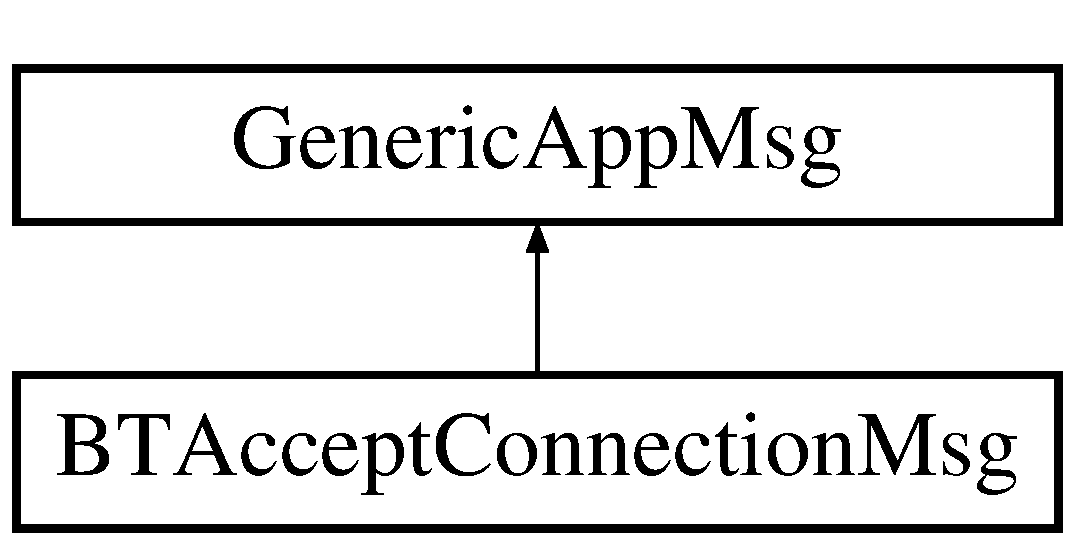
\includegraphics[height=2.000000cm]{classBTAcceptConnectionMsg}
\end{center}
\end{figure}
\subsection*{Public Member Functions}
\begin{DoxyCompactItemize}
\item 
\hyperlink{classBTAcceptConnectionMsg_add0db7db09d41c43b5ddca304d91516c}{B\+T\+Accept\+Connection\+Msg} (const char $\ast$name=N\+U\+L\+L, int kind=0)
\item 
\hyperlink{classBTAcceptConnectionMsg_ae45d54f245653f5f17b3656734a761df}{B\+T\+Accept\+Connection\+Msg} (const \hyperlink{classBTAcceptConnectionMsg}{B\+T\+Accept\+Connection\+Msg} \&other)
\item 
virtual \hyperlink{classBTAcceptConnectionMsg_a7852a9811fc9fa71ed9b77836bb5545f}{$\sim$\+B\+T\+Accept\+Connection\+Msg} ()
\item 
\hyperlink{classBTAcceptConnectionMsg}{B\+T\+Accept\+Connection\+Msg} \& \hyperlink{classBTAcceptConnectionMsg_a0c5ce6d8a8d3a4b6ddf543a400ab1ec2}{operator=} (const \hyperlink{classBTAcceptConnectionMsg}{B\+T\+Accept\+Connection\+Msg} \&other)
\item 
virtual \hyperlink{classBTAcceptConnectionMsg}{B\+T\+Accept\+Connection\+Msg} $\ast$ \hyperlink{classBTAcceptConnectionMsg_ad5edeb6c952a9ea0561113811734588a}{dup} () const 
\item 
virtual void \hyperlink{classBTAcceptConnectionMsg_a7c10fa7abe9cf9d3675f500f59cc790e}{parsim\+Pack} (c\+Comm\+Buffer $\ast$b)
\item 
virtual void \hyperlink{classBTAcceptConnectionMsg_a9aabb54dfe3eefd97bcefb28d22bc9a6}{parsim\+Unpack} (c\+Comm\+Buffer $\ast$b)
\item 
virtual bool \hyperlink{classBTAcceptConnectionMsg_a75e754e43ade635f7b220019657166e7}{accept} () const 
\item 
virtual void \hyperlink{classBTAcceptConnectionMsg_a85c7f33d626248b0395210496e5c1a93}{set\+Accept} (bool \hyperlink{classBTAcceptConnectionMsg_ab5c783dcc784f63d070c575f46426882}{accept\+\_\+var})
\end{DoxyCompactItemize}
\subsection*{Protected Member Functions}
\begin{DoxyCompactItemize}
\item 
bool \hyperlink{classBTAcceptConnectionMsg_a637bed52ab75fa20e02c7c99bb4a88af}{operator==} (const \hyperlink{classBTAcceptConnectionMsg}{B\+T\+Accept\+Connection\+Msg} \&)
\end{DoxyCompactItemize}
\subsection*{Protected Attributes}
\begin{DoxyCompactItemize}
\item 
bool \hyperlink{classBTAcceptConnectionMsg_ab5c783dcc784f63d070c575f46426882}{accept\+\_\+var}
\end{DoxyCompactItemize}


\subsection{Detailed Description}
Class generated from {\ttfamily applications/x\+Bit\+Torrent/\+B\+T\+Peer\+Wire\+Msg.\+msg} by opp\+\_\+msgc. 
\begin{DoxyPre}
message \hyperlink{classBTAcceptConnectionMsg}{BTAcceptConnectionMsg} extends GenericAppMsg
\{
    (true);\end{DoxyPre}



\begin{DoxyPre}    bool accept = true;
\}
\end{DoxyPre}
 

\subsection{Constructor \& Destructor Documentation}
\hypertarget{classBTAcceptConnectionMsg_add0db7db09d41c43b5ddca304d91516c}{}\index{B\+T\+Accept\+Connection\+Msg@{B\+T\+Accept\+Connection\+Msg}!B\+T\+Accept\+Connection\+Msg@{B\+T\+Accept\+Connection\+Msg}}
\index{B\+T\+Accept\+Connection\+Msg@{B\+T\+Accept\+Connection\+Msg}!B\+T\+Accept\+Connection\+Msg@{B\+T\+Accept\+Connection\+Msg}}
\subsubsection[{B\+T\+Accept\+Connection\+Msg(const char $\ast$name=\+N\+U\+L\+L, int kind=0)}]{\setlength{\rightskip}{0pt plus 5cm}B\+T\+Accept\+Connection\+Msg\+::\+B\+T\+Accept\+Connection\+Msg (
\begin{DoxyParamCaption}
\item[{const char $\ast$}]{name = {\ttfamily NULL}, }
\item[{int}]{kind = {\ttfamily 0}}
\end{DoxyParamCaption}
)}\label{classBTAcceptConnectionMsg_add0db7db09d41c43b5ddca304d91516c}
\hypertarget{classBTAcceptConnectionMsg_ae45d54f245653f5f17b3656734a761df}{}\index{B\+T\+Accept\+Connection\+Msg@{B\+T\+Accept\+Connection\+Msg}!B\+T\+Accept\+Connection\+Msg@{B\+T\+Accept\+Connection\+Msg}}
\index{B\+T\+Accept\+Connection\+Msg@{B\+T\+Accept\+Connection\+Msg}!B\+T\+Accept\+Connection\+Msg@{B\+T\+Accept\+Connection\+Msg}}
\subsubsection[{B\+T\+Accept\+Connection\+Msg(const B\+T\+Accept\+Connection\+Msg \&other)}]{\setlength{\rightskip}{0pt plus 5cm}B\+T\+Accept\+Connection\+Msg\+::\+B\+T\+Accept\+Connection\+Msg (
\begin{DoxyParamCaption}
\item[{const {\bf B\+T\+Accept\+Connection\+Msg} \&}]{other}
\end{DoxyParamCaption}
)}\label{classBTAcceptConnectionMsg_ae45d54f245653f5f17b3656734a761df}
\hypertarget{classBTAcceptConnectionMsg_a7852a9811fc9fa71ed9b77836bb5545f}{}\index{B\+T\+Accept\+Connection\+Msg@{B\+T\+Accept\+Connection\+Msg}!````~B\+T\+Accept\+Connection\+Msg@{$\sim$\+B\+T\+Accept\+Connection\+Msg}}
\index{````~B\+T\+Accept\+Connection\+Msg@{$\sim$\+B\+T\+Accept\+Connection\+Msg}!B\+T\+Accept\+Connection\+Msg@{B\+T\+Accept\+Connection\+Msg}}
\subsubsection[{$\sim$\+B\+T\+Accept\+Connection\+Msg()}]{\setlength{\rightskip}{0pt plus 5cm}B\+T\+Accept\+Connection\+Msg\+::$\sim$\+B\+T\+Accept\+Connection\+Msg (
\begin{DoxyParamCaption}
{}
\end{DoxyParamCaption}
)\hspace{0.3cm}{\ttfamily [virtual]}}\label{classBTAcceptConnectionMsg_a7852a9811fc9fa71ed9b77836bb5545f}


\subsection{Member Function Documentation}
\hypertarget{classBTAcceptConnectionMsg_a75e754e43ade635f7b220019657166e7}{}\index{B\+T\+Accept\+Connection\+Msg@{B\+T\+Accept\+Connection\+Msg}!accept@{accept}}
\index{accept@{accept}!B\+T\+Accept\+Connection\+Msg@{B\+T\+Accept\+Connection\+Msg}}
\subsubsection[{accept() const }]{\setlength{\rightskip}{0pt plus 5cm}bool B\+T\+Accept\+Connection\+Msg\+::accept (
\begin{DoxyParamCaption}
{}
\end{DoxyParamCaption}
) const\hspace{0.3cm}{\ttfamily [virtual]}}\label{classBTAcceptConnectionMsg_a75e754e43ade635f7b220019657166e7}
\hypertarget{classBTAcceptConnectionMsg_ad5edeb6c952a9ea0561113811734588a}{}\index{B\+T\+Accept\+Connection\+Msg@{B\+T\+Accept\+Connection\+Msg}!dup@{dup}}
\index{dup@{dup}!B\+T\+Accept\+Connection\+Msg@{B\+T\+Accept\+Connection\+Msg}}
\subsubsection[{dup() const }]{\setlength{\rightskip}{0pt plus 5cm}virtual {\bf B\+T\+Accept\+Connection\+Msg}$\ast$ B\+T\+Accept\+Connection\+Msg\+::dup (
\begin{DoxyParamCaption}
{}
\end{DoxyParamCaption}
) const\hspace{0.3cm}{\ttfamily [inline]}, {\ttfamily [virtual]}}\label{classBTAcceptConnectionMsg_ad5edeb6c952a9ea0561113811734588a}
\hypertarget{classBTAcceptConnectionMsg_a0c5ce6d8a8d3a4b6ddf543a400ab1ec2}{}\index{B\+T\+Accept\+Connection\+Msg@{B\+T\+Accept\+Connection\+Msg}!operator=@{operator=}}
\index{operator=@{operator=}!B\+T\+Accept\+Connection\+Msg@{B\+T\+Accept\+Connection\+Msg}}
\subsubsection[{operator=(const B\+T\+Accept\+Connection\+Msg \&other)}]{\setlength{\rightskip}{0pt plus 5cm}{\bf B\+T\+Accept\+Connection\+Msg} \& B\+T\+Accept\+Connection\+Msg\+::operator= (
\begin{DoxyParamCaption}
\item[{const {\bf B\+T\+Accept\+Connection\+Msg} \&}]{other}
\end{DoxyParamCaption}
)}\label{classBTAcceptConnectionMsg_a0c5ce6d8a8d3a4b6ddf543a400ab1ec2}
\hypertarget{classBTAcceptConnectionMsg_a637bed52ab75fa20e02c7c99bb4a88af}{}\index{B\+T\+Accept\+Connection\+Msg@{B\+T\+Accept\+Connection\+Msg}!operator==@{operator==}}
\index{operator==@{operator==}!B\+T\+Accept\+Connection\+Msg@{B\+T\+Accept\+Connection\+Msg}}
\subsubsection[{operator==(const B\+T\+Accept\+Connection\+Msg \&)}]{\setlength{\rightskip}{0pt plus 5cm}bool B\+T\+Accept\+Connection\+Msg\+::operator== (
\begin{DoxyParamCaption}
\item[{const {\bf B\+T\+Accept\+Connection\+Msg} \&}]{}
\end{DoxyParamCaption}
)\hspace{0.3cm}{\ttfamily [protected]}}\label{classBTAcceptConnectionMsg_a637bed52ab75fa20e02c7c99bb4a88af}
\hypertarget{classBTAcceptConnectionMsg_a7c10fa7abe9cf9d3675f500f59cc790e}{}\index{B\+T\+Accept\+Connection\+Msg@{B\+T\+Accept\+Connection\+Msg}!parsim\+Pack@{parsim\+Pack}}
\index{parsim\+Pack@{parsim\+Pack}!B\+T\+Accept\+Connection\+Msg@{B\+T\+Accept\+Connection\+Msg}}
\subsubsection[{parsim\+Pack(c\+Comm\+Buffer $\ast$b)}]{\setlength{\rightskip}{0pt plus 5cm}void B\+T\+Accept\+Connection\+Msg\+::parsim\+Pack (
\begin{DoxyParamCaption}
\item[{c\+Comm\+Buffer $\ast$}]{b}
\end{DoxyParamCaption}
)\hspace{0.3cm}{\ttfamily [virtual]}}\label{classBTAcceptConnectionMsg_a7c10fa7abe9cf9d3675f500f59cc790e}
\hypertarget{classBTAcceptConnectionMsg_a9aabb54dfe3eefd97bcefb28d22bc9a6}{}\index{B\+T\+Accept\+Connection\+Msg@{B\+T\+Accept\+Connection\+Msg}!parsim\+Unpack@{parsim\+Unpack}}
\index{parsim\+Unpack@{parsim\+Unpack}!B\+T\+Accept\+Connection\+Msg@{B\+T\+Accept\+Connection\+Msg}}
\subsubsection[{parsim\+Unpack(c\+Comm\+Buffer $\ast$b)}]{\setlength{\rightskip}{0pt plus 5cm}void B\+T\+Accept\+Connection\+Msg\+::parsim\+Unpack (
\begin{DoxyParamCaption}
\item[{c\+Comm\+Buffer $\ast$}]{b}
\end{DoxyParamCaption}
)\hspace{0.3cm}{\ttfamily [virtual]}}\label{classBTAcceptConnectionMsg_a9aabb54dfe3eefd97bcefb28d22bc9a6}
\hypertarget{classBTAcceptConnectionMsg_a85c7f33d626248b0395210496e5c1a93}{}\index{B\+T\+Accept\+Connection\+Msg@{B\+T\+Accept\+Connection\+Msg}!set\+Accept@{set\+Accept}}
\index{set\+Accept@{set\+Accept}!B\+T\+Accept\+Connection\+Msg@{B\+T\+Accept\+Connection\+Msg}}
\subsubsection[{set\+Accept(bool accept\+\_\+var)}]{\setlength{\rightskip}{0pt plus 5cm}void B\+T\+Accept\+Connection\+Msg\+::set\+Accept (
\begin{DoxyParamCaption}
\item[{bool}]{accept\+\_\+var}
\end{DoxyParamCaption}
)\hspace{0.3cm}{\ttfamily [virtual]}}\label{classBTAcceptConnectionMsg_a85c7f33d626248b0395210496e5c1a93}


\subsection{Member Data Documentation}
\hypertarget{classBTAcceptConnectionMsg_ab5c783dcc784f63d070c575f46426882}{}\index{B\+T\+Accept\+Connection\+Msg@{B\+T\+Accept\+Connection\+Msg}!accept\+\_\+var@{accept\+\_\+var}}
\index{accept\+\_\+var@{accept\+\_\+var}!B\+T\+Accept\+Connection\+Msg@{B\+T\+Accept\+Connection\+Msg}}
\subsubsection[{accept\+\_\+var}]{\setlength{\rightskip}{0pt plus 5cm}bool B\+T\+Accept\+Connection\+Msg\+::accept\+\_\+var\hspace{0.3cm}{\ttfamily [protected]}}\label{classBTAcceptConnectionMsg_ab5c783dcc784f63d070c575f46426882}


The documentation for this class was generated from the following files\+:\begin{DoxyCompactItemize}
\item 
\hyperlink{BTPeerWireMsg__m_8h}{B\+T\+Peer\+Wire\+Msg\+\_\+m.\+h}\item 
\hyperlink{BTPeerWireMsg__m_8cc}{B\+T\+Peer\+Wire\+Msg\+\_\+m.\+cc}\end{DoxyCompactItemize}

\hypertarget{classBTAcceptConnectionMsgDescriptor}{}\section{B\+T\+Accept\+Connection\+Msg\+Descriptor Class Reference}
\label{classBTAcceptConnectionMsgDescriptor}\index{B\+T\+Accept\+Connection\+Msg\+Descriptor@{B\+T\+Accept\+Connection\+Msg\+Descriptor}}
Inheritance diagram for B\+T\+Accept\+Connection\+Msg\+Descriptor\+:\begin{figure}[H]
\begin{center}
\leavevmode
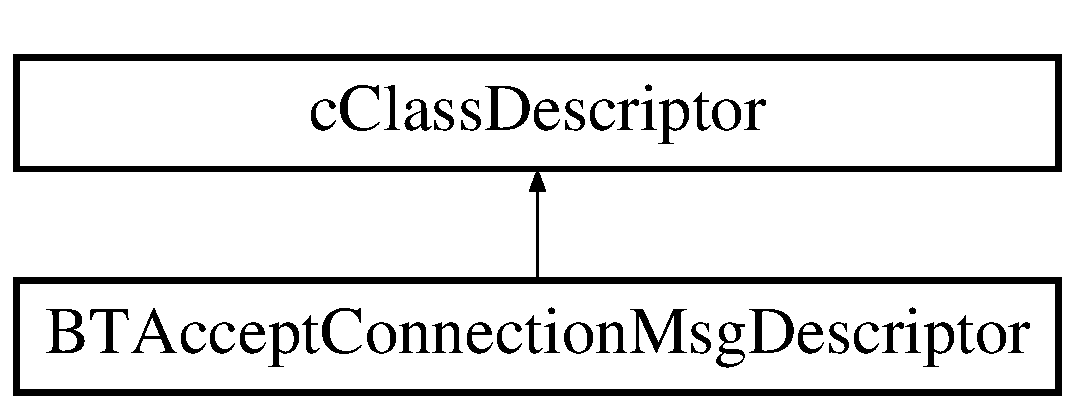
\includegraphics[height=2.000000cm]{classBTAcceptConnectionMsgDescriptor}
\end{center}
\end{figure}
\subsection*{Public Member Functions}
\begin{DoxyCompactItemize}
\item 
\hyperlink{classBTAcceptConnectionMsgDescriptor_a766c5d3f8ebf42a0cc1e4f714a0eb7bd}{B\+T\+Accept\+Connection\+Msg\+Descriptor} ()
\item 
virtual \hyperlink{classBTAcceptConnectionMsgDescriptor_ac5a7d4056ac48b6fca0b242a815a15fb}{$\sim$\+B\+T\+Accept\+Connection\+Msg\+Descriptor} ()
\item 
virtual bool \hyperlink{classBTAcceptConnectionMsgDescriptor_af2bea1ff61237e2d2ccc4bf51ed24fe8}{does\+Support} (c\+Object $\ast$obj) const 
\item 
virtual const char $\ast$ \hyperlink{classBTAcceptConnectionMsgDescriptor_ae47f50e132976322da1cd07d0ad4c3fc}{get\+Property} (const char $\ast$propertyname) const 
\item 
virtual int \hyperlink{classBTAcceptConnectionMsgDescriptor_ad65eaa39ce85d13a42ebcd154967782d}{get\+Field\+Count} (void $\ast$object) const 
\item 
virtual const char $\ast$ \hyperlink{classBTAcceptConnectionMsgDescriptor_a7cbe9fed52815e731953d278064480f4}{get\+Field\+Name} (void $\ast$object, int field) const 
\item 
virtual int \hyperlink{classBTAcceptConnectionMsgDescriptor_a944bc7e9212f7afc2f112b0d8deb60a6}{find\+Field} (void $\ast$object, const char $\ast$field\+Name) const 
\item 
virtual unsigned int \hyperlink{classBTAcceptConnectionMsgDescriptor_aa8e57d70b5626672cc9c2e18136f6ff0}{get\+Field\+Type\+Flags} (void $\ast$object, int field) const 
\item 
virtual const char $\ast$ \hyperlink{classBTAcceptConnectionMsgDescriptor_a936107d9f6e0c6c8956f24990462c5a2}{get\+Field\+Type\+String} (void $\ast$object, int field) const 
\item 
virtual const char $\ast$ \hyperlink{classBTAcceptConnectionMsgDescriptor_ac1de115d9067ad159248e4d8b1b623cd}{get\+Field\+Property} (void $\ast$object, int field, const char $\ast$propertyname) const 
\item 
virtual int \hyperlink{classBTAcceptConnectionMsgDescriptor_a56ba4d2d80ea9723cda67721b1716dc3}{get\+Array\+Size} (void $\ast$object, int field) const 
\item 
virtual std\+::string \hyperlink{classBTAcceptConnectionMsgDescriptor_af51e361233f5a13c7f4d962f11b2828b}{get\+Field\+As\+String} (void $\ast$object, int field, int i) const 
\item 
virtual bool \hyperlink{classBTAcceptConnectionMsgDescriptor_a686902fea9987f38543e8a25c71270cd}{set\+Field\+As\+String} (void $\ast$object, int field, int i, const char $\ast$value) const 
\item 
virtual const char $\ast$ \hyperlink{classBTAcceptConnectionMsgDescriptor_ae3a54f2efffc73d2387711cbeef1c80e}{get\+Field\+Struct\+Name} (void $\ast$object, int field) const 
\item 
virtual void $\ast$ \hyperlink{classBTAcceptConnectionMsgDescriptor_a4bb9d5a5a63495bce6fd6e723b15c444}{get\+Field\+Struct\+Pointer} (void $\ast$object, int field, int i) const 
\end{DoxyCompactItemize}


\subsection{Constructor \& Destructor Documentation}
\hypertarget{classBTAcceptConnectionMsgDescriptor_a766c5d3f8ebf42a0cc1e4f714a0eb7bd}{}\index{B\+T\+Accept\+Connection\+Msg\+Descriptor@{B\+T\+Accept\+Connection\+Msg\+Descriptor}!B\+T\+Accept\+Connection\+Msg\+Descriptor@{B\+T\+Accept\+Connection\+Msg\+Descriptor}}
\index{B\+T\+Accept\+Connection\+Msg\+Descriptor@{B\+T\+Accept\+Connection\+Msg\+Descriptor}!B\+T\+Accept\+Connection\+Msg\+Descriptor@{B\+T\+Accept\+Connection\+Msg\+Descriptor}}
\subsubsection[{B\+T\+Accept\+Connection\+Msg\+Descriptor()}]{\setlength{\rightskip}{0pt plus 5cm}B\+T\+Accept\+Connection\+Msg\+Descriptor\+::\+B\+T\+Accept\+Connection\+Msg\+Descriptor (
\begin{DoxyParamCaption}
{}
\end{DoxyParamCaption}
)}\label{classBTAcceptConnectionMsgDescriptor_a766c5d3f8ebf42a0cc1e4f714a0eb7bd}
\hypertarget{classBTAcceptConnectionMsgDescriptor_ac5a7d4056ac48b6fca0b242a815a15fb}{}\index{B\+T\+Accept\+Connection\+Msg\+Descriptor@{B\+T\+Accept\+Connection\+Msg\+Descriptor}!````~B\+T\+Accept\+Connection\+Msg\+Descriptor@{$\sim$\+B\+T\+Accept\+Connection\+Msg\+Descriptor}}
\index{````~B\+T\+Accept\+Connection\+Msg\+Descriptor@{$\sim$\+B\+T\+Accept\+Connection\+Msg\+Descriptor}!B\+T\+Accept\+Connection\+Msg\+Descriptor@{B\+T\+Accept\+Connection\+Msg\+Descriptor}}
\subsubsection[{$\sim$\+B\+T\+Accept\+Connection\+Msg\+Descriptor()}]{\setlength{\rightskip}{0pt plus 5cm}B\+T\+Accept\+Connection\+Msg\+Descriptor\+::$\sim$\+B\+T\+Accept\+Connection\+Msg\+Descriptor (
\begin{DoxyParamCaption}
{}
\end{DoxyParamCaption}
)\hspace{0.3cm}{\ttfamily [virtual]}}\label{classBTAcceptConnectionMsgDescriptor_ac5a7d4056ac48b6fca0b242a815a15fb}


\subsection{Member Function Documentation}
\hypertarget{classBTAcceptConnectionMsgDescriptor_af2bea1ff61237e2d2ccc4bf51ed24fe8}{}\index{B\+T\+Accept\+Connection\+Msg\+Descriptor@{B\+T\+Accept\+Connection\+Msg\+Descriptor}!does\+Support@{does\+Support}}
\index{does\+Support@{does\+Support}!B\+T\+Accept\+Connection\+Msg\+Descriptor@{B\+T\+Accept\+Connection\+Msg\+Descriptor}}
\subsubsection[{does\+Support(c\+Object $\ast$obj) const }]{\setlength{\rightskip}{0pt plus 5cm}bool B\+T\+Accept\+Connection\+Msg\+Descriptor\+::does\+Support (
\begin{DoxyParamCaption}
\item[{c\+Object $\ast$}]{obj}
\end{DoxyParamCaption}
) const\hspace{0.3cm}{\ttfamily [virtual]}}\label{classBTAcceptConnectionMsgDescriptor_af2bea1ff61237e2d2ccc4bf51ed24fe8}
\hypertarget{classBTAcceptConnectionMsgDescriptor_a944bc7e9212f7afc2f112b0d8deb60a6}{}\index{B\+T\+Accept\+Connection\+Msg\+Descriptor@{B\+T\+Accept\+Connection\+Msg\+Descriptor}!find\+Field@{find\+Field}}
\index{find\+Field@{find\+Field}!B\+T\+Accept\+Connection\+Msg\+Descriptor@{B\+T\+Accept\+Connection\+Msg\+Descriptor}}
\subsubsection[{find\+Field(void $\ast$object, const char $\ast$field\+Name) const }]{\setlength{\rightskip}{0pt plus 5cm}int B\+T\+Accept\+Connection\+Msg\+Descriptor\+::find\+Field (
\begin{DoxyParamCaption}
\item[{void $\ast$}]{object, }
\item[{const char $\ast$}]{field\+Name}
\end{DoxyParamCaption}
) const\hspace{0.3cm}{\ttfamily [virtual]}}\label{classBTAcceptConnectionMsgDescriptor_a944bc7e9212f7afc2f112b0d8deb60a6}
\hypertarget{classBTAcceptConnectionMsgDescriptor_a56ba4d2d80ea9723cda67721b1716dc3}{}\index{B\+T\+Accept\+Connection\+Msg\+Descriptor@{B\+T\+Accept\+Connection\+Msg\+Descriptor}!get\+Array\+Size@{get\+Array\+Size}}
\index{get\+Array\+Size@{get\+Array\+Size}!B\+T\+Accept\+Connection\+Msg\+Descriptor@{B\+T\+Accept\+Connection\+Msg\+Descriptor}}
\subsubsection[{get\+Array\+Size(void $\ast$object, int field) const }]{\setlength{\rightskip}{0pt plus 5cm}int B\+T\+Accept\+Connection\+Msg\+Descriptor\+::get\+Array\+Size (
\begin{DoxyParamCaption}
\item[{void $\ast$}]{object, }
\item[{int}]{field}
\end{DoxyParamCaption}
) const\hspace{0.3cm}{\ttfamily [virtual]}}\label{classBTAcceptConnectionMsgDescriptor_a56ba4d2d80ea9723cda67721b1716dc3}
\hypertarget{classBTAcceptConnectionMsgDescriptor_af51e361233f5a13c7f4d962f11b2828b}{}\index{B\+T\+Accept\+Connection\+Msg\+Descriptor@{B\+T\+Accept\+Connection\+Msg\+Descriptor}!get\+Field\+As\+String@{get\+Field\+As\+String}}
\index{get\+Field\+As\+String@{get\+Field\+As\+String}!B\+T\+Accept\+Connection\+Msg\+Descriptor@{B\+T\+Accept\+Connection\+Msg\+Descriptor}}
\subsubsection[{get\+Field\+As\+String(void $\ast$object, int field, int i) const }]{\setlength{\rightskip}{0pt plus 5cm}std\+::string B\+T\+Accept\+Connection\+Msg\+Descriptor\+::get\+Field\+As\+String (
\begin{DoxyParamCaption}
\item[{void $\ast$}]{object, }
\item[{int}]{field, }
\item[{int}]{i}
\end{DoxyParamCaption}
) const\hspace{0.3cm}{\ttfamily [virtual]}}\label{classBTAcceptConnectionMsgDescriptor_af51e361233f5a13c7f4d962f11b2828b}
\hypertarget{classBTAcceptConnectionMsgDescriptor_ad65eaa39ce85d13a42ebcd154967782d}{}\index{B\+T\+Accept\+Connection\+Msg\+Descriptor@{B\+T\+Accept\+Connection\+Msg\+Descriptor}!get\+Field\+Count@{get\+Field\+Count}}
\index{get\+Field\+Count@{get\+Field\+Count}!B\+T\+Accept\+Connection\+Msg\+Descriptor@{B\+T\+Accept\+Connection\+Msg\+Descriptor}}
\subsubsection[{get\+Field\+Count(void $\ast$object) const }]{\setlength{\rightskip}{0pt plus 5cm}int B\+T\+Accept\+Connection\+Msg\+Descriptor\+::get\+Field\+Count (
\begin{DoxyParamCaption}
\item[{void $\ast$}]{object}
\end{DoxyParamCaption}
) const\hspace{0.3cm}{\ttfamily [virtual]}}\label{classBTAcceptConnectionMsgDescriptor_ad65eaa39ce85d13a42ebcd154967782d}
\hypertarget{classBTAcceptConnectionMsgDescriptor_a7cbe9fed52815e731953d278064480f4}{}\index{B\+T\+Accept\+Connection\+Msg\+Descriptor@{B\+T\+Accept\+Connection\+Msg\+Descriptor}!get\+Field\+Name@{get\+Field\+Name}}
\index{get\+Field\+Name@{get\+Field\+Name}!B\+T\+Accept\+Connection\+Msg\+Descriptor@{B\+T\+Accept\+Connection\+Msg\+Descriptor}}
\subsubsection[{get\+Field\+Name(void $\ast$object, int field) const }]{\setlength{\rightskip}{0pt plus 5cm}const char $\ast$ B\+T\+Accept\+Connection\+Msg\+Descriptor\+::get\+Field\+Name (
\begin{DoxyParamCaption}
\item[{void $\ast$}]{object, }
\item[{int}]{field}
\end{DoxyParamCaption}
) const\hspace{0.3cm}{\ttfamily [virtual]}}\label{classBTAcceptConnectionMsgDescriptor_a7cbe9fed52815e731953d278064480f4}
\hypertarget{classBTAcceptConnectionMsgDescriptor_ac1de115d9067ad159248e4d8b1b623cd}{}\index{B\+T\+Accept\+Connection\+Msg\+Descriptor@{B\+T\+Accept\+Connection\+Msg\+Descriptor}!get\+Field\+Property@{get\+Field\+Property}}
\index{get\+Field\+Property@{get\+Field\+Property}!B\+T\+Accept\+Connection\+Msg\+Descriptor@{B\+T\+Accept\+Connection\+Msg\+Descriptor}}
\subsubsection[{get\+Field\+Property(void $\ast$object, int field, const char $\ast$propertyname) const }]{\setlength{\rightskip}{0pt plus 5cm}const char $\ast$ B\+T\+Accept\+Connection\+Msg\+Descriptor\+::get\+Field\+Property (
\begin{DoxyParamCaption}
\item[{void $\ast$}]{object, }
\item[{int}]{field, }
\item[{const char $\ast$}]{propertyname}
\end{DoxyParamCaption}
) const\hspace{0.3cm}{\ttfamily [virtual]}}\label{classBTAcceptConnectionMsgDescriptor_ac1de115d9067ad159248e4d8b1b623cd}
\hypertarget{classBTAcceptConnectionMsgDescriptor_ae3a54f2efffc73d2387711cbeef1c80e}{}\index{B\+T\+Accept\+Connection\+Msg\+Descriptor@{B\+T\+Accept\+Connection\+Msg\+Descriptor}!get\+Field\+Struct\+Name@{get\+Field\+Struct\+Name}}
\index{get\+Field\+Struct\+Name@{get\+Field\+Struct\+Name}!B\+T\+Accept\+Connection\+Msg\+Descriptor@{B\+T\+Accept\+Connection\+Msg\+Descriptor}}
\subsubsection[{get\+Field\+Struct\+Name(void $\ast$object, int field) const }]{\setlength{\rightskip}{0pt plus 5cm}const char $\ast$ B\+T\+Accept\+Connection\+Msg\+Descriptor\+::get\+Field\+Struct\+Name (
\begin{DoxyParamCaption}
\item[{void $\ast$}]{object, }
\item[{int}]{field}
\end{DoxyParamCaption}
) const\hspace{0.3cm}{\ttfamily [virtual]}}\label{classBTAcceptConnectionMsgDescriptor_ae3a54f2efffc73d2387711cbeef1c80e}
\hypertarget{classBTAcceptConnectionMsgDescriptor_a4bb9d5a5a63495bce6fd6e723b15c444}{}\index{B\+T\+Accept\+Connection\+Msg\+Descriptor@{B\+T\+Accept\+Connection\+Msg\+Descriptor}!get\+Field\+Struct\+Pointer@{get\+Field\+Struct\+Pointer}}
\index{get\+Field\+Struct\+Pointer@{get\+Field\+Struct\+Pointer}!B\+T\+Accept\+Connection\+Msg\+Descriptor@{B\+T\+Accept\+Connection\+Msg\+Descriptor}}
\subsubsection[{get\+Field\+Struct\+Pointer(void $\ast$object, int field, int i) const }]{\setlength{\rightskip}{0pt plus 5cm}void $\ast$ B\+T\+Accept\+Connection\+Msg\+Descriptor\+::get\+Field\+Struct\+Pointer (
\begin{DoxyParamCaption}
\item[{void $\ast$}]{object, }
\item[{int}]{field, }
\item[{int}]{i}
\end{DoxyParamCaption}
) const\hspace{0.3cm}{\ttfamily [virtual]}}\label{classBTAcceptConnectionMsgDescriptor_a4bb9d5a5a63495bce6fd6e723b15c444}
\hypertarget{classBTAcceptConnectionMsgDescriptor_aa8e57d70b5626672cc9c2e18136f6ff0}{}\index{B\+T\+Accept\+Connection\+Msg\+Descriptor@{B\+T\+Accept\+Connection\+Msg\+Descriptor}!get\+Field\+Type\+Flags@{get\+Field\+Type\+Flags}}
\index{get\+Field\+Type\+Flags@{get\+Field\+Type\+Flags}!B\+T\+Accept\+Connection\+Msg\+Descriptor@{B\+T\+Accept\+Connection\+Msg\+Descriptor}}
\subsubsection[{get\+Field\+Type\+Flags(void $\ast$object, int field) const }]{\setlength{\rightskip}{0pt plus 5cm}unsigned int B\+T\+Accept\+Connection\+Msg\+Descriptor\+::get\+Field\+Type\+Flags (
\begin{DoxyParamCaption}
\item[{void $\ast$}]{object, }
\item[{int}]{field}
\end{DoxyParamCaption}
) const\hspace{0.3cm}{\ttfamily [virtual]}}\label{classBTAcceptConnectionMsgDescriptor_aa8e57d70b5626672cc9c2e18136f6ff0}
\hypertarget{classBTAcceptConnectionMsgDescriptor_a936107d9f6e0c6c8956f24990462c5a2}{}\index{B\+T\+Accept\+Connection\+Msg\+Descriptor@{B\+T\+Accept\+Connection\+Msg\+Descriptor}!get\+Field\+Type\+String@{get\+Field\+Type\+String}}
\index{get\+Field\+Type\+String@{get\+Field\+Type\+String}!B\+T\+Accept\+Connection\+Msg\+Descriptor@{B\+T\+Accept\+Connection\+Msg\+Descriptor}}
\subsubsection[{get\+Field\+Type\+String(void $\ast$object, int field) const }]{\setlength{\rightskip}{0pt plus 5cm}const char $\ast$ B\+T\+Accept\+Connection\+Msg\+Descriptor\+::get\+Field\+Type\+String (
\begin{DoxyParamCaption}
\item[{void $\ast$}]{object, }
\item[{int}]{field}
\end{DoxyParamCaption}
) const\hspace{0.3cm}{\ttfamily [virtual]}}\label{classBTAcceptConnectionMsgDescriptor_a936107d9f6e0c6c8956f24990462c5a2}
\hypertarget{classBTAcceptConnectionMsgDescriptor_ae47f50e132976322da1cd07d0ad4c3fc}{}\index{B\+T\+Accept\+Connection\+Msg\+Descriptor@{B\+T\+Accept\+Connection\+Msg\+Descriptor}!get\+Property@{get\+Property}}
\index{get\+Property@{get\+Property}!B\+T\+Accept\+Connection\+Msg\+Descriptor@{B\+T\+Accept\+Connection\+Msg\+Descriptor}}
\subsubsection[{get\+Property(const char $\ast$propertyname) const }]{\setlength{\rightskip}{0pt plus 5cm}const char $\ast$ B\+T\+Accept\+Connection\+Msg\+Descriptor\+::get\+Property (
\begin{DoxyParamCaption}
\item[{const char $\ast$}]{propertyname}
\end{DoxyParamCaption}
) const\hspace{0.3cm}{\ttfamily [virtual]}}\label{classBTAcceptConnectionMsgDescriptor_ae47f50e132976322da1cd07d0ad4c3fc}
\hypertarget{classBTAcceptConnectionMsgDescriptor_a686902fea9987f38543e8a25c71270cd}{}\index{B\+T\+Accept\+Connection\+Msg\+Descriptor@{B\+T\+Accept\+Connection\+Msg\+Descriptor}!set\+Field\+As\+String@{set\+Field\+As\+String}}
\index{set\+Field\+As\+String@{set\+Field\+As\+String}!B\+T\+Accept\+Connection\+Msg\+Descriptor@{B\+T\+Accept\+Connection\+Msg\+Descriptor}}
\subsubsection[{set\+Field\+As\+String(void $\ast$object, int field, int i, const char $\ast$value) const }]{\setlength{\rightskip}{0pt plus 5cm}bool B\+T\+Accept\+Connection\+Msg\+Descriptor\+::set\+Field\+As\+String (
\begin{DoxyParamCaption}
\item[{void $\ast$}]{object, }
\item[{int}]{field, }
\item[{int}]{i, }
\item[{const char $\ast$}]{value}
\end{DoxyParamCaption}
) const\hspace{0.3cm}{\ttfamily [virtual]}}\label{classBTAcceptConnectionMsgDescriptor_a686902fea9987f38543e8a25c71270cd}


The documentation for this class was generated from the following file\+:\begin{DoxyCompactItemize}
\item 
\hyperlink{BTPeerWireMsg__m_8cc}{B\+T\+Peer\+Wire\+Msg\+\_\+m.\+cc}\end{DoxyCompactItemize}

\hypertarget{classBTBitfieldMsg}{}\section{B\+T\+Bitfield\+Msg Class Reference}
\label{classBTBitfieldMsg}\index{B\+T\+Bitfield\+Msg@{B\+T\+Bitfield\+Msg}}


{\ttfamily \#include $<$B\+T\+Peer\+Wire\+Msg\+\_\+m.\+h$>$}

Inheritance diagram for B\+T\+Bitfield\+Msg\+:\begin{figure}[H]
\begin{center}
\leavevmode
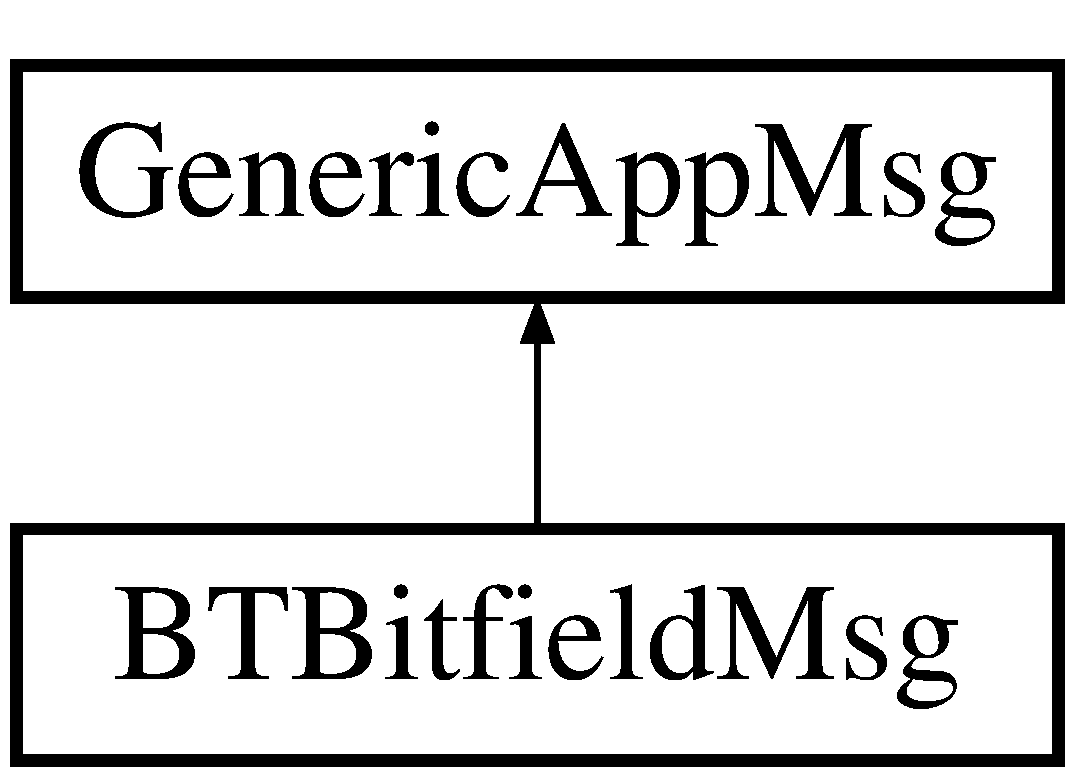
\includegraphics[height=2.000000cm]{classBTBitfieldMsg}
\end{center}
\end{figure}
\subsection*{Public Member Functions}
\begin{DoxyCompactItemize}
\item 
\hyperlink{classBTBitfieldMsg_ae71b7868e1f9b27629f6f391b352c911}{B\+T\+Bitfield\+Msg} (const char $\ast$name=N\+U\+L\+L, int kind=0)
\item 
\hyperlink{classBTBitfieldMsg_a3106cbcfeff6258360d37dd64ac337f8}{B\+T\+Bitfield\+Msg} (const \hyperlink{classBTBitfieldMsg}{B\+T\+Bitfield\+Msg} \&other)
\item 
virtual \hyperlink{classBTBitfieldMsg_a9233620b684aec4bbb3c1ae5db992962}{$\sim$\+B\+T\+Bitfield\+Msg} ()
\item 
\hyperlink{classBTBitfieldMsg}{B\+T\+Bitfield\+Msg} \& \hyperlink{classBTBitfieldMsg_a08e92e1add02c4b44de4b3c9805dff07}{operator=} (const \hyperlink{classBTBitfieldMsg}{B\+T\+Bitfield\+Msg} \&other)
\item 
virtual \hyperlink{classBTBitfieldMsg}{B\+T\+Bitfield\+Msg} $\ast$ \hyperlink{classBTBitfieldMsg_aa868c1c4c6f41c1e39eb740e7cd3f55f}{dup} () const 
\item 
virtual void \hyperlink{classBTBitfieldMsg_a8ae00cea21bf256b774a6a618516a1df}{parsim\+Pack} (c\+Comm\+Buffer $\ast$b)
\item 
virtual void \hyperlink{classBTBitfieldMsg_a793a3596151d3d008bf8268b30ab30a1}{parsim\+Unpack} (c\+Comm\+Buffer $\ast$b)
\item 
virtual int \hyperlink{classBTBitfieldMsg_a4b19acf793716974286b30e51a4ae6a6}{length\+\_\+prefix} () const 
\item 
virtual void \hyperlink{classBTBitfieldMsg_aa8a72966bdfa717d283efd63d1c77bc8}{set\+Length\+\_\+prefix} (int \hyperlink{classBTBitfieldMsg_a9040140b874e54a8dc67450a91ffb71b}{length\+\_\+prefix\+\_\+var})
\item 
virtual unsigned short \hyperlink{classBTBitfieldMsg_a0ab3c6abff00a0efe57031e83b34a926}{I\+D} () const 
\item 
virtual void \hyperlink{classBTBitfieldMsg_a80d7334c46ea207cdd2c269c155b7332}{set\+I\+D} (unsigned short \hyperlink{classBTBitfieldMsg_a9b73c5b2ce95effc48060f120ac49062}{I\+D\+\_\+var})
\item 
virtual void \hyperlink{classBTBitfieldMsg_a502a312ee81437e26312b20d3889d548}{set\+Bitfield\+Array\+Size} (unsigned int size)
\item 
virtual unsigned int \hyperlink{classBTBitfieldMsg_adac91263151d7859e2f0465172fa01d4}{bitfield\+Array\+Size} () const 
\item 
virtual bool \hyperlink{classBTBitfieldMsg_acc2ab9019bbbbdf32111a21240cc23d9}{bitfield} (unsigned int k) const 
\item 
virtual void \hyperlink{classBTBitfieldMsg_a5e0e12234ad65a8e1b386229951b7b74}{set\+Bitfield} (unsigned int k, bool \hyperlink{classBTBitfieldMsg_aef51fc463d47fdaefb5db5eec449448d}{bitfield\+\_\+var})
\end{DoxyCompactItemize}
\subsection*{Protected Member Functions}
\begin{DoxyCompactItemize}
\item 
bool \hyperlink{classBTBitfieldMsg_ad6f057b2001791771943f62c5c796a9c}{operator==} (const \hyperlink{classBTBitfieldMsg}{B\+T\+Bitfield\+Msg} \&)
\end{DoxyCompactItemize}
\subsection*{Protected Attributes}
\begin{DoxyCompactItemize}
\item 
int \hyperlink{classBTBitfieldMsg_a9040140b874e54a8dc67450a91ffb71b}{length\+\_\+prefix\+\_\+var}
\item 
unsigned short \hyperlink{classBTBitfieldMsg_a9b73c5b2ce95effc48060f120ac49062}{I\+D\+\_\+var}
\item 
bool $\ast$ \hyperlink{classBTBitfieldMsg_aef51fc463d47fdaefb5db5eec449448d}{bitfield\+\_\+var}
\item 
unsigned int \hyperlink{classBTBitfieldMsg_aed336aa06c9d5bf68f7d16e552c79ef3}{bitfield\+\_\+arraysize}
\end{DoxyCompactItemize}


\subsection{Constructor \& Destructor Documentation}
\hypertarget{classBTBitfieldMsg_ae71b7868e1f9b27629f6f391b352c911}{}\index{B\+T\+Bitfield\+Msg@{B\+T\+Bitfield\+Msg}!B\+T\+Bitfield\+Msg@{B\+T\+Bitfield\+Msg}}
\index{B\+T\+Bitfield\+Msg@{B\+T\+Bitfield\+Msg}!B\+T\+Bitfield\+Msg@{B\+T\+Bitfield\+Msg}}
\subsubsection[{B\+T\+Bitfield\+Msg(const char $\ast$name=\+N\+U\+L\+L, int kind=0)}]{\setlength{\rightskip}{0pt plus 5cm}B\+T\+Bitfield\+Msg\+::\+B\+T\+Bitfield\+Msg (
\begin{DoxyParamCaption}
\item[{const char $\ast$}]{name = {\ttfamily NULL}, }
\item[{int}]{kind = {\ttfamily 0}}
\end{DoxyParamCaption}
)}\label{classBTBitfieldMsg_ae71b7868e1f9b27629f6f391b352c911}
\hypertarget{classBTBitfieldMsg_a3106cbcfeff6258360d37dd64ac337f8}{}\index{B\+T\+Bitfield\+Msg@{B\+T\+Bitfield\+Msg}!B\+T\+Bitfield\+Msg@{B\+T\+Bitfield\+Msg}}
\index{B\+T\+Bitfield\+Msg@{B\+T\+Bitfield\+Msg}!B\+T\+Bitfield\+Msg@{B\+T\+Bitfield\+Msg}}
\subsubsection[{B\+T\+Bitfield\+Msg(const B\+T\+Bitfield\+Msg \&other)}]{\setlength{\rightskip}{0pt plus 5cm}B\+T\+Bitfield\+Msg\+::\+B\+T\+Bitfield\+Msg (
\begin{DoxyParamCaption}
\item[{const {\bf B\+T\+Bitfield\+Msg} \&}]{other}
\end{DoxyParamCaption}
)}\label{classBTBitfieldMsg_a3106cbcfeff6258360d37dd64ac337f8}
\hypertarget{classBTBitfieldMsg_a9233620b684aec4bbb3c1ae5db992962}{}\index{B\+T\+Bitfield\+Msg@{B\+T\+Bitfield\+Msg}!````~B\+T\+Bitfield\+Msg@{$\sim$\+B\+T\+Bitfield\+Msg}}
\index{````~B\+T\+Bitfield\+Msg@{$\sim$\+B\+T\+Bitfield\+Msg}!B\+T\+Bitfield\+Msg@{B\+T\+Bitfield\+Msg}}
\subsubsection[{$\sim$\+B\+T\+Bitfield\+Msg()}]{\setlength{\rightskip}{0pt plus 5cm}B\+T\+Bitfield\+Msg\+::$\sim$\+B\+T\+Bitfield\+Msg (
\begin{DoxyParamCaption}
{}
\end{DoxyParamCaption}
)\hspace{0.3cm}{\ttfamily [virtual]}}\label{classBTBitfieldMsg_a9233620b684aec4bbb3c1ae5db992962}


\subsection{Member Function Documentation}
\hypertarget{classBTBitfieldMsg_acc2ab9019bbbbdf32111a21240cc23d9}{}\index{B\+T\+Bitfield\+Msg@{B\+T\+Bitfield\+Msg}!bitfield@{bitfield}}
\index{bitfield@{bitfield}!B\+T\+Bitfield\+Msg@{B\+T\+Bitfield\+Msg}}
\subsubsection[{bitfield(unsigned int k) const }]{\setlength{\rightskip}{0pt plus 5cm}bool B\+T\+Bitfield\+Msg\+::bitfield (
\begin{DoxyParamCaption}
\item[{unsigned int}]{k}
\end{DoxyParamCaption}
) const\hspace{0.3cm}{\ttfamily [virtual]}}\label{classBTBitfieldMsg_acc2ab9019bbbbdf32111a21240cc23d9}
\hypertarget{classBTBitfieldMsg_adac91263151d7859e2f0465172fa01d4}{}\index{B\+T\+Bitfield\+Msg@{B\+T\+Bitfield\+Msg}!bitfield\+Array\+Size@{bitfield\+Array\+Size}}
\index{bitfield\+Array\+Size@{bitfield\+Array\+Size}!B\+T\+Bitfield\+Msg@{B\+T\+Bitfield\+Msg}}
\subsubsection[{bitfield\+Array\+Size() const }]{\setlength{\rightskip}{0pt plus 5cm}unsigned int B\+T\+Bitfield\+Msg\+::bitfield\+Array\+Size (
\begin{DoxyParamCaption}
{}
\end{DoxyParamCaption}
) const\hspace{0.3cm}{\ttfamily [virtual]}}\label{classBTBitfieldMsg_adac91263151d7859e2f0465172fa01d4}
\hypertarget{classBTBitfieldMsg_aa868c1c4c6f41c1e39eb740e7cd3f55f}{}\index{B\+T\+Bitfield\+Msg@{B\+T\+Bitfield\+Msg}!dup@{dup}}
\index{dup@{dup}!B\+T\+Bitfield\+Msg@{B\+T\+Bitfield\+Msg}}
\subsubsection[{dup() const }]{\setlength{\rightskip}{0pt plus 5cm}virtual {\bf B\+T\+Bitfield\+Msg}$\ast$ B\+T\+Bitfield\+Msg\+::dup (
\begin{DoxyParamCaption}
{}
\end{DoxyParamCaption}
) const\hspace{0.3cm}{\ttfamily [inline]}, {\ttfamily [virtual]}}\label{classBTBitfieldMsg_aa868c1c4c6f41c1e39eb740e7cd3f55f}
\hypertarget{classBTBitfieldMsg_a0ab3c6abff00a0efe57031e83b34a926}{}\index{B\+T\+Bitfield\+Msg@{B\+T\+Bitfield\+Msg}!I\+D@{I\+D}}
\index{I\+D@{I\+D}!B\+T\+Bitfield\+Msg@{B\+T\+Bitfield\+Msg}}
\subsubsection[{I\+D() const }]{\setlength{\rightskip}{0pt plus 5cm}unsigned short B\+T\+Bitfield\+Msg\+::\+I\+D (
\begin{DoxyParamCaption}
{}
\end{DoxyParamCaption}
) const\hspace{0.3cm}{\ttfamily [virtual]}}\label{classBTBitfieldMsg_a0ab3c6abff00a0efe57031e83b34a926}
\hypertarget{classBTBitfieldMsg_a4b19acf793716974286b30e51a4ae6a6}{}\index{B\+T\+Bitfield\+Msg@{B\+T\+Bitfield\+Msg}!length\+\_\+prefix@{length\+\_\+prefix}}
\index{length\+\_\+prefix@{length\+\_\+prefix}!B\+T\+Bitfield\+Msg@{B\+T\+Bitfield\+Msg}}
\subsubsection[{length\+\_\+prefix() const }]{\setlength{\rightskip}{0pt plus 5cm}int B\+T\+Bitfield\+Msg\+::length\+\_\+prefix (
\begin{DoxyParamCaption}
{}
\end{DoxyParamCaption}
) const\hspace{0.3cm}{\ttfamily [virtual]}}\label{classBTBitfieldMsg_a4b19acf793716974286b30e51a4ae6a6}
\hypertarget{classBTBitfieldMsg_a08e92e1add02c4b44de4b3c9805dff07}{}\index{B\+T\+Bitfield\+Msg@{B\+T\+Bitfield\+Msg}!operator=@{operator=}}
\index{operator=@{operator=}!B\+T\+Bitfield\+Msg@{B\+T\+Bitfield\+Msg}}
\subsubsection[{operator=(const B\+T\+Bitfield\+Msg \&other)}]{\setlength{\rightskip}{0pt plus 5cm}{\bf B\+T\+Bitfield\+Msg} \& B\+T\+Bitfield\+Msg\+::operator= (
\begin{DoxyParamCaption}
\item[{const {\bf B\+T\+Bitfield\+Msg} \&}]{other}
\end{DoxyParamCaption}
)}\label{classBTBitfieldMsg_a08e92e1add02c4b44de4b3c9805dff07}
\hypertarget{classBTBitfieldMsg_ad6f057b2001791771943f62c5c796a9c}{}\index{B\+T\+Bitfield\+Msg@{B\+T\+Bitfield\+Msg}!operator==@{operator==}}
\index{operator==@{operator==}!B\+T\+Bitfield\+Msg@{B\+T\+Bitfield\+Msg}}
\subsubsection[{operator==(const B\+T\+Bitfield\+Msg \&)}]{\setlength{\rightskip}{0pt plus 5cm}bool B\+T\+Bitfield\+Msg\+::operator== (
\begin{DoxyParamCaption}
\item[{const {\bf B\+T\+Bitfield\+Msg} \&}]{}
\end{DoxyParamCaption}
)\hspace{0.3cm}{\ttfamily [protected]}}\label{classBTBitfieldMsg_ad6f057b2001791771943f62c5c796a9c}
\hypertarget{classBTBitfieldMsg_a8ae00cea21bf256b774a6a618516a1df}{}\index{B\+T\+Bitfield\+Msg@{B\+T\+Bitfield\+Msg}!parsim\+Pack@{parsim\+Pack}}
\index{parsim\+Pack@{parsim\+Pack}!B\+T\+Bitfield\+Msg@{B\+T\+Bitfield\+Msg}}
\subsubsection[{parsim\+Pack(c\+Comm\+Buffer $\ast$b)}]{\setlength{\rightskip}{0pt plus 5cm}void B\+T\+Bitfield\+Msg\+::parsim\+Pack (
\begin{DoxyParamCaption}
\item[{c\+Comm\+Buffer $\ast$}]{b}
\end{DoxyParamCaption}
)\hspace{0.3cm}{\ttfamily [virtual]}}\label{classBTBitfieldMsg_a8ae00cea21bf256b774a6a618516a1df}
\hypertarget{classBTBitfieldMsg_a793a3596151d3d008bf8268b30ab30a1}{}\index{B\+T\+Bitfield\+Msg@{B\+T\+Bitfield\+Msg}!parsim\+Unpack@{parsim\+Unpack}}
\index{parsim\+Unpack@{parsim\+Unpack}!B\+T\+Bitfield\+Msg@{B\+T\+Bitfield\+Msg}}
\subsubsection[{parsim\+Unpack(c\+Comm\+Buffer $\ast$b)}]{\setlength{\rightskip}{0pt plus 5cm}void B\+T\+Bitfield\+Msg\+::parsim\+Unpack (
\begin{DoxyParamCaption}
\item[{c\+Comm\+Buffer $\ast$}]{b}
\end{DoxyParamCaption}
)\hspace{0.3cm}{\ttfamily [virtual]}}\label{classBTBitfieldMsg_a793a3596151d3d008bf8268b30ab30a1}
\hypertarget{classBTBitfieldMsg_a5e0e12234ad65a8e1b386229951b7b74}{}\index{B\+T\+Bitfield\+Msg@{B\+T\+Bitfield\+Msg}!set\+Bitfield@{set\+Bitfield}}
\index{set\+Bitfield@{set\+Bitfield}!B\+T\+Bitfield\+Msg@{B\+T\+Bitfield\+Msg}}
\subsubsection[{set\+Bitfield(unsigned int k, bool bitfield\+\_\+var)}]{\setlength{\rightskip}{0pt plus 5cm}void B\+T\+Bitfield\+Msg\+::set\+Bitfield (
\begin{DoxyParamCaption}
\item[{unsigned int}]{k, }
\item[{bool}]{bitfield\+\_\+var}
\end{DoxyParamCaption}
)\hspace{0.3cm}{\ttfamily [virtual]}}\label{classBTBitfieldMsg_a5e0e12234ad65a8e1b386229951b7b74}
\hypertarget{classBTBitfieldMsg_a502a312ee81437e26312b20d3889d548}{}\index{B\+T\+Bitfield\+Msg@{B\+T\+Bitfield\+Msg}!set\+Bitfield\+Array\+Size@{set\+Bitfield\+Array\+Size}}
\index{set\+Bitfield\+Array\+Size@{set\+Bitfield\+Array\+Size}!B\+T\+Bitfield\+Msg@{B\+T\+Bitfield\+Msg}}
\subsubsection[{set\+Bitfield\+Array\+Size(unsigned int size)}]{\setlength{\rightskip}{0pt plus 5cm}void B\+T\+Bitfield\+Msg\+::set\+Bitfield\+Array\+Size (
\begin{DoxyParamCaption}
\item[{unsigned int}]{size}
\end{DoxyParamCaption}
)\hspace{0.3cm}{\ttfamily [virtual]}}\label{classBTBitfieldMsg_a502a312ee81437e26312b20d3889d548}
\hypertarget{classBTBitfieldMsg_a80d7334c46ea207cdd2c269c155b7332}{}\index{B\+T\+Bitfield\+Msg@{B\+T\+Bitfield\+Msg}!set\+I\+D@{set\+I\+D}}
\index{set\+I\+D@{set\+I\+D}!B\+T\+Bitfield\+Msg@{B\+T\+Bitfield\+Msg}}
\subsubsection[{set\+I\+D(unsigned short I\+D\+\_\+var)}]{\setlength{\rightskip}{0pt plus 5cm}void B\+T\+Bitfield\+Msg\+::set\+I\+D (
\begin{DoxyParamCaption}
\item[{unsigned short}]{I\+D\+\_\+var}
\end{DoxyParamCaption}
)\hspace{0.3cm}{\ttfamily [virtual]}}\label{classBTBitfieldMsg_a80d7334c46ea207cdd2c269c155b7332}
\hypertarget{classBTBitfieldMsg_aa8a72966bdfa717d283efd63d1c77bc8}{}\index{B\+T\+Bitfield\+Msg@{B\+T\+Bitfield\+Msg}!set\+Length\+\_\+prefix@{set\+Length\+\_\+prefix}}
\index{set\+Length\+\_\+prefix@{set\+Length\+\_\+prefix}!B\+T\+Bitfield\+Msg@{B\+T\+Bitfield\+Msg}}
\subsubsection[{set\+Length\+\_\+prefix(int length\+\_\+prefix\+\_\+var)}]{\setlength{\rightskip}{0pt plus 5cm}void B\+T\+Bitfield\+Msg\+::set\+Length\+\_\+prefix (
\begin{DoxyParamCaption}
\item[{int}]{length\+\_\+prefix\+\_\+var}
\end{DoxyParamCaption}
)\hspace{0.3cm}{\ttfamily [virtual]}}\label{classBTBitfieldMsg_aa8a72966bdfa717d283efd63d1c77bc8}


\subsection{Member Data Documentation}
\hypertarget{classBTBitfieldMsg_aed336aa06c9d5bf68f7d16e552c79ef3}{}\index{B\+T\+Bitfield\+Msg@{B\+T\+Bitfield\+Msg}!bitfield\+\_\+arraysize@{bitfield\+\_\+arraysize}}
\index{bitfield\+\_\+arraysize@{bitfield\+\_\+arraysize}!B\+T\+Bitfield\+Msg@{B\+T\+Bitfield\+Msg}}
\subsubsection[{bitfield\+\_\+arraysize}]{\setlength{\rightskip}{0pt plus 5cm}unsigned int B\+T\+Bitfield\+Msg\+::bitfield\+\_\+arraysize\hspace{0.3cm}{\ttfamily [protected]}}\label{classBTBitfieldMsg_aed336aa06c9d5bf68f7d16e552c79ef3}
\hypertarget{classBTBitfieldMsg_aef51fc463d47fdaefb5db5eec449448d}{}\index{B\+T\+Bitfield\+Msg@{B\+T\+Bitfield\+Msg}!bitfield\+\_\+var@{bitfield\+\_\+var}}
\index{bitfield\+\_\+var@{bitfield\+\_\+var}!B\+T\+Bitfield\+Msg@{B\+T\+Bitfield\+Msg}}
\subsubsection[{bitfield\+\_\+var}]{\setlength{\rightskip}{0pt plus 5cm}bool$\ast$ B\+T\+Bitfield\+Msg\+::bitfield\+\_\+var\hspace{0.3cm}{\ttfamily [protected]}}\label{classBTBitfieldMsg_aef51fc463d47fdaefb5db5eec449448d}
\hypertarget{classBTBitfieldMsg_a9b73c5b2ce95effc48060f120ac49062}{}\index{B\+T\+Bitfield\+Msg@{B\+T\+Bitfield\+Msg}!I\+D\+\_\+var@{I\+D\+\_\+var}}
\index{I\+D\+\_\+var@{I\+D\+\_\+var}!B\+T\+Bitfield\+Msg@{B\+T\+Bitfield\+Msg}}
\subsubsection[{I\+D\+\_\+var}]{\setlength{\rightskip}{0pt plus 5cm}unsigned short B\+T\+Bitfield\+Msg\+::\+I\+D\+\_\+var\hspace{0.3cm}{\ttfamily [protected]}}\label{classBTBitfieldMsg_a9b73c5b2ce95effc48060f120ac49062}
\hypertarget{classBTBitfieldMsg_a9040140b874e54a8dc67450a91ffb71b}{}\index{B\+T\+Bitfield\+Msg@{B\+T\+Bitfield\+Msg}!length\+\_\+prefix\+\_\+var@{length\+\_\+prefix\+\_\+var}}
\index{length\+\_\+prefix\+\_\+var@{length\+\_\+prefix\+\_\+var}!B\+T\+Bitfield\+Msg@{B\+T\+Bitfield\+Msg}}
\subsubsection[{length\+\_\+prefix\+\_\+var}]{\setlength{\rightskip}{0pt plus 5cm}int B\+T\+Bitfield\+Msg\+::length\+\_\+prefix\+\_\+var\hspace{0.3cm}{\ttfamily [protected]}}\label{classBTBitfieldMsg_a9040140b874e54a8dc67450a91ffb71b}


The documentation for this class was generated from the following files\+:\begin{DoxyCompactItemize}
\item 
\hyperlink{BTPeerWireMsg__m_8h}{B\+T\+Peer\+Wire\+Msg\+\_\+m.\+h}\item 
\hyperlink{BTPeerWireMsg__m_8cc}{B\+T\+Peer\+Wire\+Msg\+\_\+m.\+cc}\end{DoxyCompactItemize}

\hypertarget{classBTBitfieldMsgDescriptor}{}\section{B\+T\+Bitfield\+Msg\+Descriptor Class Reference}
\label{classBTBitfieldMsgDescriptor}\index{B\+T\+Bitfield\+Msg\+Descriptor@{B\+T\+Bitfield\+Msg\+Descriptor}}
Inheritance diagram for B\+T\+Bitfield\+Msg\+Descriptor\+:\begin{figure}[H]
\begin{center}
\leavevmode
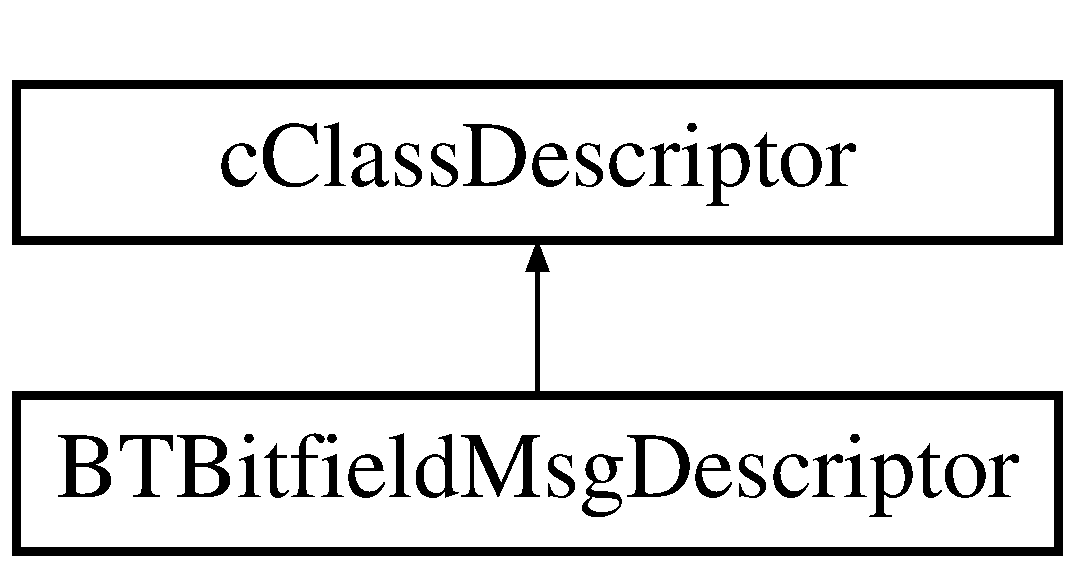
\includegraphics[height=2.000000cm]{classBTBitfieldMsgDescriptor}
\end{center}
\end{figure}
\subsection*{Public Member Functions}
\begin{DoxyCompactItemize}
\item 
\hyperlink{classBTBitfieldMsgDescriptor_ad4051badc3177f22c72bfd32065872f3}{B\+T\+Bitfield\+Msg\+Descriptor} ()
\item 
virtual \hyperlink{classBTBitfieldMsgDescriptor_acf7e4166af1697dd00657f7980d71756}{$\sim$\+B\+T\+Bitfield\+Msg\+Descriptor} ()
\item 
virtual bool \hyperlink{classBTBitfieldMsgDescriptor_a8435f3275120e0e76f31a21061b6f4d8}{does\+Support} (c\+Object $\ast$obj) const 
\item 
virtual const char $\ast$ \hyperlink{classBTBitfieldMsgDescriptor_a5b215b7ab75a11e0fb21f517b14937ad}{get\+Property} (const char $\ast$propertyname) const 
\item 
virtual int \hyperlink{classBTBitfieldMsgDescriptor_a60200f125a6d0704b580b25b0e21e2f8}{get\+Field\+Count} (void $\ast$object) const 
\item 
virtual const char $\ast$ \hyperlink{classBTBitfieldMsgDescriptor_a780143d4b4bcc4b5132a02d83fb77207}{get\+Field\+Name} (void $\ast$object, int field) const 
\item 
virtual int \hyperlink{classBTBitfieldMsgDescriptor_a3299272ebd49d6e2a8bedbf033111c53}{find\+Field} (void $\ast$object, const char $\ast$field\+Name) const 
\item 
virtual unsigned int \hyperlink{classBTBitfieldMsgDescriptor_a27e94d0cf2686869684b47a718da76c7}{get\+Field\+Type\+Flags} (void $\ast$object, int field) const 
\item 
virtual const char $\ast$ \hyperlink{classBTBitfieldMsgDescriptor_a5868329af54dad534959851554201185}{get\+Field\+Type\+String} (void $\ast$object, int field) const 
\item 
virtual const char $\ast$ \hyperlink{classBTBitfieldMsgDescriptor_a4dc4158c7651028bd995cce6cf5bfe23}{get\+Field\+Property} (void $\ast$object, int field, const char $\ast$propertyname) const 
\item 
virtual int \hyperlink{classBTBitfieldMsgDescriptor_aa0599043f7af977294a91d14c1807d29}{get\+Array\+Size} (void $\ast$object, int field) const 
\item 
virtual std\+::string \hyperlink{classBTBitfieldMsgDescriptor_ad9261d5de7428a2d5122259aa6519782}{get\+Field\+As\+String} (void $\ast$object, int field, int i) const 
\item 
virtual bool \hyperlink{classBTBitfieldMsgDescriptor_a2c1652639718a4560adecc32f3b09277}{set\+Field\+As\+String} (void $\ast$object, int field, int i, const char $\ast$value) const 
\item 
virtual const char $\ast$ \hyperlink{classBTBitfieldMsgDescriptor_a51eaf55f2275d9a291d9f04a0782d566}{get\+Field\+Struct\+Name} (void $\ast$object, int field) const 
\item 
virtual void $\ast$ \hyperlink{classBTBitfieldMsgDescriptor_a3da00a312ac2c38159ff9a11d82abb15}{get\+Field\+Struct\+Pointer} (void $\ast$object, int field, int i) const 
\end{DoxyCompactItemize}


\subsection{Constructor \& Destructor Documentation}
\hypertarget{classBTBitfieldMsgDescriptor_ad4051badc3177f22c72bfd32065872f3}{}\index{B\+T\+Bitfield\+Msg\+Descriptor@{B\+T\+Bitfield\+Msg\+Descriptor}!B\+T\+Bitfield\+Msg\+Descriptor@{B\+T\+Bitfield\+Msg\+Descriptor}}
\index{B\+T\+Bitfield\+Msg\+Descriptor@{B\+T\+Bitfield\+Msg\+Descriptor}!B\+T\+Bitfield\+Msg\+Descriptor@{B\+T\+Bitfield\+Msg\+Descriptor}}
\subsubsection[{B\+T\+Bitfield\+Msg\+Descriptor()}]{\setlength{\rightskip}{0pt plus 5cm}B\+T\+Bitfield\+Msg\+Descriptor\+::\+B\+T\+Bitfield\+Msg\+Descriptor (
\begin{DoxyParamCaption}
{}
\end{DoxyParamCaption}
)}\label{classBTBitfieldMsgDescriptor_ad4051badc3177f22c72bfd32065872f3}
\hypertarget{classBTBitfieldMsgDescriptor_acf7e4166af1697dd00657f7980d71756}{}\index{B\+T\+Bitfield\+Msg\+Descriptor@{B\+T\+Bitfield\+Msg\+Descriptor}!````~B\+T\+Bitfield\+Msg\+Descriptor@{$\sim$\+B\+T\+Bitfield\+Msg\+Descriptor}}
\index{````~B\+T\+Bitfield\+Msg\+Descriptor@{$\sim$\+B\+T\+Bitfield\+Msg\+Descriptor}!B\+T\+Bitfield\+Msg\+Descriptor@{B\+T\+Bitfield\+Msg\+Descriptor}}
\subsubsection[{$\sim$\+B\+T\+Bitfield\+Msg\+Descriptor()}]{\setlength{\rightskip}{0pt plus 5cm}B\+T\+Bitfield\+Msg\+Descriptor\+::$\sim$\+B\+T\+Bitfield\+Msg\+Descriptor (
\begin{DoxyParamCaption}
{}
\end{DoxyParamCaption}
)\hspace{0.3cm}{\ttfamily [virtual]}}\label{classBTBitfieldMsgDescriptor_acf7e4166af1697dd00657f7980d71756}


\subsection{Member Function Documentation}
\hypertarget{classBTBitfieldMsgDescriptor_a8435f3275120e0e76f31a21061b6f4d8}{}\index{B\+T\+Bitfield\+Msg\+Descriptor@{B\+T\+Bitfield\+Msg\+Descriptor}!does\+Support@{does\+Support}}
\index{does\+Support@{does\+Support}!B\+T\+Bitfield\+Msg\+Descriptor@{B\+T\+Bitfield\+Msg\+Descriptor}}
\subsubsection[{does\+Support(c\+Object $\ast$obj) const }]{\setlength{\rightskip}{0pt plus 5cm}bool B\+T\+Bitfield\+Msg\+Descriptor\+::does\+Support (
\begin{DoxyParamCaption}
\item[{c\+Object $\ast$}]{obj}
\end{DoxyParamCaption}
) const\hspace{0.3cm}{\ttfamily [virtual]}}\label{classBTBitfieldMsgDescriptor_a8435f3275120e0e76f31a21061b6f4d8}
\hypertarget{classBTBitfieldMsgDescriptor_a3299272ebd49d6e2a8bedbf033111c53}{}\index{B\+T\+Bitfield\+Msg\+Descriptor@{B\+T\+Bitfield\+Msg\+Descriptor}!find\+Field@{find\+Field}}
\index{find\+Field@{find\+Field}!B\+T\+Bitfield\+Msg\+Descriptor@{B\+T\+Bitfield\+Msg\+Descriptor}}
\subsubsection[{find\+Field(void $\ast$object, const char $\ast$field\+Name) const }]{\setlength{\rightskip}{0pt plus 5cm}int B\+T\+Bitfield\+Msg\+Descriptor\+::find\+Field (
\begin{DoxyParamCaption}
\item[{void $\ast$}]{object, }
\item[{const char $\ast$}]{field\+Name}
\end{DoxyParamCaption}
) const\hspace{0.3cm}{\ttfamily [virtual]}}\label{classBTBitfieldMsgDescriptor_a3299272ebd49d6e2a8bedbf033111c53}
\hypertarget{classBTBitfieldMsgDescriptor_aa0599043f7af977294a91d14c1807d29}{}\index{B\+T\+Bitfield\+Msg\+Descriptor@{B\+T\+Bitfield\+Msg\+Descriptor}!get\+Array\+Size@{get\+Array\+Size}}
\index{get\+Array\+Size@{get\+Array\+Size}!B\+T\+Bitfield\+Msg\+Descriptor@{B\+T\+Bitfield\+Msg\+Descriptor}}
\subsubsection[{get\+Array\+Size(void $\ast$object, int field) const }]{\setlength{\rightskip}{0pt plus 5cm}int B\+T\+Bitfield\+Msg\+Descriptor\+::get\+Array\+Size (
\begin{DoxyParamCaption}
\item[{void $\ast$}]{object, }
\item[{int}]{field}
\end{DoxyParamCaption}
) const\hspace{0.3cm}{\ttfamily [virtual]}}\label{classBTBitfieldMsgDescriptor_aa0599043f7af977294a91d14c1807d29}
\hypertarget{classBTBitfieldMsgDescriptor_ad9261d5de7428a2d5122259aa6519782}{}\index{B\+T\+Bitfield\+Msg\+Descriptor@{B\+T\+Bitfield\+Msg\+Descriptor}!get\+Field\+As\+String@{get\+Field\+As\+String}}
\index{get\+Field\+As\+String@{get\+Field\+As\+String}!B\+T\+Bitfield\+Msg\+Descriptor@{B\+T\+Bitfield\+Msg\+Descriptor}}
\subsubsection[{get\+Field\+As\+String(void $\ast$object, int field, int i) const }]{\setlength{\rightskip}{0pt plus 5cm}std\+::string B\+T\+Bitfield\+Msg\+Descriptor\+::get\+Field\+As\+String (
\begin{DoxyParamCaption}
\item[{void $\ast$}]{object, }
\item[{int}]{field, }
\item[{int}]{i}
\end{DoxyParamCaption}
) const\hspace{0.3cm}{\ttfamily [virtual]}}\label{classBTBitfieldMsgDescriptor_ad9261d5de7428a2d5122259aa6519782}
\hypertarget{classBTBitfieldMsgDescriptor_a60200f125a6d0704b580b25b0e21e2f8}{}\index{B\+T\+Bitfield\+Msg\+Descriptor@{B\+T\+Bitfield\+Msg\+Descriptor}!get\+Field\+Count@{get\+Field\+Count}}
\index{get\+Field\+Count@{get\+Field\+Count}!B\+T\+Bitfield\+Msg\+Descriptor@{B\+T\+Bitfield\+Msg\+Descriptor}}
\subsubsection[{get\+Field\+Count(void $\ast$object) const }]{\setlength{\rightskip}{0pt plus 5cm}int B\+T\+Bitfield\+Msg\+Descriptor\+::get\+Field\+Count (
\begin{DoxyParamCaption}
\item[{void $\ast$}]{object}
\end{DoxyParamCaption}
) const\hspace{0.3cm}{\ttfamily [virtual]}}\label{classBTBitfieldMsgDescriptor_a60200f125a6d0704b580b25b0e21e2f8}
\hypertarget{classBTBitfieldMsgDescriptor_a780143d4b4bcc4b5132a02d83fb77207}{}\index{B\+T\+Bitfield\+Msg\+Descriptor@{B\+T\+Bitfield\+Msg\+Descriptor}!get\+Field\+Name@{get\+Field\+Name}}
\index{get\+Field\+Name@{get\+Field\+Name}!B\+T\+Bitfield\+Msg\+Descriptor@{B\+T\+Bitfield\+Msg\+Descriptor}}
\subsubsection[{get\+Field\+Name(void $\ast$object, int field) const }]{\setlength{\rightskip}{0pt plus 5cm}const char $\ast$ B\+T\+Bitfield\+Msg\+Descriptor\+::get\+Field\+Name (
\begin{DoxyParamCaption}
\item[{void $\ast$}]{object, }
\item[{int}]{field}
\end{DoxyParamCaption}
) const\hspace{0.3cm}{\ttfamily [virtual]}}\label{classBTBitfieldMsgDescriptor_a780143d4b4bcc4b5132a02d83fb77207}
\hypertarget{classBTBitfieldMsgDescriptor_a4dc4158c7651028bd995cce6cf5bfe23}{}\index{B\+T\+Bitfield\+Msg\+Descriptor@{B\+T\+Bitfield\+Msg\+Descriptor}!get\+Field\+Property@{get\+Field\+Property}}
\index{get\+Field\+Property@{get\+Field\+Property}!B\+T\+Bitfield\+Msg\+Descriptor@{B\+T\+Bitfield\+Msg\+Descriptor}}
\subsubsection[{get\+Field\+Property(void $\ast$object, int field, const char $\ast$propertyname) const }]{\setlength{\rightskip}{0pt plus 5cm}const char $\ast$ B\+T\+Bitfield\+Msg\+Descriptor\+::get\+Field\+Property (
\begin{DoxyParamCaption}
\item[{void $\ast$}]{object, }
\item[{int}]{field, }
\item[{const char $\ast$}]{propertyname}
\end{DoxyParamCaption}
) const\hspace{0.3cm}{\ttfamily [virtual]}}\label{classBTBitfieldMsgDescriptor_a4dc4158c7651028bd995cce6cf5bfe23}
\hypertarget{classBTBitfieldMsgDescriptor_a51eaf55f2275d9a291d9f04a0782d566}{}\index{B\+T\+Bitfield\+Msg\+Descriptor@{B\+T\+Bitfield\+Msg\+Descriptor}!get\+Field\+Struct\+Name@{get\+Field\+Struct\+Name}}
\index{get\+Field\+Struct\+Name@{get\+Field\+Struct\+Name}!B\+T\+Bitfield\+Msg\+Descriptor@{B\+T\+Bitfield\+Msg\+Descriptor}}
\subsubsection[{get\+Field\+Struct\+Name(void $\ast$object, int field) const }]{\setlength{\rightskip}{0pt plus 5cm}const char $\ast$ B\+T\+Bitfield\+Msg\+Descriptor\+::get\+Field\+Struct\+Name (
\begin{DoxyParamCaption}
\item[{void $\ast$}]{object, }
\item[{int}]{field}
\end{DoxyParamCaption}
) const\hspace{0.3cm}{\ttfamily [virtual]}}\label{classBTBitfieldMsgDescriptor_a51eaf55f2275d9a291d9f04a0782d566}
\hypertarget{classBTBitfieldMsgDescriptor_a3da00a312ac2c38159ff9a11d82abb15}{}\index{B\+T\+Bitfield\+Msg\+Descriptor@{B\+T\+Bitfield\+Msg\+Descriptor}!get\+Field\+Struct\+Pointer@{get\+Field\+Struct\+Pointer}}
\index{get\+Field\+Struct\+Pointer@{get\+Field\+Struct\+Pointer}!B\+T\+Bitfield\+Msg\+Descriptor@{B\+T\+Bitfield\+Msg\+Descriptor}}
\subsubsection[{get\+Field\+Struct\+Pointer(void $\ast$object, int field, int i) const }]{\setlength{\rightskip}{0pt plus 5cm}void $\ast$ B\+T\+Bitfield\+Msg\+Descriptor\+::get\+Field\+Struct\+Pointer (
\begin{DoxyParamCaption}
\item[{void $\ast$}]{object, }
\item[{int}]{field, }
\item[{int}]{i}
\end{DoxyParamCaption}
) const\hspace{0.3cm}{\ttfamily [virtual]}}\label{classBTBitfieldMsgDescriptor_a3da00a312ac2c38159ff9a11d82abb15}
\hypertarget{classBTBitfieldMsgDescriptor_a27e94d0cf2686869684b47a718da76c7}{}\index{B\+T\+Bitfield\+Msg\+Descriptor@{B\+T\+Bitfield\+Msg\+Descriptor}!get\+Field\+Type\+Flags@{get\+Field\+Type\+Flags}}
\index{get\+Field\+Type\+Flags@{get\+Field\+Type\+Flags}!B\+T\+Bitfield\+Msg\+Descriptor@{B\+T\+Bitfield\+Msg\+Descriptor}}
\subsubsection[{get\+Field\+Type\+Flags(void $\ast$object, int field) const }]{\setlength{\rightskip}{0pt plus 5cm}unsigned int B\+T\+Bitfield\+Msg\+Descriptor\+::get\+Field\+Type\+Flags (
\begin{DoxyParamCaption}
\item[{void $\ast$}]{object, }
\item[{int}]{field}
\end{DoxyParamCaption}
) const\hspace{0.3cm}{\ttfamily [virtual]}}\label{classBTBitfieldMsgDescriptor_a27e94d0cf2686869684b47a718da76c7}
\hypertarget{classBTBitfieldMsgDescriptor_a5868329af54dad534959851554201185}{}\index{B\+T\+Bitfield\+Msg\+Descriptor@{B\+T\+Bitfield\+Msg\+Descriptor}!get\+Field\+Type\+String@{get\+Field\+Type\+String}}
\index{get\+Field\+Type\+String@{get\+Field\+Type\+String}!B\+T\+Bitfield\+Msg\+Descriptor@{B\+T\+Bitfield\+Msg\+Descriptor}}
\subsubsection[{get\+Field\+Type\+String(void $\ast$object, int field) const }]{\setlength{\rightskip}{0pt plus 5cm}const char $\ast$ B\+T\+Bitfield\+Msg\+Descriptor\+::get\+Field\+Type\+String (
\begin{DoxyParamCaption}
\item[{void $\ast$}]{object, }
\item[{int}]{field}
\end{DoxyParamCaption}
) const\hspace{0.3cm}{\ttfamily [virtual]}}\label{classBTBitfieldMsgDescriptor_a5868329af54dad534959851554201185}
\hypertarget{classBTBitfieldMsgDescriptor_a5b215b7ab75a11e0fb21f517b14937ad}{}\index{B\+T\+Bitfield\+Msg\+Descriptor@{B\+T\+Bitfield\+Msg\+Descriptor}!get\+Property@{get\+Property}}
\index{get\+Property@{get\+Property}!B\+T\+Bitfield\+Msg\+Descriptor@{B\+T\+Bitfield\+Msg\+Descriptor}}
\subsubsection[{get\+Property(const char $\ast$propertyname) const }]{\setlength{\rightskip}{0pt plus 5cm}const char $\ast$ B\+T\+Bitfield\+Msg\+Descriptor\+::get\+Property (
\begin{DoxyParamCaption}
\item[{const char $\ast$}]{propertyname}
\end{DoxyParamCaption}
) const\hspace{0.3cm}{\ttfamily [virtual]}}\label{classBTBitfieldMsgDescriptor_a5b215b7ab75a11e0fb21f517b14937ad}
\hypertarget{classBTBitfieldMsgDescriptor_a2c1652639718a4560adecc32f3b09277}{}\index{B\+T\+Bitfield\+Msg\+Descriptor@{B\+T\+Bitfield\+Msg\+Descriptor}!set\+Field\+As\+String@{set\+Field\+As\+String}}
\index{set\+Field\+As\+String@{set\+Field\+As\+String}!B\+T\+Bitfield\+Msg\+Descriptor@{B\+T\+Bitfield\+Msg\+Descriptor}}
\subsubsection[{set\+Field\+As\+String(void $\ast$object, int field, int i, const char $\ast$value) const }]{\setlength{\rightskip}{0pt plus 5cm}bool B\+T\+Bitfield\+Msg\+Descriptor\+::set\+Field\+As\+String (
\begin{DoxyParamCaption}
\item[{void $\ast$}]{object, }
\item[{int}]{field, }
\item[{int}]{i, }
\item[{const char $\ast$}]{value}
\end{DoxyParamCaption}
) const\hspace{0.3cm}{\ttfamily [virtual]}}\label{classBTBitfieldMsgDescriptor_a2c1652639718a4560adecc32f3b09277}


The documentation for this class was generated from the following file\+:\begin{DoxyCompactItemize}
\item 
\hyperlink{BTPeerWireMsg__m_8cc}{B\+T\+Peer\+Wire\+Msg\+\_\+m.\+cc}\end{DoxyCompactItemize}

\hypertarget{classBTCache}{}\section{B\+T\+Cache Class Reference}
\label{classBTCache}\index{B\+T\+Cache@{B\+T\+Cache}}


{\ttfamily \#include $<$B\+T\+Cache.\+h$>$}

Inheritance diagram for B\+T\+Cache\+:\begin{figure}[H]
\begin{center}
\leavevmode
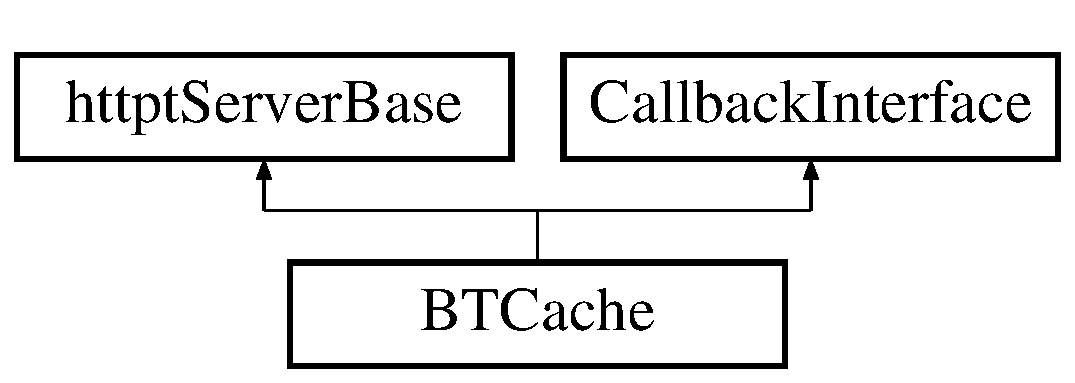
\includegraphics[height=2.000000cm]{classBTCache}
\end{center}
\end{figure}
\subsection*{Public Member Functions}
\begin{DoxyCompactItemize}
\item 
\hyperlink{classBTCache_a473a22048f77d193d17086f0d8cb3cc8}{B\+T\+Cache} ()
\item 
virtual \hyperlink{classBTCache_a8770b01f578dcca7a657d58a6d844f73}{$\sim$\+B\+T\+Cache} ()
\end{DoxyCompactItemize}
\subsection*{Protected Types}
\begin{DoxyCompactItemize}
\item 
typedef std\+::map$<$ T\+C\+P\+Socket $\ast$, c\+Packet $\ast$ $>$ \hyperlink{classBTCache_ac80b2a8f5787af11c89dbd05a187029e}{Client\+Map}
\item 
typedef std\+::set$<$ int $>$ \hyperlink{classBTCache_ae334281f1ee5074cc1d6e82b661b60e4}{T\+Set}
\end{DoxyCompactItemize}
\subsection*{Protected Member Functions}
\begin{DoxyCompactItemize}
\item 
virtual void \hyperlink{classBTCache_aab85cef7a8a821c2fca105264b97f6ac}{update\+Display} ()
\end{DoxyCompactItemize}
\subsection*{Protected Attributes}
\begin{DoxyCompactItemize}
\item 
httpt\+Controller $\ast$ \hyperlink{classBTCache_ac46f1f65119dfee3d87c5363101aa58b}{controller}
\item 
T\+C\+P\+Socket $\ast$ \hyperlink{classBTCache_ae3203717845093fb0a6e779f9d3d0b52}{listensocket}
\item 
T\+C\+P\+Socket\+Map \hyperlink{classBTCache_a43a311974146b2ef6bc69f6859d24e8e}{sock\+Collection}
\item 
T\+C\+P $\ast$ \hyperlink{classBTCache_ae867f4ad74074c00b641e390d3a9e372}{tcp}
\item 
c\+Module $\ast$ \hyperlink{classBTCache_a404b5d16a842340af5de6fab08181da9}{bt\+Statistics\+Module}
\item 
c\+Simple\+Module $\ast$ \hyperlink{classBTCache_a8299e74f2c743652ed3301c011656928}{bt\+Statistics}
\item 
\hyperlink{classBTCache_ac80b2a8f5787af11c89dbd05a187029e}{Client\+Map} \hyperlink{classBTCache_a27d62db096c4d09c449ecb10d8d19abf}{pending\+Requests}
\item 
unsigned long \hyperlink{classBTCache_a8f2f146c44949bcf78646c043caaae40}{server\+Sockets\+Broken}
\item 
unsigned long \hyperlink{classBTCache_a2b79808f6ff3b27684cebbb78d8801a6}{server\+Sockets\+Opened}
\item 
unsigned long \hyperlink{classBTCache_a59899107c3f728fe1f5703ad116b092c}{client\+Sockets\+Broken}
\item 
unsigned long \hyperlink{classBTCache_af68542d10296c40d603c98ee977a46d6}{client\+Sockets\+Opened}
\item 
unsigned long \hyperlink{classBTCache_ad1d45c4a6c3eb41f97723c052831c63f}{num\+Broken}
\item 
unsigned long \hyperlink{classBTCache_ada2e7c16bb0919521475b4fd6014cd80}{sockets\+Opened}
\item 
unsigned long \hyperlink{classBTCache_a14de443ddf388fb6b61381b5a881e099}{requests\+Received}
\item 
c\+Std\+Dev $\ast$ \hyperlink{classBTCache_a7432b26e77f5a8e3d5b910b5cbc179b3}{num\+Hits}
\item 
c\+Out\+Vector \hyperlink{classBTCache_a0ac804101085c06566877a36baa591e7}{num\+Hits\+\_\+vec}
\item 
c\+Std\+Dev $\ast$ \hyperlink{classBTCache_aeee4cfae3f278ceba5e900ab9c549f0e}{num\+Misses}
\item 
c\+Out\+Vector \hyperlink{classBTCache_ab687064d70f88dca7d7b5102fe2c1966}{num\+Misses\+\_\+vec}
\item 
Cache $\ast$ \hyperlink{classBTCache_ae126841ec3ca00972a328ff64a832e6a}{resource\+Cache}
\item 
int \hyperlink{classBTCache_a48ba69d513530368d210c5e97d19edbc}{hits}
\item 
int \hyperlink{classBTCache_a8ed86c3269e334690fb483a1884ee20a}{misses}
\item 
\hyperlink{classBTCache_ae334281f1ee5074cc1d6e82b661b60e4}{T\+Set} \hyperlink{classBTCache_a464a4dd8ca5b0313b24675deeb7fec6e}{server\+Connections}
\end{DoxyCompactItemize}


\subsection{Member Typedef Documentation}
\hypertarget{classBTCache_ac80b2a8f5787af11c89dbd05a187029e}{}\index{B\+T\+Cache@{B\+T\+Cache}!Client\+Map@{Client\+Map}}
\index{Client\+Map@{Client\+Map}!B\+T\+Cache@{B\+T\+Cache}}
\subsubsection[{Client\+Map}]{\setlength{\rightskip}{0pt plus 5cm}typedef std\+::map$<$T\+C\+P\+Socket$\ast$, c\+Packet$\ast$$>$ {\bf B\+T\+Cache\+::\+Client\+Map}\hspace{0.3cm}{\ttfamily [protected]}}\label{classBTCache_ac80b2a8f5787af11c89dbd05a187029e}
\hypertarget{classBTCache_ae334281f1ee5074cc1d6e82b661b60e4}{}\index{B\+T\+Cache@{B\+T\+Cache}!T\+Set@{T\+Set}}
\index{T\+Set@{T\+Set}!B\+T\+Cache@{B\+T\+Cache}}
\subsubsection[{T\+Set}]{\setlength{\rightskip}{0pt plus 5cm}typedef std\+::set$<$int$>$ {\bf B\+T\+Cache\+::\+T\+Set}\hspace{0.3cm}{\ttfamily [protected]}}\label{classBTCache_ae334281f1ee5074cc1d6e82b661b60e4}


\subsection{Constructor \& Destructor Documentation}
\hypertarget{classBTCache_a473a22048f77d193d17086f0d8cb3cc8}{}\index{B\+T\+Cache@{B\+T\+Cache}!B\+T\+Cache@{B\+T\+Cache}}
\index{B\+T\+Cache@{B\+T\+Cache}!B\+T\+Cache@{B\+T\+Cache}}
\subsubsection[{B\+T\+Cache()}]{\setlength{\rightskip}{0pt plus 5cm}B\+T\+Cache\+::\+B\+T\+Cache (
\begin{DoxyParamCaption}
{}
\end{DoxyParamCaption}
)}\label{classBTCache_a473a22048f77d193d17086f0d8cb3cc8}
\hypertarget{classBTCache_a8770b01f578dcca7a657d58a6d844f73}{}\index{B\+T\+Cache@{B\+T\+Cache}!````~B\+T\+Cache@{$\sim$\+B\+T\+Cache}}
\index{````~B\+T\+Cache@{$\sim$\+B\+T\+Cache}!B\+T\+Cache@{B\+T\+Cache}}
\subsubsection[{$\sim$\+B\+T\+Cache()}]{\setlength{\rightskip}{0pt plus 5cm}B\+T\+Cache\+::$\sim$\+B\+T\+Cache (
\begin{DoxyParamCaption}
{}
\end{DoxyParamCaption}
)\hspace{0.3cm}{\ttfamily [virtual]}}\label{classBTCache_a8770b01f578dcca7a657d58a6d844f73}


\subsection{Member Function Documentation}
\hypertarget{classBTCache_aab85cef7a8a821c2fca105264b97f6ac}{}\index{B\+T\+Cache@{B\+T\+Cache}!update\+Display@{update\+Display}}
\index{update\+Display@{update\+Display}!B\+T\+Cache@{B\+T\+Cache}}
\subsubsection[{update\+Display()}]{\setlength{\rightskip}{0pt plus 5cm}void B\+T\+Cache\+::update\+Display (
\begin{DoxyParamCaption}
{}
\end{DoxyParamCaption}
)\hspace{0.3cm}{\ttfamily [protected]}, {\ttfamily [virtual]}}\label{classBTCache_aab85cef7a8a821c2fca105264b97f6ac}


\subsection{Member Data Documentation}
\hypertarget{classBTCache_a8299e74f2c743652ed3301c011656928}{}\index{B\+T\+Cache@{B\+T\+Cache}!bt\+Statistics@{bt\+Statistics}}
\index{bt\+Statistics@{bt\+Statistics}!B\+T\+Cache@{B\+T\+Cache}}
\subsubsection[{bt\+Statistics}]{\setlength{\rightskip}{0pt plus 5cm}c\+Simple\+Module$\ast$ B\+T\+Cache\+::bt\+Statistics\hspace{0.3cm}{\ttfamily [protected]}}\label{classBTCache_a8299e74f2c743652ed3301c011656928}
\hypertarget{classBTCache_a404b5d16a842340af5de6fab08181da9}{}\index{B\+T\+Cache@{B\+T\+Cache}!bt\+Statistics\+Module@{bt\+Statistics\+Module}}
\index{bt\+Statistics\+Module@{bt\+Statistics\+Module}!B\+T\+Cache@{B\+T\+Cache}}
\subsubsection[{bt\+Statistics\+Module}]{\setlength{\rightskip}{0pt plus 5cm}c\+Module$\ast$ B\+T\+Cache\+::bt\+Statistics\+Module\hspace{0.3cm}{\ttfamily [protected]}}\label{classBTCache_a404b5d16a842340af5de6fab08181da9}
\hypertarget{classBTCache_a59899107c3f728fe1f5703ad116b092c}{}\index{B\+T\+Cache@{B\+T\+Cache}!client\+Sockets\+Broken@{client\+Sockets\+Broken}}
\index{client\+Sockets\+Broken@{client\+Sockets\+Broken}!B\+T\+Cache@{B\+T\+Cache}}
\subsubsection[{client\+Sockets\+Broken}]{\setlength{\rightskip}{0pt plus 5cm}unsigned long B\+T\+Cache\+::client\+Sockets\+Broken\hspace{0.3cm}{\ttfamily [protected]}}\label{classBTCache_a59899107c3f728fe1f5703ad116b092c}
\hypertarget{classBTCache_af68542d10296c40d603c98ee977a46d6}{}\index{B\+T\+Cache@{B\+T\+Cache}!client\+Sockets\+Opened@{client\+Sockets\+Opened}}
\index{client\+Sockets\+Opened@{client\+Sockets\+Opened}!B\+T\+Cache@{B\+T\+Cache}}
\subsubsection[{client\+Sockets\+Opened}]{\setlength{\rightskip}{0pt plus 5cm}unsigned long B\+T\+Cache\+::client\+Sockets\+Opened\hspace{0.3cm}{\ttfamily [protected]}}\label{classBTCache_af68542d10296c40d603c98ee977a46d6}
\hypertarget{classBTCache_ac46f1f65119dfee3d87c5363101aa58b}{}\index{B\+T\+Cache@{B\+T\+Cache}!controller@{controller}}
\index{controller@{controller}!B\+T\+Cache@{B\+T\+Cache}}
\subsubsection[{controller}]{\setlength{\rightskip}{0pt plus 5cm}httpt\+Controller$\ast$ B\+T\+Cache\+::controller\hspace{0.3cm}{\ttfamily [protected]}}\label{classBTCache_ac46f1f65119dfee3d87c5363101aa58b}
\hypertarget{classBTCache_a48ba69d513530368d210c5e97d19edbc}{}\index{B\+T\+Cache@{B\+T\+Cache}!hits@{hits}}
\index{hits@{hits}!B\+T\+Cache@{B\+T\+Cache}}
\subsubsection[{hits}]{\setlength{\rightskip}{0pt plus 5cm}int B\+T\+Cache\+::hits\hspace{0.3cm}{\ttfamily [protected]}}\label{classBTCache_a48ba69d513530368d210c5e97d19edbc}
\hypertarget{classBTCache_ae3203717845093fb0a6e779f9d3d0b52}{}\index{B\+T\+Cache@{B\+T\+Cache}!listensocket@{listensocket}}
\index{listensocket@{listensocket}!B\+T\+Cache@{B\+T\+Cache}}
\subsubsection[{listensocket}]{\setlength{\rightskip}{0pt plus 5cm}T\+C\+P\+Socket$\ast$ B\+T\+Cache\+::listensocket\hspace{0.3cm}{\ttfamily [protected]}}\label{classBTCache_ae3203717845093fb0a6e779f9d3d0b52}
\hypertarget{classBTCache_a8ed86c3269e334690fb483a1884ee20a}{}\index{B\+T\+Cache@{B\+T\+Cache}!misses@{misses}}
\index{misses@{misses}!B\+T\+Cache@{B\+T\+Cache}}
\subsubsection[{misses}]{\setlength{\rightskip}{0pt plus 5cm}int B\+T\+Cache\+::misses\hspace{0.3cm}{\ttfamily [protected]}}\label{classBTCache_a8ed86c3269e334690fb483a1884ee20a}
\hypertarget{classBTCache_ad1d45c4a6c3eb41f97723c052831c63f}{}\index{B\+T\+Cache@{B\+T\+Cache}!num\+Broken@{num\+Broken}}
\index{num\+Broken@{num\+Broken}!B\+T\+Cache@{B\+T\+Cache}}
\subsubsection[{num\+Broken}]{\setlength{\rightskip}{0pt plus 5cm}unsigned long B\+T\+Cache\+::num\+Broken\hspace{0.3cm}{\ttfamily [protected]}}\label{classBTCache_ad1d45c4a6c3eb41f97723c052831c63f}
\hypertarget{classBTCache_a7432b26e77f5a8e3d5b910b5cbc179b3}{}\index{B\+T\+Cache@{B\+T\+Cache}!num\+Hits@{num\+Hits}}
\index{num\+Hits@{num\+Hits}!B\+T\+Cache@{B\+T\+Cache}}
\subsubsection[{num\+Hits}]{\setlength{\rightskip}{0pt plus 5cm}c\+Std\+Dev$\ast$ B\+T\+Cache\+::num\+Hits\hspace{0.3cm}{\ttfamily [protected]}}\label{classBTCache_a7432b26e77f5a8e3d5b910b5cbc179b3}
\hypertarget{classBTCache_a0ac804101085c06566877a36baa591e7}{}\index{B\+T\+Cache@{B\+T\+Cache}!num\+Hits\+\_\+vec@{num\+Hits\+\_\+vec}}
\index{num\+Hits\+\_\+vec@{num\+Hits\+\_\+vec}!B\+T\+Cache@{B\+T\+Cache}}
\subsubsection[{num\+Hits\+\_\+vec}]{\setlength{\rightskip}{0pt plus 5cm}c\+Out\+Vector B\+T\+Cache\+::num\+Hits\+\_\+vec\hspace{0.3cm}{\ttfamily [protected]}}\label{classBTCache_a0ac804101085c06566877a36baa591e7}
\hypertarget{classBTCache_aeee4cfae3f278ceba5e900ab9c549f0e}{}\index{B\+T\+Cache@{B\+T\+Cache}!num\+Misses@{num\+Misses}}
\index{num\+Misses@{num\+Misses}!B\+T\+Cache@{B\+T\+Cache}}
\subsubsection[{num\+Misses}]{\setlength{\rightskip}{0pt plus 5cm}c\+Std\+Dev$\ast$ B\+T\+Cache\+::num\+Misses\hspace{0.3cm}{\ttfamily [protected]}}\label{classBTCache_aeee4cfae3f278ceba5e900ab9c549f0e}
\hypertarget{classBTCache_ab687064d70f88dca7d7b5102fe2c1966}{}\index{B\+T\+Cache@{B\+T\+Cache}!num\+Misses\+\_\+vec@{num\+Misses\+\_\+vec}}
\index{num\+Misses\+\_\+vec@{num\+Misses\+\_\+vec}!B\+T\+Cache@{B\+T\+Cache}}
\subsubsection[{num\+Misses\+\_\+vec}]{\setlength{\rightskip}{0pt plus 5cm}c\+Out\+Vector B\+T\+Cache\+::num\+Misses\+\_\+vec\hspace{0.3cm}{\ttfamily [protected]}}\label{classBTCache_ab687064d70f88dca7d7b5102fe2c1966}
\hypertarget{classBTCache_a27d62db096c4d09c449ecb10d8d19abf}{}\index{B\+T\+Cache@{B\+T\+Cache}!pending\+Requests@{pending\+Requests}}
\index{pending\+Requests@{pending\+Requests}!B\+T\+Cache@{B\+T\+Cache}}
\subsubsection[{pending\+Requests}]{\setlength{\rightskip}{0pt plus 5cm}{\bf Client\+Map} B\+T\+Cache\+::pending\+Requests\hspace{0.3cm}{\ttfamily [protected]}}\label{classBTCache_a27d62db096c4d09c449ecb10d8d19abf}
\hypertarget{classBTCache_a14de443ddf388fb6b61381b5a881e099}{}\index{B\+T\+Cache@{B\+T\+Cache}!requests\+Received@{requests\+Received}}
\index{requests\+Received@{requests\+Received}!B\+T\+Cache@{B\+T\+Cache}}
\subsubsection[{requests\+Received}]{\setlength{\rightskip}{0pt plus 5cm}unsigned long B\+T\+Cache\+::requests\+Received\hspace{0.3cm}{\ttfamily [protected]}}\label{classBTCache_a14de443ddf388fb6b61381b5a881e099}
\hypertarget{classBTCache_ae126841ec3ca00972a328ff64a832e6a}{}\index{B\+T\+Cache@{B\+T\+Cache}!resource\+Cache@{resource\+Cache}}
\index{resource\+Cache@{resource\+Cache}!B\+T\+Cache@{B\+T\+Cache}}
\subsubsection[{resource\+Cache}]{\setlength{\rightskip}{0pt plus 5cm}Cache$\ast$ B\+T\+Cache\+::resource\+Cache\hspace{0.3cm}{\ttfamily [protected]}}\label{classBTCache_ae126841ec3ca00972a328ff64a832e6a}
\hypertarget{classBTCache_a464a4dd8ca5b0313b24675deeb7fec6e}{}\index{B\+T\+Cache@{B\+T\+Cache}!server\+Connections@{server\+Connections}}
\index{server\+Connections@{server\+Connections}!B\+T\+Cache@{B\+T\+Cache}}
\subsubsection[{server\+Connections}]{\setlength{\rightskip}{0pt plus 5cm}{\bf T\+Set} B\+T\+Cache\+::server\+Connections\hspace{0.3cm}{\ttfamily [protected]}}\label{classBTCache_a464a4dd8ca5b0313b24675deeb7fec6e}
\hypertarget{classBTCache_a8f2f146c44949bcf78646c043caaae40}{}\index{B\+T\+Cache@{B\+T\+Cache}!server\+Sockets\+Broken@{server\+Sockets\+Broken}}
\index{server\+Sockets\+Broken@{server\+Sockets\+Broken}!B\+T\+Cache@{B\+T\+Cache}}
\subsubsection[{server\+Sockets\+Broken}]{\setlength{\rightskip}{0pt plus 5cm}unsigned long B\+T\+Cache\+::server\+Sockets\+Broken\hspace{0.3cm}{\ttfamily [protected]}}\label{classBTCache_a8f2f146c44949bcf78646c043caaae40}
\hypertarget{classBTCache_a2b79808f6ff3b27684cebbb78d8801a6}{}\index{B\+T\+Cache@{B\+T\+Cache}!server\+Sockets\+Opened@{server\+Sockets\+Opened}}
\index{server\+Sockets\+Opened@{server\+Sockets\+Opened}!B\+T\+Cache@{B\+T\+Cache}}
\subsubsection[{server\+Sockets\+Opened}]{\setlength{\rightskip}{0pt plus 5cm}unsigned long B\+T\+Cache\+::server\+Sockets\+Opened\hspace{0.3cm}{\ttfamily [protected]}}\label{classBTCache_a2b79808f6ff3b27684cebbb78d8801a6}
\hypertarget{classBTCache_a43a311974146b2ef6bc69f6859d24e8e}{}\index{B\+T\+Cache@{B\+T\+Cache}!sock\+Collection@{sock\+Collection}}
\index{sock\+Collection@{sock\+Collection}!B\+T\+Cache@{B\+T\+Cache}}
\subsubsection[{sock\+Collection}]{\setlength{\rightskip}{0pt plus 5cm}T\+C\+P\+Socket\+Map B\+T\+Cache\+::sock\+Collection\hspace{0.3cm}{\ttfamily [protected]}}\label{classBTCache_a43a311974146b2ef6bc69f6859d24e8e}
\hypertarget{classBTCache_ada2e7c16bb0919521475b4fd6014cd80}{}\index{B\+T\+Cache@{B\+T\+Cache}!sockets\+Opened@{sockets\+Opened}}
\index{sockets\+Opened@{sockets\+Opened}!B\+T\+Cache@{B\+T\+Cache}}
\subsubsection[{sockets\+Opened}]{\setlength{\rightskip}{0pt plus 5cm}unsigned long B\+T\+Cache\+::sockets\+Opened\hspace{0.3cm}{\ttfamily [protected]}}\label{classBTCache_ada2e7c16bb0919521475b4fd6014cd80}
\hypertarget{classBTCache_ae867f4ad74074c00b641e390d3a9e372}{}\index{B\+T\+Cache@{B\+T\+Cache}!tcp@{tcp}}
\index{tcp@{tcp}!B\+T\+Cache@{B\+T\+Cache}}
\subsubsection[{tcp}]{\setlength{\rightskip}{0pt plus 5cm}T\+C\+P$\ast$ B\+T\+Cache\+::tcp\hspace{0.3cm}{\ttfamily [protected]}}\label{classBTCache_ae867f4ad74074c00b641e390d3a9e372}


The documentation for this class was generated from the following files\+:\begin{DoxyCompactItemize}
\item 
\hyperlink{BTCache_8h}{B\+T\+Cache.\+h}\item 
\hyperlink{BTCache_8cc}{B\+T\+Cache.\+cc}\end{DoxyCompactItemize}

\hypertarget{classBTHaveMsg}{}\section{B\+T\+Have\+Msg Class Reference}
\label{classBTHaveMsg}\index{B\+T\+Have\+Msg@{B\+T\+Have\+Msg}}


{\ttfamily \#include $<$B\+T\+Peer\+Wire\+Msg\+\_\+m.\+h$>$}

Inheritance diagram for B\+T\+Have\+Msg\+:\begin{figure}[H]
\begin{center}
\leavevmode
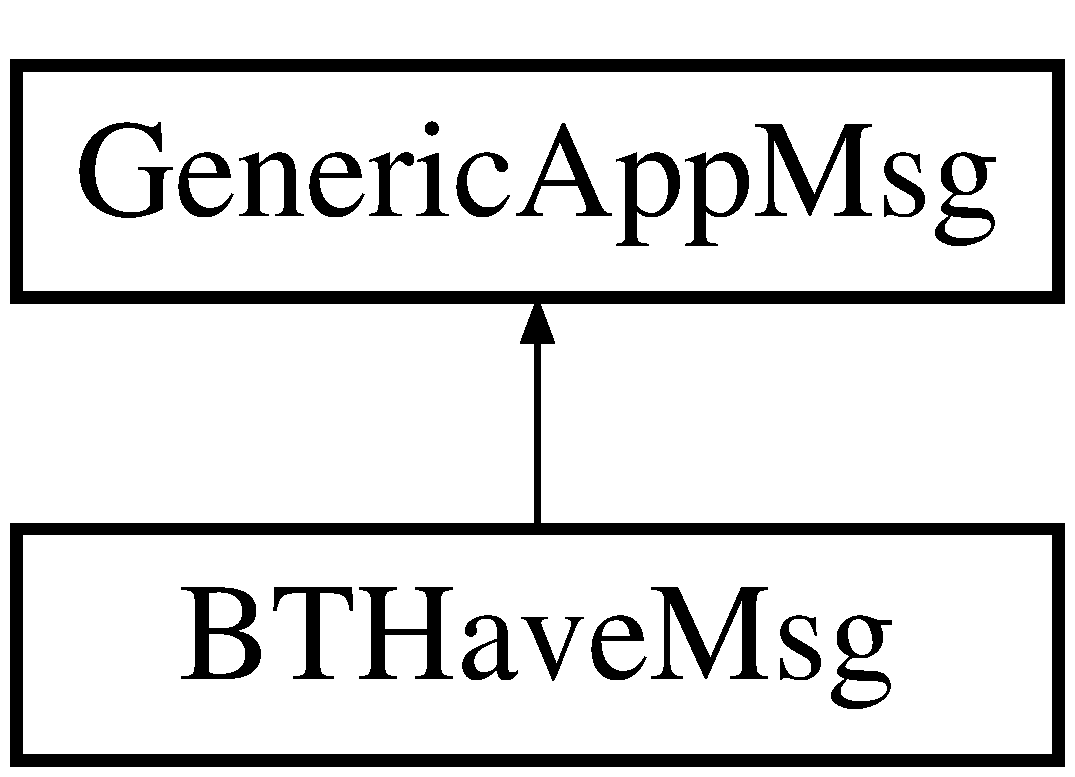
\includegraphics[height=2.000000cm]{classBTHaveMsg}
\end{center}
\end{figure}
\subsection*{Public Member Functions}
\begin{DoxyCompactItemize}
\item 
\hyperlink{classBTHaveMsg_ad698bdad1ba35798b5e2b3680eccb48a}{B\+T\+Have\+Msg} (const char $\ast$name=N\+U\+L\+L, int kind=0)
\item 
\hyperlink{classBTHaveMsg_ad6fbc684e278c80379a62d5f7323f797}{B\+T\+Have\+Msg} (const \hyperlink{classBTHaveMsg}{B\+T\+Have\+Msg} \&other)
\item 
virtual \hyperlink{classBTHaveMsg_a6bcd9e02e152c9e225bcea3626ca51ba}{$\sim$\+B\+T\+Have\+Msg} ()
\item 
\hyperlink{classBTHaveMsg}{B\+T\+Have\+Msg} \& \hyperlink{classBTHaveMsg_a272493bb474b120d81994a2e5c21f60b}{operator=} (const \hyperlink{classBTHaveMsg}{B\+T\+Have\+Msg} \&other)
\item 
virtual \hyperlink{classBTHaveMsg}{B\+T\+Have\+Msg} $\ast$ \hyperlink{classBTHaveMsg_adb7135f65e0c795d57269863267a06f5}{dup} () const 
\item 
virtual void \hyperlink{classBTHaveMsg_a845818586977d3dea95c9da85f2e8b2d}{parsim\+Pack} (c\+Comm\+Buffer $\ast$b)
\item 
virtual void \hyperlink{classBTHaveMsg_ab616fdeb1fa6886ec873082fd23d786d}{parsim\+Unpack} (c\+Comm\+Buffer $\ast$b)
\item 
virtual int \hyperlink{classBTHaveMsg_a4635462d5b8b5f267f9c34f474c2da06}{length\+\_\+prefix} () const 
\item 
virtual void \hyperlink{classBTHaveMsg_add034dad6ba5390be3a0e282da86ed73}{set\+Length\+\_\+prefix} (int \hyperlink{classBTHaveMsg_a3d41affb383127b621ed0674a69bc77e}{length\+\_\+prefix\+\_\+var})
\item 
virtual unsigned short \hyperlink{classBTHaveMsg_a8cd968be4ae5602f710655a9af0a7188}{I\+D} () const 
\item 
virtual void \hyperlink{classBTHaveMsg_a34d1913993ccca96cfd28a37bdbf3d84}{set\+I\+D} (unsigned short \hyperlink{classBTHaveMsg_a64e557f1acff2867bdd000a2cd71a9d7}{I\+D\+\_\+var})
\item 
virtual int \hyperlink{classBTHaveMsg_ae19164ccec7366fdc1edfed885369a61}{index} () const 
\item 
virtual void \hyperlink{classBTHaveMsg_a3f2f76800dfa7691bcfaf8444bc6e50a}{set\+Index} (int \hyperlink{classBTHaveMsg_a0cc4163cbb7ced674444b8fbc897327f}{index\+\_\+var})
\end{DoxyCompactItemize}
\subsection*{Protected Member Functions}
\begin{DoxyCompactItemize}
\item 
bool \hyperlink{classBTHaveMsg_ac4f8fd8f890666538356ba29a3564808}{operator==} (const \hyperlink{classBTHaveMsg}{B\+T\+Have\+Msg} \&)
\end{DoxyCompactItemize}
\subsection*{Protected Attributes}
\begin{DoxyCompactItemize}
\item 
int \hyperlink{classBTHaveMsg_a3d41affb383127b621ed0674a69bc77e}{length\+\_\+prefix\+\_\+var}
\item 
unsigned short \hyperlink{classBTHaveMsg_a64e557f1acff2867bdd000a2cd71a9d7}{I\+D\+\_\+var}
\item 
int \hyperlink{classBTHaveMsg_a0cc4163cbb7ced674444b8fbc897327f}{index\+\_\+var}
\end{DoxyCompactItemize}


\subsection{Constructor \& Destructor Documentation}
\hypertarget{classBTHaveMsg_ad698bdad1ba35798b5e2b3680eccb48a}{}\index{B\+T\+Have\+Msg@{B\+T\+Have\+Msg}!B\+T\+Have\+Msg@{B\+T\+Have\+Msg}}
\index{B\+T\+Have\+Msg@{B\+T\+Have\+Msg}!B\+T\+Have\+Msg@{B\+T\+Have\+Msg}}
\subsubsection[{B\+T\+Have\+Msg(const char $\ast$name=\+N\+U\+L\+L, int kind=0)}]{\setlength{\rightskip}{0pt plus 5cm}B\+T\+Have\+Msg\+::\+B\+T\+Have\+Msg (
\begin{DoxyParamCaption}
\item[{const char $\ast$}]{name = {\ttfamily NULL}, }
\item[{int}]{kind = {\ttfamily 0}}
\end{DoxyParamCaption}
)}\label{classBTHaveMsg_ad698bdad1ba35798b5e2b3680eccb48a}
\hypertarget{classBTHaveMsg_ad6fbc684e278c80379a62d5f7323f797}{}\index{B\+T\+Have\+Msg@{B\+T\+Have\+Msg}!B\+T\+Have\+Msg@{B\+T\+Have\+Msg}}
\index{B\+T\+Have\+Msg@{B\+T\+Have\+Msg}!B\+T\+Have\+Msg@{B\+T\+Have\+Msg}}
\subsubsection[{B\+T\+Have\+Msg(const B\+T\+Have\+Msg \&other)}]{\setlength{\rightskip}{0pt plus 5cm}B\+T\+Have\+Msg\+::\+B\+T\+Have\+Msg (
\begin{DoxyParamCaption}
\item[{const {\bf B\+T\+Have\+Msg} \&}]{other}
\end{DoxyParamCaption}
)}\label{classBTHaveMsg_ad6fbc684e278c80379a62d5f7323f797}
\hypertarget{classBTHaveMsg_a6bcd9e02e152c9e225bcea3626ca51ba}{}\index{B\+T\+Have\+Msg@{B\+T\+Have\+Msg}!````~B\+T\+Have\+Msg@{$\sim$\+B\+T\+Have\+Msg}}
\index{````~B\+T\+Have\+Msg@{$\sim$\+B\+T\+Have\+Msg}!B\+T\+Have\+Msg@{B\+T\+Have\+Msg}}
\subsubsection[{$\sim$\+B\+T\+Have\+Msg()}]{\setlength{\rightskip}{0pt plus 5cm}B\+T\+Have\+Msg\+::$\sim$\+B\+T\+Have\+Msg (
\begin{DoxyParamCaption}
{}
\end{DoxyParamCaption}
)\hspace{0.3cm}{\ttfamily [virtual]}}\label{classBTHaveMsg_a6bcd9e02e152c9e225bcea3626ca51ba}


\subsection{Member Function Documentation}
\hypertarget{classBTHaveMsg_adb7135f65e0c795d57269863267a06f5}{}\index{B\+T\+Have\+Msg@{B\+T\+Have\+Msg}!dup@{dup}}
\index{dup@{dup}!B\+T\+Have\+Msg@{B\+T\+Have\+Msg}}
\subsubsection[{dup() const }]{\setlength{\rightskip}{0pt plus 5cm}virtual {\bf B\+T\+Have\+Msg}$\ast$ B\+T\+Have\+Msg\+::dup (
\begin{DoxyParamCaption}
{}
\end{DoxyParamCaption}
) const\hspace{0.3cm}{\ttfamily [inline]}, {\ttfamily [virtual]}}\label{classBTHaveMsg_adb7135f65e0c795d57269863267a06f5}
\hypertarget{classBTHaveMsg_a8cd968be4ae5602f710655a9af0a7188}{}\index{B\+T\+Have\+Msg@{B\+T\+Have\+Msg}!I\+D@{I\+D}}
\index{I\+D@{I\+D}!B\+T\+Have\+Msg@{B\+T\+Have\+Msg}}
\subsubsection[{I\+D() const }]{\setlength{\rightskip}{0pt plus 5cm}unsigned short B\+T\+Have\+Msg\+::\+I\+D (
\begin{DoxyParamCaption}
{}
\end{DoxyParamCaption}
) const\hspace{0.3cm}{\ttfamily [virtual]}}\label{classBTHaveMsg_a8cd968be4ae5602f710655a9af0a7188}
\hypertarget{classBTHaveMsg_ae19164ccec7366fdc1edfed885369a61}{}\index{B\+T\+Have\+Msg@{B\+T\+Have\+Msg}!index@{index}}
\index{index@{index}!B\+T\+Have\+Msg@{B\+T\+Have\+Msg}}
\subsubsection[{index() const }]{\setlength{\rightskip}{0pt plus 5cm}int B\+T\+Have\+Msg\+::index (
\begin{DoxyParamCaption}
{}
\end{DoxyParamCaption}
) const\hspace{0.3cm}{\ttfamily [virtual]}}\label{classBTHaveMsg_ae19164ccec7366fdc1edfed885369a61}
\hypertarget{classBTHaveMsg_a4635462d5b8b5f267f9c34f474c2da06}{}\index{B\+T\+Have\+Msg@{B\+T\+Have\+Msg}!length\+\_\+prefix@{length\+\_\+prefix}}
\index{length\+\_\+prefix@{length\+\_\+prefix}!B\+T\+Have\+Msg@{B\+T\+Have\+Msg}}
\subsubsection[{length\+\_\+prefix() const }]{\setlength{\rightskip}{0pt plus 5cm}int B\+T\+Have\+Msg\+::length\+\_\+prefix (
\begin{DoxyParamCaption}
{}
\end{DoxyParamCaption}
) const\hspace{0.3cm}{\ttfamily [virtual]}}\label{classBTHaveMsg_a4635462d5b8b5f267f9c34f474c2da06}
\hypertarget{classBTHaveMsg_a272493bb474b120d81994a2e5c21f60b}{}\index{B\+T\+Have\+Msg@{B\+T\+Have\+Msg}!operator=@{operator=}}
\index{operator=@{operator=}!B\+T\+Have\+Msg@{B\+T\+Have\+Msg}}
\subsubsection[{operator=(const B\+T\+Have\+Msg \&other)}]{\setlength{\rightskip}{0pt plus 5cm}{\bf B\+T\+Have\+Msg} \& B\+T\+Have\+Msg\+::operator= (
\begin{DoxyParamCaption}
\item[{const {\bf B\+T\+Have\+Msg} \&}]{other}
\end{DoxyParamCaption}
)}\label{classBTHaveMsg_a272493bb474b120d81994a2e5c21f60b}
\hypertarget{classBTHaveMsg_ac4f8fd8f890666538356ba29a3564808}{}\index{B\+T\+Have\+Msg@{B\+T\+Have\+Msg}!operator==@{operator==}}
\index{operator==@{operator==}!B\+T\+Have\+Msg@{B\+T\+Have\+Msg}}
\subsubsection[{operator==(const B\+T\+Have\+Msg \&)}]{\setlength{\rightskip}{0pt plus 5cm}bool B\+T\+Have\+Msg\+::operator== (
\begin{DoxyParamCaption}
\item[{const {\bf B\+T\+Have\+Msg} \&}]{}
\end{DoxyParamCaption}
)\hspace{0.3cm}{\ttfamily [protected]}}\label{classBTHaveMsg_ac4f8fd8f890666538356ba29a3564808}
\hypertarget{classBTHaveMsg_a845818586977d3dea95c9da85f2e8b2d}{}\index{B\+T\+Have\+Msg@{B\+T\+Have\+Msg}!parsim\+Pack@{parsim\+Pack}}
\index{parsim\+Pack@{parsim\+Pack}!B\+T\+Have\+Msg@{B\+T\+Have\+Msg}}
\subsubsection[{parsim\+Pack(c\+Comm\+Buffer $\ast$b)}]{\setlength{\rightskip}{0pt plus 5cm}void B\+T\+Have\+Msg\+::parsim\+Pack (
\begin{DoxyParamCaption}
\item[{c\+Comm\+Buffer $\ast$}]{b}
\end{DoxyParamCaption}
)\hspace{0.3cm}{\ttfamily [virtual]}}\label{classBTHaveMsg_a845818586977d3dea95c9da85f2e8b2d}
\hypertarget{classBTHaveMsg_ab616fdeb1fa6886ec873082fd23d786d}{}\index{B\+T\+Have\+Msg@{B\+T\+Have\+Msg}!parsim\+Unpack@{parsim\+Unpack}}
\index{parsim\+Unpack@{parsim\+Unpack}!B\+T\+Have\+Msg@{B\+T\+Have\+Msg}}
\subsubsection[{parsim\+Unpack(c\+Comm\+Buffer $\ast$b)}]{\setlength{\rightskip}{0pt plus 5cm}void B\+T\+Have\+Msg\+::parsim\+Unpack (
\begin{DoxyParamCaption}
\item[{c\+Comm\+Buffer $\ast$}]{b}
\end{DoxyParamCaption}
)\hspace{0.3cm}{\ttfamily [virtual]}}\label{classBTHaveMsg_ab616fdeb1fa6886ec873082fd23d786d}
\hypertarget{classBTHaveMsg_a34d1913993ccca96cfd28a37bdbf3d84}{}\index{B\+T\+Have\+Msg@{B\+T\+Have\+Msg}!set\+I\+D@{set\+I\+D}}
\index{set\+I\+D@{set\+I\+D}!B\+T\+Have\+Msg@{B\+T\+Have\+Msg}}
\subsubsection[{set\+I\+D(unsigned short I\+D\+\_\+var)}]{\setlength{\rightskip}{0pt plus 5cm}void B\+T\+Have\+Msg\+::set\+I\+D (
\begin{DoxyParamCaption}
\item[{unsigned short}]{I\+D\+\_\+var}
\end{DoxyParamCaption}
)\hspace{0.3cm}{\ttfamily [virtual]}}\label{classBTHaveMsg_a34d1913993ccca96cfd28a37bdbf3d84}
\hypertarget{classBTHaveMsg_a3f2f76800dfa7691bcfaf8444bc6e50a}{}\index{B\+T\+Have\+Msg@{B\+T\+Have\+Msg}!set\+Index@{set\+Index}}
\index{set\+Index@{set\+Index}!B\+T\+Have\+Msg@{B\+T\+Have\+Msg}}
\subsubsection[{set\+Index(int index\+\_\+var)}]{\setlength{\rightskip}{0pt plus 5cm}void B\+T\+Have\+Msg\+::set\+Index (
\begin{DoxyParamCaption}
\item[{int}]{index\+\_\+var}
\end{DoxyParamCaption}
)\hspace{0.3cm}{\ttfamily [virtual]}}\label{classBTHaveMsg_a3f2f76800dfa7691bcfaf8444bc6e50a}
\hypertarget{classBTHaveMsg_add034dad6ba5390be3a0e282da86ed73}{}\index{B\+T\+Have\+Msg@{B\+T\+Have\+Msg}!set\+Length\+\_\+prefix@{set\+Length\+\_\+prefix}}
\index{set\+Length\+\_\+prefix@{set\+Length\+\_\+prefix}!B\+T\+Have\+Msg@{B\+T\+Have\+Msg}}
\subsubsection[{set\+Length\+\_\+prefix(int length\+\_\+prefix\+\_\+var)}]{\setlength{\rightskip}{0pt plus 5cm}void B\+T\+Have\+Msg\+::set\+Length\+\_\+prefix (
\begin{DoxyParamCaption}
\item[{int}]{length\+\_\+prefix\+\_\+var}
\end{DoxyParamCaption}
)\hspace{0.3cm}{\ttfamily [virtual]}}\label{classBTHaveMsg_add034dad6ba5390be3a0e282da86ed73}


\subsection{Member Data Documentation}
\hypertarget{classBTHaveMsg_a64e557f1acff2867bdd000a2cd71a9d7}{}\index{B\+T\+Have\+Msg@{B\+T\+Have\+Msg}!I\+D\+\_\+var@{I\+D\+\_\+var}}
\index{I\+D\+\_\+var@{I\+D\+\_\+var}!B\+T\+Have\+Msg@{B\+T\+Have\+Msg}}
\subsubsection[{I\+D\+\_\+var}]{\setlength{\rightskip}{0pt plus 5cm}unsigned short B\+T\+Have\+Msg\+::\+I\+D\+\_\+var\hspace{0.3cm}{\ttfamily [protected]}}\label{classBTHaveMsg_a64e557f1acff2867bdd000a2cd71a9d7}
\hypertarget{classBTHaveMsg_a0cc4163cbb7ced674444b8fbc897327f}{}\index{B\+T\+Have\+Msg@{B\+T\+Have\+Msg}!index\+\_\+var@{index\+\_\+var}}
\index{index\+\_\+var@{index\+\_\+var}!B\+T\+Have\+Msg@{B\+T\+Have\+Msg}}
\subsubsection[{index\+\_\+var}]{\setlength{\rightskip}{0pt plus 5cm}int B\+T\+Have\+Msg\+::index\+\_\+var\hspace{0.3cm}{\ttfamily [protected]}}\label{classBTHaveMsg_a0cc4163cbb7ced674444b8fbc897327f}
\hypertarget{classBTHaveMsg_a3d41affb383127b621ed0674a69bc77e}{}\index{B\+T\+Have\+Msg@{B\+T\+Have\+Msg}!length\+\_\+prefix\+\_\+var@{length\+\_\+prefix\+\_\+var}}
\index{length\+\_\+prefix\+\_\+var@{length\+\_\+prefix\+\_\+var}!B\+T\+Have\+Msg@{B\+T\+Have\+Msg}}
\subsubsection[{length\+\_\+prefix\+\_\+var}]{\setlength{\rightskip}{0pt plus 5cm}int B\+T\+Have\+Msg\+::length\+\_\+prefix\+\_\+var\hspace{0.3cm}{\ttfamily [protected]}}\label{classBTHaveMsg_a3d41affb383127b621ed0674a69bc77e}


The documentation for this class was generated from the following files\+:\begin{DoxyCompactItemize}
\item 
\hyperlink{BTPeerWireMsg__m_8h}{B\+T\+Peer\+Wire\+Msg\+\_\+m.\+h}\item 
\hyperlink{BTPeerWireMsg__m_8cc}{B\+T\+Peer\+Wire\+Msg\+\_\+m.\+cc}\end{DoxyCompactItemize}

\hypertarget{classBTHaveMsgDescriptor}{}\section{B\+T\+Have\+Msg\+Descriptor Class Reference}
\label{classBTHaveMsgDescriptor}\index{B\+T\+Have\+Msg\+Descriptor@{B\+T\+Have\+Msg\+Descriptor}}
Inheritance diagram for B\+T\+Have\+Msg\+Descriptor\+:\begin{figure}[H]
\begin{center}
\leavevmode
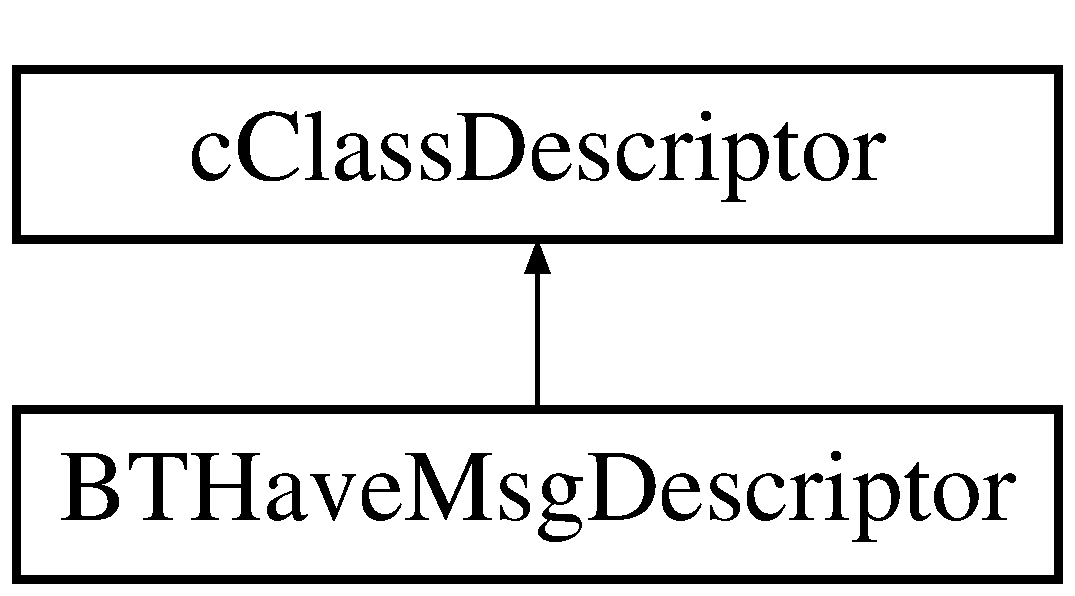
\includegraphics[height=2.000000cm]{classBTHaveMsgDescriptor}
\end{center}
\end{figure}
\subsection*{Public Member Functions}
\begin{DoxyCompactItemize}
\item 
\hyperlink{classBTHaveMsgDescriptor_a47122cfe2da1fc3c7819a175b5518201}{B\+T\+Have\+Msg\+Descriptor} ()
\item 
virtual \hyperlink{classBTHaveMsgDescriptor_a99c4061e220b597aaf145a0df7e28451}{$\sim$\+B\+T\+Have\+Msg\+Descriptor} ()
\item 
virtual bool \hyperlink{classBTHaveMsgDescriptor_a6e0cdbefa40e5cad291dacba394dbde3}{does\+Support} (c\+Object $\ast$obj) const 
\item 
virtual const char $\ast$ \hyperlink{classBTHaveMsgDescriptor_aa0d67607845765dd784042b2ab545358}{get\+Property} (const char $\ast$propertyname) const 
\item 
virtual int \hyperlink{classBTHaveMsgDescriptor_a1a8a41164b0394edc137cfb3152216cd}{get\+Field\+Count} (void $\ast$object) const 
\item 
virtual const char $\ast$ \hyperlink{classBTHaveMsgDescriptor_ad6049591e96cf93920d09770796b6516}{get\+Field\+Name} (void $\ast$object, int field) const 
\item 
virtual int \hyperlink{classBTHaveMsgDescriptor_a9d240eeed7cb467614a992206e1eb0d8}{find\+Field} (void $\ast$object, const char $\ast$field\+Name) const 
\item 
virtual unsigned int \hyperlink{classBTHaveMsgDescriptor_acff1f15e67ce27c82b773f3eb2361bb5}{get\+Field\+Type\+Flags} (void $\ast$object, int field) const 
\item 
virtual const char $\ast$ \hyperlink{classBTHaveMsgDescriptor_adb26434199e3bdc22f5451328dd42d32}{get\+Field\+Type\+String} (void $\ast$object, int field) const 
\item 
virtual const char $\ast$ \hyperlink{classBTHaveMsgDescriptor_a550a5202ddc41e8221c9ac520ffb5e5d}{get\+Field\+Property} (void $\ast$object, int field, const char $\ast$propertyname) const 
\item 
virtual int \hyperlink{classBTHaveMsgDescriptor_ab697b1c15128aad322df05a176e29d50}{get\+Array\+Size} (void $\ast$object, int field) const 
\item 
virtual std\+::string \hyperlink{classBTHaveMsgDescriptor_adb607bc085f1a234baf538ddc32f4ea5}{get\+Field\+As\+String} (void $\ast$object, int field, int i) const 
\item 
virtual bool \hyperlink{classBTHaveMsgDescriptor_ab9dd0f93b3f475afc26618aaf148d829}{set\+Field\+As\+String} (void $\ast$object, int field, int i, const char $\ast$value) const 
\item 
virtual const char $\ast$ \hyperlink{classBTHaveMsgDescriptor_a349e7c07a026e15dda29968c8dae8234}{get\+Field\+Struct\+Name} (void $\ast$object, int field) const 
\item 
virtual void $\ast$ \hyperlink{classBTHaveMsgDescriptor_a8ae12b16db8ffb8b2b82f116b7998ddd}{get\+Field\+Struct\+Pointer} (void $\ast$object, int field, int i) const 
\end{DoxyCompactItemize}


\subsection{Constructor \& Destructor Documentation}
\hypertarget{classBTHaveMsgDescriptor_a47122cfe2da1fc3c7819a175b5518201}{}\index{B\+T\+Have\+Msg\+Descriptor@{B\+T\+Have\+Msg\+Descriptor}!B\+T\+Have\+Msg\+Descriptor@{B\+T\+Have\+Msg\+Descriptor}}
\index{B\+T\+Have\+Msg\+Descriptor@{B\+T\+Have\+Msg\+Descriptor}!B\+T\+Have\+Msg\+Descriptor@{B\+T\+Have\+Msg\+Descriptor}}
\subsubsection[{B\+T\+Have\+Msg\+Descriptor()}]{\setlength{\rightskip}{0pt plus 5cm}B\+T\+Have\+Msg\+Descriptor\+::\+B\+T\+Have\+Msg\+Descriptor (
\begin{DoxyParamCaption}
{}
\end{DoxyParamCaption}
)}\label{classBTHaveMsgDescriptor_a47122cfe2da1fc3c7819a175b5518201}
\hypertarget{classBTHaveMsgDescriptor_a99c4061e220b597aaf145a0df7e28451}{}\index{B\+T\+Have\+Msg\+Descriptor@{B\+T\+Have\+Msg\+Descriptor}!````~B\+T\+Have\+Msg\+Descriptor@{$\sim$\+B\+T\+Have\+Msg\+Descriptor}}
\index{````~B\+T\+Have\+Msg\+Descriptor@{$\sim$\+B\+T\+Have\+Msg\+Descriptor}!B\+T\+Have\+Msg\+Descriptor@{B\+T\+Have\+Msg\+Descriptor}}
\subsubsection[{$\sim$\+B\+T\+Have\+Msg\+Descriptor()}]{\setlength{\rightskip}{0pt plus 5cm}B\+T\+Have\+Msg\+Descriptor\+::$\sim$\+B\+T\+Have\+Msg\+Descriptor (
\begin{DoxyParamCaption}
{}
\end{DoxyParamCaption}
)\hspace{0.3cm}{\ttfamily [virtual]}}\label{classBTHaveMsgDescriptor_a99c4061e220b597aaf145a0df7e28451}


\subsection{Member Function Documentation}
\hypertarget{classBTHaveMsgDescriptor_a6e0cdbefa40e5cad291dacba394dbde3}{}\index{B\+T\+Have\+Msg\+Descriptor@{B\+T\+Have\+Msg\+Descriptor}!does\+Support@{does\+Support}}
\index{does\+Support@{does\+Support}!B\+T\+Have\+Msg\+Descriptor@{B\+T\+Have\+Msg\+Descriptor}}
\subsubsection[{does\+Support(c\+Object $\ast$obj) const }]{\setlength{\rightskip}{0pt plus 5cm}bool B\+T\+Have\+Msg\+Descriptor\+::does\+Support (
\begin{DoxyParamCaption}
\item[{c\+Object $\ast$}]{obj}
\end{DoxyParamCaption}
) const\hspace{0.3cm}{\ttfamily [virtual]}}\label{classBTHaveMsgDescriptor_a6e0cdbefa40e5cad291dacba394dbde3}
\hypertarget{classBTHaveMsgDescriptor_a9d240eeed7cb467614a992206e1eb0d8}{}\index{B\+T\+Have\+Msg\+Descriptor@{B\+T\+Have\+Msg\+Descriptor}!find\+Field@{find\+Field}}
\index{find\+Field@{find\+Field}!B\+T\+Have\+Msg\+Descriptor@{B\+T\+Have\+Msg\+Descriptor}}
\subsubsection[{find\+Field(void $\ast$object, const char $\ast$field\+Name) const }]{\setlength{\rightskip}{0pt plus 5cm}int B\+T\+Have\+Msg\+Descriptor\+::find\+Field (
\begin{DoxyParamCaption}
\item[{void $\ast$}]{object, }
\item[{const char $\ast$}]{field\+Name}
\end{DoxyParamCaption}
) const\hspace{0.3cm}{\ttfamily [virtual]}}\label{classBTHaveMsgDescriptor_a9d240eeed7cb467614a992206e1eb0d8}
\hypertarget{classBTHaveMsgDescriptor_ab697b1c15128aad322df05a176e29d50}{}\index{B\+T\+Have\+Msg\+Descriptor@{B\+T\+Have\+Msg\+Descriptor}!get\+Array\+Size@{get\+Array\+Size}}
\index{get\+Array\+Size@{get\+Array\+Size}!B\+T\+Have\+Msg\+Descriptor@{B\+T\+Have\+Msg\+Descriptor}}
\subsubsection[{get\+Array\+Size(void $\ast$object, int field) const }]{\setlength{\rightskip}{0pt plus 5cm}int B\+T\+Have\+Msg\+Descriptor\+::get\+Array\+Size (
\begin{DoxyParamCaption}
\item[{void $\ast$}]{object, }
\item[{int}]{field}
\end{DoxyParamCaption}
) const\hspace{0.3cm}{\ttfamily [virtual]}}\label{classBTHaveMsgDescriptor_ab697b1c15128aad322df05a176e29d50}
\hypertarget{classBTHaveMsgDescriptor_adb607bc085f1a234baf538ddc32f4ea5}{}\index{B\+T\+Have\+Msg\+Descriptor@{B\+T\+Have\+Msg\+Descriptor}!get\+Field\+As\+String@{get\+Field\+As\+String}}
\index{get\+Field\+As\+String@{get\+Field\+As\+String}!B\+T\+Have\+Msg\+Descriptor@{B\+T\+Have\+Msg\+Descriptor}}
\subsubsection[{get\+Field\+As\+String(void $\ast$object, int field, int i) const }]{\setlength{\rightskip}{0pt plus 5cm}std\+::string B\+T\+Have\+Msg\+Descriptor\+::get\+Field\+As\+String (
\begin{DoxyParamCaption}
\item[{void $\ast$}]{object, }
\item[{int}]{field, }
\item[{int}]{i}
\end{DoxyParamCaption}
) const\hspace{0.3cm}{\ttfamily [virtual]}}\label{classBTHaveMsgDescriptor_adb607bc085f1a234baf538ddc32f4ea5}
\hypertarget{classBTHaveMsgDescriptor_a1a8a41164b0394edc137cfb3152216cd}{}\index{B\+T\+Have\+Msg\+Descriptor@{B\+T\+Have\+Msg\+Descriptor}!get\+Field\+Count@{get\+Field\+Count}}
\index{get\+Field\+Count@{get\+Field\+Count}!B\+T\+Have\+Msg\+Descriptor@{B\+T\+Have\+Msg\+Descriptor}}
\subsubsection[{get\+Field\+Count(void $\ast$object) const }]{\setlength{\rightskip}{0pt plus 5cm}int B\+T\+Have\+Msg\+Descriptor\+::get\+Field\+Count (
\begin{DoxyParamCaption}
\item[{void $\ast$}]{object}
\end{DoxyParamCaption}
) const\hspace{0.3cm}{\ttfamily [virtual]}}\label{classBTHaveMsgDescriptor_a1a8a41164b0394edc137cfb3152216cd}
\hypertarget{classBTHaveMsgDescriptor_ad6049591e96cf93920d09770796b6516}{}\index{B\+T\+Have\+Msg\+Descriptor@{B\+T\+Have\+Msg\+Descriptor}!get\+Field\+Name@{get\+Field\+Name}}
\index{get\+Field\+Name@{get\+Field\+Name}!B\+T\+Have\+Msg\+Descriptor@{B\+T\+Have\+Msg\+Descriptor}}
\subsubsection[{get\+Field\+Name(void $\ast$object, int field) const }]{\setlength{\rightskip}{0pt plus 5cm}const char $\ast$ B\+T\+Have\+Msg\+Descriptor\+::get\+Field\+Name (
\begin{DoxyParamCaption}
\item[{void $\ast$}]{object, }
\item[{int}]{field}
\end{DoxyParamCaption}
) const\hspace{0.3cm}{\ttfamily [virtual]}}\label{classBTHaveMsgDescriptor_ad6049591e96cf93920d09770796b6516}
\hypertarget{classBTHaveMsgDescriptor_a550a5202ddc41e8221c9ac520ffb5e5d}{}\index{B\+T\+Have\+Msg\+Descriptor@{B\+T\+Have\+Msg\+Descriptor}!get\+Field\+Property@{get\+Field\+Property}}
\index{get\+Field\+Property@{get\+Field\+Property}!B\+T\+Have\+Msg\+Descriptor@{B\+T\+Have\+Msg\+Descriptor}}
\subsubsection[{get\+Field\+Property(void $\ast$object, int field, const char $\ast$propertyname) const }]{\setlength{\rightskip}{0pt plus 5cm}const char $\ast$ B\+T\+Have\+Msg\+Descriptor\+::get\+Field\+Property (
\begin{DoxyParamCaption}
\item[{void $\ast$}]{object, }
\item[{int}]{field, }
\item[{const char $\ast$}]{propertyname}
\end{DoxyParamCaption}
) const\hspace{0.3cm}{\ttfamily [virtual]}}\label{classBTHaveMsgDescriptor_a550a5202ddc41e8221c9ac520ffb5e5d}
\hypertarget{classBTHaveMsgDescriptor_a349e7c07a026e15dda29968c8dae8234}{}\index{B\+T\+Have\+Msg\+Descriptor@{B\+T\+Have\+Msg\+Descriptor}!get\+Field\+Struct\+Name@{get\+Field\+Struct\+Name}}
\index{get\+Field\+Struct\+Name@{get\+Field\+Struct\+Name}!B\+T\+Have\+Msg\+Descriptor@{B\+T\+Have\+Msg\+Descriptor}}
\subsubsection[{get\+Field\+Struct\+Name(void $\ast$object, int field) const }]{\setlength{\rightskip}{0pt plus 5cm}const char $\ast$ B\+T\+Have\+Msg\+Descriptor\+::get\+Field\+Struct\+Name (
\begin{DoxyParamCaption}
\item[{void $\ast$}]{object, }
\item[{int}]{field}
\end{DoxyParamCaption}
) const\hspace{0.3cm}{\ttfamily [virtual]}}\label{classBTHaveMsgDescriptor_a349e7c07a026e15dda29968c8dae8234}
\hypertarget{classBTHaveMsgDescriptor_a8ae12b16db8ffb8b2b82f116b7998ddd}{}\index{B\+T\+Have\+Msg\+Descriptor@{B\+T\+Have\+Msg\+Descriptor}!get\+Field\+Struct\+Pointer@{get\+Field\+Struct\+Pointer}}
\index{get\+Field\+Struct\+Pointer@{get\+Field\+Struct\+Pointer}!B\+T\+Have\+Msg\+Descriptor@{B\+T\+Have\+Msg\+Descriptor}}
\subsubsection[{get\+Field\+Struct\+Pointer(void $\ast$object, int field, int i) const }]{\setlength{\rightskip}{0pt plus 5cm}void $\ast$ B\+T\+Have\+Msg\+Descriptor\+::get\+Field\+Struct\+Pointer (
\begin{DoxyParamCaption}
\item[{void $\ast$}]{object, }
\item[{int}]{field, }
\item[{int}]{i}
\end{DoxyParamCaption}
) const\hspace{0.3cm}{\ttfamily [virtual]}}\label{classBTHaveMsgDescriptor_a8ae12b16db8ffb8b2b82f116b7998ddd}
\hypertarget{classBTHaveMsgDescriptor_acff1f15e67ce27c82b773f3eb2361bb5}{}\index{B\+T\+Have\+Msg\+Descriptor@{B\+T\+Have\+Msg\+Descriptor}!get\+Field\+Type\+Flags@{get\+Field\+Type\+Flags}}
\index{get\+Field\+Type\+Flags@{get\+Field\+Type\+Flags}!B\+T\+Have\+Msg\+Descriptor@{B\+T\+Have\+Msg\+Descriptor}}
\subsubsection[{get\+Field\+Type\+Flags(void $\ast$object, int field) const }]{\setlength{\rightskip}{0pt plus 5cm}unsigned int B\+T\+Have\+Msg\+Descriptor\+::get\+Field\+Type\+Flags (
\begin{DoxyParamCaption}
\item[{void $\ast$}]{object, }
\item[{int}]{field}
\end{DoxyParamCaption}
) const\hspace{0.3cm}{\ttfamily [virtual]}}\label{classBTHaveMsgDescriptor_acff1f15e67ce27c82b773f3eb2361bb5}
\hypertarget{classBTHaveMsgDescriptor_adb26434199e3bdc22f5451328dd42d32}{}\index{B\+T\+Have\+Msg\+Descriptor@{B\+T\+Have\+Msg\+Descriptor}!get\+Field\+Type\+String@{get\+Field\+Type\+String}}
\index{get\+Field\+Type\+String@{get\+Field\+Type\+String}!B\+T\+Have\+Msg\+Descriptor@{B\+T\+Have\+Msg\+Descriptor}}
\subsubsection[{get\+Field\+Type\+String(void $\ast$object, int field) const }]{\setlength{\rightskip}{0pt plus 5cm}const char $\ast$ B\+T\+Have\+Msg\+Descriptor\+::get\+Field\+Type\+String (
\begin{DoxyParamCaption}
\item[{void $\ast$}]{object, }
\item[{int}]{field}
\end{DoxyParamCaption}
) const\hspace{0.3cm}{\ttfamily [virtual]}}\label{classBTHaveMsgDescriptor_adb26434199e3bdc22f5451328dd42d32}
\hypertarget{classBTHaveMsgDescriptor_aa0d67607845765dd784042b2ab545358}{}\index{B\+T\+Have\+Msg\+Descriptor@{B\+T\+Have\+Msg\+Descriptor}!get\+Property@{get\+Property}}
\index{get\+Property@{get\+Property}!B\+T\+Have\+Msg\+Descriptor@{B\+T\+Have\+Msg\+Descriptor}}
\subsubsection[{get\+Property(const char $\ast$propertyname) const }]{\setlength{\rightskip}{0pt plus 5cm}const char $\ast$ B\+T\+Have\+Msg\+Descriptor\+::get\+Property (
\begin{DoxyParamCaption}
\item[{const char $\ast$}]{propertyname}
\end{DoxyParamCaption}
) const\hspace{0.3cm}{\ttfamily [virtual]}}\label{classBTHaveMsgDescriptor_aa0d67607845765dd784042b2ab545358}
\hypertarget{classBTHaveMsgDescriptor_ab9dd0f93b3f475afc26618aaf148d829}{}\index{B\+T\+Have\+Msg\+Descriptor@{B\+T\+Have\+Msg\+Descriptor}!set\+Field\+As\+String@{set\+Field\+As\+String}}
\index{set\+Field\+As\+String@{set\+Field\+As\+String}!B\+T\+Have\+Msg\+Descriptor@{B\+T\+Have\+Msg\+Descriptor}}
\subsubsection[{set\+Field\+As\+String(void $\ast$object, int field, int i, const char $\ast$value) const }]{\setlength{\rightskip}{0pt plus 5cm}bool B\+T\+Have\+Msg\+Descriptor\+::set\+Field\+As\+String (
\begin{DoxyParamCaption}
\item[{void $\ast$}]{object, }
\item[{int}]{field, }
\item[{int}]{i, }
\item[{const char $\ast$}]{value}
\end{DoxyParamCaption}
) const\hspace{0.3cm}{\ttfamily [virtual]}}\label{classBTHaveMsgDescriptor_ab9dd0f93b3f475afc26618aaf148d829}


The documentation for this class was generated from the following file\+:\begin{DoxyCompactItemize}
\item 
\hyperlink{BTPeerWireMsg__m_8cc}{B\+T\+Peer\+Wire\+Msg\+\_\+m.\+cc}\end{DoxyCompactItemize}

\hypertarget{classBTInternalMsg}{}\section{B\+T\+Internal\+Msg Class Reference}
\label{classBTInternalMsg}\index{B\+T\+Internal\+Msg@{B\+T\+Internal\+Msg}}


{\ttfamily \#include $<$B\+T\+Peer\+Wire\+Msg\+\_\+m.\+h$>$}

Inheritance diagram for B\+T\+Internal\+Msg\+:\begin{figure}[H]
\begin{center}
\leavevmode
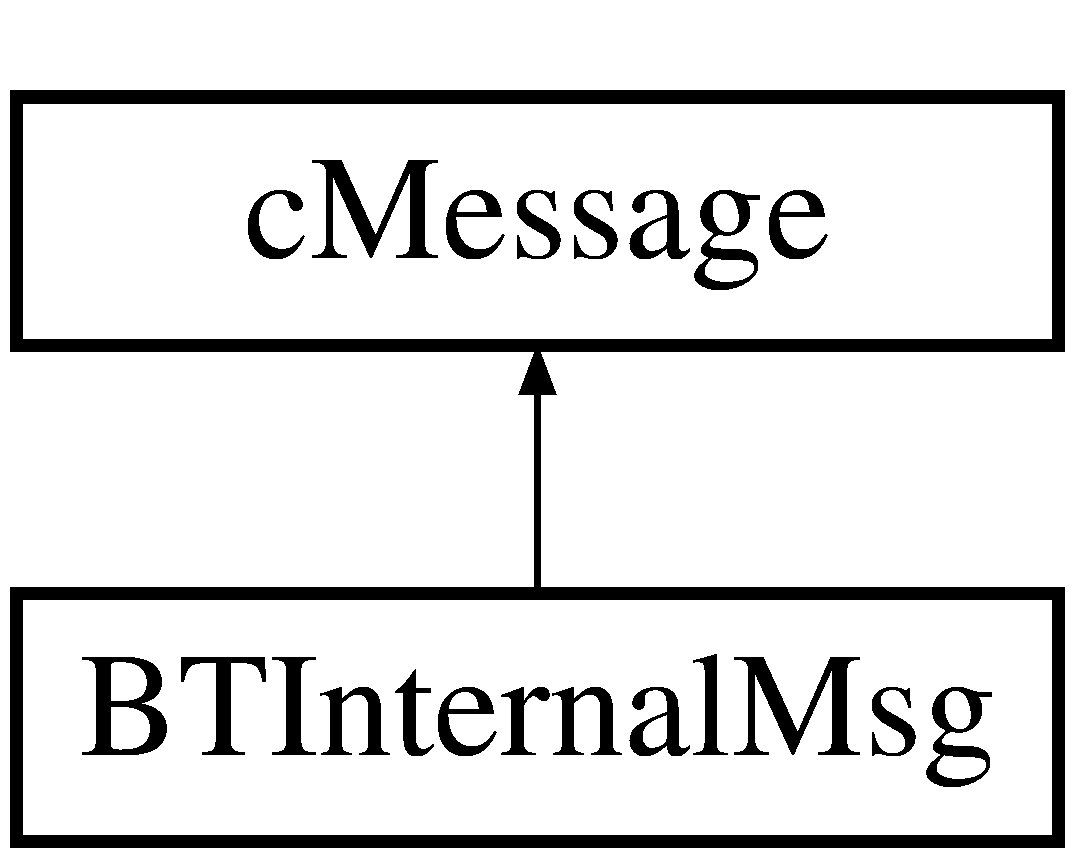
\includegraphics[height=2.000000cm]{classBTInternalMsg}
\end{center}
\end{figure}
\subsection*{Public Member Functions}
\begin{DoxyCompactItemize}
\item 
\hyperlink{classBTInternalMsg_a53b2c681b85235a280f2457f9fd5635c}{B\+T\+Internal\+Msg} (const char $\ast$name=N\+U\+L\+L, int kind=0)
\item 
\hyperlink{classBTInternalMsg_a357a57a913f8e9bbde6e0ec3bf8b2916}{B\+T\+Internal\+Msg} (const \hyperlink{classBTInternalMsg}{B\+T\+Internal\+Msg} \&other)
\item 
virtual \hyperlink{classBTInternalMsg_afe98460fb9ac940a12be1575463db062}{$\sim$\+B\+T\+Internal\+Msg} ()
\item 
\hyperlink{classBTInternalMsg}{B\+T\+Internal\+Msg} \& \hyperlink{classBTInternalMsg_a51f11cbf48627a72aae6f10af630755c}{operator=} (const \hyperlink{classBTInternalMsg}{B\+T\+Internal\+Msg} \&other)
\item 
virtual \hyperlink{classBTInternalMsg}{B\+T\+Internal\+Msg} $\ast$ \hyperlink{classBTInternalMsg_ae50271eba13f59591144f7376b759f47}{dup} () const 
\item 
virtual void \hyperlink{classBTInternalMsg_ab3a268d92a96f2ebacca8a8ddc573c2b}{parsim\+Pack} (c\+Comm\+Buffer $\ast$b)
\item 
virtual void \hyperlink{classBTInternalMsg_ad036d69ceeb72e7745fed2dfe9a2e311}{parsim\+Unpack} (c\+Comm\+Buffer $\ast$b)
\item 
virtual const char $\ast$ \hyperlink{classBTInternalMsg_a2e545dd7e0abe0b1d03339ad4b43ed26}{text} () const 
\item 
virtual void \hyperlink{classBTInternalMsg_a29a8ee557b699a3c753f75112c3d1dde}{set\+Text} (const char $\ast$\hyperlink{classBTInternalMsg_a8c02d34494805be9a533ffd978c02420}{text\+\_\+var})
\item 
virtual \hyperlink{structPEER}{P\+E\+E\+R} \& \hyperlink{classBTInternalMsg_ac31be4b9cd9bd9a974fe4b65dfad8469}{peer} ()
\item 
virtual const \hyperlink{structPEER}{P\+E\+E\+R} \& \hyperlink{classBTInternalMsg_ab81f702ef1442807b835649b63e0112c}{peer} () const 
\item 
virtual void \hyperlink{classBTInternalMsg_a095bd7691fd267f76303106940e5e5d4}{set\+Peer} (const \hyperlink{structPEER}{P\+E\+E\+R} \&\hyperlink{classBTInternalMsg_aedc6acce926c31ae1d032110de29e871}{peer\+\_\+var})
\item 
virtual int \hyperlink{classBTInternalMsg_a408ca06b66f3f1e4680925e6dee51a1c}{piece\+Index} () const 
\item 
virtual void \hyperlink{classBTInternalMsg_a6c96a1f240dd338dec85988abd54ae25}{set\+Piece\+Index} (int \hyperlink{classBTInternalMsg_a74c9e0793d23162bc836a76b78812d88}{piece\+Index\+\_\+var})
\item 
virtual int \hyperlink{classBTInternalMsg_a7a302c1aa5c2aec0829596105213405d}{block\+Index} () const 
\item 
virtual void \hyperlink{classBTInternalMsg_a6a9cfced7412b37f41b23895bbc05951}{set\+Block\+Index} (int \hyperlink{classBTInternalMsg_a9be734970c7a790c56f41915016518cf}{block\+Index\+\_\+var})
\item 
virtual bool \hyperlink{classBTInternalMsg_a38d6f81246543abd935b5d7699f08d16}{choked\+Piece} () const 
\item 
virtual void \hyperlink{classBTInternalMsg_a139833e3fe32ffb3753b723334e761ae}{set\+Choked\+Piece} (bool \hyperlink{classBTInternalMsg_a364b051cdf4428a35ba41b23ee59f103}{choked\+Piece\+\_\+var})
\end{DoxyCompactItemize}
\subsection*{Protected Member Functions}
\begin{DoxyCompactItemize}
\item 
bool \hyperlink{classBTInternalMsg_a44c349d38925d3441076d28f5465d8f9}{operator==} (const \hyperlink{classBTInternalMsg}{B\+T\+Internal\+Msg} \&)
\end{DoxyCompactItemize}
\subsection*{Protected Attributes}
\begin{DoxyCompactItemize}
\item 
opp\+\_\+string \hyperlink{classBTInternalMsg_a8c02d34494805be9a533ffd978c02420}{text\+\_\+var}
\item 
\+::\hyperlink{structPEER}{P\+E\+E\+R} \hyperlink{classBTInternalMsg_aedc6acce926c31ae1d032110de29e871}{peer\+\_\+var}
\item 
int \hyperlink{classBTInternalMsg_a74c9e0793d23162bc836a76b78812d88}{piece\+Index\+\_\+var}
\item 
int \hyperlink{classBTInternalMsg_a9be734970c7a790c56f41915016518cf}{block\+Index\+\_\+var}
\item 
bool \hyperlink{classBTInternalMsg_a364b051cdf4428a35ba41b23ee59f103}{choked\+Piece\+\_\+var}
\end{DoxyCompactItemize}


\subsection{Detailed Description}
Class generated from {\ttfamily applications/x\+Bit\+Torrent/\+B\+T\+Peer\+Wire\+Msg.\+msg} by opp\+\_\+msgc. 
\begin{DoxyPre}
message \hyperlink{classBTInternalMsg}{BTInternalMsg} extends cMessage
\{
    (true);\end{DoxyPre}



\begin{DoxyPre}    string text;
    \hyperlink{structPEER}{PEER} peer;
    int pieceIndex;
    int blockIndex;
    bool chokedPiece;
\}
\end{DoxyPre}
 

\subsection{Constructor \& Destructor Documentation}
\hypertarget{classBTInternalMsg_a53b2c681b85235a280f2457f9fd5635c}{}\index{B\+T\+Internal\+Msg@{B\+T\+Internal\+Msg}!B\+T\+Internal\+Msg@{B\+T\+Internal\+Msg}}
\index{B\+T\+Internal\+Msg@{B\+T\+Internal\+Msg}!B\+T\+Internal\+Msg@{B\+T\+Internal\+Msg}}
\subsubsection[{B\+T\+Internal\+Msg(const char $\ast$name=\+N\+U\+L\+L, int kind=0)}]{\setlength{\rightskip}{0pt plus 5cm}B\+T\+Internal\+Msg\+::\+B\+T\+Internal\+Msg (
\begin{DoxyParamCaption}
\item[{const char $\ast$}]{name = {\ttfamily NULL}, }
\item[{int}]{kind = {\ttfamily 0}}
\end{DoxyParamCaption}
)}\label{classBTInternalMsg_a53b2c681b85235a280f2457f9fd5635c}
\hypertarget{classBTInternalMsg_a357a57a913f8e9bbde6e0ec3bf8b2916}{}\index{B\+T\+Internal\+Msg@{B\+T\+Internal\+Msg}!B\+T\+Internal\+Msg@{B\+T\+Internal\+Msg}}
\index{B\+T\+Internal\+Msg@{B\+T\+Internal\+Msg}!B\+T\+Internal\+Msg@{B\+T\+Internal\+Msg}}
\subsubsection[{B\+T\+Internal\+Msg(const B\+T\+Internal\+Msg \&other)}]{\setlength{\rightskip}{0pt plus 5cm}B\+T\+Internal\+Msg\+::\+B\+T\+Internal\+Msg (
\begin{DoxyParamCaption}
\item[{const {\bf B\+T\+Internal\+Msg} \&}]{other}
\end{DoxyParamCaption}
)}\label{classBTInternalMsg_a357a57a913f8e9bbde6e0ec3bf8b2916}
\hypertarget{classBTInternalMsg_afe98460fb9ac940a12be1575463db062}{}\index{B\+T\+Internal\+Msg@{B\+T\+Internal\+Msg}!````~B\+T\+Internal\+Msg@{$\sim$\+B\+T\+Internal\+Msg}}
\index{````~B\+T\+Internal\+Msg@{$\sim$\+B\+T\+Internal\+Msg}!B\+T\+Internal\+Msg@{B\+T\+Internal\+Msg}}
\subsubsection[{$\sim$\+B\+T\+Internal\+Msg()}]{\setlength{\rightskip}{0pt plus 5cm}B\+T\+Internal\+Msg\+::$\sim$\+B\+T\+Internal\+Msg (
\begin{DoxyParamCaption}
{}
\end{DoxyParamCaption}
)\hspace{0.3cm}{\ttfamily [virtual]}}\label{classBTInternalMsg_afe98460fb9ac940a12be1575463db062}


\subsection{Member Function Documentation}
\hypertarget{classBTInternalMsg_a7a302c1aa5c2aec0829596105213405d}{}\index{B\+T\+Internal\+Msg@{B\+T\+Internal\+Msg}!block\+Index@{block\+Index}}
\index{block\+Index@{block\+Index}!B\+T\+Internal\+Msg@{B\+T\+Internal\+Msg}}
\subsubsection[{block\+Index() const }]{\setlength{\rightskip}{0pt plus 5cm}int B\+T\+Internal\+Msg\+::block\+Index (
\begin{DoxyParamCaption}
{}
\end{DoxyParamCaption}
) const\hspace{0.3cm}{\ttfamily [virtual]}}\label{classBTInternalMsg_a7a302c1aa5c2aec0829596105213405d}
\hypertarget{classBTInternalMsg_a38d6f81246543abd935b5d7699f08d16}{}\index{B\+T\+Internal\+Msg@{B\+T\+Internal\+Msg}!choked\+Piece@{choked\+Piece}}
\index{choked\+Piece@{choked\+Piece}!B\+T\+Internal\+Msg@{B\+T\+Internal\+Msg}}
\subsubsection[{choked\+Piece() const }]{\setlength{\rightskip}{0pt plus 5cm}bool B\+T\+Internal\+Msg\+::choked\+Piece (
\begin{DoxyParamCaption}
{}
\end{DoxyParamCaption}
) const\hspace{0.3cm}{\ttfamily [virtual]}}\label{classBTInternalMsg_a38d6f81246543abd935b5d7699f08d16}
\hypertarget{classBTInternalMsg_ae50271eba13f59591144f7376b759f47}{}\index{B\+T\+Internal\+Msg@{B\+T\+Internal\+Msg}!dup@{dup}}
\index{dup@{dup}!B\+T\+Internal\+Msg@{B\+T\+Internal\+Msg}}
\subsubsection[{dup() const }]{\setlength{\rightskip}{0pt plus 5cm}virtual {\bf B\+T\+Internal\+Msg}$\ast$ B\+T\+Internal\+Msg\+::dup (
\begin{DoxyParamCaption}
{}
\end{DoxyParamCaption}
) const\hspace{0.3cm}{\ttfamily [inline]}, {\ttfamily [virtual]}}\label{classBTInternalMsg_ae50271eba13f59591144f7376b759f47}
\hypertarget{classBTInternalMsg_a51f11cbf48627a72aae6f10af630755c}{}\index{B\+T\+Internal\+Msg@{B\+T\+Internal\+Msg}!operator=@{operator=}}
\index{operator=@{operator=}!B\+T\+Internal\+Msg@{B\+T\+Internal\+Msg}}
\subsubsection[{operator=(const B\+T\+Internal\+Msg \&other)}]{\setlength{\rightskip}{0pt plus 5cm}{\bf B\+T\+Internal\+Msg} \& B\+T\+Internal\+Msg\+::operator= (
\begin{DoxyParamCaption}
\item[{const {\bf B\+T\+Internal\+Msg} \&}]{other}
\end{DoxyParamCaption}
)}\label{classBTInternalMsg_a51f11cbf48627a72aae6f10af630755c}
\hypertarget{classBTInternalMsg_a44c349d38925d3441076d28f5465d8f9}{}\index{B\+T\+Internal\+Msg@{B\+T\+Internal\+Msg}!operator==@{operator==}}
\index{operator==@{operator==}!B\+T\+Internal\+Msg@{B\+T\+Internal\+Msg}}
\subsubsection[{operator==(const B\+T\+Internal\+Msg \&)}]{\setlength{\rightskip}{0pt plus 5cm}bool B\+T\+Internal\+Msg\+::operator== (
\begin{DoxyParamCaption}
\item[{const {\bf B\+T\+Internal\+Msg} \&}]{}
\end{DoxyParamCaption}
)\hspace{0.3cm}{\ttfamily [protected]}}\label{classBTInternalMsg_a44c349d38925d3441076d28f5465d8f9}
\hypertarget{classBTInternalMsg_ab3a268d92a96f2ebacca8a8ddc573c2b}{}\index{B\+T\+Internal\+Msg@{B\+T\+Internal\+Msg}!parsim\+Pack@{parsim\+Pack}}
\index{parsim\+Pack@{parsim\+Pack}!B\+T\+Internal\+Msg@{B\+T\+Internal\+Msg}}
\subsubsection[{parsim\+Pack(c\+Comm\+Buffer $\ast$b)}]{\setlength{\rightskip}{0pt plus 5cm}void B\+T\+Internal\+Msg\+::parsim\+Pack (
\begin{DoxyParamCaption}
\item[{c\+Comm\+Buffer $\ast$}]{b}
\end{DoxyParamCaption}
)\hspace{0.3cm}{\ttfamily [virtual]}}\label{classBTInternalMsg_ab3a268d92a96f2ebacca8a8ddc573c2b}
\hypertarget{classBTInternalMsg_ad036d69ceeb72e7745fed2dfe9a2e311}{}\index{B\+T\+Internal\+Msg@{B\+T\+Internal\+Msg}!parsim\+Unpack@{parsim\+Unpack}}
\index{parsim\+Unpack@{parsim\+Unpack}!B\+T\+Internal\+Msg@{B\+T\+Internal\+Msg}}
\subsubsection[{parsim\+Unpack(c\+Comm\+Buffer $\ast$b)}]{\setlength{\rightskip}{0pt plus 5cm}void B\+T\+Internal\+Msg\+::parsim\+Unpack (
\begin{DoxyParamCaption}
\item[{c\+Comm\+Buffer $\ast$}]{b}
\end{DoxyParamCaption}
)\hspace{0.3cm}{\ttfamily [virtual]}}\label{classBTInternalMsg_ad036d69ceeb72e7745fed2dfe9a2e311}
\hypertarget{classBTInternalMsg_ac31be4b9cd9bd9a974fe4b65dfad8469}{}\index{B\+T\+Internal\+Msg@{B\+T\+Internal\+Msg}!peer@{peer}}
\index{peer@{peer}!B\+T\+Internal\+Msg@{B\+T\+Internal\+Msg}}
\subsubsection[{peer()}]{\setlength{\rightskip}{0pt plus 5cm}{\bf P\+E\+E\+R} \& B\+T\+Internal\+Msg\+::peer (
\begin{DoxyParamCaption}
{}
\end{DoxyParamCaption}
)\hspace{0.3cm}{\ttfamily [virtual]}}\label{classBTInternalMsg_ac31be4b9cd9bd9a974fe4b65dfad8469}
\hypertarget{classBTInternalMsg_ab81f702ef1442807b835649b63e0112c}{}\index{B\+T\+Internal\+Msg@{B\+T\+Internal\+Msg}!peer@{peer}}
\index{peer@{peer}!B\+T\+Internal\+Msg@{B\+T\+Internal\+Msg}}
\subsubsection[{peer() const }]{\setlength{\rightskip}{0pt plus 5cm}virtual const {\bf P\+E\+E\+R}\& B\+T\+Internal\+Msg\+::peer (
\begin{DoxyParamCaption}
{}
\end{DoxyParamCaption}
) const\hspace{0.3cm}{\ttfamily [inline]}, {\ttfamily [virtual]}}\label{classBTInternalMsg_ab81f702ef1442807b835649b63e0112c}
\hypertarget{classBTInternalMsg_a408ca06b66f3f1e4680925e6dee51a1c}{}\index{B\+T\+Internal\+Msg@{B\+T\+Internal\+Msg}!piece\+Index@{piece\+Index}}
\index{piece\+Index@{piece\+Index}!B\+T\+Internal\+Msg@{B\+T\+Internal\+Msg}}
\subsubsection[{piece\+Index() const }]{\setlength{\rightskip}{0pt plus 5cm}int B\+T\+Internal\+Msg\+::piece\+Index (
\begin{DoxyParamCaption}
{}
\end{DoxyParamCaption}
) const\hspace{0.3cm}{\ttfamily [virtual]}}\label{classBTInternalMsg_a408ca06b66f3f1e4680925e6dee51a1c}
\hypertarget{classBTInternalMsg_a6a9cfced7412b37f41b23895bbc05951}{}\index{B\+T\+Internal\+Msg@{B\+T\+Internal\+Msg}!set\+Block\+Index@{set\+Block\+Index}}
\index{set\+Block\+Index@{set\+Block\+Index}!B\+T\+Internal\+Msg@{B\+T\+Internal\+Msg}}
\subsubsection[{set\+Block\+Index(int block\+Index\+\_\+var)}]{\setlength{\rightskip}{0pt plus 5cm}void B\+T\+Internal\+Msg\+::set\+Block\+Index (
\begin{DoxyParamCaption}
\item[{int}]{block\+Index\+\_\+var}
\end{DoxyParamCaption}
)\hspace{0.3cm}{\ttfamily [virtual]}}\label{classBTInternalMsg_a6a9cfced7412b37f41b23895bbc05951}
\hypertarget{classBTInternalMsg_a139833e3fe32ffb3753b723334e761ae}{}\index{B\+T\+Internal\+Msg@{B\+T\+Internal\+Msg}!set\+Choked\+Piece@{set\+Choked\+Piece}}
\index{set\+Choked\+Piece@{set\+Choked\+Piece}!B\+T\+Internal\+Msg@{B\+T\+Internal\+Msg}}
\subsubsection[{set\+Choked\+Piece(bool choked\+Piece\+\_\+var)}]{\setlength{\rightskip}{0pt plus 5cm}void B\+T\+Internal\+Msg\+::set\+Choked\+Piece (
\begin{DoxyParamCaption}
\item[{bool}]{choked\+Piece\+\_\+var}
\end{DoxyParamCaption}
)\hspace{0.3cm}{\ttfamily [virtual]}}\label{classBTInternalMsg_a139833e3fe32ffb3753b723334e761ae}
\hypertarget{classBTInternalMsg_a095bd7691fd267f76303106940e5e5d4}{}\index{B\+T\+Internal\+Msg@{B\+T\+Internal\+Msg}!set\+Peer@{set\+Peer}}
\index{set\+Peer@{set\+Peer}!B\+T\+Internal\+Msg@{B\+T\+Internal\+Msg}}
\subsubsection[{set\+Peer(const P\+E\+E\+R \&peer\+\_\+var)}]{\setlength{\rightskip}{0pt plus 5cm}void B\+T\+Internal\+Msg\+::set\+Peer (
\begin{DoxyParamCaption}
\item[{const {\bf P\+E\+E\+R} \&}]{peer\+\_\+var}
\end{DoxyParamCaption}
)\hspace{0.3cm}{\ttfamily [virtual]}}\label{classBTInternalMsg_a095bd7691fd267f76303106940e5e5d4}
\hypertarget{classBTInternalMsg_a6c96a1f240dd338dec85988abd54ae25}{}\index{B\+T\+Internal\+Msg@{B\+T\+Internal\+Msg}!set\+Piece\+Index@{set\+Piece\+Index}}
\index{set\+Piece\+Index@{set\+Piece\+Index}!B\+T\+Internal\+Msg@{B\+T\+Internal\+Msg}}
\subsubsection[{set\+Piece\+Index(int piece\+Index\+\_\+var)}]{\setlength{\rightskip}{0pt plus 5cm}void B\+T\+Internal\+Msg\+::set\+Piece\+Index (
\begin{DoxyParamCaption}
\item[{int}]{piece\+Index\+\_\+var}
\end{DoxyParamCaption}
)\hspace{0.3cm}{\ttfamily [virtual]}}\label{classBTInternalMsg_a6c96a1f240dd338dec85988abd54ae25}
\hypertarget{classBTInternalMsg_a29a8ee557b699a3c753f75112c3d1dde}{}\index{B\+T\+Internal\+Msg@{B\+T\+Internal\+Msg}!set\+Text@{set\+Text}}
\index{set\+Text@{set\+Text}!B\+T\+Internal\+Msg@{B\+T\+Internal\+Msg}}
\subsubsection[{set\+Text(const char $\ast$text\+\_\+var)}]{\setlength{\rightskip}{0pt plus 5cm}void B\+T\+Internal\+Msg\+::set\+Text (
\begin{DoxyParamCaption}
\item[{const char $\ast$}]{text\+\_\+var}
\end{DoxyParamCaption}
)\hspace{0.3cm}{\ttfamily [virtual]}}\label{classBTInternalMsg_a29a8ee557b699a3c753f75112c3d1dde}
\hypertarget{classBTInternalMsg_a2e545dd7e0abe0b1d03339ad4b43ed26}{}\index{B\+T\+Internal\+Msg@{B\+T\+Internal\+Msg}!text@{text}}
\index{text@{text}!B\+T\+Internal\+Msg@{B\+T\+Internal\+Msg}}
\subsubsection[{text() const }]{\setlength{\rightskip}{0pt plus 5cm}const char $\ast$ B\+T\+Internal\+Msg\+::text (
\begin{DoxyParamCaption}
{}
\end{DoxyParamCaption}
) const\hspace{0.3cm}{\ttfamily [virtual]}}\label{classBTInternalMsg_a2e545dd7e0abe0b1d03339ad4b43ed26}


\subsection{Member Data Documentation}
\hypertarget{classBTInternalMsg_a9be734970c7a790c56f41915016518cf}{}\index{B\+T\+Internal\+Msg@{B\+T\+Internal\+Msg}!block\+Index\+\_\+var@{block\+Index\+\_\+var}}
\index{block\+Index\+\_\+var@{block\+Index\+\_\+var}!B\+T\+Internal\+Msg@{B\+T\+Internal\+Msg}}
\subsubsection[{block\+Index\+\_\+var}]{\setlength{\rightskip}{0pt plus 5cm}int B\+T\+Internal\+Msg\+::block\+Index\+\_\+var\hspace{0.3cm}{\ttfamily [protected]}}\label{classBTInternalMsg_a9be734970c7a790c56f41915016518cf}
\hypertarget{classBTInternalMsg_a364b051cdf4428a35ba41b23ee59f103}{}\index{B\+T\+Internal\+Msg@{B\+T\+Internal\+Msg}!choked\+Piece\+\_\+var@{choked\+Piece\+\_\+var}}
\index{choked\+Piece\+\_\+var@{choked\+Piece\+\_\+var}!B\+T\+Internal\+Msg@{B\+T\+Internal\+Msg}}
\subsubsection[{choked\+Piece\+\_\+var}]{\setlength{\rightskip}{0pt plus 5cm}bool B\+T\+Internal\+Msg\+::choked\+Piece\+\_\+var\hspace{0.3cm}{\ttfamily [protected]}}\label{classBTInternalMsg_a364b051cdf4428a35ba41b23ee59f103}
\hypertarget{classBTInternalMsg_aedc6acce926c31ae1d032110de29e871}{}\index{B\+T\+Internal\+Msg@{B\+T\+Internal\+Msg}!peer\+\_\+var@{peer\+\_\+var}}
\index{peer\+\_\+var@{peer\+\_\+var}!B\+T\+Internal\+Msg@{B\+T\+Internal\+Msg}}
\subsubsection[{peer\+\_\+var}]{\setlength{\rightskip}{0pt plus 5cm}\+::{\bf P\+E\+E\+R} B\+T\+Internal\+Msg\+::peer\+\_\+var\hspace{0.3cm}{\ttfamily [protected]}}\label{classBTInternalMsg_aedc6acce926c31ae1d032110de29e871}
\hypertarget{classBTInternalMsg_a74c9e0793d23162bc836a76b78812d88}{}\index{B\+T\+Internal\+Msg@{B\+T\+Internal\+Msg}!piece\+Index\+\_\+var@{piece\+Index\+\_\+var}}
\index{piece\+Index\+\_\+var@{piece\+Index\+\_\+var}!B\+T\+Internal\+Msg@{B\+T\+Internal\+Msg}}
\subsubsection[{piece\+Index\+\_\+var}]{\setlength{\rightskip}{0pt plus 5cm}int B\+T\+Internal\+Msg\+::piece\+Index\+\_\+var\hspace{0.3cm}{\ttfamily [protected]}}\label{classBTInternalMsg_a74c9e0793d23162bc836a76b78812d88}
\hypertarget{classBTInternalMsg_a8c02d34494805be9a533ffd978c02420}{}\index{B\+T\+Internal\+Msg@{B\+T\+Internal\+Msg}!text\+\_\+var@{text\+\_\+var}}
\index{text\+\_\+var@{text\+\_\+var}!B\+T\+Internal\+Msg@{B\+T\+Internal\+Msg}}
\subsubsection[{text\+\_\+var}]{\setlength{\rightskip}{0pt plus 5cm}opp\+\_\+string B\+T\+Internal\+Msg\+::text\+\_\+var\hspace{0.3cm}{\ttfamily [protected]}}\label{classBTInternalMsg_a8c02d34494805be9a533ffd978c02420}


The documentation for this class was generated from the following files\+:\begin{DoxyCompactItemize}
\item 
\hyperlink{BTPeerWireMsg__m_8h}{B\+T\+Peer\+Wire\+Msg\+\_\+m.\+h}\item 
\hyperlink{BTPeerWireMsg__m_8cc}{B\+T\+Peer\+Wire\+Msg\+\_\+m.\+cc}\end{DoxyCompactItemize}

\hypertarget{classBTInternalMsgDescriptor}{}\section{B\+T\+Internal\+Msg\+Descriptor Class Reference}
\label{classBTInternalMsgDescriptor}\index{B\+T\+Internal\+Msg\+Descriptor@{B\+T\+Internal\+Msg\+Descriptor}}
Inheritance diagram for B\+T\+Internal\+Msg\+Descriptor\+:\begin{figure}[H]
\begin{center}
\leavevmode
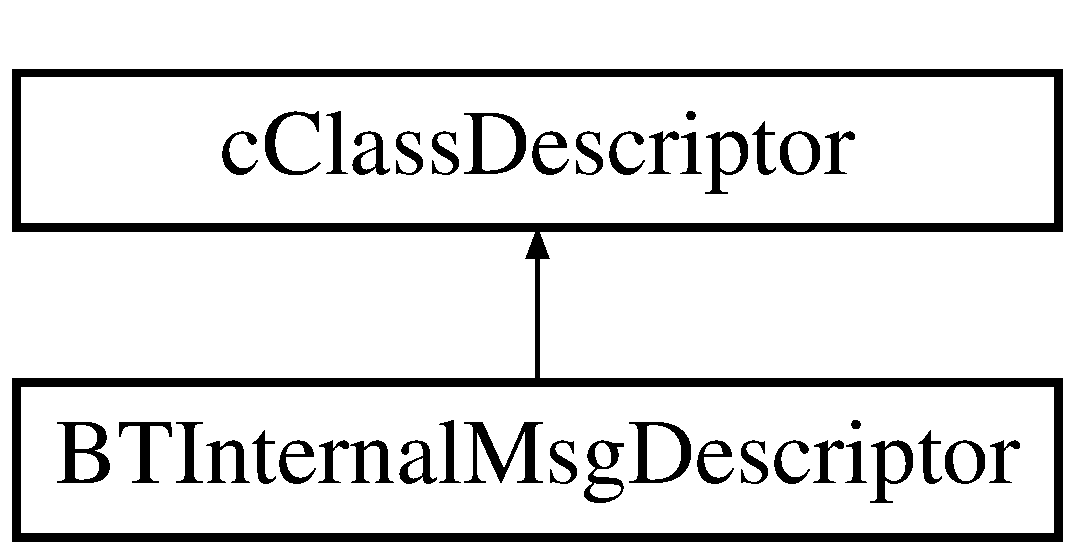
\includegraphics[height=2.000000cm]{classBTInternalMsgDescriptor}
\end{center}
\end{figure}
\subsection*{Public Member Functions}
\begin{DoxyCompactItemize}
\item 
\hyperlink{classBTInternalMsgDescriptor_ab80f6626bd7e6c9ed08f56b7524431b7}{B\+T\+Internal\+Msg\+Descriptor} ()
\item 
virtual \hyperlink{classBTInternalMsgDescriptor_ada07c2205448521107d60449ecccbeba}{$\sim$\+B\+T\+Internal\+Msg\+Descriptor} ()
\item 
virtual bool \hyperlink{classBTInternalMsgDescriptor_acdff02ce9abff61fe3d32c7857e71433}{does\+Support} (c\+Object $\ast$obj) const 
\item 
virtual const char $\ast$ \hyperlink{classBTInternalMsgDescriptor_a46ecca01196b00552c7b992ef015195a}{get\+Property} (const char $\ast$propertyname) const 
\item 
virtual int \hyperlink{classBTInternalMsgDescriptor_a34e1041cfd1bab108cbaa1ffa398d9a1}{get\+Field\+Count} (void $\ast$object) const 
\item 
virtual const char $\ast$ \hyperlink{classBTInternalMsgDescriptor_a7e95cc140d1826c13447b655ca07d468}{get\+Field\+Name} (void $\ast$object, int field) const 
\item 
virtual int \hyperlink{classBTInternalMsgDescriptor_a10949d2641e4383e115fb337ecb29c2a}{find\+Field} (void $\ast$object, const char $\ast$field\+Name) const 
\item 
virtual unsigned int \hyperlink{classBTInternalMsgDescriptor_ad6248569e6541cd769eb4e24d8e84b51}{get\+Field\+Type\+Flags} (void $\ast$object, int field) const 
\item 
virtual const char $\ast$ \hyperlink{classBTInternalMsgDescriptor_a3db0bb17f4f3223e7f676b17e317cc47}{get\+Field\+Type\+String} (void $\ast$object, int field) const 
\item 
virtual const char $\ast$ \hyperlink{classBTInternalMsgDescriptor_a3f6a81e5d8dd6d0ad4c3ecb86e59c42f}{get\+Field\+Property} (void $\ast$object, int field, const char $\ast$propertyname) const 
\item 
virtual int \hyperlink{classBTInternalMsgDescriptor_a2e8260c9d02eceda6c1590f4d552a638}{get\+Array\+Size} (void $\ast$object, int field) const 
\item 
virtual std\+::string \hyperlink{classBTInternalMsgDescriptor_ab8b9906a3147322ab4c0d33556db47ad}{get\+Field\+As\+String} (void $\ast$object, int field, int i) const 
\item 
virtual bool \hyperlink{classBTInternalMsgDescriptor_afaa61cb44223a4144626776093f436a8}{set\+Field\+As\+String} (void $\ast$object, int field, int i, const char $\ast$value) const 
\item 
virtual const char $\ast$ \hyperlink{classBTInternalMsgDescriptor_a634938d55229e78937cd07fcafddcf2b}{get\+Field\+Struct\+Name} (void $\ast$object, int field) const 
\item 
virtual void $\ast$ \hyperlink{classBTInternalMsgDescriptor_ab1d46a660013e3de5ad3c928cb2c801c}{get\+Field\+Struct\+Pointer} (void $\ast$object, int field, int i) const 
\end{DoxyCompactItemize}


\subsection{Constructor \& Destructor Documentation}
\hypertarget{classBTInternalMsgDescriptor_ab80f6626bd7e6c9ed08f56b7524431b7}{}\index{B\+T\+Internal\+Msg\+Descriptor@{B\+T\+Internal\+Msg\+Descriptor}!B\+T\+Internal\+Msg\+Descriptor@{B\+T\+Internal\+Msg\+Descriptor}}
\index{B\+T\+Internal\+Msg\+Descriptor@{B\+T\+Internal\+Msg\+Descriptor}!B\+T\+Internal\+Msg\+Descriptor@{B\+T\+Internal\+Msg\+Descriptor}}
\subsubsection[{B\+T\+Internal\+Msg\+Descriptor()}]{\setlength{\rightskip}{0pt plus 5cm}B\+T\+Internal\+Msg\+Descriptor\+::\+B\+T\+Internal\+Msg\+Descriptor (
\begin{DoxyParamCaption}
{}
\end{DoxyParamCaption}
)}\label{classBTInternalMsgDescriptor_ab80f6626bd7e6c9ed08f56b7524431b7}
\hypertarget{classBTInternalMsgDescriptor_ada07c2205448521107d60449ecccbeba}{}\index{B\+T\+Internal\+Msg\+Descriptor@{B\+T\+Internal\+Msg\+Descriptor}!````~B\+T\+Internal\+Msg\+Descriptor@{$\sim$\+B\+T\+Internal\+Msg\+Descriptor}}
\index{````~B\+T\+Internal\+Msg\+Descriptor@{$\sim$\+B\+T\+Internal\+Msg\+Descriptor}!B\+T\+Internal\+Msg\+Descriptor@{B\+T\+Internal\+Msg\+Descriptor}}
\subsubsection[{$\sim$\+B\+T\+Internal\+Msg\+Descriptor()}]{\setlength{\rightskip}{0pt plus 5cm}B\+T\+Internal\+Msg\+Descriptor\+::$\sim$\+B\+T\+Internal\+Msg\+Descriptor (
\begin{DoxyParamCaption}
{}
\end{DoxyParamCaption}
)\hspace{0.3cm}{\ttfamily [virtual]}}\label{classBTInternalMsgDescriptor_ada07c2205448521107d60449ecccbeba}


\subsection{Member Function Documentation}
\hypertarget{classBTInternalMsgDescriptor_acdff02ce9abff61fe3d32c7857e71433}{}\index{B\+T\+Internal\+Msg\+Descriptor@{B\+T\+Internal\+Msg\+Descriptor}!does\+Support@{does\+Support}}
\index{does\+Support@{does\+Support}!B\+T\+Internal\+Msg\+Descriptor@{B\+T\+Internal\+Msg\+Descriptor}}
\subsubsection[{does\+Support(c\+Object $\ast$obj) const }]{\setlength{\rightskip}{0pt plus 5cm}bool B\+T\+Internal\+Msg\+Descriptor\+::does\+Support (
\begin{DoxyParamCaption}
\item[{c\+Object $\ast$}]{obj}
\end{DoxyParamCaption}
) const\hspace{0.3cm}{\ttfamily [virtual]}}\label{classBTInternalMsgDescriptor_acdff02ce9abff61fe3d32c7857e71433}
\hypertarget{classBTInternalMsgDescriptor_a10949d2641e4383e115fb337ecb29c2a}{}\index{B\+T\+Internal\+Msg\+Descriptor@{B\+T\+Internal\+Msg\+Descriptor}!find\+Field@{find\+Field}}
\index{find\+Field@{find\+Field}!B\+T\+Internal\+Msg\+Descriptor@{B\+T\+Internal\+Msg\+Descriptor}}
\subsubsection[{find\+Field(void $\ast$object, const char $\ast$field\+Name) const }]{\setlength{\rightskip}{0pt plus 5cm}int B\+T\+Internal\+Msg\+Descriptor\+::find\+Field (
\begin{DoxyParamCaption}
\item[{void $\ast$}]{object, }
\item[{const char $\ast$}]{field\+Name}
\end{DoxyParamCaption}
) const\hspace{0.3cm}{\ttfamily [virtual]}}\label{classBTInternalMsgDescriptor_a10949d2641e4383e115fb337ecb29c2a}
\hypertarget{classBTInternalMsgDescriptor_a2e8260c9d02eceda6c1590f4d552a638}{}\index{B\+T\+Internal\+Msg\+Descriptor@{B\+T\+Internal\+Msg\+Descriptor}!get\+Array\+Size@{get\+Array\+Size}}
\index{get\+Array\+Size@{get\+Array\+Size}!B\+T\+Internal\+Msg\+Descriptor@{B\+T\+Internal\+Msg\+Descriptor}}
\subsubsection[{get\+Array\+Size(void $\ast$object, int field) const }]{\setlength{\rightskip}{0pt plus 5cm}int B\+T\+Internal\+Msg\+Descriptor\+::get\+Array\+Size (
\begin{DoxyParamCaption}
\item[{void $\ast$}]{object, }
\item[{int}]{field}
\end{DoxyParamCaption}
) const\hspace{0.3cm}{\ttfamily [virtual]}}\label{classBTInternalMsgDescriptor_a2e8260c9d02eceda6c1590f4d552a638}
\hypertarget{classBTInternalMsgDescriptor_ab8b9906a3147322ab4c0d33556db47ad}{}\index{B\+T\+Internal\+Msg\+Descriptor@{B\+T\+Internal\+Msg\+Descriptor}!get\+Field\+As\+String@{get\+Field\+As\+String}}
\index{get\+Field\+As\+String@{get\+Field\+As\+String}!B\+T\+Internal\+Msg\+Descriptor@{B\+T\+Internal\+Msg\+Descriptor}}
\subsubsection[{get\+Field\+As\+String(void $\ast$object, int field, int i) const }]{\setlength{\rightskip}{0pt plus 5cm}std\+::string B\+T\+Internal\+Msg\+Descriptor\+::get\+Field\+As\+String (
\begin{DoxyParamCaption}
\item[{void $\ast$}]{object, }
\item[{int}]{field, }
\item[{int}]{i}
\end{DoxyParamCaption}
) const\hspace{0.3cm}{\ttfamily [virtual]}}\label{classBTInternalMsgDescriptor_ab8b9906a3147322ab4c0d33556db47ad}
\hypertarget{classBTInternalMsgDescriptor_a34e1041cfd1bab108cbaa1ffa398d9a1}{}\index{B\+T\+Internal\+Msg\+Descriptor@{B\+T\+Internal\+Msg\+Descriptor}!get\+Field\+Count@{get\+Field\+Count}}
\index{get\+Field\+Count@{get\+Field\+Count}!B\+T\+Internal\+Msg\+Descriptor@{B\+T\+Internal\+Msg\+Descriptor}}
\subsubsection[{get\+Field\+Count(void $\ast$object) const }]{\setlength{\rightskip}{0pt plus 5cm}int B\+T\+Internal\+Msg\+Descriptor\+::get\+Field\+Count (
\begin{DoxyParamCaption}
\item[{void $\ast$}]{object}
\end{DoxyParamCaption}
) const\hspace{0.3cm}{\ttfamily [virtual]}}\label{classBTInternalMsgDescriptor_a34e1041cfd1bab108cbaa1ffa398d9a1}
\hypertarget{classBTInternalMsgDescriptor_a7e95cc140d1826c13447b655ca07d468}{}\index{B\+T\+Internal\+Msg\+Descriptor@{B\+T\+Internal\+Msg\+Descriptor}!get\+Field\+Name@{get\+Field\+Name}}
\index{get\+Field\+Name@{get\+Field\+Name}!B\+T\+Internal\+Msg\+Descriptor@{B\+T\+Internal\+Msg\+Descriptor}}
\subsubsection[{get\+Field\+Name(void $\ast$object, int field) const }]{\setlength{\rightskip}{0pt plus 5cm}const char $\ast$ B\+T\+Internal\+Msg\+Descriptor\+::get\+Field\+Name (
\begin{DoxyParamCaption}
\item[{void $\ast$}]{object, }
\item[{int}]{field}
\end{DoxyParamCaption}
) const\hspace{0.3cm}{\ttfamily [virtual]}}\label{classBTInternalMsgDescriptor_a7e95cc140d1826c13447b655ca07d468}
\hypertarget{classBTInternalMsgDescriptor_a3f6a81e5d8dd6d0ad4c3ecb86e59c42f}{}\index{B\+T\+Internal\+Msg\+Descriptor@{B\+T\+Internal\+Msg\+Descriptor}!get\+Field\+Property@{get\+Field\+Property}}
\index{get\+Field\+Property@{get\+Field\+Property}!B\+T\+Internal\+Msg\+Descriptor@{B\+T\+Internal\+Msg\+Descriptor}}
\subsubsection[{get\+Field\+Property(void $\ast$object, int field, const char $\ast$propertyname) const }]{\setlength{\rightskip}{0pt plus 5cm}const char $\ast$ B\+T\+Internal\+Msg\+Descriptor\+::get\+Field\+Property (
\begin{DoxyParamCaption}
\item[{void $\ast$}]{object, }
\item[{int}]{field, }
\item[{const char $\ast$}]{propertyname}
\end{DoxyParamCaption}
) const\hspace{0.3cm}{\ttfamily [virtual]}}\label{classBTInternalMsgDescriptor_a3f6a81e5d8dd6d0ad4c3ecb86e59c42f}
\hypertarget{classBTInternalMsgDescriptor_a634938d55229e78937cd07fcafddcf2b}{}\index{B\+T\+Internal\+Msg\+Descriptor@{B\+T\+Internal\+Msg\+Descriptor}!get\+Field\+Struct\+Name@{get\+Field\+Struct\+Name}}
\index{get\+Field\+Struct\+Name@{get\+Field\+Struct\+Name}!B\+T\+Internal\+Msg\+Descriptor@{B\+T\+Internal\+Msg\+Descriptor}}
\subsubsection[{get\+Field\+Struct\+Name(void $\ast$object, int field) const }]{\setlength{\rightskip}{0pt plus 5cm}const char $\ast$ B\+T\+Internal\+Msg\+Descriptor\+::get\+Field\+Struct\+Name (
\begin{DoxyParamCaption}
\item[{void $\ast$}]{object, }
\item[{int}]{field}
\end{DoxyParamCaption}
) const\hspace{0.3cm}{\ttfamily [virtual]}}\label{classBTInternalMsgDescriptor_a634938d55229e78937cd07fcafddcf2b}
\hypertarget{classBTInternalMsgDescriptor_ab1d46a660013e3de5ad3c928cb2c801c}{}\index{B\+T\+Internal\+Msg\+Descriptor@{B\+T\+Internal\+Msg\+Descriptor}!get\+Field\+Struct\+Pointer@{get\+Field\+Struct\+Pointer}}
\index{get\+Field\+Struct\+Pointer@{get\+Field\+Struct\+Pointer}!B\+T\+Internal\+Msg\+Descriptor@{B\+T\+Internal\+Msg\+Descriptor}}
\subsubsection[{get\+Field\+Struct\+Pointer(void $\ast$object, int field, int i) const }]{\setlength{\rightskip}{0pt plus 5cm}void $\ast$ B\+T\+Internal\+Msg\+Descriptor\+::get\+Field\+Struct\+Pointer (
\begin{DoxyParamCaption}
\item[{void $\ast$}]{object, }
\item[{int}]{field, }
\item[{int}]{i}
\end{DoxyParamCaption}
) const\hspace{0.3cm}{\ttfamily [virtual]}}\label{classBTInternalMsgDescriptor_ab1d46a660013e3de5ad3c928cb2c801c}
\hypertarget{classBTInternalMsgDescriptor_ad6248569e6541cd769eb4e24d8e84b51}{}\index{B\+T\+Internal\+Msg\+Descriptor@{B\+T\+Internal\+Msg\+Descriptor}!get\+Field\+Type\+Flags@{get\+Field\+Type\+Flags}}
\index{get\+Field\+Type\+Flags@{get\+Field\+Type\+Flags}!B\+T\+Internal\+Msg\+Descriptor@{B\+T\+Internal\+Msg\+Descriptor}}
\subsubsection[{get\+Field\+Type\+Flags(void $\ast$object, int field) const }]{\setlength{\rightskip}{0pt plus 5cm}unsigned int B\+T\+Internal\+Msg\+Descriptor\+::get\+Field\+Type\+Flags (
\begin{DoxyParamCaption}
\item[{void $\ast$}]{object, }
\item[{int}]{field}
\end{DoxyParamCaption}
) const\hspace{0.3cm}{\ttfamily [virtual]}}\label{classBTInternalMsgDescriptor_ad6248569e6541cd769eb4e24d8e84b51}
\hypertarget{classBTInternalMsgDescriptor_a3db0bb17f4f3223e7f676b17e317cc47}{}\index{B\+T\+Internal\+Msg\+Descriptor@{B\+T\+Internal\+Msg\+Descriptor}!get\+Field\+Type\+String@{get\+Field\+Type\+String}}
\index{get\+Field\+Type\+String@{get\+Field\+Type\+String}!B\+T\+Internal\+Msg\+Descriptor@{B\+T\+Internal\+Msg\+Descriptor}}
\subsubsection[{get\+Field\+Type\+String(void $\ast$object, int field) const }]{\setlength{\rightskip}{0pt plus 5cm}const char $\ast$ B\+T\+Internal\+Msg\+Descriptor\+::get\+Field\+Type\+String (
\begin{DoxyParamCaption}
\item[{void $\ast$}]{object, }
\item[{int}]{field}
\end{DoxyParamCaption}
) const\hspace{0.3cm}{\ttfamily [virtual]}}\label{classBTInternalMsgDescriptor_a3db0bb17f4f3223e7f676b17e317cc47}
\hypertarget{classBTInternalMsgDescriptor_a46ecca01196b00552c7b992ef015195a}{}\index{B\+T\+Internal\+Msg\+Descriptor@{B\+T\+Internal\+Msg\+Descriptor}!get\+Property@{get\+Property}}
\index{get\+Property@{get\+Property}!B\+T\+Internal\+Msg\+Descriptor@{B\+T\+Internal\+Msg\+Descriptor}}
\subsubsection[{get\+Property(const char $\ast$propertyname) const }]{\setlength{\rightskip}{0pt plus 5cm}const char $\ast$ B\+T\+Internal\+Msg\+Descriptor\+::get\+Property (
\begin{DoxyParamCaption}
\item[{const char $\ast$}]{propertyname}
\end{DoxyParamCaption}
) const\hspace{0.3cm}{\ttfamily [virtual]}}\label{classBTInternalMsgDescriptor_a46ecca01196b00552c7b992ef015195a}
\hypertarget{classBTInternalMsgDescriptor_afaa61cb44223a4144626776093f436a8}{}\index{B\+T\+Internal\+Msg\+Descriptor@{B\+T\+Internal\+Msg\+Descriptor}!set\+Field\+As\+String@{set\+Field\+As\+String}}
\index{set\+Field\+As\+String@{set\+Field\+As\+String}!B\+T\+Internal\+Msg\+Descriptor@{B\+T\+Internal\+Msg\+Descriptor}}
\subsubsection[{set\+Field\+As\+String(void $\ast$object, int field, int i, const char $\ast$value) const }]{\setlength{\rightskip}{0pt plus 5cm}bool B\+T\+Internal\+Msg\+Descriptor\+::set\+Field\+As\+String (
\begin{DoxyParamCaption}
\item[{void $\ast$}]{object, }
\item[{int}]{field, }
\item[{int}]{i, }
\item[{const char $\ast$}]{value}
\end{DoxyParamCaption}
) const\hspace{0.3cm}{\ttfamily [virtual]}}\label{classBTInternalMsgDescriptor_afaa61cb44223a4144626776093f436a8}


The documentation for this class was generated from the following file\+:\begin{DoxyCompactItemize}
\item 
\hyperlink{BTPeerWireMsg__m_8cc}{B\+T\+Peer\+Wire\+Msg\+\_\+m.\+cc}\end{DoxyCompactItemize}

\hypertarget{classBTKeepAliveMsg}{}\section{B\+T\+Keep\+Alive\+Msg Class Reference}
\label{classBTKeepAliveMsg}\index{B\+T\+Keep\+Alive\+Msg@{B\+T\+Keep\+Alive\+Msg}}


{\ttfamily \#include $<$B\+T\+Peer\+Wire\+Msg\+\_\+m.\+h$>$}

Inheritance diagram for B\+T\+Keep\+Alive\+Msg\+:\begin{figure}[H]
\begin{center}
\leavevmode
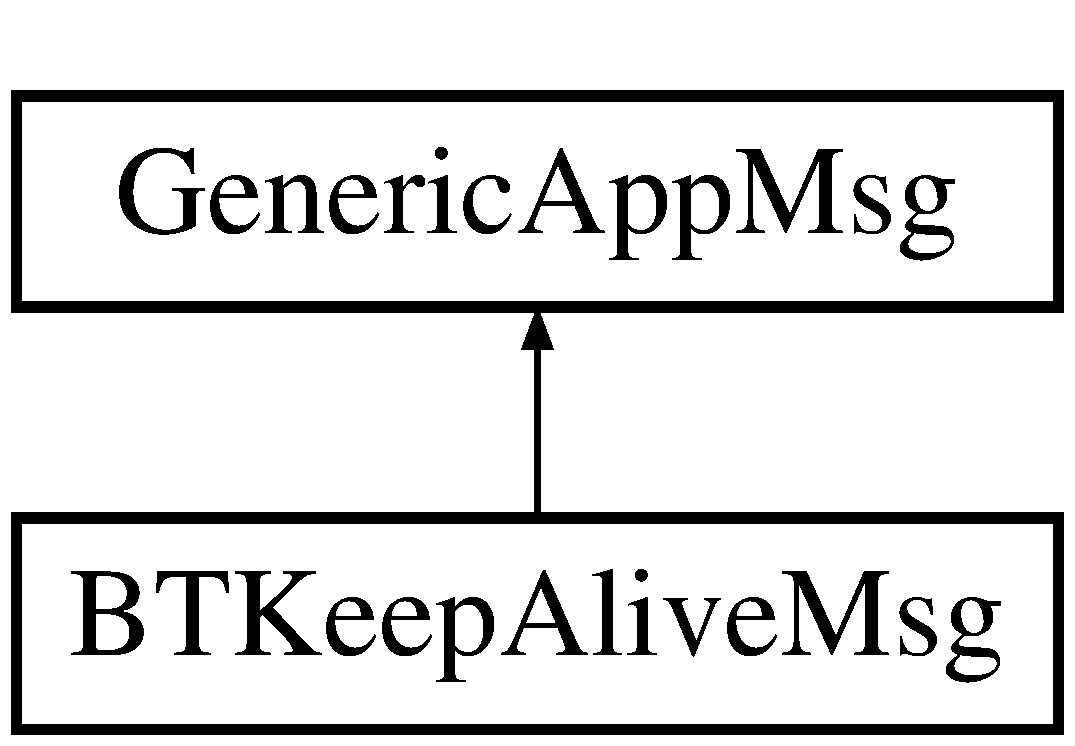
\includegraphics[height=2.000000cm]{classBTKeepAliveMsg}
\end{center}
\end{figure}
\subsection*{Public Member Functions}
\begin{DoxyCompactItemize}
\item 
\hyperlink{classBTKeepAliveMsg_a7d9a58900831a1ba095dfbde7d7be33a}{B\+T\+Keep\+Alive\+Msg} (const char $\ast$name=N\+U\+L\+L, int kind=0)
\item 
\hyperlink{classBTKeepAliveMsg_a9ce38e0df3601cd71f4d2f51ff2bd09d}{B\+T\+Keep\+Alive\+Msg} (const \hyperlink{classBTKeepAliveMsg}{B\+T\+Keep\+Alive\+Msg} \&other)
\item 
virtual \hyperlink{classBTKeepAliveMsg_a6c23e4aac5102beca1de9988a145c0e8}{$\sim$\+B\+T\+Keep\+Alive\+Msg} ()
\item 
\hyperlink{classBTKeepAliveMsg}{B\+T\+Keep\+Alive\+Msg} \& \hyperlink{classBTKeepAliveMsg_a7c915b5dcf9eb4f6dbc13b54aaba54c3}{operator=} (const \hyperlink{classBTKeepAliveMsg}{B\+T\+Keep\+Alive\+Msg} \&other)
\item 
virtual \hyperlink{classBTKeepAliveMsg}{B\+T\+Keep\+Alive\+Msg} $\ast$ \hyperlink{classBTKeepAliveMsg_a78c1a768c8a1724a3920c38825fd76f2}{dup} () const 
\item 
virtual void \hyperlink{classBTKeepAliveMsg_ad7fca4e57bb7bc2e0f52714b1ab59497}{parsim\+Pack} (c\+Comm\+Buffer $\ast$b)
\item 
virtual void \hyperlink{classBTKeepAliveMsg_abc3e9c12e7bd5031abf370577b23ee84}{parsim\+Unpack} (c\+Comm\+Buffer $\ast$b)
\item 
virtual int \hyperlink{classBTKeepAliveMsg_a2f9bca506f768fd7a15e6e0d8692c540}{length\+\_\+prefix} () const 
\item 
virtual void \hyperlink{classBTKeepAliveMsg_a491c41f40ffc11c132e48393fe2c5c52}{set\+Length\+\_\+prefix} (int \hyperlink{classBTKeepAliveMsg_a966d742d7272d0ae62f7954fa2607644}{length\+\_\+prefix\+\_\+var})
\end{DoxyCompactItemize}
\subsection*{Protected Member Functions}
\begin{DoxyCompactItemize}
\item 
bool \hyperlink{classBTKeepAliveMsg_a472011fff095254246151f1abbc919d9}{operator==} (const \hyperlink{classBTKeepAliveMsg}{B\+T\+Keep\+Alive\+Msg} \&)
\end{DoxyCompactItemize}
\subsection*{Protected Attributes}
\begin{DoxyCompactItemize}
\item 
int \hyperlink{classBTKeepAliveMsg_a966d742d7272d0ae62f7954fa2607644}{length\+\_\+prefix\+\_\+var}
\end{DoxyCompactItemize}


\subsection{Detailed Description}
Class generated from {\ttfamily applications/x\+Bit\+Torrent/\+B\+T\+Peer\+Wire\+Msg.\+msg} by opp\+\_\+msgc. 
\begin{DoxyPre}
message \hyperlink{classBTKeepAliveMsg}{BTKeepAliveMsg} extends GenericAppMsg
\{
    (true);\end{DoxyPre}



\begin{DoxyPre}    int length\_prefix;
\}
\end{DoxyPre}
 

\subsection{Constructor \& Destructor Documentation}
\hypertarget{classBTKeepAliveMsg_a7d9a58900831a1ba095dfbde7d7be33a}{}\index{B\+T\+Keep\+Alive\+Msg@{B\+T\+Keep\+Alive\+Msg}!B\+T\+Keep\+Alive\+Msg@{B\+T\+Keep\+Alive\+Msg}}
\index{B\+T\+Keep\+Alive\+Msg@{B\+T\+Keep\+Alive\+Msg}!B\+T\+Keep\+Alive\+Msg@{B\+T\+Keep\+Alive\+Msg}}
\subsubsection[{B\+T\+Keep\+Alive\+Msg(const char $\ast$name=\+N\+U\+L\+L, int kind=0)}]{\setlength{\rightskip}{0pt plus 5cm}B\+T\+Keep\+Alive\+Msg\+::\+B\+T\+Keep\+Alive\+Msg (
\begin{DoxyParamCaption}
\item[{const char $\ast$}]{name = {\ttfamily NULL}, }
\item[{int}]{kind = {\ttfamily 0}}
\end{DoxyParamCaption}
)}\label{classBTKeepAliveMsg_a7d9a58900831a1ba095dfbde7d7be33a}
\hypertarget{classBTKeepAliveMsg_a9ce38e0df3601cd71f4d2f51ff2bd09d}{}\index{B\+T\+Keep\+Alive\+Msg@{B\+T\+Keep\+Alive\+Msg}!B\+T\+Keep\+Alive\+Msg@{B\+T\+Keep\+Alive\+Msg}}
\index{B\+T\+Keep\+Alive\+Msg@{B\+T\+Keep\+Alive\+Msg}!B\+T\+Keep\+Alive\+Msg@{B\+T\+Keep\+Alive\+Msg}}
\subsubsection[{B\+T\+Keep\+Alive\+Msg(const B\+T\+Keep\+Alive\+Msg \&other)}]{\setlength{\rightskip}{0pt plus 5cm}B\+T\+Keep\+Alive\+Msg\+::\+B\+T\+Keep\+Alive\+Msg (
\begin{DoxyParamCaption}
\item[{const {\bf B\+T\+Keep\+Alive\+Msg} \&}]{other}
\end{DoxyParamCaption}
)}\label{classBTKeepAliveMsg_a9ce38e0df3601cd71f4d2f51ff2bd09d}
\hypertarget{classBTKeepAliveMsg_a6c23e4aac5102beca1de9988a145c0e8}{}\index{B\+T\+Keep\+Alive\+Msg@{B\+T\+Keep\+Alive\+Msg}!````~B\+T\+Keep\+Alive\+Msg@{$\sim$\+B\+T\+Keep\+Alive\+Msg}}
\index{````~B\+T\+Keep\+Alive\+Msg@{$\sim$\+B\+T\+Keep\+Alive\+Msg}!B\+T\+Keep\+Alive\+Msg@{B\+T\+Keep\+Alive\+Msg}}
\subsubsection[{$\sim$\+B\+T\+Keep\+Alive\+Msg()}]{\setlength{\rightskip}{0pt plus 5cm}B\+T\+Keep\+Alive\+Msg\+::$\sim$\+B\+T\+Keep\+Alive\+Msg (
\begin{DoxyParamCaption}
{}
\end{DoxyParamCaption}
)\hspace{0.3cm}{\ttfamily [virtual]}}\label{classBTKeepAliveMsg_a6c23e4aac5102beca1de9988a145c0e8}


\subsection{Member Function Documentation}
\hypertarget{classBTKeepAliveMsg_a78c1a768c8a1724a3920c38825fd76f2}{}\index{B\+T\+Keep\+Alive\+Msg@{B\+T\+Keep\+Alive\+Msg}!dup@{dup}}
\index{dup@{dup}!B\+T\+Keep\+Alive\+Msg@{B\+T\+Keep\+Alive\+Msg}}
\subsubsection[{dup() const }]{\setlength{\rightskip}{0pt plus 5cm}virtual {\bf B\+T\+Keep\+Alive\+Msg}$\ast$ B\+T\+Keep\+Alive\+Msg\+::dup (
\begin{DoxyParamCaption}
{}
\end{DoxyParamCaption}
) const\hspace{0.3cm}{\ttfamily [inline]}, {\ttfamily [virtual]}}\label{classBTKeepAliveMsg_a78c1a768c8a1724a3920c38825fd76f2}
\hypertarget{classBTKeepAliveMsg_a2f9bca506f768fd7a15e6e0d8692c540}{}\index{B\+T\+Keep\+Alive\+Msg@{B\+T\+Keep\+Alive\+Msg}!length\+\_\+prefix@{length\+\_\+prefix}}
\index{length\+\_\+prefix@{length\+\_\+prefix}!B\+T\+Keep\+Alive\+Msg@{B\+T\+Keep\+Alive\+Msg}}
\subsubsection[{length\+\_\+prefix() const }]{\setlength{\rightskip}{0pt plus 5cm}int B\+T\+Keep\+Alive\+Msg\+::length\+\_\+prefix (
\begin{DoxyParamCaption}
{}
\end{DoxyParamCaption}
) const\hspace{0.3cm}{\ttfamily [virtual]}}\label{classBTKeepAliveMsg_a2f9bca506f768fd7a15e6e0d8692c540}
\hypertarget{classBTKeepAliveMsg_a7c915b5dcf9eb4f6dbc13b54aaba54c3}{}\index{B\+T\+Keep\+Alive\+Msg@{B\+T\+Keep\+Alive\+Msg}!operator=@{operator=}}
\index{operator=@{operator=}!B\+T\+Keep\+Alive\+Msg@{B\+T\+Keep\+Alive\+Msg}}
\subsubsection[{operator=(const B\+T\+Keep\+Alive\+Msg \&other)}]{\setlength{\rightskip}{0pt plus 5cm}{\bf B\+T\+Keep\+Alive\+Msg} \& B\+T\+Keep\+Alive\+Msg\+::operator= (
\begin{DoxyParamCaption}
\item[{const {\bf B\+T\+Keep\+Alive\+Msg} \&}]{other}
\end{DoxyParamCaption}
)}\label{classBTKeepAliveMsg_a7c915b5dcf9eb4f6dbc13b54aaba54c3}
\hypertarget{classBTKeepAliveMsg_a472011fff095254246151f1abbc919d9}{}\index{B\+T\+Keep\+Alive\+Msg@{B\+T\+Keep\+Alive\+Msg}!operator==@{operator==}}
\index{operator==@{operator==}!B\+T\+Keep\+Alive\+Msg@{B\+T\+Keep\+Alive\+Msg}}
\subsubsection[{operator==(const B\+T\+Keep\+Alive\+Msg \&)}]{\setlength{\rightskip}{0pt plus 5cm}bool B\+T\+Keep\+Alive\+Msg\+::operator== (
\begin{DoxyParamCaption}
\item[{const {\bf B\+T\+Keep\+Alive\+Msg} \&}]{}
\end{DoxyParamCaption}
)\hspace{0.3cm}{\ttfamily [protected]}}\label{classBTKeepAliveMsg_a472011fff095254246151f1abbc919d9}
\hypertarget{classBTKeepAliveMsg_ad7fca4e57bb7bc2e0f52714b1ab59497}{}\index{B\+T\+Keep\+Alive\+Msg@{B\+T\+Keep\+Alive\+Msg}!parsim\+Pack@{parsim\+Pack}}
\index{parsim\+Pack@{parsim\+Pack}!B\+T\+Keep\+Alive\+Msg@{B\+T\+Keep\+Alive\+Msg}}
\subsubsection[{parsim\+Pack(c\+Comm\+Buffer $\ast$b)}]{\setlength{\rightskip}{0pt plus 5cm}void B\+T\+Keep\+Alive\+Msg\+::parsim\+Pack (
\begin{DoxyParamCaption}
\item[{c\+Comm\+Buffer $\ast$}]{b}
\end{DoxyParamCaption}
)\hspace{0.3cm}{\ttfamily [virtual]}}\label{classBTKeepAliveMsg_ad7fca4e57bb7bc2e0f52714b1ab59497}
\hypertarget{classBTKeepAliveMsg_abc3e9c12e7bd5031abf370577b23ee84}{}\index{B\+T\+Keep\+Alive\+Msg@{B\+T\+Keep\+Alive\+Msg}!parsim\+Unpack@{parsim\+Unpack}}
\index{parsim\+Unpack@{parsim\+Unpack}!B\+T\+Keep\+Alive\+Msg@{B\+T\+Keep\+Alive\+Msg}}
\subsubsection[{parsim\+Unpack(c\+Comm\+Buffer $\ast$b)}]{\setlength{\rightskip}{0pt plus 5cm}void B\+T\+Keep\+Alive\+Msg\+::parsim\+Unpack (
\begin{DoxyParamCaption}
\item[{c\+Comm\+Buffer $\ast$}]{b}
\end{DoxyParamCaption}
)\hspace{0.3cm}{\ttfamily [virtual]}}\label{classBTKeepAliveMsg_abc3e9c12e7bd5031abf370577b23ee84}
\hypertarget{classBTKeepAliveMsg_a491c41f40ffc11c132e48393fe2c5c52}{}\index{B\+T\+Keep\+Alive\+Msg@{B\+T\+Keep\+Alive\+Msg}!set\+Length\+\_\+prefix@{set\+Length\+\_\+prefix}}
\index{set\+Length\+\_\+prefix@{set\+Length\+\_\+prefix}!B\+T\+Keep\+Alive\+Msg@{B\+T\+Keep\+Alive\+Msg}}
\subsubsection[{set\+Length\+\_\+prefix(int length\+\_\+prefix\+\_\+var)}]{\setlength{\rightskip}{0pt plus 5cm}void B\+T\+Keep\+Alive\+Msg\+::set\+Length\+\_\+prefix (
\begin{DoxyParamCaption}
\item[{int}]{length\+\_\+prefix\+\_\+var}
\end{DoxyParamCaption}
)\hspace{0.3cm}{\ttfamily [virtual]}}\label{classBTKeepAliveMsg_a491c41f40ffc11c132e48393fe2c5c52}


\subsection{Member Data Documentation}
\hypertarget{classBTKeepAliveMsg_a966d742d7272d0ae62f7954fa2607644}{}\index{B\+T\+Keep\+Alive\+Msg@{B\+T\+Keep\+Alive\+Msg}!length\+\_\+prefix\+\_\+var@{length\+\_\+prefix\+\_\+var}}
\index{length\+\_\+prefix\+\_\+var@{length\+\_\+prefix\+\_\+var}!B\+T\+Keep\+Alive\+Msg@{B\+T\+Keep\+Alive\+Msg}}
\subsubsection[{length\+\_\+prefix\+\_\+var}]{\setlength{\rightskip}{0pt plus 5cm}int B\+T\+Keep\+Alive\+Msg\+::length\+\_\+prefix\+\_\+var\hspace{0.3cm}{\ttfamily [protected]}}\label{classBTKeepAliveMsg_a966d742d7272d0ae62f7954fa2607644}


The documentation for this class was generated from the following files\+:\begin{DoxyCompactItemize}
\item 
\hyperlink{BTPeerWireMsg__m_8h}{B\+T\+Peer\+Wire\+Msg\+\_\+m.\+h}\item 
\hyperlink{BTPeerWireMsg__m_8cc}{B\+T\+Peer\+Wire\+Msg\+\_\+m.\+cc}\end{DoxyCompactItemize}

\hypertarget{classBTKeepAliveMsgDescriptor}{}\section{B\+T\+Keep\+Alive\+Msg\+Descriptor Class Reference}
\label{classBTKeepAliveMsgDescriptor}\index{B\+T\+Keep\+Alive\+Msg\+Descriptor@{B\+T\+Keep\+Alive\+Msg\+Descriptor}}
Inheritance diagram for B\+T\+Keep\+Alive\+Msg\+Descriptor\+:\begin{figure}[H]
\begin{center}
\leavevmode
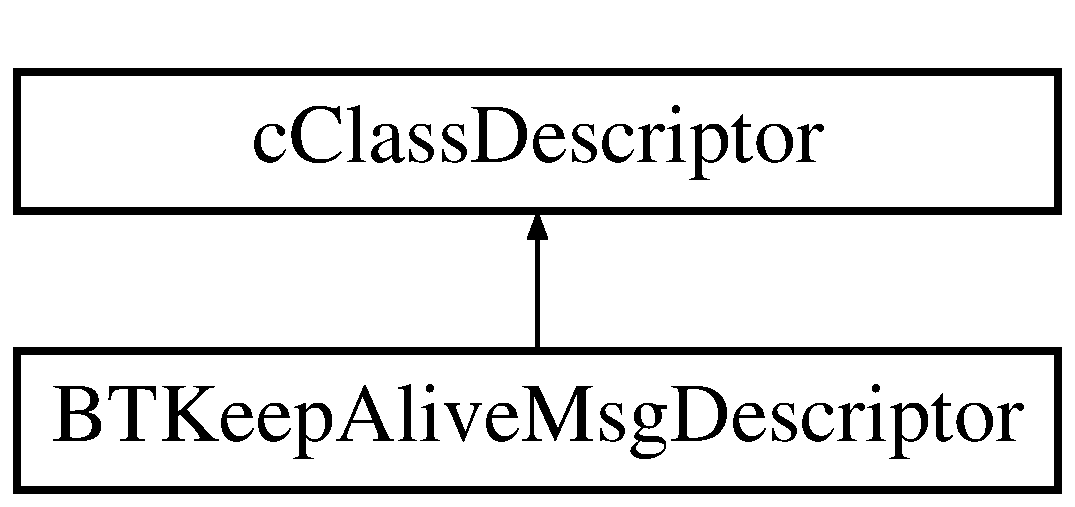
\includegraphics[height=2.000000cm]{classBTKeepAliveMsgDescriptor}
\end{center}
\end{figure}
\subsection*{Public Member Functions}
\begin{DoxyCompactItemize}
\item 
\hyperlink{classBTKeepAliveMsgDescriptor_a32954b8401791ef7557d0519a0cc9488}{B\+T\+Keep\+Alive\+Msg\+Descriptor} ()
\item 
virtual \hyperlink{classBTKeepAliveMsgDescriptor_a622963d1ad60fa8b47a22ad94040189d}{$\sim$\+B\+T\+Keep\+Alive\+Msg\+Descriptor} ()
\item 
virtual bool \hyperlink{classBTKeepAliveMsgDescriptor_a82ff2c0a6bbf981e760afee2ec460220}{does\+Support} (c\+Object $\ast$obj) const 
\item 
virtual const char $\ast$ \hyperlink{classBTKeepAliveMsgDescriptor_ad3aaa52b1900f71496d8afba2288ab67}{get\+Property} (const char $\ast$propertyname) const 
\item 
virtual int \hyperlink{classBTKeepAliveMsgDescriptor_a5d603f90b7f084e6a6839669d7ddf28c}{get\+Field\+Count} (void $\ast$object) const 
\item 
virtual const char $\ast$ \hyperlink{classBTKeepAliveMsgDescriptor_a61fe93534321bf88829616bfcfc54f16}{get\+Field\+Name} (void $\ast$object, int field) const 
\item 
virtual int \hyperlink{classBTKeepAliveMsgDescriptor_adb103eb1829ce42fba70f9265e029853}{find\+Field} (void $\ast$object, const char $\ast$field\+Name) const 
\item 
virtual unsigned int \hyperlink{classBTKeepAliveMsgDescriptor_ae3078013618e95fd61eec12295347ef3}{get\+Field\+Type\+Flags} (void $\ast$object, int field) const 
\item 
virtual const char $\ast$ \hyperlink{classBTKeepAliveMsgDescriptor_a9d0de7ec83b89da254a2f8251d26056a}{get\+Field\+Type\+String} (void $\ast$object, int field) const 
\item 
virtual const char $\ast$ \hyperlink{classBTKeepAliveMsgDescriptor_a7d875577fb00571df2890f00d42edd41}{get\+Field\+Property} (void $\ast$object, int field, const char $\ast$propertyname) const 
\item 
virtual int \hyperlink{classBTKeepAliveMsgDescriptor_aa53886b0b57af29a8da3e2d81ba7c03c}{get\+Array\+Size} (void $\ast$object, int field) const 
\item 
virtual std\+::string \hyperlink{classBTKeepAliveMsgDescriptor_a2a97c51fdf660891ee35df1dae409621}{get\+Field\+As\+String} (void $\ast$object, int field, int i) const 
\item 
virtual bool \hyperlink{classBTKeepAliveMsgDescriptor_ad8f3f532bf2eeb1668038c2e1d03c354}{set\+Field\+As\+String} (void $\ast$object, int field, int i, const char $\ast$value) const 
\item 
virtual const char $\ast$ \hyperlink{classBTKeepAliveMsgDescriptor_a3097b08d25a37e624341236d07080902}{get\+Field\+Struct\+Name} (void $\ast$object, int field) const 
\item 
virtual void $\ast$ \hyperlink{classBTKeepAliveMsgDescriptor_aa3cca28d5053a8c68971da657d603e53}{get\+Field\+Struct\+Pointer} (void $\ast$object, int field, int i) const 
\end{DoxyCompactItemize}


\subsection{Constructor \& Destructor Documentation}
\hypertarget{classBTKeepAliveMsgDescriptor_a32954b8401791ef7557d0519a0cc9488}{}\index{B\+T\+Keep\+Alive\+Msg\+Descriptor@{B\+T\+Keep\+Alive\+Msg\+Descriptor}!B\+T\+Keep\+Alive\+Msg\+Descriptor@{B\+T\+Keep\+Alive\+Msg\+Descriptor}}
\index{B\+T\+Keep\+Alive\+Msg\+Descriptor@{B\+T\+Keep\+Alive\+Msg\+Descriptor}!B\+T\+Keep\+Alive\+Msg\+Descriptor@{B\+T\+Keep\+Alive\+Msg\+Descriptor}}
\subsubsection[{B\+T\+Keep\+Alive\+Msg\+Descriptor()}]{\setlength{\rightskip}{0pt plus 5cm}B\+T\+Keep\+Alive\+Msg\+Descriptor\+::\+B\+T\+Keep\+Alive\+Msg\+Descriptor (
\begin{DoxyParamCaption}
{}
\end{DoxyParamCaption}
)}\label{classBTKeepAliveMsgDescriptor_a32954b8401791ef7557d0519a0cc9488}
\hypertarget{classBTKeepAliveMsgDescriptor_a622963d1ad60fa8b47a22ad94040189d}{}\index{B\+T\+Keep\+Alive\+Msg\+Descriptor@{B\+T\+Keep\+Alive\+Msg\+Descriptor}!````~B\+T\+Keep\+Alive\+Msg\+Descriptor@{$\sim$\+B\+T\+Keep\+Alive\+Msg\+Descriptor}}
\index{````~B\+T\+Keep\+Alive\+Msg\+Descriptor@{$\sim$\+B\+T\+Keep\+Alive\+Msg\+Descriptor}!B\+T\+Keep\+Alive\+Msg\+Descriptor@{B\+T\+Keep\+Alive\+Msg\+Descriptor}}
\subsubsection[{$\sim$\+B\+T\+Keep\+Alive\+Msg\+Descriptor()}]{\setlength{\rightskip}{0pt plus 5cm}B\+T\+Keep\+Alive\+Msg\+Descriptor\+::$\sim$\+B\+T\+Keep\+Alive\+Msg\+Descriptor (
\begin{DoxyParamCaption}
{}
\end{DoxyParamCaption}
)\hspace{0.3cm}{\ttfamily [virtual]}}\label{classBTKeepAliveMsgDescriptor_a622963d1ad60fa8b47a22ad94040189d}


\subsection{Member Function Documentation}
\hypertarget{classBTKeepAliveMsgDescriptor_a82ff2c0a6bbf981e760afee2ec460220}{}\index{B\+T\+Keep\+Alive\+Msg\+Descriptor@{B\+T\+Keep\+Alive\+Msg\+Descriptor}!does\+Support@{does\+Support}}
\index{does\+Support@{does\+Support}!B\+T\+Keep\+Alive\+Msg\+Descriptor@{B\+T\+Keep\+Alive\+Msg\+Descriptor}}
\subsubsection[{does\+Support(c\+Object $\ast$obj) const }]{\setlength{\rightskip}{0pt plus 5cm}bool B\+T\+Keep\+Alive\+Msg\+Descriptor\+::does\+Support (
\begin{DoxyParamCaption}
\item[{c\+Object $\ast$}]{obj}
\end{DoxyParamCaption}
) const\hspace{0.3cm}{\ttfamily [virtual]}}\label{classBTKeepAliveMsgDescriptor_a82ff2c0a6bbf981e760afee2ec460220}
\hypertarget{classBTKeepAliveMsgDescriptor_adb103eb1829ce42fba70f9265e029853}{}\index{B\+T\+Keep\+Alive\+Msg\+Descriptor@{B\+T\+Keep\+Alive\+Msg\+Descriptor}!find\+Field@{find\+Field}}
\index{find\+Field@{find\+Field}!B\+T\+Keep\+Alive\+Msg\+Descriptor@{B\+T\+Keep\+Alive\+Msg\+Descriptor}}
\subsubsection[{find\+Field(void $\ast$object, const char $\ast$field\+Name) const }]{\setlength{\rightskip}{0pt plus 5cm}int B\+T\+Keep\+Alive\+Msg\+Descriptor\+::find\+Field (
\begin{DoxyParamCaption}
\item[{void $\ast$}]{object, }
\item[{const char $\ast$}]{field\+Name}
\end{DoxyParamCaption}
) const\hspace{0.3cm}{\ttfamily [virtual]}}\label{classBTKeepAliveMsgDescriptor_adb103eb1829ce42fba70f9265e029853}
\hypertarget{classBTKeepAliveMsgDescriptor_aa53886b0b57af29a8da3e2d81ba7c03c}{}\index{B\+T\+Keep\+Alive\+Msg\+Descriptor@{B\+T\+Keep\+Alive\+Msg\+Descriptor}!get\+Array\+Size@{get\+Array\+Size}}
\index{get\+Array\+Size@{get\+Array\+Size}!B\+T\+Keep\+Alive\+Msg\+Descriptor@{B\+T\+Keep\+Alive\+Msg\+Descriptor}}
\subsubsection[{get\+Array\+Size(void $\ast$object, int field) const }]{\setlength{\rightskip}{0pt plus 5cm}int B\+T\+Keep\+Alive\+Msg\+Descriptor\+::get\+Array\+Size (
\begin{DoxyParamCaption}
\item[{void $\ast$}]{object, }
\item[{int}]{field}
\end{DoxyParamCaption}
) const\hspace{0.3cm}{\ttfamily [virtual]}}\label{classBTKeepAliveMsgDescriptor_aa53886b0b57af29a8da3e2d81ba7c03c}
\hypertarget{classBTKeepAliveMsgDescriptor_a2a97c51fdf660891ee35df1dae409621}{}\index{B\+T\+Keep\+Alive\+Msg\+Descriptor@{B\+T\+Keep\+Alive\+Msg\+Descriptor}!get\+Field\+As\+String@{get\+Field\+As\+String}}
\index{get\+Field\+As\+String@{get\+Field\+As\+String}!B\+T\+Keep\+Alive\+Msg\+Descriptor@{B\+T\+Keep\+Alive\+Msg\+Descriptor}}
\subsubsection[{get\+Field\+As\+String(void $\ast$object, int field, int i) const }]{\setlength{\rightskip}{0pt plus 5cm}std\+::string B\+T\+Keep\+Alive\+Msg\+Descriptor\+::get\+Field\+As\+String (
\begin{DoxyParamCaption}
\item[{void $\ast$}]{object, }
\item[{int}]{field, }
\item[{int}]{i}
\end{DoxyParamCaption}
) const\hspace{0.3cm}{\ttfamily [virtual]}}\label{classBTKeepAliveMsgDescriptor_a2a97c51fdf660891ee35df1dae409621}
\hypertarget{classBTKeepAliveMsgDescriptor_a5d603f90b7f084e6a6839669d7ddf28c}{}\index{B\+T\+Keep\+Alive\+Msg\+Descriptor@{B\+T\+Keep\+Alive\+Msg\+Descriptor}!get\+Field\+Count@{get\+Field\+Count}}
\index{get\+Field\+Count@{get\+Field\+Count}!B\+T\+Keep\+Alive\+Msg\+Descriptor@{B\+T\+Keep\+Alive\+Msg\+Descriptor}}
\subsubsection[{get\+Field\+Count(void $\ast$object) const }]{\setlength{\rightskip}{0pt plus 5cm}int B\+T\+Keep\+Alive\+Msg\+Descriptor\+::get\+Field\+Count (
\begin{DoxyParamCaption}
\item[{void $\ast$}]{object}
\end{DoxyParamCaption}
) const\hspace{0.3cm}{\ttfamily [virtual]}}\label{classBTKeepAliveMsgDescriptor_a5d603f90b7f084e6a6839669d7ddf28c}
\hypertarget{classBTKeepAliveMsgDescriptor_a61fe93534321bf88829616bfcfc54f16}{}\index{B\+T\+Keep\+Alive\+Msg\+Descriptor@{B\+T\+Keep\+Alive\+Msg\+Descriptor}!get\+Field\+Name@{get\+Field\+Name}}
\index{get\+Field\+Name@{get\+Field\+Name}!B\+T\+Keep\+Alive\+Msg\+Descriptor@{B\+T\+Keep\+Alive\+Msg\+Descriptor}}
\subsubsection[{get\+Field\+Name(void $\ast$object, int field) const }]{\setlength{\rightskip}{0pt plus 5cm}const char $\ast$ B\+T\+Keep\+Alive\+Msg\+Descriptor\+::get\+Field\+Name (
\begin{DoxyParamCaption}
\item[{void $\ast$}]{object, }
\item[{int}]{field}
\end{DoxyParamCaption}
) const\hspace{0.3cm}{\ttfamily [virtual]}}\label{classBTKeepAliveMsgDescriptor_a61fe93534321bf88829616bfcfc54f16}
\hypertarget{classBTKeepAliveMsgDescriptor_a7d875577fb00571df2890f00d42edd41}{}\index{B\+T\+Keep\+Alive\+Msg\+Descriptor@{B\+T\+Keep\+Alive\+Msg\+Descriptor}!get\+Field\+Property@{get\+Field\+Property}}
\index{get\+Field\+Property@{get\+Field\+Property}!B\+T\+Keep\+Alive\+Msg\+Descriptor@{B\+T\+Keep\+Alive\+Msg\+Descriptor}}
\subsubsection[{get\+Field\+Property(void $\ast$object, int field, const char $\ast$propertyname) const }]{\setlength{\rightskip}{0pt plus 5cm}const char $\ast$ B\+T\+Keep\+Alive\+Msg\+Descriptor\+::get\+Field\+Property (
\begin{DoxyParamCaption}
\item[{void $\ast$}]{object, }
\item[{int}]{field, }
\item[{const char $\ast$}]{propertyname}
\end{DoxyParamCaption}
) const\hspace{0.3cm}{\ttfamily [virtual]}}\label{classBTKeepAliveMsgDescriptor_a7d875577fb00571df2890f00d42edd41}
\hypertarget{classBTKeepAliveMsgDescriptor_a3097b08d25a37e624341236d07080902}{}\index{B\+T\+Keep\+Alive\+Msg\+Descriptor@{B\+T\+Keep\+Alive\+Msg\+Descriptor}!get\+Field\+Struct\+Name@{get\+Field\+Struct\+Name}}
\index{get\+Field\+Struct\+Name@{get\+Field\+Struct\+Name}!B\+T\+Keep\+Alive\+Msg\+Descriptor@{B\+T\+Keep\+Alive\+Msg\+Descriptor}}
\subsubsection[{get\+Field\+Struct\+Name(void $\ast$object, int field) const }]{\setlength{\rightskip}{0pt plus 5cm}const char $\ast$ B\+T\+Keep\+Alive\+Msg\+Descriptor\+::get\+Field\+Struct\+Name (
\begin{DoxyParamCaption}
\item[{void $\ast$}]{object, }
\item[{int}]{field}
\end{DoxyParamCaption}
) const\hspace{0.3cm}{\ttfamily [virtual]}}\label{classBTKeepAliveMsgDescriptor_a3097b08d25a37e624341236d07080902}
\hypertarget{classBTKeepAliveMsgDescriptor_aa3cca28d5053a8c68971da657d603e53}{}\index{B\+T\+Keep\+Alive\+Msg\+Descriptor@{B\+T\+Keep\+Alive\+Msg\+Descriptor}!get\+Field\+Struct\+Pointer@{get\+Field\+Struct\+Pointer}}
\index{get\+Field\+Struct\+Pointer@{get\+Field\+Struct\+Pointer}!B\+T\+Keep\+Alive\+Msg\+Descriptor@{B\+T\+Keep\+Alive\+Msg\+Descriptor}}
\subsubsection[{get\+Field\+Struct\+Pointer(void $\ast$object, int field, int i) const }]{\setlength{\rightskip}{0pt plus 5cm}void $\ast$ B\+T\+Keep\+Alive\+Msg\+Descriptor\+::get\+Field\+Struct\+Pointer (
\begin{DoxyParamCaption}
\item[{void $\ast$}]{object, }
\item[{int}]{field, }
\item[{int}]{i}
\end{DoxyParamCaption}
) const\hspace{0.3cm}{\ttfamily [virtual]}}\label{classBTKeepAliveMsgDescriptor_aa3cca28d5053a8c68971da657d603e53}
\hypertarget{classBTKeepAliveMsgDescriptor_ae3078013618e95fd61eec12295347ef3}{}\index{B\+T\+Keep\+Alive\+Msg\+Descriptor@{B\+T\+Keep\+Alive\+Msg\+Descriptor}!get\+Field\+Type\+Flags@{get\+Field\+Type\+Flags}}
\index{get\+Field\+Type\+Flags@{get\+Field\+Type\+Flags}!B\+T\+Keep\+Alive\+Msg\+Descriptor@{B\+T\+Keep\+Alive\+Msg\+Descriptor}}
\subsubsection[{get\+Field\+Type\+Flags(void $\ast$object, int field) const }]{\setlength{\rightskip}{0pt plus 5cm}unsigned int B\+T\+Keep\+Alive\+Msg\+Descriptor\+::get\+Field\+Type\+Flags (
\begin{DoxyParamCaption}
\item[{void $\ast$}]{object, }
\item[{int}]{field}
\end{DoxyParamCaption}
) const\hspace{0.3cm}{\ttfamily [virtual]}}\label{classBTKeepAliveMsgDescriptor_ae3078013618e95fd61eec12295347ef3}
\hypertarget{classBTKeepAliveMsgDescriptor_a9d0de7ec83b89da254a2f8251d26056a}{}\index{B\+T\+Keep\+Alive\+Msg\+Descriptor@{B\+T\+Keep\+Alive\+Msg\+Descriptor}!get\+Field\+Type\+String@{get\+Field\+Type\+String}}
\index{get\+Field\+Type\+String@{get\+Field\+Type\+String}!B\+T\+Keep\+Alive\+Msg\+Descriptor@{B\+T\+Keep\+Alive\+Msg\+Descriptor}}
\subsubsection[{get\+Field\+Type\+String(void $\ast$object, int field) const }]{\setlength{\rightskip}{0pt plus 5cm}const char $\ast$ B\+T\+Keep\+Alive\+Msg\+Descriptor\+::get\+Field\+Type\+String (
\begin{DoxyParamCaption}
\item[{void $\ast$}]{object, }
\item[{int}]{field}
\end{DoxyParamCaption}
) const\hspace{0.3cm}{\ttfamily [virtual]}}\label{classBTKeepAliveMsgDescriptor_a9d0de7ec83b89da254a2f8251d26056a}
\hypertarget{classBTKeepAliveMsgDescriptor_ad3aaa52b1900f71496d8afba2288ab67}{}\index{B\+T\+Keep\+Alive\+Msg\+Descriptor@{B\+T\+Keep\+Alive\+Msg\+Descriptor}!get\+Property@{get\+Property}}
\index{get\+Property@{get\+Property}!B\+T\+Keep\+Alive\+Msg\+Descriptor@{B\+T\+Keep\+Alive\+Msg\+Descriptor}}
\subsubsection[{get\+Property(const char $\ast$propertyname) const }]{\setlength{\rightskip}{0pt plus 5cm}const char $\ast$ B\+T\+Keep\+Alive\+Msg\+Descriptor\+::get\+Property (
\begin{DoxyParamCaption}
\item[{const char $\ast$}]{propertyname}
\end{DoxyParamCaption}
) const\hspace{0.3cm}{\ttfamily [virtual]}}\label{classBTKeepAliveMsgDescriptor_ad3aaa52b1900f71496d8afba2288ab67}
\hypertarget{classBTKeepAliveMsgDescriptor_ad8f3f532bf2eeb1668038c2e1d03c354}{}\index{B\+T\+Keep\+Alive\+Msg\+Descriptor@{B\+T\+Keep\+Alive\+Msg\+Descriptor}!set\+Field\+As\+String@{set\+Field\+As\+String}}
\index{set\+Field\+As\+String@{set\+Field\+As\+String}!B\+T\+Keep\+Alive\+Msg\+Descriptor@{B\+T\+Keep\+Alive\+Msg\+Descriptor}}
\subsubsection[{set\+Field\+As\+String(void $\ast$object, int field, int i, const char $\ast$value) const }]{\setlength{\rightskip}{0pt plus 5cm}bool B\+T\+Keep\+Alive\+Msg\+Descriptor\+::set\+Field\+As\+String (
\begin{DoxyParamCaption}
\item[{void $\ast$}]{object, }
\item[{int}]{field, }
\item[{int}]{i, }
\item[{const char $\ast$}]{value}
\end{DoxyParamCaption}
) const\hspace{0.3cm}{\ttfamily [virtual]}}\label{classBTKeepAliveMsgDescriptor_ad8f3f532bf2eeb1668038c2e1d03c354}


The documentation for this class was generated from the following file\+:\begin{DoxyCompactItemize}
\item 
\hyperlink{BTPeerWireMsg__m_8cc}{B\+T\+Peer\+Wire\+Msg\+\_\+m.\+cc}\end{DoxyCompactItemize}

\hypertarget{classBTMsgHandshake}{}\section{B\+T\+Msg\+Handshake Class Reference}
\label{classBTMsgHandshake}\index{B\+T\+Msg\+Handshake@{B\+T\+Msg\+Handshake}}


{\ttfamily \#include $<$B\+T\+Peer\+Wire\+Msg\+\_\+m.\+h$>$}

Inheritance diagram for B\+T\+Msg\+Handshake\+:\begin{figure}[H]
\begin{center}
\leavevmode
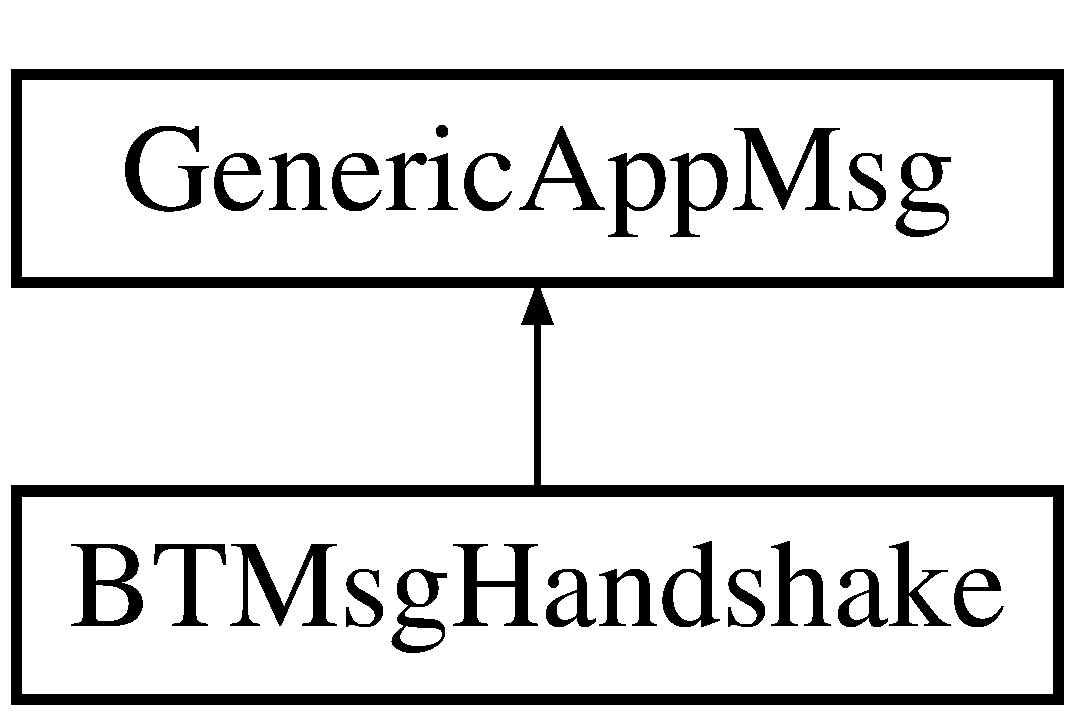
\includegraphics[height=2.000000cm]{classBTMsgHandshake}
\end{center}
\end{figure}
\subsection*{Public Member Functions}
\begin{DoxyCompactItemize}
\item 
\hyperlink{classBTMsgHandshake_a3647388b293bcfe86ee4d3d6978499dd}{B\+T\+Msg\+Handshake} (const char $\ast$name=N\+U\+L\+L, int kind=0)
\item 
\hyperlink{classBTMsgHandshake_aabdd16aad5b8045597daa66ae351da79}{B\+T\+Msg\+Handshake} (const \hyperlink{classBTMsgHandshake}{B\+T\+Msg\+Handshake} \&other)
\item 
virtual \hyperlink{classBTMsgHandshake_a769ddebed475d96a9e98af23442c18a0}{$\sim$\+B\+T\+Msg\+Handshake} ()
\item 
\hyperlink{classBTMsgHandshake}{B\+T\+Msg\+Handshake} \& \hyperlink{classBTMsgHandshake_a31bab774b8a182471abf501acfcedc4a}{operator=} (const \hyperlink{classBTMsgHandshake}{B\+T\+Msg\+Handshake} \&other)
\item 
virtual \hyperlink{classBTMsgHandshake}{B\+T\+Msg\+Handshake} $\ast$ \hyperlink{classBTMsgHandshake_a5dc5693ae117aae06ee66308974c0623}{dup} () const 
\item 
virtual void \hyperlink{classBTMsgHandshake_ad8c48e46aa80079dff589d99fafdc637}{parsim\+Pack} (c\+Comm\+Buffer $\ast$b)
\item 
virtual void \hyperlink{classBTMsgHandshake_afd07f5ee1198c520ba32f9ac9fdfd060}{parsim\+Unpack} (c\+Comm\+Buffer $\ast$b)
\item 
virtual char \hyperlink{classBTMsgHandshake_a25c0d32b72fde124d1b6c57965df964f}{pstrlen} () const 
\item 
virtual void \hyperlink{classBTMsgHandshake_a9b81e33ee9cfe17c04a9dd41214860c5}{set\+Pstrlen} (char \hyperlink{classBTMsgHandshake_aac6817b686487e3646ff1ec8ffe28965}{pstrlen\+\_\+var})
\item 
virtual const char $\ast$ \hyperlink{classBTMsgHandshake_a0b8d1d3f7aabc420d382089767833b5b}{pstr} () const 
\item 
virtual void \hyperlink{classBTMsgHandshake_a2e8a2858b089b1fa12c2bda68f64390a}{set\+Pstr} (const char $\ast$\hyperlink{classBTMsgHandshake_a913d64395dfd4230c77881950871df18}{pstr\+\_\+var})
\item 
virtual unsigned int \hyperlink{classBTMsgHandshake_a2e850e68903d55d95dc64a7c3db48fe4}{reserved\+Array\+Size} () const 
\item 
virtual bool \hyperlink{classBTMsgHandshake_a9c39003dbbd8c136928073e77a51a403}{reserved} (unsigned int k) const 
\item 
virtual void \hyperlink{classBTMsgHandshake_ade2372fe17094b3aefc6bb5bd6d32bbd}{set\+Reserved} (unsigned int k, bool \hyperlink{classBTMsgHandshake_a289f010d689e2d2649e1585c6eb8a683}{reserved\+\_\+var})
\item 
virtual const char $\ast$ \hyperlink{classBTMsgHandshake_a5a74e2bd313765bcb504119e97d80a47}{info\+Hash} () const 
\item 
virtual void \hyperlink{classBTMsgHandshake_a546d2963e8e7e8066bceb00e1e4d1df2}{set\+Info\+Hash} (const char $\ast$\hyperlink{classBTMsgHandshake_a6c79f9de6d2c47ecf9a1f7172ce10bef}{info\+Hash\+\_\+var})
\item 
virtual const char $\ast$ \hyperlink{classBTMsgHandshake_ab9e8f0a422844b270542b94813f6d564}{peer\+Id} () const 
\item 
virtual void \hyperlink{classBTMsgHandshake_a0556438c3711ed78b72732942f357585}{set\+Peer\+Id} (const char $\ast$\hyperlink{classBTMsgHandshake_a269237a5af72db85d27cd1080e998cd8}{peer\+Id\+\_\+var})
\end{DoxyCompactItemize}
\subsection*{Protected Member Functions}
\begin{DoxyCompactItemize}
\item 
bool \hyperlink{classBTMsgHandshake_ad8a228811e1c2fc12272a7d263becef2}{operator==} (const \hyperlink{classBTMsgHandshake}{B\+T\+Msg\+Handshake} \&)
\end{DoxyCompactItemize}
\subsection*{Protected Attributes}
\begin{DoxyCompactItemize}
\item 
char \hyperlink{classBTMsgHandshake_aac6817b686487e3646ff1ec8ffe28965}{pstrlen\+\_\+var}
\item 
opp\+\_\+string \hyperlink{classBTMsgHandshake_a913d64395dfd4230c77881950871df18}{pstr\+\_\+var}
\item 
bool \hyperlink{classBTMsgHandshake_a289f010d689e2d2649e1585c6eb8a683}{reserved\+\_\+var} \mbox{[}8\mbox{]}
\item 
opp\+\_\+string \hyperlink{classBTMsgHandshake_a6c79f9de6d2c47ecf9a1f7172ce10bef}{info\+Hash\+\_\+var}
\item 
opp\+\_\+string \hyperlink{classBTMsgHandshake_a269237a5af72db85d27cd1080e998cd8}{peer\+Id\+\_\+var}
\end{DoxyCompactItemize}


\subsection{Detailed Description}
Class generated from {\ttfamily applications/x\+Bit\+Torrent/\+B\+T\+Peer\+Wire\+Msg.\+msg} by opp\+\_\+msgc. 
\begin{DoxyPre}
message \hyperlink{classBTMsgHandshake}{BTMsgHandshake} extends GenericAppMsg
\{
    (true);\end{DoxyPre}



\begin{DoxyPre}    char pstrlen;       
    string pstr;
    bool reserved[8];
    string infoHash;
    string peerId;\end{DoxyPre}



\begin{DoxyPre}\}
\end{DoxyPre}
 

\subsection{Constructor \& Destructor Documentation}
\hypertarget{classBTMsgHandshake_a3647388b293bcfe86ee4d3d6978499dd}{}\index{B\+T\+Msg\+Handshake@{B\+T\+Msg\+Handshake}!B\+T\+Msg\+Handshake@{B\+T\+Msg\+Handshake}}
\index{B\+T\+Msg\+Handshake@{B\+T\+Msg\+Handshake}!B\+T\+Msg\+Handshake@{B\+T\+Msg\+Handshake}}
\subsubsection[{B\+T\+Msg\+Handshake(const char $\ast$name=\+N\+U\+L\+L, int kind=0)}]{\setlength{\rightskip}{0pt plus 5cm}B\+T\+Msg\+Handshake\+::\+B\+T\+Msg\+Handshake (
\begin{DoxyParamCaption}
\item[{const char $\ast$}]{name = {\ttfamily NULL}, }
\item[{int}]{kind = {\ttfamily 0}}
\end{DoxyParamCaption}
)}\label{classBTMsgHandshake_a3647388b293bcfe86ee4d3d6978499dd}
\hypertarget{classBTMsgHandshake_aabdd16aad5b8045597daa66ae351da79}{}\index{B\+T\+Msg\+Handshake@{B\+T\+Msg\+Handshake}!B\+T\+Msg\+Handshake@{B\+T\+Msg\+Handshake}}
\index{B\+T\+Msg\+Handshake@{B\+T\+Msg\+Handshake}!B\+T\+Msg\+Handshake@{B\+T\+Msg\+Handshake}}
\subsubsection[{B\+T\+Msg\+Handshake(const B\+T\+Msg\+Handshake \&other)}]{\setlength{\rightskip}{0pt plus 5cm}B\+T\+Msg\+Handshake\+::\+B\+T\+Msg\+Handshake (
\begin{DoxyParamCaption}
\item[{const {\bf B\+T\+Msg\+Handshake} \&}]{other}
\end{DoxyParamCaption}
)}\label{classBTMsgHandshake_aabdd16aad5b8045597daa66ae351da79}
\hypertarget{classBTMsgHandshake_a769ddebed475d96a9e98af23442c18a0}{}\index{B\+T\+Msg\+Handshake@{B\+T\+Msg\+Handshake}!````~B\+T\+Msg\+Handshake@{$\sim$\+B\+T\+Msg\+Handshake}}
\index{````~B\+T\+Msg\+Handshake@{$\sim$\+B\+T\+Msg\+Handshake}!B\+T\+Msg\+Handshake@{B\+T\+Msg\+Handshake}}
\subsubsection[{$\sim$\+B\+T\+Msg\+Handshake()}]{\setlength{\rightskip}{0pt plus 5cm}B\+T\+Msg\+Handshake\+::$\sim$\+B\+T\+Msg\+Handshake (
\begin{DoxyParamCaption}
{}
\end{DoxyParamCaption}
)\hspace{0.3cm}{\ttfamily [virtual]}}\label{classBTMsgHandshake_a769ddebed475d96a9e98af23442c18a0}


\subsection{Member Function Documentation}
\hypertarget{classBTMsgHandshake_a5dc5693ae117aae06ee66308974c0623}{}\index{B\+T\+Msg\+Handshake@{B\+T\+Msg\+Handshake}!dup@{dup}}
\index{dup@{dup}!B\+T\+Msg\+Handshake@{B\+T\+Msg\+Handshake}}
\subsubsection[{dup() const }]{\setlength{\rightskip}{0pt plus 5cm}virtual {\bf B\+T\+Msg\+Handshake}$\ast$ B\+T\+Msg\+Handshake\+::dup (
\begin{DoxyParamCaption}
{}
\end{DoxyParamCaption}
) const\hspace{0.3cm}{\ttfamily [inline]}, {\ttfamily [virtual]}}\label{classBTMsgHandshake_a5dc5693ae117aae06ee66308974c0623}
\hypertarget{classBTMsgHandshake_a5a74e2bd313765bcb504119e97d80a47}{}\index{B\+T\+Msg\+Handshake@{B\+T\+Msg\+Handshake}!info\+Hash@{info\+Hash}}
\index{info\+Hash@{info\+Hash}!B\+T\+Msg\+Handshake@{B\+T\+Msg\+Handshake}}
\subsubsection[{info\+Hash() const }]{\setlength{\rightskip}{0pt plus 5cm}const char $\ast$ B\+T\+Msg\+Handshake\+::info\+Hash (
\begin{DoxyParamCaption}
{}
\end{DoxyParamCaption}
) const\hspace{0.3cm}{\ttfamily [virtual]}}\label{classBTMsgHandshake_a5a74e2bd313765bcb504119e97d80a47}
\hypertarget{classBTMsgHandshake_a31bab774b8a182471abf501acfcedc4a}{}\index{B\+T\+Msg\+Handshake@{B\+T\+Msg\+Handshake}!operator=@{operator=}}
\index{operator=@{operator=}!B\+T\+Msg\+Handshake@{B\+T\+Msg\+Handshake}}
\subsubsection[{operator=(const B\+T\+Msg\+Handshake \&other)}]{\setlength{\rightskip}{0pt plus 5cm}{\bf B\+T\+Msg\+Handshake} \& B\+T\+Msg\+Handshake\+::operator= (
\begin{DoxyParamCaption}
\item[{const {\bf B\+T\+Msg\+Handshake} \&}]{other}
\end{DoxyParamCaption}
)}\label{classBTMsgHandshake_a31bab774b8a182471abf501acfcedc4a}
\hypertarget{classBTMsgHandshake_ad8a228811e1c2fc12272a7d263becef2}{}\index{B\+T\+Msg\+Handshake@{B\+T\+Msg\+Handshake}!operator==@{operator==}}
\index{operator==@{operator==}!B\+T\+Msg\+Handshake@{B\+T\+Msg\+Handshake}}
\subsubsection[{operator==(const B\+T\+Msg\+Handshake \&)}]{\setlength{\rightskip}{0pt plus 5cm}bool B\+T\+Msg\+Handshake\+::operator== (
\begin{DoxyParamCaption}
\item[{const {\bf B\+T\+Msg\+Handshake} \&}]{}
\end{DoxyParamCaption}
)\hspace{0.3cm}{\ttfamily [protected]}}\label{classBTMsgHandshake_ad8a228811e1c2fc12272a7d263becef2}
\hypertarget{classBTMsgHandshake_ad8c48e46aa80079dff589d99fafdc637}{}\index{B\+T\+Msg\+Handshake@{B\+T\+Msg\+Handshake}!parsim\+Pack@{parsim\+Pack}}
\index{parsim\+Pack@{parsim\+Pack}!B\+T\+Msg\+Handshake@{B\+T\+Msg\+Handshake}}
\subsubsection[{parsim\+Pack(c\+Comm\+Buffer $\ast$b)}]{\setlength{\rightskip}{0pt plus 5cm}void B\+T\+Msg\+Handshake\+::parsim\+Pack (
\begin{DoxyParamCaption}
\item[{c\+Comm\+Buffer $\ast$}]{b}
\end{DoxyParamCaption}
)\hspace{0.3cm}{\ttfamily [virtual]}}\label{classBTMsgHandshake_ad8c48e46aa80079dff589d99fafdc637}
\hypertarget{classBTMsgHandshake_afd07f5ee1198c520ba32f9ac9fdfd060}{}\index{B\+T\+Msg\+Handshake@{B\+T\+Msg\+Handshake}!parsim\+Unpack@{parsim\+Unpack}}
\index{parsim\+Unpack@{parsim\+Unpack}!B\+T\+Msg\+Handshake@{B\+T\+Msg\+Handshake}}
\subsubsection[{parsim\+Unpack(c\+Comm\+Buffer $\ast$b)}]{\setlength{\rightskip}{0pt plus 5cm}void B\+T\+Msg\+Handshake\+::parsim\+Unpack (
\begin{DoxyParamCaption}
\item[{c\+Comm\+Buffer $\ast$}]{b}
\end{DoxyParamCaption}
)\hspace{0.3cm}{\ttfamily [virtual]}}\label{classBTMsgHandshake_afd07f5ee1198c520ba32f9ac9fdfd060}
\hypertarget{classBTMsgHandshake_ab9e8f0a422844b270542b94813f6d564}{}\index{B\+T\+Msg\+Handshake@{B\+T\+Msg\+Handshake}!peer\+Id@{peer\+Id}}
\index{peer\+Id@{peer\+Id}!B\+T\+Msg\+Handshake@{B\+T\+Msg\+Handshake}}
\subsubsection[{peer\+Id() const }]{\setlength{\rightskip}{0pt plus 5cm}const char $\ast$ B\+T\+Msg\+Handshake\+::peer\+Id (
\begin{DoxyParamCaption}
{}
\end{DoxyParamCaption}
) const\hspace{0.3cm}{\ttfamily [virtual]}}\label{classBTMsgHandshake_ab9e8f0a422844b270542b94813f6d564}
\hypertarget{classBTMsgHandshake_a0b8d1d3f7aabc420d382089767833b5b}{}\index{B\+T\+Msg\+Handshake@{B\+T\+Msg\+Handshake}!pstr@{pstr}}
\index{pstr@{pstr}!B\+T\+Msg\+Handshake@{B\+T\+Msg\+Handshake}}
\subsubsection[{pstr() const }]{\setlength{\rightskip}{0pt plus 5cm}const char $\ast$ B\+T\+Msg\+Handshake\+::pstr (
\begin{DoxyParamCaption}
{}
\end{DoxyParamCaption}
) const\hspace{0.3cm}{\ttfamily [virtual]}}\label{classBTMsgHandshake_a0b8d1d3f7aabc420d382089767833b5b}
\hypertarget{classBTMsgHandshake_a25c0d32b72fde124d1b6c57965df964f}{}\index{B\+T\+Msg\+Handshake@{B\+T\+Msg\+Handshake}!pstrlen@{pstrlen}}
\index{pstrlen@{pstrlen}!B\+T\+Msg\+Handshake@{B\+T\+Msg\+Handshake}}
\subsubsection[{pstrlen() const }]{\setlength{\rightskip}{0pt plus 5cm}char B\+T\+Msg\+Handshake\+::pstrlen (
\begin{DoxyParamCaption}
{}
\end{DoxyParamCaption}
) const\hspace{0.3cm}{\ttfamily [virtual]}}\label{classBTMsgHandshake_a25c0d32b72fde124d1b6c57965df964f}
\hypertarget{classBTMsgHandshake_a9c39003dbbd8c136928073e77a51a403}{}\index{B\+T\+Msg\+Handshake@{B\+T\+Msg\+Handshake}!reserved@{reserved}}
\index{reserved@{reserved}!B\+T\+Msg\+Handshake@{B\+T\+Msg\+Handshake}}
\subsubsection[{reserved(unsigned int k) const }]{\setlength{\rightskip}{0pt plus 5cm}bool B\+T\+Msg\+Handshake\+::reserved (
\begin{DoxyParamCaption}
\item[{unsigned int}]{k}
\end{DoxyParamCaption}
) const\hspace{0.3cm}{\ttfamily [virtual]}}\label{classBTMsgHandshake_a9c39003dbbd8c136928073e77a51a403}
\hypertarget{classBTMsgHandshake_a2e850e68903d55d95dc64a7c3db48fe4}{}\index{B\+T\+Msg\+Handshake@{B\+T\+Msg\+Handshake}!reserved\+Array\+Size@{reserved\+Array\+Size}}
\index{reserved\+Array\+Size@{reserved\+Array\+Size}!B\+T\+Msg\+Handshake@{B\+T\+Msg\+Handshake}}
\subsubsection[{reserved\+Array\+Size() const }]{\setlength{\rightskip}{0pt plus 5cm}unsigned int B\+T\+Msg\+Handshake\+::reserved\+Array\+Size (
\begin{DoxyParamCaption}
{}
\end{DoxyParamCaption}
) const\hspace{0.3cm}{\ttfamily [virtual]}}\label{classBTMsgHandshake_a2e850e68903d55d95dc64a7c3db48fe4}
\hypertarget{classBTMsgHandshake_a546d2963e8e7e8066bceb00e1e4d1df2}{}\index{B\+T\+Msg\+Handshake@{B\+T\+Msg\+Handshake}!set\+Info\+Hash@{set\+Info\+Hash}}
\index{set\+Info\+Hash@{set\+Info\+Hash}!B\+T\+Msg\+Handshake@{B\+T\+Msg\+Handshake}}
\subsubsection[{set\+Info\+Hash(const char $\ast$info\+Hash\+\_\+var)}]{\setlength{\rightskip}{0pt plus 5cm}void B\+T\+Msg\+Handshake\+::set\+Info\+Hash (
\begin{DoxyParamCaption}
\item[{const char $\ast$}]{info\+Hash\+\_\+var}
\end{DoxyParamCaption}
)\hspace{0.3cm}{\ttfamily [virtual]}}\label{classBTMsgHandshake_a546d2963e8e7e8066bceb00e1e4d1df2}
\hypertarget{classBTMsgHandshake_a0556438c3711ed78b72732942f357585}{}\index{B\+T\+Msg\+Handshake@{B\+T\+Msg\+Handshake}!set\+Peer\+Id@{set\+Peer\+Id}}
\index{set\+Peer\+Id@{set\+Peer\+Id}!B\+T\+Msg\+Handshake@{B\+T\+Msg\+Handshake}}
\subsubsection[{set\+Peer\+Id(const char $\ast$peer\+Id\+\_\+var)}]{\setlength{\rightskip}{0pt plus 5cm}void B\+T\+Msg\+Handshake\+::set\+Peer\+Id (
\begin{DoxyParamCaption}
\item[{const char $\ast$}]{peer\+Id\+\_\+var}
\end{DoxyParamCaption}
)\hspace{0.3cm}{\ttfamily [virtual]}}\label{classBTMsgHandshake_a0556438c3711ed78b72732942f357585}
\hypertarget{classBTMsgHandshake_a2e8a2858b089b1fa12c2bda68f64390a}{}\index{B\+T\+Msg\+Handshake@{B\+T\+Msg\+Handshake}!set\+Pstr@{set\+Pstr}}
\index{set\+Pstr@{set\+Pstr}!B\+T\+Msg\+Handshake@{B\+T\+Msg\+Handshake}}
\subsubsection[{set\+Pstr(const char $\ast$pstr\+\_\+var)}]{\setlength{\rightskip}{0pt plus 5cm}void B\+T\+Msg\+Handshake\+::set\+Pstr (
\begin{DoxyParamCaption}
\item[{const char $\ast$}]{pstr\+\_\+var}
\end{DoxyParamCaption}
)\hspace{0.3cm}{\ttfamily [virtual]}}\label{classBTMsgHandshake_a2e8a2858b089b1fa12c2bda68f64390a}
\hypertarget{classBTMsgHandshake_a9b81e33ee9cfe17c04a9dd41214860c5}{}\index{B\+T\+Msg\+Handshake@{B\+T\+Msg\+Handshake}!set\+Pstrlen@{set\+Pstrlen}}
\index{set\+Pstrlen@{set\+Pstrlen}!B\+T\+Msg\+Handshake@{B\+T\+Msg\+Handshake}}
\subsubsection[{set\+Pstrlen(char pstrlen\+\_\+var)}]{\setlength{\rightskip}{0pt plus 5cm}void B\+T\+Msg\+Handshake\+::set\+Pstrlen (
\begin{DoxyParamCaption}
\item[{char}]{pstrlen\+\_\+var}
\end{DoxyParamCaption}
)\hspace{0.3cm}{\ttfamily [virtual]}}\label{classBTMsgHandshake_a9b81e33ee9cfe17c04a9dd41214860c5}
\hypertarget{classBTMsgHandshake_ade2372fe17094b3aefc6bb5bd6d32bbd}{}\index{B\+T\+Msg\+Handshake@{B\+T\+Msg\+Handshake}!set\+Reserved@{set\+Reserved}}
\index{set\+Reserved@{set\+Reserved}!B\+T\+Msg\+Handshake@{B\+T\+Msg\+Handshake}}
\subsubsection[{set\+Reserved(unsigned int k, bool reserved\+\_\+var)}]{\setlength{\rightskip}{0pt plus 5cm}void B\+T\+Msg\+Handshake\+::set\+Reserved (
\begin{DoxyParamCaption}
\item[{unsigned int}]{k, }
\item[{bool}]{reserved\+\_\+var}
\end{DoxyParamCaption}
)\hspace{0.3cm}{\ttfamily [virtual]}}\label{classBTMsgHandshake_ade2372fe17094b3aefc6bb5bd6d32bbd}


\subsection{Member Data Documentation}
\hypertarget{classBTMsgHandshake_a6c79f9de6d2c47ecf9a1f7172ce10bef}{}\index{B\+T\+Msg\+Handshake@{B\+T\+Msg\+Handshake}!info\+Hash\+\_\+var@{info\+Hash\+\_\+var}}
\index{info\+Hash\+\_\+var@{info\+Hash\+\_\+var}!B\+T\+Msg\+Handshake@{B\+T\+Msg\+Handshake}}
\subsubsection[{info\+Hash\+\_\+var}]{\setlength{\rightskip}{0pt plus 5cm}opp\+\_\+string B\+T\+Msg\+Handshake\+::info\+Hash\+\_\+var\hspace{0.3cm}{\ttfamily [protected]}}\label{classBTMsgHandshake_a6c79f9de6d2c47ecf9a1f7172ce10bef}
\hypertarget{classBTMsgHandshake_a269237a5af72db85d27cd1080e998cd8}{}\index{B\+T\+Msg\+Handshake@{B\+T\+Msg\+Handshake}!peer\+Id\+\_\+var@{peer\+Id\+\_\+var}}
\index{peer\+Id\+\_\+var@{peer\+Id\+\_\+var}!B\+T\+Msg\+Handshake@{B\+T\+Msg\+Handshake}}
\subsubsection[{peer\+Id\+\_\+var}]{\setlength{\rightskip}{0pt plus 5cm}opp\+\_\+string B\+T\+Msg\+Handshake\+::peer\+Id\+\_\+var\hspace{0.3cm}{\ttfamily [protected]}}\label{classBTMsgHandshake_a269237a5af72db85d27cd1080e998cd8}
\hypertarget{classBTMsgHandshake_a913d64395dfd4230c77881950871df18}{}\index{B\+T\+Msg\+Handshake@{B\+T\+Msg\+Handshake}!pstr\+\_\+var@{pstr\+\_\+var}}
\index{pstr\+\_\+var@{pstr\+\_\+var}!B\+T\+Msg\+Handshake@{B\+T\+Msg\+Handshake}}
\subsubsection[{pstr\+\_\+var}]{\setlength{\rightskip}{0pt plus 5cm}opp\+\_\+string B\+T\+Msg\+Handshake\+::pstr\+\_\+var\hspace{0.3cm}{\ttfamily [protected]}}\label{classBTMsgHandshake_a913d64395dfd4230c77881950871df18}
\hypertarget{classBTMsgHandshake_aac6817b686487e3646ff1ec8ffe28965}{}\index{B\+T\+Msg\+Handshake@{B\+T\+Msg\+Handshake}!pstrlen\+\_\+var@{pstrlen\+\_\+var}}
\index{pstrlen\+\_\+var@{pstrlen\+\_\+var}!B\+T\+Msg\+Handshake@{B\+T\+Msg\+Handshake}}
\subsubsection[{pstrlen\+\_\+var}]{\setlength{\rightskip}{0pt plus 5cm}char B\+T\+Msg\+Handshake\+::pstrlen\+\_\+var\hspace{0.3cm}{\ttfamily [protected]}}\label{classBTMsgHandshake_aac6817b686487e3646ff1ec8ffe28965}
\hypertarget{classBTMsgHandshake_a289f010d689e2d2649e1585c6eb8a683}{}\index{B\+T\+Msg\+Handshake@{B\+T\+Msg\+Handshake}!reserved\+\_\+var@{reserved\+\_\+var}}
\index{reserved\+\_\+var@{reserved\+\_\+var}!B\+T\+Msg\+Handshake@{B\+T\+Msg\+Handshake}}
\subsubsection[{reserved\+\_\+var}]{\setlength{\rightskip}{0pt plus 5cm}bool B\+T\+Msg\+Handshake\+::reserved\+\_\+var\mbox{[}8\mbox{]}\hspace{0.3cm}{\ttfamily [protected]}}\label{classBTMsgHandshake_a289f010d689e2d2649e1585c6eb8a683}


The documentation for this class was generated from the following files\+:\begin{DoxyCompactItemize}
\item 
\hyperlink{BTPeerWireMsg__m_8h}{B\+T\+Peer\+Wire\+Msg\+\_\+m.\+h}\item 
\hyperlink{BTPeerWireMsg__m_8cc}{B\+T\+Peer\+Wire\+Msg\+\_\+m.\+cc}\end{DoxyCompactItemize}

\hypertarget{classBTMsgHandshakeDescriptor}{}\section{B\+T\+Msg\+Handshake\+Descriptor Class Reference}
\label{classBTMsgHandshakeDescriptor}\index{B\+T\+Msg\+Handshake\+Descriptor@{B\+T\+Msg\+Handshake\+Descriptor}}
Inheritance diagram for B\+T\+Msg\+Handshake\+Descriptor\+:\begin{figure}[H]
\begin{center}
\leavevmode
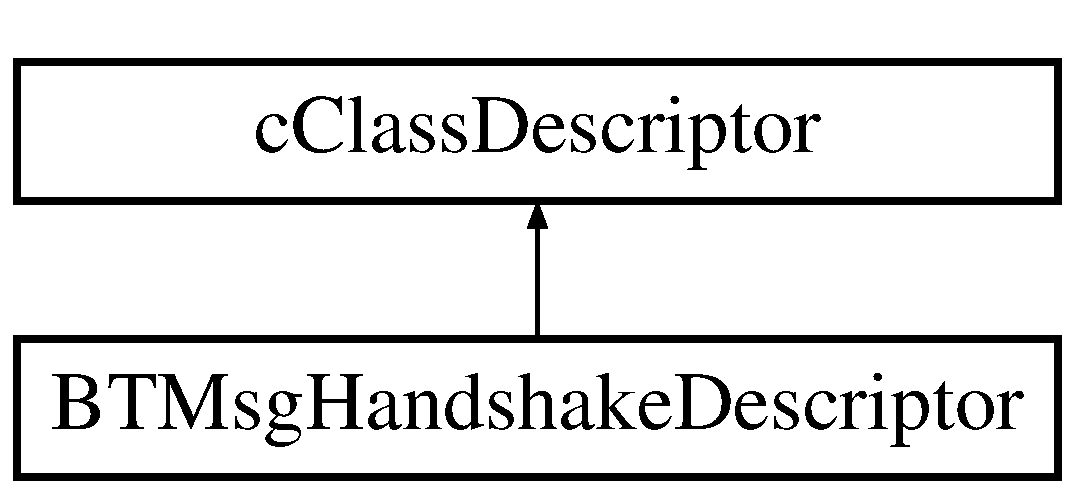
\includegraphics[height=2.000000cm]{classBTMsgHandshakeDescriptor}
\end{center}
\end{figure}
\subsection*{Public Member Functions}
\begin{DoxyCompactItemize}
\item 
\hyperlink{classBTMsgHandshakeDescriptor_a5fda9a4a966ab4efea32f0a8ecf2ef0b}{B\+T\+Msg\+Handshake\+Descriptor} ()
\item 
virtual \hyperlink{classBTMsgHandshakeDescriptor_a37bfa90eaff226afb84bd0a7edf602fc}{$\sim$\+B\+T\+Msg\+Handshake\+Descriptor} ()
\item 
virtual bool \hyperlink{classBTMsgHandshakeDescriptor_a26459f2666aa12b086978673336cdf76}{does\+Support} (c\+Object $\ast$obj) const 
\item 
virtual const char $\ast$ \hyperlink{classBTMsgHandshakeDescriptor_a90345d1a7dda62b8283e95171ffe5214}{get\+Property} (const char $\ast$propertyname) const 
\item 
virtual int \hyperlink{classBTMsgHandshakeDescriptor_a2e13fe51475fc4605a8f4644cf31b9ca}{get\+Field\+Count} (void $\ast$object) const 
\item 
virtual const char $\ast$ \hyperlink{classBTMsgHandshakeDescriptor_a9719d0cde93050068881a2cd97e7c09d}{get\+Field\+Name} (void $\ast$object, int field) const 
\item 
virtual int \hyperlink{classBTMsgHandshakeDescriptor_a4696f87e1ce1d592b5032d4206730c07}{find\+Field} (void $\ast$object, const char $\ast$field\+Name) const 
\item 
virtual unsigned int \hyperlink{classBTMsgHandshakeDescriptor_af550d1b7e2bdb09cf3028757c74f3708}{get\+Field\+Type\+Flags} (void $\ast$object, int field) const 
\item 
virtual const char $\ast$ \hyperlink{classBTMsgHandshakeDescriptor_a14410ec69bf59de282de47956ac822fa}{get\+Field\+Type\+String} (void $\ast$object, int field) const 
\item 
virtual const char $\ast$ \hyperlink{classBTMsgHandshakeDescriptor_a53f586d34e2be99aec32eb0408ba3441}{get\+Field\+Property} (void $\ast$object, int field, const char $\ast$propertyname) const 
\item 
virtual int \hyperlink{classBTMsgHandshakeDescriptor_a1c6aa2247d7fa5a3d07d77fc0f0e6c76}{get\+Array\+Size} (void $\ast$object, int field) const 
\item 
virtual std\+::string \hyperlink{classBTMsgHandshakeDescriptor_a409e1dd2baf1ccc2239b5f4a6d385832}{get\+Field\+As\+String} (void $\ast$object, int field, int i) const 
\item 
virtual bool \hyperlink{classBTMsgHandshakeDescriptor_a393af881d6a45d6d4e6cde5a11c87441}{set\+Field\+As\+String} (void $\ast$object, int field, int i, const char $\ast$value) const 
\item 
virtual const char $\ast$ \hyperlink{classBTMsgHandshakeDescriptor_a7c6b03870fa00006d365bce1ac91b951}{get\+Field\+Struct\+Name} (void $\ast$object, int field) const 
\item 
virtual void $\ast$ \hyperlink{classBTMsgHandshakeDescriptor_a8df09501d79546899dec28cd46c2dd70}{get\+Field\+Struct\+Pointer} (void $\ast$object, int field, int i) const 
\end{DoxyCompactItemize}


\subsection{Constructor \& Destructor Documentation}
\hypertarget{classBTMsgHandshakeDescriptor_a5fda9a4a966ab4efea32f0a8ecf2ef0b}{}\index{B\+T\+Msg\+Handshake\+Descriptor@{B\+T\+Msg\+Handshake\+Descriptor}!B\+T\+Msg\+Handshake\+Descriptor@{B\+T\+Msg\+Handshake\+Descriptor}}
\index{B\+T\+Msg\+Handshake\+Descriptor@{B\+T\+Msg\+Handshake\+Descriptor}!B\+T\+Msg\+Handshake\+Descriptor@{B\+T\+Msg\+Handshake\+Descriptor}}
\subsubsection[{B\+T\+Msg\+Handshake\+Descriptor()}]{\setlength{\rightskip}{0pt plus 5cm}B\+T\+Msg\+Handshake\+Descriptor\+::\+B\+T\+Msg\+Handshake\+Descriptor (
\begin{DoxyParamCaption}
{}
\end{DoxyParamCaption}
)}\label{classBTMsgHandshakeDescriptor_a5fda9a4a966ab4efea32f0a8ecf2ef0b}
\hypertarget{classBTMsgHandshakeDescriptor_a37bfa90eaff226afb84bd0a7edf602fc}{}\index{B\+T\+Msg\+Handshake\+Descriptor@{B\+T\+Msg\+Handshake\+Descriptor}!````~B\+T\+Msg\+Handshake\+Descriptor@{$\sim$\+B\+T\+Msg\+Handshake\+Descriptor}}
\index{````~B\+T\+Msg\+Handshake\+Descriptor@{$\sim$\+B\+T\+Msg\+Handshake\+Descriptor}!B\+T\+Msg\+Handshake\+Descriptor@{B\+T\+Msg\+Handshake\+Descriptor}}
\subsubsection[{$\sim$\+B\+T\+Msg\+Handshake\+Descriptor()}]{\setlength{\rightskip}{0pt plus 5cm}B\+T\+Msg\+Handshake\+Descriptor\+::$\sim$\+B\+T\+Msg\+Handshake\+Descriptor (
\begin{DoxyParamCaption}
{}
\end{DoxyParamCaption}
)\hspace{0.3cm}{\ttfamily [virtual]}}\label{classBTMsgHandshakeDescriptor_a37bfa90eaff226afb84bd0a7edf602fc}


\subsection{Member Function Documentation}
\hypertarget{classBTMsgHandshakeDescriptor_a26459f2666aa12b086978673336cdf76}{}\index{B\+T\+Msg\+Handshake\+Descriptor@{B\+T\+Msg\+Handshake\+Descriptor}!does\+Support@{does\+Support}}
\index{does\+Support@{does\+Support}!B\+T\+Msg\+Handshake\+Descriptor@{B\+T\+Msg\+Handshake\+Descriptor}}
\subsubsection[{does\+Support(c\+Object $\ast$obj) const }]{\setlength{\rightskip}{0pt plus 5cm}bool B\+T\+Msg\+Handshake\+Descriptor\+::does\+Support (
\begin{DoxyParamCaption}
\item[{c\+Object $\ast$}]{obj}
\end{DoxyParamCaption}
) const\hspace{0.3cm}{\ttfamily [virtual]}}\label{classBTMsgHandshakeDescriptor_a26459f2666aa12b086978673336cdf76}
\hypertarget{classBTMsgHandshakeDescriptor_a4696f87e1ce1d592b5032d4206730c07}{}\index{B\+T\+Msg\+Handshake\+Descriptor@{B\+T\+Msg\+Handshake\+Descriptor}!find\+Field@{find\+Field}}
\index{find\+Field@{find\+Field}!B\+T\+Msg\+Handshake\+Descriptor@{B\+T\+Msg\+Handshake\+Descriptor}}
\subsubsection[{find\+Field(void $\ast$object, const char $\ast$field\+Name) const }]{\setlength{\rightskip}{0pt plus 5cm}int B\+T\+Msg\+Handshake\+Descriptor\+::find\+Field (
\begin{DoxyParamCaption}
\item[{void $\ast$}]{object, }
\item[{const char $\ast$}]{field\+Name}
\end{DoxyParamCaption}
) const\hspace{0.3cm}{\ttfamily [virtual]}}\label{classBTMsgHandshakeDescriptor_a4696f87e1ce1d592b5032d4206730c07}
\hypertarget{classBTMsgHandshakeDescriptor_a1c6aa2247d7fa5a3d07d77fc0f0e6c76}{}\index{B\+T\+Msg\+Handshake\+Descriptor@{B\+T\+Msg\+Handshake\+Descriptor}!get\+Array\+Size@{get\+Array\+Size}}
\index{get\+Array\+Size@{get\+Array\+Size}!B\+T\+Msg\+Handshake\+Descriptor@{B\+T\+Msg\+Handshake\+Descriptor}}
\subsubsection[{get\+Array\+Size(void $\ast$object, int field) const }]{\setlength{\rightskip}{0pt plus 5cm}int B\+T\+Msg\+Handshake\+Descriptor\+::get\+Array\+Size (
\begin{DoxyParamCaption}
\item[{void $\ast$}]{object, }
\item[{int}]{field}
\end{DoxyParamCaption}
) const\hspace{0.3cm}{\ttfamily [virtual]}}\label{classBTMsgHandshakeDescriptor_a1c6aa2247d7fa5a3d07d77fc0f0e6c76}
\hypertarget{classBTMsgHandshakeDescriptor_a409e1dd2baf1ccc2239b5f4a6d385832}{}\index{B\+T\+Msg\+Handshake\+Descriptor@{B\+T\+Msg\+Handshake\+Descriptor}!get\+Field\+As\+String@{get\+Field\+As\+String}}
\index{get\+Field\+As\+String@{get\+Field\+As\+String}!B\+T\+Msg\+Handshake\+Descriptor@{B\+T\+Msg\+Handshake\+Descriptor}}
\subsubsection[{get\+Field\+As\+String(void $\ast$object, int field, int i) const }]{\setlength{\rightskip}{0pt plus 5cm}std\+::string B\+T\+Msg\+Handshake\+Descriptor\+::get\+Field\+As\+String (
\begin{DoxyParamCaption}
\item[{void $\ast$}]{object, }
\item[{int}]{field, }
\item[{int}]{i}
\end{DoxyParamCaption}
) const\hspace{0.3cm}{\ttfamily [virtual]}}\label{classBTMsgHandshakeDescriptor_a409e1dd2baf1ccc2239b5f4a6d385832}
\hypertarget{classBTMsgHandshakeDescriptor_a2e13fe51475fc4605a8f4644cf31b9ca}{}\index{B\+T\+Msg\+Handshake\+Descriptor@{B\+T\+Msg\+Handshake\+Descriptor}!get\+Field\+Count@{get\+Field\+Count}}
\index{get\+Field\+Count@{get\+Field\+Count}!B\+T\+Msg\+Handshake\+Descriptor@{B\+T\+Msg\+Handshake\+Descriptor}}
\subsubsection[{get\+Field\+Count(void $\ast$object) const }]{\setlength{\rightskip}{0pt plus 5cm}int B\+T\+Msg\+Handshake\+Descriptor\+::get\+Field\+Count (
\begin{DoxyParamCaption}
\item[{void $\ast$}]{object}
\end{DoxyParamCaption}
) const\hspace{0.3cm}{\ttfamily [virtual]}}\label{classBTMsgHandshakeDescriptor_a2e13fe51475fc4605a8f4644cf31b9ca}
\hypertarget{classBTMsgHandshakeDescriptor_a9719d0cde93050068881a2cd97e7c09d}{}\index{B\+T\+Msg\+Handshake\+Descriptor@{B\+T\+Msg\+Handshake\+Descriptor}!get\+Field\+Name@{get\+Field\+Name}}
\index{get\+Field\+Name@{get\+Field\+Name}!B\+T\+Msg\+Handshake\+Descriptor@{B\+T\+Msg\+Handshake\+Descriptor}}
\subsubsection[{get\+Field\+Name(void $\ast$object, int field) const }]{\setlength{\rightskip}{0pt plus 5cm}const char $\ast$ B\+T\+Msg\+Handshake\+Descriptor\+::get\+Field\+Name (
\begin{DoxyParamCaption}
\item[{void $\ast$}]{object, }
\item[{int}]{field}
\end{DoxyParamCaption}
) const\hspace{0.3cm}{\ttfamily [virtual]}}\label{classBTMsgHandshakeDescriptor_a9719d0cde93050068881a2cd97e7c09d}
\hypertarget{classBTMsgHandshakeDescriptor_a53f586d34e2be99aec32eb0408ba3441}{}\index{B\+T\+Msg\+Handshake\+Descriptor@{B\+T\+Msg\+Handshake\+Descriptor}!get\+Field\+Property@{get\+Field\+Property}}
\index{get\+Field\+Property@{get\+Field\+Property}!B\+T\+Msg\+Handshake\+Descriptor@{B\+T\+Msg\+Handshake\+Descriptor}}
\subsubsection[{get\+Field\+Property(void $\ast$object, int field, const char $\ast$propertyname) const }]{\setlength{\rightskip}{0pt plus 5cm}const char $\ast$ B\+T\+Msg\+Handshake\+Descriptor\+::get\+Field\+Property (
\begin{DoxyParamCaption}
\item[{void $\ast$}]{object, }
\item[{int}]{field, }
\item[{const char $\ast$}]{propertyname}
\end{DoxyParamCaption}
) const\hspace{0.3cm}{\ttfamily [virtual]}}\label{classBTMsgHandshakeDescriptor_a53f586d34e2be99aec32eb0408ba3441}
\hypertarget{classBTMsgHandshakeDescriptor_a7c6b03870fa00006d365bce1ac91b951}{}\index{B\+T\+Msg\+Handshake\+Descriptor@{B\+T\+Msg\+Handshake\+Descriptor}!get\+Field\+Struct\+Name@{get\+Field\+Struct\+Name}}
\index{get\+Field\+Struct\+Name@{get\+Field\+Struct\+Name}!B\+T\+Msg\+Handshake\+Descriptor@{B\+T\+Msg\+Handshake\+Descriptor}}
\subsubsection[{get\+Field\+Struct\+Name(void $\ast$object, int field) const }]{\setlength{\rightskip}{0pt plus 5cm}const char $\ast$ B\+T\+Msg\+Handshake\+Descriptor\+::get\+Field\+Struct\+Name (
\begin{DoxyParamCaption}
\item[{void $\ast$}]{object, }
\item[{int}]{field}
\end{DoxyParamCaption}
) const\hspace{0.3cm}{\ttfamily [virtual]}}\label{classBTMsgHandshakeDescriptor_a7c6b03870fa00006d365bce1ac91b951}
\hypertarget{classBTMsgHandshakeDescriptor_a8df09501d79546899dec28cd46c2dd70}{}\index{B\+T\+Msg\+Handshake\+Descriptor@{B\+T\+Msg\+Handshake\+Descriptor}!get\+Field\+Struct\+Pointer@{get\+Field\+Struct\+Pointer}}
\index{get\+Field\+Struct\+Pointer@{get\+Field\+Struct\+Pointer}!B\+T\+Msg\+Handshake\+Descriptor@{B\+T\+Msg\+Handshake\+Descriptor}}
\subsubsection[{get\+Field\+Struct\+Pointer(void $\ast$object, int field, int i) const }]{\setlength{\rightskip}{0pt plus 5cm}void $\ast$ B\+T\+Msg\+Handshake\+Descriptor\+::get\+Field\+Struct\+Pointer (
\begin{DoxyParamCaption}
\item[{void $\ast$}]{object, }
\item[{int}]{field, }
\item[{int}]{i}
\end{DoxyParamCaption}
) const\hspace{0.3cm}{\ttfamily [virtual]}}\label{classBTMsgHandshakeDescriptor_a8df09501d79546899dec28cd46c2dd70}
\hypertarget{classBTMsgHandshakeDescriptor_af550d1b7e2bdb09cf3028757c74f3708}{}\index{B\+T\+Msg\+Handshake\+Descriptor@{B\+T\+Msg\+Handshake\+Descriptor}!get\+Field\+Type\+Flags@{get\+Field\+Type\+Flags}}
\index{get\+Field\+Type\+Flags@{get\+Field\+Type\+Flags}!B\+T\+Msg\+Handshake\+Descriptor@{B\+T\+Msg\+Handshake\+Descriptor}}
\subsubsection[{get\+Field\+Type\+Flags(void $\ast$object, int field) const }]{\setlength{\rightskip}{0pt plus 5cm}unsigned int B\+T\+Msg\+Handshake\+Descriptor\+::get\+Field\+Type\+Flags (
\begin{DoxyParamCaption}
\item[{void $\ast$}]{object, }
\item[{int}]{field}
\end{DoxyParamCaption}
) const\hspace{0.3cm}{\ttfamily [virtual]}}\label{classBTMsgHandshakeDescriptor_af550d1b7e2bdb09cf3028757c74f3708}
\hypertarget{classBTMsgHandshakeDescriptor_a14410ec69bf59de282de47956ac822fa}{}\index{B\+T\+Msg\+Handshake\+Descriptor@{B\+T\+Msg\+Handshake\+Descriptor}!get\+Field\+Type\+String@{get\+Field\+Type\+String}}
\index{get\+Field\+Type\+String@{get\+Field\+Type\+String}!B\+T\+Msg\+Handshake\+Descriptor@{B\+T\+Msg\+Handshake\+Descriptor}}
\subsubsection[{get\+Field\+Type\+String(void $\ast$object, int field) const }]{\setlength{\rightskip}{0pt plus 5cm}const char $\ast$ B\+T\+Msg\+Handshake\+Descriptor\+::get\+Field\+Type\+String (
\begin{DoxyParamCaption}
\item[{void $\ast$}]{object, }
\item[{int}]{field}
\end{DoxyParamCaption}
) const\hspace{0.3cm}{\ttfamily [virtual]}}\label{classBTMsgHandshakeDescriptor_a14410ec69bf59de282de47956ac822fa}
\hypertarget{classBTMsgHandshakeDescriptor_a90345d1a7dda62b8283e95171ffe5214}{}\index{B\+T\+Msg\+Handshake\+Descriptor@{B\+T\+Msg\+Handshake\+Descriptor}!get\+Property@{get\+Property}}
\index{get\+Property@{get\+Property}!B\+T\+Msg\+Handshake\+Descriptor@{B\+T\+Msg\+Handshake\+Descriptor}}
\subsubsection[{get\+Property(const char $\ast$propertyname) const }]{\setlength{\rightskip}{0pt plus 5cm}const char $\ast$ B\+T\+Msg\+Handshake\+Descriptor\+::get\+Property (
\begin{DoxyParamCaption}
\item[{const char $\ast$}]{propertyname}
\end{DoxyParamCaption}
) const\hspace{0.3cm}{\ttfamily [virtual]}}\label{classBTMsgHandshakeDescriptor_a90345d1a7dda62b8283e95171ffe5214}
\hypertarget{classBTMsgHandshakeDescriptor_a393af881d6a45d6d4e6cde5a11c87441}{}\index{B\+T\+Msg\+Handshake\+Descriptor@{B\+T\+Msg\+Handshake\+Descriptor}!set\+Field\+As\+String@{set\+Field\+As\+String}}
\index{set\+Field\+As\+String@{set\+Field\+As\+String}!B\+T\+Msg\+Handshake\+Descriptor@{B\+T\+Msg\+Handshake\+Descriptor}}
\subsubsection[{set\+Field\+As\+String(void $\ast$object, int field, int i, const char $\ast$value) const }]{\setlength{\rightskip}{0pt plus 5cm}bool B\+T\+Msg\+Handshake\+Descriptor\+::set\+Field\+As\+String (
\begin{DoxyParamCaption}
\item[{void $\ast$}]{object, }
\item[{int}]{field, }
\item[{int}]{i, }
\item[{const char $\ast$}]{value}
\end{DoxyParamCaption}
) const\hspace{0.3cm}{\ttfamily [virtual]}}\label{classBTMsgHandshakeDescriptor_a393af881d6a45d6d4e6cde5a11c87441}


The documentation for this class was generated from the following file\+:\begin{DoxyCompactItemize}
\item 
\hyperlink{BTPeerWireMsg__m_8cc}{B\+T\+Peer\+Wire\+Msg\+\_\+m.\+cc}\end{DoxyCompactItemize}

\hypertarget{classBTPeerStateMsg}{}\section{B\+T\+Peer\+State\+Msg Class Reference}
\label{classBTPeerStateMsg}\index{B\+T\+Peer\+State\+Msg@{B\+T\+Peer\+State\+Msg}}


{\ttfamily \#include $<$B\+T\+Peer\+Wire\+Msg\+\_\+m.\+h$>$}

Inheritance diagram for B\+T\+Peer\+State\+Msg\+:\begin{figure}[H]
\begin{center}
\leavevmode
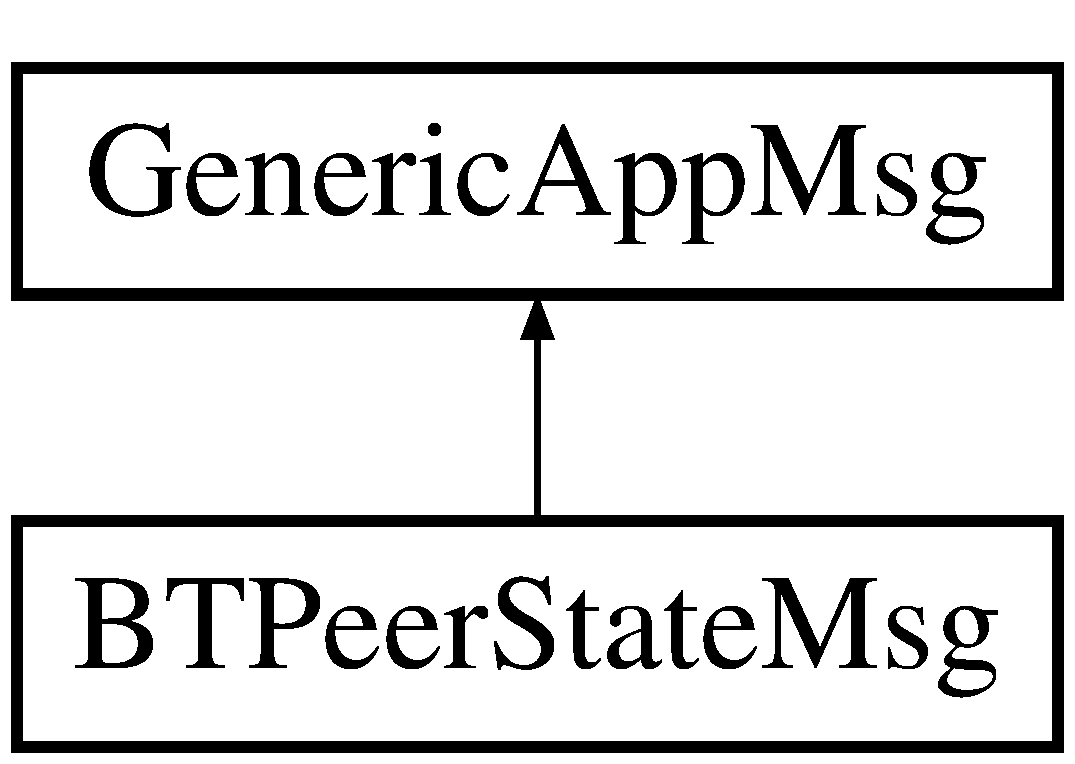
\includegraphics[height=2.000000cm]{classBTPeerStateMsg}
\end{center}
\end{figure}
\subsection*{Public Member Functions}
\begin{DoxyCompactItemize}
\item 
\hyperlink{classBTPeerStateMsg_ab7d14b0f1d4efff5a78abd8b6a1d857d}{B\+T\+Peer\+State\+Msg} (const char $\ast$name=N\+U\+L\+L, int kind=0)
\item 
\hyperlink{classBTPeerStateMsg_a5c60767152d203f9c1b539fb1e6ca7cf}{B\+T\+Peer\+State\+Msg} (const \hyperlink{classBTPeerStateMsg}{B\+T\+Peer\+State\+Msg} \&other)
\item 
virtual \hyperlink{classBTPeerStateMsg_aadb697d2f314297b44ce4b99b9ef01c9}{$\sim$\+B\+T\+Peer\+State\+Msg} ()
\item 
\hyperlink{classBTPeerStateMsg}{B\+T\+Peer\+State\+Msg} \& \hyperlink{classBTPeerStateMsg_add8adb86d08e11cb1a836c8374a03503}{operator=} (const \hyperlink{classBTPeerStateMsg}{B\+T\+Peer\+State\+Msg} \&other)
\item 
virtual \hyperlink{classBTPeerStateMsg}{B\+T\+Peer\+State\+Msg} $\ast$ \hyperlink{classBTPeerStateMsg_a73cc28ed5a32f0f89c43de5513549460}{dup} () const 
\item 
virtual void \hyperlink{classBTPeerStateMsg_ad7476812a0163cb9e40a2a5aaf3e4c81}{parsim\+Pack} (c\+Comm\+Buffer $\ast$b)
\item 
virtual void \hyperlink{classBTPeerStateMsg_a41a706a3d36a9ad449bd7a0e260c7ca3}{parsim\+Unpack} (c\+Comm\+Buffer $\ast$b)
\item 
virtual int \hyperlink{classBTPeerStateMsg_a06b4c4e77f189574c6938358c2195ed7}{length\+\_\+prefix} () const 
\item 
virtual void \hyperlink{classBTPeerStateMsg_a581d8941765c73c6381c8222011bbfe9}{set\+Length\+\_\+prefix} (int \hyperlink{classBTPeerStateMsg_ade7e3e6dbe30b3bdd9e796215e6a1ec6}{length\+\_\+prefix\+\_\+var})
\item 
virtual unsigned short \hyperlink{classBTPeerStateMsg_aa9c6f9b590d1d509d2338c9e18793331}{I\+D} () const 
\item 
virtual void \hyperlink{classBTPeerStateMsg_ac577434d76afb18476583b018a7c04d5}{set\+I\+D} (unsigned short \hyperlink{classBTPeerStateMsg_a10914bbd68aee3cf35b7a1718c7a0e9d}{I\+D\+\_\+var})
\end{DoxyCompactItemize}
\subsection*{Protected Member Functions}
\begin{DoxyCompactItemize}
\item 
bool \hyperlink{classBTPeerStateMsg_a58637665e79ee29402f85af914d16ffb}{operator==} (const \hyperlink{classBTPeerStateMsg}{B\+T\+Peer\+State\+Msg} \&)
\end{DoxyCompactItemize}
\subsection*{Protected Attributes}
\begin{DoxyCompactItemize}
\item 
int \hyperlink{classBTPeerStateMsg_ade7e3e6dbe30b3bdd9e796215e6a1ec6}{length\+\_\+prefix\+\_\+var}
\item 
unsigned short \hyperlink{classBTPeerStateMsg_a10914bbd68aee3cf35b7a1718c7a0e9d}{I\+D\+\_\+var}
\end{DoxyCompactItemize}


\subsection{Constructor \& Destructor Documentation}
\hypertarget{classBTPeerStateMsg_ab7d14b0f1d4efff5a78abd8b6a1d857d}{}\index{B\+T\+Peer\+State\+Msg@{B\+T\+Peer\+State\+Msg}!B\+T\+Peer\+State\+Msg@{B\+T\+Peer\+State\+Msg}}
\index{B\+T\+Peer\+State\+Msg@{B\+T\+Peer\+State\+Msg}!B\+T\+Peer\+State\+Msg@{B\+T\+Peer\+State\+Msg}}
\subsubsection[{B\+T\+Peer\+State\+Msg(const char $\ast$name=\+N\+U\+L\+L, int kind=0)}]{\setlength{\rightskip}{0pt plus 5cm}B\+T\+Peer\+State\+Msg\+::\+B\+T\+Peer\+State\+Msg (
\begin{DoxyParamCaption}
\item[{const char $\ast$}]{name = {\ttfamily NULL}, }
\item[{int}]{kind = {\ttfamily 0}}
\end{DoxyParamCaption}
)}\label{classBTPeerStateMsg_ab7d14b0f1d4efff5a78abd8b6a1d857d}
\hypertarget{classBTPeerStateMsg_a5c60767152d203f9c1b539fb1e6ca7cf}{}\index{B\+T\+Peer\+State\+Msg@{B\+T\+Peer\+State\+Msg}!B\+T\+Peer\+State\+Msg@{B\+T\+Peer\+State\+Msg}}
\index{B\+T\+Peer\+State\+Msg@{B\+T\+Peer\+State\+Msg}!B\+T\+Peer\+State\+Msg@{B\+T\+Peer\+State\+Msg}}
\subsubsection[{B\+T\+Peer\+State\+Msg(const B\+T\+Peer\+State\+Msg \&other)}]{\setlength{\rightskip}{0pt plus 5cm}B\+T\+Peer\+State\+Msg\+::\+B\+T\+Peer\+State\+Msg (
\begin{DoxyParamCaption}
\item[{const {\bf B\+T\+Peer\+State\+Msg} \&}]{other}
\end{DoxyParamCaption}
)}\label{classBTPeerStateMsg_a5c60767152d203f9c1b539fb1e6ca7cf}
\hypertarget{classBTPeerStateMsg_aadb697d2f314297b44ce4b99b9ef01c9}{}\index{B\+T\+Peer\+State\+Msg@{B\+T\+Peer\+State\+Msg}!````~B\+T\+Peer\+State\+Msg@{$\sim$\+B\+T\+Peer\+State\+Msg}}
\index{````~B\+T\+Peer\+State\+Msg@{$\sim$\+B\+T\+Peer\+State\+Msg}!B\+T\+Peer\+State\+Msg@{B\+T\+Peer\+State\+Msg}}
\subsubsection[{$\sim$\+B\+T\+Peer\+State\+Msg()}]{\setlength{\rightskip}{0pt plus 5cm}B\+T\+Peer\+State\+Msg\+::$\sim$\+B\+T\+Peer\+State\+Msg (
\begin{DoxyParamCaption}
{}
\end{DoxyParamCaption}
)\hspace{0.3cm}{\ttfamily [virtual]}}\label{classBTPeerStateMsg_aadb697d2f314297b44ce4b99b9ef01c9}


\subsection{Member Function Documentation}
\hypertarget{classBTPeerStateMsg_a73cc28ed5a32f0f89c43de5513549460}{}\index{B\+T\+Peer\+State\+Msg@{B\+T\+Peer\+State\+Msg}!dup@{dup}}
\index{dup@{dup}!B\+T\+Peer\+State\+Msg@{B\+T\+Peer\+State\+Msg}}
\subsubsection[{dup() const }]{\setlength{\rightskip}{0pt plus 5cm}virtual {\bf B\+T\+Peer\+State\+Msg}$\ast$ B\+T\+Peer\+State\+Msg\+::dup (
\begin{DoxyParamCaption}
{}
\end{DoxyParamCaption}
) const\hspace{0.3cm}{\ttfamily [inline]}, {\ttfamily [virtual]}}\label{classBTPeerStateMsg_a73cc28ed5a32f0f89c43de5513549460}
\hypertarget{classBTPeerStateMsg_aa9c6f9b590d1d509d2338c9e18793331}{}\index{B\+T\+Peer\+State\+Msg@{B\+T\+Peer\+State\+Msg}!I\+D@{I\+D}}
\index{I\+D@{I\+D}!B\+T\+Peer\+State\+Msg@{B\+T\+Peer\+State\+Msg}}
\subsubsection[{I\+D() const }]{\setlength{\rightskip}{0pt plus 5cm}unsigned short B\+T\+Peer\+State\+Msg\+::\+I\+D (
\begin{DoxyParamCaption}
{}
\end{DoxyParamCaption}
) const\hspace{0.3cm}{\ttfamily [virtual]}}\label{classBTPeerStateMsg_aa9c6f9b590d1d509d2338c9e18793331}
\hypertarget{classBTPeerStateMsg_a06b4c4e77f189574c6938358c2195ed7}{}\index{B\+T\+Peer\+State\+Msg@{B\+T\+Peer\+State\+Msg}!length\+\_\+prefix@{length\+\_\+prefix}}
\index{length\+\_\+prefix@{length\+\_\+prefix}!B\+T\+Peer\+State\+Msg@{B\+T\+Peer\+State\+Msg}}
\subsubsection[{length\+\_\+prefix() const }]{\setlength{\rightskip}{0pt plus 5cm}int B\+T\+Peer\+State\+Msg\+::length\+\_\+prefix (
\begin{DoxyParamCaption}
{}
\end{DoxyParamCaption}
) const\hspace{0.3cm}{\ttfamily [virtual]}}\label{classBTPeerStateMsg_a06b4c4e77f189574c6938358c2195ed7}
\hypertarget{classBTPeerStateMsg_add8adb86d08e11cb1a836c8374a03503}{}\index{B\+T\+Peer\+State\+Msg@{B\+T\+Peer\+State\+Msg}!operator=@{operator=}}
\index{operator=@{operator=}!B\+T\+Peer\+State\+Msg@{B\+T\+Peer\+State\+Msg}}
\subsubsection[{operator=(const B\+T\+Peer\+State\+Msg \&other)}]{\setlength{\rightskip}{0pt plus 5cm}{\bf B\+T\+Peer\+State\+Msg} \& B\+T\+Peer\+State\+Msg\+::operator= (
\begin{DoxyParamCaption}
\item[{const {\bf B\+T\+Peer\+State\+Msg} \&}]{other}
\end{DoxyParamCaption}
)}\label{classBTPeerStateMsg_add8adb86d08e11cb1a836c8374a03503}
\hypertarget{classBTPeerStateMsg_a58637665e79ee29402f85af914d16ffb}{}\index{B\+T\+Peer\+State\+Msg@{B\+T\+Peer\+State\+Msg}!operator==@{operator==}}
\index{operator==@{operator==}!B\+T\+Peer\+State\+Msg@{B\+T\+Peer\+State\+Msg}}
\subsubsection[{operator==(const B\+T\+Peer\+State\+Msg \&)}]{\setlength{\rightskip}{0pt plus 5cm}bool B\+T\+Peer\+State\+Msg\+::operator== (
\begin{DoxyParamCaption}
\item[{const {\bf B\+T\+Peer\+State\+Msg} \&}]{}
\end{DoxyParamCaption}
)\hspace{0.3cm}{\ttfamily [protected]}}\label{classBTPeerStateMsg_a58637665e79ee29402f85af914d16ffb}
\hypertarget{classBTPeerStateMsg_ad7476812a0163cb9e40a2a5aaf3e4c81}{}\index{B\+T\+Peer\+State\+Msg@{B\+T\+Peer\+State\+Msg}!parsim\+Pack@{parsim\+Pack}}
\index{parsim\+Pack@{parsim\+Pack}!B\+T\+Peer\+State\+Msg@{B\+T\+Peer\+State\+Msg}}
\subsubsection[{parsim\+Pack(c\+Comm\+Buffer $\ast$b)}]{\setlength{\rightskip}{0pt plus 5cm}void B\+T\+Peer\+State\+Msg\+::parsim\+Pack (
\begin{DoxyParamCaption}
\item[{c\+Comm\+Buffer $\ast$}]{b}
\end{DoxyParamCaption}
)\hspace{0.3cm}{\ttfamily [virtual]}}\label{classBTPeerStateMsg_ad7476812a0163cb9e40a2a5aaf3e4c81}
\hypertarget{classBTPeerStateMsg_a41a706a3d36a9ad449bd7a0e260c7ca3}{}\index{B\+T\+Peer\+State\+Msg@{B\+T\+Peer\+State\+Msg}!parsim\+Unpack@{parsim\+Unpack}}
\index{parsim\+Unpack@{parsim\+Unpack}!B\+T\+Peer\+State\+Msg@{B\+T\+Peer\+State\+Msg}}
\subsubsection[{parsim\+Unpack(c\+Comm\+Buffer $\ast$b)}]{\setlength{\rightskip}{0pt plus 5cm}void B\+T\+Peer\+State\+Msg\+::parsim\+Unpack (
\begin{DoxyParamCaption}
\item[{c\+Comm\+Buffer $\ast$}]{b}
\end{DoxyParamCaption}
)\hspace{0.3cm}{\ttfamily [virtual]}}\label{classBTPeerStateMsg_a41a706a3d36a9ad449bd7a0e260c7ca3}
\hypertarget{classBTPeerStateMsg_ac577434d76afb18476583b018a7c04d5}{}\index{B\+T\+Peer\+State\+Msg@{B\+T\+Peer\+State\+Msg}!set\+I\+D@{set\+I\+D}}
\index{set\+I\+D@{set\+I\+D}!B\+T\+Peer\+State\+Msg@{B\+T\+Peer\+State\+Msg}}
\subsubsection[{set\+I\+D(unsigned short I\+D\+\_\+var)}]{\setlength{\rightskip}{0pt plus 5cm}void B\+T\+Peer\+State\+Msg\+::set\+I\+D (
\begin{DoxyParamCaption}
\item[{unsigned short}]{I\+D\+\_\+var}
\end{DoxyParamCaption}
)\hspace{0.3cm}{\ttfamily [virtual]}}\label{classBTPeerStateMsg_ac577434d76afb18476583b018a7c04d5}
\hypertarget{classBTPeerStateMsg_a581d8941765c73c6381c8222011bbfe9}{}\index{B\+T\+Peer\+State\+Msg@{B\+T\+Peer\+State\+Msg}!set\+Length\+\_\+prefix@{set\+Length\+\_\+prefix}}
\index{set\+Length\+\_\+prefix@{set\+Length\+\_\+prefix}!B\+T\+Peer\+State\+Msg@{B\+T\+Peer\+State\+Msg}}
\subsubsection[{set\+Length\+\_\+prefix(int length\+\_\+prefix\+\_\+var)}]{\setlength{\rightskip}{0pt plus 5cm}void B\+T\+Peer\+State\+Msg\+::set\+Length\+\_\+prefix (
\begin{DoxyParamCaption}
\item[{int}]{length\+\_\+prefix\+\_\+var}
\end{DoxyParamCaption}
)\hspace{0.3cm}{\ttfamily [virtual]}}\label{classBTPeerStateMsg_a581d8941765c73c6381c8222011bbfe9}


\subsection{Member Data Documentation}
\hypertarget{classBTPeerStateMsg_a10914bbd68aee3cf35b7a1718c7a0e9d}{}\index{B\+T\+Peer\+State\+Msg@{B\+T\+Peer\+State\+Msg}!I\+D\+\_\+var@{I\+D\+\_\+var}}
\index{I\+D\+\_\+var@{I\+D\+\_\+var}!B\+T\+Peer\+State\+Msg@{B\+T\+Peer\+State\+Msg}}
\subsubsection[{I\+D\+\_\+var}]{\setlength{\rightskip}{0pt plus 5cm}unsigned short B\+T\+Peer\+State\+Msg\+::\+I\+D\+\_\+var\hspace{0.3cm}{\ttfamily [protected]}}\label{classBTPeerStateMsg_a10914bbd68aee3cf35b7a1718c7a0e9d}
\hypertarget{classBTPeerStateMsg_ade7e3e6dbe30b3bdd9e796215e6a1ec6}{}\index{B\+T\+Peer\+State\+Msg@{B\+T\+Peer\+State\+Msg}!length\+\_\+prefix\+\_\+var@{length\+\_\+prefix\+\_\+var}}
\index{length\+\_\+prefix\+\_\+var@{length\+\_\+prefix\+\_\+var}!B\+T\+Peer\+State\+Msg@{B\+T\+Peer\+State\+Msg}}
\subsubsection[{length\+\_\+prefix\+\_\+var}]{\setlength{\rightskip}{0pt plus 5cm}int B\+T\+Peer\+State\+Msg\+::length\+\_\+prefix\+\_\+var\hspace{0.3cm}{\ttfamily [protected]}}\label{classBTPeerStateMsg_ade7e3e6dbe30b3bdd9e796215e6a1ec6}


The documentation for this class was generated from the following files\+:\begin{DoxyCompactItemize}
\item 
\hyperlink{BTPeerWireMsg__m_8h}{B\+T\+Peer\+Wire\+Msg\+\_\+m.\+h}\item 
\hyperlink{BTPeerWireMsg__m_8cc}{B\+T\+Peer\+Wire\+Msg\+\_\+m.\+cc}\end{DoxyCompactItemize}

\hypertarget{classBTPeerStateMsgDescriptor}{}\section{B\+T\+Peer\+State\+Msg\+Descriptor Class Reference}
\label{classBTPeerStateMsgDescriptor}\index{B\+T\+Peer\+State\+Msg\+Descriptor@{B\+T\+Peer\+State\+Msg\+Descriptor}}
Inheritance diagram for B\+T\+Peer\+State\+Msg\+Descriptor\+:\begin{figure}[H]
\begin{center}
\leavevmode
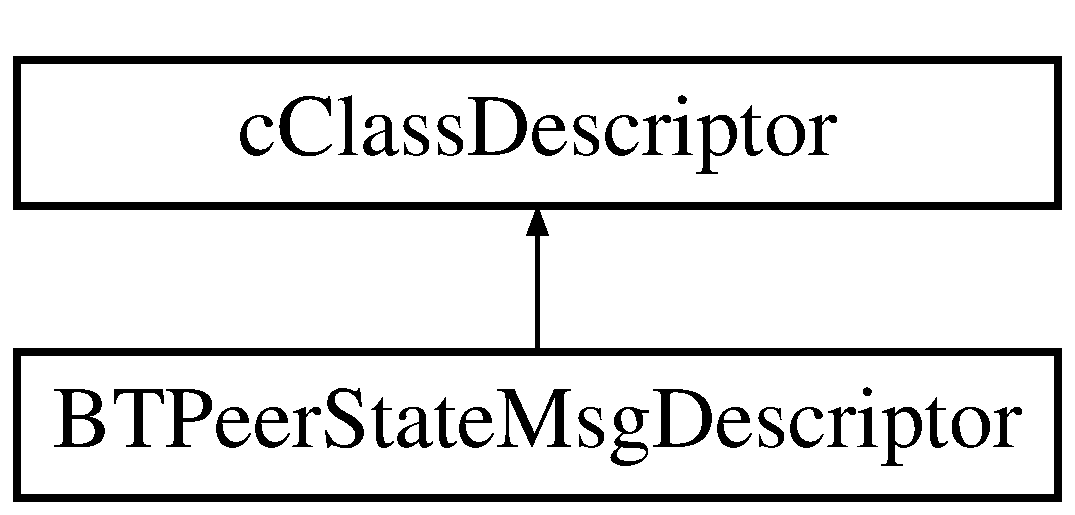
\includegraphics[height=2.000000cm]{classBTPeerStateMsgDescriptor}
\end{center}
\end{figure}
\subsection*{Public Member Functions}
\begin{DoxyCompactItemize}
\item 
\hyperlink{classBTPeerStateMsgDescriptor_afbe153c943bdbaf08267d18ef1eb3ddd}{B\+T\+Peer\+State\+Msg\+Descriptor} ()
\item 
virtual \hyperlink{classBTPeerStateMsgDescriptor_a9619e3d770a31134405918c8f8399e84}{$\sim$\+B\+T\+Peer\+State\+Msg\+Descriptor} ()
\item 
virtual bool \hyperlink{classBTPeerStateMsgDescriptor_a89df95af44ba98c8131ca509060ff2e3}{does\+Support} (c\+Object $\ast$obj) const 
\item 
virtual const char $\ast$ \hyperlink{classBTPeerStateMsgDescriptor_a3ce19be83bc8b95050ecf078ac961c3f}{get\+Property} (const char $\ast$propertyname) const 
\item 
virtual int \hyperlink{classBTPeerStateMsgDescriptor_a40478abf31c5ba0c98cb715ce4af408e}{get\+Field\+Count} (void $\ast$object) const 
\item 
virtual const char $\ast$ \hyperlink{classBTPeerStateMsgDescriptor_a8f46fdfec6da532f2dd8c007b929db70}{get\+Field\+Name} (void $\ast$object, int field) const 
\item 
virtual int \hyperlink{classBTPeerStateMsgDescriptor_a3612922faba9e40dd0c73a1eb13fc7c8}{find\+Field} (void $\ast$object, const char $\ast$field\+Name) const 
\item 
virtual unsigned int \hyperlink{classBTPeerStateMsgDescriptor_ab453e5665f0979b623681234370a2603}{get\+Field\+Type\+Flags} (void $\ast$object, int field) const 
\item 
virtual const char $\ast$ \hyperlink{classBTPeerStateMsgDescriptor_a0f767afb60b1a49a6c1ed5af51870b00}{get\+Field\+Type\+String} (void $\ast$object, int field) const 
\item 
virtual const char $\ast$ \hyperlink{classBTPeerStateMsgDescriptor_adc631362e3fdf1f7b0ad447330f1df5f}{get\+Field\+Property} (void $\ast$object, int field, const char $\ast$propertyname) const 
\item 
virtual int \hyperlink{classBTPeerStateMsgDescriptor_aec03fd31374edc82d8429080065c2c65}{get\+Array\+Size} (void $\ast$object, int field) const 
\item 
virtual std\+::string \hyperlink{classBTPeerStateMsgDescriptor_a1ca01f72efbc6d6a3f1ac47e0a635128}{get\+Field\+As\+String} (void $\ast$object, int field, int i) const 
\item 
virtual bool \hyperlink{classBTPeerStateMsgDescriptor_ab514b3e648369e13da78c6b9b61cfd9d}{set\+Field\+As\+String} (void $\ast$object, int field, int i, const char $\ast$value) const 
\item 
virtual const char $\ast$ \hyperlink{classBTPeerStateMsgDescriptor_add7dfead37803e22c30e8e0e8062c6b3}{get\+Field\+Struct\+Name} (void $\ast$object, int field) const 
\item 
virtual void $\ast$ \hyperlink{classBTPeerStateMsgDescriptor_ac339b448ba235abd44fc2f39bf4a6041}{get\+Field\+Struct\+Pointer} (void $\ast$object, int field, int i) const 
\end{DoxyCompactItemize}


\subsection{Constructor \& Destructor Documentation}
\hypertarget{classBTPeerStateMsgDescriptor_afbe153c943bdbaf08267d18ef1eb3ddd}{}\index{B\+T\+Peer\+State\+Msg\+Descriptor@{B\+T\+Peer\+State\+Msg\+Descriptor}!B\+T\+Peer\+State\+Msg\+Descriptor@{B\+T\+Peer\+State\+Msg\+Descriptor}}
\index{B\+T\+Peer\+State\+Msg\+Descriptor@{B\+T\+Peer\+State\+Msg\+Descriptor}!B\+T\+Peer\+State\+Msg\+Descriptor@{B\+T\+Peer\+State\+Msg\+Descriptor}}
\subsubsection[{B\+T\+Peer\+State\+Msg\+Descriptor()}]{\setlength{\rightskip}{0pt plus 5cm}B\+T\+Peer\+State\+Msg\+Descriptor\+::\+B\+T\+Peer\+State\+Msg\+Descriptor (
\begin{DoxyParamCaption}
{}
\end{DoxyParamCaption}
)}\label{classBTPeerStateMsgDescriptor_afbe153c943bdbaf08267d18ef1eb3ddd}
\hypertarget{classBTPeerStateMsgDescriptor_a9619e3d770a31134405918c8f8399e84}{}\index{B\+T\+Peer\+State\+Msg\+Descriptor@{B\+T\+Peer\+State\+Msg\+Descriptor}!````~B\+T\+Peer\+State\+Msg\+Descriptor@{$\sim$\+B\+T\+Peer\+State\+Msg\+Descriptor}}
\index{````~B\+T\+Peer\+State\+Msg\+Descriptor@{$\sim$\+B\+T\+Peer\+State\+Msg\+Descriptor}!B\+T\+Peer\+State\+Msg\+Descriptor@{B\+T\+Peer\+State\+Msg\+Descriptor}}
\subsubsection[{$\sim$\+B\+T\+Peer\+State\+Msg\+Descriptor()}]{\setlength{\rightskip}{0pt plus 5cm}B\+T\+Peer\+State\+Msg\+Descriptor\+::$\sim$\+B\+T\+Peer\+State\+Msg\+Descriptor (
\begin{DoxyParamCaption}
{}
\end{DoxyParamCaption}
)\hspace{0.3cm}{\ttfamily [virtual]}}\label{classBTPeerStateMsgDescriptor_a9619e3d770a31134405918c8f8399e84}


\subsection{Member Function Documentation}
\hypertarget{classBTPeerStateMsgDescriptor_a89df95af44ba98c8131ca509060ff2e3}{}\index{B\+T\+Peer\+State\+Msg\+Descriptor@{B\+T\+Peer\+State\+Msg\+Descriptor}!does\+Support@{does\+Support}}
\index{does\+Support@{does\+Support}!B\+T\+Peer\+State\+Msg\+Descriptor@{B\+T\+Peer\+State\+Msg\+Descriptor}}
\subsubsection[{does\+Support(c\+Object $\ast$obj) const }]{\setlength{\rightskip}{0pt plus 5cm}bool B\+T\+Peer\+State\+Msg\+Descriptor\+::does\+Support (
\begin{DoxyParamCaption}
\item[{c\+Object $\ast$}]{obj}
\end{DoxyParamCaption}
) const\hspace{0.3cm}{\ttfamily [virtual]}}\label{classBTPeerStateMsgDescriptor_a89df95af44ba98c8131ca509060ff2e3}
\hypertarget{classBTPeerStateMsgDescriptor_a3612922faba9e40dd0c73a1eb13fc7c8}{}\index{B\+T\+Peer\+State\+Msg\+Descriptor@{B\+T\+Peer\+State\+Msg\+Descriptor}!find\+Field@{find\+Field}}
\index{find\+Field@{find\+Field}!B\+T\+Peer\+State\+Msg\+Descriptor@{B\+T\+Peer\+State\+Msg\+Descriptor}}
\subsubsection[{find\+Field(void $\ast$object, const char $\ast$field\+Name) const }]{\setlength{\rightskip}{0pt plus 5cm}int B\+T\+Peer\+State\+Msg\+Descriptor\+::find\+Field (
\begin{DoxyParamCaption}
\item[{void $\ast$}]{object, }
\item[{const char $\ast$}]{field\+Name}
\end{DoxyParamCaption}
) const\hspace{0.3cm}{\ttfamily [virtual]}}\label{classBTPeerStateMsgDescriptor_a3612922faba9e40dd0c73a1eb13fc7c8}
\hypertarget{classBTPeerStateMsgDescriptor_aec03fd31374edc82d8429080065c2c65}{}\index{B\+T\+Peer\+State\+Msg\+Descriptor@{B\+T\+Peer\+State\+Msg\+Descriptor}!get\+Array\+Size@{get\+Array\+Size}}
\index{get\+Array\+Size@{get\+Array\+Size}!B\+T\+Peer\+State\+Msg\+Descriptor@{B\+T\+Peer\+State\+Msg\+Descriptor}}
\subsubsection[{get\+Array\+Size(void $\ast$object, int field) const }]{\setlength{\rightskip}{0pt plus 5cm}int B\+T\+Peer\+State\+Msg\+Descriptor\+::get\+Array\+Size (
\begin{DoxyParamCaption}
\item[{void $\ast$}]{object, }
\item[{int}]{field}
\end{DoxyParamCaption}
) const\hspace{0.3cm}{\ttfamily [virtual]}}\label{classBTPeerStateMsgDescriptor_aec03fd31374edc82d8429080065c2c65}
\hypertarget{classBTPeerStateMsgDescriptor_a1ca01f72efbc6d6a3f1ac47e0a635128}{}\index{B\+T\+Peer\+State\+Msg\+Descriptor@{B\+T\+Peer\+State\+Msg\+Descriptor}!get\+Field\+As\+String@{get\+Field\+As\+String}}
\index{get\+Field\+As\+String@{get\+Field\+As\+String}!B\+T\+Peer\+State\+Msg\+Descriptor@{B\+T\+Peer\+State\+Msg\+Descriptor}}
\subsubsection[{get\+Field\+As\+String(void $\ast$object, int field, int i) const }]{\setlength{\rightskip}{0pt plus 5cm}std\+::string B\+T\+Peer\+State\+Msg\+Descriptor\+::get\+Field\+As\+String (
\begin{DoxyParamCaption}
\item[{void $\ast$}]{object, }
\item[{int}]{field, }
\item[{int}]{i}
\end{DoxyParamCaption}
) const\hspace{0.3cm}{\ttfamily [virtual]}}\label{classBTPeerStateMsgDescriptor_a1ca01f72efbc6d6a3f1ac47e0a635128}
\hypertarget{classBTPeerStateMsgDescriptor_a40478abf31c5ba0c98cb715ce4af408e}{}\index{B\+T\+Peer\+State\+Msg\+Descriptor@{B\+T\+Peer\+State\+Msg\+Descriptor}!get\+Field\+Count@{get\+Field\+Count}}
\index{get\+Field\+Count@{get\+Field\+Count}!B\+T\+Peer\+State\+Msg\+Descriptor@{B\+T\+Peer\+State\+Msg\+Descriptor}}
\subsubsection[{get\+Field\+Count(void $\ast$object) const }]{\setlength{\rightskip}{0pt plus 5cm}int B\+T\+Peer\+State\+Msg\+Descriptor\+::get\+Field\+Count (
\begin{DoxyParamCaption}
\item[{void $\ast$}]{object}
\end{DoxyParamCaption}
) const\hspace{0.3cm}{\ttfamily [virtual]}}\label{classBTPeerStateMsgDescriptor_a40478abf31c5ba0c98cb715ce4af408e}
\hypertarget{classBTPeerStateMsgDescriptor_a8f46fdfec6da532f2dd8c007b929db70}{}\index{B\+T\+Peer\+State\+Msg\+Descriptor@{B\+T\+Peer\+State\+Msg\+Descriptor}!get\+Field\+Name@{get\+Field\+Name}}
\index{get\+Field\+Name@{get\+Field\+Name}!B\+T\+Peer\+State\+Msg\+Descriptor@{B\+T\+Peer\+State\+Msg\+Descriptor}}
\subsubsection[{get\+Field\+Name(void $\ast$object, int field) const }]{\setlength{\rightskip}{0pt plus 5cm}const char $\ast$ B\+T\+Peer\+State\+Msg\+Descriptor\+::get\+Field\+Name (
\begin{DoxyParamCaption}
\item[{void $\ast$}]{object, }
\item[{int}]{field}
\end{DoxyParamCaption}
) const\hspace{0.3cm}{\ttfamily [virtual]}}\label{classBTPeerStateMsgDescriptor_a8f46fdfec6da532f2dd8c007b929db70}
\hypertarget{classBTPeerStateMsgDescriptor_adc631362e3fdf1f7b0ad447330f1df5f}{}\index{B\+T\+Peer\+State\+Msg\+Descriptor@{B\+T\+Peer\+State\+Msg\+Descriptor}!get\+Field\+Property@{get\+Field\+Property}}
\index{get\+Field\+Property@{get\+Field\+Property}!B\+T\+Peer\+State\+Msg\+Descriptor@{B\+T\+Peer\+State\+Msg\+Descriptor}}
\subsubsection[{get\+Field\+Property(void $\ast$object, int field, const char $\ast$propertyname) const }]{\setlength{\rightskip}{0pt plus 5cm}const char $\ast$ B\+T\+Peer\+State\+Msg\+Descriptor\+::get\+Field\+Property (
\begin{DoxyParamCaption}
\item[{void $\ast$}]{object, }
\item[{int}]{field, }
\item[{const char $\ast$}]{propertyname}
\end{DoxyParamCaption}
) const\hspace{0.3cm}{\ttfamily [virtual]}}\label{classBTPeerStateMsgDescriptor_adc631362e3fdf1f7b0ad447330f1df5f}
\hypertarget{classBTPeerStateMsgDescriptor_add7dfead37803e22c30e8e0e8062c6b3}{}\index{B\+T\+Peer\+State\+Msg\+Descriptor@{B\+T\+Peer\+State\+Msg\+Descriptor}!get\+Field\+Struct\+Name@{get\+Field\+Struct\+Name}}
\index{get\+Field\+Struct\+Name@{get\+Field\+Struct\+Name}!B\+T\+Peer\+State\+Msg\+Descriptor@{B\+T\+Peer\+State\+Msg\+Descriptor}}
\subsubsection[{get\+Field\+Struct\+Name(void $\ast$object, int field) const }]{\setlength{\rightskip}{0pt plus 5cm}const char $\ast$ B\+T\+Peer\+State\+Msg\+Descriptor\+::get\+Field\+Struct\+Name (
\begin{DoxyParamCaption}
\item[{void $\ast$}]{object, }
\item[{int}]{field}
\end{DoxyParamCaption}
) const\hspace{0.3cm}{\ttfamily [virtual]}}\label{classBTPeerStateMsgDescriptor_add7dfead37803e22c30e8e0e8062c6b3}
\hypertarget{classBTPeerStateMsgDescriptor_ac339b448ba235abd44fc2f39bf4a6041}{}\index{B\+T\+Peer\+State\+Msg\+Descriptor@{B\+T\+Peer\+State\+Msg\+Descriptor}!get\+Field\+Struct\+Pointer@{get\+Field\+Struct\+Pointer}}
\index{get\+Field\+Struct\+Pointer@{get\+Field\+Struct\+Pointer}!B\+T\+Peer\+State\+Msg\+Descriptor@{B\+T\+Peer\+State\+Msg\+Descriptor}}
\subsubsection[{get\+Field\+Struct\+Pointer(void $\ast$object, int field, int i) const }]{\setlength{\rightskip}{0pt plus 5cm}void $\ast$ B\+T\+Peer\+State\+Msg\+Descriptor\+::get\+Field\+Struct\+Pointer (
\begin{DoxyParamCaption}
\item[{void $\ast$}]{object, }
\item[{int}]{field, }
\item[{int}]{i}
\end{DoxyParamCaption}
) const\hspace{0.3cm}{\ttfamily [virtual]}}\label{classBTPeerStateMsgDescriptor_ac339b448ba235abd44fc2f39bf4a6041}
\hypertarget{classBTPeerStateMsgDescriptor_ab453e5665f0979b623681234370a2603}{}\index{B\+T\+Peer\+State\+Msg\+Descriptor@{B\+T\+Peer\+State\+Msg\+Descriptor}!get\+Field\+Type\+Flags@{get\+Field\+Type\+Flags}}
\index{get\+Field\+Type\+Flags@{get\+Field\+Type\+Flags}!B\+T\+Peer\+State\+Msg\+Descriptor@{B\+T\+Peer\+State\+Msg\+Descriptor}}
\subsubsection[{get\+Field\+Type\+Flags(void $\ast$object, int field) const }]{\setlength{\rightskip}{0pt plus 5cm}unsigned int B\+T\+Peer\+State\+Msg\+Descriptor\+::get\+Field\+Type\+Flags (
\begin{DoxyParamCaption}
\item[{void $\ast$}]{object, }
\item[{int}]{field}
\end{DoxyParamCaption}
) const\hspace{0.3cm}{\ttfamily [virtual]}}\label{classBTPeerStateMsgDescriptor_ab453e5665f0979b623681234370a2603}
\hypertarget{classBTPeerStateMsgDescriptor_a0f767afb60b1a49a6c1ed5af51870b00}{}\index{B\+T\+Peer\+State\+Msg\+Descriptor@{B\+T\+Peer\+State\+Msg\+Descriptor}!get\+Field\+Type\+String@{get\+Field\+Type\+String}}
\index{get\+Field\+Type\+String@{get\+Field\+Type\+String}!B\+T\+Peer\+State\+Msg\+Descriptor@{B\+T\+Peer\+State\+Msg\+Descriptor}}
\subsubsection[{get\+Field\+Type\+String(void $\ast$object, int field) const }]{\setlength{\rightskip}{0pt plus 5cm}const char $\ast$ B\+T\+Peer\+State\+Msg\+Descriptor\+::get\+Field\+Type\+String (
\begin{DoxyParamCaption}
\item[{void $\ast$}]{object, }
\item[{int}]{field}
\end{DoxyParamCaption}
) const\hspace{0.3cm}{\ttfamily [virtual]}}\label{classBTPeerStateMsgDescriptor_a0f767afb60b1a49a6c1ed5af51870b00}
\hypertarget{classBTPeerStateMsgDescriptor_a3ce19be83bc8b95050ecf078ac961c3f}{}\index{B\+T\+Peer\+State\+Msg\+Descriptor@{B\+T\+Peer\+State\+Msg\+Descriptor}!get\+Property@{get\+Property}}
\index{get\+Property@{get\+Property}!B\+T\+Peer\+State\+Msg\+Descriptor@{B\+T\+Peer\+State\+Msg\+Descriptor}}
\subsubsection[{get\+Property(const char $\ast$propertyname) const }]{\setlength{\rightskip}{0pt plus 5cm}const char $\ast$ B\+T\+Peer\+State\+Msg\+Descriptor\+::get\+Property (
\begin{DoxyParamCaption}
\item[{const char $\ast$}]{propertyname}
\end{DoxyParamCaption}
) const\hspace{0.3cm}{\ttfamily [virtual]}}\label{classBTPeerStateMsgDescriptor_a3ce19be83bc8b95050ecf078ac961c3f}
\hypertarget{classBTPeerStateMsgDescriptor_ab514b3e648369e13da78c6b9b61cfd9d}{}\index{B\+T\+Peer\+State\+Msg\+Descriptor@{B\+T\+Peer\+State\+Msg\+Descriptor}!set\+Field\+As\+String@{set\+Field\+As\+String}}
\index{set\+Field\+As\+String@{set\+Field\+As\+String}!B\+T\+Peer\+State\+Msg\+Descriptor@{B\+T\+Peer\+State\+Msg\+Descriptor}}
\subsubsection[{set\+Field\+As\+String(void $\ast$object, int field, int i, const char $\ast$value) const }]{\setlength{\rightskip}{0pt plus 5cm}bool B\+T\+Peer\+State\+Msg\+Descriptor\+::set\+Field\+As\+String (
\begin{DoxyParamCaption}
\item[{void $\ast$}]{object, }
\item[{int}]{field, }
\item[{int}]{i, }
\item[{const char $\ast$}]{value}
\end{DoxyParamCaption}
) const\hspace{0.3cm}{\ttfamily [virtual]}}\label{classBTPeerStateMsgDescriptor_ab514b3e648369e13da78c6b9b61cfd9d}


The documentation for this class was generated from the following file\+:\begin{DoxyCompactItemize}
\item 
\hyperlink{BTPeerWireMsg__m_8cc}{B\+T\+Peer\+Wire\+Msg\+\_\+m.\+cc}\end{DoxyCompactItemize}

\hypertarget{classBTPeerWireBase}{}\section{B\+T\+Peer\+Wire\+Base Class Reference}
\label{classBTPeerWireBase}\index{B\+T\+Peer\+Wire\+Base@{B\+T\+Peer\+Wire\+Base}}


{\ttfamily \#include $<$B\+T\+Peer\+Wire\+Base.\+h$>$}

Inheritance diagram for B\+T\+Peer\+Wire\+Base\+:\begin{figure}[H]
\begin{center}
\leavevmode
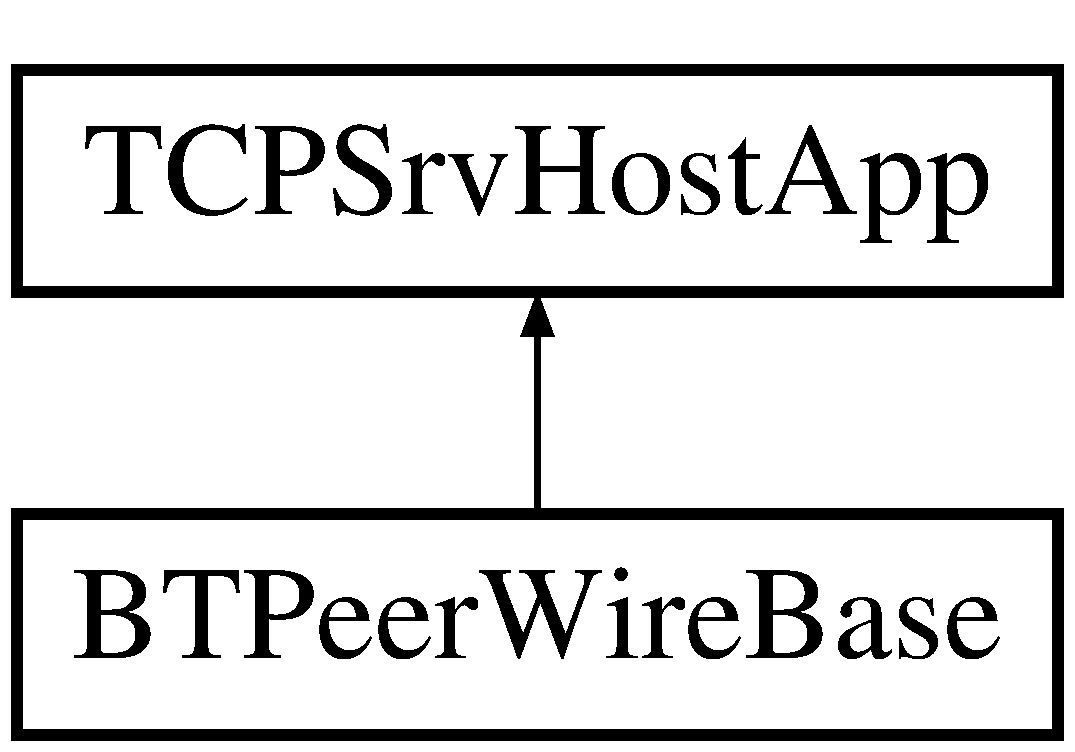
\includegraphics[height=2.000000cm]{classBTPeerWireBase}
\end{center}
\end{figure}
\subsection*{Public Member Functions}
\begin{DoxyCompactItemize}
\item 
\hyperlink{classBTPeerWireBase_ac0f4fe0fb674d693ec56e936b07ec9ce}{B\+T\+Peer\+Wire\+Base} ()
\item 
virtual \hyperlink{classBTPeerWireBase_a973e3484fdff1603e77aab6b8dc036b7}{$\sim$\+B\+T\+Peer\+Wire\+Base} ()
\item 
\hyperlink{classPeerState}{Peer\+State} \hyperlink{classBTPeerWireBase_aaece1bc1f54f78f704a6d8f122866ec8}{get\+Peer\+State} ()
\item 
double \hyperlink{classBTPeerWireBase_a5ba1f14a19dfbc488080c0fde88e1440}{file\+Size} ()
\item 
void \hyperlink{classBTPeerWireBase_a424ebf4ed4a42eb208939f198d7fb7f4}{set\+File\+Size} (double)
\item 
double \hyperlink{classBTPeerWireBase_ac66fc52cacb612adfa1314eb06610afe}{piece\+Size} ()
\item 
void \hyperlink{classBTPeerWireBase_a49e5078e88e79d72256f94b604503b2f}{set\+Piece\+Size} (double)
\item 
double \hyperlink{classBTPeerWireBase_a876a1131637f5db2ae216fe7ac19332a}{block\+Size} ()
\item 
void \hyperlink{classBTPeerWireBase_a070f6c47f701e48e7843f731ec07c1a4}{set\+Block\+Size} (double)
\item 
bool \hyperlink{classBTPeerWireBase_ad75a24948d3225218fdcba16a3b97152}{http\+Use} ()
\item 
void \hyperlink{classBTPeerWireBase_a80ba3561ebe152f11b19081e2193bbf0}{set\+Http\+Use} (bool)
\item 
bool \hyperlink{classBTPeerWireBase_aa06acdd860849b17b073c9eedffc5fab}{http\+Cache\+Use} ()
\item 
void \hyperlink{classBTPeerWireBase_ac1292272489b42e6c5e012247f05ad77}{set\+Http\+Cache\+Use} (bool)
\item 
T\+C\+P\+Server\+Thread\+Base $\ast$ \hyperlink{classBTPeerWireBase_a200ae42b2d1b1b107b6dc5de99da0dc7}{get\+Cache\+Thread} ()
\item 
int \hyperlink{classBTPeerWireBase_ac638e905388b0d4a3fdfba66d4e1a995}{D\+H\+T\+Port} ()
\item 
void \hyperlink{classBTPeerWireBase_a10bffb581df8f5365309cd74c780d9ad}{set\+D\+H\+T\+Port} (int)
\item 
const char $\ast$ \hyperlink{classBTPeerWireBase_aa7b0cc25e91a06b24f7b95574f0244cb}{pstr} ()
\item 
int \hyperlink{classBTPeerWireBase_a29176942239a5a4e8f6106cd0fc89bca}{pstrlen} ()
\item 
int \hyperlink{classBTPeerWireBase_a850b87f6cf6d6a0ade4895971ccef6f1}{keep\+Alive} ()
\item 
void \hyperlink{classBTPeerWireBase_ac7f31840e3d4b21046150178489115b0}{set\+Keep\+Alive} (int)
\item 
bool \hyperlink{classBTPeerWireBase_a06e9594abde1cb67ea5cad74334d9df5}{have\+Supression} ()
\item 
void \hyperlink{classBTPeerWireBase_a4daf47299e5700e78bb436d03fb28176}{set\+Have\+Supression} (bool)
\item 
int \hyperlink{classBTPeerWireBase_a38731ea77adc66c533c5ffdf122cec49}{chocking\+Interval} ()
\item 
void \hyperlink{classBTPeerWireBase_a12b80e9d6e09391fad908943db5b64d8}{set\+Chocking\+Interval} (int)
\item 
int \hyperlink{classBTPeerWireBase_a86978d47f64d7858603ac0427a2c20c6}{downloaders} ()
\item 
void \hyperlink{classBTPeerWireBase_ab93d18bc780a3990b06cc6eb979a7370}{set\+Downloaders} (int)
\item 
int \hyperlink{classBTPeerWireBase_a3187e8c3c18900e9fe4f1ed3f70c6e2c}{opt\+Unchocked\+Peers} ()
\item 
void \hyperlink{classBTPeerWireBase_ae813171f08455037f0ce10b0bea4d67a}{set\+Opt\+Unchocked\+Peers} (int)
\item 
int \hyperlink{classBTPeerWireBase_afa74119e211727dd403f8ef1530d2d37}{opt\+Unchocking\+Interval} ()
\item 
void \hyperlink{classBTPeerWireBase_a6514733983625bef88ebf5f1f150a7b2}{set\+Opt\+Unchocking\+Interval} (int)
\item 
int \hyperlink{classBTPeerWireBase_ac674d6064f8d1dd54f5acf2f928fc28f}{snubbing\+Interval} ()
\item 
void \hyperlink{classBTPeerWireBase_a783cb5b489206fc889f4f65d75d8faef}{set\+Snubbing\+Interval} (int)
\item 
int \hyperlink{classBTPeerWireBase_a30a1f9ba6320b0a048941a9fd7b21832}{rarest\+List\+Size} ()
\item 
void \hyperlink{classBTPeerWireBase_aaf4f7667b97a8a822aa786f733a0c0f5}{set\+Rarest\+List\+Size} (int)
\item 
int \hyperlink{classBTPeerWireBase_ad6cf7e2dcd772c4dbbe9eab522bdd0d5}{request\+Queue\+Depth} ()
\item 
void \hyperlink{classBTPeerWireBase_af47f87051f1ca07b2de86389c5ad4b80}{set\+Request\+Queue\+Depth} (int)
\item 
int \hyperlink{classBTPeerWireBase_a25f1944b519274b519ae97c6ca8c9cd3}{min\+Num\+Connections} ()
\item 
void \hyperlink{classBTPeerWireBase_a0c4732ce52b8d764b4193254343af554}{set\+Min\+Num\+Connections} (int)
\item 
int \hyperlink{classBTPeerWireBase_a6631a73bc91baf371d07a39875e86ad4}{max\+Num\+Connections} ()
\item 
void \hyperlink{classBTPeerWireBase_a32043d147fb1a8a2f1b99a6d014d53fe}{set\+Max\+Num\+Connections} (int)
\item 
bool \hyperlink{classBTPeerWireBase_a8ead752e4053f1998856e5e8c47ff759}{super\+Seed\+Mode} ()
\item 
void \hyperlink{classBTPeerWireBase_a2465710d8e3555d859ceee03b6310a33}{set\+Super\+Seed\+Mode} (bool)
\item 
int \hyperlink{classBTPeerWireBase_a0d0d461305c68f8a1220f2c3a6ce3077}{max\+Num\+Empty\+Tracker\+Responses} ()
\item 
void \hyperlink{classBTPeerWireBase_a3c48ea8679cbbeb59fa19c64361ee089}{set\+Max\+Num\+Empty\+Tracker\+Responses} (int)
\item 
int \hyperlink{classBTPeerWireBase_a18e202d18a4260b3c569ccf08a82f44d}{current\+Num\+Empty\+Tracker\+Responses} ()
\item 
void \hyperlink{classBTPeerWireBase_ae09405b6778985b374b0535b9495f374}{set\+Current\+Num\+Empty\+Tracker\+Responses} (int)
\item 
int \hyperlink{classBTPeerWireBase_a8057a2998c2dcc5ebc96c51f62ad1ff4}{current\+Num\+Connections} ()
\item 
void \hyperlink{classBTPeerWireBase_ae341c076136c11ff24176be976ab2e4b}{set\+Current\+Num\+Connections} (int)
\item 
int \hyperlink{classBTPeerWireBase_adb866231c50fa05206cb82491b847c2b}{pending\+Num\+Connections} ()
\item 
void \hyperlink{classBTPeerWireBase_a734e7f46269546945f42db6968fa95b0}{set\+Pending\+Num\+Connections} (int)
\item 
\hyperlink{classBTTrackerMsgResponse}{B\+T\+Tracker\+Msg\+Response} $\ast$ \hyperlink{classBTPeerWireBase_a2c8fc43d80de9ea28f43a942aa8f873f}{tracker\+Response} ()
\item 
void \hyperlink{classBTPeerWireBase_aa1dc18c9f0d02c7ae4e6b65197bfd233}{set\+Tracker\+Response} (\hyperlink{classBTTrackerMsgResponse}{B\+T\+Tracker\+Msg\+Response} $\ast$)
\item 
void \hyperlink{classBTPeerWireBase_a1d8cafcc5310e3b28ed438908ed81e2c}{delete\+Tracker\+Response} ()
\item 
bool \hyperlink{classBTPeerWireBase_abd91bf168aa4b0deed49f7d69519620c}{have\+Tracker\+Response} ()
\item 
int \hyperlink{classBTPeerWireBase_a90058e1bc00f9b03c75823dabb6c5fc8}{num\+Pieces} ()
\item 
void \hyperlink{classBTPeerWireBase_ac543b7fce8c6e00b54db8d4dc593a912}{set\+Num\+Pieces} (int)
\item 
int \hyperlink{classBTPeerWireBase_a068ea90a8af22bee0f3078f66dbd2e3b}{num\+Blocks} ()
\item 
void \hyperlink{classBTPeerWireBase_a3f9ccbd22afd04e758478f6ad52a958b}{set\+Num\+Blocks} (int)
\item 
\hyperlink{classBitField}{Bit\+Field} $\ast$ \hyperlink{classBTPeerWireBase_af8e40ebfbd550a4cb1d767a507d95d27}{local\+Bitfield} ()
\item 
void \hyperlink{classBTPeerWireBase_acced5c7380896462f1e319dc95b849a0}{initialize\+Local\+Bitfield} (bool)
\item 
int \hyperlink{classBTPeerWireBase_a4df8bf274c9665653b47258ad68d70f1}{time\+To\+Seed} ()
\item 
void \hyperlink{classBTPeerWireBase_abc3f55145a744df1a5935b4165f11396}{set\+Time\+To\+Seed} (int)
\item 
double \hyperlink{classBTPeerWireBase_a505e20c7e80e85c2e073c4ef2a59bce1}{newly\+Connected\+Opt\+Unchoke\+Prob} ()
\item 
void \hyperlink{classBTPeerWireBase_a9cda120fc0f9b9b2f3c9346fcfb3b475}{set\+Newly\+Connected\+Opt\+Unchoke\+Prob} (double)
\item 
simtime\+\_\+t \hyperlink{classBTPeerWireBase_a6ee7db499a44c8006ff69c598919c996}{download\+Duration} ()
\item 
void \hyperlink{classBTPeerWireBase_a554668c82ae960fc241d9df04fcb3bff}{set\+Download\+Duration} (simtime\+\_\+t)
\item 
int \hyperlink{classBTPeerWireBase_a9a08a96de65ceb863067fa644a5f6fee}{announce\+Interval} ()
\item 
void \hyperlink{classBTPeerWireBase_ae174d6a8c9beaadb6f4202bbfaec5410}{set\+Announce\+Interval} (int)
\item 
bool \hyperlink{classBTPeerWireBase_a6938ee5f895636391583a3abf39417bd}{enable\+End\+Game\+Mode} ()
\item 
void \hyperlink{classBTPeerWireBase_a1bda4eaf6a7d6124024847ba1087c9c0}{set\+Enable\+End\+Game\+Mode} (bool)
\item 
int \hyperlink{classBTPeerWireBase_a45e9486bf6a08a2d934116bb123b3f76}{get\+Download\+Rate\+Sampling\+Duration} ()
\item 
void \hyperlink{classBTPeerWireBase_acd98be8adb3693de3865c646bead6020}{set\+Download\+Rate\+Sampling\+Duration} (int)
\item 
double \hyperlink{classBTPeerWireBase_a4a61b6e3fffa24a52632365dac8e1fe1}{blocks\+From\+Seeder} ()
\item 
void \hyperlink{classBTPeerWireBase_a43078197377df283deb4a705dd76516c}{set\+Blocks\+From\+Seeder} (double)
\item 
void \hyperlink{classBTPeerWireBase_ac2c593879a386a1391639846224fb8b5}{increament\+Blocks\+From\+Seeder} ()
\item 
void \hyperlink{classBTPeerWireBase_a2f99ecdabfa39dca3d9cec84bf61932b}{set\+Proc\+Delay} (float)
\item 
float \hyperlink{classBTPeerWireBase_a53d8619da352c6cd1122dde0f7c890bc}{proc\+Delay} ()
\item 
void \hyperlink{classBTPeerWireBase_af0e1b0b39d53a590f764df081dce141b}{increase\+Pending\+Num\+Connections} ()
\item 
void \hyperlink{classBTPeerWireBase_abf6a9874393313bc542fd589277672f0}{decrease\+Pending\+Num\+Connections} ()
\item 
void \hyperlink{classBTPeerWireBase_a171ff2a801c7c4258f47f1f530746f11}{increase\+Current\+Num\+Connections} ()
\item 
void \hyperlink{classBTPeerWireBase_aae62beb7d0021fab6a3dd17b76af47a3}{decrease\+Current\+Num\+Connections} ()
\item 
void \hyperlink{classBTPeerWireBase_a2937fc536deecbda9c861154a7ca65de}{check\+Connections} ()
\item 
void \hyperlink{classBTPeerWireBase_aabe8d2fba3a2da7a32690baca39be942}{update\+Bit\+Field} (int, int, bool, const char $\ast$)
\item 
int \hyperlink{classBTPeerWireBase_a661bbe1ff3795579bd6f2fc23fbe9b2c}{get\+State} ()
\item 
void \hyperlink{classBTPeerWireBase_a9abbdc9337cd510dbb05234bf94731ed}{set\+State} (int)
\item 
int \hyperlink{classBTPeerWireBase_a4c89b0458e21469e451cba1e4dca7516}{update\+Block\+Requests} (int, int, bool)
\item 
const char $\ast$ \hyperlink{classBTPeerWireBase_a3092c670ad079c66a079e0f44db3da2b}{to\+String} (int)
\end{DoxyCompactItemize}
\subsection*{Public Attributes}
\begin{DoxyCompactItemize}
\item 
const char $\ast$ \hyperlink{classBTPeerWireBase_aba05b9c96ed2ca76bc5f6716906ac375}{debugged\+Node}
\end{DoxyCompactItemize}
\subsection*{Protected Member Functions}
\begin{DoxyCompactItemize}
\item 
virtual void \hyperlink{classBTPeerWireBase_a3dbfbfe574e394cf5ea2abd7481af0a7}{initialize} ()
\item 
virtual void \hyperlink{classBTPeerWireBase_a152e039e8e6238e3eced4394ef3328c4}{finish} ()
\item 
virtual void \hyperlink{classBTPeerWireBase_ac80ef62532bb46794a803a551bb42cf1}{handle\+Message} (c\+Message $\ast$msg)
\item 
virtual void \hyperlink{classBTPeerWireBase_a1bf13893f9fdfd12314717cd4f6d5b6f}{remove\+Thread} (T\+C\+P\+Server\+Thread\+Base $\ast$)
\item 
void \hyperlink{classBTPeerWireBase_a55736edb35150638f52c67333bd2122c}{handle\+Thread\+Message} (c\+Message $\ast$msg)
\item 
void \hyperlink{classBTPeerWireBase_af98aff965846c4f22da03df26f308e66}{handle\+Self\+Message} (c\+Message $\ast$msg)
\item 
void \hyperlink{classBTPeerWireBase_ad8a73e47f71d79833b118031872f9a66}{initialize\+Piece\+Frequencies} (int)
\item 
void \hyperlink{classBTPeerWireBase_aad05e4c7433361e16f81f0a7546b7071}{print\+Piece\+Frequencies} ()
\item 
void \hyperlink{classBTPeerWireBase_a2729ff7330ec1d914abc25dfa8823a2f}{increase\+Piece\+Frequency} (int)
\item 
void \hyperlink{classBTPeerWireBase_ab9d11bec8560f32ff67dd21b6f5f0759}{update\+Piece\+Frequencies} (\hyperlink{classBTBitfieldMsg}{B\+T\+Bitfield\+Msg} $\ast$)
\item 
bool \hyperlink{classBTPeerWireBase_a15b4bc3902d8dd1de64353b0a23b5cc1}{connection\+Already\+Established} (int)
\item 
int \hyperlink{classBTPeerWireBase_a8b610462b59f94fe47c5bec21ec5f18d}{am\+Interested} (\hyperlink{classBTBitfieldMsg}{B\+T\+Bitfield\+Msg} $\ast$)
\item 
int \hyperlink{classBTPeerWireBase_aed1b611d84031494e55da3cfed0d38f1}{am\+Interested} (\hyperlink{classBitField}{Bit\+Field} $\ast$)
\item 
T\+C\+P\+Server\+Thread\+Base $\ast$ \hyperlink{classBTPeerWireBase_a7e2401afda7eb4d9e51e3bec259f110f}{initialize\+Cache\+Thread} ()
\item 
virtual void \hyperlink{classBTPeerWireBase_ab6edc706a0c799b7dbd1d05f69007d78}{inform\+Peers} (int)
\item 
virtual void \hyperlink{classBTPeerWireBase_aa9e58e68585e760accc3eb8466ef3e26}{schedule\+Super\+Seed\+Have\+Msg} (T\+C\+P\+Server\+Thread\+Base $\ast$)
\item 
virtual void \hyperlink{classBTPeerWireBase_a12abf7046049a31525e72edf3f21c749}{checkand\+Schedule\+Have\+Msgs} (\hyperlink{classBTBitfieldMsg}{B\+T\+Bitfield\+Msg} $\ast$, const char $\ast$)
\item 
virtual void \hyperlink{classBTPeerWireBase_ae475ea57dc6493b3966606a361dd6c75}{make\+Next\+Peer\+Move} (T\+C\+P\+Server\+Thread\+Base $\ast$)
\item 
void \hyperlink{classBTPeerWireBase_a11ebbc7ea240c2f926b5a417d78ec872}{update\+Interests} ()
\item 
virtual void \hyperlink{classBTPeerWireBase_a63cab614f3b8b6dc45cbaea9c83a9667}{schedule\+Connections} (\hyperlink{classBTTrackerMsgResponse}{B\+T\+Tracker\+Msg\+Response} $\ast$)
\item 
void \hyperlink{classBTPeerWireBase_a8345d9e6dbecc9b468b399d9abab3443}{stop\+Listening} ()
\item 
void \hyperlink{classBTPeerWireBase_a04accb49268464353db3163ef531285e}{start\+Listening} ()
\item 
void \hyperlink{classBTPeerWireBase_ac4af5dc7161abe213c9b094ad05fca20}{stop\+Choking\+Alorithms} ()
\item 
virtual void \hyperlink{classBTPeerWireBase_aa75fedc2c61505a7297cf49220884207}{Choking\+Algorithm} ()
\item 
virtual void \hyperlink{classBTPeerWireBase_a19aa23680757719101150a776ed2f554}{choke\+Worst\+Downloader} ()
\item 
virtual void \hyperlink{classBTPeerWireBase_a0daabdae004f8ae00d1713b355faed29}{Optimistic\+Un\+Choking\+Algorithm} ()
\item 
virtual int \hyperlink{classBTPeerWireBase_ad2fa17f7c1edd3a810a2096fe7b9628d}{choose\+Opt\+Unchoke\+Peer} (int)
\item 
virtual \hyperlink{classBlockItem}{Block\+Item} $\ast$ \hyperlink{classBTPeerWireBase_ad7505fecedb42835e9b17277678cdec5}{select\+Piece} (\hyperlink{classBitField}{Bit\+Field} $\ast$, bool)
\item 
virtual bool \hyperlink{classBTPeerWireBase_aa6dc6370b6ef5b1e84c7d02505ffebbf}{enter\+End\+Game\+Mode} ()
\item 
virtual void \hyperlink{classBTPeerWireBase_afc4fec75e43462e0197fad7100cc17a0}{schedule\+End\+Game\+Requests} ()
\item 
virtual void \hyperlink{classBTPeerWireBase_a061ffb43d2ff5ed63c9863c47c487792}{schedule\+End\+Game\+Cancel} (int, int, const char $\ast$)
\item 
void \hyperlink{classBTPeerWireBase_a52324b2b9722e0facde1083ace692308}{write\+Stats} ()
\item 
void \hyperlink{classBTPeerWireBase_a0361382dab9a77ede78aacef835a3470}{print\+Connections} ()
\end{DoxyCompactItemize}
\subsection*{Protected Attributes}
\begin{DoxyCompactItemize}
\item 
double \hyperlink{classBTPeerWireBase_af5f801d2246936ff734d46da2c636808}{file\+\_\+size\+\_\+var}
\item 
double \hyperlink{classBTPeerWireBase_a991184da11bea370518375ed22d40851}{piece\+\_\+size\+\_\+var}
\item 
double \hyperlink{classBTPeerWireBase_ab42c0dee2bf5f0c4367dda80479e1cd4}{block\+\_\+size\+\_\+var}
\item 
int \hyperlink{classBTPeerWireBase_ac39f13c6abf79c49378ee6a2e2969b38}{num\+Pieces\+\_\+var}
\item 
int \hyperlink{classBTPeerWireBase_a9e23c447331f54f304a1a80780f4c822}{num\+Blocks\+\_\+var}
\item 
size\+\_\+t \hyperlink{classBTPeerWireBase_aaf7c8a682c94dc9722f7bb0820de3c4b}{D\+H\+T\+\_\+port\+\_\+var}
\item 
const char $\ast$ \hyperlink{classBTPeerWireBase_a5438f411c39373ffe971d6de0c58816e}{pstr\+\_\+var}
\item 
int \hyperlink{classBTPeerWireBase_a64c379ccef5c078ae8d9ece6849d8647}{pstrlen\+\_\+var}
\item 
int \hyperlink{classBTPeerWireBase_a792fc76ee2289e77d94944da9c1c5d66}{keep\+\_\+alive\+\_\+var}
\item 
bool \hyperlink{classBTPeerWireBase_a0eed3e65be2cde5f4a95b75723dd8f7e}{have\+\_\+supression\+\_\+var}
\item 
int \hyperlink{classBTPeerWireBase_a1a8252e85b38f85bb3eee0b42a31b2a4}{chocking\+\_\+interval\+\_\+var}
\item 
int \hyperlink{classBTPeerWireBase_aa616c5456eb2e3b264392c2b9c115ea8}{downloaders\+\_\+var}
\item 
int \hyperlink{classBTPeerWireBase_a174271fb81f37a9a66906bc215f15517}{opt\+Unchocked\+Peers\+\_\+var}
\item 
int \hyperlink{classBTPeerWireBase_a79a89401f798432ad87174b8d58345b0}{opt\+Unchocking\+\_\+interval\+\_\+var}
\item 
int \hyperlink{classBTPeerWireBase_a14ded2e1d21de7380d6d90099093b981}{snubbing\+\_\+interval\+\_\+var}
\item 
int \hyperlink{classBTPeerWireBase_a6e818940d81beb683b6bd4ce75fc5c63}{rarest\+\_\+list\+\_\+size\+\_\+var}
\item 
int \hyperlink{classBTPeerWireBase_a64714d821af01e62d7156332d8681908}{min\+Num\+Connections\+\_\+var}
\item 
int \hyperlink{classBTPeerWireBase_af61e2c3444cf0ff89f3e09e4e4ef0858}{max\+Num\+Connections\+\_\+var}
\item 
int \hyperlink{classBTPeerWireBase_a14f7b2a86b180d25b81cb49669f5cb50}{request\+\_\+queue\+\_\+depth\+\_\+var}
\item 
bool \hyperlink{classBTPeerWireBase_a938d0530b2065918dc19a616848b4a4f}{super\+\_\+seed\+\_\+mode\+\_\+var}
\item 
int \hyperlink{classBTPeerWireBase_aa74a8ae6e2471a3133cf5cfd5975a0f6}{time\+To\+Seed\+\_\+var}
\item 
int \hyperlink{classBTPeerWireBase_a5ecd01e493691d21286ae49c8e5d1d63}{max\+Num\+Empty\+Tracker\+Responses\+\_\+var}
\item 
double \hyperlink{classBTPeerWireBase_acb9f3589a323f2512b50ecfc7cd133ba}{newly\+Connected\+Opt\+Unchoke\+Prob\+\_\+var}
\item 
int \hyperlink{classBTPeerWireBase_a55a4220687e05aa8038a8c9b2619a1df}{current\+Num\+Empty\+Tracker\+Responses\+\_\+var}
\item 
int \hyperlink{classBTPeerWireBase_a3dfe6134d0d722553e9fabed0259bc22}{current\+Num\+Connections\+\_\+var}
\item 
int \hyperlink{classBTPeerWireBase_ae02e259afa6ce80b7ea09ca482a807d8}{pending\+Num\+Connections\+\_\+var}
\item 
simtime\+\_\+t \hyperlink{classBTPeerWireBase_abaebcb4b4c4d9b3680dcdc4a3f74a2b7}{download\+Duration\+\_\+var}
\item 
int \hyperlink{classBTPeerWireBase_a917d38e8848421da2de31b7af5e5fee7}{download\+Rate\+Sampling\+Duration\+\_\+var}
\item 
double \hyperlink{classBTPeerWireBase_a8b2e1655dd0c93ab97938d9dab95d4ce}{announce\+Interval\+\_\+var}
\item 
bool \hyperlink{classBTPeerWireBase_ac02672631f997bf0b445811f97815dee}{enable\+End\+Game\+Mode\+\_\+var}
\item 
const char $\ast$ \hyperlink{classBTPeerWireBase_a27a8fde9f860de7cb0024a6a9409b014}{cache\+Ip\+Address\+\_\+var}
\item 
int \hyperlink{classBTPeerWireBase_aa3bfe78d5613aad46605338c74f8c970}{cache\+Port\+\_\+var}
\item 
T\+C\+P\+Server\+Thread\+Base $\ast$ \hyperlink{classBTPeerWireBase_a82ee3fdd3e35088bed5883fb3e5c7bc6}{cache\+Thread}
\item 
bool \hyperlink{classBTPeerWireBase_ad26a2be1531a341894c3bb2b35ee465e}{use\+\_\+http\+\_\+var}
\item 
bool \hyperlink{classBTPeerWireBase_a5dffbc63fa4a4c544a77cbfb4a46908c}{use\+\_\+chache\+\_\+server\+\_\+var}
\item 
T\+C\+P $\ast$ \hyperlink{classBTPeerWireBase_aff8cb31aa43842c0fab059e388e221ef}{tcp}
\item 
int \hyperlink{classBTPeerWireBase_a7ae53ebd43795e141d27ebdbb3588219}{proc\+Delay\+\_\+var}
\item 
c\+Message $\ast$ \hyperlink{classBTPeerWireBase_ad44a6450f42876e94ca1372e51edcd42}{evt\+Choke\+Alg}
\item 
c\+Message $\ast$ \hyperlink{classBTPeerWireBase_a94d72b62108190bbf2183b6b371b8e4c}{evt\+Opt\+Un\+Choke}
\item 
c\+Message $\ast$ \hyperlink{classBTPeerWireBase_ad75a6b3df2cc0f51e44aa3acb837c936}{evt\+Tracker\+Comm}
\item 
c\+Message $\ast$ \hyperlink{classBTPeerWireBase_a19574db56758ba0a45cd9c0017bef38b}{evt\+Cache\+Thread\+Creation}
\item 
\hyperlink{classBitField}{Bit\+Field} $\ast$ \hyperlink{classBTPeerWireBase_a723a90b749291f3f862fa39ce2df1034}{local\+Bitfield\+\_\+var}
\item 
\hyperlink{classPieceFreqState}{Piece\+Freq\+State} \hyperlink{classBTPeerWireBase_a179b178d1173d13aa608714414058589}{piece\+Freq\+State}
\item 
\hyperlink{classPeerState}{Peer\+State} \hyperlink{classBTPeerWireBase_a5d67dee532c53e838961c5cd37e12430}{peer\+State}
\item 
\hyperlink{classBTTrackerMsgResponse}{B\+T\+Tracker\+Msg\+Response} $\ast$ \hyperlink{classBTPeerWireBase_a4dd433fcd65380323cb62e4b74b73b96}{tracker\+Response\+\_\+var}
\item 
int \hyperlink{classBTPeerWireBase_aaef46a7d9537a431b80d5fed52ec841e}{state\+\_\+var}
\item 
\hyperlink{BTUtils_8h_a23f79ef107bda748bd273978e5eea31a}{Request\+Entry\+Vector} \hyperlink{classBTPeerWireBase_a057a81a91aecb54a9bb1f20ba371f399}{end\+Game\+Requests}
\item 
\hyperlink{BitField_8h_ad6742c937d1179f80218e1cd18cbf8b5}{Block\+Item\+Vector} \hyperlink{classBTPeerWireBase_ae87ae67a5ad8978dde57998c632aff09}{super\+Seed\+Pending}
\item 
c\+Module $\ast$ \hyperlink{classBTPeerWireBase_abc5d6735698c92b5926620f2968c3e0e}{bt\+Statistics\+Module}
\item 
c\+Simple\+Module $\ast$ \hyperlink{classBTPeerWireBase_a90c1bb128400f8a1fdd9990709a48df8}{bt\+Statistics}
\item 
set$<$ string $>$ \hyperlink{classBTPeerWireBase_a319c7c648087f56c1656b7d04a13a016}{data\+Provider\+Peer\+I\+Ds}
\item 
double \hyperlink{classBTPeerWireBase_a4b39809a3fd1b882e1399340b607eb4e}{blocks\+From\+Seeder\+\_\+var}
\item 
set$<$ string $>$ \hyperlink{classBTPeerWireBase_ae3c59b22b14bbd3aeeb29f1b377bdeb6}{closed\+Remote\+Peers\+I\+D}
\end{DoxyCompactItemize}


\subsection{Detailed Description}
Bit\+Torrent protocol

Server side of peer-\/wire protocol\+: handles all request/response messages during the client $<$-\/$>$ peer conversation. 

\subsection{Constructor \& Destructor Documentation}
\hypertarget{classBTPeerWireBase_ac0f4fe0fb674d693ec56e936b07ec9ce}{}\index{B\+T\+Peer\+Wire\+Base@{B\+T\+Peer\+Wire\+Base}!B\+T\+Peer\+Wire\+Base@{B\+T\+Peer\+Wire\+Base}}
\index{B\+T\+Peer\+Wire\+Base@{B\+T\+Peer\+Wire\+Base}!B\+T\+Peer\+Wire\+Base@{B\+T\+Peer\+Wire\+Base}}
\subsubsection[{B\+T\+Peer\+Wire\+Base()}]{\setlength{\rightskip}{0pt plus 5cm}B\+T\+Peer\+Wire\+Base\+::\+B\+T\+Peer\+Wire\+Base (
\begin{DoxyParamCaption}
{}
\end{DoxyParamCaption}
)}\label{classBTPeerWireBase_ac0f4fe0fb674d693ec56e936b07ec9ce}
\hypertarget{classBTPeerWireBase_a973e3484fdff1603e77aab6b8dc036b7}{}\index{B\+T\+Peer\+Wire\+Base@{B\+T\+Peer\+Wire\+Base}!````~B\+T\+Peer\+Wire\+Base@{$\sim$\+B\+T\+Peer\+Wire\+Base}}
\index{````~B\+T\+Peer\+Wire\+Base@{$\sim$\+B\+T\+Peer\+Wire\+Base}!B\+T\+Peer\+Wire\+Base@{B\+T\+Peer\+Wire\+Base}}
\subsubsection[{$\sim$\+B\+T\+Peer\+Wire\+Base()}]{\setlength{\rightskip}{0pt plus 5cm}B\+T\+Peer\+Wire\+Base\+::$\sim$\+B\+T\+Peer\+Wire\+Base (
\begin{DoxyParamCaption}
{}
\end{DoxyParamCaption}
)\hspace{0.3cm}{\ttfamily [virtual]}}\label{classBTPeerWireBase_a973e3484fdff1603e77aab6b8dc036b7}


\subsection{Member Function Documentation}
\hypertarget{classBTPeerWireBase_a8b610462b59f94fe47c5bec21ec5f18d}{}\index{B\+T\+Peer\+Wire\+Base@{B\+T\+Peer\+Wire\+Base}!am\+Interested@{am\+Interested}}
\index{am\+Interested@{am\+Interested}!B\+T\+Peer\+Wire\+Base@{B\+T\+Peer\+Wire\+Base}}
\subsubsection[{am\+Interested(\+B\+T\+Bitfield\+Msg $\ast$)}]{\setlength{\rightskip}{0pt plus 5cm}int B\+T\+Peer\+Wire\+Base\+::am\+Interested (
\begin{DoxyParamCaption}
\item[{{\bf B\+T\+Bitfield\+Msg} $\ast$}]{msg}
\end{DoxyParamCaption}
)\hspace{0.3cm}{\ttfamily [protected]}}\label{classBTPeerWireBase_a8b610462b59f94fe47c5bec21ec5f18d}
Determine if this client is interested in any piece of a peer.

Checks the local bitfield against a remote one and determines whether this client is interested in a piece available at the remote peer. \hypertarget{classBTPeerWireBase_aed1b611d84031494e55da3cfed0d38f1}{}\index{B\+T\+Peer\+Wire\+Base@{B\+T\+Peer\+Wire\+Base}!am\+Interested@{am\+Interested}}
\index{am\+Interested@{am\+Interested}!B\+T\+Peer\+Wire\+Base@{B\+T\+Peer\+Wire\+Base}}
\subsubsection[{am\+Interested(\+Bit\+Field $\ast$)}]{\setlength{\rightskip}{0pt plus 5cm}int B\+T\+Peer\+Wire\+Base\+::am\+Interested (
\begin{DoxyParamCaption}
\item[{{\bf Bit\+Field} $\ast$}]{bit\+Field}
\end{DoxyParamCaption}
)\hspace{0.3cm}{\ttfamily [protected]}}\label{classBTPeerWireBase_aed1b611d84031494e55da3cfed0d38f1}
Checks the local bitfield against a remote one and determines whether this client is interested in a piece available at the remote peer. \hypertarget{classBTPeerWireBase_a9a08a96de65ceb863067fa644a5f6fee}{}\index{B\+T\+Peer\+Wire\+Base@{B\+T\+Peer\+Wire\+Base}!announce\+Interval@{announce\+Interval}}
\index{announce\+Interval@{announce\+Interval}!B\+T\+Peer\+Wire\+Base@{B\+T\+Peer\+Wire\+Base}}
\subsubsection[{announce\+Interval()}]{\setlength{\rightskip}{0pt plus 5cm}int B\+T\+Peer\+Wire\+Base\+::announce\+Interval (
\begin{DoxyParamCaption}
{}
\end{DoxyParamCaption}
)}\label{classBTPeerWireBase_a9a08a96de65ceb863067fa644a5f6fee}
\hypertarget{classBTPeerWireBase_a4a61b6e3fffa24a52632365dac8e1fe1}{}\index{B\+T\+Peer\+Wire\+Base@{B\+T\+Peer\+Wire\+Base}!blocks\+From\+Seeder@{blocks\+From\+Seeder}}
\index{blocks\+From\+Seeder@{blocks\+From\+Seeder}!B\+T\+Peer\+Wire\+Base@{B\+T\+Peer\+Wire\+Base}}
\subsubsection[{blocks\+From\+Seeder()}]{\setlength{\rightskip}{0pt plus 5cm}double B\+T\+Peer\+Wire\+Base\+::blocks\+From\+Seeder (
\begin{DoxyParamCaption}
{}
\end{DoxyParamCaption}
)}\label{classBTPeerWireBase_a4a61b6e3fffa24a52632365dac8e1fe1}
\hypertarget{classBTPeerWireBase_a876a1131637f5db2ae216fe7ac19332a}{}\index{B\+T\+Peer\+Wire\+Base@{B\+T\+Peer\+Wire\+Base}!block\+Size@{block\+Size}}
\index{block\+Size@{block\+Size}!B\+T\+Peer\+Wire\+Base@{B\+T\+Peer\+Wire\+Base}}
\subsubsection[{block\+Size()}]{\setlength{\rightskip}{0pt plus 5cm}double B\+T\+Peer\+Wire\+Base\+::block\+Size (
\begin{DoxyParamCaption}
{}
\end{DoxyParamCaption}
)}\label{classBTPeerWireBase_a876a1131637f5db2ae216fe7ac19332a}
\hypertarget{classBTPeerWireBase_a12abf7046049a31525e72edf3f21c749}{}\index{B\+T\+Peer\+Wire\+Base@{B\+T\+Peer\+Wire\+Base}!checkand\+Schedule\+Have\+Msgs@{checkand\+Schedule\+Have\+Msgs}}
\index{checkand\+Schedule\+Have\+Msgs@{checkand\+Schedule\+Have\+Msgs}!B\+T\+Peer\+Wire\+Base@{B\+T\+Peer\+Wire\+Base}}
\subsubsection[{checkand\+Schedule\+Have\+Msgs(\+B\+T\+Bitfield\+Msg $\ast$, const char $\ast$)}]{\setlength{\rightskip}{0pt plus 5cm}void B\+T\+Peer\+Wire\+Base\+::checkand\+Schedule\+Have\+Msgs (
\begin{DoxyParamCaption}
\item[{{\bf B\+T\+Bitfield\+Msg} $\ast$}]{msg, }
\item[{const char $\ast$}]{peer\+I\+D}
\end{DoxyParamCaption}
)\hspace{0.3cm}{\ttfamily [protected]}, {\ttfamily [virtual]}}\label{classBTPeerWireBase_a12abf7046049a31525e72edf3f21c749}
In super-\/seeding mode, it schedules a Have msg to a peer that previously downloaded a piece.

In super-\/seeding mode, it schedules a Have msg to a peer that previously downloaded a piece, only if this piece has been seen in an other peer\textquotesingle{}s bitfield.

This method should re-\/implemented in future subclasses in order to extend/add/change the behavior of the client. \hypertarget{classBTPeerWireBase_a2937fc536deecbda9c861154a7ca65de}{}\index{B\+T\+Peer\+Wire\+Base@{B\+T\+Peer\+Wire\+Base}!check\+Connections@{check\+Connections}}
\index{check\+Connections@{check\+Connections}!B\+T\+Peer\+Wire\+Base@{B\+T\+Peer\+Wire\+Base}}
\subsubsection[{check\+Connections()}]{\setlength{\rightskip}{0pt plus 5cm}void B\+T\+Peer\+Wire\+Base\+::check\+Connections (
\begin{DoxyParamCaption}
{}
\end{DoxyParamCaption}
)}\label{classBTPeerWireBase_a2937fc536deecbda9c861154a7ca65de}
\hypertarget{classBTPeerWireBase_a38731ea77adc66c533c5ffdf122cec49}{}\index{B\+T\+Peer\+Wire\+Base@{B\+T\+Peer\+Wire\+Base}!chocking\+Interval@{chocking\+Interval}}
\index{chocking\+Interval@{chocking\+Interval}!B\+T\+Peer\+Wire\+Base@{B\+T\+Peer\+Wire\+Base}}
\subsubsection[{chocking\+Interval()}]{\setlength{\rightskip}{0pt plus 5cm}int B\+T\+Peer\+Wire\+Base\+::chocking\+Interval (
\begin{DoxyParamCaption}
{}
\end{DoxyParamCaption}
)}\label{classBTPeerWireBase_a38731ea77adc66c533c5ffdf122cec49}
\hypertarget{classBTPeerWireBase_a19aa23680757719101150a776ed2f554}{}\index{B\+T\+Peer\+Wire\+Base@{B\+T\+Peer\+Wire\+Base}!choke\+Worst\+Downloader@{choke\+Worst\+Downloader}}
\index{choke\+Worst\+Downloader@{choke\+Worst\+Downloader}!B\+T\+Peer\+Wire\+Base@{B\+T\+Peer\+Wire\+Base}}
\subsubsection[{choke\+Worst\+Downloader()}]{\setlength{\rightskip}{0pt plus 5cm}void B\+T\+Peer\+Wire\+Base\+::choke\+Worst\+Downloader (
\begin{DoxyParamCaption}
{}
\end{DoxyParamCaption}
)\hspace{0.3cm}{\ttfamily [protected]}, {\ttfamily [virtual]}}\label{classBTPeerWireBase_a19aa23680757719101150a776ed2f554}
Called when a peer with an upload rate better than (at least) one of the current downloaders gets interested. In this case, the downloader with the worst upload rate gets choked.

This method should be re-\/implemented in future subclasses in order to extend/add/change the behavior of the client. \hypertarget{classBTPeerWireBase_aa75fedc2c61505a7297cf49220884207}{}\index{B\+T\+Peer\+Wire\+Base@{B\+T\+Peer\+Wire\+Base}!Choking\+Algorithm@{Choking\+Algorithm}}
\index{Choking\+Algorithm@{Choking\+Algorithm}!B\+T\+Peer\+Wire\+Base@{B\+T\+Peer\+Wire\+Base}}
\subsubsection[{Choking\+Algorithm()}]{\setlength{\rightskip}{0pt plus 5cm}void B\+T\+Peer\+Wire\+Base\+::\+Choking\+Algorithm (
\begin{DoxyParamCaption}
{}
\end{DoxyParamCaption}
)\hspace{0.3cm}{\ttfamily [protected]}, {\ttfamily [virtual]}}\label{classBTPeerWireBase_aa75fedc2c61505a7297cf49220884207}
Choking algorithm as specified in the $<$a href="\href{http://wiki.theory.org/BitTorrentSpecification}{\tt http\+://wiki.\+theory.\+org/\+Bit\+Torrent\+Specification}"$>$ Bit\+Torrent Protocol Specification v1.\+0. 

This method should be re-\/implemented in future subclasses in order to extend/add/change the behavior of the client. \hypertarget{classBTPeerWireBase_ad2fa17f7c1edd3a810a2096fe7b9628d}{}\index{B\+T\+Peer\+Wire\+Base@{B\+T\+Peer\+Wire\+Base}!choose\+Opt\+Unchoke\+Peer@{choose\+Opt\+Unchoke\+Peer}}
\index{choose\+Opt\+Unchoke\+Peer@{choose\+Opt\+Unchoke\+Peer}!B\+T\+Peer\+Wire\+Base@{B\+T\+Peer\+Wire\+Base}}
\subsubsection[{choose\+Opt\+Unchoke\+Peer(int)}]{\setlength{\rightskip}{0pt plus 5cm}int B\+T\+Peer\+Wire\+Base\+::choose\+Opt\+Unchoke\+Peer (
\begin{DoxyParamCaption}
\item[{int}]{candidates\+Vector\+Size}
\end{DoxyParamCaption}
)\hspace{0.3cm}{\ttfamily [protected]}, {\ttfamily [virtual]}}\label{classBTPeerWireBase_ad2fa17f7c1edd3a810a2096fe7b9628d}
Given the set of the candidate peers (for optimistic unchocking), it chooses one, giving priority to newly connected peers. The followed $<$a href="\href{http://wiki.theory.org/BitTorrentSpecification}{\tt http\+://wiki.\+theory.\+org/\+Bit\+Torrent\+Specification}"$>$ specification  states that \char`\"{}$<$i$>$\+Newly connected peers are three times as likely to start as the current optimistic unchoke as
anywhere else in the rotation$<$/i$>$\char`\"{}. This is interprented as follows\+:

The candidate peers have been inserted in the candidates vector in decreasing connection time (the time elapsed since the establishement of their connection with this client) i.\+e. the last peer in the vector is the most recently connected. As defined in the specification, we select a newly connected peer with a probability three times greater than the probability of selecting any other peer.

This method should be re-\/implemented in future subclasses in order to extend/add/change the behavior of the client. \hypertarget{classBTPeerWireBase_a15b4bc3902d8dd1de64353b0a23b5cc1}{}\index{B\+T\+Peer\+Wire\+Base@{B\+T\+Peer\+Wire\+Base}!connection\+Already\+Established@{connection\+Already\+Established}}
\index{connection\+Already\+Established@{connection\+Already\+Established}!B\+T\+Peer\+Wire\+Base@{B\+T\+Peer\+Wire\+Base}}
\subsubsection[{connection\+Already\+Established(int)}]{\setlength{\rightskip}{0pt plus 5cm}bool B\+T\+Peer\+Wire\+Base\+::connection\+Already\+Established (
\begin{DoxyParamCaption}
\item[{int}]{conn\+Index}
\end{DoxyParamCaption}
)\hspace{0.3cm}{\ttfamily [protected]}}\label{classBTPeerWireBase_a15b4bc3902d8dd1de64353b0a23b5cc1}
Method that decides whether to accept an \textquotesingle{}incoming\textquotesingle{} connection or not.

This method should re-\/implemented in future subclasses in order to extend/add/change the behavior of the client. \hypertarget{classBTPeerWireBase_a8057a2998c2dcc5ebc96c51f62ad1ff4}{}\index{B\+T\+Peer\+Wire\+Base@{B\+T\+Peer\+Wire\+Base}!current\+Num\+Connections@{current\+Num\+Connections}}
\index{current\+Num\+Connections@{current\+Num\+Connections}!B\+T\+Peer\+Wire\+Base@{B\+T\+Peer\+Wire\+Base}}
\subsubsection[{current\+Num\+Connections()}]{\setlength{\rightskip}{0pt plus 5cm}int B\+T\+Peer\+Wire\+Base\+::current\+Num\+Connections (
\begin{DoxyParamCaption}
{}
\end{DoxyParamCaption}
)}\label{classBTPeerWireBase_a8057a2998c2dcc5ebc96c51f62ad1ff4}
\hypertarget{classBTPeerWireBase_a18e202d18a4260b3c569ccf08a82f44d}{}\index{B\+T\+Peer\+Wire\+Base@{B\+T\+Peer\+Wire\+Base}!current\+Num\+Empty\+Tracker\+Responses@{current\+Num\+Empty\+Tracker\+Responses}}
\index{current\+Num\+Empty\+Tracker\+Responses@{current\+Num\+Empty\+Tracker\+Responses}!B\+T\+Peer\+Wire\+Base@{B\+T\+Peer\+Wire\+Base}}
\subsubsection[{current\+Num\+Empty\+Tracker\+Responses()}]{\setlength{\rightskip}{0pt plus 5cm}int B\+T\+Peer\+Wire\+Base\+::current\+Num\+Empty\+Tracker\+Responses (
\begin{DoxyParamCaption}
{}
\end{DoxyParamCaption}
)}\label{classBTPeerWireBase_a18e202d18a4260b3c569ccf08a82f44d}
\hypertarget{classBTPeerWireBase_aae62beb7d0021fab6a3dd17b76af47a3}{}\index{B\+T\+Peer\+Wire\+Base@{B\+T\+Peer\+Wire\+Base}!decrease\+Current\+Num\+Connections@{decrease\+Current\+Num\+Connections}}
\index{decrease\+Current\+Num\+Connections@{decrease\+Current\+Num\+Connections}!B\+T\+Peer\+Wire\+Base@{B\+T\+Peer\+Wire\+Base}}
\subsubsection[{decrease\+Current\+Num\+Connections()}]{\setlength{\rightskip}{0pt plus 5cm}void B\+T\+Peer\+Wire\+Base\+::decrease\+Current\+Num\+Connections (
\begin{DoxyParamCaption}
{}
\end{DoxyParamCaption}
)}\label{classBTPeerWireBase_aae62beb7d0021fab6a3dd17b76af47a3}
\hypertarget{classBTPeerWireBase_abf6a9874393313bc542fd589277672f0}{}\index{B\+T\+Peer\+Wire\+Base@{B\+T\+Peer\+Wire\+Base}!decrease\+Pending\+Num\+Connections@{decrease\+Pending\+Num\+Connections}}
\index{decrease\+Pending\+Num\+Connections@{decrease\+Pending\+Num\+Connections}!B\+T\+Peer\+Wire\+Base@{B\+T\+Peer\+Wire\+Base}}
\subsubsection[{decrease\+Pending\+Num\+Connections()}]{\setlength{\rightskip}{0pt plus 5cm}void B\+T\+Peer\+Wire\+Base\+::decrease\+Pending\+Num\+Connections (
\begin{DoxyParamCaption}
{}
\end{DoxyParamCaption}
)}\label{classBTPeerWireBase_abf6a9874393313bc542fd589277672f0}
\hypertarget{classBTPeerWireBase_a1d8cafcc5310e3b28ed438908ed81e2c}{}\index{B\+T\+Peer\+Wire\+Base@{B\+T\+Peer\+Wire\+Base}!delete\+Tracker\+Response@{delete\+Tracker\+Response}}
\index{delete\+Tracker\+Response@{delete\+Tracker\+Response}!B\+T\+Peer\+Wire\+Base@{B\+T\+Peer\+Wire\+Base}}
\subsubsection[{delete\+Tracker\+Response()}]{\setlength{\rightskip}{0pt plus 5cm}void B\+T\+Peer\+Wire\+Base\+::delete\+Tracker\+Response (
\begin{DoxyParamCaption}
{}
\end{DoxyParamCaption}
)}\label{classBTPeerWireBase_a1d8cafcc5310e3b28ed438908ed81e2c}
\hypertarget{classBTPeerWireBase_ac638e905388b0d4a3fdfba66d4e1a995}{}\index{B\+T\+Peer\+Wire\+Base@{B\+T\+Peer\+Wire\+Base}!D\+H\+T\+Port@{D\+H\+T\+Port}}
\index{D\+H\+T\+Port@{D\+H\+T\+Port}!B\+T\+Peer\+Wire\+Base@{B\+T\+Peer\+Wire\+Base}}
\subsubsection[{D\+H\+T\+Port()}]{\setlength{\rightskip}{0pt plus 5cm}int B\+T\+Peer\+Wire\+Base\+::\+D\+H\+T\+Port (
\begin{DoxyParamCaption}
{}
\end{DoxyParamCaption}
)}\label{classBTPeerWireBase_ac638e905388b0d4a3fdfba66d4e1a995}
\hypertarget{classBTPeerWireBase_a6ee7db499a44c8006ff69c598919c996}{}\index{B\+T\+Peer\+Wire\+Base@{B\+T\+Peer\+Wire\+Base}!download\+Duration@{download\+Duration}}
\index{download\+Duration@{download\+Duration}!B\+T\+Peer\+Wire\+Base@{B\+T\+Peer\+Wire\+Base}}
\subsubsection[{download\+Duration()}]{\setlength{\rightskip}{0pt plus 5cm}simtime\+\_\+t B\+T\+Peer\+Wire\+Base\+::download\+Duration (
\begin{DoxyParamCaption}
{}
\end{DoxyParamCaption}
)}\label{classBTPeerWireBase_a6ee7db499a44c8006ff69c598919c996}
\hypertarget{classBTPeerWireBase_a86978d47f64d7858603ac0427a2c20c6}{}\index{B\+T\+Peer\+Wire\+Base@{B\+T\+Peer\+Wire\+Base}!downloaders@{downloaders}}
\index{downloaders@{downloaders}!B\+T\+Peer\+Wire\+Base@{B\+T\+Peer\+Wire\+Base}}
\subsubsection[{downloaders()}]{\setlength{\rightskip}{0pt plus 5cm}int B\+T\+Peer\+Wire\+Base\+::downloaders (
\begin{DoxyParamCaption}
{}
\end{DoxyParamCaption}
)}\label{classBTPeerWireBase_a86978d47f64d7858603ac0427a2c20c6}
\hypertarget{classBTPeerWireBase_a6938ee5f895636391583a3abf39417bd}{}\index{B\+T\+Peer\+Wire\+Base@{B\+T\+Peer\+Wire\+Base}!enable\+End\+Game\+Mode@{enable\+End\+Game\+Mode}}
\index{enable\+End\+Game\+Mode@{enable\+End\+Game\+Mode}!B\+T\+Peer\+Wire\+Base@{B\+T\+Peer\+Wire\+Base}}
\subsubsection[{enable\+End\+Game\+Mode()}]{\setlength{\rightskip}{0pt plus 5cm}bool B\+T\+Peer\+Wire\+Base\+::enable\+End\+Game\+Mode (
\begin{DoxyParamCaption}
{}
\end{DoxyParamCaption}
)}\label{classBTPeerWireBase_a6938ee5f895636391583a3abf39417bd}
\hypertarget{classBTPeerWireBase_aa6dc6370b6ef5b1e84c7d02505ffebbf}{}\index{B\+T\+Peer\+Wire\+Base@{B\+T\+Peer\+Wire\+Base}!enter\+End\+Game\+Mode@{enter\+End\+Game\+Mode}}
\index{enter\+End\+Game\+Mode@{enter\+End\+Game\+Mode}!B\+T\+Peer\+Wire\+Base@{B\+T\+Peer\+Wire\+Base}}
\subsubsection[{enter\+End\+Game\+Mode()}]{\setlength{\rightskip}{0pt plus 5cm}bool B\+T\+Peer\+Wire\+Base\+::enter\+End\+Game\+Mode (
\begin{DoxyParamCaption}
{}
\end{DoxyParamCaption}
)\hspace{0.3cm}{\ttfamily [protected]}, {\ttfamily [virtual]}}\label{classBTPeerWireBase_aa6dc6370b6ef5b1e84c7d02505ffebbf}
Determined whether the client shall enter the end-\/game mode.

Determins whether this client should enter the end-\/game phase. According to the $<$a href="\href{http://wiki.theory.org/BitTorrentSpecification}{\tt http\+://wiki.\+theory.\+org/\+Bit\+Torrent\+Specification}"$>$ specification  "{\itshape  There is no documented thresholds, recommended percentages, or block counts that could be used as a guide or Recommended Best Practice here.}. In this implementation, we follow the approach described in\+: B. Cohen, “\+Incentives build robustness in bittorrent,� in Proc. First Workshop on Economics of Peer-\/to-\/\+Peer Systems, Berkeley, U\+S\+A, June 2003 and also adopted in $<$a href="\href{http://hal.inria.fr/inria-00000156/en}{\tt http\+://hal.\+inria.\+fr/inria-\/00000156/en}"$>$ the technical report suggested by the $<$a href="\href{http://wiki.theory.org/BitTorrentSpecification}{\tt http\+://wiki.\+theory.\+org/\+Bit\+Torrent\+Specification}"$>$ specification . In this approach, the end game mode \char`\"{}$<$i$>$... starts once a peer has requested all blocks, i.\+e., blocks are either requested or already
received.$<$/i$>$\char`\"{} . At the same time, since the specification indicates that \char`\"{}$<$i$>$ ... it\textquotesingle{}s a good idea to keep the
number of the pending block low (1 or 2 blocks)...\char`\"{}, we make a compromise and set this threashold to the maximum size of the request queue.

This method should re-\/implemented in future subclasses in order to extend/add/change the behavior of the client. \hypertarget{classBTPeerWireBase_a5ba1f14a19dfbc488080c0fde88e1440}{}\index{B\+T\+Peer\+Wire\+Base@{B\+T\+Peer\+Wire\+Base}!file\+Size@{file\+Size}}
\index{file\+Size@{file\+Size}!B\+T\+Peer\+Wire\+Base@{B\+T\+Peer\+Wire\+Base}}
\subsubsection[{file\+Size()}]{\setlength{\rightskip}{0pt plus 5cm}double B\+T\+Peer\+Wire\+Base\+::file\+Size (
\begin{DoxyParamCaption}
{}
\end{DoxyParamCaption}
)}\label{classBTPeerWireBase_a5ba1f14a19dfbc488080c0fde88e1440}
\hypertarget{classBTPeerWireBase_a152e039e8e6238e3eced4394ef3328c4}{}\index{B\+T\+Peer\+Wire\+Base@{B\+T\+Peer\+Wire\+Base}!finish@{finish}}
\index{finish@{finish}!B\+T\+Peer\+Wire\+Base@{B\+T\+Peer\+Wire\+Base}}
\subsubsection[{finish()}]{\setlength{\rightskip}{0pt plus 5cm}void B\+T\+Peer\+Wire\+Base\+::finish (
\begin{DoxyParamCaption}
{}
\end{DoxyParamCaption}
)\hspace{0.3cm}{\ttfamily [protected]}, {\ttfamily [virtual]}}\label{classBTPeerWireBase_a152e039e8e6238e3eced4394ef3328c4}
\hypertarget{classBTPeerWireBase_a200ae42b2d1b1b107b6dc5de99da0dc7}{}\index{B\+T\+Peer\+Wire\+Base@{B\+T\+Peer\+Wire\+Base}!get\+Cache\+Thread@{get\+Cache\+Thread}}
\index{get\+Cache\+Thread@{get\+Cache\+Thread}!B\+T\+Peer\+Wire\+Base@{B\+T\+Peer\+Wire\+Base}}
\subsubsection[{get\+Cache\+Thread()}]{\setlength{\rightskip}{0pt plus 5cm}T\+C\+P\+Server\+Thread\+Base $\ast$ B\+T\+Peer\+Wire\+Base\+::get\+Cache\+Thread (
\begin{DoxyParamCaption}
{}
\end{DoxyParamCaption}
)}\label{classBTPeerWireBase_a200ae42b2d1b1b107b6dc5de99da0dc7}
\hypertarget{classBTPeerWireBase_a45e9486bf6a08a2d934116bb123b3f76}{}\index{B\+T\+Peer\+Wire\+Base@{B\+T\+Peer\+Wire\+Base}!get\+Download\+Rate\+Sampling\+Duration@{get\+Download\+Rate\+Sampling\+Duration}}
\index{get\+Download\+Rate\+Sampling\+Duration@{get\+Download\+Rate\+Sampling\+Duration}!B\+T\+Peer\+Wire\+Base@{B\+T\+Peer\+Wire\+Base}}
\subsubsection[{get\+Download\+Rate\+Sampling\+Duration()}]{\setlength{\rightskip}{0pt plus 5cm}int B\+T\+Peer\+Wire\+Base\+::get\+Download\+Rate\+Sampling\+Duration (
\begin{DoxyParamCaption}
{}
\end{DoxyParamCaption}
)}\label{classBTPeerWireBase_a45e9486bf6a08a2d934116bb123b3f76}
\hypertarget{classBTPeerWireBase_aaece1bc1f54f78f704a6d8f122866ec8}{}\index{B\+T\+Peer\+Wire\+Base@{B\+T\+Peer\+Wire\+Base}!get\+Peer\+State@{get\+Peer\+State}}
\index{get\+Peer\+State@{get\+Peer\+State}!B\+T\+Peer\+Wire\+Base@{B\+T\+Peer\+Wire\+Base}}
\subsubsection[{get\+Peer\+State()}]{\setlength{\rightskip}{0pt plus 5cm}{\bf Peer\+State} B\+T\+Peer\+Wire\+Base\+::get\+Peer\+State (
\begin{DoxyParamCaption}
{}
\end{DoxyParamCaption}
)}\label{classBTPeerWireBase_aaece1bc1f54f78f704a6d8f122866ec8}
\hypertarget{classBTPeerWireBase_a661bbe1ff3795579bd6f2fc23fbe9b2c}{}\index{B\+T\+Peer\+Wire\+Base@{B\+T\+Peer\+Wire\+Base}!get\+State@{get\+State}}
\index{get\+State@{get\+State}!B\+T\+Peer\+Wire\+Base@{B\+T\+Peer\+Wire\+Base}}
\subsubsection[{get\+State()}]{\setlength{\rightskip}{0pt plus 5cm}int B\+T\+Peer\+Wire\+Base\+::get\+State (
\begin{DoxyParamCaption}
{}
\end{DoxyParamCaption}
)}\label{classBTPeerWireBase_a661bbe1ff3795579bd6f2fc23fbe9b2c}
\hypertarget{classBTPeerWireBase_ac80ef62532bb46794a803a551bb42cf1}{}\index{B\+T\+Peer\+Wire\+Base@{B\+T\+Peer\+Wire\+Base}!handle\+Message@{handle\+Message}}
\index{handle\+Message@{handle\+Message}!B\+T\+Peer\+Wire\+Base@{B\+T\+Peer\+Wire\+Base}}
\subsubsection[{handle\+Message(c\+Message $\ast$msg)}]{\setlength{\rightskip}{0pt plus 5cm}void B\+T\+Peer\+Wire\+Base\+::handle\+Message (
\begin{DoxyParamCaption}
\item[{c\+Message $\ast$}]{msg}
\end{DoxyParamCaption}
)\hspace{0.3cm}{\ttfamily [protected]}, {\ttfamily [virtual]}}\label{classBTPeerWireBase_ac80ef62532bb46794a803a551bb42cf1}
Main peer wire protocol functionality. This method manages connections/messages/timers etc. The major deviation from the standard T\+C\+P\+Srv\+Host (I\+N\+E\+T) is that it also supports active establishment of connections (and the corresponding threads). \hypertarget{classBTPeerWireBase_af98aff965846c4f22da03df26f308e66}{}\index{B\+T\+Peer\+Wire\+Base@{B\+T\+Peer\+Wire\+Base}!handle\+Self\+Message@{handle\+Self\+Message}}
\index{handle\+Self\+Message@{handle\+Self\+Message}!B\+T\+Peer\+Wire\+Base@{B\+T\+Peer\+Wire\+Base}}
\subsubsection[{handle\+Self\+Message(c\+Message $\ast$msg)}]{\setlength{\rightskip}{0pt plus 5cm}void B\+T\+Peer\+Wire\+Base\+::handle\+Self\+Message (
\begin{DoxyParamCaption}
\item[{c\+Message $\ast$}]{msg}
\end{DoxyParamCaption}
)\hspace{0.3cm}{\ttfamily [protected]}}\label{classBTPeerWireBase_af98aff965846c4f22da03df26f308e66}
Handles a message scheduled by this Peer Wire protocol base module. It practically handles timers scheduled by this module for itself. \hypertarget{classBTPeerWireBase_a55736edb35150638f52c67333bd2122c}{}\index{B\+T\+Peer\+Wire\+Base@{B\+T\+Peer\+Wire\+Base}!handle\+Thread\+Message@{handle\+Thread\+Message}}
\index{handle\+Thread\+Message@{handle\+Thread\+Message}!B\+T\+Peer\+Wire\+Base@{B\+T\+Peer\+Wire\+Base}}
\subsubsection[{handle\+Thread\+Message(c\+Message $\ast$msg)}]{\setlength{\rightskip}{0pt plus 5cm}void B\+T\+Peer\+Wire\+Base\+::handle\+Thread\+Message (
\begin{DoxyParamCaption}
\item[{c\+Message $\ast$}]{msg}
\end{DoxyParamCaption}
)\hspace{0.3cm}{\ttfamily [protected]}}\label{classBTPeerWireBase_a55736edb35150638f52c67333bd2122c}
Handles a message sent by a thread to inform this Peer Wire protocol base module about an event or an action that must take place. \hypertarget{classBTPeerWireBase_a06e9594abde1cb67ea5cad74334d9df5}{}\index{B\+T\+Peer\+Wire\+Base@{B\+T\+Peer\+Wire\+Base}!have\+Supression@{have\+Supression}}
\index{have\+Supression@{have\+Supression}!B\+T\+Peer\+Wire\+Base@{B\+T\+Peer\+Wire\+Base}}
\subsubsection[{have\+Supression()}]{\setlength{\rightskip}{0pt plus 5cm}bool B\+T\+Peer\+Wire\+Base\+::have\+Supression (
\begin{DoxyParamCaption}
{}
\end{DoxyParamCaption}
)}\label{classBTPeerWireBase_a06e9594abde1cb67ea5cad74334d9df5}
\hypertarget{classBTPeerWireBase_abd91bf168aa4b0deed49f7d69519620c}{}\index{B\+T\+Peer\+Wire\+Base@{B\+T\+Peer\+Wire\+Base}!have\+Tracker\+Response@{have\+Tracker\+Response}}
\index{have\+Tracker\+Response@{have\+Tracker\+Response}!B\+T\+Peer\+Wire\+Base@{B\+T\+Peer\+Wire\+Base}}
\subsubsection[{have\+Tracker\+Response()}]{\setlength{\rightskip}{0pt plus 5cm}bool B\+T\+Peer\+Wire\+Base\+::have\+Tracker\+Response (
\begin{DoxyParamCaption}
{}
\end{DoxyParamCaption}
)}\label{classBTPeerWireBase_abd91bf168aa4b0deed49f7d69519620c}
\hypertarget{classBTPeerWireBase_aa06acdd860849b17b073c9eedffc5fab}{}\index{B\+T\+Peer\+Wire\+Base@{B\+T\+Peer\+Wire\+Base}!http\+Cache\+Use@{http\+Cache\+Use}}
\index{http\+Cache\+Use@{http\+Cache\+Use}!B\+T\+Peer\+Wire\+Base@{B\+T\+Peer\+Wire\+Base}}
\subsubsection[{http\+Cache\+Use()}]{\setlength{\rightskip}{0pt plus 5cm}bool B\+T\+Peer\+Wire\+Base\+::http\+Cache\+Use (
\begin{DoxyParamCaption}
{}
\end{DoxyParamCaption}
)}\label{classBTPeerWireBase_aa06acdd860849b17b073c9eedffc5fab}
\hypertarget{classBTPeerWireBase_ad75a24948d3225218fdcba16a3b97152}{}\index{B\+T\+Peer\+Wire\+Base@{B\+T\+Peer\+Wire\+Base}!http\+Use@{http\+Use}}
\index{http\+Use@{http\+Use}!B\+T\+Peer\+Wire\+Base@{B\+T\+Peer\+Wire\+Base}}
\subsubsection[{http\+Use()}]{\setlength{\rightskip}{0pt plus 5cm}bool B\+T\+Peer\+Wire\+Base\+::http\+Use (
\begin{DoxyParamCaption}
{}
\end{DoxyParamCaption}
)}\label{classBTPeerWireBase_ad75a24948d3225218fdcba16a3b97152}
\hypertarget{classBTPeerWireBase_ac2c593879a386a1391639846224fb8b5}{}\index{B\+T\+Peer\+Wire\+Base@{B\+T\+Peer\+Wire\+Base}!increament\+Blocks\+From\+Seeder@{increament\+Blocks\+From\+Seeder}}
\index{increament\+Blocks\+From\+Seeder@{increament\+Blocks\+From\+Seeder}!B\+T\+Peer\+Wire\+Base@{B\+T\+Peer\+Wire\+Base}}
\subsubsection[{increament\+Blocks\+From\+Seeder()}]{\setlength{\rightskip}{0pt plus 5cm}void B\+T\+Peer\+Wire\+Base\+::increament\+Blocks\+From\+Seeder (
\begin{DoxyParamCaption}
{}
\end{DoxyParamCaption}
)}\label{classBTPeerWireBase_ac2c593879a386a1391639846224fb8b5}
\hypertarget{classBTPeerWireBase_a171ff2a801c7c4258f47f1f530746f11}{}\index{B\+T\+Peer\+Wire\+Base@{B\+T\+Peer\+Wire\+Base}!increase\+Current\+Num\+Connections@{increase\+Current\+Num\+Connections}}
\index{increase\+Current\+Num\+Connections@{increase\+Current\+Num\+Connections}!B\+T\+Peer\+Wire\+Base@{B\+T\+Peer\+Wire\+Base}}
\subsubsection[{increase\+Current\+Num\+Connections()}]{\setlength{\rightskip}{0pt plus 5cm}void B\+T\+Peer\+Wire\+Base\+::increase\+Current\+Num\+Connections (
\begin{DoxyParamCaption}
{}
\end{DoxyParamCaption}
)}\label{classBTPeerWireBase_a171ff2a801c7c4258f47f1f530746f11}
\hypertarget{classBTPeerWireBase_af0e1b0b39d53a590f764df081dce141b}{}\index{B\+T\+Peer\+Wire\+Base@{B\+T\+Peer\+Wire\+Base}!increase\+Pending\+Num\+Connections@{increase\+Pending\+Num\+Connections}}
\index{increase\+Pending\+Num\+Connections@{increase\+Pending\+Num\+Connections}!B\+T\+Peer\+Wire\+Base@{B\+T\+Peer\+Wire\+Base}}
\subsubsection[{increase\+Pending\+Num\+Connections()}]{\setlength{\rightskip}{0pt plus 5cm}void B\+T\+Peer\+Wire\+Base\+::increase\+Pending\+Num\+Connections (
\begin{DoxyParamCaption}
{}
\end{DoxyParamCaption}
)}\label{classBTPeerWireBase_af0e1b0b39d53a590f764df081dce141b}
\hypertarget{classBTPeerWireBase_a2729ff7330ec1d914abc25dfa8823a2f}{}\index{B\+T\+Peer\+Wire\+Base@{B\+T\+Peer\+Wire\+Base}!increase\+Piece\+Frequency@{increase\+Piece\+Frequency}}
\index{increase\+Piece\+Frequency@{increase\+Piece\+Frequency}!B\+T\+Peer\+Wire\+Base@{B\+T\+Peer\+Wire\+Base}}
\subsubsection[{increase\+Piece\+Frequency(int)}]{\setlength{\rightskip}{0pt plus 5cm}void B\+T\+Peer\+Wire\+Base\+::increase\+Piece\+Frequency (
\begin{DoxyParamCaption}
\item[{int}]{}
\end{DoxyParamCaption}
)\hspace{0.3cm}{\ttfamily [protected]}}\label{classBTPeerWireBase_a2729ff7330ec1d914abc25dfa8823a2f}
\hypertarget{classBTPeerWireBase_ab6edc706a0c799b7dbd1d05f69007d78}{}\index{B\+T\+Peer\+Wire\+Base@{B\+T\+Peer\+Wire\+Base}!inform\+Peers@{inform\+Peers}}
\index{inform\+Peers@{inform\+Peers}!B\+T\+Peer\+Wire\+Base@{B\+T\+Peer\+Wire\+Base}}
\subsubsection[{inform\+Peers(int)}]{\setlength{\rightskip}{0pt plus 5cm}void B\+T\+Peer\+Wire\+Base\+::inform\+Peers (
\begin{DoxyParamCaption}
\item[{int}]{piece\+Index}
\end{DoxyParamCaption}
)\hspace{0.3cm}{\ttfamily [protected]}, {\ttfamily [virtual]}}\label{classBTPeerWireBase_ab6edc706a0c799b7dbd1d05f69007d78}
Informs all connected peers about the reception of a piece.

Schedules a Have msg to inform connected peers about the reception of this piece. \hypertarget{classBTPeerWireBase_a3dbfbfe574e394cf5ea2abd7481af0a7}{}\index{B\+T\+Peer\+Wire\+Base@{B\+T\+Peer\+Wire\+Base}!initialize@{initialize}}
\index{initialize@{initialize}!B\+T\+Peer\+Wire\+Base@{B\+T\+Peer\+Wire\+Base}}
\subsubsection[{initialize()}]{\setlength{\rightskip}{0pt plus 5cm}void B\+T\+Peer\+Wire\+Base\+::initialize (
\begin{DoxyParamCaption}
{}
\end{DoxyParamCaption}
)\hspace{0.3cm}{\ttfamily [protected]}, {\ttfamily [virtual]}}\label{classBTPeerWireBase_a3dbfbfe574e394cf5ea2abd7481af0a7}
\hypertarget{classBTPeerWireBase_a7e2401afda7eb4d9e51e3bec259f110f}{}\index{B\+T\+Peer\+Wire\+Base@{B\+T\+Peer\+Wire\+Base}!initialize\+Cache\+Thread@{initialize\+Cache\+Thread}}
\index{initialize\+Cache\+Thread@{initialize\+Cache\+Thread}!B\+T\+Peer\+Wire\+Base@{B\+T\+Peer\+Wire\+Base}}
\subsubsection[{initialize\+Cache\+Thread()}]{\setlength{\rightskip}{0pt plus 5cm}T\+C\+P\+Server\+Thread\+Base $\ast$ B\+T\+Peer\+Wire\+Base\+::initialize\+Cache\+Thread (
\begin{DoxyParamCaption}
{}
\end{DoxyParamCaption}
)\hspace{0.3cm}{\ttfamily [protected]}}\label{classBTPeerWireBase_a7e2401afda7eb4d9e51e3bec259f110f}
Initialize the cache thread to send Http request through the cache

This method is called to intialize the cache thread which will be used by all the peers\textquotesingle{} threads to send H\+T\+T\+P piece request \hypertarget{classBTPeerWireBase_acced5c7380896462f1e319dc95b849a0}{}\index{B\+T\+Peer\+Wire\+Base@{B\+T\+Peer\+Wire\+Base}!initialize\+Local\+Bitfield@{initialize\+Local\+Bitfield}}
\index{initialize\+Local\+Bitfield@{initialize\+Local\+Bitfield}!B\+T\+Peer\+Wire\+Base@{B\+T\+Peer\+Wire\+Base}}
\subsubsection[{initialize\+Local\+Bitfield(bool)}]{\setlength{\rightskip}{0pt plus 5cm}void B\+T\+Peer\+Wire\+Base\+::initialize\+Local\+Bitfield (
\begin{DoxyParamCaption}
\item[{bool}]{seeder}
\end{DoxyParamCaption}
)}\label{classBTPeerWireBase_acced5c7380896462f1e319dc95b849a0}
\hypertarget{classBTPeerWireBase_ad8a73e47f71d79833b118031872f9a66}{}\index{B\+T\+Peer\+Wire\+Base@{B\+T\+Peer\+Wire\+Base}!initialize\+Piece\+Frequencies@{initialize\+Piece\+Frequencies}}
\index{initialize\+Piece\+Frequencies@{initialize\+Piece\+Frequencies}!B\+T\+Peer\+Wire\+Base@{B\+T\+Peer\+Wire\+Base}}
\subsubsection[{initialize\+Piece\+Frequencies(int)}]{\setlength{\rightskip}{0pt plus 5cm}void B\+T\+Peer\+Wire\+Base\+::initialize\+Piece\+Frequencies (
\begin{DoxyParamCaption}
\item[{int}]{}
\end{DoxyParamCaption}
)\hspace{0.3cm}{\ttfamily [protected]}}\label{classBTPeerWireBase_ad8a73e47f71d79833b118031872f9a66}
\hypertarget{classBTPeerWireBase_a850b87f6cf6d6a0ade4895971ccef6f1}{}\index{B\+T\+Peer\+Wire\+Base@{B\+T\+Peer\+Wire\+Base}!keep\+Alive@{keep\+Alive}}
\index{keep\+Alive@{keep\+Alive}!B\+T\+Peer\+Wire\+Base@{B\+T\+Peer\+Wire\+Base}}
\subsubsection[{keep\+Alive()}]{\setlength{\rightskip}{0pt plus 5cm}int B\+T\+Peer\+Wire\+Base\+::keep\+Alive (
\begin{DoxyParamCaption}
{}
\end{DoxyParamCaption}
)}\label{classBTPeerWireBase_a850b87f6cf6d6a0ade4895971ccef6f1}
\hypertarget{classBTPeerWireBase_af8e40ebfbd550a4cb1d767a507d95d27}{}\index{B\+T\+Peer\+Wire\+Base@{B\+T\+Peer\+Wire\+Base}!local\+Bitfield@{local\+Bitfield}}
\index{local\+Bitfield@{local\+Bitfield}!B\+T\+Peer\+Wire\+Base@{B\+T\+Peer\+Wire\+Base}}
\subsubsection[{local\+Bitfield()}]{\setlength{\rightskip}{0pt plus 5cm}{\bf Bit\+Field} $\ast$ B\+T\+Peer\+Wire\+Base\+::local\+Bitfield (
\begin{DoxyParamCaption}
{}
\end{DoxyParamCaption}
)}\label{classBTPeerWireBase_af8e40ebfbd550a4cb1d767a507d95d27}
\hypertarget{classBTPeerWireBase_ae475ea57dc6493b3966606a361dd6c75}{}\index{B\+T\+Peer\+Wire\+Base@{B\+T\+Peer\+Wire\+Base}!make\+Next\+Peer\+Move@{make\+Next\+Peer\+Move}}
\index{make\+Next\+Peer\+Move@{make\+Next\+Peer\+Move}!B\+T\+Peer\+Wire\+Base@{B\+T\+Peer\+Wire\+Base}}
\subsubsection[{make\+Next\+Peer\+Move(\+T\+C\+P\+Server\+Thread\+Base $\ast$)}]{\setlength{\rightskip}{0pt plus 5cm}void B\+T\+Peer\+Wire\+Base\+::make\+Next\+Peer\+Move (
\begin{DoxyParamCaption}
\item[{T\+C\+P\+Server\+Thread\+Base $\ast$}]{thread}
\end{DoxyParamCaption}
)\hspace{0.3cm}{\ttfamily [protected]}, {\ttfamily [virtual]}}\label{classBTPeerWireBase_ae475ea57dc6493b3966606a361dd6c75}
Makes the next move regarding a certain peer that has just provided a piece or has just unchoked this client.

Makes the next move regarding a certain peer that has just provided a piece or has just unchoked this client. This may either mean requesting one more piece or denoting that this client is not interested in this remote peer any more.

This method should be re-\/implemented in future subclasses in order to extend/add/change the behavior of the client. \hypertarget{classBTPeerWireBase_a6631a73bc91baf371d07a39875e86ad4}{}\index{B\+T\+Peer\+Wire\+Base@{B\+T\+Peer\+Wire\+Base}!max\+Num\+Connections@{max\+Num\+Connections}}
\index{max\+Num\+Connections@{max\+Num\+Connections}!B\+T\+Peer\+Wire\+Base@{B\+T\+Peer\+Wire\+Base}}
\subsubsection[{max\+Num\+Connections()}]{\setlength{\rightskip}{0pt plus 5cm}int B\+T\+Peer\+Wire\+Base\+::max\+Num\+Connections (
\begin{DoxyParamCaption}
{}
\end{DoxyParamCaption}
)}\label{classBTPeerWireBase_a6631a73bc91baf371d07a39875e86ad4}
\hypertarget{classBTPeerWireBase_a0d0d461305c68f8a1220f2c3a6ce3077}{}\index{B\+T\+Peer\+Wire\+Base@{B\+T\+Peer\+Wire\+Base}!max\+Num\+Empty\+Tracker\+Responses@{max\+Num\+Empty\+Tracker\+Responses}}
\index{max\+Num\+Empty\+Tracker\+Responses@{max\+Num\+Empty\+Tracker\+Responses}!B\+T\+Peer\+Wire\+Base@{B\+T\+Peer\+Wire\+Base}}
\subsubsection[{max\+Num\+Empty\+Tracker\+Responses()}]{\setlength{\rightskip}{0pt plus 5cm}int B\+T\+Peer\+Wire\+Base\+::max\+Num\+Empty\+Tracker\+Responses (
\begin{DoxyParamCaption}
{}
\end{DoxyParamCaption}
)}\label{classBTPeerWireBase_a0d0d461305c68f8a1220f2c3a6ce3077}
\hypertarget{classBTPeerWireBase_a25f1944b519274b519ae97c6ca8c9cd3}{}\index{B\+T\+Peer\+Wire\+Base@{B\+T\+Peer\+Wire\+Base}!min\+Num\+Connections@{min\+Num\+Connections}}
\index{min\+Num\+Connections@{min\+Num\+Connections}!B\+T\+Peer\+Wire\+Base@{B\+T\+Peer\+Wire\+Base}}
\subsubsection[{min\+Num\+Connections()}]{\setlength{\rightskip}{0pt plus 5cm}int B\+T\+Peer\+Wire\+Base\+::min\+Num\+Connections (
\begin{DoxyParamCaption}
{}
\end{DoxyParamCaption}
)}\label{classBTPeerWireBase_a25f1944b519274b519ae97c6ca8c9cd3}
\hypertarget{classBTPeerWireBase_a505e20c7e80e85c2e073c4ef2a59bce1}{}\index{B\+T\+Peer\+Wire\+Base@{B\+T\+Peer\+Wire\+Base}!newly\+Connected\+Opt\+Unchoke\+Prob@{newly\+Connected\+Opt\+Unchoke\+Prob}}
\index{newly\+Connected\+Opt\+Unchoke\+Prob@{newly\+Connected\+Opt\+Unchoke\+Prob}!B\+T\+Peer\+Wire\+Base@{B\+T\+Peer\+Wire\+Base}}
\subsubsection[{newly\+Connected\+Opt\+Unchoke\+Prob()}]{\setlength{\rightskip}{0pt plus 5cm}double B\+T\+Peer\+Wire\+Base\+::newly\+Connected\+Opt\+Unchoke\+Prob (
\begin{DoxyParamCaption}
{}
\end{DoxyParamCaption}
)}\label{classBTPeerWireBase_a505e20c7e80e85c2e073c4ef2a59bce1}
\hypertarget{classBTPeerWireBase_a068ea90a8af22bee0f3078f66dbd2e3b}{}\index{B\+T\+Peer\+Wire\+Base@{B\+T\+Peer\+Wire\+Base}!num\+Blocks@{num\+Blocks}}
\index{num\+Blocks@{num\+Blocks}!B\+T\+Peer\+Wire\+Base@{B\+T\+Peer\+Wire\+Base}}
\subsubsection[{num\+Blocks()}]{\setlength{\rightskip}{0pt plus 5cm}int B\+T\+Peer\+Wire\+Base\+::num\+Blocks (
\begin{DoxyParamCaption}
{}
\end{DoxyParamCaption}
)}\label{classBTPeerWireBase_a068ea90a8af22bee0f3078f66dbd2e3b}
\hypertarget{classBTPeerWireBase_a90058e1bc00f9b03c75823dabb6c5fc8}{}\index{B\+T\+Peer\+Wire\+Base@{B\+T\+Peer\+Wire\+Base}!num\+Pieces@{num\+Pieces}}
\index{num\+Pieces@{num\+Pieces}!B\+T\+Peer\+Wire\+Base@{B\+T\+Peer\+Wire\+Base}}
\subsubsection[{num\+Pieces()}]{\setlength{\rightskip}{0pt plus 5cm}int B\+T\+Peer\+Wire\+Base\+::num\+Pieces (
\begin{DoxyParamCaption}
{}
\end{DoxyParamCaption}
)}\label{classBTPeerWireBase_a90058e1bc00f9b03c75823dabb6c5fc8}
\hypertarget{classBTPeerWireBase_a0daabdae004f8ae00d1713b355faed29}{}\index{B\+T\+Peer\+Wire\+Base@{B\+T\+Peer\+Wire\+Base}!Optimistic\+Un\+Choking\+Algorithm@{Optimistic\+Un\+Choking\+Algorithm}}
\index{Optimistic\+Un\+Choking\+Algorithm@{Optimistic\+Un\+Choking\+Algorithm}!B\+T\+Peer\+Wire\+Base@{B\+T\+Peer\+Wire\+Base}}
\subsubsection[{Optimistic\+Un\+Choking\+Algorithm()}]{\setlength{\rightskip}{0pt plus 5cm}void B\+T\+Peer\+Wire\+Base\+::\+Optimistic\+Un\+Choking\+Algorithm (
\begin{DoxyParamCaption}
{}
\end{DoxyParamCaption}
)\hspace{0.3cm}{\ttfamily [protected]}, {\ttfamily [virtual]}}\label{classBTPeerWireBase_a0daabdae004f8ae00d1713b355faed29}
Optimistic Unchoking algorithm. The implementation deviates from the $<$a href="\href{http://wiki.theory.org/BitTorrentSpecification}{\tt http\+://wiki.\+theory.\+org/\+Bit\+Torrent\+Specification}"$>$ specification  in the following aspect\+: the peer that is selected to be optimistically unchoked, is interested and does not count for a downloader. The reasoning behind this deviation is that if this peer is not interested it means that it already has some data. In effect, the bootstrapping aspect of this algorithm is weakened i.\+e. optimistic unchoking is also used (apart from finding better connections) to let newly connected peers download some data that can later \char`\"{}exchange\char`\"{}.

This method should be re-\/implemented in future subclasses in order to extend/add/change the behavior of the client. \hypertarget{classBTPeerWireBase_a3187e8c3c18900e9fe4f1ed3f70c6e2c}{}\index{B\+T\+Peer\+Wire\+Base@{B\+T\+Peer\+Wire\+Base}!opt\+Unchocked\+Peers@{opt\+Unchocked\+Peers}}
\index{opt\+Unchocked\+Peers@{opt\+Unchocked\+Peers}!B\+T\+Peer\+Wire\+Base@{B\+T\+Peer\+Wire\+Base}}
\subsubsection[{opt\+Unchocked\+Peers()}]{\setlength{\rightskip}{0pt plus 5cm}int B\+T\+Peer\+Wire\+Base\+::opt\+Unchocked\+Peers (
\begin{DoxyParamCaption}
{}
\end{DoxyParamCaption}
)}\label{classBTPeerWireBase_a3187e8c3c18900e9fe4f1ed3f70c6e2c}
\hypertarget{classBTPeerWireBase_afa74119e211727dd403f8ef1530d2d37}{}\index{B\+T\+Peer\+Wire\+Base@{B\+T\+Peer\+Wire\+Base}!opt\+Unchocking\+Interval@{opt\+Unchocking\+Interval}}
\index{opt\+Unchocking\+Interval@{opt\+Unchocking\+Interval}!B\+T\+Peer\+Wire\+Base@{B\+T\+Peer\+Wire\+Base}}
\subsubsection[{opt\+Unchocking\+Interval()}]{\setlength{\rightskip}{0pt plus 5cm}int B\+T\+Peer\+Wire\+Base\+::opt\+Unchocking\+Interval (
\begin{DoxyParamCaption}
{}
\end{DoxyParamCaption}
)}\label{classBTPeerWireBase_afa74119e211727dd403f8ef1530d2d37}
\hypertarget{classBTPeerWireBase_adb866231c50fa05206cb82491b847c2b}{}\index{B\+T\+Peer\+Wire\+Base@{B\+T\+Peer\+Wire\+Base}!pending\+Num\+Connections@{pending\+Num\+Connections}}
\index{pending\+Num\+Connections@{pending\+Num\+Connections}!B\+T\+Peer\+Wire\+Base@{B\+T\+Peer\+Wire\+Base}}
\subsubsection[{pending\+Num\+Connections()}]{\setlength{\rightskip}{0pt plus 5cm}int B\+T\+Peer\+Wire\+Base\+::pending\+Num\+Connections (
\begin{DoxyParamCaption}
{}
\end{DoxyParamCaption}
)}\label{classBTPeerWireBase_adb866231c50fa05206cb82491b847c2b}
\hypertarget{classBTPeerWireBase_ac66fc52cacb612adfa1314eb06610afe}{}\index{B\+T\+Peer\+Wire\+Base@{B\+T\+Peer\+Wire\+Base}!piece\+Size@{piece\+Size}}
\index{piece\+Size@{piece\+Size}!B\+T\+Peer\+Wire\+Base@{B\+T\+Peer\+Wire\+Base}}
\subsubsection[{piece\+Size()}]{\setlength{\rightskip}{0pt plus 5cm}double B\+T\+Peer\+Wire\+Base\+::piece\+Size (
\begin{DoxyParamCaption}
{}
\end{DoxyParamCaption}
)}\label{classBTPeerWireBase_ac66fc52cacb612adfa1314eb06610afe}
\hypertarget{classBTPeerWireBase_a0361382dab9a77ede78aacef835a3470}{}\index{B\+T\+Peer\+Wire\+Base@{B\+T\+Peer\+Wire\+Base}!print\+Connections@{print\+Connections}}
\index{print\+Connections@{print\+Connections}!B\+T\+Peer\+Wire\+Base@{B\+T\+Peer\+Wire\+Base}}
\subsubsection[{print\+Connections()}]{\setlength{\rightskip}{0pt plus 5cm}void B\+T\+Peer\+Wire\+Base\+::print\+Connections (
\begin{DoxyParamCaption}
{}
\end{DoxyParamCaption}
)\hspace{0.3cm}{\ttfamily [protected]}}\label{classBTPeerWireBase_a0361382dab9a77ede78aacef835a3470}
Help method used to print information about this clients peer state i.\+e. connections with other peers. \hypertarget{classBTPeerWireBase_aad05e4c7433361e16f81f0a7546b7071}{}\index{B\+T\+Peer\+Wire\+Base@{B\+T\+Peer\+Wire\+Base}!print\+Piece\+Frequencies@{print\+Piece\+Frequencies}}
\index{print\+Piece\+Frequencies@{print\+Piece\+Frequencies}!B\+T\+Peer\+Wire\+Base@{B\+T\+Peer\+Wire\+Base}}
\subsubsection[{print\+Piece\+Frequencies()}]{\setlength{\rightskip}{0pt plus 5cm}void B\+T\+Peer\+Wire\+Base\+::print\+Piece\+Frequencies (
\begin{DoxyParamCaption}
{}
\end{DoxyParamCaption}
)\hspace{0.3cm}{\ttfamily [protected]}}\label{classBTPeerWireBase_aad05e4c7433361e16f81f0a7546b7071}
\hypertarget{classBTPeerWireBase_a53d8619da352c6cd1122dde0f7c890bc}{}\index{B\+T\+Peer\+Wire\+Base@{B\+T\+Peer\+Wire\+Base}!proc\+Delay@{proc\+Delay}}
\index{proc\+Delay@{proc\+Delay}!B\+T\+Peer\+Wire\+Base@{B\+T\+Peer\+Wire\+Base}}
\subsubsection[{proc\+Delay()}]{\setlength{\rightskip}{0pt plus 5cm}float B\+T\+Peer\+Wire\+Base\+::proc\+Delay (
\begin{DoxyParamCaption}
{}
\end{DoxyParamCaption}
)}\label{classBTPeerWireBase_a53d8619da352c6cd1122dde0f7c890bc}
\hypertarget{classBTPeerWireBase_aa7b0cc25e91a06b24f7b95574f0244cb}{}\index{B\+T\+Peer\+Wire\+Base@{B\+T\+Peer\+Wire\+Base}!pstr@{pstr}}
\index{pstr@{pstr}!B\+T\+Peer\+Wire\+Base@{B\+T\+Peer\+Wire\+Base}}
\subsubsection[{pstr()}]{\setlength{\rightskip}{0pt plus 5cm}const char $\ast$ B\+T\+Peer\+Wire\+Base\+::pstr (
\begin{DoxyParamCaption}
{}
\end{DoxyParamCaption}
)}\label{classBTPeerWireBase_aa7b0cc25e91a06b24f7b95574f0244cb}
\hypertarget{classBTPeerWireBase_a29176942239a5a4e8f6106cd0fc89bca}{}\index{B\+T\+Peer\+Wire\+Base@{B\+T\+Peer\+Wire\+Base}!pstrlen@{pstrlen}}
\index{pstrlen@{pstrlen}!B\+T\+Peer\+Wire\+Base@{B\+T\+Peer\+Wire\+Base}}
\subsubsection[{pstrlen()}]{\setlength{\rightskip}{0pt plus 5cm}int B\+T\+Peer\+Wire\+Base\+::pstrlen (
\begin{DoxyParamCaption}
{}
\end{DoxyParamCaption}
)}\label{classBTPeerWireBase_a29176942239a5a4e8f6106cd0fc89bca}
\hypertarget{classBTPeerWireBase_a30a1f9ba6320b0a048941a9fd7b21832}{}\index{B\+T\+Peer\+Wire\+Base@{B\+T\+Peer\+Wire\+Base}!rarest\+List\+Size@{rarest\+List\+Size}}
\index{rarest\+List\+Size@{rarest\+List\+Size}!B\+T\+Peer\+Wire\+Base@{B\+T\+Peer\+Wire\+Base}}
\subsubsection[{rarest\+List\+Size()}]{\setlength{\rightskip}{0pt plus 5cm}int B\+T\+Peer\+Wire\+Base\+::rarest\+List\+Size (
\begin{DoxyParamCaption}
{}
\end{DoxyParamCaption}
)}\label{classBTPeerWireBase_a30a1f9ba6320b0a048941a9fd7b21832}
\hypertarget{classBTPeerWireBase_a1bf13893f9fdfd12314717cd4f6d5b6f}{}\index{B\+T\+Peer\+Wire\+Base@{B\+T\+Peer\+Wire\+Base}!remove\+Thread@{remove\+Thread}}
\index{remove\+Thread@{remove\+Thread}!B\+T\+Peer\+Wire\+Base@{B\+T\+Peer\+Wire\+Base}}
\subsubsection[{remove\+Thread(\+T\+C\+P\+Server\+Thread\+Base $\ast$)}]{\setlength{\rightskip}{0pt plus 5cm}void B\+T\+Peer\+Wire\+Base\+::remove\+Thread (
\begin{DoxyParamCaption}
\item[{T\+C\+P\+Server\+Thread\+Base $\ast$}]{thread}
\end{DoxyParamCaption}
)\hspace{0.3cm}{\ttfamily [protected]}, {\ttfamily [virtual]}}\label{classBTPeerWireBase_a1bf13893f9fdfd12314717cd4f6d5b6f}
\hypertarget{classBTPeerWireBase_ad6cf7e2dcd772c4dbbe9eab522bdd0d5}{}\index{B\+T\+Peer\+Wire\+Base@{B\+T\+Peer\+Wire\+Base}!request\+Queue\+Depth@{request\+Queue\+Depth}}
\index{request\+Queue\+Depth@{request\+Queue\+Depth}!B\+T\+Peer\+Wire\+Base@{B\+T\+Peer\+Wire\+Base}}
\subsubsection[{request\+Queue\+Depth()}]{\setlength{\rightskip}{0pt plus 5cm}int B\+T\+Peer\+Wire\+Base\+::request\+Queue\+Depth (
\begin{DoxyParamCaption}
{}
\end{DoxyParamCaption}
)}\label{classBTPeerWireBase_ad6cf7e2dcd772c4dbbe9eab522bdd0d5}
\hypertarget{classBTPeerWireBase_a63cab614f3b8b6dc45cbaea9c83a9667}{}\index{B\+T\+Peer\+Wire\+Base@{B\+T\+Peer\+Wire\+Base}!schedule\+Connections@{schedule\+Connections}}
\index{schedule\+Connections@{schedule\+Connections}!B\+T\+Peer\+Wire\+Base@{B\+T\+Peer\+Wire\+Base}}
\subsubsection[{schedule\+Connections(\+B\+T\+Tracker\+Msg\+Response $\ast$)}]{\setlength{\rightskip}{0pt plus 5cm}void B\+T\+Peer\+Wire\+Base\+::schedule\+Connections (
\begin{DoxyParamCaption}
\item[{{\bf B\+T\+Tracker\+Msg\+Response} $\ast$}]{msg}
\end{DoxyParamCaption}
)\hspace{0.3cm}{\ttfamily [protected]}, {\ttfamily [virtual]}}\label{classBTPeerWireBase_a63cab614f3b8b6dc45cbaea9c83a9667}
Method that handles the received peer set and schedules (or not) one or more connection attempts.

Schedules the establishment of connections with other peers. Note that this is orthogonal to the chocking algorithm. The latter is rather enforced on the connections established by this method.

This method should be re-\/implemented in future subclasses in order to extend/add/change the behavior of the client. \hypertarget{classBTPeerWireBase_a061ffb43d2ff5ed63c9863c47c487792}{}\index{B\+T\+Peer\+Wire\+Base@{B\+T\+Peer\+Wire\+Base}!schedule\+End\+Game\+Cancel@{schedule\+End\+Game\+Cancel}}
\index{schedule\+End\+Game\+Cancel@{schedule\+End\+Game\+Cancel}!B\+T\+Peer\+Wire\+Base@{B\+T\+Peer\+Wire\+Base}}
\subsubsection[{schedule\+End\+Game\+Cancel(int, int, const char $\ast$)}]{\setlength{\rightskip}{0pt plus 5cm}void B\+T\+Peer\+Wire\+Base\+::schedule\+End\+Game\+Cancel (
\begin{DoxyParamCaption}
\item[{int}]{piece\+Index, }
\item[{int}]{block\+Index, }
\item[{const char $\ast$}]{block\+Provider}
\end{DoxyParamCaption}
)\hspace{0.3cm}{\ttfamily [protected]}, {\ttfamily [virtual]}}\label{classBTPeerWireBase_a061ffb43d2ff5ed63c9863c47c487792}
Schedules the Cancel messages in the end-\/game mode.

Called when the client is in end-\/game mode and a block has arrived. It schedules a Cancel message for each peer to which a request was previously sent for this block.

This method should re-\/implemented in future subclasses in order to extend/add/change the behavior of the client. 1024$\ast$block\+Size() \hypertarget{classBTPeerWireBase_afc4fec75e43462e0197fad7100cc17a0}{}\index{B\+T\+Peer\+Wire\+Base@{B\+T\+Peer\+Wire\+Base}!schedule\+End\+Game\+Requests@{schedule\+End\+Game\+Requests}}
\index{schedule\+End\+Game\+Requests@{schedule\+End\+Game\+Requests}!B\+T\+Peer\+Wire\+Base@{B\+T\+Peer\+Wire\+Base}}
\subsubsection[{schedule\+End\+Game\+Requests()}]{\setlength{\rightskip}{0pt plus 5cm}void B\+T\+Peer\+Wire\+Base\+::schedule\+End\+Game\+Requests (
\begin{DoxyParamCaption}
{}
\end{DoxyParamCaption}
)\hspace{0.3cm}{\ttfamily [protected]}, {\ttfamily [virtual]}}\label{classBTPeerWireBase_afc4fec75e43462e0197fad7100cc17a0}
Schedules the requests in the end-\/game mode.

This method schedules the transmission of the requests in the end-\/game phase i.\+e. the phase in which all remaining blocks are requested by all non-\/choking peers in the peer set.

This is impplemented with a double pass over the peer set. In the first pass all pending requests are gathered and in the second pass each request is send to all peers (except the one it has already been sent to). This may seem inefficient but it is only executed at the end game mode. Otherwise, we would have to maintain all requests in this module rather than in each thread. This would reduce the simplicity and flexibility, the threads offer us and would result in a high base-\/thread communication overhead during the normal mode of the game, which is the major part of it.

This method should re-\/implemented in future subclasses in order to extend/add/change the behavior of the client. \hypertarget{classBTPeerWireBase_aa9e58e68585e760accc3eb8466ef3e26}{}\index{B\+T\+Peer\+Wire\+Base@{B\+T\+Peer\+Wire\+Base}!schedule\+Super\+Seed\+Have\+Msg@{schedule\+Super\+Seed\+Have\+Msg}}
\index{schedule\+Super\+Seed\+Have\+Msg@{schedule\+Super\+Seed\+Have\+Msg}!B\+T\+Peer\+Wire\+Base@{B\+T\+Peer\+Wire\+Base}}
\subsubsection[{schedule\+Super\+Seed\+Have\+Msg(\+T\+C\+P\+Server\+Thread\+Base $\ast$)}]{\setlength{\rightskip}{0pt plus 5cm}void B\+T\+Peer\+Wire\+Base\+::schedule\+Super\+Seed\+Have\+Msg (
\begin{DoxyParamCaption}
\item[{T\+C\+P\+Server\+Thread\+Base $\ast$}]{thread}
\end{DoxyParamCaption}
)\hspace{0.3cm}{\ttfamily [protected]}, {\ttfamily [virtual]}}\label{classBTPeerWireBase_aa9e58e68585e760accc3eb8466ef3e26}
Schedules a Have msg in super-\/seed mode

Schedules the transmission of a Have Msg in super-\/seed mode i.\+e. a Have msg redarding a rare piece not available at the remote peer.

This method should be re-\/implemented in future subclasses in order to extend/add/change the behavior of the client. \hypertarget{classBTPeerWireBase_ad7505fecedb42835e9b17277678cdec5}{}\index{B\+T\+Peer\+Wire\+Base@{B\+T\+Peer\+Wire\+Base}!select\+Piece@{select\+Piece}}
\index{select\+Piece@{select\+Piece}!B\+T\+Peer\+Wire\+Base@{B\+T\+Peer\+Wire\+Base}}
\subsubsection[{select\+Piece(\+Bit\+Field $\ast$, bool)}]{\setlength{\rightskip}{0pt plus 5cm}{\bf Block\+Item} $\ast$ B\+T\+Peer\+Wire\+Base\+::select\+Piece (
\begin{DoxyParamCaption}
\item[{{\bf Bit\+Field} $\ast$}]{remote\+Bitfield, }
\item[{bool}]{super\+Seed\+Mode}
\end{DoxyParamCaption}
)\hspace{0.3cm}{\ttfamily [protected]}, {\ttfamily [virtual]}}\label{classBTPeerWireBase_ad7505fecedb42835e9b17277678cdec5}
Select the piece that we will request from this peer Currently implementing Rarer First policy.

Selects the piece that this client will request from the (remote) peer. It actually implements the Rarest First policy. Note that when this client has not downloaded any piece, this method actually implements the Random First policy. In case super\+Seed\+Mode var is set true, it operates in reverse mode i.\+e. it will select a rare piece available in this client and not available in the remote peer.

This method should re-\/implemented in future subclasses in order to extend/add/change the behavior of the client. \hypertarget{classBTPeerWireBase_ae174d6a8c9beaadb6f4202bbfaec5410}{}\index{B\+T\+Peer\+Wire\+Base@{B\+T\+Peer\+Wire\+Base}!set\+Announce\+Interval@{set\+Announce\+Interval}}
\index{set\+Announce\+Interval@{set\+Announce\+Interval}!B\+T\+Peer\+Wire\+Base@{B\+T\+Peer\+Wire\+Base}}
\subsubsection[{set\+Announce\+Interval(int)}]{\setlength{\rightskip}{0pt plus 5cm}void B\+T\+Peer\+Wire\+Base\+::set\+Announce\+Interval (
\begin{DoxyParamCaption}
\item[{int}]{announce\+Interval}
\end{DoxyParamCaption}
)}\label{classBTPeerWireBase_ae174d6a8c9beaadb6f4202bbfaec5410}
\hypertarget{classBTPeerWireBase_a43078197377df283deb4a705dd76516c}{}\index{B\+T\+Peer\+Wire\+Base@{B\+T\+Peer\+Wire\+Base}!set\+Blocks\+From\+Seeder@{set\+Blocks\+From\+Seeder}}
\index{set\+Blocks\+From\+Seeder@{set\+Blocks\+From\+Seeder}!B\+T\+Peer\+Wire\+Base@{B\+T\+Peer\+Wire\+Base}}
\subsubsection[{set\+Blocks\+From\+Seeder(double)}]{\setlength{\rightskip}{0pt plus 5cm}void B\+T\+Peer\+Wire\+Base\+::set\+Blocks\+From\+Seeder (
\begin{DoxyParamCaption}
\item[{double}]{blocks\+From\+Seeder}
\end{DoxyParamCaption}
)}\label{classBTPeerWireBase_a43078197377df283deb4a705dd76516c}
\hypertarget{classBTPeerWireBase_a070f6c47f701e48e7843f731ec07c1a4}{}\index{B\+T\+Peer\+Wire\+Base@{B\+T\+Peer\+Wire\+Base}!set\+Block\+Size@{set\+Block\+Size}}
\index{set\+Block\+Size@{set\+Block\+Size}!B\+T\+Peer\+Wire\+Base@{B\+T\+Peer\+Wire\+Base}}
\subsubsection[{set\+Block\+Size(double)}]{\setlength{\rightskip}{0pt plus 5cm}void B\+T\+Peer\+Wire\+Base\+::set\+Block\+Size (
\begin{DoxyParamCaption}
\item[{double}]{block\+\_\+size}
\end{DoxyParamCaption}
)}\label{classBTPeerWireBase_a070f6c47f701e48e7843f731ec07c1a4}
\hypertarget{classBTPeerWireBase_a12b80e9d6e09391fad908943db5b64d8}{}\index{B\+T\+Peer\+Wire\+Base@{B\+T\+Peer\+Wire\+Base}!set\+Chocking\+Interval@{set\+Chocking\+Interval}}
\index{set\+Chocking\+Interval@{set\+Chocking\+Interval}!B\+T\+Peer\+Wire\+Base@{B\+T\+Peer\+Wire\+Base}}
\subsubsection[{set\+Chocking\+Interval(int)}]{\setlength{\rightskip}{0pt plus 5cm}void B\+T\+Peer\+Wire\+Base\+::set\+Chocking\+Interval (
\begin{DoxyParamCaption}
\item[{int}]{chocking\+\_\+interval}
\end{DoxyParamCaption}
)}\label{classBTPeerWireBase_a12b80e9d6e09391fad908943db5b64d8}
\hypertarget{classBTPeerWireBase_ae341c076136c11ff24176be976ab2e4b}{}\index{B\+T\+Peer\+Wire\+Base@{B\+T\+Peer\+Wire\+Base}!set\+Current\+Num\+Connections@{set\+Current\+Num\+Connections}}
\index{set\+Current\+Num\+Connections@{set\+Current\+Num\+Connections}!B\+T\+Peer\+Wire\+Base@{B\+T\+Peer\+Wire\+Base}}
\subsubsection[{set\+Current\+Num\+Connections(int)}]{\setlength{\rightskip}{0pt plus 5cm}void B\+T\+Peer\+Wire\+Base\+::set\+Current\+Num\+Connections (
\begin{DoxyParamCaption}
\item[{int}]{curr\+Num\+Conns}
\end{DoxyParamCaption}
)}\label{classBTPeerWireBase_ae341c076136c11ff24176be976ab2e4b}
\hypertarget{classBTPeerWireBase_ae09405b6778985b374b0535b9495f374}{}\index{B\+T\+Peer\+Wire\+Base@{B\+T\+Peer\+Wire\+Base}!set\+Current\+Num\+Empty\+Tracker\+Responses@{set\+Current\+Num\+Empty\+Tracker\+Responses}}
\index{set\+Current\+Num\+Empty\+Tracker\+Responses@{set\+Current\+Num\+Empty\+Tracker\+Responses}!B\+T\+Peer\+Wire\+Base@{B\+T\+Peer\+Wire\+Base}}
\subsubsection[{set\+Current\+Num\+Empty\+Tracker\+Responses(int)}]{\setlength{\rightskip}{0pt plus 5cm}void B\+T\+Peer\+Wire\+Base\+::set\+Current\+Num\+Empty\+Tracker\+Responses (
\begin{DoxyParamCaption}
\item[{int}]{current\+Num\+Empty\+Tracker\+Responses}
\end{DoxyParamCaption}
)}\label{classBTPeerWireBase_ae09405b6778985b374b0535b9495f374}
\hypertarget{classBTPeerWireBase_a10bffb581df8f5365309cd74c780d9ad}{}\index{B\+T\+Peer\+Wire\+Base@{B\+T\+Peer\+Wire\+Base}!set\+D\+H\+T\+Port@{set\+D\+H\+T\+Port}}
\index{set\+D\+H\+T\+Port@{set\+D\+H\+T\+Port}!B\+T\+Peer\+Wire\+Base@{B\+T\+Peer\+Wire\+Base}}
\subsubsection[{set\+D\+H\+T\+Port(int)}]{\setlength{\rightskip}{0pt plus 5cm}void B\+T\+Peer\+Wire\+Base\+::set\+D\+H\+T\+Port (
\begin{DoxyParamCaption}
\item[{int}]{D\+H\+T\+\_\+port}
\end{DoxyParamCaption}
)}\label{classBTPeerWireBase_a10bffb581df8f5365309cd74c780d9ad}
\hypertarget{classBTPeerWireBase_a554668c82ae960fc241d9df04fcb3bff}{}\index{B\+T\+Peer\+Wire\+Base@{B\+T\+Peer\+Wire\+Base}!set\+Download\+Duration@{set\+Download\+Duration}}
\index{set\+Download\+Duration@{set\+Download\+Duration}!B\+T\+Peer\+Wire\+Base@{B\+T\+Peer\+Wire\+Base}}
\subsubsection[{set\+Download\+Duration(simtime\+\_\+t)}]{\setlength{\rightskip}{0pt plus 5cm}void B\+T\+Peer\+Wire\+Base\+::set\+Download\+Duration (
\begin{DoxyParamCaption}
\item[{simtime\+\_\+t}]{time}
\end{DoxyParamCaption}
)}\label{classBTPeerWireBase_a554668c82ae960fc241d9df04fcb3bff}
\hypertarget{classBTPeerWireBase_ab93d18bc780a3990b06cc6eb979a7370}{}\index{B\+T\+Peer\+Wire\+Base@{B\+T\+Peer\+Wire\+Base}!set\+Downloaders@{set\+Downloaders}}
\index{set\+Downloaders@{set\+Downloaders}!B\+T\+Peer\+Wire\+Base@{B\+T\+Peer\+Wire\+Base}}
\subsubsection[{set\+Downloaders(int)}]{\setlength{\rightskip}{0pt plus 5cm}void B\+T\+Peer\+Wire\+Base\+::set\+Downloaders (
\begin{DoxyParamCaption}
\item[{int}]{downloaders}
\end{DoxyParamCaption}
)}\label{classBTPeerWireBase_ab93d18bc780a3990b06cc6eb979a7370}
\hypertarget{classBTPeerWireBase_acd98be8adb3693de3865c646bead6020}{}\index{B\+T\+Peer\+Wire\+Base@{B\+T\+Peer\+Wire\+Base}!set\+Download\+Rate\+Sampling\+Duration@{set\+Download\+Rate\+Sampling\+Duration}}
\index{set\+Download\+Rate\+Sampling\+Duration@{set\+Download\+Rate\+Sampling\+Duration}!B\+T\+Peer\+Wire\+Base@{B\+T\+Peer\+Wire\+Base}}
\subsubsection[{set\+Download\+Rate\+Sampling\+Duration(int)}]{\setlength{\rightskip}{0pt plus 5cm}void B\+T\+Peer\+Wire\+Base\+::set\+Download\+Rate\+Sampling\+Duration (
\begin{DoxyParamCaption}
\item[{int}]{download\+Rate\+Sampling\+Duration}
\end{DoxyParamCaption}
)}\label{classBTPeerWireBase_acd98be8adb3693de3865c646bead6020}
\hypertarget{classBTPeerWireBase_a1bda4eaf6a7d6124024847ba1087c9c0}{}\index{B\+T\+Peer\+Wire\+Base@{B\+T\+Peer\+Wire\+Base}!set\+Enable\+End\+Game\+Mode@{set\+Enable\+End\+Game\+Mode}}
\index{set\+Enable\+End\+Game\+Mode@{set\+Enable\+End\+Game\+Mode}!B\+T\+Peer\+Wire\+Base@{B\+T\+Peer\+Wire\+Base}}
\subsubsection[{set\+Enable\+End\+Game\+Mode(bool)}]{\setlength{\rightskip}{0pt plus 5cm}void B\+T\+Peer\+Wire\+Base\+::set\+Enable\+End\+Game\+Mode (
\begin{DoxyParamCaption}
\item[{bool}]{enable\+End\+Game\+Mode}
\end{DoxyParamCaption}
)}\label{classBTPeerWireBase_a1bda4eaf6a7d6124024847ba1087c9c0}
\hypertarget{classBTPeerWireBase_a424ebf4ed4a42eb208939f198d7fb7f4}{}\index{B\+T\+Peer\+Wire\+Base@{B\+T\+Peer\+Wire\+Base}!set\+File\+Size@{set\+File\+Size}}
\index{set\+File\+Size@{set\+File\+Size}!B\+T\+Peer\+Wire\+Base@{B\+T\+Peer\+Wire\+Base}}
\subsubsection[{set\+File\+Size(double)}]{\setlength{\rightskip}{0pt plus 5cm}void B\+T\+Peer\+Wire\+Base\+::set\+File\+Size (
\begin{DoxyParamCaption}
\item[{double}]{file\+\_\+size}
\end{DoxyParamCaption}
)}\label{classBTPeerWireBase_a424ebf4ed4a42eb208939f198d7fb7f4}
\hypertarget{classBTPeerWireBase_a4daf47299e5700e78bb436d03fb28176}{}\index{B\+T\+Peer\+Wire\+Base@{B\+T\+Peer\+Wire\+Base}!set\+Have\+Supression@{set\+Have\+Supression}}
\index{set\+Have\+Supression@{set\+Have\+Supression}!B\+T\+Peer\+Wire\+Base@{B\+T\+Peer\+Wire\+Base}}
\subsubsection[{set\+Have\+Supression(bool)}]{\setlength{\rightskip}{0pt plus 5cm}void B\+T\+Peer\+Wire\+Base\+::set\+Have\+Supression (
\begin{DoxyParamCaption}
\item[{bool}]{have\+\_\+supression}
\end{DoxyParamCaption}
)}\label{classBTPeerWireBase_a4daf47299e5700e78bb436d03fb28176}
\hypertarget{classBTPeerWireBase_ac1292272489b42e6c5e012247f05ad77}{}\index{B\+T\+Peer\+Wire\+Base@{B\+T\+Peer\+Wire\+Base}!set\+Http\+Cache\+Use@{set\+Http\+Cache\+Use}}
\index{set\+Http\+Cache\+Use@{set\+Http\+Cache\+Use}!B\+T\+Peer\+Wire\+Base@{B\+T\+Peer\+Wire\+Base}}
\subsubsection[{set\+Http\+Cache\+Use(bool)}]{\setlength{\rightskip}{0pt plus 5cm}void B\+T\+Peer\+Wire\+Base\+::set\+Http\+Cache\+Use (
\begin{DoxyParamCaption}
\item[{bool}]{cache\+Use}
\end{DoxyParamCaption}
)}\label{classBTPeerWireBase_ac1292272489b42e6c5e012247f05ad77}
\hypertarget{classBTPeerWireBase_a80ba3561ebe152f11b19081e2193bbf0}{}\index{B\+T\+Peer\+Wire\+Base@{B\+T\+Peer\+Wire\+Base}!set\+Http\+Use@{set\+Http\+Use}}
\index{set\+Http\+Use@{set\+Http\+Use}!B\+T\+Peer\+Wire\+Base@{B\+T\+Peer\+Wire\+Base}}
\subsubsection[{set\+Http\+Use(bool)}]{\setlength{\rightskip}{0pt plus 5cm}void B\+T\+Peer\+Wire\+Base\+::set\+Http\+Use (
\begin{DoxyParamCaption}
\item[{bool}]{use\+Http}
\end{DoxyParamCaption}
)}\label{classBTPeerWireBase_a80ba3561ebe152f11b19081e2193bbf0}
\hypertarget{classBTPeerWireBase_ac7f31840e3d4b21046150178489115b0}{}\index{B\+T\+Peer\+Wire\+Base@{B\+T\+Peer\+Wire\+Base}!set\+Keep\+Alive@{set\+Keep\+Alive}}
\index{set\+Keep\+Alive@{set\+Keep\+Alive}!B\+T\+Peer\+Wire\+Base@{B\+T\+Peer\+Wire\+Base}}
\subsubsection[{set\+Keep\+Alive(int)}]{\setlength{\rightskip}{0pt plus 5cm}void B\+T\+Peer\+Wire\+Base\+::set\+Keep\+Alive (
\begin{DoxyParamCaption}
\item[{int}]{keep\+\_\+alive}
\end{DoxyParamCaption}
)}\label{classBTPeerWireBase_ac7f31840e3d4b21046150178489115b0}
\hypertarget{classBTPeerWireBase_a32043d147fb1a8a2f1b99a6d014d53fe}{}\index{B\+T\+Peer\+Wire\+Base@{B\+T\+Peer\+Wire\+Base}!set\+Max\+Num\+Connections@{set\+Max\+Num\+Connections}}
\index{set\+Max\+Num\+Connections@{set\+Max\+Num\+Connections}!B\+T\+Peer\+Wire\+Base@{B\+T\+Peer\+Wire\+Base}}
\subsubsection[{set\+Max\+Num\+Connections(int)}]{\setlength{\rightskip}{0pt plus 5cm}void B\+T\+Peer\+Wire\+Base\+::set\+Max\+Num\+Connections (
\begin{DoxyParamCaption}
\item[{int}]{max\+Num\+Conns}
\end{DoxyParamCaption}
)}\label{classBTPeerWireBase_a32043d147fb1a8a2f1b99a6d014d53fe}
\hypertarget{classBTPeerWireBase_a3c48ea8679cbbeb59fa19c64361ee089}{}\index{B\+T\+Peer\+Wire\+Base@{B\+T\+Peer\+Wire\+Base}!set\+Max\+Num\+Empty\+Tracker\+Responses@{set\+Max\+Num\+Empty\+Tracker\+Responses}}
\index{set\+Max\+Num\+Empty\+Tracker\+Responses@{set\+Max\+Num\+Empty\+Tracker\+Responses}!B\+T\+Peer\+Wire\+Base@{B\+T\+Peer\+Wire\+Base}}
\subsubsection[{set\+Max\+Num\+Empty\+Tracker\+Responses(int)}]{\setlength{\rightskip}{0pt plus 5cm}void B\+T\+Peer\+Wire\+Base\+::set\+Max\+Num\+Empty\+Tracker\+Responses (
\begin{DoxyParamCaption}
\item[{int}]{num}
\end{DoxyParamCaption}
)}\label{classBTPeerWireBase_a3c48ea8679cbbeb59fa19c64361ee089}
\hypertarget{classBTPeerWireBase_a0c4732ce52b8d764b4193254343af554}{}\index{B\+T\+Peer\+Wire\+Base@{B\+T\+Peer\+Wire\+Base}!set\+Min\+Num\+Connections@{set\+Min\+Num\+Connections}}
\index{set\+Min\+Num\+Connections@{set\+Min\+Num\+Connections}!B\+T\+Peer\+Wire\+Base@{B\+T\+Peer\+Wire\+Base}}
\subsubsection[{set\+Min\+Num\+Connections(int)}]{\setlength{\rightskip}{0pt plus 5cm}void B\+T\+Peer\+Wire\+Base\+::set\+Min\+Num\+Connections (
\begin{DoxyParamCaption}
\item[{int}]{min\+Num\+Conns}
\end{DoxyParamCaption}
)}\label{classBTPeerWireBase_a0c4732ce52b8d764b4193254343af554}
\hypertarget{classBTPeerWireBase_a9cda120fc0f9b9b2f3c9346fcfb3b475}{}\index{B\+T\+Peer\+Wire\+Base@{B\+T\+Peer\+Wire\+Base}!set\+Newly\+Connected\+Opt\+Unchoke\+Prob@{set\+Newly\+Connected\+Opt\+Unchoke\+Prob}}
\index{set\+Newly\+Connected\+Opt\+Unchoke\+Prob@{set\+Newly\+Connected\+Opt\+Unchoke\+Prob}!B\+T\+Peer\+Wire\+Base@{B\+T\+Peer\+Wire\+Base}}
\subsubsection[{set\+Newly\+Connected\+Opt\+Unchoke\+Prob(double)}]{\setlength{\rightskip}{0pt plus 5cm}void B\+T\+Peer\+Wire\+Base\+::set\+Newly\+Connected\+Opt\+Unchoke\+Prob (
\begin{DoxyParamCaption}
\item[{double}]{newly\+Connected\+Opt\+Unchoke\+Prob}
\end{DoxyParamCaption}
)}\label{classBTPeerWireBase_a9cda120fc0f9b9b2f3c9346fcfb3b475}
\hypertarget{classBTPeerWireBase_a3f9ccbd22afd04e758478f6ad52a958b}{}\index{B\+T\+Peer\+Wire\+Base@{B\+T\+Peer\+Wire\+Base}!set\+Num\+Blocks@{set\+Num\+Blocks}}
\index{set\+Num\+Blocks@{set\+Num\+Blocks}!B\+T\+Peer\+Wire\+Base@{B\+T\+Peer\+Wire\+Base}}
\subsubsection[{set\+Num\+Blocks(int)}]{\setlength{\rightskip}{0pt plus 5cm}void B\+T\+Peer\+Wire\+Base\+::set\+Num\+Blocks (
\begin{DoxyParamCaption}
\item[{int}]{num\+Blocks}
\end{DoxyParamCaption}
)}\label{classBTPeerWireBase_a3f9ccbd22afd04e758478f6ad52a958b}
\hypertarget{classBTPeerWireBase_ac543b7fce8c6e00b54db8d4dc593a912}{}\index{B\+T\+Peer\+Wire\+Base@{B\+T\+Peer\+Wire\+Base}!set\+Num\+Pieces@{set\+Num\+Pieces}}
\index{set\+Num\+Pieces@{set\+Num\+Pieces}!B\+T\+Peer\+Wire\+Base@{B\+T\+Peer\+Wire\+Base}}
\subsubsection[{set\+Num\+Pieces(int)}]{\setlength{\rightskip}{0pt plus 5cm}void B\+T\+Peer\+Wire\+Base\+::set\+Num\+Pieces (
\begin{DoxyParamCaption}
\item[{int}]{num\+Pieces}
\end{DoxyParamCaption}
)}\label{classBTPeerWireBase_ac543b7fce8c6e00b54db8d4dc593a912}
\hypertarget{classBTPeerWireBase_ae813171f08455037f0ce10b0bea4d67a}{}\index{B\+T\+Peer\+Wire\+Base@{B\+T\+Peer\+Wire\+Base}!set\+Opt\+Unchocked\+Peers@{set\+Opt\+Unchocked\+Peers}}
\index{set\+Opt\+Unchocked\+Peers@{set\+Opt\+Unchocked\+Peers}!B\+T\+Peer\+Wire\+Base@{B\+T\+Peer\+Wire\+Base}}
\subsubsection[{set\+Opt\+Unchocked\+Peers(int)}]{\setlength{\rightskip}{0pt plus 5cm}void B\+T\+Peer\+Wire\+Base\+::set\+Opt\+Unchocked\+Peers (
\begin{DoxyParamCaption}
\item[{int}]{opt\+Unchocked\+Peers}
\end{DoxyParamCaption}
)}\label{classBTPeerWireBase_ae813171f08455037f0ce10b0bea4d67a}
\hypertarget{classBTPeerWireBase_a6514733983625bef88ebf5f1f150a7b2}{}\index{B\+T\+Peer\+Wire\+Base@{B\+T\+Peer\+Wire\+Base}!set\+Opt\+Unchocking\+Interval@{set\+Opt\+Unchocking\+Interval}}
\index{set\+Opt\+Unchocking\+Interval@{set\+Opt\+Unchocking\+Interval}!B\+T\+Peer\+Wire\+Base@{B\+T\+Peer\+Wire\+Base}}
\subsubsection[{set\+Opt\+Unchocking\+Interval(int)}]{\setlength{\rightskip}{0pt plus 5cm}void B\+T\+Peer\+Wire\+Base\+::set\+Opt\+Unchocking\+Interval (
\begin{DoxyParamCaption}
\item[{int}]{opt\+Unchocking\+\_\+interval}
\end{DoxyParamCaption}
)}\label{classBTPeerWireBase_a6514733983625bef88ebf5f1f150a7b2}
\hypertarget{classBTPeerWireBase_a734e7f46269546945f42db6968fa95b0}{}\index{B\+T\+Peer\+Wire\+Base@{B\+T\+Peer\+Wire\+Base}!set\+Pending\+Num\+Connections@{set\+Pending\+Num\+Connections}}
\index{set\+Pending\+Num\+Connections@{set\+Pending\+Num\+Connections}!B\+T\+Peer\+Wire\+Base@{B\+T\+Peer\+Wire\+Base}}
\subsubsection[{set\+Pending\+Num\+Connections(int)}]{\setlength{\rightskip}{0pt plus 5cm}void B\+T\+Peer\+Wire\+Base\+::set\+Pending\+Num\+Connections (
\begin{DoxyParamCaption}
\item[{int}]{pending\+Num\+Conns}
\end{DoxyParamCaption}
)}\label{classBTPeerWireBase_a734e7f46269546945f42db6968fa95b0}
\hypertarget{classBTPeerWireBase_a49e5078e88e79d72256f94b604503b2f}{}\index{B\+T\+Peer\+Wire\+Base@{B\+T\+Peer\+Wire\+Base}!set\+Piece\+Size@{set\+Piece\+Size}}
\index{set\+Piece\+Size@{set\+Piece\+Size}!B\+T\+Peer\+Wire\+Base@{B\+T\+Peer\+Wire\+Base}}
\subsubsection[{set\+Piece\+Size(double)}]{\setlength{\rightskip}{0pt plus 5cm}void B\+T\+Peer\+Wire\+Base\+::set\+Piece\+Size (
\begin{DoxyParamCaption}
\item[{double}]{piece\+\_\+size}
\end{DoxyParamCaption}
)}\label{classBTPeerWireBase_a49e5078e88e79d72256f94b604503b2f}
\hypertarget{classBTPeerWireBase_a2f99ecdabfa39dca3d9cec84bf61932b}{}\index{B\+T\+Peer\+Wire\+Base@{B\+T\+Peer\+Wire\+Base}!set\+Proc\+Delay@{set\+Proc\+Delay}}
\index{set\+Proc\+Delay@{set\+Proc\+Delay}!B\+T\+Peer\+Wire\+Base@{B\+T\+Peer\+Wire\+Base}}
\subsubsection[{set\+Proc\+Delay(float)}]{\setlength{\rightskip}{0pt plus 5cm}void B\+T\+Peer\+Wire\+Base\+::set\+Proc\+Delay (
\begin{DoxyParamCaption}
\item[{float}]{delay}
\end{DoxyParamCaption}
)}\label{classBTPeerWireBase_a2f99ecdabfa39dca3d9cec84bf61932b}
\hypertarget{classBTPeerWireBase_aaf4f7667b97a8a822aa786f733a0c0f5}{}\index{B\+T\+Peer\+Wire\+Base@{B\+T\+Peer\+Wire\+Base}!set\+Rarest\+List\+Size@{set\+Rarest\+List\+Size}}
\index{set\+Rarest\+List\+Size@{set\+Rarest\+List\+Size}!B\+T\+Peer\+Wire\+Base@{B\+T\+Peer\+Wire\+Base}}
\subsubsection[{set\+Rarest\+List\+Size(int)}]{\setlength{\rightskip}{0pt plus 5cm}void B\+T\+Peer\+Wire\+Base\+::set\+Rarest\+List\+Size (
\begin{DoxyParamCaption}
\item[{int}]{size}
\end{DoxyParamCaption}
)}\label{classBTPeerWireBase_aaf4f7667b97a8a822aa786f733a0c0f5}
\hypertarget{classBTPeerWireBase_af47f87051f1ca07b2de86389c5ad4b80}{}\index{B\+T\+Peer\+Wire\+Base@{B\+T\+Peer\+Wire\+Base}!set\+Request\+Queue\+Depth@{set\+Request\+Queue\+Depth}}
\index{set\+Request\+Queue\+Depth@{set\+Request\+Queue\+Depth}!B\+T\+Peer\+Wire\+Base@{B\+T\+Peer\+Wire\+Base}}
\subsubsection[{set\+Request\+Queue\+Depth(int)}]{\setlength{\rightskip}{0pt plus 5cm}void B\+T\+Peer\+Wire\+Base\+::set\+Request\+Queue\+Depth (
\begin{DoxyParamCaption}
\item[{int}]{depth}
\end{DoxyParamCaption}
)}\label{classBTPeerWireBase_af47f87051f1ca07b2de86389c5ad4b80}
\hypertarget{classBTPeerWireBase_a783cb5b489206fc889f4f65d75d8faef}{}\index{B\+T\+Peer\+Wire\+Base@{B\+T\+Peer\+Wire\+Base}!set\+Snubbing\+Interval@{set\+Snubbing\+Interval}}
\index{set\+Snubbing\+Interval@{set\+Snubbing\+Interval}!B\+T\+Peer\+Wire\+Base@{B\+T\+Peer\+Wire\+Base}}
\subsubsection[{set\+Snubbing\+Interval(int)}]{\setlength{\rightskip}{0pt plus 5cm}void B\+T\+Peer\+Wire\+Base\+::set\+Snubbing\+Interval (
\begin{DoxyParamCaption}
\item[{int}]{snubbing\+\_\+interval}
\end{DoxyParamCaption}
)}\label{classBTPeerWireBase_a783cb5b489206fc889f4f65d75d8faef}
\hypertarget{classBTPeerWireBase_a9abbdc9337cd510dbb05234bf94731ed}{}\index{B\+T\+Peer\+Wire\+Base@{B\+T\+Peer\+Wire\+Base}!set\+State@{set\+State}}
\index{set\+State@{set\+State}!B\+T\+Peer\+Wire\+Base@{B\+T\+Peer\+Wire\+Base}}
\subsubsection[{set\+State(int)}]{\setlength{\rightskip}{0pt plus 5cm}void B\+T\+Peer\+Wire\+Base\+::set\+State (
\begin{DoxyParamCaption}
\item[{int}]{state}
\end{DoxyParamCaption}
)}\label{classBTPeerWireBase_a9abbdc9337cd510dbb05234bf94731ed}
\hypertarget{classBTPeerWireBase_a2465710d8e3555d859ceee03b6310a33}{}\index{B\+T\+Peer\+Wire\+Base@{B\+T\+Peer\+Wire\+Base}!set\+Super\+Seed\+Mode@{set\+Super\+Seed\+Mode}}
\index{set\+Super\+Seed\+Mode@{set\+Super\+Seed\+Mode}!B\+T\+Peer\+Wire\+Base@{B\+T\+Peer\+Wire\+Base}}
\subsubsection[{set\+Super\+Seed\+Mode(bool)}]{\setlength{\rightskip}{0pt plus 5cm}void B\+T\+Peer\+Wire\+Base\+::set\+Super\+Seed\+Mode (
\begin{DoxyParamCaption}
\item[{bool}]{value}
\end{DoxyParamCaption}
)}\label{classBTPeerWireBase_a2465710d8e3555d859ceee03b6310a33}
\hypertarget{classBTPeerWireBase_abc3f55145a744df1a5935b4165f11396}{}\index{B\+T\+Peer\+Wire\+Base@{B\+T\+Peer\+Wire\+Base}!set\+Time\+To\+Seed@{set\+Time\+To\+Seed}}
\index{set\+Time\+To\+Seed@{set\+Time\+To\+Seed}!B\+T\+Peer\+Wire\+Base@{B\+T\+Peer\+Wire\+Base}}
\subsubsection[{set\+Time\+To\+Seed(int)}]{\setlength{\rightskip}{0pt plus 5cm}void B\+T\+Peer\+Wire\+Base\+::set\+Time\+To\+Seed (
\begin{DoxyParamCaption}
\item[{int}]{time\+To\+Seed}
\end{DoxyParamCaption}
)}\label{classBTPeerWireBase_abc3f55145a744df1a5935b4165f11396}
\hypertarget{classBTPeerWireBase_aa1dc18c9f0d02c7ae4e6b65197bfd233}{}\index{B\+T\+Peer\+Wire\+Base@{B\+T\+Peer\+Wire\+Base}!set\+Tracker\+Response@{set\+Tracker\+Response}}
\index{set\+Tracker\+Response@{set\+Tracker\+Response}!B\+T\+Peer\+Wire\+Base@{B\+T\+Peer\+Wire\+Base}}
\subsubsection[{set\+Tracker\+Response(\+B\+T\+Tracker\+Msg\+Response $\ast$)}]{\setlength{\rightskip}{0pt plus 5cm}void B\+T\+Peer\+Wire\+Base\+::set\+Tracker\+Response (
\begin{DoxyParamCaption}
\item[{{\bf B\+T\+Tracker\+Msg\+Response} $\ast$}]{msg}
\end{DoxyParamCaption}
)}\label{classBTPeerWireBase_aa1dc18c9f0d02c7ae4e6b65197bfd233}
\hypertarget{classBTPeerWireBase_ac674d6064f8d1dd54f5acf2f928fc28f}{}\index{B\+T\+Peer\+Wire\+Base@{B\+T\+Peer\+Wire\+Base}!snubbing\+Interval@{snubbing\+Interval}}
\index{snubbing\+Interval@{snubbing\+Interval}!B\+T\+Peer\+Wire\+Base@{B\+T\+Peer\+Wire\+Base}}
\subsubsection[{snubbing\+Interval()}]{\setlength{\rightskip}{0pt plus 5cm}int B\+T\+Peer\+Wire\+Base\+::snubbing\+Interval (
\begin{DoxyParamCaption}
{}
\end{DoxyParamCaption}
)}\label{classBTPeerWireBase_ac674d6064f8d1dd54f5acf2f928fc28f}
\hypertarget{classBTPeerWireBase_a04accb49268464353db3163ef531285e}{}\index{B\+T\+Peer\+Wire\+Base@{B\+T\+Peer\+Wire\+Base}!start\+Listening@{start\+Listening}}
\index{start\+Listening@{start\+Listening}!B\+T\+Peer\+Wire\+Base@{B\+T\+Peer\+Wire\+Base}}
\subsubsection[{start\+Listening()}]{\setlength{\rightskip}{0pt plus 5cm}void B\+T\+Peer\+Wire\+Base\+::start\+Listening (
\begin{DoxyParamCaption}
{}
\end{DoxyParamCaption}
)\hspace{0.3cm}{\ttfamily [protected]}}\label{classBTPeerWireBase_a04accb49268464353db3163ef531285e}
This method is called in order to prepare the server socket for incoming connection requests, in case it was previously closed to cap the number of allowed T\+C\+P connections. \hypertarget{classBTPeerWireBase_ac4af5dc7161abe213c9b094ad05fca20}{}\index{B\+T\+Peer\+Wire\+Base@{B\+T\+Peer\+Wire\+Base}!stop\+Choking\+Alorithms@{stop\+Choking\+Alorithms}}
\index{stop\+Choking\+Alorithms@{stop\+Choking\+Alorithms}!B\+T\+Peer\+Wire\+Base@{B\+T\+Peer\+Wire\+Base}}
\subsubsection[{stop\+Choking\+Alorithms()}]{\setlength{\rightskip}{0pt plus 5cm}void B\+T\+Peer\+Wire\+Base\+::stop\+Choking\+Alorithms (
\begin{DoxyParamCaption}
{}
\end{DoxyParamCaption}
)\hspace{0.3cm}{\ttfamily [protected]}}\label{classBTPeerWireBase_ac4af5dc7161abe213c9b094ad05fca20}
\hypertarget{classBTPeerWireBase_a8345d9e6dbecc9b468b399d9abab3443}{}\index{B\+T\+Peer\+Wire\+Base@{B\+T\+Peer\+Wire\+Base}!stop\+Listening@{stop\+Listening}}
\index{stop\+Listening@{stop\+Listening}!B\+T\+Peer\+Wire\+Base@{B\+T\+Peer\+Wire\+Base}}
\subsubsection[{stop\+Listening()}]{\setlength{\rightskip}{0pt plus 5cm}void B\+T\+Peer\+Wire\+Base\+::stop\+Listening (
\begin{DoxyParamCaption}
{}
\end{DoxyParamCaption}
)\hspace{0.3cm}{\ttfamily [protected]}}\label{classBTPeerWireBase_a8345d9e6dbecc9b468b399d9abab3443}
This method is called in order to close the server socket listening for incoming connection requests. This way the number of allowed T\+C\+P connections is capped. \hypertarget{classBTPeerWireBase_a8ead752e4053f1998856e5e8c47ff759}{}\index{B\+T\+Peer\+Wire\+Base@{B\+T\+Peer\+Wire\+Base}!super\+Seed\+Mode@{super\+Seed\+Mode}}
\index{super\+Seed\+Mode@{super\+Seed\+Mode}!B\+T\+Peer\+Wire\+Base@{B\+T\+Peer\+Wire\+Base}}
\subsubsection[{super\+Seed\+Mode()}]{\setlength{\rightskip}{0pt plus 5cm}bool B\+T\+Peer\+Wire\+Base\+::super\+Seed\+Mode (
\begin{DoxyParamCaption}
{}
\end{DoxyParamCaption}
)}\label{classBTPeerWireBase_a8ead752e4053f1998856e5e8c47ff759}
\hypertarget{classBTPeerWireBase_a4df8bf274c9665653b47258ad68d70f1}{}\index{B\+T\+Peer\+Wire\+Base@{B\+T\+Peer\+Wire\+Base}!time\+To\+Seed@{time\+To\+Seed}}
\index{time\+To\+Seed@{time\+To\+Seed}!B\+T\+Peer\+Wire\+Base@{B\+T\+Peer\+Wire\+Base}}
\subsubsection[{time\+To\+Seed()}]{\setlength{\rightskip}{0pt plus 5cm}int B\+T\+Peer\+Wire\+Base\+::time\+To\+Seed (
\begin{DoxyParamCaption}
{}
\end{DoxyParamCaption}
)}\label{classBTPeerWireBase_a4df8bf274c9665653b47258ad68d70f1}
\hypertarget{classBTPeerWireBase_a3092c670ad079c66a079e0f44db3da2b}{}\index{B\+T\+Peer\+Wire\+Base@{B\+T\+Peer\+Wire\+Base}!to\+String@{to\+String}}
\index{to\+String@{to\+String}!B\+T\+Peer\+Wire\+Base@{B\+T\+Peer\+Wire\+Base}}
\subsubsection[{to\+String(int)}]{\setlength{\rightskip}{0pt plus 5cm}const char $\ast$ B\+T\+Peer\+Wire\+Base\+::to\+String (
\begin{DoxyParamCaption}
\item[{int}]{type}
\end{DoxyParamCaption}
)}\label{classBTPeerWireBase_a3092c670ad079c66a079e0f44db3da2b}
\hypertarget{classBTPeerWireBase_a2c8fc43d80de9ea28f43a942aa8f873f}{}\index{B\+T\+Peer\+Wire\+Base@{B\+T\+Peer\+Wire\+Base}!tracker\+Response@{tracker\+Response}}
\index{tracker\+Response@{tracker\+Response}!B\+T\+Peer\+Wire\+Base@{B\+T\+Peer\+Wire\+Base}}
\subsubsection[{tracker\+Response()}]{\setlength{\rightskip}{0pt plus 5cm}{\bf B\+T\+Tracker\+Msg\+Response} $\ast$ B\+T\+Peer\+Wire\+Base\+::tracker\+Response (
\begin{DoxyParamCaption}
{}
\end{DoxyParamCaption}
)}\label{classBTPeerWireBase_a2c8fc43d80de9ea28f43a942aa8f873f}
\hypertarget{classBTPeerWireBase_aabe8d2fba3a2da7a32690baca39be942}{}\index{B\+T\+Peer\+Wire\+Base@{B\+T\+Peer\+Wire\+Base}!update\+Bit\+Field@{update\+Bit\+Field}}
\index{update\+Bit\+Field@{update\+Bit\+Field}!B\+T\+Peer\+Wire\+Base@{B\+T\+Peer\+Wire\+Base}}
\subsubsection[{update\+Bit\+Field(int, int, bool, const char $\ast$)}]{\setlength{\rightskip}{0pt plus 5cm}void B\+T\+Peer\+Wire\+Base\+::update\+Bit\+Field (
\begin{DoxyParamCaption}
\item[{int}]{piece\+Index, }
\item[{int}]{block\+Index, }
\item[{bool}]{expected, }
\item[{const char $\ast$}]{block\+Provider}
\end{DoxyParamCaption}
)}\label{classBTPeerWireBase_aabe8d2fba3a2da7a32690baca39be942}
\hypertarget{classBTPeerWireBase_a4c89b0458e21469e451cba1e4dca7516}{}\index{B\+T\+Peer\+Wire\+Base@{B\+T\+Peer\+Wire\+Base}!update\+Block\+Requests@{update\+Block\+Requests}}
\index{update\+Block\+Requests@{update\+Block\+Requests}!B\+T\+Peer\+Wire\+Base@{B\+T\+Peer\+Wire\+Base}}
\subsubsection[{update\+Block\+Requests(int, int, bool)}]{\setlength{\rightskip}{0pt plus 5cm}int B\+T\+Peer\+Wire\+Base\+::update\+Block\+Requests (
\begin{DoxyParamCaption}
\item[{int}]{piece\+Index, }
\item[{int}]{block\+Index, }
\item[{bool}]{value}
\end{DoxyParamCaption}
)}\label{classBTPeerWireBase_a4c89b0458e21469e451cba1e4dca7516}
Updates the bitfield to show whether a block has been requested.

Updates the state about the requests placed by this client. A block is marked as requested when a thread sends a request for it to a peer. The whole piece this block belongs to is also marked as requested so that we avoid situation in which multiple threads request blocks of the same piece. This would induce unecessary synchronization overhead. However, if a request is cancelled (e.\+g. the peer has choked this client) the blocks/pieces are set back to not requested so that no thread is blocked from requesting a block. \hypertarget{classBTPeerWireBase_a11ebbc7ea240c2f926b5a417d78ec872}{}\index{B\+T\+Peer\+Wire\+Base@{B\+T\+Peer\+Wire\+Base}!update\+Interests@{update\+Interests}}
\index{update\+Interests@{update\+Interests}!B\+T\+Peer\+Wire\+Base@{B\+T\+Peer\+Wire\+Base}}
\subsubsection[{update\+Interests()}]{\setlength{\rightskip}{0pt plus 5cm}void B\+T\+Peer\+Wire\+Base\+::update\+Interests (
\begin{DoxyParamCaption}
{}
\end{DoxyParamCaption}
)\hspace{0.3cm}{\ttfamily [protected]}}\label{classBTPeerWireBase_a11ebbc7ea240c2f926b5a417d78ec872}
Here we try to avoid the situation in which a peer thread is unchoked but it cannot ask for more blocks because they have been marked as requested B\+U\+T the peer thread that marked them as such has been choked. The former thread must be informed so that it can ask for data. \hypertarget{classBTPeerWireBase_ab9d11bec8560f32ff67dd21b6f5f0759}{}\index{B\+T\+Peer\+Wire\+Base@{B\+T\+Peer\+Wire\+Base}!update\+Piece\+Frequencies@{update\+Piece\+Frequencies}}
\index{update\+Piece\+Frequencies@{update\+Piece\+Frequencies}!B\+T\+Peer\+Wire\+Base@{B\+T\+Peer\+Wire\+Base}}
\subsubsection[{update\+Piece\+Frequencies(\+B\+T\+Bitfield\+Msg $\ast$)}]{\setlength{\rightskip}{0pt plus 5cm}void B\+T\+Peer\+Wire\+Base\+::update\+Piece\+Frequencies (
\begin{DoxyParamCaption}
\item[{{\bf B\+T\+Bitfield\+Msg} $\ast$}]{}
\end{DoxyParamCaption}
)\hspace{0.3cm}{\ttfamily [protected]}}\label{classBTPeerWireBase_ab9d11bec8560f32ff67dd21b6f5f0759}
\hypertarget{classBTPeerWireBase_a52324b2b9722e0facde1083ace692308}{}\index{B\+T\+Peer\+Wire\+Base@{B\+T\+Peer\+Wire\+Base}!write\+Stats@{write\+Stats}}
\index{write\+Stats@{write\+Stats}!B\+T\+Peer\+Wire\+Base@{B\+T\+Peer\+Wire\+Base}}
\subsubsection[{write\+Stats()}]{\setlength{\rightskip}{0pt plus 5cm}void B\+T\+Peer\+Wire\+Base\+::write\+Stats (
\begin{DoxyParamCaption}
{}
\end{DoxyParamCaption}
)\hspace{0.3cm}{\ttfamily [protected]}}\label{classBTPeerWireBase_a52324b2b9722e0facde1083ace692308}
Sends measurements to the \hyperlink{classBTStatistics}{B\+T\+Statistics} Module 

\subsection{Member Data Documentation}
\hypertarget{classBTPeerWireBase_a8b2e1655dd0c93ab97938d9dab95d4ce}{}\index{B\+T\+Peer\+Wire\+Base@{B\+T\+Peer\+Wire\+Base}!announce\+Interval\+\_\+var@{announce\+Interval\+\_\+var}}
\index{announce\+Interval\+\_\+var@{announce\+Interval\+\_\+var}!B\+T\+Peer\+Wire\+Base@{B\+T\+Peer\+Wire\+Base}}
\subsubsection[{announce\+Interval\+\_\+var}]{\setlength{\rightskip}{0pt plus 5cm}double B\+T\+Peer\+Wire\+Base\+::announce\+Interval\+\_\+var\hspace{0.3cm}{\ttfamily [protected]}}\label{classBTPeerWireBase_a8b2e1655dd0c93ab97938d9dab95d4ce}
\hypertarget{classBTPeerWireBase_ab42c0dee2bf5f0c4367dda80479e1cd4}{}\index{B\+T\+Peer\+Wire\+Base@{B\+T\+Peer\+Wire\+Base}!block\+\_\+size\+\_\+var@{block\+\_\+size\+\_\+var}}
\index{block\+\_\+size\+\_\+var@{block\+\_\+size\+\_\+var}!B\+T\+Peer\+Wire\+Base@{B\+T\+Peer\+Wire\+Base}}
\subsubsection[{block\+\_\+size\+\_\+var}]{\setlength{\rightskip}{0pt plus 5cm}double B\+T\+Peer\+Wire\+Base\+::block\+\_\+size\+\_\+var\hspace{0.3cm}{\ttfamily [protected]}}\label{classBTPeerWireBase_ab42c0dee2bf5f0c4367dda80479e1cd4}
\hypertarget{classBTPeerWireBase_a4b39809a3fd1b882e1399340b607eb4e}{}\index{B\+T\+Peer\+Wire\+Base@{B\+T\+Peer\+Wire\+Base}!blocks\+From\+Seeder\+\_\+var@{blocks\+From\+Seeder\+\_\+var}}
\index{blocks\+From\+Seeder\+\_\+var@{blocks\+From\+Seeder\+\_\+var}!B\+T\+Peer\+Wire\+Base@{B\+T\+Peer\+Wire\+Base}}
\subsubsection[{blocks\+From\+Seeder\+\_\+var}]{\setlength{\rightskip}{0pt plus 5cm}double B\+T\+Peer\+Wire\+Base\+::blocks\+From\+Seeder\+\_\+var\hspace{0.3cm}{\ttfamily [protected]}}\label{classBTPeerWireBase_a4b39809a3fd1b882e1399340b607eb4e}
\hypertarget{classBTPeerWireBase_a90c1bb128400f8a1fdd9990709a48df8}{}\index{B\+T\+Peer\+Wire\+Base@{B\+T\+Peer\+Wire\+Base}!bt\+Statistics@{bt\+Statistics}}
\index{bt\+Statistics@{bt\+Statistics}!B\+T\+Peer\+Wire\+Base@{B\+T\+Peer\+Wire\+Base}}
\subsubsection[{bt\+Statistics}]{\setlength{\rightskip}{0pt plus 5cm}c\+Simple\+Module$\ast$ B\+T\+Peer\+Wire\+Base\+::bt\+Statistics\hspace{0.3cm}{\ttfamily [protected]}}\label{classBTPeerWireBase_a90c1bb128400f8a1fdd9990709a48df8}
\hypertarget{classBTPeerWireBase_abc5d6735698c92b5926620f2968c3e0e}{}\index{B\+T\+Peer\+Wire\+Base@{B\+T\+Peer\+Wire\+Base}!bt\+Statistics\+Module@{bt\+Statistics\+Module}}
\index{bt\+Statistics\+Module@{bt\+Statistics\+Module}!B\+T\+Peer\+Wire\+Base@{B\+T\+Peer\+Wire\+Base}}
\subsubsection[{bt\+Statistics\+Module}]{\setlength{\rightskip}{0pt plus 5cm}c\+Module$\ast$ B\+T\+Peer\+Wire\+Base\+::bt\+Statistics\+Module\hspace{0.3cm}{\ttfamily [protected]}}\label{classBTPeerWireBase_abc5d6735698c92b5926620f2968c3e0e}
\hypertarget{classBTPeerWireBase_a27a8fde9f860de7cb0024a6a9409b014}{}\index{B\+T\+Peer\+Wire\+Base@{B\+T\+Peer\+Wire\+Base}!cache\+Ip\+Address\+\_\+var@{cache\+Ip\+Address\+\_\+var}}
\index{cache\+Ip\+Address\+\_\+var@{cache\+Ip\+Address\+\_\+var}!B\+T\+Peer\+Wire\+Base@{B\+T\+Peer\+Wire\+Base}}
\subsubsection[{cache\+Ip\+Address\+\_\+var}]{\setlength{\rightskip}{0pt plus 5cm}const char$\ast$ B\+T\+Peer\+Wire\+Base\+::cache\+Ip\+Address\+\_\+var\hspace{0.3cm}{\ttfamily [protected]}}\label{classBTPeerWireBase_a27a8fde9f860de7cb0024a6a9409b014}
\hypertarget{classBTPeerWireBase_aa3bfe78d5613aad46605338c74f8c970}{}\index{B\+T\+Peer\+Wire\+Base@{B\+T\+Peer\+Wire\+Base}!cache\+Port\+\_\+var@{cache\+Port\+\_\+var}}
\index{cache\+Port\+\_\+var@{cache\+Port\+\_\+var}!B\+T\+Peer\+Wire\+Base@{B\+T\+Peer\+Wire\+Base}}
\subsubsection[{cache\+Port\+\_\+var}]{\setlength{\rightskip}{0pt plus 5cm}int B\+T\+Peer\+Wire\+Base\+::cache\+Port\+\_\+var\hspace{0.3cm}{\ttfamily [protected]}}\label{classBTPeerWireBase_aa3bfe78d5613aad46605338c74f8c970}
\hypertarget{classBTPeerWireBase_a82ee3fdd3e35088bed5883fb3e5c7bc6}{}\index{B\+T\+Peer\+Wire\+Base@{B\+T\+Peer\+Wire\+Base}!cache\+Thread@{cache\+Thread}}
\index{cache\+Thread@{cache\+Thread}!B\+T\+Peer\+Wire\+Base@{B\+T\+Peer\+Wire\+Base}}
\subsubsection[{cache\+Thread}]{\setlength{\rightskip}{0pt plus 5cm}T\+C\+P\+Server\+Thread\+Base$\ast$ B\+T\+Peer\+Wire\+Base\+::cache\+Thread\hspace{0.3cm}{\ttfamily [protected]}}\label{classBTPeerWireBase_a82ee3fdd3e35088bed5883fb3e5c7bc6}
\hypertarget{classBTPeerWireBase_a1a8252e85b38f85bb3eee0b42a31b2a4}{}\index{B\+T\+Peer\+Wire\+Base@{B\+T\+Peer\+Wire\+Base}!chocking\+\_\+interval\+\_\+var@{chocking\+\_\+interval\+\_\+var}}
\index{chocking\+\_\+interval\+\_\+var@{chocking\+\_\+interval\+\_\+var}!B\+T\+Peer\+Wire\+Base@{B\+T\+Peer\+Wire\+Base}}
\subsubsection[{chocking\+\_\+interval\+\_\+var}]{\setlength{\rightskip}{0pt plus 5cm}int B\+T\+Peer\+Wire\+Base\+::chocking\+\_\+interval\+\_\+var\hspace{0.3cm}{\ttfamily [protected]}}\label{classBTPeerWireBase_a1a8252e85b38f85bb3eee0b42a31b2a4}
\hypertarget{classBTPeerWireBase_ae3c59b22b14bbd3aeeb29f1b377bdeb6}{}\index{B\+T\+Peer\+Wire\+Base@{B\+T\+Peer\+Wire\+Base}!closed\+Remote\+Peers\+I\+D@{closed\+Remote\+Peers\+I\+D}}
\index{closed\+Remote\+Peers\+I\+D@{closed\+Remote\+Peers\+I\+D}!B\+T\+Peer\+Wire\+Base@{B\+T\+Peer\+Wire\+Base}}
\subsubsection[{closed\+Remote\+Peers\+I\+D}]{\setlength{\rightskip}{0pt plus 5cm}set$<$string$>$ B\+T\+Peer\+Wire\+Base\+::closed\+Remote\+Peers\+I\+D\hspace{0.3cm}{\ttfamily [protected]}}\label{classBTPeerWireBase_ae3c59b22b14bbd3aeeb29f1b377bdeb6}
\hypertarget{classBTPeerWireBase_a3dfe6134d0d722553e9fabed0259bc22}{}\index{B\+T\+Peer\+Wire\+Base@{B\+T\+Peer\+Wire\+Base}!current\+Num\+Connections\+\_\+var@{current\+Num\+Connections\+\_\+var}}
\index{current\+Num\+Connections\+\_\+var@{current\+Num\+Connections\+\_\+var}!B\+T\+Peer\+Wire\+Base@{B\+T\+Peer\+Wire\+Base}}
\subsubsection[{current\+Num\+Connections\+\_\+var}]{\setlength{\rightskip}{0pt plus 5cm}int B\+T\+Peer\+Wire\+Base\+::current\+Num\+Connections\+\_\+var\hspace{0.3cm}{\ttfamily [protected]}}\label{classBTPeerWireBase_a3dfe6134d0d722553e9fabed0259bc22}
\hypertarget{classBTPeerWireBase_a55a4220687e05aa8038a8c9b2619a1df}{}\index{B\+T\+Peer\+Wire\+Base@{B\+T\+Peer\+Wire\+Base}!current\+Num\+Empty\+Tracker\+Responses\+\_\+var@{current\+Num\+Empty\+Tracker\+Responses\+\_\+var}}
\index{current\+Num\+Empty\+Tracker\+Responses\+\_\+var@{current\+Num\+Empty\+Tracker\+Responses\+\_\+var}!B\+T\+Peer\+Wire\+Base@{B\+T\+Peer\+Wire\+Base}}
\subsubsection[{current\+Num\+Empty\+Tracker\+Responses\+\_\+var}]{\setlength{\rightskip}{0pt plus 5cm}int B\+T\+Peer\+Wire\+Base\+::current\+Num\+Empty\+Tracker\+Responses\+\_\+var\hspace{0.3cm}{\ttfamily [protected]}}\label{classBTPeerWireBase_a55a4220687e05aa8038a8c9b2619a1df}
\hypertarget{classBTPeerWireBase_a319c7c648087f56c1656b7d04a13a016}{}\index{B\+T\+Peer\+Wire\+Base@{B\+T\+Peer\+Wire\+Base}!data\+Provider\+Peer\+I\+Ds@{data\+Provider\+Peer\+I\+Ds}}
\index{data\+Provider\+Peer\+I\+Ds@{data\+Provider\+Peer\+I\+Ds}!B\+T\+Peer\+Wire\+Base@{B\+T\+Peer\+Wire\+Base}}
\subsubsection[{data\+Provider\+Peer\+I\+Ds}]{\setlength{\rightskip}{0pt plus 5cm}set$<$string$>$ B\+T\+Peer\+Wire\+Base\+::data\+Provider\+Peer\+I\+Ds\hspace{0.3cm}{\ttfamily [protected]}}\label{classBTPeerWireBase_a319c7c648087f56c1656b7d04a13a016}
\hypertarget{classBTPeerWireBase_aba05b9c96ed2ca76bc5f6716906ac375}{}\index{B\+T\+Peer\+Wire\+Base@{B\+T\+Peer\+Wire\+Base}!debugged\+Node@{debugged\+Node}}
\index{debugged\+Node@{debugged\+Node}!B\+T\+Peer\+Wire\+Base@{B\+T\+Peer\+Wire\+Base}}
\subsubsection[{debugged\+Node}]{\setlength{\rightskip}{0pt plus 5cm}const char$\ast$ B\+T\+Peer\+Wire\+Base\+::debugged\+Node}\label{classBTPeerWireBase_aba05b9c96ed2ca76bc5f6716906ac375}
\hypertarget{classBTPeerWireBase_aaf7c8a682c94dc9722f7bb0820de3c4b}{}\index{B\+T\+Peer\+Wire\+Base@{B\+T\+Peer\+Wire\+Base}!D\+H\+T\+\_\+port\+\_\+var@{D\+H\+T\+\_\+port\+\_\+var}}
\index{D\+H\+T\+\_\+port\+\_\+var@{D\+H\+T\+\_\+port\+\_\+var}!B\+T\+Peer\+Wire\+Base@{B\+T\+Peer\+Wire\+Base}}
\subsubsection[{D\+H\+T\+\_\+port\+\_\+var}]{\setlength{\rightskip}{0pt plus 5cm}size\+\_\+t B\+T\+Peer\+Wire\+Base\+::\+D\+H\+T\+\_\+port\+\_\+var\hspace{0.3cm}{\ttfamily [protected]}}\label{classBTPeerWireBase_aaf7c8a682c94dc9722f7bb0820de3c4b}
\hypertarget{classBTPeerWireBase_abaebcb4b4c4d9b3680dcdc4a3f74a2b7}{}\index{B\+T\+Peer\+Wire\+Base@{B\+T\+Peer\+Wire\+Base}!download\+Duration\+\_\+var@{download\+Duration\+\_\+var}}
\index{download\+Duration\+\_\+var@{download\+Duration\+\_\+var}!B\+T\+Peer\+Wire\+Base@{B\+T\+Peer\+Wire\+Base}}
\subsubsection[{download\+Duration\+\_\+var}]{\setlength{\rightskip}{0pt plus 5cm}simtime\+\_\+t B\+T\+Peer\+Wire\+Base\+::download\+Duration\+\_\+var\hspace{0.3cm}{\ttfamily [protected]}}\label{classBTPeerWireBase_abaebcb4b4c4d9b3680dcdc4a3f74a2b7}
\hypertarget{classBTPeerWireBase_aa616c5456eb2e3b264392c2b9c115ea8}{}\index{B\+T\+Peer\+Wire\+Base@{B\+T\+Peer\+Wire\+Base}!downloaders\+\_\+var@{downloaders\+\_\+var}}
\index{downloaders\+\_\+var@{downloaders\+\_\+var}!B\+T\+Peer\+Wire\+Base@{B\+T\+Peer\+Wire\+Base}}
\subsubsection[{downloaders\+\_\+var}]{\setlength{\rightskip}{0pt plus 5cm}int B\+T\+Peer\+Wire\+Base\+::downloaders\+\_\+var\hspace{0.3cm}{\ttfamily [protected]}}\label{classBTPeerWireBase_aa616c5456eb2e3b264392c2b9c115ea8}
\hypertarget{classBTPeerWireBase_a917d38e8848421da2de31b7af5e5fee7}{}\index{B\+T\+Peer\+Wire\+Base@{B\+T\+Peer\+Wire\+Base}!download\+Rate\+Sampling\+Duration\+\_\+var@{download\+Rate\+Sampling\+Duration\+\_\+var}}
\index{download\+Rate\+Sampling\+Duration\+\_\+var@{download\+Rate\+Sampling\+Duration\+\_\+var}!B\+T\+Peer\+Wire\+Base@{B\+T\+Peer\+Wire\+Base}}
\subsubsection[{download\+Rate\+Sampling\+Duration\+\_\+var}]{\setlength{\rightskip}{0pt plus 5cm}int B\+T\+Peer\+Wire\+Base\+::download\+Rate\+Sampling\+Duration\+\_\+var\hspace{0.3cm}{\ttfamily [protected]}}\label{classBTPeerWireBase_a917d38e8848421da2de31b7af5e5fee7}
\hypertarget{classBTPeerWireBase_ac02672631f997bf0b445811f97815dee}{}\index{B\+T\+Peer\+Wire\+Base@{B\+T\+Peer\+Wire\+Base}!enable\+End\+Game\+Mode\+\_\+var@{enable\+End\+Game\+Mode\+\_\+var}}
\index{enable\+End\+Game\+Mode\+\_\+var@{enable\+End\+Game\+Mode\+\_\+var}!B\+T\+Peer\+Wire\+Base@{B\+T\+Peer\+Wire\+Base}}
\subsubsection[{enable\+End\+Game\+Mode\+\_\+var}]{\setlength{\rightskip}{0pt plus 5cm}bool B\+T\+Peer\+Wire\+Base\+::enable\+End\+Game\+Mode\+\_\+var\hspace{0.3cm}{\ttfamily [protected]}}\label{classBTPeerWireBase_ac02672631f997bf0b445811f97815dee}
\hypertarget{classBTPeerWireBase_a057a81a91aecb54a9bb1f20ba371f399}{}\index{B\+T\+Peer\+Wire\+Base@{B\+T\+Peer\+Wire\+Base}!end\+Game\+Requests@{end\+Game\+Requests}}
\index{end\+Game\+Requests@{end\+Game\+Requests}!B\+T\+Peer\+Wire\+Base@{B\+T\+Peer\+Wire\+Base}}
\subsubsection[{end\+Game\+Requests}]{\setlength{\rightskip}{0pt plus 5cm}{\bf Request\+Entry\+Vector} B\+T\+Peer\+Wire\+Base\+::end\+Game\+Requests\hspace{0.3cm}{\ttfamily [protected]}}\label{classBTPeerWireBase_a057a81a91aecb54a9bb1f20ba371f399}
\hypertarget{classBTPeerWireBase_a19574db56758ba0a45cd9c0017bef38b}{}\index{B\+T\+Peer\+Wire\+Base@{B\+T\+Peer\+Wire\+Base}!evt\+Cache\+Thread\+Creation@{evt\+Cache\+Thread\+Creation}}
\index{evt\+Cache\+Thread\+Creation@{evt\+Cache\+Thread\+Creation}!B\+T\+Peer\+Wire\+Base@{B\+T\+Peer\+Wire\+Base}}
\subsubsection[{evt\+Cache\+Thread\+Creation}]{\setlength{\rightskip}{0pt plus 5cm}c\+Message$\ast$ B\+T\+Peer\+Wire\+Base\+::evt\+Cache\+Thread\+Creation\hspace{0.3cm}{\ttfamily [protected]}}\label{classBTPeerWireBase_a19574db56758ba0a45cd9c0017bef38b}
\hypertarget{classBTPeerWireBase_ad44a6450f42876e94ca1372e51edcd42}{}\index{B\+T\+Peer\+Wire\+Base@{B\+T\+Peer\+Wire\+Base}!evt\+Choke\+Alg@{evt\+Choke\+Alg}}
\index{evt\+Choke\+Alg@{evt\+Choke\+Alg}!B\+T\+Peer\+Wire\+Base@{B\+T\+Peer\+Wire\+Base}}
\subsubsection[{evt\+Choke\+Alg}]{\setlength{\rightskip}{0pt plus 5cm}c\+Message$\ast$ B\+T\+Peer\+Wire\+Base\+::evt\+Choke\+Alg\hspace{0.3cm}{\ttfamily [protected]}}\label{classBTPeerWireBase_ad44a6450f42876e94ca1372e51edcd42}
\hypertarget{classBTPeerWireBase_a94d72b62108190bbf2183b6b371b8e4c}{}\index{B\+T\+Peer\+Wire\+Base@{B\+T\+Peer\+Wire\+Base}!evt\+Opt\+Un\+Choke@{evt\+Opt\+Un\+Choke}}
\index{evt\+Opt\+Un\+Choke@{evt\+Opt\+Un\+Choke}!B\+T\+Peer\+Wire\+Base@{B\+T\+Peer\+Wire\+Base}}
\subsubsection[{evt\+Opt\+Un\+Choke}]{\setlength{\rightskip}{0pt plus 5cm}c\+Message$\ast$ B\+T\+Peer\+Wire\+Base\+::evt\+Opt\+Un\+Choke\hspace{0.3cm}{\ttfamily [protected]}}\label{classBTPeerWireBase_a94d72b62108190bbf2183b6b371b8e4c}
\hypertarget{classBTPeerWireBase_ad75a6b3df2cc0f51e44aa3acb837c936}{}\index{B\+T\+Peer\+Wire\+Base@{B\+T\+Peer\+Wire\+Base}!evt\+Tracker\+Comm@{evt\+Tracker\+Comm}}
\index{evt\+Tracker\+Comm@{evt\+Tracker\+Comm}!B\+T\+Peer\+Wire\+Base@{B\+T\+Peer\+Wire\+Base}}
\subsubsection[{evt\+Tracker\+Comm}]{\setlength{\rightskip}{0pt plus 5cm}c\+Message$\ast$ B\+T\+Peer\+Wire\+Base\+::evt\+Tracker\+Comm\hspace{0.3cm}{\ttfamily [protected]}}\label{classBTPeerWireBase_ad75a6b3df2cc0f51e44aa3acb837c936}
\hypertarget{classBTPeerWireBase_af5f801d2246936ff734d46da2c636808}{}\index{B\+T\+Peer\+Wire\+Base@{B\+T\+Peer\+Wire\+Base}!file\+\_\+size\+\_\+var@{file\+\_\+size\+\_\+var}}
\index{file\+\_\+size\+\_\+var@{file\+\_\+size\+\_\+var}!B\+T\+Peer\+Wire\+Base@{B\+T\+Peer\+Wire\+Base}}
\subsubsection[{file\+\_\+size\+\_\+var}]{\setlength{\rightskip}{0pt plus 5cm}double B\+T\+Peer\+Wire\+Base\+::file\+\_\+size\+\_\+var\hspace{0.3cm}{\ttfamily [protected]}}\label{classBTPeerWireBase_af5f801d2246936ff734d46da2c636808}
\hypertarget{classBTPeerWireBase_a0eed3e65be2cde5f4a95b75723dd8f7e}{}\index{B\+T\+Peer\+Wire\+Base@{B\+T\+Peer\+Wire\+Base}!have\+\_\+supression\+\_\+var@{have\+\_\+supression\+\_\+var}}
\index{have\+\_\+supression\+\_\+var@{have\+\_\+supression\+\_\+var}!B\+T\+Peer\+Wire\+Base@{B\+T\+Peer\+Wire\+Base}}
\subsubsection[{have\+\_\+supression\+\_\+var}]{\setlength{\rightskip}{0pt plus 5cm}bool B\+T\+Peer\+Wire\+Base\+::have\+\_\+supression\+\_\+var\hspace{0.3cm}{\ttfamily [protected]}}\label{classBTPeerWireBase_a0eed3e65be2cde5f4a95b75723dd8f7e}
\hypertarget{classBTPeerWireBase_a792fc76ee2289e77d94944da9c1c5d66}{}\index{B\+T\+Peer\+Wire\+Base@{B\+T\+Peer\+Wire\+Base}!keep\+\_\+alive\+\_\+var@{keep\+\_\+alive\+\_\+var}}
\index{keep\+\_\+alive\+\_\+var@{keep\+\_\+alive\+\_\+var}!B\+T\+Peer\+Wire\+Base@{B\+T\+Peer\+Wire\+Base}}
\subsubsection[{keep\+\_\+alive\+\_\+var}]{\setlength{\rightskip}{0pt plus 5cm}int B\+T\+Peer\+Wire\+Base\+::keep\+\_\+alive\+\_\+var\hspace{0.3cm}{\ttfamily [protected]}}\label{classBTPeerWireBase_a792fc76ee2289e77d94944da9c1c5d66}
\hypertarget{classBTPeerWireBase_a723a90b749291f3f862fa39ce2df1034}{}\index{B\+T\+Peer\+Wire\+Base@{B\+T\+Peer\+Wire\+Base}!local\+Bitfield\+\_\+var@{local\+Bitfield\+\_\+var}}
\index{local\+Bitfield\+\_\+var@{local\+Bitfield\+\_\+var}!B\+T\+Peer\+Wire\+Base@{B\+T\+Peer\+Wire\+Base}}
\subsubsection[{local\+Bitfield\+\_\+var}]{\setlength{\rightskip}{0pt plus 5cm}{\bf Bit\+Field}$\ast$ B\+T\+Peer\+Wire\+Base\+::local\+Bitfield\+\_\+var\hspace{0.3cm}{\ttfamily [protected]}}\label{classBTPeerWireBase_a723a90b749291f3f862fa39ce2df1034}
\hypertarget{classBTPeerWireBase_af61e2c3444cf0ff89f3e09e4e4ef0858}{}\index{B\+T\+Peer\+Wire\+Base@{B\+T\+Peer\+Wire\+Base}!max\+Num\+Connections\+\_\+var@{max\+Num\+Connections\+\_\+var}}
\index{max\+Num\+Connections\+\_\+var@{max\+Num\+Connections\+\_\+var}!B\+T\+Peer\+Wire\+Base@{B\+T\+Peer\+Wire\+Base}}
\subsubsection[{max\+Num\+Connections\+\_\+var}]{\setlength{\rightskip}{0pt plus 5cm}int B\+T\+Peer\+Wire\+Base\+::max\+Num\+Connections\+\_\+var\hspace{0.3cm}{\ttfamily [protected]}}\label{classBTPeerWireBase_af61e2c3444cf0ff89f3e09e4e4ef0858}
\hypertarget{classBTPeerWireBase_a5ecd01e493691d21286ae49c8e5d1d63}{}\index{B\+T\+Peer\+Wire\+Base@{B\+T\+Peer\+Wire\+Base}!max\+Num\+Empty\+Tracker\+Responses\+\_\+var@{max\+Num\+Empty\+Tracker\+Responses\+\_\+var}}
\index{max\+Num\+Empty\+Tracker\+Responses\+\_\+var@{max\+Num\+Empty\+Tracker\+Responses\+\_\+var}!B\+T\+Peer\+Wire\+Base@{B\+T\+Peer\+Wire\+Base}}
\subsubsection[{max\+Num\+Empty\+Tracker\+Responses\+\_\+var}]{\setlength{\rightskip}{0pt plus 5cm}int B\+T\+Peer\+Wire\+Base\+::max\+Num\+Empty\+Tracker\+Responses\+\_\+var\hspace{0.3cm}{\ttfamily [protected]}}\label{classBTPeerWireBase_a5ecd01e493691d21286ae49c8e5d1d63}
\hypertarget{classBTPeerWireBase_a64714d821af01e62d7156332d8681908}{}\index{B\+T\+Peer\+Wire\+Base@{B\+T\+Peer\+Wire\+Base}!min\+Num\+Connections\+\_\+var@{min\+Num\+Connections\+\_\+var}}
\index{min\+Num\+Connections\+\_\+var@{min\+Num\+Connections\+\_\+var}!B\+T\+Peer\+Wire\+Base@{B\+T\+Peer\+Wire\+Base}}
\subsubsection[{min\+Num\+Connections\+\_\+var}]{\setlength{\rightskip}{0pt plus 5cm}int B\+T\+Peer\+Wire\+Base\+::min\+Num\+Connections\+\_\+var\hspace{0.3cm}{\ttfamily [protected]}}\label{classBTPeerWireBase_a64714d821af01e62d7156332d8681908}
\hypertarget{classBTPeerWireBase_acb9f3589a323f2512b50ecfc7cd133ba}{}\index{B\+T\+Peer\+Wire\+Base@{B\+T\+Peer\+Wire\+Base}!newly\+Connected\+Opt\+Unchoke\+Prob\+\_\+var@{newly\+Connected\+Opt\+Unchoke\+Prob\+\_\+var}}
\index{newly\+Connected\+Opt\+Unchoke\+Prob\+\_\+var@{newly\+Connected\+Opt\+Unchoke\+Prob\+\_\+var}!B\+T\+Peer\+Wire\+Base@{B\+T\+Peer\+Wire\+Base}}
\subsubsection[{newly\+Connected\+Opt\+Unchoke\+Prob\+\_\+var}]{\setlength{\rightskip}{0pt plus 5cm}double B\+T\+Peer\+Wire\+Base\+::newly\+Connected\+Opt\+Unchoke\+Prob\+\_\+var\hspace{0.3cm}{\ttfamily [protected]}}\label{classBTPeerWireBase_acb9f3589a323f2512b50ecfc7cd133ba}
\hypertarget{classBTPeerWireBase_a9e23c447331f54f304a1a80780f4c822}{}\index{B\+T\+Peer\+Wire\+Base@{B\+T\+Peer\+Wire\+Base}!num\+Blocks\+\_\+var@{num\+Blocks\+\_\+var}}
\index{num\+Blocks\+\_\+var@{num\+Blocks\+\_\+var}!B\+T\+Peer\+Wire\+Base@{B\+T\+Peer\+Wire\+Base}}
\subsubsection[{num\+Blocks\+\_\+var}]{\setlength{\rightskip}{0pt plus 5cm}int B\+T\+Peer\+Wire\+Base\+::num\+Blocks\+\_\+var\hspace{0.3cm}{\ttfamily [protected]}}\label{classBTPeerWireBase_a9e23c447331f54f304a1a80780f4c822}
\hypertarget{classBTPeerWireBase_ac39f13c6abf79c49378ee6a2e2969b38}{}\index{B\+T\+Peer\+Wire\+Base@{B\+T\+Peer\+Wire\+Base}!num\+Pieces\+\_\+var@{num\+Pieces\+\_\+var}}
\index{num\+Pieces\+\_\+var@{num\+Pieces\+\_\+var}!B\+T\+Peer\+Wire\+Base@{B\+T\+Peer\+Wire\+Base}}
\subsubsection[{num\+Pieces\+\_\+var}]{\setlength{\rightskip}{0pt plus 5cm}int B\+T\+Peer\+Wire\+Base\+::num\+Pieces\+\_\+var\hspace{0.3cm}{\ttfamily [protected]}}\label{classBTPeerWireBase_ac39f13c6abf79c49378ee6a2e2969b38}
\hypertarget{classBTPeerWireBase_a174271fb81f37a9a66906bc215f15517}{}\index{B\+T\+Peer\+Wire\+Base@{B\+T\+Peer\+Wire\+Base}!opt\+Unchocked\+Peers\+\_\+var@{opt\+Unchocked\+Peers\+\_\+var}}
\index{opt\+Unchocked\+Peers\+\_\+var@{opt\+Unchocked\+Peers\+\_\+var}!B\+T\+Peer\+Wire\+Base@{B\+T\+Peer\+Wire\+Base}}
\subsubsection[{opt\+Unchocked\+Peers\+\_\+var}]{\setlength{\rightskip}{0pt plus 5cm}int B\+T\+Peer\+Wire\+Base\+::opt\+Unchocked\+Peers\+\_\+var\hspace{0.3cm}{\ttfamily [protected]}}\label{classBTPeerWireBase_a174271fb81f37a9a66906bc215f15517}
\hypertarget{classBTPeerWireBase_a79a89401f798432ad87174b8d58345b0}{}\index{B\+T\+Peer\+Wire\+Base@{B\+T\+Peer\+Wire\+Base}!opt\+Unchocking\+\_\+interval\+\_\+var@{opt\+Unchocking\+\_\+interval\+\_\+var}}
\index{opt\+Unchocking\+\_\+interval\+\_\+var@{opt\+Unchocking\+\_\+interval\+\_\+var}!B\+T\+Peer\+Wire\+Base@{B\+T\+Peer\+Wire\+Base}}
\subsubsection[{opt\+Unchocking\+\_\+interval\+\_\+var}]{\setlength{\rightskip}{0pt plus 5cm}int B\+T\+Peer\+Wire\+Base\+::opt\+Unchocking\+\_\+interval\+\_\+var\hspace{0.3cm}{\ttfamily [protected]}}\label{classBTPeerWireBase_a79a89401f798432ad87174b8d58345b0}
\hypertarget{classBTPeerWireBase_a5d67dee532c53e838961c5cd37e12430}{}\index{B\+T\+Peer\+Wire\+Base@{B\+T\+Peer\+Wire\+Base}!peer\+State@{peer\+State}}
\index{peer\+State@{peer\+State}!B\+T\+Peer\+Wire\+Base@{B\+T\+Peer\+Wire\+Base}}
\subsubsection[{peer\+State}]{\setlength{\rightskip}{0pt plus 5cm}{\bf Peer\+State} B\+T\+Peer\+Wire\+Base\+::peer\+State\hspace{0.3cm}{\ttfamily [protected]}}\label{classBTPeerWireBase_a5d67dee532c53e838961c5cd37e12430}
\hypertarget{classBTPeerWireBase_ae02e259afa6ce80b7ea09ca482a807d8}{}\index{B\+T\+Peer\+Wire\+Base@{B\+T\+Peer\+Wire\+Base}!pending\+Num\+Connections\+\_\+var@{pending\+Num\+Connections\+\_\+var}}
\index{pending\+Num\+Connections\+\_\+var@{pending\+Num\+Connections\+\_\+var}!B\+T\+Peer\+Wire\+Base@{B\+T\+Peer\+Wire\+Base}}
\subsubsection[{pending\+Num\+Connections\+\_\+var}]{\setlength{\rightskip}{0pt plus 5cm}int B\+T\+Peer\+Wire\+Base\+::pending\+Num\+Connections\+\_\+var\hspace{0.3cm}{\ttfamily [protected]}}\label{classBTPeerWireBase_ae02e259afa6ce80b7ea09ca482a807d8}
\hypertarget{classBTPeerWireBase_a991184da11bea370518375ed22d40851}{}\index{B\+T\+Peer\+Wire\+Base@{B\+T\+Peer\+Wire\+Base}!piece\+\_\+size\+\_\+var@{piece\+\_\+size\+\_\+var}}
\index{piece\+\_\+size\+\_\+var@{piece\+\_\+size\+\_\+var}!B\+T\+Peer\+Wire\+Base@{B\+T\+Peer\+Wire\+Base}}
\subsubsection[{piece\+\_\+size\+\_\+var}]{\setlength{\rightskip}{0pt plus 5cm}double B\+T\+Peer\+Wire\+Base\+::piece\+\_\+size\+\_\+var\hspace{0.3cm}{\ttfamily [protected]}}\label{classBTPeerWireBase_a991184da11bea370518375ed22d40851}
\hypertarget{classBTPeerWireBase_a179b178d1173d13aa608714414058589}{}\index{B\+T\+Peer\+Wire\+Base@{B\+T\+Peer\+Wire\+Base}!piece\+Freq\+State@{piece\+Freq\+State}}
\index{piece\+Freq\+State@{piece\+Freq\+State}!B\+T\+Peer\+Wire\+Base@{B\+T\+Peer\+Wire\+Base}}
\subsubsection[{piece\+Freq\+State}]{\setlength{\rightskip}{0pt plus 5cm}{\bf Piece\+Freq\+State} B\+T\+Peer\+Wire\+Base\+::piece\+Freq\+State\hspace{0.3cm}{\ttfamily [protected]}}\label{classBTPeerWireBase_a179b178d1173d13aa608714414058589}
\hypertarget{classBTPeerWireBase_a7ae53ebd43795e141d27ebdbb3588219}{}\index{B\+T\+Peer\+Wire\+Base@{B\+T\+Peer\+Wire\+Base}!proc\+Delay\+\_\+var@{proc\+Delay\+\_\+var}}
\index{proc\+Delay\+\_\+var@{proc\+Delay\+\_\+var}!B\+T\+Peer\+Wire\+Base@{B\+T\+Peer\+Wire\+Base}}
\subsubsection[{proc\+Delay\+\_\+var}]{\setlength{\rightskip}{0pt plus 5cm}int B\+T\+Peer\+Wire\+Base\+::proc\+Delay\+\_\+var\hspace{0.3cm}{\ttfamily [protected]}}\label{classBTPeerWireBase_a7ae53ebd43795e141d27ebdbb3588219}
\hypertarget{classBTPeerWireBase_a5438f411c39373ffe971d6de0c58816e}{}\index{B\+T\+Peer\+Wire\+Base@{B\+T\+Peer\+Wire\+Base}!pstr\+\_\+var@{pstr\+\_\+var}}
\index{pstr\+\_\+var@{pstr\+\_\+var}!B\+T\+Peer\+Wire\+Base@{B\+T\+Peer\+Wire\+Base}}
\subsubsection[{pstr\+\_\+var}]{\setlength{\rightskip}{0pt plus 5cm}const char$\ast$ B\+T\+Peer\+Wire\+Base\+::pstr\+\_\+var\hspace{0.3cm}{\ttfamily [protected]}}\label{classBTPeerWireBase_a5438f411c39373ffe971d6de0c58816e}
\hypertarget{classBTPeerWireBase_a64c379ccef5c078ae8d9ece6849d8647}{}\index{B\+T\+Peer\+Wire\+Base@{B\+T\+Peer\+Wire\+Base}!pstrlen\+\_\+var@{pstrlen\+\_\+var}}
\index{pstrlen\+\_\+var@{pstrlen\+\_\+var}!B\+T\+Peer\+Wire\+Base@{B\+T\+Peer\+Wire\+Base}}
\subsubsection[{pstrlen\+\_\+var}]{\setlength{\rightskip}{0pt plus 5cm}int B\+T\+Peer\+Wire\+Base\+::pstrlen\+\_\+var\hspace{0.3cm}{\ttfamily [protected]}}\label{classBTPeerWireBase_a64c379ccef5c078ae8d9ece6849d8647}
\hypertarget{classBTPeerWireBase_a6e818940d81beb683b6bd4ce75fc5c63}{}\index{B\+T\+Peer\+Wire\+Base@{B\+T\+Peer\+Wire\+Base}!rarest\+\_\+list\+\_\+size\+\_\+var@{rarest\+\_\+list\+\_\+size\+\_\+var}}
\index{rarest\+\_\+list\+\_\+size\+\_\+var@{rarest\+\_\+list\+\_\+size\+\_\+var}!B\+T\+Peer\+Wire\+Base@{B\+T\+Peer\+Wire\+Base}}
\subsubsection[{rarest\+\_\+list\+\_\+size\+\_\+var}]{\setlength{\rightskip}{0pt plus 5cm}int B\+T\+Peer\+Wire\+Base\+::rarest\+\_\+list\+\_\+size\+\_\+var\hspace{0.3cm}{\ttfamily [protected]}}\label{classBTPeerWireBase_a6e818940d81beb683b6bd4ce75fc5c63}
\hypertarget{classBTPeerWireBase_a14f7b2a86b180d25b81cb49669f5cb50}{}\index{B\+T\+Peer\+Wire\+Base@{B\+T\+Peer\+Wire\+Base}!request\+\_\+queue\+\_\+depth\+\_\+var@{request\+\_\+queue\+\_\+depth\+\_\+var}}
\index{request\+\_\+queue\+\_\+depth\+\_\+var@{request\+\_\+queue\+\_\+depth\+\_\+var}!B\+T\+Peer\+Wire\+Base@{B\+T\+Peer\+Wire\+Base}}
\subsubsection[{request\+\_\+queue\+\_\+depth\+\_\+var}]{\setlength{\rightskip}{0pt plus 5cm}int B\+T\+Peer\+Wire\+Base\+::request\+\_\+queue\+\_\+depth\+\_\+var\hspace{0.3cm}{\ttfamily [protected]}}\label{classBTPeerWireBase_a14f7b2a86b180d25b81cb49669f5cb50}
\hypertarget{classBTPeerWireBase_a14ded2e1d21de7380d6d90099093b981}{}\index{B\+T\+Peer\+Wire\+Base@{B\+T\+Peer\+Wire\+Base}!snubbing\+\_\+interval\+\_\+var@{snubbing\+\_\+interval\+\_\+var}}
\index{snubbing\+\_\+interval\+\_\+var@{snubbing\+\_\+interval\+\_\+var}!B\+T\+Peer\+Wire\+Base@{B\+T\+Peer\+Wire\+Base}}
\subsubsection[{snubbing\+\_\+interval\+\_\+var}]{\setlength{\rightskip}{0pt plus 5cm}int B\+T\+Peer\+Wire\+Base\+::snubbing\+\_\+interval\+\_\+var\hspace{0.3cm}{\ttfamily [protected]}}\label{classBTPeerWireBase_a14ded2e1d21de7380d6d90099093b981}
\hypertarget{classBTPeerWireBase_aaef46a7d9537a431b80d5fed52ec841e}{}\index{B\+T\+Peer\+Wire\+Base@{B\+T\+Peer\+Wire\+Base}!state\+\_\+var@{state\+\_\+var}}
\index{state\+\_\+var@{state\+\_\+var}!B\+T\+Peer\+Wire\+Base@{B\+T\+Peer\+Wire\+Base}}
\subsubsection[{state\+\_\+var}]{\setlength{\rightskip}{0pt plus 5cm}int B\+T\+Peer\+Wire\+Base\+::state\+\_\+var\hspace{0.3cm}{\ttfamily [protected]}}\label{classBTPeerWireBase_aaef46a7d9537a431b80d5fed52ec841e}
\hypertarget{classBTPeerWireBase_a938d0530b2065918dc19a616848b4a4f}{}\index{B\+T\+Peer\+Wire\+Base@{B\+T\+Peer\+Wire\+Base}!super\+\_\+seed\+\_\+mode\+\_\+var@{super\+\_\+seed\+\_\+mode\+\_\+var}}
\index{super\+\_\+seed\+\_\+mode\+\_\+var@{super\+\_\+seed\+\_\+mode\+\_\+var}!B\+T\+Peer\+Wire\+Base@{B\+T\+Peer\+Wire\+Base}}
\subsubsection[{super\+\_\+seed\+\_\+mode\+\_\+var}]{\setlength{\rightskip}{0pt plus 5cm}bool B\+T\+Peer\+Wire\+Base\+::super\+\_\+seed\+\_\+mode\+\_\+var\hspace{0.3cm}{\ttfamily [protected]}}\label{classBTPeerWireBase_a938d0530b2065918dc19a616848b4a4f}
\hypertarget{classBTPeerWireBase_ae87ae67a5ad8978dde57998c632aff09}{}\index{B\+T\+Peer\+Wire\+Base@{B\+T\+Peer\+Wire\+Base}!super\+Seed\+Pending@{super\+Seed\+Pending}}
\index{super\+Seed\+Pending@{super\+Seed\+Pending}!B\+T\+Peer\+Wire\+Base@{B\+T\+Peer\+Wire\+Base}}
\subsubsection[{super\+Seed\+Pending}]{\setlength{\rightskip}{0pt plus 5cm}{\bf Block\+Item\+Vector} B\+T\+Peer\+Wire\+Base\+::super\+Seed\+Pending\hspace{0.3cm}{\ttfamily [protected]}}\label{classBTPeerWireBase_ae87ae67a5ad8978dde57998c632aff09}
\hypertarget{classBTPeerWireBase_aff8cb31aa43842c0fab059e388e221ef}{}\index{B\+T\+Peer\+Wire\+Base@{B\+T\+Peer\+Wire\+Base}!tcp@{tcp}}
\index{tcp@{tcp}!B\+T\+Peer\+Wire\+Base@{B\+T\+Peer\+Wire\+Base}}
\subsubsection[{tcp}]{\setlength{\rightskip}{0pt plus 5cm}T\+C\+P$\ast$ B\+T\+Peer\+Wire\+Base\+::tcp\hspace{0.3cm}{\ttfamily [protected]}}\label{classBTPeerWireBase_aff8cb31aa43842c0fab059e388e221ef}
\hypertarget{classBTPeerWireBase_aa74a8ae6e2471a3133cf5cfd5975a0f6}{}\index{B\+T\+Peer\+Wire\+Base@{B\+T\+Peer\+Wire\+Base}!time\+To\+Seed\+\_\+var@{time\+To\+Seed\+\_\+var}}
\index{time\+To\+Seed\+\_\+var@{time\+To\+Seed\+\_\+var}!B\+T\+Peer\+Wire\+Base@{B\+T\+Peer\+Wire\+Base}}
\subsubsection[{time\+To\+Seed\+\_\+var}]{\setlength{\rightskip}{0pt plus 5cm}int B\+T\+Peer\+Wire\+Base\+::time\+To\+Seed\+\_\+var\hspace{0.3cm}{\ttfamily [protected]}}\label{classBTPeerWireBase_aa74a8ae6e2471a3133cf5cfd5975a0f6}
\hypertarget{classBTPeerWireBase_a4dd433fcd65380323cb62e4b74b73b96}{}\index{B\+T\+Peer\+Wire\+Base@{B\+T\+Peer\+Wire\+Base}!tracker\+Response\+\_\+var@{tracker\+Response\+\_\+var}}
\index{tracker\+Response\+\_\+var@{tracker\+Response\+\_\+var}!B\+T\+Peer\+Wire\+Base@{B\+T\+Peer\+Wire\+Base}}
\subsubsection[{tracker\+Response\+\_\+var}]{\setlength{\rightskip}{0pt plus 5cm}{\bf B\+T\+Tracker\+Msg\+Response}$\ast$ B\+T\+Peer\+Wire\+Base\+::tracker\+Response\+\_\+var\hspace{0.3cm}{\ttfamily [protected]}}\label{classBTPeerWireBase_a4dd433fcd65380323cb62e4b74b73b96}
\hypertarget{classBTPeerWireBase_a5dffbc63fa4a4c544a77cbfb4a46908c}{}\index{B\+T\+Peer\+Wire\+Base@{B\+T\+Peer\+Wire\+Base}!use\+\_\+chache\+\_\+server\+\_\+var@{use\+\_\+chache\+\_\+server\+\_\+var}}
\index{use\+\_\+chache\+\_\+server\+\_\+var@{use\+\_\+chache\+\_\+server\+\_\+var}!B\+T\+Peer\+Wire\+Base@{B\+T\+Peer\+Wire\+Base}}
\subsubsection[{use\+\_\+chache\+\_\+server\+\_\+var}]{\setlength{\rightskip}{0pt plus 5cm}bool B\+T\+Peer\+Wire\+Base\+::use\+\_\+chache\+\_\+server\+\_\+var\hspace{0.3cm}{\ttfamily [protected]}}\label{classBTPeerWireBase_a5dffbc63fa4a4c544a77cbfb4a46908c}
\hypertarget{classBTPeerWireBase_ad26a2be1531a341894c3bb2b35ee465e}{}\index{B\+T\+Peer\+Wire\+Base@{B\+T\+Peer\+Wire\+Base}!use\+\_\+http\+\_\+var@{use\+\_\+http\+\_\+var}}
\index{use\+\_\+http\+\_\+var@{use\+\_\+http\+\_\+var}!B\+T\+Peer\+Wire\+Base@{B\+T\+Peer\+Wire\+Base}}
\subsubsection[{use\+\_\+http\+\_\+var}]{\setlength{\rightskip}{0pt plus 5cm}bool B\+T\+Peer\+Wire\+Base\+::use\+\_\+http\+\_\+var\hspace{0.3cm}{\ttfamily [protected]}}\label{classBTPeerWireBase_ad26a2be1531a341894c3bb2b35ee465e}


The documentation for this class was generated from the following files\+:\begin{DoxyCompactItemize}
\item 
\hyperlink{BTPeerWireBase_8h}{B\+T\+Peer\+Wire\+Base.\+h}\item 
\hyperlink{BTPeerWireBase_8cc}{B\+T\+Peer\+Wire\+Base.\+cc}\end{DoxyCompactItemize}

\hypertarget{classBTPeerWireCacheThread}{}\section{B\+T\+Peer\+Wire\+Cache\+Thread Class Reference}
\label{classBTPeerWireCacheThread}\index{B\+T\+Peer\+Wire\+Cache\+Thread@{B\+T\+Peer\+Wire\+Cache\+Thread}}


{\ttfamily \#include $<$B\+T\+Peer\+Wire\+Cache\+Thread.\+h$>$}

Inheritance diagram for B\+T\+Peer\+Wire\+Cache\+Thread\+:\begin{figure}[H]
\begin{center}
\leavevmode
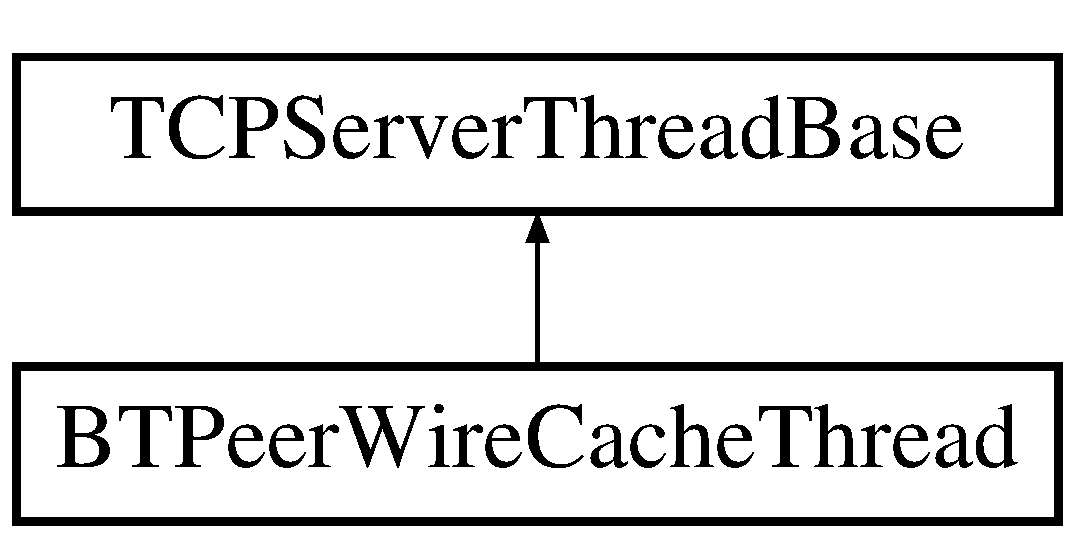
\includegraphics[height=2.000000cm]{classBTPeerWireCacheThread}
\end{center}
\end{figure}
\subsection*{Public Member Functions}
\begin{DoxyCompactItemize}
\item 
\hyperlink{classBTPeerWireCacheThread_a64d59956f320cd1f02a9cd25bb5a9b0e}{B\+T\+Peer\+Wire\+Cache\+Thread} ()
\item 
virtual \hyperlink{classBTPeerWireCacheThread_a53ff411ef0e4195e47a1243f8fbc5890}{$\sim$\+B\+T\+Peer\+Wire\+Cache\+Thread} ()
\item 
virtual void \hyperlink{classBTPeerWireCacheThread_ae2b849a82f1fbc804720d8dbd6a1da03}{init} (T\+C\+P\+Srv\+Host\+App $\ast$hostmodule, T\+C\+P\+Socket $\ast$socket)
\item 
void \hyperlink{classBTPeerWireCacheThread_a25c8569e9f081e494010b52ef49ffc28}{set\+Remote\+Peer\+I\+D} (string)
\item 
string \hyperlink{classBTPeerWireCacheThread_a73e132e3219c223e9a76807b8f690e1c}{get\+Remote\+Peer\+I\+D} ()
\item 
int \hyperlink{classBTPeerWireCacheThread_a1381df92c8aa197f77d2acdb427d9a5c}{get\+State} ()
\item 
void \hyperlink{classBTPeerWireCacheThread_a7011178cc92072e84e221fc9ce0a1b7e}{set\+State} (int)
\item 
bool \hyperlink{classBTPeerWireCacheThread_acaaeb8995d597ff9dacab531989ce7ab}{active\+Connection} ()
\item 
void \hyperlink{classBTPeerWireCacheThread_af3e0310651d1223378f3a80a13e981c9}{set\+Active\+Connection} (bool)
\item 
void \hyperlink{classBTPeerWireCacheThread_ab919706b39311ea8dff25267faa51e73}{send\+Message} (c\+Message $\ast$)
\end{DoxyCompactItemize}
\subsection*{Protected Member Functions}
\begin{DoxyCompactItemize}
\item 
void \hyperlink{classBTPeerWireCacheThread_a99d533084cc41ba0eb431786e611ed67}{close\+Connection} ()
\item 
void \hyperlink{classBTPeerWireCacheThread_a1443d7cf4e65960990d5eafbbdaa38be}{cancel\+Block\+Request} ()
\item 
c\+Message $\ast$ \hyperlink{classBTPeerWireCacheThread_a2877951d5f8147d380840d0964703157}{create\+B\+T\+Peer\+Wire\+Message} (const char $\ast$, int, int, int, int)
\item 
virtual void \hyperlink{classBTPeerWireCacheThread_abd3b5c0f91f4812fbbba05020a219e5d}{established} ()
\item 
virtual void \hyperlink{classBTPeerWireCacheThread_a2e60ec0775d674781d177982c6cadad9}{data\+Arrived} (c\+Message $\ast$, bool)
\item 
virtual void \hyperlink{classBTPeerWireCacheThread_ab65e46311fbacfb79e046d132cc626d6}{timer\+Expired} (c\+Message $\ast$)
\item 
virtual void \hyperlink{classBTPeerWireCacheThread_a010c0f0560e66bcecfe1a2a144f04d2d}{peer\+Closed} ()
\item 
virtual void \hyperlink{classBTPeerWireCacheThread_aa155e51409bf401597d3359f5106edf8}{closed} ()
\item 
virtual void \hyperlink{classBTPeerWireCacheThread_a7c1707a8368a36f544279a7e76b4295d}{failure} (int)
\end{DoxyCompactItemize}
\subsection*{Protected Attributes}
\begin{DoxyCompactItemize}
\item 
\hyperlink{classBTPeerWireBase}{B\+T\+Peer\+Wire\+Base} $\ast$ \hyperlink{classBTPeerWireCacheThread_a3b3958e3db0092891e2316c5867b93c4}{peer\+Wire\+Base}
\item 
string \hyperlink{classBTPeerWireCacheThread_a63ec54a272a54c81f7900e5a8cdf5f8a}{remote\+Cache\+I\+D\+\_\+var}
\item 
int \hyperlink{classBTPeerWireCacheThread_ab0fe60bb80ce09de5bc14153075af0b7}{state\+\_\+var}
\item 
bool \hyperlink{classBTPeerWireCacheThread_ab2d101d565b86e392386a1140feae26a}{active\+Connection\+\_\+var}
\end{DoxyCompactItemize}


\subsection{Constructor \& Destructor Documentation}
\hypertarget{classBTPeerWireCacheThread_a64d59956f320cd1f02a9cd25bb5a9b0e}{}\index{B\+T\+Peer\+Wire\+Cache\+Thread@{B\+T\+Peer\+Wire\+Cache\+Thread}!B\+T\+Peer\+Wire\+Cache\+Thread@{B\+T\+Peer\+Wire\+Cache\+Thread}}
\index{B\+T\+Peer\+Wire\+Cache\+Thread@{B\+T\+Peer\+Wire\+Cache\+Thread}!B\+T\+Peer\+Wire\+Cache\+Thread@{B\+T\+Peer\+Wire\+Cache\+Thread}}
\subsubsection[{B\+T\+Peer\+Wire\+Cache\+Thread()}]{\setlength{\rightskip}{0pt plus 5cm}B\+T\+Peer\+Wire\+Cache\+Thread\+::\+B\+T\+Peer\+Wire\+Cache\+Thread (
\begin{DoxyParamCaption}
{}
\end{DoxyParamCaption}
)}\label{classBTPeerWireCacheThread_a64d59956f320cd1f02a9cd25bb5a9b0e}
\hypertarget{classBTPeerWireCacheThread_a53ff411ef0e4195e47a1243f8fbc5890}{}\index{B\+T\+Peer\+Wire\+Cache\+Thread@{B\+T\+Peer\+Wire\+Cache\+Thread}!````~B\+T\+Peer\+Wire\+Cache\+Thread@{$\sim$\+B\+T\+Peer\+Wire\+Cache\+Thread}}
\index{````~B\+T\+Peer\+Wire\+Cache\+Thread@{$\sim$\+B\+T\+Peer\+Wire\+Cache\+Thread}!B\+T\+Peer\+Wire\+Cache\+Thread@{B\+T\+Peer\+Wire\+Cache\+Thread}}
\subsubsection[{$\sim$\+B\+T\+Peer\+Wire\+Cache\+Thread()}]{\setlength{\rightskip}{0pt plus 5cm}B\+T\+Peer\+Wire\+Cache\+Thread\+::$\sim$\+B\+T\+Peer\+Wire\+Cache\+Thread (
\begin{DoxyParamCaption}
{}
\end{DoxyParamCaption}
)\hspace{0.3cm}{\ttfamily [virtual]}}\label{classBTPeerWireCacheThread_a53ff411ef0e4195e47a1243f8fbc5890}


\subsection{Member Function Documentation}
\hypertarget{classBTPeerWireCacheThread_acaaeb8995d597ff9dacab531989ce7ab}{}\index{B\+T\+Peer\+Wire\+Cache\+Thread@{B\+T\+Peer\+Wire\+Cache\+Thread}!active\+Connection@{active\+Connection}}
\index{active\+Connection@{active\+Connection}!B\+T\+Peer\+Wire\+Cache\+Thread@{B\+T\+Peer\+Wire\+Cache\+Thread}}
\subsubsection[{active\+Connection()}]{\setlength{\rightskip}{0pt plus 5cm}bool B\+T\+Peer\+Wire\+Cache\+Thread\+::active\+Connection (
\begin{DoxyParamCaption}
{}
\end{DoxyParamCaption}
)}\label{classBTPeerWireCacheThread_acaaeb8995d597ff9dacab531989ce7ab}
\hypertarget{classBTPeerWireCacheThread_a1443d7cf4e65960990d5eafbbdaa38be}{}\index{B\+T\+Peer\+Wire\+Cache\+Thread@{B\+T\+Peer\+Wire\+Cache\+Thread}!cancel\+Block\+Request@{cancel\+Block\+Request}}
\index{cancel\+Block\+Request@{cancel\+Block\+Request}!B\+T\+Peer\+Wire\+Cache\+Thread@{B\+T\+Peer\+Wire\+Cache\+Thread}}
\subsubsection[{cancel\+Block\+Request()}]{\setlength{\rightskip}{0pt plus 5cm}void B\+T\+Peer\+Wire\+Cache\+Thread\+::cancel\+Block\+Request (
\begin{DoxyParamCaption}
{}
\end{DoxyParamCaption}
)\hspace{0.3cm}{\ttfamily [protected]}}\label{classBTPeerWireCacheThread_a1443d7cf4e65960990d5eafbbdaa38be}
\hypertarget{classBTPeerWireCacheThread_a99d533084cc41ba0eb431786e611ed67}{}\index{B\+T\+Peer\+Wire\+Cache\+Thread@{B\+T\+Peer\+Wire\+Cache\+Thread}!close\+Connection@{close\+Connection}}
\index{close\+Connection@{close\+Connection}!B\+T\+Peer\+Wire\+Cache\+Thread@{B\+T\+Peer\+Wire\+Cache\+Thread}}
\subsubsection[{close\+Connection()}]{\setlength{\rightskip}{0pt plus 5cm}void B\+T\+Peer\+Wire\+Cache\+Thread\+::close\+Connection (
\begin{DoxyParamCaption}
{}
\end{DoxyParamCaption}
)\hspace{0.3cm}{\ttfamily [protected]}}\label{classBTPeerWireCacheThread_a99d533084cc41ba0eb431786e611ed67}
\hypertarget{classBTPeerWireCacheThread_aa155e51409bf401597d3359f5106edf8}{}\index{B\+T\+Peer\+Wire\+Cache\+Thread@{B\+T\+Peer\+Wire\+Cache\+Thread}!closed@{closed}}
\index{closed@{closed}!B\+T\+Peer\+Wire\+Cache\+Thread@{B\+T\+Peer\+Wire\+Cache\+Thread}}
\subsubsection[{closed()}]{\setlength{\rightskip}{0pt plus 5cm}void B\+T\+Peer\+Wire\+Cache\+Thread\+::closed (
\begin{DoxyParamCaption}
{}
\end{DoxyParamCaption}
)\hspace{0.3cm}{\ttfamily [protected]}, {\ttfamily [virtual]}}\label{classBTPeerWireCacheThread_aa155e51409bf401597d3359f5106edf8}
\hypertarget{classBTPeerWireCacheThread_a2877951d5f8147d380840d0964703157}{}\index{B\+T\+Peer\+Wire\+Cache\+Thread@{B\+T\+Peer\+Wire\+Cache\+Thread}!create\+B\+T\+Peer\+Wire\+Message@{create\+B\+T\+Peer\+Wire\+Message}}
\index{create\+B\+T\+Peer\+Wire\+Message@{create\+B\+T\+Peer\+Wire\+Message}!B\+T\+Peer\+Wire\+Cache\+Thread@{B\+T\+Peer\+Wire\+Cache\+Thread}}
\subsubsection[{create\+B\+T\+Peer\+Wire\+Message(const char $\ast$, int, int, int, int)}]{\setlength{\rightskip}{0pt plus 5cm}c\+Message $\ast$ B\+T\+Peer\+Wire\+Cache\+Thread\+::create\+B\+T\+Peer\+Wire\+Message (
\begin{DoxyParamCaption}
\item[{const char $\ast$}]{name, }
\item[{int}]{kind, }
\item[{int}]{index, }
\item[{int}]{begin, }
\item[{int}]{length}
\end{DoxyParamCaption}
)\hspace{0.3cm}{\ttfamily [protected]}}\label{classBTPeerWireCacheThread_a2877951d5f8147d380840d0964703157}
\hypertarget{classBTPeerWireCacheThread_a2e60ec0775d674781d177982c6cadad9}{}\index{B\+T\+Peer\+Wire\+Cache\+Thread@{B\+T\+Peer\+Wire\+Cache\+Thread}!data\+Arrived@{data\+Arrived}}
\index{data\+Arrived@{data\+Arrived}!B\+T\+Peer\+Wire\+Cache\+Thread@{B\+T\+Peer\+Wire\+Cache\+Thread}}
\subsubsection[{data\+Arrived(c\+Message $\ast$, bool)}]{\setlength{\rightskip}{0pt plus 5cm}void B\+T\+Peer\+Wire\+Cache\+Thread\+::data\+Arrived (
\begin{DoxyParamCaption}
\item[{c\+Message $\ast$}]{mmsg, }
\item[{bool}]{bool1}
\end{DoxyParamCaption}
)\hspace{0.3cm}{\ttfamily [protected]}, {\ttfamily [virtual]}}\label{classBTPeerWireCacheThread_a2e60ec0775d674781d177982c6cadad9}
\hypertarget{classBTPeerWireCacheThread_abd3b5c0f91f4812fbbba05020a219e5d}{}\index{B\+T\+Peer\+Wire\+Cache\+Thread@{B\+T\+Peer\+Wire\+Cache\+Thread}!established@{established}}
\index{established@{established}!B\+T\+Peer\+Wire\+Cache\+Thread@{B\+T\+Peer\+Wire\+Cache\+Thread}}
\subsubsection[{established()}]{\setlength{\rightskip}{0pt plus 5cm}void B\+T\+Peer\+Wire\+Cache\+Thread\+::established (
\begin{DoxyParamCaption}
{}
\end{DoxyParamCaption}
)\hspace{0.3cm}{\ttfamily [protected]}, {\ttfamily [virtual]}}\label{classBTPeerWireCacheThread_abd3b5c0f91f4812fbbba05020a219e5d}
\hypertarget{classBTPeerWireCacheThread_a7c1707a8368a36f544279a7e76b4295d}{}\index{B\+T\+Peer\+Wire\+Cache\+Thread@{B\+T\+Peer\+Wire\+Cache\+Thread}!failure@{failure}}
\index{failure@{failure}!B\+T\+Peer\+Wire\+Cache\+Thread@{B\+T\+Peer\+Wire\+Cache\+Thread}}
\subsubsection[{failure(int)}]{\setlength{\rightskip}{0pt plus 5cm}void B\+T\+Peer\+Wire\+Cache\+Thread\+::failure (
\begin{DoxyParamCaption}
\item[{int}]{code}
\end{DoxyParamCaption}
)\hspace{0.3cm}{\ttfamily [protected]}, {\ttfamily [virtual]}}\label{classBTPeerWireCacheThread_a7c1707a8368a36f544279a7e76b4295d}
\hypertarget{classBTPeerWireCacheThread_a73e132e3219c223e9a76807b8f690e1c}{}\index{B\+T\+Peer\+Wire\+Cache\+Thread@{B\+T\+Peer\+Wire\+Cache\+Thread}!get\+Remote\+Peer\+I\+D@{get\+Remote\+Peer\+I\+D}}
\index{get\+Remote\+Peer\+I\+D@{get\+Remote\+Peer\+I\+D}!B\+T\+Peer\+Wire\+Cache\+Thread@{B\+T\+Peer\+Wire\+Cache\+Thread}}
\subsubsection[{get\+Remote\+Peer\+I\+D()}]{\setlength{\rightskip}{0pt plus 5cm}string B\+T\+Peer\+Wire\+Cache\+Thread\+::get\+Remote\+Peer\+I\+D (
\begin{DoxyParamCaption}
{}
\end{DoxyParamCaption}
)}\label{classBTPeerWireCacheThread_a73e132e3219c223e9a76807b8f690e1c}
\hypertarget{classBTPeerWireCacheThread_a1381df92c8aa197f77d2acdb427d9a5c}{}\index{B\+T\+Peer\+Wire\+Cache\+Thread@{B\+T\+Peer\+Wire\+Cache\+Thread}!get\+State@{get\+State}}
\index{get\+State@{get\+State}!B\+T\+Peer\+Wire\+Cache\+Thread@{B\+T\+Peer\+Wire\+Cache\+Thread}}
\subsubsection[{get\+State()}]{\setlength{\rightskip}{0pt plus 5cm}int B\+T\+Peer\+Wire\+Cache\+Thread\+::get\+State (
\begin{DoxyParamCaption}
{}
\end{DoxyParamCaption}
)}\label{classBTPeerWireCacheThread_a1381df92c8aa197f77d2acdb427d9a5c}
\hypertarget{classBTPeerWireCacheThread_ae2b849a82f1fbc804720d8dbd6a1da03}{}\index{B\+T\+Peer\+Wire\+Cache\+Thread@{B\+T\+Peer\+Wire\+Cache\+Thread}!init@{init}}
\index{init@{init}!B\+T\+Peer\+Wire\+Cache\+Thread@{B\+T\+Peer\+Wire\+Cache\+Thread}}
\subsubsection[{init(\+T\+C\+P\+Srv\+Host\+App $\ast$hostmodule, T\+C\+P\+Socket $\ast$socket)}]{\setlength{\rightskip}{0pt plus 5cm}void B\+T\+Peer\+Wire\+Cache\+Thread\+::init (
\begin{DoxyParamCaption}
\item[{T\+C\+P\+Srv\+Host\+App $\ast$}]{hostmodule, }
\item[{T\+C\+P\+Socket $\ast$}]{socket}
\end{DoxyParamCaption}
)\hspace{0.3cm}{\ttfamily [virtual]}}\label{classBTPeerWireCacheThread_ae2b849a82f1fbc804720d8dbd6a1da03}
\hypertarget{classBTPeerWireCacheThread_a010c0f0560e66bcecfe1a2a144f04d2d}{}\index{B\+T\+Peer\+Wire\+Cache\+Thread@{B\+T\+Peer\+Wire\+Cache\+Thread}!peer\+Closed@{peer\+Closed}}
\index{peer\+Closed@{peer\+Closed}!B\+T\+Peer\+Wire\+Cache\+Thread@{B\+T\+Peer\+Wire\+Cache\+Thread}}
\subsubsection[{peer\+Closed()}]{\setlength{\rightskip}{0pt plus 5cm}void B\+T\+Peer\+Wire\+Cache\+Thread\+::peer\+Closed (
\begin{DoxyParamCaption}
{}
\end{DoxyParamCaption}
)\hspace{0.3cm}{\ttfamily [protected]}, {\ttfamily [virtual]}}\label{classBTPeerWireCacheThread_a010c0f0560e66bcecfe1a2a144f04d2d}
\hypertarget{classBTPeerWireCacheThread_ab919706b39311ea8dff25267faa51e73}{}\index{B\+T\+Peer\+Wire\+Cache\+Thread@{B\+T\+Peer\+Wire\+Cache\+Thread}!send\+Message@{send\+Message}}
\index{send\+Message@{send\+Message}!B\+T\+Peer\+Wire\+Cache\+Thread@{B\+T\+Peer\+Wire\+Cache\+Thread}}
\subsubsection[{send\+Message(c\+Message $\ast$)}]{\setlength{\rightskip}{0pt plus 5cm}void B\+T\+Peer\+Wire\+Cache\+Thread\+::send\+Message (
\begin{DoxyParamCaption}
\item[{c\+Message $\ast$}]{mmsg}
\end{DoxyParamCaption}
)}\label{classBTPeerWireCacheThread_ab919706b39311ea8dff25267faa51e73}
\hypertarget{classBTPeerWireCacheThread_af3e0310651d1223378f3a80a13e981c9}{}\index{B\+T\+Peer\+Wire\+Cache\+Thread@{B\+T\+Peer\+Wire\+Cache\+Thread}!set\+Active\+Connection@{set\+Active\+Connection}}
\index{set\+Active\+Connection@{set\+Active\+Connection}!B\+T\+Peer\+Wire\+Cache\+Thread@{B\+T\+Peer\+Wire\+Cache\+Thread}}
\subsubsection[{set\+Active\+Connection(bool)}]{\setlength{\rightskip}{0pt plus 5cm}void B\+T\+Peer\+Wire\+Cache\+Thread\+::set\+Active\+Connection (
\begin{DoxyParamCaption}
\item[{bool}]{con}
\end{DoxyParamCaption}
)}\label{classBTPeerWireCacheThread_af3e0310651d1223378f3a80a13e981c9}
\hypertarget{classBTPeerWireCacheThread_a25c8569e9f081e494010b52ef49ffc28}{}\index{B\+T\+Peer\+Wire\+Cache\+Thread@{B\+T\+Peer\+Wire\+Cache\+Thread}!set\+Remote\+Peer\+I\+D@{set\+Remote\+Peer\+I\+D}}
\index{set\+Remote\+Peer\+I\+D@{set\+Remote\+Peer\+I\+D}!B\+T\+Peer\+Wire\+Cache\+Thread@{B\+T\+Peer\+Wire\+Cache\+Thread}}
\subsubsection[{set\+Remote\+Peer\+I\+D(string)}]{\setlength{\rightskip}{0pt plus 5cm}void B\+T\+Peer\+Wire\+Cache\+Thread\+::set\+Remote\+Peer\+I\+D (
\begin{DoxyParamCaption}
\item[{string}]{cache\+I\+D}
\end{DoxyParamCaption}
)}\label{classBTPeerWireCacheThread_a25c8569e9f081e494010b52ef49ffc28}
\hypertarget{classBTPeerWireCacheThread_a7011178cc92072e84e221fc9ce0a1b7e}{}\index{B\+T\+Peer\+Wire\+Cache\+Thread@{B\+T\+Peer\+Wire\+Cache\+Thread}!set\+State@{set\+State}}
\index{set\+State@{set\+State}!B\+T\+Peer\+Wire\+Cache\+Thread@{B\+T\+Peer\+Wire\+Cache\+Thread}}
\subsubsection[{set\+State(int)}]{\setlength{\rightskip}{0pt plus 5cm}void B\+T\+Peer\+Wire\+Cache\+Thread\+::set\+State (
\begin{DoxyParamCaption}
\item[{int}]{state}
\end{DoxyParamCaption}
)}\label{classBTPeerWireCacheThread_a7011178cc92072e84e221fc9ce0a1b7e}
\hypertarget{classBTPeerWireCacheThread_ab65e46311fbacfb79e046d132cc626d6}{}\index{B\+T\+Peer\+Wire\+Cache\+Thread@{B\+T\+Peer\+Wire\+Cache\+Thread}!timer\+Expired@{timer\+Expired}}
\index{timer\+Expired@{timer\+Expired}!B\+T\+Peer\+Wire\+Cache\+Thread@{B\+T\+Peer\+Wire\+Cache\+Thread}}
\subsubsection[{timer\+Expired(c\+Message $\ast$)}]{\setlength{\rightskip}{0pt plus 5cm}void B\+T\+Peer\+Wire\+Cache\+Thread\+::timer\+Expired (
\begin{DoxyParamCaption}
\item[{c\+Message $\ast$}]{timer}
\end{DoxyParamCaption}
)\hspace{0.3cm}{\ttfamily [protected]}, {\ttfamily [virtual]}}\label{classBTPeerWireCacheThread_ab65e46311fbacfb79e046d132cc626d6}


\subsection{Member Data Documentation}
\hypertarget{classBTPeerWireCacheThread_ab2d101d565b86e392386a1140feae26a}{}\index{B\+T\+Peer\+Wire\+Cache\+Thread@{B\+T\+Peer\+Wire\+Cache\+Thread}!active\+Connection\+\_\+var@{active\+Connection\+\_\+var}}
\index{active\+Connection\+\_\+var@{active\+Connection\+\_\+var}!B\+T\+Peer\+Wire\+Cache\+Thread@{B\+T\+Peer\+Wire\+Cache\+Thread}}
\subsubsection[{active\+Connection\+\_\+var}]{\setlength{\rightskip}{0pt plus 5cm}bool B\+T\+Peer\+Wire\+Cache\+Thread\+::active\+Connection\+\_\+var\hspace{0.3cm}{\ttfamily [protected]}}\label{classBTPeerWireCacheThread_ab2d101d565b86e392386a1140feae26a}
\hypertarget{classBTPeerWireCacheThread_a3b3958e3db0092891e2316c5867b93c4}{}\index{B\+T\+Peer\+Wire\+Cache\+Thread@{B\+T\+Peer\+Wire\+Cache\+Thread}!peer\+Wire\+Base@{peer\+Wire\+Base}}
\index{peer\+Wire\+Base@{peer\+Wire\+Base}!B\+T\+Peer\+Wire\+Cache\+Thread@{B\+T\+Peer\+Wire\+Cache\+Thread}}
\subsubsection[{peer\+Wire\+Base}]{\setlength{\rightskip}{0pt plus 5cm}{\bf B\+T\+Peer\+Wire\+Base}$\ast$ B\+T\+Peer\+Wire\+Cache\+Thread\+::peer\+Wire\+Base\hspace{0.3cm}{\ttfamily [protected]}}\label{classBTPeerWireCacheThread_a3b3958e3db0092891e2316c5867b93c4}
\hypertarget{classBTPeerWireCacheThread_a63ec54a272a54c81f7900e5a8cdf5f8a}{}\index{B\+T\+Peer\+Wire\+Cache\+Thread@{B\+T\+Peer\+Wire\+Cache\+Thread}!remote\+Cache\+I\+D\+\_\+var@{remote\+Cache\+I\+D\+\_\+var}}
\index{remote\+Cache\+I\+D\+\_\+var@{remote\+Cache\+I\+D\+\_\+var}!B\+T\+Peer\+Wire\+Cache\+Thread@{B\+T\+Peer\+Wire\+Cache\+Thread}}
\subsubsection[{remote\+Cache\+I\+D\+\_\+var}]{\setlength{\rightskip}{0pt plus 5cm}string B\+T\+Peer\+Wire\+Cache\+Thread\+::remote\+Cache\+I\+D\+\_\+var\hspace{0.3cm}{\ttfamily [protected]}}\label{classBTPeerWireCacheThread_a63ec54a272a54c81f7900e5a8cdf5f8a}
\hypertarget{classBTPeerWireCacheThread_ab0fe60bb80ce09de5bc14153075af0b7}{}\index{B\+T\+Peer\+Wire\+Cache\+Thread@{B\+T\+Peer\+Wire\+Cache\+Thread}!state\+\_\+var@{state\+\_\+var}}
\index{state\+\_\+var@{state\+\_\+var}!B\+T\+Peer\+Wire\+Cache\+Thread@{B\+T\+Peer\+Wire\+Cache\+Thread}}
\subsubsection[{state\+\_\+var}]{\setlength{\rightskip}{0pt plus 5cm}int B\+T\+Peer\+Wire\+Cache\+Thread\+::state\+\_\+var\hspace{0.3cm}{\ttfamily [protected]}}\label{classBTPeerWireCacheThread_ab0fe60bb80ce09de5bc14153075af0b7}


The documentation for this class was generated from the following files\+:\begin{DoxyCompactItemize}
\item 
\hyperlink{BTPeerWireCacheThread_8h}{B\+T\+Peer\+Wire\+Cache\+Thread.\+h}\item 
\hyperlink{BTPeerWireCacheThread_8cc}{B\+T\+Peer\+Wire\+Cache\+Thread.\+cc}\end{DoxyCompactItemize}

\hypertarget{classBTPeerWireClientHandlerBase}{}\section{B\+T\+Peer\+Wire\+Client\+Handler\+Base Class Reference}
\label{classBTPeerWireClientHandlerBase}\index{B\+T\+Peer\+Wire\+Client\+Handler\+Base@{B\+T\+Peer\+Wire\+Client\+Handler\+Base}}


{\ttfamily \#include $<$B\+T\+Peer\+Wire\+Client\+Handler\+Base.\+h$>$}

Inheritance diagram for B\+T\+Peer\+Wire\+Client\+Handler\+Base\+:\begin{figure}[H]
\begin{center}
\leavevmode
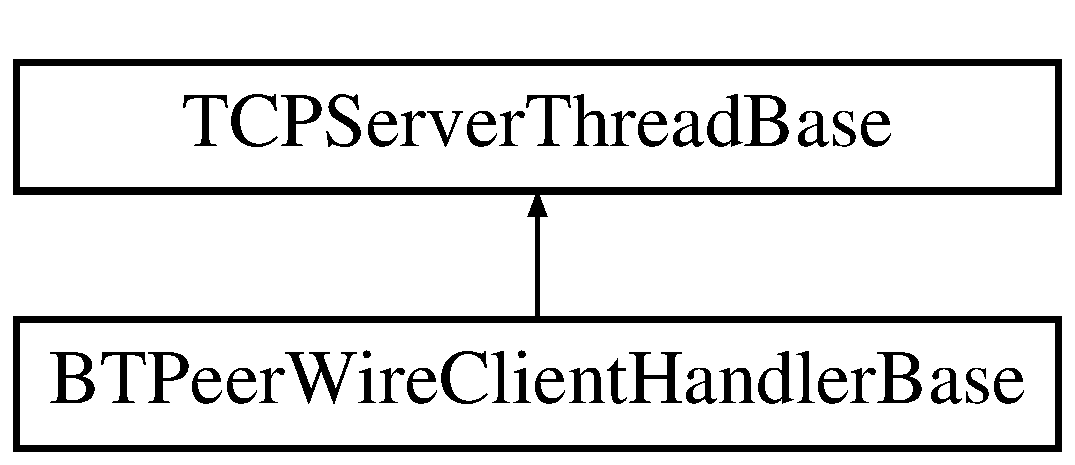
\includegraphics[height=2.000000cm]{classBTPeerWireClientHandlerBase}
\end{center}
\end{figure}
\subsection*{Public Member Functions}
\begin{DoxyCompactItemize}
\item 
\hyperlink{classBTPeerWireClientHandlerBase_ac7325e2bd56ed10022900f02163b0c1f}{B\+T\+Peer\+Wire\+Client\+Handler\+Base} ()
\item 
virtual \hyperlink{classBTPeerWireClientHandlerBase_a5f7019d47fdcf107d6ec2bfaeeb503fc}{$\sim$\+B\+T\+Peer\+Wire\+Client\+Handler\+Base} ()
\item 
c\+Message $\ast$ \hyperlink{classBTPeerWireClientHandlerBase_a9d8b08a5439211d0bb8329a162873507}{create\+B\+T\+Peer\+Wire\+Message} (const char $\ast$, int)
\item 
c\+Message $\ast$ \hyperlink{classBTPeerWireClientHandlerBase_afd0a266c3f5974f73bece07d10958433}{create\+B\+T\+Peer\+Wire\+Message} (const char $\ast$, int, int, int, int)
\item 
virtual void \hyperlink{classBTPeerWireClientHandlerBase_a45da9fc8b5c7775ccd8c655f01daa94d}{init} (T\+C\+P\+Srv\+Host\+App $\ast$hostmodule, T\+C\+P\+Socket $\ast$socket)
\item 
void \hyperlink{classBTPeerWireClientHandlerBase_a6be659855aedc7329581b0126a3a2f91}{send\+Block\+Requests} (int, int)
\item 
void \hyperlink{classBTPeerWireClientHandlerBase_a6cd1b6f7c992e161427270ea22d7e0bb}{send\+End\+Game\+Block\+Requests} (int, int)
\item 
void \hyperlink{classBTPeerWireClientHandlerBase_a23f4981ac7567bd8de2e3abfe09e0e59}{set\+Remote\+Peer\+I\+D} (string)
\item 
string \hyperlink{classBTPeerWireClientHandlerBase_ae628b93afb6883201da0457b43f7d02a}{get\+Remote\+Peer\+I\+D} ()
\item 
\hyperlink{classBitField}{Bit\+Field} $\ast$ \hyperlink{classBTPeerWireClientHandlerBase_a4345688ea84e947d57f9da6e32633628}{get\+Remote\+Bitfield} ()
\item 
httpt\+Request\+Message $\ast$ \hyperlink{classBTPeerWireClientHandlerBase_a8adacdf80a2b2e27e43e4646656a81e3}{build\+Http\+Request} (\hyperlink{classBTRequestCancelMsg}{B\+T\+Request\+Cancel\+Msg} $\ast$)
\item 
bool \hyperlink{classBTPeerWireClientHandlerBase_a93eef1a2a5e75b5e38e4d26c5b3fc4c2}{am\+Choking} ()
\item 
void \hyperlink{classBTPeerWireClientHandlerBase_a1e570420131edef266b7321f61aed75a}{set\+Am\+Choking} (bool)
\item 
bool \hyperlink{classBTPeerWireClientHandlerBase_aec48d715bfaa4a5eed2ee91f42af1491}{am\+Interested} ()
\item 
void \hyperlink{classBTPeerWireClientHandlerBase_a24864559c78e2de1c25bdb381e083a01}{set\+Am\+Interested} (bool)
\item 
bool \hyperlink{classBTPeerWireClientHandlerBase_a8349a5110429c914d3012f7ab6cf858d}{peer\+Choking} ()
\item 
void \hyperlink{classBTPeerWireClientHandlerBase_a068cc1c357432956497371e0444974eb}{set\+Peer\+Choking} (bool)
\item 
bool \hyperlink{classBTPeerWireClientHandlerBase_ae01019632db70656410a2fd7a5b13707}{peer\+Interested} ()
\item 
void \hyperlink{classBTPeerWireClientHandlerBase_ab7d665b269ef7f0ae6d1d2beaa038ecd}{set\+Peer\+Interested} (bool)
\item 
float \hyperlink{classBTPeerWireClientHandlerBase_a656939f502f38131e6af0d730d752424}{get\+Download\+Rate} ()
\item 
void \hyperlink{classBTPeerWireClientHandlerBase_a1a6e44e8e008679a3ea57dd8426d78e1}{set\+Download\+Rate} (float)
\item 
float \hyperlink{classBTPeerWireClientHandlerBase_aed2663507bd8ed48d7633a939bcacade}{get\+Upload\+Rate} ()
\item 
void \hyperlink{classBTPeerWireClientHandlerBase_a8724c1ba138d3cdea58c6432dad21426}{set\+Upload\+Rate} (float)
\item 
bool \hyperlink{classBTPeerWireClientHandlerBase_a53c834eccb77e823da90874c2fb77307}{seeder} ()
\item 
void \hyperlink{classBTPeerWireClientHandlerBase_a856d49c4e1caf16b0fd2e08b708e7cb5}{set\+Seeder} (bool)
\item 
simtime\+\_\+t \hyperlink{classBTPeerWireClientHandlerBase_ad373932a15efbef51164347aa36fcd7d}{connect\+Time\+Shift} ()
\item 
void \hyperlink{classBTPeerWireClientHandlerBase_af41240e2d031bf252137c4ada0ed29fb}{set\+Connect\+Time\+Shift} (simtime\+\_\+t)
\item 
bool \hyperlink{classBTPeerWireClientHandlerBase_ad6346252c972215582a0cf54dd5ae4c1}{is\+Optimistically\+Unchoked} ()
\item 
void \hyperlink{classBTPeerWireClientHandlerBase_ae6a50a41c2dd39d3b22c5e9d4c60aeef}{set\+Optimistically\+Unchoked} (bool)
\item 
void \hyperlink{classBTPeerWireClientHandlerBase_ac21015df428f260f56965b779bb493a1}{clear\+Pending\+Requests} ()
\item 
void \hyperlink{classBTPeerWireClientHandlerBase_ae8fde71b4845f5b438ad25941ab1ed32}{clear\+Pending\+Incoming\+Requests} ()
\item 
\hyperlink{classRequestState}{Request\+State} \hyperlink{classBTPeerWireClientHandlerBase_a4a2bdba08d9795abd9cacd490f7f7fa2}{get\+Requests} ()
\item 
int \hyperlink{classBTPeerWireClientHandlerBase_a9d436de27e234b7ea6efe98b89d5dda5}{get\+Num\+Pending\+Requests} ()
\item 
void \hyperlink{classBTPeerWireClientHandlerBase_aafc909e05d47fd83120e446a599a340a}{increase\+Request\+Queue\+Size} (int)
\item 
int \hyperlink{classBTPeerWireClientHandlerBase_ad472fb16748702d6e06bfeb182672c97}{get\+State} ()
\item 
void \hyperlink{classBTPeerWireClientHandlerBase_ac6b9ceaf497a1163468150b8608b3010}{set\+State} (int)
\item 
simtime\+\_\+t \hyperlink{classBTPeerWireClientHandlerBase_a98b88b4b0c373fb76bb8c85ff37ff846}{last\+Choke\+Unchoke} ()
\item 
void \hyperlink{classBTPeerWireClientHandlerBase_aee003ca2d11ee81b58d4855b9be19941}{set\+Last\+Choke\+Unchoke} (simtime\+\_\+t)
\item 
bool \hyperlink{classBTPeerWireClientHandlerBase_a5bd0e7aff2b810be26acf654354ad4f3}{allowed\+To\+Request} ()
\item 
void \hyperlink{classBTPeerWireClientHandlerBase_a76120fc420e710b81ce55313d8c5e6a3}{set\+Allowed\+To\+Request} (bool)
\item 
bool \hyperlink{classBTPeerWireClientHandlerBase_a03541b3c0f171b1c7765d171b1036ee2}{in\+End\+Game} ()
\item 
void \hyperlink{classBTPeerWireClientHandlerBase_a73e9ccd9f9875ef47afe345bf423939c}{set\+In\+End\+Game} (bool)
\item 
bool \hyperlink{classBTPeerWireClientHandlerBase_aed3f62796a8c80716179037931ca5705}{active\+Connection} ()
\item 
void \hyperlink{classBTPeerWireClientHandlerBase_aa8a49edb676980255f080c0692c33ce0}{set\+Active\+Connection} (bool)
\item 
const char $\ast$ \hyperlink{classBTPeerWireClientHandlerBase_a1d74bfc2beb178cec5d9b48c776c9ec5}{socket\+State} ()
\item 
void \hyperlink{classBTPeerWireClientHandlerBase_ad5c1656f8249bb62929224375dba07ff}{update\+Dowload\+Rate} (\hyperlink{classBTPieceMsg}{B\+T\+Piece\+Msg} $\ast$, int)
\item 
void \hyperlink{classBTPeerWireClientHandlerBase_a27b8eeb61b70127ac8d7652ba1f3fc3a}{update\+Upload\+Rate} (\hyperlink{classRequestEntry}{Request\+Entry})
\item 
void \hyperlink{classBTPeerWireClientHandlerBase_aee6a16181b8ea89f33862f78471374e4}{update\+Correspondent\+Thread\+Upload\+Rate} (\hyperlink{classRequestEntry}{Request\+Entry})
\item 
bool \hyperlink{classBTPeerWireClientHandlerBase_a159dcf796c87781115918534fc7b0fb7}{is\+Cache\+Thread} ()
\item 
void \hyperlink{classBTPeerWireClientHandlerBase_a90af0cb4b355088def3f758a907fbf17}{set\+Is\+Cache\+Thread} (bool)
\end{DoxyCompactItemize}
\subsection*{Public Attributes}
\begin{DoxyCompactItemize}
\item 
\hyperlink{classRequestState}{Request\+State} \hyperlink{classBTPeerWireClientHandlerBase_aa01cf33d132d58a3fd326978b0233ee5}{incoming\+Requests}
\end{DoxyCompactItemize}
\subsection*{Protected Member Functions}
\begin{DoxyCompactItemize}
\item 
void \hyperlink{classBTPeerWireClientHandlerBase_a64bb0a6c6a300c49219c3b76e48cfeb3}{close\+Connection} ()
\item 
void \hyperlink{classBTPeerWireClientHandlerBase_a1554aa617935544f997fcafbd27f7042}{remove\+Current\+Thread} ()
\item 
void \hyperlink{classBTPeerWireClientHandlerBase_ad8d40ee69f8d37e525ffd7e046192a8a}{renew\+Alive\+Timer} (c\+Message $\ast$)
\item 
void \hyperlink{classBTPeerWireClientHandlerBase_a940cd9fe9eaeefac82a1ba40f260f87f}{renew\+Anti\+Snub\+Timer} ()
\item 
void \hyperlink{classBTPeerWireClientHandlerBase_a82e3be625984c86701e0ac15f129cb20}{cancel\+Block\+Request} (\hyperlink{classBTRequestCancelMsg}{B\+T\+Request\+Cancel\+Msg} $\ast$)
\item 
void \hyperlink{classBTPeerWireClientHandlerBase_afd4e172043bf70460281d18c13b04a94}{cancel\+Incoming\+Block\+Requests} ()
\item 
void \hyperlink{classBTPeerWireClientHandlerBase_afee4cdc1b8788aeb4fc8004475c21344}{send\+Message} (c\+Message $\ast$)
\item 
void \hyperlink{classBTPeerWireClientHandlerBase_a8edba6c080d26e7b0b6b24000d145883}{cancel\+And\+Delete} (c\+Message $\ast$)
\item 
void \hyperlink{classBTPeerWireClientHandlerBase_ac7cd85f3e43b56f0c297421f11fc6457}{print\+State} ()
\item 
void \hyperlink{classBTPeerWireClientHandlerBase_ad30ffd6cdf219b2b85da3e76e914887d}{handle\+Remote\+Peer\+Message} (c\+Message $\ast$)
\item 
void \hyperlink{classBTPeerWireClientHandlerBase_a4aa8a43a2cea4f7fadf01f0fc1765129}{handle\+Cache\+Message} (c\+Message $\ast$)
\item 
virtual void \hyperlink{classBTPeerWireClientHandlerBase_a78616d6f856688d45cd1e3ea737ac904}{established} ()
\item 
virtual void \hyperlink{classBTPeerWireClientHandlerBase_a0a900fcb7639dab49a18b2a8f35fa0ef}{data\+Arrived} (c\+Message $\ast$, bool)
\item 
virtual void \hyperlink{classBTPeerWireClientHandlerBase_ad78ba790b8cd206d2ada2399f522cea3}{timer\+Expired} (c\+Message $\ast$)
\item 
virtual void \hyperlink{classBTPeerWireClientHandlerBase_a6895a4cacd6dd906c3c3e82cc085ecee}{peer\+Closed} ()
\item 
virtual void \hyperlink{classBTPeerWireClientHandlerBase_a6d9f301342ed5e5d769f4acdc190ff67}{closed} ()
\item 
virtual void \hyperlink{classBTPeerWireClientHandlerBase_a750903f6a338b89671f4aed9b7b8b006}{failure} (int)
\item 
virtual void \hyperlink{classBTPeerWireClientHandlerBase_ae1f3ba905dda5fd9fe9737a7a9196388}{initiate\+Peer\+Wire\+Protocol} (c\+Message $\ast$)
\end{DoxyCompactItemize}
\subsection*{Protected Attributes}
\begin{DoxyCompactItemize}
\item 
c\+Message $\ast$ \hyperlink{classBTPeerWireClientHandlerBase_acc55d5d39f7e06fddf77549a2ff67425}{evt\+Keep\+Alive}
\item 
c\+Message $\ast$ \hyperlink{classBTPeerWireClientHandlerBase_af55d524d592c461ad71a8dc78a6d2e3f}{evt\+Is\+Alive}
\item 
c\+Message $\ast$ \hyperlink{classBTPeerWireClientHandlerBase_a3aa244b8caf784fe747e8b03c61fdac5}{evt\+Del\+Thread}
\item 
c\+Message $\ast$ \hyperlink{classBTPeerWireClientHandlerBase_a854d68cbbdfe22cf59c70ef1a9cfa617}{evt\+Anti\+Snub}
\item 
c\+Message $\ast$ \hyperlink{classBTPeerWireClientHandlerBase_a72c99108037fa5ea8de8b5a740e3d2b2}{evt\+Handshake}
\item 
c\+Message $\ast$ \hyperlink{classBTPeerWireClientHandlerBase_a12f19b014b30e6c89834d85c8bca6817}{evt\+Measure\+Download\+Rate}
\item 
c\+Message $\ast$ \hyperlink{classBTPeerWireClientHandlerBase_adf45936c09a11f77717abd07f411b1e7}{evt\+Measure\+Upload\+Rate}
\item 
\hyperlink{classBTInternalMsg}{B\+T\+Internal\+Msg} $\ast$ \hyperlink{classBTPeerWireClientHandlerBase_aee618de4f918135adb2da435da4f1424}{del\+Thread\+Msg}
\item 
int \hyperlink{classBTPeerWireClientHandlerBase_a053d029148653ba1451f3f2d6513e303}{Keep\+\_\+\+Alive\+\_\+\+Duration}
\item 
\hyperlink{classBTPeerWireBase}{B\+T\+Peer\+Wire\+Base} $\ast$ \hyperlink{classBTPeerWireClientHandlerBase_a159b67e530160916c78fa72be86f97b6}{peer\+Wire\+Base}
\item 
\hyperlink{classBTTrackerClientBase}{B\+T\+Tracker\+Client\+Base} $\ast$ \hyperlink{classBTPeerWireClientHandlerBase_a9c42f83915497b67123ae9232b2ddae5}{tracker\+Client}
\item 
string \hyperlink{classBTPeerWireClientHandlerBase_aafa0a0277ea273ceb2c625135bf57857}{remote\+Peer\+I\+D}
\item 
\hyperlink{classBitField}{Bit\+Field} $\ast$ \hyperlink{classBTPeerWireClientHandlerBase_ac1884399611a6d8814c30ed73d71371e}{remote\+Bitfield}
\item 
bool \hyperlink{classBTPeerWireClientHandlerBase_ab0f5e70d2b13f138ef9f87a1c272d439}{keep\+Alive\+Expired}
\item 
bool \hyperlink{classBTPeerWireClientHandlerBase_a232a0dcff5ea5068ee37ce6feb60d75f}{am\+Choking\+\_\+var}
\item 
bool \hyperlink{classBTPeerWireClientHandlerBase_afd833d1fdbe70b3e22f0d80ebb040942}{am\+Interested\+\_\+var}
\item 
bool \hyperlink{classBTPeerWireClientHandlerBase_af226ba6a190864e05409c566734f31e9}{peer\+Choking\+\_\+var}
\item 
bool \hyperlink{classBTPeerWireClientHandlerBase_ad63929aec8cc95a4db80efff9919516f}{peer\+Interested\+\_\+var}
\item 
bool \hyperlink{classBTPeerWireClientHandlerBase_a6761283c2d4801c427ed94d00fa7ba39}{H\+A\+V\+E\+\_\+\+S\+E\+N\+T\+\_\+\+K\+E\+E\+P\+\_\+\+A\+L\+I\+V\+E}
\item 
bool \hyperlink{classBTPeerWireClientHandlerBase_a0119aa65591b48eab6db03f373c22312}{is\+Cache\+Thread\+\_\+var}
\item 
int \hyperlink{classBTPeerWireClientHandlerBase_a97d1f49189fd7f912b4148b128518f84}{state\+\_\+var}
\item 
bool \hyperlink{classBTPeerWireClientHandlerBase_af4aaf18b3ecce48ba5851f68f2c5c793}{active\+Connection\+\_\+var}
\item 
int \hyperlink{classBTPeerWireClientHandlerBase_aa30272b681919ef32c7c970cb48c7f09}{piece\+Size}
\item 
int \hyperlink{classBTPeerWireClientHandlerBase_a217d740e84250854b887a1d532de3194}{block\+Size}
\item 
simtime\+\_\+t \hyperlink{classBTPeerWireClientHandlerBase_a97d430e045be6c2a9447a154e94a53d0}{connect\+Time\+Shift\+\_\+var}
\item 
simtime\+\_\+t \hyperlink{classBTPeerWireClientHandlerBase_af16f73e12330b3003bf7ebeaab4d5744}{last\+Download\+Time\+\_\+var}
\item 
float \hyperlink{classBTPeerWireClientHandlerBase_a067ff0b7c09c6c772e1d1e7e2acfb1cb}{download\+Rate}
\item 
vector$<$ float $>$ \hyperlink{classBTPeerWireClientHandlerBase_ab64d3371ce1037d35a6e209ad2120523}{download\+Rate\+Samples}
\item 
simtime\+\_\+t \hyperlink{classBTPeerWireClientHandlerBase_abdbac2c435e66c0e23ca4724998cab5e}{last\+Upload\+Time\+\_\+var}
\item 
float \hyperlink{classBTPeerWireClientHandlerBase_afdfbe8c92b63172725568445ddf09ddf}{upload\+Rate}
\item 
vector$<$ float $>$ \hyperlink{classBTPeerWireClientHandlerBase_a14e7dcfe2478465cc7e4d8f715bd5bc2}{upload\+Rate\+Samples}
\item 
bool \hyperlink{classBTPeerWireClientHandlerBase_a4dfd1a6d41107dec5a2f705bc9040ca3}{in\+End\+Game\+\_\+var}
\item 
bool \hyperlink{classBTPeerWireClientHandlerBase_a6bdae2eb034d492ec5ecded7c196ae59}{seeder\+\_\+var}
\item 
bool \hyperlink{classBTPeerWireClientHandlerBase_a51549ed5b841a0cc04ab9d6c31720592}{optimistically\+Unchoked}
\item 
simtime\+\_\+t \hyperlink{classBTPeerWireClientHandlerBase_ac2d85a86b9690c3f5b6ece4437db1747}{last\+Choke\+Unchoke\+\_\+var}
\item 
bool \hyperlink{classBTPeerWireClientHandlerBase_aa454fe745c1328319b01ccf875bef36a}{allowed\+To\+Request\+\_\+var}
\item 
\hyperlink{classRequestState}{Request\+State} \hyperlink{classBTPeerWireClientHandlerBase_a642a6355fb6d1940b96339e583b00578}{requests}
\item 
\hyperlink{classRequestState}{Request\+State} \hyperlink{classBTPeerWireClientHandlerBase_ac277e0f148cbe859d9895d061e397ef4}{choked\+Requests}
\item 
\hyperlink{classRequestState}{Request\+State} \hyperlink{classBTPeerWireClientHandlerBase_a18d077fec81fc4863b065045e953ab8c}{choked\+Incoming\+Requests}
\end{DoxyCompactItemize}


\subsection{Detailed Description}
Handles communication with a remote peer. 

\subsection{Constructor \& Destructor Documentation}
\hypertarget{classBTPeerWireClientHandlerBase_ac7325e2bd56ed10022900f02163b0c1f}{}\index{B\+T\+Peer\+Wire\+Client\+Handler\+Base@{B\+T\+Peer\+Wire\+Client\+Handler\+Base}!B\+T\+Peer\+Wire\+Client\+Handler\+Base@{B\+T\+Peer\+Wire\+Client\+Handler\+Base}}
\index{B\+T\+Peer\+Wire\+Client\+Handler\+Base@{B\+T\+Peer\+Wire\+Client\+Handler\+Base}!B\+T\+Peer\+Wire\+Client\+Handler\+Base@{B\+T\+Peer\+Wire\+Client\+Handler\+Base}}
\subsubsection[{B\+T\+Peer\+Wire\+Client\+Handler\+Base()}]{\setlength{\rightskip}{0pt plus 5cm}B\+T\+Peer\+Wire\+Client\+Handler\+Base\+::\+B\+T\+Peer\+Wire\+Client\+Handler\+Base (
\begin{DoxyParamCaption}
{}
\end{DoxyParamCaption}
)}\label{classBTPeerWireClientHandlerBase_ac7325e2bd56ed10022900f02163b0c1f}
\hypertarget{classBTPeerWireClientHandlerBase_a5f7019d47fdcf107d6ec2bfaeeb503fc}{}\index{B\+T\+Peer\+Wire\+Client\+Handler\+Base@{B\+T\+Peer\+Wire\+Client\+Handler\+Base}!````~B\+T\+Peer\+Wire\+Client\+Handler\+Base@{$\sim$\+B\+T\+Peer\+Wire\+Client\+Handler\+Base}}
\index{````~B\+T\+Peer\+Wire\+Client\+Handler\+Base@{$\sim$\+B\+T\+Peer\+Wire\+Client\+Handler\+Base}!B\+T\+Peer\+Wire\+Client\+Handler\+Base@{B\+T\+Peer\+Wire\+Client\+Handler\+Base}}
\subsubsection[{$\sim$\+B\+T\+Peer\+Wire\+Client\+Handler\+Base()}]{\setlength{\rightskip}{0pt plus 5cm}B\+T\+Peer\+Wire\+Client\+Handler\+Base\+::$\sim$\+B\+T\+Peer\+Wire\+Client\+Handler\+Base (
\begin{DoxyParamCaption}
{}
\end{DoxyParamCaption}
)\hspace{0.3cm}{\ttfamily [virtual]}}\label{classBTPeerWireClientHandlerBase_a5f7019d47fdcf107d6ec2bfaeeb503fc}


\subsection{Member Function Documentation}
\hypertarget{classBTPeerWireClientHandlerBase_aed3f62796a8c80716179037931ca5705}{}\index{B\+T\+Peer\+Wire\+Client\+Handler\+Base@{B\+T\+Peer\+Wire\+Client\+Handler\+Base}!active\+Connection@{active\+Connection}}
\index{active\+Connection@{active\+Connection}!B\+T\+Peer\+Wire\+Client\+Handler\+Base@{B\+T\+Peer\+Wire\+Client\+Handler\+Base}}
\subsubsection[{active\+Connection()}]{\setlength{\rightskip}{0pt plus 5cm}bool B\+T\+Peer\+Wire\+Client\+Handler\+Base\+::active\+Connection (
\begin{DoxyParamCaption}
{}
\end{DoxyParamCaption}
)}\label{classBTPeerWireClientHandlerBase_aed3f62796a8c80716179037931ca5705}
\hypertarget{classBTPeerWireClientHandlerBase_a5bd0e7aff2b810be26acf654354ad4f3}{}\index{B\+T\+Peer\+Wire\+Client\+Handler\+Base@{B\+T\+Peer\+Wire\+Client\+Handler\+Base}!allowed\+To\+Request@{allowed\+To\+Request}}
\index{allowed\+To\+Request@{allowed\+To\+Request}!B\+T\+Peer\+Wire\+Client\+Handler\+Base@{B\+T\+Peer\+Wire\+Client\+Handler\+Base}}
\subsubsection[{allowed\+To\+Request()}]{\setlength{\rightskip}{0pt plus 5cm}bool B\+T\+Peer\+Wire\+Client\+Handler\+Base\+::allowed\+To\+Request (
\begin{DoxyParamCaption}
{}
\end{DoxyParamCaption}
)}\label{classBTPeerWireClientHandlerBase_a5bd0e7aff2b810be26acf654354ad4f3}
\hypertarget{classBTPeerWireClientHandlerBase_a93eef1a2a5e75b5e38e4d26c5b3fc4c2}{}\index{B\+T\+Peer\+Wire\+Client\+Handler\+Base@{B\+T\+Peer\+Wire\+Client\+Handler\+Base}!am\+Choking@{am\+Choking}}
\index{am\+Choking@{am\+Choking}!B\+T\+Peer\+Wire\+Client\+Handler\+Base@{B\+T\+Peer\+Wire\+Client\+Handler\+Base}}
\subsubsection[{am\+Choking()}]{\setlength{\rightskip}{0pt plus 5cm}bool B\+T\+Peer\+Wire\+Client\+Handler\+Base\+::am\+Choking (
\begin{DoxyParamCaption}
{}
\end{DoxyParamCaption}
)}\label{classBTPeerWireClientHandlerBase_a93eef1a2a5e75b5e38e4d26c5b3fc4c2}
\hypertarget{classBTPeerWireClientHandlerBase_aec48d715bfaa4a5eed2ee91f42af1491}{}\index{B\+T\+Peer\+Wire\+Client\+Handler\+Base@{B\+T\+Peer\+Wire\+Client\+Handler\+Base}!am\+Interested@{am\+Interested}}
\index{am\+Interested@{am\+Interested}!B\+T\+Peer\+Wire\+Client\+Handler\+Base@{B\+T\+Peer\+Wire\+Client\+Handler\+Base}}
\subsubsection[{am\+Interested()}]{\setlength{\rightskip}{0pt plus 5cm}bool B\+T\+Peer\+Wire\+Client\+Handler\+Base\+::am\+Interested (
\begin{DoxyParamCaption}
{}
\end{DoxyParamCaption}
)}\label{classBTPeerWireClientHandlerBase_aec48d715bfaa4a5eed2ee91f42af1491}
\hypertarget{classBTPeerWireClientHandlerBase_a8adacdf80a2b2e27e43e4646656a81e3}{}\index{B\+T\+Peer\+Wire\+Client\+Handler\+Base@{B\+T\+Peer\+Wire\+Client\+Handler\+Base}!build\+Http\+Request@{build\+Http\+Request}}
\index{build\+Http\+Request@{build\+Http\+Request}!B\+T\+Peer\+Wire\+Client\+Handler\+Base@{B\+T\+Peer\+Wire\+Client\+Handler\+Base}}
\subsubsection[{build\+Http\+Request(\+B\+T\+Request\+Cancel\+Msg $\ast$)}]{\setlength{\rightskip}{0pt plus 5cm}httpt\+Request\+Message $\ast$ B\+T\+Peer\+Wire\+Client\+Handler\+Base\+::build\+Http\+Request (
\begin{DoxyParamCaption}
\item[{{\bf B\+T\+Request\+Cancel\+Msg} $\ast$}]{request}
\end{DoxyParamCaption}
)}\label{classBTPeerWireClientHandlerBase_a8adacdf80a2b2e27e43e4646656a81e3}
\hypertarget{classBTPeerWireClientHandlerBase_a8edba6c080d26e7b0b6b24000d145883}{}\index{B\+T\+Peer\+Wire\+Client\+Handler\+Base@{B\+T\+Peer\+Wire\+Client\+Handler\+Base}!cancel\+And\+Delete@{cancel\+And\+Delete}}
\index{cancel\+And\+Delete@{cancel\+And\+Delete}!B\+T\+Peer\+Wire\+Client\+Handler\+Base@{B\+T\+Peer\+Wire\+Client\+Handler\+Base}}
\subsubsection[{cancel\+And\+Delete(c\+Message $\ast$)}]{\setlength{\rightskip}{0pt plus 5cm}void B\+T\+Peer\+Wire\+Client\+Handler\+Base\+::cancel\+And\+Delete (
\begin{DoxyParamCaption}
\item[{c\+Message $\ast$}]{msg}
\end{DoxyParamCaption}
)\hspace{0.3cm}{\ttfamily [protected]}}\label{classBTPeerWireClientHandlerBase_a8edba6c080d26e7b0b6b24000d145883}
\hypertarget{classBTPeerWireClientHandlerBase_a82e3be625984c86701e0ac15f129cb20}{}\index{B\+T\+Peer\+Wire\+Client\+Handler\+Base@{B\+T\+Peer\+Wire\+Client\+Handler\+Base}!cancel\+Block\+Request@{cancel\+Block\+Request}}
\index{cancel\+Block\+Request@{cancel\+Block\+Request}!B\+T\+Peer\+Wire\+Client\+Handler\+Base@{B\+T\+Peer\+Wire\+Client\+Handler\+Base}}
\subsubsection[{cancel\+Block\+Request(\+B\+T\+Request\+Cancel\+Msg $\ast$)}]{\setlength{\rightskip}{0pt plus 5cm}void B\+T\+Peer\+Wire\+Client\+Handler\+Base\+::cancel\+Block\+Request (
\begin{DoxyParamCaption}
\item[{{\bf B\+T\+Request\+Cancel\+Msg} $\ast$}]{cancel}
\end{DoxyParamCaption}
)\hspace{0.3cm}{\ttfamily [protected]}}\label{classBTPeerWireClientHandlerBase_a82e3be625984c86701e0ac15f129cb20}
Called in the end game mode, when a Cancel message is received. It removes the corresponding request. \hypertarget{classBTPeerWireClientHandlerBase_afd4e172043bf70460281d18c13b04a94}{}\index{B\+T\+Peer\+Wire\+Client\+Handler\+Base@{B\+T\+Peer\+Wire\+Client\+Handler\+Base}!cancel\+Incoming\+Block\+Requests@{cancel\+Incoming\+Block\+Requests}}
\index{cancel\+Incoming\+Block\+Requests@{cancel\+Incoming\+Block\+Requests}!B\+T\+Peer\+Wire\+Client\+Handler\+Base@{B\+T\+Peer\+Wire\+Client\+Handler\+Base}}
\subsubsection[{cancel\+Incoming\+Block\+Requests()}]{\setlength{\rightskip}{0pt plus 5cm}void B\+T\+Peer\+Wire\+Client\+Handler\+Base\+::cancel\+Incoming\+Block\+Requests (
\begin{DoxyParamCaption}
{}
\end{DoxyParamCaption}
)\hspace{0.3cm}{\ttfamily [protected]}}\label{classBTPeerWireClientHandlerBase_afd4e172043bf70460281d18c13b04a94}
\hypertarget{classBTPeerWireClientHandlerBase_ae8fde71b4845f5b438ad25941ab1ed32}{}\index{B\+T\+Peer\+Wire\+Client\+Handler\+Base@{B\+T\+Peer\+Wire\+Client\+Handler\+Base}!clear\+Pending\+Incoming\+Requests@{clear\+Pending\+Incoming\+Requests}}
\index{clear\+Pending\+Incoming\+Requests@{clear\+Pending\+Incoming\+Requests}!B\+T\+Peer\+Wire\+Client\+Handler\+Base@{B\+T\+Peer\+Wire\+Client\+Handler\+Base}}
\subsubsection[{clear\+Pending\+Incoming\+Requests()}]{\setlength{\rightskip}{0pt plus 5cm}void B\+T\+Peer\+Wire\+Client\+Handler\+Base\+::clear\+Pending\+Incoming\+Requests (
\begin{DoxyParamCaption}
{}
\end{DoxyParamCaption}
)}\label{classBTPeerWireClientHandlerBase_ae8fde71b4845f5b438ad25941ab1ed32}
Removes all pending incoming requests. \hypertarget{classBTPeerWireClientHandlerBase_ac21015df428f260f56965b779bb493a1}{}\index{B\+T\+Peer\+Wire\+Client\+Handler\+Base@{B\+T\+Peer\+Wire\+Client\+Handler\+Base}!clear\+Pending\+Requests@{clear\+Pending\+Requests}}
\index{clear\+Pending\+Requests@{clear\+Pending\+Requests}!B\+T\+Peer\+Wire\+Client\+Handler\+Base@{B\+T\+Peer\+Wire\+Client\+Handler\+Base}}
\subsubsection[{clear\+Pending\+Requests()}]{\setlength{\rightskip}{0pt plus 5cm}void B\+T\+Peer\+Wire\+Client\+Handler\+Base\+::clear\+Pending\+Requests (
\begin{DoxyParamCaption}
{}
\end{DoxyParamCaption}
)}\label{classBTPeerWireClientHandlerBase_ac21015df428f260f56965b779bb493a1}
Removes all pending requests and informs the peer-\/wire module to mark the corresponding blocks as not requested (at least by this thread). \hypertarget{classBTPeerWireClientHandlerBase_a64bb0a6c6a300c49219c3b76e48cfeb3}{}\index{B\+T\+Peer\+Wire\+Client\+Handler\+Base@{B\+T\+Peer\+Wire\+Client\+Handler\+Base}!close\+Connection@{close\+Connection}}
\index{close\+Connection@{close\+Connection}!B\+T\+Peer\+Wire\+Client\+Handler\+Base@{B\+T\+Peer\+Wire\+Client\+Handler\+Base}}
\subsubsection[{close\+Connection()}]{\setlength{\rightskip}{0pt plus 5cm}void B\+T\+Peer\+Wire\+Client\+Handler\+Base\+::close\+Connection (
\begin{DoxyParamCaption}
{}
\end{DoxyParamCaption}
)\hspace{0.3cm}{\ttfamily [protected]}}\label{classBTPeerWireClientHandlerBase_a64bb0a6c6a300c49219c3b76e48cfeb3}
Closes the T\+C\+P connection with the remote peer. \hypertarget{classBTPeerWireClientHandlerBase_a6d9f301342ed5e5d769f4acdc190ff67}{}\index{B\+T\+Peer\+Wire\+Client\+Handler\+Base@{B\+T\+Peer\+Wire\+Client\+Handler\+Base}!closed@{closed}}
\index{closed@{closed}!B\+T\+Peer\+Wire\+Client\+Handler\+Base@{B\+T\+Peer\+Wire\+Client\+Handler\+Base}}
\subsubsection[{closed()}]{\setlength{\rightskip}{0pt plus 5cm}void B\+T\+Peer\+Wire\+Client\+Handler\+Base\+::closed (
\begin{DoxyParamCaption}
{}
\end{DoxyParamCaption}
)\hspace{0.3cm}{\ttfamily [protected]}, {\ttfamily [virtual]}}\label{classBTPeerWireClientHandlerBase_a6d9f301342ed5e5d769f4acdc190ff67}
\hypertarget{classBTPeerWireClientHandlerBase_ad373932a15efbef51164347aa36fcd7d}{}\index{B\+T\+Peer\+Wire\+Client\+Handler\+Base@{B\+T\+Peer\+Wire\+Client\+Handler\+Base}!connect\+Time\+Shift@{connect\+Time\+Shift}}
\index{connect\+Time\+Shift@{connect\+Time\+Shift}!B\+T\+Peer\+Wire\+Client\+Handler\+Base@{B\+T\+Peer\+Wire\+Client\+Handler\+Base}}
\subsubsection[{connect\+Time\+Shift()}]{\setlength{\rightskip}{0pt plus 5cm}simtime\+\_\+t B\+T\+Peer\+Wire\+Client\+Handler\+Base\+::connect\+Time\+Shift (
\begin{DoxyParamCaption}
{}
\end{DoxyParamCaption}
)}\label{classBTPeerWireClientHandlerBase_ad373932a15efbef51164347aa36fcd7d}
\hypertarget{classBTPeerWireClientHandlerBase_a9d8b08a5439211d0bb8329a162873507}{}\index{B\+T\+Peer\+Wire\+Client\+Handler\+Base@{B\+T\+Peer\+Wire\+Client\+Handler\+Base}!create\+B\+T\+Peer\+Wire\+Message@{create\+B\+T\+Peer\+Wire\+Message}}
\index{create\+B\+T\+Peer\+Wire\+Message@{create\+B\+T\+Peer\+Wire\+Message}!B\+T\+Peer\+Wire\+Client\+Handler\+Base@{B\+T\+Peer\+Wire\+Client\+Handler\+Base}}
\subsubsection[{create\+B\+T\+Peer\+Wire\+Message(const char $\ast$, int)}]{\setlength{\rightskip}{0pt plus 5cm}c\+Message $\ast$ B\+T\+Peer\+Wire\+Client\+Handler\+Base\+::create\+B\+T\+Peer\+Wire\+Message (
\begin{DoxyParamCaption}
\item[{const char $\ast$}]{name, }
\item[{int}]{kind}
\end{DoxyParamCaption}
)}\label{classBTPeerWireClientHandlerBase_a9d8b08a5439211d0bb8329a162873507}
\hypertarget{classBTPeerWireClientHandlerBase_afd0a266c3f5974f73bece07d10958433}{}\index{B\+T\+Peer\+Wire\+Client\+Handler\+Base@{B\+T\+Peer\+Wire\+Client\+Handler\+Base}!create\+B\+T\+Peer\+Wire\+Message@{create\+B\+T\+Peer\+Wire\+Message}}
\index{create\+B\+T\+Peer\+Wire\+Message@{create\+B\+T\+Peer\+Wire\+Message}!B\+T\+Peer\+Wire\+Client\+Handler\+Base@{B\+T\+Peer\+Wire\+Client\+Handler\+Base}}
\subsubsection[{create\+B\+T\+Peer\+Wire\+Message(const char $\ast$, int, int, int, int)}]{\setlength{\rightskip}{0pt plus 5cm}c\+Message $\ast$ B\+T\+Peer\+Wire\+Client\+Handler\+Base\+::create\+B\+T\+Peer\+Wire\+Message (
\begin{DoxyParamCaption}
\item[{const char $\ast$}]{name, }
\item[{int}]{kind, }
\item[{int}]{index, }
\item[{int}]{begin, }
\item[{int}]{length}
\end{DoxyParamCaption}
)}\label{classBTPeerWireClientHandlerBase_afd0a266c3f5974f73bece07d10958433}
\hypertarget{classBTPeerWireClientHandlerBase_a0a900fcb7639dab49a18b2a8f35fa0ef}{}\index{B\+T\+Peer\+Wire\+Client\+Handler\+Base@{B\+T\+Peer\+Wire\+Client\+Handler\+Base}!data\+Arrived@{data\+Arrived}}
\index{data\+Arrived@{data\+Arrived}!B\+T\+Peer\+Wire\+Client\+Handler\+Base@{B\+T\+Peer\+Wire\+Client\+Handler\+Base}}
\subsubsection[{data\+Arrived(c\+Message $\ast$, bool)}]{\setlength{\rightskip}{0pt plus 5cm}void B\+T\+Peer\+Wire\+Client\+Handler\+Base\+::data\+Arrived (
\begin{DoxyParamCaption}
\item[{c\+Message $\ast$}]{mmsg, }
\item[{bool}]{urgent}
\end{DoxyParamCaption}
)\hspace{0.3cm}{\ttfamily [protected]}, {\ttfamily [virtual]}}\label{classBTPeerWireClientHandlerBase_a0a900fcb7639dab49a18b2a8f35fa0ef}
\hypertarget{classBTPeerWireClientHandlerBase_a78616d6f856688d45cd1e3ea737ac904}{}\index{B\+T\+Peer\+Wire\+Client\+Handler\+Base@{B\+T\+Peer\+Wire\+Client\+Handler\+Base}!established@{established}}
\index{established@{established}!B\+T\+Peer\+Wire\+Client\+Handler\+Base@{B\+T\+Peer\+Wire\+Client\+Handler\+Base}}
\subsubsection[{established()}]{\setlength{\rightskip}{0pt plus 5cm}void B\+T\+Peer\+Wire\+Client\+Handler\+Base\+::established (
\begin{DoxyParamCaption}
{}
\end{DoxyParamCaption}
)\hspace{0.3cm}{\ttfamily [protected]}, {\ttfamily [virtual]}}\label{classBTPeerWireClientHandlerBase_a78616d6f856688d45cd1e3ea737ac904}
\hypertarget{classBTPeerWireClientHandlerBase_a750903f6a338b89671f4aed9b7b8b006}{}\index{B\+T\+Peer\+Wire\+Client\+Handler\+Base@{B\+T\+Peer\+Wire\+Client\+Handler\+Base}!failure@{failure}}
\index{failure@{failure}!B\+T\+Peer\+Wire\+Client\+Handler\+Base@{B\+T\+Peer\+Wire\+Client\+Handler\+Base}}
\subsubsection[{failure(int)}]{\setlength{\rightskip}{0pt plus 5cm}void B\+T\+Peer\+Wire\+Client\+Handler\+Base\+::failure (
\begin{DoxyParamCaption}
\item[{int}]{code}
\end{DoxyParamCaption}
)\hspace{0.3cm}{\ttfamily [protected]}, {\ttfamily [virtual]}}\label{classBTPeerWireClientHandlerBase_a750903f6a338b89671f4aed9b7b8b006}
\hypertarget{classBTPeerWireClientHandlerBase_a656939f502f38131e6af0d730d752424}{}\index{B\+T\+Peer\+Wire\+Client\+Handler\+Base@{B\+T\+Peer\+Wire\+Client\+Handler\+Base}!get\+Download\+Rate@{get\+Download\+Rate}}
\index{get\+Download\+Rate@{get\+Download\+Rate}!B\+T\+Peer\+Wire\+Client\+Handler\+Base@{B\+T\+Peer\+Wire\+Client\+Handler\+Base}}
\subsubsection[{get\+Download\+Rate()}]{\setlength{\rightskip}{0pt plus 5cm}float B\+T\+Peer\+Wire\+Client\+Handler\+Base\+::get\+Download\+Rate (
\begin{DoxyParamCaption}
{}
\end{DoxyParamCaption}
)}\label{classBTPeerWireClientHandlerBase_a656939f502f38131e6af0d730d752424}
\hypertarget{classBTPeerWireClientHandlerBase_a9d436de27e234b7ea6efe98b89d5dda5}{}\index{B\+T\+Peer\+Wire\+Client\+Handler\+Base@{B\+T\+Peer\+Wire\+Client\+Handler\+Base}!get\+Num\+Pending\+Requests@{get\+Num\+Pending\+Requests}}
\index{get\+Num\+Pending\+Requests@{get\+Num\+Pending\+Requests}!B\+T\+Peer\+Wire\+Client\+Handler\+Base@{B\+T\+Peer\+Wire\+Client\+Handler\+Base}}
\subsubsection[{get\+Num\+Pending\+Requests()}]{\setlength{\rightskip}{0pt plus 5cm}int B\+T\+Peer\+Wire\+Client\+Handler\+Base\+::get\+Num\+Pending\+Requests (
\begin{DoxyParamCaption}
{}
\end{DoxyParamCaption}
)}\label{classBTPeerWireClientHandlerBase_a9d436de27e234b7ea6efe98b89d5dda5}
\hypertarget{classBTPeerWireClientHandlerBase_a4345688ea84e947d57f9da6e32633628}{}\index{B\+T\+Peer\+Wire\+Client\+Handler\+Base@{B\+T\+Peer\+Wire\+Client\+Handler\+Base}!get\+Remote\+Bitfield@{get\+Remote\+Bitfield}}
\index{get\+Remote\+Bitfield@{get\+Remote\+Bitfield}!B\+T\+Peer\+Wire\+Client\+Handler\+Base@{B\+T\+Peer\+Wire\+Client\+Handler\+Base}}
\subsubsection[{get\+Remote\+Bitfield()}]{\setlength{\rightskip}{0pt plus 5cm}{\bf Bit\+Field}$\ast$ B\+T\+Peer\+Wire\+Client\+Handler\+Base\+::get\+Remote\+Bitfield (
\begin{DoxyParamCaption}
{}
\end{DoxyParamCaption}
)\hspace{0.3cm}{\ttfamily [inline]}}\label{classBTPeerWireClientHandlerBase_a4345688ea84e947d57f9da6e32633628}
\hypertarget{classBTPeerWireClientHandlerBase_ae628b93afb6883201da0457b43f7d02a}{}\index{B\+T\+Peer\+Wire\+Client\+Handler\+Base@{B\+T\+Peer\+Wire\+Client\+Handler\+Base}!get\+Remote\+Peer\+I\+D@{get\+Remote\+Peer\+I\+D}}
\index{get\+Remote\+Peer\+I\+D@{get\+Remote\+Peer\+I\+D}!B\+T\+Peer\+Wire\+Client\+Handler\+Base@{B\+T\+Peer\+Wire\+Client\+Handler\+Base}}
\subsubsection[{get\+Remote\+Peer\+I\+D()}]{\setlength{\rightskip}{0pt plus 5cm}string B\+T\+Peer\+Wire\+Client\+Handler\+Base\+::get\+Remote\+Peer\+I\+D (
\begin{DoxyParamCaption}
{}
\end{DoxyParamCaption}
)}\label{classBTPeerWireClientHandlerBase_ae628b93afb6883201da0457b43f7d02a}
\hypertarget{classBTPeerWireClientHandlerBase_a4a2bdba08d9795abd9cacd490f7f7fa2}{}\index{B\+T\+Peer\+Wire\+Client\+Handler\+Base@{B\+T\+Peer\+Wire\+Client\+Handler\+Base}!get\+Requests@{get\+Requests}}
\index{get\+Requests@{get\+Requests}!B\+T\+Peer\+Wire\+Client\+Handler\+Base@{B\+T\+Peer\+Wire\+Client\+Handler\+Base}}
\subsubsection[{get\+Requests()}]{\setlength{\rightskip}{0pt plus 5cm}{\bf Request\+State} B\+T\+Peer\+Wire\+Client\+Handler\+Base\+::get\+Requests (
\begin{DoxyParamCaption}
{}
\end{DoxyParamCaption}
)}\label{classBTPeerWireClientHandlerBase_a4a2bdba08d9795abd9cacd490f7f7fa2}
\hypertarget{classBTPeerWireClientHandlerBase_ad472fb16748702d6e06bfeb182672c97}{}\index{B\+T\+Peer\+Wire\+Client\+Handler\+Base@{B\+T\+Peer\+Wire\+Client\+Handler\+Base}!get\+State@{get\+State}}
\index{get\+State@{get\+State}!B\+T\+Peer\+Wire\+Client\+Handler\+Base@{B\+T\+Peer\+Wire\+Client\+Handler\+Base}}
\subsubsection[{get\+State()}]{\setlength{\rightskip}{0pt plus 5cm}int B\+T\+Peer\+Wire\+Client\+Handler\+Base\+::get\+State (
\begin{DoxyParamCaption}
{}
\end{DoxyParamCaption}
)}\label{classBTPeerWireClientHandlerBase_ad472fb16748702d6e06bfeb182672c97}
\hypertarget{classBTPeerWireClientHandlerBase_aed2663507bd8ed48d7633a939bcacade}{}\index{B\+T\+Peer\+Wire\+Client\+Handler\+Base@{B\+T\+Peer\+Wire\+Client\+Handler\+Base}!get\+Upload\+Rate@{get\+Upload\+Rate}}
\index{get\+Upload\+Rate@{get\+Upload\+Rate}!B\+T\+Peer\+Wire\+Client\+Handler\+Base@{B\+T\+Peer\+Wire\+Client\+Handler\+Base}}
\subsubsection[{get\+Upload\+Rate()}]{\setlength{\rightskip}{0pt plus 5cm}float B\+T\+Peer\+Wire\+Client\+Handler\+Base\+::get\+Upload\+Rate (
\begin{DoxyParamCaption}
{}
\end{DoxyParamCaption}
)}\label{classBTPeerWireClientHandlerBase_aed2663507bd8ed48d7633a939bcacade}
\hypertarget{classBTPeerWireClientHandlerBase_a4aa8a43a2cea4f7fadf01f0fc1765129}{}\index{B\+T\+Peer\+Wire\+Client\+Handler\+Base@{B\+T\+Peer\+Wire\+Client\+Handler\+Base}!handle\+Cache\+Message@{handle\+Cache\+Message}}
\index{handle\+Cache\+Message@{handle\+Cache\+Message}!B\+T\+Peer\+Wire\+Client\+Handler\+Base@{B\+T\+Peer\+Wire\+Client\+Handler\+Base}}
\subsubsection[{handle\+Cache\+Message(c\+Message $\ast$)}]{\setlength{\rightskip}{0pt plus 5cm}void B\+T\+Peer\+Wire\+Client\+Handler\+Base\+::handle\+Cache\+Message (
\begin{DoxyParamCaption}
\item[{c\+Message $\ast$}]{msg}
\end{DoxyParamCaption}
)\hspace{0.3cm}{\ttfamily [protected]}}\label{classBTPeerWireClientHandlerBase_a4aa8a43a2cea4f7fadf01f0fc1765129}
\hypertarget{classBTPeerWireClientHandlerBase_ad30ffd6cdf219b2b85da3e76e914887d}{}\index{B\+T\+Peer\+Wire\+Client\+Handler\+Base@{B\+T\+Peer\+Wire\+Client\+Handler\+Base}!handle\+Remote\+Peer\+Message@{handle\+Remote\+Peer\+Message}}
\index{handle\+Remote\+Peer\+Message@{handle\+Remote\+Peer\+Message}!B\+T\+Peer\+Wire\+Client\+Handler\+Base@{B\+T\+Peer\+Wire\+Client\+Handler\+Base}}
\subsubsection[{handle\+Remote\+Peer\+Message(c\+Message $\ast$)}]{\setlength{\rightskip}{0pt plus 5cm}void B\+T\+Peer\+Wire\+Client\+Handler\+Base\+::handle\+Remote\+Peer\+Message (
\begin{DoxyParamCaption}
\item[{c\+Message $\ast$}]{msg}
\end{DoxyParamCaption}
)\hspace{0.3cm}{\ttfamily [protected]}}\label{classBTPeerWireClientHandlerBase_ad30ffd6cdf219b2b85da3e76e914887d}
\hypertarget{classBTPeerWireClientHandlerBase_aafc909e05d47fd83120e446a599a340a}{}\index{B\+T\+Peer\+Wire\+Client\+Handler\+Base@{B\+T\+Peer\+Wire\+Client\+Handler\+Base}!increase\+Request\+Queue\+Size@{increase\+Request\+Queue\+Size}}
\index{increase\+Request\+Queue\+Size@{increase\+Request\+Queue\+Size}!B\+T\+Peer\+Wire\+Client\+Handler\+Base@{B\+T\+Peer\+Wire\+Client\+Handler\+Base}}
\subsubsection[{increase\+Request\+Queue\+Size(int)}]{\setlength{\rightskip}{0pt plus 5cm}void B\+T\+Peer\+Wire\+Client\+Handler\+Base\+::increase\+Request\+Queue\+Size (
\begin{DoxyParamCaption}
\item[{int}]{new\+Size}
\end{DoxyParamCaption}
)}\label{classBTPeerWireClientHandlerBase_aafc909e05d47fd83120e446a599a340a}
\hypertarget{classBTPeerWireClientHandlerBase_a03541b3c0f171b1c7765d171b1036ee2}{}\index{B\+T\+Peer\+Wire\+Client\+Handler\+Base@{B\+T\+Peer\+Wire\+Client\+Handler\+Base}!in\+End\+Game@{in\+End\+Game}}
\index{in\+End\+Game@{in\+End\+Game}!B\+T\+Peer\+Wire\+Client\+Handler\+Base@{B\+T\+Peer\+Wire\+Client\+Handler\+Base}}
\subsubsection[{in\+End\+Game()}]{\setlength{\rightskip}{0pt plus 5cm}bool B\+T\+Peer\+Wire\+Client\+Handler\+Base\+::in\+End\+Game (
\begin{DoxyParamCaption}
{}
\end{DoxyParamCaption}
)}\label{classBTPeerWireClientHandlerBase_a03541b3c0f171b1c7765d171b1036ee2}
\hypertarget{classBTPeerWireClientHandlerBase_a45da9fc8b5c7775ccd8c655f01daa94d}{}\index{B\+T\+Peer\+Wire\+Client\+Handler\+Base@{B\+T\+Peer\+Wire\+Client\+Handler\+Base}!init@{init}}
\index{init@{init}!B\+T\+Peer\+Wire\+Client\+Handler\+Base@{B\+T\+Peer\+Wire\+Client\+Handler\+Base}}
\subsubsection[{init(\+T\+C\+P\+Srv\+Host\+App $\ast$hostmodule, T\+C\+P\+Socket $\ast$socket)}]{\setlength{\rightskip}{0pt plus 5cm}void B\+T\+Peer\+Wire\+Client\+Handler\+Base\+::init (
\begin{DoxyParamCaption}
\item[{T\+C\+P\+Srv\+Host\+App $\ast$}]{hostmodule, }
\item[{T\+C\+P\+Socket $\ast$}]{socket}
\end{DoxyParamCaption}
)\hspace{0.3cm}{\ttfamily [virtual]}}\label{classBTPeerWireClientHandlerBase_a45da9fc8b5c7775ccd8c655f01daa94d}
\hypertarget{classBTPeerWireClientHandlerBase_ae1f3ba905dda5fd9fe9737a7a9196388}{}\index{B\+T\+Peer\+Wire\+Client\+Handler\+Base@{B\+T\+Peer\+Wire\+Client\+Handler\+Base}!initiate\+Peer\+Wire\+Protocol@{initiate\+Peer\+Wire\+Protocol}}
\index{initiate\+Peer\+Wire\+Protocol@{initiate\+Peer\+Wire\+Protocol}!B\+T\+Peer\+Wire\+Client\+Handler\+Base@{B\+T\+Peer\+Wire\+Client\+Handler\+Base}}
\subsubsection[{initiate\+Peer\+Wire\+Protocol(c\+Message $\ast$)}]{\setlength{\rightskip}{0pt plus 5cm}void B\+T\+Peer\+Wire\+Client\+Handler\+Base\+::initiate\+Peer\+Wire\+Protocol (
\begin{DoxyParamCaption}
\item[{c\+Message $\ast$}]{msg}
\end{DoxyParamCaption}
)\hspace{0.3cm}{\ttfamily [protected]}, {\ttfamily [virtual]}}\label{classBTPeerWireClientHandlerBase_ae1f3ba905dda5fd9fe9737a7a9196388}
\hypertarget{classBTPeerWireClientHandlerBase_a159dcf796c87781115918534fc7b0fb7}{}\index{B\+T\+Peer\+Wire\+Client\+Handler\+Base@{B\+T\+Peer\+Wire\+Client\+Handler\+Base}!is\+Cache\+Thread@{is\+Cache\+Thread}}
\index{is\+Cache\+Thread@{is\+Cache\+Thread}!B\+T\+Peer\+Wire\+Client\+Handler\+Base@{B\+T\+Peer\+Wire\+Client\+Handler\+Base}}
\subsubsection[{is\+Cache\+Thread()}]{\setlength{\rightskip}{0pt plus 5cm}bool B\+T\+Peer\+Wire\+Client\+Handler\+Base\+::is\+Cache\+Thread (
\begin{DoxyParamCaption}
{}
\end{DoxyParamCaption}
)}\label{classBTPeerWireClientHandlerBase_a159dcf796c87781115918534fc7b0fb7}
\hypertarget{classBTPeerWireClientHandlerBase_ad6346252c972215582a0cf54dd5ae4c1}{}\index{B\+T\+Peer\+Wire\+Client\+Handler\+Base@{B\+T\+Peer\+Wire\+Client\+Handler\+Base}!is\+Optimistically\+Unchoked@{is\+Optimistically\+Unchoked}}
\index{is\+Optimistically\+Unchoked@{is\+Optimistically\+Unchoked}!B\+T\+Peer\+Wire\+Client\+Handler\+Base@{B\+T\+Peer\+Wire\+Client\+Handler\+Base}}
\subsubsection[{is\+Optimistically\+Unchoked()}]{\setlength{\rightskip}{0pt plus 5cm}bool B\+T\+Peer\+Wire\+Client\+Handler\+Base\+::is\+Optimistically\+Unchoked (
\begin{DoxyParamCaption}
{}
\end{DoxyParamCaption}
)\hspace{0.3cm}{\ttfamily [inline]}}\label{classBTPeerWireClientHandlerBase_ad6346252c972215582a0cf54dd5ae4c1}
\hypertarget{classBTPeerWireClientHandlerBase_a98b88b4b0c373fb76bb8c85ff37ff846}{}\index{B\+T\+Peer\+Wire\+Client\+Handler\+Base@{B\+T\+Peer\+Wire\+Client\+Handler\+Base}!last\+Choke\+Unchoke@{last\+Choke\+Unchoke}}
\index{last\+Choke\+Unchoke@{last\+Choke\+Unchoke}!B\+T\+Peer\+Wire\+Client\+Handler\+Base@{B\+T\+Peer\+Wire\+Client\+Handler\+Base}}
\subsubsection[{last\+Choke\+Unchoke()}]{\setlength{\rightskip}{0pt plus 5cm}simtime\+\_\+t B\+T\+Peer\+Wire\+Client\+Handler\+Base\+::last\+Choke\+Unchoke (
\begin{DoxyParamCaption}
{}
\end{DoxyParamCaption}
)}\label{classBTPeerWireClientHandlerBase_a98b88b4b0c373fb76bb8c85ff37ff846}
\hypertarget{classBTPeerWireClientHandlerBase_a8349a5110429c914d3012f7ab6cf858d}{}\index{B\+T\+Peer\+Wire\+Client\+Handler\+Base@{B\+T\+Peer\+Wire\+Client\+Handler\+Base}!peer\+Choking@{peer\+Choking}}
\index{peer\+Choking@{peer\+Choking}!B\+T\+Peer\+Wire\+Client\+Handler\+Base@{B\+T\+Peer\+Wire\+Client\+Handler\+Base}}
\subsubsection[{peer\+Choking()}]{\setlength{\rightskip}{0pt plus 5cm}bool B\+T\+Peer\+Wire\+Client\+Handler\+Base\+::peer\+Choking (
\begin{DoxyParamCaption}
{}
\end{DoxyParamCaption}
)}\label{classBTPeerWireClientHandlerBase_a8349a5110429c914d3012f7ab6cf858d}
\hypertarget{classBTPeerWireClientHandlerBase_a6895a4cacd6dd906c3c3e82cc085ecee}{}\index{B\+T\+Peer\+Wire\+Client\+Handler\+Base@{B\+T\+Peer\+Wire\+Client\+Handler\+Base}!peer\+Closed@{peer\+Closed}}
\index{peer\+Closed@{peer\+Closed}!B\+T\+Peer\+Wire\+Client\+Handler\+Base@{B\+T\+Peer\+Wire\+Client\+Handler\+Base}}
\subsubsection[{peer\+Closed()}]{\setlength{\rightskip}{0pt plus 5cm}void B\+T\+Peer\+Wire\+Client\+Handler\+Base\+::peer\+Closed (
\begin{DoxyParamCaption}
{}
\end{DoxyParamCaption}
)\hspace{0.3cm}{\ttfamily [protected]}, {\ttfamily [virtual]}}\label{classBTPeerWireClientHandlerBase_a6895a4cacd6dd906c3c3e82cc085ecee}
\hypertarget{classBTPeerWireClientHandlerBase_ae01019632db70656410a2fd7a5b13707}{}\index{B\+T\+Peer\+Wire\+Client\+Handler\+Base@{B\+T\+Peer\+Wire\+Client\+Handler\+Base}!peer\+Interested@{peer\+Interested}}
\index{peer\+Interested@{peer\+Interested}!B\+T\+Peer\+Wire\+Client\+Handler\+Base@{B\+T\+Peer\+Wire\+Client\+Handler\+Base}}
\subsubsection[{peer\+Interested()}]{\setlength{\rightskip}{0pt plus 5cm}bool B\+T\+Peer\+Wire\+Client\+Handler\+Base\+::peer\+Interested (
\begin{DoxyParamCaption}
{}
\end{DoxyParamCaption}
)}\label{classBTPeerWireClientHandlerBase_ae01019632db70656410a2fd7a5b13707}
\hypertarget{classBTPeerWireClientHandlerBase_ac7cd85f3e43b56f0c297421f11fc6457}{}\index{B\+T\+Peer\+Wire\+Client\+Handler\+Base@{B\+T\+Peer\+Wire\+Client\+Handler\+Base}!print\+State@{print\+State}}
\index{print\+State@{print\+State}!B\+T\+Peer\+Wire\+Client\+Handler\+Base@{B\+T\+Peer\+Wire\+Client\+Handler\+Base}}
\subsubsection[{print\+State()}]{\setlength{\rightskip}{0pt plus 5cm}void B\+T\+Peer\+Wire\+Client\+Handler\+Base\+::print\+State (
\begin{DoxyParamCaption}
{}
\end{DoxyParamCaption}
)\hspace{0.3cm}{\ttfamily [protected]}}\label{classBTPeerWireClientHandlerBase_ac7cd85f3e43b56f0c297421f11fc6457}
\hypertarget{classBTPeerWireClientHandlerBase_a1554aa617935544f997fcafbd27f7042}{}\index{B\+T\+Peer\+Wire\+Client\+Handler\+Base@{B\+T\+Peer\+Wire\+Client\+Handler\+Base}!remove\+Current\+Thread@{remove\+Current\+Thread}}
\index{remove\+Current\+Thread@{remove\+Current\+Thread}!B\+T\+Peer\+Wire\+Client\+Handler\+Base@{B\+T\+Peer\+Wire\+Client\+Handler\+Base}}
\subsubsection[{remove\+Current\+Thread()}]{\setlength{\rightskip}{0pt plus 5cm}void B\+T\+Peer\+Wire\+Client\+Handler\+Base\+::remove\+Current\+Thread (
\begin{DoxyParamCaption}
{}
\end{DoxyParamCaption}
)\hspace{0.3cm}{\ttfamily [protected]}}\label{classBTPeerWireClientHandlerBase_a1554aa617935544f997fcafbd27f7042}
Informs the peer-\/wire module that it is safe to delete this thread from its peer state. \hypertarget{classBTPeerWireClientHandlerBase_ad8d40ee69f8d37e525ffd7e046192a8a}{}\index{B\+T\+Peer\+Wire\+Client\+Handler\+Base@{B\+T\+Peer\+Wire\+Client\+Handler\+Base}!renew\+Alive\+Timer@{renew\+Alive\+Timer}}
\index{renew\+Alive\+Timer@{renew\+Alive\+Timer}!B\+T\+Peer\+Wire\+Client\+Handler\+Base@{B\+T\+Peer\+Wire\+Client\+Handler\+Base}}
\subsubsection[{renew\+Alive\+Timer(c\+Message $\ast$)}]{\setlength{\rightskip}{0pt plus 5cm}void B\+T\+Peer\+Wire\+Client\+Handler\+Base\+::renew\+Alive\+Timer (
\begin{DoxyParamCaption}
\item[{c\+Message $\ast$}]{timer}
\end{DoxyParamCaption}
)\hspace{0.3cm}{\ttfamily [protected]}}\label{classBTPeerWireClientHandlerBase_ad8d40ee69f8d37e525ffd7e046192a8a}
Renewing the keep alive timer so that the connection is not closed. \hypertarget{classBTPeerWireClientHandlerBase_a940cd9fe9eaeefac82a1ba40f260f87f}{}\index{B\+T\+Peer\+Wire\+Client\+Handler\+Base@{B\+T\+Peer\+Wire\+Client\+Handler\+Base}!renew\+Anti\+Snub\+Timer@{renew\+Anti\+Snub\+Timer}}
\index{renew\+Anti\+Snub\+Timer@{renew\+Anti\+Snub\+Timer}!B\+T\+Peer\+Wire\+Client\+Handler\+Base@{B\+T\+Peer\+Wire\+Client\+Handler\+Base}}
\subsubsection[{renew\+Anti\+Snub\+Timer()}]{\setlength{\rightskip}{0pt plus 5cm}void B\+T\+Peer\+Wire\+Client\+Handler\+Base\+::renew\+Anti\+Snub\+Timer (
\begin{DoxyParamCaption}
{}
\end{DoxyParamCaption}
)\hspace{0.3cm}{\ttfamily [protected]}}\label{classBTPeerWireClientHandlerBase_a940cd9fe9eaeefac82a1ba40f260f87f}
Currently not used... \hypertarget{classBTPeerWireClientHandlerBase_a53c834eccb77e823da90874c2fb77307}{}\index{B\+T\+Peer\+Wire\+Client\+Handler\+Base@{B\+T\+Peer\+Wire\+Client\+Handler\+Base}!seeder@{seeder}}
\index{seeder@{seeder}!B\+T\+Peer\+Wire\+Client\+Handler\+Base@{B\+T\+Peer\+Wire\+Client\+Handler\+Base}}
\subsubsection[{seeder()}]{\setlength{\rightskip}{0pt plus 5cm}bool B\+T\+Peer\+Wire\+Client\+Handler\+Base\+::seeder (
\begin{DoxyParamCaption}
{}
\end{DoxyParamCaption}
)}\label{classBTPeerWireClientHandlerBase_a53c834eccb77e823da90874c2fb77307}
\hypertarget{classBTPeerWireClientHandlerBase_a6be659855aedc7329581b0126a3a2f91}{}\index{B\+T\+Peer\+Wire\+Client\+Handler\+Base@{B\+T\+Peer\+Wire\+Client\+Handler\+Base}!send\+Block\+Requests@{send\+Block\+Requests}}
\index{send\+Block\+Requests@{send\+Block\+Requests}!B\+T\+Peer\+Wire\+Client\+Handler\+Base@{B\+T\+Peer\+Wire\+Client\+Handler\+Base}}
\subsubsection[{send\+Block\+Requests(int, int)}]{\setlength{\rightskip}{0pt plus 5cm}void B\+T\+Peer\+Wire\+Client\+Handler\+Base\+::send\+Block\+Requests (
\begin{DoxyParamCaption}
\item[{int}]{piece\+Index, }
\item[{int}]{block\+Index}
\end{DoxyParamCaption}
)}\label{classBTPeerWireClientHandlerBase_a6be659855aedc7329581b0126a3a2f91}
Based on a single request for a new piece-\/block, this method generates requests for this and the subsequent blocks according to the default queuing policy. If no more block requests can be issued this thread asks the base module to designade a new piece. \hypertarget{classBTPeerWireClientHandlerBase_a6cd1b6f7c992e161427270ea22d7e0bb}{}\index{B\+T\+Peer\+Wire\+Client\+Handler\+Base@{B\+T\+Peer\+Wire\+Client\+Handler\+Base}!send\+End\+Game\+Block\+Requests@{send\+End\+Game\+Block\+Requests}}
\index{send\+End\+Game\+Block\+Requests@{send\+End\+Game\+Block\+Requests}!B\+T\+Peer\+Wire\+Client\+Handler\+Base@{B\+T\+Peer\+Wire\+Client\+Handler\+Base}}
\subsubsection[{send\+End\+Game\+Block\+Requests(int, int)}]{\setlength{\rightskip}{0pt plus 5cm}void B\+T\+Peer\+Wire\+Client\+Handler\+Base\+::send\+End\+Game\+Block\+Requests (
\begin{DoxyParamCaption}
\item[{int}]{piece\+Index, }
\item[{int}]{block\+Index}
\end{DoxyParamCaption}
)}\label{classBTPeerWireClientHandlerBase_a6cd1b6f7c992e161427270ea22d7e0bb}
\hypertarget{classBTPeerWireClientHandlerBase_afee4cdc1b8788aeb4fc8004475c21344}{}\index{B\+T\+Peer\+Wire\+Client\+Handler\+Base@{B\+T\+Peer\+Wire\+Client\+Handler\+Base}!send\+Message@{send\+Message}}
\index{send\+Message@{send\+Message}!B\+T\+Peer\+Wire\+Client\+Handler\+Base@{B\+T\+Peer\+Wire\+Client\+Handler\+Base}}
\subsubsection[{send\+Message(c\+Message $\ast$)}]{\setlength{\rightskip}{0pt plus 5cm}void B\+T\+Peer\+Wire\+Client\+Handler\+Base\+::send\+Message (
\begin{DoxyParamCaption}
\item[{c\+Message $\ast$}]{mmsg}
\end{DoxyParamCaption}
)\hspace{0.3cm}{\ttfamily [protected]}}\label{classBTPeerWireClientHandlerBase_afee4cdc1b8788aeb4fc8004475c21344}
\hypertarget{classBTPeerWireClientHandlerBase_aa8a49edb676980255f080c0692c33ce0}{}\index{B\+T\+Peer\+Wire\+Client\+Handler\+Base@{B\+T\+Peer\+Wire\+Client\+Handler\+Base}!set\+Active\+Connection@{set\+Active\+Connection}}
\index{set\+Active\+Connection@{set\+Active\+Connection}!B\+T\+Peer\+Wire\+Client\+Handler\+Base@{B\+T\+Peer\+Wire\+Client\+Handler\+Base}}
\subsubsection[{set\+Active\+Connection(bool)}]{\setlength{\rightskip}{0pt plus 5cm}void B\+T\+Peer\+Wire\+Client\+Handler\+Base\+::set\+Active\+Connection (
\begin{DoxyParamCaption}
\item[{bool}]{active\+Connection}
\end{DoxyParamCaption}
)}\label{classBTPeerWireClientHandlerBase_aa8a49edb676980255f080c0692c33ce0}
\hypertarget{classBTPeerWireClientHandlerBase_a76120fc420e710b81ce55313d8c5e6a3}{}\index{B\+T\+Peer\+Wire\+Client\+Handler\+Base@{B\+T\+Peer\+Wire\+Client\+Handler\+Base}!set\+Allowed\+To\+Request@{set\+Allowed\+To\+Request}}
\index{set\+Allowed\+To\+Request@{set\+Allowed\+To\+Request}!B\+T\+Peer\+Wire\+Client\+Handler\+Base@{B\+T\+Peer\+Wire\+Client\+Handler\+Base}}
\subsubsection[{set\+Allowed\+To\+Request(bool)}]{\setlength{\rightskip}{0pt plus 5cm}void B\+T\+Peer\+Wire\+Client\+Handler\+Base\+::set\+Allowed\+To\+Request (
\begin{DoxyParamCaption}
\item[{bool}]{allowed\+To\+Request}
\end{DoxyParamCaption}
)}\label{classBTPeerWireClientHandlerBase_a76120fc420e710b81ce55313d8c5e6a3}
\hypertarget{classBTPeerWireClientHandlerBase_a1e570420131edef266b7321f61aed75a}{}\index{B\+T\+Peer\+Wire\+Client\+Handler\+Base@{B\+T\+Peer\+Wire\+Client\+Handler\+Base}!set\+Am\+Choking@{set\+Am\+Choking}}
\index{set\+Am\+Choking@{set\+Am\+Choking}!B\+T\+Peer\+Wire\+Client\+Handler\+Base@{B\+T\+Peer\+Wire\+Client\+Handler\+Base}}
\subsubsection[{set\+Am\+Choking(bool)}]{\setlength{\rightskip}{0pt plus 5cm}void B\+T\+Peer\+Wire\+Client\+Handler\+Base\+::set\+Am\+Choking (
\begin{DoxyParamCaption}
\item[{bool}]{am\+Choking}
\end{DoxyParamCaption}
)}\label{classBTPeerWireClientHandlerBase_a1e570420131edef266b7321f61aed75a}
\hypertarget{classBTPeerWireClientHandlerBase_a24864559c78e2de1c25bdb381e083a01}{}\index{B\+T\+Peer\+Wire\+Client\+Handler\+Base@{B\+T\+Peer\+Wire\+Client\+Handler\+Base}!set\+Am\+Interested@{set\+Am\+Interested}}
\index{set\+Am\+Interested@{set\+Am\+Interested}!B\+T\+Peer\+Wire\+Client\+Handler\+Base@{B\+T\+Peer\+Wire\+Client\+Handler\+Base}}
\subsubsection[{set\+Am\+Interested(bool)}]{\setlength{\rightskip}{0pt plus 5cm}void B\+T\+Peer\+Wire\+Client\+Handler\+Base\+::set\+Am\+Interested (
\begin{DoxyParamCaption}
\item[{bool}]{am\+Interested}
\end{DoxyParamCaption}
)}\label{classBTPeerWireClientHandlerBase_a24864559c78e2de1c25bdb381e083a01}
\hypertarget{classBTPeerWireClientHandlerBase_af41240e2d031bf252137c4ada0ed29fb}{}\index{B\+T\+Peer\+Wire\+Client\+Handler\+Base@{B\+T\+Peer\+Wire\+Client\+Handler\+Base}!set\+Connect\+Time\+Shift@{set\+Connect\+Time\+Shift}}
\index{set\+Connect\+Time\+Shift@{set\+Connect\+Time\+Shift}!B\+T\+Peer\+Wire\+Client\+Handler\+Base@{B\+T\+Peer\+Wire\+Client\+Handler\+Base}}
\subsubsection[{set\+Connect\+Time\+Shift(simtime\+\_\+t)}]{\setlength{\rightskip}{0pt plus 5cm}void B\+T\+Peer\+Wire\+Client\+Handler\+Base\+::set\+Connect\+Time\+Shift (
\begin{DoxyParamCaption}
\item[{simtime\+\_\+t}]{connect\+Time\+Shift}
\end{DoxyParamCaption}
)}\label{classBTPeerWireClientHandlerBase_af41240e2d031bf252137c4ada0ed29fb}
\hypertarget{classBTPeerWireClientHandlerBase_a1a6e44e8e008679a3ea57dd8426d78e1}{}\index{B\+T\+Peer\+Wire\+Client\+Handler\+Base@{B\+T\+Peer\+Wire\+Client\+Handler\+Base}!set\+Download\+Rate@{set\+Download\+Rate}}
\index{set\+Download\+Rate@{set\+Download\+Rate}!B\+T\+Peer\+Wire\+Client\+Handler\+Base@{B\+T\+Peer\+Wire\+Client\+Handler\+Base}}
\subsubsection[{set\+Download\+Rate(float)}]{\setlength{\rightskip}{0pt plus 5cm}void B\+T\+Peer\+Wire\+Client\+Handler\+Base\+::set\+Download\+Rate (
\begin{DoxyParamCaption}
\item[{float}]{rate}
\end{DoxyParamCaption}
)}\label{classBTPeerWireClientHandlerBase_a1a6e44e8e008679a3ea57dd8426d78e1}
\hypertarget{classBTPeerWireClientHandlerBase_a73e9ccd9f9875ef47afe345bf423939c}{}\index{B\+T\+Peer\+Wire\+Client\+Handler\+Base@{B\+T\+Peer\+Wire\+Client\+Handler\+Base}!set\+In\+End\+Game@{set\+In\+End\+Game}}
\index{set\+In\+End\+Game@{set\+In\+End\+Game}!B\+T\+Peer\+Wire\+Client\+Handler\+Base@{B\+T\+Peer\+Wire\+Client\+Handler\+Base}}
\subsubsection[{set\+In\+End\+Game(bool)}]{\setlength{\rightskip}{0pt plus 5cm}void B\+T\+Peer\+Wire\+Client\+Handler\+Base\+::set\+In\+End\+Game (
\begin{DoxyParamCaption}
\item[{bool}]{in\+End\+Game}
\end{DoxyParamCaption}
)}\label{classBTPeerWireClientHandlerBase_a73e9ccd9f9875ef47afe345bf423939c}
\hypertarget{classBTPeerWireClientHandlerBase_a90af0cb4b355088def3f758a907fbf17}{}\index{B\+T\+Peer\+Wire\+Client\+Handler\+Base@{B\+T\+Peer\+Wire\+Client\+Handler\+Base}!set\+Is\+Cache\+Thread@{set\+Is\+Cache\+Thread}}
\index{set\+Is\+Cache\+Thread@{set\+Is\+Cache\+Thread}!B\+T\+Peer\+Wire\+Client\+Handler\+Base@{B\+T\+Peer\+Wire\+Client\+Handler\+Base}}
\subsubsection[{set\+Is\+Cache\+Thread(bool)}]{\setlength{\rightskip}{0pt plus 5cm}void B\+T\+Peer\+Wire\+Client\+Handler\+Base\+::set\+Is\+Cache\+Thread (
\begin{DoxyParamCaption}
\item[{bool}]{is\+It\+Cache\+Thread}
\end{DoxyParamCaption}
)}\label{classBTPeerWireClientHandlerBase_a90af0cb4b355088def3f758a907fbf17}
\hypertarget{classBTPeerWireClientHandlerBase_aee003ca2d11ee81b58d4855b9be19941}{}\index{B\+T\+Peer\+Wire\+Client\+Handler\+Base@{B\+T\+Peer\+Wire\+Client\+Handler\+Base}!set\+Last\+Choke\+Unchoke@{set\+Last\+Choke\+Unchoke}}
\index{set\+Last\+Choke\+Unchoke@{set\+Last\+Choke\+Unchoke}!B\+T\+Peer\+Wire\+Client\+Handler\+Base@{B\+T\+Peer\+Wire\+Client\+Handler\+Base}}
\subsubsection[{set\+Last\+Choke\+Unchoke(simtime\+\_\+t)}]{\setlength{\rightskip}{0pt plus 5cm}void B\+T\+Peer\+Wire\+Client\+Handler\+Base\+::set\+Last\+Choke\+Unchoke (
\begin{DoxyParamCaption}
\item[{simtime\+\_\+t}]{last\+Choke\+Unchoke}
\end{DoxyParamCaption}
)}\label{classBTPeerWireClientHandlerBase_aee003ca2d11ee81b58d4855b9be19941}
\hypertarget{classBTPeerWireClientHandlerBase_ae6a50a41c2dd39d3b22c5e9d4c60aeef}{}\index{B\+T\+Peer\+Wire\+Client\+Handler\+Base@{B\+T\+Peer\+Wire\+Client\+Handler\+Base}!set\+Optimistically\+Unchoked@{set\+Optimistically\+Unchoked}}
\index{set\+Optimistically\+Unchoked@{set\+Optimistically\+Unchoked}!B\+T\+Peer\+Wire\+Client\+Handler\+Base@{B\+T\+Peer\+Wire\+Client\+Handler\+Base}}
\subsubsection[{set\+Optimistically\+Unchoked(bool)}]{\setlength{\rightskip}{0pt plus 5cm}void B\+T\+Peer\+Wire\+Client\+Handler\+Base\+::set\+Optimistically\+Unchoked (
\begin{DoxyParamCaption}
\item[{bool}]{value}
\end{DoxyParamCaption}
)}\label{classBTPeerWireClientHandlerBase_ae6a50a41c2dd39d3b22c5e9d4c60aeef}
\hypertarget{classBTPeerWireClientHandlerBase_a068cc1c357432956497371e0444974eb}{}\index{B\+T\+Peer\+Wire\+Client\+Handler\+Base@{B\+T\+Peer\+Wire\+Client\+Handler\+Base}!set\+Peer\+Choking@{set\+Peer\+Choking}}
\index{set\+Peer\+Choking@{set\+Peer\+Choking}!B\+T\+Peer\+Wire\+Client\+Handler\+Base@{B\+T\+Peer\+Wire\+Client\+Handler\+Base}}
\subsubsection[{set\+Peer\+Choking(bool)}]{\setlength{\rightskip}{0pt plus 5cm}void B\+T\+Peer\+Wire\+Client\+Handler\+Base\+::set\+Peer\+Choking (
\begin{DoxyParamCaption}
\item[{bool}]{peer\+Choking}
\end{DoxyParamCaption}
)}\label{classBTPeerWireClientHandlerBase_a068cc1c357432956497371e0444974eb}
\hypertarget{classBTPeerWireClientHandlerBase_ab7d665b269ef7f0ae6d1d2beaa038ecd}{}\index{B\+T\+Peer\+Wire\+Client\+Handler\+Base@{B\+T\+Peer\+Wire\+Client\+Handler\+Base}!set\+Peer\+Interested@{set\+Peer\+Interested}}
\index{set\+Peer\+Interested@{set\+Peer\+Interested}!B\+T\+Peer\+Wire\+Client\+Handler\+Base@{B\+T\+Peer\+Wire\+Client\+Handler\+Base}}
\subsubsection[{set\+Peer\+Interested(bool)}]{\setlength{\rightskip}{0pt plus 5cm}void B\+T\+Peer\+Wire\+Client\+Handler\+Base\+::set\+Peer\+Interested (
\begin{DoxyParamCaption}
\item[{bool}]{peer\+Interested}
\end{DoxyParamCaption}
)}\label{classBTPeerWireClientHandlerBase_ab7d665b269ef7f0ae6d1d2beaa038ecd}
\hypertarget{classBTPeerWireClientHandlerBase_a23f4981ac7567bd8de2e3abfe09e0e59}{}\index{B\+T\+Peer\+Wire\+Client\+Handler\+Base@{B\+T\+Peer\+Wire\+Client\+Handler\+Base}!set\+Remote\+Peer\+I\+D@{set\+Remote\+Peer\+I\+D}}
\index{set\+Remote\+Peer\+I\+D@{set\+Remote\+Peer\+I\+D}!B\+T\+Peer\+Wire\+Client\+Handler\+Base@{B\+T\+Peer\+Wire\+Client\+Handler\+Base}}
\subsubsection[{set\+Remote\+Peer\+I\+D(string)}]{\setlength{\rightskip}{0pt plus 5cm}void B\+T\+Peer\+Wire\+Client\+Handler\+Base\+::set\+Remote\+Peer\+I\+D (
\begin{DoxyParamCaption}
\item[{string}]{id}
\end{DoxyParamCaption}
)}\label{classBTPeerWireClientHandlerBase_a23f4981ac7567bd8de2e3abfe09e0e59}
\hypertarget{classBTPeerWireClientHandlerBase_a856d49c4e1caf16b0fd2e08b708e7cb5}{}\index{B\+T\+Peer\+Wire\+Client\+Handler\+Base@{B\+T\+Peer\+Wire\+Client\+Handler\+Base}!set\+Seeder@{set\+Seeder}}
\index{set\+Seeder@{set\+Seeder}!B\+T\+Peer\+Wire\+Client\+Handler\+Base@{B\+T\+Peer\+Wire\+Client\+Handler\+Base}}
\subsubsection[{set\+Seeder(bool)}]{\setlength{\rightskip}{0pt plus 5cm}void B\+T\+Peer\+Wire\+Client\+Handler\+Base\+::set\+Seeder (
\begin{DoxyParamCaption}
\item[{bool}]{seeder}
\end{DoxyParamCaption}
)}\label{classBTPeerWireClientHandlerBase_a856d49c4e1caf16b0fd2e08b708e7cb5}
\hypertarget{classBTPeerWireClientHandlerBase_ac6b9ceaf497a1163468150b8608b3010}{}\index{B\+T\+Peer\+Wire\+Client\+Handler\+Base@{B\+T\+Peer\+Wire\+Client\+Handler\+Base}!set\+State@{set\+State}}
\index{set\+State@{set\+State}!B\+T\+Peer\+Wire\+Client\+Handler\+Base@{B\+T\+Peer\+Wire\+Client\+Handler\+Base}}
\subsubsection[{set\+State(int)}]{\setlength{\rightskip}{0pt plus 5cm}void B\+T\+Peer\+Wire\+Client\+Handler\+Base\+::set\+State (
\begin{DoxyParamCaption}
\item[{int}]{state}
\end{DoxyParamCaption}
)}\label{classBTPeerWireClientHandlerBase_ac6b9ceaf497a1163468150b8608b3010}
\hypertarget{classBTPeerWireClientHandlerBase_a8724c1ba138d3cdea58c6432dad21426}{}\index{B\+T\+Peer\+Wire\+Client\+Handler\+Base@{B\+T\+Peer\+Wire\+Client\+Handler\+Base}!set\+Upload\+Rate@{set\+Upload\+Rate}}
\index{set\+Upload\+Rate@{set\+Upload\+Rate}!B\+T\+Peer\+Wire\+Client\+Handler\+Base@{B\+T\+Peer\+Wire\+Client\+Handler\+Base}}
\subsubsection[{set\+Upload\+Rate(float)}]{\setlength{\rightskip}{0pt plus 5cm}void B\+T\+Peer\+Wire\+Client\+Handler\+Base\+::set\+Upload\+Rate (
\begin{DoxyParamCaption}
\item[{float}]{rate}
\end{DoxyParamCaption}
)}\label{classBTPeerWireClientHandlerBase_a8724c1ba138d3cdea58c6432dad21426}
\hypertarget{classBTPeerWireClientHandlerBase_a1d74bfc2beb178cec5d9b48c776c9ec5}{}\index{B\+T\+Peer\+Wire\+Client\+Handler\+Base@{B\+T\+Peer\+Wire\+Client\+Handler\+Base}!socket\+State@{socket\+State}}
\index{socket\+State@{socket\+State}!B\+T\+Peer\+Wire\+Client\+Handler\+Base@{B\+T\+Peer\+Wire\+Client\+Handler\+Base}}
\subsubsection[{socket\+State()}]{\setlength{\rightskip}{0pt plus 5cm}const char $\ast$ B\+T\+Peer\+Wire\+Client\+Handler\+Base\+::socket\+State (
\begin{DoxyParamCaption}
{}
\end{DoxyParamCaption}
)}\label{classBTPeerWireClientHandlerBase_a1d74bfc2beb178cec5d9b48c776c9ec5}
\hypertarget{classBTPeerWireClientHandlerBase_ad78ba790b8cd206d2ada2399f522cea3}{}\index{B\+T\+Peer\+Wire\+Client\+Handler\+Base@{B\+T\+Peer\+Wire\+Client\+Handler\+Base}!timer\+Expired@{timer\+Expired}}
\index{timer\+Expired@{timer\+Expired}!B\+T\+Peer\+Wire\+Client\+Handler\+Base@{B\+T\+Peer\+Wire\+Client\+Handler\+Base}}
\subsubsection[{timer\+Expired(c\+Message $\ast$)}]{\setlength{\rightskip}{0pt plus 5cm}void B\+T\+Peer\+Wire\+Client\+Handler\+Base\+::timer\+Expired (
\begin{DoxyParamCaption}
\item[{c\+Message $\ast$}]{timer}
\end{DoxyParamCaption}
)\hspace{0.3cm}{\ttfamily [protected]}, {\ttfamily [virtual]}}\label{classBTPeerWireClientHandlerBase_ad78ba790b8cd206d2ada2399f522cea3}
\hypertarget{classBTPeerWireClientHandlerBase_aee6a16181b8ea89f33862f78471374e4}{}\index{B\+T\+Peer\+Wire\+Client\+Handler\+Base@{B\+T\+Peer\+Wire\+Client\+Handler\+Base}!update\+Correspondent\+Thread\+Upload\+Rate@{update\+Correspondent\+Thread\+Upload\+Rate}}
\index{update\+Correspondent\+Thread\+Upload\+Rate@{update\+Correspondent\+Thread\+Upload\+Rate}!B\+T\+Peer\+Wire\+Client\+Handler\+Base@{B\+T\+Peer\+Wire\+Client\+Handler\+Base}}
\subsubsection[{update\+Correspondent\+Thread\+Upload\+Rate(\+Request\+Entry)}]{\setlength{\rightskip}{0pt plus 5cm}void B\+T\+Peer\+Wire\+Client\+Handler\+Base\+::update\+Correspondent\+Thread\+Upload\+Rate (
\begin{DoxyParamCaption}
\item[{{\bf Request\+Entry}}]{req}
\end{DoxyParamCaption}
)}\label{classBTPeerWireClientHandlerBase_aee6a16181b8ea89f33862f78471374e4}
\hypertarget{classBTPeerWireClientHandlerBase_ad5c1656f8249bb62929224375dba07ff}{}\index{B\+T\+Peer\+Wire\+Client\+Handler\+Base@{B\+T\+Peer\+Wire\+Client\+Handler\+Base}!update\+Dowload\+Rate@{update\+Dowload\+Rate}}
\index{update\+Dowload\+Rate@{update\+Dowload\+Rate}!B\+T\+Peer\+Wire\+Client\+Handler\+Base@{B\+T\+Peer\+Wire\+Client\+Handler\+Base}}
\subsubsection[{update\+Dowload\+Rate(\+B\+T\+Piece\+Msg $\ast$, int)}]{\setlength{\rightskip}{0pt plus 5cm}void B\+T\+Peer\+Wire\+Client\+Handler\+Base\+::update\+Dowload\+Rate (
\begin{DoxyParamCaption}
\item[{{\bf B\+T\+Piece\+Msg} $\ast$}]{piece, }
\item[{int}]{request\+Index}
\end{DoxyParamCaption}
)}\label{classBTPeerWireClientHandlerBase_ad5c1656f8249bb62929224375dba07ff}
\hypertarget{classBTPeerWireClientHandlerBase_a27b8eeb61b70127ac8d7652ba1f3fc3a}{}\index{B\+T\+Peer\+Wire\+Client\+Handler\+Base@{B\+T\+Peer\+Wire\+Client\+Handler\+Base}!update\+Upload\+Rate@{update\+Upload\+Rate}}
\index{update\+Upload\+Rate@{update\+Upload\+Rate}!B\+T\+Peer\+Wire\+Client\+Handler\+Base@{B\+T\+Peer\+Wire\+Client\+Handler\+Base}}
\subsubsection[{update\+Upload\+Rate(\+Request\+Entry)}]{\setlength{\rightskip}{0pt plus 5cm}void B\+T\+Peer\+Wire\+Client\+Handler\+Base\+::update\+Upload\+Rate (
\begin{DoxyParamCaption}
\item[{{\bf Request\+Entry}}]{req}
\end{DoxyParamCaption}
)}\label{classBTPeerWireClientHandlerBase_a27b8eeb61b70127ac8d7652ba1f3fc3a}


\subsection{Member Data Documentation}
\hypertarget{classBTPeerWireClientHandlerBase_af4aaf18b3ecce48ba5851f68f2c5c793}{}\index{B\+T\+Peer\+Wire\+Client\+Handler\+Base@{B\+T\+Peer\+Wire\+Client\+Handler\+Base}!active\+Connection\+\_\+var@{active\+Connection\+\_\+var}}
\index{active\+Connection\+\_\+var@{active\+Connection\+\_\+var}!B\+T\+Peer\+Wire\+Client\+Handler\+Base@{B\+T\+Peer\+Wire\+Client\+Handler\+Base}}
\subsubsection[{active\+Connection\+\_\+var}]{\setlength{\rightskip}{0pt plus 5cm}bool B\+T\+Peer\+Wire\+Client\+Handler\+Base\+::active\+Connection\+\_\+var\hspace{0.3cm}{\ttfamily [protected]}}\label{classBTPeerWireClientHandlerBase_af4aaf18b3ecce48ba5851f68f2c5c793}
\hypertarget{classBTPeerWireClientHandlerBase_aa454fe745c1328319b01ccf875bef36a}{}\index{B\+T\+Peer\+Wire\+Client\+Handler\+Base@{B\+T\+Peer\+Wire\+Client\+Handler\+Base}!allowed\+To\+Request\+\_\+var@{allowed\+To\+Request\+\_\+var}}
\index{allowed\+To\+Request\+\_\+var@{allowed\+To\+Request\+\_\+var}!B\+T\+Peer\+Wire\+Client\+Handler\+Base@{B\+T\+Peer\+Wire\+Client\+Handler\+Base}}
\subsubsection[{allowed\+To\+Request\+\_\+var}]{\setlength{\rightskip}{0pt plus 5cm}bool B\+T\+Peer\+Wire\+Client\+Handler\+Base\+::allowed\+To\+Request\+\_\+var\hspace{0.3cm}{\ttfamily [protected]}}\label{classBTPeerWireClientHandlerBase_aa454fe745c1328319b01ccf875bef36a}
\hypertarget{classBTPeerWireClientHandlerBase_a232a0dcff5ea5068ee37ce6feb60d75f}{}\index{B\+T\+Peer\+Wire\+Client\+Handler\+Base@{B\+T\+Peer\+Wire\+Client\+Handler\+Base}!am\+Choking\+\_\+var@{am\+Choking\+\_\+var}}
\index{am\+Choking\+\_\+var@{am\+Choking\+\_\+var}!B\+T\+Peer\+Wire\+Client\+Handler\+Base@{B\+T\+Peer\+Wire\+Client\+Handler\+Base}}
\subsubsection[{am\+Choking\+\_\+var}]{\setlength{\rightskip}{0pt plus 5cm}bool B\+T\+Peer\+Wire\+Client\+Handler\+Base\+::am\+Choking\+\_\+var\hspace{0.3cm}{\ttfamily [protected]}}\label{classBTPeerWireClientHandlerBase_a232a0dcff5ea5068ee37ce6feb60d75f}
\hypertarget{classBTPeerWireClientHandlerBase_afd833d1fdbe70b3e22f0d80ebb040942}{}\index{B\+T\+Peer\+Wire\+Client\+Handler\+Base@{B\+T\+Peer\+Wire\+Client\+Handler\+Base}!am\+Interested\+\_\+var@{am\+Interested\+\_\+var}}
\index{am\+Interested\+\_\+var@{am\+Interested\+\_\+var}!B\+T\+Peer\+Wire\+Client\+Handler\+Base@{B\+T\+Peer\+Wire\+Client\+Handler\+Base}}
\subsubsection[{am\+Interested\+\_\+var}]{\setlength{\rightskip}{0pt plus 5cm}bool B\+T\+Peer\+Wire\+Client\+Handler\+Base\+::am\+Interested\+\_\+var\hspace{0.3cm}{\ttfamily [protected]}}\label{classBTPeerWireClientHandlerBase_afd833d1fdbe70b3e22f0d80ebb040942}
\hypertarget{classBTPeerWireClientHandlerBase_a217d740e84250854b887a1d532de3194}{}\index{B\+T\+Peer\+Wire\+Client\+Handler\+Base@{B\+T\+Peer\+Wire\+Client\+Handler\+Base}!block\+Size@{block\+Size}}
\index{block\+Size@{block\+Size}!B\+T\+Peer\+Wire\+Client\+Handler\+Base@{B\+T\+Peer\+Wire\+Client\+Handler\+Base}}
\subsubsection[{block\+Size}]{\setlength{\rightskip}{0pt plus 5cm}int B\+T\+Peer\+Wire\+Client\+Handler\+Base\+::block\+Size\hspace{0.3cm}{\ttfamily [protected]}}\label{classBTPeerWireClientHandlerBase_a217d740e84250854b887a1d532de3194}
\hypertarget{classBTPeerWireClientHandlerBase_a18d077fec81fc4863b065045e953ab8c}{}\index{B\+T\+Peer\+Wire\+Client\+Handler\+Base@{B\+T\+Peer\+Wire\+Client\+Handler\+Base}!choked\+Incoming\+Requests@{choked\+Incoming\+Requests}}
\index{choked\+Incoming\+Requests@{choked\+Incoming\+Requests}!B\+T\+Peer\+Wire\+Client\+Handler\+Base@{B\+T\+Peer\+Wire\+Client\+Handler\+Base}}
\subsubsection[{choked\+Incoming\+Requests}]{\setlength{\rightskip}{0pt plus 5cm}{\bf Request\+State} B\+T\+Peer\+Wire\+Client\+Handler\+Base\+::choked\+Incoming\+Requests\hspace{0.3cm}{\ttfamily [protected]}}\label{classBTPeerWireClientHandlerBase_a18d077fec81fc4863b065045e953ab8c}
\hypertarget{classBTPeerWireClientHandlerBase_ac277e0f148cbe859d9895d061e397ef4}{}\index{B\+T\+Peer\+Wire\+Client\+Handler\+Base@{B\+T\+Peer\+Wire\+Client\+Handler\+Base}!choked\+Requests@{choked\+Requests}}
\index{choked\+Requests@{choked\+Requests}!B\+T\+Peer\+Wire\+Client\+Handler\+Base@{B\+T\+Peer\+Wire\+Client\+Handler\+Base}}
\subsubsection[{choked\+Requests}]{\setlength{\rightskip}{0pt plus 5cm}{\bf Request\+State} B\+T\+Peer\+Wire\+Client\+Handler\+Base\+::choked\+Requests\hspace{0.3cm}{\ttfamily [protected]}}\label{classBTPeerWireClientHandlerBase_ac277e0f148cbe859d9895d061e397ef4}
\hypertarget{classBTPeerWireClientHandlerBase_a97d430e045be6c2a9447a154e94a53d0}{}\index{B\+T\+Peer\+Wire\+Client\+Handler\+Base@{B\+T\+Peer\+Wire\+Client\+Handler\+Base}!connect\+Time\+Shift\+\_\+var@{connect\+Time\+Shift\+\_\+var}}
\index{connect\+Time\+Shift\+\_\+var@{connect\+Time\+Shift\+\_\+var}!B\+T\+Peer\+Wire\+Client\+Handler\+Base@{B\+T\+Peer\+Wire\+Client\+Handler\+Base}}
\subsubsection[{connect\+Time\+Shift\+\_\+var}]{\setlength{\rightskip}{0pt plus 5cm}simtime\+\_\+t B\+T\+Peer\+Wire\+Client\+Handler\+Base\+::connect\+Time\+Shift\+\_\+var\hspace{0.3cm}{\ttfamily [protected]}}\label{classBTPeerWireClientHandlerBase_a97d430e045be6c2a9447a154e94a53d0}
\hypertarget{classBTPeerWireClientHandlerBase_aee618de4f918135adb2da435da4f1424}{}\index{B\+T\+Peer\+Wire\+Client\+Handler\+Base@{B\+T\+Peer\+Wire\+Client\+Handler\+Base}!del\+Thread\+Msg@{del\+Thread\+Msg}}
\index{del\+Thread\+Msg@{del\+Thread\+Msg}!B\+T\+Peer\+Wire\+Client\+Handler\+Base@{B\+T\+Peer\+Wire\+Client\+Handler\+Base}}
\subsubsection[{del\+Thread\+Msg}]{\setlength{\rightskip}{0pt plus 5cm}{\bf B\+T\+Internal\+Msg}$\ast$ B\+T\+Peer\+Wire\+Client\+Handler\+Base\+::del\+Thread\+Msg\hspace{0.3cm}{\ttfamily [protected]}}\label{classBTPeerWireClientHandlerBase_aee618de4f918135adb2da435da4f1424}
\hypertarget{classBTPeerWireClientHandlerBase_a067ff0b7c09c6c772e1d1e7e2acfb1cb}{}\index{B\+T\+Peer\+Wire\+Client\+Handler\+Base@{B\+T\+Peer\+Wire\+Client\+Handler\+Base}!download\+Rate@{download\+Rate}}
\index{download\+Rate@{download\+Rate}!B\+T\+Peer\+Wire\+Client\+Handler\+Base@{B\+T\+Peer\+Wire\+Client\+Handler\+Base}}
\subsubsection[{download\+Rate}]{\setlength{\rightskip}{0pt plus 5cm}float B\+T\+Peer\+Wire\+Client\+Handler\+Base\+::download\+Rate\hspace{0.3cm}{\ttfamily [protected]}}\label{classBTPeerWireClientHandlerBase_a067ff0b7c09c6c772e1d1e7e2acfb1cb}
\hypertarget{classBTPeerWireClientHandlerBase_ab64d3371ce1037d35a6e209ad2120523}{}\index{B\+T\+Peer\+Wire\+Client\+Handler\+Base@{B\+T\+Peer\+Wire\+Client\+Handler\+Base}!download\+Rate\+Samples@{download\+Rate\+Samples}}
\index{download\+Rate\+Samples@{download\+Rate\+Samples}!B\+T\+Peer\+Wire\+Client\+Handler\+Base@{B\+T\+Peer\+Wire\+Client\+Handler\+Base}}
\subsubsection[{download\+Rate\+Samples}]{\setlength{\rightskip}{0pt plus 5cm}vector$<$float$>$ B\+T\+Peer\+Wire\+Client\+Handler\+Base\+::download\+Rate\+Samples\hspace{0.3cm}{\ttfamily [protected]}}\label{classBTPeerWireClientHandlerBase_ab64d3371ce1037d35a6e209ad2120523}
\hypertarget{classBTPeerWireClientHandlerBase_a854d68cbbdfe22cf59c70ef1a9cfa617}{}\index{B\+T\+Peer\+Wire\+Client\+Handler\+Base@{B\+T\+Peer\+Wire\+Client\+Handler\+Base}!evt\+Anti\+Snub@{evt\+Anti\+Snub}}
\index{evt\+Anti\+Snub@{evt\+Anti\+Snub}!B\+T\+Peer\+Wire\+Client\+Handler\+Base@{B\+T\+Peer\+Wire\+Client\+Handler\+Base}}
\subsubsection[{evt\+Anti\+Snub}]{\setlength{\rightskip}{0pt plus 5cm}c\+Message$\ast$ B\+T\+Peer\+Wire\+Client\+Handler\+Base\+::evt\+Anti\+Snub\hspace{0.3cm}{\ttfamily [protected]}}\label{classBTPeerWireClientHandlerBase_a854d68cbbdfe22cf59c70ef1a9cfa617}
\hypertarget{classBTPeerWireClientHandlerBase_a3aa244b8caf784fe747e8b03c61fdac5}{}\index{B\+T\+Peer\+Wire\+Client\+Handler\+Base@{B\+T\+Peer\+Wire\+Client\+Handler\+Base}!evt\+Del\+Thread@{evt\+Del\+Thread}}
\index{evt\+Del\+Thread@{evt\+Del\+Thread}!B\+T\+Peer\+Wire\+Client\+Handler\+Base@{B\+T\+Peer\+Wire\+Client\+Handler\+Base}}
\subsubsection[{evt\+Del\+Thread}]{\setlength{\rightskip}{0pt plus 5cm}c\+Message$\ast$ B\+T\+Peer\+Wire\+Client\+Handler\+Base\+::evt\+Del\+Thread\hspace{0.3cm}{\ttfamily [protected]}}\label{classBTPeerWireClientHandlerBase_a3aa244b8caf784fe747e8b03c61fdac5}
\hypertarget{classBTPeerWireClientHandlerBase_a72c99108037fa5ea8de8b5a740e3d2b2}{}\index{B\+T\+Peer\+Wire\+Client\+Handler\+Base@{B\+T\+Peer\+Wire\+Client\+Handler\+Base}!evt\+Handshake@{evt\+Handshake}}
\index{evt\+Handshake@{evt\+Handshake}!B\+T\+Peer\+Wire\+Client\+Handler\+Base@{B\+T\+Peer\+Wire\+Client\+Handler\+Base}}
\subsubsection[{evt\+Handshake}]{\setlength{\rightskip}{0pt plus 5cm}c\+Message$\ast$ B\+T\+Peer\+Wire\+Client\+Handler\+Base\+::evt\+Handshake\hspace{0.3cm}{\ttfamily [protected]}}\label{classBTPeerWireClientHandlerBase_a72c99108037fa5ea8de8b5a740e3d2b2}
\hypertarget{classBTPeerWireClientHandlerBase_af55d524d592c461ad71a8dc78a6d2e3f}{}\index{B\+T\+Peer\+Wire\+Client\+Handler\+Base@{B\+T\+Peer\+Wire\+Client\+Handler\+Base}!evt\+Is\+Alive@{evt\+Is\+Alive}}
\index{evt\+Is\+Alive@{evt\+Is\+Alive}!B\+T\+Peer\+Wire\+Client\+Handler\+Base@{B\+T\+Peer\+Wire\+Client\+Handler\+Base}}
\subsubsection[{evt\+Is\+Alive}]{\setlength{\rightskip}{0pt plus 5cm}c\+Message$\ast$ B\+T\+Peer\+Wire\+Client\+Handler\+Base\+::evt\+Is\+Alive\hspace{0.3cm}{\ttfamily [protected]}}\label{classBTPeerWireClientHandlerBase_af55d524d592c461ad71a8dc78a6d2e3f}
\hypertarget{classBTPeerWireClientHandlerBase_acc55d5d39f7e06fddf77549a2ff67425}{}\index{B\+T\+Peer\+Wire\+Client\+Handler\+Base@{B\+T\+Peer\+Wire\+Client\+Handler\+Base}!evt\+Keep\+Alive@{evt\+Keep\+Alive}}
\index{evt\+Keep\+Alive@{evt\+Keep\+Alive}!B\+T\+Peer\+Wire\+Client\+Handler\+Base@{B\+T\+Peer\+Wire\+Client\+Handler\+Base}}
\subsubsection[{evt\+Keep\+Alive}]{\setlength{\rightskip}{0pt plus 5cm}c\+Message$\ast$ B\+T\+Peer\+Wire\+Client\+Handler\+Base\+::evt\+Keep\+Alive\hspace{0.3cm}{\ttfamily [protected]}}\label{classBTPeerWireClientHandlerBase_acc55d5d39f7e06fddf77549a2ff67425}
\hypertarget{classBTPeerWireClientHandlerBase_a12f19b014b30e6c89834d85c8bca6817}{}\index{B\+T\+Peer\+Wire\+Client\+Handler\+Base@{B\+T\+Peer\+Wire\+Client\+Handler\+Base}!evt\+Measure\+Download\+Rate@{evt\+Measure\+Download\+Rate}}
\index{evt\+Measure\+Download\+Rate@{evt\+Measure\+Download\+Rate}!B\+T\+Peer\+Wire\+Client\+Handler\+Base@{B\+T\+Peer\+Wire\+Client\+Handler\+Base}}
\subsubsection[{evt\+Measure\+Download\+Rate}]{\setlength{\rightskip}{0pt plus 5cm}c\+Message$\ast$ B\+T\+Peer\+Wire\+Client\+Handler\+Base\+::evt\+Measure\+Download\+Rate\hspace{0.3cm}{\ttfamily [protected]}}\label{classBTPeerWireClientHandlerBase_a12f19b014b30e6c89834d85c8bca6817}
\hypertarget{classBTPeerWireClientHandlerBase_adf45936c09a11f77717abd07f411b1e7}{}\index{B\+T\+Peer\+Wire\+Client\+Handler\+Base@{B\+T\+Peer\+Wire\+Client\+Handler\+Base}!evt\+Measure\+Upload\+Rate@{evt\+Measure\+Upload\+Rate}}
\index{evt\+Measure\+Upload\+Rate@{evt\+Measure\+Upload\+Rate}!B\+T\+Peer\+Wire\+Client\+Handler\+Base@{B\+T\+Peer\+Wire\+Client\+Handler\+Base}}
\subsubsection[{evt\+Measure\+Upload\+Rate}]{\setlength{\rightskip}{0pt plus 5cm}c\+Message$\ast$ B\+T\+Peer\+Wire\+Client\+Handler\+Base\+::evt\+Measure\+Upload\+Rate\hspace{0.3cm}{\ttfamily [protected]}}\label{classBTPeerWireClientHandlerBase_adf45936c09a11f77717abd07f411b1e7}
\hypertarget{classBTPeerWireClientHandlerBase_a6761283c2d4801c427ed94d00fa7ba39}{}\index{B\+T\+Peer\+Wire\+Client\+Handler\+Base@{B\+T\+Peer\+Wire\+Client\+Handler\+Base}!H\+A\+V\+E\+\_\+\+S\+E\+N\+T\+\_\+\+K\+E\+E\+P\+\_\+\+A\+L\+I\+V\+E@{H\+A\+V\+E\+\_\+\+S\+E\+N\+T\+\_\+\+K\+E\+E\+P\+\_\+\+A\+L\+I\+V\+E}}
\index{H\+A\+V\+E\+\_\+\+S\+E\+N\+T\+\_\+\+K\+E\+E\+P\+\_\+\+A\+L\+I\+V\+E@{H\+A\+V\+E\+\_\+\+S\+E\+N\+T\+\_\+\+K\+E\+E\+P\+\_\+\+A\+L\+I\+V\+E}!B\+T\+Peer\+Wire\+Client\+Handler\+Base@{B\+T\+Peer\+Wire\+Client\+Handler\+Base}}
\subsubsection[{H\+A\+V\+E\+\_\+\+S\+E\+N\+T\+\_\+\+K\+E\+E\+P\+\_\+\+A\+L\+I\+V\+E}]{\setlength{\rightskip}{0pt plus 5cm}bool B\+T\+Peer\+Wire\+Client\+Handler\+Base\+::\+H\+A\+V\+E\+\_\+\+S\+E\+N\+T\+\_\+\+K\+E\+E\+P\+\_\+\+A\+L\+I\+V\+E\hspace{0.3cm}{\ttfamily [protected]}}\label{classBTPeerWireClientHandlerBase_a6761283c2d4801c427ed94d00fa7ba39}
\hypertarget{classBTPeerWireClientHandlerBase_aa01cf33d132d58a3fd326978b0233ee5}{}\index{B\+T\+Peer\+Wire\+Client\+Handler\+Base@{B\+T\+Peer\+Wire\+Client\+Handler\+Base}!incoming\+Requests@{incoming\+Requests}}
\index{incoming\+Requests@{incoming\+Requests}!B\+T\+Peer\+Wire\+Client\+Handler\+Base@{B\+T\+Peer\+Wire\+Client\+Handler\+Base}}
\subsubsection[{incoming\+Requests}]{\setlength{\rightskip}{0pt plus 5cm}{\bf Request\+State} B\+T\+Peer\+Wire\+Client\+Handler\+Base\+::incoming\+Requests}\label{classBTPeerWireClientHandlerBase_aa01cf33d132d58a3fd326978b0233ee5}
\hypertarget{classBTPeerWireClientHandlerBase_a4dfd1a6d41107dec5a2f705bc9040ca3}{}\index{B\+T\+Peer\+Wire\+Client\+Handler\+Base@{B\+T\+Peer\+Wire\+Client\+Handler\+Base}!in\+End\+Game\+\_\+var@{in\+End\+Game\+\_\+var}}
\index{in\+End\+Game\+\_\+var@{in\+End\+Game\+\_\+var}!B\+T\+Peer\+Wire\+Client\+Handler\+Base@{B\+T\+Peer\+Wire\+Client\+Handler\+Base}}
\subsubsection[{in\+End\+Game\+\_\+var}]{\setlength{\rightskip}{0pt plus 5cm}bool B\+T\+Peer\+Wire\+Client\+Handler\+Base\+::in\+End\+Game\+\_\+var\hspace{0.3cm}{\ttfamily [protected]}}\label{classBTPeerWireClientHandlerBase_a4dfd1a6d41107dec5a2f705bc9040ca3}
\hypertarget{classBTPeerWireClientHandlerBase_a0119aa65591b48eab6db03f373c22312}{}\index{B\+T\+Peer\+Wire\+Client\+Handler\+Base@{B\+T\+Peer\+Wire\+Client\+Handler\+Base}!is\+Cache\+Thread\+\_\+var@{is\+Cache\+Thread\+\_\+var}}
\index{is\+Cache\+Thread\+\_\+var@{is\+Cache\+Thread\+\_\+var}!B\+T\+Peer\+Wire\+Client\+Handler\+Base@{B\+T\+Peer\+Wire\+Client\+Handler\+Base}}
\subsubsection[{is\+Cache\+Thread\+\_\+var}]{\setlength{\rightskip}{0pt plus 5cm}bool B\+T\+Peer\+Wire\+Client\+Handler\+Base\+::is\+Cache\+Thread\+\_\+var\hspace{0.3cm}{\ttfamily [protected]}}\label{classBTPeerWireClientHandlerBase_a0119aa65591b48eab6db03f373c22312}
\hypertarget{classBTPeerWireClientHandlerBase_a053d029148653ba1451f3f2d6513e303}{}\index{B\+T\+Peer\+Wire\+Client\+Handler\+Base@{B\+T\+Peer\+Wire\+Client\+Handler\+Base}!Keep\+\_\+\+Alive\+\_\+\+Duration@{Keep\+\_\+\+Alive\+\_\+\+Duration}}
\index{Keep\+\_\+\+Alive\+\_\+\+Duration@{Keep\+\_\+\+Alive\+\_\+\+Duration}!B\+T\+Peer\+Wire\+Client\+Handler\+Base@{B\+T\+Peer\+Wire\+Client\+Handler\+Base}}
\subsubsection[{Keep\+\_\+\+Alive\+\_\+\+Duration}]{\setlength{\rightskip}{0pt plus 5cm}int B\+T\+Peer\+Wire\+Client\+Handler\+Base\+::\+Keep\+\_\+\+Alive\+\_\+\+Duration\hspace{0.3cm}{\ttfamily [protected]}}\label{classBTPeerWireClientHandlerBase_a053d029148653ba1451f3f2d6513e303}
\hypertarget{classBTPeerWireClientHandlerBase_ab0f5e70d2b13f138ef9f87a1c272d439}{}\index{B\+T\+Peer\+Wire\+Client\+Handler\+Base@{B\+T\+Peer\+Wire\+Client\+Handler\+Base}!keep\+Alive\+Expired@{keep\+Alive\+Expired}}
\index{keep\+Alive\+Expired@{keep\+Alive\+Expired}!B\+T\+Peer\+Wire\+Client\+Handler\+Base@{B\+T\+Peer\+Wire\+Client\+Handler\+Base}}
\subsubsection[{keep\+Alive\+Expired}]{\setlength{\rightskip}{0pt plus 5cm}bool B\+T\+Peer\+Wire\+Client\+Handler\+Base\+::keep\+Alive\+Expired\hspace{0.3cm}{\ttfamily [protected]}}\label{classBTPeerWireClientHandlerBase_ab0f5e70d2b13f138ef9f87a1c272d439}
\hypertarget{classBTPeerWireClientHandlerBase_ac2d85a86b9690c3f5b6ece4437db1747}{}\index{B\+T\+Peer\+Wire\+Client\+Handler\+Base@{B\+T\+Peer\+Wire\+Client\+Handler\+Base}!last\+Choke\+Unchoke\+\_\+var@{last\+Choke\+Unchoke\+\_\+var}}
\index{last\+Choke\+Unchoke\+\_\+var@{last\+Choke\+Unchoke\+\_\+var}!B\+T\+Peer\+Wire\+Client\+Handler\+Base@{B\+T\+Peer\+Wire\+Client\+Handler\+Base}}
\subsubsection[{last\+Choke\+Unchoke\+\_\+var}]{\setlength{\rightskip}{0pt plus 5cm}simtime\+\_\+t B\+T\+Peer\+Wire\+Client\+Handler\+Base\+::last\+Choke\+Unchoke\+\_\+var\hspace{0.3cm}{\ttfamily [protected]}}\label{classBTPeerWireClientHandlerBase_ac2d85a86b9690c3f5b6ece4437db1747}
\hypertarget{classBTPeerWireClientHandlerBase_af16f73e12330b3003bf7ebeaab4d5744}{}\index{B\+T\+Peer\+Wire\+Client\+Handler\+Base@{B\+T\+Peer\+Wire\+Client\+Handler\+Base}!last\+Download\+Time\+\_\+var@{last\+Download\+Time\+\_\+var}}
\index{last\+Download\+Time\+\_\+var@{last\+Download\+Time\+\_\+var}!B\+T\+Peer\+Wire\+Client\+Handler\+Base@{B\+T\+Peer\+Wire\+Client\+Handler\+Base}}
\subsubsection[{last\+Download\+Time\+\_\+var}]{\setlength{\rightskip}{0pt plus 5cm}simtime\+\_\+t B\+T\+Peer\+Wire\+Client\+Handler\+Base\+::last\+Download\+Time\+\_\+var\hspace{0.3cm}{\ttfamily [protected]}}\label{classBTPeerWireClientHandlerBase_af16f73e12330b3003bf7ebeaab4d5744}
\hypertarget{classBTPeerWireClientHandlerBase_abdbac2c435e66c0e23ca4724998cab5e}{}\index{B\+T\+Peer\+Wire\+Client\+Handler\+Base@{B\+T\+Peer\+Wire\+Client\+Handler\+Base}!last\+Upload\+Time\+\_\+var@{last\+Upload\+Time\+\_\+var}}
\index{last\+Upload\+Time\+\_\+var@{last\+Upload\+Time\+\_\+var}!B\+T\+Peer\+Wire\+Client\+Handler\+Base@{B\+T\+Peer\+Wire\+Client\+Handler\+Base}}
\subsubsection[{last\+Upload\+Time\+\_\+var}]{\setlength{\rightskip}{0pt plus 5cm}simtime\+\_\+t B\+T\+Peer\+Wire\+Client\+Handler\+Base\+::last\+Upload\+Time\+\_\+var\hspace{0.3cm}{\ttfamily [protected]}}\label{classBTPeerWireClientHandlerBase_abdbac2c435e66c0e23ca4724998cab5e}
\hypertarget{classBTPeerWireClientHandlerBase_a51549ed5b841a0cc04ab9d6c31720592}{}\index{B\+T\+Peer\+Wire\+Client\+Handler\+Base@{B\+T\+Peer\+Wire\+Client\+Handler\+Base}!optimistically\+Unchoked@{optimistically\+Unchoked}}
\index{optimistically\+Unchoked@{optimistically\+Unchoked}!B\+T\+Peer\+Wire\+Client\+Handler\+Base@{B\+T\+Peer\+Wire\+Client\+Handler\+Base}}
\subsubsection[{optimistically\+Unchoked}]{\setlength{\rightskip}{0pt plus 5cm}bool B\+T\+Peer\+Wire\+Client\+Handler\+Base\+::optimistically\+Unchoked\hspace{0.3cm}{\ttfamily [protected]}}\label{classBTPeerWireClientHandlerBase_a51549ed5b841a0cc04ab9d6c31720592}
\hypertarget{classBTPeerWireClientHandlerBase_af226ba6a190864e05409c566734f31e9}{}\index{B\+T\+Peer\+Wire\+Client\+Handler\+Base@{B\+T\+Peer\+Wire\+Client\+Handler\+Base}!peer\+Choking\+\_\+var@{peer\+Choking\+\_\+var}}
\index{peer\+Choking\+\_\+var@{peer\+Choking\+\_\+var}!B\+T\+Peer\+Wire\+Client\+Handler\+Base@{B\+T\+Peer\+Wire\+Client\+Handler\+Base}}
\subsubsection[{peer\+Choking\+\_\+var}]{\setlength{\rightskip}{0pt plus 5cm}bool B\+T\+Peer\+Wire\+Client\+Handler\+Base\+::peer\+Choking\+\_\+var\hspace{0.3cm}{\ttfamily [protected]}}\label{classBTPeerWireClientHandlerBase_af226ba6a190864e05409c566734f31e9}
\hypertarget{classBTPeerWireClientHandlerBase_ad63929aec8cc95a4db80efff9919516f}{}\index{B\+T\+Peer\+Wire\+Client\+Handler\+Base@{B\+T\+Peer\+Wire\+Client\+Handler\+Base}!peer\+Interested\+\_\+var@{peer\+Interested\+\_\+var}}
\index{peer\+Interested\+\_\+var@{peer\+Interested\+\_\+var}!B\+T\+Peer\+Wire\+Client\+Handler\+Base@{B\+T\+Peer\+Wire\+Client\+Handler\+Base}}
\subsubsection[{peer\+Interested\+\_\+var}]{\setlength{\rightskip}{0pt plus 5cm}bool B\+T\+Peer\+Wire\+Client\+Handler\+Base\+::peer\+Interested\+\_\+var\hspace{0.3cm}{\ttfamily [protected]}}\label{classBTPeerWireClientHandlerBase_ad63929aec8cc95a4db80efff9919516f}
\hypertarget{classBTPeerWireClientHandlerBase_a159b67e530160916c78fa72be86f97b6}{}\index{B\+T\+Peer\+Wire\+Client\+Handler\+Base@{B\+T\+Peer\+Wire\+Client\+Handler\+Base}!peer\+Wire\+Base@{peer\+Wire\+Base}}
\index{peer\+Wire\+Base@{peer\+Wire\+Base}!B\+T\+Peer\+Wire\+Client\+Handler\+Base@{B\+T\+Peer\+Wire\+Client\+Handler\+Base}}
\subsubsection[{peer\+Wire\+Base}]{\setlength{\rightskip}{0pt plus 5cm}{\bf B\+T\+Peer\+Wire\+Base}$\ast$ B\+T\+Peer\+Wire\+Client\+Handler\+Base\+::peer\+Wire\+Base\hspace{0.3cm}{\ttfamily [protected]}}\label{classBTPeerWireClientHandlerBase_a159b67e530160916c78fa72be86f97b6}
\hypertarget{classBTPeerWireClientHandlerBase_aa30272b681919ef32c7c970cb48c7f09}{}\index{B\+T\+Peer\+Wire\+Client\+Handler\+Base@{B\+T\+Peer\+Wire\+Client\+Handler\+Base}!piece\+Size@{piece\+Size}}
\index{piece\+Size@{piece\+Size}!B\+T\+Peer\+Wire\+Client\+Handler\+Base@{B\+T\+Peer\+Wire\+Client\+Handler\+Base}}
\subsubsection[{piece\+Size}]{\setlength{\rightskip}{0pt plus 5cm}int B\+T\+Peer\+Wire\+Client\+Handler\+Base\+::piece\+Size\hspace{0.3cm}{\ttfamily [protected]}}\label{classBTPeerWireClientHandlerBase_aa30272b681919ef32c7c970cb48c7f09}
\hypertarget{classBTPeerWireClientHandlerBase_ac1884399611a6d8814c30ed73d71371e}{}\index{B\+T\+Peer\+Wire\+Client\+Handler\+Base@{B\+T\+Peer\+Wire\+Client\+Handler\+Base}!remote\+Bitfield@{remote\+Bitfield}}
\index{remote\+Bitfield@{remote\+Bitfield}!B\+T\+Peer\+Wire\+Client\+Handler\+Base@{B\+T\+Peer\+Wire\+Client\+Handler\+Base}}
\subsubsection[{remote\+Bitfield}]{\setlength{\rightskip}{0pt plus 5cm}{\bf Bit\+Field}$\ast$ B\+T\+Peer\+Wire\+Client\+Handler\+Base\+::remote\+Bitfield\hspace{0.3cm}{\ttfamily [protected]}}\label{classBTPeerWireClientHandlerBase_ac1884399611a6d8814c30ed73d71371e}
\hypertarget{classBTPeerWireClientHandlerBase_aafa0a0277ea273ceb2c625135bf57857}{}\index{B\+T\+Peer\+Wire\+Client\+Handler\+Base@{B\+T\+Peer\+Wire\+Client\+Handler\+Base}!remote\+Peer\+I\+D@{remote\+Peer\+I\+D}}
\index{remote\+Peer\+I\+D@{remote\+Peer\+I\+D}!B\+T\+Peer\+Wire\+Client\+Handler\+Base@{B\+T\+Peer\+Wire\+Client\+Handler\+Base}}
\subsubsection[{remote\+Peer\+I\+D}]{\setlength{\rightskip}{0pt plus 5cm}string B\+T\+Peer\+Wire\+Client\+Handler\+Base\+::remote\+Peer\+I\+D\hspace{0.3cm}{\ttfamily [protected]}}\label{classBTPeerWireClientHandlerBase_aafa0a0277ea273ceb2c625135bf57857}
\hypertarget{classBTPeerWireClientHandlerBase_a642a6355fb6d1940b96339e583b00578}{}\index{B\+T\+Peer\+Wire\+Client\+Handler\+Base@{B\+T\+Peer\+Wire\+Client\+Handler\+Base}!requests@{requests}}
\index{requests@{requests}!B\+T\+Peer\+Wire\+Client\+Handler\+Base@{B\+T\+Peer\+Wire\+Client\+Handler\+Base}}
\subsubsection[{requests}]{\setlength{\rightskip}{0pt plus 5cm}{\bf Request\+State} B\+T\+Peer\+Wire\+Client\+Handler\+Base\+::requests\hspace{0.3cm}{\ttfamily [protected]}}\label{classBTPeerWireClientHandlerBase_a642a6355fb6d1940b96339e583b00578}
\hypertarget{classBTPeerWireClientHandlerBase_a6bdae2eb034d492ec5ecded7c196ae59}{}\index{B\+T\+Peer\+Wire\+Client\+Handler\+Base@{B\+T\+Peer\+Wire\+Client\+Handler\+Base}!seeder\+\_\+var@{seeder\+\_\+var}}
\index{seeder\+\_\+var@{seeder\+\_\+var}!B\+T\+Peer\+Wire\+Client\+Handler\+Base@{B\+T\+Peer\+Wire\+Client\+Handler\+Base}}
\subsubsection[{seeder\+\_\+var}]{\setlength{\rightskip}{0pt plus 5cm}bool B\+T\+Peer\+Wire\+Client\+Handler\+Base\+::seeder\+\_\+var\hspace{0.3cm}{\ttfamily [protected]}}\label{classBTPeerWireClientHandlerBase_a6bdae2eb034d492ec5ecded7c196ae59}
\hypertarget{classBTPeerWireClientHandlerBase_a97d1f49189fd7f912b4148b128518f84}{}\index{B\+T\+Peer\+Wire\+Client\+Handler\+Base@{B\+T\+Peer\+Wire\+Client\+Handler\+Base}!state\+\_\+var@{state\+\_\+var}}
\index{state\+\_\+var@{state\+\_\+var}!B\+T\+Peer\+Wire\+Client\+Handler\+Base@{B\+T\+Peer\+Wire\+Client\+Handler\+Base}}
\subsubsection[{state\+\_\+var}]{\setlength{\rightskip}{0pt plus 5cm}int B\+T\+Peer\+Wire\+Client\+Handler\+Base\+::state\+\_\+var\hspace{0.3cm}{\ttfamily [protected]}}\label{classBTPeerWireClientHandlerBase_a97d1f49189fd7f912b4148b128518f84}
\hypertarget{classBTPeerWireClientHandlerBase_a9c42f83915497b67123ae9232b2ddae5}{}\index{B\+T\+Peer\+Wire\+Client\+Handler\+Base@{B\+T\+Peer\+Wire\+Client\+Handler\+Base}!tracker\+Client@{tracker\+Client}}
\index{tracker\+Client@{tracker\+Client}!B\+T\+Peer\+Wire\+Client\+Handler\+Base@{B\+T\+Peer\+Wire\+Client\+Handler\+Base}}
\subsubsection[{tracker\+Client}]{\setlength{\rightskip}{0pt plus 5cm}{\bf B\+T\+Tracker\+Client\+Base}$\ast$ B\+T\+Peer\+Wire\+Client\+Handler\+Base\+::tracker\+Client\hspace{0.3cm}{\ttfamily [protected]}}\label{classBTPeerWireClientHandlerBase_a9c42f83915497b67123ae9232b2ddae5}
\hypertarget{classBTPeerWireClientHandlerBase_afdfbe8c92b63172725568445ddf09ddf}{}\index{B\+T\+Peer\+Wire\+Client\+Handler\+Base@{B\+T\+Peer\+Wire\+Client\+Handler\+Base}!upload\+Rate@{upload\+Rate}}
\index{upload\+Rate@{upload\+Rate}!B\+T\+Peer\+Wire\+Client\+Handler\+Base@{B\+T\+Peer\+Wire\+Client\+Handler\+Base}}
\subsubsection[{upload\+Rate}]{\setlength{\rightskip}{0pt plus 5cm}float B\+T\+Peer\+Wire\+Client\+Handler\+Base\+::upload\+Rate\hspace{0.3cm}{\ttfamily [protected]}}\label{classBTPeerWireClientHandlerBase_afdfbe8c92b63172725568445ddf09ddf}
\hypertarget{classBTPeerWireClientHandlerBase_a14e7dcfe2478465cc7e4d8f715bd5bc2}{}\index{B\+T\+Peer\+Wire\+Client\+Handler\+Base@{B\+T\+Peer\+Wire\+Client\+Handler\+Base}!upload\+Rate\+Samples@{upload\+Rate\+Samples}}
\index{upload\+Rate\+Samples@{upload\+Rate\+Samples}!B\+T\+Peer\+Wire\+Client\+Handler\+Base@{B\+T\+Peer\+Wire\+Client\+Handler\+Base}}
\subsubsection[{upload\+Rate\+Samples}]{\setlength{\rightskip}{0pt plus 5cm}vector$<$float$>$ B\+T\+Peer\+Wire\+Client\+Handler\+Base\+::upload\+Rate\+Samples\hspace{0.3cm}{\ttfamily [protected]}}\label{classBTPeerWireClientHandlerBase_a14e7dcfe2478465cc7e4d8f715bd5bc2}


The documentation for this class was generated from the following files\+:\begin{DoxyCompactItemize}
\item 
\hyperlink{BTPeerWireClientHandlerBase_8h}{B\+T\+Peer\+Wire\+Client\+Handler\+Base.\+h}\item 
\hyperlink{BTPeerWireClientHandlerBase_8cc}{B\+T\+Peer\+Wire\+Client\+Handler\+Base.\+cc}\end{DoxyCompactItemize}

\hypertarget{classBTPieceMsg}{}\section{B\+T\+Piece\+Msg Class Reference}
\label{classBTPieceMsg}\index{B\+T\+Piece\+Msg@{B\+T\+Piece\+Msg}}


{\ttfamily \#include $<$B\+T\+Peer\+Wire\+Msg\+\_\+m.\+h$>$}

Inheritance diagram for B\+T\+Piece\+Msg\+:\begin{figure}[H]
\begin{center}
\leavevmode
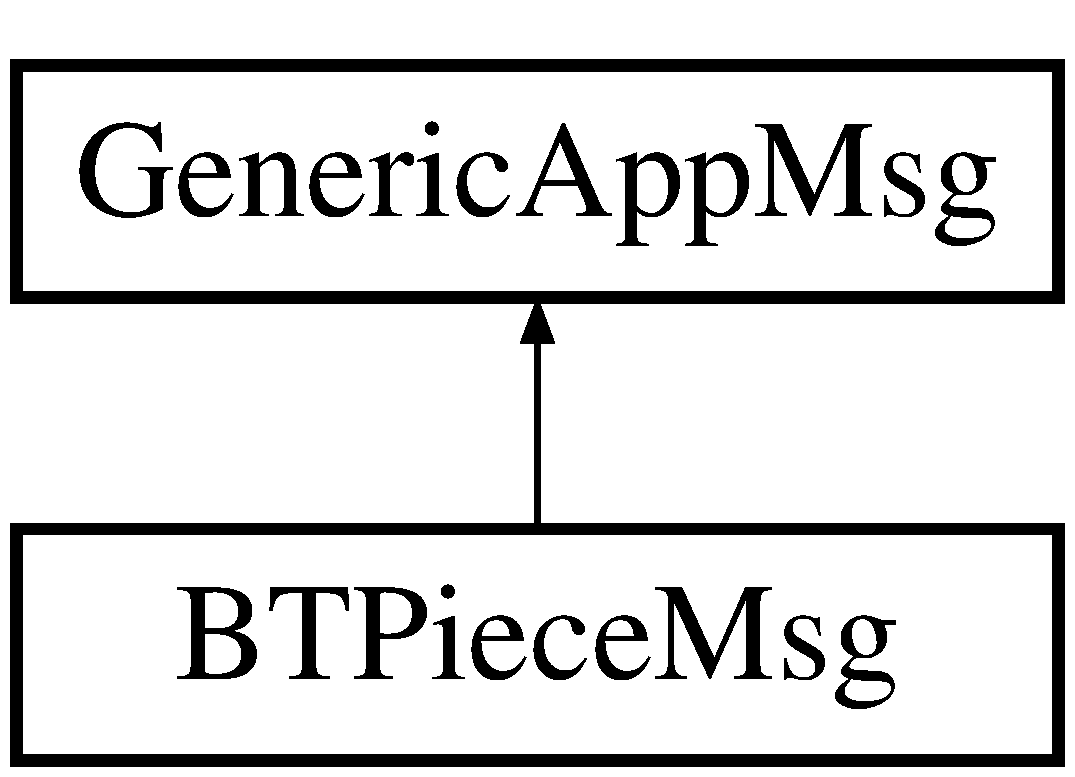
\includegraphics[height=2.000000cm]{classBTPieceMsg}
\end{center}
\end{figure}
\subsection*{Public Member Functions}
\begin{DoxyCompactItemize}
\item 
\hyperlink{classBTPieceMsg_aab94a7d9cecf74bbcb4d33c73621e79d}{B\+T\+Piece\+Msg} (const char $\ast$name=N\+U\+L\+L, int kind=0)
\item 
\hyperlink{classBTPieceMsg_ab48d04a29681a8811a4c6d89da094694}{B\+T\+Piece\+Msg} (const \hyperlink{classBTPieceMsg}{B\+T\+Piece\+Msg} \&other)
\item 
virtual \hyperlink{classBTPieceMsg_afd8e46d483a4b668ba2ddbb9ca590026}{$\sim$\+B\+T\+Piece\+Msg} ()
\item 
\hyperlink{classBTPieceMsg}{B\+T\+Piece\+Msg} \& \hyperlink{classBTPieceMsg_ac1bfbf0821b74bff9ba498d184e284f8}{operator=} (const \hyperlink{classBTPieceMsg}{B\+T\+Piece\+Msg} \&other)
\item 
virtual \hyperlink{classBTPieceMsg}{B\+T\+Piece\+Msg} $\ast$ \hyperlink{classBTPieceMsg_a8a9595f0d774d5ca06c7639429a93466}{dup} () const 
\item 
virtual void \hyperlink{classBTPieceMsg_a4c624dd2267836deb6779537738c492d}{parsim\+Pack} (c\+Comm\+Buffer $\ast$b)
\item 
virtual void \hyperlink{classBTPieceMsg_a8d1a9a3ac51eab276e6126dd4efece0a}{parsim\+Unpack} (c\+Comm\+Buffer $\ast$b)
\item 
virtual int \hyperlink{classBTPieceMsg_a18301230ce36b59e267b85187f44bafb}{length\+\_\+prefix} () const 
\item 
virtual void \hyperlink{classBTPieceMsg_a8b2686847a190f607d47a468a987ee39}{set\+Length\+\_\+prefix} (int \hyperlink{classBTPieceMsg_a003b938dabb53ea470ef14fee77ce17c}{length\+\_\+prefix\+\_\+var})
\item 
virtual unsigned short \hyperlink{classBTPieceMsg_a735d57e9641da83acaef1ae2d07b8a68}{I\+D} () const 
\item 
virtual void \hyperlink{classBTPieceMsg_a11ae1569ddf762680aea8080bc5ff3a8}{set\+I\+D} (unsigned short \hyperlink{classBTPieceMsg_aa46d6993c9d02a3b4add2a69b811de48}{I\+D\+\_\+var})
\item 
virtual int \hyperlink{classBTPieceMsg_ad88358d275933f9df950b6ce5d2b13f8}{index} () const 
\item 
virtual void \hyperlink{classBTPieceMsg_aabb09154f661b4f224b683be6d97148a}{set\+Index} (int \hyperlink{classBTPieceMsg_a5caacefaece64a71bc6b5e209e4d13a0}{index\+\_\+var})
\item 
virtual int \hyperlink{classBTPieceMsg_a2d78a296cd35afe5da527cc6f1866e80}{begin} () const 
\item 
virtual void \hyperlink{classBTPieceMsg_aa17191c3a4c9706e161294a223c15393}{set\+Begin} (int \hyperlink{classBTPieceMsg_a0d1fed26edc84d361d74986fa4593c71}{begin\+\_\+var})
\item 
virtual const char $\ast$ \hyperlink{classBTPieceMsg_a39e81e0d245415035f119c31dbc54723}{data} () const 
\item 
virtual void \hyperlink{classBTPieceMsg_aa0628ba79c3d9f027c0a64f8f58bd6bb}{set\+Data} (const char $\ast$\hyperlink{classBTPieceMsg_ab0ce35b2c10df0e33900776ce415473d}{data\+\_\+var})
\end{DoxyCompactItemize}
\subsection*{Protected Member Functions}
\begin{DoxyCompactItemize}
\item 
bool \hyperlink{classBTPieceMsg_a2a30af287383c392ef5abbc77a201b35}{operator==} (const \hyperlink{classBTPieceMsg}{B\+T\+Piece\+Msg} \&)
\end{DoxyCompactItemize}
\subsection*{Protected Attributes}
\begin{DoxyCompactItemize}
\item 
int \hyperlink{classBTPieceMsg_a003b938dabb53ea470ef14fee77ce17c}{length\+\_\+prefix\+\_\+var}
\item 
unsigned short \hyperlink{classBTPieceMsg_aa46d6993c9d02a3b4add2a69b811de48}{I\+D\+\_\+var}
\item 
int \hyperlink{classBTPieceMsg_a5caacefaece64a71bc6b5e209e4d13a0}{index\+\_\+var}
\item 
int \hyperlink{classBTPieceMsg_a0d1fed26edc84d361d74986fa4593c71}{begin\+\_\+var}
\item 
opp\+\_\+string \hyperlink{classBTPieceMsg_ab0ce35b2c10df0e33900776ce415473d}{data\+\_\+var}
\end{DoxyCompactItemize}


\subsection{Constructor \& Destructor Documentation}
\hypertarget{classBTPieceMsg_aab94a7d9cecf74bbcb4d33c73621e79d}{}\index{B\+T\+Piece\+Msg@{B\+T\+Piece\+Msg}!B\+T\+Piece\+Msg@{B\+T\+Piece\+Msg}}
\index{B\+T\+Piece\+Msg@{B\+T\+Piece\+Msg}!B\+T\+Piece\+Msg@{B\+T\+Piece\+Msg}}
\subsubsection[{B\+T\+Piece\+Msg(const char $\ast$name=\+N\+U\+L\+L, int kind=0)}]{\setlength{\rightskip}{0pt plus 5cm}B\+T\+Piece\+Msg\+::\+B\+T\+Piece\+Msg (
\begin{DoxyParamCaption}
\item[{const char $\ast$}]{name = {\ttfamily NULL}, }
\item[{int}]{kind = {\ttfamily 0}}
\end{DoxyParamCaption}
)}\label{classBTPieceMsg_aab94a7d9cecf74bbcb4d33c73621e79d}
\hypertarget{classBTPieceMsg_ab48d04a29681a8811a4c6d89da094694}{}\index{B\+T\+Piece\+Msg@{B\+T\+Piece\+Msg}!B\+T\+Piece\+Msg@{B\+T\+Piece\+Msg}}
\index{B\+T\+Piece\+Msg@{B\+T\+Piece\+Msg}!B\+T\+Piece\+Msg@{B\+T\+Piece\+Msg}}
\subsubsection[{B\+T\+Piece\+Msg(const B\+T\+Piece\+Msg \&other)}]{\setlength{\rightskip}{0pt plus 5cm}B\+T\+Piece\+Msg\+::\+B\+T\+Piece\+Msg (
\begin{DoxyParamCaption}
\item[{const {\bf B\+T\+Piece\+Msg} \&}]{other}
\end{DoxyParamCaption}
)}\label{classBTPieceMsg_ab48d04a29681a8811a4c6d89da094694}
\hypertarget{classBTPieceMsg_afd8e46d483a4b668ba2ddbb9ca590026}{}\index{B\+T\+Piece\+Msg@{B\+T\+Piece\+Msg}!````~B\+T\+Piece\+Msg@{$\sim$\+B\+T\+Piece\+Msg}}
\index{````~B\+T\+Piece\+Msg@{$\sim$\+B\+T\+Piece\+Msg}!B\+T\+Piece\+Msg@{B\+T\+Piece\+Msg}}
\subsubsection[{$\sim$\+B\+T\+Piece\+Msg()}]{\setlength{\rightskip}{0pt plus 5cm}B\+T\+Piece\+Msg\+::$\sim$\+B\+T\+Piece\+Msg (
\begin{DoxyParamCaption}
{}
\end{DoxyParamCaption}
)\hspace{0.3cm}{\ttfamily [virtual]}}\label{classBTPieceMsg_afd8e46d483a4b668ba2ddbb9ca590026}


\subsection{Member Function Documentation}
\hypertarget{classBTPieceMsg_a2d78a296cd35afe5da527cc6f1866e80}{}\index{B\+T\+Piece\+Msg@{B\+T\+Piece\+Msg}!begin@{begin}}
\index{begin@{begin}!B\+T\+Piece\+Msg@{B\+T\+Piece\+Msg}}
\subsubsection[{begin() const }]{\setlength{\rightskip}{0pt plus 5cm}int B\+T\+Piece\+Msg\+::begin (
\begin{DoxyParamCaption}
{}
\end{DoxyParamCaption}
) const\hspace{0.3cm}{\ttfamily [virtual]}}\label{classBTPieceMsg_a2d78a296cd35afe5da527cc6f1866e80}
\hypertarget{classBTPieceMsg_a39e81e0d245415035f119c31dbc54723}{}\index{B\+T\+Piece\+Msg@{B\+T\+Piece\+Msg}!data@{data}}
\index{data@{data}!B\+T\+Piece\+Msg@{B\+T\+Piece\+Msg}}
\subsubsection[{data() const }]{\setlength{\rightskip}{0pt plus 5cm}const char $\ast$ B\+T\+Piece\+Msg\+::data (
\begin{DoxyParamCaption}
{}
\end{DoxyParamCaption}
) const\hspace{0.3cm}{\ttfamily [virtual]}}\label{classBTPieceMsg_a39e81e0d245415035f119c31dbc54723}
\hypertarget{classBTPieceMsg_a8a9595f0d774d5ca06c7639429a93466}{}\index{B\+T\+Piece\+Msg@{B\+T\+Piece\+Msg}!dup@{dup}}
\index{dup@{dup}!B\+T\+Piece\+Msg@{B\+T\+Piece\+Msg}}
\subsubsection[{dup() const }]{\setlength{\rightskip}{0pt plus 5cm}virtual {\bf B\+T\+Piece\+Msg}$\ast$ B\+T\+Piece\+Msg\+::dup (
\begin{DoxyParamCaption}
{}
\end{DoxyParamCaption}
) const\hspace{0.3cm}{\ttfamily [inline]}, {\ttfamily [virtual]}}\label{classBTPieceMsg_a8a9595f0d774d5ca06c7639429a93466}
\hypertarget{classBTPieceMsg_a735d57e9641da83acaef1ae2d07b8a68}{}\index{B\+T\+Piece\+Msg@{B\+T\+Piece\+Msg}!I\+D@{I\+D}}
\index{I\+D@{I\+D}!B\+T\+Piece\+Msg@{B\+T\+Piece\+Msg}}
\subsubsection[{I\+D() const }]{\setlength{\rightskip}{0pt plus 5cm}unsigned short B\+T\+Piece\+Msg\+::\+I\+D (
\begin{DoxyParamCaption}
{}
\end{DoxyParamCaption}
) const\hspace{0.3cm}{\ttfamily [virtual]}}\label{classBTPieceMsg_a735d57e9641da83acaef1ae2d07b8a68}
\hypertarget{classBTPieceMsg_ad88358d275933f9df950b6ce5d2b13f8}{}\index{B\+T\+Piece\+Msg@{B\+T\+Piece\+Msg}!index@{index}}
\index{index@{index}!B\+T\+Piece\+Msg@{B\+T\+Piece\+Msg}}
\subsubsection[{index() const }]{\setlength{\rightskip}{0pt plus 5cm}int B\+T\+Piece\+Msg\+::index (
\begin{DoxyParamCaption}
{}
\end{DoxyParamCaption}
) const\hspace{0.3cm}{\ttfamily [virtual]}}\label{classBTPieceMsg_ad88358d275933f9df950b6ce5d2b13f8}
\hypertarget{classBTPieceMsg_a18301230ce36b59e267b85187f44bafb}{}\index{B\+T\+Piece\+Msg@{B\+T\+Piece\+Msg}!length\+\_\+prefix@{length\+\_\+prefix}}
\index{length\+\_\+prefix@{length\+\_\+prefix}!B\+T\+Piece\+Msg@{B\+T\+Piece\+Msg}}
\subsubsection[{length\+\_\+prefix() const }]{\setlength{\rightskip}{0pt plus 5cm}int B\+T\+Piece\+Msg\+::length\+\_\+prefix (
\begin{DoxyParamCaption}
{}
\end{DoxyParamCaption}
) const\hspace{0.3cm}{\ttfamily [virtual]}}\label{classBTPieceMsg_a18301230ce36b59e267b85187f44bafb}
\hypertarget{classBTPieceMsg_ac1bfbf0821b74bff9ba498d184e284f8}{}\index{B\+T\+Piece\+Msg@{B\+T\+Piece\+Msg}!operator=@{operator=}}
\index{operator=@{operator=}!B\+T\+Piece\+Msg@{B\+T\+Piece\+Msg}}
\subsubsection[{operator=(const B\+T\+Piece\+Msg \&other)}]{\setlength{\rightskip}{0pt plus 5cm}{\bf B\+T\+Piece\+Msg} \& B\+T\+Piece\+Msg\+::operator= (
\begin{DoxyParamCaption}
\item[{const {\bf B\+T\+Piece\+Msg} \&}]{other}
\end{DoxyParamCaption}
)}\label{classBTPieceMsg_ac1bfbf0821b74bff9ba498d184e284f8}
\hypertarget{classBTPieceMsg_a2a30af287383c392ef5abbc77a201b35}{}\index{B\+T\+Piece\+Msg@{B\+T\+Piece\+Msg}!operator==@{operator==}}
\index{operator==@{operator==}!B\+T\+Piece\+Msg@{B\+T\+Piece\+Msg}}
\subsubsection[{operator==(const B\+T\+Piece\+Msg \&)}]{\setlength{\rightskip}{0pt plus 5cm}bool B\+T\+Piece\+Msg\+::operator== (
\begin{DoxyParamCaption}
\item[{const {\bf B\+T\+Piece\+Msg} \&}]{}
\end{DoxyParamCaption}
)\hspace{0.3cm}{\ttfamily [protected]}}\label{classBTPieceMsg_a2a30af287383c392ef5abbc77a201b35}
\hypertarget{classBTPieceMsg_a4c624dd2267836deb6779537738c492d}{}\index{B\+T\+Piece\+Msg@{B\+T\+Piece\+Msg}!parsim\+Pack@{parsim\+Pack}}
\index{parsim\+Pack@{parsim\+Pack}!B\+T\+Piece\+Msg@{B\+T\+Piece\+Msg}}
\subsubsection[{parsim\+Pack(c\+Comm\+Buffer $\ast$b)}]{\setlength{\rightskip}{0pt plus 5cm}void B\+T\+Piece\+Msg\+::parsim\+Pack (
\begin{DoxyParamCaption}
\item[{c\+Comm\+Buffer $\ast$}]{b}
\end{DoxyParamCaption}
)\hspace{0.3cm}{\ttfamily [virtual]}}\label{classBTPieceMsg_a4c624dd2267836deb6779537738c492d}
\hypertarget{classBTPieceMsg_a8d1a9a3ac51eab276e6126dd4efece0a}{}\index{B\+T\+Piece\+Msg@{B\+T\+Piece\+Msg}!parsim\+Unpack@{parsim\+Unpack}}
\index{parsim\+Unpack@{parsim\+Unpack}!B\+T\+Piece\+Msg@{B\+T\+Piece\+Msg}}
\subsubsection[{parsim\+Unpack(c\+Comm\+Buffer $\ast$b)}]{\setlength{\rightskip}{0pt plus 5cm}void B\+T\+Piece\+Msg\+::parsim\+Unpack (
\begin{DoxyParamCaption}
\item[{c\+Comm\+Buffer $\ast$}]{b}
\end{DoxyParamCaption}
)\hspace{0.3cm}{\ttfamily [virtual]}}\label{classBTPieceMsg_a8d1a9a3ac51eab276e6126dd4efece0a}
\hypertarget{classBTPieceMsg_aa17191c3a4c9706e161294a223c15393}{}\index{B\+T\+Piece\+Msg@{B\+T\+Piece\+Msg}!set\+Begin@{set\+Begin}}
\index{set\+Begin@{set\+Begin}!B\+T\+Piece\+Msg@{B\+T\+Piece\+Msg}}
\subsubsection[{set\+Begin(int begin\+\_\+var)}]{\setlength{\rightskip}{0pt plus 5cm}void B\+T\+Piece\+Msg\+::set\+Begin (
\begin{DoxyParamCaption}
\item[{int}]{begin\+\_\+var}
\end{DoxyParamCaption}
)\hspace{0.3cm}{\ttfamily [virtual]}}\label{classBTPieceMsg_aa17191c3a4c9706e161294a223c15393}
\hypertarget{classBTPieceMsg_aa0628ba79c3d9f027c0a64f8f58bd6bb}{}\index{B\+T\+Piece\+Msg@{B\+T\+Piece\+Msg}!set\+Data@{set\+Data}}
\index{set\+Data@{set\+Data}!B\+T\+Piece\+Msg@{B\+T\+Piece\+Msg}}
\subsubsection[{set\+Data(const char $\ast$data\+\_\+var)}]{\setlength{\rightskip}{0pt plus 5cm}void B\+T\+Piece\+Msg\+::set\+Data (
\begin{DoxyParamCaption}
\item[{const char $\ast$}]{data\+\_\+var}
\end{DoxyParamCaption}
)\hspace{0.3cm}{\ttfamily [virtual]}}\label{classBTPieceMsg_aa0628ba79c3d9f027c0a64f8f58bd6bb}
\hypertarget{classBTPieceMsg_a11ae1569ddf762680aea8080bc5ff3a8}{}\index{B\+T\+Piece\+Msg@{B\+T\+Piece\+Msg}!set\+I\+D@{set\+I\+D}}
\index{set\+I\+D@{set\+I\+D}!B\+T\+Piece\+Msg@{B\+T\+Piece\+Msg}}
\subsubsection[{set\+I\+D(unsigned short I\+D\+\_\+var)}]{\setlength{\rightskip}{0pt plus 5cm}void B\+T\+Piece\+Msg\+::set\+I\+D (
\begin{DoxyParamCaption}
\item[{unsigned short}]{I\+D\+\_\+var}
\end{DoxyParamCaption}
)\hspace{0.3cm}{\ttfamily [virtual]}}\label{classBTPieceMsg_a11ae1569ddf762680aea8080bc5ff3a8}
\hypertarget{classBTPieceMsg_aabb09154f661b4f224b683be6d97148a}{}\index{B\+T\+Piece\+Msg@{B\+T\+Piece\+Msg}!set\+Index@{set\+Index}}
\index{set\+Index@{set\+Index}!B\+T\+Piece\+Msg@{B\+T\+Piece\+Msg}}
\subsubsection[{set\+Index(int index\+\_\+var)}]{\setlength{\rightskip}{0pt plus 5cm}void B\+T\+Piece\+Msg\+::set\+Index (
\begin{DoxyParamCaption}
\item[{int}]{index\+\_\+var}
\end{DoxyParamCaption}
)\hspace{0.3cm}{\ttfamily [virtual]}}\label{classBTPieceMsg_aabb09154f661b4f224b683be6d97148a}
\hypertarget{classBTPieceMsg_a8b2686847a190f607d47a468a987ee39}{}\index{B\+T\+Piece\+Msg@{B\+T\+Piece\+Msg}!set\+Length\+\_\+prefix@{set\+Length\+\_\+prefix}}
\index{set\+Length\+\_\+prefix@{set\+Length\+\_\+prefix}!B\+T\+Piece\+Msg@{B\+T\+Piece\+Msg}}
\subsubsection[{set\+Length\+\_\+prefix(int length\+\_\+prefix\+\_\+var)}]{\setlength{\rightskip}{0pt plus 5cm}void B\+T\+Piece\+Msg\+::set\+Length\+\_\+prefix (
\begin{DoxyParamCaption}
\item[{int}]{length\+\_\+prefix\+\_\+var}
\end{DoxyParamCaption}
)\hspace{0.3cm}{\ttfamily [virtual]}}\label{classBTPieceMsg_a8b2686847a190f607d47a468a987ee39}


\subsection{Member Data Documentation}
\hypertarget{classBTPieceMsg_a0d1fed26edc84d361d74986fa4593c71}{}\index{B\+T\+Piece\+Msg@{B\+T\+Piece\+Msg}!begin\+\_\+var@{begin\+\_\+var}}
\index{begin\+\_\+var@{begin\+\_\+var}!B\+T\+Piece\+Msg@{B\+T\+Piece\+Msg}}
\subsubsection[{begin\+\_\+var}]{\setlength{\rightskip}{0pt plus 5cm}int B\+T\+Piece\+Msg\+::begin\+\_\+var\hspace{0.3cm}{\ttfamily [protected]}}\label{classBTPieceMsg_a0d1fed26edc84d361d74986fa4593c71}
\hypertarget{classBTPieceMsg_ab0ce35b2c10df0e33900776ce415473d}{}\index{B\+T\+Piece\+Msg@{B\+T\+Piece\+Msg}!data\+\_\+var@{data\+\_\+var}}
\index{data\+\_\+var@{data\+\_\+var}!B\+T\+Piece\+Msg@{B\+T\+Piece\+Msg}}
\subsubsection[{data\+\_\+var}]{\setlength{\rightskip}{0pt plus 5cm}opp\+\_\+string B\+T\+Piece\+Msg\+::data\+\_\+var\hspace{0.3cm}{\ttfamily [protected]}}\label{classBTPieceMsg_ab0ce35b2c10df0e33900776ce415473d}
\hypertarget{classBTPieceMsg_aa46d6993c9d02a3b4add2a69b811de48}{}\index{B\+T\+Piece\+Msg@{B\+T\+Piece\+Msg}!I\+D\+\_\+var@{I\+D\+\_\+var}}
\index{I\+D\+\_\+var@{I\+D\+\_\+var}!B\+T\+Piece\+Msg@{B\+T\+Piece\+Msg}}
\subsubsection[{I\+D\+\_\+var}]{\setlength{\rightskip}{0pt plus 5cm}unsigned short B\+T\+Piece\+Msg\+::\+I\+D\+\_\+var\hspace{0.3cm}{\ttfamily [protected]}}\label{classBTPieceMsg_aa46d6993c9d02a3b4add2a69b811de48}
\hypertarget{classBTPieceMsg_a5caacefaece64a71bc6b5e209e4d13a0}{}\index{B\+T\+Piece\+Msg@{B\+T\+Piece\+Msg}!index\+\_\+var@{index\+\_\+var}}
\index{index\+\_\+var@{index\+\_\+var}!B\+T\+Piece\+Msg@{B\+T\+Piece\+Msg}}
\subsubsection[{index\+\_\+var}]{\setlength{\rightskip}{0pt plus 5cm}int B\+T\+Piece\+Msg\+::index\+\_\+var\hspace{0.3cm}{\ttfamily [protected]}}\label{classBTPieceMsg_a5caacefaece64a71bc6b5e209e4d13a0}
\hypertarget{classBTPieceMsg_a003b938dabb53ea470ef14fee77ce17c}{}\index{B\+T\+Piece\+Msg@{B\+T\+Piece\+Msg}!length\+\_\+prefix\+\_\+var@{length\+\_\+prefix\+\_\+var}}
\index{length\+\_\+prefix\+\_\+var@{length\+\_\+prefix\+\_\+var}!B\+T\+Piece\+Msg@{B\+T\+Piece\+Msg}}
\subsubsection[{length\+\_\+prefix\+\_\+var}]{\setlength{\rightskip}{0pt plus 5cm}int B\+T\+Piece\+Msg\+::length\+\_\+prefix\+\_\+var\hspace{0.3cm}{\ttfamily [protected]}}\label{classBTPieceMsg_a003b938dabb53ea470ef14fee77ce17c}


The documentation for this class was generated from the following files\+:\begin{DoxyCompactItemize}
\item 
\hyperlink{BTPeerWireMsg__m_8h}{B\+T\+Peer\+Wire\+Msg\+\_\+m.\+h}\item 
\hyperlink{BTPeerWireMsg__m_8cc}{B\+T\+Peer\+Wire\+Msg\+\_\+m.\+cc}\end{DoxyCompactItemize}

\hypertarget{classBTPieceMsgDescriptor}{}\section{B\+T\+Piece\+Msg\+Descriptor Class Reference}
\label{classBTPieceMsgDescriptor}\index{B\+T\+Piece\+Msg\+Descriptor@{B\+T\+Piece\+Msg\+Descriptor}}
Inheritance diagram for B\+T\+Piece\+Msg\+Descriptor\+:\begin{figure}[H]
\begin{center}
\leavevmode
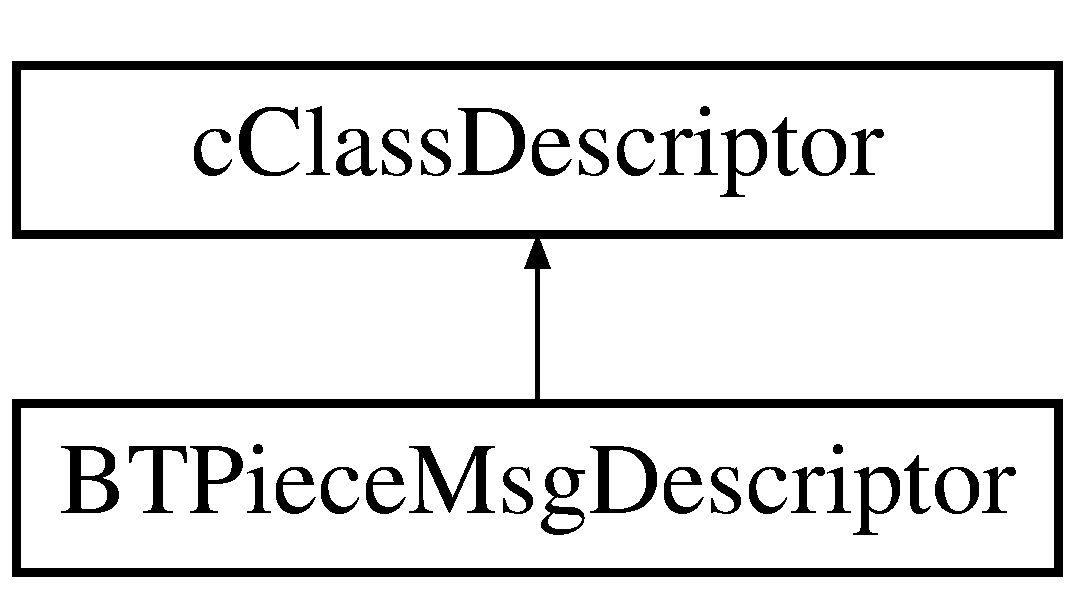
\includegraphics[height=2.000000cm]{classBTPieceMsgDescriptor}
\end{center}
\end{figure}
\subsection*{Public Member Functions}
\begin{DoxyCompactItemize}
\item 
\hyperlink{classBTPieceMsgDescriptor_ae84cd0e4aff65353a9124aee15876be8}{B\+T\+Piece\+Msg\+Descriptor} ()
\item 
virtual \hyperlink{classBTPieceMsgDescriptor_abee9379ba36c2c8cb930dc1ff9d05238}{$\sim$\+B\+T\+Piece\+Msg\+Descriptor} ()
\item 
virtual bool \hyperlink{classBTPieceMsgDescriptor_a59a58763b2753bc4e1f0e986a546fde2}{does\+Support} (c\+Object $\ast$obj) const 
\item 
virtual const char $\ast$ \hyperlink{classBTPieceMsgDescriptor_aa153a7a47256913d4fe69930aeae7462}{get\+Property} (const char $\ast$propertyname) const 
\item 
virtual int \hyperlink{classBTPieceMsgDescriptor_a641b734a4a3bc62caaa6ebaab49b2094}{get\+Field\+Count} (void $\ast$object) const 
\item 
virtual const char $\ast$ \hyperlink{classBTPieceMsgDescriptor_af00965c5ab3b862e6d58c70aea43ea8a}{get\+Field\+Name} (void $\ast$object, int field) const 
\item 
virtual int \hyperlink{classBTPieceMsgDescriptor_a460c1ad87acf58088cbc820846750565}{find\+Field} (void $\ast$object, const char $\ast$field\+Name) const 
\item 
virtual unsigned int \hyperlink{classBTPieceMsgDescriptor_a5c482406d825929f1878ec22b781e9b2}{get\+Field\+Type\+Flags} (void $\ast$object, int field) const 
\item 
virtual const char $\ast$ \hyperlink{classBTPieceMsgDescriptor_af000de1ab6182695034aeb0fb6fdfa0a}{get\+Field\+Type\+String} (void $\ast$object, int field) const 
\item 
virtual const char $\ast$ \hyperlink{classBTPieceMsgDescriptor_afd666218833cd580b45be5e05c435dea}{get\+Field\+Property} (void $\ast$object, int field, const char $\ast$propertyname) const 
\item 
virtual int \hyperlink{classBTPieceMsgDescriptor_a6e4a8fadd723fab1b3077d27a32deeca}{get\+Array\+Size} (void $\ast$object, int field) const 
\item 
virtual std\+::string \hyperlink{classBTPieceMsgDescriptor_a2790505d6b2ee409573346e135b06e9b}{get\+Field\+As\+String} (void $\ast$object, int field, int i) const 
\item 
virtual bool \hyperlink{classBTPieceMsgDescriptor_a9615195a8841c118b13d378e4d0a8f7f}{set\+Field\+As\+String} (void $\ast$object, int field, int i, const char $\ast$value) const 
\item 
virtual const char $\ast$ \hyperlink{classBTPieceMsgDescriptor_a6e2aa3f4ec5e540bf43f4e277e7c3d79}{get\+Field\+Struct\+Name} (void $\ast$object, int field) const 
\item 
virtual void $\ast$ \hyperlink{classBTPieceMsgDescriptor_a7ed387291492374f2bea1b1f58597d83}{get\+Field\+Struct\+Pointer} (void $\ast$object, int field, int i) const 
\end{DoxyCompactItemize}


\subsection{Constructor \& Destructor Documentation}
\hypertarget{classBTPieceMsgDescriptor_ae84cd0e4aff65353a9124aee15876be8}{}\index{B\+T\+Piece\+Msg\+Descriptor@{B\+T\+Piece\+Msg\+Descriptor}!B\+T\+Piece\+Msg\+Descriptor@{B\+T\+Piece\+Msg\+Descriptor}}
\index{B\+T\+Piece\+Msg\+Descriptor@{B\+T\+Piece\+Msg\+Descriptor}!B\+T\+Piece\+Msg\+Descriptor@{B\+T\+Piece\+Msg\+Descriptor}}
\subsubsection[{B\+T\+Piece\+Msg\+Descriptor()}]{\setlength{\rightskip}{0pt plus 5cm}B\+T\+Piece\+Msg\+Descriptor\+::\+B\+T\+Piece\+Msg\+Descriptor (
\begin{DoxyParamCaption}
{}
\end{DoxyParamCaption}
)}\label{classBTPieceMsgDescriptor_ae84cd0e4aff65353a9124aee15876be8}
\hypertarget{classBTPieceMsgDescriptor_abee9379ba36c2c8cb930dc1ff9d05238}{}\index{B\+T\+Piece\+Msg\+Descriptor@{B\+T\+Piece\+Msg\+Descriptor}!````~B\+T\+Piece\+Msg\+Descriptor@{$\sim$\+B\+T\+Piece\+Msg\+Descriptor}}
\index{````~B\+T\+Piece\+Msg\+Descriptor@{$\sim$\+B\+T\+Piece\+Msg\+Descriptor}!B\+T\+Piece\+Msg\+Descriptor@{B\+T\+Piece\+Msg\+Descriptor}}
\subsubsection[{$\sim$\+B\+T\+Piece\+Msg\+Descriptor()}]{\setlength{\rightskip}{0pt plus 5cm}B\+T\+Piece\+Msg\+Descriptor\+::$\sim$\+B\+T\+Piece\+Msg\+Descriptor (
\begin{DoxyParamCaption}
{}
\end{DoxyParamCaption}
)\hspace{0.3cm}{\ttfamily [virtual]}}\label{classBTPieceMsgDescriptor_abee9379ba36c2c8cb930dc1ff9d05238}


\subsection{Member Function Documentation}
\hypertarget{classBTPieceMsgDescriptor_a59a58763b2753bc4e1f0e986a546fde2}{}\index{B\+T\+Piece\+Msg\+Descriptor@{B\+T\+Piece\+Msg\+Descriptor}!does\+Support@{does\+Support}}
\index{does\+Support@{does\+Support}!B\+T\+Piece\+Msg\+Descriptor@{B\+T\+Piece\+Msg\+Descriptor}}
\subsubsection[{does\+Support(c\+Object $\ast$obj) const }]{\setlength{\rightskip}{0pt plus 5cm}bool B\+T\+Piece\+Msg\+Descriptor\+::does\+Support (
\begin{DoxyParamCaption}
\item[{c\+Object $\ast$}]{obj}
\end{DoxyParamCaption}
) const\hspace{0.3cm}{\ttfamily [virtual]}}\label{classBTPieceMsgDescriptor_a59a58763b2753bc4e1f0e986a546fde2}
\hypertarget{classBTPieceMsgDescriptor_a460c1ad87acf58088cbc820846750565}{}\index{B\+T\+Piece\+Msg\+Descriptor@{B\+T\+Piece\+Msg\+Descriptor}!find\+Field@{find\+Field}}
\index{find\+Field@{find\+Field}!B\+T\+Piece\+Msg\+Descriptor@{B\+T\+Piece\+Msg\+Descriptor}}
\subsubsection[{find\+Field(void $\ast$object, const char $\ast$field\+Name) const }]{\setlength{\rightskip}{0pt plus 5cm}int B\+T\+Piece\+Msg\+Descriptor\+::find\+Field (
\begin{DoxyParamCaption}
\item[{void $\ast$}]{object, }
\item[{const char $\ast$}]{field\+Name}
\end{DoxyParamCaption}
) const\hspace{0.3cm}{\ttfamily [virtual]}}\label{classBTPieceMsgDescriptor_a460c1ad87acf58088cbc820846750565}
\hypertarget{classBTPieceMsgDescriptor_a6e4a8fadd723fab1b3077d27a32deeca}{}\index{B\+T\+Piece\+Msg\+Descriptor@{B\+T\+Piece\+Msg\+Descriptor}!get\+Array\+Size@{get\+Array\+Size}}
\index{get\+Array\+Size@{get\+Array\+Size}!B\+T\+Piece\+Msg\+Descriptor@{B\+T\+Piece\+Msg\+Descriptor}}
\subsubsection[{get\+Array\+Size(void $\ast$object, int field) const }]{\setlength{\rightskip}{0pt plus 5cm}int B\+T\+Piece\+Msg\+Descriptor\+::get\+Array\+Size (
\begin{DoxyParamCaption}
\item[{void $\ast$}]{object, }
\item[{int}]{field}
\end{DoxyParamCaption}
) const\hspace{0.3cm}{\ttfamily [virtual]}}\label{classBTPieceMsgDescriptor_a6e4a8fadd723fab1b3077d27a32deeca}
\hypertarget{classBTPieceMsgDescriptor_a2790505d6b2ee409573346e135b06e9b}{}\index{B\+T\+Piece\+Msg\+Descriptor@{B\+T\+Piece\+Msg\+Descriptor}!get\+Field\+As\+String@{get\+Field\+As\+String}}
\index{get\+Field\+As\+String@{get\+Field\+As\+String}!B\+T\+Piece\+Msg\+Descriptor@{B\+T\+Piece\+Msg\+Descriptor}}
\subsubsection[{get\+Field\+As\+String(void $\ast$object, int field, int i) const }]{\setlength{\rightskip}{0pt plus 5cm}std\+::string B\+T\+Piece\+Msg\+Descriptor\+::get\+Field\+As\+String (
\begin{DoxyParamCaption}
\item[{void $\ast$}]{object, }
\item[{int}]{field, }
\item[{int}]{i}
\end{DoxyParamCaption}
) const\hspace{0.3cm}{\ttfamily [virtual]}}\label{classBTPieceMsgDescriptor_a2790505d6b2ee409573346e135b06e9b}
\hypertarget{classBTPieceMsgDescriptor_a641b734a4a3bc62caaa6ebaab49b2094}{}\index{B\+T\+Piece\+Msg\+Descriptor@{B\+T\+Piece\+Msg\+Descriptor}!get\+Field\+Count@{get\+Field\+Count}}
\index{get\+Field\+Count@{get\+Field\+Count}!B\+T\+Piece\+Msg\+Descriptor@{B\+T\+Piece\+Msg\+Descriptor}}
\subsubsection[{get\+Field\+Count(void $\ast$object) const }]{\setlength{\rightskip}{0pt plus 5cm}int B\+T\+Piece\+Msg\+Descriptor\+::get\+Field\+Count (
\begin{DoxyParamCaption}
\item[{void $\ast$}]{object}
\end{DoxyParamCaption}
) const\hspace{0.3cm}{\ttfamily [virtual]}}\label{classBTPieceMsgDescriptor_a641b734a4a3bc62caaa6ebaab49b2094}
\hypertarget{classBTPieceMsgDescriptor_af00965c5ab3b862e6d58c70aea43ea8a}{}\index{B\+T\+Piece\+Msg\+Descriptor@{B\+T\+Piece\+Msg\+Descriptor}!get\+Field\+Name@{get\+Field\+Name}}
\index{get\+Field\+Name@{get\+Field\+Name}!B\+T\+Piece\+Msg\+Descriptor@{B\+T\+Piece\+Msg\+Descriptor}}
\subsubsection[{get\+Field\+Name(void $\ast$object, int field) const }]{\setlength{\rightskip}{0pt plus 5cm}const char $\ast$ B\+T\+Piece\+Msg\+Descriptor\+::get\+Field\+Name (
\begin{DoxyParamCaption}
\item[{void $\ast$}]{object, }
\item[{int}]{field}
\end{DoxyParamCaption}
) const\hspace{0.3cm}{\ttfamily [virtual]}}\label{classBTPieceMsgDescriptor_af00965c5ab3b862e6d58c70aea43ea8a}
\hypertarget{classBTPieceMsgDescriptor_afd666218833cd580b45be5e05c435dea}{}\index{B\+T\+Piece\+Msg\+Descriptor@{B\+T\+Piece\+Msg\+Descriptor}!get\+Field\+Property@{get\+Field\+Property}}
\index{get\+Field\+Property@{get\+Field\+Property}!B\+T\+Piece\+Msg\+Descriptor@{B\+T\+Piece\+Msg\+Descriptor}}
\subsubsection[{get\+Field\+Property(void $\ast$object, int field, const char $\ast$propertyname) const }]{\setlength{\rightskip}{0pt plus 5cm}const char $\ast$ B\+T\+Piece\+Msg\+Descriptor\+::get\+Field\+Property (
\begin{DoxyParamCaption}
\item[{void $\ast$}]{object, }
\item[{int}]{field, }
\item[{const char $\ast$}]{propertyname}
\end{DoxyParamCaption}
) const\hspace{0.3cm}{\ttfamily [virtual]}}\label{classBTPieceMsgDescriptor_afd666218833cd580b45be5e05c435dea}
\hypertarget{classBTPieceMsgDescriptor_a6e2aa3f4ec5e540bf43f4e277e7c3d79}{}\index{B\+T\+Piece\+Msg\+Descriptor@{B\+T\+Piece\+Msg\+Descriptor}!get\+Field\+Struct\+Name@{get\+Field\+Struct\+Name}}
\index{get\+Field\+Struct\+Name@{get\+Field\+Struct\+Name}!B\+T\+Piece\+Msg\+Descriptor@{B\+T\+Piece\+Msg\+Descriptor}}
\subsubsection[{get\+Field\+Struct\+Name(void $\ast$object, int field) const }]{\setlength{\rightskip}{0pt plus 5cm}const char $\ast$ B\+T\+Piece\+Msg\+Descriptor\+::get\+Field\+Struct\+Name (
\begin{DoxyParamCaption}
\item[{void $\ast$}]{object, }
\item[{int}]{field}
\end{DoxyParamCaption}
) const\hspace{0.3cm}{\ttfamily [virtual]}}\label{classBTPieceMsgDescriptor_a6e2aa3f4ec5e540bf43f4e277e7c3d79}
\hypertarget{classBTPieceMsgDescriptor_a7ed387291492374f2bea1b1f58597d83}{}\index{B\+T\+Piece\+Msg\+Descriptor@{B\+T\+Piece\+Msg\+Descriptor}!get\+Field\+Struct\+Pointer@{get\+Field\+Struct\+Pointer}}
\index{get\+Field\+Struct\+Pointer@{get\+Field\+Struct\+Pointer}!B\+T\+Piece\+Msg\+Descriptor@{B\+T\+Piece\+Msg\+Descriptor}}
\subsubsection[{get\+Field\+Struct\+Pointer(void $\ast$object, int field, int i) const }]{\setlength{\rightskip}{0pt plus 5cm}void $\ast$ B\+T\+Piece\+Msg\+Descriptor\+::get\+Field\+Struct\+Pointer (
\begin{DoxyParamCaption}
\item[{void $\ast$}]{object, }
\item[{int}]{field, }
\item[{int}]{i}
\end{DoxyParamCaption}
) const\hspace{0.3cm}{\ttfamily [virtual]}}\label{classBTPieceMsgDescriptor_a7ed387291492374f2bea1b1f58597d83}
\hypertarget{classBTPieceMsgDescriptor_a5c482406d825929f1878ec22b781e9b2}{}\index{B\+T\+Piece\+Msg\+Descriptor@{B\+T\+Piece\+Msg\+Descriptor}!get\+Field\+Type\+Flags@{get\+Field\+Type\+Flags}}
\index{get\+Field\+Type\+Flags@{get\+Field\+Type\+Flags}!B\+T\+Piece\+Msg\+Descriptor@{B\+T\+Piece\+Msg\+Descriptor}}
\subsubsection[{get\+Field\+Type\+Flags(void $\ast$object, int field) const }]{\setlength{\rightskip}{0pt plus 5cm}unsigned int B\+T\+Piece\+Msg\+Descriptor\+::get\+Field\+Type\+Flags (
\begin{DoxyParamCaption}
\item[{void $\ast$}]{object, }
\item[{int}]{field}
\end{DoxyParamCaption}
) const\hspace{0.3cm}{\ttfamily [virtual]}}\label{classBTPieceMsgDescriptor_a5c482406d825929f1878ec22b781e9b2}
\hypertarget{classBTPieceMsgDescriptor_af000de1ab6182695034aeb0fb6fdfa0a}{}\index{B\+T\+Piece\+Msg\+Descriptor@{B\+T\+Piece\+Msg\+Descriptor}!get\+Field\+Type\+String@{get\+Field\+Type\+String}}
\index{get\+Field\+Type\+String@{get\+Field\+Type\+String}!B\+T\+Piece\+Msg\+Descriptor@{B\+T\+Piece\+Msg\+Descriptor}}
\subsubsection[{get\+Field\+Type\+String(void $\ast$object, int field) const }]{\setlength{\rightskip}{0pt plus 5cm}const char $\ast$ B\+T\+Piece\+Msg\+Descriptor\+::get\+Field\+Type\+String (
\begin{DoxyParamCaption}
\item[{void $\ast$}]{object, }
\item[{int}]{field}
\end{DoxyParamCaption}
) const\hspace{0.3cm}{\ttfamily [virtual]}}\label{classBTPieceMsgDescriptor_af000de1ab6182695034aeb0fb6fdfa0a}
\hypertarget{classBTPieceMsgDescriptor_aa153a7a47256913d4fe69930aeae7462}{}\index{B\+T\+Piece\+Msg\+Descriptor@{B\+T\+Piece\+Msg\+Descriptor}!get\+Property@{get\+Property}}
\index{get\+Property@{get\+Property}!B\+T\+Piece\+Msg\+Descriptor@{B\+T\+Piece\+Msg\+Descriptor}}
\subsubsection[{get\+Property(const char $\ast$propertyname) const }]{\setlength{\rightskip}{0pt plus 5cm}const char $\ast$ B\+T\+Piece\+Msg\+Descriptor\+::get\+Property (
\begin{DoxyParamCaption}
\item[{const char $\ast$}]{propertyname}
\end{DoxyParamCaption}
) const\hspace{0.3cm}{\ttfamily [virtual]}}\label{classBTPieceMsgDescriptor_aa153a7a47256913d4fe69930aeae7462}
\hypertarget{classBTPieceMsgDescriptor_a9615195a8841c118b13d378e4d0a8f7f}{}\index{B\+T\+Piece\+Msg\+Descriptor@{B\+T\+Piece\+Msg\+Descriptor}!set\+Field\+As\+String@{set\+Field\+As\+String}}
\index{set\+Field\+As\+String@{set\+Field\+As\+String}!B\+T\+Piece\+Msg\+Descriptor@{B\+T\+Piece\+Msg\+Descriptor}}
\subsubsection[{set\+Field\+As\+String(void $\ast$object, int field, int i, const char $\ast$value) const }]{\setlength{\rightskip}{0pt plus 5cm}bool B\+T\+Piece\+Msg\+Descriptor\+::set\+Field\+As\+String (
\begin{DoxyParamCaption}
\item[{void $\ast$}]{object, }
\item[{int}]{field, }
\item[{int}]{i, }
\item[{const char $\ast$}]{value}
\end{DoxyParamCaption}
) const\hspace{0.3cm}{\ttfamily [virtual]}}\label{classBTPieceMsgDescriptor_a9615195a8841c118b13d378e4d0a8f7f}


The documentation for this class was generated from the following file\+:\begin{DoxyCompactItemize}
\item 
\hyperlink{BTPeerWireMsg__m_8cc}{B\+T\+Peer\+Wire\+Msg\+\_\+m.\+cc}\end{DoxyCompactItemize}

\hypertarget{classBTRequestCancelMsg}{}\section{B\+T\+Request\+Cancel\+Msg Class Reference}
\label{classBTRequestCancelMsg}\index{B\+T\+Request\+Cancel\+Msg@{B\+T\+Request\+Cancel\+Msg}}


{\ttfamily \#include $<$B\+T\+Peer\+Wire\+Msg\+\_\+m.\+h$>$}

Inheritance diagram for B\+T\+Request\+Cancel\+Msg\+:\begin{figure}[H]
\begin{center}
\leavevmode
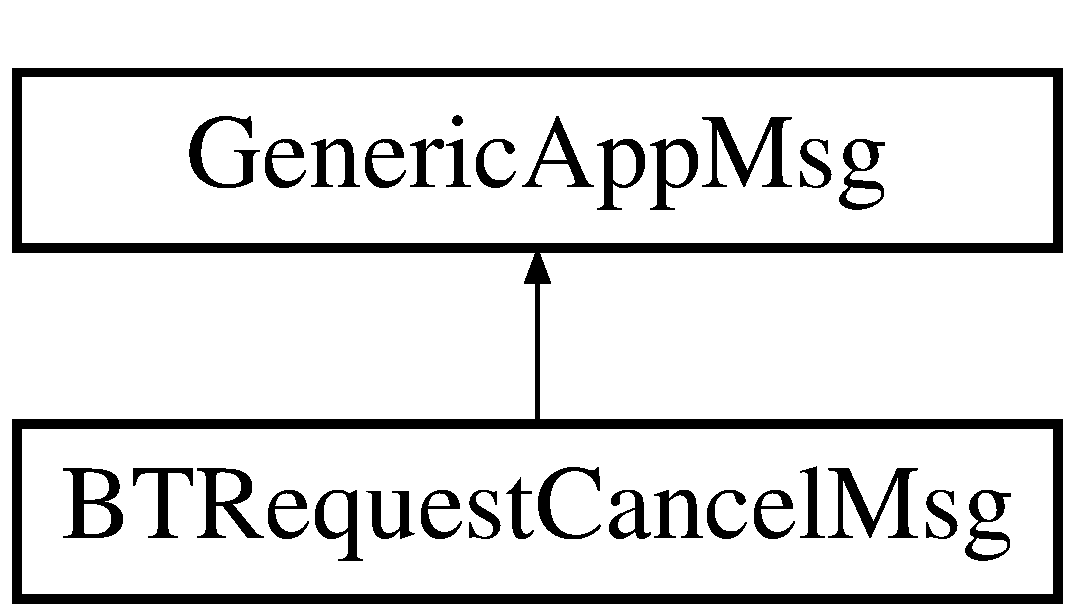
\includegraphics[height=2.000000cm]{classBTRequestCancelMsg}
\end{center}
\end{figure}
\subsection*{Public Member Functions}
\begin{DoxyCompactItemize}
\item 
\hyperlink{classBTRequestCancelMsg_a63ef83784a120293773ac59697413a0c}{B\+T\+Request\+Cancel\+Msg} (const char $\ast$name=N\+U\+L\+L, int kind=0)
\item 
\hyperlink{classBTRequestCancelMsg_a07eda41c73ff72f053e797c5711e65ac}{B\+T\+Request\+Cancel\+Msg} (const \hyperlink{classBTRequestCancelMsg}{B\+T\+Request\+Cancel\+Msg} \&other)
\item 
virtual \hyperlink{classBTRequestCancelMsg_a44fcdc94b3a53e3cb9843c9f983c964b}{$\sim$\+B\+T\+Request\+Cancel\+Msg} ()
\item 
\hyperlink{classBTRequestCancelMsg}{B\+T\+Request\+Cancel\+Msg} \& \hyperlink{classBTRequestCancelMsg_ad4865217b238706162fccbe7a8c332df}{operator=} (const \hyperlink{classBTRequestCancelMsg}{B\+T\+Request\+Cancel\+Msg} \&other)
\item 
virtual \hyperlink{classBTRequestCancelMsg}{B\+T\+Request\+Cancel\+Msg} $\ast$ \hyperlink{classBTRequestCancelMsg_ae5251077dad8b83275d516aae93bc605}{dup} () const 
\item 
virtual void \hyperlink{classBTRequestCancelMsg_a8256b2ec06d824e9afd63e304d349560}{parsim\+Pack} (c\+Comm\+Buffer $\ast$b)
\item 
virtual void \hyperlink{classBTRequestCancelMsg_a8bbbabcae9b44f7057c129b5adeb91b9}{parsim\+Unpack} (c\+Comm\+Buffer $\ast$b)
\item 
virtual int \hyperlink{classBTRequestCancelMsg_ad480f362891a35e93456d10fe7835662}{length\+\_\+prefix} () const 
\item 
virtual void \hyperlink{classBTRequestCancelMsg_a2d8e7794ff4441e3bdaaea0fb1b90916}{set\+Length\+\_\+prefix} (int \hyperlink{classBTRequestCancelMsg_a77139c7bdc2e1a7885f20ddbb25acf5d}{length\+\_\+prefix\+\_\+var})
\item 
virtual unsigned short \hyperlink{classBTRequestCancelMsg_ac4d90a27ad01b08fb4e8c72e73bb9230}{I\+D} () const 
\item 
virtual void \hyperlink{classBTRequestCancelMsg_a4ed1fbb674f38ee4981ee090ed9e7bac}{set\+I\+D} (unsigned short \hyperlink{classBTRequestCancelMsg_ad687b551062827df1f6f9a65b6c19782}{I\+D\+\_\+var})
\item 
virtual int \hyperlink{classBTRequestCancelMsg_aa3380f75e38e4ab15026529d3c3e2fc2}{index} () const 
\item 
virtual void \hyperlink{classBTRequestCancelMsg_a48765103941d1cd0ae71fc2876c59e8a}{set\+Index} (int \hyperlink{classBTRequestCancelMsg_a1a29c76d5ddedc01a0acd16e2bc5d486}{index\+\_\+var})
\item 
virtual int \hyperlink{classBTRequestCancelMsg_a9c930a1a2ce90214679b20f6743bdd90}{begin} () const 
\item 
virtual void \hyperlink{classBTRequestCancelMsg_ac8461136e209c077e4b21ca9da2b186f}{set\+Begin} (int \hyperlink{classBTRequestCancelMsg_a1e2ede018514b92b357f4cab8b54f4e9}{begin\+\_\+var})
\item 
virtual int \hyperlink{classBTRequestCancelMsg_aae352b170a0e9f0caf098faf9922ed05}{data\+Length} () const 
\item 
virtual void \hyperlink{classBTRequestCancelMsg_a4e9fd9942b70269215a1cd931b433f70}{set\+Data\+Length} (int \hyperlink{classBTRequestCancelMsg_abb5b6da6821328d4b5644d0522c6fe9d}{data\+Length\+\_\+var})
\item 
virtual bool \hyperlink{classBTRequestCancelMsg_ab668c78225c900ea6be01f457a0ce679}{end\+Game} () const 
\item 
virtual void \hyperlink{classBTRequestCancelMsg_ab5f2682a9c87700b2c4220bcae854c22}{set\+End\+Game} (bool \hyperlink{classBTRequestCancelMsg_a8ebc13d1af28901ca455cbda02c29d52}{end\+Game\+\_\+var})
\end{DoxyCompactItemize}
\subsection*{Protected Member Functions}
\begin{DoxyCompactItemize}
\item 
bool \hyperlink{classBTRequestCancelMsg_af65e9a160cd7d47736b09dcccea56868}{operator==} (const \hyperlink{classBTRequestCancelMsg}{B\+T\+Request\+Cancel\+Msg} \&)
\end{DoxyCompactItemize}
\subsection*{Protected Attributes}
\begin{DoxyCompactItemize}
\item 
int \hyperlink{classBTRequestCancelMsg_a77139c7bdc2e1a7885f20ddbb25acf5d}{length\+\_\+prefix\+\_\+var}
\item 
unsigned short \hyperlink{classBTRequestCancelMsg_ad687b551062827df1f6f9a65b6c19782}{I\+D\+\_\+var}
\item 
int \hyperlink{classBTRequestCancelMsg_a1a29c76d5ddedc01a0acd16e2bc5d486}{index\+\_\+var}
\item 
int \hyperlink{classBTRequestCancelMsg_a1e2ede018514b92b357f4cab8b54f4e9}{begin\+\_\+var}
\item 
int \hyperlink{classBTRequestCancelMsg_abb5b6da6821328d4b5644d0522c6fe9d}{data\+Length\+\_\+var}
\item 
bool \hyperlink{classBTRequestCancelMsg_a8ebc13d1af28901ca455cbda02c29d52}{end\+Game\+\_\+var}
\end{DoxyCompactItemize}


\subsection{Constructor \& Destructor Documentation}
\hypertarget{classBTRequestCancelMsg_a63ef83784a120293773ac59697413a0c}{}\index{B\+T\+Request\+Cancel\+Msg@{B\+T\+Request\+Cancel\+Msg}!B\+T\+Request\+Cancel\+Msg@{B\+T\+Request\+Cancel\+Msg}}
\index{B\+T\+Request\+Cancel\+Msg@{B\+T\+Request\+Cancel\+Msg}!B\+T\+Request\+Cancel\+Msg@{B\+T\+Request\+Cancel\+Msg}}
\subsubsection[{B\+T\+Request\+Cancel\+Msg(const char $\ast$name=\+N\+U\+L\+L, int kind=0)}]{\setlength{\rightskip}{0pt plus 5cm}B\+T\+Request\+Cancel\+Msg\+::\+B\+T\+Request\+Cancel\+Msg (
\begin{DoxyParamCaption}
\item[{const char $\ast$}]{name = {\ttfamily NULL}, }
\item[{int}]{kind = {\ttfamily 0}}
\end{DoxyParamCaption}
)}\label{classBTRequestCancelMsg_a63ef83784a120293773ac59697413a0c}
\hypertarget{classBTRequestCancelMsg_a07eda41c73ff72f053e797c5711e65ac}{}\index{B\+T\+Request\+Cancel\+Msg@{B\+T\+Request\+Cancel\+Msg}!B\+T\+Request\+Cancel\+Msg@{B\+T\+Request\+Cancel\+Msg}}
\index{B\+T\+Request\+Cancel\+Msg@{B\+T\+Request\+Cancel\+Msg}!B\+T\+Request\+Cancel\+Msg@{B\+T\+Request\+Cancel\+Msg}}
\subsubsection[{B\+T\+Request\+Cancel\+Msg(const B\+T\+Request\+Cancel\+Msg \&other)}]{\setlength{\rightskip}{0pt plus 5cm}B\+T\+Request\+Cancel\+Msg\+::\+B\+T\+Request\+Cancel\+Msg (
\begin{DoxyParamCaption}
\item[{const {\bf B\+T\+Request\+Cancel\+Msg} \&}]{other}
\end{DoxyParamCaption}
)}\label{classBTRequestCancelMsg_a07eda41c73ff72f053e797c5711e65ac}
\hypertarget{classBTRequestCancelMsg_a44fcdc94b3a53e3cb9843c9f983c964b}{}\index{B\+T\+Request\+Cancel\+Msg@{B\+T\+Request\+Cancel\+Msg}!````~B\+T\+Request\+Cancel\+Msg@{$\sim$\+B\+T\+Request\+Cancel\+Msg}}
\index{````~B\+T\+Request\+Cancel\+Msg@{$\sim$\+B\+T\+Request\+Cancel\+Msg}!B\+T\+Request\+Cancel\+Msg@{B\+T\+Request\+Cancel\+Msg}}
\subsubsection[{$\sim$\+B\+T\+Request\+Cancel\+Msg()}]{\setlength{\rightskip}{0pt plus 5cm}B\+T\+Request\+Cancel\+Msg\+::$\sim$\+B\+T\+Request\+Cancel\+Msg (
\begin{DoxyParamCaption}
{}
\end{DoxyParamCaption}
)\hspace{0.3cm}{\ttfamily [virtual]}}\label{classBTRequestCancelMsg_a44fcdc94b3a53e3cb9843c9f983c964b}


\subsection{Member Function Documentation}
\hypertarget{classBTRequestCancelMsg_a9c930a1a2ce90214679b20f6743bdd90}{}\index{B\+T\+Request\+Cancel\+Msg@{B\+T\+Request\+Cancel\+Msg}!begin@{begin}}
\index{begin@{begin}!B\+T\+Request\+Cancel\+Msg@{B\+T\+Request\+Cancel\+Msg}}
\subsubsection[{begin() const }]{\setlength{\rightskip}{0pt plus 5cm}int B\+T\+Request\+Cancel\+Msg\+::begin (
\begin{DoxyParamCaption}
{}
\end{DoxyParamCaption}
) const\hspace{0.3cm}{\ttfamily [virtual]}}\label{classBTRequestCancelMsg_a9c930a1a2ce90214679b20f6743bdd90}
\hypertarget{classBTRequestCancelMsg_aae352b170a0e9f0caf098faf9922ed05}{}\index{B\+T\+Request\+Cancel\+Msg@{B\+T\+Request\+Cancel\+Msg}!data\+Length@{data\+Length}}
\index{data\+Length@{data\+Length}!B\+T\+Request\+Cancel\+Msg@{B\+T\+Request\+Cancel\+Msg}}
\subsubsection[{data\+Length() const }]{\setlength{\rightskip}{0pt plus 5cm}int B\+T\+Request\+Cancel\+Msg\+::data\+Length (
\begin{DoxyParamCaption}
{}
\end{DoxyParamCaption}
) const\hspace{0.3cm}{\ttfamily [virtual]}}\label{classBTRequestCancelMsg_aae352b170a0e9f0caf098faf9922ed05}
\hypertarget{classBTRequestCancelMsg_ae5251077dad8b83275d516aae93bc605}{}\index{B\+T\+Request\+Cancel\+Msg@{B\+T\+Request\+Cancel\+Msg}!dup@{dup}}
\index{dup@{dup}!B\+T\+Request\+Cancel\+Msg@{B\+T\+Request\+Cancel\+Msg}}
\subsubsection[{dup() const }]{\setlength{\rightskip}{0pt plus 5cm}virtual {\bf B\+T\+Request\+Cancel\+Msg}$\ast$ B\+T\+Request\+Cancel\+Msg\+::dup (
\begin{DoxyParamCaption}
{}
\end{DoxyParamCaption}
) const\hspace{0.3cm}{\ttfamily [inline]}, {\ttfamily [virtual]}}\label{classBTRequestCancelMsg_ae5251077dad8b83275d516aae93bc605}
\hypertarget{classBTRequestCancelMsg_ab668c78225c900ea6be01f457a0ce679}{}\index{B\+T\+Request\+Cancel\+Msg@{B\+T\+Request\+Cancel\+Msg}!end\+Game@{end\+Game}}
\index{end\+Game@{end\+Game}!B\+T\+Request\+Cancel\+Msg@{B\+T\+Request\+Cancel\+Msg}}
\subsubsection[{end\+Game() const }]{\setlength{\rightskip}{0pt plus 5cm}bool B\+T\+Request\+Cancel\+Msg\+::end\+Game (
\begin{DoxyParamCaption}
{}
\end{DoxyParamCaption}
) const\hspace{0.3cm}{\ttfamily [virtual]}}\label{classBTRequestCancelMsg_ab668c78225c900ea6be01f457a0ce679}
\hypertarget{classBTRequestCancelMsg_ac4d90a27ad01b08fb4e8c72e73bb9230}{}\index{B\+T\+Request\+Cancel\+Msg@{B\+T\+Request\+Cancel\+Msg}!I\+D@{I\+D}}
\index{I\+D@{I\+D}!B\+T\+Request\+Cancel\+Msg@{B\+T\+Request\+Cancel\+Msg}}
\subsubsection[{I\+D() const }]{\setlength{\rightskip}{0pt plus 5cm}unsigned short B\+T\+Request\+Cancel\+Msg\+::\+I\+D (
\begin{DoxyParamCaption}
{}
\end{DoxyParamCaption}
) const\hspace{0.3cm}{\ttfamily [virtual]}}\label{classBTRequestCancelMsg_ac4d90a27ad01b08fb4e8c72e73bb9230}
\hypertarget{classBTRequestCancelMsg_aa3380f75e38e4ab15026529d3c3e2fc2}{}\index{B\+T\+Request\+Cancel\+Msg@{B\+T\+Request\+Cancel\+Msg}!index@{index}}
\index{index@{index}!B\+T\+Request\+Cancel\+Msg@{B\+T\+Request\+Cancel\+Msg}}
\subsubsection[{index() const }]{\setlength{\rightskip}{0pt plus 5cm}int B\+T\+Request\+Cancel\+Msg\+::index (
\begin{DoxyParamCaption}
{}
\end{DoxyParamCaption}
) const\hspace{0.3cm}{\ttfamily [virtual]}}\label{classBTRequestCancelMsg_aa3380f75e38e4ab15026529d3c3e2fc2}
\hypertarget{classBTRequestCancelMsg_ad480f362891a35e93456d10fe7835662}{}\index{B\+T\+Request\+Cancel\+Msg@{B\+T\+Request\+Cancel\+Msg}!length\+\_\+prefix@{length\+\_\+prefix}}
\index{length\+\_\+prefix@{length\+\_\+prefix}!B\+T\+Request\+Cancel\+Msg@{B\+T\+Request\+Cancel\+Msg}}
\subsubsection[{length\+\_\+prefix() const }]{\setlength{\rightskip}{0pt plus 5cm}int B\+T\+Request\+Cancel\+Msg\+::length\+\_\+prefix (
\begin{DoxyParamCaption}
{}
\end{DoxyParamCaption}
) const\hspace{0.3cm}{\ttfamily [virtual]}}\label{classBTRequestCancelMsg_ad480f362891a35e93456d10fe7835662}
\hypertarget{classBTRequestCancelMsg_ad4865217b238706162fccbe7a8c332df}{}\index{B\+T\+Request\+Cancel\+Msg@{B\+T\+Request\+Cancel\+Msg}!operator=@{operator=}}
\index{operator=@{operator=}!B\+T\+Request\+Cancel\+Msg@{B\+T\+Request\+Cancel\+Msg}}
\subsubsection[{operator=(const B\+T\+Request\+Cancel\+Msg \&other)}]{\setlength{\rightskip}{0pt plus 5cm}{\bf B\+T\+Request\+Cancel\+Msg} \& B\+T\+Request\+Cancel\+Msg\+::operator= (
\begin{DoxyParamCaption}
\item[{const {\bf B\+T\+Request\+Cancel\+Msg} \&}]{other}
\end{DoxyParamCaption}
)}\label{classBTRequestCancelMsg_ad4865217b238706162fccbe7a8c332df}
\hypertarget{classBTRequestCancelMsg_af65e9a160cd7d47736b09dcccea56868}{}\index{B\+T\+Request\+Cancel\+Msg@{B\+T\+Request\+Cancel\+Msg}!operator==@{operator==}}
\index{operator==@{operator==}!B\+T\+Request\+Cancel\+Msg@{B\+T\+Request\+Cancel\+Msg}}
\subsubsection[{operator==(const B\+T\+Request\+Cancel\+Msg \&)}]{\setlength{\rightskip}{0pt plus 5cm}bool B\+T\+Request\+Cancel\+Msg\+::operator== (
\begin{DoxyParamCaption}
\item[{const {\bf B\+T\+Request\+Cancel\+Msg} \&}]{}
\end{DoxyParamCaption}
)\hspace{0.3cm}{\ttfamily [protected]}}\label{classBTRequestCancelMsg_af65e9a160cd7d47736b09dcccea56868}
\hypertarget{classBTRequestCancelMsg_a8256b2ec06d824e9afd63e304d349560}{}\index{B\+T\+Request\+Cancel\+Msg@{B\+T\+Request\+Cancel\+Msg}!parsim\+Pack@{parsim\+Pack}}
\index{parsim\+Pack@{parsim\+Pack}!B\+T\+Request\+Cancel\+Msg@{B\+T\+Request\+Cancel\+Msg}}
\subsubsection[{parsim\+Pack(c\+Comm\+Buffer $\ast$b)}]{\setlength{\rightskip}{0pt plus 5cm}void B\+T\+Request\+Cancel\+Msg\+::parsim\+Pack (
\begin{DoxyParamCaption}
\item[{c\+Comm\+Buffer $\ast$}]{b}
\end{DoxyParamCaption}
)\hspace{0.3cm}{\ttfamily [virtual]}}\label{classBTRequestCancelMsg_a8256b2ec06d824e9afd63e304d349560}
\hypertarget{classBTRequestCancelMsg_a8bbbabcae9b44f7057c129b5adeb91b9}{}\index{B\+T\+Request\+Cancel\+Msg@{B\+T\+Request\+Cancel\+Msg}!parsim\+Unpack@{parsim\+Unpack}}
\index{parsim\+Unpack@{parsim\+Unpack}!B\+T\+Request\+Cancel\+Msg@{B\+T\+Request\+Cancel\+Msg}}
\subsubsection[{parsim\+Unpack(c\+Comm\+Buffer $\ast$b)}]{\setlength{\rightskip}{0pt plus 5cm}void B\+T\+Request\+Cancel\+Msg\+::parsim\+Unpack (
\begin{DoxyParamCaption}
\item[{c\+Comm\+Buffer $\ast$}]{b}
\end{DoxyParamCaption}
)\hspace{0.3cm}{\ttfamily [virtual]}}\label{classBTRequestCancelMsg_a8bbbabcae9b44f7057c129b5adeb91b9}
\hypertarget{classBTRequestCancelMsg_ac8461136e209c077e4b21ca9da2b186f}{}\index{B\+T\+Request\+Cancel\+Msg@{B\+T\+Request\+Cancel\+Msg}!set\+Begin@{set\+Begin}}
\index{set\+Begin@{set\+Begin}!B\+T\+Request\+Cancel\+Msg@{B\+T\+Request\+Cancel\+Msg}}
\subsubsection[{set\+Begin(int begin\+\_\+var)}]{\setlength{\rightskip}{0pt plus 5cm}void B\+T\+Request\+Cancel\+Msg\+::set\+Begin (
\begin{DoxyParamCaption}
\item[{int}]{begin\+\_\+var}
\end{DoxyParamCaption}
)\hspace{0.3cm}{\ttfamily [virtual]}}\label{classBTRequestCancelMsg_ac8461136e209c077e4b21ca9da2b186f}
\hypertarget{classBTRequestCancelMsg_a4e9fd9942b70269215a1cd931b433f70}{}\index{B\+T\+Request\+Cancel\+Msg@{B\+T\+Request\+Cancel\+Msg}!set\+Data\+Length@{set\+Data\+Length}}
\index{set\+Data\+Length@{set\+Data\+Length}!B\+T\+Request\+Cancel\+Msg@{B\+T\+Request\+Cancel\+Msg}}
\subsubsection[{set\+Data\+Length(int data\+Length\+\_\+var)}]{\setlength{\rightskip}{0pt plus 5cm}void B\+T\+Request\+Cancel\+Msg\+::set\+Data\+Length (
\begin{DoxyParamCaption}
\item[{int}]{data\+Length\+\_\+var}
\end{DoxyParamCaption}
)\hspace{0.3cm}{\ttfamily [virtual]}}\label{classBTRequestCancelMsg_a4e9fd9942b70269215a1cd931b433f70}
\hypertarget{classBTRequestCancelMsg_ab5f2682a9c87700b2c4220bcae854c22}{}\index{B\+T\+Request\+Cancel\+Msg@{B\+T\+Request\+Cancel\+Msg}!set\+End\+Game@{set\+End\+Game}}
\index{set\+End\+Game@{set\+End\+Game}!B\+T\+Request\+Cancel\+Msg@{B\+T\+Request\+Cancel\+Msg}}
\subsubsection[{set\+End\+Game(bool end\+Game\+\_\+var)}]{\setlength{\rightskip}{0pt plus 5cm}void B\+T\+Request\+Cancel\+Msg\+::set\+End\+Game (
\begin{DoxyParamCaption}
\item[{bool}]{end\+Game\+\_\+var}
\end{DoxyParamCaption}
)\hspace{0.3cm}{\ttfamily [virtual]}}\label{classBTRequestCancelMsg_ab5f2682a9c87700b2c4220bcae854c22}
\hypertarget{classBTRequestCancelMsg_a4ed1fbb674f38ee4981ee090ed9e7bac}{}\index{B\+T\+Request\+Cancel\+Msg@{B\+T\+Request\+Cancel\+Msg}!set\+I\+D@{set\+I\+D}}
\index{set\+I\+D@{set\+I\+D}!B\+T\+Request\+Cancel\+Msg@{B\+T\+Request\+Cancel\+Msg}}
\subsubsection[{set\+I\+D(unsigned short I\+D\+\_\+var)}]{\setlength{\rightskip}{0pt plus 5cm}void B\+T\+Request\+Cancel\+Msg\+::set\+I\+D (
\begin{DoxyParamCaption}
\item[{unsigned short}]{I\+D\+\_\+var}
\end{DoxyParamCaption}
)\hspace{0.3cm}{\ttfamily [virtual]}}\label{classBTRequestCancelMsg_a4ed1fbb674f38ee4981ee090ed9e7bac}
\hypertarget{classBTRequestCancelMsg_a48765103941d1cd0ae71fc2876c59e8a}{}\index{B\+T\+Request\+Cancel\+Msg@{B\+T\+Request\+Cancel\+Msg}!set\+Index@{set\+Index}}
\index{set\+Index@{set\+Index}!B\+T\+Request\+Cancel\+Msg@{B\+T\+Request\+Cancel\+Msg}}
\subsubsection[{set\+Index(int index\+\_\+var)}]{\setlength{\rightskip}{0pt plus 5cm}void B\+T\+Request\+Cancel\+Msg\+::set\+Index (
\begin{DoxyParamCaption}
\item[{int}]{index\+\_\+var}
\end{DoxyParamCaption}
)\hspace{0.3cm}{\ttfamily [virtual]}}\label{classBTRequestCancelMsg_a48765103941d1cd0ae71fc2876c59e8a}
\hypertarget{classBTRequestCancelMsg_a2d8e7794ff4441e3bdaaea0fb1b90916}{}\index{B\+T\+Request\+Cancel\+Msg@{B\+T\+Request\+Cancel\+Msg}!set\+Length\+\_\+prefix@{set\+Length\+\_\+prefix}}
\index{set\+Length\+\_\+prefix@{set\+Length\+\_\+prefix}!B\+T\+Request\+Cancel\+Msg@{B\+T\+Request\+Cancel\+Msg}}
\subsubsection[{set\+Length\+\_\+prefix(int length\+\_\+prefix\+\_\+var)}]{\setlength{\rightskip}{0pt plus 5cm}void B\+T\+Request\+Cancel\+Msg\+::set\+Length\+\_\+prefix (
\begin{DoxyParamCaption}
\item[{int}]{length\+\_\+prefix\+\_\+var}
\end{DoxyParamCaption}
)\hspace{0.3cm}{\ttfamily [virtual]}}\label{classBTRequestCancelMsg_a2d8e7794ff4441e3bdaaea0fb1b90916}


\subsection{Member Data Documentation}
\hypertarget{classBTRequestCancelMsg_a1e2ede018514b92b357f4cab8b54f4e9}{}\index{B\+T\+Request\+Cancel\+Msg@{B\+T\+Request\+Cancel\+Msg}!begin\+\_\+var@{begin\+\_\+var}}
\index{begin\+\_\+var@{begin\+\_\+var}!B\+T\+Request\+Cancel\+Msg@{B\+T\+Request\+Cancel\+Msg}}
\subsubsection[{begin\+\_\+var}]{\setlength{\rightskip}{0pt plus 5cm}int B\+T\+Request\+Cancel\+Msg\+::begin\+\_\+var\hspace{0.3cm}{\ttfamily [protected]}}\label{classBTRequestCancelMsg_a1e2ede018514b92b357f4cab8b54f4e9}
\hypertarget{classBTRequestCancelMsg_abb5b6da6821328d4b5644d0522c6fe9d}{}\index{B\+T\+Request\+Cancel\+Msg@{B\+T\+Request\+Cancel\+Msg}!data\+Length\+\_\+var@{data\+Length\+\_\+var}}
\index{data\+Length\+\_\+var@{data\+Length\+\_\+var}!B\+T\+Request\+Cancel\+Msg@{B\+T\+Request\+Cancel\+Msg}}
\subsubsection[{data\+Length\+\_\+var}]{\setlength{\rightskip}{0pt plus 5cm}int B\+T\+Request\+Cancel\+Msg\+::data\+Length\+\_\+var\hspace{0.3cm}{\ttfamily [protected]}}\label{classBTRequestCancelMsg_abb5b6da6821328d4b5644d0522c6fe9d}
\hypertarget{classBTRequestCancelMsg_a8ebc13d1af28901ca455cbda02c29d52}{}\index{B\+T\+Request\+Cancel\+Msg@{B\+T\+Request\+Cancel\+Msg}!end\+Game\+\_\+var@{end\+Game\+\_\+var}}
\index{end\+Game\+\_\+var@{end\+Game\+\_\+var}!B\+T\+Request\+Cancel\+Msg@{B\+T\+Request\+Cancel\+Msg}}
\subsubsection[{end\+Game\+\_\+var}]{\setlength{\rightskip}{0pt plus 5cm}bool B\+T\+Request\+Cancel\+Msg\+::end\+Game\+\_\+var\hspace{0.3cm}{\ttfamily [protected]}}\label{classBTRequestCancelMsg_a8ebc13d1af28901ca455cbda02c29d52}
\hypertarget{classBTRequestCancelMsg_ad687b551062827df1f6f9a65b6c19782}{}\index{B\+T\+Request\+Cancel\+Msg@{B\+T\+Request\+Cancel\+Msg}!I\+D\+\_\+var@{I\+D\+\_\+var}}
\index{I\+D\+\_\+var@{I\+D\+\_\+var}!B\+T\+Request\+Cancel\+Msg@{B\+T\+Request\+Cancel\+Msg}}
\subsubsection[{I\+D\+\_\+var}]{\setlength{\rightskip}{0pt plus 5cm}unsigned short B\+T\+Request\+Cancel\+Msg\+::\+I\+D\+\_\+var\hspace{0.3cm}{\ttfamily [protected]}}\label{classBTRequestCancelMsg_ad687b551062827df1f6f9a65b6c19782}
\hypertarget{classBTRequestCancelMsg_a1a29c76d5ddedc01a0acd16e2bc5d486}{}\index{B\+T\+Request\+Cancel\+Msg@{B\+T\+Request\+Cancel\+Msg}!index\+\_\+var@{index\+\_\+var}}
\index{index\+\_\+var@{index\+\_\+var}!B\+T\+Request\+Cancel\+Msg@{B\+T\+Request\+Cancel\+Msg}}
\subsubsection[{index\+\_\+var}]{\setlength{\rightskip}{0pt plus 5cm}int B\+T\+Request\+Cancel\+Msg\+::index\+\_\+var\hspace{0.3cm}{\ttfamily [protected]}}\label{classBTRequestCancelMsg_a1a29c76d5ddedc01a0acd16e2bc5d486}
\hypertarget{classBTRequestCancelMsg_a77139c7bdc2e1a7885f20ddbb25acf5d}{}\index{B\+T\+Request\+Cancel\+Msg@{B\+T\+Request\+Cancel\+Msg}!length\+\_\+prefix\+\_\+var@{length\+\_\+prefix\+\_\+var}}
\index{length\+\_\+prefix\+\_\+var@{length\+\_\+prefix\+\_\+var}!B\+T\+Request\+Cancel\+Msg@{B\+T\+Request\+Cancel\+Msg}}
\subsubsection[{length\+\_\+prefix\+\_\+var}]{\setlength{\rightskip}{0pt plus 5cm}int B\+T\+Request\+Cancel\+Msg\+::length\+\_\+prefix\+\_\+var\hspace{0.3cm}{\ttfamily [protected]}}\label{classBTRequestCancelMsg_a77139c7bdc2e1a7885f20ddbb25acf5d}


The documentation for this class was generated from the following files\+:\begin{DoxyCompactItemize}
\item 
\hyperlink{BTPeerWireMsg__m_8h}{B\+T\+Peer\+Wire\+Msg\+\_\+m.\+h}\item 
\hyperlink{BTPeerWireMsg__m_8cc}{B\+T\+Peer\+Wire\+Msg\+\_\+m.\+cc}\end{DoxyCompactItemize}

\hypertarget{classBTRequestCancelMsgDescriptor}{}\section{B\+T\+Request\+Cancel\+Msg\+Descriptor Class Reference}
\label{classBTRequestCancelMsgDescriptor}\index{B\+T\+Request\+Cancel\+Msg\+Descriptor@{B\+T\+Request\+Cancel\+Msg\+Descriptor}}
Inheritance diagram for B\+T\+Request\+Cancel\+Msg\+Descriptor\+:\begin{figure}[H]
\begin{center}
\leavevmode
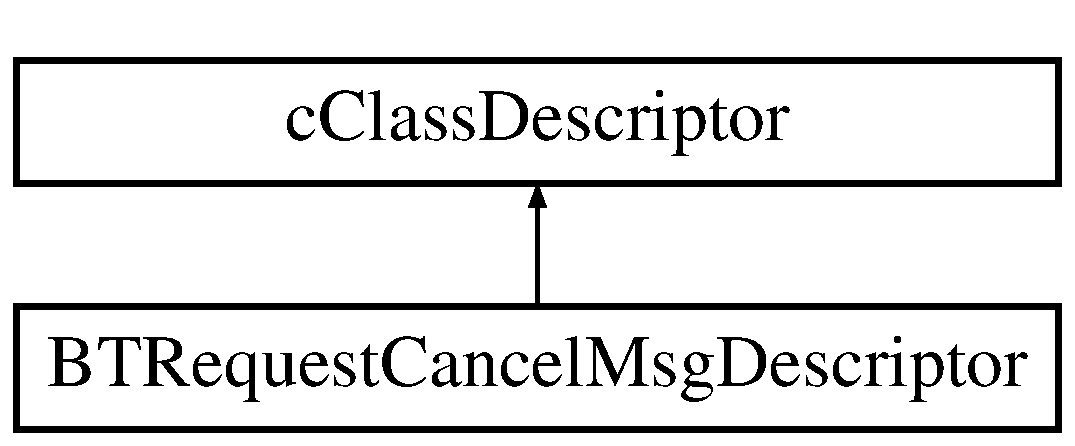
\includegraphics[height=2.000000cm]{classBTRequestCancelMsgDescriptor}
\end{center}
\end{figure}
\subsection*{Public Member Functions}
\begin{DoxyCompactItemize}
\item 
\hyperlink{classBTRequestCancelMsgDescriptor_a7121a1529ca6e29776cd6727889a177f}{B\+T\+Request\+Cancel\+Msg\+Descriptor} ()
\item 
virtual \hyperlink{classBTRequestCancelMsgDescriptor_a443e8739e46cd86bcb238c6f0d3b6256}{$\sim$\+B\+T\+Request\+Cancel\+Msg\+Descriptor} ()
\item 
virtual bool \hyperlink{classBTRequestCancelMsgDescriptor_a8ce8da495d3baf79d445061a9f88f4b9}{does\+Support} (c\+Object $\ast$obj) const 
\item 
virtual const char $\ast$ \hyperlink{classBTRequestCancelMsgDescriptor_a6fd345e4449fc27cc056c8ab009db4cf}{get\+Property} (const char $\ast$propertyname) const 
\item 
virtual int \hyperlink{classBTRequestCancelMsgDescriptor_af1ef3838ebf23aa5915624d0d48d3041}{get\+Field\+Count} (void $\ast$object) const 
\item 
virtual const char $\ast$ \hyperlink{classBTRequestCancelMsgDescriptor_a840113113837534733d2671b0ffe44d2}{get\+Field\+Name} (void $\ast$object, int field) const 
\item 
virtual int \hyperlink{classBTRequestCancelMsgDescriptor_a90c03404cd1373dd0782c2eed2dc89c8}{find\+Field} (void $\ast$object, const char $\ast$field\+Name) const 
\item 
virtual unsigned int \hyperlink{classBTRequestCancelMsgDescriptor_a87c421426ac968920409bd79693c1fdd}{get\+Field\+Type\+Flags} (void $\ast$object, int field) const 
\item 
virtual const char $\ast$ \hyperlink{classBTRequestCancelMsgDescriptor_afe0ecf5784029929a18ee58a4da78c67}{get\+Field\+Type\+String} (void $\ast$object, int field) const 
\item 
virtual const char $\ast$ \hyperlink{classBTRequestCancelMsgDescriptor_a621b6ebc8169c9ad9a3cc53d783152d5}{get\+Field\+Property} (void $\ast$object, int field, const char $\ast$propertyname) const 
\item 
virtual int \hyperlink{classBTRequestCancelMsgDescriptor_a2adab05184edbec1935786a73bec3fa6}{get\+Array\+Size} (void $\ast$object, int field) const 
\item 
virtual std\+::string \hyperlink{classBTRequestCancelMsgDescriptor_a37a35440136025afb9ef3c5ef8b0617d}{get\+Field\+As\+String} (void $\ast$object, int field, int i) const 
\item 
virtual bool \hyperlink{classBTRequestCancelMsgDescriptor_a1e7053ac242faf993d95d4438b933456}{set\+Field\+As\+String} (void $\ast$object, int field, int i, const char $\ast$value) const 
\item 
virtual const char $\ast$ \hyperlink{classBTRequestCancelMsgDescriptor_a866b5c0e67e036f83e100b6c48cb8ae0}{get\+Field\+Struct\+Name} (void $\ast$object, int field) const 
\item 
virtual void $\ast$ \hyperlink{classBTRequestCancelMsgDescriptor_a4c0e36f4f586f4dbc004a80e82925fe2}{get\+Field\+Struct\+Pointer} (void $\ast$object, int field, int i) const 
\end{DoxyCompactItemize}


\subsection{Constructor \& Destructor Documentation}
\hypertarget{classBTRequestCancelMsgDescriptor_a7121a1529ca6e29776cd6727889a177f}{}\index{B\+T\+Request\+Cancel\+Msg\+Descriptor@{B\+T\+Request\+Cancel\+Msg\+Descriptor}!B\+T\+Request\+Cancel\+Msg\+Descriptor@{B\+T\+Request\+Cancel\+Msg\+Descriptor}}
\index{B\+T\+Request\+Cancel\+Msg\+Descriptor@{B\+T\+Request\+Cancel\+Msg\+Descriptor}!B\+T\+Request\+Cancel\+Msg\+Descriptor@{B\+T\+Request\+Cancel\+Msg\+Descriptor}}
\subsubsection[{B\+T\+Request\+Cancel\+Msg\+Descriptor()}]{\setlength{\rightskip}{0pt plus 5cm}B\+T\+Request\+Cancel\+Msg\+Descriptor\+::\+B\+T\+Request\+Cancel\+Msg\+Descriptor (
\begin{DoxyParamCaption}
{}
\end{DoxyParamCaption}
)}\label{classBTRequestCancelMsgDescriptor_a7121a1529ca6e29776cd6727889a177f}
\hypertarget{classBTRequestCancelMsgDescriptor_a443e8739e46cd86bcb238c6f0d3b6256}{}\index{B\+T\+Request\+Cancel\+Msg\+Descriptor@{B\+T\+Request\+Cancel\+Msg\+Descriptor}!````~B\+T\+Request\+Cancel\+Msg\+Descriptor@{$\sim$\+B\+T\+Request\+Cancel\+Msg\+Descriptor}}
\index{````~B\+T\+Request\+Cancel\+Msg\+Descriptor@{$\sim$\+B\+T\+Request\+Cancel\+Msg\+Descriptor}!B\+T\+Request\+Cancel\+Msg\+Descriptor@{B\+T\+Request\+Cancel\+Msg\+Descriptor}}
\subsubsection[{$\sim$\+B\+T\+Request\+Cancel\+Msg\+Descriptor()}]{\setlength{\rightskip}{0pt plus 5cm}B\+T\+Request\+Cancel\+Msg\+Descriptor\+::$\sim$\+B\+T\+Request\+Cancel\+Msg\+Descriptor (
\begin{DoxyParamCaption}
{}
\end{DoxyParamCaption}
)\hspace{0.3cm}{\ttfamily [virtual]}}\label{classBTRequestCancelMsgDescriptor_a443e8739e46cd86bcb238c6f0d3b6256}


\subsection{Member Function Documentation}
\hypertarget{classBTRequestCancelMsgDescriptor_a8ce8da495d3baf79d445061a9f88f4b9}{}\index{B\+T\+Request\+Cancel\+Msg\+Descriptor@{B\+T\+Request\+Cancel\+Msg\+Descriptor}!does\+Support@{does\+Support}}
\index{does\+Support@{does\+Support}!B\+T\+Request\+Cancel\+Msg\+Descriptor@{B\+T\+Request\+Cancel\+Msg\+Descriptor}}
\subsubsection[{does\+Support(c\+Object $\ast$obj) const }]{\setlength{\rightskip}{0pt plus 5cm}bool B\+T\+Request\+Cancel\+Msg\+Descriptor\+::does\+Support (
\begin{DoxyParamCaption}
\item[{c\+Object $\ast$}]{obj}
\end{DoxyParamCaption}
) const\hspace{0.3cm}{\ttfamily [virtual]}}\label{classBTRequestCancelMsgDescriptor_a8ce8da495d3baf79d445061a9f88f4b9}
\hypertarget{classBTRequestCancelMsgDescriptor_a90c03404cd1373dd0782c2eed2dc89c8}{}\index{B\+T\+Request\+Cancel\+Msg\+Descriptor@{B\+T\+Request\+Cancel\+Msg\+Descriptor}!find\+Field@{find\+Field}}
\index{find\+Field@{find\+Field}!B\+T\+Request\+Cancel\+Msg\+Descriptor@{B\+T\+Request\+Cancel\+Msg\+Descriptor}}
\subsubsection[{find\+Field(void $\ast$object, const char $\ast$field\+Name) const }]{\setlength{\rightskip}{0pt plus 5cm}int B\+T\+Request\+Cancel\+Msg\+Descriptor\+::find\+Field (
\begin{DoxyParamCaption}
\item[{void $\ast$}]{object, }
\item[{const char $\ast$}]{field\+Name}
\end{DoxyParamCaption}
) const\hspace{0.3cm}{\ttfamily [virtual]}}\label{classBTRequestCancelMsgDescriptor_a90c03404cd1373dd0782c2eed2dc89c8}
\hypertarget{classBTRequestCancelMsgDescriptor_a2adab05184edbec1935786a73bec3fa6}{}\index{B\+T\+Request\+Cancel\+Msg\+Descriptor@{B\+T\+Request\+Cancel\+Msg\+Descriptor}!get\+Array\+Size@{get\+Array\+Size}}
\index{get\+Array\+Size@{get\+Array\+Size}!B\+T\+Request\+Cancel\+Msg\+Descriptor@{B\+T\+Request\+Cancel\+Msg\+Descriptor}}
\subsubsection[{get\+Array\+Size(void $\ast$object, int field) const }]{\setlength{\rightskip}{0pt plus 5cm}int B\+T\+Request\+Cancel\+Msg\+Descriptor\+::get\+Array\+Size (
\begin{DoxyParamCaption}
\item[{void $\ast$}]{object, }
\item[{int}]{field}
\end{DoxyParamCaption}
) const\hspace{0.3cm}{\ttfamily [virtual]}}\label{classBTRequestCancelMsgDescriptor_a2adab05184edbec1935786a73bec3fa6}
\hypertarget{classBTRequestCancelMsgDescriptor_a37a35440136025afb9ef3c5ef8b0617d}{}\index{B\+T\+Request\+Cancel\+Msg\+Descriptor@{B\+T\+Request\+Cancel\+Msg\+Descriptor}!get\+Field\+As\+String@{get\+Field\+As\+String}}
\index{get\+Field\+As\+String@{get\+Field\+As\+String}!B\+T\+Request\+Cancel\+Msg\+Descriptor@{B\+T\+Request\+Cancel\+Msg\+Descriptor}}
\subsubsection[{get\+Field\+As\+String(void $\ast$object, int field, int i) const }]{\setlength{\rightskip}{0pt plus 5cm}std\+::string B\+T\+Request\+Cancel\+Msg\+Descriptor\+::get\+Field\+As\+String (
\begin{DoxyParamCaption}
\item[{void $\ast$}]{object, }
\item[{int}]{field, }
\item[{int}]{i}
\end{DoxyParamCaption}
) const\hspace{0.3cm}{\ttfamily [virtual]}}\label{classBTRequestCancelMsgDescriptor_a37a35440136025afb9ef3c5ef8b0617d}
\hypertarget{classBTRequestCancelMsgDescriptor_af1ef3838ebf23aa5915624d0d48d3041}{}\index{B\+T\+Request\+Cancel\+Msg\+Descriptor@{B\+T\+Request\+Cancel\+Msg\+Descriptor}!get\+Field\+Count@{get\+Field\+Count}}
\index{get\+Field\+Count@{get\+Field\+Count}!B\+T\+Request\+Cancel\+Msg\+Descriptor@{B\+T\+Request\+Cancel\+Msg\+Descriptor}}
\subsubsection[{get\+Field\+Count(void $\ast$object) const }]{\setlength{\rightskip}{0pt plus 5cm}int B\+T\+Request\+Cancel\+Msg\+Descriptor\+::get\+Field\+Count (
\begin{DoxyParamCaption}
\item[{void $\ast$}]{object}
\end{DoxyParamCaption}
) const\hspace{0.3cm}{\ttfamily [virtual]}}\label{classBTRequestCancelMsgDescriptor_af1ef3838ebf23aa5915624d0d48d3041}
\hypertarget{classBTRequestCancelMsgDescriptor_a840113113837534733d2671b0ffe44d2}{}\index{B\+T\+Request\+Cancel\+Msg\+Descriptor@{B\+T\+Request\+Cancel\+Msg\+Descriptor}!get\+Field\+Name@{get\+Field\+Name}}
\index{get\+Field\+Name@{get\+Field\+Name}!B\+T\+Request\+Cancel\+Msg\+Descriptor@{B\+T\+Request\+Cancel\+Msg\+Descriptor}}
\subsubsection[{get\+Field\+Name(void $\ast$object, int field) const }]{\setlength{\rightskip}{0pt plus 5cm}const char $\ast$ B\+T\+Request\+Cancel\+Msg\+Descriptor\+::get\+Field\+Name (
\begin{DoxyParamCaption}
\item[{void $\ast$}]{object, }
\item[{int}]{field}
\end{DoxyParamCaption}
) const\hspace{0.3cm}{\ttfamily [virtual]}}\label{classBTRequestCancelMsgDescriptor_a840113113837534733d2671b0ffe44d2}
\hypertarget{classBTRequestCancelMsgDescriptor_a621b6ebc8169c9ad9a3cc53d783152d5}{}\index{B\+T\+Request\+Cancel\+Msg\+Descriptor@{B\+T\+Request\+Cancel\+Msg\+Descriptor}!get\+Field\+Property@{get\+Field\+Property}}
\index{get\+Field\+Property@{get\+Field\+Property}!B\+T\+Request\+Cancel\+Msg\+Descriptor@{B\+T\+Request\+Cancel\+Msg\+Descriptor}}
\subsubsection[{get\+Field\+Property(void $\ast$object, int field, const char $\ast$propertyname) const }]{\setlength{\rightskip}{0pt plus 5cm}const char $\ast$ B\+T\+Request\+Cancel\+Msg\+Descriptor\+::get\+Field\+Property (
\begin{DoxyParamCaption}
\item[{void $\ast$}]{object, }
\item[{int}]{field, }
\item[{const char $\ast$}]{propertyname}
\end{DoxyParamCaption}
) const\hspace{0.3cm}{\ttfamily [virtual]}}\label{classBTRequestCancelMsgDescriptor_a621b6ebc8169c9ad9a3cc53d783152d5}
\hypertarget{classBTRequestCancelMsgDescriptor_a866b5c0e67e036f83e100b6c48cb8ae0}{}\index{B\+T\+Request\+Cancel\+Msg\+Descriptor@{B\+T\+Request\+Cancel\+Msg\+Descriptor}!get\+Field\+Struct\+Name@{get\+Field\+Struct\+Name}}
\index{get\+Field\+Struct\+Name@{get\+Field\+Struct\+Name}!B\+T\+Request\+Cancel\+Msg\+Descriptor@{B\+T\+Request\+Cancel\+Msg\+Descriptor}}
\subsubsection[{get\+Field\+Struct\+Name(void $\ast$object, int field) const }]{\setlength{\rightskip}{0pt plus 5cm}const char $\ast$ B\+T\+Request\+Cancel\+Msg\+Descriptor\+::get\+Field\+Struct\+Name (
\begin{DoxyParamCaption}
\item[{void $\ast$}]{object, }
\item[{int}]{field}
\end{DoxyParamCaption}
) const\hspace{0.3cm}{\ttfamily [virtual]}}\label{classBTRequestCancelMsgDescriptor_a866b5c0e67e036f83e100b6c48cb8ae0}
\hypertarget{classBTRequestCancelMsgDescriptor_a4c0e36f4f586f4dbc004a80e82925fe2}{}\index{B\+T\+Request\+Cancel\+Msg\+Descriptor@{B\+T\+Request\+Cancel\+Msg\+Descriptor}!get\+Field\+Struct\+Pointer@{get\+Field\+Struct\+Pointer}}
\index{get\+Field\+Struct\+Pointer@{get\+Field\+Struct\+Pointer}!B\+T\+Request\+Cancel\+Msg\+Descriptor@{B\+T\+Request\+Cancel\+Msg\+Descriptor}}
\subsubsection[{get\+Field\+Struct\+Pointer(void $\ast$object, int field, int i) const }]{\setlength{\rightskip}{0pt plus 5cm}void $\ast$ B\+T\+Request\+Cancel\+Msg\+Descriptor\+::get\+Field\+Struct\+Pointer (
\begin{DoxyParamCaption}
\item[{void $\ast$}]{object, }
\item[{int}]{field, }
\item[{int}]{i}
\end{DoxyParamCaption}
) const\hspace{0.3cm}{\ttfamily [virtual]}}\label{classBTRequestCancelMsgDescriptor_a4c0e36f4f586f4dbc004a80e82925fe2}
\hypertarget{classBTRequestCancelMsgDescriptor_a87c421426ac968920409bd79693c1fdd}{}\index{B\+T\+Request\+Cancel\+Msg\+Descriptor@{B\+T\+Request\+Cancel\+Msg\+Descriptor}!get\+Field\+Type\+Flags@{get\+Field\+Type\+Flags}}
\index{get\+Field\+Type\+Flags@{get\+Field\+Type\+Flags}!B\+T\+Request\+Cancel\+Msg\+Descriptor@{B\+T\+Request\+Cancel\+Msg\+Descriptor}}
\subsubsection[{get\+Field\+Type\+Flags(void $\ast$object, int field) const }]{\setlength{\rightskip}{0pt plus 5cm}unsigned int B\+T\+Request\+Cancel\+Msg\+Descriptor\+::get\+Field\+Type\+Flags (
\begin{DoxyParamCaption}
\item[{void $\ast$}]{object, }
\item[{int}]{field}
\end{DoxyParamCaption}
) const\hspace{0.3cm}{\ttfamily [virtual]}}\label{classBTRequestCancelMsgDescriptor_a87c421426ac968920409bd79693c1fdd}
\hypertarget{classBTRequestCancelMsgDescriptor_afe0ecf5784029929a18ee58a4da78c67}{}\index{B\+T\+Request\+Cancel\+Msg\+Descriptor@{B\+T\+Request\+Cancel\+Msg\+Descriptor}!get\+Field\+Type\+String@{get\+Field\+Type\+String}}
\index{get\+Field\+Type\+String@{get\+Field\+Type\+String}!B\+T\+Request\+Cancel\+Msg\+Descriptor@{B\+T\+Request\+Cancel\+Msg\+Descriptor}}
\subsubsection[{get\+Field\+Type\+String(void $\ast$object, int field) const }]{\setlength{\rightskip}{0pt plus 5cm}const char $\ast$ B\+T\+Request\+Cancel\+Msg\+Descriptor\+::get\+Field\+Type\+String (
\begin{DoxyParamCaption}
\item[{void $\ast$}]{object, }
\item[{int}]{field}
\end{DoxyParamCaption}
) const\hspace{0.3cm}{\ttfamily [virtual]}}\label{classBTRequestCancelMsgDescriptor_afe0ecf5784029929a18ee58a4da78c67}
\hypertarget{classBTRequestCancelMsgDescriptor_a6fd345e4449fc27cc056c8ab009db4cf}{}\index{B\+T\+Request\+Cancel\+Msg\+Descriptor@{B\+T\+Request\+Cancel\+Msg\+Descriptor}!get\+Property@{get\+Property}}
\index{get\+Property@{get\+Property}!B\+T\+Request\+Cancel\+Msg\+Descriptor@{B\+T\+Request\+Cancel\+Msg\+Descriptor}}
\subsubsection[{get\+Property(const char $\ast$propertyname) const }]{\setlength{\rightskip}{0pt plus 5cm}const char $\ast$ B\+T\+Request\+Cancel\+Msg\+Descriptor\+::get\+Property (
\begin{DoxyParamCaption}
\item[{const char $\ast$}]{propertyname}
\end{DoxyParamCaption}
) const\hspace{0.3cm}{\ttfamily [virtual]}}\label{classBTRequestCancelMsgDescriptor_a6fd345e4449fc27cc056c8ab009db4cf}
\hypertarget{classBTRequestCancelMsgDescriptor_a1e7053ac242faf993d95d4438b933456}{}\index{B\+T\+Request\+Cancel\+Msg\+Descriptor@{B\+T\+Request\+Cancel\+Msg\+Descriptor}!set\+Field\+As\+String@{set\+Field\+As\+String}}
\index{set\+Field\+As\+String@{set\+Field\+As\+String}!B\+T\+Request\+Cancel\+Msg\+Descriptor@{B\+T\+Request\+Cancel\+Msg\+Descriptor}}
\subsubsection[{set\+Field\+As\+String(void $\ast$object, int field, int i, const char $\ast$value) const }]{\setlength{\rightskip}{0pt plus 5cm}bool B\+T\+Request\+Cancel\+Msg\+Descriptor\+::set\+Field\+As\+String (
\begin{DoxyParamCaption}
\item[{void $\ast$}]{object, }
\item[{int}]{field, }
\item[{int}]{i, }
\item[{const char $\ast$}]{value}
\end{DoxyParamCaption}
) const\hspace{0.3cm}{\ttfamily [virtual]}}\label{classBTRequestCancelMsgDescriptor_a1e7053ac242faf993d95d4438b933456}


The documentation for this class was generated from the following file\+:\begin{DoxyCompactItemize}
\item 
\hyperlink{BTPeerWireMsg__m_8cc}{B\+T\+Peer\+Wire\+Msg\+\_\+m.\+cc}\end{DoxyCompactItemize}

\hypertarget{classBTStatistics}{}\section{B\+T\+Statistics Class Reference}
\label{classBTStatistics}\index{B\+T\+Statistics@{B\+T\+Statistics}}


{\ttfamily \#include $<$B\+T\+Statistics.\+h$>$}

Inheritance diagram for B\+T\+Statistics\+:\begin{figure}[H]
\begin{center}
\leavevmode
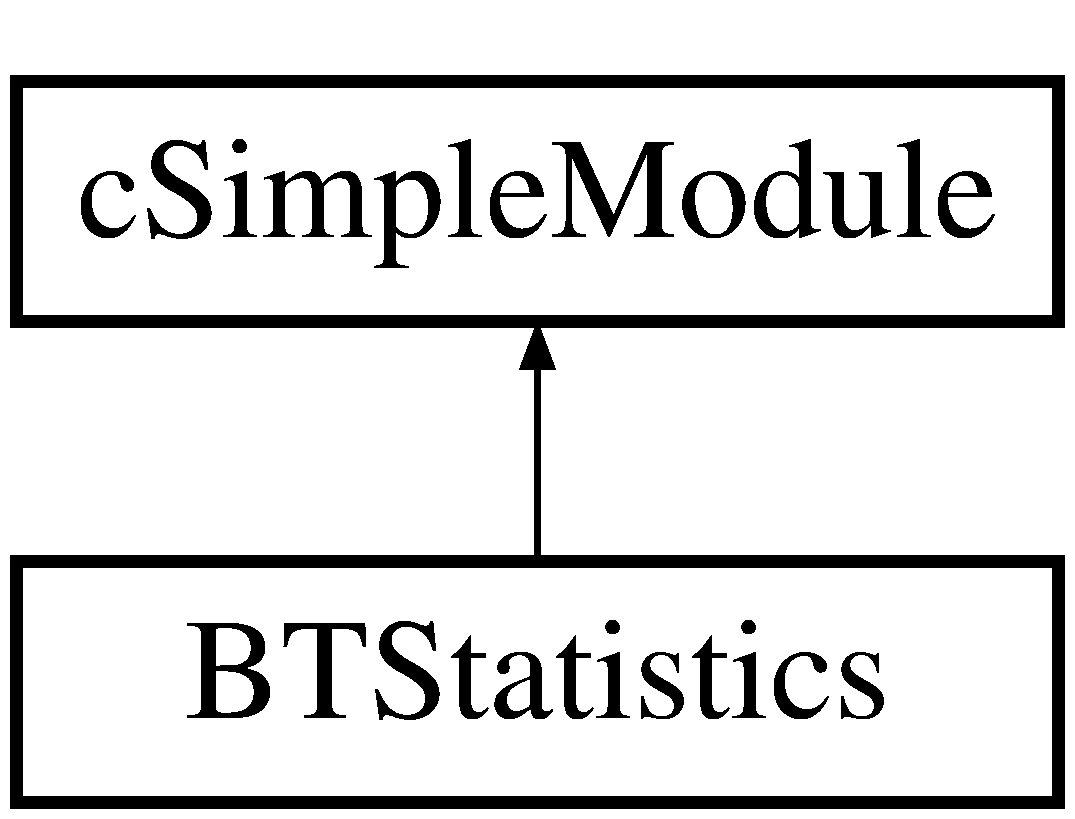
\includegraphics[height=2.000000cm]{classBTStatistics}
\end{center}
\end{figure}
\subsection*{Public Member Functions}
\begin{DoxyCompactItemize}
\item 
\hyperlink{classBTStatistics_ac45d4907a45437ff46e22673663e3039}{$\sim$\+B\+T\+Statistics} ()
\end{DoxyCompactItemize}
\subsection*{Protected Member Functions}
\begin{DoxyCompactItemize}
\item 
void \hyperlink{classBTStatistics_a019a72be755d8da5fe55096fc9859780}{check\+Finish} ()
\item 
virtual void \hyperlink{classBTStatistics_ade8599c76eddd32a9de2b147ad206a5c}{initialize} ()
\item 
virtual void \hyperlink{classBTStatistics_aa8d25bd062c2338cae68e798496c8f41}{handle\+Message} (c\+Message $\ast$msg)
\item 
virtual void \hyperlink{classBTStatistics_a79818ddd3f1e516bbf5dc34c7ff2aee4}{finish} ()
\item 
void \hyperlink{classBTStatistics_a7c2bd895d14a2b266847284e21293422}{do\+Finish} ()
\end{DoxyCompactItemize}
\subsection*{Protected Attributes}
\begin{DoxyCompactItemize}
\item 
int \hyperlink{classBTStatistics_aa9663e0a709e2bbe2b4859acc0c2b72b}{current\+Terminal\+Num}
\item 
int \hyperlink{classBTStatistics_a85c632cdb7b255da257b65e5370000b4}{target\+Overlay\+Terminal\+Num}
\item 
c\+Std\+Dev $\ast$ \hyperlink{classBTStatistics_a1342bc01b82315391b10d5c0560b4ee2}{dw\+Success}
\item 
c\+Out\+Vector \hyperlink{classBTStatistics_a3bf710ae5862b7c6b171a70ed570dec4}{dw\+Success\+\_\+vec}
\item 
c\+Std\+Dev $\ast$ \hyperlink{classBTStatistics_ad6701a3f8b96df4e7535020f9f57c8e6}{num\+Block\+Fail}
\item 
c\+Out\+Vector \hyperlink{classBTStatistics_ab9542f9a68503485c303d5d6667c8a44}{num\+Block\+Fail\+\_\+vec}
\item 
c\+Std\+Dev $\ast$ \hyperlink{classBTStatistics_a7ea82ebc767d80852b4d4857cc86c614}{data\+Providers}
\item 
c\+Out\+Vector \hyperlink{classBTStatistics_aa97b13fd73e1120a01c050fdc05e1eb0}{data\+Providers\+\_\+vec}
\item 
c\+Std\+Dev $\ast$ \hyperlink{classBTStatistics_ab0754ded61dc5b410ba3345415eb0cbe}{num\+Seeder\+Blocks}
\item 
c\+Out\+Vector \hyperlink{classBTStatistics_a6ff3cdec7cc91846c2482ebf1a1ebfe6}{num\+Seeder\+Blocks\+\_\+vec}
\item 
c\+Std\+Dev $\ast$ \hyperlink{classBTStatistics_ac24ef388a8ae35c9e4427dc146db48be}{num\+Hits}
\item 
c\+Out\+Vector \hyperlink{classBTStatistics_af717deda266c06bcbb0395b4e4d70908}{num\+Hits\+\_\+vec}
\item 
c\+Std\+Dev $\ast$ \hyperlink{classBTStatistics_aa1fc0cbf7c6596091752c923da48b334}{num\+Misses}
\item 
c\+Out\+Vector \hyperlink{classBTStatistics_aa2be128331e707564905616f8be6e113}{num\+Misses\+\_\+vec}
\end{DoxyCompactItemize}


\subsection{Detailed Description}
Module that calculates the multicast groups sizes and randomly selects their participants (receivers and sender). It is also used for global statistics measurement such as stretch.

\begin{DoxyAuthor}{Author}
Konstantinos Katsaros 
\end{DoxyAuthor}


\subsection{Constructor \& Destructor Documentation}
\hypertarget{classBTStatistics_ac45d4907a45437ff46e22673663e3039}{}\index{B\+T\+Statistics@{B\+T\+Statistics}!````~B\+T\+Statistics@{$\sim$\+B\+T\+Statistics}}
\index{````~B\+T\+Statistics@{$\sim$\+B\+T\+Statistics}!B\+T\+Statistics@{B\+T\+Statistics}}
\subsubsection[{$\sim$\+B\+T\+Statistics()}]{\setlength{\rightskip}{0pt plus 5cm}B\+T\+Statistics\+::$\sim$\+B\+T\+Statistics (
\begin{DoxyParamCaption}
{}
\end{DoxyParamCaption}
)}\label{classBTStatistics_ac45d4907a45437ff46e22673663e3039}
Destructor 

\subsection{Member Function Documentation}
\hypertarget{classBTStatistics_a019a72be755d8da5fe55096fc9859780}{}\index{B\+T\+Statistics@{B\+T\+Statistics}!check\+Finish@{check\+Finish}}
\index{check\+Finish@{check\+Finish}!B\+T\+Statistics@{B\+T\+Statistics}}
\subsubsection[{check\+Finish()}]{\setlength{\rightskip}{0pt plus 5cm}void B\+T\+Statistics\+::check\+Finish (
\begin{DoxyParamCaption}
{}
\end{DoxyParamCaption}
)\hspace{0.3cm}{\ttfamily [protected]}}\label{classBTStatistics_a019a72be755d8da5fe55096fc9859780}
Check whether the statistics collection has completed \hypertarget{classBTStatistics_a7c2bd895d14a2b266847284e21293422}{}\index{B\+T\+Statistics@{B\+T\+Statistics}!do\+Finish@{do\+Finish}}
\index{do\+Finish@{do\+Finish}!B\+T\+Statistics@{B\+T\+Statistics}}
\subsubsection[{do\+Finish()}]{\setlength{\rightskip}{0pt plus 5cm}void B\+T\+Statistics\+::do\+Finish (
\begin{DoxyParamCaption}
{}
\end{DoxyParamCaption}
)\hspace{0.3cm}{\ttfamily [protected]}}\label{classBTStatistics_a7c2bd895d14a2b266847284e21293422}
Do the actual \hyperlink{classBTStatistics_a79818ddd3f1e516bbf5dc34c7ff2aee4}{finish()} call and record scalars \hypertarget{classBTStatistics_a79818ddd3f1e516bbf5dc34c7ff2aee4}{}\index{B\+T\+Statistics@{B\+T\+Statistics}!finish@{finish}}
\index{finish@{finish}!B\+T\+Statistics@{B\+T\+Statistics}}
\subsubsection[{finish()}]{\setlength{\rightskip}{0pt plus 5cm}void B\+T\+Statistics\+::finish (
\begin{DoxyParamCaption}
{}
\end{DoxyParamCaption}
)\hspace{0.3cm}{\ttfamily [protected]}, {\ttfamily [virtual]}}\label{classBTStatistics_a79818ddd3f1e516bbf5dc34c7ff2aee4}
Finish member function of module \hypertarget{classBTStatistics_aa8d25bd062c2338cae68e798496c8f41}{}\index{B\+T\+Statistics@{B\+T\+Statistics}!handle\+Message@{handle\+Message}}
\index{handle\+Message@{handle\+Message}!B\+T\+Statistics@{B\+T\+Statistics}}
\subsubsection[{handle\+Message(c\+Message $\ast$msg)}]{\setlength{\rightskip}{0pt plus 5cm}void B\+T\+Statistics\+::handle\+Message (
\begin{DoxyParamCaption}
\item[{c\+Message $\ast$}]{msg}
\end{DoxyParamCaption}
)\hspace{0.3cm}{\ttfamily [protected]}, {\ttfamily [virtual]}}\label{classBTStatistics_aa8d25bd062c2338cae68e798496c8f41}
Handle\+Message member function of module \hypertarget{classBTStatistics_ade8599c76eddd32a9de2b147ad206a5c}{}\index{B\+T\+Statistics@{B\+T\+Statistics}!initialize@{initialize}}
\index{initialize@{initialize}!B\+T\+Statistics@{B\+T\+Statistics}}
\subsubsection[{initialize()}]{\setlength{\rightskip}{0pt plus 5cm}void B\+T\+Statistics\+::initialize (
\begin{DoxyParamCaption}
{}
\end{DoxyParamCaption}
)\hspace{0.3cm}{\ttfamily [protected]}, {\ttfamily [virtual]}}\label{classBTStatistics_ade8599c76eddd32a9de2b147ad206a5c}
Init member function of module 

\subsection{Member Data Documentation}
\hypertarget{classBTStatistics_aa9663e0a709e2bbe2b4859acc0c2b72b}{}\index{B\+T\+Statistics@{B\+T\+Statistics}!current\+Terminal\+Num@{current\+Terminal\+Num}}
\index{current\+Terminal\+Num@{current\+Terminal\+Num}!B\+T\+Statistics@{B\+T\+Statistics}}
\subsubsection[{current\+Terminal\+Num}]{\setlength{\rightskip}{0pt plus 5cm}int B\+T\+Statistics\+::current\+Terminal\+Num\hspace{0.3cm}{\ttfamily [protected]}}\label{classBTStatistics_aa9663e0a709e2bbe2b4859acc0c2b72b}
\hypertarget{classBTStatistics_a7ea82ebc767d80852b4d4857cc86c614}{}\index{B\+T\+Statistics@{B\+T\+Statistics}!data\+Providers@{data\+Providers}}
\index{data\+Providers@{data\+Providers}!B\+T\+Statistics@{B\+T\+Statistics}}
\subsubsection[{data\+Providers}]{\setlength{\rightskip}{0pt plus 5cm}c\+Std\+Dev$\ast$ B\+T\+Statistics\+::data\+Providers\hspace{0.3cm}{\ttfamily [protected]}}\label{classBTStatistics_a7ea82ebc767d80852b4d4857cc86c614}
\hypertarget{classBTStatistics_aa97b13fd73e1120a01c050fdc05e1eb0}{}\index{B\+T\+Statistics@{B\+T\+Statistics}!data\+Providers\+\_\+vec@{data\+Providers\+\_\+vec}}
\index{data\+Providers\+\_\+vec@{data\+Providers\+\_\+vec}!B\+T\+Statistics@{B\+T\+Statistics}}
\subsubsection[{data\+Providers\+\_\+vec}]{\setlength{\rightskip}{0pt plus 5cm}c\+Out\+Vector B\+T\+Statistics\+::data\+Providers\+\_\+vec\hspace{0.3cm}{\ttfamily [protected]}}\label{classBTStatistics_aa97b13fd73e1120a01c050fdc05e1eb0}
\hypertarget{classBTStatistics_a1342bc01b82315391b10d5c0560b4ee2}{}\index{B\+T\+Statistics@{B\+T\+Statistics}!dw\+Success@{dw\+Success}}
\index{dw\+Success@{dw\+Success}!B\+T\+Statistics@{B\+T\+Statistics}}
\subsubsection[{dw\+Success}]{\setlength{\rightskip}{0pt plus 5cm}c\+Std\+Dev$\ast$ B\+T\+Statistics\+::dw\+Success\hspace{0.3cm}{\ttfamily [protected]}}\label{classBTStatistics_a1342bc01b82315391b10d5c0560b4ee2}
\hypertarget{classBTStatistics_a3bf710ae5862b7c6b171a70ed570dec4}{}\index{B\+T\+Statistics@{B\+T\+Statistics}!dw\+Success\+\_\+vec@{dw\+Success\+\_\+vec}}
\index{dw\+Success\+\_\+vec@{dw\+Success\+\_\+vec}!B\+T\+Statistics@{B\+T\+Statistics}}
\subsubsection[{dw\+Success\+\_\+vec}]{\setlength{\rightskip}{0pt plus 5cm}c\+Out\+Vector B\+T\+Statistics\+::dw\+Success\+\_\+vec\hspace{0.3cm}{\ttfamily [protected]}}\label{classBTStatistics_a3bf710ae5862b7c6b171a70ed570dec4}
\hypertarget{classBTStatistics_ad6701a3f8b96df4e7535020f9f57c8e6}{}\index{B\+T\+Statistics@{B\+T\+Statistics}!num\+Block\+Fail@{num\+Block\+Fail}}
\index{num\+Block\+Fail@{num\+Block\+Fail}!B\+T\+Statistics@{B\+T\+Statistics}}
\subsubsection[{num\+Block\+Fail}]{\setlength{\rightskip}{0pt plus 5cm}c\+Std\+Dev$\ast$ B\+T\+Statistics\+::num\+Block\+Fail\hspace{0.3cm}{\ttfamily [protected]}}\label{classBTStatistics_ad6701a3f8b96df4e7535020f9f57c8e6}
\hypertarget{classBTStatistics_ab9542f9a68503485c303d5d6667c8a44}{}\index{B\+T\+Statistics@{B\+T\+Statistics}!num\+Block\+Fail\+\_\+vec@{num\+Block\+Fail\+\_\+vec}}
\index{num\+Block\+Fail\+\_\+vec@{num\+Block\+Fail\+\_\+vec}!B\+T\+Statistics@{B\+T\+Statistics}}
\subsubsection[{num\+Block\+Fail\+\_\+vec}]{\setlength{\rightskip}{0pt plus 5cm}c\+Out\+Vector B\+T\+Statistics\+::num\+Block\+Fail\+\_\+vec\hspace{0.3cm}{\ttfamily [protected]}}\label{classBTStatistics_ab9542f9a68503485c303d5d6667c8a44}
\hypertarget{classBTStatistics_ac24ef388a8ae35c9e4427dc146db48be}{}\index{B\+T\+Statistics@{B\+T\+Statistics}!num\+Hits@{num\+Hits}}
\index{num\+Hits@{num\+Hits}!B\+T\+Statistics@{B\+T\+Statistics}}
\subsubsection[{num\+Hits}]{\setlength{\rightskip}{0pt plus 5cm}c\+Std\+Dev$\ast$ B\+T\+Statistics\+::num\+Hits\hspace{0.3cm}{\ttfamily [protected]}}\label{classBTStatistics_ac24ef388a8ae35c9e4427dc146db48be}
\hypertarget{classBTStatistics_af717deda266c06bcbb0395b4e4d70908}{}\index{B\+T\+Statistics@{B\+T\+Statistics}!num\+Hits\+\_\+vec@{num\+Hits\+\_\+vec}}
\index{num\+Hits\+\_\+vec@{num\+Hits\+\_\+vec}!B\+T\+Statistics@{B\+T\+Statistics}}
\subsubsection[{num\+Hits\+\_\+vec}]{\setlength{\rightskip}{0pt plus 5cm}c\+Out\+Vector B\+T\+Statistics\+::num\+Hits\+\_\+vec\hspace{0.3cm}{\ttfamily [protected]}}\label{classBTStatistics_af717deda266c06bcbb0395b4e4d70908}
\hypertarget{classBTStatistics_aa1fc0cbf7c6596091752c923da48b334}{}\index{B\+T\+Statistics@{B\+T\+Statistics}!num\+Misses@{num\+Misses}}
\index{num\+Misses@{num\+Misses}!B\+T\+Statistics@{B\+T\+Statistics}}
\subsubsection[{num\+Misses}]{\setlength{\rightskip}{0pt plus 5cm}c\+Std\+Dev$\ast$ B\+T\+Statistics\+::num\+Misses\hspace{0.3cm}{\ttfamily [protected]}}\label{classBTStatistics_aa1fc0cbf7c6596091752c923da48b334}
\hypertarget{classBTStatistics_aa2be128331e707564905616f8be6e113}{}\index{B\+T\+Statistics@{B\+T\+Statistics}!num\+Misses\+\_\+vec@{num\+Misses\+\_\+vec}}
\index{num\+Misses\+\_\+vec@{num\+Misses\+\_\+vec}!B\+T\+Statistics@{B\+T\+Statistics}}
\subsubsection[{num\+Misses\+\_\+vec}]{\setlength{\rightskip}{0pt plus 5cm}c\+Out\+Vector B\+T\+Statistics\+::num\+Misses\+\_\+vec\hspace{0.3cm}{\ttfamily [protected]}}\label{classBTStatistics_aa2be128331e707564905616f8be6e113}
\hypertarget{classBTStatistics_ab0754ded61dc5b410ba3345415eb0cbe}{}\index{B\+T\+Statistics@{B\+T\+Statistics}!num\+Seeder\+Blocks@{num\+Seeder\+Blocks}}
\index{num\+Seeder\+Blocks@{num\+Seeder\+Blocks}!B\+T\+Statistics@{B\+T\+Statistics}}
\subsubsection[{num\+Seeder\+Blocks}]{\setlength{\rightskip}{0pt plus 5cm}c\+Std\+Dev$\ast$ B\+T\+Statistics\+::num\+Seeder\+Blocks\hspace{0.3cm}{\ttfamily [protected]}}\label{classBTStatistics_ab0754ded61dc5b410ba3345415eb0cbe}
\hypertarget{classBTStatistics_a6ff3cdec7cc91846c2482ebf1a1ebfe6}{}\index{B\+T\+Statistics@{B\+T\+Statistics}!num\+Seeder\+Blocks\+\_\+vec@{num\+Seeder\+Blocks\+\_\+vec}}
\index{num\+Seeder\+Blocks\+\_\+vec@{num\+Seeder\+Blocks\+\_\+vec}!B\+T\+Statistics@{B\+T\+Statistics}}
\subsubsection[{num\+Seeder\+Blocks\+\_\+vec}]{\setlength{\rightskip}{0pt plus 5cm}c\+Out\+Vector B\+T\+Statistics\+::num\+Seeder\+Blocks\+\_\+vec\hspace{0.3cm}{\ttfamily [protected]}}\label{classBTStatistics_a6ff3cdec7cc91846c2482ebf1a1ebfe6}
\hypertarget{classBTStatistics_a85c632cdb7b255da257b65e5370000b4}{}\index{B\+T\+Statistics@{B\+T\+Statistics}!target\+Overlay\+Terminal\+Num@{target\+Overlay\+Terminal\+Num}}
\index{target\+Overlay\+Terminal\+Num@{target\+Overlay\+Terminal\+Num}!B\+T\+Statistics@{B\+T\+Statistics}}
\subsubsection[{target\+Overlay\+Terminal\+Num}]{\setlength{\rightskip}{0pt plus 5cm}int B\+T\+Statistics\+::target\+Overlay\+Terminal\+Num\hspace{0.3cm}{\ttfamily [protected]}}\label{classBTStatistics_a85c632cdb7b255da257b65e5370000b4}


The documentation for this class was generated from the following files\+:\begin{DoxyCompactItemize}
\item 
\hyperlink{BTStatistics_8h}{B\+T\+Statistics.\+h}\item 
\hyperlink{BTStatistics_8cc}{B\+T\+Statistics.\+cc}\end{DoxyCompactItemize}

\hypertarget{classBTStatisticsDWLMsg}{}\section{B\+T\+Statistics\+D\+W\+L\+Msg Class Reference}
\label{classBTStatisticsDWLMsg}\index{B\+T\+Statistics\+D\+W\+L\+Msg@{B\+T\+Statistics\+D\+W\+L\+Msg}}


{\ttfamily \#include $<$B\+T\+Statistics\+Msg\+\_\+m.\+h$>$}

Inheritance diagram for B\+T\+Statistics\+D\+W\+L\+Msg\+:\begin{figure}[H]
\begin{center}
\leavevmode
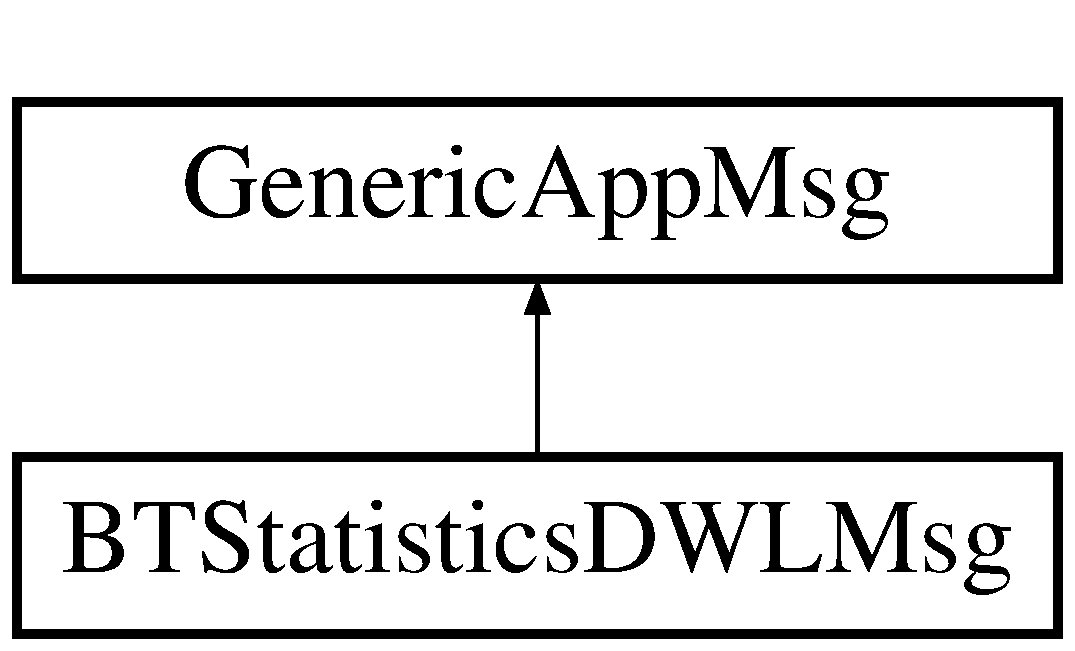
\includegraphics[height=2.000000cm]{classBTStatisticsDWLMsg}
\end{center}
\end{figure}
\subsection*{Public Member Functions}
\begin{DoxyCompactItemize}
\item 
\hyperlink{classBTStatisticsDWLMsg_aaa3666e7e5a800b20de90f2542b983ac}{B\+T\+Statistics\+D\+W\+L\+Msg} (const char $\ast$name=N\+U\+L\+L, int kind=0)
\item 
\hyperlink{classBTStatisticsDWLMsg_a1821f638c1037c06bfe6a844e903529b}{B\+T\+Statistics\+D\+W\+L\+Msg} (const \hyperlink{classBTStatisticsDWLMsg}{B\+T\+Statistics\+D\+W\+L\+Msg} \&other)
\item 
virtual \hyperlink{classBTStatisticsDWLMsg_aa6aa172862b6736d1165e7eb66373b87}{$\sim$\+B\+T\+Statistics\+D\+W\+L\+Msg} ()
\item 
\hyperlink{classBTStatisticsDWLMsg}{B\+T\+Statistics\+D\+W\+L\+Msg} \& \hyperlink{classBTStatisticsDWLMsg_a24e5ad7f6f829c8f84a8f408ddcffd36}{operator=} (const \hyperlink{classBTStatisticsDWLMsg}{B\+T\+Statistics\+D\+W\+L\+Msg} \&other)
\item 
virtual \hyperlink{classBTStatisticsDWLMsg}{B\+T\+Statistics\+D\+W\+L\+Msg} $\ast$ \hyperlink{classBTStatisticsDWLMsg_a346f1b869175fd19ea9993e5a91c53ff}{dup} () const 
\item 
virtual void \hyperlink{classBTStatisticsDWLMsg_a98c50fae916eb7a3896e6dc80c128daa}{parsim\+Pack} (c\+Comm\+Buffer $\ast$b)
\item 
virtual void \hyperlink{classBTStatisticsDWLMsg_a1c593fc8c67a786f0ddae3e39c11a72b}{parsim\+Unpack} (c\+Comm\+Buffer $\ast$b)
\item 
virtual double \hyperlink{classBTStatisticsDWLMsg_a4679c88bdf679797db3a84752849fb3e}{download\+Time} () const 
\item 
virtual void \hyperlink{classBTStatisticsDWLMsg_abf6d8570e06fab2b11e5a7486e32fb0c}{set\+Download\+Time} (double \hyperlink{classBTStatisticsDWLMsg_aac2d1b785397639eda222a1ca199c9b9}{download\+Time\+\_\+var})
\item 
virtual double \hyperlink{classBTStatisticsDWLMsg_a1945242a8136c7e5f153dc5202226572}{remaining\+Blocks} () const 
\item 
virtual void \hyperlink{classBTStatisticsDWLMsg_a5786113156e5ed923d012bd4f87d43fe}{set\+Remaining\+Blocks} (double \hyperlink{classBTStatisticsDWLMsg_a75864f08a2c20984746ee75831c0732c}{remaining\+Blocks\+\_\+var})
\end{DoxyCompactItemize}
\subsection*{Protected Member Functions}
\begin{DoxyCompactItemize}
\item 
bool \hyperlink{classBTStatisticsDWLMsg_a47274ebf65ba844b1c6c3fc34135591f}{operator==} (const \hyperlink{classBTStatisticsDWLMsg}{B\+T\+Statistics\+D\+W\+L\+Msg} \&)
\end{DoxyCompactItemize}
\subsection*{Protected Attributes}
\begin{DoxyCompactItemize}
\item 
double \hyperlink{classBTStatisticsDWLMsg_aac2d1b785397639eda222a1ca199c9b9}{download\+Time\+\_\+var}
\item 
double \hyperlink{classBTStatisticsDWLMsg_a75864f08a2c20984746ee75831c0732c}{remaining\+Blocks\+\_\+var}
\end{DoxyCompactItemize}


\subsection{Detailed Description}
Class generated from {\ttfamily applications/x\+Bit\+Torrent/\+B\+T\+Statistics\+Msg.\+msg} by opp\+\_\+msgc. 
\begin{DoxyPre}
message \hyperlink{classBTStatisticsDWLMsg}{BTStatisticsDWLMsg} extends GenericAppMsg
\{
    (true);\end{DoxyPre}



\begin{DoxyPre}    double downloadTime;        
    double remainingBlocks;\end{DoxyPre}



\begin{DoxyPre}\}
\end{DoxyPre}
 

\subsection{Constructor \& Destructor Documentation}
\hypertarget{classBTStatisticsDWLMsg_aaa3666e7e5a800b20de90f2542b983ac}{}\index{B\+T\+Statistics\+D\+W\+L\+Msg@{B\+T\+Statistics\+D\+W\+L\+Msg}!B\+T\+Statistics\+D\+W\+L\+Msg@{B\+T\+Statistics\+D\+W\+L\+Msg}}
\index{B\+T\+Statistics\+D\+W\+L\+Msg@{B\+T\+Statistics\+D\+W\+L\+Msg}!B\+T\+Statistics\+D\+W\+L\+Msg@{B\+T\+Statistics\+D\+W\+L\+Msg}}
\subsubsection[{B\+T\+Statistics\+D\+W\+L\+Msg(const char $\ast$name=\+N\+U\+L\+L, int kind=0)}]{\setlength{\rightskip}{0pt plus 5cm}B\+T\+Statistics\+D\+W\+L\+Msg\+::\+B\+T\+Statistics\+D\+W\+L\+Msg (
\begin{DoxyParamCaption}
\item[{const char $\ast$}]{name = {\ttfamily NULL}, }
\item[{int}]{kind = {\ttfamily 0}}
\end{DoxyParamCaption}
)}\label{classBTStatisticsDWLMsg_aaa3666e7e5a800b20de90f2542b983ac}
\hypertarget{classBTStatisticsDWLMsg_a1821f638c1037c06bfe6a844e903529b}{}\index{B\+T\+Statistics\+D\+W\+L\+Msg@{B\+T\+Statistics\+D\+W\+L\+Msg}!B\+T\+Statistics\+D\+W\+L\+Msg@{B\+T\+Statistics\+D\+W\+L\+Msg}}
\index{B\+T\+Statistics\+D\+W\+L\+Msg@{B\+T\+Statistics\+D\+W\+L\+Msg}!B\+T\+Statistics\+D\+W\+L\+Msg@{B\+T\+Statistics\+D\+W\+L\+Msg}}
\subsubsection[{B\+T\+Statistics\+D\+W\+L\+Msg(const B\+T\+Statistics\+D\+W\+L\+Msg \&other)}]{\setlength{\rightskip}{0pt plus 5cm}B\+T\+Statistics\+D\+W\+L\+Msg\+::\+B\+T\+Statistics\+D\+W\+L\+Msg (
\begin{DoxyParamCaption}
\item[{const {\bf B\+T\+Statistics\+D\+W\+L\+Msg} \&}]{other}
\end{DoxyParamCaption}
)}\label{classBTStatisticsDWLMsg_a1821f638c1037c06bfe6a844e903529b}
\hypertarget{classBTStatisticsDWLMsg_aa6aa172862b6736d1165e7eb66373b87}{}\index{B\+T\+Statistics\+D\+W\+L\+Msg@{B\+T\+Statistics\+D\+W\+L\+Msg}!````~B\+T\+Statistics\+D\+W\+L\+Msg@{$\sim$\+B\+T\+Statistics\+D\+W\+L\+Msg}}
\index{````~B\+T\+Statistics\+D\+W\+L\+Msg@{$\sim$\+B\+T\+Statistics\+D\+W\+L\+Msg}!B\+T\+Statistics\+D\+W\+L\+Msg@{B\+T\+Statistics\+D\+W\+L\+Msg}}
\subsubsection[{$\sim$\+B\+T\+Statistics\+D\+W\+L\+Msg()}]{\setlength{\rightskip}{0pt plus 5cm}B\+T\+Statistics\+D\+W\+L\+Msg\+::$\sim$\+B\+T\+Statistics\+D\+W\+L\+Msg (
\begin{DoxyParamCaption}
{}
\end{DoxyParamCaption}
)\hspace{0.3cm}{\ttfamily [virtual]}}\label{classBTStatisticsDWLMsg_aa6aa172862b6736d1165e7eb66373b87}


\subsection{Member Function Documentation}
\hypertarget{classBTStatisticsDWLMsg_a4679c88bdf679797db3a84752849fb3e}{}\index{B\+T\+Statistics\+D\+W\+L\+Msg@{B\+T\+Statistics\+D\+W\+L\+Msg}!download\+Time@{download\+Time}}
\index{download\+Time@{download\+Time}!B\+T\+Statistics\+D\+W\+L\+Msg@{B\+T\+Statistics\+D\+W\+L\+Msg}}
\subsubsection[{download\+Time() const }]{\setlength{\rightskip}{0pt plus 5cm}double B\+T\+Statistics\+D\+W\+L\+Msg\+::download\+Time (
\begin{DoxyParamCaption}
{}
\end{DoxyParamCaption}
) const\hspace{0.3cm}{\ttfamily [virtual]}}\label{classBTStatisticsDWLMsg_a4679c88bdf679797db3a84752849fb3e}
\hypertarget{classBTStatisticsDWLMsg_a346f1b869175fd19ea9993e5a91c53ff}{}\index{B\+T\+Statistics\+D\+W\+L\+Msg@{B\+T\+Statistics\+D\+W\+L\+Msg}!dup@{dup}}
\index{dup@{dup}!B\+T\+Statistics\+D\+W\+L\+Msg@{B\+T\+Statistics\+D\+W\+L\+Msg}}
\subsubsection[{dup() const }]{\setlength{\rightskip}{0pt plus 5cm}virtual {\bf B\+T\+Statistics\+D\+W\+L\+Msg}$\ast$ B\+T\+Statistics\+D\+W\+L\+Msg\+::dup (
\begin{DoxyParamCaption}
{}
\end{DoxyParamCaption}
) const\hspace{0.3cm}{\ttfamily [inline]}, {\ttfamily [virtual]}}\label{classBTStatisticsDWLMsg_a346f1b869175fd19ea9993e5a91c53ff}
\hypertarget{classBTStatisticsDWLMsg_a24e5ad7f6f829c8f84a8f408ddcffd36}{}\index{B\+T\+Statistics\+D\+W\+L\+Msg@{B\+T\+Statistics\+D\+W\+L\+Msg}!operator=@{operator=}}
\index{operator=@{operator=}!B\+T\+Statistics\+D\+W\+L\+Msg@{B\+T\+Statistics\+D\+W\+L\+Msg}}
\subsubsection[{operator=(const B\+T\+Statistics\+D\+W\+L\+Msg \&other)}]{\setlength{\rightskip}{0pt plus 5cm}{\bf B\+T\+Statistics\+D\+W\+L\+Msg} \& B\+T\+Statistics\+D\+W\+L\+Msg\+::operator= (
\begin{DoxyParamCaption}
\item[{const {\bf B\+T\+Statistics\+D\+W\+L\+Msg} \&}]{other}
\end{DoxyParamCaption}
)}\label{classBTStatisticsDWLMsg_a24e5ad7f6f829c8f84a8f408ddcffd36}
\hypertarget{classBTStatisticsDWLMsg_a47274ebf65ba844b1c6c3fc34135591f}{}\index{B\+T\+Statistics\+D\+W\+L\+Msg@{B\+T\+Statistics\+D\+W\+L\+Msg}!operator==@{operator==}}
\index{operator==@{operator==}!B\+T\+Statistics\+D\+W\+L\+Msg@{B\+T\+Statistics\+D\+W\+L\+Msg}}
\subsubsection[{operator==(const B\+T\+Statistics\+D\+W\+L\+Msg \&)}]{\setlength{\rightskip}{0pt plus 5cm}bool B\+T\+Statistics\+D\+W\+L\+Msg\+::operator== (
\begin{DoxyParamCaption}
\item[{const {\bf B\+T\+Statistics\+D\+W\+L\+Msg} \&}]{}
\end{DoxyParamCaption}
)\hspace{0.3cm}{\ttfamily [protected]}}\label{classBTStatisticsDWLMsg_a47274ebf65ba844b1c6c3fc34135591f}
\hypertarget{classBTStatisticsDWLMsg_a98c50fae916eb7a3896e6dc80c128daa}{}\index{B\+T\+Statistics\+D\+W\+L\+Msg@{B\+T\+Statistics\+D\+W\+L\+Msg}!parsim\+Pack@{parsim\+Pack}}
\index{parsim\+Pack@{parsim\+Pack}!B\+T\+Statistics\+D\+W\+L\+Msg@{B\+T\+Statistics\+D\+W\+L\+Msg}}
\subsubsection[{parsim\+Pack(c\+Comm\+Buffer $\ast$b)}]{\setlength{\rightskip}{0pt plus 5cm}void B\+T\+Statistics\+D\+W\+L\+Msg\+::parsim\+Pack (
\begin{DoxyParamCaption}
\item[{c\+Comm\+Buffer $\ast$}]{b}
\end{DoxyParamCaption}
)\hspace{0.3cm}{\ttfamily [virtual]}}\label{classBTStatisticsDWLMsg_a98c50fae916eb7a3896e6dc80c128daa}
\hypertarget{classBTStatisticsDWLMsg_a1c593fc8c67a786f0ddae3e39c11a72b}{}\index{B\+T\+Statistics\+D\+W\+L\+Msg@{B\+T\+Statistics\+D\+W\+L\+Msg}!parsim\+Unpack@{parsim\+Unpack}}
\index{parsim\+Unpack@{parsim\+Unpack}!B\+T\+Statistics\+D\+W\+L\+Msg@{B\+T\+Statistics\+D\+W\+L\+Msg}}
\subsubsection[{parsim\+Unpack(c\+Comm\+Buffer $\ast$b)}]{\setlength{\rightskip}{0pt plus 5cm}void B\+T\+Statistics\+D\+W\+L\+Msg\+::parsim\+Unpack (
\begin{DoxyParamCaption}
\item[{c\+Comm\+Buffer $\ast$}]{b}
\end{DoxyParamCaption}
)\hspace{0.3cm}{\ttfamily [virtual]}}\label{classBTStatisticsDWLMsg_a1c593fc8c67a786f0ddae3e39c11a72b}
\hypertarget{classBTStatisticsDWLMsg_a1945242a8136c7e5f153dc5202226572}{}\index{B\+T\+Statistics\+D\+W\+L\+Msg@{B\+T\+Statistics\+D\+W\+L\+Msg}!remaining\+Blocks@{remaining\+Blocks}}
\index{remaining\+Blocks@{remaining\+Blocks}!B\+T\+Statistics\+D\+W\+L\+Msg@{B\+T\+Statistics\+D\+W\+L\+Msg}}
\subsubsection[{remaining\+Blocks() const }]{\setlength{\rightskip}{0pt plus 5cm}double B\+T\+Statistics\+D\+W\+L\+Msg\+::remaining\+Blocks (
\begin{DoxyParamCaption}
{}
\end{DoxyParamCaption}
) const\hspace{0.3cm}{\ttfamily [virtual]}}\label{classBTStatisticsDWLMsg_a1945242a8136c7e5f153dc5202226572}
\hypertarget{classBTStatisticsDWLMsg_abf6d8570e06fab2b11e5a7486e32fb0c}{}\index{B\+T\+Statistics\+D\+W\+L\+Msg@{B\+T\+Statistics\+D\+W\+L\+Msg}!set\+Download\+Time@{set\+Download\+Time}}
\index{set\+Download\+Time@{set\+Download\+Time}!B\+T\+Statistics\+D\+W\+L\+Msg@{B\+T\+Statistics\+D\+W\+L\+Msg}}
\subsubsection[{set\+Download\+Time(double download\+Time\+\_\+var)}]{\setlength{\rightskip}{0pt plus 5cm}void B\+T\+Statistics\+D\+W\+L\+Msg\+::set\+Download\+Time (
\begin{DoxyParamCaption}
\item[{double}]{download\+Time\+\_\+var}
\end{DoxyParamCaption}
)\hspace{0.3cm}{\ttfamily [virtual]}}\label{classBTStatisticsDWLMsg_abf6d8570e06fab2b11e5a7486e32fb0c}
\hypertarget{classBTStatisticsDWLMsg_a5786113156e5ed923d012bd4f87d43fe}{}\index{B\+T\+Statistics\+D\+W\+L\+Msg@{B\+T\+Statistics\+D\+W\+L\+Msg}!set\+Remaining\+Blocks@{set\+Remaining\+Blocks}}
\index{set\+Remaining\+Blocks@{set\+Remaining\+Blocks}!B\+T\+Statistics\+D\+W\+L\+Msg@{B\+T\+Statistics\+D\+W\+L\+Msg}}
\subsubsection[{set\+Remaining\+Blocks(double remaining\+Blocks\+\_\+var)}]{\setlength{\rightskip}{0pt plus 5cm}void B\+T\+Statistics\+D\+W\+L\+Msg\+::set\+Remaining\+Blocks (
\begin{DoxyParamCaption}
\item[{double}]{remaining\+Blocks\+\_\+var}
\end{DoxyParamCaption}
)\hspace{0.3cm}{\ttfamily [virtual]}}\label{classBTStatisticsDWLMsg_a5786113156e5ed923d012bd4f87d43fe}


\subsection{Member Data Documentation}
\hypertarget{classBTStatisticsDWLMsg_aac2d1b785397639eda222a1ca199c9b9}{}\index{B\+T\+Statistics\+D\+W\+L\+Msg@{B\+T\+Statistics\+D\+W\+L\+Msg}!download\+Time\+\_\+var@{download\+Time\+\_\+var}}
\index{download\+Time\+\_\+var@{download\+Time\+\_\+var}!B\+T\+Statistics\+D\+W\+L\+Msg@{B\+T\+Statistics\+D\+W\+L\+Msg}}
\subsubsection[{download\+Time\+\_\+var}]{\setlength{\rightskip}{0pt plus 5cm}double B\+T\+Statistics\+D\+W\+L\+Msg\+::download\+Time\+\_\+var\hspace{0.3cm}{\ttfamily [protected]}}\label{classBTStatisticsDWLMsg_aac2d1b785397639eda222a1ca199c9b9}
\hypertarget{classBTStatisticsDWLMsg_a75864f08a2c20984746ee75831c0732c}{}\index{B\+T\+Statistics\+D\+W\+L\+Msg@{B\+T\+Statistics\+D\+W\+L\+Msg}!remaining\+Blocks\+\_\+var@{remaining\+Blocks\+\_\+var}}
\index{remaining\+Blocks\+\_\+var@{remaining\+Blocks\+\_\+var}!B\+T\+Statistics\+D\+W\+L\+Msg@{B\+T\+Statistics\+D\+W\+L\+Msg}}
\subsubsection[{remaining\+Blocks\+\_\+var}]{\setlength{\rightskip}{0pt plus 5cm}double B\+T\+Statistics\+D\+W\+L\+Msg\+::remaining\+Blocks\+\_\+var\hspace{0.3cm}{\ttfamily [protected]}}\label{classBTStatisticsDWLMsg_a75864f08a2c20984746ee75831c0732c}


The documentation for this class was generated from the following files\+:\begin{DoxyCompactItemize}
\item 
\hyperlink{BTStatisticsMsg__m_8h}{B\+T\+Statistics\+Msg\+\_\+m.\+h}\item 
\hyperlink{BTStatisticsMsg__m_8cc}{B\+T\+Statistics\+Msg\+\_\+m.\+cc}\end{DoxyCompactItemize}

\hypertarget{classBTStatisticsDWLMsgDescriptor}{}\section{B\+T\+Statistics\+D\+W\+L\+Msg\+Descriptor Class Reference}
\label{classBTStatisticsDWLMsgDescriptor}\index{B\+T\+Statistics\+D\+W\+L\+Msg\+Descriptor@{B\+T\+Statistics\+D\+W\+L\+Msg\+Descriptor}}
Inheritance diagram for B\+T\+Statistics\+D\+W\+L\+Msg\+Descriptor\+:\begin{figure}[H]
\begin{center}
\leavevmode
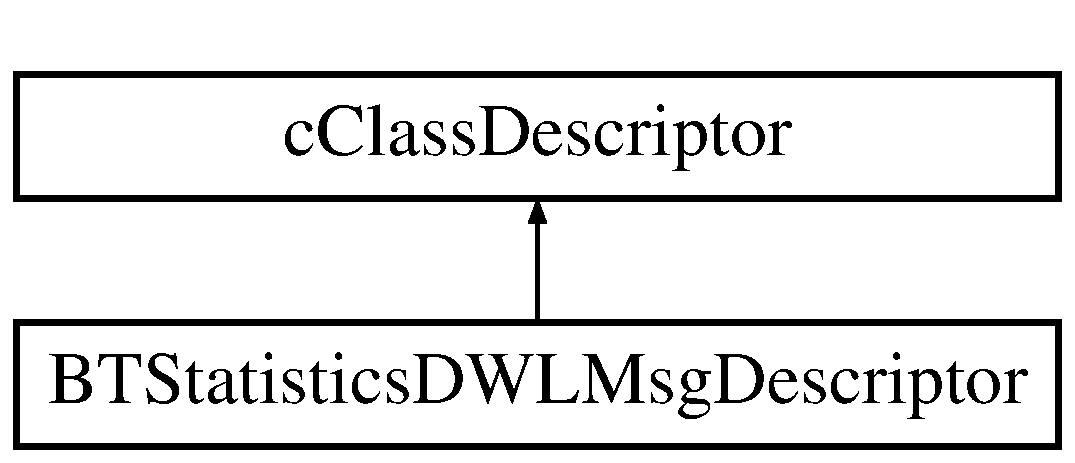
\includegraphics[height=2.000000cm]{classBTStatisticsDWLMsgDescriptor}
\end{center}
\end{figure}
\subsection*{Public Member Functions}
\begin{DoxyCompactItemize}
\item 
\hyperlink{classBTStatisticsDWLMsgDescriptor_afd2006c8f12e6834e6c8cfb671171fbb}{B\+T\+Statistics\+D\+W\+L\+Msg\+Descriptor} ()
\item 
virtual \hyperlink{classBTStatisticsDWLMsgDescriptor_a7abbf3f34f30439df097934b883f9b39}{$\sim$\+B\+T\+Statistics\+D\+W\+L\+Msg\+Descriptor} ()
\item 
virtual bool \hyperlink{classBTStatisticsDWLMsgDescriptor_acb74af73cc5d8edcb8c518e5d7ab559d}{does\+Support} (c\+Object $\ast$obj) const 
\item 
virtual const char $\ast$ \hyperlink{classBTStatisticsDWLMsgDescriptor_a72de611deef990b2e9cbdfd82cdd2db8}{get\+Property} (const char $\ast$propertyname) const 
\item 
virtual int \hyperlink{classBTStatisticsDWLMsgDescriptor_a52aea50bbf9dcec7aa47d401d2ade3bc}{get\+Field\+Count} (void $\ast$object) const 
\item 
virtual const char $\ast$ \hyperlink{classBTStatisticsDWLMsgDescriptor_accc1015d4347e58ad0e1b8634cadee5d}{get\+Field\+Name} (void $\ast$object, int field) const 
\item 
virtual int \hyperlink{classBTStatisticsDWLMsgDescriptor_afc632a1b0180b4b6f703876e8694be9f}{find\+Field} (void $\ast$object, const char $\ast$field\+Name) const 
\item 
virtual unsigned int \hyperlink{classBTStatisticsDWLMsgDescriptor_ab21541c25650b6c170be89339c3ad214}{get\+Field\+Type\+Flags} (void $\ast$object, int field) const 
\item 
virtual const char $\ast$ \hyperlink{classBTStatisticsDWLMsgDescriptor_afa150f1ad321846d46ee09190e3baba4}{get\+Field\+Type\+String} (void $\ast$object, int field) const 
\item 
virtual const char $\ast$ \hyperlink{classBTStatisticsDWLMsgDescriptor_a267a3e6b4aef2e62201a58c12d53571a}{get\+Field\+Property} (void $\ast$object, int field, const char $\ast$propertyname) const 
\item 
virtual int \hyperlink{classBTStatisticsDWLMsgDescriptor_a19efa81b95145202070413793ab53f81}{get\+Array\+Size} (void $\ast$object, int field) const 
\item 
virtual std\+::string \hyperlink{classBTStatisticsDWLMsgDescriptor_aaed50886a0630ee5626df39e794828bd}{get\+Field\+As\+String} (void $\ast$object, int field, int i) const 
\item 
virtual bool \hyperlink{classBTStatisticsDWLMsgDescriptor_a946a7270b8d23e85b57dbed35e1e33a2}{set\+Field\+As\+String} (void $\ast$object, int field, int i, const char $\ast$value) const 
\item 
virtual const char $\ast$ \hyperlink{classBTStatisticsDWLMsgDescriptor_a9bf18cbeb0727a6821097256f26edf65}{get\+Field\+Struct\+Name} (void $\ast$object, int field) const 
\item 
virtual void $\ast$ \hyperlink{classBTStatisticsDWLMsgDescriptor_adda69865e339b65ec9402d4db4eb3134}{get\+Field\+Struct\+Pointer} (void $\ast$object, int field, int i) const 
\end{DoxyCompactItemize}


\subsection{Constructor \& Destructor Documentation}
\hypertarget{classBTStatisticsDWLMsgDescriptor_afd2006c8f12e6834e6c8cfb671171fbb}{}\index{B\+T\+Statistics\+D\+W\+L\+Msg\+Descriptor@{B\+T\+Statistics\+D\+W\+L\+Msg\+Descriptor}!B\+T\+Statistics\+D\+W\+L\+Msg\+Descriptor@{B\+T\+Statistics\+D\+W\+L\+Msg\+Descriptor}}
\index{B\+T\+Statistics\+D\+W\+L\+Msg\+Descriptor@{B\+T\+Statistics\+D\+W\+L\+Msg\+Descriptor}!B\+T\+Statistics\+D\+W\+L\+Msg\+Descriptor@{B\+T\+Statistics\+D\+W\+L\+Msg\+Descriptor}}
\subsubsection[{B\+T\+Statistics\+D\+W\+L\+Msg\+Descriptor()}]{\setlength{\rightskip}{0pt plus 5cm}B\+T\+Statistics\+D\+W\+L\+Msg\+Descriptor\+::\+B\+T\+Statistics\+D\+W\+L\+Msg\+Descriptor (
\begin{DoxyParamCaption}
{}
\end{DoxyParamCaption}
)}\label{classBTStatisticsDWLMsgDescriptor_afd2006c8f12e6834e6c8cfb671171fbb}
\hypertarget{classBTStatisticsDWLMsgDescriptor_a7abbf3f34f30439df097934b883f9b39}{}\index{B\+T\+Statistics\+D\+W\+L\+Msg\+Descriptor@{B\+T\+Statistics\+D\+W\+L\+Msg\+Descriptor}!````~B\+T\+Statistics\+D\+W\+L\+Msg\+Descriptor@{$\sim$\+B\+T\+Statistics\+D\+W\+L\+Msg\+Descriptor}}
\index{````~B\+T\+Statistics\+D\+W\+L\+Msg\+Descriptor@{$\sim$\+B\+T\+Statistics\+D\+W\+L\+Msg\+Descriptor}!B\+T\+Statistics\+D\+W\+L\+Msg\+Descriptor@{B\+T\+Statistics\+D\+W\+L\+Msg\+Descriptor}}
\subsubsection[{$\sim$\+B\+T\+Statistics\+D\+W\+L\+Msg\+Descriptor()}]{\setlength{\rightskip}{0pt plus 5cm}B\+T\+Statistics\+D\+W\+L\+Msg\+Descriptor\+::$\sim$\+B\+T\+Statistics\+D\+W\+L\+Msg\+Descriptor (
\begin{DoxyParamCaption}
{}
\end{DoxyParamCaption}
)\hspace{0.3cm}{\ttfamily [virtual]}}\label{classBTStatisticsDWLMsgDescriptor_a7abbf3f34f30439df097934b883f9b39}


\subsection{Member Function Documentation}
\hypertarget{classBTStatisticsDWLMsgDescriptor_acb74af73cc5d8edcb8c518e5d7ab559d}{}\index{B\+T\+Statistics\+D\+W\+L\+Msg\+Descriptor@{B\+T\+Statistics\+D\+W\+L\+Msg\+Descriptor}!does\+Support@{does\+Support}}
\index{does\+Support@{does\+Support}!B\+T\+Statistics\+D\+W\+L\+Msg\+Descriptor@{B\+T\+Statistics\+D\+W\+L\+Msg\+Descriptor}}
\subsubsection[{does\+Support(c\+Object $\ast$obj) const }]{\setlength{\rightskip}{0pt plus 5cm}bool B\+T\+Statistics\+D\+W\+L\+Msg\+Descriptor\+::does\+Support (
\begin{DoxyParamCaption}
\item[{c\+Object $\ast$}]{obj}
\end{DoxyParamCaption}
) const\hspace{0.3cm}{\ttfamily [virtual]}}\label{classBTStatisticsDWLMsgDescriptor_acb74af73cc5d8edcb8c518e5d7ab559d}
\hypertarget{classBTStatisticsDWLMsgDescriptor_afc632a1b0180b4b6f703876e8694be9f}{}\index{B\+T\+Statistics\+D\+W\+L\+Msg\+Descriptor@{B\+T\+Statistics\+D\+W\+L\+Msg\+Descriptor}!find\+Field@{find\+Field}}
\index{find\+Field@{find\+Field}!B\+T\+Statistics\+D\+W\+L\+Msg\+Descriptor@{B\+T\+Statistics\+D\+W\+L\+Msg\+Descriptor}}
\subsubsection[{find\+Field(void $\ast$object, const char $\ast$field\+Name) const }]{\setlength{\rightskip}{0pt plus 5cm}int B\+T\+Statistics\+D\+W\+L\+Msg\+Descriptor\+::find\+Field (
\begin{DoxyParamCaption}
\item[{void $\ast$}]{object, }
\item[{const char $\ast$}]{field\+Name}
\end{DoxyParamCaption}
) const\hspace{0.3cm}{\ttfamily [virtual]}}\label{classBTStatisticsDWLMsgDescriptor_afc632a1b0180b4b6f703876e8694be9f}
\hypertarget{classBTStatisticsDWLMsgDescriptor_a19efa81b95145202070413793ab53f81}{}\index{B\+T\+Statistics\+D\+W\+L\+Msg\+Descriptor@{B\+T\+Statistics\+D\+W\+L\+Msg\+Descriptor}!get\+Array\+Size@{get\+Array\+Size}}
\index{get\+Array\+Size@{get\+Array\+Size}!B\+T\+Statistics\+D\+W\+L\+Msg\+Descriptor@{B\+T\+Statistics\+D\+W\+L\+Msg\+Descriptor}}
\subsubsection[{get\+Array\+Size(void $\ast$object, int field) const }]{\setlength{\rightskip}{0pt plus 5cm}int B\+T\+Statistics\+D\+W\+L\+Msg\+Descriptor\+::get\+Array\+Size (
\begin{DoxyParamCaption}
\item[{void $\ast$}]{object, }
\item[{int}]{field}
\end{DoxyParamCaption}
) const\hspace{0.3cm}{\ttfamily [virtual]}}\label{classBTStatisticsDWLMsgDescriptor_a19efa81b95145202070413793ab53f81}
\hypertarget{classBTStatisticsDWLMsgDescriptor_aaed50886a0630ee5626df39e794828bd}{}\index{B\+T\+Statistics\+D\+W\+L\+Msg\+Descriptor@{B\+T\+Statistics\+D\+W\+L\+Msg\+Descriptor}!get\+Field\+As\+String@{get\+Field\+As\+String}}
\index{get\+Field\+As\+String@{get\+Field\+As\+String}!B\+T\+Statistics\+D\+W\+L\+Msg\+Descriptor@{B\+T\+Statistics\+D\+W\+L\+Msg\+Descriptor}}
\subsubsection[{get\+Field\+As\+String(void $\ast$object, int field, int i) const }]{\setlength{\rightskip}{0pt plus 5cm}std\+::string B\+T\+Statistics\+D\+W\+L\+Msg\+Descriptor\+::get\+Field\+As\+String (
\begin{DoxyParamCaption}
\item[{void $\ast$}]{object, }
\item[{int}]{field, }
\item[{int}]{i}
\end{DoxyParamCaption}
) const\hspace{0.3cm}{\ttfamily [virtual]}}\label{classBTStatisticsDWLMsgDescriptor_aaed50886a0630ee5626df39e794828bd}
\hypertarget{classBTStatisticsDWLMsgDescriptor_a52aea50bbf9dcec7aa47d401d2ade3bc}{}\index{B\+T\+Statistics\+D\+W\+L\+Msg\+Descriptor@{B\+T\+Statistics\+D\+W\+L\+Msg\+Descriptor}!get\+Field\+Count@{get\+Field\+Count}}
\index{get\+Field\+Count@{get\+Field\+Count}!B\+T\+Statistics\+D\+W\+L\+Msg\+Descriptor@{B\+T\+Statistics\+D\+W\+L\+Msg\+Descriptor}}
\subsubsection[{get\+Field\+Count(void $\ast$object) const }]{\setlength{\rightskip}{0pt plus 5cm}int B\+T\+Statistics\+D\+W\+L\+Msg\+Descriptor\+::get\+Field\+Count (
\begin{DoxyParamCaption}
\item[{void $\ast$}]{object}
\end{DoxyParamCaption}
) const\hspace{0.3cm}{\ttfamily [virtual]}}\label{classBTStatisticsDWLMsgDescriptor_a52aea50bbf9dcec7aa47d401d2ade3bc}
\hypertarget{classBTStatisticsDWLMsgDescriptor_accc1015d4347e58ad0e1b8634cadee5d}{}\index{B\+T\+Statistics\+D\+W\+L\+Msg\+Descriptor@{B\+T\+Statistics\+D\+W\+L\+Msg\+Descriptor}!get\+Field\+Name@{get\+Field\+Name}}
\index{get\+Field\+Name@{get\+Field\+Name}!B\+T\+Statistics\+D\+W\+L\+Msg\+Descriptor@{B\+T\+Statistics\+D\+W\+L\+Msg\+Descriptor}}
\subsubsection[{get\+Field\+Name(void $\ast$object, int field) const }]{\setlength{\rightskip}{0pt plus 5cm}const char $\ast$ B\+T\+Statistics\+D\+W\+L\+Msg\+Descriptor\+::get\+Field\+Name (
\begin{DoxyParamCaption}
\item[{void $\ast$}]{object, }
\item[{int}]{field}
\end{DoxyParamCaption}
) const\hspace{0.3cm}{\ttfamily [virtual]}}\label{classBTStatisticsDWLMsgDescriptor_accc1015d4347e58ad0e1b8634cadee5d}
\hypertarget{classBTStatisticsDWLMsgDescriptor_a267a3e6b4aef2e62201a58c12d53571a}{}\index{B\+T\+Statistics\+D\+W\+L\+Msg\+Descriptor@{B\+T\+Statistics\+D\+W\+L\+Msg\+Descriptor}!get\+Field\+Property@{get\+Field\+Property}}
\index{get\+Field\+Property@{get\+Field\+Property}!B\+T\+Statistics\+D\+W\+L\+Msg\+Descriptor@{B\+T\+Statistics\+D\+W\+L\+Msg\+Descriptor}}
\subsubsection[{get\+Field\+Property(void $\ast$object, int field, const char $\ast$propertyname) const }]{\setlength{\rightskip}{0pt plus 5cm}const char $\ast$ B\+T\+Statistics\+D\+W\+L\+Msg\+Descriptor\+::get\+Field\+Property (
\begin{DoxyParamCaption}
\item[{void $\ast$}]{object, }
\item[{int}]{field, }
\item[{const char $\ast$}]{propertyname}
\end{DoxyParamCaption}
) const\hspace{0.3cm}{\ttfamily [virtual]}}\label{classBTStatisticsDWLMsgDescriptor_a267a3e6b4aef2e62201a58c12d53571a}
\hypertarget{classBTStatisticsDWLMsgDescriptor_a9bf18cbeb0727a6821097256f26edf65}{}\index{B\+T\+Statistics\+D\+W\+L\+Msg\+Descriptor@{B\+T\+Statistics\+D\+W\+L\+Msg\+Descriptor}!get\+Field\+Struct\+Name@{get\+Field\+Struct\+Name}}
\index{get\+Field\+Struct\+Name@{get\+Field\+Struct\+Name}!B\+T\+Statistics\+D\+W\+L\+Msg\+Descriptor@{B\+T\+Statistics\+D\+W\+L\+Msg\+Descriptor}}
\subsubsection[{get\+Field\+Struct\+Name(void $\ast$object, int field) const }]{\setlength{\rightskip}{0pt plus 5cm}const char $\ast$ B\+T\+Statistics\+D\+W\+L\+Msg\+Descriptor\+::get\+Field\+Struct\+Name (
\begin{DoxyParamCaption}
\item[{void $\ast$}]{object, }
\item[{int}]{field}
\end{DoxyParamCaption}
) const\hspace{0.3cm}{\ttfamily [virtual]}}\label{classBTStatisticsDWLMsgDescriptor_a9bf18cbeb0727a6821097256f26edf65}
\hypertarget{classBTStatisticsDWLMsgDescriptor_adda69865e339b65ec9402d4db4eb3134}{}\index{B\+T\+Statistics\+D\+W\+L\+Msg\+Descriptor@{B\+T\+Statistics\+D\+W\+L\+Msg\+Descriptor}!get\+Field\+Struct\+Pointer@{get\+Field\+Struct\+Pointer}}
\index{get\+Field\+Struct\+Pointer@{get\+Field\+Struct\+Pointer}!B\+T\+Statistics\+D\+W\+L\+Msg\+Descriptor@{B\+T\+Statistics\+D\+W\+L\+Msg\+Descriptor}}
\subsubsection[{get\+Field\+Struct\+Pointer(void $\ast$object, int field, int i) const }]{\setlength{\rightskip}{0pt plus 5cm}void $\ast$ B\+T\+Statistics\+D\+W\+L\+Msg\+Descriptor\+::get\+Field\+Struct\+Pointer (
\begin{DoxyParamCaption}
\item[{void $\ast$}]{object, }
\item[{int}]{field, }
\item[{int}]{i}
\end{DoxyParamCaption}
) const\hspace{0.3cm}{\ttfamily [virtual]}}\label{classBTStatisticsDWLMsgDescriptor_adda69865e339b65ec9402d4db4eb3134}
\hypertarget{classBTStatisticsDWLMsgDescriptor_ab21541c25650b6c170be89339c3ad214}{}\index{B\+T\+Statistics\+D\+W\+L\+Msg\+Descriptor@{B\+T\+Statistics\+D\+W\+L\+Msg\+Descriptor}!get\+Field\+Type\+Flags@{get\+Field\+Type\+Flags}}
\index{get\+Field\+Type\+Flags@{get\+Field\+Type\+Flags}!B\+T\+Statistics\+D\+W\+L\+Msg\+Descriptor@{B\+T\+Statistics\+D\+W\+L\+Msg\+Descriptor}}
\subsubsection[{get\+Field\+Type\+Flags(void $\ast$object, int field) const }]{\setlength{\rightskip}{0pt plus 5cm}unsigned int B\+T\+Statistics\+D\+W\+L\+Msg\+Descriptor\+::get\+Field\+Type\+Flags (
\begin{DoxyParamCaption}
\item[{void $\ast$}]{object, }
\item[{int}]{field}
\end{DoxyParamCaption}
) const\hspace{0.3cm}{\ttfamily [virtual]}}\label{classBTStatisticsDWLMsgDescriptor_ab21541c25650b6c170be89339c3ad214}
\hypertarget{classBTStatisticsDWLMsgDescriptor_afa150f1ad321846d46ee09190e3baba4}{}\index{B\+T\+Statistics\+D\+W\+L\+Msg\+Descriptor@{B\+T\+Statistics\+D\+W\+L\+Msg\+Descriptor}!get\+Field\+Type\+String@{get\+Field\+Type\+String}}
\index{get\+Field\+Type\+String@{get\+Field\+Type\+String}!B\+T\+Statistics\+D\+W\+L\+Msg\+Descriptor@{B\+T\+Statistics\+D\+W\+L\+Msg\+Descriptor}}
\subsubsection[{get\+Field\+Type\+String(void $\ast$object, int field) const }]{\setlength{\rightskip}{0pt plus 5cm}const char $\ast$ B\+T\+Statistics\+D\+W\+L\+Msg\+Descriptor\+::get\+Field\+Type\+String (
\begin{DoxyParamCaption}
\item[{void $\ast$}]{object, }
\item[{int}]{field}
\end{DoxyParamCaption}
) const\hspace{0.3cm}{\ttfamily [virtual]}}\label{classBTStatisticsDWLMsgDescriptor_afa150f1ad321846d46ee09190e3baba4}
\hypertarget{classBTStatisticsDWLMsgDescriptor_a72de611deef990b2e9cbdfd82cdd2db8}{}\index{B\+T\+Statistics\+D\+W\+L\+Msg\+Descriptor@{B\+T\+Statistics\+D\+W\+L\+Msg\+Descriptor}!get\+Property@{get\+Property}}
\index{get\+Property@{get\+Property}!B\+T\+Statistics\+D\+W\+L\+Msg\+Descriptor@{B\+T\+Statistics\+D\+W\+L\+Msg\+Descriptor}}
\subsubsection[{get\+Property(const char $\ast$propertyname) const }]{\setlength{\rightskip}{0pt plus 5cm}const char $\ast$ B\+T\+Statistics\+D\+W\+L\+Msg\+Descriptor\+::get\+Property (
\begin{DoxyParamCaption}
\item[{const char $\ast$}]{propertyname}
\end{DoxyParamCaption}
) const\hspace{0.3cm}{\ttfamily [virtual]}}\label{classBTStatisticsDWLMsgDescriptor_a72de611deef990b2e9cbdfd82cdd2db8}
\hypertarget{classBTStatisticsDWLMsgDescriptor_a946a7270b8d23e85b57dbed35e1e33a2}{}\index{B\+T\+Statistics\+D\+W\+L\+Msg\+Descriptor@{B\+T\+Statistics\+D\+W\+L\+Msg\+Descriptor}!set\+Field\+As\+String@{set\+Field\+As\+String}}
\index{set\+Field\+As\+String@{set\+Field\+As\+String}!B\+T\+Statistics\+D\+W\+L\+Msg\+Descriptor@{B\+T\+Statistics\+D\+W\+L\+Msg\+Descriptor}}
\subsubsection[{set\+Field\+As\+String(void $\ast$object, int field, int i, const char $\ast$value) const }]{\setlength{\rightskip}{0pt plus 5cm}bool B\+T\+Statistics\+D\+W\+L\+Msg\+Descriptor\+::set\+Field\+As\+String (
\begin{DoxyParamCaption}
\item[{void $\ast$}]{object, }
\item[{int}]{field, }
\item[{int}]{i, }
\item[{const char $\ast$}]{value}
\end{DoxyParamCaption}
) const\hspace{0.3cm}{\ttfamily [virtual]}}\label{classBTStatisticsDWLMsgDescriptor_a946a7270b8d23e85b57dbed35e1e33a2}


The documentation for this class was generated from the following file\+:\begin{DoxyCompactItemize}
\item 
\hyperlink{BTStatisticsMsg__m_8cc}{B\+T\+Statistics\+Msg\+\_\+m.\+cc}\end{DoxyCompactItemize}

\hypertarget{classBTStatisticsNumHitsMsg}{}\section{B\+T\+Statistics\+Num\+Hits\+Msg Class Reference}
\label{classBTStatisticsNumHitsMsg}\index{B\+T\+Statistics\+Num\+Hits\+Msg@{B\+T\+Statistics\+Num\+Hits\+Msg}}


{\ttfamily \#include $<$B\+T\+Statistics\+Msg\+\_\+m.\+h$>$}

Inheritance diagram for B\+T\+Statistics\+Num\+Hits\+Msg\+:\begin{figure}[H]
\begin{center}
\leavevmode
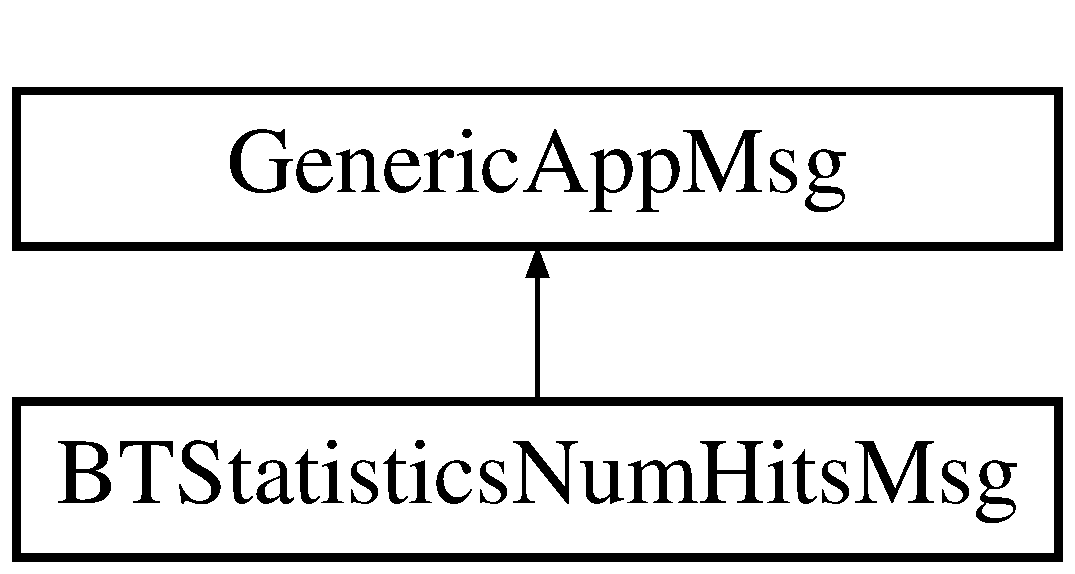
\includegraphics[height=2.000000cm]{classBTStatisticsNumHitsMsg}
\end{center}
\end{figure}
\subsection*{Public Member Functions}
\begin{DoxyCompactItemize}
\item 
\hyperlink{classBTStatisticsNumHitsMsg_a48a37fdce2832cda8c98f6864a602464}{B\+T\+Statistics\+Num\+Hits\+Msg} (const char $\ast$name=N\+U\+L\+L, int kind=0)
\item 
\hyperlink{classBTStatisticsNumHitsMsg_ab6d8b31a3fc613f9d6400f869dfc8532}{B\+T\+Statistics\+Num\+Hits\+Msg} (const \hyperlink{classBTStatisticsNumHitsMsg}{B\+T\+Statistics\+Num\+Hits\+Msg} \&other)
\item 
virtual \hyperlink{classBTStatisticsNumHitsMsg_afb330a4e351d76177965e09d8fd52c7c}{$\sim$\+B\+T\+Statistics\+Num\+Hits\+Msg} ()
\item 
\hyperlink{classBTStatisticsNumHitsMsg}{B\+T\+Statistics\+Num\+Hits\+Msg} \& \hyperlink{classBTStatisticsNumHitsMsg_a74b35dfa26a72be8faf9334103913286}{operator=} (const \hyperlink{classBTStatisticsNumHitsMsg}{B\+T\+Statistics\+Num\+Hits\+Msg} \&other)
\item 
virtual \hyperlink{classBTStatisticsNumHitsMsg}{B\+T\+Statistics\+Num\+Hits\+Msg} $\ast$ \hyperlink{classBTStatisticsNumHitsMsg_a74abfdee89f6fd590ba930534ece7a60}{dup} () const 
\item 
virtual void \hyperlink{classBTStatisticsNumHitsMsg_aad9ededcecb9b2fcae86683baa48851c}{parsim\+Pack} (c\+Comm\+Buffer $\ast$b)
\item 
virtual void \hyperlink{classBTStatisticsNumHitsMsg_a28ce087da02b0d989b2120274e6e660c}{parsim\+Unpack} (c\+Comm\+Buffer $\ast$b)
\item 
virtual double \hyperlink{classBTStatisticsNumHitsMsg_ada909e3fd93e099cb0ec5c25fca1047c}{num\+Hits} () const 
\item 
virtual void \hyperlink{classBTStatisticsNumHitsMsg_af0a902e211d083fbd601a0d6f6939c7d}{set\+Num\+Hits} (double \hyperlink{classBTStatisticsNumHitsMsg_a88f5611c41dac9956bc6a07fe15f28eb}{num\+Hits\+\_\+var})
\end{DoxyCompactItemize}
\subsection*{Protected Member Functions}
\begin{DoxyCompactItemize}
\item 
bool \hyperlink{classBTStatisticsNumHitsMsg_ab81878625fc5d4d3b9be33811da01e8e}{operator==} (const \hyperlink{classBTStatisticsNumHitsMsg}{B\+T\+Statistics\+Num\+Hits\+Msg} \&)
\end{DoxyCompactItemize}
\subsection*{Protected Attributes}
\begin{DoxyCompactItemize}
\item 
double \hyperlink{classBTStatisticsNumHitsMsg_a88f5611c41dac9956bc6a07fe15f28eb}{num\+Hits\+\_\+var}
\end{DoxyCompactItemize}


\subsection{Detailed Description}
Class generated from {\ttfamily applications/x\+Bit\+Torrent/\+B\+T\+Statistics\+Msg.\+msg} by opp\+\_\+msgc. 
\begin{DoxyPre}
message \hyperlink{classBTStatisticsNumHitsMsg}{BTStatisticsNumHitsMsg} extends GenericAppMsg
\{
     (true);\end{DoxyPre}



\begin{DoxyPre}    double numHits;
\}
\end{DoxyPre}
 

\subsection{Constructor \& Destructor Documentation}
\hypertarget{classBTStatisticsNumHitsMsg_a48a37fdce2832cda8c98f6864a602464}{}\index{B\+T\+Statistics\+Num\+Hits\+Msg@{B\+T\+Statistics\+Num\+Hits\+Msg}!B\+T\+Statistics\+Num\+Hits\+Msg@{B\+T\+Statistics\+Num\+Hits\+Msg}}
\index{B\+T\+Statistics\+Num\+Hits\+Msg@{B\+T\+Statistics\+Num\+Hits\+Msg}!B\+T\+Statistics\+Num\+Hits\+Msg@{B\+T\+Statistics\+Num\+Hits\+Msg}}
\subsubsection[{B\+T\+Statistics\+Num\+Hits\+Msg(const char $\ast$name=\+N\+U\+L\+L, int kind=0)}]{\setlength{\rightskip}{0pt plus 5cm}B\+T\+Statistics\+Num\+Hits\+Msg\+::\+B\+T\+Statistics\+Num\+Hits\+Msg (
\begin{DoxyParamCaption}
\item[{const char $\ast$}]{name = {\ttfamily NULL}, }
\item[{int}]{kind = {\ttfamily 0}}
\end{DoxyParamCaption}
)}\label{classBTStatisticsNumHitsMsg_a48a37fdce2832cda8c98f6864a602464}
\hypertarget{classBTStatisticsNumHitsMsg_ab6d8b31a3fc613f9d6400f869dfc8532}{}\index{B\+T\+Statistics\+Num\+Hits\+Msg@{B\+T\+Statistics\+Num\+Hits\+Msg}!B\+T\+Statistics\+Num\+Hits\+Msg@{B\+T\+Statistics\+Num\+Hits\+Msg}}
\index{B\+T\+Statistics\+Num\+Hits\+Msg@{B\+T\+Statistics\+Num\+Hits\+Msg}!B\+T\+Statistics\+Num\+Hits\+Msg@{B\+T\+Statistics\+Num\+Hits\+Msg}}
\subsubsection[{B\+T\+Statistics\+Num\+Hits\+Msg(const B\+T\+Statistics\+Num\+Hits\+Msg \&other)}]{\setlength{\rightskip}{0pt plus 5cm}B\+T\+Statistics\+Num\+Hits\+Msg\+::\+B\+T\+Statistics\+Num\+Hits\+Msg (
\begin{DoxyParamCaption}
\item[{const {\bf B\+T\+Statistics\+Num\+Hits\+Msg} \&}]{other}
\end{DoxyParamCaption}
)}\label{classBTStatisticsNumHitsMsg_ab6d8b31a3fc613f9d6400f869dfc8532}
\hypertarget{classBTStatisticsNumHitsMsg_afb330a4e351d76177965e09d8fd52c7c}{}\index{B\+T\+Statistics\+Num\+Hits\+Msg@{B\+T\+Statistics\+Num\+Hits\+Msg}!````~B\+T\+Statistics\+Num\+Hits\+Msg@{$\sim$\+B\+T\+Statistics\+Num\+Hits\+Msg}}
\index{````~B\+T\+Statistics\+Num\+Hits\+Msg@{$\sim$\+B\+T\+Statistics\+Num\+Hits\+Msg}!B\+T\+Statistics\+Num\+Hits\+Msg@{B\+T\+Statistics\+Num\+Hits\+Msg}}
\subsubsection[{$\sim$\+B\+T\+Statistics\+Num\+Hits\+Msg()}]{\setlength{\rightskip}{0pt plus 5cm}B\+T\+Statistics\+Num\+Hits\+Msg\+::$\sim$\+B\+T\+Statistics\+Num\+Hits\+Msg (
\begin{DoxyParamCaption}
{}
\end{DoxyParamCaption}
)\hspace{0.3cm}{\ttfamily [virtual]}}\label{classBTStatisticsNumHitsMsg_afb330a4e351d76177965e09d8fd52c7c}


\subsection{Member Function Documentation}
\hypertarget{classBTStatisticsNumHitsMsg_a74abfdee89f6fd590ba930534ece7a60}{}\index{B\+T\+Statistics\+Num\+Hits\+Msg@{B\+T\+Statistics\+Num\+Hits\+Msg}!dup@{dup}}
\index{dup@{dup}!B\+T\+Statistics\+Num\+Hits\+Msg@{B\+T\+Statistics\+Num\+Hits\+Msg}}
\subsubsection[{dup() const }]{\setlength{\rightskip}{0pt plus 5cm}virtual {\bf B\+T\+Statistics\+Num\+Hits\+Msg}$\ast$ B\+T\+Statistics\+Num\+Hits\+Msg\+::dup (
\begin{DoxyParamCaption}
{}
\end{DoxyParamCaption}
) const\hspace{0.3cm}{\ttfamily [inline]}, {\ttfamily [virtual]}}\label{classBTStatisticsNumHitsMsg_a74abfdee89f6fd590ba930534ece7a60}
\hypertarget{classBTStatisticsNumHitsMsg_ada909e3fd93e099cb0ec5c25fca1047c}{}\index{B\+T\+Statistics\+Num\+Hits\+Msg@{B\+T\+Statistics\+Num\+Hits\+Msg}!num\+Hits@{num\+Hits}}
\index{num\+Hits@{num\+Hits}!B\+T\+Statistics\+Num\+Hits\+Msg@{B\+T\+Statistics\+Num\+Hits\+Msg}}
\subsubsection[{num\+Hits() const }]{\setlength{\rightskip}{0pt plus 5cm}double B\+T\+Statistics\+Num\+Hits\+Msg\+::num\+Hits (
\begin{DoxyParamCaption}
{}
\end{DoxyParamCaption}
) const\hspace{0.3cm}{\ttfamily [virtual]}}\label{classBTStatisticsNumHitsMsg_ada909e3fd93e099cb0ec5c25fca1047c}
\hypertarget{classBTStatisticsNumHitsMsg_a74b35dfa26a72be8faf9334103913286}{}\index{B\+T\+Statistics\+Num\+Hits\+Msg@{B\+T\+Statistics\+Num\+Hits\+Msg}!operator=@{operator=}}
\index{operator=@{operator=}!B\+T\+Statistics\+Num\+Hits\+Msg@{B\+T\+Statistics\+Num\+Hits\+Msg}}
\subsubsection[{operator=(const B\+T\+Statistics\+Num\+Hits\+Msg \&other)}]{\setlength{\rightskip}{0pt plus 5cm}{\bf B\+T\+Statistics\+Num\+Hits\+Msg} \& B\+T\+Statistics\+Num\+Hits\+Msg\+::operator= (
\begin{DoxyParamCaption}
\item[{const {\bf B\+T\+Statistics\+Num\+Hits\+Msg} \&}]{other}
\end{DoxyParamCaption}
)}\label{classBTStatisticsNumHitsMsg_a74b35dfa26a72be8faf9334103913286}
\hypertarget{classBTStatisticsNumHitsMsg_ab81878625fc5d4d3b9be33811da01e8e}{}\index{B\+T\+Statistics\+Num\+Hits\+Msg@{B\+T\+Statistics\+Num\+Hits\+Msg}!operator==@{operator==}}
\index{operator==@{operator==}!B\+T\+Statistics\+Num\+Hits\+Msg@{B\+T\+Statistics\+Num\+Hits\+Msg}}
\subsubsection[{operator==(const B\+T\+Statistics\+Num\+Hits\+Msg \&)}]{\setlength{\rightskip}{0pt plus 5cm}bool B\+T\+Statistics\+Num\+Hits\+Msg\+::operator== (
\begin{DoxyParamCaption}
\item[{const {\bf B\+T\+Statistics\+Num\+Hits\+Msg} \&}]{}
\end{DoxyParamCaption}
)\hspace{0.3cm}{\ttfamily [protected]}}\label{classBTStatisticsNumHitsMsg_ab81878625fc5d4d3b9be33811da01e8e}
\hypertarget{classBTStatisticsNumHitsMsg_aad9ededcecb9b2fcae86683baa48851c}{}\index{B\+T\+Statistics\+Num\+Hits\+Msg@{B\+T\+Statistics\+Num\+Hits\+Msg}!parsim\+Pack@{parsim\+Pack}}
\index{parsim\+Pack@{parsim\+Pack}!B\+T\+Statistics\+Num\+Hits\+Msg@{B\+T\+Statistics\+Num\+Hits\+Msg}}
\subsubsection[{parsim\+Pack(c\+Comm\+Buffer $\ast$b)}]{\setlength{\rightskip}{0pt plus 5cm}void B\+T\+Statistics\+Num\+Hits\+Msg\+::parsim\+Pack (
\begin{DoxyParamCaption}
\item[{c\+Comm\+Buffer $\ast$}]{b}
\end{DoxyParamCaption}
)\hspace{0.3cm}{\ttfamily [virtual]}}\label{classBTStatisticsNumHitsMsg_aad9ededcecb9b2fcae86683baa48851c}
\hypertarget{classBTStatisticsNumHitsMsg_a28ce087da02b0d989b2120274e6e660c}{}\index{B\+T\+Statistics\+Num\+Hits\+Msg@{B\+T\+Statistics\+Num\+Hits\+Msg}!parsim\+Unpack@{parsim\+Unpack}}
\index{parsim\+Unpack@{parsim\+Unpack}!B\+T\+Statistics\+Num\+Hits\+Msg@{B\+T\+Statistics\+Num\+Hits\+Msg}}
\subsubsection[{parsim\+Unpack(c\+Comm\+Buffer $\ast$b)}]{\setlength{\rightskip}{0pt plus 5cm}void B\+T\+Statistics\+Num\+Hits\+Msg\+::parsim\+Unpack (
\begin{DoxyParamCaption}
\item[{c\+Comm\+Buffer $\ast$}]{b}
\end{DoxyParamCaption}
)\hspace{0.3cm}{\ttfamily [virtual]}}\label{classBTStatisticsNumHitsMsg_a28ce087da02b0d989b2120274e6e660c}
\hypertarget{classBTStatisticsNumHitsMsg_af0a902e211d083fbd601a0d6f6939c7d}{}\index{B\+T\+Statistics\+Num\+Hits\+Msg@{B\+T\+Statistics\+Num\+Hits\+Msg}!set\+Num\+Hits@{set\+Num\+Hits}}
\index{set\+Num\+Hits@{set\+Num\+Hits}!B\+T\+Statistics\+Num\+Hits\+Msg@{B\+T\+Statistics\+Num\+Hits\+Msg}}
\subsubsection[{set\+Num\+Hits(double num\+Hits\+\_\+var)}]{\setlength{\rightskip}{0pt plus 5cm}void B\+T\+Statistics\+Num\+Hits\+Msg\+::set\+Num\+Hits (
\begin{DoxyParamCaption}
\item[{double}]{num\+Hits\+\_\+var}
\end{DoxyParamCaption}
)\hspace{0.3cm}{\ttfamily [virtual]}}\label{classBTStatisticsNumHitsMsg_af0a902e211d083fbd601a0d6f6939c7d}


\subsection{Member Data Documentation}
\hypertarget{classBTStatisticsNumHitsMsg_a88f5611c41dac9956bc6a07fe15f28eb}{}\index{B\+T\+Statistics\+Num\+Hits\+Msg@{B\+T\+Statistics\+Num\+Hits\+Msg}!num\+Hits\+\_\+var@{num\+Hits\+\_\+var}}
\index{num\+Hits\+\_\+var@{num\+Hits\+\_\+var}!B\+T\+Statistics\+Num\+Hits\+Msg@{B\+T\+Statistics\+Num\+Hits\+Msg}}
\subsubsection[{num\+Hits\+\_\+var}]{\setlength{\rightskip}{0pt plus 5cm}double B\+T\+Statistics\+Num\+Hits\+Msg\+::num\+Hits\+\_\+var\hspace{0.3cm}{\ttfamily [protected]}}\label{classBTStatisticsNumHitsMsg_a88f5611c41dac9956bc6a07fe15f28eb}


The documentation for this class was generated from the following files\+:\begin{DoxyCompactItemize}
\item 
\hyperlink{BTStatisticsMsg__m_8h}{B\+T\+Statistics\+Msg\+\_\+m.\+h}\item 
\hyperlink{BTStatisticsMsg__m_8cc}{B\+T\+Statistics\+Msg\+\_\+m.\+cc}\end{DoxyCompactItemize}

\hypertarget{classBTStatisticsNumHitsMsgDescriptor}{}\section{B\+T\+Statistics\+Num\+Hits\+Msg\+Descriptor Class Reference}
\label{classBTStatisticsNumHitsMsgDescriptor}\index{B\+T\+Statistics\+Num\+Hits\+Msg\+Descriptor@{B\+T\+Statistics\+Num\+Hits\+Msg\+Descriptor}}
Inheritance diagram for B\+T\+Statistics\+Num\+Hits\+Msg\+Descriptor\+:\begin{figure}[H]
\begin{center}
\leavevmode
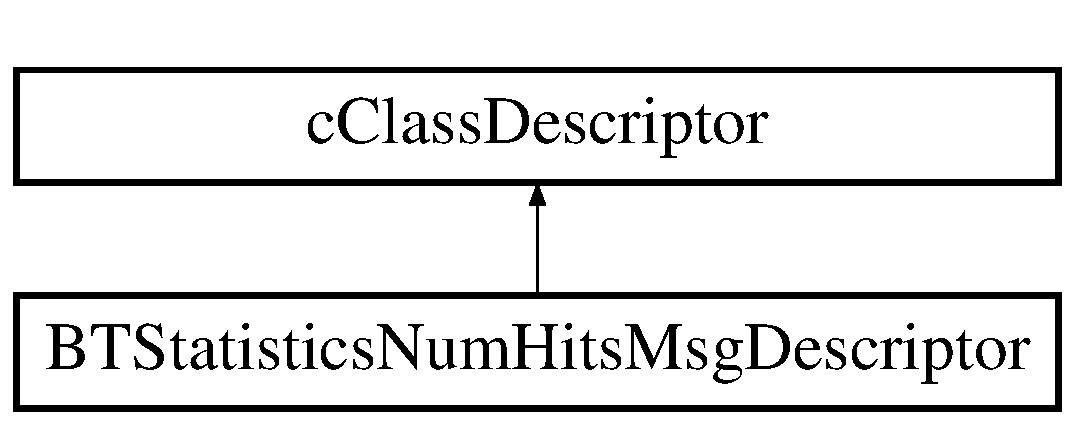
\includegraphics[height=2.000000cm]{classBTStatisticsNumHitsMsgDescriptor}
\end{center}
\end{figure}
\subsection*{Public Member Functions}
\begin{DoxyCompactItemize}
\item 
\hyperlink{classBTStatisticsNumHitsMsgDescriptor_a801f08a77eb9954909e19dc8343cf26c}{B\+T\+Statistics\+Num\+Hits\+Msg\+Descriptor} ()
\item 
virtual \hyperlink{classBTStatisticsNumHitsMsgDescriptor_acd98b9cd8b8706a00321b6f79347b9d6}{$\sim$\+B\+T\+Statistics\+Num\+Hits\+Msg\+Descriptor} ()
\item 
virtual bool \hyperlink{classBTStatisticsNumHitsMsgDescriptor_ad6dadb8660d3bd19273fed98303f9a64}{does\+Support} (c\+Object $\ast$obj) const 
\item 
virtual const char $\ast$ \hyperlink{classBTStatisticsNumHitsMsgDescriptor_a44db1a051fb2565d55c55c2c435cc2a9}{get\+Property} (const char $\ast$propertyname) const 
\item 
virtual int \hyperlink{classBTStatisticsNumHitsMsgDescriptor_a15aeb6bfee67dd9d9838ef087965df4e}{get\+Field\+Count} (void $\ast$object) const 
\item 
virtual const char $\ast$ \hyperlink{classBTStatisticsNumHitsMsgDescriptor_a0ae0e075cd578a55b74c3a2fed17764f}{get\+Field\+Name} (void $\ast$object, int field) const 
\item 
virtual int \hyperlink{classBTStatisticsNumHitsMsgDescriptor_a315fbfbfb1a7ee5380aa2693c04edf0e}{find\+Field} (void $\ast$object, const char $\ast$field\+Name) const 
\item 
virtual unsigned int \hyperlink{classBTStatisticsNumHitsMsgDescriptor_a6a538b7083a27dc960d4a4709e7d909c}{get\+Field\+Type\+Flags} (void $\ast$object, int field) const 
\item 
virtual const char $\ast$ \hyperlink{classBTStatisticsNumHitsMsgDescriptor_aa49fe4d07fd6fd60dd61611fb3858cbc}{get\+Field\+Type\+String} (void $\ast$object, int field) const 
\item 
virtual const char $\ast$ \hyperlink{classBTStatisticsNumHitsMsgDescriptor_af20b093c7bc6664100b9372ba6f81194}{get\+Field\+Property} (void $\ast$object, int field, const char $\ast$propertyname) const 
\item 
virtual int \hyperlink{classBTStatisticsNumHitsMsgDescriptor_a2941241ba1289d68a2e0b38368020d7f}{get\+Array\+Size} (void $\ast$object, int field) const 
\item 
virtual std\+::string \hyperlink{classBTStatisticsNumHitsMsgDescriptor_a5c0638a606f61bcb19cc896d891be9c4}{get\+Field\+As\+String} (void $\ast$object, int field, int i) const 
\item 
virtual bool \hyperlink{classBTStatisticsNumHitsMsgDescriptor_abedb5e8b122e3daf5f6a70212e634bb2}{set\+Field\+As\+String} (void $\ast$object, int field, int i, const char $\ast$value) const 
\item 
virtual const char $\ast$ \hyperlink{classBTStatisticsNumHitsMsgDescriptor_a83119b5997136704c5e6452b28c39559}{get\+Field\+Struct\+Name} (void $\ast$object, int field) const 
\item 
virtual void $\ast$ \hyperlink{classBTStatisticsNumHitsMsgDescriptor_abfe152771ec2882c662d7b65e4e62a95}{get\+Field\+Struct\+Pointer} (void $\ast$object, int field, int i) const 
\end{DoxyCompactItemize}


\subsection{Constructor \& Destructor Documentation}
\hypertarget{classBTStatisticsNumHitsMsgDescriptor_a801f08a77eb9954909e19dc8343cf26c}{}\index{B\+T\+Statistics\+Num\+Hits\+Msg\+Descriptor@{B\+T\+Statistics\+Num\+Hits\+Msg\+Descriptor}!B\+T\+Statistics\+Num\+Hits\+Msg\+Descriptor@{B\+T\+Statistics\+Num\+Hits\+Msg\+Descriptor}}
\index{B\+T\+Statistics\+Num\+Hits\+Msg\+Descriptor@{B\+T\+Statistics\+Num\+Hits\+Msg\+Descriptor}!B\+T\+Statistics\+Num\+Hits\+Msg\+Descriptor@{B\+T\+Statistics\+Num\+Hits\+Msg\+Descriptor}}
\subsubsection[{B\+T\+Statistics\+Num\+Hits\+Msg\+Descriptor()}]{\setlength{\rightskip}{0pt plus 5cm}B\+T\+Statistics\+Num\+Hits\+Msg\+Descriptor\+::\+B\+T\+Statistics\+Num\+Hits\+Msg\+Descriptor (
\begin{DoxyParamCaption}
{}
\end{DoxyParamCaption}
)}\label{classBTStatisticsNumHitsMsgDescriptor_a801f08a77eb9954909e19dc8343cf26c}
\hypertarget{classBTStatisticsNumHitsMsgDescriptor_acd98b9cd8b8706a00321b6f79347b9d6}{}\index{B\+T\+Statistics\+Num\+Hits\+Msg\+Descriptor@{B\+T\+Statistics\+Num\+Hits\+Msg\+Descriptor}!````~B\+T\+Statistics\+Num\+Hits\+Msg\+Descriptor@{$\sim$\+B\+T\+Statistics\+Num\+Hits\+Msg\+Descriptor}}
\index{````~B\+T\+Statistics\+Num\+Hits\+Msg\+Descriptor@{$\sim$\+B\+T\+Statistics\+Num\+Hits\+Msg\+Descriptor}!B\+T\+Statistics\+Num\+Hits\+Msg\+Descriptor@{B\+T\+Statistics\+Num\+Hits\+Msg\+Descriptor}}
\subsubsection[{$\sim$\+B\+T\+Statistics\+Num\+Hits\+Msg\+Descriptor()}]{\setlength{\rightskip}{0pt plus 5cm}B\+T\+Statistics\+Num\+Hits\+Msg\+Descriptor\+::$\sim$\+B\+T\+Statistics\+Num\+Hits\+Msg\+Descriptor (
\begin{DoxyParamCaption}
{}
\end{DoxyParamCaption}
)\hspace{0.3cm}{\ttfamily [virtual]}}\label{classBTStatisticsNumHitsMsgDescriptor_acd98b9cd8b8706a00321b6f79347b9d6}


\subsection{Member Function Documentation}
\hypertarget{classBTStatisticsNumHitsMsgDescriptor_ad6dadb8660d3bd19273fed98303f9a64}{}\index{B\+T\+Statistics\+Num\+Hits\+Msg\+Descriptor@{B\+T\+Statistics\+Num\+Hits\+Msg\+Descriptor}!does\+Support@{does\+Support}}
\index{does\+Support@{does\+Support}!B\+T\+Statistics\+Num\+Hits\+Msg\+Descriptor@{B\+T\+Statistics\+Num\+Hits\+Msg\+Descriptor}}
\subsubsection[{does\+Support(c\+Object $\ast$obj) const }]{\setlength{\rightskip}{0pt plus 5cm}bool B\+T\+Statistics\+Num\+Hits\+Msg\+Descriptor\+::does\+Support (
\begin{DoxyParamCaption}
\item[{c\+Object $\ast$}]{obj}
\end{DoxyParamCaption}
) const\hspace{0.3cm}{\ttfamily [virtual]}}\label{classBTStatisticsNumHitsMsgDescriptor_ad6dadb8660d3bd19273fed98303f9a64}
\hypertarget{classBTStatisticsNumHitsMsgDescriptor_a315fbfbfb1a7ee5380aa2693c04edf0e}{}\index{B\+T\+Statistics\+Num\+Hits\+Msg\+Descriptor@{B\+T\+Statistics\+Num\+Hits\+Msg\+Descriptor}!find\+Field@{find\+Field}}
\index{find\+Field@{find\+Field}!B\+T\+Statistics\+Num\+Hits\+Msg\+Descriptor@{B\+T\+Statistics\+Num\+Hits\+Msg\+Descriptor}}
\subsubsection[{find\+Field(void $\ast$object, const char $\ast$field\+Name) const }]{\setlength{\rightskip}{0pt plus 5cm}int B\+T\+Statistics\+Num\+Hits\+Msg\+Descriptor\+::find\+Field (
\begin{DoxyParamCaption}
\item[{void $\ast$}]{object, }
\item[{const char $\ast$}]{field\+Name}
\end{DoxyParamCaption}
) const\hspace{0.3cm}{\ttfamily [virtual]}}\label{classBTStatisticsNumHitsMsgDescriptor_a315fbfbfb1a7ee5380aa2693c04edf0e}
\hypertarget{classBTStatisticsNumHitsMsgDescriptor_a2941241ba1289d68a2e0b38368020d7f}{}\index{B\+T\+Statistics\+Num\+Hits\+Msg\+Descriptor@{B\+T\+Statistics\+Num\+Hits\+Msg\+Descriptor}!get\+Array\+Size@{get\+Array\+Size}}
\index{get\+Array\+Size@{get\+Array\+Size}!B\+T\+Statistics\+Num\+Hits\+Msg\+Descriptor@{B\+T\+Statistics\+Num\+Hits\+Msg\+Descriptor}}
\subsubsection[{get\+Array\+Size(void $\ast$object, int field) const }]{\setlength{\rightskip}{0pt plus 5cm}int B\+T\+Statistics\+Num\+Hits\+Msg\+Descriptor\+::get\+Array\+Size (
\begin{DoxyParamCaption}
\item[{void $\ast$}]{object, }
\item[{int}]{field}
\end{DoxyParamCaption}
) const\hspace{0.3cm}{\ttfamily [virtual]}}\label{classBTStatisticsNumHitsMsgDescriptor_a2941241ba1289d68a2e0b38368020d7f}
\hypertarget{classBTStatisticsNumHitsMsgDescriptor_a5c0638a606f61bcb19cc896d891be9c4}{}\index{B\+T\+Statistics\+Num\+Hits\+Msg\+Descriptor@{B\+T\+Statistics\+Num\+Hits\+Msg\+Descriptor}!get\+Field\+As\+String@{get\+Field\+As\+String}}
\index{get\+Field\+As\+String@{get\+Field\+As\+String}!B\+T\+Statistics\+Num\+Hits\+Msg\+Descriptor@{B\+T\+Statistics\+Num\+Hits\+Msg\+Descriptor}}
\subsubsection[{get\+Field\+As\+String(void $\ast$object, int field, int i) const }]{\setlength{\rightskip}{0pt plus 5cm}std\+::string B\+T\+Statistics\+Num\+Hits\+Msg\+Descriptor\+::get\+Field\+As\+String (
\begin{DoxyParamCaption}
\item[{void $\ast$}]{object, }
\item[{int}]{field, }
\item[{int}]{i}
\end{DoxyParamCaption}
) const\hspace{0.3cm}{\ttfamily [virtual]}}\label{classBTStatisticsNumHitsMsgDescriptor_a5c0638a606f61bcb19cc896d891be9c4}
\hypertarget{classBTStatisticsNumHitsMsgDescriptor_a15aeb6bfee67dd9d9838ef087965df4e}{}\index{B\+T\+Statistics\+Num\+Hits\+Msg\+Descriptor@{B\+T\+Statistics\+Num\+Hits\+Msg\+Descriptor}!get\+Field\+Count@{get\+Field\+Count}}
\index{get\+Field\+Count@{get\+Field\+Count}!B\+T\+Statistics\+Num\+Hits\+Msg\+Descriptor@{B\+T\+Statistics\+Num\+Hits\+Msg\+Descriptor}}
\subsubsection[{get\+Field\+Count(void $\ast$object) const }]{\setlength{\rightskip}{0pt plus 5cm}int B\+T\+Statistics\+Num\+Hits\+Msg\+Descriptor\+::get\+Field\+Count (
\begin{DoxyParamCaption}
\item[{void $\ast$}]{object}
\end{DoxyParamCaption}
) const\hspace{0.3cm}{\ttfamily [virtual]}}\label{classBTStatisticsNumHitsMsgDescriptor_a15aeb6bfee67dd9d9838ef087965df4e}
\hypertarget{classBTStatisticsNumHitsMsgDescriptor_a0ae0e075cd578a55b74c3a2fed17764f}{}\index{B\+T\+Statistics\+Num\+Hits\+Msg\+Descriptor@{B\+T\+Statistics\+Num\+Hits\+Msg\+Descriptor}!get\+Field\+Name@{get\+Field\+Name}}
\index{get\+Field\+Name@{get\+Field\+Name}!B\+T\+Statistics\+Num\+Hits\+Msg\+Descriptor@{B\+T\+Statistics\+Num\+Hits\+Msg\+Descriptor}}
\subsubsection[{get\+Field\+Name(void $\ast$object, int field) const }]{\setlength{\rightskip}{0pt plus 5cm}const char $\ast$ B\+T\+Statistics\+Num\+Hits\+Msg\+Descriptor\+::get\+Field\+Name (
\begin{DoxyParamCaption}
\item[{void $\ast$}]{object, }
\item[{int}]{field}
\end{DoxyParamCaption}
) const\hspace{0.3cm}{\ttfamily [virtual]}}\label{classBTStatisticsNumHitsMsgDescriptor_a0ae0e075cd578a55b74c3a2fed17764f}
\hypertarget{classBTStatisticsNumHitsMsgDescriptor_af20b093c7bc6664100b9372ba6f81194}{}\index{B\+T\+Statistics\+Num\+Hits\+Msg\+Descriptor@{B\+T\+Statistics\+Num\+Hits\+Msg\+Descriptor}!get\+Field\+Property@{get\+Field\+Property}}
\index{get\+Field\+Property@{get\+Field\+Property}!B\+T\+Statistics\+Num\+Hits\+Msg\+Descriptor@{B\+T\+Statistics\+Num\+Hits\+Msg\+Descriptor}}
\subsubsection[{get\+Field\+Property(void $\ast$object, int field, const char $\ast$propertyname) const }]{\setlength{\rightskip}{0pt plus 5cm}const char $\ast$ B\+T\+Statistics\+Num\+Hits\+Msg\+Descriptor\+::get\+Field\+Property (
\begin{DoxyParamCaption}
\item[{void $\ast$}]{object, }
\item[{int}]{field, }
\item[{const char $\ast$}]{propertyname}
\end{DoxyParamCaption}
) const\hspace{0.3cm}{\ttfamily [virtual]}}\label{classBTStatisticsNumHitsMsgDescriptor_af20b093c7bc6664100b9372ba6f81194}
\hypertarget{classBTStatisticsNumHitsMsgDescriptor_a83119b5997136704c5e6452b28c39559}{}\index{B\+T\+Statistics\+Num\+Hits\+Msg\+Descriptor@{B\+T\+Statistics\+Num\+Hits\+Msg\+Descriptor}!get\+Field\+Struct\+Name@{get\+Field\+Struct\+Name}}
\index{get\+Field\+Struct\+Name@{get\+Field\+Struct\+Name}!B\+T\+Statistics\+Num\+Hits\+Msg\+Descriptor@{B\+T\+Statistics\+Num\+Hits\+Msg\+Descriptor}}
\subsubsection[{get\+Field\+Struct\+Name(void $\ast$object, int field) const }]{\setlength{\rightskip}{0pt plus 5cm}const char $\ast$ B\+T\+Statistics\+Num\+Hits\+Msg\+Descriptor\+::get\+Field\+Struct\+Name (
\begin{DoxyParamCaption}
\item[{void $\ast$}]{object, }
\item[{int}]{field}
\end{DoxyParamCaption}
) const\hspace{0.3cm}{\ttfamily [virtual]}}\label{classBTStatisticsNumHitsMsgDescriptor_a83119b5997136704c5e6452b28c39559}
\hypertarget{classBTStatisticsNumHitsMsgDescriptor_abfe152771ec2882c662d7b65e4e62a95}{}\index{B\+T\+Statistics\+Num\+Hits\+Msg\+Descriptor@{B\+T\+Statistics\+Num\+Hits\+Msg\+Descriptor}!get\+Field\+Struct\+Pointer@{get\+Field\+Struct\+Pointer}}
\index{get\+Field\+Struct\+Pointer@{get\+Field\+Struct\+Pointer}!B\+T\+Statistics\+Num\+Hits\+Msg\+Descriptor@{B\+T\+Statistics\+Num\+Hits\+Msg\+Descriptor}}
\subsubsection[{get\+Field\+Struct\+Pointer(void $\ast$object, int field, int i) const }]{\setlength{\rightskip}{0pt plus 5cm}void $\ast$ B\+T\+Statistics\+Num\+Hits\+Msg\+Descriptor\+::get\+Field\+Struct\+Pointer (
\begin{DoxyParamCaption}
\item[{void $\ast$}]{object, }
\item[{int}]{field, }
\item[{int}]{i}
\end{DoxyParamCaption}
) const\hspace{0.3cm}{\ttfamily [virtual]}}\label{classBTStatisticsNumHitsMsgDescriptor_abfe152771ec2882c662d7b65e4e62a95}
\hypertarget{classBTStatisticsNumHitsMsgDescriptor_a6a538b7083a27dc960d4a4709e7d909c}{}\index{B\+T\+Statistics\+Num\+Hits\+Msg\+Descriptor@{B\+T\+Statistics\+Num\+Hits\+Msg\+Descriptor}!get\+Field\+Type\+Flags@{get\+Field\+Type\+Flags}}
\index{get\+Field\+Type\+Flags@{get\+Field\+Type\+Flags}!B\+T\+Statistics\+Num\+Hits\+Msg\+Descriptor@{B\+T\+Statistics\+Num\+Hits\+Msg\+Descriptor}}
\subsubsection[{get\+Field\+Type\+Flags(void $\ast$object, int field) const }]{\setlength{\rightskip}{0pt plus 5cm}unsigned int B\+T\+Statistics\+Num\+Hits\+Msg\+Descriptor\+::get\+Field\+Type\+Flags (
\begin{DoxyParamCaption}
\item[{void $\ast$}]{object, }
\item[{int}]{field}
\end{DoxyParamCaption}
) const\hspace{0.3cm}{\ttfamily [virtual]}}\label{classBTStatisticsNumHitsMsgDescriptor_a6a538b7083a27dc960d4a4709e7d909c}
\hypertarget{classBTStatisticsNumHitsMsgDescriptor_aa49fe4d07fd6fd60dd61611fb3858cbc}{}\index{B\+T\+Statistics\+Num\+Hits\+Msg\+Descriptor@{B\+T\+Statistics\+Num\+Hits\+Msg\+Descriptor}!get\+Field\+Type\+String@{get\+Field\+Type\+String}}
\index{get\+Field\+Type\+String@{get\+Field\+Type\+String}!B\+T\+Statistics\+Num\+Hits\+Msg\+Descriptor@{B\+T\+Statistics\+Num\+Hits\+Msg\+Descriptor}}
\subsubsection[{get\+Field\+Type\+String(void $\ast$object, int field) const }]{\setlength{\rightskip}{0pt plus 5cm}const char $\ast$ B\+T\+Statistics\+Num\+Hits\+Msg\+Descriptor\+::get\+Field\+Type\+String (
\begin{DoxyParamCaption}
\item[{void $\ast$}]{object, }
\item[{int}]{field}
\end{DoxyParamCaption}
) const\hspace{0.3cm}{\ttfamily [virtual]}}\label{classBTStatisticsNumHitsMsgDescriptor_aa49fe4d07fd6fd60dd61611fb3858cbc}
\hypertarget{classBTStatisticsNumHitsMsgDescriptor_a44db1a051fb2565d55c55c2c435cc2a9}{}\index{B\+T\+Statistics\+Num\+Hits\+Msg\+Descriptor@{B\+T\+Statistics\+Num\+Hits\+Msg\+Descriptor}!get\+Property@{get\+Property}}
\index{get\+Property@{get\+Property}!B\+T\+Statistics\+Num\+Hits\+Msg\+Descriptor@{B\+T\+Statistics\+Num\+Hits\+Msg\+Descriptor}}
\subsubsection[{get\+Property(const char $\ast$propertyname) const }]{\setlength{\rightskip}{0pt plus 5cm}const char $\ast$ B\+T\+Statistics\+Num\+Hits\+Msg\+Descriptor\+::get\+Property (
\begin{DoxyParamCaption}
\item[{const char $\ast$}]{propertyname}
\end{DoxyParamCaption}
) const\hspace{0.3cm}{\ttfamily [virtual]}}\label{classBTStatisticsNumHitsMsgDescriptor_a44db1a051fb2565d55c55c2c435cc2a9}
\hypertarget{classBTStatisticsNumHitsMsgDescriptor_abedb5e8b122e3daf5f6a70212e634bb2}{}\index{B\+T\+Statistics\+Num\+Hits\+Msg\+Descriptor@{B\+T\+Statistics\+Num\+Hits\+Msg\+Descriptor}!set\+Field\+As\+String@{set\+Field\+As\+String}}
\index{set\+Field\+As\+String@{set\+Field\+As\+String}!B\+T\+Statistics\+Num\+Hits\+Msg\+Descriptor@{B\+T\+Statistics\+Num\+Hits\+Msg\+Descriptor}}
\subsubsection[{set\+Field\+As\+String(void $\ast$object, int field, int i, const char $\ast$value) const }]{\setlength{\rightskip}{0pt plus 5cm}bool B\+T\+Statistics\+Num\+Hits\+Msg\+Descriptor\+::set\+Field\+As\+String (
\begin{DoxyParamCaption}
\item[{void $\ast$}]{object, }
\item[{int}]{field, }
\item[{int}]{i, }
\item[{const char $\ast$}]{value}
\end{DoxyParamCaption}
) const\hspace{0.3cm}{\ttfamily [virtual]}}\label{classBTStatisticsNumHitsMsgDescriptor_abedb5e8b122e3daf5f6a70212e634bb2}


The documentation for this class was generated from the following file\+:\begin{DoxyCompactItemize}
\item 
\hyperlink{BTStatisticsMsg__m_8cc}{B\+T\+Statistics\+Msg\+\_\+m.\+cc}\end{DoxyCompactItemize}

\hypertarget{classBTStatisticsNumMissesMsg}{}\section{B\+T\+Statistics\+Num\+Misses\+Msg Class Reference}
\label{classBTStatisticsNumMissesMsg}\index{B\+T\+Statistics\+Num\+Misses\+Msg@{B\+T\+Statistics\+Num\+Misses\+Msg}}


{\ttfamily \#include $<$B\+T\+Statistics\+Msg\+\_\+m.\+h$>$}

Inheritance diagram for B\+T\+Statistics\+Num\+Misses\+Msg\+:\begin{figure}[H]
\begin{center}
\leavevmode
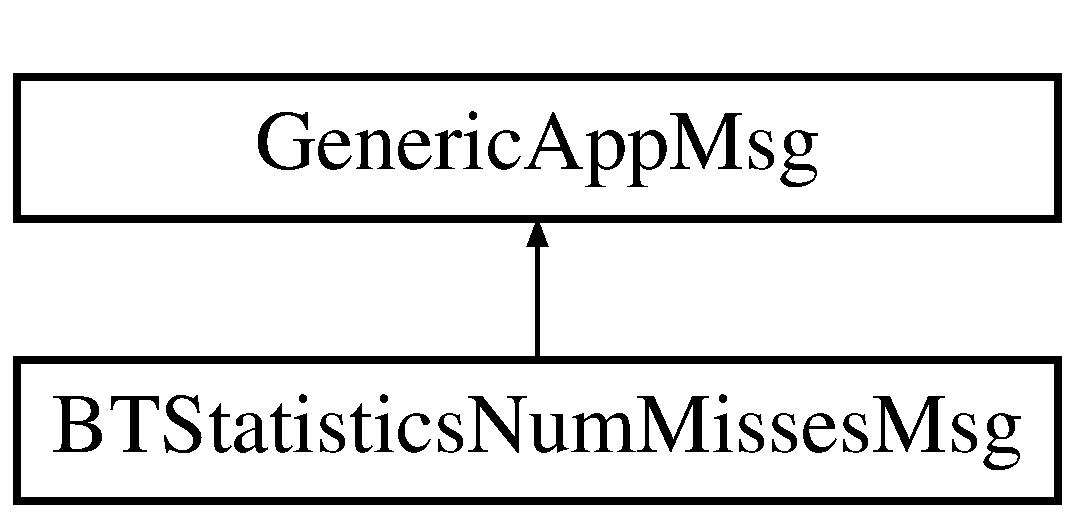
\includegraphics[height=2.000000cm]{classBTStatisticsNumMissesMsg}
\end{center}
\end{figure}
\subsection*{Public Member Functions}
\begin{DoxyCompactItemize}
\item 
\hyperlink{classBTStatisticsNumMissesMsg_a12062190375e684b1ab12e51b3b11e6d}{B\+T\+Statistics\+Num\+Misses\+Msg} (const char $\ast$name=N\+U\+L\+L, int kind=0)
\item 
\hyperlink{classBTStatisticsNumMissesMsg_ab731ecc85c292a7d74d99bf09c099e57}{B\+T\+Statistics\+Num\+Misses\+Msg} (const \hyperlink{classBTStatisticsNumMissesMsg}{B\+T\+Statistics\+Num\+Misses\+Msg} \&other)
\item 
virtual \hyperlink{classBTStatisticsNumMissesMsg_a07705f4e854c08cca570365556993408}{$\sim$\+B\+T\+Statistics\+Num\+Misses\+Msg} ()
\item 
\hyperlink{classBTStatisticsNumMissesMsg}{B\+T\+Statistics\+Num\+Misses\+Msg} \& \hyperlink{classBTStatisticsNumMissesMsg_a4975eb2d2cc3f64083f4a643c236fcff}{operator=} (const \hyperlink{classBTStatisticsNumMissesMsg}{B\+T\+Statistics\+Num\+Misses\+Msg} \&other)
\item 
virtual \hyperlink{classBTStatisticsNumMissesMsg}{B\+T\+Statistics\+Num\+Misses\+Msg} $\ast$ \hyperlink{classBTStatisticsNumMissesMsg_ac9bf69db530be787cb6b13063927f8e1}{dup} () const 
\item 
virtual void \hyperlink{classBTStatisticsNumMissesMsg_af0ede08af67692ee012ee06f076a5a67}{parsim\+Pack} (c\+Comm\+Buffer $\ast$b)
\item 
virtual void \hyperlink{classBTStatisticsNumMissesMsg_a80c048371a7e616236d8f3118d59e6b3}{parsim\+Unpack} (c\+Comm\+Buffer $\ast$b)
\item 
virtual double \hyperlink{classBTStatisticsNumMissesMsg_a92411392b465eb6262f7ca3cd17b9195}{num\+Misses} () const 
\item 
virtual void \hyperlink{classBTStatisticsNumMissesMsg_ab89ff20783a4bed86f5eb21e58ae09b6}{set\+Num\+Misses} (double \hyperlink{classBTStatisticsNumMissesMsg_a28bbdae0b44bd313c2377e841097b5b4}{num\+Misses\+\_\+var})
\end{DoxyCompactItemize}
\subsection*{Protected Member Functions}
\begin{DoxyCompactItemize}
\item 
bool \hyperlink{classBTStatisticsNumMissesMsg_acced5f9552f3768cd03717ac574190b8}{operator==} (const \hyperlink{classBTStatisticsNumMissesMsg}{B\+T\+Statistics\+Num\+Misses\+Msg} \&)
\end{DoxyCompactItemize}
\subsection*{Protected Attributes}
\begin{DoxyCompactItemize}
\item 
double \hyperlink{classBTStatisticsNumMissesMsg_a28bbdae0b44bd313c2377e841097b5b4}{num\+Misses\+\_\+var}
\end{DoxyCompactItemize}


\subsection{Detailed Description}
Class generated from {\ttfamily applications/x\+Bit\+Torrent/\+B\+T\+Statistics\+Msg.\+msg} by opp\+\_\+msgc. 
\begin{DoxyPre}
message \hyperlink{classBTStatisticsNumMissesMsg}{BTStatisticsNumMissesMsg} extends GenericAppMsg
\{
     (true);\end{DoxyPre}



\begin{DoxyPre}    double numMisses;
\}
\end{DoxyPre}
 

\subsection{Constructor \& Destructor Documentation}
\hypertarget{classBTStatisticsNumMissesMsg_a12062190375e684b1ab12e51b3b11e6d}{}\index{B\+T\+Statistics\+Num\+Misses\+Msg@{B\+T\+Statistics\+Num\+Misses\+Msg}!B\+T\+Statistics\+Num\+Misses\+Msg@{B\+T\+Statistics\+Num\+Misses\+Msg}}
\index{B\+T\+Statistics\+Num\+Misses\+Msg@{B\+T\+Statistics\+Num\+Misses\+Msg}!B\+T\+Statistics\+Num\+Misses\+Msg@{B\+T\+Statistics\+Num\+Misses\+Msg}}
\subsubsection[{B\+T\+Statistics\+Num\+Misses\+Msg(const char $\ast$name=\+N\+U\+L\+L, int kind=0)}]{\setlength{\rightskip}{0pt plus 5cm}B\+T\+Statistics\+Num\+Misses\+Msg\+::\+B\+T\+Statistics\+Num\+Misses\+Msg (
\begin{DoxyParamCaption}
\item[{const char $\ast$}]{name = {\ttfamily NULL}, }
\item[{int}]{kind = {\ttfamily 0}}
\end{DoxyParamCaption}
)}\label{classBTStatisticsNumMissesMsg_a12062190375e684b1ab12e51b3b11e6d}
\hypertarget{classBTStatisticsNumMissesMsg_ab731ecc85c292a7d74d99bf09c099e57}{}\index{B\+T\+Statistics\+Num\+Misses\+Msg@{B\+T\+Statistics\+Num\+Misses\+Msg}!B\+T\+Statistics\+Num\+Misses\+Msg@{B\+T\+Statistics\+Num\+Misses\+Msg}}
\index{B\+T\+Statistics\+Num\+Misses\+Msg@{B\+T\+Statistics\+Num\+Misses\+Msg}!B\+T\+Statistics\+Num\+Misses\+Msg@{B\+T\+Statistics\+Num\+Misses\+Msg}}
\subsubsection[{B\+T\+Statistics\+Num\+Misses\+Msg(const B\+T\+Statistics\+Num\+Misses\+Msg \&other)}]{\setlength{\rightskip}{0pt plus 5cm}B\+T\+Statistics\+Num\+Misses\+Msg\+::\+B\+T\+Statistics\+Num\+Misses\+Msg (
\begin{DoxyParamCaption}
\item[{const {\bf B\+T\+Statistics\+Num\+Misses\+Msg} \&}]{other}
\end{DoxyParamCaption}
)}\label{classBTStatisticsNumMissesMsg_ab731ecc85c292a7d74d99bf09c099e57}
\hypertarget{classBTStatisticsNumMissesMsg_a07705f4e854c08cca570365556993408}{}\index{B\+T\+Statistics\+Num\+Misses\+Msg@{B\+T\+Statistics\+Num\+Misses\+Msg}!````~B\+T\+Statistics\+Num\+Misses\+Msg@{$\sim$\+B\+T\+Statistics\+Num\+Misses\+Msg}}
\index{````~B\+T\+Statistics\+Num\+Misses\+Msg@{$\sim$\+B\+T\+Statistics\+Num\+Misses\+Msg}!B\+T\+Statistics\+Num\+Misses\+Msg@{B\+T\+Statistics\+Num\+Misses\+Msg}}
\subsubsection[{$\sim$\+B\+T\+Statistics\+Num\+Misses\+Msg()}]{\setlength{\rightskip}{0pt plus 5cm}B\+T\+Statistics\+Num\+Misses\+Msg\+::$\sim$\+B\+T\+Statistics\+Num\+Misses\+Msg (
\begin{DoxyParamCaption}
{}
\end{DoxyParamCaption}
)\hspace{0.3cm}{\ttfamily [virtual]}}\label{classBTStatisticsNumMissesMsg_a07705f4e854c08cca570365556993408}


\subsection{Member Function Documentation}
\hypertarget{classBTStatisticsNumMissesMsg_ac9bf69db530be787cb6b13063927f8e1}{}\index{B\+T\+Statistics\+Num\+Misses\+Msg@{B\+T\+Statistics\+Num\+Misses\+Msg}!dup@{dup}}
\index{dup@{dup}!B\+T\+Statistics\+Num\+Misses\+Msg@{B\+T\+Statistics\+Num\+Misses\+Msg}}
\subsubsection[{dup() const }]{\setlength{\rightskip}{0pt plus 5cm}virtual {\bf B\+T\+Statistics\+Num\+Misses\+Msg}$\ast$ B\+T\+Statistics\+Num\+Misses\+Msg\+::dup (
\begin{DoxyParamCaption}
{}
\end{DoxyParamCaption}
) const\hspace{0.3cm}{\ttfamily [inline]}, {\ttfamily [virtual]}}\label{classBTStatisticsNumMissesMsg_ac9bf69db530be787cb6b13063927f8e1}
\hypertarget{classBTStatisticsNumMissesMsg_a92411392b465eb6262f7ca3cd17b9195}{}\index{B\+T\+Statistics\+Num\+Misses\+Msg@{B\+T\+Statistics\+Num\+Misses\+Msg}!num\+Misses@{num\+Misses}}
\index{num\+Misses@{num\+Misses}!B\+T\+Statistics\+Num\+Misses\+Msg@{B\+T\+Statistics\+Num\+Misses\+Msg}}
\subsubsection[{num\+Misses() const }]{\setlength{\rightskip}{0pt plus 5cm}double B\+T\+Statistics\+Num\+Misses\+Msg\+::num\+Misses (
\begin{DoxyParamCaption}
{}
\end{DoxyParamCaption}
) const\hspace{0.3cm}{\ttfamily [virtual]}}\label{classBTStatisticsNumMissesMsg_a92411392b465eb6262f7ca3cd17b9195}
\hypertarget{classBTStatisticsNumMissesMsg_a4975eb2d2cc3f64083f4a643c236fcff}{}\index{B\+T\+Statistics\+Num\+Misses\+Msg@{B\+T\+Statistics\+Num\+Misses\+Msg}!operator=@{operator=}}
\index{operator=@{operator=}!B\+T\+Statistics\+Num\+Misses\+Msg@{B\+T\+Statistics\+Num\+Misses\+Msg}}
\subsubsection[{operator=(const B\+T\+Statistics\+Num\+Misses\+Msg \&other)}]{\setlength{\rightskip}{0pt plus 5cm}{\bf B\+T\+Statistics\+Num\+Misses\+Msg} \& B\+T\+Statistics\+Num\+Misses\+Msg\+::operator= (
\begin{DoxyParamCaption}
\item[{const {\bf B\+T\+Statistics\+Num\+Misses\+Msg} \&}]{other}
\end{DoxyParamCaption}
)}\label{classBTStatisticsNumMissesMsg_a4975eb2d2cc3f64083f4a643c236fcff}
\hypertarget{classBTStatisticsNumMissesMsg_acced5f9552f3768cd03717ac574190b8}{}\index{B\+T\+Statistics\+Num\+Misses\+Msg@{B\+T\+Statistics\+Num\+Misses\+Msg}!operator==@{operator==}}
\index{operator==@{operator==}!B\+T\+Statistics\+Num\+Misses\+Msg@{B\+T\+Statistics\+Num\+Misses\+Msg}}
\subsubsection[{operator==(const B\+T\+Statistics\+Num\+Misses\+Msg \&)}]{\setlength{\rightskip}{0pt plus 5cm}bool B\+T\+Statistics\+Num\+Misses\+Msg\+::operator== (
\begin{DoxyParamCaption}
\item[{const {\bf B\+T\+Statistics\+Num\+Misses\+Msg} \&}]{}
\end{DoxyParamCaption}
)\hspace{0.3cm}{\ttfamily [protected]}}\label{classBTStatisticsNumMissesMsg_acced5f9552f3768cd03717ac574190b8}
\hypertarget{classBTStatisticsNumMissesMsg_af0ede08af67692ee012ee06f076a5a67}{}\index{B\+T\+Statistics\+Num\+Misses\+Msg@{B\+T\+Statistics\+Num\+Misses\+Msg}!parsim\+Pack@{parsim\+Pack}}
\index{parsim\+Pack@{parsim\+Pack}!B\+T\+Statistics\+Num\+Misses\+Msg@{B\+T\+Statistics\+Num\+Misses\+Msg}}
\subsubsection[{parsim\+Pack(c\+Comm\+Buffer $\ast$b)}]{\setlength{\rightskip}{0pt plus 5cm}void B\+T\+Statistics\+Num\+Misses\+Msg\+::parsim\+Pack (
\begin{DoxyParamCaption}
\item[{c\+Comm\+Buffer $\ast$}]{b}
\end{DoxyParamCaption}
)\hspace{0.3cm}{\ttfamily [virtual]}}\label{classBTStatisticsNumMissesMsg_af0ede08af67692ee012ee06f076a5a67}
\hypertarget{classBTStatisticsNumMissesMsg_a80c048371a7e616236d8f3118d59e6b3}{}\index{B\+T\+Statistics\+Num\+Misses\+Msg@{B\+T\+Statistics\+Num\+Misses\+Msg}!parsim\+Unpack@{parsim\+Unpack}}
\index{parsim\+Unpack@{parsim\+Unpack}!B\+T\+Statistics\+Num\+Misses\+Msg@{B\+T\+Statistics\+Num\+Misses\+Msg}}
\subsubsection[{parsim\+Unpack(c\+Comm\+Buffer $\ast$b)}]{\setlength{\rightskip}{0pt plus 5cm}void B\+T\+Statistics\+Num\+Misses\+Msg\+::parsim\+Unpack (
\begin{DoxyParamCaption}
\item[{c\+Comm\+Buffer $\ast$}]{b}
\end{DoxyParamCaption}
)\hspace{0.3cm}{\ttfamily [virtual]}}\label{classBTStatisticsNumMissesMsg_a80c048371a7e616236d8f3118d59e6b3}
\hypertarget{classBTStatisticsNumMissesMsg_ab89ff20783a4bed86f5eb21e58ae09b6}{}\index{B\+T\+Statistics\+Num\+Misses\+Msg@{B\+T\+Statistics\+Num\+Misses\+Msg}!set\+Num\+Misses@{set\+Num\+Misses}}
\index{set\+Num\+Misses@{set\+Num\+Misses}!B\+T\+Statistics\+Num\+Misses\+Msg@{B\+T\+Statistics\+Num\+Misses\+Msg}}
\subsubsection[{set\+Num\+Misses(double num\+Misses\+\_\+var)}]{\setlength{\rightskip}{0pt plus 5cm}void B\+T\+Statistics\+Num\+Misses\+Msg\+::set\+Num\+Misses (
\begin{DoxyParamCaption}
\item[{double}]{num\+Misses\+\_\+var}
\end{DoxyParamCaption}
)\hspace{0.3cm}{\ttfamily [virtual]}}\label{classBTStatisticsNumMissesMsg_ab89ff20783a4bed86f5eb21e58ae09b6}


\subsection{Member Data Documentation}
\hypertarget{classBTStatisticsNumMissesMsg_a28bbdae0b44bd313c2377e841097b5b4}{}\index{B\+T\+Statistics\+Num\+Misses\+Msg@{B\+T\+Statistics\+Num\+Misses\+Msg}!num\+Misses\+\_\+var@{num\+Misses\+\_\+var}}
\index{num\+Misses\+\_\+var@{num\+Misses\+\_\+var}!B\+T\+Statistics\+Num\+Misses\+Msg@{B\+T\+Statistics\+Num\+Misses\+Msg}}
\subsubsection[{num\+Misses\+\_\+var}]{\setlength{\rightskip}{0pt plus 5cm}double B\+T\+Statistics\+Num\+Misses\+Msg\+::num\+Misses\+\_\+var\hspace{0.3cm}{\ttfamily [protected]}}\label{classBTStatisticsNumMissesMsg_a28bbdae0b44bd313c2377e841097b5b4}


The documentation for this class was generated from the following files\+:\begin{DoxyCompactItemize}
\item 
\hyperlink{BTStatisticsMsg__m_8h}{B\+T\+Statistics\+Msg\+\_\+m.\+h}\item 
\hyperlink{BTStatisticsMsg__m_8cc}{B\+T\+Statistics\+Msg\+\_\+m.\+cc}\end{DoxyCompactItemize}

\hypertarget{classBTStatisticsNumMissesMsgDescriptor}{}\section{B\+T\+Statistics\+Num\+Misses\+Msg\+Descriptor Class Reference}
\label{classBTStatisticsNumMissesMsgDescriptor}\index{B\+T\+Statistics\+Num\+Misses\+Msg\+Descriptor@{B\+T\+Statistics\+Num\+Misses\+Msg\+Descriptor}}
Inheritance diagram for B\+T\+Statistics\+Num\+Misses\+Msg\+Descriptor\+:\begin{figure}[H]
\begin{center}
\leavevmode
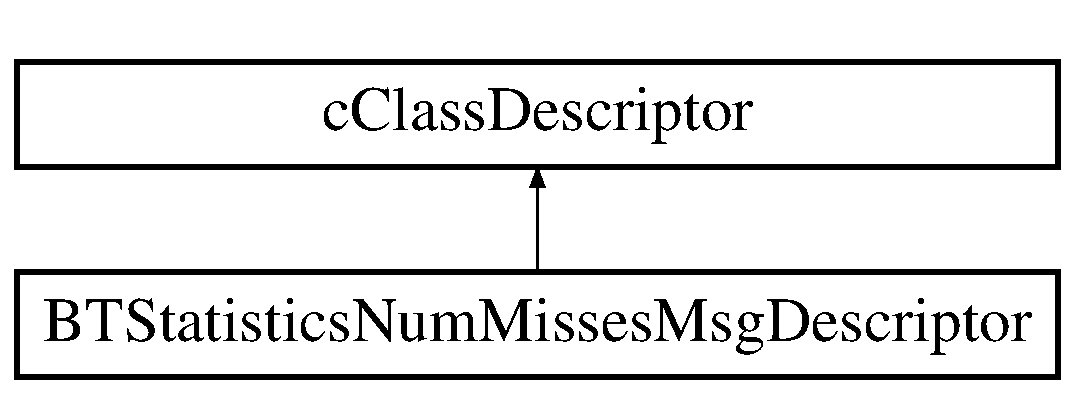
\includegraphics[height=2.000000cm]{classBTStatisticsNumMissesMsgDescriptor}
\end{center}
\end{figure}
\subsection*{Public Member Functions}
\begin{DoxyCompactItemize}
\item 
\hyperlink{classBTStatisticsNumMissesMsgDescriptor_aaa972febe245f79b6e788cd7d0b5fdf2}{B\+T\+Statistics\+Num\+Misses\+Msg\+Descriptor} ()
\item 
virtual \hyperlink{classBTStatisticsNumMissesMsgDescriptor_a92f7ab314eee897bc0e75ddadc19d467}{$\sim$\+B\+T\+Statistics\+Num\+Misses\+Msg\+Descriptor} ()
\item 
virtual bool \hyperlink{classBTStatisticsNumMissesMsgDescriptor_ac8a7c65e6a0f79482dcd0de7085577f5}{does\+Support} (c\+Object $\ast$obj) const 
\item 
virtual const char $\ast$ \hyperlink{classBTStatisticsNumMissesMsgDescriptor_afa165de4d7c72b01217538f5874960ef}{get\+Property} (const char $\ast$propertyname) const 
\item 
virtual int \hyperlink{classBTStatisticsNumMissesMsgDescriptor_ae4ff1f44f80e3368327a600616fc8376}{get\+Field\+Count} (void $\ast$object) const 
\item 
virtual const char $\ast$ \hyperlink{classBTStatisticsNumMissesMsgDescriptor_a0f7c21671d15111f2a0767a2539d20be}{get\+Field\+Name} (void $\ast$object, int field) const 
\item 
virtual int \hyperlink{classBTStatisticsNumMissesMsgDescriptor_a339cda8138d4faad0dad36ce6a6e9dd4}{find\+Field} (void $\ast$object, const char $\ast$field\+Name) const 
\item 
virtual unsigned int \hyperlink{classBTStatisticsNumMissesMsgDescriptor_a138c2af9086b5c94bdd853f7556760ac}{get\+Field\+Type\+Flags} (void $\ast$object, int field) const 
\item 
virtual const char $\ast$ \hyperlink{classBTStatisticsNumMissesMsgDescriptor_af25a045e9900358a0c1cb7f4e8ad2ee9}{get\+Field\+Type\+String} (void $\ast$object, int field) const 
\item 
virtual const char $\ast$ \hyperlink{classBTStatisticsNumMissesMsgDescriptor_a7ff6df5fa866210f4b0ef04794f896be}{get\+Field\+Property} (void $\ast$object, int field, const char $\ast$propertyname) const 
\item 
virtual int \hyperlink{classBTStatisticsNumMissesMsgDescriptor_ac6513df57f60b2ed271dbe935a5cc31b}{get\+Array\+Size} (void $\ast$object, int field) const 
\item 
virtual std\+::string \hyperlink{classBTStatisticsNumMissesMsgDescriptor_a6e7eb1f090778f091ef1925f011d9405}{get\+Field\+As\+String} (void $\ast$object, int field, int i) const 
\item 
virtual bool \hyperlink{classBTStatisticsNumMissesMsgDescriptor_a6469e5254bd1cb026bc198192e3ad370}{set\+Field\+As\+String} (void $\ast$object, int field, int i, const char $\ast$value) const 
\item 
virtual const char $\ast$ \hyperlink{classBTStatisticsNumMissesMsgDescriptor_aaad08633eb0a2165f7f1ff60ca2ee38e}{get\+Field\+Struct\+Name} (void $\ast$object, int field) const 
\item 
virtual void $\ast$ \hyperlink{classBTStatisticsNumMissesMsgDescriptor_a306bb361e95928478db0e47151511274}{get\+Field\+Struct\+Pointer} (void $\ast$object, int field, int i) const 
\end{DoxyCompactItemize}


\subsection{Constructor \& Destructor Documentation}
\hypertarget{classBTStatisticsNumMissesMsgDescriptor_aaa972febe245f79b6e788cd7d0b5fdf2}{}\index{B\+T\+Statistics\+Num\+Misses\+Msg\+Descriptor@{B\+T\+Statistics\+Num\+Misses\+Msg\+Descriptor}!B\+T\+Statistics\+Num\+Misses\+Msg\+Descriptor@{B\+T\+Statistics\+Num\+Misses\+Msg\+Descriptor}}
\index{B\+T\+Statistics\+Num\+Misses\+Msg\+Descriptor@{B\+T\+Statistics\+Num\+Misses\+Msg\+Descriptor}!B\+T\+Statistics\+Num\+Misses\+Msg\+Descriptor@{B\+T\+Statistics\+Num\+Misses\+Msg\+Descriptor}}
\subsubsection[{B\+T\+Statistics\+Num\+Misses\+Msg\+Descriptor()}]{\setlength{\rightskip}{0pt plus 5cm}B\+T\+Statistics\+Num\+Misses\+Msg\+Descriptor\+::\+B\+T\+Statistics\+Num\+Misses\+Msg\+Descriptor (
\begin{DoxyParamCaption}
{}
\end{DoxyParamCaption}
)}\label{classBTStatisticsNumMissesMsgDescriptor_aaa972febe245f79b6e788cd7d0b5fdf2}
\hypertarget{classBTStatisticsNumMissesMsgDescriptor_a92f7ab314eee897bc0e75ddadc19d467}{}\index{B\+T\+Statistics\+Num\+Misses\+Msg\+Descriptor@{B\+T\+Statistics\+Num\+Misses\+Msg\+Descriptor}!````~B\+T\+Statistics\+Num\+Misses\+Msg\+Descriptor@{$\sim$\+B\+T\+Statistics\+Num\+Misses\+Msg\+Descriptor}}
\index{````~B\+T\+Statistics\+Num\+Misses\+Msg\+Descriptor@{$\sim$\+B\+T\+Statistics\+Num\+Misses\+Msg\+Descriptor}!B\+T\+Statistics\+Num\+Misses\+Msg\+Descriptor@{B\+T\+Statistics\+Num\+Misses\+Msg\+Descriptor}}
\subsubsection[{$\sim$\+B\+T\+Statistics\+Num\+Misses\+Msg\+Descriptor()}]{\setlength{\rightskip}{0pt plus 5cm}B\+T\+Statistics\+Num\+Misses\+Msg\+Descriptor\+::$\sim$\+B\+T\+Statistics\+Num\+Misses\+Msg\+Descriptor (
\begin{DoxyParamCaption}
{}
\end{DoxyParamCaption}
)\hspace{0.3cm}{\ttfamily [virtual]}}\label{classBTStatisticsNumMissesMsgDescriptor_a92f7ab314eee897bc0e75ddadc19d467}


\subsection{Member Function Documentation}
\hypertarget{classBTStatisticsNumMissesMsgDescriptor_ac8a7c65e6a0f79482dcd0de7085577f5}{}\index{B\+T\+Statistics\+Num\+Misses\+Msg\+Descriptor@{B\+T\+Statistics\+Num\+Misses\+Msg\+Descriptor}!does\+Support@{does\+Support}}
\index{does\+Support@{does\+Support}!B\+T\+Statistics\+Num\+Misses\+Msg\+Descriptor@{B\+T\+Statistics\+Num\+Misses\+Msg\+Descriptor}}
\subsubsection[{does\+Support(c\+Object $\ast$obj) const }]{\setlength{\rightskip}{0pt plus 5cm}bool B\+T\+Statistics\+Num\+Misses\+Msg\+Descriptor\+::does\+Support (
\begin{DoxyParamCaption}
\item[{c\+Object $\ast$}]{obj}
\end{DoxyParamCaption}
) const\hspace{0.3cm}{\ttfamily [virtual]}}\label{classBTStatisticsNumMissesMsgDescriptor_ac8a7c65e6a0f79482dcd0de7085577f5}
\hypertarget{classBTStatisticsNumMissesMsgDescriptor_a339cda8138d4faad0dad36ce6a6e9dd4}{}\index{B\+T\+Statistics\+Num\+Misses\+Msg\+Descriptor@{B\+T\+Statistics\+Num\+Misses\+Msg\+Descriptor}!find\+Field@{find\+Field}}
\index{find\+Field@{find\+Field}!B\+T\+Statistics\+Num\+Misses\+Msg\+Descriptor@{B\+T\+Statistics\+Num\+Misses\+Msg\+Descriptor}}
\subsubsection[{find\+Field(void $\ast$object, const char $\ast$field\+Name) const }]{\setlength{\rightskip}{0pt plus 5cm}int B\+T\+Statistics\+Num\+Misses\+Msg\+Descriptor\+::find\+Field (
\begin{DoxyParamCaption}
\item[{void $\ast$}]{object, }
\item[{const char $\ast$}]{field\+Name}
\end{DoxyParamCaption}
) const\hspace{0.3cm}{\ttfamily [virtual]}}\label{classBTStatisticsNumMissesMsgDescriptor_a339cda8138d4faad0dad36ce6a6e9dd4}
\hypertarget{classBTStatisticsNumMissesMsgDescriptor_ac6513df57f60b2ed271dbe935a5cc31b}{}\index{B\+T\+Statistics\+Num\+Misses\+Msg\+Descriptor@{B\+T\+Statistics\+Num\+Misses\+Msg\+Descriptor}!get\+Array\+Size@{get\+Array\+Size}}
\index{get\+Array\+Size@{get\+Array\+Size}!B\+T\+Statistics\+Num\+Misses\+Msg\+Descriptor@{B\+T\+Statistics\+Num\+Misses\+Msg\+Descriptor}}
\subsubsection[{get\+Array\+Size(void $\ast$object, int field) const }]{\setlength{\rightskip}{0pt plus 5cm}int B\+T\+Statistics\+Num\+Misses\+Msg\+Descriptor\+::get\+Array\+Size (
\begin{DoxyParamCaption}
\item[{void $\ast$}]{object, }
\item[{int}]{field}
\end{DoxyParamCaption}
) const\hspace{0.3cm}{\ttfamily [virtual]}}\label{classBTStatisticsNumMissesMsgDescriptor_ac6513df57f60b2ed271dbe935a5cc31b}
\hypertarget{classBTStatisticsNumMissesMsgDescriptor_a6e7eb1f090778f091ef1925f011d9405}{}\index{B\+T\+Statistics\+Num\+Misses\+Msg\+Descriptor@{B\+T\+Statistics\+Num\+Misses\+Msg\+Descriptor}!get\+Field\+As\+String@{get\+Field\+As\+String}}
\index{get\+Field\+As\+String@{get\+Field\+As\+String}!B\+T\+Statistics\+Num\+Misses\+Msg\+Descriptor@{B\+T\+Statistics\+Num\+Misses\+Msg\+Descriptor}}
\subsubsection[{get\+Field\+As\+String(void $\ast$object, int field, int i) const }]{\setlength{\rightskip}{0pt plus 5cm}std\+::string B\+T\+Statistics\+Num\+Misses\+Msg\+Descriptor\+::get\+Field\+As\+String (
\begin{DoxyParamCaption}
\item[{void $\ast$}]{object, }
\item[{int}]{field, }
\item[{int}]{i}
\end{DoxyParamCaption}
) const\hspace{0.3cm}{\ttfamily [virtual]}}\label{classBTStatisticsNumMissesMsgDescriptor_a6e7eb1f090778f091ef1925f011d9405}
\hypertarget{classBTStatisticsNumMissesMsgDescriptor_ae4ff1f44f80e3368327a600616fc8376}{}\index{B\+T\+Statistics\+Num\+Misses\+Msg\+Descriptor@{B\+T\+Statistics\+Num\+Misses\+Msg\+Descriptor}!get\+Field\+Count@{get\+Field\+Count}}
\index{get\+Field\+Count@{get\+Field\+Count}!B\+T\+Statistics\+Num\+Misses\+Msg\+Descriptor@{B\+T\+Statistics\+Num\+Misses\+Msg\+Descriptor}}
\subsubsection[{get\+Field\+Count(void $\ast$object) const }]{\setlength{\rightskip}{0pt plus 5cm}int B\+T\+Statistics\+Num\+Misses\+Msg\+Descriptor\+::get\+Field\+Count (
\begin{DoxyParamCaption}
\item[{void $\ast$}]{object}
\end{DoxyParamCaption}
) const\hspace{0.3cm}{\ttfamily [virtual]}}\label{classBTStatisticsNumMissesMsgDescriptor_ae4ff1f44f80e3368327a600616fc8376}
\hypertarget{classBTStatisticsNumMissesMsgDescriptor_a0f7c21671d15111f2a0767a2539d20be}{}\index{B\+T\+Statistics\+Num\+Misses\+Msg\+Descriptor@{B\+T\+Statistics\+Num\+Misses\+Msg\+Descriptor}!get\+Field\+Name@{get\+Field\+Name}}
\index{get\+Field\+Name@{get\+Field\+Name}!B\+T\+Statistics\+Num\+Misses\+Msg\+Descriptor@{B\+T\+Statistics\+Num\+Misses\+Msg\+Descriptor}}
\subsubsection[{get\+Field\+Name(void $\ast$object, int field) const }]{\setlength{\rightskip}{0pt plus 5cm}const char $\ast$ B\+T\+Statistics\+Num\+Misses\+Msg\+Descriptor\+::get\+Field\+Name (
\begin{DoxyParamCaption}
\item[{void $\ast$}]{object, }
\item[{int}]{field}
\end{DoxyParamCaption}
) const\hspace{0.3cm}{\ttfamily [virtual]}}\label{classBTStatisticsNumMissesMsgDescriptor_a0f7c21671d15111f2a0767a2539d20be}
\hypertarget{classBTStatisticsNumMissesMsgDescriptor_a7ff6df5fa866210f4b0ef04794f896be}{}\index{B\+T\+Statistics\+Num\+Misses\+Msg\+Descriptor@{B\+T\+Statistics\+Num\+Misses\+Msg\+Descriptor}!get\+Field\+Property@{get\+Field\+Property}}
\index{get\+Field\+Property@{get\+Field\+Property}!B\+T\+Statistics\+Num\+Misses\+Msg\+Descriptor@{B\+T\+Statistics\+Num\+Misses\+Msg\+Descriptor}}
\subsubsection[{get\+Field\+Property(void $\ast$object, int field, const char $\ast$propertyname) const }]{\setlength{\rightskip}{0pt plus 5cm}const char $\ast$ B\+T\+Statistics\+Num\+Misses\+Msg\+Descriptor\+::get\+Field\+Property (
\begin{DoxyParamCaption}
\item[{void $\ast$}]{object, }
\item[{int}]{field, }
\item[{const char $\ast$}]{propertyname}
\end{DoxyParamCaption}
) const\hspace{0.3cm}{\ttfamily [virtual]}}\label{classBTStatisticsNumMissesMsgDescriptor_a7ff6df5fa866210f4b0ef04794f896be}
\hypertarget{classBTStatisticsNumMissesMsgDescriptor_aaad08633eb0a2165f7f1ff60ca2ee38e}{}\index{B\+T\+Statistics\+Num\+Misses\+Msg\+Descriptor@{B\+T\+Statistics\+Num\+Misses\+Msg\+Descriptor}!get\+Field\+Struct\+Name@{get\+Field\+Struct\+Name}}
\index{get\+Field\+Struct\+Name@{get\+Field\+Struct\+Name}!B\+T\+Statistics\+Num\+Misses\+Msg\+Descriptor@{B\+T\+Statistics\+Num\+Misses\+Msg\+Descriptor}}
\subsubsection[{get\+Field\+Struct\+Name(void $\ast$object, int field) const }]{\setlength{\rightskip}{0pt plus 5cm}const char $\ast$ B\+T\+Statistics\+Num\+Misses\+Msg\+Descriptor\+::get\+Field\+Struct\+Name (
\begin{DoxyParamCaption}
\item[{void $\ast$}]{object, }
\item[{int}]{field}
\end{DoxyParamCaption}
) const\hspace{0.3cm}{\ttfamily [virtual]}}\label{classBTStatisticsNumMissesMsgDescriptor_aaad08633eb0a2165f7f1ff60ca2ee38e}
\hypertarget{classBTStatisticsNumMissesMsgDescriptor_a306bb361e95928478db0e47151511274}{}\index{B\+T\+Statistics\+Num\+Misses\+Msg\+Descriptor@{B\+T\+Statistics\+Num\+Misses\+Msg\+Descriptor}!get\+Field\+Struct\+Pointer@{get\+Field\+Struct\+Pointer}}
\index{get\+Field\+Struct\+Pointer@{get\+Field\+Struct\+Pointer}!B\+T\+Statistics\+Num\+Misses\+Msg\+Descriptor@{B\+T\+Statistics\+Num\+Misses\+Msg\+Descriptor}}
\subsubsection[{get\+Field\+Struct\+Pointer(void $\ast$object, int field, int i) const }]{\setlength{\rightskip}{0pt plus 5cm}void $\ast$ B\+T\+Statistics\+Num\+Misses\+Msg\+Descriptor\+::get\+Field\+Struct\+Pointer (
\begin{DoxyParamCaption}
\item[{void $\ast$}]{object, }
\item[{int}]{field, }
\item[{int}]{i}
\end{DoxyParamCaption}
) const\hspace{0.3cm}{\ttfamily [virtual]}}\label{classBTStatisticsNumMissesMsgDescriptor_a306bb361e95928478db0e47151511274}
\hypertarget{classBTStatisticsNumMissesMsgDescriptor_a138c2af9086b5c94bdd853f7556760ac}{}\index{B\+T\+Statistics\+Num\+Misses\+Msg\+Descriptor@{B\+T\+Statistics\+Num\+Misses\+Msg\+Descriptor}!get\+Field\+Type\+Flags@{get\+Field\+Type\+Flags}}
\index{get\+Field\+Type\+Flags@{get\+Field\+Type\+Flags}!B\+T\+Statistics\+Num\+Misses\+Msg\+Descriptor@{B\+T\+Statistics\+Num\+Misses\+Msg\+Descriptor}}
\subsubsection[{get\+Field\+Type\+Flags(void $\ast$object, int field) const }]{\setlength{\rightskip}{0pt plus 5cm}unsigned int B\+T\+Statistics\+Num\+Misses\+Msg\+Descriptor\+::get\+Field\+Type\+Flags (
\begin{DoxyParamCaption}
\item[{void $\ast$}]{object, }
\item[{int}]{field}
\end{DoxyParamCaption}
) const\hspace{0.3cm}{\ttfamily [virtual]}}\label{classBTStatisticsNumMissesMsgDescriptor_a138c2af9086b5c94bdd853f7556760ac}
\hypertarget{classBTStatisticsNumMissesMsgDescriptor_af25a045e9900358a0c1cb7f4e8ad2ee9}{}\index{B\+T\+Statistics\+Num\+Misses\+Msg\+Descriptor@{B\+T\+Statistics\+Num\+Misses\+Msg\+Descriptor}!get\+Field\+Type\+String@{get\+Field\+Type\+String}}
\index{get\+Field\+Type\+String@{get\+Field\+Type\+String}!B\+T\+Statistics\+Num\+Misses\+Msg\+Descriptor@{B\+T\+Statistics\+Num\+Misses\+Msg\+Descriptor}}
\subsubsection[{get\+Field\+Type\+String(void $\ast$object, int field) const }]{\setlength{\rightskip}{0pt plus 5cm}const char $\ast$ B\+T\+Statistics\+Num\+Misses\+Msg\+Descriptor\+::get\+Field\+Type\+String (
\begin{DoxyParamCaption}
\item[{void $\ast$}]{object, }
\item[{int}]{field}
\end{DoxyParamCaption}
) const\hspace{0.3cm}{\ttfamily [virtual]}}\label{classBTStatisticsNumMissesMsgDescriptor_af25a045e9900358a0c1cb7f4e8ad2ee9}
\hypertarget{classBTStatisticsNumMissesMsgDescriptor_afa165de4d7c72b01217538f5874960ef}{}\index{B\+T\+Statistics\+Num\+Misses\+Msg\+Descriptor@{B\+T\+Statistics\+Num\+Misses\+Msg\+Descriptor}!get\+Property@{get\+Property}}
\index{get\+Property@{get\+Property}!B\+T\+Statistics\+Num\+Misses\+Msg\+Descriptor@{B\+T\+Statistics\+Num\+Misses\+Msg\+Descriptor}}
\subsubsection[{get\+Property(const char $\ast$propertyname) const }]{\setlength{\rightskip}{0pt plus 5cm}const char $\ast$ B\+T\+Statistics\+Num\+Misses\+Msg\+Descriptor\+::get\+Property (
\begin{DoxyParamCaption}
\item[{const char $\ast$}]{propertyname}
\end{DoxyParamCaption}
) const\hspace{0.3cm}{\ttfamily [virtual]}}\label{classBTStatisticsNumMissesMsgDescriptor_afa165de4d7c72b01217538f5874960ef}
\hypertarget{classBTStatisticsNumMissesMsgDescriptor_a6469e5254bd1cb026bc198192e3ad370}{}\index{B\+T\+Statistics\+Num\+Misses\+Msg\+Descriptor@{B\+T\+Statistics\+Num\+Misses\+Msg\+Descriptor}!set\+Field\+As\+String@{set\+Field\+As\+String}}
\index{set\+Field\+As\+String@{set\+Field\+As\+String}!B\+T\+Statistics\+Num\+Misses\+Msg\+Descriptor@{B\+T\+Statistics\+Num\+Misses\+Msg\+Descriptor}}
\subsubsection[{set\+Field\+As\+String(void $\ast$object, int field, int i, const char $\ast$value) const }]{\setlength{\rightskip}{0pt plus 5cm}bool B\+T\+Statistics\+Num\+Misses\+Msg\+Descriptor\+::set\+Field\+As\+String (
\begin{DoxyParamCaption}
\item[{void $\ast$}]{object, }
\item[{int}]{field, }
\item[{int}]{i, }
\item[{const char $\ast$}]{value}
\end{DoxyParamCaption}
) const\hspace{0.3cm}{\ttfamily [virtual]}}\label{classBTStatisticsNumMissesMsgDescriptor_a6469e5254bd1cb026bc198192e3ad370}


The documentation for this class was generated from the following file\+:\begin{DoxyCompactItemize}
\item 
\hyperlink{BTStatisticsMsg__m_8cc}{B\+T\+Statistics\+Msg\+\_\+m.\+cc}\end{DoxyCompactItemize}

\hypertarget{classBTStatisticsNumProvidersMsg}{}\section{B\+T\+Statistics\+Num\+Providers\+Msg Class Reference}
\label{classBTStatisticsNumProvidersMsg}\index{B\+T\+Statistics\+Num\+Providers\+Msg@{B\+T\+Statistics\+Num\+Providers\+Msg}}


{\ttfamily \#include $<$B\+T\+Statistics\+Msg\+\_\+m.\+h$>$}

Inheritance diagram for B\+T\+Statistics\+Num\+Providers\+Msg\+:\begin{figure}[H]
\begin{center}
\leavevmode
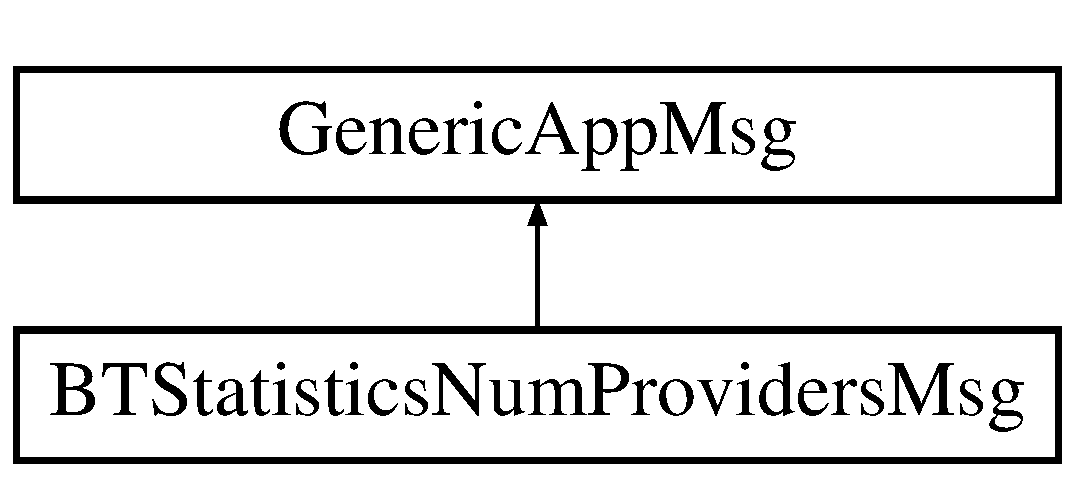
\includegraphics[height=2.000000cm]{classBTStatisticsNumProvidersMsg}
\end{center}
\end{figure}
\subsection*{Public Member Functions}
\begin{DoxyCompactItemize}
\item 
\hyperlink{classBTStatisticsNumProvidersMsg_a27c5fa76813c23277ade3648bee98f8a}{B\+T\+Statistics\+Num\+Providers\+Msg} (const char $\ast$name=N\+U\+L\+L, int kind=0)
\item 
\hyperlink{classBTStatisticsNumProvidersMsg_a37295adc4eddd651cfb4569f14c8df7f}{B\+T\+Statistics\+Num\+Providers\+Msg} (const \hyperlink{classBTStatisticsNumProvidersMsg}{B\+T\+Statistics\+Num\+Providers\+Msg} \&other)
\item 
virtual \hyperlink{classBTStatisticsNumProvidersMsg_a4fc1f39f4de311052f544e5273b85d3d}{$\sim$\+B\+T\+Statistics\+Num\+Providers\+Msg} ()
\item 
\hyperlink{classBTStatisticsNumProvidersMsg}{B\+T\+Statistics\+Num\+Providers\+Msg} \& \hyperlink{classBTStatisticsNumProvidersMsg_a217879768d37edfd58e4fa4b06a6de72}{operator=} (const \hyperlink{classBTStatisticsNumProvidersMsg}{B\+T\+Statistics\+Num\+Providers\+Msg} \&other)
\item 
virtual \hyperlink{classBTStatisticsNumProvidersMsg}{B\+T\+Statistics\+Num\+Providers\+Msg} $\ast$ \hyperlink{classBTStatisticsNumProvidersMsg_a8292a8314754ac51e96c36918600ebc4}{dup} () const 
\item 
virtual void \hyperlink{classBTStatisticsNumProvidersMsg_affef2efd7707ebeae624a2713cdcd2ff}{parsim\+Pack} (c\+Comm\+Buffer $\ast$b)
\item 
virtual void \hyperlink{classBTStatisticsNumProvidersMsg_a4864f751c4dc1a4186797eb9170cbc80}{parsim\+Unpack} (c\+Comm\+Buffer $\ast$b)
\item 
virtual int \hyperlink{classBTStatisticsNumProvidersMsg_a6a9306c19e6e47b66d630349696d0a42}{num\+Peers} () const 
\item 
virtual void \hyperlink{classBTStatisticsNumProvidersMsg_a56eb0c930bad9c15687db81ed15e9d47}{set\+Num\+Peers} (int \hyperlink{classBTStatisticsNumProvidersMsg_a245be09caa91893aebd3db42d5bc0e9d}{num\+Peers\+\_\+var})
\end{DoxyCompactItemize}
\subsection*{Protected Member Functions}
\begin{DoxyCompactItemize}
\item 
bool \hyperlink{classBTStatisticsNumProvidersMsg_acdef6ab3073f8bc86c11f72864b52eb6}{operator==} (const \hyperlink{classBTStatisticsNumProvidersMsg}{B\+T\+Statistics\+Num\+Providers\+Msg} \&)
\end{DoxyCompactItemize}
\subsection*{Protected Attributes}
\begin{DoxyCompactItemize}
\item 
int \hyperlink{classBTStatisticsNumProvidersMsg_a245be09caa91893aebd3db42d5bc0e9d}{num\+Peers\+\_\+var}
\end{DoxyCompactItemize}


\subsection{Detailed Description}
Class generated from {\ttfamily applications/x\+Bit\+Torrent/\+B\+T\+Statistics\+Msg.\+msg} by opp\+\_\+msgc. 
\begin{DoxyPre}
message \hyperlink{classBTStatisticsNumProvidersMsg}{BTStatisticsNumProvidersMsg} extends GenericAppMsg
\{
    (true);\end{DoxyPre}



\begin{DoxyPre}    int numPeers;
\}
\end{DoxyPre}
 

\subsection{Constructor \& Destructor Documentation}
\hypertarget{classBTStatisticsNumProvidersMsg_a27c5fa76813c23277ade3648bee98f8a}{}\index{B\+T\+Statistics\+Num\+Providers\+Msg@{B\+T\+Statistics\+Num\+Providers\+Msg}!B\+T\+Statistics\+Num\+Providers\+Msg@{B\+T\+Statistics\+Num\+Providers\+Msg}}
\index{B\+T\+Statistics\+Num\+Providers\+Msg@{B\+T\+Statistics\+Num\+Providers\+Msg}!B\+T\+Statistics\+Num\+Providers\+Msg@{B\+T\+Statistics\+Num\+Providers\+Msg}}
\subsubsection[{B\+T\+Statistics\+Num\+Providers\+Msg(const char $\ast$name=\+N\+U\+L\+L, int kind=0)}]{\setlength{\rightskip}{0pt plus 5cm}B\+T\+Statistics\+Num\+Providers\+Msg\+::\+B\+T\+Statistics\+Num\+Providers\+Msg (
\begin{DoxyParamCaption}
\item[{const char $\ast$}]{name = {\ttfamily NULL}, }
\item[{int}]{kind = {\ttfamily 0}}
\end{DoxyParamCaption}
)}\label{classBTStatisticsNumProvidersMsg_a27c5fa76813c23277ade3648bee98f8a}
\hypertarget{classBTStatisticsNumProvidersMsg_a37295adc4eddd651cfb4569f14c8df7f}{}\index{B\+T\+Statistics\+Num\+Providers\+Msg@{B\+T\+Statistics\+Num\+Providers\+Msg}!B\+T\+Statistics\+Num\+Providers\+Msg@{B\+T\+Statistics\+Num\+Providers\+Msg}}
\index{B\+T\+Statistics\+Num\+Providers\+Msg@{B\+T\+Statistics\+Num\+Providers\+Msg}!B\+T\+Statistics\+Num\+Providers\+Msg@{B\+T\+Statistics\+Num\+Providers\+Msg}}
\subsubsection[{B\+T\+Statistics\+Num\+Providers\+Msg(const B\+T\+Statistics\+Num\+Providers\+Msg \&other)}]{\setlength{\rightskip}{0pt plus 5cm}B\+T\+Statistics\+Num\+Providers\+Msg\+::\+B\+T\+Statistics\+Num\+Providers\+Msg (
\begin{DoxyParamCaption}
\item[{const {\bf B\+T\+Statistics\+Num\+Providers\+Msg} \&}]{other}
\end{DoxyParamCaption}
)}\label{classBTStatisticsNumProvidersMsg_a37295adc4eddd651cfb4569f14c8df7f}
\hypertarget{classBTStatisticsNumProvidersMsg_a4fc1f39f4de311052f544e5273b85d3d}{}\index{B\+T\+Statistics\+Num\+Providers\+Msg@{B\+T\+Statistics\+Num\+Providers\+Msg}!````~B\+T\+Statistics\+Num\+Providers\+Msg@{$\sim$\+B\+T\+Statistics\+Num\+Providers\+Msg}}
\index{````~B\+T\+Statistics\+Num\+Providers\+Msg@{$\sim$\+B\+T\+Statistics\+Num\+Providers\+Msg}!B\+T\+Statistics\+Num\+Providers\+Msg@{B\+T\+Statistics\+Num\+Providers\+Msg}}
\subsubsection[{$\sim$\+B\+T\+Statistics\+Num\+Providers\+Msg()}]{\setlength{\rightskip}{0pt plus 5cm}B\+T\+Statistics\+Num\+Providers\+Msg\+::$\sim$\+B\+T\+Statistics\+Num\+Providers\+Msg (
\begin{DoxyParamCaption}
{}
\end{DoxyParamCaption}
)\hspace{0.3cm}{\ttfamily [virtual]}}\label{classBTStatisticsNumProvidersMsg_a4fc1f39f4de311052f544e5273b85d3d}


\subsection{Member Function Documentation}
\hypertarget{classBTStatisticsNumProvidersMsg_a8292a8314754ac51e96c36918600ebc4}{}\index{B\+T\+Statistics\+Num\+Providers\+Msg@{B\+T\+Statistics\+Num\+Providers\+Msg}!dup@{dup}}
\index{dup@{dup}!B\+T\+Statistics\+Num\+Providers\+Msg@{B\+T\+Statistics\+Num\+Providers\+Msg}}
\subsubsection[{dup() const }]{\setlength{\rightskip}{0pt plus 5cm}virtual {\bf B\+T\+Statistics\+Num\+Providers\+Msg}$\ast$ B\+T\+Statistics\+Num\+Providers\+Msg\+::dup (
\begin{DoxyParamCaption}
{}
\end{DoxyParamCaption}
) const\hspace{0.3cm}{\ttfamily [inline]}, {\ttfamily [virtual]}}\label{classBTStatisticsNumProvidersMsg_a8292a8314754ac51e96c36918600ebc4}
\hypertarget{classBTStatisticsNumProvidersMsg_a6a9306c19e6e47b66d630349696d0a42}{}\index{B\+T\+Statistics\+Num\+Providers\+Msg@{B\+T\+Statistics\+Num\+Providers\+Msg}!num\+Peers@{num\+Peers}}
\index{num\+Peers@{num\+Peers}!B\+T\+Statistics\+Num\+Providers\+Msg@{B\+T\+Statistics\+Num\+Providers\+Msg}}
\subsubsection[{num\+Peers() const }]{\setlength{\rightskip}{0pt plus 5cm}int B\+T\+Statistics\+Num\+Providers\+Msg\+::num\+Peers (
\begin{DoxyParamCaption}
{}
\end{DoxyParamCaption}
) const\hspace{0.3cm}{\ttfamily [virtual]}}\label{classBTStatisticsNumProvidersMsg_a6a9306c19e6e47b66d630349696d0a42}
\hypertarget{classBTStatisticsNumProvidersMsg_a217879768d37edfd58e4fa4b06a6de72}{}\index{B\+T\+Statistics\+Num\+Providers\+Msg@{B\+T\+Statistics\+Num\+Providers\+Msg}!operator=@{operator=}}
\index{operator=@{operator=}!B\+T\+Statistics\+Num\+Providers\+Msg@{B\+T\+Statistics\+Num\+Providers\+Msg}}
\subsubsection[{operator=(const B\+T\+Statistics\+Num\+Providers\+Msg \&other)}]{\setlength{\rightskip}{0pt plus 5cm}{\bf B\+T\+Statistics\+Num\+Providers\+Msg} \& B\+T\+Statistics\+Num\+Providers\+Msg\+::operator= (
\begin{DoxyParamCaption}
\item[{const {\bf B\+T\+Statistics\+Num\+Providers\+Msg} \&}]{other}
\end{DoxyParamCaption}
)}\label{classBTStatisticsNumProvidersMsg_a217879768d37edfd58e4fa4b06a6de72}
\hypertarget{classBTStatisticsNumProvidersMsg_acdef6ab3073f8bc86c11f72864b52eb6}{}\index{B\+T\+Statistics\+Num\+Providers\+Msg@{B\+T\+Statistics\+Num\+Providers\+Msg}!operator==@{operator==}}
\index{operator==@{operator==}!B\+T\+Statistics\+Num\+Providers\+Msg@{B\+T\+Statistics\+Num\+Providers\+Msg}}
\subsubsection[{operator==(const B\+T\+Statistics\+Num\+Providers\+Msg \&)}]{\setlength{\rightskip}{0pt plus 5cm}bool B\+T\+Statistics\+Num\+Providers\+Msg\+::operator== (
\begin{DoxyParamCaption}
\item[{const {\bf B\+T\+Statistics\+Num\+Providers\+Msg} \&}]{}
\end{DoxyParamCaption}
)\hspace{0.3cm}{\ttfamily [protected]}}\label{classBTStatisticsNumProvidersMsg_acdef6ab3073f8bc86c11f72864b52eb6}
\hypertarget{classBTStatisticsNumProvidersMsg_affef2efd7707ebeae624a2713cdcd2ff}{}\index{B\+T\+Statistics\+Num\+Providers\+Msg@{B\+T\+Statistics\+Num\+Providers\+Msg}!parsim\+Pack@{parsim\+Pack}}
\index{parsim\+Pack@{parsim\+Pack}!B\+T\+Statistics\+Num\+Providers\+Msg@{B\+T\+Statistics\+Num\+Providers\+Msg}}
\subsubsection[{parsim\+Pack(c\+Comm\+Buffer $\ast$b)}]{\setlength{\rightskip}{0pt plus 5cm}void B\+T\+Statistics\+Num\+Providers\+Msg\+::parsim\+Pack (
\begin{DoxyParamCaption}
\item[{c\+Comm\+Buffer $\ast$}]{b}
\end{DoxyParamCaption}
)\hspace{0.3cm}{\ttfamily [virtual]}}\label{classBTStatisticsNumProvidersMsg_affef2efd7707ebeae624a2713cdcd2ff}
\hypertarget{classBTStatisticsNumProvidersMsg_a4864f751c4dc1a4186797eb9170cbc80}{}\index{B\+T\+Statistics\+Num\+Providers\+Msg@{B\+T\+Statistics\+Num\+Providers\+Msg}!parsim\+Unpack@{parsim\+Unpack}}
\index{parsim\+Unpack@{parsim\+Unpack}!B\+T\+Statistics\+Num\+Providers\+Msg@{B\+T\+Statistics\+Num\+Providers\+Msg}}
\subsubsection[{parsim\+Unpack(c\+Comm\+Buffer $\ast$b)}]{\setlength{\rightskip}{0pt plus 5cm}void B\+T\+Statistics\+Num\+Providers\+Msg\+::parsim\+Unpack (
\begin{DoxyParamCaption}
\item[{c\+Comm\+Buffer $\ast$}]{b}
\end{DoxyParamCaption}
)\hspace{0.3cm}{\ttfamily [virtual]}}\label{classBTStatisticsNumProvidersMsg_a4864f751c4dc1a4186797eb9170cbc80}
\hypertarget{classBTStatisticsNumProvidersMsg_a56eb0c930bad9c15687db81ed15e9d47}{}\index{B\+T\+Statistics\+Num\+Providers\+Msg@{B\+T\+Statistics\+Num\+Providers\+Msg}!set\+Num\+Peers@{set\+Num\+Peers}}
\index{set\+Num\+Peers@{set\+Num\+Peers}!B\+T\+Statistics\+Num\+Providers\+Msg@{B\+T\+Statistics\+Num\+Providers\+Msg}}
\subsubsection[{set\+Num\+Peers(int num\+Peers\+\_\+var)}]{\setlength{\rightskip}{0pt plus 5cm}void B\+T\+Statistics\+Num\+Providers\+Msg\+::set\+Num\+Peers (
\begin{DoxyParamCaption}
\item[{int}]{num\+Peers\+\_\+var}
\end{DoxyParamCaption}
)\hspace{0.3cm}{\ttfamily [virtual]}}\label{classBTStatisticsNumProvidersMsg_a56eb0c930bad9c15687db81ed15e9d47}


\subsection{Member Data Documentation}
\hypertarget{classBTStatisticsNumProvidersMsg_a245be09caa91893aebd3db42d5bc0e9d}{}\index{B\+T\+Statistics\+Num\+Providers\+Msg@{B\+T\+Statistics\+Num\+Providers\+Msg}!num\+Peers\+\_\+var@{num\+Peers\+\_\+var}}
\index{num\+Peers\+\_\+var@{num\+Peers\+\_\+var}!B\+T\+Statistics\+Num\+Providers\+Msg@{B\+T\+Statistics\+Num\+Providers\+Msg}}
\subsubsection[{num\+Peers\+\_\+var}]{\setlength{\rightskip}{0pt plus 5cm}int B\+T\+Statistics\+Num\+Providers\+Msg\+::num\+Peers\+\_\+var\hspace{0.3cm}{\ttfamily [protected]}}\label{classBTStatisticsNumProvidersMsg_a245be09caa91893aebd3db42d5bc0e9d}


The documentation for this class was generated from the following files\+:\begin{DoxyCompactItemize}
\item 
\hyperlink{BTStatisticsMsg__m_8h}{B\+T\+Statistics\+Msg\+\_\+m.\+h}\item 
\hyperlink{BTStatisticsMsg__m_8cc}{B\+T\+Statistics\+Msg\+\_\+m.\+cc}\end{DoxyCompactItemize}

\hypertarget{classBTStatisticsNumProvidersMsgDescriptor}{}\section{B\+T\+Statistics\+Num\+Providers\+Msg\+Descriptor Class Reference}
\label{classBTStatisticsNumProvidersMsgDescriptor}\index{B\+T\+Statistics\+Num\+Providers\+Msg\+Descriptor@{B\+T\+Statistics\+Num\+Providers\+Msg\+Descriptor}}
Inheritance diagram for B\+T\+Statistics\+Num\+Providers\+Msg\+Descriptor\+:\begin{figure}[H]
\begin{center}
\leavevmode
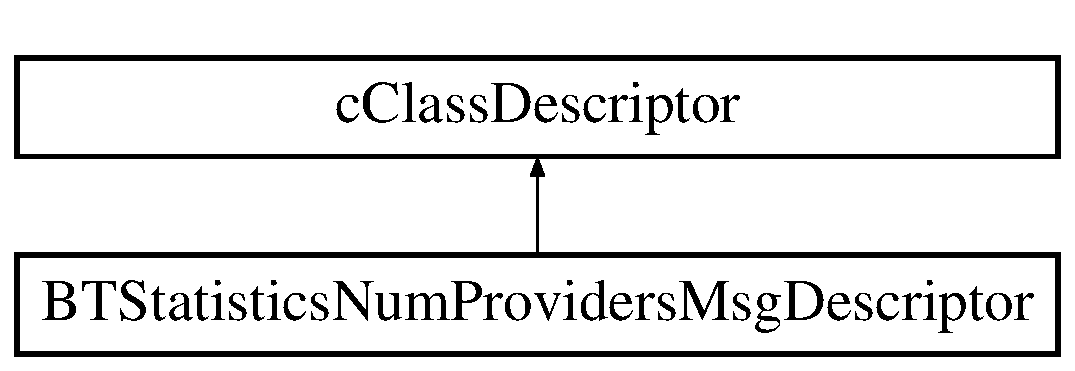
\includegraphics[height=2.000000cm]{classBTStatisticsNumProvidersMsgDescriptor}
\end{center}
\end{figure}
\subsection*{Public Member Functions}
\begin{DoxyCompactItemize}
\item 
\hyperlink{classBTStatisticsNumProvidersMsgDescriptor_a6bceac3ad7bb634e3ee1a85156dc7524}{B\+T\+Statistics\+Num\+Providers\+Msg\+Descriptor} ()
\item 
virtual \hyperlink{classBTStatisticsNumProvidersMsgDescriptor_a0d2d1a8cbd91dc37741ecbddbb986e54}{$\sim$\+B\+T\+Statistics\+Num\+Providers\+Msg\+Descriptor} ()
\item 
virtual bool \hyperlink{classBTStatisticsNumProvidersMsgDescriptor_a4140af5b4d771f52e47d645675891a77}{does\+Support} (c\+Object $\ast$obj) const 
\item 
virtual const char $\ast$ \hyperlink{classBTStatisticsNumProvidersMsgDescriptor_ac0b00a1d046cc8e0e106abc4297c082a}{get\+Property} (const char $\ast$propertyname) const 
\item 
virtual int \hyperlink{classBTStatisticsNumProvidersMsgDescriptor_a94e59af862bad393266dab838ff3e94b}{get\+Field\+Count} (void $\ast$object) const 
\item 
virtual const char $\ast$ \hyperlink{classBTStatisticsNumProvidersMsgDescriptor_a129ffdb57624b98e377393985c5c370b}{get\+Field\+Name} (void $\ast$object, int field) const 
\item 
virtual int \hyperlink{classBTStatisticsNumProvidersMsgDescriptor_ae61c49208e0a400b707b49d3690ab8c1}{find\+Field} (void $\ast$object, const char $\ast$field\+Name) const 
\item 
virtual unsigned int \hyperlink{classBTStatisticsNumProvidersMsgDescriptor_ae8a24bd14f51c5a4e430d72f24baa7a4}{get\+Field\+Type\+Flags} (void $\ast$object, int field) const 
\item 
virtual const char $\ast$ \hyperlink{classBTStatisticsNumProvidersMsgDescriptor_aec1d5d249cfb413c8f8cca0f8ae76392}{get\+Field\+Type\+String} (void $\ast$object, int field) const 
\item 
virtual const char $\ast$ \hyperlink{classBTStatisticsNumProvidersMsgDescriptor_a137e1080f841f8df336325f458ae801c}{get\+Field\+Property} (void $\ast$object, int field, const char $\ast$propertyname) const 
\item 
virtual int \hyperlink{classBTStatisticsNumProvidersMsgDescriptor_aca292acecda6b63aff572701196c8033}{get\+Array\+Size} (void $\ast$object, int field) const 
\item 
virtual std\+::string \hyperlink{classBTStatisticsNumProvidersMsgDescriptor_a68d60317b7825355cddfcf1f7b4a0553}{get\+Field\+As\+String} (void $\ast$object, int field, int i) const 
\item 
virtual bool \hyperlink{classBTStatisticsNumProvidersMsgDescriptor_a21420b324353995023c5f511ae7287f4}{set\+Field\+As\+String} (void $\ast$object, int field, int i, const char $\ast$value) const 
\item 
virtual const char $\ast$ \hyperlink{classBTStatisticsNumProvidersMsgDescriptor_a3e22d75d38c71ed2e4c438d52497b7c4}{get\+Field\+Struct\+Name} (void $\ast$object, int field) const 
\item 
virtual void $\ast$ \hyperlink{classBTStatisticsNumProvidersMsgDescriptor_a282b6484059387faff8a0534019cdd78}{get\+Field\+Struct\+Pointer} (void $\ast$object, int field, int i) const 
\end{DoxyCompactItemize}


\subsection{Constructor \& Destructor Documentation}
\hypertarget{classBTStatisticsNumProvidersMsgDescriptor_a6bceac3ad7bb634e3ee1a85156dc7524}{}\index{B\+T\+Statistics\+Num\+Providers\+Msg\+Descriptor@{B\+T\+Statistics\+Num\+Providers\+Msg\+Descriptor}!B\+T\+Statistics\+Num\+Providers\+Msg\+Descriptor@{B\+T\+Statistics\+Num\+Providers\+Msg\+Descriptor}}
\index{B\+T\+Statistics\+Num\+Providers\+Msg\+Descriptor@{B\+T\+Statistics\+Num\+Providers\+Msg\+Descriptor}!B\+T\+Statistics\+Num\+Providers\+Msg\+Descriptor@{B\+T\+Statistics\+Num\+Providers\+Msg\+Descriptor}}
\subsubsection[{B\+T\+Statistics\+Num\+Providers\+Msg\+Descriptor()}]{\setlength{\rightskip}{0pt plus 5cm}B\+T\+Statistics\+Num\+Providers\+Msg\+Descriptor\+::\+B\+T\+Statistics\+Num\+Providers\+Msg\+Descriptor (
\begin{DoxyParamCaption}
{}
\end{DoxyParamCaption}
)}\label{classBTStatisticsNumProvidersMsgDescriptor_a6bceac3ad7bb634e3ee1a85156dc7524}
\hypertarget{classBTStatisticsNumProvidersMsgDescriptor_a0d2d1a8cbd91dc37741ecbddbb986e54}{}\index{B\+T\+Statistics\+Num\+Providers\+Msg\+Descriptor@{B\+T\+Statistics\+Num\+Providers\+Msg\+Descriptor}!````~B\+T\+Statistics\+Num\+Providers\+Msg\+Descriptor@{$\sim$\+B\+T\+Statistics\+Num\+Providers\+Msg\+Descriptor}}
\index{````~B\+T\+Statistics\+Num\+Providers\+Msg\+Descriptor@{$\sim$\+B\+T\+Statistics\+Num\+Providers\+Msg\+Descriptor}!B\+T\+Statistics\+Num\+Providers\+Msg\+Descriptor@{B\+T\+Statistics\+Num\+Providers\+Msg\+Descriptor}}
\subsubsection[{$\sim$\+B\+T\+Statistics\+Num\+Providers\+Msg\+Descriptor()}]{\setlength{\rightskip}{0pt plus 5cm}B\+T\+Statistics\+Num\+Providers\+Msg\+Descriptor\+::$\sim$\+B\+T\+Statistics\+Num\+Providers\+Msg\+Descriptor (
\begin{DoxyParamCaption}
{}
\end{DoxyParamCaption}
)\hspace{0.3cm}{\ttfamily [virtual]}}\label{classBTStatisticsNumProvidersMsgDescriptor_a0d2d1a8cbd91dc37741ecbddbb986e54}


\subsection{Member Function Documentation}
\hypertarget{classBTStatisticsNumProvidersMsgDescriptor_a4140af5b4d771f52e47d645675891a77}{}\index{B\+T\+Statistics\+Num\+Providers\+Msg\+Descriptor@{B\+T\+Statistics\+Num\+Providers\+Msg\+Descriptor}!does\+Support@{does\+Support}}
\index{does\+Support@{does\+Support}!B\+T\+Statistics\+Num\+Providers\+Msg\+Descriptor@{B\+T\+Statistics\+Num\+Providers\+Msg\+Descriptor}}
\subsubsection[{does\+Support(c\+Object $\ast$obj) const }]{\setlength{\rightskip}{0pt plus 5cm}bool B\+T\+Statistics\+Num\+Providers\+Msg\+Descriptor\+::does\+Support (
\begin{DoxyParamCaption}
\item[{c\+Object $\ast$}]{obj}
\end{DoxyParamCaption}
) const\hspace{0.3cm}{\ttfamily [virtual]}}\label{classBTStatisticsNumProvidersMsgDescriptor_a4140af5b4d771f52e47d645675891a77}
\hypertarget{classBTStatisticsNumProvidersMsgDescriptor_ae61c49208e0a400b707b49d3690ab8c1}{}\index{B\+T\+Statistics\+Num\+Providers\+Msg\+Descriptor@{B\+T\+Statistics\+Num\+Providers\+Msg\+Descriptor}!find\+Field@{find\+Field}}
\index{find\+Field@{find\+Field}!B\+T\+Statistics\+Num\+Providers\+Msg\+Descriptor@{B\+T\+Statistics\+Num\+Providers\+Msg\+Descriptor}}
\subsubsection[{find\+Field(void $\ast$object, const char $\ast$field\+Name) const }]{\setlength{\rightskip}{0pt plus 5cm}int B\+T\+Statistics\+Num\+Providers\+Msg\+Descriptor\+::find\+Field (
\begin{DoxyParamCaption}
\item[{void $\ast$}]{object, }
\item[{const char $\ast$}]{field\+Name}
\end{DoxyParamCaption}
) const\hspace{0.3cm}{\ttfamily [virtual]}}\label{classBTStatisticsNumProvidersMsgDescriptor_ae61c49208e0a400b707b49d3690ab8c1}
\hypertarget{classBTStatisticsNumProvidersMsgDescriptor_aca292acecda6b63aff572701196c8033}{}\index{B\+T\+Statistics\+Num\+Providers\+Msg\+Descriptor@{B\+T\+Statistics\+Num\+Providers\+Msg\+Descriptor}!get\+Array\+Size@{get\+Array\+Size}}
\index{get\+Array\+Size@{get\+Array\+Size}!B\+T\+Statistics\+Num\+Providers\+Msg\+Descriptor@{B\+T\+Statistics\+Num\+Providers\+Msg\+Descriptor}}
\subsubsection[{get\+Array\+Size(void $\ast$object, int field) const }]{\setlength{\rightskip}{0pt plus 5cm}int B\+T\+Statistics\+Num\+Providers\+Msg\+Descriptor\+::get\+Array\+Size (
\begin{DoxyParamCaption}
\item[{void $\ast$}]{object, }
\item[{int}]{field}
\end{DoxyParamCaption}
) const\hspace{0.3cm}{\ttfamily [virtual]}}\label{classBTStatisticsNumProvidersMsgDescriptor_aca292acecda6b63aff572701196c8033}
\hypertarget{classBTStatisticsNumProvidersMsgDescriptor_a68d60317b7825355cddfcf1f7b4a0553}{}\index{B\+T\+Statistics\+Num\+Providers\+Msg\+Descriptor@{B\+T\+Statistics\+Num\+Providers\+Msg\+Descriptor}!get\+Field\+As\+String@{get\+Field\+As\+String}}
\index{get\+Field\+As\+String@{get\+Field\+As\+String}!B\+T\+Statistics\+Num\+Providers\+Msg\+Descriptor@{B\+T\+Statistics\+Num\+Providers\+Msg\+Descriptor}}
\subsubsection[{get\+Field\+As\+String(void $\ast$object, int field, int i) const }]{\setlength{\rightskip}{0pt plus 5cm}std\+::string B\+T\+Statistics\+Num\+Providers\+Msg\+Descriptor\+::get\+Field\+As\+String (
\begin{DoxyParamCaption}
\item[{void $\ast$}]{object, }
\item[{int}]{field, }
\item[{int}]{i}
\end{DoxyParamCaption}
) const\hspace{0.3cm}{\ttfamily [virtual]}}\label{classBTStatisticsNumProvidersMsgDescriptor_a68d60317b7825355cddfcf1f7b4a0553}
\hypertarget{classBTStatisticsNumProvidersMsgDescriptor_a94e59af862bad393266dab838ff3e94b}{}\index{B\+T\+Statistics\+Num\+Providers\+Msg\+Descriptor@{B\+T\+Statistics\+Num\+Providers\+Msg\+Descriptor}!get\+Field\+Count@{get\+Field\+Count}}
\index{get\+Field\+Count@{get\+Field\+Count}!B\+T\+Statistics\+Num\+Providers\+Msg\+Descriptor@{B\+T\+Statistics\+Num\+Providers\+Msg\+Descriptor}}
\subsubsection[{get\+Field\+Count(void $\ast$object) const }]{\setlength{\rightskip}{0pt plus 5cm}int B\+T\+Statistics\+Num\+Providers\+Msg\+Descriptor\+::get\+Field\+Count (
\begin{DoxyParamCaption}
\item[{void $\ast$}]{object}
\end{DoxyParamCaption}
) const\hspace{0.3cm}{\ttfamily [virtual]}}\label{classBTStatisticsNumProvidersMsgDescriptor_a94e59af862bad393266dab838ff3e94b}
\hypertarget{classBTStatisticsNumProvidersMsgDescriptor_a129ffdb57624b98e377393985c5c370b}{}\index{B\+T\+Statistics\+Num\+Providers\+Msg\+Descriptor@{B\+T\+Statistics\+Num\+Providers\+Msg\+Descriptor}!get\+Field\+Name@{get\+Field\+Name}}
\index{get\+Field\+Name@{get\+Field\+Name}!B\+T\+Statistics\+Num\+Providers\+Msg\+Descriptor@{B\+T\+Statistics\+Num\+Providers\+Msg\+Descriptor}}
\subsubsection[{get\+Field\+Name(void $\ast$object, int field) const }]{\setlength{\rightskip}{0pt plus 5cm}const char $\ast$ B\+T\+Statistics\+Num\+Providers\+Msg\+Descriptor\+::get\+Field\+Name (
\begin{DoxyParamCaption}
\item[{void $\ast$}]{object, }
\item[{int}]{field}
\end{DoxyParamCaption}
) const\hspace{0.3cm}{\ttfamily [virtual]}}\label{classBTStatisticsNumProvidersMsgDescriptor_a129ffdb57624b98e377393985c5c370b}
\hypertarget{classBTStatisticsNumProvidersMsgDescriptor_a137e1080f841f8df336325f458ae801c}{}\index{B\+T\+Statistics\+Num\+Providers\+Msg\+Descriptor@{B\+T\+Statistics\+Num\+Providers\+Msg\+Descriptor}!get\+Field\+Property@{get\+Field\+Property}}
\index{get\+Field\+Property@{get\+Field\+Property}!B\+T\+Statistics\+Num\+Providers\+Msg\+Descriptor@{B\+T\+Statistics\+Num\+Providers\+Msg\+Descriptor}}
\subsubsection[{get\+Field\+Property(void $\ast$object, int field, const char $\ast$propertyname) const }]{\setlength{\rightskip}{0pt plus 5cm}const char $\ast$ B\+T\+Statistics\+Num\+Providers\+Msg\+Descriptor\+::get\+Field\+Property (
\begin{DoxyParamCaption}
\item[{void $\ast$}]{object, }
\item[{int}]{field, }
\item[{const char $\ast$}]{propertyname}
\end{DoxyParamCaption}
) const\hspace{0.3cm}{\ttfamily [virtual]}}\label{classBTStatisticsNumProvidersMsgDescriptor_a137e1080f841f8df336325f458ae801c}
\hypertarget{classBTStatisticsNumProvidersMsgDescriptor_a3e22d75d38c71ed2e4c438d52497b7c4}{}\index{B\+T\+Statistics\+Num\+Providers\+Msg\+Descriptor@{B\+T\+Statistics\+Num\+Providers\+Msg\+Descriptor}!get\+Field\+Struct\+Name@{get\+Field\+Struct\+Name}}
\index{get\+Field\+Struct\+Name@{get\+Field\+Struct\+Name}!B\+T\+Statistics\+Num\+Providers\+Msg\+Descriptor@{B\+T\+Statistics\+Num\+Providers\+Msg\+Descriptor}}
\subsubsection[{get\+Field\+Struct\+Name(void $\ast$object, int field) const }]{\setlength{\rightskip}{0pt plus 5cm}const char $\ast$ B\+T\+Statistics\+Num\+Providers\+Msg\+Descriptor\+::get\+Field\+Struct\+Name (
\begin{DoxyParamCaption}
\item[{void $\ast$}]{object, }
\item[{int}]{field}
\end{DoxyParamCaption}
) const\hspace{0.3cm}{\ttfamily [virtual]}}\label{classBTStatisticsNumProvidersMsgDescriptor_a3e22d75d38c71ed2e4c438d52497b7c4}
\hypertarget{classBTStatisticsNumProvidersMsgDescriptor_a282b6484059387faff8a0534019cdd78}{}\index{B\+T\+Statistics\+Num\+Providers\+Msg\+Descriptor@{B\+T\+Statistics\+Num\+Providers\+Msg\+Descriptor}!get\+Field\+Struct\+Pointer@{get\+Field\+Struct\+Pointer}}
\index{get\+Field\+Struct\+Pointer@{get\+Field\+Struct\+Pointer}!B\+T\+Statistics\+Num\+Providers\+Msg\+Descriptor@{B\+T\+Statistics\+Num\+Providers\+Msg\+Descriptor}}
\subsubsection[{get\+Field\+Struct\+Pointer(void $\ast$object, int field, int i) const }]{\setlength{\rightskip}{0pt plus 5cm}void $\ast$ B\+T\+Statistics\+Num\+Providers\+Msg\+Descriptor\+::get\+Field\+Struct\+Pointer (
\begin{DoxyParamCaption}
\item[{void $\ast$}]{object, }
\item[{int}]{field, }
\item[{int}]{i}
\end{DoxyParamCaption}
) const\hspace{0.3cm}{\ttfamily [virtual]}}\label{classBTStatisticsNumProvidersMsgDescriptor_a282b6484059387faff8a0534019cdd78}
\hypertarget{classBTStatisticsNumProvidersMsgDescriptor_ae8a24bd14f51c5a4e430d72f24baa7a4}{}\index{B\+T\+Statistics\+Num\+Providers\+Msg\+Descriptor@{B\+T\+Statistics\+Num\+Providers\+Msg\+Descriptor}!get\+Field\+Type\+Flags@{get\+Field\+Type\+Flags}}
\index{get\+Field\+Type\+Flags@{get\+Field\+Type\+Flags}!B\+T\+Statistics\+Num\+Providers\+Msg\+Descriptor@{B\+T\+Statistics\+Num\+Providers\+Msg\+Descriptor}}
\subsubsection[{get\+Field\+Type\+Flags(void $\ast$object, int field) const }]{\setlength{\rightskip}{0pt plus 5cm}unsigned int B\+T\+Statistics\+Num\+Providers\+Msg\+Descriptor\+::get\+Field\+Type\+Flags (
\begin{DoxyParamCaption}
\item[{void $\ast$}]{object, }
\item[{int}]{field}
\end{DoxyParamCaption}
) const\hspace{0.3cm}{\ttfamily [virtual]}}\label{classBTStatisticsNumProvidersMsgDescriptor_ae8a24bd14f51c5a4e430d72f24baa7a4}
\hypertarget{classBTStatisticsNumProvidersMsgDescriptor_aec1d5d249cfb413c8f8cca0f8ae76392}{}\index{B\+T\+Statistics\+Num\+Providers\+Msg\+Descriptor@{B\+T\+Statistics\+Num\+Providers\+Msg\+Descriptor}!get\+Field\+Type\+String@{get\+Field\+Type\+String}}
\index{get\+Field\+Type\+String@{get\+Field\+Type\+String}!B\+T\+Statistics\+Num\+Providers\+Msg\+Descriptor@{B\+T\+Statistics\+Num\+Providers\+Msg\+Descriptor}}
\subsubsection[{get\+Field\+Type\+String(void $\ast$object, int field) const }]{\setlength{\rightskip}{0pt plus 5cm}const char $\ast$ B\+T\+Statistics\+Num\+Providers\+Msg\+Descriptor\+::get\+Field\+Type\+String (
\begin{DoxyParamCaption}
\item[{void $\ast$}]{object, }
\item[{int}]{field}
\end{DoxyParamCaption}
) const\hspace{0.3cm}{\ttfamily [virtual]}}\label{classBTStatisticsNumProvidersMsgDescriptor_aec1d5d249cfb413c8f8cca0f8ae76392}
\hypertarget{classBTStatisticsNumProvidersMsgDescriptor_ac0b00a1d046cc8e0e106abc4297c082a}{}\index{B\+T\+Statistics\+Num\+Providers\+Msg\+Descriptor@{B\+T\+Statistics\+Num\+Providers\+Msg\+Descriptor}!get\+Property@{get\+Property}}
\index{get\+Property@{get\+Property}!B\+T\+Statistics\+Num\+Providers\+Msg\+Descriptor@{B\+T\+Statistics\+Num\+Providers\+Msg\+Descriptor}}
\subsubsection[{get\+Property(const char $\ast$propertyname) const }]{\setlength{\rightskip}{0pt plus 5cm}const char $\ast$ B\+T\+Statistics\+Num\+Providers\+Msg\+Descriptor\+::get\+Property (
\begin{DoxyParamCaption}
\item[{const char $\ast$}]{propertyname}
\end{DoxyParamCaption}
) const\hspace{0.3cm}{\ttfamily [virtual]}}\label{classBTStatisticsNumProvidersMsgDescriptor_ac0b00a1d046cc8e0e106abc4297c082a}
\hypertarget{classBTStatisticsNumProvidersMsgDescriptor_a21420b324353995023c5f511ae7287f4}{}\index{B\+T\+Statistics\+Num\+Providers\+Msg\+Descriptor@{B\+T\+Statistics\+Num\+Providers\+Msg\+Descriptor}!set\+Field\+As\+String@{set\+Field\+As\+String}}
\index{set\+Field\+As\+String@{set\+Field\+As\+String}!B\+T\+Statistics\+Num\+Providers\+Msg\+Descriptor@{B\+T\+Statistics\+Num\+Providers\+Msg\+Descriptor}}
\subsubsection[{set\+Field\+As\+String(void $\ast$object, int field, int i, const char $\ast$value) const }]{\setlength{\rightskip}{0pt plus 5cm}bool B\+T\+Statistics\+Num\+Providers\+Msg\+Descriptor\+::set\+Field\+As\+String (
\begin{DoxyParamCaption}
\item[{void $\ast$}]{object, }
\item[{int}]{field, }
\item[{int}]{i, }
\item[{const char $\ast$}]{value}
\end{DoxyParamCaption}
) const\hspace{0.3cm}{\ttfamily [virtual]}}\label{classBTStatisticsNumProvidersMsgDescriptor_a21420b324353995023c5f511ae7287f4}


The documentation for this class was generated from the following file\+:\begin{DoxyCompactItemize}
\item 
\hyperlink{BTStatisticsMsg__m_8cc}{B\+T\+Statistics\+Msg\+\_\+m.\+cc}\end{DoxyCompactItemize}

\hypertarget{classBTStatisticsNumSeederBlocksMsg}{}\section{B\+T\+Statistics\+Num\+Seeder\+Blocks\+Msg Class Reference}
\label{classBTStatisticsNumSeederBlocksMsg}\index{B\+T\+Statistics\+Num\+Seeder\+Blocks\+Msg@{B\+T\+Statistics\+Num\+Seeder\+Blocks\+Msg}}


{\ttfamily \#include $<$B\+T\+Statistics\+Msg\+\_\+m.\+h$>$}

Inheritance diagram for B\+T\+Statistics\+Num\+Seeder\+Blocks\+Msg\+:\begin{figure}[H]
\begin{center}
\leavevmode
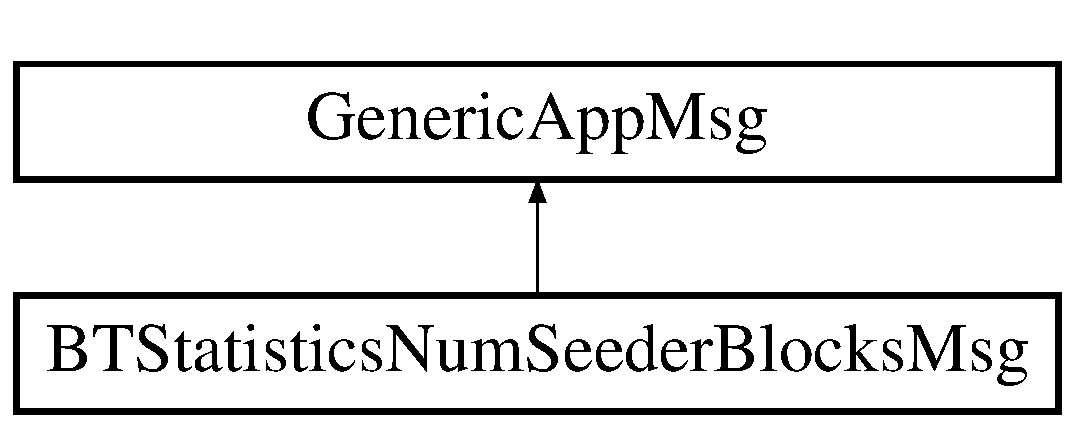
\includegraphics[height=2.000000cm]{classBTStatisticsNumSeederBlocksMsg}
\end{center}
\end{figure}
\subsection*{Public Member Functions}
\begin{DoxyCompactItemize}
\item 
\hyperlink{classBTStatisticsNumSeederBlocksMsg_a5d2af03243461bb5b98846d2c522ad66}{B\+T\+Statistics\+Num\+Seeder\+Blocks\+Msg} (const char $\ast$name=N\+U\+L\+L, int kind=0)
\item 
\hyperlink{classBTStatisticsNumSeederBlocksMsg_a529b5bd96bb11e7e88771902aef0cfbc}{B\+T\+Statistics\+Num\+Seeder\+Blocks\+Msg} (const \hyperlink{classBTStatisticsNumSeederBlocksMsg}{B\+T\+Statistics\+Num\+Seeder\+Blocks\+Msg} \&other)
\item 
virtual \hyperlink{classBTStatisticsNumSeederBlocksMsg_ab3c47ce19884582b74479978f0127c5e}{$\sim$\+B\+T\+Statistics\+Num\+Seeder\+Blocks\+Msg} ()
\item 
\hyperlink{classBTStatisticsNumSeederBlocksMsg}{B\+T\+Statistics\+Num\+Seeder\+Blocks\+Msg} \& \hyperlink{classBTStatisticsNumSeederBlocksMsg_a9b079f428f2992996abdd7f8d9efe0aa}{operator=} (const \hyperlink{classBTStatisticsNumSeederBlocksMsg}{B\+T\+Statistics\+Num\+Seeder\+Blocks\+Msg} \&other)
\item 
virtual \hyperlink{classBTStatisticsNumSeederBlocksMsg}{B\+T\+Statistics\+Num\+Seeder\+Blocks\+Msg} $\ast$ \hyperlink{classBTStatisticsNumSeederBlocksMsg_a44044a4c7f90c3efba1bef8718f1e4ff}{dup} () const 
\item 
virtual void \hyperlink{classBTStatisticsNumSeederBlocksMsg_a88a03ef916580cf6444af39b99ddf5ed}{parsim\+Pack} (c\+Comm\+Buffer $\ast$b)
\item 
virtual void \hyperlink{classBTStatisticsNumSeederBlocksMsg_a84b8cc5dbc283c4b78c8690bb132c2a3}{parsim\+Unpack} (c\+Comm\+Buffer $\ast$b)
\item 
virtual double \hyperlink{classBTStatisticsNumSeederBlocksMsg_a3cc398947135cbcc744dff2f3b3a8acc}{num\+Seeder\+Blocks} () const 
\item 
virtual void \hyperlink{classBTStatisticsNumSeederBlocksMsg_a22e498f7170b1cee325e3bfccf90d512}{set\+Num\+Seeder\+Blocks} (double \hyperlink{classBTStatisticsNumSeederBlocksMsg_a58db53e8c0c42406ba090ecc6bc0cd11}{num\+Seeder\+Blocks\+\_\+var})
\end{DoxyCompactItemize}
\subsection*{Protected Member Functions}
\begin{DoxyCompactItemize}
\item 
bool \hyperlink{classBTStatisticsNumSeederBlocksMsg_afdff1f716ba69718851cc1a2c4bd731a}{operator==} (const \hyperlink{classBTStatisticsNumSeederBlocksMsg}{B\+T\+Statistics\+Num\+Seeder\+Blocks\+Msg} \&)
\end{DoxyCompactItemize}
\subsection*{Protected Attributes}
\begin{DoxyCompactItemize}
\item 
double \hyperlink{classBTStatisticsNumSeederBlocksMsg_a58db53e8c0c42406ba090ecc6bc0cd11}{num\+Seeder\+Blocks\+\_\+var}
\end{DoxyCompactItemize}


\subsection{Detailed Description}
Class generated from {\ttfamily applications/x\+Bit\+Torrent/\+B\+T\+Statistics\+Msg.\+msg} by opp\+\_\+msgc. 
\begin{DoxyPre}
message \hyperlink{classBTStatisticsNumSeederBlocksMsg}{BTStatisticsNumSeederBlocksMsg} extends GenericAppMsg
\{
    (true);\end{DoxyPre}



\begin{DoxyPre}    double numSeederBlocks;
\}
\end{DoxyPre}
 

\subsection{Constructor \& Destructor Documentation}
\hypertarget{classBTStatisticsNumSeederBlocksMsg_a5d2af03243461bb5b98846d2c522ad66}{}\index{B\+T\+Statistics\+Num\+Seeder\+Blocks\+Msg@{B\+T\+Statistics\+Num\+Seeder\+Blocks\+Msg}!B\+T\+Statistics\+Num\+Seeder\+Blocks\+Msg@{B\+T\+Statistics\+Num\+Seeder\+Blocks\+Msg}}
\index{B\+T\+Statistics\+Num\+Seeder\+Blocks\+Msg@{B\+T\+Statistics\+Num\+Seeder\+Blocks\+Msg}!B\+T\+Statistics\+Num\+Seeder\+Blocks\+Msg@{B\+T\+Statistics\+Num\+Seeder\+Blocks\+Msg}}
\subsubsection[{B\+T\+Statistics\+Num\+Seeder\+Blocks\+Msg(const char $\ast$name=\+N\+U\+L\+L, int kind=0)}]{\setlength{\rightskip}{0pt plus 5cm}B\+T\+Statistics\+Num\+Seeder\+Blocks\+Msg\+::\+B\+T\+Statistics\+Num\+Seeder\+Blocks\+Msg (
\begin{DoxyParamCaption}
\item[{const char $\ast$}]{name = {\ttfamily NULL}, }
\item[{int}]{kind = {\ttfamily 0}}
\end{DoxyParamCaption}
)}\label{classBTStatisticsNumSeederBlocksMsg_a5d2af03243461bb5b98846d2c522ad66}
\hypertarget{classBTStatisticsNumSeederBlocksMsg_a529b5bd96bb11e7e88771902aef0cfbc}{}\index{B\+T\+Statistics\+Num\+Seeder\+Blocks\+Msg@{B\+T\+Statistics\+Num\+Seeder\+Blocks\+Msg}!B\+T\+Statistics\+Num\+Seeder\+Blocks\+Msg@{B\+T\+Statistics\+Num\+Seeder\+Blocks\+Msg}}
\index{B\+T\+Statistics\+Num\+Seeder\+Blocks\+Msg@{B\+T\+Statistics\+Num\+Seeder\+Blocks\+Msg}!B\+T\+Statistics\+Num\+Seeder\+Blocks\+Msg@{B\+T\+Statistics\+Num\+Seeder\+Blocks\+Msg}}
\subsubsection[{B\+T\+Statistics\+Num\+Seeder\+Blocks\+Msg(const B\+T\+Statistics\+Num\+Seeder\+Blocks\+Msg \&other)}]{\setlength{\rightskip}{0pt plus 5cm}B\+T\+Statistics\+Num\+Seeder\+Blocks\+Msg\+::\+B\+T\+Statistics\+Num\+Seeder\+Blocks\+Msg (
\begin{DoxyParamCaption}
\item[{const {\bf B\+T\+Statistics\+Num\+Seeder\+Blocks\+Msg} \&}]{other}
\end{DoxyParamCaption}
)}\label{classBTStatisticsNumSeederBlocksMsg_a529b5bd96bb11e7e88771902aef0cfbc}
\hypertarget{classBTStatisticsNumSeederBlocksMsg_ab3c47ce19884582b74479978f0127c5e}{}\index{B\+T\+Statistics\+Num\+Seeder\+Blocks\+Msg@{B\+T\+Statistics\+Num\+Seeder\+Blocks\+Msg}!````~B\+T\+Statistics\+Num\+Seeder\+Blocks\+Msg@{$\sim$\+B\+T\+Statistics\+Num\+Seeder\+Blocks\+Msg}}
\index{````~B\+T\+Statistics\+Num\+Seeder\+Blocks\+Msg@{$\sim$\+B\+T\+Statistics\+Num\+Seeder\+Blocks\+Msg}!B\+T\+Statistics\+Num\+Seeder\+Blocks\+Msg@{B\+T\+Statistics\+Num\+Seeder\+Blocks\+Msg}}
\subsubsection[{$\sim$\+B\+T\+Statistics\+Num\+Seeder\+Blocks\+Msg()}]{\setlength{\rightskip}{0pt plus 5cm}B\+T\+Statistics\+Num\+Seeder\+Blocks\+Msg\+::$\sim$\+B\+T\+Statistics\+Num\+Seeder\+Blocks\+Msg (
\begin{DoxyParamCaption}
{}
\end{DoxyParamCaption}
)\hspace{0.3cm}{\ttfamily [virtual]}}\label{classBTStatisticsNumSeederBlocksMsg_ab3c47ce19884582b74479978f0127c5e}


\subsection{Member Function Documentation}
\hypertarget{classBTStatisticsNumSeederBlocksMsg_a44044a4c7f90c3efba1bef8718f1e4ff}{}\index{B\+T\+Statistics\+Num\+Seeder\+Blocks\+Msg@{B\+T\+Statistics\+Num\+Seeder\+Blocks\+Msg}!dup@{dup}}
\index{dup@{dup}!B\+T\+Statistics\+Num\+Seeder\+Blocks\+Msg@{B\+T\+Statistics\+Num\+Seeder\+Blocks\+Msg}}
\subsubsection[{dup() const }]{\setlength{\rightskip}{0pt plus 5cm}virtual {\bf B\+T\+Statistics\+Num\+Seeder\+Blocks\+Msg}$\ast$ B\+T\+Statistics\+Num\+Seeder\+Blocks\+Msg\+::dup (
\begin{DoxyParamCaption}
{}
\end{DoxyParamCaption}
) const\hspace{0.3cm}{\ttfamily [inline]}, {\ttfamily [virtual]}}\label{classBTStatisticsNumSeederBlocksMsg_a44044a4c7f90c3efba1bef8718f1e4ff}
\hypertarget{classBTStatisticsNumSeederBlocksMsg_a3cc398947135cbcc744dff2f3b3a8acc}{}\index{B\+T\+Statistics\+Num\+Seeder\+Blocks\+Msg@{B\+T\+Statistics\+Num\+Seeder\+Blocks\+Msg}!num\+Seeder\+Blocks@{num\+Seeder\+Blocks}}
\index{num\+Seeder\+Blocks@{num\+Seeder\+Blocks}!B\+T\+Statistics\+Num\+Seeder\+Blocks\+Msg@{B\+T\+Statistics\+Num\+Seeder\+Blocks\+Msg}}
\subsubsection[{num\+Seeder\+Blocks() const }]{\setlength{\rightskip}{0pt plus 5cm}double B\+T\+Statistics\+Num\+Seeder\+Blocks\+Msg\+::num\+Seeder\+Blocks (
\begin{DoxyParamCaption}
{}
\end{DoxyParamCaption}
) const\hspace{0.3cm}{\ttfamily [virtual]}}\label{classBTStatisticsNumSeederBlocksMsg_a3cc398947135cbcc744dff2f3b3a8acc}
\hypertarget{classBTStatisticsNumSeederBlocksMsg_a9b079f428f2992996abdd7f8d9efe0aa}{}\index{B\+T\+Statistics\+Num\+Seeder\+Blocks\+Msg@{B\+T\+Statistics\+Num\+Seeder\+Blocks\+Msg}!operator=@{operator=}}
\index{operator=@{operator=}!B\+T\+Statistics\+Num\+Seeder\+Blocks\+Msg@{B\+T\+Statistics\+Num\+Seeder\+Blocks\+Msg}}
\subsubsection[{operator=(const B\+T\+Statistics\+Num\+Seeder\+Blocks\+Msg \&other)}]{\setlength{\rightskip}{0pt plus 5cm}{\bf B\+T\+Statistics\+Num\+Seeder\+Blocks\+Msg} \& B\+T\+Statistics\+Num\+Seeder\+Blocks\+Msg\+::operator= (
\begin{DoxyParamCaption}
\item[{const {\bf B\+T\+Statistics\+Num\+Seeder\+Blocks\+Msg} \&}]{other}
\end{DoxyParamCaption}
)}\label{classBTStatisticsNumSeederBlocksMsg_a9b079f428f2992996abdd7f8d9efe0aa}
\hypertarget{classBTStatisticsNumSeederBlocksMsg_afdff1f716ba69718851cc1a2c4bd731a}{}\index{B\+T\+Statistics\+Num\+Seeder\+Blocks\+Msg@{B\+T\+Statistics\+Num\+Seeder\+Blocks\+Msg}!operator==@{operator==}}
\index{operator==@{operator==}!B\+T\+Statistics\+Num\+Seeder\+Blocks\+Msg@{B\+T\+Statistics\+Num\+Seeder\+Blocks\+Msg}}
\subsubsection[{operator==(const B\+T\+Statistics\+Num\+Seeder\+Blocks\+Msg \&)}]{\setlength{\rightskip}{0pt plus 5cm}bool B\+T\+Statistics\+Num\+Seeder\+Blocks\+Msg\+::operator== (
\begin{DoxyParamCaption}
\item[{const {\bf B\+T\+Statistics\+Num\+Seeder\+Blocks\+Msg} \&}]{}
\end{DoxyParamCaption}
)\hspace{0.3cm}{\ttfamily [protected]}}\label{classBTStatisticsNumSeederBlocksMsg_afdff1f716ba69718851cc1a2c4bd731a}
\hypertarget{classBTStatisticsNumSeederBlocksMsg_a88a03ef916580cf6444af39b99ddf5ed}{}\index{B\+T\+Statistics\+Num\+Seeder\+Blocks\+Msg@{B\+T\+Statistics\+Num\+Seeder\+Blocks\+Msg}!parsim\+Pack@{parsim\+Pack}}
\index{parsim\+Pack@{parsim\+Pack}!B\+T\+Statistics\+Num\+Seeder\+Blocks\+Msg@{B\+T\+Statistics\+Num\+Seeder\+Blocks\+Msg}}
\subsubsection[{parsim\+Pack(c\+Comm\+Buffer $\ast$b)}]{\setlength{\rightskip}{0pt plus 5cm}void B\+T\+Statistics\+Num\+Seeder\+Blocks\+Msg\+::parsim\+Pack (
\begin{DoxyParamCaption}
\item[{c\+Comm\+Buffer $\ast$}]{b}
\end{DoxyParamCaption}
)\hspace{0.3cm}{\ttfamily [virtual]}}\label{classBTStatisticsNumSeederBlocksMsg_a88a03ef916580cf6444af39b99ddf5ed}
\hypertarget{classBTStatisticsNumSeederBlocksMsg_a84b8cc5dbc283c4b78c8690bb132c2a3}{}\index{B\+T\+Statistics\+Num\+Seeder\+Blocks\+Msg@{B\+T\+Statistics\+Num\+Seeder\+Blocks\+Msg}!parsim\+Unpack@{parsim\+Unpack}}
\index{parsim\+Unpack@{parsim\+Unpack}!B\+T\+Statistics\+Num\+Seeder\+Blocks\+Msg@{B\+T\+Statistics\+Num\+Seeder\+Blocks\+Msg}}
\subsubsection[{parsim\+Unpack(c\+Comm\+Buffer $\ast$b)}]{\setlength{\rightskip}{0pt plus 5cm}void B\+T\+Statistics\+Num\+Seeder\+Blocks\+Msg\+::parsim\+Unpack (
\begin{DoxyParamCaption}
\item[{c\+Comm\+Buffer $\ast$}]{b}
\end{DoxyParamCaption}
)\hspace{0.3cm}{\ttfamily [virtual]}}\label{classBTStatisticsNumSeederBlocksMsg_a84b8cc5dbc283c4b78c8690bb132c2a3}
\hypertarget{classBTStatisticsNumSeederBlocksMsg_a22e498f7170b1cee325e3bfccf90d512}{}\index{B\+T\+Statistics\+Num\+Seeder\+Blocks\+Msg@{B\+T\+Statistics\+Num\+Seeder\+Blocks\+Msg}!set\+Num\+Seeder\+Blocks@{set\+Num\+Seeder\+Blocks}}
\index{set\+Num\+Seeder\+Blocks@{set\+Num\+Seeder\+Blocks}!B\+T\+Statistics\+Num\+Seeder\+Blocks\+Msg@{B\+T\+Statistics\+Num\+Seeder\+Blocks\+Msg}}
\subsubsection[{set\+Num\+Seeder\+Blocks(double num\+Seeder\+Blocks\+\_\+var)}]{\setlength{\rightskip}{0pt plus 5cm}void B\+T\+Statistics\+Num\+Seeder\+Blocks\+Msg\+::set\+Num\+Seeder\+Blocks (
\begin{DoxyParamCaption}
\item[{double}]{num\+Seeder\+Blocks\+\_\+var}
\end{DoxyParamCaption}
)\hspace{0.3cm}{\ttfamily [virtual]}}\label{classBTStatisticsNumSeederBlocksMsg_a22e498f7170b1cee325e3bfccf90d512}


\subsection{Member Data Documentation}
\hypertarget{classBTStatisticsNumSeederBlocksMsg_a58db53e8c0c42406ba090ecc6bc0cd11}{}\index{B\+T\+Statistics\+Num\+Seeder\+Blocks\+Msg@{B\+T\+Statistics\+Num\+Seeder\+Blocks\+Msg}!num\+Seeder\+Blocks\+\_\+var@{num\+Seeder\+Blocks\+\_\+var}}
\index{num\+Seeder\+Blocks\+\_\+var@{num\+Seeder\+Blocks\+\_\+var}!B\+T\+Statistics\+Num\+Seeder\+Blocks\+Msg@{B\+T\+Statistics\+Num\+Seeder\+Blocks\+Msg}}
\subsubsection[{num\+Seeder\+Blocks\+\_\+var}]{\setlength{\rightskip}{0pt plus 5cm}double B\+T\+Statistics\+Num\+Seeder\+Blocks\+Msg\+::num\+Seeder\+Blocks\+\_\+var\hspace{0.3cm}{\ttfamily [protected]}}\label{classBTStatisticsNumSeederBlocksMsg_a58db53e8c0c42406ba090ecc6bc0cd11}


The documentation for this class was generated from the following files\+:\begin{DoxyCompactItemize}
\item 
\hyperlink{BTStatisticsMsg__m_8h}{B\+T\+Statistics\+Msg\+\_\+m.\+h}\item 
\hyperlink{BTStatisticsMsg__m_8cc}{B\+T\+Statistics\+Msg\+\_\+m.\+cc}\end{DoxyCompactItemize}

\hypertarget{classBTStatisticsNumSeederBlocksMsgDescriptor}{}\section{B\+T\+Statistics\+Num\+Seeder\+Blocks\+Msg\+Descriptor Class Reference}
\label{classBTStatisticsNumSeederBlocksMsgDescriptor}\index{B\+T\+Statistics\+Num\+Seeder\+Blocks\+Msg\+Descriptor@{B\+T\+Statistics\+Num\+Seeder\+Blocks\+Msg\+Descriptor}}
Inheritance diagram for B\+T\+Statistics\+Num\+Seeder\+Blocks\+Msg\+Descriptor\+:\begin{figure}[H]
\begin{center}
\leavevmode
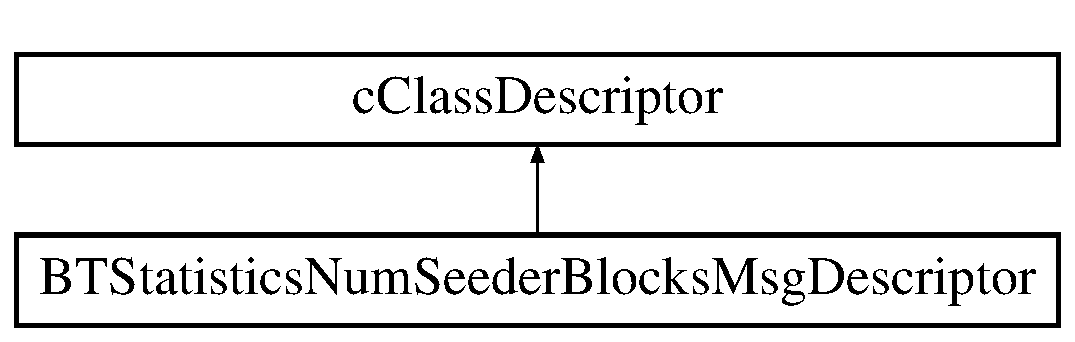
\includegraphics[height=2.000000cm]{classBTStatisticsNumSeederBlocksMsgDescriptor}
\end{center}
\end{figure}
\subsection*{Public Member Functions}
\begin{DoxyCompactItemize}
\item 
\hyperlink{classBTStatisticsNumSeederBlocksMsgDescriptor_af85eb363d05f9c88afbeca2c959865c3}{B\+T\+Statistics\+Num\+Seeder\+Blocks\+Msg\+Descriptor} ()
\item 
virtual \hyperlink{classBTStatisticsNumSeederBlocksMsgDescriptor_a8c1fecb22b154ec7e0505269af19c5ba}{$\sim$\+B\+T\+Statistics\+Num\+Seeder\+Blocks\+Msg\+Descriptor} ()
\item 
virtual bool \hyperlink{classBTStatisticsNumSeederBlocksMsgDescriptor_ad074d02067d275f08bd8e53180b12c94}{does\+Support} (c\+Object $\ast$obj) const 
\item 
virtual const char $\ast$ \hyperlink{classBTStatisticsNumSeederBlocksMsgDescriptor_a66a4a42b5791292bfb9263ea971fed95}{get\+Property} (const char $\ast$propertyname) const 
\item 
virtual int \hyperlink{classBTStatisticsNumSeederBlocksMsgDescriptor_a70257cf57d679793df1b079e5484e17b}{get\+Field\+Count} (void $\ast$object) const 
\item 
virtual const char $\ast$ \hyperlink{classBTStatisticsNumSeederBlocksMsgDescriptor_a80c7b028a3bafce0098df429b9551d87}{get\+Field\+Name} (void $\ast$object, int field) const 
\item 
virtual int \hyperlink{classBTStatisticsNumSeederBlocksMsgDescriptor_af848ccb483577f6953d1ebfe5c7950da}{find\+Field} (void $\ast$object, const char $\ast$field\+Name) const 
\item 
virtual unsigned int \hyperlink{classBTStatisticsNumSeederBlocksMsgDescriptor_a20e1005a6ab40b485b3f2b1eb8638dbd}{get\+Field\+Type\+Flags} (void $\ast$object, int field) const 
\item 
virtual const char $\ast$ \hyperlink{classBTStatisticsNumSeederBlocksMsgDescriptor_a6b10603bcde840217883848f4eb43baf}{get\+Field\+Type\+String} (void $\ast$object, int field) const 
\item 
virtual const char $\ast$ \hyperlink{classBTStatisticsNumSeederBlocksMsgDescriptor_a92f6318c1889c5cbd7d023c62daa92ee}{get\+Field\+Property} (void $\ast$object, int field, const char $\ast$propertyname) const 
\item 
virtual int \hyperlink{classBTStatisticsNumSeederBlocksMsgDescriptor_a63292c681585b96f92f9450dc0723f4f}{get\+Array\+Size} (void $\ast$object, int field) const 
\item 
virtual std\+::string \hyperlink{classBTStatisticsNumSeederBlocksMsgDescriptor_a4d890a6c0d3f079391438ca939fc3e6c}{get\+Field\+As\+String} (void $\ast$object, int field, int i) const 
\item 
virtual bool \hyperlink{classBTStatisticsNumSeederBlocksMsgDescriptor_a72356b2f10e62780019acf9b5ce39965}{set\+Field\+As\+String} (void $\ast$object, int field, int i, const char $\ast$value) const 
\item 
virtual const char $\ast$ \hyperlink{classBTStatisticsNumSeederBlocksMsgDescriptor_a6b58929d589860eca229ed3b559048d2}{get\+Field\+Struct\+Name} (void $\ast$object, int field) const 
\item 
virtual void $\ast$ \hyperlink{classBTStatisticsNumSeederBlocksMsgDescriptor_a046f0a78831652f6354ff9185996a778}{get\+Field\+Struct\+Pointer} (void $\ast$object, int field, int i) const 
\end{DoxyCompactItemize}


\subsection{Constructor \& Destructor Documentation}
\hypertarget{classBTStatisticsNumSeederBlocksMsgDescriptor_af85eb363d05f9c88afbeca2c959865c3}{}\index{B\+T\+Statistics\+Num\+Seeder\+Blocks\+Msg\+Descriptor@{B\+T\+Statistics\+Num\+Seeder\+Blocks\+Msg\+Descriptor}!B\+T\+Statistics\+Num\+Seeder\+Blocks\+Msg\+Descriptor@{B\+T\+Statistics\+Num\+Seeder\+Blocks\+Msg\+Descriptor}}
\index{B\+T\+Statistics\+Num\+Seeder\+Blocks\+Msg\+Descriptor@{B\+T\+Statistics\+Num\+Seeder\+Blocks\+Msg\+Descriptor}!B\+T\+Statistics\+Num\+Seeder\+Blocks\+Msg\+Descriptor@{B\+T\+Statistics\+Num\+Seeder\+Blocks\+Msg\+Descriptor}}
\subsubsection[{B\+T\+Statistics\+Num\+Seeder\+Blocks\+Msg\+Descriptor()}]{\setlength{\rightskip}{0pt plus 5cm}B\+T\+Statistics\+Num\+Seeder\+Blocks\+Msg\+Descriptor\+::\+B\+T\+Statistics\+Num\+Seeder\+Blocks\+Msg\+Descriptor (
\begin{DoxyParamCaption}
{}
\end{DoxyParamCaption}
)}\label{classBTStatisticsNumSeederBlocksMsgDescriptor_af85eb363d05f9c88afbeca2c959865c3}
\hypertarget{classBTStatisticsNumSeederBlocksMsgDescriptor_a8c1fecb22b154ec7e0505269af19c5ba}{}\index{B\+T\+Statistics\+Num\+Seeder\+Blocks\+Msg\+Descriptor@{B\+T\+Statistics\+Num\+Seeder\+Blocks\+Msg\+Descriptor}!````~B\+T\+Statistics\+Num\+Seeder\+Blocks\+Msg\+Descriptor@{$\sim$\+B\+T\+Statistics\+Num\+Seeder\+Blocks\+Msg\+Descriptor}}
\index{````~B\+T\+Statistics\+Num\+Seeder\+Blocks\+Msg\+Descriptor@{$\sim$\+B\+T\+Statistics\+Num\+Seeder\+Blocks\+Msg\+Descriptor}!B\+T\+Statistics\+Num\+Seeder\+Blocks\+Msg\+Descriptor@{B\+T\+Statistics\+Num\+Seeder\+Blocks\+Msg\+Descriptor}}
\subsubsection[{$\sim$\+B\+T\+Statistics\+Num\+Seeder\+Blocks\+Msg\+Descriptor()}]{\setlength{\rightskip}{0pt plus 5cm}B\+T\+Statistics\+Num\+Seeder\+Blocks\+Msg\+Descriptor\+::$\sim$\+B\+T\+Statistics\+Num\+Seeder\+Blocks\+Msg\+Descriptor (
\begin{DoxyParamCaption}
{}
\end{DoxyParamCaption}
)\hspace{0.3cm}{\ttfamily [virtual]}}\label{classBTStatisticsNumSeederBlocksMsgDescriptor_a8c1fecb22b154ec7e0505269af19c5ba}


\subsection{Member Function Documentation}
\hypertarget{classBTStatisticsNumSeederBlocksMsgDescriptor_ad074d02067d275f08bd8e53180b12c94}{}\index{B\+T\+Statistics\+Num\+Seeder\+Blocks\+Msg\+Descriptor@{B\+T\+Statistics\+Num\+Seeder\+Blocks\+Msg\+Descriptor}!does\+Support@{does\+Support}}
\index{does\+Support@{does\+Support}!B\+T\+Statistics\+Num\+Seeder\+Blocks\+Msg\+Descriptor@{B\+T\+Statistics\+Num\+Seeder\+Blocks\+Msg\+Descriptor}}
\subsubsection[{does\+Support(c\+Object $\ast$obj) const }]{\setlength{\rightskip}{0pt plus 5cm}bool B\+T\+Statistics\+Num\+Seeder\+Blocks\+Msg\+Descriptor\+::does\+Support (
\begin{DoxyParamCaption}
\item[{c\+Object $\ast$}]{obj}
\end{DoxyParamCaption}
) const\hspace{0.3cm}{\ttfamily [virtual]}}\label{classBTStatisticsNumSeederBlocksMsgDescriptor_ad074d02067d275f08bd8e53180b12c94}
\hypertarget{classBTStatisticsNumSeederBlocksMsgDescriptor_af848ccb483577f6953d1ebfe5c7950da}{}\index{B\+T\+Statistics\+Num\+Seeder\+Blocks\+Msg\+Descriptor@{B\+T\+Statistics\+Num\+Seeder\+Blocks\+Msg\+Descriptor}!find\+Field@{find\+Field}}
\index{find\+Field@{find\+Field}!B\+T\+Statistics\+Num\+Seeder\+Blocks\+Msg\+Descriptor@{B\+T\+Statistics\+Num\+Seeder\+Blocks\+Msg\+Descriptor}}
\subsubsection[{find\+Field(void $\ast$object, const char $\ast$field\+Name) const }]{\setlength{\rightskip}{0pt plus 5cm}int B\+T\+Statistics\+Num\+Seeder\+Blocks\+Msg\+Descriptor\+::find\+Field (
\begin{DoxyParamCaption}
\item[{void $\ast$}]{object, }
\item[{const char $\ast$}]{field\+Name}
\end{DoxyParamCaption}
) const\hspace{0.3cm}{\ttfamily [virtual]}}\label{classBTStatisticsNumSeederBlocksMsgDescriptor_af848ccb483577f6953d1ebfe5c7950da}
\hypertarget{classBTStatisticsNumSeederBlocksMsgDescriptor_a63292c681585b96f92f9450dc0723f4f}{}\index{B\+T\+Statistics\+Num\+Seeder\+Blocks\+Msg\+Descriptor@{B\+T\+Statistics\+Num\+Seeder\+Blocks\+Msg\+Descriptor}!get\+Array\+Size@{get\+Array\+Size}}
\index{get\+Array\+Size@{get\+Array\+Size}!B\+T\+Statistics\+Num\+Seeder\+Blocks\+Msg\+Descriptor@{B\+T\+Statistics\+Num\+Seeder\+Blocks\+Msg\+Descriptor}}
\subsubsection[{get\+Array\+Size(void $\ast$object, int field) const }]{\setlength{\rightskip}{0pt plus 5cm}int B\+T\+Statistics\+Num\+Seeder\+Blocks\+Msg\+Descriptor\+::get\+Array\+Size (
\begin{DoxyParamCaption}
\item[{void $\ast$}]{object, }
\item[{int}]{field}
\end{DoxyParamCaption}
) const\hspace{0.3cm}{\ttfamily [virtual]}}\label{classBTStatisticsNumSeederBlocksMsgDescriptor_a63292c681585b96f92f9450dc0723f4f}
\hypertarget{classBTStatisticsNumSeederBlocksMsgDescriptor_a4d890a6c0d3f079391438ca939fc3e6c}{}\index{B\+T\+Statistics\+Num\+Seeder\+Blocks\+Msg\+Descriptor@{B\+T\+Statistics\+Num\+Seeder\+Blocks\+Msg\+Descriptor}!get\+Field\+As\+String@{get\+Field\+As\+String}}
\index{get\+Field\+As\+String@{get\+Field\+As\+String}!B\+T\+Statistics\+Num\+Seeder\+Blocks\+Msg\+Descriptor@{B\+T\+Statistics\+Num\+Seeder\+Blocks\+Msg\+Descriptor}}
\subsubsection[{get\+Field\+As\+String(void $\ast$object, int field, int i) const }]{\setlength{\rightskip}{0pt plus 5cm}std\+::string B\+T\+Statistics\+Num\+Seeder\+Blocks\+Msg\+Descriptor\+::get\+Field\+As\+String (
\begin{DoxyParamCaption}
\item[{void $\ast$}]{object, }
\item[{int}]{field, }
\item[{int}]{i}
\end{DoxyParamCaption}
) const\hspace{0.3cm}{\ttfamily [virtual]}}\label{classBTStatisticsNumSeederBlocksMsgDescriptor_a4d890a6c0d3f079391438ca939fc3e6c}
\hypertarget{classBTStatisticsNumSeederBlocksMsgDescriptor_a70257cf57d679793df1b079e5484e17b}{}\index{B\+T\+Statistics\+Num\+Seeder\+Blocks\+Msg\+Descriptor@{B\+T\+Statistics\+Num\+Seeder\+Blocks\+Msg\+Descriptor}!get\+Field\+Count@{get\+Field\+Count}}
\index{get\+Field\+Count@{get\+Field\+Count}!B\+T\+Statistics\+Num\+Seeder\+Blocks\+Msg\+Descriptor@{B\+T\+Statistics\+Num\+Seeder\+Blocks\+Msg\+Descriptor}}
\subsubsection[{get\+Field\+Count(void $\ast$object) const }]{\setlength{\rightskip}{0pt plus 5cm}int B\+T\+Statistics\+Num\+Seeder\+Blocks\+Msg\+Descriptor\+::get\+Field\+Count (
\begin{DoxyParamCaption}
\item[{void $\ast$}]{object}
\end{DoxyParamCaption}
) const\hspace{0.3cm}{\ttfamily [virtual]}}\label{classBTStatisticsNumSeederBlocksMsgDescriptor_a70257cf57d679793df1b079e5484e17b}
\hypertarget{classBTStatisticsNumSeederBlocksMsgDescriptor_a80c7b028a3bafce0098df429b9551d87}{}\index{B\+T\+Statistics\+Num\+Seeder\+Blocks\+Msg\+Descriptor@{B\+T\+Statistics\+Num\+Seeder\+Blocks\+Msg\+Descriptor}!get\+Field\+Name@{get\+Field\+Name}}
\index{get\+Field\+Name@{get\+Field\+Name}!B\+T\+Statistics\+Num\+Seeder\+Blocks\+Msg\+Descriptor@{B\+T\+Statistics\+Num\+Seeder\+Blocks\+Msg\+Descriptor}}
\subsubsection[{get\+Field\+Name(void $\ast$object, int field) const }]{\setlength{\rightskip}{0pt plus 5cm}const char $\ast$ B\+T\+Statistics\+Num\+Seeder\+Blocks\+Msg\+Descriptor\+::get\+Field\+Name (
\begin{DoxyParamCaption}
\item[{void $\ast$}]{object, }
\item[{int}]{field}
\end{DoxyParamCaption}
) const\hspace{0.3cm}{\ttfamily [virtual]}}\label{classBTStatisticsNumSeederBlocksMsgDescriptor_a80c7b028a3bafce0098df429b9551d87}
\hypertarget{classBTStatisticsNumSeederBlocksMsgDescriptor_a92f6318c1889c5cbd7d023c62daa92ee}{}\index{B\+T\+Statistics\+Num\+Seeder\+Blocks\+Msg\+Descriptor@{B\+T\+Statistics\+Num\+Seeder\+Blocks\+Msg\+Descriptor}!get\+Field\+Property@{get\+Field\+Property}}
\index{get\+Field\+Property@{get\+Field\+Property}!B\+T\+Statistics\+Num\+Seeder\+Blocks\+Msg\+Descriptor@{B\+T\+Statistics\+Num\+Seeder\+Blocks\+Msg\+Descriptor}}
\subsubsection[{get\+Field\+Property(void $\ast$object, int field, const char $\ast$propertyname) const }]{\setlength{\rightskip}{0pt plus 5cm}const char $\ast$ B\+T\+Statistics\+Num\+Seeder\+Blocks\+Msg\+Descriptor\+::get\+Field\+Property (
\begin{DoxyParamCaption}
\item[{void $\ast$}]{object, }
\item[{int}]{field, }
\item[{const char $\ast$}]{propertyname}
\end{DoxyParamCaption}
) const\hspace{0.3cm}{\ttfamily [virtual]}}\label{classBTStatisticsNumSeederBlocksMsgDescriptor_a92f6318c1889c5cbd7d023c62daa92ee}
\hypertarget{classBTStatisticsNumSeederBlocksMsgDescriptor_a6b58929d589860eca229ed3b559048d2}{}\index{B\+T\+Statistics\+Num\+Seeder\+Blocks\+Msg\+Descriptor@{B\+T\+Statistics\+Num\+Seeder\+Blocks\+Msg\+Descriptor}!get\+Field\+Struct\+Name@{get\+Field\+Struct\+Name}}
\index{get\+Field\+Struct\+Name@{get\+Field\+Struct\+Name}!B\+T\+Statistics\+Num\+Seeder\+Blocks\+Msg\+Descriptor@{B\+T\+Statistics\+Num\+Seeder\+Blocks\+Msg\+Descriptor}}
\subsubsection[{get\+Field\+Struct\+Name(void $\ast$object, int field) const }]{\setlength{\rightskip}{0pt plus 5cm}const char $\ast$ B\+T\+Statistics\+Num\+Seeder\+Blocks\+Msg\+Descriptor\+::get\+Field\+Struct\+Name (
\begin{DoxyParamCaption}
\item[{void $\ast$}]{object, }
\item[{int}]{field}
\end{DoxyParamCaption}
) const\hspace{0.3cm}{\ttfamily [virtual]}}\label{classBTStatisticsNumSeederBlocksMsgDescriptor_a6b58929d589860eca229ed3b559048d2}
\hypertarget{classBTStatisticsNumSeederBlocksMsgDescriptor_a046f0a78831652f6354ff9185996a778}{}\index{B\+T\+Statistics\+Num\+Seeder\+Blocks\+Msg\+Descriptor@{B\+T\+Statistics\+Num\+Seeder\+Blocks\+Msg\+Descriptor}!get\+Field\+Struct\+Pointer@{get\+Field\+Struct\+Pointer}}
\index{get\+Field\+Struct\+Pointer@{get\+Field\+Struct\+Pointer}!B\+T\+Statistics\+Num\+Seeder\+Blocks\+Msg\+Descriptor@{B\+T\+Statistics\+Num\+Seeder\+Blocks\+Msg\+Descriptor}}
\subsubsection[{get\+Field\+Struct\+Pointer(void $\ast$object, int field, int i) const }]{\setlength{\rightskip}{0pt plus 5cm}void $\ast$ B\+T\+Statistics\+Num\+Seeder\+Blocks\+Msg\+Descriptor\+::get\+Field\+Struct\+Pointer (
\begin{DoxyParamCaption}
\item[{void $\ast$}]{object, }
\item[{int}]{field, }
\item[{int}]{i}
\end{DoxyParamCaption}
) const\hspace{0.3cm}{\ttfamily [virtual]}}\label{classBTStatisticsNumSeederBlocksMsgDescriptor_a046f0a78831652f6354ff9185996a778}
\hypertarget{classBTStatisticsNumSeederBlocksMsgDescriptor_a20e1005a6ab40b485b3f2b1eb8638dbd}{}\index{B\+T\+Statistics\+Num\+Seeder\+Blocks\+Msg\+Descriptor@{B\+T\+Statistics\+Num\+Seeder\+Blocks\+Msg\+Descriptor}!get\+Field\+Type\+Flags@{get\+Field\+Type\+Flags}}
\index{get\+Field\+Type\+Flags@{get\+Field\+Type\+Flags}!B\+T\+Statistics\+Num\+Seeder\+Blocks\+Msg\+Descriptor@{B\+T\+Statistics\+Num\+Seeder\+Blocks\+Msg\+Descriptor}}
\subsubsection[{get\+Field\+Type\+Flags(void $\ast$object, int field) const }]{\setlength{\rightskip}{0pt plus 5cm}unsigned int B\+T\+Statistics\+Num\+Seeder\+Blocks\+Msg\+Descriptor\+::get\+Field\+Type\+Flags (
\begin{DoxyParamCaption}
\item[{void $\ast$}]{object, }
\item[{int}]{field}
\end{DoxyParamCaption}
) const\hspace{0.3cm}{\ttfamily [virtual]}}\label{classBTStatisticsNumSeederBlocksMsgDescriptor_a20e1005a6ab40b485b3f2b1eb8638dbd}
\hypertarget{classBTStatisticsNumSeederBlocksMsgDescriptor_a6b10603bcde840217883848f4eb43baf}{}\index{B\+T\+Statistics\+Num\+Seeder\+Blocks\+Msg\+Descriptor@{B\+T\+Statistics\+Num\+Seeder\+Blocks\+Msg\+Descriptor}!get\+Field\+Type\+String@{get\+Field\+Type\+String}}
\index{get\+Field\+Type\+String@{get\+Field\+Type\+String}!B\+T\+Statistics\+Num\+Seeder\+Blocks\+Msg\+Descriptor@{B\+T\+Statistics\+Num\+Seeder\+Blocks\+Msg\+Descriptor}}
\subsubsection[{get\+Field\+Type\+String(void $\ast$object, int field) const }]{\setlength{\rightskip}{0pt plus 5cm}const char $\ast$ B\+T\+Statistics\+Num\+Seeder\+Blocks\+Msg\+Descriptor\+::get\+Field\+Type\+String (
\begin{DoxyParamCaption}
\item[{void $\ast$}]{object, }
\item[{int}]{field}
\end{DoxyParamCaption}
) const\hspace{0.3cm}{\ttfamily [virtual]}}\label{classBTStatisticsNumSeederBlocksMsgDescriptor_a6b10603bcde840217883848f4eb43baf}
\hypertarget{classBTStatisticsNumSeederBlocksMsgDescriptor_a66a4a42b5791292bfb9263ea971fed95}{}\index{B\+T\+Statistics\+Num\+Seeder\+Blocks\+Msg\+Descriptor@{B\+T\+Statistics\+Num\+Seeder\+Blocks\+Msg\+Descriptor}!get\+Property@{get\+Property}}
\index{get\+Property@{get\+Property}!B\+T\+Statistics\+Num\+Seeder\+Blocks\+Msg\+Descriptor@{B\+T\+Statistics\+Num\+Seeder\+Blocks\+Msg\+Descriptor}}
\subsubsection[{get\+Property(const char $\ast$propertyname) const }]{\setlength{\rightskip}{0pt plus 5cm}const char $\ast$ B\+T\+Statistics\+Num\+Seeder\+Blocks\+Msg\+Descriptor\+::get\+Property (
\begin{DoxyParamCaption}
\item[{const char $\ast$}]{propertyname}
\end{DoxyParamCaption}
) const\hspace{0.3cm}{\ttfamily [virtual]}}\label{classBTStatisticsNumSeederBlocksMsgDescriptor_a66a4a42b5791292bfb9263ea971fed95}
\hypertarget{classBTStatisticsNumSeederBlocksMsgDescriptor_a72356b2f10e62780019acf9b5ce39965}{}\index{B\+T\+Statistics\+Num\+Seeder\+Blocks\+Msg\+Descriptor@{B\+T\+Statistics\+Num\+Seeder\+Blocks\+Msg\+Descriptor}!set\+Field\+As\+String@{set\+Field\+As\+String}}
\index{set\+Field\+As\+String@{set\+Field\+As\+String}!B\+T\+Statistics\+Num\+Seeder\+Blocks\+Msg\+Descriptor@{B\+T\+Statistics\+Num\+Seeder\+Blocks\+Msg\+Descriptor}}
\subsubsection[{set\+Field\+As\+String(void $\ast$object, int field, int i, const char $\ast$value) const }]{\setlength{\rightskip}{0pt plus 5cm}bool B\+T\+Statistics\+Num\+Seeder\+Blocks\+Msg\+Descriptor\+::set\+Field\+As\+String (
\begin{DoxyParamCaption}
\item[{void $\ast$}]{object, }
\item[{int}]{field, }
\item[{int}]{i, }
\item[{const char $\ast$}]{value}
\end{DoxyParamCaption}
) const\hspace{0.3cm}{\ttfamily [virtual]}}\label{classBTStatisticsNumSeederBlocksMsgDescriptor_a72356b2f10e62780019acf9b5ce39965}


The documentation for this class was generated from the following file\+:\begin{DoxyCompactItemize}
\item 
\hyperlink{BTStatisticsMsg__m_8cc}{B\+T\+Statistics\+Msg\+\_\+m.\+cc}\end{DoxyCompactItemize}

\hypertarget{classBTTrackerBase}{}\section{B\+T\+Tracker\+Base Class Reference}
\label{classBTTrackerBase}\index{B\+T\+Tracker\+Base@{B\+T\+Tracker\+Base}}


{\ttfamily \#include $<$B\+T\+Tracker\+Base.\+h$>$}

Inheritance diagram for B\+T\+Tracker\+Base\+:\begin{figure}[H]
\begin{center}
\leavevmode
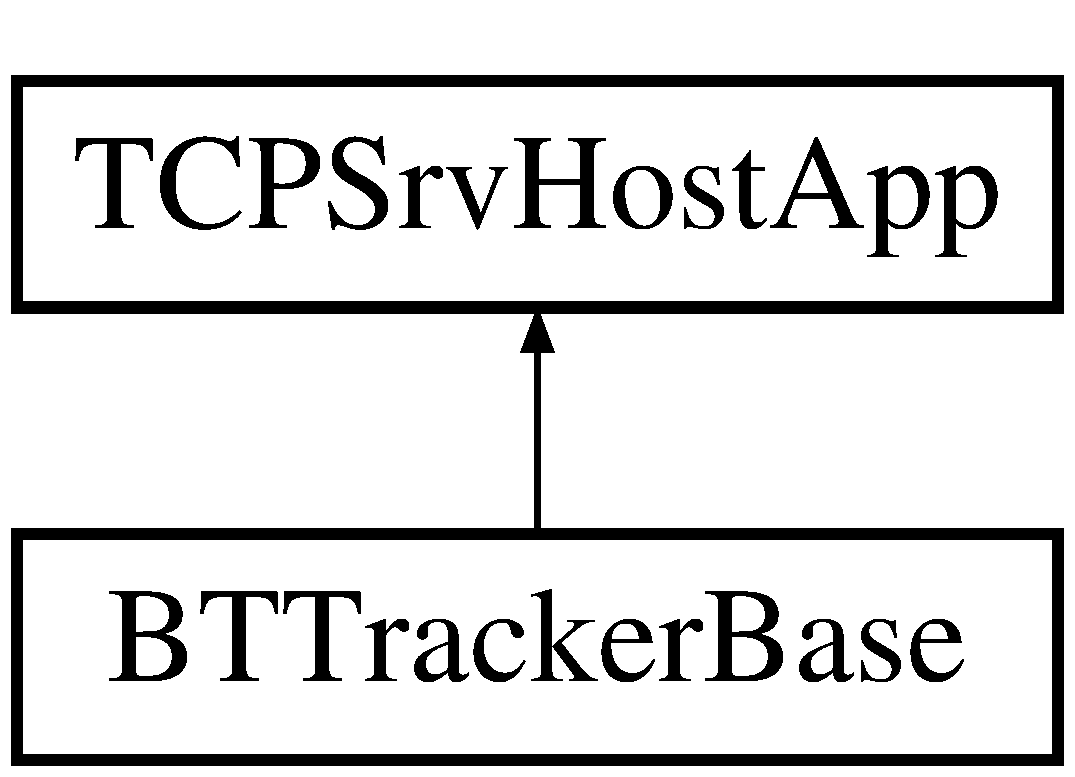
\includegraphics[height=2.000000cm]{classBTTrackerBase}
\end{center}
\end{figure}
\subsection*{Public Member Functions}
\begin{DoxyCompactItemize}
\item 
\hyperlink{classBTTrackerBase_a05a7a0e4b4514e39d25dcf7d34bc254f}{B\+T\+Tracker\+Base} ()
\item 
virtual \hyperlink{classBTTrackerBase_a8b324ddad0dae22cccb338ce183e12b4}{$\sim$\+B\+T\+Tracker\+Base} ()
\item 
const string \& \hyperlink{classBTTrackerBase_ad3744373908aaae2c9f88a989f711164}{info\+Hash} () const 
\item 
void \hyperlink{classBTTrackerBase_aa205b2d356794b9414429b6a9bced23b}{set\+Info\+Hash} (const string \&)
\item 
const string \& \hyperlink{classBTTrackerBase_a3892d03da0e26565e6e7e2f813026d7e}{tracker\+Id} () const 
\item 
void \hyperlink{classBTTrackerBase_ab8a18224107ed0910dc0bd1638e6c79e}{set\+Tracker\+Id} (const string \&)
\item 
bool \hyperlink{classBTTrackerBase_a30633c30f74aa526f500587df8f449be}{always\+Send\+Tracker\+Id} () const 
\item 
void \hyperlink{classBTTrackerBase_ad0894e8d363b622b5bb499d13fb62669}{set\+Always\+Send\+Tracker\+Id} (bool)
\item 
bool \hyperlink{classBTTrackerBase_a65a57779fc1a54b53d8730e645246588}{compact\+Support} () const 
\item 
void \hyperlink{classBTTrackerBase_adfebd2b9c4efb1c140bf89a926aa67f8}{set\+Compact\+Support} (bool)
\item 
size\+\_\+t \hyperlink{classBTTrackerBase_a0c341d939c255dea96f2fd9e84fe4dc9}{max\+Peers\+In\+Reply} () const 
\item 
void \hyperlink{classBTTrackerBase_aefc9c49a92f7283de65369d4cfe1236d}{set\+Max\+Peers\+In\+Reply} (size\+\_\+t)
\item 
size\+\_\+t \hyperlink{classBTTrackerBase_a6485fae29881927c04d7271ac28f01eb}{announce\+Interval} () const 
\item 
void \hyperlink{classBTTrackerBase_a05438a148023a31cd72d352e381af208}{set\+Announce\+Interval} (size\+\_\+t)
\item 
size\+\_\+t \hyperlink{classBTTrackerBase_a46737e1276c56c9dc83264cc8cde501a}{cleanup\+Interval} () const 
\item 
void \hyperlink{classBTTrackerBase_ae455bf93bf9c4aac9346e28132358767}{set\+Cleanup\+Interval} (size\+\_\+t)
\item 
size\+\_\+t \hyperlink{classBTTrackerBase_aa25cbbeee60a86a81bd862d74bb098b5}{session\+Timeout} () const 
\item 
void \hyperlink{classBTTrackerBase_a978f8dc10a807b37eac2615f8a6b6a36}{set\+Session\+Timeout} (size\+\_\+t)
\item 
c\+Array \& \hyperlink{classBTTrackerBase_ab5dd962e8b31d9da764cac4339f88bb6}{peers} ()
\item 
int \hyperlink{classBTTrackerBase_aee3f129e66a6690df7e6e3279599f171}{contains} (\hyperlink{classBTTrackerStructBase}{B\+T\+Tracker\+Struct\+Base} $\ast$) const 
\item 
size\+\_\+t \hyperlink{classBTTrackerBase_ae5c78b500fcbcf7a4881d3f584a3027d}{seeds} () const 
\item 
void \hyperlink{classBTTrackerBase_af9b9f0ed01cf67b1e464402f6f884f42}{set\+Seeds} (size\+\_\+t)
\item 
size\+\_\+t \hyperlink{classBTTrackerBase_aabbe120067d9081485e90a4e71e675b7}{peers\+Num} () const 
\item 
void \hyperlink{classBTTrackerBase_aee0793e4cabbd2f61104587c4aff5a31}{set\+Peers\+Num} (size\+\_\+t)
\item 
void \hyperlink{classBTTrackerBase_ad1b9190f3117918ce2404f6fae5af26a}{clean\+Up\+Peers} ()
\item 
void \hyperlink{classBTTrackerBase_ae2ccfb420d08172f2ed5b544c9067fd5}{clean\+Remove\+Peer} (\hyperlink{classBTTrackerStructBase}{B\+T\+Tracker\+Struct\+Base} $\ast$)
\item 
void \hyperlink{classBTTrackerBase_ab1600e226ac13ecfbf9993e50cd8f1b2}{clean\+Remove\+Peer} (int)
\end{DoxyCompactItemize}
\subsection*{Protected Member Functions}
\begin{DoxyCompactItemize}
\item 
virtual void \hyperlink{classBTTrackerBase_a0bc53255febc095ae8ac4b5efc53d193}{initialize} ()
\item 
virtual void \hyperlink{classBTTrackerBase_a88120a6f9fb7e0ddbc3b4c794b842572}{handle\+Message} (c\+Message $\ast$)
\end{DoxyCompactItemize}
\subsection*{Protected Attributes}
\begin{DoxyCompactItemize}
\item 
string \hyperlink{classBTTrackerBase_a6164025eda001522313b120b94cf1049}{info\+Hash\+\_\+var}
\item 
string \hyperlink{classBTTrackerBase_adf43f3c801c6904772843b85bc6d2c13}{tracker\+Id\+\_\+var}
\item 
bool \hyperlink{classBTTrackerBase_aa627eb44986bdbbbd1afa58900c2d0f7}{always\+Send\+Tracker\+Id\+\_\+var}
\item 
bool \hyperlink{classBTTrackerBase_aeb6d8973fe084f768e436a8ce5da35d7}{compact\+Support\+\_\+var}
\item 
size\+\_\+t \hyperlink{classBTTrackerBase_ad4b07408463db605eca2706185353107}{max\+Peers\+In\+Reply\+\_\+var}
\item 
size\+\_\+t \hyperlink{classBTTrackerBase_a878a13b70d17fa3e4af1d9548e15c381}{announce\+Interval\+\_\+var}
\item 
size\+\_\+t \hyperlink{classBTTrackerBase_a7b008007cf154ef938d38898b4d25d7c}{cleanup\+Interval\+\_\+var}
\item 
size\+\_\+t \hyperlink{classBTTrackerBase_a1ced4f437ab0e81e1904c17c4e7b3f02}{session\+Timeout\+\_\+var}
\item 
c\+Array \hyperlink{classBTTrackerBase_a7e935c84f601dc0f7f7c51fd7b9bc8bd}{peers\+\_\+var}
\item 
size\+\_\+t \hyperlink{classBTTrackerBase_a4741f78f0b5f6393f6b2634f0fd77109}{seeds\+\_\+var}
\item 
size\+\_\+t \hyperlink{classBTTrackerBase_aa13e59ee55a6ee18af0828fa9e54a01d}{peers\+Num\+\_\+var}
\item 
c\+Message $\ast$ \hyperlink{classBTTrackerBase_a12ea7d9b9e19b425289d8d3197cebae6}{clean}
\item 
size\+\_\+t \hyperlink{classBTTrackerBase_a951142be9da0bbc37937e0f9199af38f}{curr\+Clean\+\_\+exit\+\_\+var}
\end{DoxyCompactItemize}


\subsection{Detailed Description}
Bit\+Torrent protocol. Implements a threaded tracker as described at \href{http://wiki.theory.org/BitTorrentSpecification}{\tt http\+://wiki.\+theory.\+org/\+Bit\+Torrent\+Specification} 

\subsection{Constructor \& Destructor Documentation}
\hypertarget{classBTTrackerBase_a05a7a0e4b4514e39d25dcf7d34bc254f}{}\index{B\+T\+Tracker\+Base@{B\+T\+Tracker\+Base}!B\+T\+Tracker\+Base@{B\+T\+Tracker\+Base}}
\index{B\+T\+Tracker\+Base@{B\+T\+Tracker\+Base}!B\+T\+Tracker\+Base@{B\+T\+Tracker\+Base}}
\subsubsection[{B\+T\+Tracker\+Base()}]{\setlength{\rightskip}{0pt plus 5cm}B\+T\+Tracker\+Base\+::\+B\+T\+Tracker\+Base (
\begin{DoxyParamCaption}
{}
\end{DoxyParamCaption}
)}\label{classBTTrackerBase_a05a7a0e4b4514e39d25dcf7d34bc254f}
Constructor. \hypertarget{classBTTrackerBase_a8b324ddad0dae22cccb338ce183e12b4}{}\index{B\+T\+Tracker\+Base@{B\+T\+Tracker\+Base}!````~B\+T\+Tracker\+Base@{$\sim$\+B\+T\+Tracker\+Base}}
\index{````~B\+T\+Tracker\+Base@{$\sim$\+B\+T\+Tracker\+Base}!B\+T\+Tracker\+Base@{B\+T\+Tracker\+Base}}
\subsubsection[{$\sim$\+B\+T\+Tracker\+Base()}]{\setlength{\rightskip}{0pt plus 5cm}B\+T\+Tracker\+Base\+::$\sim$\+B\+T\+Tracker\+Base (
\begin{DoxyParamCaption}
{}
\end{DoxyParamCaption}
)\hspace{0.3cm}{\ttfamily [virtual]}}\label{classBTTrackerBase_a8b324ddad0dae22cccb338ce183e12b4}
Destructor. 

\subsection{Member Function Documentation}
\hypertarget{classBTTrackerBase_a30633c30f74aa526f500587df8f449be}{}\index{B\+T\+Tracker\+Base@{B\+T\+Tracker\+Base}!always\+Send\+Tracker\+Id@{always\+Send\+Tracker\+Id}}
\index{always\+Send\+Tracker\+Id@{always\+Send\+Tracker\+Id}!B\+T\+Tracker\+Base@{B\+T\+Tracker\+Base}}
\subsubsection[{always\+Send\+Tracker\+Id() const }]{\setlength{\rightskip}{0pt plus 5cm}bool B\+T\+Tracker\+Base\+::always\+Send\+Tracker\+Id (
\begin{DoxyParamCaption}
{}
\end{DoxyParamCaption}
) const}\label{classBTTrackerBase_a30633c30f74aa526f500587df8f449be}
Get the always\+Send\+Tracker\+Id flag. If the flag is true the tracker id will be returned in every response. If the flag is set to false the tracker id will be returned to the client only in the first response. \hypertarget{classBTTrackerBase_a6485fae29881927c04d7271ac28f01eb}{}\index{B\+T\+Tracker\+Base@{B\+T\+Tracker\+Base}!announce\+Interval@{announce\+Interval}}
\index{announce\+Interval@{announce\+Interval}!B\+T\+Tracker\+Base@{B\+T\+Tracker\+Base}}
\subsubsection[{announce\+Interval() const }]{\setlength{\rightskip}{0pt plus 5cm}size\+\_\+t B\+T\+Tracker\+Base\+::announce\+Interval (
\begin{DoxyParamCaption}
{}
\end{DoxyParamCaption}
) const}\label{classBTTrackerBase_a6485fae29881927c04d7271ac28f01eb}
\hypertarget{classBTTrackerBase_ae2ccfb420d08172f2ed5b544c9067fd5}{}\index{B\+T\+Tracker\+Base@{B\+T\+Tracker\+Base}!clean\+Remove\+Peer@{clean\+Remove\+Peer}}
\index{clean\+Remove\+Peer@{clean\+Remove\+Peer}!B\+T\+Tracker\+Base@{B\+T\+Tracker\+Base}}
\subsubsection[{clean\+Remove\+Peer(\+B\+T\+Tracker\+Struct\+Base $\ast$)}]{\setlength{\rightskip}{0pt plus 5cm}void B\+T\+Tracker\+Base\+::clean\+Remove\+Peer (
\begin{DoxyParamCaption}
\item[{{\bf B\+T\+Tracker\+Struct\+Base} $\ast$}]{peer}
\end{DoxyParamCaption}
)}\label{classBTTrackerBase_ae2ccfb420d08172f2ed5b544c9067fd5}
Remove a peer from the peer set ensuring memory deallocation. \hypertarget{classBTTrackerBase_ab1600e226ac13ecfbf9993e50cd8f1b2}{}\index{B\+T\+Tracker\+Base@{B\+T\+Tracker\+Base}!clean\+Remove\+Peer@{clean\+Remove\+Peer}}
\index{clean\+Remove\+Peer@{clean\+Remove\+Peer}!B\+T\+Tracker\+Base@{B\+T\+Tracker\+Base}}
\subsubsection[{clean\+Remove\+Peer(int)}]{\setlength{\rightskip}{0pt plus 5cm}void B\+T\+Tracker\+Base\+::clean\+Remove\+Peer (
\begin{DoxyParamCaption}
\item[{int}]{index}
\end{DoxyParamCaption}
)}\label{classBTTrackerBase_ab1600e226ac13ecfbf9993e50cd8f1b2}
Remove a peer from the peer set ensuring memory deallocation. \hypertarget{classBTTrackerBase_a46737e1276c56c9dc83264cc8cde501a}{}\index{B\+T\+Tracker\+Base@{B\+T\+Tracker\+Base}!cleanup\+Interval@{cleanup\+Interval}}
\index{cleanup\+Interval@{cleanup\+Interval}!B\+T\+Tracker\+Base@{B\+T\+Tracker\+Base}}
\subsubsection[{cleanup\+Interval() const }]{\setlength{\rightskip}{0pt plus 5cm}size\+\_\+t B\+T\+Tracker\+Base\+::cleanup\+Interval (
\begin{DoxyParamCaption}
{}
\end{DoxyParamCaption}
) const}\label{classBTTrackerBase_a46737e1276c56c9dc83264cc8cde501a}
Get the announce interval (in seconds). \hypertarget{classBTTrackerBase_ad1b9190f3117918ce2404f6fae5af26a}{}\index{B\+T\+Tracker\+Base@{B\+T\+Tracker\+Base}!clean\+Up\+Peers@{clean\+Up\+Peers}}
\index{clean\+Up\+Peers@{clean\+Up\+Peers}!B\+T\+Tracker\+Base@{B\+T\+Tracker\+Base}}
\subsubsection[{clean\+Up\+Peers()}]{\setlength{\rightskip}{0pt plus 5cm}void B\+T\+Tracker\+Base\+::clean\+Up\+Peers (
\begin{DoxyParamCaption}
{}
\end{DoxyParamCaption}
)}\label{classBTTrackerBase_ad1b9190f3117918ce2404f6fae5af26a}
Deallocating memory used for the peer set. \hypertarget{classBTTrackerBase_a65a57779fc1a54b53d8730e645246588}{}\index{B\+T\+Tracker\+Base@{B\+T\+Tracker\+Base}!compact\+Support@{compact\+Support}}
\index{compact\+Support@{compact\+Support}!B\+T\+Tracker\+Base@{B\+T\+Tracker\+Base}}
\subsubsection[{compact\+Support() const }]{\setlength{\rightskip}{0pt plus 5cm}bool B\+T\+Tracker\+Base\+::compact\+Support (
\begin{DoxyParamCaption}
{}
\end{DoxyParamCaption}
) const}\label{classBTTrackerBase_a65a57779fc1a54b53d8730e645246588}
Get the compact\+Support flag. Support for compact responses or not. \hypertarget{classBTTrackerBase_aee3f129e66a6690df7e6e3279599f171}{}\index{B\+T\+Tracker\+Base@{B\+T\+Tracker\+Base}!contains@{contains}}
\index{contains@{contains}!B\+T\+Tracker\+Base@{B\+T\+Tracker\+Base}}
\subsubsection[{contains(\+B\+T\+Tracker\+Struct\+Base $\ast$) const }]{\setlength{\rightskip}{0pt plus 5cm}int B\+T\+Tracker\+Base\+::contains (
\begin{DoxyParamCaption}
\item[{{\bf B\+T\+Tracker\+Struct\+Base} $\ast$}]{obj}
\end{DoxyParamCaption}
) const}\label{classBTTrackerBase_aee3f129e66a6690df7e6e3279599f171}
Returns the position of obj inside the peers container (if it is contained) or -\/1 if obj is not found.

This lame method was inserted because the find() method of the c\+Array class is so stupid that does not use the overloaded == operator. \hypertarget{classBTTrackerBase_a88120a6f9fb7e0ddbc3b4c794b842572}{}\index{B\+T\+Tracker\+Base@{B\+T\+Tracker\+Base}!handle\+Message@{handle\+Message}}
\index{handle\+Message@{handle\+Message}!B\+T\+Tracker\+Base@{B\+T\+Tracker\+Base}}
\subsubsection[{handle\+Message(c\+Message $\ast$)}]{\setlength{\rightskip}{0pt plus 5cm}void B\+T\+Tracker\+Base\+::handle\+Message (
\begin{DoxyParamCaption}
\item[{c\+Message $\ast$}]{msg}
\end{DoxyParamCaption}
)\hspace{0.3cm}{\ttfamily [protected]}, {\ttfamily [virtual]}}\label{classBTTrackerBase_a88120a6f9fb7e0ddbc3b4c794b842572}
Called each time a new message is received. \hypertarget{classBTTrackerBase_ad3744373908aaae2c9f88a989f711164}{}\index{B\+T\+Tracker\+Base@{B\+T\+Tracker\+Base}!info\+Hash@{info\+Hash}}
\index{info\+Hash@{info\+Hash}!B\+T\+Tracker\+Base@{B\+T\+Tracker\+Base}}
\subsubsection[{info\+Hash() const }]{\setlength{\rightskip}{0pt plus 5cm}const string \& B\+T\+Tracker\+Base\+::info\+Hash (
\begin{DoxyParamCaption}
{}
\end{DoxyParamCaption}
) const}\label{classBTTrackerBase_ad3744373908aaae2c9f88a989f711164}
Get the info hash of tracker. This is the info hash of the .torrent file which the tracker monitors. \hypertarget{classBTTrackerBase_a0bc53255febc095ae8ac4b5efc53d193}{}\index{B\+T\+Tracker\+Base@{B\+T\+Tracker\+Base}!initialize@{initialize}}
\index{initialize@{initialize}!B\+T\+Tracker\+Base@{B\+T\+Tracker\+Base}}
\subsubsection[{initialize()}]{\setlength{\rightskip}{0pt plus 5cm}void B\+T\+Tracker\+Base\+::initialize (
\begin{DoxyParamCaption}
{}
\end{DoxyParamCaption}
)\hspace{0.3cm}{\ttfamily [protected]}, {\ttfamily [virtual]}}\label{classBTTrackerBase_a0bc53255febc095ae8ac4b5efc53d193}
Called after the module creation. \hypertarget{classBTTrackerBase_a0c341d939c255dea96f2fd9e84fe4dc9}{}\index{B\+T\+Tracker\+Base@{B\+T\+Tracker\+Base}!max\+Peers\+In\+Reply@{max\+Peers\+In\+Reply}}
\index{max\+Peers\+In\+Reply@{max\+Peers\+In\+Reply}!B\+T\+Tracker\+Base@{B\+T\+Tracker\+Base}}
\subsubsection[{max\+Peers\+In\+Reply() const }]{\setlength{\rightskip}{0pt plus 5cm}size\+\_\+t B\+T\+Tracker\+Base\+::max\+Peers\+In\+Reply (
\begin{DoxyParamCaption}
{}
\end{DoxyParamCaption}
) const}\label{classBTTrackerBase_a0c341d939c255dea96f2fd9e84fe4dc9}
\hypertarget{classBTTrackerBase_ab5dd962e8b31d9da764cac4339f88bb6}{}\index{B\+T\+Tracker\+Base@{B\+T\+Tracker\+Base}!peers@{peers}}
\index{peers@{peers}!B\+T\+Tracker\+Base@{B\+T\+Tracker\+Base}}
\subsubsection[{peers()}]{\setlength{\rightskip}{0pt plus 5cm}c\+Array \& B\+T\+Tracker\+Base\+::peers (
\begin{DoxyParamCaption}
{}
\end{DoxyParamCaption}
)}\label{classBTTrackerBase_ab5dd962e8b31d9da764cac4339f88bb6}
Get the peers container. \hypertarget{classBTTrackerBase_aabbe120067d9081485e90a4e71e675b7}{}\index{B\+T\+Tracker\+Base@{B\+T\+Tracker\+Base}!peers\+Num@{peers\+Num}}
\index{peers\+Num@{peers\+Num}!B\+T\+Tracker\+Base@{B\+T\+Tracker\+Base}}
\subsubsection[{peers\+Num() const }]{\setlength{\rightskip}{0pt plus 5cm}size\+\_\+t B\+T\+Tracker\+Base\+::peers\+Num (
\begin{DoxyParamCaption}
{}
\end{DoxyParamCaption}
) const}\label{classBTTrackerBase_aabbe120067d9081485e90a4e71e675b7}
Get the peers count. \hypertarget{classBTTrackerBase_ae5c78b500fcbcf7a4881d3f584a3027d}{}\index{B\+T\+Tracker\+Base@{B\+T\+Tracker\+Base}!seeds@{seeds}}
\index{seeds@{seeds}!B\+T\+Tracker\+Base@{B\+T\+Tracker\+Base}}
\subsubsection[{seeds() const }]{\setlength{\rightskip}{0pt plus 5cm}size\+\_\+t B\+T\+Tracker\+Base\+::seeds (
\begin{DoxyParamCaption}
{}
\end{DoxyParamCaption}
) const}\label{classBTTrackerBase_ae5c78b500fcbcf7a4881d3f584a3027d}
Get the seeds count. \hypertarget{classBTTrackerBase_aa25cbbeee60a86a81bd862d74bb098b5}{}\index{B\+T\+Tracker\+Base@{B\+T\+Tracker\+Base}!session\+Timeout@{session\+Timeout}}
\index{session\+Timeout@{session\+Timeout}!B\+T\+Tracker\+Base@{B\+T\+Tracker\+Base}}
\subsubsection[{session\+Timeout() const }]{\setlength{\rightskip}{0pt plus 5cm}size\+\_\+t B\+T\+Tracker\+Base\+::session\+Timeout (
\begin{DoxyParamCaption}
{}
\end{DoxyParamCaption}
) const}\label{classBTTrackerBase_aa25cbbeee60a86a81bd862d74bb098b5}
Get the cleanup interval (in seconds). \hypertarget{classBTTrackerBase_ad0894e8d363b622b5bb499d13fb62669}{}\index{B\+T\+Tracker\+Base@{B\+T\+Tracker\+Base}!set\+Always\+Send\+Tracker\+Id@{set\+Always\+Send\+Tracker\+Id}}
\index{set\+Always\+Send\+Tracker\+Id@{set\+Always\+Send\+Tracker\+Id}!B\+T\+Tracker\+Base@{B\+T\+Tracker\+Base}}
\subsubsection[{set\+Always\+Send\+Tracker\+Id(bool)}]{\setlength{\rightskip}{0pt plus 5cm}void B\+T\+Tracker\+Base\+::set\+Always\+Send\+Tracker\+Id (
\begin{DoxyParamCaption}
\item[{bool}]{always\+Send\+Tracker\+Id}
\end{DoxyParamCaption}
)}\label{classBTTrackerBase_ad0894e8d363b622b5bb499d13fb62669}
Set the always\+Send\+Tracker\+Id flag. If the flag is true the tracker id will be returned in every response. If the flag is set to false the tracker id will be returned to the client only in the first response. \hypertarget{classBTTrackerBase_a05438a148023a31cd72d352e381af208}{}\index{B\+T\+Tracker\+Base@{B\+T\+Tracker\+Base}!set\+Announce\+Interval@{set\+Announce\+Interval}}
\index{set\+Announce\+Interval@{set\+Announce\+Interval}!B\+T\+Tracker\+Base@{B\+T\+Tracker\+Base}}
\subsubsection[{set\+Announce\+Interval(size\+\_\+t)}]{\setlength{\rightskip}{0pt plus 5cm}void B\+T\+Tracker\+Base\+::set\+Announce\+Interval (
\begin{DoxyParamCaption}
\item[{size\+\_\+t}]{announce\+Interval}
\end{DoxyParamCaption}
)}\label{classBTTrackerBase_a05438a148023a31cd72d352e381af208}
Set the announce interval (in seconds). \hypertarget{classBTTrackerBase_ae455bf93bf9c4aac9346e28132358767}{}\index{B\+T\+Tracker\+Base@{B\+T\+Tracker\+Base}!set\+Cleanup\+Interval@{set\+Cleanup\+Interval}}
\index{set\+Cleanup\+Interval@{set\+Cleanup\+Interval}!B\+T\+Tracker\+Base@{B\+T\+Tracker\+Base}}
\subsubsection[{set\+Cleanup\+Interval(size\+\_\+t)}]{\setlength{\rightskip}{0pt plus 5cm}void B\+T\+Tracker\+Base\+::set\+Cleanup\+Interval (
\begin{DoxyParamCaption}
\item[{size\+\_\+t}]{cleanup\+Interval}
\end{DoxyParamCaption}
)}\label{classBTTrackerBase_ae455bf93bf9c4aac9346e28132358767}
Set the cleanup interval (in seconds). \hypertarget{classBTTrackerBase_adfebd2b9c4efb1c140bf89a926aa67f8}{}\index{B\+T\+Tracker\+Base@{B\+T\+Tracker\+Base}!set\+Compact\+Support@{set\+Compact\+Support}}
\index{set\+Compact\+Support@{set\+Compact\+Support}!B\+T\+Tracker\+Base@{B\+T\+Tracker\+Base}}
\subsubsection[{set\+Compact\+Support(bool)}]{\setlength{\rightskip}{0pt plus 5cm}void B\+T\+Tracker\+Base\+::set\+Compact\+Support (
\begin{DoxyParamCaption}
\item[{bool}]{compact\+Support}
\end{DoxyParamCaption}
)}\label{classBTTrackerBase_adfebd2b9c4efb1c140bf89a926aa67f8}
Set the compact\+Support flag. Support for compact responses or not. \hypertarget{classBTTrackerBase_aa205b2d356794b9414429b6a9bced23b}{}\index{B\+T\+Tracker\+Base@{B\+T\+Tracker\+Base}!set\+Info\+Hash@{set\+Info\+Hash}}
\index{set\+Info\+Hash@{set\+Info\+Hash}!B\+T\+Tracker\+Base@{B\+T\+Tracker\+Base}}
\subsubsection[{set\+Info\+Hash(const string \&)}]{\setlength{\rightskip}{0pt plus 5cm}void B\+T\+Tracker\+Base\+::set\+Info\+Hash (
\begin{DoxyParamCaption}
\item[{const string \&}]{info\+Hash}
\end{DoxyParamCaption}
)}\label{classBTTrackerBase_aa205b2d356794b9414429b6a9bced23b}
Set the info hash of tracker. This is the info hash of the .torrent file which the tracker monitors. \hypertarget{classBTTrackerBase_aefc9c49a92f7283de65369d4cfe1236d}{}\index{B\+T\+Tracker\+Base@{B\+T\+Tracker\+Base}!set\+Max\+Peers\+In\+Reply@{set\+Max\+Peers\+In\+Reply}}
\index{set\+Max\+Peers\+In\+Reply@{set\+Max\+Peers\+In\+Reply}!B\+T\+Tracker\+Base@{B\+T\+Tracker\+Base}}
\subsubsection[{set\+Max\+Peers\+In\+Reply(size\+\_\+t)}]{\setlength{\rightskip}{0pt plus 5cm}void B\+T\+Tracker\+Base\+::set\+Max\+Peers\+In\+Reply (
\begin{DoxyParamCaption}
\item[{size\+\_\+t}]{max\+Peers\+In\+Reply}
\end{DoxyParamCaption}
)}\label{classBTTrackerBase_aefc9c49a92f7283de65369d4cfe1236d}
Set the maximum number of peers which can be included in a response. \hypertarget{classBTTrackerBase_aee0793e4cabbd2f61104587c4aff5a31}{}\index{B\+T\+Tracker\+Base@{B\+T\+Tracker\+Base}!set\+Peers\+Num@{set\+Peers\+Num}}
\index{set\+Peers\+Num@{set\+Peers\+Num}!B\+T\+Tracker\+Base@{B\+T\+Tracker\+Base}}
\subsubsection[{set\+Peers\+Num(size\+\_\+t)}]{\setlength{\rightskip}{0pt plus 5cm}void B\+T\+Tracker\+Base\+::set\+Peers\+Num (
\begin{DoxyParamCaption}
\item[{size\+\_\+t}]{peers\+Num}
\end{DoxyParamCaption}
)}\label{classBTTrackerBase_aee0793e4cabbd2f61104587c4aff5a31}
Set the peers count. \hypertarget{classBTTrackerBase_af9b9f0ed01cf67b1e464402f6f884f42}{}\index{B\+T\+Tracker\+Base@{B\+T\+Tracker\+Base}!set\+Seeds@{set\+Seeds}}
\index{set\+Seeds@{set\+Seeds}!B\+T\+Tracker\+Base@{B\+T\+Tracker\+Base}}
\subsubsection[{set\+Seeds(size\+\_\+t)}]{\setlength{\rightskip}{0pt plus 5cm}void B\+T\+Tracker\+Base\+::set\+Seeds (
\begin{DoxyParamCaption}
\item[{size\+\_\+t}]{seeds}
\end{DoxyParamCaption}
)}\label{classBTTrackerBase_af9b9f0ed01cf67b1e464402f6f884f42}
Set the seeds count. \hypertarget{classBTTrackerBase_a978f8dc10a807b37eac2615f8a6b6a36}{}\index{B\+T\+Tracker\+Base@{B\+T\+Tracker\+Base}!set\+Session\+Timeout@{set\+Session\+Timeout}}
\index{set\+Session\+Timeout@{set\+Session\+Timeout}!B\+T\+Tracker\+Base@{B\+T\+Tracker\+Base}}
\subsubsection[{set\+Session\+Timeout(size\+\_\+t)}]{\setlength{\rightskip}{0pt plus 5cm}void B\+T\+Tracker\+Base\+::set\+Session\+Timeout (
\begin{DoxyParamCaption}
\item[{size\+\_\+t}]{session\+Timeout}
\end{DoxyParamCaption}
)}\label{classBTTrackerBase_a978f8dc10a807b37eac2615f8a6b6a36}
Set the session timeout value (in seconds). \hypertarget{classBTTrackerBase_ab8a18224107ed0910dc0bd1638e6c79e}{}\index{B\+T\+Tracker\+Base@{B\+T\+Tracker\+Base}!set\+Tracker\+Id@{set\+Tracker\+Id}}
\index{set\+Tracker\+Id@{set\+Tracker\+Id}!B\+T\+Tracker\+Base@{B\+T\+Tracker\+Base}}
\subsubsection[{set\+Tracker\+Id(const string \&)}]{\setlength{\rightskip}{0pt plus 5cm}void B\+T\+Tracker\+Base\+::set\+Tracker\+Id (
\begin{DoxyParamCaption}
\item[{const string \&}]{tracker\+Id}
\end{DoxyParamCaption}
)}\label{classBTTrackerBase_ab8a18224107ed0910dc0bd1638e6c79e}
Set the tracker id. This value is returned back to a client after the first announce and should be included in future announces. \hypertarget{classBTTrackerBase_a3892d03da0e26565e6e7e2f813026d7e}{}\index{B\+T\+Tracker\+Base@{B\+T\+Tracker\+Base}!tracker\+Id@{tracker\+Id}}
\index{tracker\+Id@{tracker\+Id}!B\+T\+Tracker\+Base@{B\+T\+Tracker\+Base}}
\subsubsection[{tracker\+Id() const }]{\setlength{\rightskip}{0pt plus 5cm}const string \& B\+T\+Tracker\+Base\+::tracker\+Id (
\begin{DoxyParamCaption}
{}
\end{DoxyParamCaption}
) const}\label{classBTTrackerBase_a3892d03da0e26565e6e7e2f813026d7e}
Get the tracker id. This value is returned back to a client after the first announce and should be included in future announces. 

\subsection{Member Data Documentation}
\hypertarget{classBTTrackerBase_aa627eb44986bdbbbd1afa58900c2d0f7}{}\index{B\+T\+Tracker\+Base@{B\+T\+Tracker\+Base}!always\+Send\+Tracker\+Id\+\_\+var@{always\+Send\+Tracker\+Id\+\_\+var}}
\index{always\+Send\+Tracker\+Id\+\_\+var@{always\+Send\+Tracker\+Id\+\_\+var}!B\+T\+Tracker\+Base@{B\+T\+Tracker\+Base}}
\subsubsection[{always\+Send\+Tracker\+Id\+\_\+var}]{\setlength{\rightskip}{0pt plus 5cm}bool B\+T\+Tracker\+Base\+::always\+Send\+Tracker\+Id\+\_\+var\hspace{0.3cm}{\ttfamily [protected]}}\label{classBTTrackerBase_aa627eb44986bdbbbd1afa58900c2d0f7}
\hypertarget{classBTTrackerBase_a878a13b70d17fa3e4af1d9548e15c381}{}\index{B\+T\+Tracker\+Base@{B\+T\+Tracker\+Base}!announce\+Interval\+\_\+var@{announce\+Interval\+\_\+var}}
\index{announce\+Interval\+\_\+var@{announce\+Interval\+\_\+var}!B\+T\+Tracker\+Base@{B\+T\+Tracker\+Base}}
\subsubsection[{announce\+Interval\+\_\+var}]{\setlength{\rightskip}{0pt plus 5cm}size\+\_\+t B\+T\+Tracker\+Base\+::announce\+Interval\+\_\+var\hspace{0.3cm}{\ttfamily [protected]}}\label{classBTTrackerBase_a878a13b70d17fa3e4af1d9548e15c381}
\hypertarget{classBTTrackerBase_a12ea7d9b9e19b425289d8d3197cebae6}{}\index{B\+T\+Tracker\+Base@{B\+T\+Tracker\+Base}!clean@{clean}}
\index{clean@{clean}!B\+T\+Tracker\+Base@{B\+T\+Tracker\+Base}}
\subsubsection[{clean}]{\setlength{\rightskip}{0pt plus 5cm}c\+Message$\ast$ B\+T\+Tracker\+Base\+::clean\hspace{0.3cm}{\ttfamily [protected]}}\label{classBTTrackerBase_a12ea7d9b9e19b425289d8d3197cebae6}
\hypertarget{classBTTrackerBase_a7b008007cf154ef938d38898b4d25d7c}{}\index{B\+T\+Tracker\+Base@{B\+T\+Tracker\+Base}!cleanup\+Interval\+\_\+var@{cleanup\+Interval\+\_\+var}}
\index{cleanup\+Interval\+\_\+var@{cleanup\+Interval\+\_\+var}!B\+T\+Tracker\+Base@{B\+T\+Tracker\+Base}}
\subsubsection[{cleanup\+Interval\+\_\+var}]{\setlength{\rightskip}{0pt plus 5cm}size\+\_\+t B\+T\+Tracker\+Base\+::cleanup\+Interval\+\_\+var\hspace{0.3cm}{\ttfamily [protected]}}\label{classBTTrackerBase_a7b008007cf154ef938d38898b4d25d7c}
\hypertarget{classBTTrackerBase_aeb6d8973fe084f768e436a8ce5da35d7}{}\index{B\+T\+Tracker\+Base@{B\+T\+Tracker\+Base}!compact\+Support\+\_\+var@{compact\+Support\+\_\+var}}
\index{compact\+Support\+\_\+var@{compact\+Support\+\_\+var}!B\+T\+Tracker\+Base@{B\+T\+Tracker\+Base}}
\subsubsection[{compact\+Support\+\_\+var}]{\setlength{\rightskip}{0pt plus 5cm}bool B\+T\+Tracker\+Base\+::compact\+Support\+\_\+var\hspace{0.3cm}{\ttfamily [protected]}}\label{classBTTrackerBase_aeb6d8973fe084f768e436a8ce5da35d7}
\hypertarget{classBTTrackerBase_a951142be9da0bbc37937e0f9199af38f}{}\index{B\+T\+Tracker\+Base@{B\+T\+Tracker\+Base}!curr\+Clean\+\_\+exit\+\_\+var@{curr\+Clean\+\_\+exit\+\_\+var}}
\index{curr\+Clean\+\_\+exit\+\_\+var@{curr\+Clean\+\_\+exit\+\_\+var}!B\+T\+Tracker\+Base@{B\+T\+Tracker\+Base}}
\subsubsection[{curr\+Clean\+\_\+exit\+\_\+var}]{\setlength{\rightskip}{0pt plus 5cm}size\+\_\+t B\+T\+Tracker\+Base\+::curr\+Clean\+\_\+exit\+\_\+var\hspace{0.3cm}{\ttfamily [protected]}}\label{classBTTrackerBase_a951142be9da0bbc37937e0f9199af38f}
\hypertarget{classBTTrackerBase_a6164025eda001522313b120b94cf1049}{}\index{B\+T\+Tracker\+Base@{B\+T\+Tracker\+Base}!info\+Hash\+\_\+var@{info\+Hash\+\_\+var}}
\index{info\+Hash\+\_\+var@{info\+Hash\+\_\+var}!B\+T\+Tracker\+Base@{B\+T\+Tracker\+Base}}
\subsubsection[{info\+Hash\+\_\+var}]{\setlength{\rightskip}{0pt plus 5cm}string B\+T\+Tracker\+Base\+::info\+Hash\+\_\+var\hspace{0.3cm}{\ttfamily [protected]}}\label{classBTTrackerBase_a6164025eda001522313b120b94cf1049}
\hypertarget{classBTTrackerBase_ad4b07408463db605eca2706185353107}{}\index{B\+T\+Tracker\+Base@{B\+T\+Tracker\+Base}!max\+Peers\+In\+Reply\+\_\+var@{max\+Peers\+In\+Reply\+\_\+var}}
\index{max\+Peers\+In\+Reply\+\_\+var@{max\+Peers\+In\+Reply\+\_\+var}!B\+T\+Tracker\+Base@{B\+T\+Tracker\+Base}}
\subsubsection[{max\+Peers\+In\+Reply\+\_\+var}]{\setlength{\rightskip}{0pt plus 5cm}size\+\_\+t B\+T\+Tracker\+Base\+::max\+Peers\+In\+Reply\+\_\+var\hspace{0.3cm}{\ttfamily [protected]}}\label{classBTTrackerBase_ad4b07408463db605eca2706185353107}
\hypertarget{classBTTrackerBase_a7e935c84f601dc0f7f7c51fd7b9bc8bd}{}\index{B\+T\+Tracker\+Base@{B\+T\+Tracker\+Base}!peers\+\_\+var@{peers\+\_\+var}}
\index{peers\+\_\+var@{peers\+\_\+var}!B\+T\+Tracker\+Base@{B\+T\+Tracker\+Base}}
\subsubsection[{peers\+\_\+var}]{\setlength{\rightskip}{0pt plus 5cm}c\+Array B\+T\+Tracker\+Base\+::peers\+\_\+var\hspace{0.3cm}{\ttfamily [protected]}}\label{classBTTrackerBase_a7e935c84f601dc0f7f7c51fd7b9bc8bd}
\hypertarget{classBTTrackerBase_aa13e59ee55a6ee18af0828fa9e54a01d}{}\index{B\+T\+Tracker\+Base@{B\+T\+Tracker\+Base}!peers\+Num\+\_\+var@{peers\+Num\+\_\+var}}
\index{peers\+Num\+\_\+var@{peers\+Num\+\_\+var}!B\+T\+Tracker\+Base@{B\+T\+Tracker\+Base}}
\subsubsection[{peers\+Num\+\_\+var}]{\setlength{\rightskip}{0pt plus 5cm}size\+\_\+t B\+T\+Tracker\+Base\+::peers\+Num\+\_\+var\hspace{0.3cm}{\ttfamily [protected]}}\label{classBTTrackerBase_aa13e59ee55a6ee18af0828fa9e54a01d}
\hypertarget{classBTTrackerBase_a4741f78f0b5f6393f6b2634f0fd77109}{}\index{B\+T\+Tracker\+Base@{B\+T\+Tracker\+Base}!seeds\+\_\+var@{seeds\+\_\+var}}
\index{seeds\+\_\+var@{seeds\+\_\+var}!B\+T\+Tracker\+Base@{B\+T\+Tracker\+Base}}
\subsubsection[{seeds\+\_\+var}]{\setlength{\rightskip}{0pt plus 5cm}size\+\_\+t B\+T\+Tracker\+Base\+::seeds\+\_\+var\hspace{0.3cm}{\ttfamily [protected]}}\label{classBTTrackerBase_a4741f78f0b5f6393f6b2634f0fd77109}
\hypertarget{classBTTrackerBase_a1ced4f437ab0e81e1904c17c4e7b3f02}{}\index{B\+T\+Tracker\+Base@{B\+T\+Tracker\+Base}!session\+Timeout\+\_\+var@{session\+Timeout\+\_\+var}}
\index{session\+Timeout\+\_\+var@{session\+Timeout\+\_\+var}!B\+T\+Tracker\+Base@{B\+T\+Tracker\+Base}}
\subsubsection[{session\+Timeout\+\_\+var}]{\setlength{\rightskip}{0pt plus 5cm}size\+\_\+t B\+T\+Tracker\+Base\+::session\+Timeout\+\_\+var\hspace{0.3cm}{\ttfamily [protected]}}\label{classBTTrackerBase_a1ced4f437ab0e81e1904c17c4e7b3f02}
\hypertarget{classBTTrackerBase_adf43f3c801c6904772843b85bc6d2c13}{}\index{B\+T\+Tracker\+Base@{B\+T\+Tracker\+Base}!tracker\+Id\+\_\+var@{tracker\+Id\+\_\+var}}
\index{tracker\+Id\+\_\+var@{tracker\+Id\+\_\+var}!B\+T\+Tracker\+Base@{B\+T\+Tracker\+Base}}
\subsubsection[{tracker\+Id\+\_\+var}]{\setlength{\rightskip}{0pt plus 5cm}string B\+T\+Tracker\+Base\+::tracker\+Id\+\_\+var\hspace{0.3cm}{\ttfamily [protected]}}\label{classBTTrackerBase_adf43f3c801c6904772843b85bc6d2c13}


The documentation for this class was generated from the following files\+:\begin{DoxyCompactItemize}
\item 
\hyperlink{BTTrackerBase_8h}{B\+T\+Tracker\+Base.\+h}\item 
\hyperlink{BTTrackerBase_8cc}{B\+T\+Tracker\+Base.\+cc}\end{DoxyCompactItemize}

\hypertarget{classBTTrackerClientBase}{}\section{B\+T\+Tracker\+Client\+Base Class Reference}
\label{classBTTrackerClientBase}\index{B\+T\+Tracker\+Client\+Base@{B\+T\+Tracker\+Client\+Base}}


{\ttfamily \#include $<$B\+T\+Tracker\+Client\+Base.\+h$>$}

Inheritance diagram for B\+T\+Tracker\+Client\+Base\+:\begin{figure}[H]
\begin{center}
\leavevmode
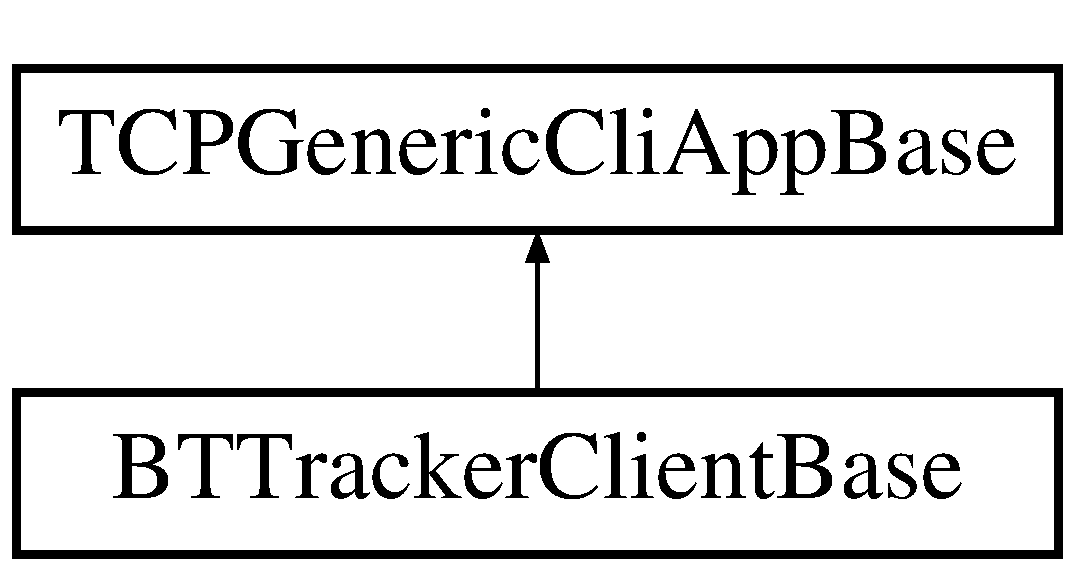
\includegraphics[height=2.000000cm]{classBTTrackerClientBase}
\end{center}
\end{figure}
\subsection*{Public Member Functions}
\begin{DoxyCompactItemize}
\item 
\hyperlink{classBTTrackerClientBase_af2daf873e282ca0f12a34ba657d801de}{B\+T\+Tracker\+Client\+Base} ()
\item 
virtual \hyperlink{classBTTrackerClientBase_a52ebc86c77b27289b4ac3d3131b6e9d3}{$\sim$\+B\+T\+Tracker\+Client\+Base} ()
\item 
size\+\_\+t \hyperlink{classBTTrackerClientBase_a65879dbc1ec398c124f27c5d4ca63552}{cstate} () const 
\item 
void \hyperlink{classBTTrackerClientBase_a4cd61fb7ac4fed418aceb9ec76489f70}{set\+Cstate} (size\+\_\+t)
\item 
const string \& \hyperlink{classBTTrackerClientBase_a25d94d6851c1a20566a73fc8bb79fae4}{tracker\+Id} () const 
\item 
void \hyperlink{classBTTrackerClientBase_a1e34cc7545623b3e60e81f82d8321f7f}{set\+Tracker\+Id} (const string \&)
\item 
size\+\_\+t \hyperlink{classBTTrackerClientBase_a3e1eee0a4b600eb25e4406af05c86822}{connect\+Give\+Up} () const 
\item 
void \hyperlink{classBTTrackerClientBase_aadbed5705c9858f1d90050dbfeca5559}{set\+Connect\+Give\+Up} (size\+\_\+t)
\item 
simtime\+\_\+t \hyperlink{classBTTrackerClientBase_a65eb496c2f438e0a9a67b5adb83c1ffc}{session\+Timeout} () const 
\item 
void \hyperlink{classBTTrackerClientBase_a85374136d41a2df83f5ffba345d8046b}{set\+Session\+Timeout} (simtime\+\_\+t)
\item 
double \hyperlink{classBTTrackerClientBase_af5b16a044b06fe75dd8bc8c399bc8b29}{reconnect\+Interval} () const 
\item 
void \hyperlink{classBTTrackerClientBase_a6c41e7aeaa0633a2742bb7ec558ac28f}{set\+Reconnect\+Interval} (double)
\item 
const string \& \hyperlink{classBTTrackerClientBase_ad56587246469f660fedef3c50c10554d}{info\+Hash} () const 
\item 
void \hyperlink{classBTTrackerClientBase_a6f764b043ac1aba4937c02818b2aa8e5}{set\+Info\+Hash} (const string \&)
\item 
const string \& \hyperlink{classBTTrackerClientBase_aaa2e7b0d4d3770dedd7baff0fbd2da45}{peer\+Id} () const 
\item 
void \hyperlink{classBTTrackerClientBase_a38b8f2500d5c39c8a1d079970985c877}{set\+Peer\+Id} (const string \&)
\item 
size\+\_\+t \hyperlink{classBTTrackerClientBase_ab0833d033c769937a3a51e39904f9fc0}{peer\+Port} () const 
\item 
void \hyperlink{classBTTrackerClientBase_aec9b615f0e50e53854df6b6eac0d83c2}{set\+Peer\+Port} (size\+\_\+t)
\item 
bool \hyperlink{classBTTrackerClientBase_a678dcdf76412fbed63bf9a8b0b9fc686}{compact} () const 
\item 
void \hyperlink{classBTTrackerClientBase_a251809d0b4ea9f07b2ca3c26fa4ea2b7}{set\+Compact} (bool)
\item 
bool \hyperlink{classBTTrackerClientBase_ae1a3c76c6a8605acb228748ca0a68ad6}{no\+Peer\+Id} () const 
\item 
void \hyperlink{classBTTrackerClientBase_a9b4700cf1790d17bc73d7a18078226cd}{set\+No\+Peer\+Id} (bool)
\item 
size\+\_\+t \hyperlink{classBTTrackerClientBase_a161caadc519753d4469377515c7a4fcf}{num\+Want} () const 
\item 
void \hyperlink{classBTTrackerClientBase_a21ee3296f8698ac6f49fec71e3caf57d}{set\+Num\+Want} (size\+\_\+t)
\item 
const string \& \hyperlink{classBTTrackerClientBase_a0137bb8858b6f40e1f82bb34a9009cff}{key} () const 
\item 
void \hyperlink{classBTTrackerClientBase_ad3c6c86644a0657a062ee7a6d312e4ad}{set\+Key} (const string \&)
\item 
virtual const char $\ast$ \hyperlink{classBTTrackerClientBase_ac2d122e57e8a049579b08214da47c0d5}{generate\+Peer\+I\+D} ()
\end{DoxyCompactItemize}
\subsection*{Protected Member Functions}
\begin{DoxyCompactItemize}
\item 
virtual void \hyperlink{classBTTrackerClientBase_ab069678d1177731f94c52620f91e6f55}{announce} ()
\item 
virtual void \hyperlink{classBTTrackerClientBase_a245a5285af4b921bc4750245b8c73e0d}{find\+And\+Set\+I\+P\+Address} ()
\item 
virtual void \hyperlink{classBTTrackerClientBase_adc7c0ed12a24c892801841a96f663a2a}{find\+And\+Set\+Announce\+Size} (c\+Message $\ast$) const 
\item 
virtual void \hyperlink{classBTTrackerClientBase_a3427a3d40ea862c9e362061e1e65c616}{initialize} ()
\item 
virtual void \hyperlink{classBTTrackerClientBase_a04f42878a2710962bbb88f96706c6dca}{handle\+Message} (c\+Message $\ast$)
\item 
virtual void \hyperlink{classBTTrackerClientBase_aa7f93bb3a652daa74b54b1eedaafc7ad}{handle\+Timer} (c\+Message $\ast$)
\item 
virtual void \hyperlink{classBTTrackerClientBase_a44eed7960a877b2b162180bc5383ef6a}{connect} ()
\item 
virtual void \hyperlink{classBTTrackerClientBase_a7ae7c9871d98d153e0c6755d18a2b9e5}{close} ()
\item 
virtual void \hyperlink{classBTTrackerClientBase_a140fb33f9b56bddc2e60c4270fc6f685}{socket\+Established} (int, void $\ast$)
\item 
virtual void \hyperlink{classBTTrackerClientBase_acccef00f80f12202e4b63b1098af1d75}{socket\+Data\+Arrived} (int, void $\ast$, c\+Packet $\ast$, bool)
\item 
virtual void \hyperlink{classBTTrackerClientBase_ad9b4cdff6c47ef5e12018fb010b608e7}{socket\+Peer\+Closed} (int, void $\ast$)
\item 
virtual void \hyperlink{classBTTrackerClientBase_a2f099a4c762287c598b449e8183f4679}{socket\+Failure} (int, void $\ast$, int)
\end{DoxyCompactItemize}
\subsection*{Protected Attributes}
\begin{DoxyCompactItemize}
\item 
c\+Message $\ast$ \hyperlink{classBTTrackerClientBase_a728682a65c38c4152152bc5a64a768cf}{evt\+Tout}
\item 
size\+\_\+t \hyperlink{classBTTrackerClientBase_a0eead109fc2d0e3cd0462b1e19f87545}{state\+\_\+var}
\item 
size\+\_\+t \hyperlink{classBTTrackerClientBase_a1d356eceda84b31bef362f262c664a71}{transient\+\_\+var}
\item 
string \hyperlink{classBTTrackerClientBase_aee1b8d7f800c7642c1bdc435e968ec3b}{tracker\+Id\+\_\+var}
\item 
I\+Pv\+X\+Address \hyperlink{classBTTrackerClientBase_a17ed36fc72a43ca1e95020de9acc5e77}{ipaddress\+\_\+var}
\item 
size\+\_\+t \hyperlink{classBTTrackerClientBase_a7cad897127fe659fd57a3bf41a3645e0}{connect\+Give\+Up\+\_\+var}
\item 
simtime\+\_\+t \hyperlink{classBTTrackerClientBase_ab3b0b46284315a9b2e71daf379b7a3ff}{session\+Timeout\+\_\+var}
\item 
simtime\+\_\+t \hyperlink{classBTTrackerClientBase_a4fb36f2c092a853cc4611b1faa51b802}{reconnect\+Interval\+\_\+var}
\item 
string \hyperlink{classBTTrackerClientBase_ade240dc1b9440fa2d6a8ba23ed8db3ae}{info\+Hash\+\_\+var}
\item 
string \hyperlink{classBTTrackerClientBase_aa9be905707abb2eb69f831ffcd9a67e8}{peer\+Id\+\_\+var}
\item 
size\+\_\+t \hyperlink{classBTTrackerClientBase_a729473eedff089d0ae0be578cc1af653}{peer\+Port\+\_\+var}
\item 
bool \hyperlink{classBTTrackerClientBase_a8a7ea410b57b218ab38ee9394951557f}{compact\+\_\+var}
\item 
bool \hyperlink{classBTTrackerClientBase_ab23d101af767f0979c9de612fb2d511e}{no\+Peer\+Id\+\_\+var}
\item 
size\+\_\+t \hyperlink{classBTTrackerClientBase_a8e15dea1f9c602da6e78d85e271092e6}{num\+Want\+\_\+var}
\item 
string \hyperlink{classBTTrackerClientBase_a7ce835ff5b9d4e65905e6ef3635ad827}{key\+\_\+var}
\end{DoxyCompactItemize}


\subsection{Detailed Description}
Bit\+Torrent protocol. Implements a tracker client as described at \href{http://wiki.theory.org/BitTorrentSpecification}{\tt http\+://wiki.\+theory.\+org/\+Bit\+Torrent\+Specification} 

\subsection{Constructor \& Destructor Documentation}
\hypertarget{classBTTrackerClientBase_af2daf873e282ca0f12a34ba657d801de}{}\index{B\+T\+Tracker\+Client\+Base@{B\+T\+Tracker\+Client\+Base}!B\+T\+Tracker\+Client\+Base@{B\+T\+Tracker\+Client\+Base}}
\index{B\+T\+Tracker\+Client\+Base@{B\+T\+Tracker\+Client\+Base}!B\+T\+Tracker\+Client\+Base@{B\+T\+Tracker\+Client\+Base}}
\subsubsection[{B\+T\+Tracker\+Client\+Base()}]{\setlength{\rightskip}{0pt plus 5cm}B\+T\+Tracker\+Client\+Base\+::\+B\+T\+Tracker\+Client\+Base (
\begin{DoxyParamCaption}
{}
\end{DoxyParamCaption}
)}\label{classBTTrackerClientBase_af2daf873e282ca0f12a34ba657d801de}
Constructor. \hypertarget{classBTTrackerClientBase_a52ebc86c77b27289b4ac3d3131b6e9d3}{}\index{B\+T\+Tracker\+Client\+Base@{B\+T\+Tracker\+Client\+Base}!````~B\+T\+Tracker\+Client\+Base@{$\sim$\+B\+T\+Tracker\+Client\+Base}}
\index{````~B\+T\+Tracker\+Client\+Base@{$\sim$\+B\+T\+Tracker\+Client\+Base}!B\+T\+Tracker\+Client\+Base@{B\+T\+Tracker\+Client\+Base}}
\subsubsection[{$\sim$\+B\+T\+Tracker\+Client\+Base()}]{\setlength{\rightskip}{0pt plus 5cm}B\+T\+Tracker\+Client\+Base\+::$\sim$\+B\+T\+Tracker\+Client\+Base (
\begin{DoxyParamCaption}
{}
\end{DoxyParamCaption}
)\hspace{0.3cm}{\ttfamily [virtual]}}\label{classBTTrackerClientBase_a52ebc86c77b27289b4ac3d3131b6e9d3}
Destructor. 

\subsection{Member Function Documentation}
\hypertarget{classBTTrackerClientBase_ab069678d1177731f94c52620f91e6f55}{}\index{B\+T\+Tracker\+Client\+Base@{B\+T\+Tracker\+Client\+Base}!announce@{announce}}
\index{announce@{announce}!B\+T\+Tracker\+Client\+Base@{B\+T\+Tracker\+Client\+Base}}
\subsubsection[{announce()}]{\setlength{\rightskip}{0pt plus 5cm}void B\+T\+Tracker\+Client\+Base\+::announce (
\begin{DoxyParamCaption}
{}
\end{DoxyParamCaption}
)\hspace{0.3cm}{\ttfamily [protected]}, {\ttfamily [virtual]}}\label{classBTTrackerClientBase_ab069678d1177731f94c52620f91e6f55}
Sends an announce to the tracker.

This method should be re-\/implemented in future subclasses in order to extend/add/change the behavior of the client. \hypertarget{classBTTrackerClientBase_a7ae7c9871d98d153e0c6755d18a2b9e5}{}\index{B\+T\+Tracker\+Client\+Base@{B\+T\+Tracker\+Client\+Base}!close@{close}}
\index{close@{close}!B\+T\+Tracker\+Client\+Base@{B\+T\+Tracker\+Client\+Base}}
\subsubsection[{close()}]{\setlength{\rightskip}{0pt plus 5cm}void B\+T\+Tracker\+Client\+Base\+::close (
\begin{DoxyParamCaption}
{}
\end{DoxyParamCaption}
)\hspace{0.3cm}{\ttfamily [protected]}, {\ttfamily [virtual]}}\label{classBTTrackerClientBase_a7ae7c9871d98d153e0c6755d18a2b9e5}
Closes an active connection \hypertarget{classBTTrackerClientBase_a678dcdf76412fbed63bf9a8b0b9fc686}{}\index{B\+T\+Tracker\+Client\+Base@{B\+T\+Tracker\+Client\+Base}!compact@{compact}}
\index{compact@{compact}!B\+T\+Tracker\+Client\+Base@{B\+T\+Tracker\+Client\+Base}}
\subsubsection[{compact() const }]{\setlength{\rightskip}{0pt plus 5cm}bool B\+T\+Tracker\+Client\+Base\+::compact (
\begin{DoxyParamCaption}
{}
\end{DoxyParamCaption}
) const}\label{classBTTrackerClientBase_a678dcdf76412fbed63bf9a8b0b9fc686}
Get the compact flag. \hypertarget{classBTTrackerClientBase_a44eed7960a877b2b162180bc5383ef6a}{}\index{B\+T\+Tracker\+Client\+Base@{B\+T\+Tracker\+Client\+Base}!connect@{connect}}
\index{connect@{connect}!B\+T\+Tracker\+Client\+Base@{B\+T\+Tracker\+Client\+Base}}
\subsubsection[{connect()}]{\setlength{\rightskip}{0pt plus 5cm}void B\+T\+Tracker\+Client\+Base\+::connect (
\begin{DoxyParamCaption}
{}
\end{DoxyParamCaption}
)\hspace{0.3cm}{\ttfamily [protected]}, {\ttfamily [virtual]}}\label{classBTTrackerClientBase_a44eed7960a877b2b162180bc5383ef6a}
Starts a new connection.

This method should be re-\/implemented in future subclasses in order to extend/add/change the behavior of the client. \hypertarget{classBTTrackerClientBase_a3e1eee0a4b600eb25e4406af05c86822}{}\index{B\+T\+Tracker\+Client\+Base@{B\+T\+Tracker\+Client\+Base}!connect\+Give\+Up@{connect\+Give\+Up}}
\index{connect\+Give\+Up@{connect\+Give\+Up}!B\+T\+Tracker\+Client\+Base@{B\+T\+Tracker\+Client\+Base}}
\subsubsection[{connect\+Give\+Up() const }]{\setlength{\rightskip}{0pt plus 5cm}size\+\_\+t B\+T\+Tracker\+Client\+Base\+::connect\+Give\+Up (
\begin{DoxyParamCaption}
{}
\end{DoxyParamCaption}
) const}\label{classBTTrackerClientBase_a3e1eee0a4b600eb25e4406af05c86822}
Get the re-\/connect tries. \hypertarget{classBTTrackerClientBase_a65879dbc1ec398c124f27c5d4ca63552}{}\index{B\+T\+Tracker\+Client\+Base@{B\+T\+Tracker\+Client\+Base}!cstate@{cstate}}
\index{cstate@{cstate}!B\+T\+Tracker\+Client\+Base@{B\+T\+Tracker\+Client\+Base}}
\subsubsection[{cstate() const }]{\setlength{\rightskip}{0pt plus 5cm}size\+\_\+t B\+T\+Tracker\+Client\+Base\+::cstate (
\begin{DoxyParamCaption}
{}
\end{DoxyParamCaption}
) const}\label{classBTTrackerClientBase_a65879dbc1ec398c124f27c5d4ca63552}
Get the state of the client. \hypertarget{classBTTrackerClientBase_adc7c0ed12a24c892801841a96f663a2a}{}\index{B\+T\+Tracker\+Client\+Base@{B\+T\+Tracker\+Client\+Base}!find\+And\+Set\+Announce\+Size@{find\+And\+Set\+Announce\+Size}}
\index{find\+And\+Set\+Announce\+Size@{find\+And\+Set\+Announce\+Size}!B\+T\+Tracker\+Client\+Base@{B\+T\+Tracker\+Client\+Base}}
\subsubsection[{find\+And\+Set\+Announce\+Size(c\+Message $\ast$) const }]{\setlength{\rightskip}{0pt plus 5cm}void B\+T\+Tracker\+Client\+Base\+::find\+And\+Set\+Announce\+Size (
\begin{DoxyParamCaption}
\item[{c\+Message $\ast$}]{msg}
\end{DoxyParamCaption}
) const\hspace{0.3cm}{\ttfamily [protected]}, {\ttfamily [virtual]}}\label{classBTTrackerClientBase_adc7c0ed12a24c892801841a96f663a2a}
Set the size of the announce message.

This method should be re-\/implemented in future subclasses in order to extend/add/change the behavior of the client. \hypertarget{classBTTrackerClientBase_a245a5285af4b921bc4750245b8c73e0d}{}\index{B\+T\+Tracker\+Client\+Base@{B\+T\+Tracker\+Client\+Base}!find\+And\+Set\+I\+P\+Address@{find\+And\+Set\+I\+P\+Address}}
\index{find\+And\+Set\+I\+P\+Address@{find\+And\+Set\+I\+P\+Address}!B\+T\+Tracker\+Client\+Base@{B\+T\+Tracker\+Client\+Base}}
\subsubsection[{find\+And\+Set\+I\+P\+Address()}]{\setlength{\rightskip}{0pt plus 5cm}void B\+T\+Tracker\+Client\+Base\+::find\+And\+Set\+I\+P\+Address (
\begin{DoxyParamCaption}
{}
\end{DoxyParamCaption}
)\hspace{0.3cm}{\ttfamily [protected]}, {\ttfamily [virtual]}}\label{classBTTrackerClientBase_a245a5285af4b921bc4750245b8c73e0d}
Find the I\+P address of the client.

This method should be re-\/implemented in future subclasses in order to extend/add/change the behavior of the client. \hypertarget{classBTTrackerClientBase_ac2d122e57e8a049579b08214da47c0d5}{}\index{B\+T\+Tracker\+Client\+Base@{B\+T\+Tracker\+Client\+Base}!generate\+Peer\+I\+D@{generate\+Peer\+I\+D}}
\index{generate\+Peer\+I\+D@{generate\+Peer\+I\+D}!B\+T\+Tracker\+Client\+Base@{B\+T\+Tracker\+Client\+Base}}
\subsubsection[{generate\+Peer\+I\+D()}]{\setlength{\rightskip}{0pt plus 5cm}const char $\ast$ B\+T\+Tracker\+Client\+Base\+::generate\+Peer\+I\+D (
\begin{DoxyParamCaption}
{}
\end{DoxyParamCaption}
)\hspace{0.3cm}{\ttfamily [virtual]}}\label{classBTTrackerClientBase_ac2d122e57e8a049579b08214da47c0d5}
Generates an Azureus-\/style 20 character long, unique peer I\+D, with\+:
\begin{DoxyItemize}
\item client I\+D = \textquotesingle{}O\+M\textquotesingle{} (O\+Mnet++)
\item version number = 0001 (See \href{http://wiki.theory.org/BitTorrentSpecification}{\tt http\+://wiki.\+theory.\+org/\+Bit\+Torrent\+Specification} for more information)
\end{DoxyItemize}

The peer I\+D is augmented with the hosting module\textquotesingle{}s name, for clarity/debugging purposes.

This method should be re-\/implemented in future subclasses in order to change the.\+way peer I\+Ds are generated. \hypertarget{classBTTrackerClientBase_a04f42878a2710962bbb88f96706c6dca}{}\index{B\+T\+Tracker\+Client\+Base@{B\+T\+Tracker\+Client\+Base}!handle\+Message@{handle\+Message}}
\index{handle\+Message@{handle\+Message}!B\+T\+Tracker\+Client\+Base@{B\+T\+Tracker\+Client\+Base}}
\subsubsection[{handle\+Message(c\+Message $\ast$)}]{\setlength{\rightskip}{0pt plus 5cm}void B\+T\+Tracker\+Client\+Base\+::handle\+Message (
\begin{DoxyParamCaption}
\item[{c\+Message $\ast$}]{msg}
\end{DoxyParamCaption}
)\hspace{0.3cm}{\ttfamily [protected]}, {\ttfamily [virtual]}}\label{classBTTrackerClientBase_a04f42878a2710962bbb88f96706c6dca}
Called each time a new message is received. \hypertarget{classBTTrackerClientBase_aa7f93bb3a652daa74b54b1eedaafc7ad}{}\index{B\+T\+Tracker\+Client\+Base@{B\+T\+Tracker\+Client\+Base}!handle\+Timer@{handle\+Timer}}
\index{handle\+Timer@{handle\+Timer}!B\+T\+Tracker\+Client\+Base@{B\+T\+Tracker\+Client\+Base}}
\subsubsection[{handle\+Timer(c\+Message $\ast$)}]{\setlength{\rightskip}{0pt plus 5cm}void B\+T\+Tracker\+Client\+Base\+::handle\+Timer (
\begin{DoxyParamCaption}
\item[{c\+Message $\ast$}]{msg}
\end{DoxyParamCaption}
)\hspace{0.3cm}{\ttfamily [protected]}, {\ttfamily [virtual]}}\label{classBTTrackerClientBase_aa7f93bb3a652daa74b54b1eedaafc7ad}
Called from \hyperlink{classBTTrackerClientBase_aa7f93bb3a652daa74b54b1eedaafc7ad}{handle\+Timer()} each time a self message or a message from btorrent\+In gate is received. \hypertarget{classBTTrackerClientBase_ad56587246469f660fedef3c50c10554d}{}\index{B\+T\+Tracker\+Client\+Base@{B\+T\+Tracker\+Client\+Base}!info\+Hash@{info\+Hash}}
\index{info\+Hash@{info\+Hash}!B\+T\+Tracker\+Client\+Base@{B\+T\+Tracker\+Client\+Base}}
\subsubsection[{info\+Hash() const }]{\setlength{\rightskip}{0pt plus 5cm}const string \& B\+T\+Tracker\+Client\+Base\+::info\+Hash (
\begin{DoxyParamCaption}
{}
\end{DoxyParamCaption}
) const}\label{classBTTrackerClientBase_ad56587246469f660fedef3c50c10554d}
Get the info hash. \hypertarget{classBTTrackerClientBase_a3427a3d40ea862c9e362061e1e65c616}{}\index{B\+T\+Tracker\+Client\+Base@{B\+T\+Tracker\+Client\+Base}!initialize@{initialize}}
\index{initialize@{initialize}!B\+T\+Tracker\+Client\+Base@{B\+T\+Tracker\+Client\+Base}}
\subsubsection[{initialize()}]{\setlength{\rightskip}{0pt plus 5cm}void B\+T\+Tracker\+Client\+Base\+::initialize (
\begin{DoxyParamCaption}
{}
\end{DoxyParamCaption}
)\hspace{0.3cm}{\ttfamily [protected]}, {\ttfamily [virtual]}}\label{classBTTrackerClientBase_a3427a3d40ea862c9e362061e1e65c616}
Called after the module creation. \hypertarget{classBTTrackerClientBase_a0137bb8858b6f40e1f82bb34a9009cff}{}\index{B\+T\+Tracker\+Client\+Base@{B\+T\+Tracker\+Client\+Base}!key@{key}}
\index{key@{key}!B\+T\+Tracker\+Client\+Base@{B\+T\+Tracker\+Client\+Base}}
\subsubsection[{key() const }]{\setlength{\rightskip}{0pt plus 5cm}const string \& B\+T\+Tracker\+Client\+Base\+::key (
\begin{DoxyParamCaption}
{}
\end{DoxyParamCaption}
) const}\label{classBTTrackerClientBase_a0137bb8858b6f40e1f82bb34a9009cff}
Get the peer\textquotesingle{}s key. \hypertarget{classBTTrackerClientBase_ae1a3c76c6a8605acb228748ca0a68ad6}{}\index{B\+T\+Tracker\+Client\+Base@{B\+T\+Tracker\+Client\+Base}!no\+Peer\+Id@{no\+Peer\+Id}}
\index{no\+Peer\+Id@{no\+Peer\+Id}!B\+T\+Tracker\+Client\+Base@{B\+T\+Tracker\+Client\+Base}}
\subsubsection[{no\+Peer\+Id() const }]{\setlength{\rightskip}{0pt plus 5cm}bool B\+T\+Tracker\+Client\+Base\+::no\+Peer\+Id (
\begin{DoxyParamCaption}
{}
\end{DoxyParamCaption}
) const}\label{classBTTrackerClientBase_ae1a3c76c6a8605acb228748ca0a68ad6}
Get the no\+\_\+peer\+\_\+id flag. \hypertarget{classBTTrackerClientBase_a161caadc519753d4469377515c7a4fcf}{}\index{B\+T\+Tracker\+Client\+Base@{B\+T\+Tracker\+Client\+Base}!num\+Want@{num\+Want}}
\index{num\+Want@{num\+Want}!B\+T\+Tracker\+Client\+Base@{B\+T\+Tracker\+Client\+Base}}
\subsubsection[{num\+Want() const }]{\setlength{\rightskip}{0pt plus 5cm}size\+\_\+t B\+T\+Tracker\+Client\+Base\+::num\+Want (
\begin{DoxyParamCaption}
{}
\end{DoxyParamCaption}
) const}\label{classBTTrackerClientBase_a161caadc519753d4469377515c7a4fcf}
Get the num\+Want peers count. \hypertarget{classBTTrackerClientBase_aaa2e7b0d4d3770dedd7baff0fbd2da45}{}\index{B\+T\+Tracker\+Client\+Base@{B\+T\+Tracker\+Client\+Base}!peer\+Id@{peer\+Id}}
\index{peer\+Id@{peer\+Id}!B\+T\+Tracker\+Client\+Base@{B\+T\+Tracker\+Client\+Base}}
\subsubsection[{peer\+Id() const }]{\setlength{\rightskip}{0pt plus 5cm}const string \& B\+T\+Tracker\+Client\+Base\+::peer\+Id (
\begin{DoxyParamCaption}
{}
\end{DoxyParamCaption}
) const}\label{classBTTrackerClientBase_aaa2e7b0d4d3770dedd7baff0fbd2da45}
Get the peer id. \hypertarget{classBTTrackerClientBase_ab0833d033c769937a3a51e39904f9fc0}{}\index{B\+T\+Tracker\+Client\+Base@{B\+T\+Tracker\+Client\+Base}!peer\+Port@{peer\+Port}}
\index{peer\+Port@{peer\+Port}!B\+T\+Tracker\+Client\+Base@{B\+T\+Tracker\+Client\+Base}}
\subsubsection[{peer\+Port() const }]{\setlength{\rightskip}{0pt plus 5cm}size\+\_\+t B\+T\+Tracker\+Client\+Base\+::peer\+Port (
\begin{DoxyParamCaption}
{}
\end{DoxyParamCaption}
) const}\label{classBTTrackerClientBase_ab0833d033c769937a3a51e39904f9fc0}
Get the peer port. \hypertarget{classBTTrackerClientBase_af5b16a044b06fe75dd8bc8c399bc8b29}{}\index{B\+T\+Tracker\+Client\+Base@{B\+T\+Tracker\+Client\+Base}!reconnect\+Interval@{reconnect\+Interval}}
\index{reconnect\+Interval@{reconnect\+Interval}!B\+T\+Tracker\+Client\+Base@{B\+T\+Tracker\+Client\+Base}}
\subsubsection[{reconnect\+Interval() const }]{\setlength{\rightskip}{0pt plus 5cm}double B\+T\+Tracker\+Client\+Base\+::reconnect\+Interval (
\begin{DoxyParamCaption}
{}
\end{DoxyParamCaption}
) const}\label{classBTTrackerClientBase_af5b16a044b06fe75dd8bc8c399bc8b29}
Get the re-\/connect interval. \hypertarget{classBTTrackerClientBase_a65eb496c2f438e0a9a67b5adb83c1ffc}{}\index{B\+T\+Tracker\+Client\+Base@{B\+T\+Tracker\+Client\+Base}!session\+Timeout@{session\+Timeout}}
\index{session\+Timeout@{session\+Timeout}!B\+T\+Tracker\+Client\+Base@{B\+T\+Tracker\+Client\+Base}}
\subsubsection[{session\+Timeout() const }]{\setlength{\rightskip}{0pt plus 5cm}simtime\+\_\+t B\+T\+Tracker\+Client\+Base\+::session\+Timeout (
\begin{DoxyParamCaption}
{}
\end{DoxyParamCaption}
) const}\label{classBTTrackerClientBase_a65eb496c2f438e0a9a67b5adb83c1ffc}
Get the session timeout (seconds). \hypertarget{classBTTrackerClientBase_a251809d0b4ea9f07b2ca3c26fa4ea2b7}{}\index{B\+T\+Tracker\+Client\+Base@{B\+T\+Tracker\+Client\+Base}!set\+Compact@{set\+Compact}}
\index{set\+Compact@{set\+Compact}!B\+T\+Tracker\+Client\+Base@{B\+T\+Tracker\+Client\+Base}}
\subsubsection[{set\+Compact(bool)}]{\setlength{\rightskip}{0pt plus 5cm}void B\+T\+Tracker\+Client\+Base\+::set\+Compact (
\begin{DoxyParamCaption}
\item[{bool}]{compact}
\end{DoxyParamCaption}
)}\label{classBTTrackerClientBase_a251809d0b4ea9f07b2ca3c26fa4ea2b7}
Set the compact flag. \hypertarget{classBTTrackerClientBase_aadbed5705c9858f1d90050dbfeca5559}{}\index{B\+T\+Tracker\+Client\+Base@{B\+T\+Tracker\+Client\+Base}!set\+Connect\+Give\+Up@{set\+Connect\+Give\+Up}}
\index{set\+Connect\+Give\+Up@{set\+Connect\+Give\+Up}!B\+T\+Tracker\+Client\+Base@{B\+T\+Tracker\+Client\+Base}}
\subsubsection[{set\+Connect\+Give\+Up(size\+\_\+t)}]{\setlength{\rightskip}{0pt plus 5cm}void B\+T\+Tracker\+Client\+Base\+::set\+Connect\+Give\+Up (
\begin{DoxyParamCaption}
\item[{size\+\_\+t}]{connect\+Give\+Up}
\end{DoxyParamCaption}
)}\label{classBTTrackerClientBase_aadbed5705c9858f1d90050dbfeca5559}
Set the re-\/connect tries. \hypertarget{classBTTrackerClientBase_a4cd61fb7ac4fed418aceb9ec76489f70}{}\index{B\+T\+Tracker\+Client\+Base@{B\+T\+Tracker\+Client\+Base}!set\+Cstate@{set\+Cstate}}
\index{set\+Cstate@{set\+Cstate}!B\+T\+Tracker\+Client\+Base@{B\+T\+Tracker\+Client\+Base}}
\subsubsection[{set\+Cstate(size\+\_\+t)}]{\setlength{\rightskip}{0pt plus 5cm}void B\+T\+Tracker\+Client\+Base\+::set\+Cstate (
\begin{DoxyParamCaption}
\item[{size\+\_\+t}]{state}
\end{DoxyParamCaption}
)}\label{classBTTrackerClientBase_a4cd61fb7ac4fed418aceb9ec76489f70}
Set the state of the client. \hypertarget{classBTTrackerClientBase_a6f764b043ac1aba4937c02818b2aa8e5}{}\index{B\+T\+Tracker\+Client\+Base@{B\+T\+Tracker\+Client\+Base}!set\+Info\+Hash@{set\+Info\+Hash}}
\index{set\+Info\+Hash@{set\+Info\+Hash}!B\+T\+Tracker\+Client\+Base@{B\+T\+Tracker\+Client\+Base}}
\subsubsection[{set\+Info\+Hash(const string \&)}]{\setlength{\rightskip}{0pt plus 5cm}void B\+T\+Tracker\+Client\+Base\+::set\+Info\+Hash (
\begin{DoxyParamCaption}
\item[{const string \&}]{info\+Hash}
\end{DoxyParamCaption}
)}\label{classBTTrackerClientBase_a6f764b043ac1aba4937c02818b2aa8e5}
Set the info hash. \hypertarget{classBTTrackerClientBase_ad3c6c86644a0657a062ee7a6d312e4ad}{}\index{B\+T\+Tracker\+Client\+Base@{B\+T\+Tracker\+Client\+Base}!set\+Key@{set\+Key}}
\index{set\+Key@{set\+Key}!B\+T\+Tracker\+Client\+Base@{B\+T\+Tracker\+Client\+Base}}
\subsubsection[{set\+Key(const string \&)}]{\setlength{\rightskip}{0pt plus 5cm}void B\+T\+Tracker\+Client\+Base\+::set\+Key (
\begin{DoxyParamCaption}
\item[{const string \&}]{key}
\end{DoxyParamCaption}
)}\label{classBTTrackerClientBase_ad3c6c86644a0657a062ee7a6d312e4ad}
Set the peer\textquotesingle{}s key. \hypertarget{classBTTrackerClientBase_a9b4700cf1790d17bc73d7a18078226cd}{}\index{B\+T\+Tracker\+Client\+Base@{B\+T\+Tracker\+Client\+Base}!set\+No\+Peer\+Id@{set\+No\+Peer\+Id}}
\index{set\+No\+Peer\+Id@{set\+No\+Peer\+Id}!B\+T\+Tracker\+Client\+Base@{B\+T\+Tracker\+Client\+Base}}
\subsubsection[{set\+No\+Peer\+Id(bool)}]{\setlength{\rightskip}{0pt plus 5cm}void B\+T\+Tracker\+Client\+Base\+::set\+No\+Peer\+Id (
\begin{DoxyParamCaption}
\item[{bool}]{no\+Peer\+Id}
\end{DoxyParamCaption}
)}\label{classBTTrackerClientBase_a9b4700cf1790d17bc73d7a18078226cd}
Set the no\+\_\+peer\+\_\+id flag. \hypertarget{classBTTrackerClientBase_a21ee3296f8698ac6f49fec71e3caf57d}{}\index{B\+T\+Tracker\+Client\+Base@{B\+T\+Tracker\+Client\+Base}!set\+Num\+Want@{set\+Num\+Want}}
\index{set\+Num\+Want@{set\+Num\+Want}!B\+T\+Tracker\+Client\+Base@{B\+T\+Tracker\+Client\+Base}}
\subsubsection[{set\+Num\+Want(size\+\_\+t)}]{\setlength{\rightskip}{0pt plus 5cm}void B\+T\+Tracker\+Client\+Base\+::set\+Num\+Want (
\begin{DoxyParamCaption}
\item[{size\+\_\+t}]{num\+Want}
\end{DoxyParamCaption}
)}\label{classBTTrackerClientBase_a21ee3296f8698ac6f49fec71e3caf57d}
Set the num\+Want peers count. \hypertarget{classBTTrackerClientBase_a38b8f2500d5c39c8a1d079970985c877}{}\index{B\+T\+Tracker\+Client\+Base@{B\+T\+Tracker\+Client\+Base}!set\+Peer\+Id@{set\+Peer\+Id}}
\index{set\+Peer\+Id@{set\+Peer\+Id}!B\+T\+Tracker\+Client\+Base@{B\+T\+Tracker\+Client\+Base}}
\subsubsection[{set\+Peer\+Id(const string \&)}]{\setlength{\rightskip}{0pt plus 5cm}void B\+T\+Tracker\+Client\+Base\+::set\+Peer\+Id (
\begin{DoxyParamCaption}
\item[{const string \&}]{peer\+Id}
\end{DoxyParamCaption}
)}\label{classBTTrackerClientBase_a38b8f2500d5c39c8a1d079970985c877}
Set the peer id. \hypertarget{classBTTrackerClientBase_aec9b615f0e50e53854df6b6eac0d83c2}{}\index{B\+T\+Tracker\+Client\+Base@{B\+T\+Tracker\+Client\+Base}!set\+Peer\+Port@{set\+Peer\+Port}}
\index{set\+Peer\+Port@{set\+Peer\+Port}!B\+T\+Tracker\+Client\+Base@{B\+T\+Tracker\+Client\+Base}}
\subsubsection[{set\+Peer\+Port(size\+\_\+t)}]{\setlength{\rightskip}{0pt plus 5cm}void B\+T\+Tracker\+Client\+Base\+::set\+Peer\+Port (
\begin{DoxyParamCaption}
\item[{size\+\_\+t}]{peer\+Port}
\end{DoxyParamCaption}
)}\label{classBTTrackerClientBase_aec9b615f0e50e53854df6b6eac0d83c2}
Set the peer port. \hypertarget{classBTTrackerClientBase_a6c41e7aeaa0633a2742bb7ec558ac28f}{}\index{B\+T\+Tracker\+Client\+Base@{B\+T\+Tracker\+Client\+Base}!set\+Reconnect\+Interval@{set\+Reconnect\+Interval}}
\index{set\+Reconnect\+Interval@{set\+Reconnect\+Interval}!B\+T\+Tracker\+Client\+Base@{B\+T\+Tracker\+Client\+Base}}
\subsubsection[{set\+Reconnect\+Interval(double)}]{\setlength{\rightskip}{0pt plus 5cm}void B\+T\+Tracker\+Client\+Base\+::set\+Reconnect\+Interval (
\begin{DoxyParamCaption}
\item[{double}]{reconnect\+Interval}
\end{DoxyParamCaption}
)}\label{classBTTrackerClientBase_a6c41e7aeaa0633a2742bb7ec558ac28f}
Set the re-\/connect interval. \hypertarget{classBTTrackerClientBase_a85374136d41a2df83f5ffba345d8046b}{}\index{B\+T\+Tracker\+Client\+Base@{B\+T\+Tracker\+Client\+Base}!set\+Session\+Timeout@{set\+Session\+Timeout}}
\index{set\+Session\+Timeout@{set\+Session\+Timeout}!B\+T\+Tracker\+Client\+Base@{B\+T\+Tracker\+Client\+Base}}
\subsubsection[{set\+Session\+Timeout(simtime\+\_\+t)}]{\setlength{\rightskip}{0pt plus 5cm}void B\+T\+Tracker\+Client\+Base\+::set\+Session\+Timeout (
\begin{DoxyParamCaption}
\item[{simtime\+\_\+t}]{session\+Timeout}
\end{DoxyParamCaption}
)}\label{classBTTrackerClientBase_a85374136d41a2df83f5ffba345d8046b}
Set the session timeout (seconds). \hypertarget{classBTTrackerClientBase_a1e34cc7545623b3e60e81f82d8321f7f}{}\index{B\+T\+Tracker\+Client\+Base@{B\+T\+Tracker\+Client\+Base}!set\+Tracker\+Id@{set\+Tracker\+Id}}
\index{set\+Tracker\+Id@{set\+Tracker\+Id}!B\+T\+Tracker\+Client\+Base@{B\+T\+Tracker\+Client\+Base}}
\subsubsection[{set\+Tracker\+Id(const string \&)}]{\setlength{\rightskip}{0pt plus 5cm}void B\+T\+Tracker\+Client\+Base\+::set\+Tracker\+Id (
\begin{DoxyParamCaption}
\item[{const string \&}]{tracker\+Id}
\end{DoxyParamCaption}
)}\label{classBTTrackerClientBase_a1e34cc7545623b3e60e81f82d8321f7f}
Set the tracker id. \hypertarget{classBTTrackerClientBase_acccef00f80f12202e4b63b1098af1d75}{}\index{B\+T\+Tracker\+Client\+Base@{B\+T\+Tracker\+Client\+Base}!socket\+Data\+Arrived@{socket\+Data\+Arrived}}
\index{socket\+Data\+Arrived@{socket\+Data\+Arrived}!B\+T\+Tracker\+Client\+Base@{B\+T\+Tracker\+Client\+Base}}
\subsubsection[{socket\+Data\+Arrived(int, void $\ast$, c\+Packet $\ast$, bool)}]{\setlength{\rightskip}{0pt plus 5cm}void B\+T\+Tracker\+Client\+Base\+::socket\+Data\+Arrived (
\begin{DoxyParamCaption}
\item[{int}]{conn\+Id, }
\item[{void $\ast$}]{ptr, }
\item[{c\+Packet $\ast$}]{msg, }
\item[{bool}]{urgent}
\end{DoxyParamCaption}
)\hspace{0.3cm}{\ttfamily [protected]}, {\ttfamily [virtual]}}\label{classBTTrackerClientBase_acccef00f80f12202e4b63b1098af1d75}
Handles the response from the tracker.

This method should be re-\/implemented in future subclasses in order to extend/add/change the behavior of the client. \hypertarget{classBTTrackerClientBase_a140fb33f9b56bddc2e60c4270fc6f685}{}\index{B\+T\+Tracker\+Client\+Base@{B\+T\+Tracker\+Client\+Base}!socket\+Established@{socket\+Established}}
\index{socket\+Established@{socket\+Established}!B\+T\+Tracker\+Client\+Base@{B\+T\+Tracker\+Client\+Base}}
\subsubsection[{socket\+Established(int, void $\ast$)}]{\setlength{\rightskip}{0pt plus 5cm}void B\+T\+Tracker\+Client\+Base\+::socket\+Established (
\begin{DoxyParamCaption}
\item[{int}]{conn\+Id, }
\item[{void $\ast$}]{ptr}
\end{DoxyParamCaption}
)\hspace{0.3cm}{\ttfamily [protected]}, {\ttfamily [virtual]}}\label{classBTTrackerClientBase_a140fb33f9b56bddc2e60c4270fc6f685}
Starts a session and performs some logging.

This method should be re-\/implemented in future subclasses in order to extend/add/change the behavior of the client. \hypertarget{classBTTrackerClientBase_a2f099a4c762287c598b449e8183f4679}{}\index{B\+T\+Tracker\+Client\+Base@{B\+T\+Tracker\+Client\+Base}!socket\+Failure@{socket\+Failure}}
\index{socket\+Failure@{socket\+Failure}!B\+T\+Tracker\+Client\+Base@{B\+T\+Tracker\+Client\+Base}}
\subsubsection[{socket\+Failure(int, void $\ast$, int)}]{\setlength{\rightskip}{0pt plus 5cm}void B\+T\+Tracker\+Client\+Base\+::socket\+Failure (
\begin{DoxyParamCaption}
\item[{int}]{conn\+Id, }
\item[{void $\ast$}]{your\+Ptr, }
\item[{int}]{code}
\end{DoxyParamCaption}
)\hspace{0.3cm}{\ttfamily [protected]}, {\ttfamily [virtual]}}\label{classBTTrackerClientBase_a2f099a4c762287c598b449e8183f4679}
Handles connection failures.

This method should be re-\/implemented in future subclasses in order to extend/add/change the behavior of the client. \hypertarget{classBTTrackerClientBase_ad9b4cdff6c47ef5e12018fb010b608e7}{}\index{B\+T\+Tracker\+Client\+Base@{B\+T\+Tracker\+Client\+Base}!socket\+Peer\+Closed@{socket\+Peer\+Closed}}
\index{socket\+Peer\+Closed@{socket\+Peer\+Closed}!B\+T\+Tracker\+Client\+Base@{B\+T\+Tracker\+Client\+Base}}
\subsubsection[{socket\+Peer\+Closed(int, void $\ast$)}]{\setlength{\rightskip}{0pt plus 5cm}void B\+T\+Tracker\+Client\+Base\+::socket\+Peer\+Closed (
\begin{DoxyParamCaption}
\item[{int}]{conn\+Id, }
\item[{void $\ast$}]{your\+Ptr}
\end{DoxyParamCaption}
)\hspace{0.3cm}{\ttfamily [protected]}, {\ttfamily [virtual]}}\label{classBTTrackerClientBase_ad9b4cdff6c47ef5e12018fb010b608e7}
Handles the connection teardown.

This method should be re-\/implemented in future subclasses in order to extend/add/change the behavior of the client. \hypertarget{classBTTrackerClientBase_a25d94d6851c1a20566a73fc8bb79fae4}{}\index{B\+T\+Tracker\+Client\+Base@{B\+T\+Tracker\+Client\+Base}!tracker\+Id@{tracker\+Id}}
\index{tracker\+Id@{tracker\+Id}!B\+T\+Tracker\+Client\+Base@{B\+T\+Tracker\+Client\+Base}}
\subsubsection[{tracker\+Id() const }]{\setlength{\rightskip}{0pt plus 5cm}const string \& B\+T\+Tracker\+Client\+Base\+::tracker\+Id (
\begin{DoxyParamCaption}
{}
\end{DoxyParamCaption}
) const}\label{classBTTrackerClientBase_a25d94d6851c1a20566a73fc8bb79fae4}
Get the tracker id. 

\subsection{Member Data Documentation}
\hypertarget{classBTTrackerClientBase_a8a7ea410b57b218ab38ee9394951557f}{}\index{B\+T\+Tracker\+Client\+Base@{B\+T\+Tracker\+Client\+Base}!compact\+\_\+var@{compact\+\_\+var}}
\index{compact\+\_\+var@{compact\+\_\+var}!B\+T\+Tracker\+Client\+Base@{B\+T\+Tracker\+Client\+Base}}
\subsubsection[{compact\+\_\+var}]{\setlength{\rightskip}{0pt plus 5cm}bool B\+T\+Tracker\+Client\+Base\+::compact\+\_\+var\hspace{0.3cm}{\ttfamily [protected]}}\label{classBTTrackerClientBase_a8a7ea410b57b218ab38ee9394951557f}
\hypertarget{classBTTrackerClientBase_a7cad897127fe659fd57a3bf41a3645e0}{}\index{B\+T\+Tracker\+Client\+Base@{B\+T\+Tracker\+Client\+Base}!connect\+Give\+Up\+\_\+var@{connect\+Give\+Up\+\_\+var}}
\index{connect\+Give\+Up\+\_\+var@{connect\+Give\+Up\+\_\+var}!B\+T\+Tracker\+Client\+Base@{B\+T\+Tracker\+Client\+Base}}
\subsubsection[{connect\+Give\+Up\+\_\+var}]{\setlength{\rightskip}{0pt plus 5cm}size\+\_\+t B\+T\+Tracker\+Client\+Base\+::connect\+Give\+Up\+\_\+var\hspace{0.3cm}{\ttfamily [protected]}}\label{classBTTrackerClientBase_a7cad897127fe659fd57a3bf41a3645e0}
\hypertarget{classBTTrackerClientBase_a728682a65c38c4152152bc5a64a768cf}{}\index{B\+T\+Tracker\+Client\+Base@{B\+T\+Tracker\+Client\+Base}!evt\+Tout@{evt\+Tout}}
\index{evt\+Tout@{evt\+Tout}!B\+T\+Tracker\+Client\+Base@{B\+T\+Tracker\+Client\+Base}}
\subsubsection[{evt\+Tout}]{\setlength{\rightskip}{0pt plus 5cm}c\+Message$\ast$ B\+T\+Tracker\+Client\+Base\+::evt\+Tout\hspace{0.3cm}{\ttfamily [protected]}}\label{classBTTrackerClientBase_a728682a65c38c4152152bc5a64a768cf}
\hypertarget{classBTTrackerClientBase_ade240dc1b9440fa2d6a8ba23ed8db3ae}{}\index{B\+T\+Tracker\+Client\+Base@{B\+T\+Tracker\+Client\+Base}!info\+Hash\+\_\+var@{info\+Hash\+\_\+var}}
\index{info\+Hash\+\_\+var@{info\+Hash\+\_\+var}!B\+T\+Tracker\+Client\+Base@{B\+T\+Tracker\+Client\+Base}}
\subsubsection[{info\+Hash\+\_\+var}]{\setlength{\rightskip}{0pt plus 5cm}string B\+T\+Tracker\+Client\+Base\+::info\+Hash\+\_\+var\hspace{0.3cm}{\ttfamily [protected]}}\label{classBTTrackerClientBase_ade240dc1b9440fa2d6a8ba23ed8db3ae}
\hypertarget{classBTTrackerClientBase_a17ed36fc72a43ca1e95020de9acc5e77}{}\index{B\+T\+Tracker\+Client\+Base@{B\+T\+Tracker\+Client\+Base}!ipaddress\+\_\+var@{ipaddress\+\_\+var}}
\index{ipaddress\+\_\+var@{ipaddress\+\_\+var}!B\+T\+Tracker\+Client\+Base@{B\+T\+Tracker\+Client\+Base}}
\subsubsection[{ipaddress\+\_\+var}]{\setlength{\rightskip}{0pt plus 5cm}I\+Pv\+X\+Address B\+T\+Tracker\+Client\+Base\+::ipaddress\+\_\+var\hspace{0.3cm}{\ttfamily [protected]}}\label{classBTTrackerClientBase_a17ed36fc72a43ca1e95020de9acc5e77}
\hypertarget{classBTTrackerClientBase_a7ce835ff5b9d4e65905e6ef3635ad827}{}\index{B\+T\+Tracker\+Client\+Base@{B\+T\+Tracker\+Client\+Base}!key\+\_\+var@{key\+\_\+var}}
\index{key\+\_\+var@{key\+\_\+var}!B\+T\+Tracker\+Client\+Base@{B\+T\+Tracker\+Client\+Base}}
\subsubsection[{key\+\_\+var}]{\setlength{\rightskip}{0pt plus 5cm}string B\+T\+Tracker\+Client\+Base\+::key\+\_\+var\hspace{0.3cm}{\ttfamily [protected]}}\label{classBTTrackerClientBase_a7ce835ff5b9d4e65905e6ef3635ad827}
\hypertarget{classBTTrackerClientBase_ab23d101af767f0979c9de612fb2d511e}{}\index{B\+T\+Tracker\+Client\+Base@{B\+T\+Tracker\+Client\+Base}!no\+Peer\+Id\+\_\+var@{no\+Peer\+Id\+\_\+var}}
\index{no\+Peer\+Id\+\_\+var@{no\+Peer\+Id\+\_\+var}!B\+T\+Tracker\+Client\+Base@{B\+T\+Tracker\+Client\+Base}}
\subsubsection[{no\+Peer\+Id\+\_\+var}]{\setlength{\rightskip}{0pt plus 5cm}bool B\+T\+Tracker\+Client\+Base\+::no\+Peer\+Id\+\_\+var\hspace{0.3cm}{\ttfamily [protected]}}\label{classBTTrackerClientBase_ab23d101af767f0979c9de612fb2d511e}
\hypertarget{classBTTrackerClientBase_a8e15dea1f9c602da6e78d85e271092e6}{}\index{B\+T\+Tracker\+Client\+Base@{B\+T\+Tracker\+Client\+Base}!num\+Want\+\_\+var@{num\+Want\+\_\+var}}
\index{num\+Want\+\_\+var@{num\+Want\+\_\+var}!B\+T\+Tracker\+Client\+Base@{B\+T\+Tracker\+Client\+Base}}
\subsubsection[{num\+Want\+\_\+var}]{\setlength{\rightskip}{0pt plus 5cm}size\+\_\+t B\+T\+Tracker\+Client\+Base\+::num\+Want\+\_\+var\hspace{0.3cm}{\ttfamily [protected]}}\label{classBTTrackerClientBase_a8e15dea1f9c602da6e78d85e271092e6}
\hypertarget{classBTTrackerClientBase_aa9be905707abb2eb69f831ffcd9a67e8}{}\index{B\+T\+Tracker\+Client\+Base@{B\+T\+Tracker\+Client\+Base}!peer\+Id\+\_\+var@{peer\+Id\+\_\+var}}
\index{peer\+Id\+\_\+var@{peer\+Id\+\_\+var}!B\+T\+Tracker\+Client\+Base@{B\+T\+Tracker\+Client\+Base}}
\subsubsection[{peer\+Id\+\_\+var}]{\setlength{\rightskip}{0pt plus 5cm}string B\+T\+Tracker\+Client\+Base\+::peer\+Id\+\_\+var\hspace{0.3cm}{\ttfamily [protected]}}\label{classBTTrackerClientBase_aa9be905707abb2eb69f831ffcd9a67e8}
\hypertarget{classBTTrackerClientBase_a729473eedff089d0ae0be578cc1af653}{}\index{B\+T\+Tracker\+Client\+Base@{B\+T\+Tracker\+Client\+Base}!peer\+Port\+\_\+var@{peer\+Port\+\_\+var}}
\index{peer\+Port\+\_\+var@{peer\+Port\+\_\+var}!B\+T\+Tracker\+Client\+Base@{B\+T\+Tracker\+Client\+Base}}
\subsubsection[{peer\+Port\+\_\+var}]{\setlength{\rightskip}{0pt plus 5cm}size\+\_\+t B\+T\+Tracker\+Client\+Base\+::peer\+Port\+\_\+var\hspace{0.3cm}{\ttfamily [protected]}}\label{classBTTrackerClientBase_a729473eedff089d0ae0be578cc1af653}
\hypertarget{classBTTrackerClientBase_a4fb36f2c092a853cc4611b1faa51b802}{}\index{B\+T\+Tracker\+Client\+Base@{B\+T\+Tracker\+Client\+Base}!reconnect\+Interval\+\_\+var@{reconnect\+Interval\+\_\+var}}
\index{reconnect\+Interval\+\_\+var@{reconnect\+Interval\+\_\+var}!B\+T\+Tracker\+Client\+Base@{B\+T\+Tracker\+Client\+Base}}
\subsubsection[{reconnect\+Interval\+\_\+var}]{\setlength{\rightskip}{0pt plus 5cm}simtime\+\_\+t B\+T\+Tracker\+Client\+Base\+::reconnect\+Interval\+\_\+var\hspace{0.3cm}{\ttfamily [protected]}}\label{classBTTrackerClientBase_a4fb36f2c092a853cc4611b1faa51b802}
\hypertarget{classBTTrackerClientBase_ab3b0b46284315a9b2e71daf379b7a3ff}{}\index{B\+T\+Tracker\+Client\+Base@{B\+T\+Tracker\+Client\+Base}!session\+Timeout\+\_\+var@{session\+Timeout\+\_\+var}}
\index{session\+Timeout\+\_\+var@{session\+Timeout\+\_\+var}!B\+T\+Tracker\+Client\+Base@{B\+T\+Tracker\+Client\+Base}}
\subsubsection[{session\+Timeout\+\_\+var}]{\setlength{\rightskip}{0pt plus 5cm}simtime\+\_\+t B\+T\+Tracker\+Client\+Base\+::session\+Timeout\+\_\+var\hspace{0.3cm}{\ttfamily [protected]}}\label{classBTTrackerClientBase_ab3b0b46284315a9b2e71daf379b7a3ff}
\hypertarget{classBTTrackerClientBase_a0eead109fc2d0e3cd0462b1e19f87545}{}\index{B\+T\+Tracker\+Client\+Base@{B\+T\+Tracker\+Client\+Base}!state\+\_\+var@{state\+\_\+var}}
\index{state\+\_\+var@{state\+\_\+var}!B\+T\+Tracker\+Client\+Base@{B\+T\+Tracker\+Client\+Base}}
\subsubsection[{state\+\_\+var}]{\setlength{\rightskip}{0pt plus 5cm}size\+\_\+t B\+T\+Tracker\+Client\+Base\+::state\+\_\+var\hspace{0.3cm}{\ttfamily [protected]}}\label{classBTTrackerClientBase_a0eead109fc2d0e3cd0462b1e19f87545}
\hypertarget{classBTTrackerClientBase_aee1b8d7f800c7642c1bdc435e968ec3b}{}\index{B\+T\+Tracker\+Client\+Base@{B\+T\+Tracker\+Client\+Base}!tracker\+Id\+\_\+var@{tracker\+Id\+\_\+var}}
\index{tracker\+Id\+\_\+var@{tracker\+Id\+\_\+var}!B\+T\+Tracker\+Client\+Base@{B\+T\+Tracker\+Client\+Base}}
\subsubsection[{tracker\+Id\+\_\+var}]{\setlength{\rightskip}{0pt plus 5cm}string B\+T\+Tracker\+Client\+Base\+::tracker\+Id\+\_\+var\hspace{0.3cm}{\ttfamily [protected]}}\label{classBTTrackerClientBase_aee1b8d7f800c7642c1bdc435e968ec3b}
\hypertarget{classBTTrackerClientBase_a1d356eceda84b31bef362f262c664a71}{}\index{B\+T\+Tracker\+Client\+Base@{B\+T\+Tracker\+Client\+Base}!transient\+\_\+var@{transient\+\_\+var}}
\index{transient\+\_\+var@{transient\+\_\+var}!B\+T\+Tracker\+Client\+Base@{B\+T\+Tracker\+Client\+Base}}
\subsubsection[{transient\+\_\+var}]{\setlength{\rightskip}{0pt plus 5cm}size\+\_\+t B\+T\+Tracker\+Client\+Base\+::transient\+\_\+var\hspace{0.3cm}{\ttfamily [protected]}}\label{classBTTrackerClientBase_a1d356eceda84b31bef362f262c664a71}


The documentation for this class was generated from the following files\+:\begin{DoxyCompactItemize}
\item 
\hyperlink{BTTrackerClientBase_8h}{B\+T\+Tracker\+Client\+Base.\+h}\item 
\hyperlink{BTTrackerClientBase_8cc}{B\+T\+Tracker\+Client\+Base.\+cc}\end{DoxyCompactItemize}

\hypertarget{classBTTrackerClientHandlerBase}{}\section{B\+T\+Tracker\+Client\+Handler\+Base Class Reference}
\label{classBTTrackerClientHandlerBase}\index{B\+T\+Tracker\+Client\+Handler\+Base@{B\+T\+Tracker\+Client\+Handler\+Base}}


{\ttfamily \#include $<$B\+T\+Tracker\+Base.\+h$>$}

Inheritance diagram for B\+T\+Tracker\+Client\+Handler\+Base\+:\begin{figure}[H]
\begin{center}
\leavevmode
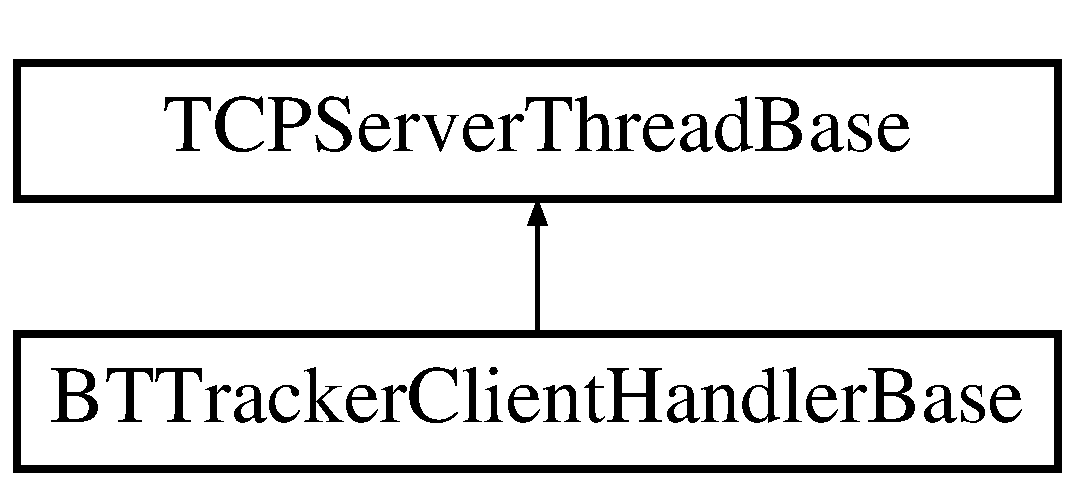
\includegraphics[height=2.000000cm]{classBTTrackerClientHandlerBase}
\end{center}
\end{figure}
\subsection*{Public Member Functions}
\begin{DoxyCompactItemize}
\item 
\hyperlink{classBTTrackerClientHandlerBase_a47bb3ebcd53cbe2c5e97761daf238848}{B\+T\+Tracker\+Client\+Handler\+Base} ()
\item 
virtual \hyperlink{classBTTrackerClientHandlerBase_a7e6bb440aeb7dc131534bddb87f8e4bf}{$\sim$\+B\+T\+Tracker\+Client\+Handler\+Base} ()
\item 
size\+\_\+t \hyperlink{classBTTrackerClientHandlerBase_a97fe99f749f9c35265a869be509ebb97}{tstate} () const 
\item 
void \hyperlink{classBTTrackerClientHandlerBase_a1ce8a476cd3678af5b6d1a6722d5dac1}{set\+Tstate} (size\+\_\+t state)
\item 
\hyperlink{classBTTrackerBase}{B\+T\+Tracker\+Base} $\ast$ \hyperlink{classBTTrackerClientHandlerBase_a8d94ff69bfee7c7fec56ff10b023190e}{host\+Module} ()
\end{DoxyCompactItemize}
\subsection*{Protected Member Functions}
\begin{DoxyCompactItemize}
\item 
virtual int \hyperlink{classBTTrackerClientHandlerBase_a08b80c81147a46c822974fc45a5abc03}{process\+Announce} (\hyperlink{classBTTrackerMsgAnnounce}{B\+T\+Tracker\+Msg\+Announce} $\ast$)
\item 
virtual void \hyperlink{classBTTrackerClientHandlerBase_a5866e5c45a061fe832b117eb7203021f}{send\+Response} (int, \hyperlink{classBTTrackerMsgAnnounce}{B\+T\+Tracker\+Msg\+Announce} $\ast$)
\item 
virtual void \hyperlink{classBTTrackerClientHandlerBase_ad736dafdf1a33bdc269cc095633aa525}{fill\+Peers\+In\+Response} (\hyperlink{classBTTrackerMsgResponse}{B\+T\+Tracker\+Msg\+Response} $\ast$, bool, bool)
\item 
virtual void \hyperlink{classBTTrackerClientHandlerBase_aab404299d6998b7e1d25bcd44797d203}{find\+And\+Set\+Response\+Size} (\hyperlink{classBTTrackerMsgResponse}{B\+T\+Tracker\+Msg\+Response} $\ast$, bool, bool)
\item 
size\+\_\+t \hyperlink{classBTTrackerClientHandlerBase_af3f5db2319771924d2768867d1e645f9}{size\+Of\+Str\+Int} (size\+\_\+t) const 
\item 
virtual void \hyperlink{classBTTrackerClientHandlerBase_a169bd0bce2bc7d184b968e49bc6af07a}{established} ()
\item 
virtual void \hyperlink{classBTTrackerClientHandlerBase_aade96a45939d0424c55c5285cacc2f51}{data\+Arrived} (c\+Message $\ast$, bool)
\item 
virtual void \hyperlink{classBTTrackerClientHandlerBase_aa5f6520bb9f47a19e5113de551639fcb}{timer\+Expired} (c\+Message $\ast$)
\item 
virtual void \hyperlink{classBTTrackerClientHandlerBase_a2fc1e4ee37fc117ac76ee1b0ed60627e}{peer\+Closed} ()
\end{DoxyCompactItemize}
\subsection*{Protected Attributes}
\begin{DoxyCompactItemize}
\item 
c\+Message $\ast$ \hyperlink{classBTTrackerClientHandlerBase_a8291f72257d451243e30b1a0b77ed1e6}{evt\+Tout}
\item 
size\+\_\+t \hyperlink{classBTTrackerClientHandlerBase_a1f5c8ad3f3fddc535e349468eb3ac526}{state\+\_\+var}
\item 
int \hyperlink{classBTTrackerClientHandlerBase_ae06f0ce4f1021ec9cc94f8900dac50b5}{c\+Peer}
\end{DoxyCompactItemize}


\subsection{Detailed Description}
Bit\+Torrent protocol. The connection handler thread. Spawned from Bit\+Torrent\+Tracker\+Base each time a new announce is made. 

\subsection{Constructor \& Destructor Documentation}
\hypertarget{classBTTrackerClientHandlerBase_a47bb3ebcd53cbe2c5e97761daf238848}{}\index{B\+T\+Tracker\+Client\+Handler\+Base@{B\+T\+Tracker\+Client\+Handler\+Base}!B\+T\+Tracker\+Client\+Handler\+Base@{B\+T\+Tracker\+Client\+Handler\+Base}}
\index{B\+T\+Tracker\+Client\+Handler\+Base@{B\+T\+Tracker\+Client\+Handler\+Base}!B\+T\+Tracker\+Client\+Handler\+Base@{B\+T\+Tracker\+Client\+Handler\+Base}}
\subsubsection[{B\+T\+Tracker\+Client\+Handler\+Base()}]{\setlength{\rightskip}{0pt plus 5cm}B\+T\+Tracker\+Client\+Handler\+Base\+::\+B\+T\+Tracker\+Client\+Handler\+Base (
\begin{DoxyParamCaption}
{}
\end{DoxyParamCaption}
)}\label{classBTTrackerClientHandlerBase_a47bb3ebcd53cbe2c5e97761daf238848}
Constructor. \hypertarget{classBTTrackerClientHandlerBase_a7e6bb440aeb7dc131534bddb87f8e4bf}{}\index{B\+T\+Tracker\+Client\+Handler\+Base@{B\+T\+Tracker\+Client\+Handler\+Base}!````~B\+T\+Tracker\+Client\+Handler\+Base@{$\sim$\+B\+T\+Tracker\+Client\+Handler\+Base}}
\index{````~B\+T\+Tracker\+Client\+Handler\+Base@{$\sim$\+B\+T\+Tracker\+Client\+Handler\+Base}!B\+T\+Tracker\+Client\+Handler\+Base@{B\+T\+Tracker\+Client\+Handler\+Base}}
\subsubsection[{$\sim$\+B\+T\+Tracker\+Client\+Handler\+Base()}]{\setlength{\rightskip}{0pt plus 5cm}B\+T\+Tracker\+Client\+Handler\+Base\+::$\sim$\+B\+T\+Tracker\+Client\+Handler\+Base (
\begin{DoxyParamCaption}
{}
\end{DoxyParamCaption}
)\hspace{0.3cm}{\ttfamily [virtual]}}\label{classBTTrackerClientHandlerBase_a7e6bb440aeb7dc131534bddb87f8e4bf}
Destructor. 

\subsection{Member Function Documentation}
\hypertarget{classBTTrackerClientHandlerBase_aade96a45939d0424c55c5285cacc2f51}{}\index{B\+T\+Tracker\+Client\+Handler\+Base@{B\+T\+Tracker\+Client\+Handler\+Base}!data\+Arrived@{data\+Arrived}}
\index{data\+Arrived@{data\+Arrived}!B\+T\+Tracker\+Client\+Handler\+Base@{B\+T\+Tracker\+Client\+Handler\+Base}}
\subsubsection[{data\+Arrived(c\+Message $\ast$, bool)}]{\setlength{\rightskip}{0pt plus 5cm}void B\+T\+Tracker\+Client\+Handler\+Base\+::data\+Arrived (
\begin{DoxyParamCaption}
\item[{c\+Message $\ast$}]{msg, }
\item[{bool}]{urgent}
\end{DoxyParamCaption}
)\hspace{0.3cm}{\ttfamily [protected]}, {\ttfamily [virtual]}}\label{classBTTrackerClientHandlerBase_aade96a45939d0424c55c5285cacc2f51}
Handles the reception of an announce.

This method should re-\/implemented in future subclasses in order to extend/add/change the behavior of the tracker. \hypertarget{classBTTrackerClientHandlerBase_a169bd0bce2bc7d184b968e49bc6af07a}{}\index{B\+T\+Tracker\+Client\+Handler\+Base@{B\+T\+Tracker\+Client\+Handler\+Base}!established@{established}}
\index{established@{established}!B\+T\+Tracker\+Client\+Handler\+Base@{B\+T\+Tracker\+Client\+Handler\+Base}}
\subsubsection[{established()}]{\setlength{\rightskip}{0pt plus 5cm}void B\+T\+Tracker\+Client\+Handler\+Base\+::established (
\begin{DoxyParamCaption}
{}
\end{DoxyParamCaption}
)\hspace{0.3cm}{\ttfamily [protected]}, {\ttfamily [virtual]}}\label{classBTTrackerClientHandlerBase_a169bd0bce2bc7d184b968e49bc6af07a}
Initializes the session variables and performs some logging.

This method should re-\/implemented in future subclasses in order to extend/add/change the behavior of the tracker. \hypertarget{classBTTrackerClientHandlerBase_ad736dafdf1a33bdc269cc095633aa525}{}\index{B\+T\+Tracker\+Client\+Handler\+Base@{B\+T\+Tracker\+Client\+Handler\+Base}!fill\+Peers\+In\+Response@{fill\+Peers\+In\+Response}}
\index{fill\+Peers\+In\+Response@{fill\+Peers\+In\+Response}!B\+T\+Tracker\+Client\+Handler\+Base@{B\+T\+Tracker\+Client\+Handler\+Base}}
\subsubsection[{fill\+Peers\+In\+Response(\+B\+T\+Tracker\+Msg\+Response $\ast$, bool, bool)}]{\setlength{\rightskip}{0pt plus 5cm}void B\+T\+Tracker\+Client\+Handler\+Base\+::fill\+Peers\+In\+Response (
\begin{DoxyParamCaption}
\item[{{\bf B\+T\+Tracker\+Msg\+Response} $\ast$}]{rmsg, }
\item[{bool}]{seed, }
\item[{bool}]{no\+\_\+peer\+\_\+id}
\end{DoxyParamCaption}
)\hspace{0.3cm}{\ttfamily [protected]}, {\ttfamily [virtual]}}\label{classBTTrackerClientHandlerBase_ad736dafdf1a33bdc269cc095633aa525}
Fill the response with peers.

This method should re-\/implemented in future subclasses in order to extend/add/change the behavior of the tracker. \hypertarget{classBTTrackerClientHandlerBase_aab404299d6998b7e1d25bcd44797d203}{}\index{B\+T\+Tracker\+Client\+Handler\+Base@{B\+T\+Tracker\+Client\+Handler\+Base}!find\+And\+Set\+Response\+Size@{find\+And\+Set\+Response\+Size}}
\index{find\+And\+Set\+Response\+Size@{find\+And\+Set\+Response\+Size}!B\+T\+Tracker\+Client\+Handler\+Base@{B\+T\+Tracker\+Client\+Handler\+Base}}
\subsubsection[{find\+And\+Set\+Response\+Size(\+B\+T\+Tracker\+Msg\+Response $\ast$, bool, bool)}]{\setlength{\rightskip}{0pt plus 5cm}void B\+T\+Tracker\+Client\+Handler\+Base\+::find\+And\+Set\+Response\+Size (
\begin{DoxyParamCaption}
\item[{{\bf B\+T\+Tracker\+Msg\+Response} $\ast$}]{rmsg, }
\item[{bool}]{compact, }
\item[{bool}]{no\+\_\+peer\+\_\+id}
\end{DoxyParamCaption}
)\hspace{0.3cm}{\ttfamily [protected]}, {\ttfamily [virtual]}}\label{classBTTrackerClientHandlerBase_aab404299d6998b7e1d25bcd44797d203}
Set the size of the response message.

This method should re-\/implemented in future subclasses in order to extend/add/change the behavior of the tracker. \hypertarget{classBTTrackerClientHandlerBase_a8d94ff69bfee7c7fec56ff10b023190e}{}\index{B\+T\+Tracker\+Client\+Handler\+Base@{B\+T\+Tracker\+Client\+Handler\+Base}!host\+Module@{host\+Module}}
\index{host\+Module@{host\+Module}!B\+T\+Tracker\+Client\+Handler\+Base@{B\+T\+Tracker\+Client\+Handler\+Base}}
\subsubsection[{host\+Module()}]{\setlength{\rightskip}{0pt plus 5cm}{\bf B\+T\+Tracker\+Base} $\ast$ B\+T\+Tracker\+Client\+Handler\+Base\+::host\+Module (
\begin{DoxyParamCaption}
{}
\end{DoxyParamCaption}
)}\label{classBTTrackerClientHandlerBase_a8d94ff69bfee7c7fec56ff10b023190e}
Get the host get\+Module(i.\+e., the instance of \hyperlink{classBTTrackerBase}{B\+T\+Tracker\+Base} which spawns the thread). \hypertarget{classBTTrackerClientHandlerBase_a2fc1e4ee37fc117ac76ee1b0ed60627e}{}\index{B\+T\+Tracker\+Client\+Handler\+Base@{B\+T\+Tracker\+Client\+Handler\+Base}!peer\+Closed@{peer\+Closed}}
\index{peer\+Closed@{peer\+Closed}!B\+T\+Tracker\+Client\+Handler\+Base@{B\+T\+Tracker\+Client\+Handler\+Base}}
\subsubsection[{peer\+Closed()}]{\setlength{\rightskip}{0pt plus 5cm}void B\+T\+Tracker\+Client\+Handler\+Base\+::peer\+Closed (
\begin{DoxyParamCaption}
{}
\end{DoxyParamCaption}
)\hspace{0.3cm}{\ttfamily [protected]}, {\ttfamily [virtual]}}\label{classBTTrackerClientHandlerBase_a2fc1e4ee37fc117ac76ee1b0ed60627e}
Handles the teardown of the thread.

This method should re-\/implemented in future subclasses in order to extend/add/change the behavior of the tracker. \hypertarget{classBTTrackerClientHandlerBase_a08b80c81147a46c822974fc45a5abc03}{}\index{B\+T\+Tracker\+Client\+Handler\+Base@{B\+T\+Tracker\+Client\+Handler\+Base}!process\+Announce@{process\+Announce}}
\index{process\+Announce@{process\+Announce}!B\+T\+Tracker\+Client\+Handler\+Base@{B\+T\+Tracker\+Client\+Handler\+Base}}
\subsubsection[{process\+Announce(\+B\+T\+Tracker\+Msg\+Announce $\ast$)}]{\setlength{\rightskip}{0pt plus 5cm}int B\+T\+Tracker\+Client\+Handler\+Base\+::process\+Announce (
\begin{DoxyParamCaption}
\item[{{\bf B\+T\+Tracker\+Msg\+Announce} $\ast$}]{amsg}
\end{DoxyParamCaption}
)\hspace{0.3cm}{\ttfamily [protected]}, {\ttfamily [virtual]}}\label{classBTTrackerClientHandlerBase_a08b80c81147a46c822974fc45a5abc03}
Handle an announce. Returns the status of the process (i.\+e., a constant value which indicates what should the tracker reply with).

This method should re-\/implemented in future subclasses in order to extend/add/change the behavior of the tracker. \hypertarget{classBTTrackerClientHandlerBase_a5866e5c45a061fe832b117eb7203021f}{}\index{B\+T\+Tracker\+Client\+Handler\+Base@{B\+T\+Tracker\+Client\+Handler\+Base}!send\+Response@{send\+Response}}
\index{send\+Response@{send\+Response}!B\+T\+Tracker\+Client\+Handler\+Base@{B\+T\+Tracker\+Client\+Handler\+Base}}
\subsubsection[{send\+Response(int, B\+T\+Tracker\+Msg\+Announce $\ast$)}]{\setlength{\rightskip}{0pt plus 5cm}void B\+T\+Tracker\+Client\+Handler\+Base\+::send\+Response (
\begin{DoxyParamCaption}
\item[{int}]{acode, }
\item[{{\bf B\+T\+Tracker\+Msg\+Announce} $\ast$}]{amsg}
\end{DoxyParamCaption}
)\hspace{0.3cm}{\ttfamily [protected]}, {\ttfamily [virtual]}}\label{classBTTrackerClientHandlerBase_a5866e5c45a061fe832b117eb7203021f}
Send a response to a previous announce. Gets the announce message and the output of the \hyperlink{classBTTrackerClientHandlerBase_a08b80c81147a46c822974fc45a5abc03}{process\+Announce()} method.

This method should re-\/implemented in future subclasses in order to extend/add/change the behavior of the tracker. \hypertarget{classBTTrackerClientHandlerBase_a1ce8a476cd3678af5b6d1a6722d5dac1}{}\index{B\+T\+Tracker\+Client\+Handler\+Base@{B\+T\+Tracker\+Client\+Handler\+Base}!set\+Tstate@{set\+Tstate}}
\index{set\+Tstate@{set\+Tstate}!B\+T\+Tracker\+Client\+Handler\+Base@{B\+T\+Tracker\+Client\+Handler\+Base}}
\subsubsection[{set\+Tstate(size\+\_\+t state)}]{\setlength{\rightskip}{0pt plus 5cm}void B\+T\+Tracker\+Client\+Handler\+Base\+::set\+Tstate (
\begin{DoxyParamCaption}
\item[{size\+\_\+t}]{state}
\end{DoxyParamCaption}
)}\label{classBTTrackerClientHandlerBase_a1ce8a476cd3678af5b6d1a6722d5dac1}
Set the state of the session/thread. \hypertarget{classBTTrackerClientHandlerBase_af3f5db2319771924d2768867d1e645f9}{}\index{B\+T\+Tracker\+Client\+Handler\+Base@{B\+T\+Tracker\+Client\+Handler\+Base}!size\+Of\+Str\+Int@{size\+Of\+Str\+Int}}
\index{size\+Of\+Str\+Int@{size\+Of\+Str\+Int}!B\+T\+Tracker\+Client\+Handler\+Base@{B\+T\+Tracker\+Client\+Handler\+Base}}
\subsubsection[{size\+Of\+Str\+Int(size\+\_\+t) const }]{\setlength{\rightskip}{0pt plus 5cm}size\+\_\+t B\+T\+Tracker\+Client\+Handler\+Base\+::size\+Of\+Str\+Int (
\begin{DoxyParamCaption}
\item[{size\+\_\+t}]{uint}
\end{DoxyParamCaption}
) const\hspace{0.3cm}{\ttfamily [protected]}}\label{classBTTrackerClientHandlerBase_af3f5db2319771924d2768867d1e645f9}
Get the size of an integer when being in A\+S\+C\+I\+I form (i.\+e., 10 = 2 bytes, 100 = 3 bytes). \hypertarget{classBTTrackerClientHandlerBase_aa5f6520bb9f47a19e5113de551639fcb}{}\index{B\+T\+Tracker\+Client\+Handler\+Base@{B\+T\+Tracker\+Client\+Handler\+Base}!timer\+Expired@{timer\+Expired}}
\index{timer\+Expired@{timer\+Expired}!B\+T\+Tracker\+Client\+Handler\+Base@{B\+T\+Tracker\+Client\+Handler\+Base}}
\subsubsection[{timer\+Expired(c\+Message $\ast$)}]{\setlength{\rightskip}{0pt plus 5cm}void B\+T\+Tracker\+Client\+Handler\+Base\+::timer\+Expired (
\begin{DoxyParamCaption}
\item[{c\+Message $\ast$}]{msg}
\end{DoxyParamCaption}
)\hspace{0.3cm}{\ttfamily [protected]}, {\ttfamily [virtual]}}\label{classBTTrackerClientHandlerBase_aa5f6520bb9f47a19e5113de551639fcb}
Handles a session timeout event.

This method should re-\/implemented in future subclasses in order to extend/add/change the behavior of the tracker. \hypertarget{classBTTrackerClientHandlerBase_a97fe99f749f9c35265a869be509ebb97}{}\index{B\+T\+Tracker\+Client\+Handler\+Base@{B\+T\+Tracker\+Client\+Handler\+Base}!tstate@{tstate}}
\index{tstate@{tstate}!B\+T\+Tracker\+Client\+Handler\+Base@{B\+T\+Tracker\+Client\+Handler\+Base}}
\subsubsection[{tstate() const }]{\setlength{\rightskip}{0pt plus 5cm}size\+\_\+t B\+T\+Tracker\+Client\+Handler\+Base\+::tstate (
\begin{DoxyParamCaption}
{}
\end{DoxyParamCaption}
) const}\label{classBTTrackerClientHandlerBase_a97fe99f749f9c35265a869be509ebb97}
Get the state of the session/thread. 

\subsection{Member Data Documentation}
\hypertarget{classBTTrackerClientHandlerBase_ae06f0ce4f1021ec9cc94f8900dac50b5}{}\index{B\+T\+Tracker\+Client\+Handler\+Base@{B\+T\+Tracker\+Client\+Handler\+Base}!c\+Peer@{c\+Peer}}
\index{c\+Peer@{c\+Peer}!B\+T\+Tracker\+Client\+Handler\+Base@{B\+T\+Tracker\+Client\+Handler\+Base}}
\subsubsection[{c\+Peer}]{\setlength{\rightskip}{0pt plus 5cm}int B\+T\+Tracker\+Client\+Handler\+Base\+::c\+Peer\hspace{0.3cm}{\ttfamily [protected]}}\label{classBTTrackerClientHandlerBase_ae06f0ce4f1021ec9cc94f8900dac50b5}
\hypertarget{classBTTrackerClientHandlerBase_a8291f72257d451243e30b1a0b77ed1e6}{}\index{B\+T\+Tracker\+Client\+Handler\+Base@{B\+T\+Tracker\+Client\+Handler\+Base}!evt\+Tout@{evt\+Tout}}
\index{evt\+Tout@{evt\+Tout}!B\+T\+Tracker\+Client\+Handler\+Base@{B\+T\+Tracker\+Client\+Handler\+Base}}
\subsubsection[{evt\+Tout}]{\setlength{\rightskip}{0pt plus 5cm}c\+Message$\ast$ B\+T\+Tracker\+Client\+Handler\+Base\+::evt\+Tout\hspace{0.3cm}{\ttfamily [protected]}}\label{classBTTrackerClientHandlerBase_a8291f72257d451243e30b1a0b77ed1e6}
\hypertarget{classBTTrackerClientHandlerBase_a1f5c8ad3f3fddc535e349468eb3ac526}{}\index{B\+T\+Tracker\+Client\+Handler\+Base@{B\+T\+Tracker\+Client\+Handler\+Base}!state\+\_\+var@{state\+\_\+var}}
\index{state\+\_\+var@{state\+\_\+var}!B\+T\+Tracker\+Client\+Handler\+Base@{B\+T\+Tracker\+Client\+Handler\+Base}}
\subsubsection[{state\+\_\+var}]{\setlength{\rightskip}{0pt plus 5cm}size\+\_\+t B\+T\+Tracker\+Client\+Handler\+Base\+::state\+\_\+var\hspace{0.3cm}{\ttfamily [protected]}}\label{classBTTrackerClientHandlerBase_a1f5c8ad3f3fddc535e349468eb3ac526}


The documentation for this class was generated from the following files\+:\begin{DoxyCompactItemize}
\item 
\hyperlink{BTTrackerBase_8h}{B\+T\+Tracker\+Base.\+h}\item 
\hyperlink{BTTrackerBase_8cc}{B\+T\+Tracker\+Base.\+cc}\end{DoxyCompactItemize}

\hypertarget{classBTTrackerMsgAnnounce}{}\section{B\+T\+Tracker\+Msg\+Announce Class Reference}
\label{classBTTrackerMsgAnnounce}\index{B\+T\+Tracker\+Msg\+Announce@{B\+T\+Tracker\+Msg\+Announce}}


{\ttfamily \#include $<$B\+T\+Tracker\+Msg\+\_\+m.\+h$>$}

Inheritance diagram for B\+T\+Tracker\+Msg\+Announce\+:\begin{figure}[H]
\begin{center}
\leavevmode
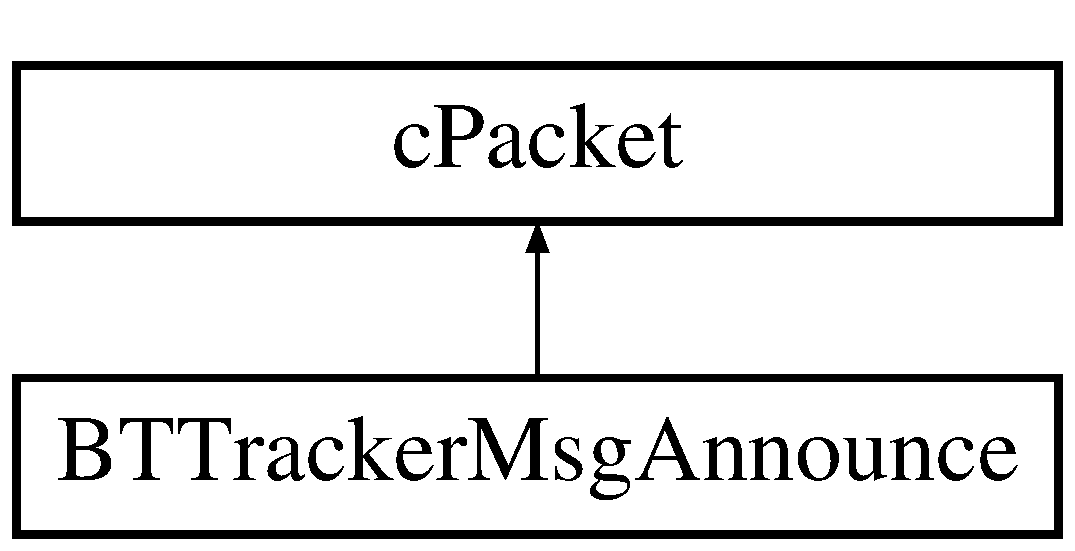
\includegraphics[height=2.000000cm]{classBTTrackerMsgAnnounce}
\end{center}
\end{figure}
\subsection*{Public Member Functions}
\begin{DoxyCompactItemize}
\item 
\hyperlink{classBTTrackerMsgAnnounce_a006351da6f99e4f73785cad49b5aecfa}{B\+T\+Tracker\+Msg\+Announce} (const char $\ast$name=N\+U\+L\+L, int kind=0)
\item 
\hyperlink{classBTTrackerMsgAnnounce_aba77a16bcb9bef02a2fdb5e2d04a9902}{B\+T\+Tracker\+Msg\+Announce} (const \hyperlink{classBTTrackerMsgAnnounce}{B\+T\+Tracker\+Msg\+Announce} \&other)
\item 
virtual \hyperlink{classBTTrackerMsgAnnounce_adaf5432a83e4311ef137e4b3260a0b22}{$\sim$\+B\+T\+Tracker\+Msg\+Announce} ()
\item 
\hyperlink{classBTTrackerMsgAnnounce}{B\+T\+Tracker\+Msg\+Announce} \& \hyperlink{classBTTrackerMsgAnnounce_ade1e515aa0cf6a0890cd6a504bae43c8}{operator=} (const \hyperlink{classBTTrackerMsgAnnounce}{B\+T\+Tracker\+Msg\+Announce} \&other)
\item 
virtual \hyperlink{classBTTrackerMsgAnnounce}{B\+T\+Tracker\+Msg\+Announce} $\ast$ \hyperlink{classBTTrackerMsgAnnounce_ae71c93192d9643deca2df1d2509abc81}{dup} () const 
\item 
virtual void \hyperlink{classBTTrackerMsgAnnounce_aff2342db405a7679f229c479c11f46b4}{parsim\+Pack} (c\+Comm\+Buffer $\ast$b)
\item 
virtual void \hyperlink{classBTTrackerMsgAnnounce_aca0e70bb2c37f8c71ade83831a7c35d3}{parsim\+Unpack} (c\+Comm\+Buffer $\ast$b)
\item 
virtual const char $\ast$ \hyperlink{classBTTrackerMsgAnnounce_ab310c662c11b529992a367a2e1b15b3c}{info\+Hash} () const 
\item 
virtual void \hyperlink{classBTTrackerMsgAnnounce_a766f9fb2b4b0679952916eadf415613f}{set\+Info\+Hash} (const char $\ast$\hyperlink{classBTTrackerMsgAnnounce_af774e44908377e324fd25e16a048c184}{info\+Hash\+\_\+var})
\item 
virtual const char $\ast$ \hyperlink{classBTTrackerMsgAnnounce_a69a230f6640baf0ea5450636e180e320}{peer\+Id} () const 
\item 
virtual void \hyperlink{classBTTrackerMsgAnnounce_ad678c6f0881dce090eeec1e4793e596e}{set\+Peer\+Id} (const char $\ast$\hyperlink{classBTTrackerMsgAnnounce_afdb278a71653823706ad6b925a03711e}{peer\+Id\+\_\+var})
\item 
virtual unsigned int \hyperlink{classBTTrackerMsgAnnounce_a9ae50e8df5acb174c65665b51f7cd3b2}{peer\+Port} () const 
\item 
virtual void \hyperlink{classBTTrackerMsgAnnounce_ab0dfd593e0377b033ffdec5673a7d303}{set\+Peer\+Port} (unsigned int \hyperlink{classBTTrackerMsgAnnounce_a8284aedb73866bde651c42c6faf6b486}{peer\+Port\+\_\+var})
\item 
virtual unsigned int \hyperlink{classBTTrackerMsgAnnounce_a1ee38ffb2e3538ab73b3fbec32b1f821}{event} () const 
\item 
virtual void \hyperlink{classBTTrackerMsgAnnounce_a018eaf9bc7c3fe9b3d8f64de6f0ba5db}{set\+Event} (unsigned int \hyperlink{classBTTrackerMsgAnnounce_acbbb1522bc659a2972e7b73eaa201df2}{event\+\_\+var})
\item 
virtual bool \hyperlink{classBTTrackerMsgAnnounce_a1196242607e513f3fb77d76f12151dd8}{compact} () const 
\item 
virtual void \hyperlink{classBTTrackerMsgAnnounce_ad07de17eb9f679db192a0a03f70f7a38}{set\+Compact} (bool \hyperlink{classBTTrackerMsgAnnounce_a22ee38ffb1718174a7684bdb13200e24}{compact\+\_\+var})
\item 
virtual bool \hyperlink{classBTTrackerMsgAnnounce_a668f4f591498f054b479d9c85a259ff5}{no\+Peer\+Id} () const 
\item 
virtual void \hyperlink{classBTTrackerMsgAnnounce_a0dcdf428a91226f9abe75242043f17a9}{set\+No\+Peer\+Id} (bool \hyperlink{classBTTrackerMsgAnnounce_a3e10bd3398780f6490f349d749e0e578}{no\+Peer\+Id\+\_\+var})
\item 
virtual unsigned int \hyperlink{classBTTrackerMsgAnnounce_a393acf80f1f1f03a74ff056d771d7a24}{num\+Want} () const 
\item 
virtual void \hyperlink{classBTTrackerMsgAnnounce_a010b11a96932c69df814d81ce574df44}{set\+Num\+Want} (unsigned int \hyperlink{classBTTrackerMsgAnnounce_a080f57e3a09c716d69410dcf0d62a705}{num\+Want\+\_\+var})
\item 
virtual const char $\ast$ \hyperlink{classBTTrackerMsgAnnounce_a8599ec1d23cb24615bfca42ef46da10d}{key} () const 
\item 
virtual void \hyperlink{classBTTrackerMsgAnnounce_a7c3251f1c32620740ca08e2e2bacf95f}{set\+Key} (const char $\ast$\hyperlink{classBTTrackerMsgAnnounce_abaf4cc9b3fd1ab417d370b72d65e5420}{key\+\_\+var})
\item 
virtual const char $\ast$ \hyperlink{classBTTrackerMsgAnnounce_a2223c19c0480131ad7085cb4d8e6fb36}{tracker\+Id} () const 
\item 
virtual void \hyperlink{classBTTrackerMsgAnnounce_acd0051984ab65138cb28204837e91a32}{set\+Tracker\+Id} (const char $\ast$\hyperlink{classBTTrackerMsgAnnounce_a1353228205f838d4de9c6e22bb2a6573}{tracker\+Id\+\_\+var})
\end{DoxyCompactItemize}
\subsection*{Protected Member Functions}
\begin{DoxyCompactItemize}
\item 
bool \hyperlink{classBTTrackerMsgAnnounce_acbea02450b6e264303f713edcaa64b97}{operator==} (const \hyperlink{classBTTrackerMsgAnnounce}{B\+T\+Tracker\+Msg\+Announce} \&)
\end{DoxyCompactItemize}
\subsection*{Protected Attributes}
\begin{DoxyCompactItemize}
\item 
opp\+\_\+string \hyperlink{classBTTrackerMsgAnnounce_af774e44908377e324fd25e16a048c184}{info\+Hash\+\_\+var}
\item 
opp\+\_\+string \hyperlink{classBTTrackerMsgAnnounce_afdb278a71653823706ad6b925a03711e}{peer\+Id\+\_\+var}
\item 
unsigned int \hyperlink{classBTTrackerMsgAnnounce_a8284aedb73866bde651c42c6faf6b486}{peer\+Port\+\_\+var}
\item 
unsigned int \hyperlink{classBTTrackerMsgAnnounce_acbbb1522bc659a2972e7b73eaa201df2}{event\+\_\+var}
\item 
bool \hyperlink{classBTTrackerMsgAnnounce_a22ee38ffb1718174a7684bdb13200e24}{compact\+\_\+var}
\item 
bool \hyperlink{classBTTrackerMsgAnnounce_a3e10bd3398780f6490f349d749e0e578}{no\+Peer\+Id\+\_\+var}
\item 
unsigned int \hyperlink{classBTTrackerMsgAnnounce_a080f57e3a09c716d69410dcf0d62a705}{num\+Want\+\_\+var}
\item 
opp\+\_\+string \hyperlink{classBTTrackerMsgAnnounce_abaf4cc9b3fd1ab417d370b72d65e5420}{key\+\_\+var}
\item 
opp\+\_\+string \hyperlink{classBTTrackerMsgAnnounce_a1353228205f838d4de9c6e22bb2a6573}{tracker\+Id\+\_\+var}
\end{DoxyCompactItemize}


\subsection{Constructor \& Destructor Documentation}
\hypertarget{classBTTrackerMsgAnnounce_a006351da6f99e4f73785cad49b5aecfa}{}\index{B\+T\+Tracker\+Msg\+Announce@{B\+T\+Tracker\+Msg\+Announce}!B\+T\+Tracker\+Msg\+Announce@{B\+T\+Tracker\+Msg\+Announce}}
\index{B\+T\+Tracker\+Msg\+Announce@{B\+T\+Tracker\+Msg\+Announce}!B\+T\+Tracker\+Msg\+Announce@{B\+T\+Tracker\+Msg\+Announce}}
\subsubsection[{B\+T\+Tracker\+Msg\+Announce(const char $\ast$name=\+N\+U\+L\+L, int kind=0)}]{\setlength{\rightskip}{0pt plus 5cm}B\+T\+Tracker\+Msg\+Announce\+::\+B\+T\+Tracker\+Msg\+Announce (
\begin{DoxyParamCaption}
\item[{const char $\ast$}]{name = {\ttfamily NULL}, }
\item[{int}]{kind = {\ttfamily 0}}
\end{DoxyParamCaption}
)}\label{classBTTrackerMsgAnnounce_a006351da6f99e4f73785cad49b5aecfa}
\hypertarget{classBTTrackerMsgAnnounce_aba77a16bcb9bef02a2fdb5e2d04a9902}{}\index{B\+T\+Tracker\+Msg\+Announce@{B\+T\+Tracker\+Msg\+Announce}!B\+T\+Tracker\+Msg\+Announce@{B\+T\+Tracker\+Msg\+Announce}}
\index{B\+T\+Tracker\+Msg\+Announce@{B\+T\+Tracker\+Msg\+Announce}!B\+T\+Tracker\+Msg\+Announce@{B\+T\+Tracker\+Msg\+Announce}}
\subsubsection[{B\+T\+Tracker\+Msg\+Announce(const B\+T\+Tracker\+Msg\+Announce \&other)}]{\setlength{\rightskip}{0pt plus 5cm}B\+T\+Tracker\+Msg\+Announce\+::\+B\+T\+Tracker\+Msg\+Announce (
\begin{DoxyParamCaption}
\item[{const {\bf B\+T\+Tracker\+Msg\+Announce} \&}]{other}
\end{DoxyParamCaption}
)}\label{classBTTrackerMsgAnnounce_aba77a16bcb9bef02a2fdb5e2d04a9902}
\hypertarget{classBTTrackerMsgAnnounce_adaf5432a83e4311ef137e4b3260a0b22}{}\index{B\+T\+Tracker\+Msg\+Announce@{B\+T\+Tracker\+Msg\+Announce}!````~B\+T\+Tracker\+Msg\+Announce@{$\sim$\+B\+T\+Tracker\+Msg\+Announce}}
\index{````~B\+T\+Tracker\+Msg\+Announce@{$\sim$\+B\+T\+Tracker\+Msg\+Announce}!B\+T\+Tracker\+Msg\+Announce@{B\+T\+Tracker\+Msg\+Announce}}
\subsubsection[{$\sim$\+B\+T\+Tracker\+Msg\+Announce()}]{\setlength{\rightskip}{0pt plus 5cm}B\+T\+Tracker\+Msg\+Announce\+::$\sim$\+B\+T\+Tracker\+Msg\+Announce (
\begin{DoxyParamCaption}
{}
\end{DoxyParamCaption}
)\hspace{0.3cm}{\ttfamily [virtual]}}\label{classBTTrackerMsgAnnounce_adaf5432a83e4311ef137e4b3260a0b22}


\subsection{Member Function Documentation}
\hypertarget{classBTTrackerMsgAnnounce_a1196242607e513f3fb77d76f12151dd8}{}\index{B\+T\+Tracker\+Msg\+Announce@{B\+T\+Tracker\+Msg\+Announce}!compact@{compact}}
\index{compact@{compact}!B\+T\+Tracker\+Msg\+Announce@{B\+T\+Tracker\+Msg\+Announce}}
\subsubsection[{compact() const }]{\setlength{\rightskip}{0pt plus 5cm}bool B\+T\+Tracker\+Msg\+Announce\+::compact (
\begin{DoxyParamCaption}
{}
\end{DoxyParamCaption}
) const\hspace{0.3cm}{\ttfamily [virtual]}}\label{classBTTrackerMsgAnnounce_a1196242607e513f3fb77d76f12151dd8}
\hypertarget{classBTTrackerMsgAnnounce_ae71c93192d9643deca2df1d2509abc81}{}\index{B\+T\+Tracker\+Msg\+Announce@{B\+T\+Tracker\+Msg\+Announce}!dup@{dup}}
\index{dup@{dup}!B\+T\+Tracker\+Msg\+Announce@{B\+T\+Tracker\+Msg\+Announce}}
\subsubsection[{dup() const }]{\setlength{\rightskip}{0pt plus 5cm}virtual {\bf B\+T\+Tracker\+Msg\+Announce}$\ast$ B\+T\+Tracker\+Msg\+Announce\+::dup (
\begin{DoxyParamCaption}
{}
\end{DoxyParamCaption}
) const\hspace{0.3cm}{\ttfamily [inline]}, {\ttfamily [virtual]}}\label{classBTTrackerMsgAnnounce_ae71c93192d9643deca2df1d2509abc81}
\hypertarget{classBTTrackerMsgAnnounce_a1ee38ffb2e3538ab73b3fbec32b1f821}{}\index{B\+T\+Tracker\+Msg\+Announce@{B\+T\+Tracker\+Msg\+Announce}!event@{event}}
\index{event@{event}!B\+T\+Tracker\+Msg\+Announce@{B\+T\+Tracker\+Msg\+Announce}}
\subsubsection[{event() const }]{\setlength{\rightskip}{0pt plus 5cm}unsigned int B\+T\+Tracker\+Msg\+Announce\+::event (
\begin{DoxyParamCaption}
{}
\end{DoxyParamCaption}
) const\hspace{0.3cm}{\ttfamily [virtual]}}\label{classBTTrackerMsgAnnounce_a1ee38ffb2e3538ab73b3fbec32b1f821}
\hypertarget{classBTTrackerMsgAnnounce_ab310c662c11b529992a367a2e1b15b3c}{}\index{B\+T\+Tracker\+Msg\+Announce@{B\+T\+Tracker\+Msg\+Announce}!info\+Hash@{info\+Hash}}
\index{info\+Hash@{info\+Hash}!B\+T\+Tracker\+Msg\+Announce@{B\+T\+Tracker\+Msg\+Announce}}
\subsubsection[{info\+Hash() const }]{\setlength{\rightskip}{0pt plus 5cm}const char $\ast$ B\+T\+Tracker\+Msg\+Announce\+::info\+Hash (
\begin{DoxyParamCaption}
{}
\end{DoxyParamCaption}
) const\hspace{0.3cm}{\ttfamily [virtual]}}\label{classBTTrackerMsgAnnounce_ab310c662c11b529992a367a2e1b15b3c}
\hypertarget{classBTTrackerMsgAnnounce_a8599ec1d23cb24615bfca42ef46da10d}{}\index{B\+T\+Tracker\+Msg\+Announce@{B\+T\+Tracker\+Msg\+Announce}!key@{key}}
\index{key@{key}!B\+T\+Tracker\+Msg\+Announce@{B\+T\+Tracker\+Msg\+Announce}}
\subsubsection[{key() const }]{\setlength{\rightskip}{0pt plus 5cm}const char $\ast$ B\+T\+Tracker\+Msg\+Announce\+::key (
\begin{DoxyParamCaption}
{}
\end{DoxyParamCaption}
) const\hspace{0.3cm}{\ttfamily [virtual]}}\label{classBTTrackerMsgAnnounce_a8599ec1d23cb24615bfca42ef46da10d}
\hypertarget{classBTTrackerMsgAnnounce_a668f4f591498f054b479d9c85a259ff5}{}\index{B\+T\+Tracker\+Msg\+Announce@{B\+T\+Tracker\+Msg\+Announce}!no\+Peer\+Id@{no\+Peer\+Id}}
\index{no\+Peer\+Id@{no\+Peer\+Id}!B\+T\+Tracker\+Msg\+Announce@{B\+T\+Tracker\+Msg\+Announce}}
\subsubsection[{no\+Peer\+Id() const }]{\setlength{\rightskip}{0pt plus 5cm}bool B\+T\+Tracker\+Msg\+Announce\+::no\+Peer\+Id (
\begin{DoxyParamCaption}
{}
\end{DoxyParamCaption}
) const\hspace{0.3cm}{\ttfamily [virtual]}}\label{classBTTrackerMsgAnnounce_a668f4f591498f054b479d9c85a259ff5}
\hypertarget{classBTTrackerMsgAnnounce_a393acf80f1f1f03a74ff056d771d7a24}{}\index{B\+T\+Tracker\+Msg\+Announce@{B\+T\+Tracker\+Msg\+Announce}!num\+Want@{num\+Want}}
\index{num\+Want@{num\+Want}!B\+T\+Tracker\+Msg\+Announce@{B\+T\+Tracker\+Msg\+Announce}}
\subsubsection[{num\+Want() const }]{\setlength{\rightskip}{0pt plus 5cm}unsigned int B\+T\+Tracker\+Msg\+Announce\+::num\+Want (
\begin{DoxyParamCaption}
{}
\end{DoxyParamCaption}
) const\hspace{0.3cm}{\ttfamily [virtual]}}\label{classBTTrackerMsgAnnounce_a393acf80f1f1f03a74ff056d771d7a24}
\hypertarget{classBTTrackerMsgAnnounce_ade1e515aa0cf6a0890cd6a504bae43c8}{}\index{B\+T\+Tracker\+Msg\+Announce@{B\+T\+Tracker\+Msg\+Announce}!operator=@{operator=}}
\index{operator=@{operator=}!B\+T\+Tracker\+Msg\+Announce@{B\+T\+Tracker\+Msg\+Announce}}
\subsubsection[{operator=(const B\+T\+Tracker\+Msg\+Announce \&other)}]{\setlength{\rightskip}{0pt plus 5cm}{\bf B\+T\+Tracker\+Msg\+Announce} \& B\+T\+Tracker\+Msg\+Announce\+::operator= (
\begin{DoxyParamCaption}
\item[{const {\bf B\+T\+Tracker\+Msg\+Announce} \&}]{other}
\end{DoxyParamCaption}
)}\label{classBTTrackerMsgAnnounce_ade1e515aa0cf6a0890cd6a504bae43c8}
\hypertarget{classBTTrackerMsgAnnounce_acbea02450b6e264303f713edcaa64b97}{}\index{B\+T\+Tracker\+Msg\+Announce@{B\+T\+Tracker\+Msg\+Announce}!operator==@{operator==}}
\index{operator==@{operator==}!B\+T\+Tracker\+Msg\+Announce@{B\+T\+Tracker\+Msg\+Announce}}
\subsubsection[{operator==(const B\+T\+Tracker\+Msg\+Announce \&)}]{\setlength{\rightskip}{0pt plus 5cm}bool B\+T\+Tracker\+Msg\+Announce\+::operator== (
\begin{DoxyParamCaption}
\item[{const {\bf B\+T\+Tracker\+Msg\+Announce} \&}]{}
\end{DoxyParamCaption}
)\hspace{0.3cm}{\ttfamily [protected]}}\label{classBTTrackerMsgAnnounce_acbea02450b6e264303f713edcaa64b97}
\hypertarget{classBTTrackerMsgAnnounce_aff2342db405a7679f229c479c11f46b4}{}\index{B\+T\+Tracker\+Msg\+Announce@{B\+T\+Tracker\+Msg\+Announce}!parsim\+Pack@{parsim\+Pack}}
\index{parsim\+Pack@{parsim\+Pack}!B\+T\+Tracker\+Msg\+Announce@{B\+T\+Tracker\+Msg\+Announce}}
\subsubsection[{parsim\+Pack(c\+Comm\+Buffer $\ast$b)}]{\setlength{\rightskip}{0pt plus 5cm}void B\+T\+Tracker\+Msg\+Announce\+::parsim\+Pack (
\begin{DoxyParamCaption}
\item[{c\+Comm\+Buffer $\ast$}]{b}
\end{DoxyParamCaption}
)\hspace{0.3cm}{\ttfamily [virtual]}}\label{classBTTrackerMsgAnnounce_aff2342db405a7679f229c479c11f46b4}
\hypertarget{classBTTrackerMsgAnnounce_aca0e70bb2c37f8c71ade83831a7c35d3}{}\index{B\+T\+Tracker\+Msg\+Announce@{B\+T\+Tracker\+Msg\+Announce}!parsim\+Unpack@{parsim\+Unpack}}
\index{parsim\+Unpack@{parsim\+Unpack}!B\+T\+Tracker\+Msg\+Announce@{B\+T\+Tracker\+Msg\+Announce}}
\subsubsection[{parsim\+Unpack(c\+Comm\+Buffer $\ast$b)}]{\setlength{\rightskip}{0pt plus 5cm}void B\+T\+Tracker\+Msg\+Announce\+::parsim\+Unpack (
\begin{DoxyParamCaption}
\item[{c\+Comm\+Buffer $\ast$}]{b}
\end{DoxyParamCaption}
)\hspace{0.3cm}{\ttfamily [virtual]}}\label{classBTTrackerMsgAnnounce_aca0e70bb2c37f8c71ade83831a7c35d3}
\hypertarget{classBTTrackerMsgAnnounce_a69a230f6640baf0ea5450636e180e320}{}\index{B\+T\+Tracker\+Msg\+Announce@{B\+T\+Tracker\+Msg\+Announce}!peer\+Id@{peer\+Id}}
\index{peer\+Id@{peer\+Id}!B\+T\+Tracker\+Msg\+Announce@{B\+T\+Tracker\+Msg\+Announce}}
\subsubsection[{peer\+Id() const }]{\setlength{\rightskip}{0pt plus 5cm}const char $\ast$ B\+T\+Tracker\+Msg\+Announce\+::peer\+Id (
\begin{DoxyParamCaption}
{}
\end{DoxyParamCaption}
) const\hspace{0.3cm}{\ttfamily [virtual]}}\label{classBTTrackerMsgAnnounce_a69a230f6640baf0ea5450636e180e320}
\hypertarget{classBTTrackerMsgAnnounce_a9ae50e8df5acb174c65665b51f7cd3b2}{}\index{B\+T\+Tracker\+Msg\+Announce@{B\+T\+Tracker\+Msg\+Announce}!peer\+Port@{peer\+Port}}
\index{peer\+Port@{peer\+Port}!B\+T\+Tracker\+Msg\+Announce@{B\+T\+Tracker\+Msg\+Announce}}
\subsubsection[{peer\+Port() const }]{\setlength{\rightskip}{0pt plus 5cm}unsigned int B\+T\+Tracker\+Msg\+Announce\+::peer\+Port (
\begin{DoxyParamCaption}
{}
\end{DoxyParamCaption}
) const\hspace{0.3cm}{\ttfamily [virtual]}}\label{classBTTrackerMsgAnnounce_a9ae50e8df5acb174c65665b51f7cd3b2}
\hypertarget{classBTTrackerMsgAnnounce_ad07de17eb9f679db192a0a03f70f7a38}{}\index{B\+T\+Tracker\+Msg\+Announce@{B\+T\+Tracker\+Msg\+Announce}!set\+Compact@{set\+Compact}}
\index{set\+Compact@{set\+Compact}!B\+T\+Tracker\+Msg\+Announce@{B\+T\+Tracker\+Msg\+Announce}}
\subsubsection[{set\+Compact(bool compact\+\_\+var)}]{\setlength{\rightskip}{0pt plus 5cm}void B\+T\+Tracker\+Msg\+Announce\+::set\+Compact (
\begin{DoxyParamCaption}
\item[{bool}]{compact\+\_\+var}
\end{DoxyParamCaption}
)\hspace{0.3cm}{\ttfamily [virtual]}}\label{classBTTrackerMsgAnnounce_ad07de17eb9f679db192a0a03f70f7a38}
\hypertarget{classBTTrackerMsgAnnounce_a018eaf9bc7c3fe9b3d8f64de6f0ba5db}{}\index{B\+T\+Tracker\+Msg\+Announce@{B\+T\+Tracker\+Msg\+Announce}!set\+Event@{set\+Event}}
\index{set\+Event@{set\+Event}!B\+T\+Tracker\+Msg\+Announce@{B\+T\+Tracker\+Msg\+Announce}}
\subsubsection[{set\+Event(unsigned int event\+\_\+var)}]{\setlength{\rightskip}{0pt plus 5cm}void B\+T\+Tracker\+Msg\+Announce\+::set\+Event (
\begin{DoxyParamCaption}
\item[{unsigned int}]{event\+\_\+var}
\end{DoxyParamCaption}
)\hspace{0.3cm}{\ttfamily [virtual]}}\label{classBTTrackerMsgAnnounce_a018eaf9bc7c3fe9b3d8f64de6f0ba5db}
\hypertarget{classBTTrackerMsgAnnounce_a766f9fb2b4b0679952916eadf415613f}{}\index{B\+T\+Tracker\+Msg\+Announce@{B\+T\+Tracker\+Msg\+Announce}!set\+Info\+Hash@{set\+Info\+Hash}}
\index{set\+Info\+Hash@{set\+Info\+Hash}!B\+T\+Tracker\+Msg\+Announce@{B\+T\+Tracker\+Msg\+Announce}}
\subsubsection[{set\+Info\+Hash(const char $\ast$info\+Hash\+\_\+var)}]{\setlength{\rightskip}{0pt plus 5cm}void B\+T\+Tracker\+Msg\+Announce\+::set\+Info\+Hash (
\begin{DoxyParamCaption}
\item[{const char $\ast$}]{info\+Hash\+\_\+var}
\end{DoxyParamCaption}
)\hspace{0.3cm}{\ttfamily [virtual]}}\label{classBTTrackerMsgAnnounce_a766f9fb2b4b0679952916eadf415613f}
\hypertarget{classBTTrackerMsgAnnounce_a7c3251f1c32620740ca08e2e2bacf95f}{}\index{B\+T\+Tracker\+Msg\+Announce@{B\+T\+Tracker\+Msg\+Announce}!set\+Key@{set\+Key}}
\index{set\+Key@{set\+Key}!B\+T\+Tracker\+Msg\+Announce@{B\+T\+Tracker\+Msg\+Announce}}
\subsubsection[{set\+Key(const char $\ast$key\+\_\+var)}]{\setlength{\rightskip}{0pt plus 5cm}void B\+T\+Tracker\+Msg\+Announce\+::set\+Key (
\begin{DoxyParamCaption}
\item[{const char $\ast$}]{key\+\_\+var}
\end{DoxyParamCaption}
)\hspace{0.3cm}{\ttfamily [virtual]}}\label{classBTTrackerMsgAnnounce_a7c3251f1c32620740ca08e2e2bacf95f}
\hypertarget{classBTTrackerMsgAnnounce_a0dcdf428a91226f9abe75242043f17a9}{}\index{B\+T\+Tracker\+Msg\+Announce@{B\+T\+Tracker\+Msg\+Announce}!set\+No\+Peer\+Id@{set\+No\+Peer\+Id}}
\index{set\+No\+Peer\+Id@{set\+No\+Peer\+Id}!B\+T\+Tracker\+Msg\+Announce@{B\+T\+Tracker\+Msg\+Announce}}
\subsubsection[{set\+No\+Peer\+Id(bool no\+Peer\+Id\+\_\+var)}]{\setlength{\rightskip}{0pt plus 5cm}void B\+T\+Tracker\+Msg\+Announce\+::set\+No\+Peer\+Id (
\begin{DoxyParamCaption}
\item[{bool}]{no\+Peer\+Id\+\_\+var}
\end{DoxyParamCaption}
)\hspace{0.3cm}{\ttfamily [virtual]}}\label{classBTTrackerMsgAnnounce_a0dcdf428a91226f9abe75242043f17a9}
\hypertarget{classBTTrackerMsgAnnounce_a010b11a96932c69df814d81ce574df44}{}\index{B\+T\+Tracker\+Msg\+Announce@{B\+T\+Tracker\+Msg\+Announce}!set\+Num\+Want@{set\+Num\+Want}}
\index{set\+Num\+Want@{set\+Num\+Want}!B\+T\+Tracker\+Msg\+Announce@{B\+T\+Tracker\+Msg\+Announce}}
\subsubsection[{set\+Num\+Want(unsigned int num\+Want\+\_\+var)}]{\setlength{\rightskip}{0pt plus 5cm}void B\+T\+Tracker\+Msg\+Announce\+::set\+Num\+Want (
\begin{DoxyParamCaption}
\item[{unsigned int}]{num\+Want\+\_\+var}
\end{DoxyParamCaption}
)\hspace{0.3cm}{\ttfamily [virtual]}}\label{classBTTrackerMsgAnnounce_a010b11a96932c69df814d81ce574df44}
\hypertarget{classBTTrackerMsgAnnounce_ad678c6f0881dce090eeec1e4793e596e}{}\index{B\+T\+Tracker\+Msg\+Announce@{B\+T\+Tracker\+Msg\+Announce}!set\+Peer\+Id@{set\+Peer\+Id}}
\index{set\+Peer\+Id@{set\+Peer\+Id}!B\+T\+Tracker\+Msg\+Announce@{B\+T\+Tracker\+Msg\+Announce}}
\subsubsection[{set\+Peer\+Id(const char $\ast$peer\+Id\+\_\+var)}]{\setlength{\rightskip}{0pt plus 5cm}void B\+T\+Tracker\+Msg\+Announce\+::set\+Peer\+Id (
\begin{DoxyParamCaption}
\item[{const char $\ast$}]{peer\+Id\+\_\+var}
\end{DoxyParamCaption}
)\hspace{0.3cm}{\ttfamily [virtual]}}\label{classBTTrackerMsgAnnounce_ad678c6f0881dce090eeec1e4793e596e}
\hypertarget{classBTTrackerMsgAnnounce_ab0dfd593e0377b033ffdec5673a7d303}{}\index{B\+T\+Tracker\+Msg\+Announce@{B\+T\+Tracker\+Msg\+Announce}!set\+Peer\+Port@{set\+Peer\+Port}}
\index{set\+Peer\+Port@{set\+Peer\+Port}!B\+T\+Tracker\+Msg\+Announce@{B\+T\+Tracker\+Msg\+Announce}}
\subsubsection[{set\+Peer\+Port(unsigned int peer\+Port\+\_\+var)}]{\setlength{\rightskip}{0pt plus 5cm}void B\+T\+Tracker\+Msg\+Announce\+::set\+Peer\+Port (
\begin{DoxyParamCaption}
\item[{unsigned int}]{peer\+Port\+\_\+var}
\end{DoxyParamCaption}
)\hspace{0.3cm}{\ttfamily [virtual]}}\label{classBTTrackerMsgAnnounce_ab0dfd593e0377b033ffdec5673a7d303}
\hypertarget{classBTTrackerMsgAnnounce_acd0051984ab65138cb28204837e91a32}{}\index{B\+T\+Tracker\+Msg\+Announce@{B\+T\+Tracker\+Msg\+Announce}!set\+Tracker\+Id@{set\+Tracker\+Id}}
\index{set\+Tracker\+Id@{set\+Tracker\+Id}!B\+T\+Tracker\+Msg\+Announce@{B\+T\+Tracker\+Msg\+Announce}}
\subsubsection[{set\+Tracker\+Id(const char $\ast$tracker\+Id\+\_\+var)}]{\setlength{\rightskip}{0pt plus 5cm}void B\+T\+Tracker\+Msg\+Announce\+::set\+Tracker\+Id (
\begin{DoxyParamCaption}
\item[{const char $\ast$}]{tracker\+Id\+\_\+var}
\end{DoxyParamCaption}
)\hspace{0.3cm}{\ttfamily [virtual]}}\label{classBTTrackerMsgAnnounce_acd0051984ab65138cb28204837e91a32}
\hypertarget{classBTTrackerMsgAnnounce_a2223c19c0480131ad7085cb4d8e6fb36}{}\index{B\+T\+Tracker\+Msg\+Announce@{B\+T\+Tracker\+Msg\+Announce}!tracker\+Id@{tracker\+Id}}
\index{tracker\+Id@{tracker\+Id}!B\+T\+Tracker\+Msg\+Announce@{B\+T\+Tracker\+Msg\+Announce}}
\subsubsection[{tracker\+Id() const }]{\setlength{\rightskip}{0pt plus 5cm}const char $\ast$ B\+T\+Tracker\+Msg\+Announce\+::tracker\+Id (
\begin{DoxyParamCaption}
{}
\end{DoxyParamCaption}
) const\hspace{0.3cm}{\ttfamily [virtual]}}\label{classBTTrackerMsgAnnounce_a2223c19c0480131ad7085cb4d8e6fb36}


\subsection{Member Data Documentation}
\hypertarget{classBTTrackerMsgAnnounce_a22ee38ffb1718174a7684bdb13200e24}{}\index{B\+T\+Tracker\+Msg\+Announce@{B\+T\+Tracker\+Msg\+Announce}!compact\+\_\+var@{compact\+\_\+var}}
\index{compact\+\_\+var@{compact\+\_\+var}!B\+T\+Tracker\+Msg\+Announce@{B\+T\+Tracker\+Msg\+Announce}}
\subsubsection[{compact\+\_\+var}]{\setlength{\rightskip}{0pt plus 5cm}bool B\+T\+Tracker\+Msg\+Announce\+::compact\+\_\+var\hspace{0.3cm}{\ttfamily [protected]}}\label{classBTTrackerMsgAnnounce_a22ee38ffb1718174a7684bdb13200e24}
\hypertarget{classBTTrackerMsgAnnounce_acbbb1522bc659a2972e7b73eaa201df2}{}\index{B\+T\+Tracker\+Msg\+Announce@{B\+T\+Tracker\+Msg\+Announce}!event\+\_\+var@{event\+\_\+var}}
\index{event\+\_\+var@{event\+\_\+var}!B\+T\+Tracker\+Msg\+Announce@{B\+T\+Tracker\+Msg\+Announce}}
\subsubsection[{event\+\_\+var}]{\setlength{\rightskip}{0pt plus 5cm}unsigned int B\+T\+Tracker\+Msg\+Announce\+::event\+\_\+var\hspace{0.3cm}{\ttfamily [protected]}}\label{classBTTrackerMsgAnnounce_acbbb1522bc659a2972e7b73eaa201df2}
\hypertarget{classBTTrackerMsgAnnounce_af774e44908377e324fd25e16a048c184}{}\index{B\+T\+Tracker\+Msg\+Announce@{B\+T\+Tracker\+Msg\+Announce}!info\+Hash\+\_\+var@{info\+Hash\+\_\+var}}
\index{info\+Hash\+\_\+var@{info\+Hash\+\_\+var}!B\+T\+Tracker\+Msg\+Announce@{B\+T\+Tracker\+Msg\+Announce}}
\subsubsection[{info\+Hash\+\_\+var}]{\setlength{\rightskip}{0pt plus 5cm}opp\+\_\+string B\+T\+Tracker\+Msg\+Announce\+::info\+Hash\+\_\+var\hspace{0.3cm}{\ttfamily [protected]}}\label{classBTTrackerMsgAnnounce_af774e44908377e324fd25e16a048c184}
\hypertarget{classBTTrackerMsgAnnounce_abaf4cc9b3fd1ab417d370b72d65e5420}{}\index{B\+T\+Tracker\+Msg\+Announce@{B\+T\+Tracker\+Msg\+Announce}!key\+\_\+var@{key\+\_\+var}}
\index{key\+\_\+var@{key\+\_\+var}!B\+T\+Tracker\+Msg\+Announce@{B\+T\+Tracker\+Msg\+Announce}}
\subsubsection[{key\+\_\+var}]{\setlength{\rightskip}{0pt plus 5cm}opp\+\_\+string B\+T\+Tracker\+Msg\+Announce\+::key\+\_\+var\hspace{0.3cm}{\ttfamily [protected]}}\label{classBTTrackerMsgAnnounce_abaf4cc9b3fd1ab417d370b72d65e5420}
\hypertarget{classBTTrackerMsgAnnounce_a3e10bd3398780f6490f349d749e0e578}{}\index{B\+T\+Tracker\+Msg\+Announce@{B\+T\+Tracker\+Msg\+Announce}!no\+Peer\+Id\+\_\+var@{no\+Peer\+Id\+\_\+var}}
\index{no\+Peer\+Id\+\_\+var@{no\+Peer\+Id\+\_\+var}!B\+T\+Tracker\+Msg\+Announce@{B\+T\+Tracker\+Msg\+Announce}}
\subsubsection[{no\+Peer\+Id\+\_\+var}]{\setlength{\rightskip}{0pt plus 5cm}bool B\+T\+Tracker\+Msg\+Announce\+::no\+Peer\+Id\+\_\+var\hspace{0.3cm}{\ttfamily [protected]}}\label{classBTTrackerMsgAnnounce_a3e10bd3398780f6490f349d749e0e578}
\hypertarget{classBTTrackerMsgAnnounce_a080f57e3a09c716d69410dcf0d62a705}{}\index{B\+T\+Tracker\+Msg\+Announce@{B\+T\+Tracker\+Msg\+Announce}!num\+Want\+\_\+var@{num\+Want\+\_\+var}}
\index{num\+Want\+\_\+var@{num\+Want\+\_\+var}!B\+T\+Tracker\+Msg\+Announce@{B\+T\+Tracker\+Msg\+Announce}}
\subsubsection[{num\+Want\+\_\+var}]{\setlength{\rightskip}{0pt plus 5cm}unsigned int B\+T\+Tracker\+Msg\+Announce\+::num\+Want\+\_\+var\hspace{0.3cm}{\ttfamily [protected]}}\label{classBTTrackerMsgAnnounce_a080f57e3a09c716d69410dcf0d62a705}
\hypertarget{classBTTrackerMsgAnnounce_afdb278a71653823706ad6b925a03711e}{}\index{B\+T\+Tracker\+Msg\+Announce@{B\+T\+Tracker\+Msg\+Announce}!peer\+Id\+\_\+var@{peer\+Id\+\_\+var}}
\index{peer\+Id\+\_\+var@{peer\+Id\+\_\+var}!B\+T\+Tracker\+Msg\+Announce@{B\+T\+Tracker\+Msg\+Announce}}
\subsubsection[{peer\+Id\+\_\+var}]{\setlength{\rightskip}{0pt plus 5cm}opp\+\_\+string B\+T\+Tracker\+Msg\+Announce\+::peer\+Id\+\_\+var\hspace{0.3cm}{\ttfamily [protected]}}\label{classBTTrackerMsgAnnounce_afdb278a71653823706ad6b925a03711e}
\hypertarget{classBTTrackerMsgAnnounce_a8284aedb73866bde651c42c6faf6b486}{}\index{B\+T\+Tracker\+Msg\+Announce@{B\+T\+Tracker\+Msg\+Announce}!peer\+Port\+\_\+var@{peer\+Port\+\_\+var}}
\index{peer\+Port\+\_\+var@{peer\+Port\+\_\+var}!B\+T\+Tracker\+Msg\+Announce@{B\+T\+Tracker\+Msg\+Announce}}
\subsubsection[{peer\+Port\+\_\+var}]{\setlength{\rightskip}{0pt plus 5cm}unsigned int B\+T\+Tracker\+Msg\+Announce\+::peer\+Port\+\_\+var\hspace{0.3cm}{\ttfamily [protected]}}\label{classBTTrackerMsgAnnounce_a8284aedb73866bde651c42c6faf6b486}
\hypertarget{classBTTrackerMsgAnnounce_a1353228205f838d4de9c6e22bb2a6573}{}\index{B\+T\+Tracker\+Msg\+Announce@{B\+T\+Tracker\+Msg\+Announce}!tracker\+Id\+\_\+var@{tracker\+Id\+\_\+var}}
\index{tracker\+Id\+\_\+var@{tracker\+Id\+\_\+var}!B\+T\+Tracker\+Msg\+Announce@{B\+T\+Tracker\+Msg\+Announce}}
\subsubsection[{tracker\+Id\+\_\+var}]{\setlength{\rightskip}{0pt plus 5cm}opp\+\_\+string B\+T\+Tracker\+Msg\+Announce\+::tracker\+Id\+\_\+var\hspace{0.3cm}{\ttfamily [protected]}}\label{classBTTrackerMsgAnnounce_a1353228205f838d4de9c6e22bb2a6573}


The documentation for this class was generated from the following files\+:\begin{DoxyCompactItemize}
\item 
\hyperlink{BTTrackerMsg__m_8h}{B\+T\+Tracker\+Msg\+\_\+m.\+h}\item 
\hyperlink{BTTrackerMsg__m_8cc}{B\+T\+Tracker\+Msg\+\_\+m.\+cc}\end{DoxyCompactItemize}

\hypertarget{classBTTrackerMsgAnnounceDescriptor}{}\section{B\+T\+Tracker\+Msg\+Announce\+Descriptor Class Reference}
\label{classBTTrackerMsgAnnounceDescriptor}\index{B\+T\+Tracker\+Msg\+Announce\+Descriptor@{B\+T\+Tracker\+Msg\+Announce\+Descriptor}}
Inheritance diagram for B\+T\+Tracker\+Msg\+Announce\+Descriptor\+:\begin{figure}[H]
\begin{center}
\leavevmode
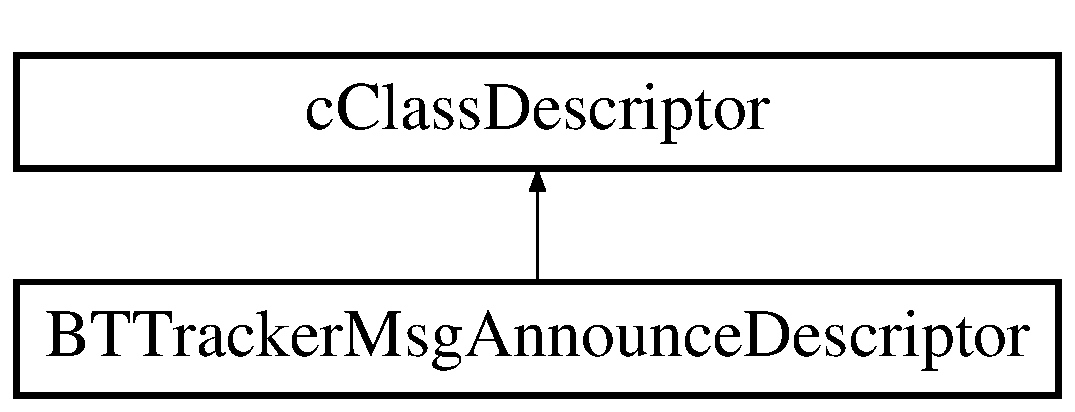
\includegraphics[height=2.000000cm]{classBTTrackerMsgAnnounceDescriptor}
\end{center}
\end{figure}
\subsection*{Public Member Functions}
\begin{DoxyCompactItemize}
\item 
\hyperlink{classBTTrackerMsgAnnounceDescriptor_ad9f6b2850a773b895519e9e1b5734b71}{B\+T\+Tracker\+Msg\+Announce\+Descriptor} ()
\item 
virtual \hyperlink{classBTTrackerMsgAnnounceDescriptor_ac35bdcd4c78dc7437bf1d6fe36deb300}{$\sim$\+B\+T\+Tracker\+Msg\+Announce\+Descriptor} ()
\item 
virtual bool \hyperlink{classBTTrackerMsgAnnounceDescriptor_ac86d66fea47ff2c466debae97dcdba00}{does\+Support} (c\+Object $\ast$obj) const 
\item 
virtual const char $\ast$ \hyperlink{classBTTrackerMsgAnnounceDescriptor_a18bcff9a777c074d3ab809c36d177678}{get\+Property} (const char $\ast$propertyname) const 
\item 
virtual int \hyperlink{classBTTrackerMsgAnnounceDescriptor_a5b4826d0b804f7fca1d144e8054403ec}{get\+Field\+Count} (void $\ast$object) const 
\item 
virtual const char $\ast$ \hyperlink{classBTTrackerMsgAnnounceDescriptor_a29addafdc451299dc8371c80269cd698}{get\+Field\+Name} (void $\ast$object, int field) const 
\item 
virtual int \hyperlink{classBTTrackerMsgAnnounceDescriptor_a17f8f695be175fe96b2c6d435bf2ab79}{find\+Field} (void $\ast$object, const char $\ast$field\+Name) const 
\item 
virtual unsigned int \hyperlink{classBTTrackerMsgAnnounceDescriptor_ab7c550be8a336bdaaf69186890501917}{get\+Field\+Type\+Flags} (void $\ast$object, int field) const 
\item 
virtual const char $\ast$ \hyperlink{classBTTrackerMsgAnnounceDescriptor_ae0dcd1e9b8855a3e2533fc21544df7a4}{get\+Field\+Type\+String} (void $\ast$object, int field) const 
\item 
virtual const char $\ast$ \hyperlink{classBTTrackerMsgAnnounceDescriptor_aae8b37cb70a1704dd2ebd1788d9f3ae9}{get\+Field\+Property} (void $\ast$object, int field, const char $\ast$propertyname) const 
\item 
virtual int \hyperlink{classBTTrackerMsgAnnounceDescriptor_a45a1e926204bddea7be6c2254364361a}{get\+Array\+Size} (void $\ast$object, int field) const 
\item 
virtual std\+::string \hyperlink{classBTTrackerMsgAnnounceDescriptor_a729bb5bb71441aee3efff6fe2ba920b5}{get\+Field\+As\+String} (void $\ast$object, int field, int i) const 
\item 
virtual bool \hyperlink{classBTTrackerMsgAnnounceDescriptor_adcc91c89a1b491ecad7a3c00539cd426}{set\+Field\+As\+String} (void $\ast$object, int field, int i, const char $\ast$value) const 
\item 
virtual const char $\ast$ \hyperlink{classBTTrackerMsgAnnounceDescriptor_a48ffbed5031cdae037fc8d762ee971b3}{get\+Field\+Struct\+Name} (void $\ast$object, int field) const 
\item 
virtual void $\ast$ \hyperlink{classBTTrackerMsgAnnounceDescriptor_a49a2a2c6d470583a79956c3ec64be7c0}{get\+Field\+Struct\+Pointer} (void $\ast$object, int field, int i) const 
\end{DoxyCompactItemize}


\subsection{Constructor \& Destructor Documentation}
\hypertarget{classBTTrackerMsgAnnounceDescriptor_ad9f6b2850a773b895519e9e1b5734b71}{}\index{B\+T\+Tracker\+Msg\+Announce\+Descriptor@{B\+T\+Tracker\+Msg\+Announce\+Descriptor}!B\+T\+Tracker\+Msg\+Announce\+Descriptor@{B\+T\+Tracker\+Msg\+Announce\+Descriptor}}
\index{B\+T\+Tracker\+Msg\+Announce\+Descriptor@{B\+T\+Tracker\+Msg\+Announce\+Descriptor}!B\+T\+Tracker\+Msg\+Announce\+Descriptor@{B\+T\+Tracker\+Msg\+Announce\+Descriptor}}
\subsubsection[{B\+T\+Tracker\+Msg\+Announce\+Descriptor()}]{\setlength{\rightskip}{0pt plus 5cm}B\+T\+Tracker\+Msg\+Announce\+Descriptor\+::\+B\+T\+Tracker\+Msg\+Announce\+Descriptor (
\begin{DoxyParamCaption}
{}
\end{DoxyParamCaption}
)}\label{classBTTrackerMsgAnnounceDescriptor_ad9f6b2850a773b895519e9e1b5734b71}
\hypertarget{classBTTrackerMsgAnnounceDescriptor_ac35bdcd4c78dc7437bf1d6fe36deb300}{}\index{B\+T\+Tracker\+Msg\+Announce\+Descriptor@{B\+T\+Tracker\+Msg\+Announce\+Descriptor}!````~B\+T\+Tracker\+Msg\+Announce\+Descriptor@{$\sim$\+B\+T\+Tracker\+Msg\+Announce\+Descriptor}}
\index{````~B\+T\+Tracker\+Msg\+Announce\+Descriptor@{$\sim$\+B\+T\+Tracker\+Msg\+Announce\+Descriptor}!B\+T\+Tracker\+Msg\+Announce\+Descriptor@{B\+T\+Tracker\+Msg\+Announce\+Descriptor}}
\subsubsection[{$\sim$\+B\+T\+Tracker\+Msg\+Announce\+Descriptor()}]{\setlength{\rightskip}{0pt plus 5cm}B\+T\+Tracker\+Msg\+Announce\+Descriptor\+::$\sim$\+B\+T\+Tracker\+Msg\+Announce\+Descriptor (
\begin{DoxyParamCaption}
{}
\end{DoxyParamCaption}
)\hspace{0.3cm}{\ttfamily [virtual]}}\label{classBTTrackerMsgAnnounceDescriptor_ac35bdcd4c78dc7437bf1d6fe36deb300}


\subsection{Member Function Documentation}
\hypertarget{classBTTrackerMsgAnnounceDescriptor_ac86d66fea47ff2c466debae97dcdba00}{}\index{B\+T\+Tracker\+Msg\+Announce\+Descriptor@{B\+T\+Tracker\+Msg\+Announce\+Descriptor}!does\+Support@{does\+Support}}
\index{does\+Support@{does\+Support}!B\+T\+Tracker\+Msg\+Announce\+Descriptor@{B\+T\+Tracker\+Msg\+Announce\+Descriptor}}
\subsubsection[{does\+Support(c\+Object $\ast$obj) const }]{\setlength{\rightskip}{0pt plus 5cm}bool B\+T\+Tracker\+Msg\+Announce\+Descriptor\+::does\+Support (
\begin{DoxyParamCaption}
\item[{c\+Object $\ast$}]{obj}
\end{DoxyParamCaption}
) const\hspace{0.3cm}{\ttfamily [virtual]}}\label{classBTTrackerMsgAnnounceDescriptor_ac86d66fea47ff2c466debae97dcdba00}
\hypertarget{classBTTrackerMsgAnnounceDescriptor_a17f8f695be175fe96b2c6d435bf2ab79}{}\index{B\+T\+Tracker\+Msg\+Announce\+Descriptor@{B\+T\+Tracker\+Msg\+Announce\+Descriptor}!find\+Field@{find\+Field}}
\index{find\+Field@{find\+Field}!B\+T\+Tracker\+Msg\+Announce\+Descriptor@{B\+T\+Tracker\+Msg\+Announce\+Descriptor}}
\subsubsection[{find\+Field(void $\ast$object, const char $\ast$field\+Name) const }]{\setlength{\rightskip}{0pt plus 5cm}int B\+T\+Tracker\+Msg\+Announce\+Descriptor\+::find\+Field (
\begin{DoxyParamCaption}
\item[{void $\ast$}]{object, }
\item[{const char $\ast$}]{field\+Name}
\end{DoxyParamCaption}
) const\hspace{0.3cm}{\ttfamily [virtual]}}\label{classBTTrackerMsgAnnounceDescriptor_a17f8f695be175fe96b2c6d435bf2ab79}
\hypertarget{classBTTrackerMsgAnnounceDescriptor_a45a1e926204bddea7be6c2254364361a}{}\index{B\+T\+Tracker\+Msg\+Announce\+Descriptor@{B\+T\+Tracker\+Msg\+Announce\+Descriptor}!get\+Array\+Size@{get\+Array\+Size}}
\index{get\+Array\+Size@{get\+Array\+Size}!B\+T\+Tracker\+Msg\+Announce\+Descriptor@{B\+T\+Tracker\+Msg\+Announce\+Descriptor}}
\subsubsection[{get\+Array\+Size(void $\ast$object, int field) const }]{\setlength{\rightskip}{0pt plus 5cm}int B\+T\+Tracker\+Msg\+Announce\+Descriptor\+::get\+Array\+Size (
\begin{DoxyParamCaption}
\item[{void $\ast$}]{object, }
\item[{int}]{field}
\end{DoxyParamCaption}
) const\hspace{0.3cm}{\ttfamily [virtual]}}\label{classBTTrackerMsgAnnounceDescriptor_a45a1e926204bddea7be6c2254364361a}
\hypertarget{classBTTrackerMsgAnnounceDescriptor_a729bb5bb71441aee3efff6fe2ba920b5}{}\index{B\+T\+Tracker\+Msg\+Announce\+Descriptor@{B\+T\+Tracker\+Msg\+Announce\+Descriptor}!get\+Field\+As\+String@{get\+Field\+As\+String}}
\index{get\+Field\+As\+String@{get\+Field\+As\+String}!B\+T\+Tracker\+Msg\+Announce\+Descriptor@{B\+T\+Tracker\+Msg\+Announce\+Descriptor}}
\subsubsection[{get\+Field\+As\+String(void $\ast$object, int field, int i) const }]{\setlength{\rightskip}{0pt plus 5cm}std\+::string B\+T\+Tracker\+Msg\+Announce\+Descriptor\+::get\+Field\+As\+String (
\begin{DoxyParamCaption}
\item[{void $\ast$}]{object, }
\item[{int}]{field, }
\item[{int}]{i}
\end{DoxyParamCaption}
) const\hspace{0.3cm}{\ttfamily [virtual]}}\label{classBTTrackerMsgAnnounceDescriptor_a729bb5bb71441aee3efff6fe2ba920b5}
\hypertarget{classBTTrackerMsgAnnounceDescriptor_a5b4826d0b804f7fca1d144e8054403ec}{}\index{B\+T\+Tracker\+Msg\+Announce\+Descriptor@{B\+T\+Tracker\+Msg\+Announce\+Descriptor}!get\+Field\+Count@{get\+Field\+Count}}
\index{get\+Field\+Count@{get\+Field\+Count}!B\+T\+Tracker\+Msg\+Announce\+Descriptor@{B\+T\+Tracker\+Msg\+Announce\+Descriptor}}
\subsubsection[{get\+Field\+Count(void $\ast$object) const }]{\setlength{\rightskip}{0pt plus 5cm}int B\+T\+Tracker\+Msg\+Announce\+Descriptor\+::get\+Field\+Count (
\begin{DoxyParamCaption}
\item[{void $\ast$}]{object}
\end{DoxyParamCaption}
) const\hspace{0.3cm}{\ttfamily [virtual]}}\label{classBTTrackerMsgAnnounceDescriptor_a5b4826d0b804f7fca1d144e8054403ec}
\hypertarget{classBTTrackerMsgAnnounceDescriptor_a29addafdc451299dc8371c80269cd698}{}\index{B\+T\+Tracker\+Msg\+Announce\+Descriptor@{B\+T\+Tracker\+Msg\+Announce\+Descriptor}!get\+Field\+Name@{get\+Field\+Name}}
\index{get\+Field\+Name@{get\+Field\+Name}!B\+T\+Tracker\+Msg\+Announce\+Descriptor@{B\+T\+Tracker\+Msg\+Announce\+Descriptor}}
\subsubsection[{get\+Field\+Name(void $\ast$object, int field) const }]{\setlength{\rightskip}{0pt plus 5cm}const char $\ast$ B\+T\+Tracker\+Msg\+Announce\+Descriptor\+::get\+Field\+Name (
\begin{DoxyParamCaption}
\item[{void $\ast$}]{object, }
\item[{int}]{field}
\end{DoxyParamCaption}
) const\hspace{0.3cm}{\ttfamily [virtual]}}\label{classBTTrackerMsgAnnounceDescriptor_a29addafdc451299dc8371c80269cd698}
\hypertarget{classBTTrackerMsgAnnounceDescriptor_aae8b37cb70a1704dd2ebd1788d9f3ae9}{}\index{B\+T\+Tracker\+Msg\+Announce\+Descriptor@{B\+T\+Tracker\+Msg\+Announce\+Descriptor}!get\+Field\+Property@{get\+Field\+Property}}
\index{get\+Field\+Property@{get\+Field\+Property}!B\+T\+Tracker\+Msg\+Announce\+Descriptor@{B\+T\+Tracker\+Msg\+Announce\+Descriptor}}
\subsubsection[{get\+Field\+Property(void $\ast$object, int field, const char $\ast$propertyname) const }]{\setlength{\rightskip}{0pt plus 5cm}const char $\ast$ B\+T\+Tracker\+Msg\+Announce\+Descriptor\+::get\+Field\+Property (
\begin{DoxyParamCaption}
\item[{void $\ast$}]{object, }
\item[{int}]{field, }
\item[{const char $\ast$}]{propertyname}
\end{DoxyParamCaption}
) const\hspace{0.3cm}{\ttfamily [virtual]}}\label{classBTTrackerMsgAnnounceDescriptor_aae8b37cb70a1704dd2ebd1788d9f3ae9}
\hypertarget{classBTTrackerMsgAnnounceDescriptor_a48ffbed5031cdae037fc8d762ee971b3}{}\index{B\+T\+Tracker\+Msg\+Announce\+Descriptor@{B\+T\+Tracker\+Msg\+Announce\+Descriptor}!get\+Field\+Struct\+Name@{get\+Field\+Struct\+Name}}
\index{get\+Field\+Struct\+Name@{get\+Field\+Struct\+Name}!B\+T\+Tracker\+Msg\+Announce\+Descriptor@{B\+T\+Tracker\+Msg\+Announce\+Descriptor}}
\subsubsection[{get\+Field\+Struct\+Name(void $\ast$object, int field) const }]{\setlength{\rightskip}{0pt plus 5cm}const char $\ast$ B\+T\+Tracker\+Msg\+Announce\+Descriptor\+::get\+Field\+Struct\+Name (
\begin{DoxyParamCaption}
\item[{void $\ast$}]{object, }
\item[{int}]{field}
\end{DoxyParamCaption}
) const\hspace{0.3cm}{\ttfamily [virtual]}}\label{classBTTrackerMsgAnnounceDescriptor_a48ffbed5031cdae037fc8d762ee971b3}
\hypertarget{classBTTrackerMsgAnnounceDescriptor_a49a2a2c6d470583a79956c3ec64be7c0}{}\index{B\+T\+Tracker\+Msg\+Announce\+Descriptor@{B\+T\+Tracker\+Msg\+Announce\+Descriptor}!get\+Field\+Struct\+Pointer@{get\+Field\+Struct\+Pointer}}
\index{get\+Field\+Struct\+Pointer@{get\+Field\+Struct\+Pointer}!B\+T\+Tracker\+Msg\+Announce\+Descriptor@{B\+T\+Tracker\+Msg\+Announce\+Descriptor}}
\subsubsection[{get\+Field\+Struct\+Pointer(void $\ast$object, int field, int i) const }]{\setlength{\rightskip}{0pt plus 5cm}void $\ast$ B\+T\+Tracker\+Msg\+Announce\+Descriptor\+::get\+Field\+Struct\+Pointer (
\begin{DoxyParamCaption}
\item[{void $\ast$}]{object, }
\item[{int}]{field, }
\item[{int}]{i}
\end{DoxyParamCaption}
) const\hspace{0.3cm}{\ttfamily [virtual]}}\label{classBTTrackerMsgAnnounceDescriptor_a49a2a2c6d470583a79956c3ec64be7c0}
\hypertarget{classBTTrackerMsgAnnounceDescriptor_ab7c550be8a336bdaaf69186890501917}{}\index{B\+T\+Tracker\+Msg\+Announce\+Descriptor@{B\+T\+Tracker\+Msg\+Announce\+Descriptor}!get\+Field\+Type\+Flags@{get\+Field\+Type\+Flags}}
\index{get\+Field\+Type\+Flags@{get\+Field\+Type\+Flags}!B\+T\+Tracker\+Msg\+Announce\+Descriptor@{B\+T\+Tracker\+Msg\+Announce\+Descriptor}}
\subsubsection[{get\+Field\+Type\+Flags(void $\ast$object, int field) const }]{\setlength{\rightskip}{0pt plus 5cm}unsigned int B\+T\+Tracker\+Msg\+Announce\+Descriptor\+::get\+Field\+Type\+Flags (
\begin{DoxyParamCaption}
\item[{void $\ast$}]{object, }
\item[{int}]{field}
\end{DoxyParamCaption}
) const\hspace{0.3cm}{\ttfamily [virtual]}}\label{classBTTrackerMsgAnnounceDescriptor_ab7c550be8a336bdaaf69186890501917}
\hypertarget{classBTTrackerMsgAnnounceDescriptor_ae0dcd1e9b8855a3e2533fc21544df7a4}{}\index{B\+T\+Tracker\+Msg\+Announce\+Descriptor@{B\+T\+Tracker\+Msg\+Announce\+Descriptor}!get\+Field\+Type\+String@{get\+Field\+Type\+String}}
\index{get\+Field\+Type\+String@{get\+Field\+Type\+String}!B\+T\+Tracker\+Msg\+Announce\+Descriptor@{B\+T\+Tracker\+Msg\+Announce\+Descriptor}}
\subsubsection[{get\+Field\+Type\+String(void $\ast$object, int field) const }]{\setlength{\rightskip}{0pt plus 5cm}const char $\ast$ B\+T\+Tracker\+Msg\+Announce\+Descriptor\+::get\+Field\+Type\+String (
\begin{DoxyParamCaption}
\item[{void $\ast$}]{object, }
\item[{int}]{field}
\end{DoxyParamCaption}
) const\hspace{0.3cm}{\ttfamily [virtual]}}\label{classBTTrackerMsgAnnounceDescriptor_ae0dcd1e9b8855a3e2533fc21544df7a4}
\hypertarget{classBTTrackerMsgAnnounceDescriptor_a18bcff9a777c074d3ab809c36d177678}{}\index{B\+T\+Tracker\+Msg\+Announce\+Descriptor@{B\+T\+Tracker\+Msg\+Announce\+Descriptor}!get\+Property@{get\+Property}}
\index{get\+Property@{get\+Property}!B\+T\+Tracker\+Msg\+Announce\+Descriptor@{B\+T\+Tracker\+Msg\+Announce\+Descriptor}}
\subsubsection[{get\+Property(const char $\ast$propertyname) const }]{\setlength{\rightskip}{0pt plus 5cm}const char $\ast$ B\+T\+Tracker\+Msg\+Announce\+Descriptor\+::get\+Property (
\begin{DoxyParamCaption}
\item[{const char $\ast$}]{propertyname}
\end{DoxyParamCaption}
) const\hspace{0.3cm}{\ttfamily [virtual]}}\label{classBTTrackerMsgAnnounceDescriptor_a18bcff9a777c074d3ab809c36d177678}
\hypertarget{classBTTrackerMsgAnnounceDescriptor_adcc91c89a1b491ecad7a3c00539cd426}{}\index{B\+T\+Tracker\+Msg\+Announce\+Descriptor@{B\+T\+Tracker\+Msg\+Announce\+Descriptor}!set\+Field\+As\+String@{set\+Field\+As\+String}}
\index{set\+Field\+As\+String@{set\+Field\+As\+String}!B\+T\+Tracker\+Msg\+Announce\+Descriptor@{B\+T\+Tracker\+Msg\+Announce\+Descriptor}}
\subsubsection[{set\+Field\+As\+String(void $\ast$object, int field, int i, const char $\ast$value) const }]{\setlength{\rightskip}{0pt plus 5cm}bool B\+T\+Tracker\+Msg\+Announce\+Descriptor\+::set\+Field\+As\+String (
\begin{DoxyParamCaption}
\item[{void $\ast$}]{object, }
\item[{int}]{field, }
\item[{int}]{i, }
\item[{const char $\ast$}]{value}
\end{DoxyParamCaption}
) const\hspace{0.3cm}{\ttfamily [virtual]}}\label{classBTTrackerMsgAnnounceDescriptor_adcc91c89a1b491ecad7a3c00539cd426}


The documentation for this class was generated from the following file\+:\begin{DoxyCompactItemize}
\item 
\hyperlink{BTTrackerMsg__m_8cc}{B\+T\+Tracker\+Msg\+\_\+m.\+cc}\end{DoxyCompactItemize}

\hypertarget{classBTTrackerMsgResponse}{}\section{B\+T\+Tracker\+Msg\+Response Class Reference}
\label{classBTTrackerMsgResponse}\index{B\+T\+Tracker\+Msg\+Response@{B\+T\+Tracker\+Msg\+Response}}


{\ttfamily \#include $<$B\+T\+Tracker\+Msg\+\_\+m.\+h$>$}

Inheritance diagram for B\+T\+Tracker\+Msg\+Response\+:\begin{figure}[H]
\begin{center}
\leavevmode
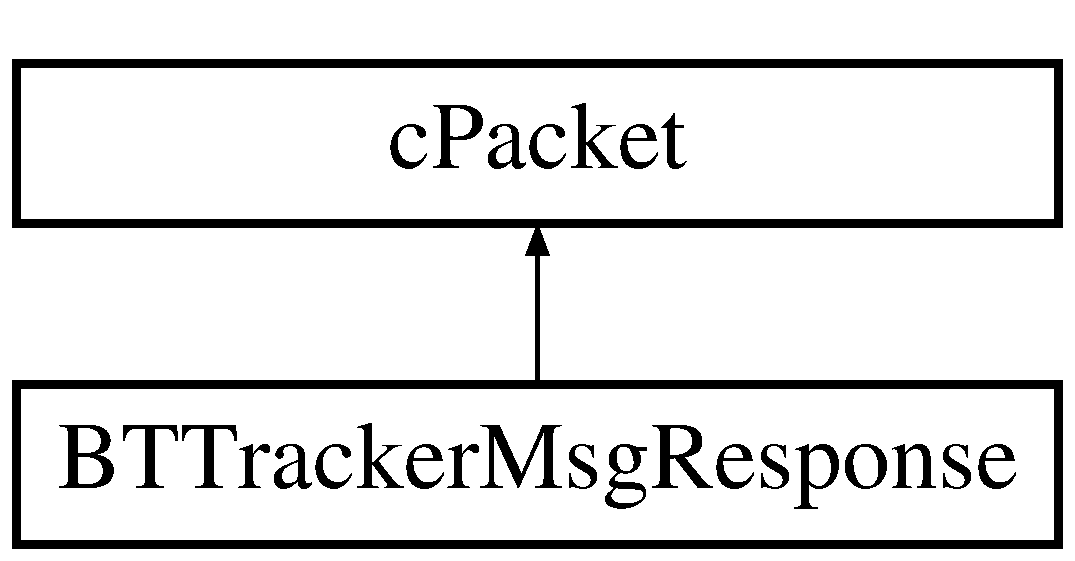
\includegraphics[height=2.000000cm]{classBTTrackerMsgResponse}
\end{center}
\end{figure}
\subsection*{Public Member Functions}
\begin{DoxyCompactItemize}
\item 
\hyperlink{classBTTrackerMsgResponse_a05ee6c15854cdba8ae16b7807232b016}{B\+T\+Tracker\+Msg\+Response} (const char $\ast$name=N\+U\+L\+L, int kind=0)
\item 
\hyperlink{classBTTrackerMsgResponse_aabeacf4915a545945a63b1f926386e0e}{B\+T\+Tracker\+Msg\+Response} (const \hyperlink{classBTTrackerMsgResponse}{B\+T\+Tracker\+Msg\+Response} \&other)
\item 
virtual \hyperlink{classBTTrackerMsgResponse_a11df55807787aaeac721254f61b85bbe}{$\sim$\+B\+T\+Tracker\+Msg\+Response} ()
\item 
\hyperlink{classBTTrackerMsgResponse}{B\+T\+Tracker\+Msg\+Response} \& \hyperlink{classBTTrackerMsgResponse_a34f2ec6fc48d6110e7846b3f0e7f4f0e}{operator=} (const \hyperlink{classBTTrackerMsgResponse}{B\+T\+Tracker\+Msg\+Response} \&other)
\item 
virtual \hyperlink{classBTTrackerMsgResponse}{B\+T\+Tracker\+Msg\+Response} $\ast$ \hyperlink{classBTTrackerMsgResponse_ac4687cbe3db1cae2e8687827852ca715}{dup} () const 
\item 
virtual void \hyperlink{classBTTrackerMsgResponse_a120681b94c04543563bdd44cb5eb0f49}{parsim\+Pack} (c\+Comm\+Buffer $\ast$b)
\item 
virtual void \hyperlink{classBTTrackerMsgResponse_af6a4a233cf072e92998d91615ab6370f}{parsim\+Unpack} (c\+Comm\+Buffer $\ast$b)
\item 
virtual const char $\ast$ \hyperlink{classBTTrackerMsgResponse_abc7ca44a791c0af1f8ad217ee18fb29d}{failure} () const 
\item 
virtual void \hyperlink{classBTTrackerMsgResponse_af306016f43f2fc54bff1ffafbaea3aac}{set\+Failure} (const char $\ast$\hyperlink{classBTTrackerMsgResponse_a0dc56a9e8c562d00690f9f72ea59b1fd}{failure\+\_\+var})
\item 
virtual const char $\ast$ \hyperlink{classBTTrackerMsgResponse_a66a8fa7e7b230667452d839b290267c9}{warning} () const 
\item 
virtual void \hyperlink{classBTTrackerMsgResponse_a5429f5a7b6bd947aa618d1d0e0e60d47}{set\+Warning} (const char $\ast$\hyperlink{classBTTrackerMsgResponse_a2d586220ffb2eb63253d19dbbce252f8}{warning\+\_\+var})
\item 
virtual unsigned int \hyperlink{classBTTrackerMsgResponse_a48954301e2cdc31321857942f9527b17}{announce\+Interval} () const 
\item 
virtual void \hyperlink{classBTTrackerMsgResponse_a124a7861f43c4fcc358889bf29720bca}{set\+Announce\+Interval} (unsigned int \hyperlink{classBTTrackerMsgResponse_a0e2fa84a47aa20e0f4a17de270b819c0}{announce\+Interval\+\_\+var})
\item 
virtual const char $\ast$ \hyperlink{classBTTrackerMsgResponse_abd9d7bcdaca8ef26dae5a28d8d08cb63}{tracker\+Id} () const 
\item 
virtual void \hyperlink{classBTTrackerMsgResponse_aaa640fe58c4c2b21e79393d597d26a26}{set\+Tracker\+Id} (const char $\ast$\hyperlink{classBTTrackerMsgResponse_a95d4eed6b7304f41ac4d967020ca5024}{tracker\+Id\+\_\+var})
\item 
virtual unsigned int \hyperlink{classBTTrackerMsgResponse_af9d26abf0691613825a557e58ccec54a}{complete} () const 
\item 
virtual void \hyperlink{classBTTrackerMsgResponse_a979ad2935b9b3cbae4fc54d9ed60c4a8}{set\+Complete} (unsigned int \hyperlink{classBTTrackerMsgResponse_a6631a0aa7c951abebf37fe5aa4ae4322}{complete\+\_\+var})
\item 
virtual unsigned int \hyperlink{classBTTrackerMsgResponse_ae0a062ad41a0d89fe1bdd17505d3f0a1}{incomplete} () const 
\item 
virtual void \hyperlink{classBTTrackerMsgResponse_aec9027a492cc165f6479841601c6c7f0}{set\+Incomplete} (unsigned int \hyperlink{classBTTrackerMsgResponse_aeec84d5b5adc2526912e05764b71fd3e}{incomplete\+\_\+var})
\item 
virtual void \hyperlink{classBTTrackerMsgResponse_a8059cb8ffd2c4bdbba6cc31e9d6b9a72}{set\+Peers\+Array\+Size} (unsigned int size)
\item 
virtual unsigned int \hyperlink{classBTTrackerMsgResponse_ad551cd9378c48865770ec0b2fa0c6874}{peers\+Array\+Size} () const 
\item 
virtual \hyperlink{structPEER}{P\+E\+E\+R} \& \hyperlink{classBTTrackerMsgResponse_aed995854e4280b5c8d1df47a07043ec1}{peers} (unsigned int k)
\item 
virtual const \hyperlink{structPEER}{P\+E\+E\+R} \& \hyperlink{classBTTrackerMsgResponse_a7bd58838c9f076780fc316e7b4972603}{peers} (unsigned int k) const 
\item 
virtual void \hyperlink{classBTTrackerMsgResponse_a11aa8270e8faf38a3605ebf55b791b95}{set\+Peers} (unsigned int k, const \hyperlink{structPEER}{P\+E\+E\+R} \&\hyperlink{classBTTrackerMsgResponse_a1aa01eb6c2c6a28498173d1d0f578b72}{peers\+\_\+var})
\end{DoxyCompactItemize}
\subsection*{Protected Member Functions}
\begin{DoxyCompactItemize}
\item 
bool \hyperlink{classBTTrackerMsgResponse_a33217d7065a2c648251407e0b61cd1a7}{operator==} (const \hyperlink{classBTTrackerMsgResponse}{B\+T\+Tracker\+Msg\+Response} \&)
\end{DoxyCompactItemize}
\subsection*{Protected Attributes}
\begin{DoxyCompactItemize}
\item 
opp\+\_\+string \hyperlink{classBTTrackerMsgResponse_a0dc56a9e8c562d00690f9f72ea59b1fd}{failure\+\_\+var}
\item 
opp\+\_\+string \hyperlink{classBTTrackerMsgResponse_a2d586220ffb2eb63253d19dbbce252f8}{warning\+\_\+var}
\item 
unsigned int \hyperlink{classBTTrackerMsgResponse_a0e2fa84a47aa20e0f4a17de270b819c0}{announce\+Interval\+\_\+var}
\item 
opp\+\_\+string \hyperlink{classBTTrackerMsgResponse_a95d4eed6b7304f41ac4d967020ca5024}{tracker\+Id\+\_\+var}
\item 
unsigned int \hyperlink{classBTTrackerMsgResponse_a6631a0aa7c951abebf37fe5aa4ae4322}{complete\+\_\+var}
\item 
unsigned int \hyperlink{classBTTrackerMsgResponse_aeec84d5b5adc2526912e05764b71fd3e}{incomplete\+\_\+var}
\item 
\+::\hyperlink{structPEER}{P\+E\+E\+R} $\ast$ \hyperlink{classBTTrackerMsgResponse_a1aa01eb6c2c6a28498173d1d0f578b72}{peers\+\_\+var}
\item 
unsigned int \hyperlink{classBTTrackerMsgResponse_a4bf054f44b6387c2d6d71d4009d96f9a}{peers\+\_\+arraysize}
\end{DoxyCompactItemize}


\subsection{Detailed Description}
Class generated from {\ttfamily applications/x\+Bit\+Torrent/\+B\+T\+Tracker\+Msg.\+msg} by opp\+\_\+msgc. 
\begin{DoxyPre}
message \hyperlink{classBTTrackerMsgResponse}{BTTrackerMsgResponse} extends cPacket
\{
    (true);\end{DoxyPre}



\begin{DoxyPre}    string failure;         
    string warning;         
    unsigned int announceInterval;  
    string trackerId;       
    unsigned int complete;      
    unsigned int incomplete;    
    \hyperlink{structPEER}{PEER} peers[];           
\}
\end{DoxyPre}
 

\subsection{Constructor \& Destructor Documentation}
\hypertarget{classBTTrackerMsgResponse_a05ee6c15854cdba8ae16b7807232b016}{}\index{B\+T\+Tracker\+Msg\+Response@{B\+T\+Tracker\+Msg\+Response}!B\+T\+Tracker\+Msg\+Response@{B\+T\+Tracker\+Msg\+Response}}
\index{B\+T\+Tracker\+Msg\+Response@{B\+T\+Tracker\+Msg\+Response}!B\+T\+Tracker\+Msg\+Response@{B\+T\+Tracker\+Msg\+Response}}
\subsubsection[{B\+T\+Tracker\+Msg\+Response(const char $\ast$name=\+N\+U\+L\+L, int kind=0)}]{\setlength{\rightskip}{0pt plus 5cm}B\+T\+Tracker\+Msg\+Response\+::\+B\+T\+Tracker\+Msg\+Response (
\begin{DoxyParamCaption}
\item[{const char $\ast$}]{name = {\ttfamily NULL}, }
\item[{int}]{kind = {\ttfamily 0}}
\end{DoxyParamCaption}
)}\label{classBTTrackerMsgResponse_a05ee6c15854cdba8ae16b7807232b016}
\hypertarget{classBTTrackerMsgResponse_aabeacf4915a545945a63b1f926386e0e}{}\index{B\+T\+Tracker\+Msg\+Response@{B\+T\+Tracker\+Msg\+Response}!B\+T\+Tracker\+Msg\+Response@{B\+T\+Tracker\+Msg\+Response}}
\index{B\+T\+Tracker\+Msg\+Response@{B\+T\+Tracker\+Msg\+Response}!B\+T\+Tracker\+Msg\+Response@{B\+T\+Tracker\+Msg\+Response}}
\subsubsection[{B\+T\+Tracker\+Msg\+Response(const B\+T\+Tracker\+Msg\+Response \&other)}]{\setlength{\rightskip}{0pt plus 5cm}B\+T\+Tracker\+Msg\+Response\+::\+B\+T\+Tracker\+Msg\+Response (
\begin{DoxyParamCaption}
\item[{const {\bf B\+T\+Tracker\+Msg\+Response} \&}]{other}
\end{DoxyParamCaption}
)}\label{classBTTrackerMsgResponse_aabeacf4915a545945a63b1f926386e0e}
\hypertarget{classBTTrackerMsgResponse_a11df55807787aaeac721254f61b85bbe}{}\index{B\+T\+Tracker\+Msg\+Response@{B\+T\+Tracker\+Msg\+Response}!````~B\+T\+Tracker\+Msg\+Response@{$\sim$\+B\+T\+Tracker\+Msg\+Response}}
\index{````~B\+T\+Tracker\+Msg\+Response@{$\sim$\+B\+T\+Tracker\+Msg\+Response}!B\+T\+Tracker\+Msg\+Response@{B\+T\+Tracker\+Msg\+Response}}
\subsubsection[{$\sim$\+B\+T\+Tracker\+Msg\+Response()}]{\setlength{\rightskip}{0pt plus 5cm}B\+T\+Tracker\+Msg\+Response\+::$\sim$\+B\+T\+Tracker\+Msg\+Response (
\begin{DoxyParamCaption}
{}
\end{DoxyParamCaption}
)\hspace{0.3cm}{\ttfamily [virtual]}}\label{classBTTrackerMsgResponse_a11df55807787aaeac721254f61b85bbe}


\subsection{Member Function Documentation}
\hypertarget{classBTTrackerMsgResponse_a48954301e2cdc31321857942f9527b17}{}\index{B\+T\+Tracker\+Msg\+Response@{B\+T\+Tracker\+Msg\+Response}!announce\+Interval@{announce\+Interval}}
\index{announce\+Interval@{announce\+Interval}!B\+T\+Tracker\+Msg\+Response@{B\+T\+Tracker\+Msg\+Response}}
\subsubsection[{announce\+Interval() const }]{\setlength{\rightskip}{0pt plus 5cm}unsigned int B\+T\+Tracker\+Msg\+Response\+::announce\+Interval (
\begin{DoxyParamCaption}
{}
\end{DoxyParamCaption}
) const\hspace{0.3cm}{\ttfamily [virtual]}}\label{classBTTrackerMsgResponse_a48954301e2cdc31321857942f9527b17}
\hypertarget{classBTTrackerMsgResponse_af9d26abf0691613825a557e58ccec54a}{}\index{B\+T\+Tracker\+Msg\+Response@{B\+T\+Tracker\+Msg\+Response}!complete@{complete}}
\index{complete@{complete}!B\+T\+Tracker\+Msg\+Response@{B\+T\+Tracker\+Msg\+Response}}
\subsubsection[{complete() const }]{\setlength{\rightskip}{0pt plus 5cm}unsigned int B\+T\+Tracker\+Msg\+Response\+::complete (
\begin{DoxyParamCaption}
{}
\end{DoxyParamCaption}
) const\hspace{0.3cm}{\ttfamily [virtual]}}\label{classBTTrackerMsgResponse_af9d26abf0691613825a557e58ccec54a}
\hypertarget{classBTTrackerMsgResponse_ac4687cbe3db1cae2e8687827852ca715}{}\index{B\+T\+Tracker\+Msg\+Response@{B\+T\+Tracker\+Msg\+Response}!dup@{dup}}
\index{dup@{dup}!B\+T\+Tracker\+Msg\+Response@{B\+T\+Tracker\+Msg\+Response}}
\subsubsection[{dup() const }]{\setlength{\rightskip}{0pt plus 5cm}virtual {\bf B\+T\+Tracker\+Msg\+Response}$\ast$ B\+T\+Tracker\+Msg\+Response\+::dup (
\begin{DoxyParamCaption}
{}
\end{DoxyParamCaption}
) const\hspace{0.3cm}{\ttfamily [inline]}, {\ttfamily [virtual]}}\label{classBTTrackerMsgResponse_ac4687cbe3db1cae2e8687827852ca715}
\hypertarget{classBTTrackerMsgResponse_abc7ca44a791c0af1f8ad217ee18fb29d}{}\index{B\+T\+Tracker\+Msg\+Response@{B\+T\+Tracker\+Msg\+Response}!failure@{failure}}
\index{failure@{failure}!B\+T\+Tracker\+Msg\+Response@{B\+T\+Tracker\+Msg\+Response}}
\subsubsection[{failure() const }]{\setlength{\rightskip}{0pt plus 5cm}const char $\ast$ B\+T\+Tracker\+Msg\+Response\+::failure (
\begin{DoxyParamCaption}
{}
\end{DoxyParamCaption}
) const\hspace{0.3cm}{\ttfamily [virtual]}}\label{classBTTrackerMsgResponse_abc7ca44a791c0af1f8ad217ee18fb29d}
\hypertarget{classBTTrackerMsgResponse_ae0a062ad41a0d89fe1bdd17505d3f0a1}{}\index{B\+T\+Tracker\+Msg\+Response@{B\+T\+Tracker\+Msg\+Response}!incomplete@{incomplete}}
\index{incomplete@{incomplete}!B\+T\+Tracker\+Msg\+Response@{B\+T\+Tracker\+Msg\+Response}}
\subsubsection[{incomplete() const }]{\setlength{\rightskip}{0pt plus 5cm}unsigned int B\+T\+Tracker\+Msg\+Response\+::incomplete (
\begin{DoxyParamCaption}
{}
\end{DoxyParamCaption}
) const\hspace{0.3cm}{\ttfamily [virtual]}}\label{classBTTrackerMsgResponse_ae0a062ad41a0d89fe1bdd17505d3f0a1}
\hypertarget{classBTTrackerMsgResponse_a34f2ec6fc48d6110e7846b3f0e7f4f0e}{}\index{B\+T\+Tracker\+Msg\+Response@{B\+T\+Tracker\+Msg\+Response}!operator=@{operator=}}
\index{operator=@{operator=}!B\+T\+Tracker\+Msg\+Response@{B\+T\+Tracker\+Msg\+Response}}
\subsubsection[{operator=(const B\+T\+Tracker\+Msg\+Response \&other)}]{\setlength{\rightskip}{0pt plus 5cm}{\bf B\+T\+Tracker\+Msg\+Response} \& B\+T\+Tracker\+Msg\+Response\+::operator= (
\begin{DoxyParamCaption}
\item[{const {\bf B\+T\+Tracker\+Msg\+Response} \&}]{other}
\end{DoxyParamCaption}
)}\label{classBTTrackerMsgResponse_a34f2ec6fc48d6110e7846b3f0e7f4f0e}
\hypertarget{classBTTrackerMsgResponse_a33217d7065a2c648251407e0b61cd1a7}{}\index{B\+T\+Tracker\+Msg\+Response@{B\+T\+Tracker\+Msg\+Response}!operator==@{operator==}}
\index{operator==@{operator==}!B\+T\+Tracker\+Msg\+Response@{B\+T\+Tracker\+Msg\+Response}}
\subsubsection[{operator==(const B\+T\+Tracker\+Msg\+Response \&)}]{\setlength{\rightskip}{0pt plus 5cm}bool B\+T\+Tracker\+Msg\+Response\+::operator== (
\begin{DoxyParamCaption}
\item[{const {\bf B\+T\+Tracker\+Msg\+Response} \&}]{}
\end{DoxyParamCaption}
)\hspace{0.3cm}{\ttfamily [protected]}}\label{classBTTrackerMsgResponse_a33217d7065a2c648251407e0b61cd1a7}
\hypertarget{classBTTrackerMsgResponse_a120681b94c04543563bdd44cb5eb0f49}{}\index{B\+T\+Tracker\+Msg\+Response@{B\+T\+Tracker\+Msg\+Response}!parsim\+Pack@{parsim\+Pack}}
\index{parsim\+Pack@{parsim\+Pack}!B\+T\+Tracker\+Msg\+Response@{B\+T\+Tracker\+Msg\+Response}}
\subsubsection[{parsim\+Pack(c\+Comm\+Buffer $\ast$b)}]{\setlength{\rightskip}{0pt plus 5cm}void B\+T\+Tracker\+Msg\+Response\+::parsim\+Pack (
\begin{DoxyParamCaption}
\item[{c\+Comm\+Buffer $\ast$}]{b}
\end{DoxyParamCaption}
)\hspace{0.3cm}{\ttfamily [virtual]}}\label{classBTTrackerMsgResponse_a120681b94c04543563bdd44cb5eb0f49}
\hypertarget{classBTTrackerMsgResponse_af6a4a233cf072e92998d91615ab6370f}{}\index{B\+T\+Tracker\+Msg\+Response@{B\+T\+Tracker\+Msg\+Response}!parsim\+Unpack@{parsim\+Unpack}}
\index{parsim\+Unpack@{parsim\+Unpack}!B\+T\+Tracker\+Msg\+Response@{B\+T\+Tracker\+Msg\+Response}}
\subsubsection[{parsim\+Unpack(c\+Comm\+Buffer $\ast$b)}]{\setlength{\rightskip}{0pt plus 5cm}void B\+T\+Tracker\+Msg\+Response\+::parsim\+Unpack (
\begin{DoxyParamCaption}
\item[{c\+Comm\+Buffer $\ast$}]{b}
\end{DoxyParamCaption}
)\hspace{0.3cm}{\ttfamily [virtual]}}\label{classBTTrackerMsgResponse_af6a4a233cf072e92998d91615ab6370f}
\hypertarget{classBTTrackerMsgResponse_aed995854e4280b5c8d1df47a07043ec1}{}\index{B\+T\+Tracker\+Msg\+Response@{B\+T\+Tracker\+Msg\+Response}!peers@{peers}}
\index{peers@{peers}!B\+T\+Tracker\+Msg\+Response@{B\+T\+Tracker\+Msg\+Response}}
\subsubsection[{peers(unsigned int k)}]{\setlength{\rightskip}{0pt plus 5cm}{\bf P\+E\+E\+R} \& B\+T\+Tracker\+Msg\+Response\+::peers (
\begin{DoxyParamCaption}
\item[{unsigned int}]{k}
\end{DoxyParamCaption}
)\hspace{0.3cm}{\ttfamily [virtual]}}\label{classBTTrackerMsgResponse_aed995854e4280b5c8d1df47a07043ec1}
\hypertarget{classBTTrackerMsgResponse_a7bd58838c9f076780fc316e7b4972603}{}\index{B\+T\+Tracker\+Msg\+Response@{B\+T\+Tracker\+Msg\+Response}!peers@{peers}}
\index{peers@{peers}!B\+T\+Tracker\+Msg\+Response@{B\+T\+Tracker\+Msg\+Response}}
\subsubsection[{peers(unsigned int k) const }]{\setlength{\rightskip}{0pt plus 5cm}virtual const {\bf P\+E\+E\+R}\& B\+T\+Tracker\+Msg\+Response\+::peers (
\begin{DoxyParamCaption}
\item[{unsigned int}]{k}
\end{DoxyParamCaption}
) const\hspace{0.3cm}{\ttfamily [inline]}, {\ttfamily [virtual]}}\label{classBTTrackerMsgResponse_a7bd58838c9f076780fc316e7b4972603}
\hypertarget{classBTTrackerMsgResponse_ad551cd9378c48865770ec0b2fa0c6874}{}\index{B\+T\+Tracker\+Msg\+Response@{B\+T\+Tracker\+Msg\+Response}!peers\+Array\+Size@{peers\+Array\+Size}}
\index{peers\+Array\+Size@{peers\+Array\+Size}!B\+T\+Tracker\+Msg\+Response@{B\+T\+Tracker\+Msg\+Response}}
\subsubsection[{peers\+Array\+Size() const }]{\setlength{\rightskip}{0pt plus 5cm}unsigned int B\+T\+Tracker\+Msg\+Response\+::peers\+Array\+Size (
\begin{DoxyParamCaption}
{}
\end{DoxyParamCaption}
) const\hspace{0.3cm}{\ttfamily [virtual]}}\label{classBTTrackerMsgResponse_ad551cd9378c48865770ec0b2fa0c6874}
\hypertarget{classBTTrackerMsgResponse_a124a7861f43c4fcc358889bf29720bca}{}\index{B\+T\+Tracker\+Msg\+Response@{B\+T\+Tracker\+Msg\+Response}!set\+Announce\+Interval@{set\+Announce\+Interval}}
\index{set\+Announce\+Interval@{set\+Announce\+Interval}!B\+T\+Tracker\+Msg\+Response@{B\+T\+Tracker\+Msg\+Response}}
\subsubsection[{set\+Announce\+Interval(unsigned int announce\+Interval\+\_\+var)}]{\setlength{\rightskip}{0pt plus 5cm}void B\+T\+Tracker\+Msg\+Response\+::set\+Announce\+Interval (
\begin{DoxyParamCaption}
\item[{unsigned int}]{announce\+Interval\+\_\+var}
\end{DoxyParamCaption}
)\hspace{0.3cm}{\ttfamily [virtual]}}\label{classBTTrackerMsgResponse_a124a7861f43c4fcc358889bf29720bca}
\hypertarget{classBTTrackerMsgResponse_a979ad2935b9b3cbae4fc54d9ed60c4a8}{}\index{B\+T\+Tracker\+Msg\+Response@{B\+T\+Tracker\+Msg\+Response}!set\+Complete@{set\+Complete}}
\index{set\+Complete@{set\+Complete}!B\+T\+Tracker\+Msg\+Response@{B\+T\+Tracker\+Msg\+Response}}
\subsubsection[{set\+Complete(unsigned int complete\+\_\+var)}]{\setlength{\rightskip}{0pt plus 5cm}void B\+T\+Tracker\+Msg\+Response\+::set\+Complete (
\begin{DoxyParamCaption}
\item[{unsigned int}]{complete\+\_\+var}
\end{DoxyParamCaption}
)\hspace{0.3cm}{\ttfamily [virtual]}}\label{classBTTrackerMsgResponse_a979ad2935b9b3cbae4fc54d9ed60c4a8}
\hypertarget{classBTTrackerMsgResponse_af306016f43f2fc54bff1ffafbaea3aac}{}\index{B\+T\+Tracker\+Msg\+Response@{B\+T\+Tracker\+Msg\+Response}!set\+Failure@{set\+Failure}}
\index{set\+Failure@{set\+Failure}!B\+T\+Tracker\+Msg\+Response@{B\+T\+Tracker\+Msg\+Response}}
\subsubsection[{set\+Failure(const char $\ast$failure\+\_\+var)}]{\setlength{\rightskip}{0pt plus 5cm}void B\+T\+Tracker\+Msg\+Response\+::set\+Failure (
\begin{DoxyParamCaption}
\item[{const char $\ast$}]{failure\+\_\+var}
\end{DoxyParamCaption}
)\hspace{0.3cm}{\ttfamily [virtual]}}\label{classBTTrackerMsgResponse_af306016f43f2fc54bff1ffafbaea3aac}
\hypertarget{classBTTrackerMsgResponse_aec9027a492cc165f6479841601c6c7f0}{}\index{B\+T\+Tracker\+Msg\+Response@{B\+T\+Tracker\+Msg\+Response}!set\+Incomplete@{set\+Incomplete}}
\index{set\+Incomplete@{set\+Incomplete}!B\+T\+Tracker\+Msg\+Response@{B\+T\+Tracker\+Msg\+Response}}
\subsubsection[{set\+Incomplete(unsigned int incomplete\+\_\+var)}]{\setlength{\rightskip}{0pt plus 5cm}void B\+T\+Tracker\+Msg\+Response\+::set\+Incomplete (
\begin{DoxyParamCaption}
\item[{unsigned int}]{incomplete\+\_\+var}
\end{DoxyParamCaption}
)\hspace{0.3cm}{\ttfamily [virtual]}}\label{classBTTrackerMsgResponse_aec9027a492cc165f6479841601c6c7f0}
\hypertarget{classBTTrackerMsgResponse_a11aa8270e8faf38a3605ebf55b791b95}{}\index{B\+T\+Tracker\+Msg\+Response@{B\+T\+Tracker\+Msg\+Response}!set\+Peers@{set\+Peers}}
\index{set\+Peers@{set\+Peers}!B\+T\+Tracker\+Msg\+Response@{B\+T\+Tracker\+Msg\+Response}}
\subsubsection[{set\+Peers(unsigned int k, const P\+E\+E\+R \&peers\+\_\+var)}]{\setlength{\rightskip}{0pt plus 5cm}void B\+T\+Tracker\+Msg\+Response\+::set\+Peers (
\begin{DoxyParamCaption}
\item[{unsigned int}]{k, }
\item[{const {\bf P\+E\+E\+R} \&}]{peers\+\_\+var}
\end{DoxyParamCaption}
)\hspace{0.3cm}{\ttfamily [virtual]}}\label{classBTTrackerMsgResponse_a11aa8270e8faf38a3605ebf55b791b95}
\hypertarget{classBTTrackerMsgResponse_a8059cb8ffd2c4bdbba6cc31e9d6b9a72}{}\index{B\+T\+Tracker\+Msg\+Response@{B\+T\+Tracker\+Msg\+Response}!set\+Peers\+Array\+Size@{set\+Peers\+Array\+Size}}
\index{set\+Peers\+Array\+Size@{set\+Peers\+Array\+Size}!B\+T\+Tracker\+Msg\+Response@{B\+T\+Tracker\+Msg\+Response}}
\subsubsection[{set\+Peers\+Array\+Size(unsigned int size)}]{\setlength{\rightskip}{0pt plus 5cm}void B\+T\+Tracker\+Msg\+Response\+::set\+Peers\+Array\+Size (
\begin{DoxyParamCaption}
\item[{unsigned int}]{size}
\end{DoxyParamCaption}
)\hspace{0.3cm}{\ttfamily [virtual]}}\label{classBTTrackerMsgResponse_a8059cb8ffd2c4bdbba6cc31e9d6b9a72}
\hypertarget{classBTTrackerMsgResponse_aaa640fe58c4c2b21e79393d597d26a26}{}\index{B\+T\+Tracker\+Msg\+Response@{B\+T\+Tracker\+Msg\+Response}!set\+Tracker\+Id@{set\+Tracker\+Id}}
\index{set\+Tracker\+Id@{set\+Tracker\+Id}!B\+T\+Tracker\+Msg\+Response@{B\+T\+Tracker\+Msg\+Response}}
\subsubsection[{set\+Tracker\+Id(const char $\ast$tracker\+Id\+\_\+var)}]{\setlength{\rightskip}{0pt plus 5cm}void B\+T\+Tracker\+Msg\+Response\+::set\+Tracker\+Id (
\begin{DoxyParamCaption}
\item[{const char $\ast$}]{tracker\+Id\+\_\+var}
\end{DoxyParamCaption}
)\hspace{0.3cm}{\ttfamily [virtual]}}\label{classBTTrackerMsgResponse_aaa640fe58c4c2b21e79393d597d26a26}
\hypertarget{classBTTrackerMsgResponse_a5429f5a7b6bd947aa618d1d0e0e60d47}{}\index{B\+T\+Tracker\+Msg\+Response@{B\+T\+Tracker\+Msg\+Response}!set\+Warning@{set\+Warning}}
\index{set\+Warning@{set\+Warning}!B\+T\+Tracker\+Msg\+Response@{B\+T\+Tracker\+Msg\+Response}}
\subsubsection[{set\+Warning(const char $\ast$warning\+\_\+var)}]{\setlength{\rightskip}{0pt plus 5cm}void B\+T\+Tracker\+Msg\+Response\+::set\+Warning (
\begin{DoxyParamCaption}
\item[{const char $\ast$}]{warning\+\_\+var}
\end{DoxyParamCaption}
)\hspace{0.3cm}{\ttfamily [virtual]}}\label{classBTTrackerMsgResponse_a5429f5a7b6bd947aa618d1d0e0e60d47}
\hypertarget{classBTTrackerMsgResponse_abd9d7bcdaca8ef26dae5a28d8d08cb63}{}\index{B\+T\+Tracker\+Msg\+Response@{B\+T\+Tracker\+Msg\+Response}!tracker\+Id@{tracker\+Id}}
\index{tracker\+Id@{tracker\+Id}!B\+T\+Tracker\+Msg\+Response@{B\+T\+Tracker\+Msg\+Response}}
\subsubsection[{tracker\+Id() const }]{\setlength{\rightskip}{0pt plus 5cm}const char $\ast$ B\+T\+Tracker\+Msg\+Response\+::tracker\+Id (
\begin{DoxyParamCaption}
{}
\end{DoxyParamCaption}
) const\hspace{0.3cm}{\ttfamily [virtual]}}\label{classBTTrackerMsgResponse_abd9d7bcdaca8ef26dae5a28d8d08cb63}
\hypertarget{classBTTrackerMsgResponse_a66a8fa7e7b230667452d839b290267c9}{}\index{B\+T\+Tracker\+Msg\+Response@{B\+T\+Tracker\+Msg\+Response}!warning@{warning}}
\index{warning@{warning}!B\+T\+Tracker\+Msg\+Response@{B\+T\+Tracker\+Msg\+Response}}
\subsubsection[{warning() const }]{\setlength{\rightskip}{0pt plus 5cm}const char $\ast$ B\+T\+Tracker\+Msg\+Response\+::warning (
\begin{DoxyParamCaption}
{}
\end{DoxyParamCaption}
) const\hspace{0.3cm}{\ttfamily [virtual]}}\label{classBTTrackerMsgResponse_a66a8fa7e7b230667452d839b290267c9}


\subsection{Member Data Documentation}
\hypertarget{classBTTrackerMsgResponse_a0e2fa84a47aa20e0f4a17de270b819c0}{}\index{B\+T\+Tracker\+Msg\+Response@{B\+T\+Tracker\+Msg\+Response}!announce\+Interval\+\_\+var@{announce\+Interval\+\_\+var}}
\index{announce\+Interval\+\_\+var@{announce\+Interval\+\_\+var}!B\+T\+Tracker\+Msg\+Response@{B\+T\+Tracker\+Msg\+Response}}
\subsubsection[{announce\+Interval\+\_\+var}]{\setlength{\rightskip}{0pt plus 5cm}unsigned int B\+T\+Tracker\+Msg\+Response\+::announce\+Interval\+\_\+var\hspace{0.3cm}{\ttfamily [protected]}}\label{classBTTrackerMsgResponse_a0e2fa84a47aa20e0f4a17de270b819c0}
\hypertarget{classBTTrackerMsgResponse_a6631a0aa7c951abebf37fe5aa4ae4322}{}\index{B\+T\+Tracker\+Msg\+Response@{B\+T\+Tracker\+Msg\+Response}!complete\+\_\+var@{complete\+\_\+var}}
\index{complete\+\_\+var@{complete\+\_\+var}!B\+T\+Tracker\+Msg\+Response@{B\+T\+Tracker\+Msg\+Response}}
\subsubsection[{complete\+\_\+var}]{\setlength{\rightskip}{0pt plus 5cm}unsigned int B\+T\+Tracker\+Msg\+Response\+::complete\+\_\+var\hspace{0.3cm}{\ttfamily [protected]}}\label{classBTTrackerMsgResponse_a6631a0aa7c951abebf37fe5aa4ae4322}
\hypertarget{classBTTrackerMsgResponse_a0dc56a9e8c562d00690f9f72ea59b1fd}{}\index{B\+T\+Tracker\+Msg\+Response@{B\+T\+Tracker\+Msg\+Response}!failure\+\_\+var@{failure\+\_\+var}}
\index{failure\+\_\+var@{failure\+\_\+var}!B\+T\+Tracker\+Msg\+Response@{B\+T\+Tracker\+Msg\+Response}}
\subsubsection[{failure\+\_\+var}]{\setlength{\rightskip}{0pt plus 5cm}opp\+\_\+string B\+T\+Tracker\+Msg\+Response\+::failure\+\_\+var\hspace{0.3cm}{\ttfamily [protected]}}\label{classBTTrackerMsgResponse_a0dc56a9e8c562d00690f9f72ea59b1fd}
\hypertarget{classBTTrackerMsgResponse_aeec84d5b5adc2526912e05764b71fd3e}{}\index{B\+T\+Tracker\+Msg\+Response@{B\+T\+Tracker\+Msg\+Response}!incomplete\+\_\+var@{incomplete\+\_\+var}}
\index{incomplete\+\_\+var@{incomplete\+\_\+var}!B\+T\+Tracker\+Msg\+Response@{B\+T\+Tracker\+Msg\+Response}}
\subsubsection[{incomplete\+\_\+var}]{\setlength{\rightskip}{0pt plus 5cm}unsigned int B\+T\+Tracker\+Msg\+Response\+::incomplete\+\_\+var\hspace{0.3cm}{\ttfamily [protected]}}\label{classBTTrackerMsgResponse_aeec84d5b5adc2526912e05764b71fd3e}
\hypertarget{classBTTrackerMsgResponse_a4bf054f44b6387c2d6d71d4009d96f9a}{}\index{B\+T\+Tracker\+Msg\+Response@{B\+T\+Tracker\+Msg\+Response}!peers\+\_\+arraysize@{peers\+\_\+arraysize}}
\index{peers\+\_\+arraysize@{peers\+\_\+arraysize}!B\+T\+Tracker\+Msg\+Response@{B\+T\+Tracker\+Msg\+Response}}
\subsubsection[{peers\+\_\+arraysize}]{\setlength{\rightskip}{0pt plus 5cm}unsigned int B\+T\+Tracker\+Msg\+Response\+::peers\+\_\+arraysize\hspace{0.3cm}{\ttfamily [protected]}}\label{classBTTrackerMsgResponse_a4bf054f44b6387c2d6d71d4009d96f9a}
\hypertarget{classBTTrackerMsgResponse_a1aa01eb6c2c6a28498173d1d0f578b72}{}\index{B\+T\+Tracker\+Msg\+Response@{B\+T\+Tracker\+Msg\+Response}!peers\+\_\+var@{peers\+\_\+var}}
\index{peers\+\_\+var@{peers\+\_\+var}!B\+T\+Tracker\+Msg\+Response@{B\+T\+Tracker\+Msg\+Response}}
\subsubsection[{peers\+\_\+var}]{\setlength{\rightskip}{0pt plus 5cm}\+::{\bf P\+E\+E\+R}$\ast$ B\+T\+Tracker\+Msg\+Response\+::peers\+\_\+var\hspace{0.3cm}{\ttfamily [protected]}}\label{classBTTrackerMsgResponse_a1aa01eb6c2c6a28498173d1d0f578b72}
\hypertarget{classBTTrackerMsgResponse_a95d4eed6b7304f41ac4d967020ca5024}{}\index{B\+T\+Tracker\+Msg\+Response@{B\+T\+Tracker\+Msg\+Response}!tracker\+Id\+\_\+var@{tracker\+Id\+\_\+var}}
\index{tracker\+Id\+\_\+var@{tracker\+Id\+\_\+var}!B\+T\+Tracker\+Msg\+Response@{B\+T\+Tracker\+Msg\+Response}}
\subsubsection[{tracker\+Id\+\_\+var}]{\setlength{\rightskip}{0pt plus 5cm}opp\+\_\+string B\+T\+Tracker\+Msg\+Response\+::tracker\+Id\+\_\+var\hspace{0.3cm}{\ttfamily [protected]}}\label{classBTTrackerMsgResponse_a95d4eed6b7304f41ac4d967020ca5024}
\hypertarget{classBTTrackerMsgResponse_a2d586220ffb2eb63253d19dbbce252f8}{}\index{B\+T\+Tracker\+Msg\+Response@{B\+T\+Tracker\+Msg\+Response}!warning\+\_\+var@{warning\+\_\+var}}
\index{warning\+\_\+var@{warning\+\_\+var}!B\+T\+Tracker\+Msg\+Response@{B\+T\+Tracker\+Msg\+Response}}
\subsubsection[{warning\+\_\+var}]{\setlength{\rightskip}{0pt plus 5cm}opp\+\_\+string B\+T\+Tracker\+Msg\+Response\+::warning\+\_\+var\hspace{0.3cm}{\ttfamily [protected]}}\label{classBTTrackerMsgResponse_a2d586220ffb2eb63253d19dbbce252f8}


The documentation for this class was generated from the following files\+:\begin{DoxyCompactItemize}
\item 
\hyperlink{BTTrackerMsg__m_8h}{B\+T\+Tracker\+Msg\+\_\+m.\+h}\item 
\hyperlink{BTTrackerMsg__m_8cc}{B\+T\+Tracker\+Msg\+\_\+m.\+cc}\end{DoxyCompactItemize}

\hypertarget{classBTTrackerMsgResponseDescriptor}{}\section{B\+T\+Tracker\+Msg\+Response\+Descriptor Class Reference}
\label{classBTTrackerMsgResponseDescriptor}\index{B\+T\+Tracker\+Msg\+Response\+Descriptor@{B\+T\+Tracker\+Msg\+Response\+Descriptor}}
Inheritance diagram for B\+T\+Tracker\+Msg\+Response\+Descriptor\+:\begin{figure}[H]
\begin{center}
\leavevmode
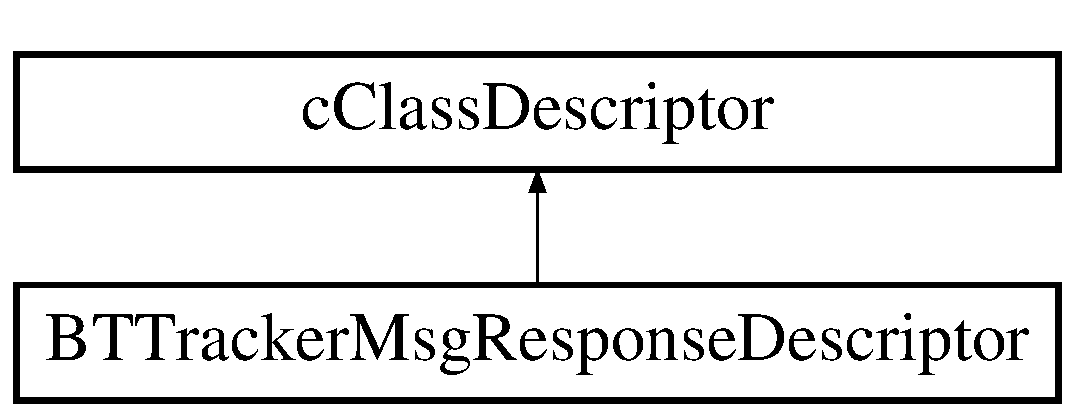
\includegraphics[height=2.000000cm]{classBTTrackerMsgResponseDescriptor}
\end{center}
\end{figure}
\subsection*{Public Member Functions}
\begin{DoxyCompactItemize}
\item 
\hyperlink{classBTTrackerMsgResponseDescriptor_a05939bc9d9af6e40c947dfbff2d8fdb7}{B\+T\+Tracker\+Msg\+Response\+Descriptor} ()
\item 
virtual \hyperlink{classBTTrackerMsgResponseDescriptor_a63db46db1fe85942d3509530d086444c}{$\sim$\+B\+T\+Tracker\+Msg\+Response\+Descriptor} ()
\item 
virtual bool \hyperlink{classBTTrackerMsgResponseDescriptor_adbd2c9bfe42a6134af457c074a8b145a}{does\+Support} (c\+Object $\ast$obj) const 
\item 
virtual const char $\ast$ \hyperlink{classBTTrackerMsgResponseDescriptor_a2e3a9360ba4a0e1337f3061ff21186ef}{get\+Property} (const char $\ast$propertyname) const 
\item 
virtual int \hyperlink{classBTTrackerMsgResponseDescriptor_a43cebef6290c4d77aaeee0cc599df9c7}{get\+Field\+Count} (void $\ast$object) const 
\item 
virtual const char $\ast$ \hyperlink{classBTTrackerMsgResponseDescriptor_a141e3bfbd0ce24dbbaac8842e5e4cdbc}{get\+Field\+Name} (void $\ast$object, int field) const 
\item 
virtual int \hyperlink{classBTTrackerMsgResponseDescriptor_ac5eb56575f8859b9ff33f7da03cee7f8}{find\+Field} (void $\ast$object, const char $\ast$field\+Name) const 
\item 
virtual unsigned int \hyperlink{classBTTrackerMsgResponseDescriptor_a280176fe000d80d350364411a4870fe6}{get\+Field\+Type\+Flags} (void $\ast$object, int field) const 
\item 
virtual const char $\ast$ \hyperlink{classBTTrackerMsgResponseDescriptor_a3c2159c41d35a6e8eb1d0d30596e0c42}{get\+Field\+Type\+String} (void $\ast$object, int field) const 
\item 
virtual const char $\ast$ \hyperlink{classBTTrackerMsgResponseDescriptor_a074e903622a2f806abe6ccd265fd0032}{get\+Field\+Property} (void $\ast$object, int field, const char $\ast$propertyname) const 
\item 
virtual int \hyperlink{classBTTrackerMsgResponseDescriptor_a07844fd76301c4cd23bed8921cf0617e}{get\+Array\+Size} (void $\ast$object, int field) const 
\item 
virtual std\+::string \hyperlink{classBTTrackerMsgResponseDescriptor_a8887ee254ea3ccfb5f659a274230952b}{get\+Field\+As\+String} (void $\ast$object, int field, int i) const 
\item 
virtual bool \hyperlink{classBTTrackerMsgResponseDescriptor_a26180e906924c6c7daf8e5c14e080fb8}{set\+Field\+As\+String} (void $\ast$object, int field, int i, const char $\ast$value) const 
\item 
virtual const char $\ast$ \hyperlink{classBTTrackerMsgResponseDescriptor_a4435ffc74501c4efcd82e40148279f59}{get\+Field\+Struct\+Name} (void $\ast$object, int field) const 
\item 
virtual void $\ast$ \hyperlink{classBTTrackerMsgResponseDescriptor_a76594b01e5f5dc7baeb01b17fce5ed3b}{get\+Field\+Struct\+Pointer} (void $\ast$object, int field, int i) const 
\end{DoxyCompactItemize}


\subsection{Constructor \& Destructor Documentation}
\hypertarget{classBTTrackerMsgResponseDescriptor_a05939bc9d9af6e40c947dfbff2d8fdb7}{}\index{B\+T\+Tracker\+Msg\+Response\+Descriptor@{B\+T\+Tracker\+Msg\+Response\+Descriptor}!B\+T\+Tracker\+Msg\+Response\+Descriptor@{B\+T\+Tracker\+Msg\+Response\+Descriptor}}
\index{B\+T\+Tracker\+Msg\+Response\+Descriptor@{B\+T\+Tracker\+Msg\+Response\+Descriptor}!B\+T\+Tracker\+Msg\+Response\+Descriptor@{B\+T\+Tracker\+Msg\+Response\+Descriptor}}
\subsubsection[{B\+T\+Tracker\+Msg\+Response\+Descriptor()}]{\setlength{\rightskip}{0pt plus 5cm}B\+T\+Tracker\+Msg\+Response\+Descriptor\+::\+B\+T\+Tracker\+Msg\+Response\+Descriptor (
\begin{DoxyParamCaption}
{}
\end{DoxyParamCaption}
)}\label{classBTTrackerMsgResponseDescriptor_a05939bc9d9af6e40c947dfbff2d8fdb7}
\hypertarget{classBTTrackerMsgResponseDescriptor_a63db46db1fe85942d3509530d086444c}{}\index{B\+T\+Tracker\+Msg\+Response\+Descriptor@{B\+T\+Tracker\+Msg\+Response\+Descriptor}!````~B\+T\+Tracker\+Msg\+Response\+Descriptor@{$\sim$\+B\+T\+Tracker\+Msg\+Response\+Descriptor}}
\index{````~B\+T\+Tracker\+Msg\+Response\+Descriptor@{$\sim$\+B\+T\+Tracker\+Msg\+Response\+Descriptor}!B\+T\+Tracker\+Msg\+Response\+Descriptor@{B\+T\+Tracker\+Msg\+Response\+Descriptor}}
\subsubsection[{$\sim$\+B\+T\+Tracker\+Msg\+Response\+Descriptor()}]{\setlength{\rightskip}{0pt plus 5cm}B\+T\+Tracker\+Msg\+Response\+Descriptor\+::$\sim$\+B\+T\+Tracker\+Msg\+Response\+Descriptor (
\begin{DoxyParamCaption}
{}
\end{DoxyParamCaption}
)\hspace{0.3cm}{\ttfamily [virtual]}}\label{classBTTrackerMsgResponseDescriptor_a63db46db1fe85942d3509530d086444c}


\subsection{Member Function Documentation}
\hypertarget{classBTTrackerMsgResponseDescriptor_adbd2c9bfe42a6134af457c074a8b145a}{}\index{B\+T\+Tracker\+Msg\+Response\+Descriptor@{B\+T\+Tracker\+Msg\+Response\+Descriptor}!does\+Support@{does\+Support}}
\index{does\+Support@{does\+Support}!B\+T\+Tracker\+Msg\+Response\+Descriptor@{B\+T\+Tracker\+Msg\+Response\+Descriptor}}
\subsubsection[{does\+Support(c\+Object $\ast$obj) const }]{\setlength{\rightskip}{0pt plus 5cm}bool B\+T\+Tracker\+Msg\+Response\+Descriptor\+::does\+Support (
\begin{DoxyParamCaption}
\item[{c\+Object $\ast$}]{obj}
\end{DoxyParamCaption}
) const\hspace{0.3cm}{\ttfamily [virtual]}}\label{classBTTrackerMsgResponseDescriptor_adbd2c9bfe42a6134af457c074a8b145a}
\hypertarget{classBTTrackerMsgResponseDescriptor_ac5eb56575f8859b9ff33f7da03cee7f8}{}\index{B\+T\+Tracker\+Msg\+Response\+Descriptor@{B\+T\+Tracker\+Msg\+Response\+Descriptor}!find\+Field@{find\+Field}}
\index{find\+Field@{find\+Field}!B\+T\+Tracker\+Msg\+Response\+Descriptor@{B\+T\+Tracker\+Msg\+Response\+Descriptor}}
\subsubsection[{find\+Field(void $\ast$object, const char $\ast$field\+Name) const }]{\setlength{\rightskip}{0pt plus 5cm}int B\+T\+Tracker\+Msg\+Response\+Descriptor\+::find\+Field (
\begin{DoxyParamCaption}
\item[{void $\ast$}]{object, }
\item[{const char $\ast$}]{field\+Name}
\end{DoxyParamCaption}
) const\hspace{0.3cm}{\ttfamily [virtual]}}\label{classBTTrackerMsgResponseDescriptor_ac5eb56575f8859b9ff33f7da03cee7f8}
\hypertarget{classBTTrackerMsgResponseDescriptor_a07844fd76301c4cd23bed8921cf0617e}{}\index{B\+T\+Tracker\+Msg\+Response\+Descriptor@{B\+T\+Tracker\+Msg\+Response\+Descriptor}!get\+Array\+Size@{get\+Array\+Size}}
\index{get\+Array\+Size@{get\+Array\+Size}!B\+T\+Tracker\+Msg\+Response\+Descriptor@{B\+T\+Tracker\+Msg\+Response\+Descriptor}}
\subsubsection[{get\+Array\+Size(void $\ast$object, int field) const }]{\setlength{\rightskip}{0pt plus 5cm}int B\+T\+Tracker\+Msg\+Response\+Descriptor\+::get\+Array\+Size (
\begin{DoxyParamCaption}
\item[{void $\ast$}]{object, }
\item[{int}]{field}
\end{DoxyParamCaption}
) const\hspace{0.3cm}{\ttfamily [virtual]}}\label{classBTTrackerMsgResponseDescriptor_a07844fd76301c4cd23bed8921cf0617e}
\hypertarget{classBTTrackerMsgResponseDescriptor_a8887ee254ea3ccfb5f659a274230952b}{}\index{B\+T\+Tracker\+Msg\+Response\+Descriptor@{B\+T\+Tracker\+Msg\+Response\+Descriptor}!get\+Field\+As\+String@{get\+Field\+As\+String}}
\index{get\+Field\+As\+String@{get\+Field\+As\+String}!B\+T\+Tracker\+Msg\+Response\+Descriptor@{B\+T\+Tracker\+Msg\+Response\+Descriptor}}
\subsubsection[{get\+Field\+As\+String(void $\ast$object, int field, int i) const }]{\setlength{\rightskip}{0pt plus 5cm}std\+::string B\+T\+Tracker\+Msg\+Response\+Descriptor\+::get\+Field\+As\+String (
\begin{DoxyParamCaption}
\item[{void $\ast$}]{object, }
\item[{int}]{field, }
\item[{int}]{i}
\end{DoxyParamCaption}
) const\hspace{0.3cm}{\ttfamily [virtual]}}\label{classBTTrackerMsgResponseDescriptor_a8887ee254ea3ccfb5f659a274230952b}
\hypertarget{classBTTrackerMsgResponseDescriptor_a43cebef6290c4d77aaeee0cc599df9c7}{}\index{B\+T\+Tracker\+Msg\+Response\+Descriptor@{B\+T\+Tracker\+Msg\+Response\+Descriptor}!get\+Field\+Count@{get\+Field\+Count}}
\index{get\+Field\+Count@{get\+Field\+Count}!B\+T\+Tracker\+Msg\+Response\+Descriptor@{B\+T\+Tracker\+Msg\+Response\+Descriptor}}
\subsubsection[{get\+Field\+Count(void $\ast$object) const }]{\setlength{\rightskip}{0pt plus 5cm}int B\+T\+Tracker\+Msg\+Response\+Descriptor\+::get\+Field\+Count (
\begin{DoxyParamCaption}
\item[{void $\ast$}]{object}
\end{DoxyParamCaption}
) const\hspace{0.3cm}{\ttfamily [virtual]}}\label{classBTTrackerMsgResponseDescriptor_a43cebef6290c4d77aaeee0cc599df9c7}
\hypertarget{classBTTrackerMsgResponseDescriptor_a141e3bfbd0ce24dbbaac8842e5e4cdbc}{}\index{B\+T\+Tracker\+Msg\+Response\+Descriptor@{B\+T\+Tracker\+Msg\+Response\+Descriptor}!get\+Field\+Name@{get\+Field\+Name}}
\index{get\+Field\+Name@{get\+Field\+Name}!B\+T\+Tracker\+Msg\+Response\+Descriptor@{B\+T\+Tracker\+Msg\+Response\+Descriptor}}
\subsubsection[{get\+Field\+Name(void $\ast$object, int field) const }]{\setlength{\rightskip}{0pt plus 5cm}const char $\ast$ B\+T\+Tracker\+Msg\+Response\+Descriptor\+::get\+Field\+Name (
\begin{DoxyParamCaption}
\item[{void $\ast$}]{object, }
\item[{int}]{field}
\end{DoxyParamCaption}
) const\hspace{0.3cm}{\ttfamily [virtual]}}\label{classBTTrackerMsgResponseDescriptor_a141e3bfbd0ce24dbbaac8842e5e4cdbc}
\hypertarget{classBTTrackerMsgResponseDescriptor_a074e903622a2f806abe6ccd265fd0032}{}\index{B\+T\+Tracker\+Msg\+Response\+Descriptor@{B\+T\+Tracker\+Msg\+Response\+Descriptor}!get\+Field\+Property@{get\+Field\+Property}}
\index{get\+Field\+Property@{get\+Field\+Property}!B\+T\+Tracker\+Msg\+Response\+Descriptor@{B\+T\+Tracker\+Msg\+Response\+Descriptor}}
\subsubsection[{get\+Field\+Property(void $\ast$object, int field, const char $\ast$propertyname) const }]{\setlength{\rightskip}{0pt plus 5cm}const char $\ast$ B\+T\+Tracker\+Msg\+Response\+Descriptor\+::get\+Field\+Property (
\begin{DoxyParamCaption}
\item[{void $\ast$}]{object, }
\item[{int}]{field, }
\item[{const char $\ast$}]{propertyname}
\end{DoxyParamCaption}
) const\hspace{0.3cm}{\ttfamily [virtual]}}\label{classBTTrackerMsgResponseDescriptor_a074e903622a2f806abe6ccd265fd0032}
\hypertarget{classBTTrackerMsgResponseDescriptor_a4435ffc74501c4efcd82e40148279f59}{}\index{B\+T\+Tracker\+Msg\+Response\+Descriptor@{B\+T\+Tracker\+Msg\+Response\+Descriptor}!get\+Field\+Struct\+Name@{get\+Field\+Struct\+Name}}
\index{get\+Field\+Struct\+Name@{get\+Field\+Struct\+Name}!B\+T\+Tracker\+Msg\+Response\+Descriptor@{B\+T\+Tracker\+Msg\+Response\+Descriptor}}
\subsubsection[{get\+Field\+Struct\+Name(void $\ast$object, int field) const }]{\setlength{\rightskip}{0pt plus 5cm}const char $\ast$ B\+T\+Tracker\+Msg\+Response\+Descriptor\+::get\+Field\+Struct\+Name (
\begin{DoxyParamCaption}
\item[{void $\ast$}]{object, }
\item[{int}]{field}
\end{DoxyParamCaption}
) const\hspace{0.3cm}{\ttfamily [virtual]}}\label{classBTTrackerMsgResponseDescriptor_a4435ffc74501c4efcd82e40148279f59}
\hypertarget{classBTTrackerMsgResponseDescriptor_a76594b01e5f5dc7baeb01b17fce5ed3b}{}\index{B\+T\+Tracker\+Msg\+Response\+Descriptor@{B\+T\+Tracker\+Msg\+Response\+Descriptor}!get\+Field\+Struct\+Pointer@{get\+Field\+Struct\+Pointer}}
\index{get\+Field\+Struct\+Pointer@{get\+Field\+Struct\+Pointer}!B\+T\+Tracker\+Msg\+Response\+Descriptor@{B\+T\+Tracker\+Msg\+Response\+Descriptor}}
\subsubsection[{get\+Field\+Struct\+Pointer(void $\ast$object, int field, int i) const }]{\setlength{\rightskip}{0pt plus 5cm}void $\ast$ B\+T\+Tracker\+Msg\+Response\+Descriptor\+::get\+Field\+Struct\+Pointer (
\begin{DoxyParamCaption}
\item[{void $\ast$}]{object, }
\item[{int}]{field, }
\item[{int}]{i}
\end{DoxyParamCaption}
) const\hspace{0.3cm}{\ttfamily [virtual]}}\label{classBTTrackerMsgResponseDescriptor_a76594b01e5f5dc7baeb01b17fce5ed3b}
\hypertarget{classBTTrackerMsgResponseDescriptor_a280176fe000d80d350364411a4870fe6}{}\index{B\+T\+Tracker\+Msg\+Response\+Descriptor@{B\+T\+Tracker\+Msg\+Response\+Descriptor}!get\+Field\+Type\+Flags@{get\+Field\+Type\+Flags}}
\index{get\+Field\+Type\+Flags@{get\+Field\+Type\+Flags}!B\+T\+Tracker\+Msg\+Response\+Descriptor@{B\+T\+Tracker\+Msg\+Response\+Descriptor}}
\subsubsection[{get\+Field\+Type\+Flags(void $\ast$object, int field) const }]{\setlength{\rightskip}{0pt plus 5cm}unsigned int B\+T\+Tracker\+Msg\+Response\+Descriptor\+::get\+Field\+Type\+Flags (
\begin{DoxyParamCaption}
\item[{void $\ast$}]{object, }
\item[{int}]{field}
\end{DoxyParamCaption}
) const\hspace{0.3cm}{\ttfamily [virtual]}}\label{classBTTrackerMsgResponseDescriptor_a280176fe000d80d350364411a4870fe6}
\hypertarget{classBTTrackerMsgResponseDescriptor_a3c2159c41d35a6e8eb1d0d30596e0c42}{}\index{B\+T\+Tracker\+Msg\+Response\+Descriptor@{B\+T\+Tracker\+Msg\+Response\+Descriptor}!get\+Field\+Type\+String@{get\+Field\+Type\+String}}
\index{get\+Field\+Type\+String@{get\+Field\+Type\+String}!B\+T\+Tracker\+Msg\+Response\+Descriptor@{B\+T\+Tracker\+Msg\+Response\+Descriptor}}
\subsubsection[{get\+Field\+Type\+String(void $\ast$object, int field) const }]{\setlength{\rightskip}{0pt plus 5cm}const char $\ast$ B\+T\+Tracker\+Msg\+Response\+Descriptor\+::get\+Field\+Type\+String (
\begin{DoxyParamCaption}
\item[{void $\ast$}]{object, }
\item[{int}]{field}
\end{DoxyParamCaption}
) const\hspace{0.3cm}{\ttfamily [virtual]}}\label{classBTTrackerMsgResponseDescriptor_a3c2159c41d35a6e8eb1d0d30596e0c42}
\hypertarget{classBTTrackerMsgResponseDescriptor_a2e3a9360ba4a0e1337f3061ff21186ef}{}\index{B\+T\+Tracker\+Msg\+Response\+Descriptor@{B\+T\+Tracker\+Msg\+Response\+Descriptor}!get\+Property@{get\+Property}}
\index{get\+Property@{get\+Property}!B\+T\+Tracker\+Msg\+Response\+Descriptor@{B\+T\+Tracker\+Msg\+Response\+Descriptor}}
\subsubsection[{get\+Property(const char $\ast$propertyname) const }]{\setlength{\rightskip}{0pt plus 5cm}const char $\ast$ B\+T\+Tracker\+Msg\+Response\+Descriptor\+::get\+Property (
\begin{DoxyParamCaption}
\item[{const char $\ast$}]{propertyname}
\end{DoxyParamCaption}
) const\hspace{0.3cm}{\ttfamily [virtual]}}\label{classBTTrackerMsgResponseDescriptor_a2e3a9360ba4a0e1337f3061ff21186ef}
\hypertarget{classBTTrackerMsgResponseDescriptor_a26180e906924c6c7daf8e5c14e080fb8}{}\index{B\+T\+Tracker\+Msg\+Response\+Descriptor@{B\+T\+Tracker\+Msg\+Response\+Descriptor}!set\+Field\+As\+String@{set\+Field\+As\+String}}
\index{set\+Field\+As\+String@{set\+Field\+As\+String}!B\+T\+Tracker\+Msg\+Response\+Descriptor@{B\+T\+Tracker\+Msg\+Response\+Descriptor}}
\subsubsection[{set\+Field\+As\+String(void $\ast$object, int field, int i, const char $\ast$value) const }]{\setlength{\rightskip}{0pt plus 5cm}bool B\+T\+Tracker\+Msg\+Response\+Descriptor\+::set\+Field\+As\+String (
\begin{DoxyParamCaption}
\item[{void $\ast$}]{object, }
\item[{int}]{field, }
\item[{int}]{i, }
\item[{const char $\ast$}]{value}
\end{DoxyParamCaption}
) const\hspace{0.3cm}{\ttfamily [virtual]}}\label{classBTTrackerMsgResponseDescriptor_a26180e906924c6c7daf8e5c14e080fb8}


The documentation for this class was generated from the following file\+:\begin{DoxyCompactItemize}
\item 
\hyperlink{BTTrackerMsg__m_8cc}{B\+T\+Tracker\+Msg\+\_\+m.\+cc}\end{DoxyCompactItemize}

\hypertarget{classBTTrackerStructBase}{}\section{B\+T\+Tracker\+Struct\+Base Class Reference}
\label{classBTTrackerStructBase}\index{B\+T\+Tracker\+Struct\+Base@{B\+T\+Tracker\+Struct\+Base}}


{\ttfamily \#include $<$B\+T\+Tracker\+Base.\+h$>$}

Inheritance diagram for B\+T\+Tracker\+Struct\+Base\+:\begin{figure}[H]
\begin{center}
\leavevmode
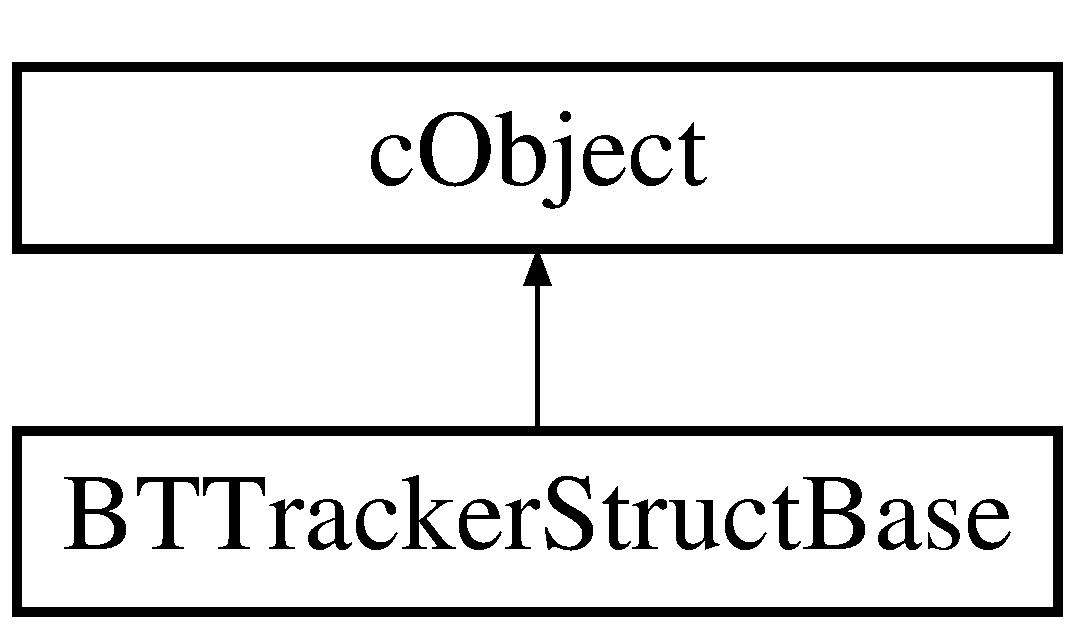
\includegraphics[height=2.000000cm]{classBTTrackerStructBase}
\end{center}
\end{figure}
\subsection*{Public Member Functions}
\begin{DoxyCompactItemize}
\item 
\hyperlink{classBTTrackerStructBase_a95263b3a44785f5ae58d4b4a8c0df889}{B\+T\+Tracker\+Struct\+Base} (const I\+Pv\+X\+Address \&, const string \&, size\+\_\+t, const string \&, simtime\+\_\+t, bool)
\item 
virtual \hyperlink{classBTTrackerStructBase_afbbc4194414fbe329ac2ffdb51e275f3}{$\sim$\+B\+T\+Tracker\+Struct\+Base} ()
\item 
bool \hyperlink{classBTTrackerStructBase_ac66964e8d8aad0678e5cf4364e99e90a}{operator==} (const \hyperlink{classBTTrackerStructBase}{B\+T\+Tracker\+Struct\+Base} \&)
\item 
const I\+Pv\+X\+Address \& \hyperlink{classBTTrackerStructBase_a98c29d3c64e02abdf592f9ad5ebc17b9}{ip\+Address} () const 
\item 
void \hyperlink{classBTTrackerStructBase_a4c2b84fb03388f33c1bfba42a14699a9}{set\+Ip\+Address} (const I\+Pv\+X\+Address \&)
\item 
const string \& \hyperlink{classBTTrackerStructBase_a93ee55a9c781903b6c2e2b665644580e}{peer\+Id} () const 
\item 
void \hyperlink{classBTTrackerStructBase_aa1df5beeeae37a93dea7b43c7c41e7a7}{set\+Peer\+Id} (const string \&)
\item 
size\+\_\+t \hyperlink{classBTTrackerStructBase_a2e453a4184d1b5ccaffbd128e3200168}{peer\+Port} () const 
\item 
void \hyperlink{classBTTrackerStructBase_a5380c7171b602657292d67f0a0644d59}{set\+Peer\+Port} (size\+\_\+t)
\item 
const string \& \hyperlink{classBTTrackerStructBase_a83ddbacdb11939b5c095e6fe8d4b3f4b}{key} () const 
\item 
void \hyperlink{classBTTrackerStructBase_a250522b23b74a585f1aaa452388db9d6}{set\+Key} (const string \&)
\item 
simtime\+\_\+t \hyperlink{classBTTrackerStructBase_a4ed22a465e65d8cea953d7a43e627c3a}{last\+Announce} () const 
\item 
void \hyperlink{classBTTrackerStructBase_ae4da4c1e130b373de29c28147c13217c}{set\+Last\+Announce} (simtime\+\_\+t)
\item 
bool \hyperlink{classBTTrackerStructBase_ad3793c0dc86881a076708bcb895d3c2d}{is\+Seed} () const 
\item 
void \hyperlink{classBTTrackerStructBase_ab7f248b9287269b8074b2cac4d377f31}{set\+Is\+Seed} (bool)
\end{DoxyCompactItemize}
\subsection*{Protected Attributes}
\begin{DoxyCompactItemize}
\item 
string \hyperlink{classBTTrackerStructBase_ae905721d92c8e64e682061215203ebde}{peer\+Id\+\_\+var}
\item 
I\+Pv\+X\+Address \hyperlink{classBTTrackerStructBase_a76d29084d65c22c38761bf8e23eb1a25}{ip\+Address\+\_\+var}
\item 
size\+\_\+t \hyperlink{classBTTrackerStructBase_ad6c17ccdd1cc1a6ae18a5d08c6eabfcc}{peer\+Port\+\_\+var}
\item 
string \hyperlink{classBTTrackerStructBase_a041ac6c48d6829f3d72c1353568e7f43}{key\+\_\+var}
\item 
simtime\+\_\+t \hyperlink{classBTTrackerStructBase_aa46de4fbdf226d5fc79df612538c2005}{last\+Announce\+\_\+var}
\item 
bool \hyperlink{classBTTrackerStructBase_a6c6788c113c4e7ba4ea28ae879bee9d7}{is\+Seed\+\_\+var}
\end{DoxyCompactItemize}


\subsection{Detailed Description}
Bit\+Torrent protocol. Implements an entry in the peers\textbackslash{}\textquotesingle{} vector. 

\subsection{Constructor \& Destructor Documentation}
\hypertarget{classBTTrackerStructBase_a95263b3a44785f5ae58d4b4a8c0df889}{}\index{B\+T\+Tracker\+Struct\+Base@{B\+T\+Tracker\+Struct\+Base}!B\+T\+Tracker\+Struct\+Base@{B\+T\+Tracker\+Struct\+Base}}
\index{B\+T\+Tracker\+Struct\+Base@{B\+T\+Tracker\+Struct\+Base}!B\+T\+Tracker\+Struct\+Base@{B\+T\+Tracker\+Struct\+Base}}
\subsubsection[{B\+T\+Tracker\+Struct\+Base(const I\+Pv\+X\+Address \&, const string \&, size\+\_\+t, const string \&, simtime\+\_\+t, bool)}]{\setlength{\rightskip}{0pt plus 5cm}B\+T\+Tracker\+Struct\+Base\+::\+B\+T\+Tracker\+Struct\+Base (
\begin{DoxyParamCaption}
\item[{const I\+Pv\+X\+Address \&}]{ip\+Address, }
\item[{const string \&}]{peer\+Id, }
\item[{size\+\_\+t}]{peer\+Port, }
\item[{const string \&}]{key, }
\item[{simtime\+\_\+t}]{last\+Announce, }
\item[{bool}]{is\+Seed}
\end{DoxyParamCaption}
)}\label{classBTTrackerStructBase_a95263b3a44785f5ae58d4b4a8c0df889}
Constructor \hypertarget{classBTTrackerStructBase_afbbc4194414fbe329ac2ffdb51e275f3}{}\index{B\+T\+Tracker\+Struct\+Base@{B\+T\+Tracker\+Struct\+Base}!````~B\+T\+Tracker\+Struct\+Base@{$\sim$\+B\+T\+Tracker\+Struct\+Base}}
\index{````~B\+T\+Tracker\+Struct\+Base@{$\sim$\+B\+T\+Tracker\+Struct\+Base}!B\+T\+Tracker\+Struct\+Base@{B\+T\+Tracker\+Struct\+Base}}
\subsubsection[{$\sim$\+B\+T\+Tracker\+Struct\+Base()}]{\setlength{\rightskip}{0pt plus 5cm}B\+T\+Tracker\+Struct\+Base\+::$\sim$\+B\+T\+Tracker\+Struct\+Base (
\begin{DoxyParamCaption}
{}
\end{DoxyParamCaption}
)\hspace{0.3cm}{\ttfamily [virtual]}}\label{classBTTrackerStructBase_afbbc4194414fbe329ac2ffdb51e275f3}
Destructor 

\subsection{Member Function Documentation}
\hypertarget{classBTTrackerStructBase_a98c29d3c64e02abdf592f9ad5ebc17b9}{}\index{B\+T\+Tracker\+Struct\+Base@{B\+T\+Tracker\+Struct\+Base}!ip\+Address@{ip\+Address}}
\index{ip\+Address@{ip\+Address}!B\+T\+Tracker\+Struct\+Base@{B\+T\+Tracker\+Struct\+Base}}
\subsubsection[{ip\+Address() const }]{\setlength{\rightskip}{0pt plus 5cm}const I\+Pv\+X\+Address \& B\+T\+Tracker\+Struct\+Base\+::ip\+Address (
\begin{DoxyParamCaption}
{}
\end{DoxyParamCaption}
) const}\label{classBTTrackerStructBase_a98c29d3c64e02abdf592f9ad5ebc17b9}
Get the I\+P address. \hypertarget{classBTTrackerStructBase_ad3793c0dc86881a076708bcb895d3c2d}{}\index{B\+T\+Tracker\+Struct\+Base@{B\+T\+Tracker\+Struct\+Base}!is\+Seed@{is\+Seed}}
\index{is\+Seed@{is\+Seed}!B\+T\+Tracker\+Struct\+Base@{B\+T\+Tracker\+Struct\+Base}}
\subsubsection[{is\+Seed() const }]{\setlength{\rightskip}{0pt plus 5cm}bool B\+T\+Tracker\+Struct\+Base\+::is\+Seed (
\begin{DoxyParamCaption}
{}
\end{DoxyParamCaption}
) const}\label{classBTTrackerStructBase_ad3793c0dc86881a076708bcb895d3c2d}
Get the value of the is\+Seed flag. \hypertarget{classBTTrackerStructBase_a83ddbacdb11939b5c095e6fe8d4b3f4b}{}\index{B\+T\+Tracker\+Struct\+Base@{B\+T\+Tracker\+Struct\+Base}!key@{key}}
\index{key@{key}!B\+T\+Tracker\+Struct\+Base@{B\+T\+Tracker\+Struct\+Base}}
\subsubsection[{key() const }]{\setlength{\rightskip}{0pt plus 5cm}const string \& B\+T\+Tracker\+Struct\+Base\+::key (
\begin{DoxyParamCaption}
{}
\end{DoxyParamCaption}
) const}\label{classBTTrackerStructBase_a83ddbacdb11939b5c095e6fe8d4b3f4b}
Get the key. \hypertarget{classBTTrackerStructBase_a4ed22a465e65d8cea953d7a43e627c3a}{}\index{B\+T\+Tracker\+Struct\+Base@{B\+T\+Tracker\+Struct\+Base}!last\+Announce@{last\+Announce}}
\index{last\+Announce@{last\+Announce}!B\+T\+Tracker\+Struct\+Base@{B\+T\+Tracker\+Struct\+Base}}
\subsubsection[{last\+Announce() const }]{\setlength{\rightskip}{0pt plus 5cm}simtime\+\_\+t B\+T\+Tracker\+Struct\+Base\+::last\+Announce (
\begin{DoxyParamCaption}
{}
\end{DoxyParamCaption}
) const}\label{classBTTrackerStructBase_a4ed22a465e65d8cea953d7a43e627c3a}
Get the last announce. \hypertarget{classBTTrackerStructBase_ac66964e8d8aad0678e5cf4364e99e90a}{}\index{B\+T\+Tracker\+Struct\+Base@{B\+T\+Tracker\+Struct\+Base}!operator==@{operator==}}
\index{operator==@{operator==}!B\+T\+Tracker\+Struct\+Base@{B\+T\+Tracker\+Struct\+Base}}
\subsubsection[{operator==(const B\+T\+Tracker\+Struct\+Base \&)}]{\setlength{\rightskip}{0pt plus 5cm}bool B\+T\+Tracker\+Struct\+Base\+::operator== (
\begin{DoxyParamCaption}
\item[{const {\bf B\+T\+Tracker\+Struct\+Base} \&}]{rhs}
\end{DoxyParamCaption}
)}\label{classBTTrackerStructBase_ac66964e8d8aad0678e5cf4364e99e90a}
Operator ==. Two entries are considered equal if the have the same key or if they have the same I\+P address and peer id. \hypertarget{classBTTrackerStructBase_a93ee55a9c781903b6c2e2b665644580e}{}\index{B\+T\+Tracker\+Struct\+Base@{B\+T\+Tracker\+Struct\+Base}!peer\+Id@{peer\+Id}}
\index{peer\+Id@{peer\+Id}!B\+T\+Tracker\+Struct\+Base@{B\+T\+Tracker\+Struct\+Base}}
\subsubsection[{peer\+Id() const }]{\setlength{\rightskip}{0pt plus 5cm}const string \& B\+T\+Tracker\+Struct\+Base\+::peer\+Id (
\begin{DoxyParamCaption}
{}
\end{DoxyParamCaption}
) const}\label{classBTTrackerStructBase_a93ee55a9c781903b6c2e2b665644580e}
Get the peer id. \hypertarget{classBTTrackerStructBase_a2e453a4184d1b5ccaffbd128e3200168}{}\index{B\+T\+Tracker\+Struct\+Base@{B\+T\+Tracker\+Struct\+Base}!peer\+Port@{peer\+Port}}
\index{peer\+Port@{peer\+Port}!B\+T\+Tracker\+Struct\+Base@{B\+T\+Tracker\+Struct\+Base}}
\subsubsection[{peer\+Port() const }]{\setlength{\rightskip}{0pt plus 5cm}size\+\_\+t B\+T\+Tracker\+Struct\+Base\+::peer\+Port (
\begin{DoxyParamCaption}
{}
\end{DoxyParamCaption}
) const}\label{classBTTrackerStructBase_a2e453a4184d1b5ccaffbd128e3200168}
Get the peer port. \hypertarget{classBTTrackerStructBase_a4c2b84fb03388f33c1bfba42a14699a9}{}\index{B\+T\+Tracker\+Struct\+Base@{B\+T\+Tracker\+Struct\+Base}!set\+Ip\+Address@{set\+Ip\+Address}}
\index{set\+Ip\+Address@{set\+Ip\+Address}!B\+T\+Tracker\+Struct\+Base@{B\+T\+Tracker\+Struct\+Base}}
\subsubsection[{set\+Ip\+Address(const I\+Pv\+X\+Address \&)}]{\setlength{\rightskip}{0pt plus 5cm}void B\+T\+Tracker\+Struct\+Base\+::set\+Ip\+Address (
\begin{DoxyParamCaption}
\item[{const I\+Pv\+X\+Address \&}]{ip\+Address}
\end{DoxyParamCaption}
)}\label{classBTTrackerStructBase_a4c2b84fb03388f33c1bfba42a14699a9}
Set the I\+P address. \hypertarget{classBTTrackerStructBase_ab7f248b9287269b8074b2cac4d377f31}{}\index{B\+T\+Tracker\+Struct\+Base@{B\+T\+Tracker\+Struct\+Base}!set\+Is\+Seed@{set\+Is\+Seed}}
\index{set\+Is\+Seed@{set\+Is\+Seed}!B\+T\+Tracker\+Struct\+Base@{B\+T\+Tracker\+Struct\+Base}}
\subsubsection[{set\+Is\+Seed(bool)}]{\setlength{\rightskip}{0pt plus 5cm}void B\+T\+Tracker\+Struct\+Base\+::set\+Is\+Seed (
\begin{DoxyParamCaption}
\item[{bool}]{is\+Seed}
\end{DoxyParamCaption}
)}\label{classBTTrackerStructBase_ab7f248b9287269b8074b2cac4d377f31}
Set the value of the is\+Seed flag. \hypertarget{classBTTrackerStructBase_a250522b23b74a585f1aaa452388db9d6}{}\index{B\+T\+Tracker\+Struct\+Base@{B\+T\+Tracker\+Struct\+Base}!set\+Key@{set\+Key}}
\index{set\+Key@{set\+Key}!B\+T\+Tracker\+Struct\+Base@{B\+T\+Tracker\+Struct\+Base}}
\subsubsection[{set\+Key(const string \&)}]{\setlength{\rightskip}{0pt plus 5cm}void B\+T\+Tracker\+Struct\+Base\+::set\+Key (
\begin{DoxyParamCaption}
\item[{const string \&}]{key}
\end{DoxyParamCaption}
)}\label{classBTTrackerStructBase_a250522b23b74a585f1aaa452388db9d6}
Set the key. \hypertarget{classBTTrackerStructBase_ae4da4c1e130b373de29c28147c13217c}{}\index{B\+T\+Tracker\+Struct\+Base@{B\+T\+Tracker\+Struct\+Base}!set\+Last\+Announce@{set\+Last\+Announce}}
\index{set\+Last\+Announce@{set\+Last\+Announce}!B\+T\+Tracker\+Struct\+Base@{B\+T\+Tracker\+Struct\+Base}}
\subsubsection[{set\+Last\+Announce(simtime\+\_\+t)}]{\setlength{\rightskip}{0pt plus 5cm}void B\+T\+Tracker\+Struct\+Base\+::set\+Last\+Announce (
\begin{DoxyParamCaption}
\item[{simtime\+\_\+t}]{last\+Announce}
\end{DoxyParamCaption}
)}\label{classBTTrackerStructBase_ae4da4c1e130b373de29c28147c13217c}
Set the last announce. \hypertarget{classBTTrackerStructBase_aa1df5beeeae37a93dea7b43c7c41e7a7}{}\index{B\+T\+Tracker\+Struct\+Base@{B\+T\+Tracker\+Struct\+Base}!set\+Peer\+Id@{set\+Peer\+Id}}
\index{set\+Peer\+Id@{set\+Peer\+Id}!B\+T\+Tracker\+Struct\+Base@{B\+T\+Tracker\+Struct\+Base}}
\subsubsection[{set\+Peer\+Id(const string \&)}]{\setlength{\rightskip}{0pt plus 5cm}void B\+T\+Tracker\+Struct\+Base\+::set\+Peer\+Id (
\begin{DoxyParamCaption}
\item[{const string \&}]{peer\+Id}
\end{DoxyParamCaption}
)}\label{classBTTrackerStructBase_aa1df5beeeae37a93dea7b43c7c41e7a7}
Set the peer id. \hypertarget{classBTTrackerStructBase_a5380c7171b602657292d67f0a0644d59}{}\index{B\+T\+Tracker\+Struct\+Base@{B\+T\+Tracker\+Struct\+Base}!set\+Peer\+Port@{set\+Peer\+Port}}
\index{set\+Peer\+Port@{set\+Peer\+Port}!B\+T\+Tracker\+Struct\+Base@{B\+T\+Tracker\+Struct\+Base}}
\subsubsection[{set\+Peer\+Port(size\+\_\+t)}]{\setlength{\rightskip}{0pt plus 5cm}void B\+T\+Tracker\+Struct\+Base\+::set\+Peer\+Port (
\begin{DoxyParamCaption}
\item[{size\+\_\+t}]{peer\+Port}
\end{DoxyParamCaption}
)}\label{classBTTrackerStructBase_a5380c7171b602657292d67f0a0644d59}
Set the peer port. 

\subsection{Member Data Documentation}
\hypertarget{classBTTrackerStructBase_a76d29084d65c22c38761bf8e23eb1a25}{}\index{B\+T\+Tracker\+Struct\+Base@{B\+T\+Tracker\+Struct\+Base}!ip\+Address\+\_\+var@{ip\+Address\+\_\+var}}
\index{ip\+Address\+\_\+var@{ip\+Address\+\_\+var}!B\+T\+Tracker\+Struct\+Base@{B\+T\+Tracker\+Struct\+Base}}
\subsubsection[{ip\+Address\+\_\+var}]{\setlength{\rightskip}{0pt plus 5cm}I\+Pv\+X\+Address B\+T\+Tracker\+Struct\+Base\+::ip\+Address\+\_\+var\hspace{0.3cm}{\ttfamily [protected]}}\label{classBTTrackerStructBase_a76d29084d65c22c38761bf8e23eb1a25}
\hypertarget{classBTTrackerStructBase_a6c6788c113c4e7ba4ea28ae879bee9d7}{}\index{B\+T\+Tracker\+Struct\+Base@{B\+T\+Tracker\+Struct\+Base}!is\+Seed\+\_\+var@{is\+Seed\+\_\+var}}
\index{is\+Seed\+\_\+var@{is\+Seed\+\_\+var}!B\+T\+Tracker\+Struct\+Base@{B\+T\+Tracker\+Struct\+Base}}
\subsubsection[{is\+Seed\+\_\+var}]{\setlength{\rightskip}{0pt plus 5cm}bool B\+T\+Tracker\+Struct\+Base\+::is\+Seed\+\_\+var\hspace{0.3cm}{\ttfamily [protected]}}\label{classBTTrackerStructBase_a6c6788c113c4e7ba4ea28ae879bee9d7}
\hypertarget{classBTTrackerStructBase_a041ac6c48d6829f3d72c1353568e7f43}{}\index{B\+T\+Tracker\+Struct\+Base@{B\+T\+Tracker\+Struct\+Base}!key\+\_\+var@{key\+\_\+var}}
\index{key\+\_\+var@{key\+\_\+var}!B\+T\+Tracker\+Struct\+Base@{B\+T\+Tracker\+Struct\+Base}}
\subsubsection[{key\+\_\+var}]{\setlength{\rightskip}{0pt plus 5cm}string B\+T\+Tracker\+Struct\+Base\+::key\+\_\+var\hspace{0.3cm}{\ttfamily [protected]}}\label{classBTTrackerStructBase_a041ac6c48d6829f3d72c1353568e7f43}
\hypertarget{classBTTrackerStructBase_aa46de4fbdf226d5fc79df612538c2005}{}\index{B\+T\+Tracker\+Struct\+Base@{B\+T\+Tracker\+Struct\+Base}!last\+Announce\+\_\+var@{last\+Announce\+\_\+var}}
\index{last\+Announce\+\_\+var@{last\+Announce\+\_\+var}!B\+T\+Tracker\+Struct\+Base@{B\+T\+Tracker\+Struct\+Base}}
\subsubsection[{last\+Announce\+\_\+var}]{\setlength{\rightskip}{0pt plus 5cm}simtime\+\_\+t B\+T\+Tracker\+Struct\+Base\+::last\+Announce\+\_\+var\hspace{0.3cm}{\ttfamily [protected]}}\label{classBTTrackerStructBase_aa46de4fbdf226d5fc79df612538c2005}
\hypertarget{classBTTrackerStructBase_ae905721d92c8e64e682061215203ebde}{}\index{B\+T\+Tracker\+Struct\+Base@{B\+T\+Tracker\+Struct\+Base}!peer\+Id\+\_\+var@{peer\+Id\+\_\+var}}
\index{peer\+Id\+\_\+var@{peer\+Id\+\_\+var}!B\+T\+Tracker\+Struct\+Base@{B\+T\+Tracker\+Struct\+Base}}
\subsubsection[{peer\+Id\+\_\+var}]{\setlength{\rightskip}{0pt plus 5cm}string B\+T\+Tracker\+Struct\+Base\+::peer\+Id\+\_\+var\hspace{0.3cm}{\ttfamily [protected]}}\label{classBTTrackerStructBase_ae905721d92c8e64e682061215203ebde}
\hypertarget{classBTTrackerStructBase_ad6c17ccdd1cc1a6ae18a5d08c6eabfcc}{}\index{B\+T\+Tracker\+Struct\+Base@{B\+T\+Tracker\+Struct\+Base}!peer\+Port\+\_\+var@{peer\+Port\+\_\+var}}
\index{peer\+Port\+\_\+var@{peer\+Port\+\_\+var}!B\+T\+Tracker\+Struct\+Base@{B\+T\+Tracker\+Struct\+Base}}
\subsubsection[{peer\+Port\+\_\+var}]{\setlength{\rightskip}{0pt plus 5cm}size\+\_\+t B\+T\+Tracker\+Struct\+Base\+::peer\+Port\+\_\+var\hspace{0.3cm}{\ttfamily [protected]}}\label{classBTTrackerStructBase_ad6c17ccdd1cc1a6ae18a5d08c6eabfcc}


The documentation for this class was generated from the following files\+:\begin{DoxyCompactItemize}
\item 
\hyperlink{BTTrackerBase_8h}{B\+T\+Tracker\+Base.\+h}\item 
\hyperlink{BTTrackerBase_8cc}{B\+T\+Tracker\+Base.\+cc}\end{DoxyCompactItemize}

\hypertarget{structCACHE__SOCK__DS}{}\section{C\+A\+C\+H\+E\+\_\+\+S\+O\+C\+K\+\_\+\+D\+S Struct Reference}
\label{structCACHE__SOCK__DS}\index{C\+A\+C\+H\+E\+\_\+\+S\+O\+C\+K\+\_\+\+D\+S@{C\+A\+C\+H\+E\+\_\+\+S\+O\+C\+K\+\_\+\+D\+S}}


{\ttfamily \#include $<$B\+T\+Cache.\+h$>$}

\subsection*{Public Attributes}
\begin{DoxyCompactItemize}
\item 
\hyperlink{BTCache_8h_ac869adb93ddd200a3d13c12e2ed5b247}{Web\+Cache\+Sock\+Type} \hyperlink{structCACHE__SOCK__DS_aeb66061fd835019d9aa685d288b05fab}{sock\+Type}
\item 
T\+C\+P\+Socket $\ast$ \hyperlink{structCACHE__SOCK__DS_a8b7dc6785db9ec4180a39a1f912704ea}{socket}
\item 
M\+E\+S\+S\+A\+G\+E\+\_\+\+Q\+U\+E\+U\+E\+\_\+\+T\+Y\+P\+E \hyperlink{structCACHE__SOCK__DS_aec59e01835f74e4545535f9e943175e3}{message\+Queue}
\item 
int \hyperlink{structCACHE__SOCK__DS_a81e09cc8c39d46511f416537f0059905}{pending\+Replies}
\end{DoxyCompactItemize}


\subsection{Member Data Documentation}
\hypertarget{structCACHE__SOCK__DS_aec59e01835f74e4545535f9e943175e3}{}\index{C\+A\+C\+H\+E\+\_\+\+S\+O\+C\+K\+\_\+\+D\+S@{C\+A\+C\+H\+E\+\_\+\+S\+O\+C\+K\+\_\+\+D\+S}!message\+Queue@{message\+Queue}}
\index{message\+Queue@{message\+Queue}!C\+A\+C\+H\+E\+\_\+\+S\+O\+C\+K\+\_\+\+D\+S@{C\+A\+C\+H\+E\+\_\+\+S\+O\+C\+K\+\_\+\+D\+S}}
\subsubsection[{message\+Queue}]{\setlength{\rightskip}{0pt plus 5cm}M\+E\+S\+S\+A\+G\+E\+\_\+\+Q\+U\+E\+U\+E\+\_\+\+T\+Y\+P\+E C\+A\+C\+H\+E\+\_\+\+S\+O\+C\+K\+\_\+\+D\+S\+::message\+Queue}\label{structCACHE__SOCK__DS_aec59e01835f74e4545535f9e943175e3}
\hypertarget{structCACHE__SOCK__DS_a81e09cc8c39d46511f416537f0059905}{}\index{C\+A\+C\+H\+E\+\_\+\+S\+O\+C\+K\+\_\+\+D\+S@{C\+A\+C\+H\+E\+\_\+\+S\+O\+C\+K\+\_\+\+D\+S}!pending\+Replies@{pending\+Replies}}
\index{pending\+Replies@{pending\+Replies}!C\+A\+C\+H\+E\+\_\+\+S\+O\+C\+K\+\_\+\+D\+S@{C\+A\+C\+H\+E\+\_\+\+S\+O\+C\+K\+\_\+\+D\+S}}
\subsubsection[{pending\+Replies}]{\setlength{\rightskip}{0pt plus 5cm}int C\+A\+C\+H\+E\+\_\+\+S\+O\+C\+K\+\_\+\+D\+S\+::pending\+Replies}\label{structCACHE__SOCK__DS_a81e09cc8c39d46511f416537f0059905}
\hypertarget{structCACHE__SOCK__DS_a8b7dc6785db9ec4180a39a1f912704ea}{}\index{C\+A\+C\+H\+E\+\_\+\+S\+O\+C\+K\+\_\+\+D\+S@{C\+A\+C\+H\+E\+\_\+\+S\+O\+C\+K\+\_\+\+D\+S}!socket@{socket}}
\index{socket@{socket}!C\+A\+C\+H\+E\+\_\+\+S\+O\+C\+K\+\_\+\+D\+S@{C\+A\+C\+H\+E\+\_\+\+S\+O\+C\+K\+\_\+\+D\+S}}
\subsubsection[{socket}]{\setlength{\rightskip}{0pt plus 5cm}T\+C\+P\+Socket$\ast$ C\+A\+C\+H\+E\+\_\+\+S\+O\+C\+K\+\_\+\+D\+S\+::socket}\label{structCACHE__SOCK__DS_a8b7dc6785db9ec4180a39a1f912704ea}
\hypertarget{structCACHE__SOCK__DS_aeb66061fd835019d9aa685d288b05fab}{}\index{C\+A\+C\+H\+E\+\_\+\+S\+O\+C\+K\+\_\+\+D\+S@{C\+A\+C\+H\+E\+\_\+\+S\+O\+C\+K\+\_\+\+D\+S}!sock\+Type@{sock\+Type}}
\index{sock\+Type@{sock\+Type}!C\+A\+C\+H\+E\+\_\+\+S\+O\+C\+K\+\_\+\+D\+S@{C\+A\+C\+H\+E\+\_\+\+S\+O\+C\+K\+\_\+\+D\+S}}
\subsubsection[{sock\+Type}]{\setlength{\rightskip}{0pt plus 5cm}{\bf Web\+Cache\+Sock\+Type} C\+A\+C\+H\+E\+\_\+\+S\+O\+C\+K\+\_\+\+D\+S\+::sock\+Type}\label{structCACHE__SOCK__DS_aeb66061fd835019d9aa685d288b05fab}


The documentation for this struct was generated from the following file\+:\begin{DoxyCompactItemize}
\item 
\hyperlink{BTCache_8h}{B\+T\+Cache.\+h}\end{DoxyCompactItemize}

\hypertarget{classHttpVideoServer}{}\section{Http\+Video\+Server Class Reference}
\label{classHttpVideoServer}\index{Http\+Video\+Server@{Http\+Video\+Server}}


{\ttfamily \#include $<$Http\+Video\+Server.\+h$>$}

Inheritance diagram for Http\+Video\+Server\+:\begin{figure}[H]
\begin{center}
\leavevmode
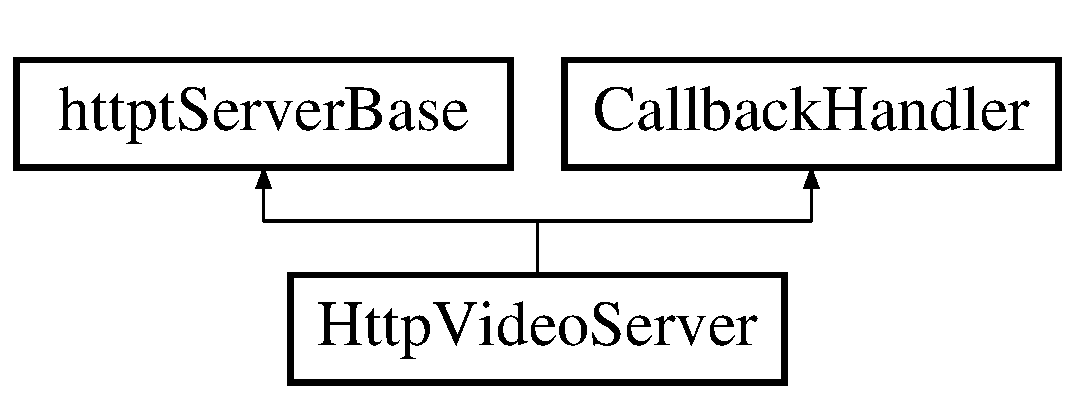
\includegraphics[height=2.000000cm]{classHttpVideoServer}
\end{center}
\end{figure}
\subsection*{Public Member Functions}
\begin{DoxyCompactItemize}
\item 
\hyperlink{classHttpVideoServer_a1d986a4456ab4b0304a8d3be52a5a8fe}{Http\+Video\+Server} ()
\item 
virtual \hyperlink{classHttpVideoServer_ab66b707c3d507d35137bfa971b3dffb7}{$\sim$\+Http\+Video\+Server} ()
\item 
double \hyperlink{classHttpVideoServer_a9a536cf80f010801085c141553e0840e}{file\+Size} ()
\item 
void \hyperlink{classHttpVideoServer_a40553e7f42d5ad39dc67a5cdaa29d396}{set\+File\+Size} (double)
\item 
double \hyperlink{classHttpVideoServer_aa2dd1fcd255474530247fa57f0732672}{piece\+Size} ()
\item 
void \hyperlink{classHttpVideoServer_a3f5282e81b55f1b70803ac535a985c16}{set\+Piece\+Size} (double)
\item 
double \hyperlink{classHttpVideoServer_a0a8769771ade7f0efb642ca9becf2eda}{block\+Size} ()
\item 
void \hyperlink{classHttpVideoServer_ab8c7c178fedee7a0fecf005bfba02038}{set\+Block\+Size} (double)
\item 
int \hyperlink{classHttpVideoServer_a83e741f6fd02aafa0147f9d9883e1709}{num\+Pieces} ()
\item 
void \hyperlink{classHttpVideoServer_ad45d130635cb7264a65461777c50bdfa}{set\+Num\+Pieces} (int)
\item 
int \hyperlink{classHttpVideoServer_afa57d2d7c4cfb9b095afab2722f74e32}{num\+Blocks} ()
\item 
void \hyperlink{classHttpVideoServer_ac6efcd99e2103e6765ce72eb4ead70c6}{set\+Num\+Blocks} (int)
\item 
\hyperlink{classBitField}{Bit\+Field} $\ast$ \hyperlink{classHttpVideoServer_a812a89eb04d1244bd38c02153741ae4b}{local\+Bitfield} ()
\item 
void \hyperlink{classHttpVideoServer_a32874ad8aee9502fee85f39e4fc85416}{initialize\+Local\+Bitfield} (bool)
\end{DoxyCompactItemize}
\subsection*{Protected Member Functions}
\begin{DoxyCompactItemize}
\item 
virtual void \hyperlink{classHttpVideoServer_a3127ef997a71295b1f6de5550958471c}{initialize} ()
\item 
virtual void \hyperlink{classHttpVideoServer_ada12e18a6a9441c9d6e6ed4d342ef152}{handle\+Message} (c\+Message $\ast$msg)
\item 
virtual void \hyperlink{classHttpVideoServer_a2dc6f992b9415e07df68d88671b644c3}{accept\+Callback} (int socket\+\_\+id, int ret\+\_\+status, void $\ast$my\+Ptr)
\item 
virtual void \hyperlink{classHttpVideoServer_aded1f1456e066d10b8d973d9c40e211c}{recv\+Callback} (int socket\+\_\+id, int ret\+\_\+status, c\+Packet $\ast$msg, void $\ast$my\+Ptr)
\end{DoxyCompactItemize}
\begin{Indent}{\bf httpt\+Server\+Base redefinitions}\par
\begin{DoxyCompactItemize}
\item 
virtual httpt\+Reply\+Message $\ast$ \hyperlink{classHttpVideoServer_acfd022e0c52ecbf11ce85dad3e7cd970}{handle\+Get\+Request} (httpt\+Request\+Message $\ast$request, string resource)
\item 
virtual void \hyperlink{classHttpVideoServer_aa127b68d76ece8f70f78350c93f62516}{update\+Display} ()
\end{DoxyCompactItemize}
\end{Indent}
\subsection*{Protected Attributes}
\begin{DoxyCompactItemize}
\item 
double \hyperlink{classHttpVideoServer_af45336d8522d6f0a882c04ea4cc4301e}{file\+\_\+size\+\_\+var}
\item 
double \hyperlink{classHttpVideoServer_a6cb1c220cced89e22cb6b945013adecb}{piece\+\_\+size\+\_\+var}
\item 
double \hyperlink{classHttpVideoServer_adf1a02001ad6ab37a3f0728df6bcb618}{block\+\_\+size\+\_\+var}
\item 
int \hyperlink{classHttpVideoServer_ae630ec3629f6a4e00a7a28e583395ee2}{num\+Pieces\+\_\+var}
\item 
int \hyperlink{classHttpVideoServer_a39d06af889c6ae735c472bd5a04d5fc5}{num\+Blocks\+\_\+var}
\item 
\hyperlink{classBitField}{Bit\+Field} $\ast$ \hyperlink{classHttpVideoServer_a8686906ce2ad0b0226567bcb0386e4f8}{local\+Bitfield\+\_\+var}
\item 
T\+C\+P\+Socket\+A\+P\+I\+\_\+\+Inet $\ast$ \hyperlink{classHttpVideoServer_ab30327bad9fa9a59dad39b759f9e83c0}{tcp\+\_\+api}
\end{DoxyCompactItemize}


\subsection{Constructor \& Destructor Documentation}
\hypertarget{classHttpVideoServer_a1d986a4456ab4b0304a8d3be52a5a8fe}{}\index{Http\+Video\+Server@{Http\+Video\+Server}!Http\+Video\+Server@{Http\+Video\+Server}}
\index{Http\+Video\+Server@{Http\+Video\+Server}!Http\+Video\+Server@{Http\+Video\+Server}}
\subsubsection[{Http\+Video\+Server()}]{\setlength{\rightskip}{0pt plus 5cm}Http\+Video\+Server\+::\+Http\+Video\+Server (
\begin{DoxyParamCaption}
{}
\end{DoxyParamCaption}
)}\label{classHttpVideoServer_a1d986a4456ab4b0304a8d3be52a5a8fe}
\hypertarget{classHttpVideoServer_ab66b707c3d507d35137bfa971b3dffb7}{}\index{Http\+Video\+Server@{Http\+Video\+Server}!````~Http\+Video\+Server@{$\sim$\+Http\+Video\+Server}}
\index{````~Http\+Video\+Server@{$\sim$\+Http\+Video\+Server}!Http\+Video\+Server@{Http\+Video\+Server}}
\subsubsection[{$\sim$\+Http\+Video\+Server()}]{\setlength{\rightskip}{0pt plus 5cm}Http\+Video\+Server\+::$\sim$\+Http\+Video\+Server (
\begin{DoxyParamCaption}
{}
\end{DoxyParamCaption}
)\hspace{0.3cm}{\ttfamily [virtual]}}\label{classHttpVideoServer_ab66b707c3d507d35137bfa971b3dffb7}


\subsection{Member Function Documentation}
\hypertarget{classHttpVideoServer_a2dc6f992b9415e07df68d88671b644c3}{}\index{Http\+Video\+Server@{Http\+Video\+Server}!accept\+Callback@{accept\+Callback}}
\index{accept\+Callback@{accept\+Callback}!Http\+Video\+Server@{Http\+Video\+Server}}
\subsubsection[{accept\+Callback(int socket\+\_\+id, int ret\+\_\+status, void $\ast$my\+Ptr)}]{\setlength{\rightskip}{0pt plus 5cm}void Http\+Video\+Server\+::accept\+Callback (
\begin{DoxyParamCaption}
\item[{int}]{socket\+\_\+id, }
\item[{int}]{ret\+\_\+status, }
\item[{void $\ast$}]{my\+Ptr}
\end{DoxyParamCaption}
)\hspace{0.3cm}{\ttfamily [protected]}, {\ttfamily [virtual]}}\label{classHttpVideoServer_a2dc6f992b9415e07df68d88671b644c3}
\hypertarget{classHttpVideoServer_a0a8769771ade7f0efb642ca9becf2eda}{}\index{Http\+Video\+Server@{Http\+Video\+Server}!block\+Size@{block\+Size}}
\index{block\+Size@{block\+Size}!Http\+Video\+Server@{Http\+Video\+Server}}
\subsubsection[{block\+Size()}]{\setlength{\rightskip}{0pt plus 5cm}double Http\+Video\+Server\+::block\+Size (
\begin{DoxyParamCaption}
{}
\end{DoxyParamCaption}
)}\label{classHttpVideoServer_a0a8769771ade7f0efb642ca9becf2eda}
\hypertarget{classHttpVideoServer_a9a536cf80f010801085c141553e0840e}{}\index{Http\+Video\+Server@{Http\+Video\+Server}!file\+Size@{file\+Size}}
\index{file\+Size@{file\+Size}!Http\+Video\+Server@{Http\+Video\+Server}}
\subsubsection[{file\+Size()}]{\setlength{\rightskip}{0pt plus 5cm}double Http\+Video\+Server\+::file\+Size (
\begin{DoxyParamCaption}
{}
\end{DoxyParamCaption}
)}\label{classHttpVideoServer_a9a536cf80f010801085c141553e0840e}
\hypertarget{classHttpVideoServer_acfd022e0c52ecbf11ce85dad3e7cd970}{}\index{Http\+Video\+Server@{Http\+Video\+Server}!handle\+Get\+Request@{handle\+Get\+Request}}
\index{handle\+Get\+Request@{handle\+Get\+Request}!Http\+Video\+Server@{Http\+Video\+Server}}
\subsubsection[{handle\+Get\+Request(httpt\+Request\+Message $\ast$request, string resource)}]{\setlength{\rightskip}{0pt plus 5cm}httpt\+Reply\+Message $\ast$ Http\+Video\+Server\+::handle\+Get\+Request (
\begin{DoxyParamCaption}
\item[{httpt\+Request\+Message $\ast$}]{request, }
\item[{string}]{resource}
\end{DoxyParamCaption}
)\hspace{0.3cm}{\ttfamily [protected]}, {\ttfamily [virtual]}}\label{classHttpVideoServer_acfd022e0c52ecbf11ce85dad3e7cd970}
\hypertarget{classHttpVideoServer_ada12e18a6a9441c9d6e6ed4d342ef152}{}\index{Http\+Video\+Server@{Http\+Video\+Server}!handle\+Message@{handle\+Message}}
\index{handle\+Message@{handle\+Message}!Http\+Video\+Server@{Http\+Video\+Server}}
\subsubsection[{handle\+Message(c\+Message $\ast$msg)}]{\setlength{\rightskip}{0pt plus 5cm}void Http\+Video\+Server\+::handle\+Message (
\begin{DoxyParamCaption}
\item[{c\+Message $\ast$}]{msg}
\end{DoxyParamCaption}
)\hspace{0.3cm}{\ttfamily [protected]}, {\ttfamily [virtual]}}\label{classHttpVideoServer_ada12e18a6a9441c9d6e6ed4d342ef152}
\hypertarget{classHttpVideoServer_a3127ef997a71295b1f6de5550958471c}{}\index{Http\+Video\+Server@{Http\+Video\+Server}!initialize@{initialize}}
\index{initialize@{initialize}!Http\+Video\+Server@{Http\+Video\+Server}}
\subsubsection[{initialize()}]{\setlength{\rightskip}{0pt plus 5cm}void Http\+Video\+Server\+::initialize (
\begin{DoxyParamCaption}
{}
\end{DoxyParamCaption}
)\hspace{0.3cm}{\ttfamily [protected]}, {\ttfamily [virtual]}}\label{classHttpVideoServer_a3127ef997a71295b1f6de5550958471c}
\hypertarget{classHttpVideoServer_a32874ad8aee9502fee85f39e4fc85416}{}\index{Http\+Video\+Server@{Http\+Video\+Server}!initialize\+Local\+Bitfield@{initialize\+Local\+Bitfield}}
\index{initialize\+Local\+Bitfield@{initialize\+Local\+Bitfield}!Http\+Video\+Server@{Http\+Video\+Server}}
\subsubsection[{initialize\+Local\+Bitfield(bool)}]{\setlength{\rightskip}{0pt plus 5cm}void Http\+Video\+Server\+::initialize\+Local\+Bitfield (
\begin{DoxyParamCaption}
\item[{bool}]{seeder}
\end{DoxyParamCaption}
)}\label{classHttpVideoServer_a32874ad8aee9502fee85f39e4fc85416}
\hypertarget{classHttpVideoServer_a812a89eb04d1244bd38c02153741ae4b}{}\index{Http\+Video\+Server@{Http\+Video\+Server}!local\+Bitfield@{local\+Bitfield}}
\index{local\+Bitfield@{local\+Bitfield}!Http\+Video\+Server@{Http\+Video\+Server}}
\subsubsection[{local\+Bitfield()}]{\setlength{\rightskip}{0pt plus 5cm}{\bf Bit\+Field} $\ast$ Http\+Video\+Server\+::local\+Bitfield (
\begin{DoxyParamCaption}
{}
\end{DoxyParamCaption}
)}\label{classHttpVideoServer_a812a89eb04d1244bd38c02153741ae4b}
\hypertarget{classHttpVideoServer_afa57d2d7c4cfb9b095afab2722f74e32}{}\index{Http\+Video\+Server@{Http\+Video\+Server}!num\+Blocks@{num\+Blocks}}
\index{num\+Blocks@{num\+Blocks}!Http\+Video\+Server@{Http\+Video\+Server}}
\subsubsection[{num\+Blocks()}]{\setlength{\rightskip}{0pt plus 5cm}int Http\+Video\+Server\+::num\+Blocks (
\begin{DoxyParamCaption}
{}
\end{DoxyParamCaption}
)}\label{classHttpVideoServer_afa57d2d7c4cfb9b095afab2722f74e32}
\hypertarget{classHttpVideoServer_a83e741f6fd02aafa0147f9d9883e1709}{}\index{Http\+Video\+Server@{Http\+Video\+Server}!num\+Pieces@{num\+Pieces}}
\index{num\+Pieces@{num\+Pieces}!Http\+Video\+Server@{Http\+Video\+Server}}
\subsubsection[{num\+Pieces()}]{\setlength{\rightskip}{0pt plus 5cm}int Http\+Video\+Server\+::num\+Pieces (
\begin{DoxyParamCaption}
{}
\end{DoxyParamCaption}
)}\label{classHttpVideoServer_a83e741f6fd02aafa0147f9d9883e1709}
\hypertarget{classHttpVideoServer_aa2dd1fcd255474530247fa57f0732672}{}\index{Http\+Video\+Server@{Http\+Video\+Server}!piece\+Size@{piece\+Size}}
\index{piece\+Size@{piece\+Size}!Http\+Video\+Server@{Http\+Video\+Server}}
\subsubsection[{piece\+Size()}]{\setlength{\rightskip}{0pt plus 5cm}double Http\+Video\+Server\+::piece\+Size (
\begin{DoxyParamCaption}
{}
\end{DoxyParamCaption}
)}\label{classHttpVideoServer_aa2dd1fcd255474530247fa57f0732672}
\hypertarget{classHttpVideoServer_aded1f1456e066d10b8d973d9c40e211c}{}\index{Http\+Video\+Server@{Http\+Video\+Server}!recv\+Callback@{recv\+Callback}}
\index{recv\+Callback@{recv\+Callback}!Http\+Video\+Server@{Http\+Video\+Server}}
\subsubsection[{recv\+Callback(int socket\+\_\+id, int ret\+\_\+status, c\+Packet $\ast$msg, void $\ast$my\+Ptr)}]{\setlength{\rightskip}{0pt plus 5cm}void Http\+Video\+Server\+::recv\+Callback (
\begin{DoxyParamCaption}
\item[{int}]{socket\+\_\+id, }
\item[{int}]{ret\+\_\+status, }
\item[{c\+Packet $\ast$}]{msg, }
\item[{void $\ast$}]{my\+Ptr}
\end{DoxyParamCaption}
)\hspace{0.3cm}{\ttfamily [protected]}, {\ttfamily [virtual]}}\label{classHttpVideoServer_aded1f1456e066d10b8d973d9c40e211c}
\hypertarget{classHttpVideoServer_ab8c7c178fedee7a0fecf005bfba02038}{}\index{Http\+Video\+Server@{Http\+Video\+Server}!set\+Block\+Size@{set\+Block\+Size}}
\index{set\+Block\+Size@{set\+Block\+Size}!Http\+Video\+Server@{Http\+Video\+Server}}
\subsubsection[{set\+Block\+Size(double)}]{\setlength{\rightskip}{0pt plus 5cm}void Http\+Video\+Server\+::set\+Block\+Size (
\begin{DoxyParamCaption}
\item[{double}]{block\+\_\+size}
\end{DoxyParamCaption}
)}\label{classHttpVideoServer_ab8c7c178fedee7a0fecf005bfba02038}
\hypertarget{classHttpVideoServer_a40553e7f42d5ad39dc67a5cdaa29d396}{}\index{Http\+Video\+Server@{Http\+Video\+Server}!set\+File\+Size@{set\+File\+Size}}
\index{set\+File\+Size@{set\+File\+Size}!Http\+Video\+Server@{Http\+Video\+Server}}
\subsubsection[{set\+File\+Size(double)}]{\setlength{\rightskip}{0pt plus 5cm}void Http\+Video\+Server\+::set\+File\+Size (
\begin{DoxyParamCaption}
\item[{double}]{file\+\_\+size}
\end{DoxyParamCaption}
)}\label{classHttpVideoServer_a40553e7f42d5ad39dc67a5cdaa29d396}
\hypertarget{classHttpVideoServer_ac6efcd99e2103e6765ce72eb4ead70c6}{}\index{Http\+Video\+Server@{Http\+Video\+Server}!set\+Num\+Blocks@{set\+Num\+Blocks}}
\index{set\+Num\+Blocks@{set\+Num\+Blocks}!Http\+Video\+Server@{Http\+Video\+Server}}
\subsubsection[{set\+Num\+Blocks(int)}]{\setlength{\rightskip}{0pt plus 5cm}void Http\+Video\+Server\+::set\+Num\+Blocks (
\begin{DoxyParamCaption}
\item[{int}]{num\+Blocks}
\end{DoxyParamCaption}
)}\label{classHttpVideoServer_ac6efcd99e2103e6765ce72eb4ead70c6}
\hypertarget{classHttpVideoServer_ad45d130635cb7264a65461777c50bdfa}{}\index{Http\+Video\+Server@{Http\+Video\+Server}!set\+Num\+Pieces@{set\+Num\+Pieces}}
\index{set\+Num\+Pieces@{set\+Num\+Pieces}!Http\+Video\+Server@{Http\+Video\+Server}}
\subsubsection[{set\+Num\+Pieces(int)}]{\setlength{\rightskip}{0pt plus 5cm}void Http\+Video\+Server\+::set\+Num\+Pieces (
\begin{DoxyParamCaption}
\item[{int}]{num\+Pieces}
\end{DoxyParamCaption}
)}\label{classHttpVideoServer_ad45d130635cb7264a65461777c50bdfa}
\hypertarget{classHttpVideoServer_a3f5282e81b55f1b70803ac535a985c16}{}\index{Http\+Video\+Server@{Http\+Video\+Server}!set\+Piece\+Size@{set\+Piece\+Size}}
\index{set\+Piece\+Size@{set\+Piece\+Size}!Http\+Video\+Server@{Http\+Video\+Server}}
\subsubsection[{set\+Piece\+Size(double)}]{\setlength{\rightskip}{0pt plus 5cm}void Http\+Video\+Server\+::set\+Piece\+Size (
\begin{DoxyParamCaption}
\item[{double}]{piece\+\_\+size}
\end{DoxyParamCaption}
)}\label{classHttpVideoServer_a3f5282e81b55f1b70803ac535a985c16}
\hypertarget{classHttpVideoServer_aa127b68d76ece8f70f78350c93f62516}{}\index{Http\+Video\+Server@{Http\+Video\+Server}!update\+Display@{update\+Display}}
\index{update\+Display@{update\+Display}!Http\+Video\+Server@{Http\+Video\+Server}}
\subsubsection[{update\+Display()}]{\setlength{\rightskip}{0pt plus 5cm}void Http\+Video\+Server\+::update\+Display (
\begin{DoxyParamCaption}
{}
\end{DoxyParamCaption}
)\hspace{0.3cm}{\ttfamily [protected]}, {\ttfamily [virtual]}}\label{classHttpVideoServer_aa127b68d76ece8f70f78350c93f62516}


\subsection{Member Data Documentation}
\hypertarget{classHttpVideoServer_adf1a02001ad6ab37a3f0728df6bcb618}{}\index{Http\+Video\+Server@{Http\+Video\+Server}!block\+\_\+size\+\_\+var@{block\+\_\+size\+\_\+var}}
\index{block\+\_\+size\+\_\+var@{block\+\_\+size\+\_\+var}!Http\+Video\+Server@{Http\+Video\+Server}}
\subsubsection[{block\+\_\+size\+\_\+var}]{\setlength{\rightskip}{0pt plus 5cm}double Http\+Video\+Server\+::block\+\_\+size\+\_\+var\hspace{0.3cm}{\ttfamily [protected]}}\label{classHttpVideoServer_adf1a02001ad6ab37a3f0728df6bcb618}
\hypertarget{classHttpVideoServer_af45336d8522d6f0a882c04ea4cc4301e}{}\index{Http\+Video\+Server@{Http\+Video\+Server}!file\+\_\+size\+\_\+var@{file\+\_\+size\+\_\+var}}
\index{file\+\_\+size\+\_\+var@{file\+\_\+size\+\_\+var}!Http\+Video\+Server@{Http\+Video\+Server}}
\subsubsection[{file\+\_\+size\+\_\+var}]{\setlength{\rightskip}{0pt plus 5cm}double Http\+Video\+Server\+::file\+\_\+size\+\_\+var\hspace{0.3cm}{\ttfamily [protected]}}\label{classHttpVideoServer_af45336d8522d6f0a882c04ea4cc4301e}
\hypertarget{classHttpVideoServer_a8686906ce2ad0b0226567bcb0386e4f8}{}\index{Http\+Video\+Server@{Http\+Video\+Server}!local\+Bitfield\+\_\+var@{local\+Bitfield\+\_\+var}}
\index{local\+Bitfield\+\_\+var@{local\+Bitfield\+\_\+var}!Http\+Video\+Server@{Http\+Video\+Server}}
\subsubsection[{local\+Bitfield\+\_\+var}]{\setlength{\rightskip}{0pt plus 5cm}{\bf Bit\+Field}$\ast$ Http\+Video\+Server\+::local\+Bitfield\+\_\+var\hspace{0.3cm}{\ttfamily [protected]}}\label{classHttpVideoServer_a8686906ce2ad0b0226567bcb0386e4f8}
\hypertarget{classHttpVideoServer_a39d06af889c6ae735c472bd5a04d5fc5}{}\index{Http\+Video\+Server@{Http\+Video\+Server}!num\+Blocks\+\_\+var@{num\+Blocks\+\_\+var}}
\index{num\+Blocks\+\_\+var@{num\+Blocks\+\_\+var}!Http\+Video\+Server@{Http\+Video\+Server}}
\subsubsection[{num\+Blocks\+\_\+var}]{\setlength{\rightskip}{0pt plus 5cm}int Http\+Video\+Server\+::num\+Blocks\+\_\+var\hspace{0.3cm}{\ttfamily [protected]}}\label{classHttpVideoServer_a39d06af889c6ae735c472bd5a04d5fc5}
\hypertarget{classHttpVideoServer_ae630ec3629f6a4e00a7a28e583395ee2}{}\index{Http\+Video\+Server@{Http\+Video\+Server}!num\+Pieces\+\_\+var@{num\+Pieces\+\_\+var}}
\index{num\+Pieces\+\_\+var@{num\+Pieces\+\_\+var}!Http\+Video\+Server@{Http\+Video\+Server}}
\subsubsection[{num\+Pieces\+\_\+var}]{\setlength{\rightskip}{0pt plus 5cm}int Http\+Video\+Server\+::num\+Pieces\+\_\+var\hspace{0.3cm}{\ttfamily [protected]}}\label{classHttpVideoServer_ae630ec3629f6a4e00a7a28e583395ee2}
\hypertarget{classHttpVideoServer_a6cb1c220cced89e22cb6b945013adecb}{}\index{Http\+Video\+Server@{Http\+Video\+Server}!piece\+\_\+size\+\_\+var@{piece\+\_\+size\+\_\+var}}
\index{piece\+\_\+size\+\_\+var@{piece\+\_\+size\+\_\+var}!Http\+Video\+Server@{Http\+Video\+Server}}
\subsubsection[{piece\+\_\+size\+\_\+var}]{\setlength{\rightskip}{0pt plus 5cm}double Http\+Video\+Server\+::piece\+\_\+size\+\_\+var\hspace{0.3cm}{\ttfamily [protected]}}\label{classHttpVideoServer_a6cb1c220cced89e22cb6b945013adecb}
\hypertarget{classHttpVideoServer_ab30327bad9fa9a59dad39b759f9e83c0}{}\index{Http\+Video\+Server@{Http\+Video\+Server}!tcp\+\_\+api@{tcp\+\_\+api}}
\index{tcp\+\_\+api@{tcp\+\_\+api}!Http\+Video\+Server@{Http\+Video\+Server}}
\subsubsection[{tcp\+\_\+api}]{\setlength{\rightskip}{0pt plus 5cm}T\+C\+P\+Socket\+A\+P\+I\+\_\+\+Inet$\ast$ Http\+Video\+Server\+::tcp\+\_\+api\hspace{0.3cm}{\ttfamily [protected]}}\label{classHttpVideoServer_ab30327bad9fa9a59dad39b759f9e83c0}


The documentation for this class was generated from the following files\+:\begin{DoxyCompactItemize}
\item 
\hyperlink{HttpVideoServer_8h}{Http\+Video\+Server.\+h}\item 
\hyperlink{HttpVideoServer_8cc}{Http\+Video\+Server.\+cc}\end{DoxyCompactItemize}

\hypertarget{structPEER}{}\section{P\+E\+E\+R Struct Reference}
\label{structPEER}\index{P\+E\+E\+R@{P\+E\+E\+R}}


{\ttfamily \#include $<$B\+T\+Tracker\+Msg\+\_\+m.\+h$>$}

\subsection*{Public Member Functions}
\begin{DoxyCompactItemize}
\item 
\hyperlink{structPEER_ac9ea3b3627396ef053f4e111bd2a08a2}{P\+E\+E\+R} ()
\end{DoxyCompactItemize}
\subsection*{Public Attributes}
\begin{DoxyCompactItemize}
\item 
opp\+\_\+string \hyperlink{structPEER_a519f6e8305967bad664558e1af9d08b9}{peer\+Id}
\item 
unsigned int \hyperlink{structPEER_a621cd69e7a189d3b0cada8322c2a22eb}{peer\+Port}
\item 
\+::I\+Pv\+X\+Address \hyperlink{structPEER_a867725ed03754bcec1086706377116d1}{ip\+Address}
\end{DoxyCompactItemize}


\subsection{Detailed Description}
Struct generated from applications/x\+Bit\+Torrent/\+B\+T\+Tracker\+Msg.\+msg by opp\+\_\+msgc. 

\subsection{Constructor \& Destructor Documentation}
\hypertarget{structPEER_ac9ea3b3627396ef053f4e111bd2a08a2}{}\index{P\+E\+E\+R@{P\+E\+E\+R}!P\+E\+E\+R@{P\+E\+E\+R}}
\index{P\+E\+E\+R@{P\+E\+E\+R}!P\+E\+E\+R@{P\+E\+E\+R}}
\subsubsection[{P\+E\+E\+R()}]{\setlength{\rightskip}{0pt plus 5cm}P\+E\+E\+R\+::\+P\+E\+E\+R (
\begin{DoxyParamCaption}
{}
\end{DoxyParamCaption}
)}\label{structPEER_ac9ea3b3627396ef053f4e111bd2a08a2}


\subsection{Member Data Documentation}
\hypertarget{structPEER_a867725ed03754bcec1086706377116d1}{}\index{P\+E\+E\+R@{P\+E\+E\+R}!ip\+Address@{ip\+Address}}
\index{ip\+Address@{ip\+Address}!P\+E\+E\+R@{P\+E\+E\+R}}
\subsubsection[{ip\+Address}]{\setlength{\rightskip}{0pt plus 5cm}\+::I\+Pv\+X\+Address P\+E\+E\+R\+::ip\+Address}\label{structPEER_a867725ed03754bcec1086706377116d1}
\hypertarget{structPEER_a519f6e8305967bad664558e1af9d08b9}{}\index{P\+E\+E\+R@{P\+E\+E\+R}!peer\+Id@{peer\+Id}}
\index{peer\+Id@{peer\+Id}!P\+E\+E\+R@{P\+E\+E\+R}}
\subsubsection[{peer\+Id}]{\setlength{\rightskip}{0pt plus 5cm}opp\+\_\+string P\+E\+E\+R\+::peer\+Id}\label{structPEER_a519f6e8305967bad664558e1af9d08b9}
\hypertarget{structPEER_a621cd69e7a189d3b0cada8322c2a22eb}{}\index{P\+E\+E\+R@{P\+E\+E\+R}!peer\+Port@{peer\+Port}}
\index{peer\+Port@{peer\+Port}!P\+E\+E\+R@{P\+E\+E\+R}}
\subsubsection[{peer\+Port}]{\setlength{\rightskip}{0pt plus 5cm}unsigned int P\+E\+E\+R\+::peer\+Port}\label{structPEER_a621cd69e7a189d3b0cada8322c2a22eb}


The documentation for this struct was generated from the following files\+:\begin{DoxyCompactItemize}
\item 
\hyperlink{BTTrackerMsg__m_8h}{B\+T\+Tracker\+Msg\+\_\+m.\+h}\item 
\hyperlink{BTTrackerMsg__m_8cc}{B\+T\+Tracker\+Msg\+\_\+m.\+cc}\end{DoxyCompactItemize}

\hypertarget{classPEERDescriptor}{}\section{P\+E\+E\+R\+Descriptor Class Reference}
\label{classPEERDescriptor}\index{P\+E\+E\+R\+Descriptor@{P\+E\+E\+R\+Descriptor}}
Inheritance diagram for P\+E\+E\+R\+Descriptor\+:\begin{figure}[H]
\begin{center}
\leavevmode
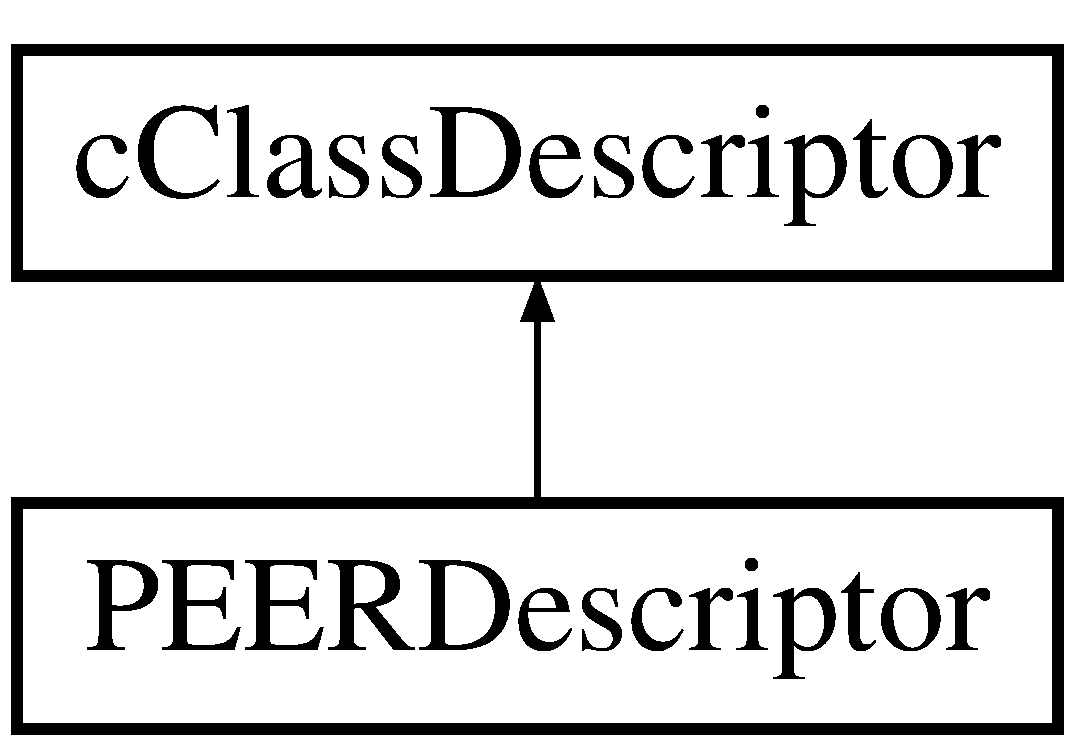
\includegraphics[height=2.000000cm]{classPEERDescriptor}
\end{center}
\end{figure}
\subsection*{Public Member Functions}
\begin{DoxyCompactItemize}
\item 
\hyperlink{classPEERDescriptor_ac98eff6a4b6c650837a30fed9c58c898}{P\+E\+E\+R\+Descriptor} ()
\item 
virtual \hyperlink{classPEERDescriptor_abf8331c8a195deb922ae54b79509885a}{$\sim$\+P\+E\+E\+R\+Descriptor} ()
\item 
virtual bool \hyperlink{classPEERDescriptor_a71f8aed4263732caea706370588b5d11}{does\+Support} (c\+Object $\ast$obj) const 
\item 
virtual const char $\ast$ \hyperlink{classPEERDescriptor_a67f9ff91d82dd253b3ff013dfa7eada1}{get\+Property} (const char $\ast$propertyname) const 
\item 
virtual int \hyperlink{classPEERDescriptor_ac805efcb83b73c29bb8f4efde0465fac}{get\+Field\+Count} (void $\ast$object) const 
\item 
virtual const char $\ast$ \hyperlink{classPEERDescriptor_a44eae399e462eb0449bf250965b827c0}{get\+Field\+Name} (void $\ast$object, int field) const 
\item 
virtual int \hyperlink{classPEERDescriptor_af0d287d7ccab253dc32a122aa39d0fcc}{find\+Field} (void $\ast$object, const char $\ast$field\+Name) const 
\item 
virtual unsigned int \hyperlink{classPEERDescriptor_a373bcb2666b13e2f6581f913789b1bf3}{get\+Field\+Type\+Flags} (void $\ast$object, int field) const 
\item 
virtual const char $\ast$ \hyperlink{classPEERDescriptor_a52237786e198ff037c1976468dcfd8e4}{get\+Field\+Type\+String} (void $\ast$object, int field) const 
\item 
virtual const char $\ast$ \hyperlink{classPEERDescriptor_a99156bb4a82bf0553767f0c895e23f3a}{get\+Field\+Property} (void $\ast$object, int field, const char $\ast$propertyname) const 
\item 
virtual int \hyperlink{classPEERDescriptor_a455e1229cc84b23d10e2261e15bce00a}{get\+Array\+Size} (void $\ast$object, int field) const 
\item 
virtual std\+::string \hyperlink{classPEERDescriptor_aeb00ffe24fa93000e3ea61a5d6f38283}{get\+Field\+As\+String} (void $\ast$object, int field, int i) const 
\item 
virtual bool \hyperlink{classPEERDescriptor_a97515c2d476c4100da4716faee598086}{set\+Field\+As\+String} (void $\ast$object, int field, int i, const char $\ast$value) const 
\item 
virtual const char $\ast$ \hyperlink{classPEERDescriptor_a79210a46adb78f48670cb1b42dbbce69}{get\+Field\+Struct\+Name} (void $\ast$object, int field) const 
\item 
virtual void $\ast$ \hyperlink{classPEERDescriptor_a41a4358d8479ca681313acd6fa82ec46}{get\+Field\+Struct\+Pointer} (void $\ast$object, int field, int i) const 
\end{DoxyCompactItemize}


\subsection{Constructor \& Destructor Documentation}
\hypertarget{classPEERDescriptor_ac98eff6a4b6c650837a30fed9c58c898}{}\index{P\+E\+E\+R\+Descriptor@{P\+E\+E\+R\+Descriptor}!P\+E\+E\+R\+Descriptor@{P\+E\+E\+R\+Descriptor}}
\index{P\+E\+E\+R\+Descriptor@{P\+E\+E\+R\+Descriptor}!P\+E\+E\+R\+Descriptor@{P\+E\+E\+R\+Descriptor}}
\subsubsection[{P\+E\+E\+R\+Descriptor()}]{\setlength{\rightskip}{0pt plus 5cm}P\+E\+E\+R\+Descriptor\+::\+P\+E\+E\+R\+Descriptor (
\begin{DoxyParamCaption}
{}
\end{DoxyParamCaption}
)}\label{classPEERDescriptor_ac98eff6a4b6c650837a30fed9c58c898}
\hypertarget{classPEERDescriptor_abf8331c8a195deb922ae54b79509885a}{}\index{P\+E\+E\+R\+Descriptor@{P\+E\+E\+R\+Descriptor}!````~P\+E\+E\+R\+Descriptor@{$\sim$\+P\+E\+E\+R\+Descriptor}}
\index{````~P\+E\+E\+R\+Descriptor@{$\sim$\+P\+E\+E\+R\+Descriptor}!P\+E\+E\+R\+Descriptor@{P\+E\+E\+R\+Descriptor}}
\subsubsection[{$\sim$\+P\+E\+E\+R\+Descriptor()}]{\setlength{\rightskip}{0pt plus 5cm}P\+E\+E\+R\+Descriptor\+::$\sim$\+P\+E\+E\+R\+Descriptor (
\begin{DoxyParamCaption}
{}
\end{DoxyParamCaption}
)\hspace{0.3cm}{\ttfamily [virtual]}}\label{classPEERDescriptor_abf8331c8a195deb922ae54b79509885a}


\subsection{Member Function Documentation}
\hypertarget{classPEERDescriptor_a71f8aed4263732caea706370588b5d11}{}\index{P\+E\+E\+R\+Descriptor@{P\+E\+E\+R\+Descriptor}!does\+Support@{does\+Support}}
\index{does\+Support@{does\+Support}!P\+E\+E\+R\+Descriptor@{P\+E\+E\+R\+Descriptor}}
\subsubsection[{does\+Support(c\+Object $\ast$obj) const }]{\setlength{\rightskip}{0pt plus 5cm}bool P\+E\+E\+R\+Descriptor\+::does\+Support (
\begin{DoxyParamCaption}
\item[{c\+Object $\ast$}]{obj}
\end{DoxyParamCaption}
) const\hspace{0.3cm}{\ttfamily [virtual]}}\label{classPEERDescriptor_a71f8aed4263732caea706370588b5d11}
\hypertarget{classPEERDescriptor_af0d287d7ccab253dc32a122aa39d0fcc}{}\index{P\+E\+E\+R\+Descriptor@{P\+E\+E\+R\+Descriptor}!find\+Field@{find\+Field}}
\index{find\+Field@{find\+Field}!P\+E\+E\+R\+Descriptor@{P\+E\+E\+R\+Descriptor}}
\subsubsection[{find\+Field(void $\ast$object, const char $\ast$field\+Name) const }]{\setlength{\rightskip}{0pt plus 5cm}int P\+E\+E\+R\+Descriptor\+::find\+Field (
\begin{DoxyParamCaption}
\item[{void $\ast$}]{object, }
\item[{const char $\ast$}]{field\+Name}
\end{DoxyParamCaption}
) const\hspace{0.3cm}{\ttfamily [virtual]}}\label{classPEERDescriptor_af0d287d7ccab253dc32a122aa39d0fcc}
\hypertarget{classPEERDescriptor_a455e1229cc84b23d10e2261e15bce00a}{}\index{P\+E\+E\+R\+Descriptor@{P\+E\+E\+R\+Descriptor}!get\+Array\+Size@{get\+Array\+Size}}
\index{get\+Array\+Size@{get\+Array\+Size}!P\+E\+E\+R\+Descriptor@{P\+E\+E\+R\+Descriptor}}
\subsubsection[{get\+Array\+Size(void $\ast$object, int field) const }]{\setlength{\rightskip}{0pt plus 5cm}int P\+E\+E\+R\+Descriptor\+::get\+Array\+Size (
\begin{DoxyParamCaption}
\item[{void $\ast$}]{object, }
\item[{int}]{field}
\end{DoxyParamCaption}
) const\hspace{0.3cm}{\ttfamily [virtual]}}\label{classPEERDescriptor_a455e1229cc84b23d10e2261e15bce00a}
\hypertarget{classPEERDescriptor_aeb00ffe24fa93000e3ea61a5d6f38283}{}\index{P\+E\+E\+R\+Descriptor@{P\+E\+E\+R\+Descriptor}!get\+Field\+As\+String@{get\+Field\+As\+String}}
\index{get\+Field\+As\+String@{get\+Field\+As\+String}!P\+E\+E\+R\+Descriptor@{P\+E\+E\+R\+Descriptor}}
\subsubsection[{get\+Field\+As\+String(void $\ast$object, int field, int i) const }]{\setlength{\rightskip}{0pt plus 5cm}std\+::string P\+E\+E\+R\+Descriptor\+::get\+Field\+As\+String (
\begin{DoxyParamCaption}
\item[{void $\ast$}]{object, }
\item[{int}]{field, }
\item[{int}]{i}
\end{DoxyParamCaption}
) const\hspace{0.3cm}{\ttfamily [virtual]}}\label{classPEERDescriptor_aeb00ffe24fa93000e3ea61a5d6f38283}
\hypertarget{classPEERDescriptor_ac805efcb83b73c29bb8f4efde0465fac}{}\index{P\+E\+E\+R\+Descriptor@{P\+E\+E\+R\+Descriptor}!get\+Field\+Count@{get\+Field\+Count}}
\index{get\+Field\+Count@{get\+Field\+Count}!P\+E\+E\+R\+Descriptor@{P\+E\+E\+R\+Descriptor}}
\subsubsection[{get\+Field\+Count(void $\ast$object) const }]{\setlength{\rightskip}{0pt plus 5cm}int P\+E\+E\+R\+Descriptor\+::get\+Field\+Count (
\begin{DoxyParamCaption}
\item[{void $\ast$}]{object}
\end{DoxyParamCaption}
) const\hspace{0.3cm}{\ttfamily [virtual]}}\label{classPEERDescriptor_ac805efcb83b73c29bb8f4efde0465fac}
\hypertarget{classPEERDescriptor_a44eae399e462eb0449bf250965b827c0}{}\index{P\+E\+E\+R\+Descriptor@{P\+E\+E\+R\+Descriptor}!get\+Field\+Name@{get\+Field\+Name}}
\index{get\+Field\+Name@{get\+Field\+Name}!P\+E\+E\+R\+Descriptor@{P\+E\+E\+R\+Descriptor}}
\subsubsection[{get\+Field\+Name(void $\ast$object, int field) const }]{\setlength{\rightskip}{0pt plus 5cm}const char $\ast$ P\+E\+E\+R\+Descriptor\+::get\+Field\+Name (
\begin{DoxyParamCaption}
\item[{void $\ast$}]{object, }
\item[{int}]{field}
\end{DoxyParamCaption}
) const\hspace{0.3cm}{\ttfamily [virtual]}}\label{classPEERDescriptor_a44eae399e462eb0449bf250965b827c0}
\hypertarget{classPEERDescriptor_a99156bb4a82bf0553767f0c895e23f3a}{}\index{P\+E\+E\+R\+Descriptor@{P\+E\+E\+R\+Descriptor}!get\+Field\+Property@{get\+Field\+Property}}
\index{get\+Field\+Property@{get\+Field\+Property}!P\+E\+E\+R\+Descriptor@{P\+E\+E\+R\+Descriptor}}
\subsubsection[{get\+Field\+Property(void $\ast$object, int field, const char $\ast$propertyname) const }]{\setlength{\rightskip}{0pt plus 5cm}const char $\ast$ P\+E\+E\+R\+Descriptor\+::get\+Field\+Property (
\begin{DoxyParamCaption}
\item[{void $\ast$}]{object, }
\item[{int}]{field, }
\item[{const char $\ast$}]{propertyname}
\end{DoxyParamCaption}
) const\hspace{0.3cm}{\ttfamily [virtual]}}\label{classPEERDescriptor_a99156bb4a82bf0553767f0c895e23f3a}
\hypertarget{classPEERDescriptor_a79210a46adb78f48670cb1b42dbbce69}{}\index{P\+E\+E\+R\+Descriptor@{P\+E\+E\+R\+Descriptor}!get\+Field\+Struct\+Name@{get\+Field\+Struct\+Name}}
\index{get\+Field\+Struct\+Name@{get\+Field\+Struct\+Name}!P\+E\+E\+R\+Descriptor@{P\+E\+E\+R\+Descriptor}}
\subsubsection[{get\+Field\+Struct\+Name(void $\ast$object, int field) const }]{\setlength{\rightskip}{0pt plus 5cm}const char $\ast$ P\+E\+E\+R\+Descriptor\+::get\+Field\+Struct\+Name (
\begin{DoxyParamCaption}
\item[{void $\ast$}]{object, }
\item[{int}]{field}
\end{DoxyParamCaption}
) const\hspace{0.3cm}{\ttfamily [virtual]}}\label{classPEERDescriptor_a79210a46adb78f48670cb1b42dbbce69}
\hypertarget{classPEERDescriptor_a41a4358d8479ca681313acd6fa82ec46}{}\index{P\+E\+E\+R\+Descriptor@{P\+E\+E\+R\+Descriptor}!get\+Field\+Struct\+Pointer@{get\+Field\+Struct\+Pointer}}
\index{get\+Field\+Struct\+Pointer@{get\+Field\+Struct\+Pointer}!P\+E\+E\+R\+Descriptor@{P\+E\+E\+R\+Descriptor}}
\subsubsection[{get\+Field\+Struct\+Pointer(void $\ast$object, int field, int i) const }]{\setlength{\rightskip}{0pt plus 5cm}void $\ast$ P\+E\+E\+R\+Descriptor\+::get\+Field\+Struct\+Pointer (
\begin{DoxyParamCaption}
\item[{void $\ast$}]{object, }
\item[{int}]{field, }
\item[{int}]{i}
\end{DoxyParamCaption}
) const\hspace{0.3cm}{\ttfamily [virtual]}}\label{classPEERDescriptor_a41a4358d8479ca681313acd6fa82ec46}
\hypertarget{classPEERDescriptor_a373bcb2666b13e2f6581f913789b1bf3}{}\index{P\+E\+E\+R\+Descriptor@{P\+E\+E\+R\+Descriptor}!get\+Field\+Type\+Flags@{get\+Field\+Type\+Flags}}
\index{get\+Field\+Type\+Flags@{get\+Field\+Type\+Flags}!P\+E\+E\+R\+Descriptor@{P\+E\+E\+R\+Descriptor}}
\subsubsection[{get\+Field\+Type\+Flags(void $\ast$object, int field) const }]{\setlength{\rightskip}{0pt plus 5cm}unsigned int P\+E\+E\+R\+Descriptor\+::get\+Field\+Type\+Flags (
\begin{DoxyParamCaption}
\item[{void $\ast$}]{object, }
\item[{int}]{field}
\end{DoxyParamCaption}
) const\hspace{0.3cm}{\ttfamily [virtual]}}\label{classPEERDescriptor_a373bcb2666b13e2f6581f913789b1bf3}
\hypertarget{classPEERDescriptor_a52237786e198ff037c1976468dcfd8e4}{}\index{P\+E\+E\+R\+Descriptor@{P\+E\+E\+R\+Descriptor}!get\+Field\+Type\+String@{get\+Field\+Type\+String}}
\index{get\+Field\+Type\+String@{get\+Field\+Type\+String}!P\+E\+E\+R\+Descriptor@{P\+E\+E\+R\+Descriptor}}
\subsubsection[{get\+Field\+Type\+String(void $\ast$object, int field) const }]{\setlength{\rightskip}{0pt plus 5cm}const char $\ast$ P\+E\+E\+R\+Descriptor\+::get\+Field\+Type\+String (
\begin{DoxyParamCaption}
\item[{void $\ast$}]{object, }
\item[{int}]{field}
\end{DoxyParamCaption}
) const\hspace{0.3cm}{\ttfamily [virtual]}}\label{classPEERDescriptor_a52237786e198ff037c1976468dcfd8e4}
\hypertarget{classPEERDescriptor_a67f9ff91d82dd253b3ff013dfa7eada1}{}\index{P\+E\+E\+R\+Descriptor@{P\+E\+E\+R\+Descriptor}!get\+Property@{get\+Property}}
\index{get\+Property@{get\+Property}!P\+E\+E\+R\+Descriptor@{P\+E\+E\+R\+Descriptor}}
\subsubsection[{get\+Property(const char $\ast$propertyname) const }]{\setlength{\rightskip}{0pt plus 5cm}const char $\ast$ P\+E\+E\+R\+Descriptor\+::get\+Property (
\begin{DoxyParamCaption}
\item[{const char $\ast$}]{propertyname}
\end{DoxyParamCaption}
) const\hspace{0.3cm}{\ttfamily [virtual]}}\label{classPEERDescriptor_a67f9ff91d82dd253b3ff013dfa7eada1}
\hypertarget{classPEERDescriptor_a97515c2d476c4100da4716faee598086}{}\index{P\+E\+E\+R\+Descriptor@{P\+E\+E\+R\+Descriptor}!set\+Field\+As\+String@{set\+Field\+As\+String}}
\index{set\+Field\+As\+String@{set\+Field\+As\+String}!P\+E\+E\+R\+Descriptor@{P\+E\+E\+R\+Descriptor}}
\subsubsection[{set\+Field\+As\+String(void $\ast$object, int field, int i, const char $\ast$value) const }]{\setlength{\rightskip}{0pt plus 5cm}bool P\+E\+E\+R\+Descriptor\+::set\+Field\+As\+String (
\begin{DoxyParamCaption}
\item[{void $\ast$}]{object, }
\item[{int}]{field, }
\item[{int}]{i, }
\item[{const char $\ast$}]{value}
\end{DoxyParamCaption}
) const\hspace{0.3cm}{\ttfamily [virtual]}}\label{classPEERDescriptor_a97515c2d476c4100da4716faee598086}


The documentation for this class was generated from the following file\+:\begin{DoxyCompactItemize}
\item 
\hyperlink{BTTrackerMsg__m_8cc}{B\+T\+Tracker\+Msg\+\_\+m.\+cc}\end{DoxyCompactItemize}

\hypertarget{classPeerEntry}{}\section{Peer\+Entry Class Reference}
\label{classPeerEntry}\index{Peer\+Entry@{Peer\+Entry}}


{\ttfamily \#include $<$B\+T\+Utils.\+h$>$}

Inheritance diagram for Peer\+Entry\+:\begin{figure}[H]
\begin{center}
\leavevmode
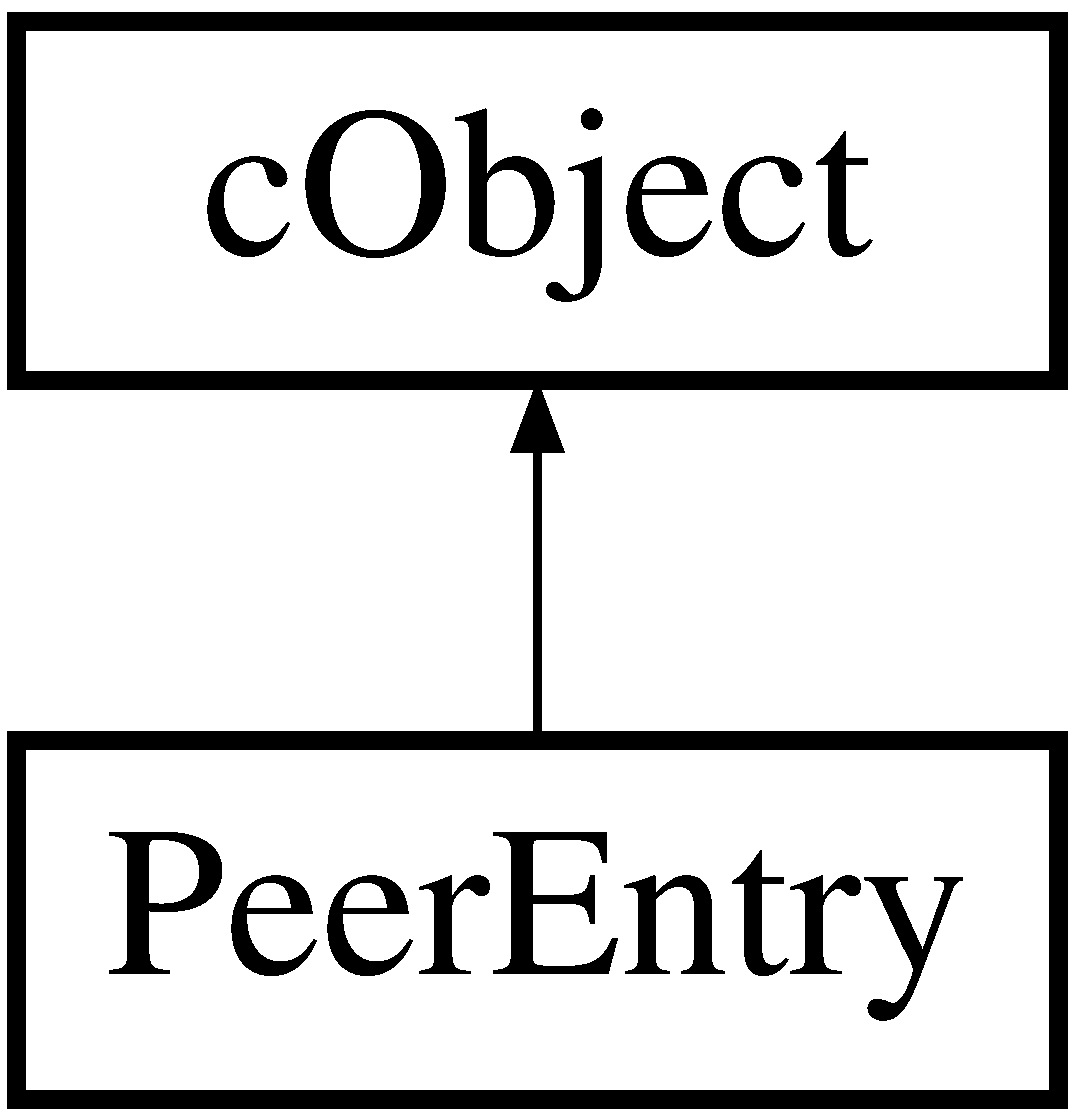
\includegraphics[height=2.000000cm]{classPeerEntry}
\end{center}
\end{figure}
\subsection*{Public Member Functions}
\begin{DoxyCompactItemize}
\item 
\hyperlink{classPeerEntry_a4ee1f78b5c23cd7762cd399b5a5e8e58}{Peer\+Entry} ()
\item 
\hyperlink{classPeerEntry_a8a4776f60687e12738d39b99878a34b6}{Peer\+Entry} (\hyperlink{structPEER}{P\+E\+E\+R}, T\+C\+P\+Server\+Thread\+Base $\ast$, double)
\item 
\hyperlink{classPeerEntry_a6ac51e17ae2ca055ac80cffa93e9d074}{Peer\+Entry} (const \hyperlink{classPeerEntry}{Peer\+Entry} \&)
\item 
virtual \hyperlink{classPeerEntry_a4910d2784aea7a78d6a595e6d533af36}{$\sim$\+Peer\+Entry} ()
\item 
string \hyperlink{classPeerEntry_ad9d39bcf7ef8e4544b3a0ceee9e5b94f}{get\+Peer\+I\+D} ()
\item 
I\+Pv\+X\+Address \hyperlink{classPeerEntry_a387e85f61fe883e5020d415c35a0f79d}{get\+Peer\+I\+P} ()
\item 
unsigned int \hyperlink{classPeerEntry_a78b6e66766700afbf24b30abeacd7583}{get\+Peer\+Port} ()
\item 
void \hyperlink{classPeerEntry_a65594d3c04eded4743909e160db3e923}{set\+Peer\+I\+D} (opp\+\_\+string)
\item 
\hyperlink{structPEER}{P\+E\+E\+R} \hyperlink{classPeerEntry_a145089116f45cc2c8a06b7989a927c89}{get\+Peer} ()
\item 
void \hyperlink{classPeerEntry_a8a7932c0dcfdedf7b758d0794eea9015}{set\+Peer} (\hyperlink{structPEER}{P\+E\+E\+R} peer)
\item 
T\+C\+P\+Server\+Thread\+Base $\ast$ \hyperlink{classPeerEntry_a29fdb30de6469f154ae1fdb97bff9704}{get\+Peer\+Thread} ()
\item 
bool \hyperlink{classPeerEntry_ac1e496d1d68c52527fb192158dddc045}{operator$<$} (const \hyperlink{classPeerEntry}{Peer\+Entry} \&) const 
\item 
bool \hyperlink{classPeerEntry_ad71e7231029292b90b8100fc0604fb25}{is\+Valid} ()
\item 
double \hyperlink{classPeerEntry_a4c0f40b9bac8e4327b46f1b7f2c9d955}{conn\+Time} ()
\item 
void \hyperlink{classPeerEntry_a342f838cb5c7f4a1865a1cb6962c24fa}{set\+Conn\+Time} (double)
\end{DoxyCompactItemize}
\subsection*{Protected Attributes}
\begin{DoxyCompactItemize}
\item 
\hyperlink{structPEER}{P\+E\+E\+R} \hyperlink{classPeerEntry_a65fcdc0c83cb8f3e2b59ef19c067504f}{peer\+Info}
\item 
T\+C\+P\+Server\+Thread\+Base $\ast$ \hyperlink{classPeerEntry_a75511a2a33f122eb90d7108164f040c9}{thread}
\item 
double \hyperlink{classPeerEntry_aa44bee1c1c87de58c0b64dcdce6273d7}{conn\+Time\+\_\+var}
\end{DoxyCompactItemize}


\subsection{Constructor \& Destructor Documentation}
\hypertarget{classPeerEntry_a4ee1f78b5c23cd7762cd399b5a5e8e58}{}\index{Peer\+Entry@{Peer\+Entry}!Peer\+Entry@{Peer\+Entry}}
\index{Peer\+Entry@{Peer\+Entry}!Peer\+Entry@{Peer\+Entry}}
\subsubsection[{Peer\+Entry()}]{\setlength{\rightskip}{0pt plus 5cm}Peer\+Entry\+::\+Peer\+Entry (
\begin{DoxyParamCaption}
{}
\end{DoxyParamCaption}
)}\label{classPeerEntry_a4ee1f78b5c23cd7762cd399b5a5e8e58}
\hypertarget{classPeerEntry_a8a4776f60687e12738d39b99878a34b6}{}\index{Peer\+Entry@{Peer\+Entry}!Peer\+Entry@{Peer\+Entry}}
\index{Peer\+Entry@{Peer\+Entry}!Peer\+Entry@{Peer\+Entry}}
\subsubsection[{Peer\+Entry(\+P\+E\+E\+R, T\+C\+P\+Server\+Thread\+Base $\ast$, double)}]{\setlength{\rightskip}{0pt plus 5cm}Peer\+Entry\+::\+Peer\+Entry (
\begin{DoxyParamCaption}
\item[{{\bf P\+E\+E\+R}}]{peer, }
\item[{T\+C\+P\+Server\+Thread\+Base $\ast$}]{thread, }
\item[{double}]{conn\+Time}
\end{DoxyParamCaption}
)}\label{classPeerEntry_a8a4776f60687e12738d39b99878a34b6}
\hypertarget{classPeerEntry_a6ac51e17ae2ca055ac80cffa93e9d074}{}\index{Peer\+Entry@{Peer\+Entry}!Peer\+Entry@{Peer\+Entry}}
\index{Peer\+Entry@{Peer\+Entry}!Peer\+Entry@{Peer\+Entry}}
\subsubsection[{Peer\+Entry(const Peer\+Entry \&)}]{\setlength{\rightskip}{0pt plus 5cm}Peer\+Entry\+::\+Peer\+Entry (
\begin{DoxyParamCaption}
\item[{const {\bf Peer\+Entry} \&}]{pe}
\end{DoxyParamCaption}
)}\label{classPeerEntry_a6ac51e17ae2ca055ac80cffa93e9d074}
\hypertarget{classPeerEntry_a4910d2784aea7a78d6a595e6d533af36}{}\index{Peer\+Entry@{Peer\+Entry}!````~Peer\+Entry@{$\sim$\+Peer\+Entry}}
\index{````~Peer\+Entry@{$\sim$\+Peer\+Entry}!Peer\+Entry@{Peer\+Entry}}
\subsubsection[{$\sim$\+Peer\+Entry()}]{\setlength{\rightskip}{0pt plus 5cm}Peer\+Entry\+::$\sim$\+Peer\+Entry (
\begin{DoxyParamCaption}
{}
\end{DoxyParamCaption}
)\hspace{0.3cm}{\ttfamily [virtual]}}\label{classPeerEntry_a4910d2784aea7a78d6a595e6d533af36}


\subsection{Member Function Documentation}
\hypertarget{classPeerEntry_a4c0f40b9bac8e4327b46f1b7f2c9d955}{}\index{Peer\+Entry@{Peer\+Entry}!conn\+Time@{conn\+Time}}
\index{conn\+Time@{conn\+Time}!Peer\+Entry@{Peer\+Entry}}
\subsubsection[{conn\+Time()}]{\setlength{\rightskip}{0pt plus 5cm}double Peer\+Entry\+::conn\+Time (
\begin{DoxyParamCaption}
{}
\end{DoxyParamCaption}
)}\label{classPeerEntry_a4c0f40b9bac8e4327b46f1b7f2c9d955}
\hypertarget{classPeerEntry_a145089116f45cc2c8a06b7989a927c89}{}\index{Peer\+Entry@{Peer\+Entry}!get\+Peer@{get\+Peer}}
\index{get\+Peer@{get\+Peer}!Peer\+Entry@{Peer\+Entry}}
\subsubsection[{get\+Peer()}]{\setlength{\rightskip}{0pt plus 5cm}{\bf P\+E\+E\+R} Peer\+Entry\+::get\+Peer (
\begin{DoxyParamCaption}
{}
\end{DoxyParamCaption}
)}\label{classPeerEntry_a145089116f45cc2c8a06b7989a927c89}
\hypertarget{classPeerEntry_ad9d39bcf7ef8e4544b3a0ceee9e5b94f}{}\index{Peer\+Entry@{Peer\+Entry}!get\+Peer\+I\+D@{get\+Peer\+I\+D}}
\index{get\+Peer\+I\+D@{get\+Peer\+I\+D}!Peer\+Entry@{Peer\+Entry}}
\subsubsection[{get\+Peer\+I\+D()}]{\setlength{\rightskip}{0pt plus 5cm}string Peer\+Entry\+::get\+Peer\+I\+D (
\begin{DoxyParamCaption}
{}
\end{DoxyParamCaption}
)}\label{classPeerEntry_ad9d39bcf7ef8e4544b3a0ceee9e5b94f}
\hypertarget{classPeerEntry_a387e85f61fe883e5020d415c35a0f79d}{}\index{Peer\+Entry@{Peer\+Entry}!get\+Peer\+I\+P@{get\+Peer\+I\+P}}
\index{get\+Peer\+I\+P@{get\+Peer\+I\+P}!Peer\+Entry@{Peer\+Entry}}
\subsubsection[{get\+Peer\+I\+P()}]{\setlength{\rightskip}{0pt plus 5cm}I\+Pv\+X\+Address Peer\+Entry\+::get\+Peer\+I\+P (
\begin{DoxyParamCaption}
{}
\end{DoxyParamCaption}
)}\label{classPeerEntry_a387e85f61fe883e5020d415c35a0f79d}
\hypertarget{classPeerEntry_a78b6e66766700afbf24b30abeacd7583}{}\index{Peer\+Entry@{Peer\+Entry}!get\+Peer\+Port@{get\+Peer\+Port}}
\index{get\+Peer\+Port@{get\+Peer\+Port}!Peer\+Entry@{Peer\+Entry}}
\subsubsection[{get\+Peer\+Port()}]{\setlength{\rightskip}{0pt plus 5cm}unsigned int Peer\+Entry\+::get\+Peer\+Port (
\begin{DoxyParamCaption}
{}
\end{DoxyParamCaption}
)}\label{classPeerEntry_a78b6e66766700afbf24b30abeacd7583}
\hypertarget{classPeerEntry_a29fdb30de6469f154ae1fdb97bff9704}{}\index{Peer\+Entry@{Peer\+Entry}!get\+Peer\+Thread@{get\+Peer\+Thread}}
\index{get\+Peer\+Thread@{get\+Peer\+Thread}!Peer\+Entry@{Peer\+Entry}}
\subsubsection[{get\+Peer\+Thread()}]{\setlength{\rightskip}{0pt plus 5cm}T\+C\+P\+Server\+Thread\+Base $\ast$ Peer\+Entry\+::get\+Peer\+Thread (
\begin{DoxyParamCaption}
{}
\end{DoxyParamCaption}
)}\label{classPeerEntry_a29fdb30de6469f154ae1fdb97bff9704}
\hypertarget{classPeerEntry_ad71e7231029292b90b8100fc0604fb25}{}\index{Peer\+Entry@{Peer\+Entry}!is\+Valid@{is\+Valid}}
\index{is\+Valid@{is\+Valid}!Peer\+Entry@{Peer\+Entry}}
\subsubsection[{is\+Valid()}]{\setlength{\rightskip}{0pt plus 5cm}bool Peer\+Entry\+::is\+Valid (
\begin{DoxyParamCaption}
{}
\end{DoxyParamCaption}
)}\label{classPeerEntry_ad71e7231029292b90b8100fc0604fb25}
\hypertarget{classPeerEntry_ac1e496d1d68c52527fb192158dddc045}{}\index{Peer\+Entry@{Peer\+Entry}!operator$<$@{operator$<$}}
\index{operator$<$@{operator$<$}!Peer\+Entry@{Peer\+Entry}}
\subsubsection[{operator$<$(const Peer\+Entry \&) const }]{\setlength{\rightskip}{0pt plus 5cm}bool Peer\+Entry\+::operator$<$ (
\begin{DoxyParamCaption}
\item[{const {\bf Peer\+Entry} \&}]{item}
\end{DoxyParamCaption}
) const}\label{classPeerEntry_ac1e496d1d68c52527fb192158dddc045}
\hypertarget{classPeerEntry_a342f838cb5c7f4a1865a1cb6962c24fa}{}\index{Peer\+Entry@{Peer\+Entry}!set\+Conn\+Time@{set\+Conn\+Time}}
\index{set\+Conn\+Time@{set\+Conn\+Time}!Peer\+Entry@{Peer\+Entry}}
\subsubsection[{set\+Conn\+Time(double)}]{\setlength{\rightskip}{0pt plus 5cm}void Peer\+Entry\+::set\+Conn\+Time (
\begin{DoxyParamCaption}
\item[{double}]{conn\+Time}
\end{DoxyParamCaption}
)}\label{classPeerEntry_a342f838cb5c7f4a1865a1cb6962c24fa}
\hypertarget{classPeerEntry_a8a7932c0dcfdedf7b758d0794eea9015}{}\index{Peer\+Entry@{Peer\+Entry}!set\+Peer@{set\+Peer}}
\index{set\+Peer@{set\+Peer}!Peer\+Entry@{Peer\+Entry}}
\subsubsection[{set\+Peer(\+P\+E\+E\+R peer)}]{\setlength{\rightskip}{0pt plus 5cm}void Peer\+Entry\+::set\+Peer (
\begin{DoxyParamCaption}
\item[{{\bf P\+E\+E\+R}}]{peer}
\end{DoxyParamCaption}
)}\label{classPeerEntry_a8a7932c0dcfdedf7b758d0794eea9015}
\hypertarget{classPeerEntry_a65594d3c04eded4743909e160db3e923}{}\index{Peer\+Entry@{Peer\+Entry}!set\+Peer\+I\+D@{set\+Peer\+I\+D}}
\index{set\+Peer\+I\+D@{set\+Peer\+I\+D}!Peer\+Entry@{Peer\+Entry}}
\subsubsection[{set\+Peer\+I\+D(opp\+\_\+string)}]{\setlength{\rightskip}{0pt plus 5cm}void Peer\+Entry\+::set\+Peer\+I\+D (
\begin{DoxyParamCaption}
\item[{opp\+\_\+string}]{id}
\end{DoxyParamCaption}
)}\label{classPeerEntry_a65594d3c04eded4743909e160db3e923}


\subsection{Member Data Documentation}
\hypertarget{classPeerEntry_aa44bee1c1c87de58c0b64dcdce6273d7}{}\index{Peer\+Entry@{Peer\+Entry}!conn\+Time\+\_\+var@{conn\+Time\+\_\+var}}
\index{conn\+Time\+\_\+var@{conn\+Time\+\_\+var}!Peer\+Entry@{Peer\+Entry}}
\subsubsection[{conn\+Time\+\_\+var}]{\setlength{\rightskip}{0pt plus 5cm}double Peer\+Entry\+::conn\+Time\+\_\+var\hspace{0.3cm}{\ttfamily [protected]}}\label{classPeerEntry_aa44bee1c1c87de58c0b64dcdce6273d7}
\hypertarget{classPeerEntry_a65fcdc0c83cb8f3e2b59ef19c067504f}{}\index{Peer\+Entry@{Peer\+Entry}!peer\+Info@{peer\+Info}}
\index{peer\+Info@{peer\+Info}!Peer\+Entry@{Peer\+Entry}}
\subsubsection[{peer\+Info}]{\setlength{\rightskip}{0pt plus 5cm}{\bf P\+E\+E\+R} Peer\+Entry\+::peer\+Info\hspace{0.3cm}{\ttfamily [protected]}}\label{classPeerEntry_a65fcdc0c83cb8f3e2b59ef19c067504f}
\hypertarget{classPeerEntry_a75511a2a33f122eb90d7108164f040c9}{}\index{Peer\+Entry@{Peer\+Entry}!thread@{thread}}
\index{thread@{thread}!Peer\+Entry@{Peer\+Entry}}
\subsubsection[{thread}]{\setlength{\rightskip}{0pt plus 5cm}T\+C\+P\+Server\+Thread\+Base$\ast$ Peer\+Entry\+::thread\hspace{0.3cm}{\ttfamily [protected]}}\label{classPeerEntry_a75511a2a33f122eb90d7108164f040c9}


The documentation for this class was generated from the following files\+:\begin{DoxyCompactItemize}
\item 
\hyperlink{BTUtils_8h}{B\+T\+Utils.\+h}\item 
\hyperlink{BTUtils_8cc}{B\+T\+Utils.\+cc}\end{DoxyCompactItemize}

\hypertarget{classPeerState}{}\section{Peer\+State Class Reference}
\label{classPeerState}\index{Peer\+State@{Peer\+State}}


{\ttfamily \#include $<$B\+T\+Utils.\+h$>$}

\subsection*{Public Member Functions}
\begin{DoxyCompactItemize}
\item 
void \hyperlink{classPeerState_abcf9aab5e943f87e78b15d4e0f8c2eff}{add\+Peer} (\hyperlink{structPEER}{P\+E\+E\+R}, T\+C\+P\+Server\+Thread\+Base $\ast$)
\item 
void \hyperlink{classPeerState_a1c100faee655ba7d937f425228e788dc}{add\+Peer} (\hyperlink{structPEER}{P\+E\+E\+R}, T\+C\+P\+Server\+Thread\+Base $\ast$, double)
\item 
int \hyperlink{classPeerState_acdef140ea86d90b8316bb47b115193de}{find\+Peer} (string)
\item 
int \hyperlink{classPeerState_a7870e82a269cee5a2fa118bf518dc829}{find\+Peer} (I\+Pv\+X\+Address)
\item 
int \hyperlink{classPeerState_a750b687f72ad5c1c19b04217c8840b56}{find\+Peer} (I\+Pv\+X\+Address, unsigned int)
\item 
void \hyperlink{classPeerState_ada531732fc1e97467a9eba46c411a6f9}{remove\+Peer} (string)
\item 
void \hyperlink{classPeerState_a6237759c93d6de6d5d4626f8e9f5194f}{update\+Peer\+I\+D} (int, opp\+\_\+string)
\item 
void \hyperlink{classPeerState_ad344aaae448c271ccb803693207413da}{sort\+Peers} ()
\item 
\hyperlink{BTUtils_8h_a5088ee9871539d4eb966586338bbed6f}{Peer\+Entry\+Vector} \hyperlink{classPeerState_a17e1859e95d50d72dfb7e9e0d45db230}{get\+Vector} ()
\item 
void \hyperlink{classPeerState_a112c1e60241207adf7d213cf6873105e}{print} ()
\item 
\hyperlink{classPeerEntry}{Peer\+Entry} \hyperlink{classPeerState_aaef15b31facf166ce583263a9161b6b9}{get\+Peer\+Entry} (unsigned int)
\item 
\hyperlink{classPeerEntry}{Peer\+Entry} $\ast$ \hyperlink{classPeerState_a9e305e522559cb0cccdde6dab89c86fb}{get\+Peer\+Entry\+Ref} (unsigned int)
\item 
\hyperlink{classPeerEntry}{Peer\+Entry} \hyperlink{classPeerState_a08b847e1c32f826cd360c2c4b81eedba}{get\+Peer\+Entry} (const char $\ast$)
\item 
float \hyperlink{classPeerState_a8041a6abf3ea401455d0ec303c914837}{min\+Downloader\+Rate} ()
\item 
void \hyperlink{classPeerState_aced622022490d44be65e4db6a2f0b9f6}{set\+Min\+Downloader\+Rate} (float rate)
\item 
int \hyperlink{classPeerState_aef0c57cb484880f49cf69cb26a5bd1a5}{size} ()
\item 
void \hyperlink{classPeerState_a0250365c716338636ee3c9ab3740419b}{clear} ()
\end{DoxyCompactItemize}
\subsection*{Protected Attributes}
\begin{DoxyCompactItemize}
\item 
\hyperlink{BTUtils_8h_a5088ee9871539d4eb966586338bbed6f}{Peer\+Entry\+Vector} \hyperlink{classPeerState_a378d9d144d96858759912cd003eade76}{peer\+Vector}
\item 
float \hyperlink{classPeerState_afdaff8677c9f6ba7a3f3ef01a50e6853}{min\+Downloader\+Rate\+\_\+var}
\end{DoxyCompactItemize}


\subsection{Member Function Documentation}
\hypertarget{classPeerState_abcf9aab5e943f87e78b15d4e0f8c2eff}{}\index{Peer\+State@{Peer\+State}!add\+Peer@{add\+Peer}}
\index{add\+Peer@{add\+Peer}!Peer\+State@{Peer\+State}}
\subsubsection[{add\+Peer(\+P\+E\+E\+R, T\+C\+P\+Server\+Thread\+Base $\ast$)}]{\setlength{\rightskip}{0pt plus 5cm}void Peer\+State\+::add\+Peer (
\begin{DoxyParamCaption}
\item[{{\bf P\+E\+E\+R}}]{peer, }
\item[{T\+C\+P\+Server\+Thread\+Base $\ast$}]{thread}
\end{DoxyParamCaption}
)}\label{classPeerState_abcf9aab5e943f87e78b15d4e0f8c2eff}
\hypertarget{classPeerState_a1c100faee655ba7d937f425228e788dc}{}\index{Peer\+State@{Peer\+State}!add\+Peer@{add\+Peer}}
\index{add\+Peer@{add\+Peer}!Peer\+State@{Peer\+State}}
\subsubsection[{add\+Peer(\+P\+E\+E\+R, T\+C\+P\+Server\+Thread\+Base $\ast$, double)}]{\setlength{\rightskip}{0pt plus 5cm}void Peer\+State\+::add\+Peer (
\begin{DoxyParamCaption}
\item[{{\bf P\+E\+E\+R}}]{peer, }
\item[{T\+C\+P\+Server\+Thread\+Base $\ast$}]{thread, }
\item[{double}]{conn\+Time}
\end{DoxyParamCaption}
)}\label{classPeerState_a1c100faee655ba7d937f425228e788dc}
\hypertarget{classPeerState_a0250365c716338636ee3c9ab3740419b}{}\index{Peer\+State@{Peer\+State}!clear@{clear}}
\index{clear@{clear}!Peer\+State@{Peer\+State}}
\subsubsection[{clear()}]{\setlength{\rightskip}{0pt plus 5cm}void Peer\+State\+::clear (
\begin{DoxyParamCaption}
{}
\end{DoxyParamCaption}
)}\label{classPeerState_a0250365c716338636ee3c9ab3740419b}
\hypertarget{classPeerState_acdef140ea86d90b8316bb47b115193de}{}\index{Peer\+State@{Peer\+State}!find\+Peer@{find\+Peer}}
\index{find\+Peer@{find\+Peer}!Peer\+State@{Peer\+State}}
\subsubsection[{find\+Peer(string)}]{\setlength{\rightskip}{0pt plus 5cm}int Peer\+State\+::find\+Peer (
\begin{DoxyParamCaption}
\item[{string}]{id}
\end{DoxyParamCaption}
)}\label{classPeerState_acdef140ea86d90b8316bb47b115193de}
\hypertarget{classPeerState_a7870e82a269cee5a2fa118bf518dc829}{}\index{Peer\+State@{Peer\+State}!find\+Peer@{find\+Peer}}
\index{find\+Peer@{find\+Peer}!Peer\+State@{Peer\+State}}
\subsubsection[{find\+Peer(\+I\+Pv\+X\+Address)}]{\setlength{\rightskip}{0pt plus 5cm}int Peer\+State\+::find\+Peer (
\begin{DoxyParamCaption}
\item[{I\+Pv\+X\+Address}]{I\+P}
\end{DoxyParamCaption}
)}\label{classPeerState_a7870e82a269cee5a2fa118bf518dc829}
\hypertarget{classPeerState_a750b687f72ad5c1c19b04217c8840b56}{}\index{Peer\+State@{Peer\+State}!find\+Peer@{find\+Peer}}
\index{find\+Peer@{find\+Peer}!Peer\+State@{Peer\+State}}
\subsubsection[{find\+Peer(\+I\+Pv\+X\+Address, unsigned int)}]{\setlength{\rightskip}{0pt plus 5cm}int Peer\+State\+::find\+Peer (
\begin{DoxyParamCaption}
\item[{I\+Pv\+X\+Address}]{I\+P, }
\item[{unsigned int}]{port}
\end{DoxyParamCaption}
)}\label{classPeerState_a750b687f72ad5c1c19b04217c8840b56}
\hypertarget{classPeerState_aaef15b31facf166ce583263a9161b6b9}{}\index{Peer\+State@{Peer\+State}!get\+Peer\+Entry@{get\+Peer\+Entry}}
\index{get\+Peer\+Entry@{get\+Peer\+Entry}!Peer\+State@{Peer\+State}}
\subsubsection[{get\+Peer\+Entry(unsigned int)}]{\setlength{\rightskip}{0pt plus 5cm}{\bf Peer\+Entry} Peer\+State\+::get\+Peer\+Entry (
\begin{DoxyParamCaption}
\item[{unsigned int}]{i}
\end{DoxyParamCaption}
)}\label{classPeerState_aaef15b31facf166ce583263a9161b6b9}
\hypertarget{classPeerState_a08b847e1c32f826cd360c2c4b81eedba}{}\index{Peer\+State@{Peer\+State}!get\+Peer\+Entry@{get\+Peer\+Entry}}
\index{get\+Peer\+Entry@{get\+Peer\+Entry}!Peer\+State@{Peer\+State}}
\subsubsection[{get\+Peer\+Entry(const char $\ast$)}]{\setlength{\rightskip}{0pt plus 5cm}{\bf Peer\+Entry} Peer\+State\+::get\+Peer\+Entry (
\begin{DoxyParamCaption}
\item[{const char $\ast$}]{id}
\end{DoxyParamCaption}
)}\label{classPeerState_a08b847e1c32f826cd360c2c4b81eedba}
\hypertarget{classPeerState_a9e305e522559cb0cccdde6dab89c86fb}{}\index{Peer\+State@{Peer\+State}!get\+Peer\+Entry\+Ref@{get\+Peer\+Entry\+Ref}}
\index{get\+Peer\+Entry\+Ref@{get\+Peer\+Entry\+Ref}!Peer\+State@{Peer\+State}}
\subsubsection[{get\+Peer\+Entry\+Ref(unsigned int)}]{\setlength{\rightskip}{0pt plus 5cm}{\bf Peer\+Entry} $\ast$ Peer\+State\+::get\+Peer\+Entry\+Ref (
\begin{DoxyParamCaption}
\item[{unsigned int}]{i}
\end{DoxyParamCaption}
)}\label{classPeerState_a9e305e522559cb0cccdde6dab89c86fb}
\hypertarget{classPeerState_a17e1859e95d50d72dfb7e9e0d45db230}{}\index{Peer\+State@{Peer\+State}!get\+Vector@{get\+Vector}}
\index{get\+Vector@{get\+Vector}!Peer\+State@{Peer\+State}}
\subsubsection[{get\+Vector()}]{\setlength{\rightskip}{0pt plus 5cm}{\bf Peer\+Entry\+Vector} Peer\+State\+::get\+Vector (
\begin{DoxyParamCaption}
{}
\end{DoxyParamCaption}
)\hspace{0.3cm}{\ttfamily [inline]}}\label{classPeerState_a17e1859e95d50d72dfb7e9e0d45db230}
\hypertarget{classPeerState_a8041a6abf3ea401455d0ec303c914837}{}\index{Peer\+State@{Peer\+State}!min\+Downloader\+Rate@{min\+Downloader\+Rate}}
\index{min\+Downloader\+Rate@{min\+Downloader\+Rate}!Peer\+State@{Peer\+State}}
\subsubsection[{min\+Downloader\+Rate()}]{\setlength{\rightskip}{0pt plus 5cm}float Peer\+State\+::min\+Downloader\+Rate (
\begin{DoxyParamCaption}
{}
\end{DoxyParamCaption}
)}\label{classPeerState_a8041a6abf3ea401455d0ec303c914837}
\hypertarget{classPeerState_a112c1e60241207adf7d213cf6873105e}{}\index{Peer\+State@{Peer\+State}!print@{print}}
\index{print@{print}!Peer\+State@{Peer\+State}}
\subsubsection[{print()}]{\setlength{\rightskip}{0pt plus 5cm}void Peer\+State\+::print (
\begin{DoxyParamCaption}
{}
\end{DoxyParamCaption}
)}\label{classPeerState_a112c1e60241207adf7d213cf6873105e}
\hypertarget{classPeerState_ada531732fc1e97467a9eba46c411a6f9}{}\index{Peer\+State@{Peer\+State}!remove\+Peer@{remove\+Peer}}
\index{remove\+Peer@{remove\+Peer}!Peer\+State@{Peer\+State}}
\subsubsection[{remove\+Peer(string)}]{\setlength{\rightskip}{0pt plus 5cm}void Peer\+State\+::remove\+Peer (
\begin{DoxyParamCaption}
\item[{string}]{id}
\end{DoxyParamCaption}
)}\label{classPeerState_ada531732fc1e97467a9eba46c411a6f9}
\hypertarget{classPeerState_aced622022490d44be65e4db6a2f0b9f6}{}\index{Peer\+State@{Peer\+State}!set\+Min\+Downloader\+Rate@{set\+Min\+Downloader\+Rate}}
\index{set\+Min\+Downloader\+Rate@{set\+Min\+Downloader\+Rate}!Peer\+State@{Peer\+State}}
\subsubsection[{set\+Min\+Downloader\+Rate(float rate)}]{\setlength{\rightskip}{0pt plus 5cm}void Peer\+State\+::set\+Min\+Downloader\+Rate (
\begin{DoxyParamCaption}
\item[{float}]{rate}
\end{DoxyParamCaption}
)}\label{classPeerState_aced622022490d44be65e4db6a2f0b9f6}
\hypertarget{classPeerState_aef0c57cb484880f49cf69cb26a5bd1a5}{}\index{Peer\+State@{Peer\+State}!size@{size}}
\index{size@{size}!Peer\+State@{Peer\+State}}
\subsubsection[{size()}]{\setlength{\rightskip}{0pt plus 5cm}int Peer\+State\+::size (
\begin{DoxyParamCaption}
{}
\end{DoxyParamCaption}
)}\label{classPeerState_aef0c57cb484880f49cf69cb26a5bd1a5}
\hypertarget{classPeerState_ad344aaae448c271ccb803693207413da}{}\index{Peer\+State@{Peer\+State}!sort\+Peers@{sort\+Peers}}
\index{sort\+Peers@{sort\+Peers}!Peer\+State@{Peer\+State}}
\subsubsection[{sort\+Peers()}]{\setlength{\rightskip}{0pt plus 5cm}void Peer\+State\+::sort\+Peers (
\begin{DoxyParamCaption}
{}
\end{DoxyParamCaption}
)}\label{classPeerState_ad344aaae448c271ccb803693207413da}
\hypertarget{classPeerState_a6237759c93d6de6d5d4626f8e9f5194f}{}\index{Peer\+State@{Peer\+State}!update\+Peer\+I\+D@{update\+Peer\+I\+D}}
\index{update\+Peer\+I\+D@{update\+Peer\+I\+D}!Peer\+State@{Peer\+State}}
\subsubsection[{update\+Peer\+I\+D(int, opp\+\_\+string)}]{\setlength{\rightskip}{0pt plus 5cm}void Peer\+State\+::update\+Peer\+I\+D (
\begin{DoxyParamCaption}
\item[{int}]{index, }
\item[{opp\+\_\+string}]{id}
\end{DoxyParamCaption}
)}\label{classPeerState_a6237759c93d6de6d5d4626f8e9f5194f}


\subsection{Member Data Documentation}
\hypertarget{classPeerState_afdaff8677c9f6ba7a3f3ef01a50e6853}{}\index{Peer\+State@{Peer\+State}!min\+Downloader\+Rate\+\_\+var@{min\+Downloader\+Rate\+\_\+var}}
\index{min\+Downloader\+Rate\+\_\+var@{min\+Downloader\+Rate\+\_\+var}!Peer\+State@{Peer\+State}}
\subsubsection[{min\+Downloader\+Rate\+\_\+var}]{\setlength{\rightskip}{0pt plus 5cm}float Peer\+State\+::min\+Downloader\+Rate\+\_\+var\hspace{0.3cm}{\ttfamily [protected]}}\label{classPeerState_afdaff8677c9f6ba7a3f3ef01a50e6853}
\hypertarget{classPeerState_a378d9d144d96858759912cd003eade76}{}\index{Peer\+State@{Peer\+State}!peer\+Vector@{peer\+Vector}}
\index{peer\+Vector@{peer\+Vector}!Peer\+State@{Peer\+State}}
\subsubsection[{peer\+Vector}]{\setlength{\rightskip}{0pt plus 5cm}{\bf Peer\+Entry\+Vector} Peer\+State\+::peer\+Vector\hspace{0.3cm}{\ttfamily [protected]}}\label{classPeerState_a378d9d144d96858759912cd003eade76}


The documentation for this class was generated from the following files\+:\begin{DoxyCompactItemize}
\item 
\hyperlink{BTUtils_8h}{B\+T\+Utils.\+h}\item 
\hyperlink{BTUtils_8cc}{B\+T\+Utils.\+cc}\end{DoxyCompactItemize}

\hypertarget{classPieceFreqEntry}{}\section{Piece\+Freq\+Entry Class Reference}
\label{classPieceFreqEntry}\index{Piece\+Freq\+Entry@{Piece\+Freq\+Entry}}


{\ttfamily \#include $<$B\+T\+Utils.\+h$>$}

Inheritance diagram for Piece\+Freq\+Entry\+:\begin{figure}[H]
\begin{center}
\leavevmode
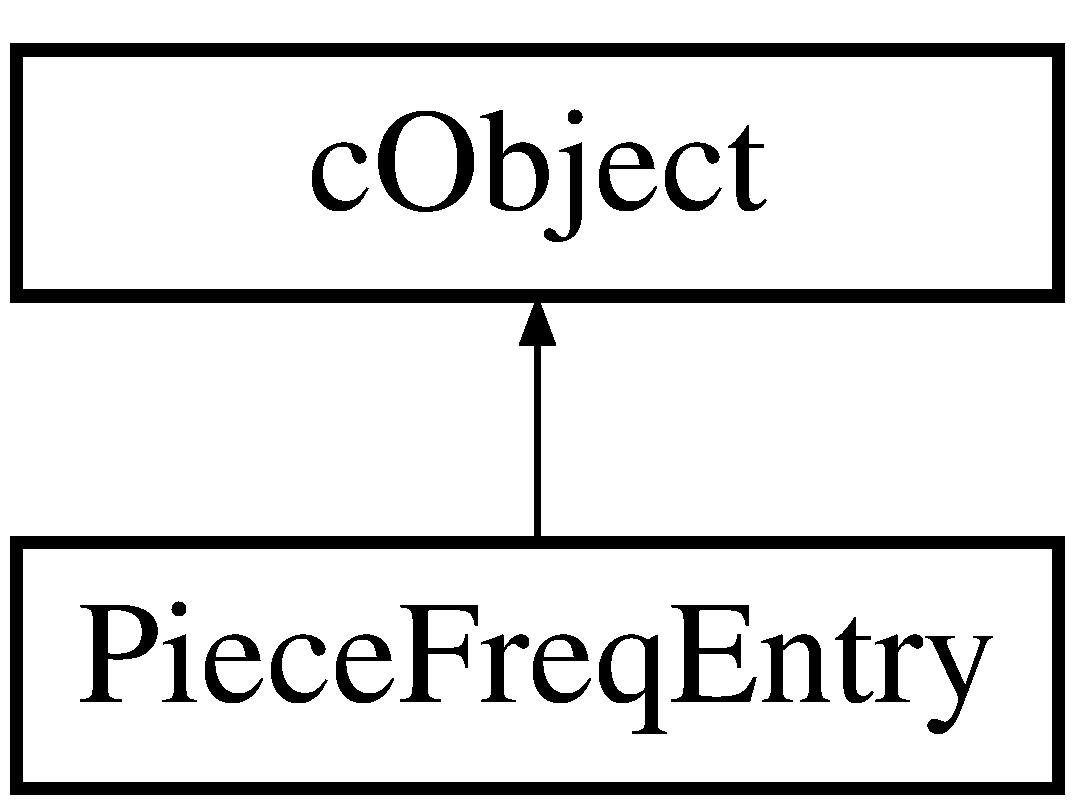
\includegraphics[height=2.000000cm]{classPieceFreqEntry}
\end{center}
\end{figure}
\subsection*{Public Member Functions}
\begin{DoxyCompactItemize}
\item 
\hyperlink{classPieceFreqEntry_a0e464a4934e49f90efcfa802bfa7fdf6}{Piece\+Freq\+Entry} ()
\item 
\hyperlink{classPieceFreqEntry_adafb0be76054575c5f14236ecd32b4fe}{Piece\+Freq\+Entry} (int, int)
\item 
\hyperlink{classPieceFreqEntry_ab2d463151a3da40dc28e6a689394ffc9}{Piece\+Freq\+Entry} (const \hyperlink{classPieceFreqEntry}{Piece\+Freq\+Entry} \&)
\item 
virtual \hyperlink{classPieceFreqEntry_a6a5abb3209e9378fe5e5517ccea608fc}{$\sim$\+Piece\+Freq\+Entry} ()
\item 
int \hyperlink{classPieceFreqEntry_a7ff67106af5a5c461aae6b6a715522f0}{get\+Index} ()
\item 
void \hyperlink{classPieceFreqEntry_a6bdabb68a3d55489e08f7d3ff890bc74}{set\+Index} (int)
\item 
int \hyperlink{classPieceFreqEntry_af99f1ee99558ca892e0970f7c82d34c5}{frequency} ()
\item 
void \hyperlink{classPieceFreqEntry_a2d8c5fa9352de498474563fabffa6bd7}{set\+Frequency} (int)
\item 
bool \hyperlink{classPieceFreqEntry_ab31f7040904772302581553cea97a293}{operator$<$} (const \hyperlink{classPieceFreqEntry}{Piece\+Freq\+Entry} \&item) const 
\item 
void \hyperlink{classPieceFreqEntry_adf78afa1bb62e20274d18b216a960def}{operator=} (const \hyperlink{classPieceFreqEntry}{Piece\+Freq\+Entry} \&item)
\item 
void \hyperlink{classPieceFreqEntry_adbb5d3599d155b18050b1ac3cbc4d6a1}{operator++} (int)
\item 
void \hyperlink{classPieceFreqEntry_af209878df02faeea7cb2b9949f916a2d}{operator+=} (int)
\end{DoxyCompactItemize}
\subsection*{Protected Attributes}
\begin{DoxyCompactItemize}
\item 
int \hyperlink{classPieceFreqEntry_afa218e86efc8383f929ece6de321c24c}{index\+\_\+var}
\item 
int \hyperlink{classPieceFreqEntry_ae2273456e6dacc5c5e691143a525d349}{frequency\+\_\+var}
\end{DoxyCompactItemize}


\subsection{Constructor \& Destructor Documentation}
\hypertarget{classPieceFreqEntry_a0e464a4934e49f90efcfa802bfa7fdf6}{}\index{Piece\+Freq\+Entry@{Piece\+Freq\+Entry}!Piece\+Freq\+Entry@{Piece\+Freq\+Entry}}
\index{Piece\+Freq\+Entry@{Piece\+Freq\+Entry}!Piece\+Freq\+Entry@{Piece\+Freq\+Entry}}
\subsubsection[{Piece\+Freq\+Entry()}]{\setlength{\rightskip}{0pt plus 5cm}Piece\+Freq\+Entry\+::\+Piece\+Freq\+Entry (
\begin{DoxyParamCaption}
{}
\end{DoxyParamCaption}
)}\label{classPieceFreqEntry_a0e464a4934e49f90efcfa802bfa7fdf6}
\hypertarget{classPieceFreqEntry_adafb0be76054575c5f14236ecd32b4fe}{}\index{Piece\+Freq\+Entry@{Piece\+Freq\+Entry}!Piece\+Freq\+Entry@{Piece\+Freq\+Entry}}
\index{Piece\+Freq\+Entry@{Piece\+Freq\+Entry}!Piece\+Freq\+Entry@{Piece\+Freq\+Entry}}
\subsubsection[{Piece\+Freq\+Entry(int, int)}]{\setlength{\rightskip}{0pt plus 5cm}Piece\+Freq\+Entry\+::\+Piece\+Freq\+Entry (
\begin{DoxyParamCaption}
\item[{int}]{i, }
\item[{int}]{f}
\end{DoxyParamCaption}
)}\label{classPieceFreqEntry_adafb0be76054575c5f14236ecd32b4fe}
\hypertarget{classPieceFreqEntry_ab2d463151a3da40dc28e6a689394ffc9}{}\index{Piece\+Freq\+Entry@{Piece\+Freq\+Entry}!Piece\+Freq\+Entry@{Piece\+Freq\+Entry}}
\index{Piece\+Freq\+Entry@{Piece\+Freq\+Entry}!Piece\+Freq\+Entry@{Piece\+Freq\+Entry}}
\subsubsection[{Piece\+Freq\+Entry(const Piece\+Freq\+Entry \&)}]{\setlength{\rightskip}{0pt plus 5cm}Piece\+Freq\+Entry\+::\+Piece\+Freq\+Entry (
\begin{DoxyParamCaption}
\item[{const {\bf Piece\+Freq\+Entry} \&}]{cp}
\end{DoxyParamCaption}
)}\label{classPieceFreqEntry_ab2d463151a3da40dc28e6a689394ffc9}
\hypertarget{classPieceFreqEntry_a6a5abb3209e9378fe5e5517ccea608fc}{}\index{Piece\+Freq\+Entry@{Piece\+Freq\+Entry}!````~Piece\+Freq\+Entry@{$\sim$\+Piece\+Freq\+Entry}}
\index{````~Piece\+Freq\+Entry@{$\sim$\+Piece\+Freq\+Entry}!Piece\+Freq\+Entry@{Piece\+Freq\+Entry}}
\subsubsection[{$\sim$\+Piece\+Freq\+Entry()}]{\setlength{\rightskip}{0pt plus 5cm}Piece\+Freq\+Entry\+::$\sim$\+Piece\+Freq\+Entry (
\begin{DoxyParamCaption}
{}
\end{DoxyParamCaption}
)\hspace{0.3cm}{\ttfamily [virtual]}}\label{classPieceFreqEntry_a6a5abb3209e9378fe5e5517ccea608fc}


\subsection{Member Function Documentation}
\hypertarget{classPieceFreqEntry_af99f1ee99558ca892e0970f7c82d34c5}{}\index{Piece\+Freq\+Entry@{Piece\+Freq\+Entry}!frequency@{frequency}}
\index{frequency@{frequency}!Piece\+Freq\+Entry@{Piece\+Freq\+Entry}}
\subsubsection[{frequency()}]{\setlength{\rightskip}{0pt plus 5cm}int Piece\+Freq\+Entry\+::frequency (
\begin{DoxyParamCaption}
{}
\end{DoxyParamCaption}
)}\label{classPieceFreqEntry_af99f1ee99558ca892e0970f7c82d34c5}
\hypertarget{classPieceFreqEntry_a7ff67106af5a5c461aae6b6a715522f0}{}\index{Piece\+Freq\+Entry@{Piece\+Freq\+Entry}!get\+Index@{get\+Index}}
\index{get\+Index@{get\+Index}!Piece\+Freq\+Entry@{Piece\+Freq\+Entry}}
\subsubsection[{get\+Index()}]{\setlength{\rightskip}{0pt plus 5cm}int Piece\+Freq\+Entry\+::get\+Index (
\begin{DoxyParamCaption}
{}
\end{DoxyParamCaption}
)}\label{classPieceFreqEntry_a7ff67106af5a5c461aae6b6a715522f0}
\hypertarget{classPieceFreqEntry_adbb5d3599d155b18050b1ac3cbc4d6a1}{}\index{Piece\+Freq\+Entry@{Piece\+Freq\+Entry}!operator++@{operator++}}
\index{operator++@{operator++}!Piece\+Freq\+Entry@{Piece\+Freq\+Entry}}
\subsubsection[{operator++(int)}]{\setlength{\rightskip}{0pt plus 5cm}void Piece\+Freq\+Entry\+::operator++ (
\begin{DoxyParamCaption}
\item[{int}]{}
\end{DoxyParamCaption}
)}\label{classPieceFreqEntry_adbb5d3599d155b18050b1ac3cbc4d6a1}
\hypertarget{classPieceFreqEntry_af209878df02faeea7cb2b9949f916a2d}{}\index{Piece\+Freq\+Entry@{Piece\+Freq\+Entry}!operator+=@{operator+=}}
\index{operator+=@{operator+=}!Piece\+Freq\+Entry@{Piece\+Freq\+Entry}}
\subsubsection[{operator+=(int)}]{\setlength{\rightskip}{0pt plus 5cm}void Piece\+Freq\+Entry\+::operator+= (
\begin{DoxyParamCaption}
\item[{int}]{i}
\end{DoxyParamCaption}
)}\label{classPieceFreqEntry_af209878df02faeea7cb2b9949f916a2d}
\hypertarget{classPieceFreqEntry_ab31f7040904772302581553cea97a293}{}\index{Piece\+Freq\+Entry@{Piece\+Freq\+Entry}!operator$<$@{operator$<$}}
\index{operator$<$@{operator$<$}!Piece\+Freq\+Entry@{Piece\+Freq\+Entry}}
\subsubsection[{operator$<$(const Piece\+Freq\+Entry \&item) const }]{\setlength{\rightskip}{0pt plus 5cm}bool Piece\+Freq\+Entry\+::operator$<$ (
\begin{DoxyParamCaption}
\item[{const {\bf Piece\+Freq\+Entry} \&}]{item}
\end{DoxyParamCaption}
) const}\label{classPieceFreqEntry_ab31f7040904772302581553cea97a293}
\hypertarget{classPieceFreqEntry_adf78afa1bb62e20274d18b216a960def}{}\index{Piece\+Freq\+Entry@{Piece\+Freq\+Entry}!operator=@{operator=}}
\index{operator=@{operator=}!Piece\+Freq\+Entry@{Piece\+Freq\+Entry}}
\subsubsection[{operator=(const Piece\+Freq\+Entry \&item)}]{\setlength{\rightskip}{0pt plus 5cm}void Piece\+Freq\+Entry\+::operator= (
\begin{DoxyParamCaption}
\item[{const {\bf Piece\+Freq\+Entry} \&}]{item}
\end{DoxyParamCaption}
)}\label{classPieceFreqEntry_adf78afa1bb62e20274d18b216a960def}
\hypertarget{classPieceFreqEntry_a2d8c5fa9352de498474563fabffa6bd7}{}\index{Piece\+Freq\+Entry@{Piece\+Freq\+Entry}!set\+Frequency@{set\+Frequency}}
\index{set\+Frequency@{set\+Frequency}!Piece\+Freq\+Entry@{Piece\+Freq\+Entry}}
\subsubsection[{set\+Frequency(int)}]{\setlength{\rightskip}{0pt plus 5cm}void Piece\+Freq\+Entry\+::set\+Frequency (
\begin{DoxyParamCaption}
\item[{int}]{f}
\end{DoxyParamCaption}
)}\label{classPieceFreqEntry_a2d8c5fa9352de498474563fabffa6bd7}
\hypertarget{classPieceFreqEntry_a6bdabb68a3d55489e08f7d3ff890bc74}{}\index{Piece\+Freq\+Entry@{Piece\+Freq\+Entry}!set\+Index@{set\+Index}}
\index{set\+Index@{set\+Index}!Piece\+Freq\+Entry@{Piece\+Freq\+Entry}}
\subsubsection[{set\+Index(int)}]{\setlength{\rightskip}{0pt plus 5cm}void Piece\+Freq\+Entry\+::set\+Index (
\begin{DoxyParamCaption}
\item[{int}]{i}
\end{DoxyParamCaption}
)}\label{classPieceFreqEntry_a6bdabb68a3d55489e08f7d3ff890bc74}


\subsection{Member Data Documentation}
\hypertarget{classPieceFreqEntry_ae2273456e6dacc5c5e691143a525d349}{}\index{Piece\+Freq\+Entry@{Piece\+Freq\+Entry}!frequency\+\_\+var@{frequency\+\_\+var}}
\index{frequency\+\_\+var@{frequency\+\_\+var}!Piece\+Freq\+Entry@{Piece\+Freq\+Entry}}
\subsubsection[{frequency\+\_\+var}]{\setlength{\rightskip}{0pt plus 5cm}int Piece\+Freq\+Entry\+::frequency\+\_\+var\hspace{0.3cm}{\ttfamily [protected]}}\label{classPieceFreqEntry_ae2273456e6dacc5c5e691143a525d349}
\hypertarget{classPieceFreqEntry_afa218e86efc8383f929ece6de321c24c}{}\index{Piece\+Freq\+Entry@{Piece\+Freq\+Entry}!index\+\_\+var@{index\+\_\+var}}
\index{index\+\_\+var@{index\+\_\+var}!Piece\+Freq\+Entry@{Piece\+Freq\+Entry}}
\subsubsection[{index\+\_\+var}]{\setlength{\rightskip}{0pt plus 5cm}int Piece\+Freq\+Entry\+::index\+\_\+var\hspace{0.3cm}{\ttfamily [protected]}}\label{classPieceFreqEntry_afa218e86efc8383f929ece6de321c24c}


The documentation for this class was generated from the following files\+:\begin{DoxyCompactItemize}
\item 
\hyperlink{BTUtils_8h}{B\+T\+Utils.\+h}\item 
\hyperlink{BTUtils_8cc}{B\+T\+Utils.\+cc}\end{DoxyCompactItemize}

\hypertarget{classPieceFreqState}{}\section{Piece\+Freq\+State Class Reference}
\label{classPieceFreqState}\index{Piece\+Freq\+State@{Piece\+Freq\+State}}


{\ttfamily \#include $<$B\+T\+Utils.\+h$>$}

\subsection*{Public Member Functions}
\begin{DoxyCompactItemize}
\item 
void \hyperlink{classPieceFreqState_a945dd89d1b0df6767817d34b4d788955}{initialize\+Piece\+Frequencies} (int num\+Of\+Pieces)
\item 
void \hyperlink{classPieceFreqState_a711cdb21b1bd02659085f86fd58fc855}{print\+Piece\+Frequencies} ()
\item 
void \hyperlink{classPieceFreqState_a8abf2288dfad8b229dbd4eaa56025ee4}{increase\+Piece\+Frequency} (int index)
\item 
\hyperlink{BTUtils_8h_a93815334b34fe6744f67a8609bec0eaf}{Piece\+Freq\+Entry\+Vector} \hyperlink{classPieceFreqState_a9939e3c457da806a38ce7c7a4bc770a7}{get\+Vector} ()
\item 
void \hyperlink{classPieceFreqState_ac103a1963dfa2dec5b2c8a94297d6669}{update\+Piece\+Frequencies} (\hyperlink{classBTBitfieldMsg}{B\+T\+Bitfield\+Msg} $\ast$)
\item 
void \hyperlink{classPieceFreqState_ad735f08b52e580f2ab46fee92ff31211}{clear} ()
\end{DoxyCompactItemize}
\subsection*{Protected Attributes}
\begin{DoxyCompactItemize}
\item 
\hyperlink{BTUtils_8h_a93815334b34fe6744f67a8609bec0eaf}{Piece\+Freq\+Entry\+Vector} \hyperlink{classPieceFreqState_a14a8a32e47ebdc5e9522739e10cbfb28}{piece\+Freq\+Vector}
\end{DoxyCompactItemize}


\subsection{Member Function Documentation}
\hypertarget{classPieceFreqState_ad735f08b52e580f2ab46fee92ff31211}{}\index{Piece\+Freq\+State@{Piece\+Freq\+State}!clear@{clear}}
\index{clear@{clear}!Piece\+Freq\+State@{Piece\+Freq\+State}}
\subsubsection[{clear()}]{\setlength{\rightskip}{0pt plus 5cm}void Piece\+Freq\+State\+::clear (
\begin{DoxyParamCaption}
{}
\end{DoxyParamCaption}
)}\label{classPieceFreqState_ad735f08b52e580f2ab46fee92ff31211}
\hypertarget{classPieceFreqState_a9939e3c457da806a38ce7c7a4bc770a7}{}\index{Piece\+Freq\+State@{Piece\+Freq\+State}!get\+Vector@{get\+Vector}}
\index{get\+Vector@{get\+Vector}!Piece\+Freq\+State@{Piece\+Freq\+State}}
\subsubsection[{get\+Vector()}]{\setlength{\rightskip}{0pt plus 5cm}{\bf Piece\+Freq\+Entry\+Vector} Piece\+Freq\+State\+::get\+Vector (
\begin{DoxyParamCaption}
{}
\end{DoxyParamCaption}
)}\label{classPieceFreqState_a9939e3c457da806a38ce7c7a4bc770a7}
\hypertarget{classPieceFreqState_a8abf2288dfad8b229dbd4eaa56025ee4}{}\index{Piece\+Freq\+State@{Piece\+Freq\+State}!increase\+Piece\+Frequency@{increase\+Piece\+Frequency}}
\index{increase\+Piece\+Frequency@{increase\+Piece\+Frequency}!Piece\+Freq\+State@{Piece\+Freq\+State}}
\subsubsection[{increase\+Piece\+Frequency(int index)}]{\setlength{\rightskip}{0pt plus 5cm}void Piece\+Freq\+State\+::increase\+Piece\+Frequency (
\begin{DoxyParamCaption}
\item[{int}]{index}
\end{DoxyParamCaption}
)}\label{classPieceFreqState_a8abf2288dfad8b229dbd4eaa56025ee4}
\hypertarget{classPieceFreqState_a945dd89d1b0df6767817d34b4d788955}{}\index{Piece\+Freq\+State@{Piece\+Freq\+State}!initialize\+Piece\+Frequencies@{initialize\+Piece\+Frequencies}}
\index{initialize\+Piece\+Frequencies@{initialize\+Piece\+Frequencies}!Piece\+Freq\+State@{Piece\+Freq\+State}}
\subsubsection[{initialize\+Piece\+Frequencies(int num\+Of\+Pieces)}]{\setlength{\rightskip}{0pt plus 5cm}void Piece\+Freq\+State\+::initialize\+Piece\+Frequencies (
\begin{DoxyParamCaption}
\item[{int}]{num\+Of\+Pieces}
\end{DoxyParamCaption}
)}\label{classPieceFreqState_a945dd89d1b0df6767817d34b4d788955}
\hypertarget{classPieceFreqState_a711cdb21b1bd02659085f86fd58fc855}{}\index{Piece\+Freq\+State@{Piece\+Freq\+State}!print\+Piece\+Frequencies@{print\+Piece\+Frequencies}}
\index{print\+Piece\+Frequencies@{print\+Piece\+Frequencies}!Piece\+Freq\+State@{Piece\+Freq\+State}}
\subsubsection[{print\+Piece\+Frequencies()}]{\setlength{\rightskip}{0pt plus 5cm}void Piece\+Freq\+State\+::print\+Piece\+Frequencies (
\begin{DoxyParamCaption}
{}
\end{DoxyParamCaption}
)}\label{classPieceFreqState_a711cdb21b1bd02659085f86fd58fc855}
\hypertarget{classPieceFreqState_ac103a1963dfa2dec5b2c8a94297d6669}{}\index{Piece\+Freq\+State@{Piece\+Freq\+State}!update\+Piece\+Frequencies@{update\+Piece\+Frequencies}}
\index{update\+Piece\+Frequencies@{update\+Piece\+Frequencies}!Piece\+Freq\+State@{Piece\+Freq\+State}}
\subsubsection[{update\+Piece\+Frequencies(\+B\+T\+Bitfield\+Msg $\ast$)}]{\setlength{\rightskip}{0pt plus 5cm}void Piece\+Freq\+State\+::update\+Piece\+Frequencies (
\begin{DoxyParamCaption}
\item[{{\bf B\+T\+Bitfield\+Msg} $\ast$}]{msg}
\end{DoxyParamCaption}
)}\label{classPieceFreqState_ac103a1963dfa2dec5b2c8a94297d6669}


\subsection{Member Data Documentation}
\hypertarget{classPieceFreqState_a14a8a32e47ebdc5e9522739e10cbfb28}{}\index{Piece\+Freq\+State@{Piece\+Freq\+State}!piece\+Freq\+Vector@{piece\+Freq\+Vector}}
\index{piece\+Freq\+Vector@{piece\+Freq\+Vector}!Piece\+Freq\+State@{Piece\+Freq\+State}}
\subsubsection[{piece\+Freq\+Vector}]{\setlength{\rightskip}{0pt plus 5cm}{\bf Piece\+Freq\+Entry\+Vector} Piece\+Freq\+State\+::piece\+Freq\+Vector\hspace{0.3cm}{\ttfamily [protected]}}\label{classPieceFreqState_a14a8a32e47ebdc5e9522739e10cbfb28}


The documentation for this class was generated from the following files\+:\begin{DoxyCompactItemize}
\item 
\hyperlink{BTUtils_8h}{B\+T\+Utils.\+h}\item 
\hyperlink{BTUtils_8cc}{B\+T\+Utils.\+cc}\end{DoxyCompactItemize}

\hypertarget{classRequestEntry}{}\section{Request\+Entry Class Reference}
\label{classRequestEntry}\index{Request\+Entry@{Request\+Entry}}


{\ttfamily \#include $<$B\+T\+Utils.\+h$>$}

Inheritance diagram for Request\+Entry\+:\begin{figure}[H]
\begin{center}
\leavevmode
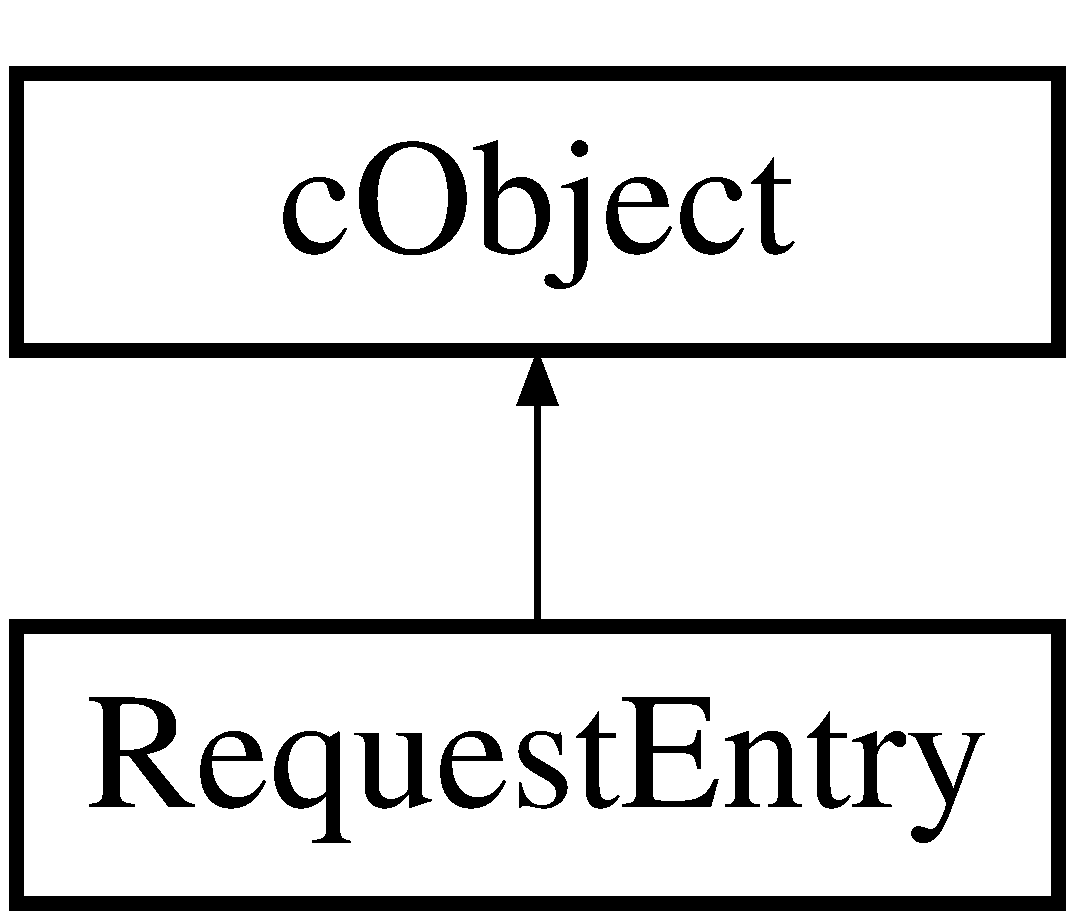
\includegraphics[height=2.000000cm]{classRequestEntry}
\end{center}
\end{figure}
\subsection*{Public Member Functions}
\begin{DoxyCompactItemize}
\item 
\hyperlink{classRequestEntry_a95d45a84e3e25909c5b065450bad4aad}{Request\+Entry} ()
\item 
\hyperlink{classRequestEntry_a69b1396e2e503cc704a3cf9157ca24e8}{Request\+Entry} (int, int, int, simtime\+\_\+t, const char $\ast$, httpt\+Base\+Message $\ast$)
\item 
\hyperlink{classRequestEntry_a85528d356b3ee23388b0297accb7fd12}{Request\+Entry} (const \hyperlink{classRequestEntry}{Request\+Entry} \&)
\item 
virtual \hyperlink{classRequestEntry_ab26a3ee47c31028f6771ed54e66fae28}{$\sim$\+Request\+Entry} ()
\item 
int \hyperlink{classRequestEntry_afb1e573d37bbf1cce5b20b6162c595c8}{get\+Index} ()
\item 
void \hyperlink{classRequestEntry_abe544acc9da02db6c8d4f35464097167}{set\+Index} (int)
\item 
int \hyperlink{classRequestEntry_afc8ad0d9147c91db24dcf92806d8e936}{begin} ()
\item 
void \hyperlink{classRequestEntry_a97d3640f9e93745f8356865e69a1bb48}{set\+Begin} (int)
\item 
int \hyperlink{classRequestEntry_a74e4135e2270898733bf8f0c5fcae8da}{length} ()
\item 
void \hyperlink{classRequestEntry_aacf772652f33c8dc3c8655dc3bb02c85}{set\+Bit\+Length} (int)
\item 
simtime\+\_\+t \hyperlink{classRequestEntry_a71cec14c796056ae048e669617239a40}{get\+Timestamp} ()
\item 
void \hyperlink{classRequestEntry_a89e2cf2af0520908c2f778eeba4ca8a4}{set\+Timestamp} (simtime\+\_\+t)
\item 
const char $\ast$ \hyperlink{classRequestEntry_a469a3d7a9242f3cbc3b9a5279782045a}{peer\+I\+D} ()
\item 
void \hyperlink{classRequestEntry_ad3a725cd00fd5e86db33a490fdfdc860}{set\+Peer\+I\+D} (const char $\ast$)
\item 
httpt\+Base\+Message $\ast$ \hyperlink{classRequestEntry_aa78d3b3d332bc540fd949a572a6b0252}{http\+Reply\+Message} ()
\item 
void \hyperlink{classRequestEntry_a5fa7c81c38d3a96918784090d73112c8}{set\+Http\+Reply\+Message} (httpt\+Base\+Message $\ast$)
\item 
\hyperlink{classRequestEntry}{Request\+Entry} \hyperlink{classRequestEntry_ad783916b2da98cd5e2e7cfea32eb72f6}{dup} ()
\end{DoxyCompactItemize}
\subsection*{Protected Attributes}
\begin{DoxyCompactItemize}
\item 
int \hyperlink{classRequestEntry_a8ab0e52289f7c8e9cff73de49bf3c7c3}{index\+\_\+var}
\item 
int \hyperlink{classRequestEntry_ad50fcc4c262ffae45bbd745e6371a472}{begin\+\_\+var}
\item 
int \hyperlink{classRequestEntry_aa52549120084c3fccd2101678e84c6fe}{length\+\_\+var}
\item 
simtime\+\_\+t \hyperlink{classRequestEntry_aeb81ed7dd1b44291051176524448c7c9}{timestamp\+\_\+var}
\item 
const char $\ast$ \hyperlink{classRequestEntry_a0b527dea15dd777cd9267ab9bc5ccdc2}{peer\+I\+D\+\_\+var}
\item 
httpt\+Base\+Message $\ast$ \hyperlink{classRequestEntry_a515e817884d92935dfaf47320aa1a47b}{http\+Reply\+\_\+var}
\end{DoxyCompactItemize}


\subsection{Constructor \& Destructor Documentation}
\hypertarget{classRequestEntry_a95d45a84e3e25909c5b065450bad4aad}{}\index{Request\+Entry@{Request\+Entry}!Request\+Entry@{Request\+Entry}}
\index{Request\+Entry@{Request\+Entry}!Request\+Entry@{Request\+Entry}}
\subsubsection[{Request\+Entry()}]{\setlength{\rightskip}{0pt plus 5cm}Request\+Entry\+::\+Request\+Entry (
\begin{DoxyParamCaption}
{}
\end{DoxyParamCaption}
)}\label{classRequestEntry_a95d45a84e3e25909c5b065450bad4aad}
\hypertarget{classRequestEntry_a69b1396e2e503cc704a3cf9157ca24e8}{}\index{Request\+Entry@{Request\+Entry}!Request\+Entry@{Request\+Entry}}
\index{Request\+Entry@{Request\+Entry}!Request\+Entry@{Request\+Entry}}
\subsubsection[{Request\+Entry(int, int, int, simtime\+\_\+t, const char $\ast$, httpt\+Base\+Message $\ast$)}]{\setlength{\rightskip}{0pt plus 5cm}Request\+Entry\+::\+Request\+Entry (
\begin{DoxyParamCaption}
\item[{int}]{i, }
\item[{int}]{b, }
\item[{int}]{l, }
\item[{simtime\+\_\+t}]{t, }
\item[{const char $\ast$}]{id, }
\item[{httpt\+Base\+Message $\ast$}]{http\+Reply}
\end{DoxyParamCaption}
)}\label{classRequestEntry_a69b1396e2e503cc704a3cf9157ca24e8}
\hypertarget{classRequestEntry_a85528d356b3ee23388b0297accb7fd12}{}\index{Request\+Entry@{Request\+Entry}!Request\+Entry@{Request\+Entry}}
\index{Request\+Entry@{Request\+Entry}!Request\+Entry@{Request\+Entry}}
\subsubsection[{Request\+Entry(const Request\+Entry \&)}]{\setlength{\rightskip}{0pt plus 5cm}Request\+Entry\+::\+Request\+Entry (
\begin{DoxyParamCaption}
\item[{const {\bf Request\+Entry} \&}]{re}
\end{DoxyParamCaption}
)}\label{classRequestEntry_a85528d356b3ee23388b0297accb7fd12}
\hypertarget{classRequestEntry_ab26a3ee47c31028f6771ed54e66fae28}{}\index{Request\+Entry@{Request\+Entry}!````~Request\+Entry@{$\sim$\+Request\+Entry}}
\index{````~Request\+Entry@{$\sim$\+Request\+Entry}!Request\+Entry@{Request\+Entry}}
\subsubsection[{$\sim$\+Request\+Entry()}]{\setlength{\rightskip}{0pt plus 5cm}Request\+Entry\+::$\sim$\+Request\+Entry (
\begin{DoxyParamCaption}
{}
\end{DoxyParamCaption}
)\hspace{0.3cm}{\ttfamily [virtual]}}\label{classRequestEntry_ab26a3ee47c31028f6771ed54e66fae28}


\subsection{Member Function Documentation}
\hypertarget{classRequestEntry_afc8ad0d9147c91db24dcf92806d8e936}{}\index{Request\+Entry@{Request\+Entry}!begin@{begin}}
\index{begin@{begin}!Request\+Entry@{Request\+Entry}}
\subsubsection[{begin()}]{\setlength{\rightskip}{0pt plus 5cm}int Request\+Entry\+::begin (
\begin{DoxyParamCaption}
{}
\end{DoxyParamCaption}
)}\label{classRequestEntry_afc8ad0d9147c91db24dcf92806d8e936}
\hypertarget{classRequestEntry_ad783916b2da98cd5e2e7cfea32eb72f6}{}\index{Request\+Entry@{Request\+Entry}!dup@{dup}}
\index{dup@{dup}!Request\+Entry@{Request\+Entry}}
\subsubsection[{dup()}]{\setlength{\rightskip}{0pt plus 5cm}{\bf Request\+Entry} Request\+Entry\+::dup (
\begin{DoxyParamCaption}
{}
\end{DoxyParamCaption}
)}\label{classRequestEntry_ad783916b2da98cd5e2e7cfea32eb72f6}
\hypertarget{classRequestEntry_afb1e573d37bbf1cce5b20b6162c595c8}{}\index{Request\+Entry@{Request\+Entry}!get\+Index@{get\+Index}}
\index{get\+Index@{get\+Index}!Request\+Entry@{Request\+Entry}}
\subsubsection[{get\+Index()}]{\setlength{\rightskip}{0pt plus 5cm}int Request\+Entry\+::get\+Index (
\begin{DoxyParamCaption}
{}
\end{DoxyParamCaption}
)}\label{classRequestEntry_afb1e573d37bbf1cce5b20b6162c595c8}
\hypertarget{classRequestEntry_a71cec14c796056ae048e669617239a40}{}\index{Request\+Entry@{Request\+Entry}!get\+Timestamp@{get\+Timestamp}}
\index{get\+Timestamp@{get\+Timestamp}!Request\+Entry@{Request\+Entry}}
\subsubsection[{get\+Timestamp()}]{\setlength{\rightskip}{0pt plus 5cm}simtime\+\_\+t Request\+Entry\+::get\+Timestamp (
\begin{DoxyParamCaption}
{}
\end{DoxyParamCaption}
)}\label{classRequestEntry_a71cec14c796056ae048e669617239a40}
\hypertarget{classRequestEntry_aa78d3b3d332bc540fd949a572a6b0252}{}\index{Request\+Entry@{Request\+Entry}!http\+Reply\+Message@{http\+Reply\+Message}}
\index{http\+Reply\+Message@{http\+Reply\+Message}!Request\+Entry@{Request\+Entry}}
\subsubsection[{http\+Reply\+Message()}]{\setlength{\rightskip}{0pt plus 5cm}httpt\+Base\+Message $\ast$ Request\+Entry\+::http\+Reply\+Message (
\begin{DoxyParamCaption}
{}
\end{DoxyParamCaption}
)}\label{classRequestEntry_aa78d3b3d332bc540fd949a572a6b0252}
\hypertarget{classRequestEntry_a74e4135e2270898733bf8f0c5fcae8da}{}\index{Request\+Entry@{Request\+Entry}!length@{length}}
\index{length@{length}!Request\+Entry@{Request\+Entry}}
\subsubsection[{length()}]{\setlength{\rightskip}{0pt plus 5cm}int Request\+Entry\+::length (
\begin{DoxyParamCaption}
{}
\end{DoxyParamCaption}
)}\label{classRequestEntry_a74e4135e2270898733bf8f0c5fcae8da}
\hypertarget{classRequestEntry_a469a3d7a9242f3cbc3b9a5279782045a}{}\index{Request\+Entry@{Request\+Entry}!peer\+I\+D@{peer\+I\+D}}
\index{peer\+I\+D@{peer\+I\+D}!Request\+Entry@{Request\+Entry}}
\subsubsection[{peer\+I\+D()}]{\setlength{\rightskip}{0pt plus 5cm}const char $\ast$ Request\+Entry\+::peer\+I\+D (
\begin{DoxyParamCaption}
{}
\end{DoxyParamCaption}
)}\label{classRequestEntry_a469a3d7a9242f3cbc3b9a5279782045a}
\hypertarget{classRequestEntry_a97d3640f9e93745f8356865e69a1bb48}{}\index{Request\+Entry@{Request\+Entry}!set\+Begin@{set\+Begin}}
\index{set\+Begin@{set\+Begin}!Request\+Entry@{Request\+Entry}}
\subsubsection[{set\+Begin(int)}]{\setlength{\rightskip}{0pt plus 5cm}void Request\+Entry\+::set\+Begin (
\begin{DoxyParamCaption}
\item[{int}]{b}
\end{DoxyParamCaption}
)}\label{classRequestEntry_a97d3640f9e93745f8356865e69a1bb48}
\hypertarget{classRequestEntry_aacf772652f33c8dc3c8655dc3bb02c85}{}\index{Request\+Entry@{Request\+Entry}!set\+Bit\+Length@{set\+Bit\+Length}}
\index{set\+Bit\+Length@{set\+Bit\+Length}!Request\+Entry@{Request\+Entry}}
\subsubsection[{set\+Bit\+Length(int)}]{\setlength{\rightskip}{0pt plus 5cm}void Request\+Entry\+::set\+Bit\+Length (
\begin{DoxyParamCaption}
\item[{int}]{l}
\end{DoxyParamCaption}
)}\label{classRequestEntry_aacf772652f33c8dc3c8655dc3bb02c85}
\hypertarget{classRequestEntry_a5fa7c81c38d3a96918784090d73112c8}{}\index{Request\+Entry@{Request\+Entry}!set\+Http\+Reply\+Message@{set\+Http\+Reply\+Message}}
\index{set\+Http\+Reply\+Message@{set\+Http\+Reply\+Message}!Request\+Entry@{Request\+Entry}}
\subsubsection[{set\+Http\+Reply\+Message(httpt\+Base\+Message $\ast$)}]{\setlength{\rightskip}{0pt plus 5cm}void Request\+Entry\+::set\+Http\+Reply\+Message (
\begin{DoxyParamCaption}
\item[{httpt\+Base\+Message $\ast$}]{http\+Reply}
\end{DoxyParamCaption}
)}\label{classRequestEntry_a5fa7c81c38d3a96918784090d73112c8}
\hypertarget{classRequestEntry_abe544acc9da02db6c8d4f35464097167}{}\index{Request\+Entry@{Request\+Entry}!set\+Index@{set\+Index}}
\index{set\+Index@{set\+Index}!Request\+Entry@{Request\+Entry}}
\subsubsection[{set\+Index(int)}]{\setlength{\rightskip}{0pt plus 5cm}void Request\+Entry\+::set\+Index (
\begin{DoxyParamCaption}
\item[{int}]{i}
\end{DoxyParamCaption}
)}\label{classRequestEntry_abe544acc9da02db6c8d4f35464097167}
\hypertarget{classRequestEntry_ad3a725cd00fd5e86db33a490fdfdc860}{}\index{Request\+Entry@{Request\+Entry}!set\+Peer\+I\+D@{set\+Peer\+I\+D}}
\index{set\+Peer\+I\+D@{set\+Peer\+I\+D}!Request\+Entry@{Request\+Entry}}
\subsubsection[{set\+Peer\+I\+D(const char $\ast$)}]{\setlength{\rightskip}{0pt plus 5cm}void Request\+Entry\+::set\+Peer\+I\+D (
\begin{DoxyParamCaption}
\item[{const char $\ast$}]{id}
\end{DoxyParamCaption}
)}\label{classRequestEntry_ad3a725cd00fd5e86db33a490fdfdc860}
\hypertarget{classRequestEntry_a89e2cf2af0520908c2f778eeba4ca8a4}{}\index{Request\+Entry@{Request\+Entry}!set\+Timestamp@{set\+Timestamp}}
\index{set\+Timestamp@{set\+Timestamp}!Request\+Entry@{Request\+Entry}}
\subsubsection[{set\+Timestamp(simtime\+\_\+t)}]{\setlength{\rightskip}{0pt plus 5cm}void Request\+Entry\+::set\+Timestamp (
\begin{DoxyParamCaption}
\item[{simtime\+\_\+t}]{timestamp}
\end{DoxyParamCaption}
)}\label{classRequestEntry_a89e2cf2af0520908c2f778eeba4ca8a4}


\subsection{Member Data Documentation}
\hypertarget{classRequestEntry_ad50fcc4c262ffae45bbd745e6371a472}{}\index{Request\+Entry@{Request\+Entry}!begin\+\_\+var@{begin\+\_\+var}}
\index{begin\+\_\+var@{begin\+\_\+var}!Request\+Entry@{Request\+Entry}}
\subsubsection[{begin\+\_\+var}]{\setlength{\rightskip}{0pt plus 5cm}int Request\+Entry\+::begin\+\_\+var\hspace{0.3cm}{\ttfamily [protected]}}\label{classRequestEntry_ad50fcc4c262ffae45bbd745e6371a472}
\hypertarget{classRequestEntry_a515e817884d92935dfaf47320aa1a47b}{}\index{Request\+Entry@{Request\+Entry}!http\+Reply\+\_\+var@{http\+Reply\+\_\+var}}
\index{http\+Reply\+\_\+var@{http\+Reply\+\_\+var}!Request\+Entry@{Request\+Entry}}
\subsubsection[{http\+Reply\+\_\+var}]{\setlength{\rightskip}{0pt plus 5cm}httpt\+Base\+Message$\ast$ Request\+Entry\+::http\+Reply\+\_\+var\hspace{0.3cm}{\ttfamily [protected]}}\label{classRequestEntry_a515e817884d92935dfaf47320aa1a47b}
\hypertarget{classRequestEntry_a8ab0e52289f7c8e9cff73de49bf3c7c3}{}\index{Request\+Entry@{Request\+Entry}!index\+\_\+var@{index\+\_\+var}}
\index{index\+\_\+var@{index\+\_\+var}!Request\+Entry@{Request\+Entry}}
\subsubsection[{index\+\_\+var}]{\setlength{\rightskip}{0pt plus 5cm}int Request\+Entry\+::index\+\_\+var\hspace{0.3cm}{\ttfamily [protected]}}\label{classRequestEntry_a8ab0e52289f7c8e9cff73de49bf3c7c3}
\hypertarget{classRequestEntry_aa52549120084c3fccd2101678e84c6fe}{}\index{Request\+Entry@{Request\+Entry}!length\+\_\+var@{length\+\_\+var}}
\index{length\+\_\+var@{length\+\_\+var}!Request\+Entry@{Request\+Entry}}
\subsubsection[{length\+\_\+var}]{\setlength{\rightskip}{0pt plus 5cm}int Request\+Entry\+::length\+\_\+var\hspace{0.3cm}{\ttfamily [protected]}}\label{classRequestEntry_aa52549120084c3fccd2101678e84c6fe}
\hypertarget{classRequestEntry_a0b527dea15dd777cd9267ab9bc5ccdc2}{}\index{Request\+Entry@{Request\+Entry}!peer\+I\+D\+\_\+var@{peer\+I\+D\+\_\+var}}
\index{peer\+I\+D\+\_\+var@{peer\+I\+D\+\_\+var}!Request\+Entry@{Request\+Entry}}
\subsubsection[{peer\+I\+D\+\_\+var}]{\setlength{\rightskip}{0pt plus 5cm}const char$\ast$ Request\+Entry\+::peer\+I\+D\+\_\+var\hspace{0.3cm}{\ttfamily [protected]}}\label{classRequestEntry_a0b527dea15dd777cd9267ab9bc5ccdc2}
\hypertarget{classRequestEntry_aeb81ed7dd1b44291051176524448c7c9}{}\index{Request\+Entry@{Request\+Entry}!timestamp\+\_\+var@{timestamp\+\_\+var}}
\index{timestamp\+\_\+var@{timestamp\+\_\+var}!Request\+Entry@{Request\+Entry}}
\subsubsection[{timestamp\+\_\+var}]{\setlength{\rightskip}{0pt plus 5cm}simtime\+\_\+t Request\+Entry\+::timestamp\+\_\+var\hspace{0.3cm}{\ttfamily [protected]}}\label{classRequestEntry_aeb81ed7dd1b44291051176524448c7c9}


The documentation for this class was generated from the following files\+:\begin{DoxyCompactItemize}
\item 
\hyperlink{BTUtils_8h}{B\+T\+Utils.\+h}\item 
\hyperlink{BTUtils_8cc}{B\+T\+Utils.\+cc}\end{DoxyCompactItemize}

\hypertarget{classRequestState}{}\section{Request\+State Class Reference}
\label{classRequestState}\index{Request\+State@{Request\+State}}


{\ttfamily \#include $<$B\+T\+Utils.\+h$>$}

\subsection*{Public Member Functions}
\begin{DoxyCompactItemize}
\item 
void \hyperlink{classRequestState_aeade20f4a2271803ef166ca390c26d9c}{add\+Request} (\hyperlink{classRequestEntry}{Request\+Entry})
\item 
void \hyperlink{classRequestState_a74ad68dcafce95055dd64d3dcb690145}{add\+Request} (int, int, int, simtime\+\_\+t, const char $\ast$, httpt\+Base\+Message $\ast$)
\item 
void \hyperlink{classRequestState_a7859b0cea8ea4cb5d4ff8aca0eb79338}{insert} (\hyperlink{classRequestEntry}{Request\+Entry})
\item 
int \hyperlink{classRequestState_a3a38071b4be609a898265995a5b225a3}{find\+Request} (\hyperlink{classRequestEntry}{Request\+Entry})
\item 
int \hyperlink{classRequestState_af39d7e6daff9ba4aa8ebccbbc3dd94fe}{find\+Request} (int, int)
\item 
void \hyperlink{classRequestState_a0d9bf9e32c6bcf3e36fb4ba7d6bd0e0f}{remove\+Request} (\hyperlink{classRequestEntry}{Request\+Entry}, bool silently=false)
\item 
void \hyperlink{classRequestState_aa3f970551263497b058eab8870072561}{remove\+Request} (int, int, bool)
\item 
void \hyperlink{classRequestState_aed304f6405d49874d3be344ba5e121c6}{remove\+Request} (int)
\item 
void \hyperlink{classRequestState_a02ebfdef5b0d26e9a7e99265c96543d6}{sort\+Peers} ()
\item 
\hyperlink{BTUtils_8h_a23f79ef107bda748bd273978e5eea31a}{Request\+Entry\+Vector} \hyperlink{classRequestState_a29a5fb653ad4105df840cd66a75df2b7}{get\+Vector} ()
\item 
void \hyperlink{classRequestState_a83acebde0d4c49ac0a603b3d85b58273}{print} ()
\item 
\hyperlink{classRequestEntry}{Request\+Entry} \hyperlink{classRequestState_a72bb345bed1782d924be5d306f176709}{get\+Request\+Entry} (unsigned int)
\item 
\hyperlink{classRequestEntry}{Request\+Entry} \hyperlink{classRequestState_a4f4049ae8d8ece59da9a23cbaf4d1647}{get\+First\+Come} ()
\item 
int \hyperlink{classRequestState_a0d1e170fc76766e00fedaeed143c4a9e}{get\+Num\+Requests} ()
\item 
int \hyperlink{classRequestState_a895ffd3e74a15ee43c528686e41ad90f}{max\+Block\+Requested} (int)
\item 
int \hyperlink{classRequestState_ad2e5ee757eb3bfe857659bf8358b9e1b}{min\+Block\+Requested} (int)
\item 
unsigned int \hyperlink{classRequestState_aec74e416ae1806a0e644c89630900584}{max\+Size} ()
\item 
void \hyperlink{classRequestState_a33ece5716af3a8151c66ed0e61afacb9}{set\+Max\+Size} (unsigned int)
\item 
bool \hyperlink{classRequestState_a22466a48dc196cc6c624aa68eae4c95e}{can\+Request\+More} ()
\item 
int \hyperlink{classRequestState_a380d94594bdf87f7e1ba94290a375fdc}{size} ()
\item 
bool \hyperlink{classRequestState_a8febe67f78e25aaf5255aa695e47c8d6}{check\+Size} ()
\item 
void \hyperlink{classRequestState_ab4b182ebffa1f492a81fce25d8ab4f22}{set\+Check\+Size} (bool)
\item 
void \hyperlink{classRequestState_af539f838900e758ddccc3373ace678b0}{clear} ()
\end{DoxyCompactItemize}
\subsection*{Protected Attributes}
\begin{DoxyCompactItemize}
\item 
\hyperlink{BTUtils_8h_a23f79ef107bda748bd273978e5eea31a}{Request\+Entry\+Vector} \hyperlink{classRequestState_ac61708dc216522bb0cac60a9d6742569}{request\+Vector}
\item 
unsigned int \hyperlink{classRequestState_a522c2201650b04cf0c6db6851bb5920b}{max\+Size\+\_\+var}
\item 
bool \hyperlink{classRequestState_ab245f922913e545c7509a9955a4e2575}{check\+Size\+\_\+var}
\end{DoxyCompactItemize}


\subsection{Member Function Documentation}
\hypertarget{classRequestState_aeade20f4a2271803ef166ca390c26d9c}{}\index{Request\+State@{Request\+State}!add\+Request@{add\+Request}}
\index{add\+Request@{add\+Request}!Request\+State@{Request\+State}}
\subsubsection[{add\+Request(\+Request\+Entry)}]{\setlength{\rightskip}{0pt plus 5cm}void Request\+State\+::add\+Request (
\begin{DoxyParamCaption}
\item[{{\bf Request\+Entry}}]{re}
\end{DoxyParamCaption}
)}\label{classRequestState_aeade20f4a2271803ef166ca390c26d9c}
\hypertarget{classRequestState_a74ad68dcafce95055dd64d3dcb690145}{}\index{Request\+State@{Request\+State}!add\+Request@{add\+Request}}
\index{add\+Request@{add\+Request}!Request\+State@{Request\+State}}
\subsubsection[{add\+Request(int, int, int, simtime\+\_\+t, const char $\ast$, httpt\+Base\+Message $\ast$)}]{\setlength{\rightskip}{0pt plus 5cm}void Request\+State\+::add\+Request (
\begin{DoxyParamCaption}
\item[{int}]{index, }
\item[{int}]{begin, }
\item[{int}]{length, }
\item[{simtime\+\_\+t}]{t, }
\item[{const char $\ast$}]{id, }
\item[{httpt\+Base\+Message $\ast$}]{http\+Reply}
\end{DoxyParamCaption}
)}\label{classRequestState_a74ad68dcafce95055dd64d3dcb690145}
\hypertarget{classRequestState_a22466a48dc196cc6c624aa68eae4c95e}{}\index{Request\+State@{Request\+State}!can\+Request\+More@{can\+Request\+More}}
\index{can\+Request\+More@{can\+Request\+More}!Request\+State@{Request\+State}}
\subsubsection[{can\+Request\+More()}]{\setlength{\rightskip}{0pt plus 5cm}bool Request\+State\+::can\+Request\+More (
\begin{DoxyParamCaption}
{}
\end{DoxyParamCaption}
)}\label{classRequestState_a22466a48dc196cc6c624aa68eae4c95e}
\hypertarget{classRequestState_a8febe67f78e25aaf5255aa695e47c8d6}{}\index{Request\+State@{Request\+State}!check\+Size@{check\+Size}}
\index{check\+Size@{check\+Size}!Request\+State@{Request\+State}}
\subsubsection[{check\+Size()}]{\setlength{\rightskip}{0pt plus 5cm}bool Request\+State\+::check\+Size (
\begin{DoxyParamCaption}
{}
\end{DoxyParamCaption}
)}\label{classRequestState_a8febe67f78e25aaf5255aa695e47c8d6}
\hypertarget{classRequestState_af539f838900e758ddccc3373ace678b0}{}\index{Request\+State@{Request\+State}!clear@{clear}}
\index{clear@{clear}!Request\+State@{Request\+State}}
\subsubsection[{clear()}]{\setlength{\rightskip}{0pt plus 5cm}void Request\+State\+::clear (
\begin{DoxyParamCaption}
{}
\end{DoxyParamCaption}
)}\label{classRequestState_af539f838900e758ddccc3373ace678b0}
\hypertarget{classRequestState_a3a38071b4be609a898265995a5b225a3}{}\index{Request\+State@{Request\+State}!find\+Request@{find\+Request}}
\index{find\+Request@{find\+Request}!Request\+State@{Request\+State}}
\subsubsection[{find\+Request(\+Request\+Entry)}]{\setlength{\rightskip}{0pt plus 5cm}int Request\+State\+::find\+Request (
\begin{DoxyParamCaption}
\item[{{\bf Request\+Entry}}]{entry}
\end{DoxyParamCaption}
)}\label{classRequestState_a3a38071b4be609a898265995a5b225a3}
\hypertarget{classRequestState_af39d7e6daff9ba4aa8ebccbbc3dd94fe}{}\index{Request\+State@{Request\+State}!find\+Request@{find\+Request}}
\index{find\+Request@{find\+Request}!Request\+State@{Request\+State}}
\subsubsection[{find\+Request(int, int)}]{\setlength{\rightskip}{0pt plus 5cm}int Request\+State\+::find\+Request (
\begin{DoxyParamCaption}
\item[{int}]{index, }
\item[{int}]{begin}
\end{DoxyParamCaption}
)}\label{classRequestState_af39d7e6daff9ba4aa8ebccbbc3dd94fe}
\hypertarget{classRequestState_a4f4049ae8d8ece59da9a23cbaf4d1647}{}\index{Request\+State@{Request\+State}!get\+First\+Come@{get\+First\+Come}}
\index{get\+First\+Come@{get\+First\+Come}!Request\+State@{Request\+State}}
\subsubsection[{get\+First\+Come()}]{\setlength{\rightskip}{0pt plus 5cm}{\bf Request\+Entry} Request\+State\+::get\+First\+Come (
\begin{DoxyParamCaption}
{}
\end{DoxyParamCaption}
)}\label{classRequestState_a4f4049ae8d8ece59da9a23cbaf4d1647}
\hypertarget{classRequestState_a0d1e170fc76766e00fedaeed143c4a9e}{}\index{Request\+State@{Request\+State}!get\+Num\+Requests@{get\+Num\+Requests}}
\index{get\+Num\+Requests@{get\+Num\+Requests}!Request\+State@{Request\+State}}
\subsubsection[{get\+Num\+Requests()}]{\setlength{\rightskip}{0pt plus 5cm}int Request\+State\+::get\+Num\+Requests (
\begin{DoxyParamCaption}
{}
\end{DoxyParamCaption}
)}\label{classRequestState_a0d1e170fc76766e00fedaeed143c4a9e}
\hypertarget{classRequestState_a72bb345bed1782d924be5d306f176709}{}\index{Request\+State@{Request\+State}!get\+Request\+Entry@{get\+Request\+Entry}}
\index{get\+Request\+Entry@{get\+Request\+Entry}!Request\+State@{Request\+State}}
\subsubsection[{get\+Request\+Entry(unsigned int)}]{\setlength{\rightskip}{0pt plus 5cm}{\bf Request\+Entry} Request\+State\+::get\+Request\+Entry (
\begin{DoxyParamCaption}
\item[{unsigned int}]{i}
\end{DoxyParamCaption}
)}\label{classRequestState_a72bb345bed1782d924be5d306f176709}
\hypertarget{classRequestState_a29a5fb653ad4105df840cd66a75df2b7}{}\index{Request\+State@{Request\+State}!get\+Vector@{get\+Vector}}
\index{get\+Vector@{get\+Vector}!Request\+State@{Request\+State}}
\subsubsection[{get\+Vector()}]{\setlength{\rightskip}{0pt plus 5cm}{\bf Request\+Entry\+Vector} Request\+State\+::get\+Vector (
\begin{DoxyParamCaption}
{}
\end{DoxyParamCaption}
)}\label{classRequestState_a29a5fb653ad4105df840cd66a75df2b7}
\hypertarget{classRequestState_a7859b0cea8ea4cb5d4ff8aca0eb79338}{}\index{Request\+State@{Request\+State}!insert@{insert}}
\index{insert@{insert}!Request\+State@{Request\+State}}
\subsubsection[{insert(\+Request\+Entry)}]{\setlength{\rightskip}{0pt plus 5cm}void Request\+State\+::insert (
\begin{DoxyParamCaption}
\item[{{\bf Request\+Entry}}]{entry}
\end{DoxyParamCaption}
)}\label{classRequestState_a7859b0cea8ea4cb5d4ff8aca0eb79338}
\hypertarget{classRequestState_a895ffd3e74a15ee43c528686e41ad90f}{}\index{Request\+State@{Request\+State}!max\+Block\+Requested@{max\+Block\+Requested}}
\index{max\+Block\+Requested@{max\+Block\+Requested}!Request\+State@{Request\+State}}
\subsubsection[{max\+Block\+Requested(int)}]{\setlength{\rightskip}{0pt plus 5cm}int Request\+State\+::max\+Block\+Requested (
\begin{DoxyParamCaption}
\item[{int}]{piece\+Index}
\end{DoxyParamCaption}
)}\label{classRequestState_a895ffd3e74a15ee43c528686e41ad90f}
\hypertarget{classRequestState_aec74e416ae1806a0e644c89630900584}{}\index{Request\+State@{Request\+State}!max\+Size@{max\+Size}}
\index{max\+Size@{max\+Size}!Request\+State@{Request\+State}}
\subsubsection[{max\+Size()}]{\setlength{\rightskip}{0pt plus 5cm}unsigned int Request\+State\+::max\+Size (
\begin{DoxyParamCaption}
{}
\end{DoxyParamCaption}
)}\label{classRequestState_aec74e416ae1806a0e644c89630900584}
\hypertarget{classRequestState_ad2e5ee757eb3bfe857659bf8358b9e1b}{}\index{Request\+State@{Request\+State}!min\+Block\+Requested@{min\+Block\+Requested}}
\index{min\+Block\+Requested@{min\+Block\+Requested}!Request\+State@{Request\+State}}
\subsubsection[{min\+Block\+Requested(int)}]{\setlength{\rightskip}{0pt plus 5cm}int Request\+State\+::min\+Block\+Requested (
\begin{DoxyParamCaption}
\item[{int}]{piece\+Index}
\end{DoxyParamCaption}
)}\label{classRequestState_ad2e5ee757eb3bfe857659bf8358b9e1b}
\hypertarget{classRequestState_a83acebde0d4c49ac0a603b3d85b58273}{}\index{Request\+State@{Request\+State}!print@{print}}
\index{print@{print}!Request\+State@{Request\+State}}
\subsubsection[{print()}]{\setlength{\rightskip}{0pt plus 5cm}void Request\+State\+::print (
\begin{DoxyParamCaption}
{}
\end{DoxyParamCaption}
)}\label{classRequestState_a83acebde0d4c49ac0a603b3d85b58273}
\hypertarget{classRequestState_a0d9bf9e32c6bcf3e36fb4ba7d6bd0e0f}{}\index{Request\+State@{Request\+State}!remove\+Request@{remove\+Request}}
\index{remove\+Request@{remove\+Request}!Request\+State@{Request\+State}}
\subsubsection[{remove\+Request(\+Request\+Entry, bool silently=false)}]{\setlength{\rightskip}{0pt plus 5cm}void Request\+State\+::remove\+Request (
\begin{DoxyParamCaption}
\item[{{\bf Request\+Entry}}]{entry, }
\item[{bool}]{silently = {\ttfamily false}}
\end{DoxyParamCaption}
)}\label{classRequestState_a0d9bf9e32c6bcf3e36fb4ba7d6bd0e0f}
\hypertarget{classRequestState_aa3f970551263497b058eab8870072561}{}\index{Request\+State@{Request\+State}!remove\+Request@{remove\+Request}}
\index{remove\+Request@{remove\+Request}!Request\+State@{Request\+State}}
\subsubsection[{remove\+Request(int, int, bool)}]{\setlength{\rightskip}{0pt plus 5cm}void Request\+State\+::remove\+Request (
\begin{DoxyParamCaption}
\item[{int}]{index, }
\item[{int}]{begin, }
\item[{bool}]{silently}
\end{DoxyParamCaption}
)}\label{classRequestState_aa3f970551263497b058eab8870072561}
\hypertarget{classRequestState_aed304f6405d49874d3be344ba5e121c6}{}\index{Request\+State@{Request\+State}!remove\+Request@{remove\+Request}}
\index{remove\+Request@{remove\+Request}!Request\+State@{Request\+State}}
\subsubsection[{remove\+Request(int)}]{\setlength{\rightskip}{0pt plus 5cm}void Request\+State\+::remove\+Request (
\begin{DoxyParamCaption}
\item[{int}]{i}
\end{DoxyParamCaption}
)}\label{classRequestState_aed304f6405d49874d3be344ba5e121c6}
\hypertarget{classRequestState_ab4b182ebffa1f492a81fce25d8ab4f22}{}\index{Request\+State@{Request\+State}!set\+Check\+Size@{set\+Check\+Size}}
\index{set\+Check\+Size@{set\+Check\+Size}!Request\+State@{Request\+State}}
\subsubsection[{set\+Check\+Size(bool)}]{\setlength{\rightskip}{0pt plus 5cm}void Request\+State\+::set\+Check\+Size (
\begin{DoxyParamCaption}
\item[{bool}]{check\+Size}
\end{DoxyParamCaption}
)}\label{classRequestState_ab4b182ebffa1f492a81fce25d8ab4f22}
\hypertarget{classRequestState_a33ece5716af3a8151c66ed0e61afacb9}{}\index{Request\+State@{Request\+State}!set\+Max\+Size@{set\+Max\+Size}}
\index{set\+Max\+Size@{set\+Max\+Size}!Request\+State@{Request\+State}}
\subsubsection[{set\+Max\+Size(unsigned int)}]{\setlength{\rightskip}{0pt plus 5cm}void Request\+State\+::set\+Max\+Size (
\begin{DoxyParamCaption}
\item[{unsigned int}]{i}
\end{DoxyParamCaption}
)}\label{classRequestState_a33ece5716af3a8151c66ed0e61afacb9}
\hypertarget{classRequestState_a380d94594bdf87f7e1ba94290a375fdc}{}\index{Request\+State@{Request\+State}!size@{size}}
\index{size@{size}!Request\+State@{Request\+State}}
\subsubsection[{size()}]{\setlength{\rightskip}{0pt plus 5cm}int Request\+State\+::size (
\begin{DoxyParamCaption}
{}
\end{DoxyParamCaption}
)}\label{classRequestState_a380d94594bdf87f7e1ba94290a375fdc}
\hypertarget{classRequestState_a02ebfdef5b0d26e9a7e99265c96543d6}{}\index{Request\+State@{Request\+State}!sort\+Peers@{sort\+Peers}}
\index{sort\+Peers@{sort\+Peers}!Request\+State@{Request\+State}}
\subsubsection[{sort\+Peers()}]{\setlength{\rightskip}{0pt plus 5cm}void Request\+State\+::sort\+Peers (
\begin{DoxyParamCaption}
{}
\end{DoxyParamCaption}
)}\label{classRequestState_a02ebfdef5b0d26e9a7e99265c96543d6}


\subsection{Member Data Documentation}
\hypertarget{classRequestState_ab245f922913e545c7509a9955a4e2575}{}\index{Request\+State@{Request\+State}!check\+Size\+\_\+var@{check\+Size\+\_\+var}}
\index{check\+Size\+\_\+var@{check\+Size\+\_\+var}!Request\+State@{Request\+State}}
\subsubsection[{check\+Size\+\_\+var}]{\setlength{\rightskip}{0pt plus 5cm}bool Request\+State\+::check\+Size\+\_\+var\hspace{0.3cm}{\ttfamily [protected]}}\label{classRequestState_ab245f922913e545c7509a9955a4e2575}
\hypertarget{classRequestState_a522c2201650b04cf0c6db6851bb5920b}{}\index{Request\+State@{Request\+State}!max\+Size\+\_\+var@{max\+Size\+\_\+var}}
\index{max\+Size\+\_\+var@{max\+Size\+\_\+var}!Request\+State@{Request\+State}}
\subsubsection[{max\+Size\+\_\+var}]{\setlength{\rightskip}{0pt plus 5cm}unsigned int Request\+State\+::max\+Size\+\_\+var\hspace{0.3cm}{\ttfamily [protected]}}\label{classRequestState_a522c2201650b04cf0c6db6851bb5920b}
\hypertarget{classRequestState_ac61708dc216522bb0cac60a9d6742569}{}\index{Request\+State@{Request\+State}!request\+Vector@{request\+Vector}}
\index{request\+Vector@{request\+Vector}!Request\+State@{Request\+State}}
\subsubsection[{request\+Vector}]{\setlength{\rightskip}{0pt plus 5cm}{\bf Request\+Entry\+Vector} Request\+State\+::request\+Vector\hspace{0.3cm}{\ttfamily [protected]}}\label{classRequestState_ac61708dc216522bb0cac60a9d6742569}


The documentation for this class was generated from the following files\+:\begin{DoxyCompactItemize}
\item 
\hyperlink{BTUtils_8h}{B\+T\+Utils.\+h}\item 
\hyperlink{BTUtils_8cc}{B\+T\+Utils.\+cc}\end{DoxyCompactItemize}

\chapter{File Documentation}
\hypertarget{BitField_8cc}{}\section{Bit\+Field.\+cc File Reference}
\label{BitField_8cc}\index{Bit\+Field.\+cc@{Bit\+Field.\+cc}}
{\ttfamily \#include \char`\"{}Bit\+Field.\+h\char`\"{}}\\*

\hypertarget{BitField_8h}{}\section{Bit\+Field.\+h File Reference}
\label{BitField_8h}\index{Bit\+Field.\+h@{Bit\+Field.\+h}}
{\ttfamily \#include $<$omnetpp.\+h$>$}\\*
{\ttfamily \#include $<$algorithm$>$}\\*
{\ttfamily \#include $<$iostream$>$}\\*
{\ttfamily \#include \char`\"{}B\+T\+Peer\+Wire\+Msg\+\_\+m.\+h\char`\"{}}\\*
\subsection*{Classes}
\begin{DoxyCompactItemize}
\item 
class \hyperlink{classBitField}{Bit\+Field}
\item 
class \hyperlink{classBlockItem}{Block\+Item}
\end{DoxyCompactItemize}
\subsection*{Typedefs}
\begin{DoxyCompactItemize}
\item 
typedef std\+::vector$<$ \hyperlink{classBlockItem}{Block\+Item} $\ast$ $>$ \hyperlink{BitField_8h_ad6742c937d1179f80218e1cd18cbf8b5}{Block\+Item\+Vector}
\end{DoxyCompactItemize}


\subsection{Typedef Documentation}
\hypertarget{BitField_8h_ad6742c937d1179f80218e1cd18cbf8b5}{}\index{Bit\+Field.\+h@{Bit\+Field.\+h}!Block\+Item\+Vector@{Block\+Item\+Vector}}
\index{Block\+Item\+Vector@{Block\+Item\+Vector}!Bit\+Field.\+h@{Bit\+Field.\+h}}
\subsubsection[{Block\+Item\+Vector}]{\setlength{\rightskip}{0pt plus 5cm}typedef std\+::vector$<${\bf Block\+Item}$\ast$$>$ {\bf Block\+Item\+Vector}}\label{BitField_8h_ad6742c937d1179f80218e1cd18cbf8b5}

\hypertarget{BTCache_8cc}{}\section{B\+T\+Cache.\+cc File Reference}
\label{BTCache_8cc}\index{B\+T\+Cache.\+cc@{B\+T\+Cache.\+cc}}
{\ttfamily \#include \char`\"{}B\+T\+Cache.\+h\char`\"{}}\\*
\subsection*{Functions}
\begin{DoxyCompactItemize}
\item 
\hyperlink{BTCache_8cc_aaac462c3fafc2dfe609ca0212ccc3d64}{Define\+\_\+\+Module} (\hyperlink{classBTCache}{B\+T\+Cache})
\end{DoxyCompactItemize}


\subsection{Function Documentation}
\hypertarget{BTCache_8cc_aaac462c3fafc2dfe609ca0212ccc3d64}{}\index{B\+T\+Cache.\+cc@{B\+T\+Cache.\+cc}!Define\+\_\+\+Module@{Define\+\_\+\+Module}}
\index{Define\+\_\+\+Module@{Define\+\_\+\+Module}!B\+T\+Cache.\+cc@{B\+T\+Cache.\+cc}}
\subsubsection[{Define\+\_\+\+Module(\+B\+T\+Cache)}]{\setlength{\rightskip}{0pt plus 5cm}Define\+\_\+\+Module (
\begin{DoxyParamCaption}
\item[{{\bf B\+T\+Cache}}]{}
\end{DoxyParamCaption}
)}\label{BTCache_8cc_aaac462c3fafc2dfe609ca0212ccc3d64}

\hypertarget{BTCache_8h}{}\section{B\+T\+Cache.\+h File Reference}
\label{BTCache_8h}\index{B\+T\+Cache.\+h@{B\+T\+Cache.\+h}}
{\ttfamily \#include \char`\"{}httpt\+Server\+Base.\+h\char`\"{}}\\*
{\ttfamily \#include \char`\"{}L\+R\+U\+Cache.\+h\char`\"{}}\\*
{\ttfamily \#include \char`\"{}T\+C\+P\+Socket.\+h\char`\"{}}\\*
{\ttfamily \#include \char`\"{}T\+C\+P\+Socket\+Map.\+h\char`\"{}}\\*
{\ttfamily \#include \char`\"{}I\+P\+Address\+Resolver.\+h\char`\"{}}\\*
{\ttfamily \#include \char`\"{}Web\+Resource.\+h\char`\"{}}\\*
{\ttfamily \#include \char`\"{}B\+T\+Statistics.\+h\char`\"{}}\\*
{\ttfamily \#include $<$T\+C\+P.\+h$>$}\\*
{\ttfamily \#include $<$stdlib.\+h$>$}\\*
{\ttfamily \#include $<$map$>$}\\*
{\ttfamily \#include $<$set$>$}\\*
{\ttfamily \#include $<$vector$>$}\\*
\subsection*{Classes}
\begin{DoxyCompactItemize}
\item 
struct \hyperlink{structCACHE__SOCK__DS}{C\+A\+C\+H\+E\+\_\+\+S\+O\+C\+K\+\_\+\+D\+S}
\item 
class \hyperlink{classBTCache}{B\+T\+Cache}
\end{DoxyCompactItemize}
\subsection*{Macros}
\begin{DoxyCompactItemize}
\item 
\#define \hyperlink{BTCache_8h_a55bfa56d68179db7e3c64afd745c09a2}{H\+T\+T\+P\+\_\+\+R\+E\+Q\+U\+E\+S\+T\+\_\+\+M\+S\+G}~6509
\item 
\#define \hyperlink{BTCache_8h_a1df8ee2aeb086be3098b8e2a4152b2c4}{H\+T\+T\+P\+\_\+\+R\+E\+S\+P\+O\+N\+S\+E\+\_\+\+M\+S\+G}~6513
\item 
\#define \hyperlink{BTCache_8h_abebe20ab5ceb59d6ea1108b0c1465be4}{B\+T\+\_\+\+S\+T\+A\+T\+S\+\_\+\+H\+I\+T\+S}~764
\item 
\#define \hyperlink{BTCache_8h_acbee92c250ae99bb337c93b156b2ac60}{B\+T\+\_\+\+S\+T\+A\+T\+S\+\_\+\+M\+I\+S\+S\+E\+S}~765
\end{DoxyCompactItemize}
\subsection*{Enumerations}
\begin{DoxyCompactItemize}
\item 
enum \hyperlink{BTCache_8h_ac869adb93ddd200a3d13c12e2ed5b247}{Web\+Cache\+Sock\+Type} \{ \hyperlink{BTCache_8h_ac869adb93ddd200a3d13c12e2ed5b247a67c96b24b23bcb408bae7626730a04b7}{S\+E\+R\+V\+E\+R}, 
\hyperlink{BTCache_8h_ac869adb93ddd200a3d13c12e2ed5b247a48e4cb37544c8e69715d45e5a83b2109}{C\+L\+I\+E\+N\+T}, 
\hyperlink{BTCache_8h_ac869adb93ddd200a3d13c12e2ed5b247a3bc9f514d1055fbd078bdd7380d3fd90}{L\+I\+S\+T\+E\+N\+E\+R}
 \}
\end{DoxyCompactItemize}


\subsection{Macro Definition Documentation}
\hypertarget{BTCache_8h_abebe20ab5ceb59d6ea1108b0c1465be4}{}\index{B\+T\+Cache.\+h@{B\+T\+Cache.\+h}!B\+T\+\_\+\+S\+T\+A\+T\+S\+\_\+\+H\+I\+T\+S@{B\+T\+\_\+\+S\+T\+A\+T\+S\+\_\+\+H\+I\+T\+S}}
\index{B\+T\+\_\+\+S\+T\+A\+T\+S\+\_\+\+H\+I\+T\+S@{B\+T\+\_\+\+S\+T\+A\+T\+S\+\_\+\+H\+I\+T\+S}!B\+T\+Cache.\+h@{B\+T\+Cache.\+h}}
\subsubsection[{B\+T\+\_\+\+S\+T\+A\+T\+S\+\_\+\+H\+I\+T\+S}]{\setlength{\rightskip}{0pt plus 5cm}\#define B\+T\+\_\+\+S\+T\+A\+T\+S\+\_\+\+H\+I\+T\+S~764}\label{BTCache_8h_abebe20ab5ceb59d6ea1108b0c1465be4}
\hypertarget{BTCache_8h_acbee92c250ae99bb337c93b156b2ac60}{}\index{B\+T\+Cache.\+h@{B\+T\+Cache.\+h}!B\+T\+\_\+\+S\+T\+A\+T\+S\+\_\+\+M\+I\+S\+S\+E\+S@{B\+T\+\_\+\+S\+T\+A\+T\+S\+\_\+\+M\+I\+S\+S\+E\+S}}
\index{B\+T\+\_\+\+S\+T\+A\+T\+S\+\_\+\+M\+I\+S\+S\+E\+S@{B\+T\+\_\+\+S\+T\+A\+T\+S\+\_\+\+M\+I\+S\+S\+E\+S}!B\+T\+Cache.\+h@{B\+T\+Cache.\+h}}
\subsubsection[{B\+T\+\_\+\+S\+T\+A\+T\+S\+\_\+\+M\+I\+S\+S\+E\+S}]{\setlength{\rightskip}{0pt plus 5cm}\#define B\+T\+\_\+\+S\+T\+A\+T\+S\+\_\+\+M\+I\+S\+S\+E\+S~765}\label{BTCache_8h_acbee92c250ae99bb337c93b156b2ac60}
\hypertarget{BTCache_8h_a55bfa56d68179db7e3c64afd745c09a2}{}\index{B\+T\+Cache.\+h@{B\+T\+Cache.\+h}!H\+T\+T\+P\+\_\+\+R\+E\+Q\+U\+E\+S\+T\+\_\+\+M\+S\+G@{H\+T\+T\+P\+\_\+\+R\+E\+Q\+U\+E\+S\+T\+\_\+\+M\+S\+G}}
\index{H\+T\+T\+P\+\_\+\+R\+E\+Q\+U\+E\+S\+T\+\_\+\+M\+S\+G@{H\+T\+T\+P\+\_\+\+R\+E\+Q\+U\+E\+S\+T\+\_\+\+M\+S\+G}!B\+T\+Cache.\+h@{B\+T\+Cache.\+h}}
\subsubsection[{H\+T\+T\+P\+\_\+\+R\+E\+Q\+U\+E\+S\+T\+\_\+\+M\+S\+G}]{\setlength{\rightskip}{0pt plus 5cm}\#define H\+T\+T\+P\+\_\+\+R\+E\+Q\+U\+E\+S\+T\+\_\+\+M\+S\+G~6509}\label{BTCache_8h_a55bfa56d68179db7e3c64afd745c09a2}
\hypertarget{BTCache_8h_a1df8ee2aeb086be3098b8e2a4152b2c4}{}\index{B\+T\+Cache.\+h@{B\+T\+Cache.\+h}!H\+T\+T\+P\+\_\+\+R\+E\+S\+P\+O\+N\+S\+E\+\_\+\+M\+S\+G@{H\+T\+T\+P\+\_\+\+R\+E\+S\+P\+O\+N\+S\+E\+\_\+\+M\+S\+G}}
\index{H\+T\+T\+P\+\_\+\+R\+E\+S\+P\+O\+N\+S\+E\+\_\+\+M\+S\+G@{H\+T\+T\+P\+\_\+\+R\+E\+S\+P\+O\+N\+S\+E\+\_\+\+M\+S\+G}!B\+T\+Cache.\+h@{B\+T\+Cache.\+h}}
\subsubsection[{H\+T\+T\+P\+\_\+\+R\+E\+S\+P\+O\+N\+S\+E\+\_\+\+M\+S\+G}]{\setlength{\rightskip}{0pt plus 5cm}\#define H\+T\+T\+P\+\_\+\+R\+E\+S\+P\+O\+N\+S\+E\+\_\+\+M\+S\+G~6513}\label{BTCache_8h_a1df8ee2aeb086be3098b8e2a4152b2c4}


\subsection{Enumeration Type Documentation}
\hypertarget{BTCache_8h_ac869adb93ddd200a3d13c12e2ed5b247}{}\index{B\+T\+Cache.\+h@{B\+T\+Cache.\+h}!Web\+Cache\+Sock\+Type@{Web\+Cache\+Sock\+Type}}
\index{Web\+Cache\+Sock\+Type@{Web\+Cache\+Sock\+Type}!B\+T\+Cache.\+h@{B\+T\+Cache.\+h}}
\subsubsection[{Web\+Cache\+Sock\+Type}]{\setlength{\rightskip}{0pt plus 5cm}enum {\bf Web\+Cache\+Sock\+Type}}\label{BTCache_8h_ac869adb93ddd200a3d13c12e2ed5b247}
\begin{Desc}
\item[Enumerator]\par
\begin{description}
\index{S\+E\+R\+V\+E\+R@{S\+E\+R\+V\+E\+R}!B\+T\+Cache.\+h@{B\+T\+Cache.\+h}}\index{B\+T\+Cache.\+h@{B\+T\+Cache.\+h}!S\+E\+R\+V\+E\+R@{S\+E\+R\+V\+E\+R}}\item[{\em 
\hypertarget{BTCache_8h_ac869adb93ddd200a3d13c12e2ed5b247a67c96b24b23bcb408bae7626730a04b7}{}S\+E\+R\+V\+E\+R\label{BTCache_8h_ac869adb93ddd200a3d13c12e2ed5b247a67c96b24b23bcb408bae7626730a04b7}
}]\index{C\+L\+I\+E\+N\+T@{C\+L\+I\+E\+N\+T}!B\+T\+Cache.\+h@{B\+T\+Cache.\+h}}\index{B\+T\+Cache.\+h@{B\+T\+Cache.\+h}!C\+L\+I\+E\+N\+T@{C\+L\+I\+E\+N\+T}}\item[{\em 
\hypertarget{BTCache_8h_ac869adb93ddd200a3d13c12e2ed5b247a48e4cb37544c8e69715d45e5a83b2109}{}C\+L\+I\+E\+N\+T\label{BTCache_8h_ac869adb93ddd200a3d13c12e2ed5b247a48e4cb37544c8e69715d45e5a83b2109}
}]\index{L\+I\+S\+T\+E\+N\+E\+R@{L\+I\+S\+T\+E\+N\+E\+R}!B\+T\+Cache.\+h@{B\+T\+Cache.\+h}}\index{B\+T\+Cache.\+h@{B\+T\+Cache.\+h}!L\+I\+S\+T\+E\+N\+E\+R@{L\+I\+S\+T\+E\+N\+E\+R}}\item[{\em 
\hypertarget{BTCache_8h_ac869adb93ddd200a3d13c12e2ed5b247a3bc9f514d1055fbd078bdd7380d3fd90}{}L\+I\+S\+T\+E\+N\+E\+R\label{BTCache_8h_ac869adb93ddd200a3d13c12e2ed5b247a3bc9f514d1055fbd078bdd7380d3fd90}
}]\end{description}
\end{Desc}

\hypertarget{BTPeerWireBase_8cc}{}\section{B\+T\+Peer\+Wire\+Base.\+cc File Reference}
\label{BTPeerWireBase_8cc}\index{B\+T\+Peer\+Wire\+Base.\+cc@{B\+T\+Peer\+Wire\+Base.\+cc}}
{\ttfamily \#include \char`\"{}B\+T\+Peer\+Wire\+Client\+Handler\+Base.\+h\char`\"{}}\\*
{\ttfamily \#include \char`\"{}B\+T\+Peer\+Wire\+Cache\+Thread.\+h\char`\"{}}\\*
{\ttfamily \#include \char`\"{}B\+T\+Peer\+Wire\+Base.\+h\char`\"{}}\\*
{\ttfamily \#include $<$T\+C\+P.\+h$>$}\\*
\subsection*{Macros}
\begin{DoxyCompactItemize}
\item 
\#define \hyperlink{BTPeerWireBase_8cc_a131d9b35d0fc475e5ed4ddebb201f681}{B\+E\+V}~E\+V $<$$<$ \char`\"{}\mbox{[}\char`\"{} $<$$<$ this-\/$>$get\+Parent\+Module()-\/$>$get\+Full\+Name() $<$$<$ \char`\"{}\mbox{]}\+: \char`\"{}
\end{DoxyCompactItemize}
\subsection*{Functions}
\begin{DoxyCompactItemize}
\item 
\hyperlink{BTPeerWireBase_8cc_a0e96c060814446f8849124ae02fbcf41}{Define\+\_\+\+Module} (\hyperlink{classBTPeerWireBase}{B\+T\+Peer\+Wire\+Base})
\end{DoxyCompactItemize}


\subsection{Macro Definition Documentation}
\hypertarget{BTPeerWireBase_8cc_a131d9b35d0fc475e5ed4ddebb201f681}{}\index{B\+T\+Peer\+Wire\+Base.\+cc@{B\+T\+Peer\+Wire\+Base.\+cc}!B\+E\+V@{B\+E\+V}}
\index{B\+E\+V@{B\+E\+V}!B\+T\+Peer\+Wire\+Base.\+cc@{B\+T\+Peer\+Wire\+Base.\+cc}}
\subsubsection[{B\+E\+V}]{\setlength{\rightskip}{0pt plus 5cm}\#define B\+E\+V~E\+V $<$$<$ \char`\"{}\mbox{[}\char`\"{} $<$$<$ this-\/$>$get\+Parent\+Module()-\/$>$get\+Full\+Name() $<$$<$ \char`\"{}\mbox{]}\+: \char`\"{}}\label{BTPeerWireBase_8cc_a131d9b35d0fc475e5ed4ddebb201f681}


\subsection{Function Documentation}
\hypertarget{BTPeerWireBase_8cc_a0e96c060814446f8849124ae02fbcf41}{}\index{B\+T\+Peer\+Wire\+Base.\+cc@{B\+T\+Peer\+Wire\+Base.\+cc}!Define\+\_\+\+Module@{Define\+\_\+\+Module}}
\index{Define\+\_\+\+Module@{Define\+\_\+\+Module}!B\+T\+Peer\+Wire\+Base.\+cc@{B\+T\+Peer\+Wire\+Base.\+cc}}
\subsubsection[{Define\+\_\+\+Module(\+B\+T\+Peer\+Wire\+Base)}]{\setlength{\rightskip}{0pt plus 5cm}Define\+\_\+\+Module (
\begin{DoxyParamCaption}
\item[{{\bf B\+T\+Peer\+Wire\+Base}}]{}
\end{DoxyParamCaption}
)}\label{BTPeerWireBase_8cc_a0e96c060814446f8849124ae02fbcf41}

\hypertarget{BTPeerWireBase_8h}{}\section{B\+T\+Peer\+Wire\+Base.\+h File Reference}
\label{BTPeerWireBase_8h}\index{B\+T\+Peer\+Wire\+Base.\+h@{B\+T\+Peer\+Wire\+Base.\+h}}
{\ttfamily \#include $<$omnetpp.\+h$>$}\\*
{\ttfamily \#include $<$limits$>$}\\*
{\ttfamily \#include $<$algorithm$>$}\\*
{\ttfamily \#include \char`\"{}../tcpapp/\+T\+C\+P\+Srv\+Host\+App.\+h\char`\"{}}\\*
{\ttfamily \#include \char`\"{}B\+T\+Peer\+Wire\+Msg\+\_\+m.\+h\char`\"{}}\\*
{\ttfamily \#include \char`\"{}B\+T\+Utils.\+h\char`\"{}}\\*
{\ttfamily \#include \char`\"{}Bit\+Field.\+h\char`\"{}}\\*
{\ttfamily \#include \char`\"{}B\+T\+Tracker\+Msg\+\_\+m.\+h\char`\"{}}\\*
{\ttfamily \#include \char`\"{}B\+T\+Statistics.\+h\char`\"{}}\\*
{\ttfamily \#include \char`\"{}httpt\+Server\+Base.\+h\char`\"{}}\\*
{\ttfamily \#include $<$T\+C\+P.\+h$>$}\\*
\subsection*{Classes}
\begin{DoxyCompactItemize}
\item 
class \hyperlink{classBTPeerWireBase}{B\+T\+Peer\+Wire\+Base}
\end{DoxyCompactItemize}
\subsection*{Macros}
\begin{DoxyCompactItemize}
\item 
\#define \hyperlink{BTPeerWireBase_8h_a34afe6067b83c16e37591bccb109be3d}{I\+N\+T\+E\+R\+N\+A\+L\+\_\+\+C\+A\+C\+H\+E\+\_\+\+T\+H\+R\+E\+A\+D\+\_\+\+C\+R\+E\+A\+T\+I\+O\+N}~6199
\item 
\#define \hyperlink{BTPeerWireBase_8h_a934ded82c7efbb99ac0db34ea1b2e722}{I\+N\+T\+E\+R\+N\+A\+L\+\_\+\+T\+R\+A\+C\+K\+E\+R\+\_\+\+C\+O\+M\+\_\+\+M\+S\+G}~6200
\item 
\#define \hyperlink{BTPeerWireBase_8h_af0e1a90fa9d2e27a27e9a6644cfbdecc}{I\+N\+T\+E\+R\+N\+A\+L\+\_\+\+I\+N\+I\+T\+\_\+\+C\+O\+N\+N\+E\+C\+T\+I\+O\+N\+\_\+\+M\+S\+G}~6201
\item 
\#define \hyperlink{BTPeerWireBase_8h_afab0224d69e68c121e6699329b9ff184}{I\+N\+T\+E\+R\+N\+A\+L\+\_\+\+A\+C\+C\+E\+P\+T\+\_\+\+C\+O\+N\+N\+E\+C\+T\+I\+O\+N\+\_\+\+T\+I\+M\+E\+R}~6202
\item 
\#define \hyperlink{BTPeerWireBase_8h_a00f528203ce635c1777e94821d9c4e77}{I\+N\+T\+E\+R\+N\+A\+L\+\_\+\+R\+E\+F\+U\+S\+E\+\_\+\+C\+O\+N\+N\+E\+C\+T\+I\+O\+N\+\_\+\+T\+I\+M\+E\+R}~6203
\item 
\#define \hyperlink{BTPeerWireBase_8h_a2c4d5f7163195d889afe8fcf67f9e1e9}{I\+N\+T\+E\+R\+N\+A\+L\+\_\+\+C\+H\+O\+K\+E\+\_\+\+T\+I\+M\+E\+R}~6204
\item 
\#define \hyperlink{BTPeerWireBase_8h_abfb7b989c99063a7e4f8b5ac8720fc14}{I\+N\+T\+E\+R\+N\+A\+L\+\_\+\+O\+P\+T\+\_\+\+U\+N\+C\+H\+O\+K\+E\+\_\+\+T\+I\+M\+E\+R}~6205
\item 
\#define \hyperlink{BTPeerWireBase_8h_a856948ea2add4bf9f49d5a3ffb285e71}{I\+N\+T\+E\+R\+N\+A\+L\+\_\+\+E\+X\+I\+T\+\_\+\+M\+S\+G}~6206
\item 
\#define \hyperlink{BTPeerWireBase_8h_af9e28baa1f371660eca14a34ad45bae7}{I\+N\+T\+E\+R\+N\+A\+L\+\_\+\+E\+X\+I\+T\+\_\+\+S\+A\+F\+E\+\_\+\+M\+S\+G}~6207
\item 
\#define \hyperlink{BTPeerWireBase_8h_a81515f09c962185f8ddfb1ed59a379dd}{\+\_\+\+P\+E\+E\+R\+\_\+\+W\+I\+R\+E\+\_\+\+B\+A\+S\+E\+\_\+\+M\+S\+G\+\_\+\+F\+L\+A\+G}~6299
\item 
\#define \hyperlink{BTPeerWireBase_8h_a6903bf06000e7af982d2c4ab7551ca85}{I\+N\+T\+E\+R\+N\+A\+L\+\_\+\+R\+E\+M\+O\+V\+E\+\_\+\+T\+H\+R\+E\+A\+D\+\_\+\+M\+S\+G}~6300
\item 
\#define \hyperlink{BTPeerWireBase_8h_a587b08e685759b23828da93df0bc2103}{I\+N\+T\+E\+R\+N\+A\+L\+\_\+\+U\+P\+D\+A\+T\+E\+\_\+\+T\+H\+R\+E\+A\+D\+\_\+\+M\+S\+G}~6301
\item 
\#define \hyperlink{BTPeerWireBase_8h_a5b4d99dc187453d01281cd8083cd82fa}{I\+N\+T\+E\+R\+N\+A\+L\+\_\+\+S\+U\+P\+E\+R\+\_\+\+S\+E\+E\+D\+\_\+\+H\+A\+V\+E\+\_\+\+M\+S\+G}~6302
\item 
\#define \hyperlink{BTPeerWireBase_8h_a06790ed4efdc02969f6c40cc00b958f2}{I\+N\+T\+E\+R\+N\+A\+L\+\_\+\+S\+U\+P\+E\+R\+\_\+\+S\+E\+E\+D\+\_\+\+C\+O\+M\+P\+L\+E\+T\+E\+\_\+\+M\+S\+G}~6303
\item 
\#define \hyperlink{BTPeerWireBase_8h_a8dad1be64e3c1411b35e3debadcadb47}{I\+N\+T\+E\+R\+N\+A\+L\+\_\+\+N\+E\+X\+T\+\_\+\+R\+E\+Q\+U\+E\+S\+T\+\_\+\+M\+S\+G}~6304
\item 
\#define \hyperlink{BTPeerWireBase_8h_a95e867f9f4b9895741c2b3b1894781a9}{I\+N\+T\+E\+R\+N\+A\+L\+\_\+\+U\+P\+D\+A\+T\+E\+\_\+\+I\+N\+T\+E\+R\+E\+S\+T\+S\+\_\+\+M\+S\+G}~6305
\item 
\#define \hyperlink{BTPeerWireBase_8h_a4b896456344f6fc85ea864e4cf7fa538}{I\+N\+T\+E\+R\+N\+A\+L\+\_\+\+M\+E\+A\+S\+U\+R\+E\+\_\+\+D\+O\+W\+N\+L\+O\+A\+D\+\_\+\+R\+A\+T\+E\+\_\+\+T\+I\+M\+E\+R}~6306
\item 
\#define \hyperlink{BTPeerWireBase_8h_a550fc7939bf11866c03e6294cc95587b}{I\+N\+T\+E\+R\+N\+A\+L\+\_\+\+M\+E\+A\+S\+U\+R\+E\+\_\+\+U\+P\+L\+O\+A\+D\+\_\+\+R\+A\+T\+E\+\_\+\+T\+I\+M\+E\+R}~6307
\item 
\#define \hyperlink{BTPeerWireBase_8h_a952cef004fefcc3e62d03d805353e895}{I\+N\+T\+E\+R\+N\+A\+L\+\_\+\+R\+E\+C\+O\+R\+D\+\_\+\+D\+A\+T\+A\+\_\+\+P\+R\+O\+V\+I\+D\+E\+R\+\_\+\+T\+I\+M\+E\+R}~6308
\item 
\#define \hyperlink{BTPeerWireBase_8h_aedfa3f6a7bb6d7a7d6cb50eeb4fdae0f}{K\+E\+E\+P\+\_\+\+A\+L\+I\+V\+E\+\_\+\+T\+I\+M\+E\+R}~6400
\item 
\#define \hyperlink{BTPeerWireBase_8h_a2eae160c3a60cdec552e92c8ad6e4131}{I\+S\+\_\+\+A\+L\+I\+V\+E\+\_\+\+T\+I\+M\+E\+R}~6401
\item 
\#define \hyperlink{BTPeerWireBase_8h_a320386630285b4e1686589540693f45d}{D\+E\+L\+\_\+\+T\+H\+R\+E\+A\+D\+\_\+\+T\+I\+M\+E\+R}~6402
\item 
\#define \hyperlink{BTPeerWireBase_8h_a17a6f35a0f53ed844e19186e93f727cf}{B\+I\+T\+F\+I\+E\+L\+D\+\_\+\+T\+I\+M\+E\+R}~6403
\item 
\#define \hyperlink{BTPeerWireBase_8h_aa66c69a9d8bef0b23ab3b1121272dddb}{H\+A\+V\+E\+\_\+\+T\+I\+M\+E\+R}~6404
\item 
\#define \hyperlink{BTPeerWireBase_8h_ad9d7d76359f4af7fd6354080cd2463d3}{I\+N\+T\+E\+R\+E\+S\+T\+E\+D\+\_\+\+T\+I\+M\+E\+R}~6405
\item 
\#define \hyperlink{BTPeerWireBase_8h_aaa403e243494f2c7c219e2f71199621d}{N\+O\+T\+\_\+\+I\+N\+T\+E\+R\+E\+S\+T\+E\+D\+\_\+\+T\+I\+M\+E\+R}~6406
\item 
\#define \hyperlink{BTPeerWireBase_8h_a009cc62847f516abd372c900ebb7c84b}{R\+E\+Q\+U\+E\+S\+T\+\_\+\+T\+I\+M\+E\+R}~6407
\item 
\#define \hyperlink{BTPeerWireBase_8h_a1ecf21ec9335a3cd5f2dcfd69f459ced}{P\+I\+E\+C\+E\+\_\+\+T\+I\+M\+E\+R}~6408
\item 
\#define \hyperlink{BTPeerWireBase_8h_a9d6301d1ee929d190c9dbd2840302bcb}{C\+A\+N\+C\+E\+L\+\_\+\+T\+I\+M\+E\+R}~6409
\item 
\#define \hyperlink{BTPeerWireBase_8h_a2bea7fe7ab660bb34454c4d39c3cd874}{C\+H\+O\+K\+E\+\_\+\+T\+I\+M\+E\+R}~6410
\item 
\#define \hyperlink{BTPeerWireBase_8h_aacd9ac80b1810dedf8323251647b1883}{U\+N\+C\+H\+O\+K\+E\+\_\+\+T\+I\+M\+E\+R}~6411
\item 
\#define \hyperlink{BTPeerWireBase_8h_a990e05df747ac86d6b99c80c53ed5e39}{C\+L\+O\+S\+E\+\_\+\+C\+O\+N\+N\+E\+C\+T\+I\+O\+N\+\_\+\+T\+I\+M\+E\+R}~6412
\item 
\#define \hyperlink{BTPeerWireBase_8h_a004824e86f49a6a2ad6cb7ecd67a5764}{A\+N\+T\+I\+\_\+\+S\+N\+U\+B\+\_\+\+T\+I\+M\+E\+R}~6413
\item 
\#define \hyperlink{BTPeerWireBase_8h_aec95c9e7b58ee3a39ba2614cc332778f}{S\+U\+P\+E\+R\+\_\+\+S\+E\+E\+D\+\_\+\+H\+A\+V\+E\+\_\+\+T\+I\+M\+E\+R}~6414
\item 
\#define \hyperlink{BTPeerWireBase_8h_a8b01b149aa1caf159fd9f68a7fa61855}{H\+A\+N\+D\+S\+H\+A\+K\+E\+\_\+\+M\+S\+G}~6500
\item 
\#define \hyperlink{BTPeerWireBase_8h_ab250319cbb22bd5ba08ca66d02fea40f}{K\+E\+E\+P\+\_\+\+A\+L\+I\+V\+E\+\_\+\+M\+S\+G}~6501
\item 
\#define \hyperlink{BTPeerWireBase_8h_a23a1703f0ee0ff2c4b4f0cf7ff57df66}{C\+H\+O\+K\+E\+\_\+\+M\+S\+G}~6502
\item 
\#define \hyperlink{BTPeerWireBase_8h_a804fd56a82f296ac0904cd4f71699fa2}{U\+N\+C\+H\+O\+K\+E\+\_\+\+M\+S\+G}~6503
\item 
\#define \hyperlink{BTPeerWireBase_8h_a1379dbeae43b13278fd1b1d27aad6013}{I\+N\+T\+E\+R\+E\+S\+T\+E\+D\+\_\+\+M\+S\+G}~6504
\item 
\#define \hyperlink{BTPeerWireBase_8h_a36f3c9a8a7f8b7d8b410d2e00d2280b9}{N\+O\+T\+\_\+\+I\+N\+T\+E\+R\+E\+S\+T\+E\+D\+\_\+\+M\+S\+G}~6505
\item 
\#define \hyperlink{BTPeerWireBase_8h_a34b18c5c8bf0bdc5761c5e5e5990b97a}{H\+A\+V\+E\+\_\+\+M\+S\+G}~6506
\item 
\#define \hyperlink{BTPeerWireBase_8h_ab1b2a7b78c490bd1efe93bb6e346880a}{B\+I\+T\+F\+I\+E\+L\+D\+\_\+\+M\+S\+G}~6507
\item 
\#define \hyperlink{BTPeerWireBase_8h_a6839dd297b5061b3e9400e19237d9869}{R\+E\+Q\+U\+E\+S\+T\+\_\+\+M\+S\+G}~6508
\item 
\#define \hyperlink{BTPeerWireBase_8h_a74ba623eb43ec13db810a49ae873a775}{P\+I\+E\+C\+E\+\_\+\+M\+S\+G}~6510
\item 
\#define \hyperlink{BTPeerWireBase_8h_abc20ee76cafd20735595ed25e18f874e}{C\+A\+N\+C\+E\+L\+\_\+\+M\+S\+G}~6511
\item 
\#define \hyperlink{BTPeerWireBase_8h_aec45a4cbebbfb2dcf2a38ac8cd6a257e}{P\+O\+R\+T\+\_\+\+M\+S\+G}~6512
\item 
\#define \hyperlink{BTPeerWireBase_8h_a55bfa56d68179db7e3c64afd745c09a2}{H\+T\+T\+P\+\_\+\+R\+E\+Q\+U\+E\+S\+T\+\_\+\+M\+S\+G}~6509
\item 
\#define \hyperlink{BTPeerWireBase_8h_a1df8ee2aeb086be3098b8e2a4152b2c4}{H\+T\+T\+P\+\_\+\+R\+E\+S\+P\+O\+N\+S\+E\+\_\+\+M\+S\+G}~6513
\item 
\#define \hyperlink{BTPeerWireBase_8h_ae9d4ab5be8e78634abc092c975b891ea}{H\+A\+N\+D\+S\+H\+A\+K\+E\+\_\+\+M\+S\+G\+\_\+\+S\+I\+Z\+E}~(49+peer\+Wire\+Base-\/$>$pstrlen())
\item 
\#define \hyperlink{BTPeerWireBase_8h_acf3fc5f66c1f38ec9db68e73c1cbc66b}{K\+E\+E\+P\+\_\+\+A\+L\+I\+V\+E\+\_\+\+M\+S\+G\+\_\+\+S\+I\+Z\+E}~4
\item 
\#define \hyperlink{BTPeerWireBase_8h_a6350b9ce9aba47b479f83dd3b782dd4b}{C\+H\+O\+K\+E\+\_\+\+M\+S\+G\+\_\+\+S\+I\+Z\+E}~5
\item 
\#define \hyperlink{BTPeerWireBase_8h_ae6a8bb5736b522466265bc4ac78c6f02}{U\+N\+C\+H\+O\+K\+E\+\_\+\+M\+S\+G\+\_\+\+S\+I\+Z\+E}~5
\item 
\#define \hyperlink{BTPeerWireBase_8h_aab75672b8aa39b0f198636e3d52a21ad}{I\+N\+T\+E\+R\+E\+S\+T\+E\+D\+\_\+\+M\+S\+G\+\_\+\+S\+I\+Z\+E}~5
\item 
\#define \hyperlink{BTPeerWireBase_8h_a187053420d6a51ce59071db3367923b3}{N\+O\+T\+\_\+\+I\+N\+T\+E\+R\+E\+S\+T\+E\+D\+\_\+\+M\+S\+G\+\_\+\+S\+I\+Z\+E}~5
\item 
\#define \hyperlink{BTPeerWireBase_8h_a104748df989b218d1262c42ca3cacc03}{H\+A\+V\+E\+\_\+\+M\+S\+G\+\_\+\+S\+I\+Z\+E}~7
\item 
\#define \hyperlink{BTPeerWireBase_8h_a50cc863393f7512030468b6c268e8a78}{B\+I\+T\+F\+I\+E\+L\+D\+\_\+\+M\+S\+G\+\_\+\+S\+I\+Z\+E}~(peer\+Wire\+Base-\/$>$num\+Pieces()+5)
\item 
\#define \hyperlink{BTPeerWireBase_8h_a56a5c852d894cdb5a77b05572178df8d}{P\+I\+E\+C\+E\+\_\+\+H\+E\+A\+D\+E\+R\+\_\+\+M\+S\+G\+\_\+\+S\+I\+Z\+E}~9
\item 
\#define \hyperlink{BTPeerWireBase_8h_a2cc017f996590b8f98e7f66df1a7c5f8}{R\+E\+Q\+U\+E\+S\+T\+\_\+\+M\+S\+G\+\_\+\+S\+I\+Z\+E}~9
\item 
\#define \hyperlink{BTPeerWireBase_8h_a8c3f53d5993345f5fcc9501d2382b62d}{C\+A\+N\+C\+E\+L\+\_\+\+M\+S\+G\+\_\+\+S\+I\+Z\+E}~9
\item 
\#define \hyperlink{BTPeerWireBase_8h_a1291f416b069313021b519eea62d5bf1}{N\+O\+R\+M\+A\+L}~0
\item 
\#define \hyperlink{BTPeerWireBase_8h_a29111d5b3d48776267f2ec66fb745a02}{E\+N\+D\+G\+A\+M\+E}~1
\item 
\#define \hyperlink{BTPeerWireBase_8h_a22c88fdadb7d8f8417a92cdcc6232786}{C\+O\+M\+P\+L\+E\+T\+E\+D}~2
\item 
\#define \hyperlink{BTPeerWireBase_8h_aaff196b2813fad3b7299d02926fdcd94}{S\+E\+E\+D\+I\+N\+G}~3
\item 
\#define \hyperlink{BTPeerWireBase_8h_af9f2e7b7f1ea0508644d987ff12a800a}{S\+E\+E\+D\+E\+R}~4
\item 
\#define \hyperlink{BTPeerWireBase_8h_ad9c08ea8f66bd596f8c2ceab67aa95ac}{E\+X\+I\+T\+I\+N\+G}~5
\end{DoxyCompactItemize}


\subsection{Macro Definition Documentation}
\hypertarget{BTPeerWireBase_8h_a81515f09c962185f8ddfb1ed59a379dd}{}\index{B\+T\+Peer\+Wire\+Base.\+h@{B\+T\+Peer\+Wire\+Base.\+h}!\+\_\+\+P\+E\+E\+R\+\_\+\+W\+I\+R\+E\+\_\+\+B\+A\+S\+E\+\_\+\+M\+S\+G\+\_\+\+F\+L\+A\+G@{\+\_\+\+P\+E\+E\+R\+\_\+\+W\+I\+R\+E\+\_\+\+B\+A\+S\+E\+\_\+\+M\+S\+G\+\_\+\+F\+L\+A\+G}}
\index{\+\_\+\+P\+E\+E\+R\+\_\+\+W\+I\+R\+E\+\_\+\+B\+A\+S\+E\+\_\+\+M\+S\+G\+\_\+\+F\+L\+A\+G@{\+\_\+\+P\+E\+E\+R\+\_\+\+W\+I\+R\+E\+\_\+\+B\+A\+S\+E\+\_\+\+M\+S\+G\+\_\+\+F\+L\+A\+G}!B\+T\+Peer\+Wire\+Base.\+h@{B\+T\+Peer\+Wire\+Base.\+h}}
\subsubsection[{\+\_\+\+P\+E\+E\+R\+\_\+\+W\+I\+R\+E\+\_\+\+B\+A\+S\+E\+\_\+\+M\+S\+G\+\_\+\+F\+L\+A\+G}]{\setlength{\rightskip}{0pt plus 5cm}\#define \+\_\+\+P\+E\+E\+R\+\_\+\+W\+I\+R\+E\+\_\+\+B\+A\+S\+E\+\_\+\+M\+S\+G\+\_\+\+F\+L\+A\+G~6299}\label{BTPeerWireBase_8h_a81515f09c962185f8ddfb1ed59a379dd}
\hypertarget{BTPeerWireBase_8h_a004824e86f49a6a2ad6cb7ecd67a5764}{}\index{B\+T\+Peer\+Wire\+Base.\+h@{B\+T\+Peer\+Wire\+Base.\+h}!A\+N\+T\+I\+\_\+\+S\+N\+U\+B\+\_\+\+T\+I\+M\+E\+R@{A\+N\+T\+I\+\_\+\+S\+N\+U\+B\+\_\+\+T\+I\+M\+E\+R}}
\index{A\+N\+T\+I\+\_\+\+S\+N\+U\+B\+\_\+\+T\+I\+M\+E\+R@{A\+N\+T\+I\+\_\+\+S\+N\+U\+B\+\_\+\+T\+I\+M\+E\+R}!B\+T\+Peer\+Wire\+Base.\+h@{B\+T\+Peer\+Wire\+Base.\+h}}
\subsubsection[{A\+N\+T\+I\+\_\+\+S\+N\+U\+B\+\_\+\+T\+I\+M\+E\+R}]{\setlength{\rightskip}{0pt plus 5cm}\#define A\+N\+T\+I\+\_\+\+S\+N\+U\+B\+\_\+\+T\+I\+M\+E\+R~6413}\label{BTPeerWireBase_8h_a004824e86f49a6a2ad6cb7ecd67a5764}
\hypertarget{BTPeerWireBase_8h_ab1b2a7b78c490bd1efe93bb6e346880a}{}\index{B\+T\+Peer\+Wire\+Base.\+h@{B\+T\+Peer\+Wire\+Base.\+h}!B\+I\+T\+F\+I\+E\+L\+D\+\_\+\+M\+S\+G@{B\+I\+T\+F\+I\+E\+L\+D\+\_\+\+M\+S\+G}}
\index{B\+I\+T\+F\+I\+E\+L\+D\+\_\+\+M\+S\+G@{B\+I\+T\+F\+I\+E\+L\+D\+\_\+\+M\+S\+G}!B\+T\+Peer\+Wire\+Base.\+h@{B\+T\+Peer\+Wire\+Base.\+h}}
\subsubsection[{B\+I\+T\+F\+I\+E\+L\+D\+\_\+\+M\+S\+G}]{\setlength{\rightskip}{0pt plus 5cm}\#define B\+I\+T\+F\+I\+E\+L\+D\+\_\+\+M\+S\+G~6507}\label{BTPeerWireBase_8h_ab1b2a7b78c490bd1efe93bb6e346880a}
\hypertarget{BTPeerWireBase_8h_a50cc863393f7512030468b6c268e8a78}{}\index{B\+T\+Peer\+Wire\+Base.\+h@{B\+T\+Peer\+Wire\+Base.\+h}!B\+I\+T\+F\+I\+E\+L\+D\+\_\+\+M\+S\+G\+\_\+\+S\+I\+Z\+E@{B\+I\+T\+F\+I\+E\+L\+D\+\_\+\+M\+S\+G\+\_\+\+S\+I\+Z\+E}}
\index{B\+I\+T\+F\+I\+E\+L\+D\+\_\+\+M\+S\+G\+\_\+\+S\+I\+Z\+E@{B\+I\+T\+F\+I\+E\+L\+D\+\_\+\+M\+S\+G\+\_\+\+S\+I\+Z\+E}!B\+T\+Peer\+Wire\+Base.\+h@{B\+T\+Peer\+Wire\+Base.\+h}}
\subsubsection[{B\+I\+T\+F\+I\+E\+L\+D\+\_\+\+M\+S\+G\+\_\+\+S\+I\+Z\+E}]{\setlength{\rightskip}{0pt plus 5cm}\#define B\+I\+T\+F\+I\+E\+L\+D\+\_\+\+M\+S\+G\+\_\+\+S\+I\+Z\+E~(peer\+Wire\+Base-\/$>$num\+Pieces()+5)}\label{BTPeerWireBase_8h_a50cc863393f7512030468b6c268e8a78}
\hypertarget{BTPeerWireBase_8h_a17a6f35a0f53ed844e19186e93f727cf}{}\index{B\+T\+Peer\+Wire\+Base.\+h@{B\+T\+Peer\+Wire\+Base.\+h}!B\+I\+T\+F\+I\+E\+L\+D\+\_\+\+T\+I\+M\+E\+R@{B\+I\+T\+F\+I\+E\+L\+D\+\_\+\+T\+I\+M\+E\+R}}
\index{B\+I\+T\+F\+I\+E\+L\+D\+\_\+\+T\+I\+M\+E\+R@{B\+I\+T\+F\+I\+E\+L\+D\+\_\+\+T\+I\+M\+E\+R}!B\+T\+Peer\+Wire\+Base.\+h@{B\+T\+Peer\+Wire\+Base.\+h}}
\subsubsection[{B\+I\+T\+F\+I\+E\+L\+D\+\_\+\+T\+I\+M\+E\+R}]{\setlength{\rightskip}{0pt plus 5cm}\#define B\+I\+T\+F\+I\+E\+L\+D\+\_\+\+T\+I\+M\+E\+R~6403}\label{BTPeerWireBase_8h_a17a6f35a0f53ed844e19186e93f727cf}
\hypertarget{BTPeerWireBase_8h_abc20ee76cafd20735595ed25e18f874e}{}\index{B\+T\+Peer\+Wire\+Base.\+h@{B\+T\+Peer\+Wire\+Base.\+h}!C\+A\+N\+C\+E\+L\+\_\+\+M\+S\+G@{C\+A\+N\+C\+E\+L\+\_\+\+M\+S\+G}}
\index{C\+A\+N\+C\+E\+L\+\_\+\+M\+S\+G@{C\+A\+N\+C\+E\+L\+\_\+\+M\+S\+G}!B\+T\+Peer\+Wire\+Base.\+h@{B\+T\+Peer\+Wire\+Base.\+h}}
\subsubsection[{C\+A\+N\+C\+E\+L\+\_\+\+M\+S\+G}]{\setlength{\rightskip}{0pt plus 5cm}\#define C\+A\+N\+C\+E\+L\+\_\+\+M\+S\+G~6511}\label{BTPeerWireBase_8h_abc20ee76cafd20735595ed25e18f874e}
\hypertarget{BTPeerWireBase_8h_a8c3f53d5993345f5fcc9501d2382b62d}{}\index{B\+T\+Peer\+Wire\+Base.\+h@{B\+T\+Peer\+Wire\+Base.\+h}!C\+A\+N\+C\+E\+L\+\_\+\+M\+S\+G\+\_\+\+S\+I\+Z\+E@{C\+A\+N\+C\+E\+L\+\_\+\+M\+S\+G\+\_\+\+S\+I\+Z\+E}}
\index{C\+A\+N\+C\+E\+L\+\_\+\+M\+S\+G\+\_\+\+S\+I\+Z\+E@{C\+A\+N\+C\+E\+L\+\_\+\+M\+S\+G\+\_\+\+S\+I\+Z\+E}!B\+T\+Peer\+Wire\+Base.\+h@{B\+T\+Peer\+Wire\+Base.\+h}}
\subsubsection[{C\+A\+N\+C\+E\+L\+\_\+\+M\+S\+G\+\_\+\+S\+I\+Z\+E}]{\setlength{\rightskip}{0pt plus 5cm}\#define C\+A\+N\+C\+E\+L\+\_\+\+M\+S\+G\+\_\+\+S\+I\+Z\+E~9}\label{BTPeerWireBase_8h_a8c3f53d5993345f5fcc9501d2382b62d}
\hypertarget{BTPeerWireBase_8h_a9d6301d1ee929d190c9dbd2840302bcb}{}\index{B\+T\+Peer\+Wire\+Base.\+h@{B\+T\+Peer\+Wire\+Base.\+h}!C\+A\+N\+C\+E\+L\+\_\+\+T\+I\+M\+E\+R@{C\+A\+N\+C\+E\+L\+\_\+\+T\+I\+M\+E\+R}}
\index{C\+A\+N\+C\+E\+L\+\_\+\+T\+I\+M\+E\+R@{C\+A\+N\+C\+E\+L\+\_\+\+T\+I\+M\+E\+R}!B\+T\+Peer\+Wire\+Base.\+h@{B\+T\+Peer\+Wire\+Base.\+h}}
\subsubsection[{C\+A\+N\+C\+E\+L\+\_\+\+T\+I\+M\+E\+R}]{\setlength{\rightskip}{0pt plus 5cm}\#define C\+A\+N\+C\+E\+L\+\_\+\+T\+I\+M\+E\+R~6409}\label{BTPeerWireBase_8h_a9d6301d1ee929d190c9dbd2840302bcb}
\hypertarget{BTPeerWireBase_8h_a23a1703f0ee0ff2c4b4f0cf7ff57df66}{}\index{B\+T\+Peer\+Wire\+Base.\+h@{B\+T\+Peer\+Wire\+Base.\+h}!C\+H\+O\+K\+E\+\_\+\+M\+S\+G@{C\+H\+O\+K\+E\+\_\+\+M\+S\+G}}
\index{C\+H\+O\+K\+E\+\_\+\+M\+S\+G@{C\+H\+O\+K\+E\+\_\+\+M\+S\+G}!B\+T\+Peer\+Wire\+Base.\+h@{B\+T\+Peer\+Wire\+Base.\+h}}
\subsubsection[{C\+H\+O\+K\+E\+\_\+\+M\+S\+G}]{\setlength{\rightskip}{0pt plus 5cm}\#define C\+H\+O\+K\+E\+\_\+\+M\+S\+G~6502}\label{BTPeerWireBase_8h_a23a1703f0ee0ff2c4b4f0cf7ff57df66}
\hypertarget{BTPeerWireBase_8h_a6350b9ce9aba47b479f83dd3b782dd4b}{}\index{B\+T\+Peer\+Wire\+Base.\+h@{B\+T\+Peer\+Wire\+Base.\+h}!C\+H\+O\+K\+E\+\_\+\+M\+S\+G\+\_\+\+S\+I\+Z\+E@{C\+H\+O\+K\+E\+\_\+\+M\+S\+G\+\_\+\+S\+I\+Z\+E}}
\index{C\+H\+O\+K\+E\+\_\+\+M\+S\+G\+\_\+\+S\+I\+Z\+E@{C\+H\+O\+K\+E\+\_\+\+M\+S\+G\+\_\+\+S\+I\+Z\+E}!B\+T\+Peer\+Wire\+Base.\+h@{B\+T\+Peer\+Wire\+Base.\+h}}
\subsubsection[{C\+H\+O\+K\+E\+\_\+\+M\+S\+G\+\_\+\+S\+I\+Z\+E}]{\setlength{\rightskip}{0pt plus 5cm}\#define C\+H\+O\+K\+E\+\_\+\+M\+S\+G\+\_\+\+S\+I\+Z\+E~5}\label{BTPeerWireBase_8h_a6350b9ce9aba47b479f83dd3b782dd4b}
\hypertarget{BTPeerWireBase_8h_a2bea7fe7ab660bb34454c4d39c3cd874}{}\index{B\+T\+Peer\+Wire\+Base.\+h@{B\+T\+Peer\+Wire\+Base.\+h}!C\+H\+O\+K\+E\+\_\+\+T\+I\+M\+E\+R@{C\+H\+O\+K\+E\+\_\+\+T\+I\+M\+E\+R}}
\index{C\+H\+O\+K\+E\+\_\+\+T\+I\+M\+E\+R@{C\+H\+O\+K\+E\+\_\+\+T\+I\+M\+E\+R}!B\+T\+Peer\+Wire\+Base.\+h@{B\+T\+Peer\+Wire\+Base.\+h}}
\subsubsection[{C\+H\+O\+K\+E\+\_\+\+T\+I\+M\+E\+R}]{\setlength{\rightskip}{0pt plus 5cm}\#define C\+H\+O\+K\+E\+\_\+\+T\+I\+M\+E\+R~6410}\label{BTPeerWireBase_8h_a2bea7fe7ab660bb34454c4d39c3cd874}
\hypertarget{BTPeerWireBase_8h_a990e05df747ac86d6b99c80c53ed5e39}{}\index{B\+T\+Peer\+Wire\+Base.\+h@{B\+T\+Peer\+Wire\+Base.\+h}!C\+L\+O\+S\+E\+\_\+\+C\+O\+N\+N\+E\+C\+T\+I\+O\+N\+\_\+\+T\+I\+M\+E\+R@{C\+L\+O\+S\+E\+\_\+\+C\+O\+N\+N\+E\+C\+T\+I\+O\+N\+\_\+\+T\+I\+M\+E\+R}}
\index{C\+L\+O\+S\+E\+\_\+\+C\+O\+N\+N\+E\+C\+T\+I\+O\+N\+\_\+\+T\+I\+M\+E\+R@{C\+L\+O\+S\+E\+\_\+\+C\+O\+N\+N\+E\+C\+T\+I\+O\+N\+\_\+\+T\+I\+M\+E\+R}!B\+T\+Peer\+Wire\+Base.\+h@{B\+T\+Peer\+Wire\+Base.\+h}}
\subsubsection[{C\+L\+O\+S\+E\+\_\+\+C\+O\+N\+N\+E\+C\+T\+I\+O\+N\+\_\+\+T\+I\+M\+E\+R}]{\setlength{\rightskip}{0pt plus 5cm}\#define C\+L\+O\+S\+E\+\_\+\+C\+O\+N\+N\+E\+C\+T\+I\+O\+N\+\_\+\+T\+I\+M\+E\+R~6412}\label{BTPeerWireBase_8h_a990e05df747ac86d6b99c80c53ed5e39}
\hypertarget{BTPeerWireBase_8h_a22c88fdadb7d8f8417a92cdcc6232786}{}\index{B\+T\+Peer\+Wire\+Base.\+h@{B\+T\+Peer\+Wire\+Base.\+h}!C\+O\+M\+P\+L\+E\+T\+E\+D@{C\+O\+M\+P\+L\+E\+T\+E\+D}}
\index{C\+O\+M\+P\+L\+E\+T\+E\+D@{C\+O\+M\+P\+L\+E\+T\+E\+D}!B\+T\+Peer\+Wire\+Base.\+h@{B\+T\+Peer\+Wire\+Base.\+h}}
\subsubsection[{C\+O\+M\+P\+L\+E\+T\+E\+D}]{\setlength{\rightskip}{0pt plus 5cm}\#define C\+O\+M\+P\+L\+E\+T\+E\+D~2}\label{BTPeerWireBase_8h_a22c88fdadb7d8f8417a92cdcc6232786}
\hypertarget{BTPeerWireBase_8h_a320386630285b4e1686589540693f45d}{}\index{B\+T\+Peer\+Wire\+Base.\+h@{B\+T\+Peer\+Wire\+Base.\+h}!D\+E\+L\+\_\+\+T\+H\+R\+E\+A\+D\+\_\+\+T\+I\+M\+E\+R@{D\+E\+L\+\_\+\+T\+H\+R\+E\+A\+D\+\_\+\+T\+I\+M\+E\+R}}
\index{D\+E\+L\+\_\+\+T\+H\+R\+E\+A\+D\+\_\+\+T\+I\+M\+E\+R@{D\+E\+L\+\_\+\+T\+H\+R\+E\+A\+D\+\_\+\+T\+I\+M\+E\+R}!B\+T\+Peer\+Wire\+Base.\+h@{B\+T\+Peer\+Wire\+Base.\+h}}
\subsubsection[{D\+E\+L\+\_\+\+T\+H\+R\+E\+A\+D\+\_\+\+T\+I\+M\+E\+R}]{\setlength{\rightskip}{0pt plus 5cm}\#define D\+E\+L\+\_\+\+T\+H\+R\+E\+A\+D\+\_\+\+T\+I\+M\+E\+R~6402}\label{BTPeerWireBase_8h_a320386630285b4e1686589540693f45d}
\hypertarget{BTPeerWireBase_8h_a29111d5b3d48776267f2ec66fb745a02}{}\index{B\+T\+Peer\+Wire\+Base.\+h@{B\+T\+Peer\+Wire\+Base.\+h}!E\+N\+D\+G\+A\+M\+E@{E\+N\+D\+G\+A\+M\+E}}
\index{E\+N\+D\+G\+A\+M\+E@{E\+N\+D\+G\+A\+M\+E}!B\+T\+Peer\+Wire\+Base.\+h@{B\+T\+Peer\+Wire\+Base.\+h}}
\subsubsection[{E\+N\+D\+G\+A\+M\+E}]{\setlength{\rightskip}{0pt plus 5cm}\#define E\+N\+D\+G\+A\+M\+E~1}\label{BTPeerWireBase_8h_a29111d5b3d48776267f2ec66fb745a02}
\hypertarget{BTPeerWireBase_8h_ad9c08ea8f66bd596f8c2ceab67aa95ac}{}\index{B\+T\+Peer\+Wire\+Base.\+h@{B\+T\+Peer\+Wire\+Base.\+h}!E\+X\+I\+T\+I\+N\+G@{E\+X\+I\+T\+I\+N\+G}}
\index{E\+X\+I\+T\+I\+N\+G@{E\+X\+I\+T\+I\+N\+G}!B\+T\+Peer\+Wire\+Base.\+h@{B\+T\+Peer\+Wire\+Base.\+h}}
\subsubsection[{E\+X\+I\+T\+I\+N\+G}]{\setlength{\rightskip}{0pt plus 5cm}\#define E\+X\+I\+T\+I\+N\+G~5}\label{BTPeerWireBase_8h_ad9c08ea8f66bd596f8c2ceab67aa95ac}
\hypertarget{BTPeerWireBase_8h_a8b01b149aa1caf159fd9f68a7fa61855}{}\index{B\+T\+Peer\+Wire\+Base.\+h@{B\+T\+Peer\+Wire\+Base.\+h}!H\+A\+N\+D\+S\+H\+A\+K\+E\+\_\+\+M\+S\+G@{H\+A\+N\+D\+S\+H\+A\+K\+E\+\_\+\+M\+S\+G}}
\index{H\+A\+N\+D\+S\+H\+A\+K\+E\+\_\+\+M\+S\+G@{H\+A\+N\+D\+S\+H\+A\+K\+E\+\_\+\+M\+S\+G}!B\+T\+Peer\+Wire\+Base.\+h@{B\+T\+Peer\+Wire\+Base.\+h}}
\subsubsection[{H\+A\+N\+D\+S\+H\+A\+K\+E\+\_\+\+M\+S\+G}]{\setlength{\rightskip}{0pt plus 5cm}\#define H\+A\+N\+D\+S\+H\+A\+K\+E\+\_\+\+M\+S\+G~6500}\label{BTPeerWireBase_8h_a8b01b149aa1caf159fd9f68a7fa61855}
\hypertarget{BTPeerWireBase_8h_ae9d4ab5be8e78634abc092c975b891ea}{}\index{B\+T\+Peer\+Wire\+Base.\+h@{B\+T\+Peer\+Wire\+Base.\+h}!H\+A\+N\+D\+S\+H\+A\+K\+E\+\_\+\+M\+S\+G\+\_\+\+S\+I\+Z\+E@{H\+A\+N\+D\+S\+H\+A\+K\+E\+\_\+\+M\+S\+G\+\_\+\+S\+I\+Z\+E}}
\index{H\+A\+N\+D\+S\+H\+A\+K\+E\+\_\+\+M\+S\+G\+\_\+\+S\+I\+Z\+E@{H\+A\+N\+D\+S\+H\+A\+K\+E\+\_\+\+M\+S\+G\+\_\+\+S\+I\+Z\+E}!B\+T\+Peer\+Wire\+Base.\+h@{B\+T\+Peer\+Wire\+Base.\+h}}
\subsubsection[{H\+A\+N\+D\+S\+H\+A\+K\+E\+\_\+\+M\+S\+G\+\_\+\+S\+I\+Z\+E}]{\setlength{\rightskip}{0pt plus 5cm}\#define H\+A\+N\+D\+S\+H\+A\+K\+E\+\_\+\+M\+S\+G\+\_\+\+S\+I\+Z\+E~(49+peer\+Wire\+Base-\/$>$pstrlen())}\label{BTPeerWireBase_8h_ae9d4ab5be8e78634abc092c975b891ea}
\hypertarget{BTPeerWireBase_8h_a34b18c5c8bf0bdc5761c5e5e5990b97a}{}\index{B\+T\+Peer\+Wire\+Base.\+h@{B\+T\+Peer\+Wire\+Base.\+h}!H\+A\+V\+E\+\_\+\+M\+S\+G@{H\+A\+V\+E\+\_\+\+M\+S\+G}}
\index{H\+A\+V\+E\+\_\+\+M\+S\+G@{H\+A\+V\+E\+\_\+\+M\+S\+G}!B\+T\+Peer\+Wire\+Base.\+h@{B\+T\+Peer\+Wire\+Base.\+h}}
\subsubsection[{H\+A\+V\+E\+\_\+\+M\+S\+G}]{\setlength{\rightskip}{0pt plus 5cm}\#define H\+A\+V\+E\+\_\+\+M\+S\+G~6506}\label{BTPeerWireBase_8h_a34b18c5c8bf0bdc5761c5e5e5990b97a}
\hypertarget{BTPeerWireBase_8h_a104748df989b218d1262c42ca3cacc03}{}\index{B\+T\+Peer\+Wire\+Base.\+h@{B\+T\+Peer\+Wire\+Base.\+h}!H\+A\+V\+E\+\_\+\+M\+S\+G\+\_\+\+S\+I\+Z\+E@{H\+A\+V\+E\+\_\+\+M\+S\+G\+\_\+\+S\+I\+Z\+E}}
\index{H\+A\+V\+E\+\_\+\+M\+S\+G\+\_\+\+S\+I\+Z\+E@{H\+A\+V\+E\+\_\+\+M\+S\+G\+\_\+\+S\+I\+Z\+E}!B\+T\+Peer\+Wire\+Base.\+h@{B\+T\+Peer\+Wire\+Base.\+h}}
\subsubsection[{H\+A\+V\+E\+\_\+\+M\+S\+G\+\_\+\+S\+I\+Z\+E}]{\setlength{\rightskip}{0pt plus 5cm}\#define H\+A\+V\+E\+\_\+\+M\+S\+G\+\_\+\+S\+I\+Z\+E~7}\label{BTPeerWireBase_8h_a104748df989b218d1262c42ca3cacc03}
\hypertarget{BTPeerWireBase_8h_aa66c69a9d8bef0b23ab3b1121272dddb}{}\index{B\+T\+Peer\+Wire\+Base.\+h@{B\+T\+Peer\+Wire\+Base.\+h}!H\+A\+V\+E\+\_\+\+T\+I\+M\+E\+R@{H\+A\+V\+E\+\_\+\+T\+I\+M\+E\+R}}
\index{H\+A\+V\+E\+\_\+\+T\+I\+M\+E\+R@{H\+A\+V\+E\+\_\+\+T\+I\+M\+E\+R}!B\+T\+Peer\+Wire\+Base.\+h@{B\+T\+Peer\+Wire\+Base.\+h}}
\subsubsection[{H\+A\+V\+E\+\_\+\+T\+I\+M\+E\+R}]{\setlength{\rightskip}{0pt plus 5cm}\#define H\+A\+V\+E\+\_\+\+T\+I\+M\+E\+R~6404}\label{BTPeerWireBase_8h_aa66c69a9d8bef0b23ab3b1121272dddb}
\hypertarget{BTPeerWireBase_8h_a55bfa56d68179db7e3c64afd745c09a2}{}\index{B\+T\+Peer\+Wire\+Base.\+h@{B\+T\+Peer\+Wire\+Base.\+h}!H\+T\+T\+P\+\_\+\+R\+E\+Q\+U\+E\+S\+T\+\_\+\+M\+S\+G@{H\+T\+T\+P\+\_\+\+R\+E\+Q\+U\+E\+S\+T\+\_\+\+M\+S\+G}}
\index{H\+T\+T\+P\+\_\+\+R\+E\+Q\+U\+E\+S\+T\+\_\+\+M\+S\+G@{H\+T\+T\+P\+\_\+\+R\+E\+Q\+U\+E\+S\+T\+\_\+\+M\+S\+G}!B\+T\+Peer\+Wire\+Base.\+h@{B\+T\+Peer\+Wire\+Base.\+h}}
\subsubsection[{H\+T\+T\+P\+\_\+\+R\+E\+Q\+U\+E\+S\+T\+\_\+\+M\+S\+G}]{\setlength{\rightskip}{0pt plus 5cm}\#define H\+T\+T\+P\+\_\+\+R\+E\+Q\+U\+E\+S\+T\+\_\+\+M\+S\+G~6509}\label{BTPeerWireBase_8h_a55bfa56d68179db7e3c64afd745c09a2}
\hypertarget{BTPeerWireBase_8h_a1df8ee2aeb086be3098b8e2a4152b2c4}{}\index{B\+T\+Peer\+Wire\+Base.\+h@{B\+T\+Peer\+Wire\+Base.\+h}!H\+T\+T\+P\+\_\+\+R\+E\+S\+P\+O\+N\+S\+E\+\_\+\+M\+S\+G@{H\+T\+T\+P\+\_\+\+R\+E\+S\+P\+O\+N\+S\+E\+\_\+\+M\+S\+G}}
\index{H\+T\+T\+P\+\_\+\+R\+E\+S\+P\+O\+N\+S\+E\+\_\+\+M\+S\+G@{H\+T\+T\+P\+\_\+\+R\+E\+S\+P\+O\+N\+S\+E\+\_\+\+M\+S\+G}!B\+T\+Peer\+Wire\+Base.\+h@{B\+T\+Peer\+Wire\+Base.\+h}}
\subsubsection[{H\+T\+T\+P\+\_\+\+R\+E\+S\+P\+O\+N\+S\+E\+\_\+\+M\+S\+G}]{\setlength{\rightskip}{0pt plus 5cm}\#define H\+T\+T\+P\+\_\+\+R\+E\+S\+P\+O\+N\+S\+E\+\_\+\+M\+S\+G~6513}\label{BTPeerWireBase_8h_a1df8ee2aeb086be3098b8e2a4152b2c4}
\hypertarget{BTPeerWireBase_8h_a1379dbeae43b13278fd1b1d27aad6013}{}\index{B\+T\+Peer\+Wire\+Base.\+h@{B\+T\+Peer\+Wire\+Base.\+h}!I\+N\+T\+E\+R\+E\+S\+T\+E\+D\+\_\+\+M\+S\+G@{I\+N\+T\+E\+R\+E\+S\+T\+E\+D\+\_\+\+M\+S\+G}}
\index{I\+N\+T\+E\+R\+E\+S\+T\+E\+D\+\_\+\+M\+S\+G@{I\+N\+T\+E\+R\+E\+S\+T\+E\+D\+\_\+\+M\+S\+G}!B\+T\+Peer\+Wire\+Base.\+h@{B\+T\+Peer\+Wire\+Base.\+h}}
\subsubsection[{I\+N\+T\+E\+R\+E\+S\+T\+E\+D\+\_\+\+M\+S\+G}]{\setlength{\rightskip}{0pt plus 5cm}\#define I\+N\+T\+E\+R\+E\+S\+T\+E\+D\+\_\+\+M\+S\+G~6504}\label{BTPeerWireBase_8h_a1379dbeae43b13278fd1b1d27aad6013}
\hypertarget{BTPeerWireBase_8h_aab75672b8aa39b0f198636e3d52a21ad}{}\index{B\+T\+Peer\+Wire\+Base.\+h@{B\+T\+Peer\+Wire\+Base.\+h}!I\+N\+T\+E\+R\+E\+S\+T\+E\+D\+\_\+\+M\+S\+G\+\_\+\+S\+I\+Z\+E@{I\+N\+T\+E\+R\+E\+S\+T\+E\+D\+\_\+\+M\+S\+G\+\_\+\+S\+I\+Z\+E}}
\index{I\+N\+T\+E\+R\+E\+S\+T\+E\+D\+\_\+\+M\+S\+G\+\_\+\+S\+I\+Z\+E@{I\+N\+T\+E\+R\+E\+S\+T\+E\+D\+\_\+\+M\+S\+G\+\_\+\+S\+I\+Z\+E}!B\+T\+Peer\+Wire\+Base.\+h@{B\+T\+Peer\+Wire\+Base.\+h}}
\subsubsection[{I\+N\+T\+E\+R\+E\+S\+T\+E\+D\+\_\+\+M\+S\+G\+\_\+\+S\+I\+Z\+E}]{\setlength{\rightskip}{0pt plus 5cm}\#define I\+N\+T\+E\+R\+E\+S\+T\+E\+D\+\_\+\+M\+S\+G\+\_\+\+S\+I\+Z\+E~5}\label{BTPeerWireBase_8h_aab75672b8aa39b0f198636e3d52a21ad}
\hypertarget{BTPeerWireBase_8h_ad9d7d76359f4af7fd6354080cd2463d3}{}\index{B\+T\+Peer\+Wire\+Base.\+h@{B\+T\+Peer\+Wire\+Base.\+h}!I\+N\+T\+E\+R\+E\+S\+T\+E\+D\+\_\+\+T\+I\+M\+E\+R@{I\+N\+T\+E\+R\+E\+S\+T\+E\+D\+\_\+\+T\+I\+M\+E\+R}}
\index{I\+N\+T\+E\+R\+E\+S\+T\+E\+D\+\_\+\+T\+I\+M\+E\+R@{I\+N\+T\+E\+R\+E\+S\+T\+E\+D\+\_\+\+T\+I\+M\+E\+R}!B\+T\+Peer\+Wire\+Base.\+h@{B\+T\+Peer\+Wire\+Base.\+h}}
\subsubsection[{I\+N\+T\+E\+R\+E\+S\+T\+E\+D\+\_\+\+T\+I\+M\+E\+R}]{\setlength{\rightskip}{0pt plus 5cm}\#define I\+N\+T\+E\+R\+E\+S\+T\+E\+D\+\_\+\+T\+I\+M\+E\+R~6405}\label{BTPeerWireBase_8h_ad9d7d76359f4af7fd6354080cd2463d3}
\hypertarget{BTPeerWireBase_8h_afab0224d69e68c121e6699329b9ff184}{}\index{B\+T\+Peer\+Wire\+Base.\+h@{B\+T\+Peer\+Wire\+Base.\+h}!I\+N\+T\+E\+R\+N\+A\+L\+\_\+\+A\+C\+C\+E\+P\+T\+\_\+\+C\+O\+N\+N\+E\+C\+T\+I\+O\+N\+\_\+\+T\+I\+M\+E\+R@{I\+N\+T\+E\+R\+N\+A\+L\+\_\+\+A\+C\+C\+E\+P\+T\+\_\+\+C\+O\+N\+N\+E\+C\+T\+I\+O\+N\+\_\+\+T\+I\+M\+E\+R}}
\index{I\+N\+T\+E\+R\+N\+A\+L\+\_\+\+A\+C\+C\+E\+P\+T\+\_\+\+C\+O\+N\+N\+E\+C\+T\+I\+O\+N\+\_\+\+T\+I\+M\+E\+R@{I\+N\+T\+E\+R\+N\+A\+L\+\_\+\+A\+C\+C\+E\+P\+T\+\_\+\+C\+O\+N\+N\+E\+C\+T\+I\+O\+N\+\_\+\+T\+I\+M\+E\+R}!B\+T\+Peer\+Wire\+Base.\+h@{B\+T\+Peer\+Wire\+Base.\+h}}
\subsubsection[{I\+N\+T\+E\+R\+N\+A\+L\+\_\+\+A\+C\+C\+E\+P\+T\+\_\+\+C\+O\+N\+N\+E\+C\+T\+I\+O\+N\+\_\+\+T\+I\+M\+E\+R}]{\setlength{\rightskip}{0pt plus 5cm}\#define I\+N\+T\+E\+R\+N\+A\+L\+\_\+\+A\+C\+C\+E\+P\+T\+\_\+\+C\+O\+N\+N\+E\+C\+T\+I\+O\+N\+\_\+\+T\+I\+M\+E\+R~6202}\label{BTPeerWireBase_8h_afab0224d69e68c121e6699329b9ff184}
\hypertarget{BTPeerWireBase_8h_a34afe6067b83c16e37591bccb109be3d}{}\index{B\+T\+Peer\+Wire\+Base.\+h@{B\+T\+Peer\+Wire\+Base.\+h}!I\+N\+T\+E\+R\+N\+A\+L\+\_\+\+C\+A\+C\+H\+E\+\_\+\+T\+H\+R\+E\+A\+D\+\_\+\+C\+R\+E\+A\+T\+I\+O\+N@{I\+N\+T\+E\+R\+N\+A\+L\+\_\+\+C\+A\+C\+H\+E\+\_\+\+T\+H\+R\+E\+A\+D\+\_\+\+C\+R\+E\+A\+T\+I\+O\+N}}
\index{I\+N\+T\+E\+R\+N\+A\+L\+\_\+\+C\+A\+C\+H\+E\+\_\+\+T\+H\+R\+E\+A\+D\+\_\+\+C\+R\+E\+A\+T\+I\+O\+N@{I\+N\+T\+E\+R\+N\+A\+L\+\_\+\+C\+A\+C\+H\+E\+\_\+\+T\+H\+R\+E\+A\+D\+\_\+\+C\+R\+E\+A\+T\+I\+O\+N}!B\+T\+Peer\+Wire\+Base.\+h@{B\+T\+Peer\+Wire\+Base.\+h}}
\subsubsection[{I\+N\+T\+E\+R\+N\+A\+L\+\_\+\+C\+A\+C\+H\+E\+\_\+\+T\+H\+R\+E\+A\+D\+\_\+\+C\+R\+E\+A\+T\+I\+O\+N}]{\setlength{\rightskip}{0pt plus 5cm}\#define I\+N\+T\+E\+R\+N\+A\+L\+\_\+\+C\+A\+C\+H\+E\+\_\+\+T\+H\+R\+E\+A\+D\+\_\+\+C\+R\+E\+A\+T\+I\+O\+N~6199}\label{BTPeerWireBase_8h_a34afe6067b83c16e37591bccb109be3d}
\hypertarget{BTPeerWireBase_8h_a2c4d5f7163195d889afe8fcf67f9e1e9}{}\index{B\+T\+Peer\+Wire\+Base.\+h@{B\+T\+Peer\+Wire\+Base.\+h}!I\+N\+T\+E\+R\+N\+A\+L\+\_\+\+C\+H\+O\+K\+E\+\_\+\+T\+I\+M\+E\+R@{I\+N\+T\+E\+R\+N\+A\+L\+\_\+\+C\+H\+O\+K\+E\+\_\+\+T\+I\+M\+E\+R}}
\index{I\+N\+T\+E\+R\+N\+A\+L\+\_\+\+C\+H\+O\+K\+E\+\_\+\+T\+I\+M\+E\+R@{I\+N\+T\+E\+R\+N\+A\+L\+\_\+\+C\+H\+O\+K\+E\+\_\+\+T\+I\+M\+E\+R}!B\+T\+Peer\+Wire\+Base.\+h@{B\+T\+Peer\+Wire\+Base.\+h}}
\subsubsection[{I\+N\+T\+E\+R\+N\+A\+L\+\_\+\+C\+H\+O\+K\+E\+\_\+\+T\+I\+M\+E\+R}]{\setlength{\rightskip}{0pt plus 5cm}\#define I\+N\+T\+E\+R\+N\+A\+L\+\_\+\+C\+H\+O\+K\+E\+\_\+\+T\+I\+M\+E\+R~6204}\label{BTPeerWireBase_8h_a2c4d5f7163195d889afe8fcf67f9e1e9}
\hypertarget{BTPeerWireBase_8h_a856948ea2add4bf9f49d5a3ffb285e71}{}\index{B\+T\+Peer\+Wire\+Base.\+h@{B\+T\+Peer\+Wire\+Base.\+h}!I\+N\+T\+E\+R\+N\+A\+L\+\_\+\+E\+X\+I\+T\+\_\+\+M\+S\+G@{I\+N\+T\+E\+R\+N\+A\+L\+\_\+\+E\+X\+I\+T\+\_\+\+M\+S\+G}}
\index{I\+N\+T\+E\+R\+N\+A\+L\+\_\+\+E\+X\+I\+T\+\_\+\+M\+S\+G@{I\+N\+T\+E\+R\+N\+A\+L\+\_\+\+E\+X\+I\+T\+\_\+\+M\+S\+G}!B\+T\+Peer\+Wire\+Base.\+h@{B\+T\+Peer\+Wire\+Base.\+h}}
\subsubsection[{I\+N\+T\+E\+R\+N\+A\+L\+\_\+\+E\+X\+I\+T\+\_\+\+M\+S\+G}]{\setlength{\rightskip}{0pt plus 5cm}\#define I\+N\+T\+E\+R\+N\+A\+L\+\_\+\+E\+X\+I\+T\+\_\+\+M\+S\+G~6206}\label{BTPeerWireBase_8h_a856948ea2add4bf9f49d5a3ffb285e71}
\hypertarget{BTPeerWireBase_8h_af9e28baa1f371660eca14a34ad45bae7}{}\index{B\+T\+Peer\+Wire\+Base.\+h@{B\+T\+Peer\+Wire\+Base.\+h}!I\+N\+T\+E\+R\+N\+A\+L\+\_\+\+E\+X\+I\+T\+\_\+\+S\+A\+F\+E\+\_\+\+M\+S\+G@{I\+N\+T\+E\+R\+N\+A\+L\+\_\+\+E\+X\+I\+T\+\_\+\+S\+A\+F\+E\+\_\+\+M\+S\+G}}
\index{I\+N\+T\+E\+R\+N\+A\+L\+\_\+\+E\+X\+I\+T\+\_\+\+S\+A\+F\+E\+\_\+\+M\+S\+G@{I\+N\+T\+E\+R\+N\+A\+L\+\_\+\+E\+X\+I\+T\+\_\+\+S\+A\+F\+E\+\_\+\+M\+S\+G}!B\+T\+Peer\+Wire\+Base.\+h@{B\+T\+Peer\+Wire\+Base.\+h}}
\subsubsection[{I\+N\+T\+E\+R\+N\+A\+L\+\_\+\+E\+X\+I\+T\+\_\+\+S\+A\+F\+E\+\_\+\+M\+S\+G}]{\setlength{\rightskip}{0pt plus 5cm}\#define I\+N\+T\+E\+R\+N\+A\+L\+\_\+\+E\+X\+I\+T\+\_\+\+S\+A\+F\+E\+\_\+\+M\+S\+G~6207}\label{BTPeerWireBase_8h_af9e28baa1f371660eca14a34ad45bae7}
\hypertarget{BTPeerWireBase_8h_af0e1a90fa9d2e27a27e9a6644cfbdecc}{}\index{B\+T\+Peer\+Wire\+Base.\+h@{B\+T\+Peer\+Wire\+Base.\+h}!I\+N\+T\+E\+R\+N\+A\+L\+\_\+\+I\+N\+I\+T\+\_\+\+C\+O\+N\+N\+E\+C\+T\+I\+O\+N\+\_\+\+M\+S\+G@{I\+N\+T\+E\+R\+N\+A\+L\+\_\+\+I\+N\+I\+T\+\_\+\+C\+O\+N\+N\+E\+C\+T\+I\+O\+N\+\_\+\+M\+S\+G}}
\index{I\+N\+T\+E\+R\+N\+A\+L\+\_\+\+I\+N\+I\+T\+\_\+\+C\+O\+N\+N\+E\+C\+T\+I\+O\+N\+\_\+\+M\+S\+G@{I\+N\+T\+E\+R\+N\+A\+L\+\_\+\+I\+N\+I\+T\+\_\+\+C\+O\+N\+N\+E\+C\+T\+I\+O\+N\+\_\+\+M\+S\+G}!B\+T\+Peer\+Wire\+Base.\+h@{B\+T\+Peer\+Wire\+Base.\+h}}
\subsubsection[{I\+N\+T\+E\+R\+N\+A\+L\+\_\+\+I\+N\+I\+T\+\_\+\+C\+O\+N\+N\+E\+C\+T\+I\+O\+N\+\_\+\+M\+S\+G}]{\setlength{\rightskip}{0pt plus 5cm}\#define I\+N\+T\+E\+R\+N\+A\+L\+\_\+\+I\+N\+I\+T\+\_\+\+C\+O\+N\+N\+E\+C\+T\+I\+O\+N\+\_\+\+M\+S\+G~6201}\label{BTPeerWireBase_8h_af0e1a90fa9d2e27a27e9a6644cfbdecc}
\hypertarget{BTPeerWireBase_8h_a4b896456344f6fc85ea864e4cf7fa538}{}\index{B\+T\+Peer\+Wire\+Base.\+h@{B\+T\+Peer\+Wire\+Base.\+h}!I\+N\+T\+E\+R\+N\+A\+L\+\_\+\+M\+E\+A\+S\+U\+R\+E\+\_\+\+D\+O\+W\+N\+L\+O\+A\+D\+\_\+\+R\+A\+T\+E\+\_\+\+T\+I\+M\+E\+R@{I\+N\+T\+E\+R\+N\+A\+L\+\_\+\+M\+E\+A\+S\+U\+R\+E\+\_\+\+D\+O\+W\+N\+L\+O\+A\+D\+\_\+\+R\+A\+T\+E\+\_\+\+T\+I\+M\+E\+R}}
\index{I\+N\+T\+E\+R\+N\+A\+L\+\_\+\+M\+E\+A\+S\+U\+R\+E\+\_\+\+D\+O\+W\+N\+L\+O\+A\+D\+\_\+\+R\+A\+T\+E\+\_\+\+T\+I\+M\+E\+R@{I\+N\+T\+E\+R\+N\+A\+L\+\_\+\+M\+E\+A\+S\+U\+R\+E\+\_\+\+D\+O\+W\+N\+L\+O\+A\+D\+\_\+\+R\+A\+T\+E\+\_\+\+T\+I\+M\+E\+R}!B\+T\+Peer\+Wire\+Base.\+h@{B\+T\+Peer\+Wire\+Base.\+h}}
\subsubsection[{I\+N\+T\+E\+R\+N\+A\+L\+\_\+\+M\+E\+A\+S\+U\+R\+E\+\_\+\+D\+O\+W\+N\+L\+O\+A\+D\+\_\+\+R\+A\+T\+E\+\_\+\+T\+I\+M\+E\+R}]{\setlength{\rightskip}{0pt plus 5cm}\#define I\+N\+T\+E\+R\+N\+A\+L\+\_\+\+M\+E\+A\+S\+U\+R\+E\+\_\+\+D\+O\+W\+N\+L\+O\+A\+D\+\_\+\+R\+A\+T\+E\+\_\+\+T\+I\+M\+E\+R~6306}\label{BTPeerWireBase_8h_a4b896456344f6fc85ea864e4cf7fa538}
\hypertarget{BTPeerWireBase_8h_a550fc7939bf11866c03e6294cc95587b}{}\index{B\+T\+Peer\+Wire\+Base.\+h@{B\+T\+Peer\+Wire\+Base.\+h}!I\+N\+T\+E\+R\+N\+A\+L\+\_\+\+M\+E\+A\+S\+U\+R\+E\+\_\+\+U\+P\+L\+O\+A\+D\+\_\+\+R\+A\+T\+E\+\_\+\+T\+I\+M\+E\+R@{I\+N\+T\+E\+R\+N\+A\+L\+\_\+\+M\+E\+A\+S\+U\+R\+E\+\_\+\+U\+P\+L\+O\+A\+D\+\_\+\+R\+A\+T\+E\+\_\+\+T\+I\+M\+E\+R}}
\index{I\+N\+T\+E\+R\+N\+A\+L\+\_\+\+M\+E\+A\+S\+U\+R\+E\+\_\+\+U\+P\+L\+O\+A\+D\+\_\+\+R\+A\+T\+E\+\_\+\+T\+I\+M\+E\+R@{I\+N\+T\+E\+R\+N\+A\+L\+\_\+\+M\+E\+A\+S\+U\+R\+E\+\_\+\+U\+P\+L\+O\+A\+D\+\_\+\+R\+A\+T\+E\+\_\+\+T\+I\+M\+E\+R}!B\+T\+Peer\+Wire\+Base.\+h@{B\+T\+Peer\+Wire\+Base.\+h}}
\subsubsection[{I\+N\+T\+E\+R\+N\+A\+L\+\_\+\+M\+E\+A\+S\+U\+R\+E\+\_\+\+U\+P\+L\+O\+A\+D\+\_\+\+R\+A\+T\+E\+\_\+\+T\+I\+M\+E\+R}]{\setlength{\rightskip}{0pt plus 5cm}\#define I\+N\+T\+E\+R\+N\+A\+L\+\_\+\+M\+E\+A\+S\+U\+R\+E\+\_\+\+U\+P\+L\+O\+A\+D\+\_\+\+R\+A\+T\+E\+\_\+\+T\+I\+M\+E\+R~6307}\label{BTPeerWireBase_8h_a550fc7939bf11866c03e6294cc95587b}
\hypertarget{BTPeerWireBase_8h_a8dad1be64e3c1411b35e3debadcadb47}{}\index{B\+T\+Peer\+Wire\+Base.\+h@{B\+T\+Peer\+Wire\+Base.\+h}!I\+N\+T\+E\+R\+N\+A\+L\+\_\+\+N\+E\+X\+T\+\_\+\+R\+E\+Q\+U\+E\+S\+T\+\_\+\+M\+S\+G@{I\+N\+T\+E\+R\+N\+A\+L\+\_\+\+N\+E\+X\+T\+\_\+\+R\+E\+Q\+U\+E\+S\+T\+\_\+\+M\+S\+G}}
\index{I\+N\+T\+E\+R\+N\+A\+L\+\_\+\+N\+E\+X\+T\+\_\+\+R\+E\+Q\+U\+E\+S\+T\+\_\+\+M\+S\+G@{I\+N\+T\+E\+R\+N\+A\+L\+\_\+\+N\+E\+X\+T\+\_\+\+R\+E\+Q\+U\+E\+S\+T\+\_\+\+M\+S\+G}!B\+T\+Peer\+Wire\+Base.\+h@{B\+T\+Peer\+Wire\+Base.\+h}}
\subsubsection[{I\+N\+T\+E\+R\+N\+A\+L\+\_\+\+N\+E\+X\+T\+\_\+\+R\+E\+Q\+U\+E\+S\+T\+\_\+\+M\+S\+G}]{\setlength{\rightskip}{0pt plus 5cm}\#define I\+N\+T\+E\+R\+N\+A\+L\+\_\+\+N\+E\+X\+T\+\_\+\+R\+E\+Q\+U\+E\+S\+T\+\_\+\+M\+S\+G~6304}\label{BTPeerWireBase_8h_a8dad1be64e3c1411b35e3debadcadb47}
\hypertarget{BTPeerWireBase_8h_abfb7b989c99063a7e4f8b5ac8720fc14}{}\index{B\+T\+Peer\+Wire\+Base.\+h@{B\+T\+Peer\+Wire\+Base.\+h}!I\+N\+T\+E\+R\+N\+A\+L\+\_\+\+O\+P\+T\+\_\+\+U\+N\+C\+H\+O\+K\+E\+\_\+\+T\+I\+M\+E\+R@{I\+N\+T\+E\+R\+N\+A\+L\+\_\+\+O\+P\+T\+\_\+\+U\+N\+C\+H\+O\+K\+E\+\_\+\+T\+I\+M\+E\+R}}
\index{I\+N\+T\+E\+R\+N\+A\+L\+\_\+\+O\+P\+T\+\_\+\+U\+N\+C\+H\+O\+K\+E\+\_\+\+T\+I\+M\+E\+R@{I\+N\+T\+E\+R\+N\+A\+L\+\_\+\+O\+P\+T\+\_\+\+U\+N\+C\+H\+O\+K\+E\+\_\+\+T\+I\+M\+E\+R}!B\+T\+Peer\+Wire\+Base.\+h@{B\+T\+Peer\+Wire\+Base.\+h}}
\subsubsection[{I\+N\+T\+E\+R\+N\+A\+L\+\_\+\+O\+P\+T\+\_\+\+U\+N\+C\+H\+O\+K\+E\+\_\+\+T\+I\+M\+E\+R}]{\setlength{\rightskip}{0pt plus 5cm}\#define I\+N\+T\+E\+R\+N\+A\+L\+\_\+\+O\+P\+T\+\_\+\+U\+N\+C\+H\+O\+K\+E\+\_\+\+T\+I\+M\+E\+R~6205}\label{BTPeerWireBase_8h_abfb7b989c99063a7e4f8b5ac8720fc14}
\hypertarget{BTPeerWireBase_8h_a952cef004fefcc3e62d03d805353e895}{}\index{B\+T\+Peer\+Wire\+Base.\+h@{B\+T\+Peer\+Wire\+Base.\+h}!I\+N\+T\+E\+R\+N\+A\+L\+\_\+\+R\+E\+C\+O\+R\+D\+\_\+\+D\+A\+T\+A\+\_\+\+P\+R\+O\+V\+I\+D\+E\+R\+\_\+\+T\+I\+M\+E\+R@{I\+N\+T\+E\+R\+N\+A\+L\+\_\+\+R\+E\+C\+O\+R\+D\+\_\+\+D\+A\+T\+A\+\_\+\+P\+R\+O\+V\+I\+D\+E\+R\+\_\+\+T\+I\+M\+E\+R}}
\index{I\+N\+T\+E\+R\+N\+A\+L\+\_\+\+R\+E\+C\+O\+R\+D\+\_\+\+D\+A\+T\+A\+\_\+\+P\+R\+O\+V\+I\+D\+E\+R\+\_\+\+T\+I\+M\+E\+R@{I\+N\+T\+E\+R\+N\+A\+L\+\_\+\+R\+E\+C\+O\+R\+D\+\_\+\+D\+A\+T\+A\+\_\+\+P\+R\+O\+V\+I\+D\+E\+R\+\_\+\+T\+I\+M\+E\+R}!B\+T\+Peer\+Wire\+Base.\+h@{B\+T\+Peer\+Wire\+Base.\+h}}
\subsubsection[{I\+N\+T\+E\+R\+N\+A\+L\+\_\+\+R\+E\+C\+O\+R\+D\+\_\+\+D\+A\+T\+A\+\_\+\+P\+R\+O\+V\+I\+D\+E\+R\+\_\+\+T\+I\+M\+E\+R}]{\setlength{\rightskip}{0pt plus 5cm}\#define I\+N\+T\+E\+R\+N\+A\+L\+\_\+\+R\+E\+C\+O\+R\+D\+\_\+\+D\+A\+T\+A\+\_\+\+P\+R\+O\+V\+I\+D\+E\+R\+\_\+\+T\+I\+M\+E\+R~6308}\label{BTPeerWireBase_8h_a952cef004fefcc3e62d03d805353e895}
\hypertarget{BTPeerWireBase_8h_a00f528203ce635c1777e94821d9c4e77}{}\index{B\+T\+Peer\+Wire\+Base.\+h@{B\+T\+Peer\+Wire\+Base.\+h}!I\+N\+T\+E\+R\+N\+A\+L\+\_\+\+R\+E\+F\+U\+S\+E\+\_\+\+C\+O\+N\+N\+E\+C\+T\+I\+O\+N\+\_\+\+T\+I\+M\+E\+R@{I\+N\+T\+E\+R\+N\+A\+L\+\_\+\+R\+E\+F\+U\+S\+E\+\_\+\+C\+O\+N\+N\+E\+C\+T\+I\+O\+N\+\_\+\+T\+I\+M\+E\+R}}
\index{I\+N\+T\+E\+R\+N\+A\+L\+\_\+\+R\+E\+F\+U\+S\+E\+\_\+\+C\+O\+N\+N\+E\+C\+T\+I\+O\+N\+\_\+\+T\+I\+M\+E\+R@{I\+N\+T\+E\+R\+N\+A\+L\+\_\+\+R\+E\+F\+U\+S\+E\+\_\+\+C\+O\+N\+N\+E\+C\+T\+I\+O\+N\+\_\+\+T\+I\+M\+E\+R}!B\+T\+Peer\+Wire\+Base.\+h@{B\+T\+Peer\+Wire\+Base.\+h}}
\subsubsection[{I\+N\+T\+E\+R\+N\+A\+L\+\_\+\+R\+E\+F\+U\+S\+E\+\_\+\+C\+O\+N\+N\+E\+C\+T\+I\+O\+N\+\_\+\+T\+I\+M\+E\+R}]{\setlength{\rightskip}{0pt plus 5cm}\#define I\+N\+T\+E\+R\+N\+A\+L\+\_\+\+R\+E\+F\+U\+S\+E\+\_\+\+C\+O\+N\+N\+E\+C\+T\+I\+O\+N\+\_\+\+T\+I\+M\+E\+R~6203}\label{BTPeerWireBase_8h_a00f528203ce635c1777e94821d9c4e77}
\hypertarget{BTPeerWireBase_8h_a6903bf06000e7af982d2c4ab7551ca85}{}\index{B\+T\+Peer\+Wire\+Base.\+h@{B\+T\+Peer\+Wire\+Base.\+h}!I\+N\+T\+E\+R\+N\+A\+L\+\_\+\+R\+E\+M\+O\+V\+E\+\_\+\+T\+H\+R\+E\+A\+D\+\_\+\+M\+S\+G@{I\+N\+T\+E\+R\+N\+A\+L\+\_\+\+R\+E\+M\+O\+V\+E\+\_\+\+T\+H\+R\+E\+A\+D\+\_\+\+M\+S\+G}}
\index{I\+N\+T\+E\+R\+N\+A\+L\+\_\+\+R\+E\+M\+O\+V\+E\+\_\+\+T\+H\+R\+E\+A\+D\+\_\+\+M\+S\+G@{I\+N\+T\+E\+R\+N\+A\+L\+\_\+\+R\+E\+M\+O\+V\+E\+\_\+\+T\+H\+R\+E\+A\+D\+\_\+\+M\+S\+G}!B\+T\+Peer\+Wire\+Base.\+h@{B\+T\+Peer\+Wire\+Base.\+h}}
\subsubsection[{I\+N\+T\+E\+R\+N\+A\+L\+\_\+\+R\+E\+M\+O\+V\+E\+\_\+\+T\+H\+R\+E\+A\+D\+\_\+\+M\+S\+G}]{\setlength{\rightskip}{0pt plus 5cm}\#define I\+N\+T\+E\+R\+N\+A\+L\+\_\+\+R\+E\+M\+O\+V\+E\+\_\+\+T\+H\+R\+E\+A\+D\+\_\+\+M\+S\+G~6300}\label{BTPeerWireBase_8h_a6903bf06000e7af982d2c4ab7551ca85}
\hypertarget{BTPeerWireBase_8h_a06790ed4efdc02969f6c40cc00b958f2}{}\index{B\+T\+Peer\+Wire\+Base.\+h@{B\+T\+Peer\+Wire\+Base.\+h}!I\+N\+T\+E\+R\+N\+A\+L\+\_\+\+S\+U\+P\+E\+R\+\_\+\+S\+E\+E\+D\+\_\+\+C\+O\+M\+P\+L\+E\+T\+E\+\_\+\+M\+S\+G@{I\+N\+T\+E\+R\+N\+A\+L\+\_\+\+S\+U\+P\+E\+R\+\_\+\+S\+E\+E\+D\+\_\+\+C\+O\+M\+P\+L\+E\+T\+E\+\_\+\+M\+S\+G}}
\index{I\+N\+T\+E\+R\+N\+A\+L\+\_\+\+S\+U\+P\+E\+R\+\_\+\+S\+E\+E\+D\+\_\+\+C\+O\+M\+P\+L\+E\+T\+E\+\_\+\+M\+S\+G@{I\+N\+T\+E\+R\+N\+A\+L\+\_\+\+S\+U\+P\+E\+R\+\_\+\+S\+E\+E\+D\+\_\+\+C\+O\+M\+P\+L\+E\+T\+E\+\_\+\+M\+S\+G}!B\+T\+Peer\+Wire\+Base.\+h@{B\+T\+Peer\+Wire\+Base.\+h}}
\subsubsection[{I\+N\+T\+E\+R\+N\+A\+L\+\_\+\+S\+U\+P\+E\+R\+\_\+\+S\+E\+E\+D\+\_\+\+C\+O\+M\+P\+L\+E\+T\+E\+\_\+\+M\+S\+G}]{\setlength{\rightskip}{0pt plus 5cm}\#define I\+N\+T\+E\+R\+N\+A\+L\+\_\+\+S\+U\+P\+E\+R\+\_\+\+S\+E\+E\+D\+\_\+\+C\+O\+M\+P\+L\+E\+T\+E\+\_\+\+M\+S\+G~6303}\label{BTPeerWireBase_8h_a06790ed4efdc02969f6c40cc00b958f2}
\hypertarget{BTPeerWireBase_8h_a5b4d99dc187453d01281cd8083cd82fa}{}\index{B\+T\+Peer\+Wire\+Base.\+h@{B\+T\+Peer\+Wire\+Base.\+h}!I\+N\+T\+E\+R\+N\+A\+L\+\_\+\+S\+U\+P\+E\+R\+\_\+\+S\+E\+E\+D\+\_\+\+H\+A\+V\+E\+\_\+\+M\+S\+G@{I\+N\+T\+E\+R\+N\+A\+L\+\_\+\+S\+U\+P\+E\+R\+\_\+\+S\+E\+E\+D\+\_\+\+H\+A\+V\+E\+\_\+\+M\+S\+G}}
\index{I\+N\+T\+E\+R\+N\+A\+L\+\_\+\+S\+U\+P\+E\+R\+\_\+\+S\+E\+E\+D\+\_\+\+H\+A\+V\+E\+\_\+\+M\+S\+G@{I\+N\+T\+E\+R\+N\+A\+L\+\_\+\+S\+U\+P\+E\+R\+\_\+\+S\+E\+E\+D\+\_\+\+H\+A\+V\+E\+\_\+\+M\+S\+G}!B\+T\+Peer\+Wire\+Base.\+h@{B\+T\+Peer\+Wire\+Base.\+h}}
\subsubsection[{I\+N\+T\+E\+R\+N\+A\+L\+\_\+\+S\+U\+P\+E\+R\+\_\+\+S\+E\+E\+D\+\_\+\+H\+A\+V\+E\+\_\+\+M\+S\+G}]{\setlength{\rightskip}{0pt plus 5cm}\#define I\+N\+T\+E\+R\+N\+A\+L\+\_\+\+S\+U\+P\+E\+R\+\_\+\+S\+E\+E\+D\+\_\+\+H\+A\+V\+E\+\_\+\+M\+S\+G~6302}\label{BTPeerWireBase_8h_a5b4d99dc187453d01281cd8083cd82fa}
\hypertarget{BTPeerWireBase_8h_a934ded82c7efbb99ac0db34ea1b2e722}{}\index{B\+T\+Peer\+Wire\+Base.\+h@{B\+T\+Peer\+Wire\+Base.\+h}!I\+N\+T\+E\+R\+N\+A\+L\+\_\+\+T\+R\+A\+C\+K\+E\+R\+\_\+\+C\+O\+M\+\_\+\+M\+S\+G@{I\+N\+T\+E\+R\+N\+A\+L\+\_\+\+T\+R\+A\+C\+K\+E\+R\+\_\+\+C\+O\+M\+\_\+\+M\+S\+G}}
\index{I\+N\+T\+E\+R\+N\+A\+L\+\_\+\+T\+R\+A\+C\+K\+E\+R\+\_\+\+C\+O\+M\+\_\+\+M\+S\+G@{I\+N\+T\+E\+R\+N\+A\+L\+\_\+\+T\+R\+A\+C\+K\+E\+R\+\_\+\+C\+O\+M\+\_\+\+M\+S\+G}!B\+T\+Peer\+Wire\+Base.\+h@{B\+T\+Peer\+Wire\+Base.\+h}}
\subsubsection[{I\+N\+T\+E\+R\+N\+A\+L\+\_\+\+T\+R\+A\+C\+K\+E\+R\+\_\+\+C\+O\+M\+\_\+\+M\+S\+G}]{\setlength{\rightskip}{0pt plus 5cm}\#define I\+N\+T\+E\+R\+N\+A\+L\+\_\+\+T\+R\+A\+C\+K\+E\+R\+\_\+\+C\+O\+M\+\_\+\+M\+S\+G~6200}\label{BTPeerWireBase_8h_a934ded82c7efbb99ac0db34ea1b2e722}
\hypertarget{BTPeerWireBase_8h_a95e867f9f4b9895741c2b3b1894781a9}{}\index{B\+T\+Peer\+Wire\+Base.\+h@{B\+T\+Peer\+Wire\+Base.\+h}!I\+N\+T\+E\+R\+N\+A\+L\+\_\+\+U\+P\+D\+A\+T\+E\+\_\+\+I\+N\+T\+E\+R\+E\+S\+T\+S\+\_\+\+M\+S\+G@{I\+N\+T\+E\+R\+N\+A\+L\+\_\+\+U\+P\+D\+A\+T\+E\+\_\+\+I\+N\+T\+E\+R\+E\+S\+T\+S\+\_\+\+M\+S\+G}}
\index{I\+N\+T\+E\+R\+N\+A\+L\+\_\+\+U\+P\+D\+A\+T\+E\+\_\+\+I\+N\+T\+E\+R\+E\+S\+T\+S\+\_\+\+M\+S\+G@{I\+N\+T\+E\+R\+N\+A\+L\+\_\+\+U\+P\+D\+A\+T\+E\+\_\+\+I\+N\+T\+E\+R\+E\+S\+T\+S\+\_\+\+M\+S\+G}!B\+T\+Peer\+Wire\+Base.\+h@{B\+T\+Peer\+Wire\+Base.\+h}}
\subsubsection[{I\+N\+T\+E\+R\+N\+A\+L\+\_\+\+U\+P\+D\+A\+T\+E\+\_\+\+I\+N\+T\+E\+R\+E\+S\+T\+S\+\_\+\+M\+S\+G}]{\setlength{\rightskip}{0pt plus 5cm}\#define I\+N\+T\+E\+R\+N\+A\+L\+\_\+\+U\+P\+D\+A\+T\+E\+\_\+\+I\+N\+T\+E\+R\+E\+S\+T\+S\+\_\+\+M\+S\+G~6305}\label{BTPeerWireBase_8h_a95e867f9f4b9895741c2b3b1894781a9}
\hypertarget{BTPeerWireBase_8h_a587b08e685759b23828da93df0bc2103}{}\index{B\+T\+Peer\+Wire\+Base.\+h@{B\+T\+Peer\+Wire\+Base.\+h}!I\+N\+T\+E\+R\+N\+A\+L\+\_\+\+U\+P\+D\+A\+T\+E\+\_\+\+T\+H\+R\+E\+A\+D\+\_\+\+M\+S\+G@{I\+N\+T\+E\+R\+N\+A\+L\+\_\+\+U\+P\+D\+A\+T\+E\+\_\+\+T\+H\+R\+E\+A\+D\+\_\+\+M\+S\+G}}
\index{I\+N\+T\+E\+R\+N\+A\+L\+\_\+\+U\+P\+D\+A\+T\+E\+\_\+\+T\+H\+R\+E\+A\+D\+\_\+\+M\+S\+G@{I\+N\+T\+E\+R\+N\+A\+L\+\_\+\+U\+P\+D\+A\+T\+E\+\_\+\+T\+H\+R\+E\+A\+D\+\_\+\+M\+S\+G}!B\+T\+Peer\+Wire\+Base.\+h@{B\+T\+Peer\+Wire\+Base.\+h}}
\subsubsection[{I\+N\+T\+E\+R\+N\+A\+L\+\_\+\+U\+P\+D\+A\+T\+E\+\_\+\+T\+H\+R\+E\+A\+D\+\_\+\+M\+S\+G}]{\setlength{\rightskip}{0pt plus 5cm}\#define I\+N\+T\+E\+R\+N\+A\+L\+\_\+\+U\+P\+D\+A\+T\+E\+\_\+\+T\+H\+R\+E\+A\+D\+\_\+\+M\+S\+G~6301}\label{BTPeerWireBase_8h_a587b08e685759b23828da93df0bc2103}
\hypertarget{BTPeerWireBase_8h_a2eae160c3a60cdec552e92c8ad6e4131}{}\index{B\+T\+Peer\+Wire\+Base.\+h@{B\+T\+Peer\+Wire\+Base.\+h}!I\+S\+\_\+\+A\+L\+I\+V\+E\+\_\+\+T\+I\+M\+E\+R@{I\+S\+\_\+\+A\+L\+I\+V\+E\+\_\+\+T\+I\+M\+E\+R}}
\index{I\+S\+\_\+\+A\+L\+I\+V\+E\+\_\+\+T\+I\+M\+E\+R@{I\+S\+\_\+\+A\+L\+I\+V\+E\+\_\+\+T\+I\+M\+E\+R}!B\+T\+Peer\+Wire\+Base.\+h@{B\+T\+Peer\+Wire\+Base.\+h}}
\subsubsection[{I\+S\+\_\+\+A\+L\+I\+V\+E\+\_\+\+T\+I\+M\+E\+R}]{\setlength{\rightskip}{0pt plus 5cm}\#define I\+S\+\_\+\+A\+L\+I\+V\+E\+\_\+\+T\+I\+M\+E\+R~6401}\label{BTPeerWireBase_8h_a2eae160c3a60cdec552e92c8ad6e4131}
\hypertarget{BTPeerWireBase_8h_ab250319cbb22bd5ba08ca66d02fea40f}{}\index{B\+T\+Peer\+Wire\+Base.\+h@{B\+T\+Peer\+Wire\+Base.\+h}!K\+E\+E\+P\+\_\+\+A\+L\+I\+V\+E\+\_\+\+M\+S\+G@{K\+E\+E\+P\+\_\+\+A\+L\+I\+V\+E\+\_\+\+M\+S\+G}}
\index{K\+E\+E\+P\+\_\+\+A\+L\+I\+V\+E\+\_\+\+M\+S\+G@{K\+E\+E\+P\+\_\+\+A\+L\+I\+V\+E\+\_\+\+M\+S\+G}!B\+T\+Peer\+Wire\+Base.\+h@{B\+T\+Peer\+Wire\+Base.\+h}}
\subsubsection[{K\+E\+E\+P\+\_\+\+A\+L\+I\+V\+E\+\_\+\+M\+S\+G}]{\setlength{\rightskip}{0pt plus 5cm}\#define K\+E\+E\+P\+\_\+\+A\+L\+I\+V\+E\+\_\+\+M\+S\+G~6501}\label{BTPeerWireBase_8h_ab250319cbb22bd5ba08ca66d02fea40f}
\hypertarget{BTPeerWireBase_8h_acf3fc5f66c1f38ec9db68e73c1cbc66b}{}\index{B\+T\+Peer\+Wire\+Base.\+h@{B\+T\+Peer\+Wire\+Base.\+h}!K\+E\+E\+P\+\_\+\+A\+L\+I\+V\+E\+\_\+\+M\+S\+G\+\_\+\+S\+I\+Z\+E@{K\+E\+E\+P\+\_\+\+A\+L\+I\+V\+E\+\_\+\+M\+S\+G\+\_\+\+S\+I\+Z\+E}}
\index{K\+E\+E\+P\+\_\+\+A\+L\+I\+V\+E\+\_\+\+M\+S\+G\+\_\+\+S\+I\+Z\+E@{K\+E\+E\+P\+\_\+\+A\+L\+I\+V\+E\+\_\+\+M\+S\+G\+\_\+\+S\+I\+Z\+E}!B\+T\+Peer\+Wire\+Base.\+h@{B\+T\+Peer\+Wire\+Base.\+h}}
\subsubsection[{K\+E\+E\+P\+\_\+\+A\+L\+I\+V\+E\+\_\+\+M\+S\+G\+\_\+\+S\+I\+Z\+E}]{\setlength{\rightskip}{0pt plus 5cm}\#define K\+E\+E\+P\+\_\+\+A\+L\+I\+V\+E\+\_\+\+M\+S\+G\+\_\+\+S\+I\+Z\+E~4}\label{BTPeerWireBase_8h_acf3fc5f66c1f38ec9db68e73c1cbc66b}
\hypertarget{BTPeerWireBase_8h_aedfa3f6a7bb6d7a7d6cb50eeb4fdae0f}{}\index{B\+T\+Peer\+Wire\+Base.\+h@{B\+T\+Peer\+Wire\+Base.\+h}!K\+E\+E\+P\+\_\+\+A\+L\+I\+V\+E\+\_\+\+T\+I\+M\+E\+R@{K\+E\+E\+P\+\_\+\+A\+L\+I\+V\+E\+\_\+\+T\+I\+M\+E\+R}}
\index{K\+E\+E\+P\+\_\+\+A\+L\+I\+V\+E\+\_\+\+T\+I\+M\+E\+R@{K\+E\+E\+P\+\_\+\+A\+L\+I\+V\+E\+\_\+\+T\+I\+M\+E\+R}!B\+T\+Peer\+Wire\+Base.\+h@{B\+T\+Peer\+Wire\+Base.\+h}}
\subsubsection[{K\+E\+E\+P\+\_\+\+A\+L\+I\+V\+E\+\_\+\+T\+I\+M\+E\+R}]{\setlength{\rightskip}{0pt plus 5cm}\#define K\+E\+E\+P\+\_\+\+A\+L\+I\+V\+E\+\_\+\+T\+I\+M\+E\+R~6400}\label{BTPeerWireBase_8h_aedfa3f6a7bb6d7a7d6cb50eeb4fdae0f}
\hypertarget{BTPeerWireBase_8h_a1291f416b069313021b519eea62d5bf1}{}\index{B\+T\+Peer\+Wire\+Base.\+h@{B\+T\+Peer\+Wire\+Base.\+h}!N\+O\+R\+M\+A\+L@{N\+O\+R\+M\+A\+L}}
\index{N\+O\+R\+M\+A\+L@{N\+O\+R\+M\+A\+L}!B\+T\+Peer\+Wire\+Base.\+h@{B\+T\+Peer\+Wire\+Base.\+h}}
\subsubsection[{N\+O\+R\+M\+A\+L}]{\setlength{\rightskip}{0pt plus 5cm}\#define N\+O\+R\+M\+A\+L~0}\label{BTPeerWireBase_8h_a1291f416b069313021b519eea62d5bf1}
\hypertarget{BTPeerWireBase_8h_a36f3c9a8a7f8b7d8b410d2e00d2280b9}{}\index{B\+T\+Peer\+Wire\+Base.\+h@{B\+T\+Peer\+Wire\+Base.\+h}!N\+O\+T\+\_\+\+I\+N\+T\+E\+R\+E\+S\+T\+E\+D\+\_\+\+M\+S\+G@{N\+O\+T\+\_\+\+I\+N\+T\+E\+R\+E\+S\+T\+E\+D\+\_\+\+M\+S\+G}}
\index{N\+O\+T\+\_\+\+I\+N\+T\+E\+R\+E\+S\+T\+E\+D\+\_\+\+M\+S\+G@{N\+O\+T\+\_\+\+I\+N\+T\+E\+R\+E\+S\+T\+E\+D\+\_\+\+M\+S\+G}!B\+T\+Peer\+Wire\+Base.\+h@{B\+T\+Peer\+Wire\+Base.\+h}}
\subsubsection[{N\+O\+T\+\_\+\+I\+N\+T\+E\+R\+E\+S\+T\+E\+D\+\_\+\+M\+S\+G}]{\setlength{\rightskip}{0pt plus 5cm}\#define N\+O\+T\+\_\+\+I\+N\+T\+E\+R\+E\+S\+T\+E\+D\+\_\+\+M\+S\+G~6505}\label{BTPeerWireBase_8h_a36f3c9a8a7f8b7d8b410d2e00d2280b9}
\hypertarget{BTPeerWireBase_8h_a187053420d6a51ce59071db3367923b3}{}\index{B\+T\+Peer\+Wire\+Base.\+h@{B\+T\+Peer\+Wire\+Base.\+h}!N\+O\+T\+\_\+\+I\+N\+T\+E\+R\+E\+S\+T\+E\+D\+\_\+\+M\+S\+G\+\_\+\+S\+I\+Z\+E@{N\+O\+T\+\_\+\+I\+N\+T\+E\+R\+E\+S\+T\+E\+D\+\_\+\+M\+S\+G\+\_\+\+S\+I\+Z\+E}}
\index{N\+O\+T\+\_\+\+I\+N\+T\+E\+R\+E\+S\+T\+E\+D\+\_\+\+M\+S\+G\+\_\+\+S\+I\+Z\+E@{N\+O\+T\+\_\+\+I\+N\+T\+E\+R\+E\+S\+T\+E\+D\+\_\+\+M\+S\+G\+\_\+\+S\+I\+Z\+E}!B\+T\+Peer\+Wire\+Base.\+h@{B\+T\+Peer\+Wire\+Base.\+h}}
\subsubsection[{N\+O\+T\+\_\+\+I\+N\+T\+E\+R\+E\+S\+T\+E\+D\+\_\+\+M\+S\+G\+\_\+\+S\+I\+Z\+E}]{\setlength{\rightskip}{0pt plus 5cm}\#define N\+O\+T\+\_\+\+I\+N\+T\+E\+R\+E\+S\+T\+E\+D\+\_\+\+M\+S\+G\+\_\+\+S\+I\+Z\+E~5}\label{BTPeerWireBase_8h_a187053420d6a51ce59071db3367923b3}
\hypertarget{BTPeerWireBase_8h_aaa403e243494f2c7c219e2f71199621d}{}\index{B\+T\+Peer\+Wire\+Base.\+h@{B\+T\+Peer\+Wire\+Base.\+h}!N\+O\+T\+\_\+\+I\+N\+T\+E\+R\+E\+S\+T\+E\+D\+\_\+\+T\+I\+M\+E\+R@{N\+O\+T\+\_\+\+I\+N\+T\+E\+R\+E\+S\+T\+E\+D\+\_\+\+T\+I\+M\+E\+R}}
\index{N\+O\+T\+\_\+\+I\+N\+T\+E\+R\+E\+S\+T\+E\+D\+\_\+\+T\+I\+M\+E\+R@{N\+O\+T\+\_\+\+I\+N\+T\+E\+R\+E\+S\+T\+E\+D\+\_\+\+T\+I\+M\+E\+R}!B\+T\+Peer\+Wire\+Base.\+h@{B\+T\+Peer\+Wire\+Base.\+h}}
\subsubsection[{N\+O\+T\+\_\+\+I\+N\+T\+E\+R\+E\+S\+T\+E\+D\+\_\+\+T\+I\+M\+E\+R}]{\setlength{\rightskip}{0pt plus 5cm}\#define N\+O\+T\+\_\+\+I\+N\+T\+E\+R\+E\+S\+T\+E\+D\+\_\+\+T\+I\+M\+E\+R~6406}\label{BTPeerWireBase_8h_aaa403e243494f2c7c219e2f71199621d}
\hypertarget{BTPeerWireBase_8h_a56a5c852d894cdb5a77b05572178df8d}{}\index{B\+T\+Peer\+Wire\+Base.\+h@{B\+T\+Peer\+Wire\+Base.\+h}!P\+I\+E\+C\+E\+\_\+\+H\+E\+A\+D\+E\+R\+\_\+\+M\+S\+G\+\_\+\+S\+I\+Z\+E@{P\+I\+E\+C\+E\+\_\+\+H\+E\+A\+D\+E\+R\+\_\+\+M\+S\+G\+\_\+\+S\+I\+Z\+E}}
\index{P\+I\+E\+C\+E\+\_\+\+H\+E\+A\+D\+E\+R\+\_\+\+M\+S\+G\+\_\+\+S\+I\+Z\+E@{P\+I\+E\+C\+E\+\_\+\+H\+E\+A\+D\+E\+R\+\_\+\+M\+S\+G\+\_\+\+S\+I\+Z\+E}!B\+T\+Peer\+Wire\+Base.\+h@{B\+T\+Peer\+Wire\+Base.\+h}}
\subsubsection[{P\+I\+E\+C\+E\+\_\+\+H\+E\+A\+D\+E\+R\+\_\+\+M\+S\+G\+\_\+\+S\+I\+Z\+E}]{\setlength{\rightskip}{0pt plus 5cm}\#define P\+I\+E\+C\+E\+\_\+\+H\+E\+A\+D\+E\+R\+\_\+\+M\+S\+G\+\_\+\+S\+I\+Z\+E~9}\label{BTPeerWireBase_8h_a56a5c852d894cdb5a77b05572178df8d}
\hypertarget{BTPeerWireBase_8h_a74ba623eb43ec13db810a49ae873a775}{}\index{B\+T\+Peer\+Wire\+Base.\+h@{B\+T\+Peer\+Wire\+Base.\+h}!P\+I\+E\+C\+E\+\_\+\+M\+S\+G@{P\+I\+E\+C\+E\+\_\+\+M\+S\+G}}
\index{P\+I\+E\+C\+E\+\_\+\+M\+S\+G@{P\+I\+E\+C\+E\+\_\+\+M\+S\+G}!B\+T\+Peer\+Wire\+Base.\+h@{B\+T\+Peer\+Wire\+Base.\+h}}
\subsubsection[{P\+I\+E\+C\+E\+\_\+\+M\+S\+G}]{\setlength{\rightskip}{0pt plus 5cm}\#define P\+I\+E\+C\+E\+\_\+\+M\+S\+G~6510}\label{BTPeerWireBase_8h_a74ba623eb43ec13db810a49ae873a775}
\hypertarget{BTPeerWireBase_8h_a1ecf21ec9335a3cd5f2dcfd69f459ced}{}\index{B\+T\+Peer\+Wire\+Base.\+h@{B\+T\+Peer\+Wire\+Base.\+h}!P\+I\+E\+C\+E\+\_\+\+T\+I\+M\+E\+R@{P\+I\+E\+C\+E\+\_\+\+T\+I\+M\+E\+R}}
\index{P\+I\+E\+C\+E\+\_\+\+T\+I\+M\+E\+R@{P\+I\+E\+C\+E\+\_\+\+T\+I\+M\+E\+R}!B\+T\+Peer\+Wire\+Base.\+h@{B\+T\+Peer\+Wire\+Base.\+h}}
\subsubsection[{P\+I\+E\+C\+E\+\_\+\+T\+I\+M\+E\+R}]{\setlength{\rightskip}{0pt plus 5cm}\#define P\+I\+E\+C\+E\+\_\+\+T\+I\+M\+E\+R~6408}\label{BTPeerWireBase_8h_a1ecf21ec9335a3cd5f2dcfd69f459ced}
\hypertarget{BTPeerWireBase_8h_aec45a4cbebbfb2dcf2a38ac8cd6a257e}{}\index{B\+T\+Peer\+Wire\+Base.\+h@{B\+T\+Peer\+Wire\+Base.\+h}!P\+O\+R\+T\+\_\+\+M\+S\+G@{P\+O\+R\+T\+\_\+\+M\+S\+G}}
\index{P\+O\+R\+T\+\_\+\+M\+S\+G@{P\+O\+R\+T\+\_\+\+M\+S\+G}!B\+T\+Peer\+Wire\+Base.\+h@{B\+T\+Peer\+Wire\+Base.\+h}}
\subsubsection[{P\+O\+R\+T\+\_\+\+M\+S\+G}]{\setlength{\rightskip}{0pt plus 5cm}\#define P\+O\+R\+T\+\_\+\+M\+S\+G~6512}\label{BTPeerWireBase_8h_aec45a4cbebbfb2dcf2a38ac8cd6a257e}
\hypertarget{BTPeerWireBase_8h_a6839dd297b5061b3e9400e19237d9869}{}\index{B\+T\+Peer\+Wire\+Base.\+h@{B\+T\+Peer\+Wire\+Base.\+h}!R\+E\+Q\+U\+E\+S\+T\+\_\+\+M\+S\+G@{R\+E\+Q\+U\+E\+S\+T\+\_\+\+M\+S\+G}}
\index{R\+E\+Q\+U\+E\+S\+T\+\_\+\+M\+S\+G@{R\+E\+Q\+U\+E\+S\+T\+\_\+\+M\+S\+G}!B\+T\+Peer\+Wire\+Base.\+h@{B\+T\+Peer\+Wire\+Base.\+h}}
\subsubsection[{R\+E\+Q\+U\+E\+S\+T\+\_\+\+M\+S\+G}]{\setlength{\rightskip}{0pt plus 5cm}\#define R\+E\+Q\+U\+E\+S\+T\+\_\+\+M\+S\+G~6508}\label{BTPeerWireBase_8h_a6839dd297b5061b3e9400e19237d9869}
\hypertarget{BTPeerWireBase_8h_a2cc017f996590b8f98e7f66df1a7c5f8}{}\index{B\+T\+Peer\+Wire\+Base.\+h@{B\+T\+Peer\+Wire\+Base.\+h}!R\+E\+Q\+U\+E\+S\+T\+\_\+\+M\+S\+G\+\_\+\+S\+I\+Z\+E@{R\+E\+Q\+U\+E\+S\+T\+\_\+\+M\+S\+G\+\_\+\+S\+I\+Z\+E}}
\index{R\+E\+Q\+U\+E\+S\+T\+\_\+\+M\+S\+G\+\_\+\+S\+I\+Z\+E@{R\+E\+Q\+U\+E\+S\+T\+\_\+\+M\+S\+G\+\_\+\+S\+I\+Z\+E}!B\+T\+Peer\+Wire\+Base.\+h@{B\+T\+Peer\+Wire\+Base.\+h}}
\subsubsection[{R\+E\+Q\+U\+E\+S\+T\+\_\+\+M\+S\+G\+\_\+\+S\+I\+Z\+E}]{\setlength{\rightskip}{0pt plus 5cm}\#define R\+E\+Q\+U\+E\+S\+T\+\_\+\+M\+S\+G\+\_\+\+S\+I\+Z\+E~9}\label{BTPeerWireBase_8h_a2cc017f996590b8f98e7f66df1a7c5f8}
\hypertarget{BTPeerWireBase_8h_a009cc62847f516abd372c900ebb7c84b}{}\index{B\+T\+Peer\+Wire\+Base.\+h@{B\+T\+Peer\+Wire\+Base.\+h}!R\+E\+Q\+U\+E\+S\+T\+\_\+\+T\+I\+M\+E\+R@{R\+E\+Q\+U\+E\+S\+T\+\_\+\+T\+I\+M\+E\+R}}
\index{R\+E\+Q\+U\+E\+S\+T\+\_\+\+T\+I\+M\+E\+R@{R\+E\+Q\+U\+E\+S\+T\+\_\+\+T\+I\+M\+E\+R}!B\+T\+Peer\+Wire\+Base.\+h@{B\+T\+Peer\+Wire\+Base.\+h}}
\subsubsection[{R\+E\+Q\+U\+E\+S\+T\+\_\+\+T\+I\+M\+E\+R}]{\setlength{\rightskip}{0pt plus 5cm}\#define R\+E\+Q\+U\+E\+S\+T\+\_\+\+T\+I\+M\+E\+R~6407}\label{BTPeerWireBase_8h_a009cc62847f516abd372c900ebb7c84b}
\hypertarget{BTPeerWireBase_8h_af9f2e7b7f1ea0508644d987ff12a800a}{}\index{B\+T\+Peer\+Wire\+Base.\+h@{B\+T\+Peer\+Wire\+Base.\+h}!S\+E\+E\+D\+E\+R@{S\+E\+E\+D\+E\+R}}
\index{S\+E\+E\+D\+E\+R@{S\+E\+E\+D\+E\+R}!B\+T\+Peer\+Wire\+Base.\+h@{B\+T\+Peer\+Wire\+Base.\+h}}
\subsubsection[{S\+E\+E\+D\+E\+R}]{\setlength{\rightskip}{0pt plus 5cm}\#define S\+E\+E\+D\+E\+R~4}\label{BTPeerWireBase_8h_af9f2e7b7f1ea0508644d987ff12a800a}
\hypertarget{BTPeerWireBase_8h_aaff196b2813fad3b7299d02926fdcd94}{}\index{B\+T\+Peer\+Wire\+Base.\+h@{B\+T\+Peer\+Wire\+Base.\+h}!S\+E\+E\+D\+I\+N\+G@{S\+E\+E\+D\+I\+N\+G}}
\index{S\+E\+E\+D\+I\+N\+G@{S\+E\+E\+D\+I\+N\+G}!B\+T\+Peer\+Wire\+Base.\+h@{B\+T\+Peer\+Wire\+Base.\+h}}
\subsubsection[{S\+E\+E\+D\+I\+N\+G}]{\setlength{\rightskip}{0pt plus 5cm}\#define S\+E\+E\+D\+I\+N\+G~3}\label{BTPeerWireBase_8h_aaff196b2813fad3b7299d02926fdcd94}
\hypertarget{BTPeerWireBase_8h_aec95c9e7b58ee3a39ba2614cc332778f}{}\index{B\+T\+Peer\+Wire\+Base.\+h@{B\+T\+Peer\+Wire\+Base.\+h}!S\+U\+P\+E\+R\+\_\+\+S\+E\+E\+D\+\_\+\+H\+A\+V\+E\+\_\+\+T\+I\+M\+E\+R@{S\+U\+P\+E\+R\+\_\+\+S\+E\+E\+D\+\_\+\+H\+A\+V\+E\+\_\+\+T\+I\+M\+E\+R}}
\index{S\+U\+P\+E\+R\+\_\+\+S\+E\+E\+D\+\_\+\+H\+A\+V\+E\+\_\+\+T\+I\+M\+E\+R@{S\+U\+P\+E\+R\+\_\+\+S\+E\+E\+D\+\_\+\+H\+A\+V\+E\+\_\+\+T\+I\+M\+E\+R}!B\+T\+Peer\+Wire\+Base.\+h@{B\+T\+Peer\+Wire\+Base.\+h}}
\subsubsection[{S\+U\+P\+E\+R\+\_\+\+S\+E\+E\+D\+\_\+\+H\+A\+V\+E\+\_\+\+T\+I\+M\+E\+R}]{\setlength{\rightskip}{0pt plus 5cm}\#define S\+U\+P\+E\+R\+\_\+\+S\+E\+E\+D\+\_\+\+H\+A\+V\+E\+\_\+\+T\+I\+M\+E\+R~6414}\label{BTPeerWireBase_8h_aec95c9e7b58ee3a39ba2614cc332778f}
\hypertarget{BTPeerWireBase_8h_a804fd56a82f296ac0904cd4f71699fa2}{}\index{B\+T\+Peer\+Wire\+Base.\+h@{B\+T\+Peer\+Wire\+Base.\+h}!U\+N\+C\+H\+O\+K\+E\+\_\+\+M\+S\+G@{U\+N\+C\+H\+O\+K\+E\+\_\+\+M\+S\+G}}
\index{U\+N\+C\+H\+O\+K\+E\+\_\+\+M\+S\+G@{U\+N\+C\+H\+O\+K\+E\+\_\+\+M\+S\+G}!B\+T\+Peer\+Wire\+Base.\+h@{B\+T\+Peer\+Wire\+Base.\+h}}
\subsubsection[{U\+N\+C\+H\+O\+K\+E\+\_\+\+M\+S\+G}]{\setlength{\rightskip}{0pt plus 5cm}\#define U\+N\+C\+H\+O\+K\+E\+\_\+\+M\+S\+G~6503}\label{BTPeerWireBase_8h_a804fd56a82f296ac0904cd4f71699fa2}
\hypertarget{BTPeerWireBase_8h_ae6a8bb5736b522466265bc4ac78c6f02}{}\index{B\+T\+Peer\+Wire\+Base.\+h@{B\+T\+Peer\+Wire\+Base.\+h}!U\+N\+C\+H\+O\+K\+E\+\_\+\+M\+S\+G\+\_\+\+S\+I\+Z\+E@{U\+N\+C\+H\+O\+K\+E\+\_\+\+M\+S\+G\+\_\+\+S\+I\+Z\+E}}
\index{U\+N\+C\+H\+O\+K\+E\+\_\+\+M\+S\+G\+\_\+\+S\+I\+Z\+E@{U\+N\+C\+H\+O\+K\+E\+\_\+\+M\+S\+G\+\_\+\+S\+I\+Z\+E}!B\+T\+Peer\+Wire\+Base.\+h@{B\+T\+Peer\+Wire\+Base.\+h}}
\subsubsection[{U\+N\+C\+H\+O\+K\+E\+\_\+\+M\+S\+G\+\_\+\+S\+I\+Z\+E}]{\setlength{\rightskip}{0pt plus 5cm}\#define U\+N\+C\+H\+O\+K\+E\+\_\+\+M\+S\+G\+\_\+\+S\+I\+Z\+E~5}\label{BTPeerWireBase_8h_ae6a8bb5736b522466265bc4ac78c6f02}
\hypertarget{BTPeerWireBase_8h_aacd9ac80b1810dedf8323251647b1883}{}\index{B\+T\+Peer\+Wire\+Base.\+h@{B\+T\+Peer\+Wire\+Base.\+h}!U\+N\+C\+H\+O\+K\+E\+\_\+\+T\+I\+M\+E\+R@{U\+N\+C\+H\+O\+K\+E\+\_\+\+T\+I\+M\+E\+R}}
\index{U\+N\+C\+H\+O\+K\+E\+\_\+\+T\+I\+M\+E\+R@{U\+N\+C\+H\+O\+K\+E\+\_\+\+T\+I\+M\+E\+R}!B\+T\+Peer\+Wire\+Base.\+h@{B\+T\+Peer\+Wire\+Base.\+h}}
\subsubsection[{U\+N\+C\+H\+O\+K\+E\+\_\+\+T\+I\+M\+E\+R}]{\setlength{\rightskip}{0pt plus 5cm}\#define U\+N\+C\+H\+O\+K\+E\+\_\+\+T\+I\+M\+E\+R~6411}\label{BTPeerWireBase_8h_aacd9ac80b1810dedf8323251647b1883}

\hypertarget{BTPeerWireCacheThread_8cc}{}\section{B\+T\+Peer\+Wire\+Cache\+Thread.\+cc File Reference}
\label{BTPeerWireCacheThread_8cc}\index{B\+T\+Peer\+Wire\+Cache\+Thread.\+cc@{B\+T\+Peer\+Wire\+Cache\+Thread.\+cc}}
{\ttfamily \#include \char`\"{}B\+T\+Peer\+Wire\+Base.\+h\char`\"{}}\\*
{\ttfamily \#include \char`\"{}B\+T\+Peer\+Wire\+Client\+Handler\+Base.\+h\char`\"{}}\\*
{\ttfamily \#include \char`\"{}B\+T\+Peer\+Wire\+Cache\+Thread.\+h\char`\"{}}\\*
\subsection*{Macros}
\begin{DoxyCompactItemize}
\item 
\#define \hyperlink{BTPeerWireCacheThread_8cc_a9fcd9af91edddbb6b89edcdafa33e8a1}{B\+T\+E\+V}~E\+V $<$$<$ \char`\"{}\mbox{[}\char`\"{} $<$$<$ get\+Host\+Module()-\/$>$get\+Parent\+Module()-\/$>$get\+Full\+Name() $<$$<$ \char`\"{}\mbox{]}\+:\mbox{[}Peer\+Wire\+Cache Thread\mbox{]}\+: \char`\"{}
\item 
\#define \hyperlink{BTPeerWireCacheThread_8cc_a08c27d05ddee3875c23f204db15e4a3a}{B\+T\+E\+V\+\_\+\+V\+E\+R\+B}~E\+V $<$$<$ \char`\"{}\mbox{[}\char`\"{} $<$$<$ get\+Host\+Module()-\/$>$get\+Parent\+Module()-\/$>$get\+Full\+Name() $<$$<$ \char`\"{}\mbox{]}$<$=$>$\mbox{[}\char`\"{}$<$$<$ get\+Remote\+Peer\+I\+D()$<$$<$\char`\"{}\mbox{]}\+: \char`\"{}
\item 
\#define \hyperlink{BTPeerWireCacheThread_8cc_a03812ed51648501f4a4bd0ec7bd1b33d}{D\+E\+B\+U\+G\+\_\+\+C\+L\+A\+S\+S}~false
\end{DoxyCompactItemize}
\subsection*{Functions}
\begin{DoxyCompactItemize}
\item 
\hyperlink{BTPeerWireCacheThread_8cc_a3ff20c8f33cb659a35aff37aafba5f01}{Register\+\_\+\+Class} (\hyperlink{classBTPeerWireCacheThread}{B\+T\+Peer\+Wire\+Cache\+Thread})
\end{DoxyCompactItemize}


\subsection{Macro Definition Documentation}
\hypertarget{BTPeerWireCacheThread_8cc_a9fcd9af91edddbb6b89edcdafa33e8a1}{}\index{B\+T\+Peer\+Wire\+Cache\+Thread.\+cc@{B\+T\+Peer\+Wire\+Cache\+Thread.\+cc}!B\+T\+E\+V@{B\+T\+E\+V}}
\index{B\+T\+E\+V@{B\+T\+E\+V}!B\+T\+Peer\+Wire\+Cache\+Thread.\+cc@{B\+T\+Peer\+Wire\+Cache\+Thread.\+cc}}
\subsubsection[{B\+T\+E\+V}]{\setlength{\rightskip}{0pt plus 5cm}\#define B\+T\+E\+V~E\+V $<$$<$ \char`\"{}\mbox{[}\char`\"{} $<$$<$ get\+Host\+Module()-\/$>$get\+Parent\+Module()-\/$>$get\+Full\+Name() $<$$<$ \char`\"{}\mbox{]}\+:\mbox{[}Peer\+Wire\+Cache Thread\mbox{]}\+: \char`\"{}}\label{BTPeerWireCacheThread_8cc_a9fcd9af91edddbb6b89edcdafa33e8a1}
\hypertarget{BTPeerWireCacheThread_8cc_a08c27d05ddee3875c23f204db15e4a3a}{}\index{B\+T\+Peer\+Wire\+Cache\+Thread.\+cc@{B\+T\+Peer\+Wire\+Cache\+Thread.\+cc}!B\+T\+E\+V\+\_\+\+V\+E\+R\+B@{B\+T\+E\+V\+\_\+\+V\+E\+R\+B}}
\index{B\+T\+E\+V\+\_\+\+V\+E\+R\+B@{B\+T\+E\+V\+\_\+\+V\+E\+R\+B}!B\+T\+Peer\+Wire\+Cache\+Thread.\+cc@{B\+T\+Peer\+Wire\+Cache\+Thread.\+cc}}
\subsubsection[{B\+T\+E\+V\+\_\+\+V\+E\+R\+B}]{\setlength{\rightskip}{0pt plus 5cm}\#define B\+T\+E\+V\+\_\+\+V\+E\+R\+B~E\+V $<$$<$ \char`\"{}\mbox{[}\char`\"{} $<$$<$ get\+Host\+Module()-\/$>$get\+Parent\+Module()-\/$>$get\+Full\+Name() $<$$<$ \char`\"{}\mbox{]}$<$=$>$\mbox{[}\char`\"{}$<$$<$ get\+Remote\+Peer\+I\+D()$<$$<$\char`\"{}\mbox{]}\+: \char`\"{}}\label{BTPeerWireCacheThread_8cc_a08c27d05ddee3875c23f204db15e4a3a}
\hypertarget{BTPeerWireCacheThread_8cc_a03812ed51648501f4a4bd0ec7bd1b33d}{}\index{B\+T\+Peer\+Wire\+Cache\+Thread.\+cc@{B\+T\+Peer\+Wire\+Cache\+Thread.\+cc}!D\+E\+B\+U\+G\+\_\+\+C\+L\+A\+S\+S@{D\+E\+B\+U\+G\+\_\+\+C\+L\+A\+S\+S}}
\index{D\+E\+B\+U\+G\+\_\+\+C\+L\+A\+S\+S@{D\+E\+B\+U\+G\+\_\+\+C\+L\+A\+S\+S}!B\+T\+Peer\+Wire\+Cache\+Thread.\+cc@{B\+T\+Peer\+Wire\+Cache\+Thread.\+cc}}
\subsubsection[{D\+E\+B\+U\+G\+\_\+\+C\+L\+A\+S\+S}]{\setlength{\rightskip}{0pt plus 5cm}\#define D\+E\+B\+U\+G\+\_\+\+C\+L\+A\+S\+S~false}\label{BTPeerWireCacheThread_8cc_a03812ed51648501f4a4bd0ec7bd1b33d}


\subsection{Function Documentation}
\hypertarget{BTPeerWireCacheThread_8cc_a3ff20c8f33cb659a35aff37aafba5f01}{}\index{B\+T\+Peer\+Wire\+Cache\+Thread.\+cc@{B\+T\+Peer\+Wire\+Cache\+Thread.\+cc}!Register\+\_\+\+Class@{Register\+\_\+\+Class}}
\index{Register\+\_\+\+Class@{Register\+\_\+\+Class}!B\+T\+Peer\+Wire\+Cache\+Thread.\+cc@{B\+T\+Peer\+Wire\+Cache\+Thread.\+cc}}
\subsubsection[{Register\+\_\+\+Class(\+B\+T\+Peer\+Wire\+Cache\+Thread)}]{\setlength{\rightskip}{0pt plus 5cm}Register\+\_\+\+Class (
\begin{DoxyParamCaption}
\item[{{\bf B\+T\+Peer\+Wire\+Cache\+Thread}}]{}
\end{DoxyParamCaption}
)}\label{BTPeerWireCacheThread_8cc_a3ff20c8f33cb659a35aff37aafba5f01}

\hypertarget{BTPeerWireCacheThread_8h}{}\section{B\+T\+Peer\+Wire\+Cache\+Thread.\+h File Reference}
\label{BTPeerWireCacheThread_8h}\index{B\+T\+Peer\+Wire\+Cache\+Thread.\+h@{B\+T\+Peer\+Wire\+Cache\+Thread.\+h}}
{\ttfamily \#include \char`\"{}B\+T\+Peer\+Wire\+Base.\+h\char`\"{}}\\*
{\ttfamily \#include $<$T\+C\+P\+Connection.\+h$>$}\\*
\subsection*{Classes}
\begin{DoxyCompactItemize}
\item 
class \hyperlink{classBTPeerWireCacheThread}{B\+T\+Peer\+Wire\+Cache\+Thread}
\end{DoxyCompactItemize}

\hypertarget{BTPeerWireClientHandlerBase_8cc}{}\section{B\+T\+Peer\+Wire\+Client\+Handler\+Base.\+cc File Reference}
\label{BTPeerWireClientHandlerBase_8cc}\index{B\+T\+Peer\+Wire\+Client\+Handler\+Base.\+cc@{B\+T\+Peer\+Wire\+Client\+Handler\+Base.\+cc}}
{\ttfamily \#include \char`\"{}B\+T\+Peer\+Wire\+Base.\+h\char`\"{}}\\*
{\ttfamily \#include \char`\"{}B\+T\+Peer\+Wire\+Client\+Handler\+Base.\+h\char`\"{}}\\*
{\ttfamily \#include \char`\"{}B\+T\+Peer\+Wire\+Cache\+Thread.\+h\char`\"{}}\\*
\subsection*{Macros}
\begin{DoxyCompactItemize}
\item 
\#define \hyperlink{BTPeerWireClientHandlerBase_8cc_a9fcd9af91edddbb6b89edcdafa33e8a1}{B\+T\+E\+V}~E\+V $<$$<$ \char`\"{}\mbox{[}\char`\"{} $<$$<$ get\+Host\+Module()-\/$>$get\+Parent\+Module()-\/$>$get\+Full\+Name() $<$$<$ \char`\"{}\mbox{]}\+:\mbox{[}Peer\+Wire Thread\mbox{]}\+: \char`\"{}
\item 
\#define \hyperlink{BTPeerWireClientHandlerBase_8cc_a08c27d05ddee3875c23f204db15e4a3a}{B\+T\+E\+V\+\_\+\+V\+E\+R\+B}~E\+V $<$$<$ \char`\"{}\mbox{[}\char`\"{} $<$$<$ get\+Host\+Module()-\/$>$get\+Parent\+Module()-\/$>$get\+Full\+Name() $<$$<$ \char`\"{}\mbox{]}$<$=$>$\mbox{[}\char`\"{}$<$$<$ get\+Remote\+Peer\+I\+D()$<$$<$\char`\"{}\mbox{]}\+: \char`\"{}
\item 
\#define \hyperlink{BTPeerWireClientHandlerBase_8cc_a03812ed51648501f4a4bd0ec7bd1b33d}{D\+E\+B\+U\+G\+\_\+\+C\+L\+A\+S\+S}~false
\end{DoxyCompactItemize}
\subsection*{Functions}
\begin{DoxyCompactItemize}
\item 
\hyperlink{BTPeerWireClientHandlerBase_8cc_ab7b3edeb127248d42771ba6b892d14b3}{Register\+\_\+\+Class} (\hyperlink{classBTPeerWireClientHandlerBase}{B\+T\+Peer\+Wire\+Client\+Handler\+Base})
\end{DoxyCompactItemize}


\subsection{Macro Definition Documentation}
\hypertarget{BTPeerWireClientHandlerBase_8cc_a9fcd9af91edddbb6b89edcdafa33e8a1}{}\index{B\+T\+Peer\+Wire\+Client\+Handler\+Base.\+cc@{B\+T\+Peer\+Wire\+Client\+Handler\+Base.\+cc}!B\+T\+E\+V@{B\+T\+E\+V}}
\index{B\+T\+E\+V@{B\+T\+E\+V}!B\+T\+Peer\+Wire\+Client\+Handler\+Base.\+cc@{B\+T\+Peer\+Wire\+Client\+Handler\+Base.\+cc}}
\subsubsection[{B\+T\+E\+V}]{\setlength{\rightskip}{0pt plus 5cm}\#define B\+T\+E\+V~E\+V $<$$<$ \char`\"{}\mbox{[}\char`\"{} $<$$<$ get\+Host\+Module()-\/$>$get\+Parent\+Module()-\/$>$get\+Full\+Name() $<$$<$ \char`\"{}\mbox{]}\+:\mbox{[}Peer\+Wire Thread\mbox{]}\+: \char`\"{}}\label{BTPeerWireClientHandlerBase_8cc_a9fcd9af91edddbb6b89edcdafa33e8a1}
\hypertarget{BTPeerWireClientHandlerBase_8cc_a08c27d05ddee3875c23f204db15e4a3a}{}\index{B\+T\+Peer\+Wire\+Client\+Handler\+Base.\+cc@{B\+T\+Peer\+Wire\+Client\+Handler\+Base.\+cc}!B\+T\+E\+V\+\_\+\+V\+E\+R\+B@{B\+T\+E\+V\+\_\+\+V\+E\+R\+B}}
\index{B\+T\+E\+V\+\_\+\+V\+E\+R\+B@{B\+T\+E\+V\+\_\+\+V\+E\+R\+B}!B\+T\+Peer\+Wire\+Client\+Handler\+Base.\+cc@{B\+T\+Peer\+Wire\+Client\+Handler\+Base.\+cc}}
\subsubsection[{B\+T\+E\+V\+\_\+\+V\+E\+R\+B}]{\setlength{\rightskip}{0pt plus 5cm}\#define B\+T\+E\+V\+\_\+\+V\+E\+R\+B~E\+V $<$$<$ \char`\"{}\mbox{[}\char`\"{} $<$$<$ get\+Host\+Module()-\/$>$get\+Parent\+Module()-\/$>$get\+Full\+Name() $<$$<$ \char`\"{}\mbox{]}$<$=$>$\mbox{[}\char`\"{}$<$$<$ get\+Remote\+Peer\+I\+D()$<$$<$\char`\"{}\mbox{]}\+: \char`\"{}}\label{BTPeerWireClientHandlerBase_8cc_a08c27d05ddee3875c23f204db15e4a3a}
\hypertarget{BTPeerWireClientHandlerBase_8cc_a03812ed51648501f4a4bd0ec7bd1b33d}{}\index{B\+T\+Peer\+Wire\+Client\+Handler\+Base.\+cc@{B\+T\+Peer\+Wire\+Client\+Handler\+Base.\+cc}!D\+E\+B\+U\+G\+\_\+\+C\+L\+A\+S\+S@{D\+E\+B\+U\+G\+\_\+\+C\+L\+A\+S\+S}}
\index{D\+E\+B\+U\+G\+\_\+\+C\+L\+A\+S\+S@{D\+E\+B\+U\+G\+\_\+\+C\+L\+A\+S\+S}!B\+T\+Peer\+Wire\+Client\+Handler\+Base.\+cc@{B\+T\+Peer\+Wire\+Client\+Handler\+Base.\+cc}}
\subsubsection[{D\+E\+B\+U\+G\+\_\+\+C\+L\+A\+S\+S}]{\setlength{\rightskip}{0pt plus 5cm}\#define D\+E\+B\+U\+G\+\_\+\+C\+L\+A\+S\+S~false}\label{BTPeerWireClientHandlerBase_8cc_a03812ed51648501f4a4bd0ec7bd1b33d}


\subsection{Function Documentation}
\hypertarget{BTPeerWireClientHandlerBase_8cc_ab7b3edeb127248d42771ba6b892d14b3}{}\index{B\+T\+Peer\+Wire\+Client\+Handler\+Base.\+cc@{B\+T\+Peer\+Wire\+Client\+Handler\+Base.\+cc}!Register\+\_\+\+Class@{Register\+\_\+\+Class}}
\index{Register\+\_\+\+Class@{Register\+\_\+\+Class}!B\+T\+Peer\+Wire\+Client\+Handler\+Base.\+cc@{B\+T\+Peer\+Wire\+Client\+Handler\+Base.\+cc}}
\subsubsection[{Register\+\_\+\+Class(\+B\+T\+Peer\+Wire\+Client\+Handler\+Base)}]{\setlength{\rightskip}{0pt plus 5cm}Register\+\_\+\+Class (
\begin{DoxyParamCaption}
\item[{{\bf B\+T\+Peer\+Wire\+Client\+Handler\+Base}}]{}
\end{DoxyParamCaption}
)}\label{BTPeerWireClientHandlerBase_8cc_ab7b3edeb127248d42771ba6b892d14b3}

\hypertarget{BTPeerWireClientHandlerBase_8h}{}\section{B\+T\+Peer\+Wire\+Client\+Handler\+Base.\+h File Reference}
\label{BTPeerWireClientHandlerBase_8h}\index{B\+T\+Peer\+Wire\+Client\+Handler\+Base.\+h@{B\+T\+Peer\+Wire\+Client\+Handler\+Base.\+h}}
{\ttfamily \#include \char`\"{}B\+T\+Peer\+Wire\+Base.\+h\char`\"{}}\\*
{\ttfamily \#include \char`\"{}B\+T\+Tracker\+Client\+Base.\+h\char`\"{}}\\*
{\ttfamily \#include $<$T\+C\+P\+Connection.\+h$>$}\\*
\subsection*{Classes}
\begin{DoxyCompactItemize}
\item 
class \hyperlink{classBTPeerWireClientHandlerBase}{B\+T\+Peer\+Wire\+Client\+Handler\+Base}
\end{DoxyCompactItemize}
\subsection*{Enumerations}
\begin{DoxyCompactItemize}
\item 
enum \hyperlink{BTPeerWireClientHandlerBase_8h_a96f8b865d9840149830633a601d44ee2}{Peer\+Wire\+States} \{ \\*
\hyperlink{BTPeerWireClientHandlerBase_8h_a96f8b865d9840149830633a601d44ee2a6ffa9c6b70d7e137b1dcb7cb6275cdb8}{E\+A\+R\+L\+Y\+\_\+\+A\+B\+O\+R\+T\+I\+N\+G}, 
\hyperlink{BTPeerWireClientHandlerBase_8h_a96f8b865d9840149830633a601d44ee2abf09e27dfbed779848c3e43023ba0417}{A\+C\+T\+I\+V\+E\+\_\+\+A\+B\+O\+R\+T\+I\+N\+G}, 
\hyperlink{BTPeerWireClientHandlerBase_8h_a96f8b865d9840149830633a601d44ee2aa62f53c83e88a1a05405ff740f5efce8}{P\+A\+S\+S\+I\+V\+E\+\_\+\+A\+B\+O\+R\+T\+I\+N\+G}, 
\hyperlink{BTPeerWireClientHandlerBase_8h_a96f8b865d9840149830633a601d44ee2a7116db6906963fd0720c4a85be250cf4}{I\+N\+I\+T\+I\+A\+L}, 
\\*
\hyperlink{BTPeerWireClientHandlerBase_8h_a96f8b865d9840149830633a601d44ee2a7a691a2430ec26878897b5fbc9c22a4c}{C\+O\+N\+N\+E\+C\+T\+E\+D}, 
\hyperlink{BTPeerWireClientHandlerBase_8h_a96f8b865d9840149830633a601d44ee2a639487dc3b6a365f88c70dbfa95315b2}{A\+C\+T\+I\+V\+E\+\_\+\+H\+A\+N\+D\+S\+H\+A\+K\+E}, 
\hyperlink{BTPeerWireClientHandlerBase_8h_a96f8b865d9840149830633a601d44ee2ad0ecaac9050360937b109cc8123492fe}{P\+A\+S\+S\+I\+V\+E\+\_\+\+H\+A\+N\+D\+S\+H\+A\+K\+E}, 
\hyperlink{BTPeerWireClientHandlerBase_8h_a96f8b865d9840149830633a601d44ee2a5de265677c9ed9d61e79d3b678007687}{S\+E\+N\+T\+\_\+\+H\+A\+N\+D\+S\+H\+A\+K\+E}, 
\\*
\hyperlink{BTPeerWireClientHandlerBase_8h_a96f8b865d9840149830633a601d44ee2ae739f6f564889183ce921e29adcc5f4f}{R\+E\+C\+E\+I\+V\+E\+D\+\_\+\+H\+A\+N\+D\+S\+H\+A\+K\+E}, 
\hyperlink{BTPeerWireClientHandlerBase_8h_a96f8b865d9840149830633a601d44ee2a9793ae553d4d47f514faee14f3e49dfa}{H\+A\+N\+D\+S\+H\+A\+K\+E\+\_\+\+C\+O\+M\+P\+L\+E\+T\+E}, 
\hyperlink{BTPeerWireClientHandlerBase_8h_a96f8b865d9840149830633a601d44ee2ac99b6abe4f2d5768b00b199a69acc959}{B\+I\+T\+F\+I\+E\+L\+D\+\_\+\+C\+O\+M\+P\+L\+E\+T\+E}, 
\hyperlink{BTPeerWireClientHandlerBase_8h_a96f8b865d9840149830633a601d44ee2ad7e53ed85376ae0e7c4ca781449590e8}{A\+N\+T\+I\+\_\+\+S\+N\+U\+B\+B\+I\+N\+G}
 \}
\end{DoxyCompactItemize}


\subsection{Enumeration Type Documentation}
\hypertarget{BTPeerWireClientHandlerBase_8h_a96f8b865d9840149830633a601d44ee2}{}\index{B\+T\+Peer\+Wire\+Client\+Handler\+Base.\+h@{B\+T\+Peer\+Wire\+Client\+Handler\+Base.\+h}!Peer\+Wire\+States@{Peer\+Wire\+States}}
\index{Peer\+Wire\+States@{Peer\+Wire\+States}!B\+T\+Peer\+Wire\+Client\+Handler\+Base.\+h@{B\+T\+Peer\+Wire\+Client\+Handler\+Base.\+h}}
\subsubsection[{Peer\+Wire\+States}]{\setlength{\rightskip}{0pt plus 5cm}enum {\bf Peer\+Wire\+States}}\label{BTPeerWireClientHandlerBase_8h_a96f8b865d9840149830633a601d44ee2}
\begin{Desc}
\item[Enumerator]\par
\begin{description}
\index{E\+A\+R\+L\+Y\+\_\+\+A\+B\+O\+R\+T\+I\+N\+G@{E\+A\+R\+L\+Y\+\_\+\+A\+B\+O\+R\+T\+I\+N\+G}!B\+T\+Peer\+Wire\+Client\+Handler\+Base.\+h@{B\+T\+Peer\+Wire\+Client\+Handler\+Base.\+h}}\index{B\+T\+Peer\+Wire\+Client\+Handler\+Base.\+h@{B\+T\+Peer\+Wire\+Client\+Handler\+Base.\+h}!E\+A\+R\+L\+Y\+\_\+\+A\+B\+O\+R\+T\+I\+N\+G@{E\+A\+R\+L\+Y\+\_\+\+A\+B\+O\+R\+T\+I\+N\+G}}\item[{\em 
\hypertarget{BTPeerWireClientHandlerBase_8h_a96f8b865d9840149830633a601d44ee2a6ffa9c6b70d7e137b1dcb7cb6275cdb8}{}E\+A\+R\+L\+Y\+\_\+\+A\+B\+O\+R\+T\+I\+N\+G\label{BTPeerWireClientHandlerBase_8h_a96f8b865d9840149830633a601d44ee2a6ffa9c6b70d7e137b1dcb7cb6275cdb8}
}]\index{A\+C\+T\+I\+V\+E\+\_\+\+A\+B\+O\+R\+T\+I\+N\+G@{A\+C\+T\+I\+V\+E\+\_\+\+A\+B\+O\+R\+T\+I\+N\+G}!B\+T\+Peer\+Wire\+Client\+Handler\+Base.\+h@{B\+T\+Peer\+Wire\+Client\+Handler\+Base.\+h}}\index{B\+T\+Peer\+Wire\+Client\+Handler\+Base.\+h@{B\+T\+Peer\+Wire\+Client\+Handler\+Base.\+h}!A\+C\+T\+I\+V\+E\+\_\+\+A\+B\+O\+R\+T\+I\+N\+G@{A\+C\+T\+I\+V\+E\+\_\+\+A\+B\+O\+R\+T\+I\+N\+G}}\item[{\em 
\hypertarget{BTPeerWireClientHandlerBase_8h_a96f8b865d9840149830633a601d44ee2abf09e27dfbed779848c3e43023ba0417}{}A\+C\+T\+I\+V\+E\+\_\+\+A\+B\+O\+R\+T\+I\+N\+G\label{BTPeerWireClientHandlerBase_8h_a96f8b865d9840149830633a601d44ee2abf09e27dfbed779848c3e43023ba0417}
}]\index{P\+A\+S\+S\+I\+V\+E\+\_\+\+A\+B\+O\+R\+T\+I\+N\+G@{P\+A\+S\+S\+I\+V\+E\+\_\+\+A\+B\+O\+R\+T\+I\+N\+G}!B\+T\+Peer\+Wire\+Client\+Handler\+Base.\+h@{B\+T\+Peer\+Wire\+Client\+Handler\+Base.\+h}}\index{B\+T\+Peer\+Wire\+Client\+Handler\+Base.\+h@{B\+T\+Peer\+Wire\+Client\+Handler\+Base.\+h}!P\+A\+S\+S\+I\+V\+E\+\_\+\+A\+B\+O\+R\+T\+I\+N\+G@{P\+A\+S\+S\+I\+V\+E\+\_\+\+A\+B\+O\+R\+T\+I\+N\+G}}\item[{\em 
\hypertarget{BTPeerWireClientHandlerBase_8h_a96f8b865d9840149830633a601d44ee2aa62f53c83e88a1a05405ff740f5efce8}{}P\+A\+S\+S\+I\+V\+E\+\_\+\+A\+B\+O\+R\+T\+I\+N\+G\label{BTPeerWireClientHandlerBase_8h_a96f8b865d9840149830633a601d44ee2aa62f53c83e88a1a05405ff740f5efce8}
}]\index{I\+N\+I\+T\+I\+A\+L@{I\+N\+I\+T\+I\+A\+L}!B\+T\+Peer\+Wire\+Client\+Handler\+Base.\+h@{B\+T\+Peer\+Wire\+Client\+Handler\+Base.\+h}}\index{B\+T\+Peer\+Wire\+Client\+Handler\+Base.\+h@{B\+T\+Peer\+Wire\+Client\+Handler\+Base.\+h}!I\+N\+I\+T\+I\+A\+L@{I\+N\+I\+T\+I\+A\+L}}\item[{\em 
\hypertarget{BTPeerWireClientHandlerBase_8h_a96f8b865d9840149830633a601d44ee2a7116db6906963fd0720c4a85be250cf4}{}I\+N\+I\+T\+I\+A\+L\label{BTPeerWireClientHandlerBase_8h_a96f8b865d9840149830633a601d44ee2a7116db6906963fd0720c4a85be250cf4}
}]\index{C\+O\+N\+N\+E\+C\+T\+E\+D@{C\+O\+N\+N\+E\+C\+T\+E\+D}!B\+T\+Peer\+Wire\+Client\+Handler\+Base.\+h@{B\+T\+Peer\+Wire\+Client\+Handler\+Base.\+h}}\index{B\+T\+Peer\+Wire\+Client\+Handler\+Base.\+h@{B\+T\+Peer\+Wire\+Client\+Handler\+Base.\+h}!C\+O\+N\+N\+E\+C\+T\+E\+D@{C\+O\+N\+N\+E\+C\+T\+E\+D}}\item[{\em 
\hypertarget{BTPeerWireClientHandlerBase_8h_a96f8b865d9840149830633a601d44ee2a7a691a2430ec26878897b5fbc9c22a4c}{}C\+O\+N\+N\+E\+C\+T\+E\+D\label{BTPeerWireClientHandlerBase_8h_a96f8b865d9840149830633a601d44ee2a7a691a2430ec26878897b5fbc9c22a4c}
}]\index{A\+C\+T\+I\+V\+E\+\_\+\+H\+A\+N\+D\+S\+H\+A\+K\+E@{A\+C\+T\+I\+V\+E\+\_\+\+H\+A\+N\+D\+S\+H\+A\+K\+E}!B\+T\+Peer\+Wire\+Client\+Handler\+Base.\+h@{B\+T\+Peer\+Wire\+Client\+Handler\+Base.\+h}}\index{B\+T\+Peer\+Wire\+Client\+Handler\+Base.\+h@{B\+T\+Peer\+Wire\+Client\+Handler\+Base.\+h}!A\+C\+T\+I\+V\+E\+\_\+\+H\+A\+N\+D\+S\+H\+A\+K\+E@{A\+C\+T\+I\+V\+E\+\_\+\+H\+A\+N\+D\+S\+H\+A\+K\+E}}\item[{\em 
\hypertarget{BTPeerWireClientHandlerBase_8h_a96f8b865d9840149830633a601d44ee2a639487dc3b6a365f88c70dbfa95315b2}{}A\+C\+T\+I\+V\+E\+\_\+\+H\+A\+N\+D\+S\+H\+A\+K\+E\label{BTPeerWireClientHandlerBase_8h_a96f8b865d9840149830633a601d44ee2a639487dc3b6a365f88c70dbfa95315b2}
}]\index{P\+A\+S\+S\+I\+V\+E\+\_\+\+H\+A\+N\+D\+S\+H\+A\+K\+E@{P\+A\+S\+S\+I\+V\+E\+\_\+\+H\+A\+N\+D\+S\+H\+A\+K\+E}!B\+T\+Peer\+Wire\+Client\+Handler\+Base.\+h@{B\+T\+Peer\+Wire\+Client\+Handler\+Base.\+h}}\index{B\+T\+Peer\+Wire\+Client\+Handler\+Base.\+h@{B\+T\+Peer\+Wire\+Client\+Handler\+Base.\+h}!P\+A\+S\+S\+I\+V\+E\+\_\+\+H\+A\+N\+D\+S\+H\+A\+K\+E@{P\+A\+S\+S\+I\+V\+E\+\_\+\+H\+A\+N\+D\+S\+H\+A\+K\+E}}\item[{\em 
\hypertarget{BTPeerWireClientHandlerBase_8h_a96f8b865d9840149830633a601d44ee2ad0ecaac9050360937b109cc8123492fe}{}P\+A\+S\+S\+I\+V\+E\+\_\+\+H\+A\+N\+D\+S\+H\+A\+K\+E\label{BTPeerWireClientHandlerBase_8h_a96f8b865d9840149830633a601d44ee2ad0ecaac9050360937b109cc8123492fe}
}]\index{S\+E\+N\+T\+\_\+\+H\+A\+N\+D\+S\+H\+A\+K\+E@{S\+E\+N\+T\+\_\+\+H\+A\+N\+D\+S\+H\+A\+K\+E}!B\+T\+Peer\+Wire\+Client\+Handler\+Base.\+h@{B\+T\+Peer\+Wire\+Client\+Handler\+Base.\+h}}\index{B\+T\+Peer\+Wire\+Client\+Handler\+Base.\+h@{B\+T\+Peer\+Wire\+Client\+Handler\+Base.\+h}!S\+E\+N\+T\+\_\+\+H\+A\+N\+D\+S\+H\+A\+K\+E@{S\+E\+N\+T\+\_\+\+H\+A\+N\+D\+S\+H\+A\+K\+E}}\item[{\em 
\hypertarget{BTPeerWireClientHandlerBase_8h_a96f8b865d9840149830633a601d44ee2a5de265677c9ed9d61e79d3b678007687}{}S\+E\+N\+T\+\_\+\+H\+A\+N\+D\+S\+H\+A\+K\+E\label{BTPeerWireClientHandlerBase_8h_a96f8b865d9840149830633a601d44ee2a5de265677c9ed9d61e79d3b678007687}
}]\index{R\+E\+C\+E\+I\+V\+E\+D\+\_\+\+H\+A\+N\+D\+S\+H\+A\+K\+E@{R\+E\+C\+E\+I\+V\+E\+D\+\_\+\+H\+A\+N\+D\+S\+H\+A\+K\+E}!B\+T\+Peer\+Wire\+Client\+Handler\+Base.\+h@{B\+T\+Peer\+Wire\+Client\+Handler\+Base.\+h}}\index{B\+T\+Peer\+Wire\+Client\+Handler\+Base.\+h@{B\+T\+Peer\+Wire\+Client\+Handler\+Base.\+h}!R\+E\+C\+E\+I\+V\+E\+D\+\_\+\+H\+A\+N\+D\+S\+H\+A\+K\+E@{R\+E\+C\+E\+I\+V\+E\+D\+\_\+\+H\+A\+N\+D\+S\+H\+A\+K\+E}}\item[{\em 
\hypertarget{BTPeerWireClientHandlerBase_8h_a96f8b865d9840149830633a601d44ee2ae739f6f564889183ce921e29adcc5f4f}{}R\+E\+C\+E\+I\+V\+E\+D\+\_\+\+H\+A\+N\+D\+S\+H\+A\+K\+E\label{BTPeerWireClientHandlerBase_8h_a96f8b865d9840149830633a601d44ee2ae739f6f564889183ce921e29adcc5f4f}
}]\index{H\+A\+N\+D\+S\+H\+A\+K\+E\+\_\+\+C\+O\+M\+P\+L\+E\+T\+E@{H\+A\+N\+D\+S\+H\+A\+K\+E\+\_\+\+C\+O\+M\+P\+L\+E\+T\+E}!B\+T\+Peer\+Wire\+Client\+Handler\+Base.\+h@{B\+T\+Peer\+Wire\+Client\+Handler\+Base.\+h}}\index{B\+T\+Peer\+Wire\+Client\+Handler\+Base.\+h@{B\+T\+Peer\+Wire\+Client\+Handler\+Base.\+h}!H\+A\+N\+D\+S\+H\+A\+K\+E\+\_\+\+C\+O\+M\+P\+L\+E\+T\+E@{H\+A\+N\+D\+S\+H\+A\+K\+E\+\_\+\+C\+O\+M\+P\+L\+E\+T\+E}}\item[{\em 
\hypertarget{BTPeerWireClientHandlerBase_8h_a96f8b865d9840149830633a601d44ee2a9793ae553d4d47f514faee14f3e49dfa}{}H\+A\+N\+D\+S\+H\+A\+K\+E\+\_\+\+C\+O\+M\+P\+L\+E\+T\+E\label{BTPeerWireClientHandlerBase_8h_a96f8b865d9840149830633a601d44ee2a9793ae553d4d47f514faee14f3e49dfa}
}]\index{B\+I\+T\+F\+I\+E\+L\+D\+\_\+\+C\+O\+M\+P\+L\+E\+T\+E@{B\+I\+T\+F\+I\+E\+L\+D\+\_\+\+C\+O\+M\+P\+L\+E\+T\+E}!B\+T\+Peer\+Wire\+Client\+Handler\+Base.\+h@{B\+T\+Peer\+Wire\+Client\+Handler\+Base.\+h}}\index{B\+T\+Peer\+Wire\+Client\+Handler\+Base.\+h@{B\+T\+Peer\+Wire\+Client\+Handler\+Base.\+h}!B\+I\+T\+F\+I\+E\+L\+D\+\_\+\+C\+O\+M\+P\+L\+E\+T\+E@{B\+I\+T\+F\+I\+E\+L\+D\+\_\+\+C\+O\+M\+P\+L\+E\+T\+E}}\item[{\em 
\hypertarget{BTPeerWireClientHandlerBase_8h_a96f8b865d9840149830633a601d44ee2ac99b6abe4f2d5768b00b199a69acc959}{}B\+I\+T\+F\+I\+E\+L\+D\+\_\+\+C\+O\+M\+P\+L\+E\+T\+E\label{BTPeerWireClientHandlerBase_8h_a96f8b865d9840149830633a601d44ee2ac99b6abe4f2d5768b00b199a69acc959}
}]\index{A\+N\+T\+I\+\_\+\+S\+N\+U\+B\+B\+I\+N\+G@{A\+N\+T\+I\+\_\+\+S\+N\+U\+B\+B\+I\+N\+G}!B\+T\+Peer\+Wire\+Client\+Handler\+Base.\+h@{B\+T\+Peer\+Wire\+Client\+Handler\+Base.\+h}}\index{B\+T\+Peer\+Wire\+Client\+Handler\+Base.\+h@{B\+T\+Peer\+Wire\+Client\+Handler\+Base.\+h}!A\+N\+T\+I\+\_\+\+S\+N\+U\+B\+B\+I\+N\+G@{A\+N\+T\+I\+\_\+\+S\+N\+U\+B\+B\+I\+N\+G}}\item[{\em 
\hypertarget{BTPeerWireClientHandlerBase_8h_a96f8b865d9840149830633a601d44ee2ad7e53ed85376ae0e7c4ca781449590e8}{}A\+N\+T\+I\+\_\+\+S\+N\+U\+B\+B\+I\+N\+G\label{BTPeerWireClientHandlerBase_8h_a96f8b865d9840149830633a601d44ee2ad7e53ed85376ae0e7c4ca781449590e8}
}]\end{description}
\end{Desc}

\hypertarget{BTPeerWireMsg__m_8cc}{}\section{B\+T\+Peer\+Wire\+Msg\+\_\+m.\+cc File Reference}
\label{BTPeerWireMsg__m_8cc}\index{B\+T\+Peer\+Wire\+Msg\+\_\+m.\+cc@{B\+T\+Peer\+Wire\+Msg\+\_\+m.\+cc}}
{\ttfamily \#include $<$iostream$>$}\\*
{\ttfamily \#include $<$sstream$>$}\\*
{\ttfamily \#include \char`\"{}B\+T\+Peer\+Wire\+Msg\+\_\+m.\+h\char`\"{}}\\*
\subsection*{Classes}
\begin{DoxyCompactItemize}
\item 
class \hyperlink{classBTMsgHandshakeDescriptor}{B\+T\+Msg\+Handshake\+Descriptor}
\item 
class \hyperlink{classBTKeepAliveMsgDescriptor}{B\+T\+Keep\+Alive\+Msg\+Descriptor}
\item 
class \hyperlink{classBTPeerStateMsgDescriptor}{B\+T\+Peer\+State\+Msg\+Descriptor}
\item 
class \hyperlink{classBTHaveMsgDescriptor}{B\+T\+Have\+Msg\+Descriptor}
\item 
class \hyperlink{classBTBitfieldMsgDescriptor}{B\+T\+Bitfield\+Msg\+Descriptor}
\item 
class \hyperlink{classBTRequestCancelMsgDescriptor}{B\+T\+Request\+Cancel\+Msg\+Descriptor}
\item 
class \hyperlink{classBTPieceMsgDescriptor}{B\+T\+Piece\+Msg\+Descriptor}
\item 
class \hyperlink{classBTInternalMsgDescriptor}{B\+T\+Internal\+Msg\+Descriptor}
\item 
class \hyperlink{classBTAcceptConnectionMsgDescriptor}{B\+T\+Accept\+Connection\+Msg\+Descriptor}
\end{DoxyCompactItemize}
\subsection*{Functions}
\begin{DoxyCompactItemize}
\item 
{\footnotesize template$<$typename T $>$ }\\std\+::ostream \& \hyperlink{BTPeerWireMsg__m_8cc_abe11a22228762d74cdc9a8f3b0a5e471}{operator$<$$<$} (std\+::ostream \&out, const T \&)
\item 
{\footnotesize template$<$typename T $>$ }\\void \hyperlink{BTPeerWireMsg__m_8cc_a755186d879e9062ff0ab1a9c5ac6d1f3}{do\+Packing} (c\+Comm\+Buffer $\ast$, T \&t)
\item 
{\footnotesize template$<$typename T $>$ }\\void \hyperlink{BTPeerWireMsg__m_8cc_a71a00faa3eb0e796485c67c5dc0031ac}{do\+Unpacking} (c\+Comm\+Buffer $\ast$, T \&t)
\item 
\hyperlink{BTPeerWireMsg__m_8cc_a9d8bccded7e070a1fa4a685144929b1a}{E\+X\+E\+C\+U\+T\+E\+\_\+\+O\+N\+\_\+\+S\+T\+A\+R\+T\+U\+P} (c\+Enum $\ast$e=c\+Enum\+::find(\char`\"{}Peer\+Wire\+Msg\+I\+Ds\char`\"{});if(!e) enums.\+get\+Instance() -\/$>$add(e=new c\+Enum(\char`\"{}Peer\+Wire\+Msg\+I\+Ds\char`\"{}));e-\/$>$insert(\hyperlink{BTPeerWireMsg__m_8h_abe1b2b794326d1b1583952ec6f3f7de3a191f9ced424e14cd69f05d78e8cbe29b}{C\+H\+O\+K\+E},\char`\"{}C\+H\+O\+K\+E\char`\"{});e-\/$>$insert(\hyperlink{BTPeerWireMsg__m_8h_abe1b2b794326d1b1583952ec6f3f7de3a640faf963e7161ff7680acc60ed945df}{U\+N\+C\+H\+O\+K\+E},\char`\"{}U\+N\+C\+H\+O\+K\+E\char`\"{});e-\/$>$insert(\hyperlink{BTPeerWireMsg__m_8h_abe1b2b794326d1b1583952ec6f3f7de3a1db7325fc6a8276c8673a69cc4746596}{I\+N\+T\+E\+R\+E\+S\+T\+E\+D},\char`\"{}I\+N\+T\+E\+R\+E\+S\+T\+E\+D\char`\"{});e-\/$>$insert(\hyperlink{BTPeerWireMsg__m_8h_abe1b2b794326d1b1583952ec6f3f7de3ab2c58a77255346baa64f96f3fb518707}{N\+O\+T\+\_\+\+I\+N\+T\+E\+R\+E\+S\+T\+E\+D},\char`\"{}N\+O\+T\+\_\+\+I\+N\+T\+E\+R\+E\+S\+T\+E\+D\char`\"{});e-\/$>$insert(\hyperlink{BTPeerWireMsg__m_8h_abe1b2b794326d1b1583952ec6f3f7de3a052b5f58c77775b9fa94abbcf89490d3}{H\+A\+V\+E},\char`\"{}H\+A\+V\+E\char`\"{});e-\/$>$insert(\hyperlink{BTPeerWireMsg__m_8h_abe1b2b794326d1b1583952ec6f3f7de3a36ab1b4a3e2aae501c18160ba4dedab0}{B\+I\+T\+F\+I\+E\+L\+D},\char`\"{}B\+I\+T\+F\+I\+E\+L\+D\char`\"{});e-\/$>$insert(\hyperlink{BTPeerWireMsg__m_8h_abe1b2b794326d1b1583952ec6f3f7de3abaf6b8e08edf0e9d2eb38551fed1fb39}{R\+E\+Q\+U\+E\+S\+T},\char`\"{}R\+E\+Q\+U\+E\+S\+T\char`\"{});e-\/$>$insert(\hyperlink{BTPeerWireMsg__m_8h_abe1b2b794326d1b1583952ec6f3f7de3aa076a6a53f35fea7406422c6915439a5}{P\+I\+E\+C\+E},\char`\"{}P\+I\+E\+C\+E\char`\"{});e-\/$>$insert(\hyperlink{BTPeerWireMsg__m_8h_abe1b2b794326d1b1583952ec6f3f7de3ae4842754cb17e5234637e3a85a7f3d90}{C\+A\+N\+C\+E\+L},\char`\"{}C\+A\+N\+C\+E\+L\char`\"{});)
\item 
\hyperlink{BTPeerWireMsg__m_8cc_acff4dd9545e1d46e8a81b2e6df5eb622}{Register\+\_\+\+Class} (\hyperlink{classBTMsgHandshake}{B\+T\+Msg\+Handshake})
\item 
\hyperlink{BTPeerWireMsg__m_8cc_a4d2137ba96320e4349a65a4ad3331fdf}{Register\+\_\+\+Class\+Descriptor} (\hyperlink{classBTMsgHandshakeDescriptor}{B\+T\+Msg\+Handshake\+Descriptor})
\item 
\hyperlink{BTPeerWireMsg__m_8cc_aea6929496d22be5d3551b86a3af7ad35}{Register\+\_\+\+Class} (\hyperlink{classBTKeepAliveMsg}{B\+T\+Keep\+Alive\+Msg})
\item 
\hyperlink{BTPeerWireMsg__m_8cc_a9f7353b9937ccb04e0d0332955d6a316}{Register\+\_\+\+Class\+Descriptor} (\hyperlink{classBTKeepAliveMsgDescriptor}{B\+T\+Keep\+Alive\+Msg\+Descriptor})
\item 
\hyperlink{BTPeerWireMsg__m_8cc_a7320abe5d9aec4ed594f27a446f4f08a}{Register\+\_\+\+Class} (\hyperlink{classBTPeerStateMsg}{B\+T\+Peer\+State\+Msg})
\item 
\hyperlink{BTPeerWireMsg__m_8cc_a8b481f0c3d3866af5719b06923e38c15}{Register\+\_\+\+Class\+Descriptor} (\hyperlink{classBTPeerStateMsgDescriptor}{B\+T\+Peer\+State\+Msg\+Descriptor})
\item 
\hyperlink{BTPeerWireMsg__m_8cc_a5a4aeac331dca0e0de79c29280493d38}{Register\+\_\+\+Class} (\hyperlink{classBTHaveMsg}{B\+T\+Have\+Msg})
\item 
\hyperlink{BTPeerWireMsg__m_8cc_ae1d48f2e13fecc5a853ea58b995ceb8f}{Register\+\_\+\+Class\+Descriptor} (\hyperlink{classBTHaveMsgDescriptor}{B\+T\+Have\+Msg\+Descriptor})
\item 
\hyperlink{BTPeerWireMsg__m_8cc_ae21cd71290131940eb0304fd2cd993ca}{Register\+\_\+\+Class} (\hyperlink{classBTBitfieldMsg}{B\+T\+Bitfield\+Msg})
\item 
\hyperlink{BTPeerWireMsg__m_8cc_a35dd084cd0b5eb2b05caa1dfcaf4765b}{Register\+\_\+\+Class\+Descriptor} (\hyperlink{classBTBitfieldMsgDescriptor}{B\+T\+Bitfield\+Msg\+Descriptor})
\item 
\hyperlink{BTPeerWireMsg__m_8cc_a03334f7a74d961e16d546bf7e7cfc113}{Register\+\_\+\+Class} (\hyperlink{classBTRequestCancelMsg}{B\+T\+Request\+Cancel\+Msg})
\item 
\hyperlink{BTPeerWireMsg__m_8cc_ab84527e32e725fc6d376c50bf130ba59}{Register\+\_\+\+Class\+Descriptor} (\hyperlink{classBTRequestCancelMsgDescriptor}{B\+T\+Request\+Cancel\+Msg\+Descriptor})
\item 
\hyperlink{BTPeerWireMsg__m_8cc_ae296f020130909803c70c2c3828c0a93}{Register\+\_\+\+Class} (\hyperlink{classBTPieceMsg}{B\+T\+Piece\+Msg})
\item 
\hyperlink{BTPeerWireMsg__m_8cc_aa1d60190655fdffb6b7b5d24ed8a7050}{Register\+\_\+\+Class\+Descriptor} (\hyperlink{classBTPieceMsgDescriptor}{B\+T\+Piece\+Msg\+Descriptor})
\item 
\hyperlink{BTPeerWireMsg__m_8cc_a6a03e14d7555c393747c4d4c134c3aa7}{Register\+\_\+\+Class} (\hyperlink{classBTInternalMsg}{B\+T\+Internal\+Msg})
\item 
\hyperlink{BTPeerWireMsg__m_8cc_af6c7bb9635b233969e7d26793523637b}{Register\+\_\+\+Class\+Descriptor} (\hyperlink{classBTInternalMsgDescriptor}{B\+T\+Internal\+Msg\+Descriptor})
\item 
\hyperlink{BTPeerWireMsg__m_8cc_a611fe30920170eb500eb2bfd669540db}{Register\+\_\+\+Class} (\hyperlink{classBTAcceptConnectionMsg}{B\+T\+Accept\+Connection\+Msg})
\item 
\hyperlink{BTPeerWireMsg__m_8cc_a95d7db29709a91ae4174ccd50f2092d9}{Register\+\_\+\+Class\+Descriptor} (\hyperlink{classBTAcceptConnectionMsgDescriptor}{B\+T\+Accept\+Connection\+Msg\+Descriptor})
\end{DoxyCompactItemize}


\subsection{Function Documentation}
\hypertarget{BTPeerWireMsg__m_8cc_a755186d879e9062ff0ab1a9c5ac6d1f3}{}\index{B\+T\+Peer\+Wire\+Msg\+\_\+m.\+cc@{B\+T\+Peer\+Wire\+Msg\+\_\+m.\+cc}!do\+Packing@{do\+Packing}}
\index{do\+Packing@{do\+Packing}!B\+T\+Peer\+Wire\+Msg\+\_\+m.\+cc@{B\+T\+Peer\+Wire\+Msg\+\_\+m.\+cc}}
\subsubsection[{do\+Packing(c\+Comm\+Buffer $\ast$, T \&t)}]{\setlength{\rightskip}{0pt plus 5cm}template$<$typename T $>$ void do\+Packing (
\begin{DoxyParamCaption}
\item[{c\+Comm\+Buffer $\ast$}]{, }
\item[{T \&}]{t}
\end{DoxyParamCaption}
)}\label{BTPeerWireMsg__m_8cc_a755186d879e9062ff0ab1a9c5ac6d1f3}
\hypertarget{BTPeerWireMsg__m_8cc_a71a00faa3eb0e796485c67c5dc0031ac}{}\index{B\+T\+Peer\+Wire\+Msg\+\_\+m.\+cc@{B\+T\+Peer\+Wire\+Msg\+\_\+m.\+cc}!do\+Unpacking@{do\+Unpacking}}
\index{do\+Unpacking@{do\+Unpacking}!B\+T\+Peer\+Wire\+Msg\+\_\+m.\+cc@{B\+T\+Peer\+Wire\+Msg\+\_\+m.\+cc}}
\subsubsection[{do\+Unpacking(c\+Comm\+Buffer $\ast$, T \&t)}]{\setlength{\rightskip}{0pt plus 5cm}template$<$typename T $>$ void do\+Unpacking (
\begin{DoxyParamCaption}
\item[{c\+Comm\+Buffer $\ast$}]{, }
\item[{T \&}]{t}
\end{DoxyParamCaption}
)}\label{BTPeerWireMsg__m_8cc_a71a00faa3eb0e796485c67c5dc0031ac}
\hypertarget{BTPeerWireMsg__m_8cc_a9d8bccded7e070a1fa4a685144929b1a}{}\index{B\+T\+Peer\+Wire\+Msg\+\_\+m.\+cc@{B\+T\+Peer\+Wire\+Msg\+\_\+m.\+cc}!E\+X\+E\+C\+U\+T\+E\+\_\+\+O\+N\+\_\+\+S\+T\+A\+R\+T\+U\+P@{E\+X\+E\+C\+U\+T\+E\+\_\+\+O\+N\+\_\+\+S\+T\+A\+R\+T\+U\+P}}
\index{E\+X\+E\+C\+U\+T\+E\+\_\+\+O\+N\+\_\+\+S\+T\+A\+R\+T\+U\+P@{E\+X\+E\+C\+U\+T\+E\+\_\+\+O\+N\+\_\+\+S\+T\+A\+R\+T\+U\+P}!B\+T\+Peer\+Wire\+Msg\+\_\+m.\+cc@{B\+T\+Peer\+Wire\+Msg\+\_\+m.\+cc}}
\subsubsection[{E\+X\+E\+C\+U\+T\+E\+\_\+\+O\+N\+\_\+\+S\+T\+A\+R\+T\+U\+P(c\+Enum $\ast$e=c\+Enum\+::find(""Peer\+Wire\+Msg\+I\+Ds"");if("!e) enums.\+get\+Instance() -\/$>$add(e=new c\+Enum(""Peer\+Wire\+Msg\+I\+Ds""));e-\/$>$insert(\+C\+H\+O\+K\+E,""C\+H\+O\+K\+E"");e-\/$>$insert(\+U\+N\+C\+H\+O\+K\+E,""U\+N\+C\+H\+O\+K\+E"");e-\/$>$insert(\+I\+N\+T\+E\+R\+E\+S\+T\+E\+D,""I\+N\+T\+E\+R\+E\+S\+T\+E\+D"");e-\/$>$insert(\+N\+O\+T\+\_\+\+I\+N\+T\+E\+R\+E\+S\+T\+E\+D,""N\+O\+T\+\_\+\+I\+N\+T\+E\+R\+E\+S\+T\+E\+D"");e-\/$>$insert(\+H\+A\+V\+E,""H\+A\+V\+E"");e-\/$>$insert(\+B\+I\+T\+F\+I\+E\+L\+D,""B\+I\+T\+F\+I\+E\+L\+D"");e-\/$>$insert(\+R\+E\+Q\+U\+E\+S\+T,""R\+E\+Q\+U\+E\+S\+T"");e-\/$>$insert(\+P\+I\+E\+C\+E,""P\+I\+E\+C\+E"");e-\/$>$insert(\+C\+A\+N\+C\+E\+L,""C\+A\+N\+C\+E\+L"");)}]{\setlength{\rightskip}{0pt plus 5cm}E\+X\+E\+C\+U\+T\+E\+\_\+\+O\+N\+\_\+\+S\+T\+A\+R\+T\+U\+P (
\begin{DoxyParamCaption}
\item[{c\+Enum $\ast$}]{e = {\ttfamily cEnum\+:\+:find(\char`\"{}PeerWireMsgIDs\char`\"{});if(!e)~enums.getInstance()~-\/$>$add(e=new~cEnum(\char`\"{}PeerWireMsgIDs\char`\"{}));e-\/$>$insert({\bf C\+H\+O\+K\+E},\char`\"{}CHOKE\char`\"{});e-\/$>$insert({\bf U\+N\+C\+H\+O\+K\+E},\char`\"{}UNCHOKE\char`\"{});e-\/$>$insert({\bf I\+N\+T\+E\+R\+E\+S\+T\+E\+D},\char`\"{}INTERESTED\char`\"{});e-\/$>$insert({\bf N\+O\+T\+\_\+\+I\+N\+T\+E\+R\+E\+S\+T\+E\+D},\char`\"{}NOT\+\_\+INTERESTED\char`\"{});e-\/$>$insert({\bf H\+A\+V\+E},\char`\"{}HAVE\char`\"{});e-\/$>$insert({\bf B\+I\+T\+F\+I\+E\+L\+D},\char`\"{}BITFIELD\char`\"{});e-\/$>$insert({\bf R\+E\+Q\+U\+E\+S\+T},\char`\"{}REQUEST\char`\"{});e-\/$>$insert({\bf P\+I\+E\+C\+E},\char`\"{}PIECE\char`\"{});e-\/$>$insert({\bf C\+A\+N\+C\+E\+L},\char`\"{}CANCEL\char`\"{});}}
\end{DoxyParamCaption}
)}\label{BTPeerWireMsg__m_8cc_a9d8bccded7e070a1fa4a685144929b1a}
\hypertarget{BTPeerWireMsg__m_8cc_abe11a22228762d74cdc9a8f3b0a5e471}{}\index{B\+T\+Peer\+Wire\+Msg\+\_\+m.\+cc@{B\+T\+Peer\+Wire\+Msg\+\_\+m.\+cc}!operator$<$$<$@{operator$<$$<$}}
\index{operator$<$$<$@{operator$<$$<$}!B\+T\+Peer\+Wire\+Msg\+\_\+m.\+cc@{B\+T\+Peer\+Wire\+Msg\+\_\+m.\+cc}}
\subsubsection[{operator$<$$<$(std\+::ostream \&out, const T \&)}]{\setlength{\rightskip}{0pt plus 5cm}template$<$typename T $>$ std\+::ostream\& operator$<$$<$ (
\begin{DoxyParamCaption}
\item[{std\+::ostream \&}]{out, }
\item[{const T \&}]{}
\end{DoxyParamCaption}
)}\label{BTPeerWireMsg__m_8cc_abe11a22228762d74cdc9a8f3b0a5e471}
\hypertarget{BTPeerWireMsg__m_8cc_acff4dd9545e1d46e8a81b2e6df5eb622}{}\index{B\+T\+Peer\+Wire\+Msg\+\_\+m.\+cc@{B\+T\+Peer\+Wire\+Msg\+\_\+m.\+cc}!Register\+\_\+\+Class@{Register\+\_\+\+Class}}
\index{Register\+\_\+\+Class@{Register\+\_\+\+Class}!B\+T\+Peer\+Wire\+Msg\+\_\+m.\+cc@{B\+T\+Peer\+Wire\+Msg\+\_\+m.\+cc}}
\subsubsection[{Register\+\_\+\+Class(\+B\+T\+Msg\+Handshake)}]{\setlength{\rightskip}{0pt plus 5cm}Register\+\_\+\+Class (
\begin{DoxyParamCaption}
\item[{{\bf B\+T\+Msg\+Handshake}}]{}
\end{DoxyParamCaption}
)}\label{BTPeerWireMsg__m_8cc_acff4dd9545e1d46e8a81b2e6df5eb622}
\hypertarget{BTPeerWireMsg__m_8cc_aea6929496d22be5d3551b86a3af7ad35}{}\index{B\+T\+Peer\+Wire\+Msg\+\_\+m.\+cc@{B\+T\+Peer\+Wire\+Msg\+\_\+m.\+cc}!Register\+\_\+\+Class@{Register\+\_\+\+Class}}
\index{Register\+\_\+\+Class@{Register\+\_\+\+Class}!B\+T\+Peer\+Wire\+Msg\+\_\+m.\+cc@{B\+T\+Peer\+Wire\+Msg\+\_\+m.\+cc}}
\subsubsection[{Register\+\_\+\+Class(\+B\+T\+Keep\+Alive\+Msg)}]{\setlength{\rightskip}{0pt plus 5cm}Register\+\_\+\+Class (
\begin{DoxyParamCaption}
\item[{{\bf B\+T\+Keep\+Alive\+Msg}}]{}
\end{DoxyParamCaption}
)}\label{BTPeerWireMsg__m_8cc_aea6929496d22be5d3551b86a3af7ad35}
\hypertarget{BTPeerWireMsg__m_8cc_a7320abe5d9aec4ed594f27a446f4f08a}{}\index{B\+T\+Peer\+Wire\+Msg\+\_\+m.\+cc@{B\+T\+Peer\+Wire\+Msg\+\_\+m.\+cc}!Register\+\_\+\+Class@{Register\+\_\+\+Class}}
\index{Register\+\_\+\+Class@{Register\+\_\+\+Class}!B\+T\+Peer\+Wire\+Msg\+\_\+m.\+cc@{B\+T\+Peer\+Wire\+Msg\+\_\+m.\+cc}}
\subsubsection[{Register\+\_\+\+Class(\+B\+T\+Peer\+State\+Msg)}]{\setlength{\rightskip}{0pt plus 5cm}Register\+\_\+\+Class (
\begin{DoxyParamCaption}
\item[{{\bf B\+T\+Peer\+State\+Msg}}]{}
\end{DoxyParamCaption}
)}\label{BTPeerWireMsg__m_8cc_a7320abe5d9aec4ed594f27a446f4f08a}
\hypertarget{BTPeerWireMsg__m_8cc_a5a4aeac331dca0e0de79c29280493d38}{}\index{B\+T\+Peer\+Wire\+Msg\+\_\+m.\+cc@{B\+T\+Peer\+Wire\+Msg\+\_\+m.\+cc}!Register\+\_\+\+Class@{Register\+\_\+\+Class}}
\index{Register\+\_\+\+Class@{Register\+\_\+\+Class}!B\+T\+Peer\+Wire\+Msg\+\_\+m.\+cc@{B\+T\+Peer\+Wire\+Msg\+\_\+m.\+cc}}
\subsubsection[{Register\+\_\+\+Class(\+B\+T\+Have\+Msg)}]{\setlength{\rightskip}{0pt plus 5cm}Register\+\_\+\+Class (
\begin{DoxyParamCaption}
\item[{{\bf B\+T\+Have\+Msg}}]{}
\end{DoxyParamCaption}
)}\label{BTPeerWireMsg__m_8cc_a5a4aeac331dca0e0de79c29280493d38}
\hypertarget{BTPeerWireMsg__m_8cc_ae21cd71290131940eb0304fd2cd993ca}{}\index{B\+T\+Peer\+Wire\+Msg\+\_\+m.\+cc@{B\+T\+Peer\+Wire\+Msg\+\_\+m.\+cc}!Register\+\_\+\+Class@{Register\+\_\+\+Class}}
\index{Register\+\_\+\+Class@{Register\+\_\+\+Class}!B\+T\+Peer\+Wire\+Msg\+\_\+m.\+cc@{B\+T\+Peer\+Wire\+Msg\+\_\+m.\+cc}}
\subsubsection[{Register\+\_\+\+Class(\+B\+T\+Bitfield\+Msg)}]{\setlength{\rightskip}{0pt plus 5cm}Register\+\_\+\+Class (
\begin{DoxyParamCaption}
\item[{{\bf B\+T\+Bitfield\+Msg}}]{}
\end{DoxyParamCaption}
)}\label{BTPeerWireMsg__m_8cc_ae21cd71290131940eb0304fd2cd993ca}
\hypertarget{BTPeerWireMsg__m_8cc_a03334f7a74d961e16d546bf7e7cfc113}{}\index{B\+T\+Peer\+Wire\+Msg\+\_\+m.\+cc@{B\+T\+Peer\+Wire\+Msg\+\_\+m.\+cc}!Register\+\_\+\+Class@{Register\+\_\+\+Class}}
\index{Register\+\_\+\+Class@{Register\+\_\+\+Class}!B\+T\+Peer\+Wire\+Msg\+\_\+m.\+cc@{B\+T\+Peer\+Wire\+Msg\+\_\+m.\+cc}}
\subsubsection[{Register\+\_\+\+Class(\+B\+T\+Request\+Cancel\+Msg)}]{\setlength{\rightskip}{0pt plus 5cm}Register\+\_\+\+Class (
\begin{DoxyParamCaption}
\item[{{\bf B\+T\+Request\+Cancel\+Msg}}]{}
\end{DoxyParamCaption}
)}\label{BTPeerWireMsg__m_8cc_a03334f7a74d961e16d546bf7e7cfc113}
\hypertarget{BTPeerWireMsg__m_8cc_ae296f020130909803c70c2c3828c0a93}{}\index{B\+T\+Peer\+Wire\+Msg\+\_\+m.\+cc@{B\+T\+Peer\+Wire\+Msg\+\_\+m.\+cc}!Register\+\_\+\+Class@{Register\+\_\+\+Class}}
\index{Register\+\_\+\+Class@{Register\+\_\+\+Class}!B\+T\+Peer\+Wire\+Msg\+\_\+m.\+cc@{B\+T\+Peer\+Wire\+Msg\+\_\+m.\+cc}}
\subsubsection[{Register\+\_\+\+Class(\+B\+T\+Piece\+Msg)}]{\setlength{\rightskip}{0pt plus 5cm}Register\+\_\+\+Class (
\begin{DoxyParamCaption}
\item[{{\bf B\+T\+Piece\+Msg}}]{}
\end{DoxyParamCaption}
)}\label{BTPeerWireMsg__m_8cc_ae296f020130909803c70c2c3828c0a93}
\hypertarget{BTPeerWireMsg__m_8cc_a6a03e14d7555c393747c4d4c134c3aa7}{}\index{B\+T\+Peer\+Wire\+Msg\+\_\+m.\+cc@{B\+T\+Peer\+Wire\+Msg\+\_\+m.\+cc}!Register\+\_\+\+Class@{Register\+\_\+\+Class}}
\index{Register\+\_\+\+Class@{Register\+\_\+\+Class}!B\+T\+Peer\+Wire\+Msg\+\_\+m.\+cc@{B\+T\+Peer\+Wire\+Msg\+\_\+m.\+cc}}
\subsubsection[{Register\+\_\+\+Class(\+B\+T\+Internal\+Msg)}]{\setlength{\rightskip}{0pt plus 5cm}Register\+\_\+\+Class (
\begin{DoxyParamCaption}
\item[{{\bf B\+T\+Internal\+Msg}}]{}
\end{DoxyParamCaption}
)}\label{BTPeerWireMsg__m_8cc_a6a03e14d7555c393747c4d4c134c3aa7}
\hypertarget{BTPeerWireMsg__m_8cc_a611fe30920170eb500eb2bfd669540db}{}\index{B\+T\+Peer\+Wire\+Msg\+\_\+m.\+cc@{B\+T\+Peer\+Wire\+Msg\+\_\+m.\+cc}!Register\+\_\+\+Class@{Register\+\_\+\+Class}}
\index{Register\+\_\+\+Class@{Register\+\_\+\+Class}!B\+T\+Peer\+Wire\+Msg\+\_\+m.\+cc@{B\+T\+Peer\+Wire\+Msg\+\_\+m.\+cc}}
\subsubsection[{Register\+\_\+\+Class(\+B\+T\+Accept\+Connection\+Msg)}]{\setlength{\rightskip}{0pt plus 5cm}Register\+\_\+\+Class (
\begin{DoxyParamCaption}
\item[{{\bf B\+T\+Accept\+Connection\+Msg}}]{}
\end{DoxyParamCaption}
)}\label{BTPeerWireMsg__m_8cc_a611fe30920170eb500eb2bfd669540db}
\hypertarget{BTPeerWireMsg__m_8cc_a4d2137ba96320e4349a65a4ad3331fdf}{}\index{B\+T\+Peer\+Wire\+Msg\+\_\+m.\+cc@{B\+T\+Peer\+Wire\+Msg\+\_\+m.\+cc}!Register\+\_\+\+Class\+Descriptor@{Register\+\_\+\+Class\+Descriptor}}
\index{Register\+\_\+\+Class\+Descriptor@{Register\+\_\+\+Class\+Descriptor}!B\+T\+Peer\+Wire\+Msg\+\_\+m.\+cc@{B\+T\+Peer\+Wire\+Msg\+\_\+m.\+cc}}
\subsubsection[{Register\+\_\+\+Class\+Descriptor(\+B\+T\+Msg\+Handshake\+Descriptor)}]{\setlength{\rightskip}{0pt plus 5cm}Register\+\_\+\+Class\+Descriptor (
\begin{DoxyParamCaption}
\item[{{\bf B\+T\+Msg\+Handshake\+Descriptor}}]{}
\end{DoxyParamCaption}
)}\label{BTPeerWireMsg__m_8cc_a4d2137ba96320e4349a65a4ad3331fdf}
\hypertarget{BTPeerWireMsg__m_8cc_a9f7353b9937ccb04e0d0332955d6a316}{}\index{B\+T\+Peer\+Wire\+Msg\+\_\+m.\+cc@{B\+T\+Peer\+Wire\+Msg\+\_\+m.\+cc}!Register\+\_\+\+Class\+Descriptor@{Register\+\_\+\+Class\+Descriptor}}
\index{Register\+\_\+\+Class\+Descriptor@{Register\+\_\+\+Class\+Descriptor}!B\+T\+Peer\+Wire\+Msg\+\_\+m.\+cc@{B\+T\+Peer\+Wire\+Msg\+\_\+m.\+cc}}
\subsubsection[{Register\+\_\+\+Class\+Descriptor(\+B\+T\+Keep\+Alive\+Msg\+Descriptor)}]{\setlength{\rightskip}{0pt plus 5cm}Register\+\_\+\+Class\+Descriptor (
\begin{DoxyParamCaption}
\item[{{\bf B\+T\+Keep\+Alive\+Msg\+Descriptor}}]{}
\end{DoxyParamCaption}
)}\label{BTPeerWireMsg__m_8cc_a9f7353b9937ccb04e0d0332955d6a316}
\hypertarget{BTPeerWireMsg__m_8cc_a8b481f0c3d3866af5719b06923e38c15}{}\index{B\+T\+Peer\+Wire\+Msg\+\_\+m.\+cc@{B\+T\+Peer\+Wire\+Msg\+\_\+m.\+cc}!Register\+\_\+\+Class\+Descriptor@{Register\+\_\+\+Class\+Descriptor}}
\index{Register\+\_\+\+Class\+Descriptor@{Register\+\_\+\+Class\+Descriptor}!B\+T\+Peer\+Wire\+Msg\+\_\+m.\+cc@{B\+T\+Peer\+Wire\+Msg\+\_\+m.\+cc}}
\subsubsection[{Register\+\_\+\+Class\+Descriptor(\+B\+T\+Peer\+State\+Msg\+Descriptor)}]{\setlength{\rightskip}{0pt plus 5cm}Register\+\_\+\+Class\+Descriptor (
\begin{DoxyParamCaption}
\item[{{\bf B\+T\+Peer\+State\+Msg\+Descriptor}}]{}
\end{DoxyParamCaption}
)}\label{BTPeerWireMsg__m_8cc_a8b481f0c3d3866af5719b06923e38c15}
\hypertarget{BTPeerWireMsg__m_8cc_ae1d48f2e13fecc5a853ea58b995ceb8f}{}\index{B\+T\+Peer\+Wire\+Msg\+\_\+m.\+cc@{B\+T\+Peer\+Wire\+Msg\+\_\+m.\+cc}!Register\+\_\+\+Class\+Descriptor@{Register\+\_\+\+Class\+Descriptor}}
\index{Register\+\_\+\+Class\+Descriptor@{Register\+\_\+\+Class\+Descriptor}!B\+T\+Peer\+Wire\+Msg\+\_\+m.\+cc@{B\+T\+Peer\+Wire\+Msg\+\_\+m.\+cc}}
\subsubsection[{Register\+\_\+\+Class\+Descriptor(\+B\+T\+Have\+Msg\+Descriptor)}]{\setlength{\rightskip}{0pt plus 5cm}Register\+\_\+\+Class\+Descriptor (
\begin{DoxyParamCaption}
\item[{{\bf B\+T\+Have\+Msg\+Descriptor}}]{}
\end{DoxyParamCaption}
)}\label{BTPeerWireMsg__m_8cc_ae1d48f2e13fecc5a853ea58b995ceb8f}
\hypertarget{BTPeerWireMsg__m_8cc_a35dd084cd0b5eb2b05caa1dfcaf4765b}{}\index{B\+T\+Peer\+Wire\+Msg\+\_\+m.\+cc@{B\+T\+Peer\+Wire\+Msg\+\_\+m.\+cc}!Register\+\_\+\+Class\+Descriptor@{Register\+\_\+\+Class\+Descriptor}}
\index{Register\+\_\+\+Class\+Descriptor@{Register\+\_\+\+Class\+Descriptor}!B\+T\+Peer\+Wire\+Msg\+\_\+m.\+cc@{B\+T\+Peer\+Wire\+Msg\+\_\+m.\+cc}}
\subsubsection[{Register\+\_\+\+Class\+Descriptor(\+B\+T\+Bitfield\+Msg\+Descriptor)}]{\setlength{\rightskip}{0pt plus 5cm}Register\+\_\+\+Class\+Descriptor (
\begin{DoxyParamCaption}
\item[{{\bf B\+T\+Bitfield\+Msg\+Descriptor}}]{}
\end{DoxyParamCaption}
)}\label{BTPeerWireMsg__m_8cc_a35dd084cd0b5eb2b05caa1dfcaf4765b}
\hypertarget{BTPeerWireMsg__m_8cc_ab84527e32e725fc6d376c50bf130ba59}{}\index{B\+T\+Peer\+Wire\+Msg\+\_\+m.\+cc@{B\+T\+Peer\+Wire\+Msg\+\_\+m.\+cc}!Register\+\_\+\+Class\+Descriptor@{Register\+\_\+\+Class\+Descriptor}}
\index{Register\+\_\+\+Class\+Descriptor@{Register\+\_\+\+Class\+Descriptor}!B\+T\+Peer\+Wire\+Msg\+\_\+m.\+cc@{B\+T\+Peer\+Wire\+Msg\+\_\+m.\+cc}}
\subsubsection[{Register\+\_\+\+Class\+Descriptor(\+B\+T\+Request\+Cancel\+Msg\+Descriptor)}]{\setlength{\rightskip}{0pt plus 5cm}Register\+\_\+\+Class\+Descriptor (
\begin{DoxyParamCaption}
\item[{{\bf B\+T\+Request\+Cancel\+Msg\+Descriptor}}]{}
\end{DoxyParamCaption}
)}\label{BTPeerWireMsg__m_8cc_ab84527e32e725fc6d376c50bf130ba59}
\hypertarget{BTPeerWireMsg__m_8cc_aa1d60190655fdffb6b7b5d24ed8a7050}{}\index{B\+T\+Peer\+Wire\+Msg\+\_\+m.\+cc@{B\+T\+Peer\+Wire\+Msg\+\_\+m.\+cc}!Register\+\_\+\+Class\+Descriptor@{Register\+\_\+\+Class\+Descriptor}}
\index{Register\+\_\+\+Class\+Descriptor@{Register\+\_\+\+Class\+Descriptor}!B\+T\+Peer\+Wire\+Msg\+\_\+m.\+cc@{B\+T\+Peer\+Wire\+Msg\+\_\+m.\+cc}}
\subsubsection[{Register\+\_\+\+Class\+Descriptor(\+B\+T\+Piece\+Msg\+Descriptor)}]{\setlength{\rightskip}{0pt plus 5cm}Register\+\_\+\+Class\+Descriptor (
\begin{DoxyParamCaption}
\item[{{\bf B\+T\+Piece\+Msg\+Descriptor}}]{}
\end{DoxyParamCaption}
)}\label{BTPeerWireMsg__m_8cc_aa1d60190655fdffb6b7b5d24ed8a7050}
\hypertarget{BTPeerWireMsg__m_8cc_af6c7bb9635b233969e7d26793523637b}{}\index{B\+T\+Peer\+Wire\+Msg\+\_\+m.\+cc@{B\+T\+Peer\+Wire\+Msg\+\_\+m.\+cc}!Register\+\_\+\+Class\+Descriptor@{Register\+\_\+\+Class\+Descriptor}}
\index{Register\+\_\+\+Class\+Descriptor@{Register\+\_\+\+Class\+Descriptor}!B\+T\+Peer\+Wire\+Msg\+\_\+m.\+cc@{B\+T\+Peer\+Wire\+Msg\+\_\+m.\+cc}}
\subsubsection[{Register\+\_\+\+Class\+Descriptor(\+B\+T\+Internal\+Msg\+Descriptor)}]{\setlength{\rightskip}{0pt plus 5cm}Register\+\_\+\+Class\+Descriptor (
\begin{DoxyParamCaption}
\item[{{\bf B\+T\+Internal\+Msg\+Descriptor}}]{}
\end{DoxyParamCaption}
)}\label{BTPeerWireMsg__m_8cc_af6c7bb9635b233969e7d26793523637b}
\hypertarget{BTPeerWireMsg__m_8cc_a95d7db29709a91ae4174ccd50f2092d9}{}\index{B\+T\+Peer\+Wire\+Msg\+\_\+m.\+cc@{B\+T\+Peer\+Wire\+Msg\+\_\+m.\+cc}!Register\+\_\+\+Class\+Descriptor@{Register\+\_\+\+Class\+Descriptor}}
\index{Register\+\_\+\+Class\+Descriptor@{Register\+\_\+\+Class\+Descriptor}!B\+T\+Peer\+Wire\+Msg\+\_\+m.\+cc@{B\+T\+Peer\+Wire\+Msg\+\_\+m.\+cc}}
\subsubsection[{Register\+\_\+\+Class\+Descriptor(\+B\+T\+Accept\+Connection\+Msg\+Descriptor)}]{\setlength{\rightskip}{0pt plus 5cm}Register\+\_\+\+Class\+Descriptor (
\begin{DoxyParamCaption}
\item[{{\bf B\+T\+Accept\+Connection\+Msg\+Descriptor}}]{}
\end{DoxyParamCaption}
)}\label{BTPeerWireMsg__m_8cc_a95d7db29709a91ae4174ccd50f2092d9}

\hypertarget{BTPeerWireMsg__m_8h}{}\section{B\+T\+Peer\+Wire\+Msg\+\_\+m.\+h File Reference}
\label{BTPeerWireMsg__m_8h}\index{B\+T\+Peer\+Wire\+Msg\+\_\+m.\+h@{B\+T\+Peer\+Wire\+Msg\+\_\+m.\+h}}
{\ttfamily \#include $<$omnetpp.\+h$>$}\\*
{\ttfamily \#include \char`\"{}../tcpapp/\+Generic\+App\+Msg\+\_\+m.\+h\char`\"{}}\\*
{\ttfamily \#include \char`\"{}B\+T\+Tracker\+Msg\+\_\+m.\+h\char`\"{}}\\*
\subsection*{Classes}
\begin{DoxyCompactItemize}
\item 
class \hyperlink{classBTMsgHandshake}{B\+T\+Msg\+Handshake}
\item 
class \hyperlink{classBTKeepAliveMsg}{B\+T\+Keep\+Alive\+Msg}
\item 
class \hyperlink{classBTPeerStateMsg}{B\+T\+Peer\+State\+Msg}
\item 
class \hyperlink{classBTHaveMsg}{B\+T\+Have\+Msg}
\item 
class \hyperlink{classBTBitfieldMsg}{B\+T\+Bitfield\+Msg}
\item 
class \hyperlink{classBTRequestCancelMsg}{B\+T\+Request\+Cancel\+Msg}
\item 
class \hyperlink{classBTPieceMsg}{B\+T\+Piece\+Msg}
\item 
class \hyperlink{classBTInternalMsg}{B\+T\+Internal\+Msg}
\item 
class \hyperlink{classBTAcceptConnectionMsg}{B\+T\+Accept\+Connection\+Msg}
\end{DoxyCompactItemize}
\subsection*{Macros}
\begin{DoxyCompactItemize}
\item 
\#define \hyperlink{BTPeerWireMsg__m_8h_a77f5ea746b531cbdbc322a93741e33a6}{M\+S\+G\+C\+\_\+\+V\+E\+R\+S\+I\+O\+N}~0x0401
\end{DoxyCompactItemize}
\subsection*{Enumerations}
\begin{DoxyCompactItemize}
\item 
enum \hyperlink{BTPeerWireMsg__m_8h_abe1b2b794326d1b1583952ec6f3f7de3}{Peer\+Wire\+Msg\+I\+Ds} \{ \\*
\hyperlink{BTPeerWireMsg__m_8h_abe1b2b794326d1b1583952ec6f3f7de3a191f9ced424e14cd69f05d78e8cbe29b}{C\+H\+O\+K\+E} = 0, 
\hyperlink{BTPeerWireMsg__m_8h_abe1b2b794326d1b1583952ec6f3f7de3a640faf963e7161ff7680acc60ed945df}{U\+N\+C\+H\+O\+K\+E} = 1, 
\hyperlink{BTPeerWireMsg__m_8h_abe1b2b794326d1b1583952ec6f3f7de3a1db7325fc6a8276c8673a69cc4746596}{I\+N\+T\+E\+R\+E\+S\+T\+E\+D} = 2, 
\hyperlink{BTPeerWireMsg__m_8h_abe1b2b794326d1b1583952ec6f3f7de3ab2c58a77255346baa64f96f3fb518707}{N\+O\+T\+\_\+\+I\+N\+T\+E\+R\+E\+S\+T\+E\+D} = 3, 
\\*
\hyperlink{BTPeerWireMsg__m_8h_abe1b2b794326d1b1583952ec6f3f7de3a052b5f58c77775b9fa94abbcf89490d3}{H\+A\+V\+E} = 4, 
\hyperlink{BTPeerWireMsg__m_8h_abe1b2b794326d1b1583952ec6f3f7de3a36ab1b4a3e2aae501c18160ba4dedab0}{B\+I\+T\+F\+I\+E\+L\+D} = 5, 
\hyperlink{BTPeerWireMsg__m_8h_abe1b2b794326d1b1583952ec6f3f7de3abaf6b8e08edf0e9d2eb38551fed1fb39}{R\+E\+Q\+U\+E\+S\+T} = 6, 
\hyperlink{BTPeerWireMsg__m_8h_abe1b2b794326d1b1583952ec6f3f7de3aa076a6a53f35fea7406422c6915439a5}{P\+I\+E\+C\+E} = 7, 
\\*
\hyperlink{BTPeerWireMsg__m_8h_abe1b2b794326d1b1583952ec6f3f7de3ae4842754cb17e5234637e3a85a7f3d90}{C\+A\+N\+C\+E\+L} = 8
 \}
\end{DoxyCompactItemize}
\subsection*{Functions}
\begin{DoxyCompactItemize}
\item 
void \hyperlink{BTPeerWireMsg__m_8h_a1f9e7a8c0322dd0adf45b8fd27a2cf40}{do\+Packing} (c\+Comm\+Buffer $\ast$b, \hyperlink{classBTMsgHandshake}{B\+T\+Msg\+Handshake} \&obj)
\item 
void \hyperlink{BTPeerWireMsg__m_8h_abbc495215d8a678aa5ba35422daeb737}{do\+Unpacking} (c\+Comm\+Buffer $\ast$b, \hyperlink{classBTMsgHandshake}{B\+T\+Msg\+Handshake} \&obj)
\item 
void \hyperlink{BTPeerWireMsg__m_8h_ace57fd479cafcee687c8d96ead6e4247}{do\+Packing} (c\+Comm\+Buffer $\ast$b, \hyperlink{classBTKeepAliveMsg}{B\+T\+Keep\+Alive\+Msg} \&obj)
\item 
void \hyperlink{BTPeerWireMsg__m_8h_a67f95eb00faf6ac9f580638832f01204}{do\+Unpacking} (c\+Comm\+Buffer $\ast$b, \hyperlink{classBTKeepAliveMsg}{B\+T\+Keep\+Alive\+Msg} \&obj)
\item 
void \hyperlink{BTPeerWireMsg__m_8h_a8ab5eb08cf2856020fc05fe4d26d18ee}{do\+Packing} (c\+Comm\+Buffer $\ast$b, \hyperlink{classBTPeerStateMsg}{B\+T\+Peer\+State\+Msg} \&obj)
\item 
void \hyperlink{BTPeerWireMsg__m_8h_ab07a93f531a1ca917ec7fa30c4b9a1cf}{do\+Unpacking} (c\+Comm\+Buffer $\ast$b, \hyperlink{classBTPeerStateMsg}{B\+T\+Peer\+State\+Msg} \&obj)
\item 
void \hyperlink{BTPeerWireMsg__m_8h_a6f886e20f72a0c12c2ef73641771b7dc}{do\+Packing} (c\+Comm\+Buffer $\ast$b, \hyperlink{classBTHaveMsg}{B\+T\+Have\+Msg} \&obj)
\item 
void \hyperlink{BTPeerWireMsg__m_8h_a4b0560c47559a0a35619af7166b29d9f}{do\+Unpacking} (c\+Comm\+Buffer $\ast$b, \hyperlink{classBTHaveMsg}{B\+T\+Have\+Msg} \&obj)
\item 
void \hyperlink{BTPeerWireMsg__m_8h_a6688f3b38c7934c7960baabdea783bb6}{do\+Packing} (c\+Comm\+Buffer $\ast$b, \hyperlink{classBTBitfieldMsg}{B\+T\+Bitfield\+Msg} \&obj)
\item 
void \hyperlink{BTPeerWireMsg__m_8h_ac6c629135ca7127e4fdf21491ef72372}{do\+Unpacking} (c\+Comm\+Buffer $\ast$b, \hyperlink{classBTBitfieldMsg}{B\+T\+Bitfield\+Msg} \&obj)
\item 
void \hyperlink{BTPeerWireMsg__m_8h_a2adf31e42bb4ccadbe4bb2678eb80110}{do\+Packing} (c\+Comm\+Buffer $\ast$b, \hyperlink{classBTRequestCancelMsg}{B\+T\+Request\+Cancel\+Msg} \&obj)
\item 
void \hyperlink{BTPeerWireMsg__m_8h_ac7ff783292ce96f9cbddbe5284a05ca9}{do\+Unpacking} (c\+Comm\+Buffer $\ast$b, \hyperlink{classBTRequestCancelMsg}{B\+T\+Request\+Cancel\+Msg} \&obj)
\item 
void \hyperlink{BTPeerWireMsg__m_8h_a21ecb7282560d4ce9d6660ded9e045d7}{do\+Packing} (c\+Comm\+Buffer $\ast$b, \hyperlink{classBTPieceMsg}{B\+T\+Piece\+Msg} \&obj)
\item 
void \hyperlink{BTPeerWireMsg__m_8h_aa505ed9bdb6de5bb969643c0b41bc24d}{do\+Unpacking} (c\+Comm\+Buffer $\ast$b, \hyperlink{classBTPieceMsg}{B\+T\+Piece\+Msg} \&obj)
\item 
void \hyperlink{BTPeerWireMsg__m_8h_abf408ec0e2624eda8f155574bcea368b}{do\+Packing} (c\+Comm\+Buffer $\ast$b, \hyperlink{classBTInternalMsg}{B\+T\+Internal\+Msg} \&obj)
\item 
void \hyperlink{BTPeerWireMsg__m_8h_afe8ec2948cb32ea20d6f9839b46edd77}{do\+Unpacking} (c\+Comm\+Buffer $\ast$b, \hyperlink{classBTInternalMsg}{B\+T\+Internal\+Msg} \&obj)
\item 
void \hyperlink{BTPeerWireMsg__m_8h_a60f69a3710beccbf51bb7887040afb9f}{do\+Packing} (c\+Comm\+Buffer $\ast$b, \hyperlink{classBTAcceptConnectionMsg}{B\+T\+Accept\+Connection\+Msg} \&obj)
\item 
void \hyperlink{BTPeerWireMsg__m_8h_a5b7fab9df68b521b797c170b14c0a4a4}{do\+Unpacking} (c\+Comm\+Buffer $\ast$b, \hyperlink{classBTAcceptConnectionMsg}{B\+T\+Accept\+Connection\+Msg} \&obj)
\end{DoxyCompactItemize}


\subsection{Macro Definition Documentation}
\hypertarget{BTPeerWireMsg__m_8h_a77f5ea746b531cbdbc322a93741e33a6}{}\index{B\+T\+Peer\+Wire\+Msg\+\_\+m.\+h@{B\+T\+Peer\+Wire\+Msg\+\_\+m.\+h}!M\+S\+G\+C\+\_\+\+V\+E\+R\+S\+I\+O\+N@{M\+S\+G\+C\+\_\+\+V\+E\+R\+S\+I\+O\+N}}
\index{M\+S\+G\+C\+\_\+\+V\+E\+R\+S\+I\+O\+N@{M\+S\+G\+C\+\_\+\+V\+E\+R\+S\+I\+O\+N}!B\+T\+Peer\+Wire\+Msg\+\_\+m.\+h@{B\+T\+Peer\+Wire\+Msg\+\_\+m.\+h}}
\subsubsection[{M\+S\+G\+C\+\_\+\+V\+E\+R\+S\+I\+O\+N}]{\setlength{\rightskip}{0pt plus 5cm}\#define M\+S\+G\+C\+\_\+\+V\+E\+R\+S\+I\+O\+N~0x0401}\label{BTPeerWireMsg__m_8h_a77f5ea746b531cbdbc322a93741e33a6}


\subsection{Enumeration Type Documentation}
\hypertarget{BTPeerWireMsg__m_8h_abe1b2b794326d1b1583952ec6f3f7de3}{}\index{B\+T\+Peer\+Wire\+Msg\+\_\+m.\+h@{B\+T\+Peer\+Wire\+Msg\+\_\+m.\+h}!Peer\+Wire\+Msg\+I\+Ds@{Peer\+Wire\+Msg\+I\+Ds}}
\index{Peer\+Wire\+Msg\+I\+Ds@{Peer\+Wire\+Msg\+I\+Ds}!B\+T\+Peer\+Wire\+Msg\+\_\+m.\+h@{B\+T\+Peer\+Wire\+Msg\+\_\+m.\+h}}
\subsubsection[{Peer\+Wire\+Msg\+I\+Ds}]{\setlength{\rightskip}{0pt plus 5cm}enum {\bf Peer\+Wire\+Msg\+I\+Ds}}\label{BTPeerWireMsg__m_8h_abe1b2b794326d1b1583952ec6f3f7de3}
Enum generated from {\ttfamily applications/x\+Bit\+Torrent/\+B\+T\+Peer\+Wire\+Msg.\+msg} by opp\+\_\+msgc. 
\begin{DoxyPre}
enum PeerWireMsgIDs
\{
\begin{DoxyVerb}CHOKE = 0;
UNCHOKE = 1;
INTERESTED = 2;
NOT_INTERESTED = 3;
HAVE = 4;
BITFIELD = 5;
REQUEST = 6;
PIECE = 7;
CANCEL = 8;
\end{DoxyVerb}

\}
\end{DoxyPre}


Class generated from {\ttfamily applications/x\+Bit\+Torrent/\+B\+T\+Peer\+Wire\+Msg.\+msg} by opp\+\_\+msgc. 
\begin{DoxyPre}
message \hyperlink{classBTPeerStateMsg}{BTPeerStateMsg} extends GenericAppMsg
\{
    (true);\end{DoxyPre}



\begin{DoxyPre}    int length\_prefix;
    unsigned short ID);
\}
\end{DoxyPre}


Class generated from {\ttfamily applications/x\+Bit\+Torrent/\+B\+T\+Peer\+Wire\+Msg.\+msg} by opp\+\_\+msgc. 
\begin{DoxyPre}
message \hyperlink{classBTHaveMsg}{BTHaveMsg} extends GenericAppMsg
\{
    (true);\end{DoxyPre}



\begin{DoxyPre}    int length\_prefix;
    unsigned short ID);
    int index;
\}
\end{DoxyPre}


Class generated from {\ttfamily applications/x\+Bit\+Torrent/\+B\+T\+Peer\+Wire\+Msg.\+msg} by opp\+\_\+msgc. 
\begin{DoxyPre}
message \hyperlink{classBTBitfieldMsg}{BTBitfieldMsg} extends GenericAppMsg
\{
    (true);\end{DoxyPre}



\begin{DoxyPre}    int length\_prefix;
    unsigned short ID);
    bool bitfield[];
\}
\end{DoxyPre}


Class generated from {\ttfamily applications/x\+Bit\+Torrent/\+B\+T\+Peer\+Wire\+Msg.\+msg} by opp\+\_\+msgc. 
\begin{DoxyPre}
message \hyperlink{classBTRequestCancelMsg}{BTRequestCancelMsg} extends GenericAppMsg
\{
    (true);\end{DoxyPre}



\begin{DoxyPre}    int length\_prefix;
    unsigned short ID);
    int index;
    int begin;
    int dataLength;
    bool endGame;
\}
\end{DoxyPre}


Class generated from {\ttfamily applications/x\+Bit\+Torrent/\+B\+T\+Peer\+Wire\+Msg.\+msg} by opp\+\_\+msgc. 
\begin{DoxyPre}
message \hyperlink{classBTPieceMsg}{BTPieceMsg} extends GenericAppMsg
\{
    (true);\end{DoxyPre}



\begin{DoxyPre}    int length\_prefix;
    unsigned short ID);
    int index;
    int begin;
    string data;
\}
\end{DoxyPre}
 \begin{Desc}
\item[Enumerator]\par
\begin{description}
\index{C\+H\+O\+K\+E@{C\+H\+O\+K\+E}!B\+T\+Peer\+Wire\+Msg\+\_\+m.\+h@{B\+T\+Peer\+Wire\+Msg\+\_\+m.\+h}}\index{B\+T\+Peer\+Wire\+Msg\+\_\+m.\+h@{B\+T\+Peer\+Wire\+Msg\+\_\+m.\+h}!C\+H\+O\+K\+E@{C\+H\+O\+K\+E}}\item[{\em 
\hypertarget{BTPeerWireMsg__m_8h_abe1b2b794326d1b1583952ec6f3f7de3a191f9ced424e14cd69f05d78e8cbe29b}{}C\+H\+O\+K\+E\label{BTPeerWireMsg__m_8h_abe1b2b794326d1b1583952ec6f3f7de3a191f9ced424e14cd69f05d78e8cbe29b}
}]\index{U\+N\+C\+H\+O\+K\+E@{U\+N\+C\+H\+O\+K\+E}!B\+T\+Peer\+Wire\+Msg\+\_\+m.\+h@{B\+T\+Peer\+Wire\+Msg\+\_\+m.\+h}}\index{B\+T\+Peer\+Wire\+Msg\+\_\+m.\+h@{B\+T\+Peer\+Wire\+Msg\+\_\+m.\+h}!U\+N\+C\+H\+O\+K\+E@{U\+N\+C\+H\+O\+K\+E}}\item[{\em 
\hypertarget{BTPeerWireMsg__m_8h_abe1b2b794326d1b1583952ec6f3f7de3a640faf963e7161ff7680acc60ed945df}{}U\+N\+C\+H\+O\+K\+E\label{BTPeerWireMsg__m_8h_abe1b2b794326d1b1583952ec6f3f7de3a640faf963e7161ff7680acc60ed945df}
}]\index{I\+N\+T\+E\+R\+E\+S\+T\+E\+D@{I\+N\+T\+E\+R\+E\+S\+T\+E\+D}!B\+T\+Peer\+Wire\+Msg\+\_\+m.\+h@{B\+T\+Peer\+Wire\+Msg\+\_\+m.\+h}}\index{B\+T\+Peer\+Wire\+Msg\+\_\+m.\+h@{B\+T\+Peer\+Wire\+Msg\+\_\+m.\+h}!I\+N\+T\+E\+R\+E\+S\+T\+E\+D@{I\+N\+T\+E\+R\+E\+S\+T\+E\+D}}\item[{\em 
\hypertarget{BTPeerWireMsg__m_8h_abe1b2b794326d1b1583952ec6f3f7de3a1db7325fc6a8276c8673a69cc4746596}{}I\+N\+T\+E\+R\+E\+S\+T\+E\+D\label{BTPeerWireMsg__m_8h_abe1b2b794326d1b1583952ec6f3f7de3a1db7325fc6a8276c8673a69cc4746596}
}]\index{N\+O\+T\+\_\+\+I\+N\+T\+E\+R\+E\+S\+T\+E\+D@{N\+O\+T\+\_\+\+I\+N\+T\+E\+R\+E\+S\+T\+E\+D}!B\+T\+Peer\+Wire\+Msg\+\_\+m.\+h@{B\+T\+Peer\+Wire\+Msg\+\_\+m.\+h}}\index{B\+T\+Peer\+Wire\+Msg\+\_\+m.\+h@{B\+T\+Peer\+Wire\+Msg\+\_\+m.\+h}!N\+O\+T\+\_\+\+I\+N\+T\+E\+R\+E\+S\+T\+E\+D@{N\+O\+T\+\_\+\+I\+N\+T\+E\+R\+E\+S\+T\+E\+D}}\item[{\em 
\hypertarget{BTPeerWireMsg__m_8h_abe1b2b794326d1b1583952ec6f3f7de3ab2c58a77255346baa64f96f3fb518707}{}N\+O\+T\+\_\+\+I\+N\+T\+E\+R\+E\+S\+T\+E\+D\label{BTPeerWireMsg__m_8h_abe1b2b794326d1b1583952ec6f3f7de3ab2c58a77255346baa64f96f3fb518707}
}]\index{H\+A\+V\+E@{H\+A\+V\+E}!B\+T\+Peer\+Wire\+Msg\+\_\+m.\+h@{B\+T\+Peer\+Wire\+Msg\+\_\+m.\+h}}\index{B\+T\+Peer\+Wire\+Msg\+\_\+m.\+h@{B\+T\+Peer\+Wire\+Msg\+\_\+m.\+h}!H\+A\+V\+E@{H\+A\+V\+E}}\item[{\em 
\hypertarget{BTPeerWireMsg__m_8h_abe1b2b794326d1b1583952ec6f3f7de3a052b5f58c77775b9fa94abbcf89490d3}{}H\+A\+V\+E\label{BTPeerWireMsg__m_8h_abe1b2b794326d1b1583952ec6f3f7de3a052b5f58c77775b9fa94abbcf89490d3}
}]\index{B\+I\+T\+F\+I\+E\+L\+D@{B\+I\+T\+F\+I\+E\+L\+D}!B\+T\+Peer\+Wire\+Msg\+\_\+m.\+h@{B\+T\+Peer\+Wire\+Msg\+\_\+m.\+h}}\index{B\+T\+Peer\+Wire\+Msg\+\_\+m.\+h@{B\+T\+Peer\+Wire\+Msg\+\_\+m.\+h}!B\+I\+T\+F\+I\+E\+L\+D@{B\+I\+T\+F\+I\+E\+L\+D}}\item[{\em 
\hypertarget{BTPeerWireMsg__m_8h_abe1b2b794326d1b1583952ec6f3f7de3a36ab1b4a3e2aae501c18160ba4dedab0}{}B\+I\+T\+F\+I\+E\+L\+D\label{BTPeerWireMsg__m_8h_abe1b2b794326d1b1583952ec6f3f7de3a36ab1b4a3e2aae501c18160ba4dedab0}
}]\index{R\+E\+Q\+U\+E\+S\+T@{R\+E\+Q\+U\+E\+S\+T}!B\+T\+Peer\+Wire\+Msg\+\_\+m.\+h@{B\+T\+Peer\+Wire\+Msg\+\_\+m.\+h}}\index{B\+T\+Peer\+Wire\+Msg\+\_\+m.\+h@{B\+T\+Peer\+Wire\+Msg\+\_\+m.\+h}!R\+E\+Q\+U\+E\+S\+T@{R\+E\+Q\+U\+E\+S\+T}}\item[{\em 
\hypertarget{BTPeerWireMsg__m_8h_abe1b2b794326d1b1583952ec6f3f7de3abaf6b8e08edf0e9d2eb38551fed1fb39}{}R\+E\+Q\+U\+E\+S\+T\label{BTPeerWireMsg__m_8h_abe1b2b794326d1b1583952ec6f3f7de3abaf6b8e08edf0e9d2eb38551fed1fb39}
}]\index{P\+I\+E\+C\+E@{P\+I\+E\+C\+E}!B\+T\+Peer\+Wire\+Msg\+\_\+m.\+h@{B\+T\+Peer\+Wire\+Msg\+\_\+m.\+h}}\index{B\+T\+Peer\+Wire\+Msg\+\_\+m.\+h@{B\+T\+Peer\+Wire\+Msg\+\_\+m.\+h}!P\+I\+E\+C\+E@{P\+I\+E\+C\+E}}\item[{\em 
\hypertarget{BTPeerWireMsg__m_8h_abe1b2b794326d1b1583952ec6f3f7de3aa076a6a53f35fea7406422c6915439a5}{}P\+I\+E\+C\+E\label{BTPeerWireMsg__m_8h_abe1b2b794326d1b1583952ec6f3f7de3aa076a6a53f35fea7406422c6915439a5}
}]\index{C\+A\+N\+C\+E\+L@{C\+A\+N\+C\+E\+L}!B\+T\+Peer\+Wire\+Msg\+\_\+m.\+h@{B\+T\+Peer\+Wire\+Msg\+\_\+m.\+h}}\index{B\+T\+Peer\+Wire\+Msg\+\_\+m.\+h@{B\+T\+Peer\+Wire\+Msg\+\_\+m.\+h}!C\+A\+N\+C\+E\+L@{C\+A\+N\+C\+E\+L}}\item[{\em 
\hypertarget{BTPeerWireMsg__m_8h_abe1b2b794326d1b1583952ec6f3f7de3ae4842754cb17e5234637e3a85a7f3d90}{}C\+A\+N\+C\+E\+L\label{BTPeerWireMsg__m_8h_abe1b2b794326d1b1583952ec6f3f7de3ae4842754cb17e5234637e3a85a7f3d90}
}]\end{description}
\end{Desc}


\subsection{Function Documentation}
\hypertarget{BTPeerWireMsg__m_8h_a1f9e7a8c0322dd0adf45b8fd27a2cf40}{}\index{B\+T\+Peer\+Wire\+Msg\+\_\+m.\+h@{B\+T\+Peer\+Wire\+Msg\+\_\+m.\+h}!do\+Packing@{do\+Packing}}
\index{do\+Packing@{do\+Packing}!B\+T\+Peer\+Wire\+Msg\+\_\+m.\+h@{B\+T\+Peer\+Wire\+Msg\+\_\+m.\+h}}
\subsubsection[{do\+Packing(c\+Comm\+Buffer $\ast$b, B\+T\+Msg\+Handshake \&obj)}]{\setlength{\rightskip}{0pt plus 5cm}void do\+Packing (
\begin{DoxyParamCaption}
\item[{c\+Comm\+Buffer $\ast$}]{b, }
\item[{{\bf B\+T\+Msg\+Handshake} \&}]{obj}
\end{DoxyParamCaption}
)\hspace{0.3cm}{\ttfamily [inline]}}\label{BTPeerWireMsg__m_8h_a1f9e7a8c0322dd0adf45b8fd27a2cf40}
\hypertarget{BTPeerWireMsg__m_8h_ace57fd479cafcee687c8d96ead6e4247}{}\index{B\+T\+Peer\+Wire\+Msg\+\_\+m.\+h@{B\+T\+Peer\+Wire\+Msg\+\_\+m.\+h}!do\+Packing@{do\+Packing}}
\index{do\+Packing@{do\+Packing}!B\+T\+Peer\+Wire\+Msg\+\_\+m.\+h@{B\+T\+Peer\+Wire\+Msg\+\_\+m.\+h}}
\subsubsection[{do\+Packing(c\+Comm\+Buffer $\ast$b, B\+T\+Keep\+Alive\+Msg \&obj)}]{\setlength{\rightskip}{0pt plus 5cm}void do\+Packing (
\begin{DoxyParamCaption}
\item[{c\+Comm\+Buffer $\ast$}]{b, }
\item[{{\bf B\+T\+Keep\+Alive\+Msg} \&}]{obj}
\end{DoxyParamCaption}
)\hspace{0.3cm}{\ttfamily [inline]}}\label{BTPeerWireMsg__m_8h_ace57fd479cafcee687c8d96ead6e4247}
\hypertarget{BTPeerWireMsg__m_8h_a8ab5eb08cf2856020fc05fe4d26d18ee}{}\index{B\+T\+Peer\+Wire\+Msg\+\_\+m.\+h@{B\+T\+Peer\+Wire\+Msg\+\_\+m.\+h}!do\+Packing@{do\+Packing}}
\index{do\+Packing@{do\+Packing}!B\+T\+Peer\+Wire\+Msg\+\_\+m.\+h@{B\+T\+Peer\+Wire\+Msg\+\_\+m.\+h}}
\subsubsection[{do\+Packing(c\+Comm\+Buffer $\ast$b, B\+T\+Peer\+State\+Msg \&obj)}]{\setlength{\rightskip}{0pt plus 5cm}void do\+Packing (
\begin{DoxyParamCaption}
\item[{c\+Comm\+Buffer $\ast$}]{b, }
\item[{{\bf B\+T\+Peer\+State\+Msg} \&}]{obj}
\end{DoxyParamCaption}
)\hspace{0.3cm}{\ttfamily [inline]}}\label{BTPeerWireMsg__m_8h_a8ab5eb08cf2856020fc05fe4d26d18ee}
\hypertarget{BTPeerWireMsg__m_8h_a6f886e20f72a0c12c2ef73641771b7dc}{}\index{B\+T\+Peer\+Wire\+Msg\+\_\+m.\+h@{B\+T\+Peer\+Wire\+Msg\+\_\+m.\+h}!do\+Packing@{do\+Packing}}
\index{do\+Packing@{do\+Packing}!B\+T\+Peer\+Wire\+Msg\+\_\+m.\+h@{B\+T\+Peer\+Wire\+Msg\+\_\+m.\+h}}
\subsubsection[{do\+Packing(c\+Comm\+Buffer $\ast$b, B\+T\+Have\+Msg \&obj)}]{\setlength{\rightskip}{0pt plus 5cm}void do\+Packing (
\begin{DoxyParamCaption}
\item[{c\+Comm\+Buffer $\ast$}]{b, }
\item[{{\bf B\+T\+Have\+Msg} \&}]{obj}
\end{DoxyParamCaption}
)\hspace{0.3cm}{\ttfamily [inline]}}\label{BTPeerWireMsg__m_8h_a6f886e20f72a0c12c2ef73641771b7dc}
\hypertarget{BTPeerWireMsg__m_8h_a6688f3b38c7934c7960baabdea783bb6}{}\index{B\+T\+Peer\+Wire\+Msg\+\_\+m.\+h@{B\+T\+Peer\+Wire\+Msg\+\_\+m.\+h}!do\+Packing@{do\+Packing}}
\index{do\+Packing@{do\+Packing}!B\+T\+Peer\+Wire\+Msg\+\_\+m.\+h@{B\+T\+Peer\+Wire\+Msg\+\_\+m.\+h}}
\subsubsection[{do\+Packing(c\+Comm\+Buffer $\ast$b, B\+T\+Bitfield\+Msg \&obj)}]{\setlength{\rightskip}{0pt plus 5cm}void do\+Packing (
\begin{DoxyParamCaption}
\item[{c\+Comm\+Buffer $\ast$}]{b, }
\item[{{\bf B\+T\+Bitfield\+Msg} \&}]{obj}
\end{DoxyParamCaption}
)\hspace{0.3cm}{\ttfamily [inline]}}\label{BTPeerWireMsg__m_8h_a6688f3b38c7934c7960baabdea783bb6}
\hypertarget{BTPeerWireMsg__m_8h_a2adf31e42bb4ccadbe4bb2678eb80110}{}\index{B\+T\+Peer\+Wire\+Msg\+\_\+m.\+h@{B\+T\+Peer\+Wire\+Msg\+\_\+m.\+h}!do\+Packing@{do\+Packing}}
\index{do\+Packing@{do\+Packing}!B\+T\+Peer\+Wire\+Msg\+\_\+m.\+h@{B\+T\+Peer\+Wire\+Msg\+\_\+m.\+h}}
\subsubsection[{do\+Packing(c\+Comm\+Buffer $\ast$b, B\+T\+Request\+Cancel\+Msg \&obj)}]{\setlength{\rightskip}{0pt plus 5cm}void do\+Packing (
\begin{DoxyParamCaption}
\item[{c\+Comm\+Buffer $\ast$}]{b, }
\item[{{\bf B\+T\+Request\+Cancel\+Msg} \&}]{obj}
\end{DoxyParamCaption}
)\hspace{0.3cm}{\ttfamily [inline]}}\label{BTPeerWireMsg__m_8h_a2adf31e42bb4ccadbe4bb2678eb80110}
\hypertarget{BTPeerWireMsg__m_8h_a21ecb7282560d4ce9d6660ded9e045d7}{}\index{B\+T\+Peer\+Wire\+Msg\+\_\+m.\+h@{B\+T\+Peer\+Wire\+Msg\+\_\+m.\+h}!do\+Packing@{do\+Packing}}
\index{do\+Packing@{do\+Packing}!B\+T\+Peer\+Wire\+Msg\+\_\+m.\+h@{B\+T\+Peer\+Wire\+Msg\+\_\+m.\+h}}
\subsubsection[{do\+Packing(c\+Comm\+Buffer $\ast$b, B\+T\+Piece\+Msg \&obj)}]{\setlength{\rightskip}{0pt plus 5cm}void do\+Packing (
\begin{DoxyParamCaption}
\item[{c\+Comm\+Buffer $\ast$}]{b, }
\item[{{\bf B\+T\+Piece\+Msg} \&}]{obj}
\end{DoxyParamCaption}
)\hspace{0.3cm}{\ttfamily [inline]}}\label{BTPeerWireMsg__m_8h_a21ecb7282560d4ce9d6660ded9e045d7}
\hypertarget{BTPeerWireMsg__m_8h_abf408ec0e2624eda8f155574bcea368b}{}\index{B\+T\+Peer\+Wire\+Msg\+\_\+m.\+h@{B\+T\+Peer\+Wire\+Msg\+\_\+m.\+h}!do\+Packing@{do\+Packing}}
\index{do\+Packing@{do\+Packing}!B\+T\+Peer\+Wire\+Msg\+\_\+m.\+h@{B\+T\+Peer\+Wire\+Msg\+\_\+m.\+h}}
\subsubsection[{do\+Packing(c\+Comm\+Buffer $\ast$b, B\+T\+Internal\+Msg \&obj)}]{\setlength{\rightskip}{0pt plus 5cm}void do\+Packing (
\begin{DoxyParamCaption}
\item[{c\+Comm\+Buffer $\ast$}]{b, }
\item[{{\bf B\+T\+Internal\+Msg} \&}]{obj}
\end{DoxyParamCaption}
)\hspace{0.3cm}{\ttfamily [inline]}}\label{BTPeerWireMsg__m_8h_abf408ec0e2624eda8f155574bcea368b}
\hypertarget{BTPeerWireMsg__m_8h_a60f69a3710beccbf51bb7887040afb9f}{}\index{B\+T\+Peer\+Wire\+Msg\+\_\+m.\+h@{B\+T\+Peer\+Wire\+Msg\+\_\+m.\+h}!do\+Packing@{do\+Packing}}
\index{do\+Packing@{do\+Packing}!B\+T\+Peer\+Wire\+Msg\+\_\+m.\+h@{B\+T\+Peer\+Wire\+Msg\+\_\+m.\+h}}
\subsubsection[{do\+Packing(c\+Comm\+Buffer $\ast$b, B\+T\+Accept\+Connection\+Msg \&obj)}]{\setlength{\rightskip}{0pt plus 5cm}void do\+Packing (
\begin{DoxyParamCaption}
\item[{c\+Comm\+Buffer $\ast$}]{b, }
\item[{{\bf B\+T\+Accept\+Connection\+Msg} \&}]{obj}
\end{DoxyParamCaption}
)\hspace{0.3cm}{\ttfamily [inline]}}\label{BTPeerWireMsg__m_8h_a60f69a3710beccbf51bb7887040afb9f}
\hypertarget{BTPeerWireMsg__m_8h_abbc495215d8a678aa5ba35422daeb737}{}\index{B\+T\+Peer\+Wire\+Msg\+\_\+m.\+h@{B\+T\+Peer\+Wire\+Msg\+\_\+m.\+h}!do\+Unpacking@{do\+Unpacking}}
\index{do\+Unpacking@{do\+Unpacking}!B\+T\+Peer\+Wire\+Msg\+\_\+m.\+h@{B\+T\+Peer\+Wire\+Msg\+\_\+m.\+h}}
\subsubsection[{do\+Unpacking(c\+Comm\+Buffer $\ast$b, B\+T\+Msg\+Handshake \&obj)}]{\setlength{\rightskip}{0pt plus 5cm}void do\+Unpacking (
\begin{DoxyParamCaption}
\item[{c\+Comm\+Buffer $\ast$}]{b, }
\item[{{\bf B\+T\+Msg\+Handshake} \&}]{obj}
\end{DoxyParamCaption}
)\hspace{0.3cm}{\ttfamily [inline]}}\label{BTPeerWireMsg__m_8h_abbc495215d8a678aa5ba35422daeb737}
\hypertarget{BTPeerWireMsg__m_8h_a67f95eb00faf6ac9f580638832f01204}{}\index{B\+T\+Peer\+Wire\+Msg\+\_\+m.\+h@{B\+T\+Peer\+Wire\+Msg\+\_\+m.\+h}!do\+Unpacking@{do\+Unpacking}}
\index{do\+Unpacking@{do\+Unpacking}!B\+T\+Peer\+Wire\+Msg\+\_\+m.\+h@{B\+T\+Peer\+Wire\+Msg\+\_\+m.\+h}}
\subsubsection[{do\+Unpacking(c\+Comm\+Buffer $\ast$b, B\+T\+Keep\+Alive\+Msg \&obj)}]{\setlength{\rightskip}{0pt plus 5cm}void do\+Unpacking (
\begin{DoxyParamCaption}
\item[{c\+Comm\+Buffer $\ast$}]{b, }
\item[{{\bf B\+T\+Keep\+Alive\+Msg} \&}]{obj}
\end{DoxyParamCaption}
)\hspace{0.3cm}{\ttfamily [inline]}}\label{BTPeerWireMsg__m_8h_a67f95eb00faf6ac9f580638832f01204}
\hypertarget{BTPeerWireMsg__m_8h_ab07a93f531a1ca917ec7fa30c4b9a1cf}{}\index{B\+T\+Peer\+Wire\+Msg\+\_\+m.\+h@{B\+T\+Peer\+Wire\+Msg\+\_\+m.\+h}!do\+Unpacking@{do\+Unpacking}}
\index{do\+Unpacking@{do\+Unpacking}!B\+T\+Peer\+Wire\+Msg\+\_\+m.\+h@{B\+T\+Peer\+Wire\+Msg\+\_\+m.\+h}}
\subsubsection[{do\+Unpacking(c\+Comm\+Buffer $\ast$b, B\+T\+Peer\+State\+Msg \&obj)}]{\setlength{\rightskip}{0pt plus 5cm}void do\+Unpacking (
\begin{DoxyParamCaption}
\item[{c\+Comm\+Buffer $\ast$}]{b, }
\item[{{\bf B\+T\+Peer\+State\+Msg} \&}]{obj}
\end{DoxyParamCaption}
)\hspace{0.3cm}{\ttfamily [inline]}}\label{BTPeerWireMsg__m_8h_ab07a93f531a1ca917ec7fa30c4b9a1cf}
\hypertarget{BTPeerWireMsg__m_8h_a4b0560c47559a0a35619af7166b29d9f}{}\index{B\+T\+Peer\+Wire\+Msg\+\_\+m.\+h@{B\+T\+Peer\+Wire\+Msg\+\_\+m.\+h}!do\+Unpacking@{do\+Unpacking}}
\index{do\+Unpacking@{do\+Unpacking}!B\+T\+Peer\+Wire\+Msg\+\_\+m.\+h@{B\+T\+Peer\+Wire\+Msg\+\_\+m.\+h}}
\subsubsection[{do\+Unpacking(c\+Comm\+Buffer $\ast$b, B\+T\+Have\+Msg \&obj)}]{\setlength{\rightskip}{0pt plus 5cm}void do\+Unpacking (
\begin{DoxyParamCaption}
\item[{c\+Comm\+Buffer $\ast$}]{b, }
\item[{{\bf B\+T\+Have\+Msg} \&}]{obj}
\end{DoxyParamCaption}
)\hspace{0.3cm}{\ttfamily [inline]}}\label{BTPeerWireMsg__m_8h_a4b0560c47559a0a35619af7166b29d9f}
\hypertarget{BTPeerWireMsg__m_8h_ac6c629135ca7127e4fdf21491ef72372}{}\index{B\+T\+Peer\+Wire\+Msg\+\_\+m.\+h@{B\+T\+Peer\+Wire\+Msg\+\_\+m.\+h}!do\+Unpacking@{do\+Unpacking}}
\index{do\+Unpacking@{do\+Unpacking}!B\+T\+Peer\+Wire\+Msg\+\_\+m.\+h@{B\+T\+Peer\+Wire\+Msg\+\_\+m.\+h}}
\subsubsection[{do\+Unpacking(c\+Comm\+Buffer $\ast$b, B\+T\+Bitfield\+Msg \&obj)}]{\setlength{\rightskip}{0pt plus 5cm}void do\+Unpacking (
\begin{DoxyParamCaption}
\item[{c\+Comm\+Buffer $\ast$}]{b, }
\item[{{\bf B\+T\+Bitfield\+Msg} \&}]{obj}
\end{DoxyParamCaption}
)\hspace{0.3cm}{\ttfamily [inline]}}\label{BTPeerWireMsg__m_8h_ac6c629135ca7127e4fdf21491ef72372}
\hypertarget{BTPeerWireMsg__m_8h_ac7ff783292ce96f9cbddbe5284a05ca9}{}\index{B\+T\+Peer\+Wire\+Msg\+\_\+m.\+h@{B\+T\+Peer\+Wire\+Msg\+\_\+m.\+h}!do\+Unpacking@{do\+Unpacking}}
\index{do\+Unpacking@{do\+Unpacking}!B\+T\+Peer\+Wire\+Msg\+\_\+m.\+h@{B\+T\+Peer\+Wire\+Msg\+\_\+m.\+h}}
\subsubsection[{do\+Unpacking(c\+Comm\+Buffer $\ast$b, B\+T\+Request\+Cancel\+Msg \&obj)}]{\setlength{\rightskip}{0pt plus 5cm}void do\+Unpacking (
\begin{DoxyParamCaption}
\item[{c\+Comm\+Buffer $\ast$}]{b, }
\item[{{\bf B\+T\+Request\+Cancel\+Msg} \&}]{obj}
\end{DoxyParamCaption}
)\hspace{0.3cm}{\ttfamily [inline]}}\label{BTPeerWireMsg__m_8h_ac7ff783292ce96f9cbddbe5284a05ca9}
\hypertarget{BTPeerWireMsg__m_8h_aa505ed9bdb6de5bb969643c0b41bc24d}{}\index{B\+T\+Peer\+Wire\+Msg\+\_\+m.\+h@{B\+T\+Peer\+Wire\+Msg\+\_\+m.\+h}!do\+Unpacking@{do\+Unpacking}}
\index{do\+Unpacking@{do\+Unpacking}!B\+T\+Peer\+Wire\+Msg\+\_\+m.\+h@{B\+T\+Peer\+Wire\+Msg\+\_\+m.\+h}}
\subsubsection[{do\+Unpacking(c\+Comm\+Buffer $\ast$b, B\+T\+Piece\+Msg \&obj)}]{\setlength{\rightskip}{0pt plus 5cm}void do\+Unpacking (
\begin{DoxyParamCaption}
\item[{c\+Comm\+Buffer $\ast$}]{b, }
\item[{{\bf B\+T\+Piece\+Msg} \&}]{obj}
\end{DoxyParamCaption}
)\hspace{0.3cm}{\ttfamily [inline]}}\label{BTPeerWireMsg__m_8h_aa505ed9bdb6de5bb969643c0b41bc24d}
\hypertarget{BTPeerWireMsg__m_8h_afe8ec2948cb32ea20d6f9839b46edd77}{}\index{B\+T\+Peer\+Wire\+Msg\+\_\+m.\+h@{B\+T\+Peer\+Wire\+Msg\+\_\+m.\+h}!do\+Unpacking@{do\+Unpacking}}
\index{do\+Unpacking@{do\+Unpacking}!B\+T\+Peer\+Wire\+Msg\+\_\+m.\+h@{B\+T\+Peer\+Wire\+Msg\+\_\+m.\+h}}
\subsubsection[{do\+Unpacking(c\+Comm\+Buffer $\ast$b, B\+T\+Internal\+Msg \&obj)}]{\setlength{\rightskip}{0pt plus 5cm}void do\+Unpacking (
\begin{DoxyParamCaption}
\item[{c\+Comm\+Buffer $\ast$}]{b, }
\item[{{\bf B\+T\+Internal\+Msg} \&}]{obj}
\end{DoxyParamCaption}
)\hspace{0.3cm}{\ttfamily [inline]}}\label{BTPeerWireMsg__m_8h_afe8ec2948cb32ea20d6f9839b46edd77}
\hypertarget{BTPeerWireMsg__m_8h_a5b7fab9df68b521b797c170b14c0a4a4}{}\index{B\+T\+Peer\+Wire\+Msg\+\_\+m.\+h@{B\+T\+Peer\+Wire\+Msg\+\_\+m.\+h}!do\+Unpacking@{do\+Unpacking}}
\index{do\+Unpacking@{do\+Unpacking}!B\+T\+Peer\+Wire\+Msg\+\_\+m.\+h@{B\+T\+Peer\+Wire\+Msg\+\_\+m.\+h}}
\subsubsection[{do\+Unpacking(c\+Comm\+Buffer $\ast$b, B\+T\+Accept\+Connection\+Msg \&obj)}]{\setlength{\rightskip}{0pt plus 5cm}void do\+Unpacking (
\begin{DoxyParamCaption}
\item[{c\+Comm\+Buffer $\ast$}]{b, }
\item[{{\bf B\+T\+Accept\+Connection\+Msg} \&}]{obj}
\end{DoxyParamCaption}
)\hspace{0.3cm}{\ttfamily [inline]}}\label{BTPeerWireMsg__m_8h_a5b7fab9df68b521b797c170b14c0a4a4}

\hypertarget{BTStatistics_8cc}{}\section{B\+T\+Statistics.\+cc File Reference}
\label{BTStatistics_8cc}\index{B\+T\+Statistics.\+cc@{B\+T\+Statistics.\+cc}}
{\ttfamily \#include \char`\"{}B\+T\+Statistics.\+h\char`\"{}}\\*
\subsection*{Functions}
\begin{DoxyCompactItemize}
\item 
\hyperlink{BTStatistics_8cc_ada93d33deba9e2691f8f7152f088b28b}{Define\+\_\+\+Module} (\hyperlink{classBTStatistics}{B\+T\+Statistics})
\end{DoxyCompactItemize}


\subsection{Function Documentation}
\hypertarget{BTStatistics_8cc_ada93d33deba9e2691f8f7152f088b28b}{}\index{B\+T\+Statistics.\+cc@{B\+T\+Statistics.\+cc}!Define\+\_\+\+Module@{Define\+\_\+\+Module}}
\index{Define\+\_\+\+Module@{Define\+\_\+\+Module}!B\+T\+Statistics.\+cc@{B\+T\+Statistics.\+cc}}
\subsubsection[{Define\+\_\+\+Module(\+B\+T\+Statistics)}]{\setlength{\rightskip}{0pt plus 5cm}Define\+\_\+\+Module (
\begin{DoxyParamCaption}
\item[{{\bf B\+T\+Statistics}}]{}
\end{DoxyParamCaption}
)}\label{BTStatistics_8cc_ada93d33deba9e2691f8f7152f088b28b}

\hypertarget{BTStatistics_8h}{}\section{B\+T\+Statistics.\+h File Reference}
\label{BTStatistics_8h}\index{B\+T\+Statistics.\+h@{B\+T\+Statistics.\+h}}
{\ttfamily \#include $<$omnetpp.\+h$>$}\\*
{\ttfamily \#include \char`\"{}B\+T\+Statistics\+Msg\+\_\+m.\+h\char`\"{}}\\*
\subsection*{Classes}
\begin{DoxyCompactItemize}
\item 
class \hyperlink{classBTStatistics}{B\+T\+Statistics}
\end{DoxyCompactItemize}
\subsection*{Macros}
\begin{DoxyCompactItemize}
\item 
\#define \hyperlink{BTStatistics_8h_adf684296101c94f4b3bb257d6f8a02a3}{B\+T\+\_\+\+S\+T\+A\+T\+S\+\_\+\+D\+W\+L}~760
\item 
\#define \hyperlink{BTStatistics_8h_ae5dba2fec5bccf2b149f174a9fb7b677}{B\+T\+\_\+\+S\+T\+A\+T\+S\+\_\+\+P\+P}~761
\item 
\#define \hyperlink{BTStatistics_8h_acf1eadbaaed73f2a706952bc08388db6}{B\+T\+\_\+\+S\+T\+A\+T\+S\+\_\+\+N\+S\+B}~762
\item 
\#define \hyperlink{BTStatistics_8h_af0c9ad5b1dafba42ea4b7fb704a8f7bf}{B\+T\+\_\+\+S\+T\+A\+T\+S\+\_\+\+E\+X\+I\+T}~763
\item 
\#define \hyperlink{BTStatistics_8h_abebe20ab5ceb59d6ea1108b0c1465be4}{B\+T\+\_\+\+S\+T\+A\+T\+S\+\_\+\+H\+I\+T\+S}~764
\item 
\#define \hyperlink{BTStatistics_8h_acbee92c250ae99bb337c93b156b2ac60}{B\+T\+\_\+\+S\+T\+A\+T\+S\+\_\+\+M\+I\+S\+S\+E\+S}~765
\item 
\#define \hyperlink{BTStatistics_8h_abe3560ce4d7835fa201e45f0a37a340c}{B\+T\+\_\+\+S\+T\+A\+T\+S\+\_\+\+M\+S\+G\+\_\+\+T\+I\+M\+E}~20000
\end{DoxyCompactItemize}


\subsection{Macro Definition Documentation}
\hypertarget{BTStatistics_8h_adf684296101c94f4b3bb257d6f8a02a3}{}\index{B\+T\+Statistics.\+h@{B\+T\+Statistics.\+h}!B\+T\+\_\+\+S\+T\+A\+T\+S\+\_\+\+D\+W\+L@{B\+T\+\_\+\+S\+T\+A\+T\+S\+\_\+\+D\+W\+L}}
\index{B\+T\+\_\+\+S\+T\+A\+T\+S\+\_\+\+D\+W\+L@{B\+T\+\_\+\+S\+T\+A\+T\+S\+\_\+\+D\+W\+L}!B\+T\+Statistics.\+h@{B\+T\+Statistics.\+h}}
\subsubsection[{B\+T\+\_\+\+S\+T\+A\+T\+S\+\_\+\+D\+W\+L}]{\setlength{\rightskip}{0pt plus 5cm}\#define B\+T\+\_\+\+S\+T\+A\+T\+S\+\_\+\+D\+W\+L~760}\label{BTStatistics_8h_adf684296101c94f4b3bb257d6f8a02a3}
\hypertarget{BTStatistics_8h_af0c9ad5b1dafba42ea4b7fb704a8f7bf}{}\index{B\+T\+Statistics.\+h@{B\+T\+Statistics.\+h}!B\+T\+\_\+\+S\+T\+A\+T\+S\+\_\+\+E\+X\+I\+T@{B\+T\+\_\+\+S\+T\+A\+T\+S\+\_\+\+E\+X\+I\+T}}
\index{B\+T\+\_\+\+S\+T\+A\+T\+S\+\_\+\+E\+X\+I\+T@{B\+T\+\_\+\+S\+T\+A\+T\+S\+\_\+\+E\+X\+I\+T}!B\+T\+Statistics.\+h@{B\+T\+Statistics.\+h}}
\subsubsection[{B\+T\+\_\+\+S\+T\+A\+T\+S\+\_\+\+E\+X\+I\+T}]{\setlength{\rightskip}{0pt plus 5cm}\#define B\+T\+\_\+\+S\+T\+A\+T\+S\+\_\+\+E\+X\+I\+T~763}\label{BTStatistics_8h_af0c9ad5b1dafba42ea4b7fb704a8f7bf}
\hypertarget{BTStatistics_8h_abebe20ab5ceb59d6ea1108b0c1465be4}{}\index{B\+T\+Statistics.\+h@{B\+T\+Statistics.\+h}!B\+T\+\_\+\+S\+T\+A\+T\+S\+\_\+\+H\+I\+T\+S@{B\+T\+\_\+\+S\+T\+A\+T\+S\+\_\+\+H\+I\+T\+S}}
\index{B\+T\+\_\+\+S\+T\+A\+T\+S\+\_\+\+H\+I\+T\+S@{B\+T\+\_\+\+S\+T\+A\+T\+S\+\_\+\+H\+I\+T\+S}!B\+T\+Statistics.\+h@{B\+T\+Statistics.\+h}}
\subsubsection[{B\+T\+\_\+\+S\+T\+A\+T\+S\+\_\+\+H\+I\+T\+S}]{\setlength{\rightskip}{0pt plus 5cm}\#define B\+T\+\_\+\+S\+T\+A\+T\+S\+\_\+\+H\+I\+T\+S~764}\label{BTStatistics_8h_abebe20ab5ceb59d6ea1108b0c1465be4}
\hypertarget{BTStatistics_8h_acbee92c250ae99bb337c93b156b2ac60}{}\index{B\+T\+Statistics.\+h@{B\+T\+Statistics.\+h}!B\+T\+\_\+\+S\+T\+A\+T\+S\+\_\+\+M\+I\+S\+S\+E\+S@{B\+T\+\_\+\+S\+T\+A\+T\+S\+\_\+\+M\+I\+S\+S\+E\+S}}
\index{B\+T\+\_\+\+S\+T\+A\+T\+S\+\_\+\+M\+I\+S\+S\+E\+S@{B\+T\+\_\+\+S\+T\+A\+T\+S\+\_\+\+M\+I\+S\+S\+E\+S}!B\+T\+Statistics.\+h@{B\+T\+Statistics.\+h}}
\subsubsection[{B\+T\+\_\+\+S\+T\+A\+T\+S\+\_\+\+M\+I\+S\+S\+E\+S}]{\setlength{\rightskip}{0pt plus 5cm}\#define B\+T\+\_\+\+S\+T\+A\+T\+S\+\_\+\+M\+I\+S\+S\+E\+S~765}\label{BTStatistics_8h_acbee92c250ae99bb337c93b156b2ac60}
\hypertarget{BTStatistics_8h_abe3560ce4d7835fa201e45f0a37a340c}{}\index{B\+T\+Statistics.\+h@{B\+T\+Statistics.\+h}!B\+T\+\_\+\+S\+T\+A\+T\+S\+\_\+\+M\+S\+G\+\_\+\+T\+I\+M\+E@{B\+T\+\_\+\+S\+T\+A\+T\+S\+\_\+\+M\+S\+G\+\_\+\+T\+I\+M\+E}}
\index{B\+T\+\_\+\+S\+T\+A\+T\+S\+\_\+\+M\+S\+G\+\_\+\+T\+I\+M\+E@{B\+T\+\_\+\+S\+T\+A\+T\+S\+\_\+\+M\+S\+G\+\_\+\+T\+I\+M\+E}!B\+T\+Statistics.\+h@{B\+T\+Statistics.\+h}}
\subsubsection[{B\+T\+\_\+\+S\+T\+A\+T\+S\+\_\+\+M\+S\+G\+\_\+\+T\+I\+M\+E}]{\setlength{\rightskip}{0pt plus 5cm}\#define B\+T\+\_\+\+S\+T\+A\+T\+S\+\_\+\+M\+S\+G\+\_\+\+T\+I\+M\+E~20000}\label{BTStatistics_8h_abe3560ce4d7835fa201e45f0a37a340c}
\hypertarget{BTStatistics_8h_acf1eadbaaed73f2a706952bc08388db6}{}\index{B\+T\+Statistics.\+h@{B\+T\+Statistics.\+h}!B\+T\+\_\+\+S\+T\+A\+T\+S\+\_\+\+N\+S\+B@{B\+T\+\_\+\+S\+T\+A\+T\+S\+\_\+\+N\+S\+B}}
\index{B\+T\+\_\+\+S\+T\+A\+T\+S\+\_\+\+N\+S\+B@{B\+T\+\_\+\+S\+T\+A\+T\+S\+\_\+\+N\+S\+B}!B\+T\+Statistics.\+h@{B\+T\+Statistics.\+h}}
\subsubsection[{B\+T\+\_\+\+S\+T\+A\+T\+S\+\_\+\+N\+S\+B}]{\setlength{\rightskip}{0pt plus 5cm}\#define B\+T\+\_\+\+S\+T\+A\+T\+S\+\_\+\+N\+S\+B~762}\label{BTStatistics_8h_acf1eadbaaed73f2a706952bc08388db6}
\hypertarget{BTStatistics_8h_ae5dba2fec5bccf2b149f174a9fb7b677}{}\index{B\+T\+Statistics.\+h@{B\+T\+Statistics.\+h}!B\+T\+\_\+\+S\+T\+A\+T\+S\+\_\+\+P\+P@{B\+T\+\_\+\+S\+T\+A\+T\+S\+\_\+\+P\+P}}
\index{B\+T\+\_\+\+S\+T\+A\+T\+S\+\_\+\+P\+P@{B\+T\+\_\+\+S\+T\+A\+T\+S\+\_\+\+P\+P}!B\+T\+Statistics.\+h@{B\+T\+Statistics.\+h}}
\subsubsection[{B\+T\+\_\+\+S\+T\+A\+T\+S\+\_\+\+P\+P}]{\setlength{\rightskip}{0pt plus 5cm}\#define B\+T\+\_\+\+S\+T\+A\+T\+S\+\_\+\+P\+P~761}\label{BTStatistics_8h_ae5dba2fec5bccf2b149f174a9fb7b677}

\hypertarget{BTStatisticsMsg__m_8cc}{}\section{B\+T\+Statistics\+Msg\+\_\+m.\+cc File Reference}
\label{BTStatisticsMsg__m_8cc}\index{B\+T\+Statistics\+Msg\+\_\+m.\+cc@{B\+T\+Statistics\+Msg\+\_\+m.\+cc}}
{\ttfamily \#include $<$iostream$>$}\\*
{\ttfamily \#include $<$sstream$>$}\\*
{\ttfamily \#include \char`\"{}B\+T\+Statistics\+Msg\+\_\+m.\+h\char`\"{}}\\*
\subsection*{Classes}
\begin{DoxyCompactItemize}
\item 
class \hyperlink{classBTStatisticsDWLMsgDescriptor}{B\+T\+Statistics\+D\+W\+L\+Msg\+Descriptor}
\item 
class \hyperlink{classBTStatisticsNumProvidersMsgDescriptor}{B\+T\+Statistics\+Num\+Providers\+Msg\+Descriptor}
\item 
class \hyperlink{classBTStatisticsNumSeederBlocksMsgDescriptor}{B\+T\+Statistics\+Num\+Seeder\+Blocks\+Msg\+Descriptor}
\item 
class \hyperlink{classBTStatisticsNumHitsMsgDescriptor}{B\+T\+Statistics\+Num\+Hits\+Msg\+Descriptor}
\item 
class \hyperlink{classBTStatisticsNumMissesMsgDescriptor}{B\+T\+Statistics\+Num\+Misses\+Msg\+Descriptor}
\end{DoxyCompactItemize}
\subsection*{Functions}
\begin{DoxyCompactItemize}
\item 
{\footnotesize template$<$typename T $>$ }\\std\+::ostream \& \hyperlink{BTStatisticsMsg__m_8cc_abe11a22228762d74cdc9a8f3b0a5e471}{operator$<$$<$} (std\+::ostream \&out, const T \&)
\item 
{\footnotesize template$<$typename T $>$ }\\void \hyperlink{BTStatisticsMsg__m_8cc_a755186d879e9062ff0ab1a9c5ac6d1f3}{do\+Packing} (c\+Comm\+Buffer $\ast$, T \&t)
\item 
{\footnotesize template$<$typename T $>$ }\\void \hyperlink{BTStatisticsMsg__m_8cc_a71a00faa3eb0e796485c67c5dc0031ac}{do\+Unpacking} (c\+Comm\+Buffer $\ast$, T \&t)
\item 
\hyperlink{BTStatisticsMsg__m_8cc_a1f4a76b1c4b7a998c60fc742f538541f}{Register\+\_\+\+Class} (\hyperlink{classBTStatisticsDWLMsg}{B\+T\+Statistics\+D\+W\+L\+Msg})
\item 
\hyperlink{BTStatisticsMsg__m_8cc_a4f59a22db28a40367dd8a63ff6e42610}{Register\+\_\+\+Class\+Descriptor} (\hyperlink{classBTStatisticsDWLMsgDescriptor}{B\+T\+Statistics\+D\+W\+L\+Msg\+Descriptor})
\item 
\hyperlink{BTStatisticsMsg__m_8cc_adf1b01bbd507007435adfa6681c3dfa2}{Register\+\_\+\+Class} (\hyperlink{classBTStatisticsNumProvidersMsg}{B\+T\+Statistics\+Num\+Providers\+Msg})
\item 
\hyperlink{BTStatisticsMsg__m_8cc_a39148c232ba656a2a0210b467541ba4f}{Register\+\_\+\+Class\+Descriptor} (\hyperlink{classBTStatisticsNumProvidersMsgDescriptor}{B\+T\+Statistics\+Num\+Providers\+Msg\+Descriptor})
\item 
\hyperlink{BTStatisticsMsg__m_8cc_a8c5e7373b37e8a910031b667908fc2c8}{Register\+\_\+\+Class} (\hyperlink{classBTStatisticsNumSeederBlocksMsg}{B\+T\+Statistics\+Num\+Seeder\+Blocks\+Msg})
\item 
\hyperlink{BTStatisticsMsg__m_8cc_a575cb056ff2c8e5501e36f812b2d16a1}{Register\+\_\+\+Class\+Descriptor} (\hyperlink{classBTStatisticsNumSeederBlocksMsgDescriptor}{B\+T\+Statistics\+Num\+Seeder\+Blocks\+Msg\+Descriptor})
\item 
\hyperlink{BTStatisticsMsg__m_8cc_ae1b34ad3eb487af50d0f1217a38b1e30}{Register\+\_\+\+Class} (\hyperlink{classBTStatisticsNumHitsMsg}{B\+T\+Statistics\+Num\+Hits\+Msg})
\item 
\hyperlink{BTStatisticsMsg__m_8cc_aff3d6101cfdefe9e810acad037779904}{Register\+\_\+\+Class\+Descriptor} (\hyperlink{classBTStatisticsNumHitsMsgDescriptor}{B\+T\+Statistics\+Num\+Hits\+Msg\+Descriptor})
\item 
\hyperlink{BTStatisticsMsg__m_8cc_a86df9cc640b2dcac0b5fa9652bce6c12}{Register\+\_\+\+Class} (\hyperlink{classBTStatisticsNumMissesMsg}{B\+T\+Statistics\+Num\+Misses\+Msg})
\item 
\hyperlink{BTStatisticsMsg__m_8cc_a409966b61a4d3bc0ba52dc3360330f99}{Register\+\_\+\+Class\+Descriptor} (\hyperlink{classBTStatisticsNumMissesMsgDescriptor}{B\+T\+Statistics\+Num\+Misses\+Msg\+Descriptor})
\end{DoxyCompactItemize}


\subsection{Function Documentation}
\hypertarget{BTStatisticsMsg__m_8cc_a755186d879e9062ff0ab1a9c5ac6d1f3}{}\index{B\+T\+Statistics\+Msg\+\_\+m.\+cc@{B\+T\+Statistics\+Msg\+\_\+m.\+cc}!do\+Packing@{do\+Packing}}
\index{do\+Packing@{do\+Packing}!B\+T\+Statistics\+Msg\+\_\+m.\+cc@{B\+T\+Statistics\+Msg\+\_\+m.\+cc}}
\subsubsection[{do\+Packing(c\+Comm\+Buffer $\ast$, T \&t)}]{\setlength{\rightskip}{0pt plus 5cm}template$<$typename T $>$ void do\+Packing (
\begin{DoxyParamCaption}
\item[{c\+Comm\+Buffer $\ast$}]{, }
\item[{T \&}]{t}
\end{DoxyParamCaption}
)}\label{BTStatisticsMsg__m_8cc_a755186d879e9062ff0ab1a9c5ac6d1f3}
\hypertarget{BTStatisticsMsg__m_8cc_a71a00faa3eb0e796485c67c5dc0031ac}{}\index{B\+T\+Statistics\+Msg\+\_\+m.\+cc@{B\+T\+Statistics\+Msg\+\_\+m.\+cc}!do\+Unpacking@{do\+Unpacking}}
\index{do\+Unpacking@{do\+Unpacking}!B\+T\+Statistics\+Msg\+\_\+m.\+cc@{B\+T\+Statistics\+Msg\+\_\+m.\+cc}}
\subsubsection[{do\+Unpacking(c\+Comm\+Buffer $\ast$, T \&t)}]{\setlength{\rightskip}{0pt plus 5cm}template$<$typename T $>$ void do\+Unpacking (
\begin{DoxyParamCaption}
\item[{c\+Comm\+Buffer $\ast$}]{, }
\item[{T \&}]{t}
\end{DoxyParamCaption}
)}\label{BTStatisticsMsg__m_8cc_a71a00faa3eb0e796485c67c5dc0031ac}
\hypertarget{BTStatisticsMsg__m_8cc_abe11a22228762d74cdc9a8f3b0a5e471}{}\index{B\+T\+Statistics\+Msg\+\_\+m.\+cc@{B\+T\+Statistics\+Msg\+\_\+m.\+cc}!operator$<$$<$@{operator$<$$<$}}
\index{operator$<$$<$@{operator$<$$<$}!B\+T\+Statistics\+Msg\+\_\+m.\+cc@{B\+T\+Statistics\+Msg\+\_\+m.\+cc}}
\subsubsection[{operator$<$$<$(std\+::ostream \&out, const T \&)}]{\setlength{\rightskip}{0pt plus 5cm}template$<$typename T $>$ std\+::ostream\& operator$<$$<$ (
\begin{DoxyParamCaption}
\item[{std\+::ostream \&}]{out, }
\item[{const T \&}]{}
\end{DoxyParamCaption}
)}\label{BTStatisticsMsg__m_8cc_abe11a22228762d74cdc9a8f3b0a5e471}
\hypertarget{BTStatisticsMsg__m_8cc_a1f4a76b1c4b7a998c60fc742f538541f}{}\index{B\+T\+Statistics\+Msg\+\_\+m.\+cc@{B\+T\+Statistics\+Msg\+\_\+m.\+cc}!Register\+\_\+\+Class@{Register\+\_\+\+Class}}
\index{Register\+\_\+\+Class@{Register\+\_\+\+Class}!B\+T\+Statistics\+Msg\+\_\+m.\+cc@{B\+T\+Statistics\+Msg\+\_\+m.\+cc}}
\subsubsection[{Register\+\_\+\+Class(\+B\+T\+Statistics\+D\+W\+L\+Msg)}]{\setlength{\rightskip}{0pt plus 5cm}Register\+\_\+\+Class (
\begin{DoxyParamCaption}
\item[{{\bf B\+T\+Statistics\+D\+W\+L\+Msg}}]{}
\end{DoxyParamCaption}
)}\label{BTStatisticsMsg__m_8cc_a1f4a76b1c4b7a998c60fc742f538541f}
\hypertarget{BTStatisticsMsg__m_8cc_adf1b01bbd507007435adfa6681c3dfa2}{}\index{B\+T\+Statistics\+Msg\+\_\+m.\+cc@{B\+T\+Statistics\+Msg\+\_\+m.\+cc}!Register\+\_\+\+Class@{Register\+\_\+\+Class}}
\index{Register\+\_\+\+Class@{Register\+\_\+\+Class}!B\+T\+Statistics\+Msg\+\_\+m.\+cc@{B\+T\+Statistics\+Msg\+\_\+m.\+cc}}
\subsubsection[{Register\+\_\+\+Class(\+B\+T\+Statistics\+Num\+Providers\+Msg)}]{\setlength{\rightskip}{0pt plus 5cm}Register\+\_\+\+Class (
\begin{DoxyParamCaption}
\item[{{\bf B\+T\+Statistics\+Num\+Providers\+Msg}}]{}
\end{DoxyParamCaption}
)}\label{BTStatisticsMsg__m_8cc_adf1b01bbd507007435adfa6681c3dfa2}
\hypertarget{BTStatisticsMsg__m_8cc_a8c5e7373b37e8a910031b667908fc2c8}{}\index{B\+T\+Statistics\+Msg\+\_\+m.\+cc@{B\+T\+Statistics\+Msg\+\_\+m.\+cc}!Register\+\_\+\+Class@{Register\+\_\+\+Class}}
\index{Register\+\_\+\+Class@{Register\+\_\+\+Class}!B\+T\+Statistics\+Msg\+\_\+m.\+cc@{B\+T\+Statistics\+Msg\+\_\+m.\+cc}}
\subsubsection[{Register\+\_\+\+Class(\+B\+T\+Statistics\+Num\+Seeder\+Blocks\+Msg)}]{\setlength{\rightskip}{0pt plus 5cm}Register\+\_\+\+Class (
\begin{DoxyParamCaption}
\item[{{\bf B\+T\+Statistics\+Num\+Seeder\+Blocks\+Msg}}]{}
\end{DoxyParamCaption}
)}\label{BTStatisticsMsg__m_8cc_a8c5e7373b37e8a910031b667908fc2c8}
\hypertarget{BTStatisticsMsg__m_8cc_ae1b34ad3eb487af50d0f1217a38b1e30}{}\index{B\+T\+Statistics\+Msg\+\_\+m.\+cc@{B\+T\+Statistics\+Msg\+\_\+m.\+cc}!Register\+\_\+\+Class@{Register\+\_\+\+Class}}
\index{Register\+\_\+\+Class@{Register\+\_\+\+Class}!B\+T\+Statistics\+Msg\+\_\+m.\+cc@{B\+T\+Statistics\+Msg\+\_\+m.\+cc}}
\subsubsection[{Register\+\_\+\+Class(\+B\+T\+Statistics\+Num\+Hits\+Msg)}]{\setlength{\rightskip}{0pt plus 5cm}Register\+\_\+\+Class (
\begin{DoxyParamCaption}
\item[{{\bf B\+T\+Statistics\+Num\+Hits\+Msg}}]{}
\end{DoxyParamCaption}
)}\label{BTStatisticsMsg__m_8cc_ae1b34ad3eb487af50d0f1217a38b1e30}
\hypertarget{BTStatisticsMsg__m_8cc_a86df9cc640b2dcac0b5fa9652bce6c12}{}\index{B\+T\+Statistics\+Msg\+\_\+m.\+cc@{B\+T\+Statistics\+Msg\+\_\+m.\+cc}!Register\+\_\+\+Class@{Register\+\_\+\+Class}}
\index{Register\+\_\+\+Class@{Register\+\_\+\+Class}!B\+T\+Statistics\+Msg\+\_\+m.\+cc@{B\+T\+Statistics\+Msg\+\_\+m.\+cc}}
\subsubsection[{Register\+\_\+\+Class(\+B\+T\+Statistics\+Num\+Misses\+Msg)}]{\setlength{\rightskip}{0pt plus 5cm}Register\+\_\+\+Class (
\begin{DoxyParamCaption}
\item[{{\bf B\+T\+Statistics\+Num\+Misses\+Msg}}]{}
\end{DoxyParamCaption}
)}\label{BTStatisticsMsg__m_8cc_a86df9cc640b2dcac0b5fa9652bce6c12}
\hypertarget{BTStatisticsMsg__m_8cc_a4f59a22db28a40367dd8a63ff6e42610}{}\index{B\+T\+Statistics\+Msg\+\_\+m.\+cc@{B\+T\+Statistics\+Msg\+\_\+m.\+cc}!Register\+\_\+\+Class\+Descriptor@{Register\+\_\+\+Class\+Descriptor}}
\index{Register\+\_\+\+Class\+Descriptor@{Register\+\_\+\+Class\+Descriptor}!B\+T\+Statistics\+Msg\+\_\+m.\+cc@{B\+T\+Statistics\+Msg\+\_\+m.\+cc}}
\subsubsection[{Register\+\_\+\+Class\+Descriptor(\+B\+T\+Statistics\+D\+W\+L\+Msg\+Descriptor)}]{\setlength{\rightskip}{0pt plus 5cm}Register\+\_\+\+Class\+Descriptor (
\begin{DoxyParamCaption}
\item[{{\bf B\+T\+Statistics\+D\+W\+L\+Msg\+Descriptor}}]{}
\end{DoxyParamCaption}
)}\label{BTStatisticsMsg__m_8cc_a4f59a22db28a40367dd8a63ff6e42610}
\hypertarget{BTStatisticsMsg__m_8cc_a39148c232ba656a2a0210b467541ba4f}{}\index{B\+T\+Statistics\+Msg\+\_\+m.\+cc@{B\+T\+Statistics\+Msg\+\_\+m.\+cc}!Register\+\_\+\+Class\+Descriptor@{Register\+\_\+\+Class\+Descriptor}}
\index{Register\+\_\+\+Class\+Descriptor@{Register\+\_\+\+Class\+Descriptor}!B\+T\+Statistics\+Msg\+\_\+m.\+cc@{B\+T\+Statistics\+Msg\+\_\+m.\+cc}}
\subsubsection[{Register\+\_\+\+Class\+Descriptor(\+B\+T\+Statistics\+Num\+Providers\+Msg\+Descriptor)}]{\setlength{\rightskip}{0pt plus 5cm}Register\+\_\+\+Class\+Descriptor (
\begin{DoxyParamCaption}
\item[{{\bf B\+T\+Statistics\+Num\+Providers\+Msg\+Descriptor}}]{}
\end{DoxyParamCaption}
)}\label{BTStatisticsMsg__m_8cc_a39148c232ba656a2a0210b467541ba4f}
\hypertarget{BTStatisticsMsg__m_8cc_a575cb056ff2c8e5501e36f812b2d16a1}{}\index{B\+T\+Statistics\+Msg\+\_\+m.\+cc@{B\+T\+Statistics\+Msg\+\_\+m.\+cc}!Register\+\_\+\+Class\+Descriptor@{Register\+\_\+\+Class\+Descriptor}}
\index{Register\+\_\+\+Class\+Descriptor@{Register\+\_\+\+Class\+Descriptor}!B\+T\+Statistics\+Msg\+\_\+m.\+cc@{B\+T\+Statistics\+Msg\+\_\+m.\+cc}}
\subsubsection[{Register\+\_\+\+Class\+Descriptor(\+B\+T\+Statistics\+Num\+Seeder\+Blocks\+Msg\+Descriptor)}]{\setlength{\rightskip}{0pt plus 5cm}Register\+\_\+\+Class\+Descriptor (
\begin{DoxyParamCaption}
\item[{{\bf B\+T\+Statistics\+Num\+Seeder\+Blocks\+Msg\+Descriptor}}]{}
\end{DoxyParamCaption}
)}\label{BTStatisticsMsg__m_8cc_a575cb056ff2c8e5501e36f812b2d16a1}
\hypertarget{BTStatisticsMsg__m_8cc_aff3d6101cfdefe9e810acad037779904}{}\index{B\+T\+Statistics\+Msg\+\_\+m.\+cc@{B\+T\+Statistics\+Msg\+\_\+m.\+cc}!Register\+\_\+\+Class\+Descriptor@{Register\+\_\+\+Class\+Descriptor}}
\index{Register\+\_\+\+Class\+Descriptor@{Register\+\_\+\+Class\+Descriptor}!B\+T\+Statistics\+Msg\+\_\+m.\+cc@{B\+T\+Statistics\+Msg\+\_\+m.\+cc}}
\subsubsection[{Register\+\_\+\+Class\+Descriptor(\+B\+T\+Statistics\+Num\+Hits\+Msg\+Descriptor)}]{\setlength{\rightskip}{0pt plus 5cm}Register\+\_\+\+Class\+Descriptor (
\begin{DoxyParamCaption}
\item[{{\bf B\+T\+Statistics\+Num\+Hits\+Msg\+Descriptor}}]{}
\end{DoxyParamCaption}
)}\label{BTStatisticsMsg__m_8cc_aff3d6101cfdefe9e810acad037779904}
\hypertarget{BTStatisticsMsg__m_8cc_a409966b61a4d3bc0ba52dc3360330f99}{}\index{B\+T\+Statistics\+Msg\+\_\+m.\+cc@{B\+T\+Statistics\+Msg\+\_\+m.\+cc}!Register\+\_\+\+Class\+Descriptor@{Register\+\_\+\+Class\+Descriptor}}
\index{Register\+\_\+\+Class\+Descriptor@{Register\+\_\+\+Class\+Descriptor}!B\+T\+Statistics\+Msg\+\_\+m.\+cc@{B\+T\+Statistics\+Msg\+\_\+m.\+cc}}
\subsubsection[{Register\+\_\+\+Class\+Descriptor(\+B\+T\+Statistics\+Num\+Misses\+Msg\+Descriptor)}]{\setlength{\rightskip}{0pt plus 5cm}Register\+\_\+\+Class\+Descriptor (
\begin{DoxyParamCaption}
\item[{{\bf B\+T\+Statistics\+Num\+Misses\+Msg\+Descriptor}}]{}
\end{DoxyParamCaption}
)}\label{BTStatisticsMsg__m_8cc_a409966b61a4d3bc0ba52dc3360330f99}

\hypertarget{BTStatisticsMsg__m_8h}{}\section{B\+T\+Statistics\+Msg\+\_\+m.\+h File Reference}
\label{BTStatisticsMsg__m_8h}\index{B\+T\+Statistics\+Msg\+\_\+m.\+h@{B\+T\+Statistics\+Msg\+\_\+m.\+h}}
{\ttfamily \#include $<$omnetpp.\+h$>$}\\*
{\ttfamily \#include \char`\"{}../tcpapp/\+Generic\+App\+Msg\+\_\+m.\+h\char`\"{}}\\*
\subsection*{Classes}
\begin{DoxyCompactItemize}
\item 
class \hyperlink{classBTStatisticsDWLMsg}{B\+T\+Statistics\+D\+W\+L\+Msg}
\item 
class \hyperlink{classBTStatisticsNumProvidersMsg}{B\+T\+Statistics\+Num\+Providers\+Msg}
\item 
class \hyperlink{classBTStatisticsNumSeederBlocksMsg}{B\+T\+Statistics\+Num\+Seeder\+Blocks\+Msg}
\item 
class \hyperlink{classBTStatisticsNumHitsMsg}{B\+T\+Statistics\+Num\+Hits\+Msg}
\item 
class \hyperlink{classBTStatisticsNumMissesMsg}{B\+T\+Statistics\+Num\+Misses\+Msg}
\end{DoxyCompactItemize}
\subsection*{Macros}
\begin{DoxyCompactItemize}
\item 
\#define \hyperlink{BTStatisticsMsg__m_8h_a77f5ea746b531cbdbc322a93741e33a6}{M\+S\+G\+C\+\_\+\+V\+E\+R\+S\+I\+O\+N}~0x0401
\end{DoxyCompactItemize}
\subsection*{Functions}
\begin{DoxyCompactItemize}
\item 
void \hyperlink{BTStatisticsMsg__m_8h_a2cd573596fa18a2aef1134b9782d9e9e}{do\+Packing} (c\+Comm\+Buffer $\ast$b, \hyperlink{classBTStatisticsDWLMsg}{B\+T\+Statistics\+D\+W\+L\+Msg} \&obj)
\item 
void \hyperlink{BTStatisticsMsg__m_8h_a45698ba3a6a4f0bf49acc1f1c7e60f2e}{do\+Unpacking} (c\+Comm\+Buffer $\ast$b, \hyperlink{classBTStatisticsDWLMsg}{B\+T\+Statistics\+D\+W\+L\+Msg} \&obj)
\item 
void \hyperlink{BTStatisticsMsg__m_8h_ad6ae1f1900e1c0cdca785c40f1937bdf}{do\+Packing} (c\+Comm\+Buffer $\ast$b, \hyperlink{classBTStatisticsNumProvidersMsg}{B\+T\+Statistics\+Num\+Providers\+Msg} \&obj)
\item 
void \hyperlink{BTStatisticsMsg__m_8h_a7f9c7d3c55a5978f5c85a95de935b079}{do\+Unpacking} (c\+Comm\+Buffer $\ast$b, \hyperlink{classBTStatisticsNumProvidersMsg}{B\+T\+Statistics\+Num\+Providers\+Msg} \&obj)
\item 
void \hyperlink{BTStatisticsMsg__m_8h_ae78553e8caf7c305e2b49bdfa1293cc4}{do\+Packing} (c\+Comm\+Buffer $\ast$b, \hyperlink{classBTStatisticsNumSeederBlocksMsg}{B\+T\+Statistics\+Num\+Seeder\+Blocks\+Msg} \&obj)
\item 
void \hyperlink{BTStatisticsMsg__m_8h_a13d5e3eaf1b902a0a408dfcda5f788f2}{do\+Unpacking} (c\+Comm\+Buffer $\ast$b, \hyperlink{classBTStatisticsNumSeederBlocksMsg}{B\+T\+Statistics\+Num\+Seeder\+Blocks\+Msg} \&obj)
\item 
void \hyperlink{BTStatisticsMsg__m_8h_a9eac41460448f5e9eb8e92f7f4e25e5b}{do\+Packing} (c\+Comm\+Buffer $\ast$b, \hyperlink{classBTStatisticsNumHitsMsg}{B\+T\+Statistics\+Num\+Hits\+Msg} \&obj)
\item 
void \hyperlink{BTStatisticsMsg__m_8h_a0b43d2aae2e0d8d90d51f7dd5f64f35a}{do\+Unpacking} (c\+Comm\+Buffer $\ast$b, \hyperlink{classBTStatisticsNumHitsMsg}{B\+T\+Statistics\+Num\+Hits\+Msg} \&obj)
\item 
void \hyperlink{BTStatisticsMsg__m_8h_a203e7f4ac0fde1efac29ae3603134e33}{do\+Packing} (c\+Comm\+Buffer $\ast$b, \hyperlink{classBTStatisticsNumMissesMsg}{B\+T\+Statistics\+Num\+Misses\+Msg} \&obj)
\item 
void \hyperlink{BTStatisticsMsg__m_8h_acce57e5a062e6d6a767a5373b82bb33f}{do\+Unpacking} (c\+Comm\+Buffer $\ast$b, \hyperlink{classBTStatisticsNumMissesMsg}{B\+T\+Statistics\+Num\+Misses\+Msg} \&obj)
\end{DoxyCompactItemize}


\subsection{Macro Definition Documentation}
\hypertarget{BTStatisticsMsg__m_8h_a77f5ea746b531cbdbc322a93741e33a6}{}\index{B\+T\+Statistics\+Msg\+\_\+m.\+h@{B\+T\+Statistics\+Msg\+\_\+m.\+h}!M\+S\+G\+C\+\_\+\+V\+E\+R\+S\+I\+O\+N@{M\+S\+G\+C\+\_\+\+V\+E\+R\+S\+I\+O\+N}}
\index{M\+S\+G\+C\+\_\+\+V\+E\+R\+S\+I\+O\+N@{M\+S\+G\+C\+\_\+\+V\+E\+R\+S\+I\+O\+N}!B\+T\+Statistics\+Msg\+\_\+m.\+h@{B\+T\+Statistics\+Msg\+\_\+m.\+h}}
\subsubsection[{M\+S\+G\+C\+\_\+\+V\+E\+R\+S\+I\+O\+N}]{\setlength{\rightskip}{0pt plus 5cm}\#define M\+S\+G\+C\+\_\+\+V\+E\+R\+S\+I\+O\+N~0x0401}\label{BTStatisticsMsg__m_8h_a77f5ea746b531cbdbc322a93741e33a6}


\subsection{Function Documentation}
\hypertarget{BTStatisticsMsg__m_8h_a2cd573596fa18a2aef1134b9782d9e9e}{}\index{B\+T\+Statistics\+Msg\+\_\+m.\+h@{B\+T\+Statistics\+Msg\+\_\+m.\+h}!do\+Packing@{do\+Packing}}
\index{do\+Packing@{do\+Packing}!B\+T\+Statistics\+Msg\+\_\+m.\+h@{B\+T\+Statistics\+Msg\+\_\+m.\+h}}
\subsubsection[{do\+Packing(c\+Comm\+Buffer $\ast$b, B\+T\+Statistics\+D\+W\+L\+Msg \&obj)}]{\setlength{\rightskip}{0pt plus 5cm}void do\+Packing (
\begin{DoxyParamCaption}
\item[{c\+Comm\+Buffer $\ast$}]{b, }
\item[{{\bf B\+T\+Statistics\+D\+W\+L\+Msg} \&}]{obj}
\end{DoxyParamCaption}
)\hspace{0.3cm}{\ttfamily [inline]}}\label{BTStatisticsMsg__m_8h_a2cd573596fa18a2aef1134b9782d9e9e}
\hypertarget{BTStatisticsMsg__m_8h_ad6ae1f1900e1c0cdca785c40f1937bdf}{}\index{B\+T\+Statistics\+Msg\+\_\+m.\+h@{B\+T\+Statistics\+Msg\+\_\+m.\+h}!do\+Packing@{do\+Packing}}
\index{do\+Packing@{do\+Packing}!B\+T\+Statistics\+Msg\+\_\+m.\+h@{B\+T\+Statistics\+Msg\+\_\+m.\+h}}
\subsubsection[{do\+Packing(c\+Comm\+Buffer $\ast$b, B\+T\+Statistics\+Num\+Providers\+Msg \&obj)}]{\setlength{\rightskip}{0pt plus 5cm}void do\+Packing (
\begin{DoxyParamCaption}
\item[{c\+Comm\+Buffer $\ast$}]{b, }
\item[{{\bf B\+T\+Statistics\+Num\+Providers\+Msg} \&}]{obj}
\end{DoxyParamCaption}
)\hspace{0.3cm}{\ttfamily [inline]}}\label{BTStatisticsMsg__m_8h_ad6ae1f1900e1c0cdca785c40f1937bdf}
\hypertarget{BTStatisticsMsg__m_8h_ae78553e8caf7c305e2b49bdfa1293cc4}{}\index{B\+T\+Statistics\+Msg\+\_\+m.\+h@{B\+T\+Statistics\+Msg\+\_\+m.\+h}!do\+Packing@{do\+Packing}}
\index{do\+Packing@{do\+Packing}!B\+T\+Statistics\+Msg\+\_\+m.\+h@{B\+T\+Statistics\+Msg\+\_\+m.\+h}}
\subsubsection[{do\+Packing(c\+Comm\+Buffer $\ast$b, B\+T\+Statistics\+Num\+Seeder\+Blocks\+Msg \&obj)}]{\setlength{\rightskip}{0pt plus 5cm}void do\+Packing (
\begin{DoxyParamCaption}
\item[{c\+Comm\+Buffer $\ast$}]{b, }
\item[{{\bf B\+T\+Statistics\+Num\+Seeder\+Blocks\+Msg} \&}]{obj}
\end{DoxyParamCaption}
)\hspace{0.3cm}{\ttfamily [inline]}}\label{BTStatisticsMsg__m_8h_ae78553e8caf7c305e2b49bdfa1293cc4}
\hypertarget{BTStatisticsMsg__m_8h_a9eac41460448f5e9eb8e92f7f4e25e5b}{}\index{B\+T\+Statistics\+Msg\+\_\+m.\+h@{B\+T\+Statistics\+Msg\+\_\+m.\+h}!do\+Packing@{do\+Packing}}
\index{do\+Packing@{do\+Packing}!B\+T\+Statistics\+Msg\+\_\+m.\+h@{B\+T\+Statistics\+Msg\+\_\+m.\+h}}
\subsubsection[{do\+Packing(c\+Comm\+Buffer $\ast$b, B\+T\+Statistics\+Num\+Hits\+Msg \&obj)}]{\setlength{\rightskip}{0pt plus 5cm}void do\+Packing (
\begin{DoxyParamCaption}
\item[{c\+Comm\+Buffer $\ast$}]{b, }
\item[{{\bf B\+T\+Statistics\+Num\+Hits\+Msg} \&}]{obj}
\end{DoxyParamCaption}
)\hspace{0.3cm}{\ttfamily [inline]}}\label{BTStatisticsMsg__m_8h_a9eac41460448f5e9eb8e92f7f4e25e5b}
\hypertarget{BTStatisticsMsg__m_8h_a203e7f4ac0fde1efac29ae3603134e33}{}\index{B\+T\+Statistics\+Msg\+\_\+m.\+h@{B\+T\+Statistics\+Msg\+\_\+m.\+h}!do\+Packing@{do\+Packing}}
\index{do\+Packing@{do\+Packing}!B\+T\+Statistics\+Msg\+\_\+m.\+h@{B\+T\+Statistics\+Msg\+\_\+m.\+h}}
\subsubsection[{do\+Packing(c\+Comm\+Buffer $\ast$b, B\+T\+Statistics\+Num\+Misses\+Msg \&obj)}]{\setlength{\rightskip}{0pt plus 5cm}void do\+Packing (
\begin{DoxyParamCaption}
\item[{c\+Comm\+Buffer $\ast$}]{b, }
\item[{{\bf B\+T\+Statistics\+Num\+Misses\+Msg} \&}]{obj}
\end{DoxyParamCaption}
)\hspace{0.3cm}{\ttfamily [inline]}}\label{BTStatisticsMsg__m_8h_a203e7f4ac0fde1efac29ae3603134e33}
\hypertarget{BTStatisticsMsg__m_8h_a45698ba3a6a4f0bf49acc1f1c7e60f2e}{}\index{B\+T\+Statistics\+Msg\+\_\+m.\+h@{B\+T\+Statistics\+Msg\+\_\+m.\+h}!do\+Unpacking@{do\+Unpacking}}
\index{do\+Unpacking@{do\+Unpacking}!B\+T\+Statistics\+Msg\+\_\+m.\+h@{B\+T\+Statistics\+Msg\+\_\+m.\+h}}
\subsubsection[{do\+Unpacking(c\+Comm\+Buffer $\ast$b, B\+T\+Statistics\+D\+W\+L\+Msg \&obj)}]{\setlength{\rightskip}{0pt plus 5cm}void do\+Unpacking (
\begin{DoxyParamCaption}
\item[{c\+Comm\+Buffer $\ast$}]{b, }
\item[{{\bf B\+T\+Statistics\+D\+W\+L\+Msg} \&}]{obj}
\end{DoxyParamCaption}
)\hspace{0.3cm}{\ttfamily [inline]}}\label{BTStatisticsMsg__m_8h_a45698ba3a6a4f0bf49acc1f1c7e60f2e}
\hypertarget{BTStatisticsMsg__m_8h_a7f9c7d3c55a5978f5c85a95de935b079}{}\index{B\+T\+Statistics\+Msg\+\_\+m.\+h@{B\+T\+Statistics\+Msg\+\_\+m.\+h}!do\+Unpacking@{do\+Unpacking}}
\index{do\+Unpacking@{do\+Unpacking}!B\+T\+Statistics\+Msg\+\_\+m.\+h@{B\+T\+Statistics\+Msg\+\_\+m.\+h}}
\subsubsection[{do\+Unpacking(c\+Comm\+Buffer $\ast$b, B\+T\+Statistics\+Num\+Providers\+Msg \&obj)}]{\setlength{\rightskip}{0pt plus 5cm}void do\+Unpacking (
\begin{DoxyParamCaption}
\item[{c\+Comm\+Buffer $\ast$}]{b, }
\item[{{\bf B\+T\+Statistics\+Num\+Providers\+Msg} \&}]{obj}
\end{DoxyParamCaption}
)\hspace{0.3cm}{\ttfamily [inline]}}\label{BTStatisticsMsg__m_8h_a7f9c7d3c55a5978f5c85a95de935b079}
\hypertarget{BTStatisticsMsg__m_8h_a13d5e3eaf1b902a0a408dfcda5f788f2}{}\index{B\+T\+Statistics\+Msg\+\_\+m.\+h@{B\+T\+Statistics\+Msg\+\_\+m.\+h}!do\+Unpacking@{do\+Unpacking}}
\index{do\+Unpacking@{do\+Unpacking}!B\+T\+Statistics\+Msg\+\_\+m.\+h@{B\+T\+Statistics\+Msg\+\_\+m.\+h}}
\subsubsection[{do\+Unpacking(c\+Comm\+Buffer $\ast$b, B\+T\+Statistics\+Num\+Seeder\+Blocks\+Msg \&obj)}]{\setlength{\rightskip}{0pt plus 5cm}void do\+Unpacking (
\begin{DoxyParamCaption}
\item[{c\+Comm\+Buffer $\ast$}]{b, }
\item[{{\bf B\+T\+Statistics\+Num\+Seeder\+Blocks\+Msg} \&}]{obj}
\end{DoxyParamCaption}
)\hspace{0.3cm}{\ttfamily [inline]}}\label{BTStatisticsMsg__m_8h_a13d5e3eaf1b902a0a408dfcda5f788f2}
\hypertarget{BTStatisticsMsg__m_8h_a0b43d2aae2e0d8d90d51f7dd5f64f35a}{}\index{B\+T\+Statistics\+Msg\+\_\+m.\+h@{B\+T\+Statistics\+Msg\+\_\+m.\+h}!do\+Unpacking@{do\+Unpacking}}
\index{do\+Unpacking@{do\+Unpacking}!B\+T\+Statistics\+Msg\+\_\+m.\+h@{B\+T\+Statistics\+Msg\+\_\+m.\+h}}
\subsubsection[{do\+Unpacking(c\+Comm\+Buffer $\ast$b, B\+T\+Statistics\+Num\+Hits\+Msg \&obj)}]{\setlength{\rightskip}{0pt plus 5cm}void do\+Unpacking (
\begin{DoxyParamCaption}
\item[{c\+Comm\+Buffer $\ast$}]{b, }
\item[{{\bf B\+T\+Statistics\+Num\+Hits\+Msg} \&}]{obj}
\end{DoxyParamCaption}
)\hspace{0.3cm}{\ttfamily [inline]}}\label{BTStatisticsMsg__m_8h_a0b43d2aae2e0d8d90d51f7dd5f64f35a}
\hypertarget{BTStatisticsMsg__m_8h_acce57e5a062e6d6a767a5373b82bb33f}{}\index{B\+T\+Statistics\+Msg\+\_\+m.\+h@{B\+T\+Statistics\+Msg\+\_\+m.\+h}!do\+Unpacking@{do\+Unpacking}}
\index{do\+Unpacking@{do\+Unpacking}!B\+T\+Statistics\+Msg\+\_\+m.\+h@{B\+T\+Statistics\+Msg\+\_\+m.\+h}}
\subsubsection[{do\+Unpacking(c\+Comm\+Buffer $\ast$b, B\+T\+Statistics\+Num\+Misses\+Msg \&obj)}]{\setlength{\rightskip}{0pt plus 5cm}void do\+Unpacking (
\begin{DoxyParamCaption}
\item[{c\+Comm\+Buffer $\ast$}]{b, }
\item[{{\bf B\+T\+Statistics\+Num\+Misses\+Msg} \&}]{obj}
\end{DoxyParamCaption}
)\hspace{0.3cm}{\ttfamily [inline]}}\label{BTStatisticsMsg__m_8h_acce57e5a062e6d6a767a5373b82bb33f}

\hypertarget{BTTrackerBase_8cc}{}\section{B\+T\+Tracker\+Base.\+cc File Reference}
\label{BTTrackerBase_8cc}\index{B\+T\+Tracker\+Base.\+cc@{B\+T\+Tracker\+Base.\+cc}}
{\ttfamily \#include \char`\"{}B\+T\+Tracker\+Base.\+h\char`\"{}}\\*
\subsection*{Macros}
\begin{DoxyCompactItemize}
\item 
\#define \hyperlink{BTTrackerBase_8cc_a131d9b35d0fc475e5ed4ddebb201f681}{B\+E\+V}~E\+V $<$$<$ \char`\"{}\mbox{[}Bit\+Torrent Tracker\mbox{]}\+:\char`\"{}
\end{DoxyCompactItemize}
\subsection*{Functions}
\begin{DoxyCompactItemize}
\item 
\hyperlink{BTTrackerBase_8cc_a1b5c49cc05a5a7530d7e94e2338f48d9}{Register\+\_\+\+Class} (\hyperlink{classBTTrackerClientHandlerBase}{B\+T\+Tracker\+Client\+Handler\+Base})
\item 
\hyperlink{BTTrackerBase_8cc_aa5fd0f9a6ef1683df8495b6a4f21dbdf}{Define\+\_\+\+Module} (\hyperlink{classBTTrackerBase}{B\+T\+Tracker\+Base})
\end{DoxyCompactItemize}


\subsection{Macro Definition Documentation}
\hypertarget{BTTrackerBase_8cc_a131d9b35d0fc475e5ed4ddebb201f681}{}\index{B\+T\+Tracker\+Base.\+cc@{B\+T\+Tracker\+Base.\+cc}!B\+E\+V@{B\+E\+V}}
\index{B\+E\+V@{B\+E\+V}!B\+T\+Tracker\+Base.\+cc@{B\+T\+Tracker\+Base.\+cc}}
\subsubsection[{B\+E\+V}]{\setlength{\rightskip}{0pt plus 5cm}\#define B\+E\+V~E\+V $<$$<$ \char`\"{}\mbox{[}Bit\+Torrent Tracker\mbox{]}\+:\char`\"{}}\label{BTTrackerBase_8cc_a131d9b35d0fc475e5ed4ddebb201f681}


\subsection{Function Documentation}
\hypertarget{BTTrackerBase_8cc_aa5fd0f9a6ef1683df8495b6a4f21dbdf}{}\index{B\+T\+Tracker\+Base.\+cc@{B\+T\+Tracker\+Base.\+cc}!Define\+\_\+\+Module@{Define\+\_\+\+Module}}
\index{Define\+\_\+\+Module@{Define\+\_\+\+Module}!B\+T\+Tracker\+Base.\+cc@{B\+T\+Tracker\+Base.\+cc}}
\subsubsection[{Define\+\_\+\+Module(\+B\+T\+Tracker\+Base)}]{\setlength{\rightskip}{0pt plus 5cm}Define\+\_\+\+Module (
\begin{DoxyParamCaption}
\item[{{\bf B\+T\+Tracker\+Base}}]{}
\end{DoxyParamCaption}
)}\label{BTTrackerBase_8cc_aa5fd0f9a6ef1683df8495b6a4f21dbdf}
\hypertarget{BTTrackerBase_8cc_a1b5c49cc05a5a7530d7e94e2338f48d9}{}\index{B\+T\+Tracker\+Base.\+cc@{B\+T\+Tracker\+Base.\+cc}!Register\+\_\+\+Class@{Register\+\_\+\+Class}}
\index{Register\+\_\+\+Class@{Register\+\_\+\+Class}!B\+T\+Tracker\+Base.\+cc@{B\+T\+Tracker\+Base.\+cc}}
\subsubsection[{Register\+\_\+\+Class(\+B\+T\+Tracker\+Client\+Handler\+Base)}]{\setlength{\rightskip}{0pt plus 5cm}Register\+\_\+\+Class (
\begin{DoxyParamCaption}
\item[{{\bf B\+T\+Tracker\+Client\+Handler\+Base}}]{}
\end{DoxyParamCaption}
)}\label{BTTrackerBase_8cc_a1b5c49cc05a5a7530d7e94e2338f48d9}

\hypertarget{BTTrackerBase_8h}{}\section{B\+T\+Tracker\+Base.\+h File Reference}
\label{BTTrackerBase_8h}\index{B\+T\+Tracker\+Base.\+h@{B\+T\+Tracker\+Base.\+h}}
{\ttfamily \#include $<$string$>$}\\*
{\ttfamily \#include $<$sstream$>$}\\*
{\ttfamily \#include $<$set$>$}\\*
{\ttfamily \#include $<$omnetpp.\+h$>$}\\*
{\ttfamily \#include \char`\"{}../tcpapp/\+T\+C\+P\+Srv\+Host\+App.\+h\char`\"{}}\\*
{\ttfamily \#include \char`\"{}B\+T\+Tracker\+Msg\+\_\+m.\+h\char`\"{}}\\*
\subsection*{Classes}
\begin{DoxyCompactItemize}
\item 
class \hyperlink{classBTTrackerBase}{B\+T\+Tracker\+Base}
\item 
class \hyperlink{classBTTrackerClientHandlerBase}{B\+T\+Tracker\+Client\+Handler\+Base}
\item 
class \hyperlink{classBTTrackerStructBase}{B\+T\+Tracker\+Struct\+Base}
\end{DoxyCompactItemize}
\subsection*{Macros}
\begin{DoxyCompactItemize}
\item 
\#define \hyperlink{BTTrackerBase_8h_ab3f76eb5677c8a995f2cea3305dbea02}{E\+V\+T\+\_\+\+C\+L\+N}~0
\item 
\#define \hyperlink{BTTrackerBase_8h_a3ad0abc821b5db7c720434551f77d981}{E\+V\+T\+\_\+\+T\+O\+U\+T}~1
\item 
\#define \hyperlink{BTTrackerBase_8h_a9960d0d5ae92fc92c70bbb84c2a5c0cc}{P\+E\+N\+D\+I\+N\+G}~0
\item 
\#define \hyperlink{BTTrackerBase_8h_a33f3bf21fa9a01f8825cde595a03a7c8}{E\+S\+T\+A\+B\+L\+I\+S\+H\+E\+D}~1
\item 
\#define \hyperlink{BTTrackerBase_8h_aa186265f9cdfaf83b324264f3e195110}{T\+E\+A\+R\+D\+O\+W\+N}~2
\item 
\#define \hyperlink{BTTrackerBase_8h_a0badd44939ed3466c931cff6a4607236}{A\+\_\+\+V\+A\+L\+I\+D\+\_\+\+N\+O\+R\+M\+A\+L}~0
\item 
\#define \hyperlink{BTTrackerBase_8h_a2ed3120f2da896011ebd2f2850e5f546}{A\+\_\+\+V\+A\+L\+I\+D\+\_\+\+S\+T\+A\+R\+T\+E\+D}~1
\item 
\#define \hyperlink{BTTrackerBase_8h_ab4a591b3dc883827736ff1de6b1eb0cc}{A\+\_\+\+V\+A\+L\+I\+D\+\_\+\+C\+O\+M\+P\+L\+E\+T\+E\+D}~2
\item 
\#define \hyperlink{BTTrackerBase_8h_a90a8bacffd30514b8ccf863acb80779e}{A\+\_\+\+V\+A\+L\+I\+D\+\_\+\+S\+T\+O\+P\+P\+E\+D}~3
\item 
\#define \hyperlink{BTTrackerBase_8h_afc207d2082c33973f2162e3a9834ce29}{A\+\_\+\+I\+N\+V\+A\+L\+I\+D\+\_\+\+E\+V\+E\+N\+T}~4
\item 
\#define \hyperlink{BTTrackerBase_8h_ae17a4572787b9128df71aa37848d5edb}{A\+\_\+\+I\+N\+V\+A\+L\+I\+D\+\_\+\+I\+H\+A\+S\+H}~5
\item 
\#define \hyperlink{BTTrackerBase_8h_af62c11c36bcd7d6e684e69c6ada1364f}{A\+\_\+\+I\+N\+V\+A\+L\+I\+D\+\_\+\+P\+E\+E\+R\+I\+D}~6
\item 
\#define \hyperlink{BTTrackerBase_8h_af4a526ac7b8aa80c4bbd6e33b210e834}{A\+\_\+\+I\+N\+V\+A\+L\+I\+D\+\_\+\+P\+O\+R\+T}~7
\item 
\#define \hyperlink{BTTrackerBase_8h_ab7a4140f56b576c687d27d1885118a8e}{A\+\_\+\+N\+O\+\_\+\+S\+T\+A\+R\+T\+E\+D}~8
\item 
\#define \hyperlink{BTTrackerBase_8h_a42cb09a2250bc000e2f8f27c7eeaae61}{C\+M\+P\+C\+T\+\_\+\+P\+E\+E\+R}~6
\item 
\#define \hyperlink{BTTrackerBase_8h_aaa9d23447c22bf7314013962a7b574ab}{F\+A\+I\+L\+\_\+\+P\+A\+D\+D}~19
\item 
\#define \hyperlink{BTTrackerBase_8h_a337038a1098e5d9d7298a8cd7cb76835}{W\+A\+R\+N\+\_\+\+P\+A\+D\+D}~18
\item 
\#define \hyperlink{BTTrackerBase_8h_a398ed9a4d4569ddc97b6a3141b6304d0}{I\+N\+T\+\_\+\+P\+A\+D\+D}~2
\item 
\#define \hyperlink{BTTrackerBase_8h_ac62e45329762b07c54ccebc0eeee9f14}{L\+I\+S\+T\+\_\+\+P\+A\+D\+D}~2
\item 
\#define \hyperlink{BTTrackerBase_8h_a313698d921c6755d5a9e09450382fdb8}{D\+I\+C\+T\+\_\+\+P\+A\+D\+D}~2
\item 
\#define \hyperlink{BTTrackerBase_8h_a2b29962e8a11ba472db36e6af8a81a3b}{R\+D\+I\+C\+T\+\_\+\+P\+A\+D\+D}~51 + \hyperlink{BTTrackerBase_8h_a313698d921c6755d5a9e09450382fdb8}{D\+I\+C\+T\+\_\+\+P\+A\+D\+D}
\item 
\#define \hyperlink{BTTrackerBase_8h_a9f915cacd835b502bf0a4a68ac8f53cf}{P\+E\+E\+R\+I\+D\+\_\+\+P\+A\+D\+D}~9
\item 
\#define \hyperlink{BTTrackerBase_8h_a46d26396c9dd69b802629df823d2a7aa}{I\+P\+A\+D\+D\+R\+\_\+\+P\+A\+D\+D}~4
\item 
\#define \hyperlink{BTTrackerBase_8h_a2f9e12c513ecccfb64cb28da1ea69ffc}{P\+O\+R\+T\+\_\+\+P\+A\+D\+D}~6
\end{DoxyCompactItemize}


\subsection{Macro Definition Documentation}
\hypertarget{BTTrackerBase_8h_afc207d2082c33973f2162e3a9834ce29}{}\index{B\+T\+Tracker\+Base.\+h@{B\+T\+Tracker\+Base.\+h}!A\+\_\+\+I\+N\+V\+A\+L\+I\+D\+\_\+\+E\+V\+E\+N\+T@{A\+\_\+\+I\+N\+V\+A\+L\+I\+D\+\_\+\+E\+V\+E\+N\+T}}
\index{A\+\_\+\+I\+N\+V\+A\+L\+I\+D\+\_\+\+E\+V\+E\+N\+T@{A\+\_\+\+I\+N\+V\+A\+L\+I\+D\+\_\+\+E\+V\+E\+N\+T}!B\+T\+Tracker\+Base.\+h@{B\+T\+Tracker\+Base.\+h}}
\subsubsection[{A\+\_\+\+I\+N\+V\+A\+L\+I\+D\+\_\+\+E\+V\+E\+N\+T}]{\setlength{\rightskip}{0pt plus 5cm}\#define A\+\_\+\+I\+N\+V\+A\+L\+I\+D\+\_\+\+E\+V\+E\+N\+T~4}\label{BTTrackerBase_8h_afc207d2082c33973f2162e3a9834ce29}
\hypertarget{BTTrackerBase_8h_ae17a4572787b9128df71aa37848d5edb}{}\index{B\+T\+Tracker\+Base.\+h@{B\+T\+Tracker\+Base.\+h}!A\+\_\+\+I\+N\+V\+A\+L\+I\+D\+\_\+\+I\+H\+A\+S\+H@{A\+\_\+\+I\+N\+V\+A\+L\+I\+D\+\_\+\+I\+H\+A\+S\+H}}
\index{A\+\_\+\+I\+N\+V\+A\+L\+I\+D\+\_\+\+I\+H\+A\+S\+H@{A\+\_\+\+I\+N\+V\+A\+L\+I\+D\+\_\+\+I\+H\+A\+S\+H}!B\+T\+Tracker\+Base.\+h@{B\+T\+Tracker\+Base.\+h}}
\subsubsection[{A\+\_\+\+I\+N\+V\+A\+L\+I\+D\+\_\+\+I\+H\+A\+S\+H}]{\setlength{\rightskip}{0pt plus 5cm}\#define A\+\_\+\+I\+N\+V\+A\+L\+I\+D\+\_\+\+I\+H\+A\+S\+H~5}\label{BTTrackerBase_8h_ae17a4572787b9128df71aa37848d5edb}
\hypertarget{BTTrackerBase_8h_af62c11c36bcd7d6e684e69c6ada1364f}{}\index{B\+T\+Tracker\+Base.\+h@{B\+T\+Tracker\+Base.\+h}!A\+\_\+\+I\+N\+V\+A\+L\+I\+D\+\_\+\+P\+E\+E\+R\+I\+D@{A\+\_\+\+I\+N\+V\+A\+L\+I\+D\+\_\+\+P\+E\+E\+R\+I\+D}}
\index{A\+\_\+\+I\+N\+V\+A\+L\+I\+D\+\_\+\+P\+E\+E\+R\+I\+D@{A\+\_\+\+I\+N\+V\+A\+L\+I\+D\+\_\+\+P\+E\+E\+R\+I\+D}!B\+T\+Tracker\+Base.\+h@{B\+T\+Tracker\+Base.\+h}}
\subsubsection[{A\+\_\+\+I\+N\+V\+A\+L\+I\+D\+\_\+\+P\+E\+E\+R\+I\+D}]{\setlength{\rightskip}{0pt plus 5cm}\#define A\+\_\+\+I\+N\+V\+A\+L\+I\+D\+\_\+\+P\+E\+E\+R\+I\+D~6}\label{BTTrackerBase_8h_af62c11c36bcd7d6e684e69c6ada1364f}
\hypertarget{BTTrackerBase_8h_af4a526ac7b8aa80c4bbd6e33b210e834}{}\index{B\+T\+Tracker\+Base.\+h@{B\+T\+Tracker\+Base.\+h}!A\+\_\+\+I\+N\+V\+A\+L\+I\+D\+\_\+\+P\+O\+R\+T@{A\+\_\+\+I\+N\+V\+A\+L\+I\+D\+\_\+\+P\+O\+R\+T}}
\index{A\+\_\+\+I\+N\+V\+A\+L\+I\+D\+\_\+\+P\+O\+R\+T@{A\+\_\+\+I\+N\+V\+A\+L\+I\+D\+\_\+\+P\+O\+R\+T}!B\+T\+Tracker\+Base.\+h@{B\+T\+Tracker\+Base.\+h}}
\subsubsection[{A\+\_\+\+I\+N\+V\+A\+L\+I\+D\+\_\+\+P\+O\+R\+T}]{\setlength{\rightskip}{0pt plus 5cm}\#define A\+\_\+\+I\+N\+V\+A\+L\+I\+D\+\_\+\+P\+O\+R\+T~7}\label{BTTrackerBase_8h_af4a526ac7b8aa80c4bbd6e33b210e834}
\hypertarget{BTTrackerBase_8h_ab7a4140f56b576c687d27d1885118a8e}{}\index{B\+T\+Tracker\+Base.\+h@{B\+T\+Tracker\+Base.\+h}!A\+\_\+\+N\+O\+\_\+\+S\+T\+A\+R\+T\+E\+D@{A\+\_\+\+N\+O\+\_\+\+S\+T\+A\+R\+T\+E\+D}}
\index{A\+\_\+\+N\+O\+\_\+\+S\+T\+A\+R\+T\+E\+D@{A\+\_\+\+N\+O\+\_\+\+S\+T\+A\+R\+T\+E\+D}!B\+T\+Tracker\+Base.\+h@{B\+T\+Tracker\+Base.\+h}}
\subsubsection[{A\+\_\+\+N\+O\+\_\+\+S\+T\+A\+R\+T\+E\+D}]{\setlength{\rightskip}{0pt plus 5cm}\#define A\+\_\+\+N\+O\+\_\+\+S\+T\+A\+R\+T\+E\+D~8}\label{BTTrackerBase_8h_ab7a4140f56b576c687d27d1885118a8e}
\hypertarget{BTTrackerBase_8h_ab4a591b3dc883827736ff1de6b1eb0cc}{}\index{B\+T\+Tracker\+Base.\+h@{B\+T\+Tracker\+Base.\+h}!A\+\_\+\+V\+A\+L\+I\+D\+\_\+\+C\+O\+M\+P\+L\+E\+T\+E\+D@{A\+\_\+\+V\+A\+L\+I\+D\+\_\+\+C\+O\+M\+P\+L\+E\+T\+E\+D}}
\index{A\+\_\+\+V\+A\+L\+I\+D\+\_\+\+C\+O\+M\+P\+L\+E\+T\+E\+D@{A\+\_\+\+V\+A\+L\+I\+D\+\_\+\+C\+O\+M\+P\+L\+E\+T\+E\+D}!B\+T\+Tracker\+Base.\+h@{B\+T\+Tracker\+Base.\+h}}
\subsubsection[{A\+\_\+\+V\+A\+L\+I\+D\+\_\+\+C\+O\+M\+P\+L\+E\+T\+E\+D}]{\setlength{\rightskip}{0pt plus 5cm}\#define A\+\_\+\+V\+A\+L\+I\+D\+\_\+\+C\+O\+M\+P\+L\+E\+T\+E\+D~2}\label{BTTrackerBase_8h_ab4a591b3dc883827736ff1de6b1eb0cc}
\hypertarget{BTTrackerBase_8h_a0badd44939ed3466c931cff6a4607236}{}\index{B\+T\+Tracker\+Base.\+h@{B\+T\+Tracker\+Base.\+h}!A\+\_\+\+V\+A\+L\+I\+D\+\_\+\+N\+O\+R\+M\+A\+L@{A\+\_\+\+V\+A\+L\+I\+D\+\_\+\+N\+O\+R\+M\+A\+L}}
\index{A\+\_\+\+V\+A\+L\+I\+D\+\_\+\+N\+O\+R\+M\+A\+L@{A\+\_\+\+V\+A\+L\+I\+D\+\_\+\+N\+O\+R\+M\+A\+L}!B\+T\+Tracker\+Base.\+h@{B\+T\+Tracker\+Base.\+h}}
\subsubsection[{A\+\_\+\+V\+A\+L\+I\+D\+\_\+\+N\+O\+R\+M\+A\+L}]{\setlength{\rightskip}{0pt plus 5cm}\#define A\+\_\+\+V\+A\+L\+I\+D\+\_\+\+N\+O\+R\+M\+A\+L~0}\label{BTTrackerBase_8h_a0badd44939ed3466c931cff6a4607236}
\hypertarget{BTTrackerBase_8h_a2ed3120f2da896011ebd2f2850e5f546}{}\index{B\+T\+Tracker\+Base.\+h@{B\+T\+Tracker\+Base.\+h}!A\+\_\+\+V\+A\+L\+I\+D\+\_\+\+S\+T\+A\+R\+T\+E\+D@{A\+\_\+\+V\+A\+L\+I\+D\+\_\+\+S\+T\+A\+R\+T\+E\+D}}
\index{A\+\_\+\+V\+A\+L\+I\+D\+\_\+\+S\+T\+A\+R\+T\+E\+D@{A\+\_\+\+V\+A\+L\+I\+D\+\_\+\+S\+T\+A\+R\+T\+E\+D}!B\+T\+Tracker\+Base.\+h@{B\+T\+Tracker\+Base.\+h}}
\subsubsection[{A\+\_\+\+V\+A\+L\+I\+D\+\_\+\+S\+T\+A\+R\+T\+E\+D}]{\setlength{\rightskip}{0pt plus 5cm}\#define A\+\_\+\+V\+A\+L\+I\+D\+\_\+\+S\+T\+A\+R\+T\+E\+D~1}\label{BTTrackerBase_8h_a2ed3120f2da896011ebd2f2850e5f546}
\hypertarget{BTTrackerBase_8h_a90a8bacffd30514b8ccf863acb80779e}{}\index{B\+T\+Tracker\+Base.\+h@{B\+T\+Tracker\+Base.\+h}!A\+\_\+\+V\+A\+L\+I\+D\+\_\+\+S\+T\+O\+P\+P\+E\+D@{A\+\_\+\+V\+A\+L\+I\+D\+\_\+\+S\+T\+O\+P\+P\+E\+D}}
\index{A\+\_\+\+V\+A\+L\+I\+D\+\_\+\+S\+T\+O\+P\+P\+E\+D@{A\+\_\+\+V\+A\+L\+I\+D\+\_\+\+S\+T\+O\+P\+P\+E\+D}!B\+T\+Tracker\+Base.\+h@{B\+T\+Tracker\+Base.\+h}}
\subsubsection[{A\+\_\+\+V\+A\+L\+I\+D\+\_\+\+S\+T\+O\+P\+P\+E\+D}]{\setlength{\rightskip}{0pt plus 5cm}\#define A\+\_\+\+V\+A\+L\+I\+D\+\_\+\+S\+T\+O\+P\+P\+E\+D~3}\label{BTTrackerBase_8h_a90a8bacffd30514b8ccf863acb80779e}
\hypertarget{BTTrackerBase_8h_a42cb09a2250bc000e2f8f27c7eeaae61}{}\index{B\+T\+Tracker\+Base.\+h@{B\+T\+Tracker\+Base.\+h}!C\+M\+P\+C\+T\+\_\+\+P\+E\+E\+R@{C\+M\+P\+C\+T\+\_\+\+P\+E\+E\+R}}
\index{C\+M\+P\+C\+T\+\_\+\+P\+E\+E\+R@{C\+M\+P\+C\+T\+\_\+\+P\+E\+E\+R}!B\+T\+Tracker\+Base.\+h@{B\+T\+Tracker\+Base.\+h}}
\subsubsection[{C\+M\+P\+C\+T\+\_\+\+P\+E\+E\+R}]{\setlength{\rightskip}{0pt plus 5cm}\#define C\+M\+P\+C\+T\+\_\+\+P\+E\+E\+R~6}\label{BTTrackerBase_8h_a42cb09a2250bc000e2f8f27c7eeaae61}
\hypertarget{BTTrackerBase_8h_a313698d921c6755d5a9e09450382fdb8}{}\index{B\+T\+Tracker\+Base.\+h@{B\+T\+Tracker\+Base.\+h}!D\+I\+C\+T\+\_\+\+P\+A\+D\+D@{D\+I\+C\+T\+\_\+\+P\+A\+D\+D}}
\index{D\+I\+C\+T\+\_\+\+P\+A\+D\+D@{D\+I\+C\+T\+\_\+\+P\+A\+D\+D}!B\+T\+Tracker\+Base.\+h@{B\+T\+Tracker\+Base.\+h}}
\subsubsection[{D\+I\+C\+T\+\_\+\+P\+A\+D\+D}]{\setlength{\rightskip}{0pt plus 5cm}\#define D\+I\+C\+T\+\_\+\+P\+A\+D\+D~2}\label{BTTrackerBase_8h_a313698d921c6755d5a9e09450382fdb8}
\hypertarget{BTTrackerBase_8h_a33f3bf21fa9a01f8825cde595a03a7c8}{}\index{B\+T\+Tracker\+Base.\+h@{B\+T\+Tracker\+Base.\+h}!E\+S\+T\+A\+B\+L\+I\+S\+H\+E\+D@{E\+S\+T\+A\+B\+L\+I\+S\+H\+E\+D}}
\index{E\+S\+T\+A\+B\+L\+I\+S\+H\+E\+D@{E\+S\+T\+A\+B\+L\+I\+S\+H\+E\+D}!B\+T\+Tracker\+Base.\+h@{B\+T\+Tracker\+Base.\+h}}
\subsubsection[{E\+S\+T\+A\+B\+L\+I\+S\+H\+E\+D}]{\setlength{\rightskip}{0pt plus 5cm}\#define E\+S\+T\+A\+B\+L\+I\+S\+H\+E\+D~1}\label{BTTrackerBase_8h_a33f3bf21fa9a01f8825cde595a03a7c8}
\hypertarget{BTTrackerBase_8h_ab3f76eb5677c8a995f2cea3305dbea02}{}\index{B\+T\+Tracker\+Base.\+h@{B\+T\+Tracker\+Base.\+h}!E\+V\+T\+\_\+\+C\+L\+N@{E\+V\+T\+\_\+\+C\+L\+N}}
\index{E\+V\+T\+\_\+\+C\+L\+N@{E\+V\+T\+\_\+\+C\+L\+N}!B\+T\+Tracker\+Base.\+h@{B\+T\+Tracker\+Base.\+h}}
\subsubsection[{E\+V\+T\+\_\+\+C\+L\+N}]{\setlength{\rightskip}{0pt plus 5cm}\#define E\+V\+T\+\_\+\+C\+L\+N~0}\label{BTTrackerBase_8h_ab3f76eb5677c8a995f2cea3305dbea02}
\hypertarget{BTTrackerBase_8h_a3ad0abc821b5db7c720434551f77d981}{}\index{B\+T\+Tracker\+Base.\+h@{B\+T\+Tracker\+Base.\+h}!E\+V\+T\+\_\+\+T\+O\+U\+T@{E\+V\+T\+\_\+\+T\+O\+U\+T}}
\index{E\+V\+T\+\_\+\+T\+O\+U\+T@{E\+V\+T\+\_\+\+T\+O\+U\+T}!B\+T\+Tracker\+Base.\+h@{B\+T\+Tracker\+Base.\+h}}
\subsubsection[{E\+V\+T\+\_\+\+T\+O\+U\+T}]{\setlength{\rightskip}{0pt plus 5cm}\#define E\+V\+T\+\_\+\+T\+O\+U\+T~1}\label{BTTrackerBase_8h_a3ad0abc821b5db7c720434551f77d981}
\hypertarget{BTTrackerBase_8h_aaa9d23447c22bf7314013962a7b574ab}{}\index{B\+T\+Tracker\+Base.\+h@{B\+T\+Tracker\+Base.\+h}!F\+A\+I\+L\+\_\+\+P\+A\+D\+D@{F\+A\+I\+L\+\_\+\+P\+A\+D\+D}}
\index{F\+A\+I\+L\+\_\+\+P\+A\+D\+D@{F\+A\+I\+L\+\_\+\+P\+A\+D\+D}!B\+T\+Tracker\+Base.\+h@{B\+T\+Tracker\+Base.\+h}}
\subsubsection[{F\+A\+I\+L\+\_\+\+P\+A\+D\+D}]{\setlength{\rightskip}{0pt plus 5cm}\#define F\+A\+I\+L\+\_\+\+P\+A\+D\+D~19}\label{BTTrackerBase_8h_aaa9d23447c22bf7314013962a7b574ab}
\hypertarget{BTTrackerBase_8h_a398ed9a4d4569ddc97b6a3141b6304d0}{}\index{B\+T\+Tracker\+Base.\+h@{B\+T\+Tracker\+Base.\+h}!I\+N\+T\+\_\+\+P\+A\+D\+D@{I\+N\+T\+\_\+\+P\+A\+D\+D}}
\index{I\+N\+T\+\_\+\+P\+A\+D\+D@{I\+N\+T\+\_\+\+P\+A\+D\+D}!B\+T\+Tracker\+Base.\+h@{B\+T\+Tracker\+Base.\+h}}
\subsubsection[{I\+N\+T\+\_\+\+P\+A\+D\+D}]{\setlength{\rightskip}{0pt plus 5cm}\#define I\+N\+T\+\_\+\+P\+A\+D\+D~2}\label{BTTrackerBase_8h_a398ed9a4d4569ddc97b6a3141b6304d0}
\hypertarget{BTTrackerBase_8h_a46d26396c9dd69b802629df823d2a7aa}{}\index{B\+T\+Tracker\+Base.\+h@{B\+T\+Tracker\+Base.\+h}!I\+P\+A\+D\+D\+R\+\_\+\+P\+A\+D\+D@{I\+P\+A\+D\+D\+R\+\_\+\+P\+A\+D\+D}}
\index{I\+P\+A\+D\+D\+R\+\_\+\+P\+A\+D\+D@{I\+P\+A\+D\+D\+R\+\_\+\+P\+A\+D\+D}!B\+T\+Tracker\+Base.\+h@{B\+T\+Tracker\+Base.\+h}}
\subsubsection[{I\+P\+A\+D\+D\+R\+\_\+\+P\+A\+D\+D}]{\setlength{\rightskip}{0pt plus 5cm}\#define I\+P\+A\+D\+D\+R\+\_\+\+P\+A\+D\+D~4}\label{BTTrackerBase_8h_a46d26396c9dd69b802629df823d2a7aa}
\hypertarget{BTTrackerBase_8h_ac62e45329762b07c54ccebc0eeee9f14}{}\index{B\+T\+Tracker\+Base.\+h@{B\+T\+Tracker\+Base.\+h}!L\+I\+S\+T\+\_\+\+P\+A\+D\+D@{L\+I\+S\+T\+\_\+\+P\+A\+D\+D}}
\index{L\+I\+S\+T\+\_\+\+P\+A\+D\+D@{L\+I\+S\+T\+\_\+\+P\+A\+D\+D}!B\+T\+Tracker\+Base.\+h@{B\+T\+Tracker\+Base.\+h}}
\subsubsection[{L\+I\+S\+T\+\_\+\+P\+A\+D\+D}]{\setlength{\rightskip}{0pt plus 5cm}\#define L\+I\+S\+T\+\_\+\+P\+A\+D\+D~2}\label{BTTrackerBase_8h_ac62e45329762b07c54ccebc0eeee9f14}
\hypertarget{BTTrackerBase_8h_a9f915cacd835b502bf0a4a68ac8f53cf}{}\index{B\+T\+Tracker\+Base.\+h@{B\+T\+Tracker\+Base.\+h}!P\+E\+E\+R\+I\+D\+\_\+\+P\+A\+D\+D@{P\+E\+E\+R\+I\+D\+\_\+\+P\+A\+D\+D}}
\index{P\+E\+E\+R\+I\+D\+\_\+\+P\+A\+D\+D@{P\+E\+E\+R\+I\+D\+\_\+\+P\+A\+D\+D}!B\+T\+Tracker\+Base.\+h@{B\+T\+Tracker\+Base.\+h}}
\subsubsection[{P\+E\+E\+R\+I\+D\+\_\+\+P\+A\+D\+D}]{\setlength{\rightskip}{0pt plus 5cm}\#define P\+E\+E\+R\+I\+D\+\_\+\+P\+A\+D\+D~9}\label{BTTrackerBase_8h_a9f915cacd835b502bf0a4a68ac8f53cf}
\hypertarget{BTTrackerBase_8h_a9960d0d5ae92fc92c70bbb84c2a5c0cc}{}\index{B\+T\+Tracker\+Base.\+h@{B\+T\+Tracker\+Base.\+h}!P\+E\+N\+D\+I\+N\+G@{P\+E\+N\+D\+I\+N\+G}}
\index{P\+E\+N\+D\+I\+N\+G@{P\+E\+N\+D\+I\+N\+G}!B\+T\+Tracker\+Base.\+h@{B\+T\+Tracker\+Base.\+h}}
\subsubsection[{P\+E\+N\+D\+I\+N\+G}]{\setlength{\rightskip}{0pt plus 5cm}\#define P\+E\+N\+D\+I\+N\+G~0}\label{BTTrackerBase_8h_a9960d0d5ae92fc92c70bbb84c2a5c0cc}
\hypertarget{BTTrackerBase_8h_a2f9e12c513ecccfb64cb28da1ea69ffc}{}\index{B\+T\+Tracker\+Base.\+h@{B\+T\+Tracker\+Base.\+h}!P\+O\+R\+T\+\_\+\+P\+A\+D\+D@{P\+O\+R\+T\+\_\+\+P\+A\+D\+D}}
\index{P\+O\+R\+T\+\_\+\+P\+A\+D\+D@{P\+O\+R\+T\+\_\+\+P\+A\+D\+D}!B\+T\+Tracker\+Base.\+h@{B\+T\+Tracker\+Base.\+h}}
\subsubsection[{P\+O\+R\+T\+\_\+\+P\+A\+D\+D}]{\setlength{\rightskip}{0pt plus 5cm}\#define P\+O\+R\+T\+\_\+\+P\+A\+D\+D~6}\label{BTTrackerBase_8h_a2f9e12c513ecccfb64cb28da1ea69ffc}
\hypertarget{BTTrackerBase_8h_a2b29962e8a11ba472db36e6af8a81a3b}{}\index{B\+T\+Tracker\+Base.\+h@{B\+T\+Tracker\+Base.\+h}!R\+D\+I\+C\+T\+\_\+\+P\+A\+D\+D@{R\+D\+I\+C\+T\+\_\+\+P\+A\+D\+D}}
\index{R\+D\+I\+C\+T\+\_\+\+P\+A\+D\+D@{R\+D\+I\+C\+T\+\_\+\+P\+A\+D\+D}!B\+T\+Tracker\+Base.\+h@{B\+T\+Tracker\+Base.\+h}}
\subsubsection[{R\+D\+I\+C\+T\+\_\+\+P\+A\+D\+D}]{\setlength{\rightskip}{0pt plus 5cm}\#define R\+D\+I\+C\+T\+\_\+\+P\+A\+D\+D~51 + {\bf D\+I\+C\+T\+\_\+\+P\+A\+D\+D}}\label{BTTrackerBase_8h_a2b29962e8a11ba472db36e6af8a81a3b}
\hypertarget{BTTrackerBase_8h_aa186265f9cdfaf83b324264f3e195110}{}\index{B\+T\+Tracker\+Base.\+h@{B\+T\+Tracker\+Base.\+h}!T\+E\+A\+R\+D\+O\+W\+N@{T\+E\+A\+R\+D\+O\+W\+N}}
\index{T\+E\+A\+R\+D\+O\+W\+N@{T\+E\+A\+R\+D\+O\+W\+N}!B\+T\+Tracker\+Base.\+h@{B\+T\+Tracker\+Base.\+h}}
\subsubsection[{T\+E\+A\+R\+D\+O\+W\+N}]{\setlength{\rightskip}{0pt plus 5cm}\#define T\+E\+A\+R\+D\+O\+W\+N~2}\label{BTTrackerBase_8h_aa186265f9cdfaf83b324264f3e195110}
\hypertarget{BTTrackerBase_8h_a337038a1098e5d9d7298a8cd7cb76835}{}\index{B\+T\+Tracker\+Base.\+h@{B\+T\+Tracker\+Base.\+h}!W\+A\+R\+N\+\_\+\+P\+A\+D\+D@{W\+A\+R\+N\+\_\+\+P\+A\+D\+D}}
\index{W\+A\+R\+N\+\_\+\+P\+A\+D\+D@{W\+A\+R\+N\+\_\+\+P\+A\+D\+D}!B\+T\+Tracker\+Base.\+h@{B\+T\+Tracker\+Base.\+h}}
\subsubsection[{W\+A\+R\+N\+\_\+\+P\+A\+D\+D}]{\setlength{\rightskip}{0pt plus 5cm}\#define W\+A\+R\+N\+\_\+\+P\+A\+D\+D~18}\label{BTTrackerBase_8h_a337038a1098e5d9d7298a8cd7cb76835}

\hypertarget{BTTrackerClientBase_8cc}{}\section{B\+T\+Tracker\+Client\+Base.\+cc File Reference}
\label{BTTrackerClientBase_8cc}\index{B\+T\+Tracker\+Client\+Base.\+cc@{B\+T\+Tracker\+Client\+Base.\+cc}}
{\ttfamily \#include \char`\"{}B\+T\+Tracker\+Msg\+\_\+m.\+h\char`\"{}}\\*
{\ttfamily \#include \char`\"{}B\+T\+Tracker\+Client\+Base.\+h\char`\"{}}\\*
\subsection*{Macros}
\begin{DoxyCompactItemize}
\item 
\#define \hyperlink{BTTrackerClientBase_8cc_a131d9b35d0fc475e5ed4ddebb201f681}{B\+E\+V}~E\+V $<$$<$ \char`\"{}\mbox{[}\char`\"{} $<$$<$ peer\+Id\+\_\+var $<$$<$ \char`\"{}\mbox{]}\+::\mbox{[}Tracker Client\mbox{]}\+: \char`\"{}
\end{DoxyCompactItemize}
\subsection*{Functions}
\begin{DoxyCompactItemize}
\item 
\hyperlink{BTTrackerClientBase_8cc_a83b402147a0ff6d8a64194a9324cefbd}{Define\+\_\+\+Module} (\hyperlink{classBTTrackerClientBase}{B\+T\+Tracker\+Client\+Base})
\end{DoxyCompactItemize}


\subsection{Macro Definition Documentation}
\hypertarget{BTTrackerClientBase_8cc_a131d9b35d0fc475e5ed4ddebb201f681}{}\index{B\+T\+Tracker\+Client\+Base.\+cc@{B\+T\+Tracker\+Client\+Base.\+cc}!B\+E\+V@{B\+E\+V}}
\index{B\+E\+V@{B\+E\+V}!B\+T\+Tracker\+Client\+Base.\+cc@{B\+T\+Tracker\+Client\+Base.\+cc}}
\subsubsection[{B\+E\+V}]{\setlength{\rightskip}{0pt plus 5cm}\#define B\+E\+V~E\+V $<$$<$ \char`\"{}\mbox{[}\char`\"{} $<$$<$ peer\+Id\+\_\+var $<$$<$ \char`\"{}\mbox{]}\+::\mbox{[}Tracker Client\mbox{]}\+: \char`\"{}}\label{BTTrackerClientBase_8cc_a131d9b35d0fc475e5ed4ddebb201f681}


\subsection{Function Documentation}
\hypertarget{BTTrackerClientBase_8cc_a83b402147a0ff6d8a64194a9324cefbd}{}\index{B\+T\+Tracker\+Client\+Base.\+cc@{B\+T\+Tracker\+Client\+Base.\+cc}!Define\+\_\+\+Module@{Define\+\_\+\+Module}}
\index{Define\+\_\+\+Module@{Define\+\_\+\+Module}!B\+T\+Tracker\+Client\+Base.\+cc@{B\+T\+Tracker\+Client\+Base.\+cc}}
\subsubsection[{Define\+\_\+\+Module(\+B\+T\+Tracker\+Client\+Base)}]{\setlength{\rightskip}{0pt plus 5cm}Define\+\_\+\+Module (
\begin{DoxyParamCaption}
\item[{{\bf B\+T\+Tracker\+Client\+Base}}]{}
\end{DoxyParamCaption}
)}\label{BTTrackerClientBase_8cc_a83b402147a0ff6d8a64194a9324cefbd}

\hypertarget{BTTrackerClientBase_8h}{}\section{B\+T\+Tracker\+Client\+Base.\+h File Reference}
\label{BTTrackerClientBase_8h}\index{B\+T\+Tracker\+Client\+Base.\+h@{B\+T\+Tracker\+Client\+Base.\+h}}
{\ttfamily \#include $<$string$>$}\\*
{\ttfamily \#include $<$omnetpp.\+h$>$}\\*
{\ttfamily \#include $<$I\+P\+Address\+Resolver.\+h$>$}\\*
{\ttfamily \#include $<$Interface\+Table.\+h$>$}\\*
{\ttfamily \#include $<$Interface\+Entry.\+h$>$}\\*
{\ttfamily \#include \char`\"{}../../networklayer/ipv4/\+I\+Pv4\+Interface\+Data.\+h\char`\"{}}\\*
{\ttfamily \#include \char`\"{}../../networklayer/ipv6/\+I\+Pv6\+Interface\+Data.\+h\char`\"{}}\\*
{\ttfamily \#include \char`\"{}../tcpapp/\+T\+C\+P\+Generic\+Cli\+App\+Base.\+h\char`\"{}}\\*
{\ttfamily \#include \char`\"{}B\+T\+Tracker\+Msg\+\_\+m.\+h\char`\"{}}\\*
\subsection*{Classes}
\begin{DoxyCompactItemize}
\item 
class \hyperlink{classBTTrackerClientBase}{B\+T\+Tracker\+Client\+Base}
\end{DoxyCompactItemize}
\subsection*{Macros}
\begin{DoxyCompactItemize}
\item 
\#define \hyperlink{BTTrackerClientBase_8h_a3ad0abc821b5db7c720434551f77d981}{E\+V\+T\+\_\+\+T\+O\+U\+T}~1
\item 
\#define \hyperlink{BTTrackerClientBase_8h_a88cbff7417240879b490e32330a2fb59}{E\+V\+T\+\_\+\+C\+O\+N\+N}~2
\item 
\#define \hyperlink{BTTrackerClientBase_8h_a15cb8fa68719900d9c7b2c3451c49c86}{E\+V\+T\+\_\+\+S\+T\+O\+P}~3
\item 
\#define \hyperlink{BTTrackerClientBase_8h_add03b9d625e7603bdf59b5802f993d10}{E\+V\+T\+\_\+\+C\+O\+M\+P}~4
\item 
\#define \hyperlink{BTTrackerClientBase_8h_aaacc3e9bb84b5bb5a84c346aac4ae15b}{S\+T\+\_\+\+S\+T\+A\+R\+T\+E\+D}~0
\item 
\#define \hyperlink{BTTrackerClientBase_8h_a20b6e5704af3f6ee75ad5ec2d67516d9}{S\+T\+\_\+\+N\+O\+R\+M\+A\+L}~1
\item 
\#define \hyperlink{BTTrackerClientBase_8h_ab26d8a66ac555ebcfe70a465de89fa1c}{S\+T\+\_\+\+C\+O\+M\+P\+L\+E\+T\+E\+D}~2
\item 
\#define \hyperlink{BTTrackerClientBase_8h_a119ad585c78fce150f0d5e15ad7dee46}{S\+T\+\_\+\+S\+T\+O\+P\+P\+E\+D}~3
\item 
\#define \hyperlink{BTTrackerClientBase_8h_a4e06d6239fca59cf9cd1df870d1a4b3d}{S\+T\+\_\+\+T\+R\+A\+N\+S\+\_\+\+N\+O\+R\+M}~4
\item 
\#define \hyperlink{BTTrackerClientBase_8h_af6b48288c5e0ea47c6e491e172a242d7}{S\+T\+\_\+\+T\+R\+A\+N\+S\+\_\+\+C\+O\+M\+P}~5
\item 
\#define \hyperlink{BTTrackerClientBase_8h_ab5fff4a056c4e9e06a7b913eff1003fa}{S\+T\+\_\+\+T\+R\+A\+N\+S\+\_\+\+S\+T\+O\+P}~6
\end{DoxyCompactItemize}


\subsection{Macro Definition Documentation}
\hypertarget{BTTrackerClientBase_8h_add03b9d625e7603bdf59b5802f993d10}{}\index{B\+T\+Tracker\+Client\+Base.\+h@{B\+T\+Tracker\+Client\+Base.\+h}!E\+V\+T\+\_\+\+C\+O\+M\+P@{E\+V\+T\+\_\+\+C\+O\+M\+P}}
\index{E\+V\+T\+\_\+\+C\+O\+M\+P@{E\+V\+T\+\_\+\+C\+O\+M\+P}!B\+T\+Tracker\+Client\+Base.\+h@{B\+T\+Tracker\+Client\+Base.\+h}}
\subsubsection[{E\+V\+T\+\_\+\+C\+O\+M\+P}]{\setlength{\rightskip}{0pt plus 5cm}\#define E\+V\+T\+\_\+\+C\+O\+M\+P~4}\label{BTTrackerClientBase_8h_add03b9d625e7603bdf59b5802f993d10}
\hypertarget{BTTrackerClientBase_8h_a88cbff7417240879b490e32330a2fb59}{}\index{B\+T\+Tracker\+Client\+Base.\+h@{B\+T\+Tracker\+Client\+Base.\+h}!E\+V\+T\+\_\+\+C\+O\+N\+N@{E\+V\+T\+\_\+\+C\+O\+N\+N}}
\index{E\+V\+T\+\_\+\+C\+O\+N\+N@{E\+V\+T\+\_\+\+C\+O\+N\+N}!B\+T\+Tracker\+Client\+Base.\+h@{B\+T\+Tracker\+Client\+Base.\+h}}
\subsubsection[{E\+V\+T\+\_\+\+C\+O\+N\+N}]{\setlength{\rightskip}{0pt plus 5cm}\#define E\+V\+T\+\_\+\+C\+O\+N\+N~2}\label{BTTrackerClientBase_8h_a88cbff7417240879b490e32330a2fb59}
\hypertarget{BTTrackerClientBase_8h_a15cb8fa68719900d9c7b2c3451c49c86}{}\index{B\+T\+Tracker\+Client\+Base.\+h@{B\+T\+Tracker\+Client\+Base.\+h}!E\+V\+T\+\_\+\+S\+T\+O\+P@{E\+V\+T\+\_\+\+S\+T\+O\+P}}
\index{E\+V\+T\+\_\+\+S\+T\+O\+P@{E\+V\+T\+\_\+\+S\+T\+O\+P}!B\+T\+Tracker\+Client\+Base.\+h@{B\+T\+Tracker\+Client\+Base.\+h}}
\subsubsection[{E\+V\+T\+\_\+\+S\+T\+O\+P}]{\setlength{\rightskip}{0pt plus 5cm}\#define E\+V\+T\+\_\+\+S\+T\+O\+P~3}\label{BTTrackerClientBase_8h_a15cb8fa68719900d9c7b2c3451c49c86}
\hypertarget{BTTrackerClientBase_8h_a3ad0abc821b5db7c720434551f77d981}{}\index{B\+T\+Tracker\+Client\+Base.\+h@{B\+T\+Tracker\+Client\+Base.\+h}!E\+V\+T\+\_\+\+T\+O\+U\+T@{E\+V\+T\+\_\+\+T\+O\+U\+T}}
\index{E\+V\+T\+\_\+\+T\+O\+U\+T@{E\+V\+T\+\_\+\+T\+O\+U\+T}!B\+T\+Tracker\+Client\+Base.\+h@{B\+T\+Tracker\+Client\+Base.\+h}}
\subsubsection[{E\+V\+T\+\_\+\+T\+O\+U\+T}]{\setlength{\rightskip}{0pt plus 5cm}\#define E\+V\+T\+\_\+\+T\+O\+U\+T~1}\label{BTTrackerClientBase_8h_a3ad0abc821b5db7c720434551f77d981}
\hypertarget{BTTrackerClientBase_8h_ab26d8a66ac555ebcfe70a465de89fa1c}{}\index{B\+T\+Tracker\+Client\+Base.\+h@{B\+T\+Tracker\+Client\+Base.\+h}!S\+T\+\_\+\+C\+O\+M\+P\+L\+E\+T\+E\+D@{S\+T\+\_\+\+C\+O\+M\+P\+L\+E\+T\+E\+D}}
\index{S\+T\+\_\+\+C\+O\+M\+P\+L\+E\+T\+E\+D@{S\+T\+\_\+\+C\+O\+M\+P\+L\+E\+T\+E\+D}!B\+T\+Tracker\+Client\+Base.\+h@{B\+T\+Tracker\+Client\+Base.\+h}}
\subsubsection[{S\+T\+\_\+\+C\+O\+M\+P\+L\+E\+T\+E\+D}]{\setlength{\rightskip}{0pt plus 5cm}\#define S\+T\+\_\+\+C\+O\+M\+P\+L\+E\+T\+E\+D~2}\label{BTTrackerClientBase_8h_ab26d8a66ac555ebcfe70a465de89fa1c}
\hypertarget{BTTrackerClientBase_8h_a20b6e5704af3f6ee75ad5ec2d67516d9}{}\index{B\+T\+Tracker\+Client\+Base.\+h@{B\+T\+Tracker\+Client\+Base.\+h}!S\+T\+\_\+\+N\+O\+R\+M\+A\+L@{S\+T\+\_\+\+N\+O\+R\+M\+A\+L}}
\index{S\+T\+\_\+\+N\+O\+R\+M\+A\+L@{S\+T\+\_\+\+N\+O\+R\+M\+A\+L}!B\+T\+Tracker\+Client\+Base.\+h@{B\+T\+Tracker\+Client\+Base.\+h}}
\subsubsection[{S\+T\+\_\+\+N\+O\+R\+M\+A\+L}]{\setlength{\rightskip}{0pt plus 5cm}\#define S\+T\+\_\+\+N\+O\+R\+M\+A\+L~1}\label{BTTrackerClientBase_8h_a20b6e5704af3f6ee75ad5ec2d67516d9}
\hypertarget{BTTrackerClientBase_8h_aaacc3e9bb84b5bb5a84c346aac4ae15b}{}\index{B\+T\+Tracker\+Client\+Base.\+h@{B\+T\+Tracker\+Client\+Base.\+h}!S\+T\+\_\+\+S\+T\+A\+R\+T\+E\+D@{S\+T\+\_\+\+S\+T\+A\+R\+T\+E\+D}}
\index{S\+T\+\_\+\+S\+T\+A\+R\+T\+E\+D@{S\+T\+\_\+\+S\+T\+A\+R\+T\+E\+D}!B\+T\+Tracker\+Client\+Base.\+h@{B\+T\+Tracker\+Client\+Base.\+h}}
\subsubsection[{S\+T\+\_\+\+S\+T\+A\+R\+T\+E\+D}]{\setlength{\rightskip}{0pt plus 5cm}\#define S\+T\+\_\+\+S\+T\+A\+R\+T\+E\+D~0}\label{BTTrackerClientBase_8h_aaacc3e9bb84b5bb5a84c346aac4ae15b}
\hypertarget{BTTrackerClientBase_8h_a119ad585c78fce150f0d5e15ad7dee46}{}\index{B\+T\+Tracker\+Client\+Base.\+h@{B\+T\+Tracker\+Client\+Base.\+h}!S\+T\+\_\+\+S\+T\+O\+P\+P\+E\+D@{S\+T\+\_\+\+S\+T\+O\+P\+P\+E\+D}}
\index{S\+T\+\_\+\+S\+T\+O\+P\+P\+E\+D@{S\+T\+\_\+\+S\+T\+O\+P\+P\+E\+D}!B\+T\+Tracker\+Client\+Base.\+h@{B\+T\+Tracker\+Client\+Base.\+h}}
\subsubsection[{S\+T\+\_\+\+S\+T\+O\+P\+P\+E\+D}]{\setlength{\rightskip}{0pt plus 5cm}\#define S\+T\+\_\+\+S\+T\+O\+P\+P\+E\+D~3}\label{BTTrackerClientBase_8h_a119ad585c78fce150f0d5e15ad7dee46}
\hypertarget{BTTrackerClientBase_8h_af6b48288c5e0ea47c6e491e172a242d7}{}\index{B\+T\+Tracker\+Client\+Base.\+h@{B\+T\+Tracker\+Client\+Base.\+h}!S\+T\+\_\+\+T\+R\+A\+N\+S\+\_\+\+C\+O\+M\+P@{S\+T\+\_\+\+T\+R\+A\+N\+S\+\_\+\+C\+O\+M\+P}}
\index{S\+T\+\_\+\+T\+R\+A\+N\+S\+\_\+\+C\+O\+M\+P@{S\+T\+\_\+\+T\+R\+A\+N\+S\+\_\+\+C\+O\+M\+P}!B\+T\+Tracker\+Client\+Base.\+h@{B\+T\+Tracker\+Client\+Base.\+h}}
\subsubsection[{S\+T\+\_\+\+T\+R\+A\+N\+S\+\_\+\+C\+O\+M\+P}]{\setlength{\rightskip}{0pt plus 5cm}\#define S\+T\+\_\+\+T\+R\+A\+N\+S\+\_\+\+C\+O\+M\+P~5}\label{BTTrackerClientBase_8h_af6b48288c5e0ea47c6e491e172a242d7}
\hypertarget{BTTrackerClientBase_8h_a4e06d6239fca59cf9cd1df870d1a4b3d}{}\index{B\+T\+Tracker\+Client\+Base.\+h@{B\+T\+Tracker\+Client\+Base.\+h}!S\+T\+\_\+\+T\+R\+A\+N\+S\+\_\+\+N\+O\+R\+M@{S\+T\+\_\+\+T\+R\+A\+N\+S\+\_\+\+N\+O\+R\+M}}
\index{S\+T\+\_\+\+T\+R\+A\+N\+S\+\_\+\+N\+O\+R\+M@{S\+T\+\_\+\+T\+R\+A\+N\+S\+\_\+\+N\+O\+R\+M}!B\+T\+Tracker\+Client\+Base.\+h@{B\+T\+Tracker\+Client\+Base.\+h}}
\subsubsection[{S\+T\+\_\+\+T\+R\+A\+N\+S\+\_\+\+N\+O\+R\+M}]{\setlength{\rightskip}{0pt plus 5cm}\#define S\+T\+\_\+\+T\+R\+A\+N\+S\+\_\+\+N\+O\+R\+M~4}\label{BTTrackerClientBase_8h_a4e06d6239fca59cf9cd1df870d1a4b3d}
\hypertarget{BTTrackerClientBase_8h_ab5fff4a056c4e9e06a7b913eff1003fa}{}\index{B\+T\+Tracker\+Client\+Base.\+h@{B\+T\+Tracker\+Client\+Base.\+h}!S\+T\+\_\+\+T\+R\+A\+N\+S\+\_\+\+S\+T\+O\+P@{S\+T\+\_\+\+T\+R\+A\+N\+S\+\_\+\+S\+T\+O\+P}}
\index{S\+T\+\_\+\+T\+R\+A\+N\+S\+\_\+\+S\+T\+O\+P@{S\+T\+\_\+\+T\+R\+A\+N\+S\+\_\+\+S\+T\+O\+P}!B\+T\+Tracker\+Client\+Base.\+h@{B\+T\+Tracker\+Client\+Base.\+h}}
\subsubsection[{S\+T\+\_\+\+T\+R\+A\+N\+S\+\_\+\+S\+T\+O\+P}]{\setlength{\rightskip}{0pt plus 5cm}\#define S\+T\+\_\+\+T\+R\+A\+N\+S\+\_\+\+S\+T\+O\+P~6}\label{BTTrackerClientBase_8h_ab5fff4a056c4e9e06a7b913eff1003fa}

\hypertarget{BTTrackerMsg__m_8cc}{}\section{B\+T\+Tracker\+Msg\+\_\+m.\+cc File Reference}
\label{BTTrackerMsg__m_8cc}\index{B\+T\+Tracker\+Msg\+\_\+m.\+cc@{B\+T\+Tracker\+Msg\+\_\+m.\+cc}}
{\ttfamily \#include $<$iostream$>$}\\*
{\ttfamily \#include $<$sstream$>$}\\*
{\ttfamily \#include \char`\"{}B\+T\+Tracker\+Msg\+\_\+m.\+h\char`\"{}}\\*
\subsection*{Classes}
\begin{DoxyCompactItemize}
\item 
class \hyperlink{classPEERDescriptor}{P\+E\+E\+R\+Descriptor}
\item 
class \hyperlink{classBTTrackerMsgAnnounceDescriptor}{B\+T\+Tracker\+Msg\+Announce\+Descriptor}
\item 
class \hyperlink{classBTTrackerMsgResponseDescriptor}{B\+T\+Tracker\+Msg\+Response\+Descriptor}
\end{DoxyCompactItemize}
\subsection*{Functions}
\begin{DoxyCompactItemize}
\item 
{\footnotesize template$<$typename T $>$ }\\std\+::ostream \& \hyperlink{BTTrackerMsg__m_8cc_abe11a22228762d74cdc9a8f3b0a5e471}{operator$<$$<$} (std\+::ostream \&out, const T \&)
\item 
{\footnotesize template$<$typename T $>$ }\\void \hyperlink{BTTrackerMsg__m_8cc_a755186d879e9062ff0ab1a9c5ac6d1f3}{do\+Packing} (c\+Comm\+Buffer $\ast$, T \&t)
\item 
{\footnotesize template$<$typename T $>$ }\\void \hyperlink{BTTrackerMsg__m_8cc_a71a00faa3eb0e796485c67c5dc0031ac}{do\+Unpacking} (c\+Comm\+Buffer $\ast$, T \&t)
\item 
\hyperlink{BTTrackerMsg__m_8cc_a11e06f3f38dd2dcf3e3c89548bae34a6}{E\+X\+E\+C\+U\+T\+E\+\_\+\+O\+N\+\_\+\+S\+T\+A\+R\+T\+U\+P} (c\+Enum $\ast$e=c\+Enum\+::find(\char`\"{}A\+N\+N\+O\+U\+N\+C\+E\+\_\+\+T\+Y\+P\+E\char`\"{});if(!e) enums.\+get\+Instance() -\/$>$add(e=new c\+Enum(\char`\"{}A\+N\+N\+O\+U\+N\+C\+E\+\_\+\+T\+Y\+P\+E\char`\"{}));e-\/$>$insert(\hyperlink{BTTrackerMsg__m_8h_a4825cff6758bec52f448adfc56623d97adcdc0062316902466652c05af83fc3b7}{A\+\_\+\+S\+T\+A\+R\+T\+E\+D},\char`\"{}A\+\_\+\+S\+T\+A\+R\+T\+E\+D\char`\"{});e-\/$>$insert(\hyperlink{BTTrackerMsg__m_8h_a4825cff6758bec52f448adfc56623d97a1b4d2d728bdb86c486e9ba485f478208}{A\+\_\+\+S\+T\+O\+P\+P\+E\+D},\char`\"{}A\+\_\+\+S\+T\+O\+P\+P\+E\+D\char`\"{});e-\/$>$insert(\hyperlink{BTTrackerMsg__m_8h_a4825cff6758bec52f448adfc56623d97aeb0cff116680289d0fc87a6c3ea3448d}{A\+\_\+\+C\+O\+M\+P\+L\+E\+T\+E\+D},\char`\"{}A\+\_\+\+C\+O\+M\+P\+L\+E\+T\+E\+D\char`\"{});e-\/$>$insert(\hyperlink{BTTrackerMsg__m_8h_a4825cff6758bec52f448adfc56623d97ac0b84bfdccd74f765ee735c1f9a2798a}{A\+\_\+\+N\+O\+R\+M\+A\+L},\char`\"{}A\+\_\+\+N\+O\+R\+M\+A\+L\char`\"{});)
\item 
void \hyperlink{BTTrackerMsg__m_8cc_ae2f2c4b38c0777a4b56eb1d5cc355ba5}{do\+Packing} (c\+Comm\+Buffer $\ast$b, \hyperlink{structPEER}{P\+E\+E\+R} \&a)
\item 
void \hyperlink{BTTrackerMsg__m_8cc_a8b6d65ea2dfa7c9404fc67c821c249df}{do\+Unpacking} (c\+Comm\+Buffer $\ast$b, \hyperlink{structPEER}{P\+E\+E\+R} \&a)
\item 
\hyperlink{BTTrackerMsg__m_8cc_ac95b3075d62c0212b806f9df226e57a7}{Register\+\_\+\+Class\+Descriptor} (\hyperlink{classPEERDescriptor}{P\+E\+E\+R\+Descriptor})
\item 
\hyperlink{BTTrackerMsg__m_8cc_a50ab3de8f02c2d8f8c2a3f4d3de83648}{Register\+\_\+\+Class} (\hyperlink{classBTTrackerMsgAnnounce}{B\+T\+Tracker\+Msg\+Announce})
\item 
\hyperlink{BTTrackerMsg__m_8cc_aeaec350e3c03072c201b505ee8333dfe}{Register\+\_\+\+Class\+Descriptor} (\hyperlink{classBTTrackerMsgAnnounceDescriptor}{B\+T\+Tracker\+Msg\+Announce\+Descriptor})
\item 
\hyperlink{BTTrackerMsg__m_8cc_a2f3162cf7f04673902475d9dbdb8fa2e}{Register\+\_\+\+Class} (\hyperlink{classBTTrackerMsgResponse}{B\+T\+Tracker\+Msg\+Response})
\item 
\hyperlink{BTTrackerMsg__m_8cc_a50951873cba3a2776144e9d2d2db29b4}{Register\+\_\+\+Class\+Descriptor} (\hyperlink{classBTTrackerMsgResponseDescriptor}{B\+T\+Tracker\+Msg\+Response\+Descriptor})
\end{DoxyCompactItemize}


\subsection{Function Documentation}
\hypertarget{BTTrackerMsg__m_8cc_a755186d879e9062ff0ab1a9c5ac6d1f3}{}\index{B\+T\+Tracker\+Msg\+\_\+m.\+cc@{B\+T\+Tracker\+Msg\+\_\+m.\+cc}!do\+Packing@{do\+Packing}}
\index{do\+Packing@{do\+Packing}!B\+T\+Tracker\+Msg\+\_\+m.\+cc@{B\+T\+Tracker\+Msg\+\_\+m.\+cc}}
\subsubsection[{do\+Packing(c\+Comm\+Buffer $\ast$, T \&t)}]{\setlength{\rightskip}{0pt plus 5cm}template$<$typename T $>$ void do\+Packing (
\begin{DoxyParamCaption}
\item[{c\+Comm\+Buffer $\ast$}]{, }
\item[{T \&}]{t}
\end{DoxyParamCaption}
)}\label{BTTrackerMsg__m_8cc_a755186d879e9062ff0ab1a9c5ac6d1f3}
\hypertarget{BTTrackerMsg__m_8cc_ae2f2c4b38c0777a4b56eb1d5cc355ba5}{}\index{B\+T\+Tracker\+Msg\+\_\+m.\+cc@{B\+T\+Tracker\+Msg\+\_\+m.\+cc}!do\+Packing@{do\+Packing}}
\index{do\+Packing@{do\+Packing}!B\+T\+Tracker\+Msg\+\_\+m.\+cc@{B\+T\+Tracker\+Msg\+\_\+m.\+cc}}
\subsubsection[{do\+Packing(c\+Comm\+Buffer $\ast$b, P\+E\+E\+R \&a)}]{\setlength{\rightskip}{0pt plus 5cm}void do\+Packing (
\begin{DoxyParamCaption}
\item[{c\+Comm\+Buffer $\ast$}]{b, }
\item[{{\bf P\+E\+E\+R} \&}]{a}
\end{DoxyParamCaption}
)}\label{BTTrackerMsg__m_8cc_ae2f2c4b38c0777a4b56eb1d5cc355ba5}
\hypertarget{BTTrackerMsg__m_8cc_a71a00faa3eb0e796485c67c5dc0031ac}{}\index{B\+T\+Tracker\+Msg\+\_\+m.\+cc@{B\+T\+Tracker\+Msg\+\_\+m.\+cc}!do\+Unpacking@{do\+Unpacking}}
\index{do\+Unpacking@{do\+Unpacking}!B\+T\+Tracker\+Msg\+\_\+m.\+cc@{B\+T\+Tracker\+Msg\+\_\+m.\+cc}}
\subsubsection[{do\+Unpacking(c\+Comm\+Buffer $\ast$, T \&t)}]{\setlength{\rightskip}{0pt plus 5cm}template$<$typename T $>$ void do\+Unpacking (
\begin{DoxyParamCaption}
\item[{c\+Comm\+Buffer $\ast$}]{, }
\item[{T \&}]{t}
\end{DoxyParamCaption}
)}\label{BTTrackerMsg__m_8cc_a71a00faa3eb0e796485c67c5dc0031ac}
\hypertarget{BTTrackerMsg__m_8cc_a8b6d65ea2dfa7c9404fc67c821c249df}{}\index{B\+T\+Tracker\+Msg\+\_\+m.\+cc@{B\+T\+Tracker\+Msg\+\_\+m.\+cc}!do\+Unpacking@{do\+Unpacking}}
\index{do\+Unpacking@{do\+Unpacking}!B\+T\+Tracker\+Msg\+\_\+m.\+cc@{B\+T\+Tracker\+Msg\+\_\+m.\+cc}}
\subsubsection[{do\+Unpacking(c\+Comm\+Buffer $\ast$b, P\+E\+E\+R \&a)}]{\setlength{\rightskip}{0pt plus 5cm}void do\+Unpacking (
\begin{DoxyParamCaption}
\item[{c\+Comm\+Buffer $\ast$}]{b, }
\item[{{\bf P\+E\+E\+R} \&}]{a}
\end{DoxyParamCaption}
)}\label{BTTrackerMsg__m_8cc_a8b6d65ea2dfa7c9404fc67c821c249df}
\hypertarget{BTTrackerMsg__m_8cc_a11e06f3f38dd2dcf3e3c89548bae34a6}{}\index{B\+T\+Tracker\+Msg\+\_\+m.\+cc@{B\+T\+Tracker\+Msg\+\_\+m.\+cc}!E\+X\+E\+C\+U\+T\+E\+\_\+\+O\+N\+\_\+\+S\+T\+A\+R\+T\+U\+P@{E\+X\+E\+C\+U\+T\+E\+\_\+\+O\+N\+\_\+\+S\+T\+A\+R\+T\+U\+P}}
\index{E\+X\+E\+C\+U\+T\+E\+\_\+\+O\+N\+\_\+\+S\+T\+A\+R\+T\+U\+P@{E\+X\+E\+C\+U\+T\+E\+\_\+\+O\+N\+\_\+\+S\+T\+A\+R\+T\+U\+P}!B\+T\+Tracker\+Msg\+\_\+m.\+cc@{B\+T\+Tracker\+Msg\+\_\+m.\+cc}}
\subsubsection[{E\+X\+E\+C\+U\+T\+E\+\_\+\+O\+N\+\_\+\+S\+T\+A\+R\+T\+U\+P(c\+Enum $\ast$e=c\+Enum\+::find(""A\+N\+N\+O\+U\+N\+C\+E\+\_\+\+T\+Y\+P\+E"");if("!e) enums.\+get\+Instance() -\/$>$add(e=new c\+Enum(""A\+N\+N\+O\+U\+N\+C\+E\+\_\+\+T\+Y\+P\+E""));e-\/$>$insert(\+A\+\_\+\+S\+T\+A\+R\+T\+E\+D,""A\+\_\+\+S\+T\+A\+R\+T\+E\+D"");e-\/$>$insert(\+A\+\_\+\+S\+T\+O\+P\+P\+E\+D,""A\+\_\+\+S\+T\+O\+P\+P\+E\+D"");e-\/$>$insert(\+A\+\_\+\+C\+O\+M\+P\+L\+E\+T\+E\+D,""A\+\_\+\+C\+O\+M\+P\+L\+E\+T\+E\+D"");e-\/$>$insert(\+A\+\_\+\+N\+O\+R\+M\+A\+L,""A\+\_\+\+N\+O\+R\+M\+A\+L"");)}]{\setlength{\rightskip}{0pt plus 5cm}E\+X\+E\+C\+U\+T\+E\+\_\+\+O\+N\+\_\+\+S\+T\+A\+R\+T\+U\+P (
\begin{DoxyParamCaption}
\item[{c\+Enum $\ast$}]{e = {\ttfamily cEnum\+:\+:find(\char`\"{}ANNOUNCE\+\_\+TYPE\char`\"{});if(!e)~enums.getInstance()~-\/$>$add(e=new~cEnum(\char`\"{}ANNOUNCE\+\_\+TYPE\char`\"{}));e-\/$>$insert({\bf A\+\_\+\+S\+T\+A\+R\+T\+E\+D},\char`\"{}A\+\_\+STARTED\char`\"{});e-\/$>$insert({\bf A\+\_\+\+S\+T\+O\+P\+P\+E\+D},\char`\"{}A\+\_\+STOPPED\char`\"{});e-\/$>$insert({\bf A\+\_\+\+C\+O\+M\+P\+L\+E\+T\+E\+D},\char`\"{}A\+\_\+COMPLETED\char`\"{});e-\/$>$insert({\bf A\+\_\+\+N\+O\+R\+M\+A\+L},\char`\"{}A\+\_\+NORMAL\char`\"{});}}
\end{DoxyParamCaption}
)}\label{BTTrackerMsg__m_8cc_a11e06f3f38dd2dcf3e3c89548bae34a6}
\hypertarget{BTTrackerMsg__m_8cc_abe11a22228762d74cdc9a8f3b0a5e471}{}\index{B\+T\+Tracker\+Msg\+\_\+m.\+cc@{B\+T\+Tracker\+Msg\+\_\+m.\+cc}!operator$<$$<$@{operator$<$$<$}}
\index{operator$<$$<$@{operator$<$$<$}!B\+T\+Tracker\+Msg\+\_\+m.\+cc@{B\+T\+Tracker\+Msg\+\_\+m.\+cc}}
\subsubsection[{operator$<$$<$(std\+::ostream \&out, const T \&)}]{\setlength{\rightskip}{0pt plus 5cm}template$<$typename T $>$ std\+::ostream\& operator$<$$<$ (
\begin{DoxyParamCaption}
\item[{std\+::ostream \&}]{out, }
\item[{const T \&}]{}
\end{DoxyParamCaption}
)}\label{BTTrackerMsg__m_8cc_abe11a22228762d74cdc9a8f3b0a5e471}
\hypertarget{BTTrackerMsg__m_8cc_a50ab3de8f02c2d8f8c2a3f4d3de83648}{}\index{B\+T\+Tracker\+Msg\+\_\+m.\+cc@{B\+T\+Tracker\+Msg\+\_\+m.\+cc}!Register\+\_\+\+Class@{Register\+\_\+\+Class}}
\index{Register\+\_\+\+Class@{Register\+\_\+\+Class}!B\+T\+Tracker\+Msg\+\_\+m.\+cc@{B\+T\+Tracker\+Msg\+\_\+m.\+cc}}
\subsubsection[{Register\+\_\+\+Class(\+B\+T\+Tracker\+Msg\+Announce)}]{\setlength{\rightskip}{0pt plus 5cm}Register\+\_\+\+Class (
\begin{DoxyParamCaption}
\item[{{\bf B\+T\+Tracker\+Msg\+Announce}}]{}
\end{DoxyParamCaption}
)}\label{BTTrackerMsg__m_8cc_a50ab3de8f02c2d8f8c2a3f4d3de83648}
\hypertarget{BTTrackerMsg__m_8cc_a2f3162cf7f04673902475d9dbdb8fa2e}{}\index{B\+T\+Tracker\+Msg\+\_\+m.\+cc@{B\+T\+Tracker\+Msg\+\_\+m.\+cc}!Register\+\_\+\+Class@{Register\+\_\+\+Class}}
\index{Register\+\_\+\+Class@{Register\+\_\+\+Class}!B\+T\+Tracker\+Msg\+\_\+m.\+cc@{B\+T\+Tracker\+Msg\+\_\+m.\+cc}}
\subsubsection[{Register\+\_\+\+Class(\+B\+T\+Tracker\+Msg\+Response)}]{\setlength{\rightskip}{0pt plus 5cm}Register\+\_\+\+Class (
\begin{DoxyParamCaption}
\item[{{\bf B\+T\+Tracker\+Msg\+Response}}]{}
\end{DoxyParamCaption}
)}\label{BTTrackerMsg__m_8cc_a2f3162cf7f04673902475d9dbdb8fa2e}
\hypertarget{BTTrackerMsg__m_8cc_ac95b3075d62c0212b806f9df226e57a7}{}\index{B\+T\+Tracker\+Msg\+\_\+m.\+cc@{B\+T\+Tracker\+Msg\+\_\+m.\+cc}!Register\+\_\+\+Class\+Descriptor@{Register\+\_\+\+Class\+Descriptor}}
\index{Register\+\_\+\+Class\+Descriptor@{Register\+\_\+\+Class\+Descriptor}!B\+T\+Tracker\+Msg\+\_\+m.\+cc@{B\+T\+Tracker\+Msg\+\_\+m.\+cc}}
\subsubsection[{Register\+\_\+\+Class\+Descriptor(\+P\+E\+E\+R\+Descriptor)}]{\setlength{\rightskip}{0pt plus 5cm}Register\+\_\+\+Class\+Descriptor (
\begin{DoxyParamCaption}
\item[{{\bf P\+E\+E\+R\+Descriptor}}]{}
\end{DoxyParamCaption}
)}\label{BTTrackerMsg__m_8cc_ac95b3075d62c0212b806f9df226e57a7}
\hypertarget{BTTrackerMsg__m_8cc_aeaec350e3c03072c201b505ee8333dfe}{}\index{B\+T\+Tracker\+Msg\+\_\+m.\+cc@{B\+T\+Tracker\+Msg\+\_\+m.\+cc}!Register\+\_\+\+Class\+Descriptor@{Register\+\_\+\+Class\+Descriptor}}
\index{Register\+\_\+\+Class\+Descriptor@{Register\+\_\+\+Class\+Descriptor}!B\+T\+Tracker\+Msg\+\_\+m.\+cc@{B\+T\+Tracker\+Msg\+\_\+m.\+cc}}
\subsubsection[{Register\+\_\+\+Class\+Descriptor(\+B\+T\+Tracker\+Msg\+Announce\+Descriptor)}]{\setlength{\rightskip}{0pt plus 5cm}Register\+\_\+\+Class\+Descriptor (
\begin{DoxyParamCaption}
\item[{{\bf B\+T\+Tracker\+Msg\+Announce\+Descriptor}}]{}
\end{DoxyParamCaption}
)}\label{BTTrackerMsg__m_8cc_aeaec350e3c03072c201b505ee8333dfe}
\hypertarget{BTTrackerMsg__m_8cc_a50951873cba3a2776144e9d2d2db29b4}{}\index{B\+T\+Tracker\+Msg\+\_\+m.\+cc@{B\+T\+Tracker\+Msg\+\_\+m.\+cc}!Register\+\_\+\+Class\+Descriptor@{Register\+\_\+\+Class\+Descriptor}}
\index{Register\+\_\+\+Class\+Descriptor@{Register\+\_\+\+Class\+Descriptor}!B\+T\+Tracker\+Msg\+\_\+m.\+cc@{B\+T\+Tracker\+Msg\+\_\+m.\+cc}}
\subsubsection[{Register\+\_\+\+Class\+Descriptor(\+B\+T\+Tracker\+Msg\+Response\+Descriptor)}]{\setlength{\rightskip}{0pt plus 5cm}Register\+\_\+\+Class\+Descriptor (
\begin{DoxyParamCaption}
\item[{{\bf B\+T\+Tracker\+Msg\+Response\+Descriptor}}]{}
\end{DoxyParamCaption}
)}\label{BTTrackerMsg__m_8cc_a50951873cba3a2776144e9d2d2db29b4}

\hypertarget{BTTrackerMsg__m_8h}{}\section{B\+T\+Tracker\+Msg\+\_\+m.\+h File Reference}
\label{BTTrackerMsg__m_8h}\index{B\+T\+Tracker\+Msg\+\_\+m.\+h@{B\+T\+Tracker\+Msg\+\_\+m.\+h}}
{\ttfamily \#include $<$omnetpp.\+h$>$}\\*
{\ttfamily \#include $<$I\+Pv\+X\+Address.\+h$>$}\\*
\subsection*{Classes}
\begin{DoxyCompactItemize}
\item 
struct \hyperlink{structPEER}{P\+E\+E\+R}
\item 
class \hyperlink{classBTTrackerMsgAnnounce}{B\+T\+Tracker\+Msg\+Announce}
\item 
class \hyperlink{classBTTrackerMsgResponse}{B\+T\+Tracker\+Msg\+Response}
\end{DoxyCompactItemize}
\subsection*{Macros}
\begin{DoxyCompactItemize}
\item 
\#define \hyperlink{BTTrackerMsg__m_8h_a77f5ea746b531cbdbc322a93741e33a6}{M\+S\+G\+C\+\_\+\+V\+E\+R\+S\+I\+O\+N}~0x0401
\end{DoxyCompactItemize}
\subsection*{Enumerations}
\begin{DoxyCompactItemize}
\item 
enum \hyperlink{BTTrackerMsg__m_8h_a4825cff6758bec52f448adfc56623d97}{A\+N\+N\+O\+U\+N\+C\+E\+\_\+\+T\+Y\+P\+E} \{ \hyperlink{BTTrackerMsg__m_8h_a4825cff6758bec52f448adfc56623d97adcdc0062316902466652c05af83fc3b7}{A\+\_\+\+S\+T\+A\+R\+T\+E\+D} = 1, 
\hyperlink{BTTrackerMsg__m_8h_a4825cff6758bec52f448adfc56623d97a1b4d2d728bdb86c486e9ba485f478208}{A\+\_\+\+S\+T\+O\+P\+P\+E\+D} = 2, 
\hyperlink{BTTrackerMsg__m_8h_a4825cff6758bec52f448adfc56623d97aeb0cff116680289d0fc87a6c3ea3448d}{A\+\_\+\+C\+O\+M\+P\+L\+E\+T\+E\+D} = 3, 
\hyperlink{BTTrackerMsg__m_8h_a4825cff6758bec52f448adfc56623d97ac0b84bfdccd74f765ee735c1f9a2798a}{A\+\_\+\+N\+O\+R\+M\+A\+L} = 4
 \}
\item 
enum \hyperlink{BTTrackerMsg__m_8h_af256f4ad6d5812e194dd1a7c0f6d1301}{R\+E\+P\+L\+Y\+\_\+\+T\+Y\+P\+E} \{ \hyperlink{BTTrackerMsg__m_8h_af256f4ad6d5812e194dd1a7c0f6d1301a575df14f8416f291b63a463ddaa1c37f}{R\+\_\+\+F\+A\+I\+L} = 1, 
\hyperlink{BTTrackerMsg__m_8h_af256f4ad6d5812e194dd1a7c0f6d1301a23e963a5ca10fb0a70dc9c41fac92d7f}{R\+\_\+\+V\+A\+L\+I\+D} = 2, 
\hyperlink{BTTrackerMsg__m_8h_af256f4ad6d5812e194dd1a7c0f6d1301a79ec4213b13b41d98c2372567edf5631}{R\+\_\+\+W\+A\+R\+N} = 3
 \}
\end{DoxyCompactItemize}
\subsection*{Functions}
\begin{DoxyCompactItemize}
\item 
void \hyperlink{BTTrackerMsg__m_8h_ae2f2c4b38c0777a4b56eb1d5cc355ba5}{do\+Packing} (c\+Comm\+Buffer $\ast$b, \hyperlink{structPEER}{P\+E\+E\+R} \&a)
\item 
void \hyperlink{BTTrackerMsg__m_8h_a8b6d65ea2dfa7c9404fc67c821c249df}{do\+Unpacking} (c\+Comm\+Buffer $\ast$b, \hyperlink{structPEER}{P\+E\+E\+R} \&a)
\item 
void \hyperlink{BTTrackerMsg__m_8h_a70227864284b674999ca40228ca57c01}{do\+Packing} (c\+Comm\+Buffer $\ast$b, \hyperlink{classBTTrackerMsgAnnounce}{B\+T\+Tracker\+Msg\+Announce} \&obj)
\item 
void \hyperlink{BTTrackerMsg__m_8h_ae24a463d15d56ed647815818ad355c93}{do\+Unpacking} (c\+Comm\+Buffer $\ast$b, \hyperlink{classBTTrackerMsgAnnounce}{B\+T\+Tracker\+Msg\+Announce} \&obj)
\item 
void \hyperlink{BTTrackerMsg__m_8h_a76b32b900b1d0878d386af5bbcfcc310}{do\+Packing} (c\+Comm\+Buffer $\ast$b, \hyperlink{classBTTrackerMsgResponse}{B\+T\+Tracker\+Msg\+Response} \&obj)
\item 
void \hyperlink{BTTrackerMsg__m_8h_a0eb507ea990880c5421a304b319cc644}{do\+Unpacking} (c\+Comm\+Buffer $\ast$b, \hyperlink{classBTTrackerMsgResponse}{B\+T\+Tracker\+Msg\+Response} \&obj)
\end{DoxyCompactItemize}


\subsection{Macro Definition Documentation}
\hypertarget{BTTrackerMsg__m_8h_a77f5ea746b531cbdbc322a93741e33a6}{}\index{B\+T\+Tracker\+Msg\+\_\+m.\+h@{B\+T\+Tracker\+Msg\+\_\+m.\+h}!M\+S\+G\+C\+\_\+\+V\+E\+R\+S\+I\+O\+N@{M\+S\+G\+C\+\_\+\+V\+E\+R\+S\+I\+O\+N}}
\index{M\+S\+G\+C\+\_\+\+V\+E\+R\+S\+I\+O\+N@{M\+S\+G\+C\+\_\+\+V\+E\+R\+S\+I\+O\+N}!B\+T\+Tracker\+Msg\+\_\+m.\+h@{B\+T\+Tracker\+Msg\+\_\+m.\+h}}
\subsubsection[{M\+S\+G\+C\+\_\+\+V\+E\+R\+S\+I\+O\+N}]{\setlength{\rightskip}{0pt plus 5cm}\#define M\+S\+G\+C\+\_\+\+V\+E\+R\+S\+I\+O\+N~0x0401}\label{BTTrackerMsg__m_8h_a77f5ea746b531cbdbc322a93741e33a6}


\subsection{Enumeration Type Documentation}
\hypertarget{BTTrackerMsg__m_8h_a4825cff6758bec52f448adfc56623d97}{}\index{B\+T\+Tracker\+Msg\+\_\+m.\+h@{B\+T\+Tracker\+Msg\+\_\+m.\+h}!A\+N\+N\+O\+U\+N\+C\+E\+\_\+\+T\+Y\+P\+E@{A\+N\+N\+O\+U\+N\+C\+E\+\_\+\+T\+Y\+P\+E}}
\index{A\+N\+N\+O\+U\+N\+C\+E\+\_\+\+T\+Y\+P\+E@{A\+N\+N\+O\+U\+N\+C\+E\+\_\+\+T\+Y\+P\+E}!B\+T\+Tracker\+Msg\+\_\+m.\+h@{B\+T\+Tracker\+Msg\+\_\+m.\+h}}
\subsubsection[{A\+N\+N\+O\+U\+N\+C\+E\+\_\+\+T\+Y\+P\+E}]{\setlength{\rightskip}{0pt plus 5cm}enum {\bf A\+N\+N\+O\+U\+N\+C\+E\+\_\+\+T\+Y\+P\+E}}\label{BTTrackerMsg__m_8h_a4825cff6758bec52f448adfc56623d97}
Enum generated from {\ttfamily applications/x\+Bit\+Torrent/\+B\+T\+Tracker\+Msg.\+msg} by opp\+\_\+msgc. 
\begin{DoxyPre}
enum ANNOUNCE\_TYPE
\{
\begin{DoxyVerb}A_STARTED = 1; 
A_STOPPED = 2; 
A_COMPLETED = 3; 
A_NORMAL = 4; 
\end{DoxyVerb}

\}
\end{DoxyPre}


Class generated from {\ttfamily applications/x\+Bit\+Torrent/\+B\+T\+Tracker\+Msg.\+msg} by opp\+\_\+msgc. 
\begin{DoxyPre}
message \hyperlink{classBTTrackerMsgAnnounce}{BTTrackerMsgAnnounce} extends cPacket
\{
    (true);\end{DoxyPre}



\begin{DoxyPre}    string infoHash;            
    string peerId;              
    unsigned int peerPort;          
    unsigned int event);    
    bool compact;               
    bool noPeerId;              
    unsigned int numWant;           
    string key;             
    string trackerId;
\}
\end{DoxyPre}
 \begin{Desc}
\item[Enumerator]\par
\begin{description}
\index{A\+\_\+\+S\+T\+A\+R\+T\+E\+D@{A\+\_\+\+S\+T\+A\+R\+T\+E\+D}!B\+T\+Tracker\+Msg\+\_\+m.\+h@{B\+T\+Tracker\+Msg\+\_\+m.\+h}}\index{B\+T\+Tracker\+Msg\+\_\+m.\+h@{B\+T\+Tracker\+Msg\+\_\+m.\+h}!A\+\_\+\+S\+T\+A\+R\+T\+E\+D@{A\+\_\+\+S\+T\+A\+R\+T\+E\+D}}\item[{\em 
\hypertarget{BTTrackerMsg__m_8h_a4825cff6758bec52f448adfc56623d97adcdc0062316902466652c05af83fc3b7}{}A\+\_\+\+S\+T\+A\+R\+T\+E\+D\label{BTTrackerMsg__m_8h_a4825cff6758bec52f448adfc56623d97adcdc0062316902466652c05af83fc3b7}
}]\index{A\+\_\+\+S\+T\+O\+P\+P\+E\+D@{A\+\_\+\+S\+T\+O\+P\+P\+E\+D}!B\+T\+Tracker\+Msg\+\_\+m.\+h@{B\+T\+Tracker\+Msg\+\_\+m.\+h}}\index{B\+T\+Tracker\+Msg\+\_\+m.\+h@{B\+T\+Tracker\+Msg\+\_\+m.\+h}!A\+\_\+\+S\+T\+O\+P\+P\+E\+D@{A\+\_\+\+S\+T\+O\+P\+P\+E\+D}}\item[{\em 
\hypertarget{BTTrackerMsg__m_8h_a4825cff6758bec52f448adfc56623d97a1b4d2d728bdb86c486e9ba485f478208}{}A\+\_\+\+S\+T\+O\+P\+P\+E\+D\label{BTTrackerMsg__m_8h_a4825cff6758bec52f448adfc56623d97a1b4d2d728bdb86c486e9ba485f478208}
}]\index{A\+\_\+\+C\+O\+M\+P\+L\+E\+T\+E\+D@{A\+\_\+\+C\+O\+M\+P\+L\+E\+T\+E\+D}!B\+T\+Tracker\+Msg\+\_\+m.\+h@{B\+T\+Tracker\+Msg\+\_\+m.\+h}}\index{B\+T\+Tracker\+Msg\+\_\+m.\+h@{B\+T\+Tracker\+Msg\+\_\+m.\+h}!A\+\_\+\+C\+O\+M\+P\+L\+E\+T\+E\+D@{A\+\_\+\+C\+O\+M\+P\+L\+E\+T\+E\+D}}\item[{\em 
\hypertarget{BTTrackerMsg__m_8h_a4825cff6758bec52f448adfc56623d97aeb0cff116680289d0fc87a6c3ea3448d}{}A\+\_\+\+C\+O\+M\+P\+L\+E\+T\+E\+D\label{BTTrackerMsg__m_8h_a4825cff6758bec52f448adfc56623d97aeb0cff116680289d0fc87a6c3ea3448d}
}]\index{A\+\_\+\+N\+O\+R\+M\+A\+L@{A\+\_\+\+N\+O\+R\+M\+A\+L}!B\+T\+Tracker\+Msg\+\_\+m.\+h@{B\+T\+Tracker\+Msg\+\_\+m.\+h}}\index{B\+T\+Tracker\+Msg\+\_\+m.\+h@{B\+T\+Tracker\+Msg\+\_\+m.\+h}!A\+\_\+\+N\+O\+R\+M\+A\+L@{A\+\_\+\+N\+O\+R\+M\+A\+L}}\item[{\em 
\hypertarget{BTTrackerMsg__m_8h_a4825cff6758bec52f448adfc56623d97ac0b84bfdccd74f765ee735c1f9a2798a}{}A\+\_\+\+N\+O\+R\+M\+A\+L\label{BTTrackerMsg__m_8h_a4825cff6758bec52f448adfc56623d97ac0b84bfdccd74f765ee735c1f9a2798a}
}]\end{description}
\end{Desc}
\hypertarget{BTTrackerMsg__m_8h_af256f4ad6d5812e194dd1a7c0f6d1301}{}\index{B\+T\+Tracker\+Msg\+\_\+m.\+h@{B\+T\+Tracker\+Msg\+\_\+m.\+h}!R\+E\+P\+L\+Y\+\_\+\+T\+Y\+P\+E@{R\+E\+P\+L\+Y\+\_\+\+T\+Y\+P\+E}}
\index{R\+E\+P\+L\+Y\+\_\+\+T\+Y\+P\+E@{R\+E\+P\+L\+Y\+\_\+\+T\+Y\+P\+E}!B\+T\+Tracker\+Msg\+\_\+m.\+h@{B\+T\+Tracker\+Msg\+\_\+m.\+h}}
\subsubsection[{R\+E\+P\+L\+Y\+\_\+\+T\+Y\+P\+E}]{\setlength{\rightskip}{0pt plus 5cm}enum {\bf R\+E\+P\+L\+Y\+\_\+\+T\+Y\+P\+E}}\label{BTTrackerMsg__m_8h_af256f4ad6d5812e194dd1a7c0f6d1301}
Enum generated from {\ttfamily applications/x\+Bit\+Torrent/\+B\+T\+Tracker\+Msg.\+msg} by opp\+\_\+msgc. 
\begin{DoxyPre}
enum REPLY\_TYPE
\{
\begin{DoxyVerb}R_FAIL = 1; 
R_VALID = 2; 
R_WARN = 3; 
\end{DoxyVerb}

\}
\end{DoxyPre}
 \begin{Desc}
\item[Enumerator]\par
\begin{description}
\index{R\+\_\+\+F\+A\+I\+L@{R\+\_\+\+F\+A\+I\+L}!B\+T\+Tracker\+Msg\+\_\+m.\+h@{B\+T\+Tracker\+Msg\+\_\+m.\+h}}\index{B\+T\+Tracker\+Msg\+\_\+m.\+h@{B\+T\+Tracker\+Msg\+\_\+m.\+h}!R\+\_\+\+F\+A\+I\+L@{R\+\_\+\+F\+A\+I\+L}}\item[{\em 
\hypertarget{BTTrackerMsg__m_8h_af256f4ad6d5812e194dd1a7c0f6d1301a575df14f8416f291b63a463ddaa1c37f}{}R\+\_\+\+F\+A\+I\+L\label{BTTrackerMsg__m_8h_af256f4ad6d5812e194dd1a7c0f6d1301a575df14f8416f291b63a463ddaa1c37f}
}]\index{R\+\_\+\+V\+A\+L\+I\+D@{R\+\_\+\+V\+A\+L\+I\+D}!B\+T\+Tracker\+Msg\+\_\+m.\+h@{B\+T\+Tracker\+Msg\+\_\+m.\+h}}\index{B\+T\+Tracker\+Msg\+\_\+m.\+h@{B\+T\+Tracker\+Msg\+\_\+m.\+h}!R\+\_\+\+V\+A\+L\+I\+D@{R\+\_\+\+V\+A\+L\+I\+D}}\item[{\em 
\hypertarget{BTTrackerMsg__m_8h_af256f4ad6d5812e194dd1a7c0f6d1301a23e963a5ca10fb0a70dc9c41fac92d7f}{}R\+\_\+\+V\+A\+L\+I\+D\label{BTTrackerMsg__m_8h_af256f4ad6d5812e194dd1a7c0f6d1301a23e963a5ca10fb0a70dc9c41fac92d7f}
}]\index{R\+\_\+\+W\+A\+R\+N@{R\+\_\+\+W\+A\+R\+N}!B\+T\+Tracker\+Msg\+\_\+m.\+h@{B\+T\+Tracker\+Msg\+\_\+m.\+h}}\index{B\+T\+Tracker\+Msg\+\_\+m.\+h@{B\+T\+Tracker\+Msg\+\_\+m.\+h}!R\+\_\+\+W\+A\+R\+N@{R\+\_\+\+W\+A\+R\+N}}\item[{\em 
\hypertarget{BTTrackerMsg__m_8h_af256f4ad6d5812e194dd1a7c0f6d1301a79ec4213b13b41d98c2372567edf5631}{}R\+\_\+\+W\+A\+R\+N\label{BTTrackerMsg__m_8h_af256f4ad6d5812e194dd1a7c0f6d1301a79ec4213b13b41d98c2372567edf5631}
}]\end{description}
\end{Desc}


\subsection{Function Documentation}
\hypertarget{BTTrackerMsg__m_8h_ae2f2c4b38c0777a4b56eb1d5cc355ba5}{}\index{B\+T\+Tracker\+Msg\+\_\+m.\+h@{B\+T\+Tracker\+Msg\+\_\+m.\+h}!do\+Packing@{do\+Packing}}
\index{do\+Packing@{do\+Packing}!B\+T\+Tracker\+Msg\+\_\+m.\+h@{B\+T\+Tracker\+Msg\+\_\+m.\+h}}
\subsubsection[{do\+Packing(c\+Comm\+Buffer $\ast$b, P\+E\+E\+R \&a)}]{\setlength{\rightskip}{0pt plus 5cm}void do\+Packing (
\begin{DoxyParamCaption}
\item[{c\+Comm\+Buffer $\ast$}]{b, }
\item[{{\bf P\+E\+E\+R} \&}]{a}
\end{DoxyParamCaption}
)}\label{BTTrackerMsg__m_8h_ae2f2c4b38c0777a4b56eb1d5cc355ba5}
\hypertarget{BTTrackerMsg__m_8h_a70227864284b674999ca40228ca57c01}{}\index{B\+T\+Tracker\+Msg\+\_\+m.\+h@{B\+T\+Tracker\+Msg\+\_\+m.\+h}!do\+Packing@{do\+Packing}}
\index{do\+Packing@{do\+Packing}!B\+T\+Tracker\+Msg\+\_\+m.\+h@{B\+T\+Tracker\+Msg\+\_\+m.\+h}}
\subsubsection[{do\+Packing(c\+Comm\+Buffer $\ast$b, B\+T\+Tracker\+Msg\+Announce \&obj)}]{\setlength{\rightskip}{0pt plus 5cm}void do\+Packing (
\begin{DoxyParamCaption}
\item[{c\+Comm\+Buffer $\ast$}]{b, }
\item[{{\bf B\+T\+Tracker\+Msg\+Announce} \&}]{obj}
\end{DoxyParamCaption}
)\hspace{0.3cm}{\ttfamily [inline]}}\label{BTTrackerMsg__m_8h_a70227864284b674999ca40228ca57c01}
\hypertarget{BTTrackerMsg__m_8h_a76b32b900b1d0878d386af5bbcfcc310}{}\index{B\+T\+Tracker\+Msg\+\_\+m.\+h@{B\+T\+Tracker\+Msg\+\_\+m.\+h}!do\+Packing@{do\+Packing}}
\index{do\+Packing@{do\+Packing}!B\+T\+Tracker\+Msg\+\_\+m.\+h@{B\+T\+Tracker\+Msg\+\_\+m.\+h}}
\subsubsection[{do\+Packing(c\+Comm\+Buffer $\ast$b, B\+T\+Tracker\+Msg\+Response \&obj)}]{\setlength{\rightskip}{0pt plus 5cm}void do\+Packing (
\begin{DoxyParamCaption}
\item[{c\+Comm\+Buffer $\ast$}]{b, }
\item[{{\bf B\+T\+Tracker\+Msg\+Response} \&}]{obj}
\end{DoxyParamCaption}
)\hspace{0.3cm}{\ttfamily [inline]}}\label{BTTrackerMsg__m_8h_a76b32b900b1d0878d386af5bbcfcc310}
\hypertarget{BTTrackerMsg__m_8h_a8b6d65ea2dfa7c9404fc67c821c249df}{}\index{B\+T\+Tracker\+Msg\+\_\+m.\+h@{B\+T\+Tracker\+Msg\+\_\+m.\+h}!do\+Unpacking@{do\+Unpacking}}
\index{do\+Unpacking@{do\+Unpacking}!B\+T\+Tracker\+Msg\+\_\+m.\+h@{B\+T\+Tracker\+Msg\+\_\+m.\+h}}
\subsubsection[{do\+Unpacking(c\+Comm\+Buffer $\ast$b, P\+E\+E\+R \&a)}]{\setlength{\rightskip}{0pt plus 5cm}void do\+Unpacking (
\begin{DoxyParamCaption}
\item[{c\+Comm\+Buffer $\ast$}]{b, }
\item[{{\bf P\+E\+E\+R} \&}]{a}
\end{DoxyParamCaption}
)}\label{BTTrackerMsg__m_8h_a8b6d65ea2dfa7c9404fc67c821c249df}
\hypertarget{BTTrackerMsg__m_8h_ae24a463d15d56ed647815818ad355c93}{}\index{B\+T\+Tracker\+Msg\+\_\+m.\+h@{B\+T\+Tracker\+Msg\+\_\+m.\+h}!do\+Unpacking@{do\+Unpacking}}
\index{do\+Unpacking@{do\+Unpacking}!B\+T\+Tracker\+Msg\+\_\+m.\+h@{B\+T\+Tracker\+Msg\+\_\+m.\+h}}
\subsubsection[{do\+Unpacking(c\+Comm\+Buffer $\ast$b, B\+T\+Tracker\+Msg\+Announce \&obj)}]{\setlength{\rightskip}{0pt plus 5cm}void do\+Unpacking (
\begin{DoxyParamCaption}
\item[{c\+Comm\+Buffer $\ast$}]{b, }
\item[{{\bf B\+T\+Tracker\+Msg\+Announce} \&}]{obj}
\end{DoxyParamCaption}
)\hspace{0.3cm}{\ttfamily [inline]}}\label{BTTrackerMsg__m_8h_ae24a463d15d56ed647815818ad355c93}
\hypertarget{BTTrackerMsg__m_8h_a0eb507ea990880c5421a304b319cc644}{}\index{B\+T\+Tracker\+Msg\+\_\+m.\+h@{B\+T\+Tracker\+Msg\+\_\+m.\+h}!do\+Unpacking@{do\+Unpacking}}
\index{do\+Unpacking@{do\+Unpacking}!B\+T\+Tracker\+Msg\+\_\+m.\+h@{B\+T\+Tracker\+Msg\+\_\+m.\+h}}
\subsubsection[{do\+Unpacking(c\+Comm\+Buffer $\ast$b, B\+T\+Tracker\+Msg\+Response \&obj)}]{\setlength{\rightskip}{0pt plus 5cm}void do\+Unpacking (
\begin{DoxyParamCaption}
\item[{c\+Comm\+Buffer $\ast$}]{b, }
\item[{{\bf B\+T\+Tracker\+Msg\+Response} \&}]{obj}
\end{DoxyParamCaption}
)\hspace{0.3cm}{\ttfamily [inline]}}\label{BTTrackerMsg__m_8h_a0eb507ea990880c5421a304b319cc644}

\hypertarget{BTUtils_8cc}{}\section{B\+T\+Utils.\+cc File Reference}
\label{BTUtils_8cc}\index{B\+T\+Utils.\+cc@{B\+T\+Utils.\+cc}}
{\ttfamily \#include \char`\"{}B\+T\+Utils.\+h\char`\"{}}\\*
{\ttfamily \#include \char`\"{}B\+T\+Peer\+Wire\+Client\+Handler\+Base.\+h\char`\"{}}\\*
{\ttfamily \#include $<$algorithm$>$}\\*

\hypertarget{BTUtils_8h}{}\section{B\+T\+Utils.\+h File Reference}
\label{BTUtils_8h}\index{B\+T\+Utils.\+h@{B\+T\+Utils.\+h}}
{\ttfamily \#include $<$omnetpp.\+h$>$}\\*
{\ttfamily \#include \char`\"{}../tcpapp/\+T\+C\+P\+Srv\+Host\+App.\+h\char`\"{}}\\*
{\ttfamily \#include \char`\"{}B\+T\+Tracker\+Msg\+\_\+m.\+h\char`\"{}}\\*
{\ttfamily \#include \char`\"{}B\+T\+Peer\+Wire\+Msg\+\_\+m.\+h\char`\"{}}\\*
{\ttfamily \#include \char`\"{}httpt\+Messages\+\_\+m.\+h\char`\"{}}\\*
\subsection*{Classes}
\begin{DoxyCompactItemize}
\item 
class \hyperlink{classPieceFreqEntry}{Piece\+Freq\+Entry}
\item 
class \hyperlink{classPieceFreqState}{Piece\+Freq\+State}
\item 
class \hyperlink{classPeerEntry}{Peer\+Entry}
\item 
class \hyperlink{classPeerState}{Peer\+State}
\item 
class \hyperlink{classRequestEntry}{Request\+Entry}
\item 
class \hyperlink{classRequestState}{Request\+State}
\end{DoxyCompactItemize}
\subsection*{Typedefs}
\begin{DoxyCompactItemize}
\item 
typedef std\+::vector$<$ \hyperlink{classPieceFreqEntry}{Piece\+Freq\+Entry} $>$ \hyperlink{BTUtils_8h_a93815334b34fe6744f67a8609bec0eaf}{Piece\+Freq\+Entry\+Vector}
\item 
typedef std\+::vector$<$ \hyperlink{classPeerEntry}{Peer\+Entry} $>$ \hyperlink{BTUtils_8h_a5088ee9871539d4eb966586338bbed6f}{Peer\+Entry\+Vector}
\item 
typedef std\+::vector$<$ \hyperlink{classRequestEntry}{Request\+Entry} $>$ \hyperlink{BTUtils_8h_a23f79ef107bda748bd273978e5eea31a}{Request\+Entry\+Vector}
\end{DoxyCompactItemize}


\subsection{Typedef Documentation}
\hypertarget{BTUtils_8h_a5088ee9871539d4eb966586338bbed6f}{}\index{B\+T\+Utils.\+h@{B\+T\+Utils.\+h}!Peer\+Entry\+Vector@{Peer\+Entry\+Vector}}
\index{Peer\+Entry\+Vector@{Peer\+Entry\+Vector}!B\+T\+Utils.\+h@{B\+T\+Utils.\+h}}
\subsubsection[{Peer\+Entry\+Vector}]{\setlength{\rightskip}{0pt plus 5cm}typedef std\+::vector$<${\bf Peer\+Entry}$>$ {\bf Peer\+Entry\+Vector}}\label{BTUtils_8h_a5088ee9871539d4eb966586338bbed6f}
\hypertarget{BTUtils_8h_a93815334b34fe6744f67a8609bec0eaf}{}\index{B\+T\+Utils.\+h@{B\+T\+Utils.\+h}!Piece\+Freq\+Entry\+Vector@{Piece\+Freq\+Entry\+Vector}}
\index{Piece\+Freq\+Entry\+Vector@{Piece\+Freq\+Entry\+Vector}!B\+T\+Utils.\+h@{B\+T\+Utils.\+h}}
\subsubsection[{Piece\+Freq\+Entry\+Vector}]{\setlength{\rightskip}{0pt plus 5cm}typedef std\+::vector$<${\bf Piece\+Freq\+Entry}$>$ {\bf Piece\+Freq\+Entry\+Vector}}\label{BTUtils_8h_a93815334b34fe6744f67a8609bec0eaf}
\hypertarget{BTUtils_8h_a23f79ef107bda748bd273978e5eea31a}{}\index{B\+T\+Utils.\+h@{B\+T\+Utils.\+h}!Request\+Entry\+Vector@{Request\+Entry\+Vector}}
\index{Request\+Entry\+Vector@{Request\+Entry\+Vector}!B\+T\+Utils.\+h@{B\+T\+Utils.\+h}}
\subsubsection[{Request\+Entry\+Vector}]{\setlength{\rightskip}{0pt plus 5cm}typedef std\+::vector$<${\bf Request\+Entry}$>$ {\bf Request\+Entry\+Vector}}\label{BTUtils_8h_a23f79ef107bda748bd273978e5eea31a}

\hypertarget{HttpVideoServer_8cc}{}\section{Http\+Video\+Server.\+cc File Reference}
\label{HttpVideoServer_8cc}\index{Http\+Video\+Server.\+cc@{Http\+Video\+Server.\+cc}}
{\ttfamily \#include \char`\"{}Http\+Video\+Server.\+h\char`\"{}}\\*
\subsection*{Macros}
\begin{DoxyCompactItemize}
\item 
\#define \hyperlink{HttpVideoServer_8cc_a131d9b35d0fc475e5ed4ddebb201f681}{B\+E\+V}~E\+V $<$$<$ \char`\"{}\mbox{[}\char`\"{} $<$$<$ this-\/$>$get\+Parent\+Module()-\/$>$get\+Full\+Name() $<$$<$ \char`\"{}\mbox{]}\+: \char`\"{}
\end{DoxyCompactItemize}
\subsection*{Functions}
\begin{DoxyCompactItemize}
\item 
\hyperlink{HttpVideoServer_8cc_afc068a8b676e71aba2827ce64434e1e3}{Define\+\_\+\+Module} (\hyperlink{classHttpVideoServer}{Http\+Video\+Server})
\end{DoxyCompactItemize}


\subsection{Macro Definition Documentation}
\hypertarget{HttpVideoServer_8cc_a131d9b35d0fc475e5ed4ddebb201f681}{}\index{Http\+Video\+Server.\+cc@{Http\+Video\+Server.\+cc}!B\+E\+V@{B\+E\+V}}
\index{B\+E\+V@{B\+E\+V}!Http\+Video\+Server.\+cc@{Http\+Video\+Server.\+cc}}
\subsubsection[{B\+E\+V}]{\setlength{\rightskip}{0pt plus 5cm}\#define B\+E\+V~E\+V $<$$<$ \char`\"{}\mbox{[}\char`\"{} $<$$<$ this-\/$>$get\+Parent\+Module()-\/$>$get\+Full\+Name() $<$$<$ \char`\"{}\mbox{]}\+: \char`\"{}}\label{HttpVideoServer_8cc_a131d9b35d0fc475e5ed4ddebb201f681}


\subsection{Function Documentation}
\hypertarget{HttpVideoServer_8cc_afc068a8b676e71aba2827ce64434e1e3}{}\index{Http\+Video\+Server.\+cc@{Http\+Video\+Server.\+cc}!Define\+\_\+\+Module@{Define\+\_\+\+Module}}
\index{Define\+\_\+\+Module@{Define\+\_\+\+Module}!Http\+Video\+Server.\+cc@{Http\+Video\+Server.\+cc}}
\subsubsection[{Define\+\_\+\+Module(\+Http\+Video\+Server)}]{\setlength{\rightskip}{0pt plus 5cm}Define\+\_\+\+Module (
\begin{DoxyParamCaption}
\item[{{\bf Http\+Video\+Server}}]{}
\end{DoxyParamCaption}
)}\label{HttpVideoServer_8cc_afc068a8b676e71aba2827ce64434e1e3}

\hypertarget{HttpVideoServer_8h}{}\section{Http\+Video\+Server.\+h File Reference}
\label{HttpVideoServer_8h}\index{Http\+Video\+Server.\+h@{Http\+Video\+Server.\+h}}
{\ttfamily \#include \char`\"{}httpt\+Server\+Base.\+h\char`\"{}}\\*
{\ttfamily \#include \char`\"{}T\+C\+P\+Socket\+A\+P\+I\+\_\+\+Inet.\+h\char`\"{}}\\*
{\ttfamily \#include \char`\"{}../tcpapp/\+T\+C\+P\+Srv\+Host\+App.\+h\char`\"{}}\\*
{\ttfamily \#include \char`\"{}T\+C\+P\+Socket\+Mgr\+App\+Utils.\+h\char`\"{}}\\*
{\ttfamily \#include \char`\"{}B\+T\+Peer\+Wire\+Msg\+\_\+m.\+h\char`\"{}}\\*
{\ttfamily \#include \char`\"{}Bit\+Field.\+h\char`\"{}}\\*
\subsection*{Classes}
\begin{DoxyCompactItemize}
\item 
class \hyperlink{classHttpVideoServer}{Http\+Video\+Server}
\end{DoxyCompactItemize}
\subsection*{Macros}
\begin{DoxyCompactItemize}
\item 
\#define \hyperlink{HttpVideoServer_8h_a55bfa56d68179db7e3c64afd745c09a2}{H\+T\+T\+P\+\_\+\+R\+E\+Q\+U\+E\+S\+T\+\_\+\+M\+S\+G}~6509
\item 
\#define \hyperlink{HttpVideoServer_8h_a1df8ee2aeb086be3098b8e2a4152b2c4}{H\+T\+T\+P\+\_\+\+R\+E\+S\+P\+O\+N\+S\+E\+\_\+\+M\+S\+G}~6513
\item 
\#define \hyperlink{HttpVideoServer_8h_a74ba623eb43ec13db810a49ae873a775}{P\+I\+E\+C\+E\+\_\+\+M\+S\+G}~6510
\end{DoxyCompactItemize}


\subsection{Macro Definition Documentation}
\hypertarget{HttpVideoServer_8h_a55bfa56d68179db7e3c64afd745c09a2}{}\index{Http\+Video\+Server.\+h@{Http\+Video\+Server.\+h}!H\+T\+T\+P\+\_\+\+R\+E\+Q\+U\+E\+S\+T\+\_\+\+M\+S\+G@{H\+T\+T\+P\+\_\+\+R\+E\+Q\+U\+E\+S\+T\+\_\+\+M\+S\+G}}
\index{H\+T\+T\+P\+\_\+\+R\+E\+Q\+U\+E\+S\+T\+\_\+\+M\+S\+G@{H\+T\+T\+P\+\_\+\+R\+E\+Q\+U\+E\+S\+T\+\_\+\+M\+S\+G}!Http\+Video\+Server.\+h@{Http\+Video\+Server.\+h}}
\subsubsection[{H\+T\+T\+P\+\_\+\+R\+E\+Q\+U\+E\+S\+T\+\_\+\+M\+S\+G}]{\setlength{\rightskip}{0pt plus 5cm}\#define H\+T\+T\+P\+\_\+\+R\+E\+Q\+U\+E\+S\+T\+\_\+\+M\+S\+G~6509}\label{HttpVideoServer_8h_a55bfa56d68179db7e3c64afd745c09a2}
\hypertarget{HttpVideoServer_8h_a1df8ee2aeb086be3098b8e2a4152b2c4}{}\index{Http\+Video\+Server.\+h@{Http\+Video\+Server.\+h}!H\+T\+T\+P\+\_\+\+R\+E\+S\+P\+O\+N\+S\+E\+\_\+\+M\+S\+G@{H\+T\+T\+P\+\_\+\+R\+E\+S\+P\+O\+N\+S\+E\+\_\+\+M\+S\+G}}
\index{H\+T\+T\+P\+\_\+\+R\+E\+S\+P\+O\+N\+S\+E\+\_\+\+M\+S\+G@{H\+T\+T\+P\+\_\+\+R\+E\+S\+P\+O\+N\+S\+E\+\_\+\+M\+S\+G}!Http\+Video\+Server.\+h@{Http\+Video\+Server.\+h}}
\subsubsection[{H\+T\+T\+P\+\_\+\+R\+E\+S\+P\+O\+N\+S\+E\+\_\+\+M\+S\+G}]{\setlength{\rightskip}{0pt plus 5cm}\#define H\+T\+T\+P\+\_\+\+R\+E\+S\+P\+O\+N\+S\+E\+\_\+\+M\+S\+G~6513}\label{HttpVideoServer_8h_a1df8ee2aeb086be3098b8e2a4152b2c4}
\hypertarget{HttpVideoServer_8h_a74ba623eb43ec13db810a49ae873a775}{}\index{Http\+Video\+Server.\+h@{Http\+Video\+Server.\+h}!P\+I\+E\+C\+E\+\_\+\+M\+S\+G@{P\+I\+E\+C\+E\+\_\+\+M\+S\+G}}
\index{P\+I\+E\+C\+E\+\_\+\+M\+S\+G@{P\+I\+E\+C\+E\+\_\+\+M\+S\+G}!Http\+Video\+Server.\+h@{Http\+Video\+Server.\+h}}
\subsubsection[{P\+I\+E\+C\+E\+\_\+\+M\+S\+G}]{\setlength{\rightskip}{0pt plus 5cm}\#define P\+I\+E\+C\+E\+\_\+\+M\+S\+G~6510}\label{HttpVideoServer_8h_a74ba623eb43ec13db810a49ae873a775}

%--- End generated contents ---

% Index
\backmatter
\newpage
\phantomsection
\clearemptydoublepage
\addcontentsline{toc}{chapter}{Index}
\printindex

\end{document}
